%% fig_quadric.tex   (generated by make_plates.py; do not edit by hand)
%% The even spinor variety in the smallest case: a smooth quadric with its two rulings, and the rational secant meeting it twice.
\documentclass[tikz,border=8pt]{standalone}
\usepackage{amsmath,amssymb}
\usetikzlibrary{arrows.meta,calc}
%% palette.tex -- shared colour definitions for the figures
\definecolor{PInk}{RGB}{26,32,44}
\definecolor{PBlue}{RGB}{37,82,139}
\definecolor{PTeal}{RGB}{23,127,125}
\definecolor{POchre}{RGB}{193,138,44}
\definecolor{PClay}{RGB}{178,74,58}
\definecolor{PSlate}{RGB}{108,122,137}
\definecolor{PViolet}{RGB}{110,86,150}
\definecolor{WBlue}{RGB}{223,234,246}
\definecolor{WTeal}{RGB}{220,238,236}
\definecolor{WOchre}{RGB}{250,240,218}
\definecolor{WClay}{RGB}{247,229,224}
\definecolor{WSlate}{RGB}{238,241,244}
\definecolor{PMag}{RGB}{158,58,110}
\definecolor{PGrass}{RGB}{62,124,66}
\definecolor{PAmber}{RGB}{214,112,38}
\definecolor{PIndigo}{RGB}{58,64,140}
\definecolor{PRule}{RGB}{176,186,197}

%% shared macros so the standalone figures match the paper
\providecommand{\QQ}{\mathbb{Q}}
\providecommand{\ZZ}{\mathbb{Z}}
\providecommand{\RR}{\mathbb{R}}
\providecommand{\CC}{\mathbb{C}}
\providecommand{\PP}{\mathbb{P}}
\providecommand{\Kx}{K^{\times}}
\providecommand{\HW}{W}
\providecommand{\Nm}{\mathrm{N}}
\providecommand{\Hdg}{\mathrm{Hdg}}
\providecommand{\NS}{\mathrm{NS}}
\providecommand{\cA}{\mathcal{A}}
\providecommand{\cD}{\mathcal{D}}
\providecommand{\cF}{\mathcal{F}}
\providecommand{\cP}{\mathcal{P}}
\providecommand{\cO}{\mathcal{O}}
\providecommand{\cQ}{\mathcal{Q}}
\providecommand{\bbar}[1]{\overline{#1}}
\providecommand{\ch}{\operatorname{ch}}
\providecommand{\End}{\mathrm{End}}

\begin{document}
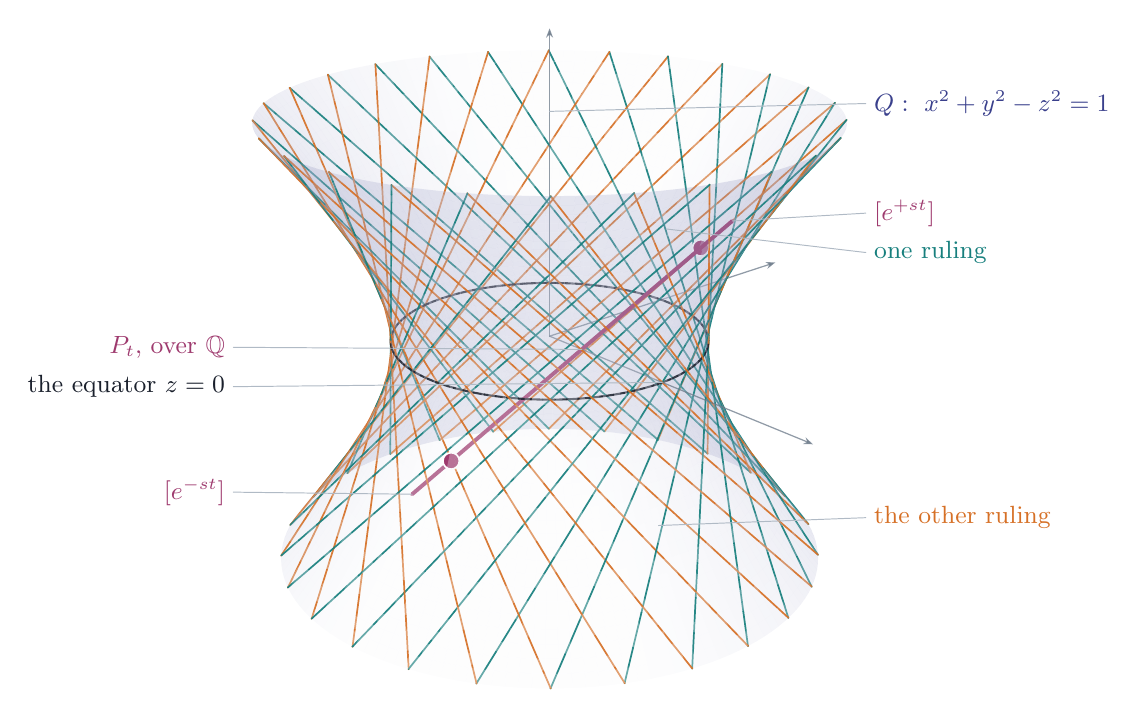
\begin{tikzpicture}[x=1cm,y=1cm,line join=round,line cap=round,
  font=\small,text=PInk]
  \path[draw=none,fill opacity=0.30,fill=PIndigo!42!white] (0.0396,-1.1770) -- (-0.0888,-1.1775) -- (-0.0866,-1.1158) -- (0.0386,-1.1154) -- cycle;
  \path[draw=none,fill opacity=0.30,fill=PIndigo!42!white] (0.1679,-1.1789) -- (0.0396,-1.1770) -- (0.0386,-1.1154) -- (0.1638,-1.1172) -- cycle;
  \path[draw=none,fill opacity=0.30,fill=PIndigo!42!white] (-0.0888,-1.1775) -- (-0.2170,-1.1803) -- (-0.2118,-1.1185) -- (-0.0866,-1.1158) -- cycle;
  \path[draw=none,fill opacity=0.30,fill=PIndigo!42!white] (0.2960,-1.1831) -- (0.1679,-1.1789) -- (0.1638,-1.1172) -- (0.2888,-1.1213) -- cycle;
  \draw[PAmber,line width=0.62pt,opacity=0.92] (0.0603,-1.1059) -- (-0.0110,-1.1769);
  \path[draw=none,fill opacity=0.30,fill=PIndigo!43!white] (-0.2170,-1.1803) -- (-0.3450,-1.1854) -- (-0.3366,-1.1235) -- (-0.2118,-1.1185) -- cycle;
  \path[draw=none,fill opacity=0.30,fill=PIndigo!41!white] (0.4237,-1.1897) -- (0.2960,-1.1831) -- (0.2888,-1.1213) -- (0.4134,-1.1277) -- cycle;
  \path[draw=none,fill opacity=0.30,fill=PIndigo!43!white] (-0.3450,-1.1854) -- (-0.4726,-1.1928) -- (-0.4611,-1.1307) -- (-0.3366,-1.1235) -- cycle;
  \path[draw=none,fill opacity=0.30,fill=PIndigo!41!white] (0.5510,-1.1986) -- (0.4237,-1.1897) -- (0.4134,-1.1277) -- (0.5375,-1.1363) -- cycle;
  \path[draw=none,fill opacity=0.30,fill=PIndigo!44!white] (-0.4726,-1.1928) -- (-0.5997,-1.2026) -- (-0.5850,-1.1402) -- (-0.4611,-1.1307) -- cycle;
  \path[draw=none,fill opacity=0.30,fill=PIndigo!41!white] (0.6776,-1.2098) -- (0.5510,-1.1986) -- (0.5375,-1.1363) -- (0.6610,-1.1471) -- cycle;
  \path[draw=none,fill opacity=0.30,fill=PIndigo!44!white] (-0.5997,-1.2026) -- (-0.7260,-1.2147) -- (-0.7082,-1.1519) -- (-0.5850,-1.1402) -- cycle;
  \draw[PTeal,line width=0.62pt,opacity=0.92] (-0.0086,-1.1769) -- (-0.0794,-1.1061) -- (-0.1510,-1.0344);
  \draw[PAmber,line width=0.62pt,opacity=0.92] (-0.6274,-1.1344) -- (-0.7174,-1.2138);
  \path[draw=none,fill opacity=0.30,fill=PIndigo!41!white] (0.8034,-1.2233) -- (0.6776,-1.2098) -- (0.6610,-1.1471) -- (0.7837,-1.1603) -- cycle;
  \draw[PAmber,line width=0.62pt,opacity=0.92] (0.7458,-1.1465) -- (0.6959,-1.2116);
  \path[draw=none,fill opacity=0.30,fill=PIndigo!45!white] (-0.7260,-1.2147) -- (-0.8514,-1.2291) -- (-0.8306,-1.1659) -- (-0.7082,-1.1519) -- cycle;
  \path[draw=none,fill opacity=0.30,fill=PIndigo!41!white] (0.9283,-1.2392) -- (0.8034,-1.2233) -- (0.7837,-1.1603) -- (0.9055,-1.1756) -- cycle;
  \path[draw=none,fill opacity=0.30,fill=PIndigo!42!white] (0.0386,-1.1154) -- (-0.0866,-1.1158) -- (-0.0845,-1.0528) -- (0.0376,-1.0524) -- cycle;
  \path[draw=none,fill opacity=0.30,fill=PIndigo!41!white] (0.1638,-1.1172) -- (0.0386,-1.1154) -- (0.0376,-1.0524) -- (0.1597,-1.0542) -- cycle;
  \path[draw=none,fill opacity=0.30,fill=PIndigo!42!white] (-0.0866,-1.1158) -- (-0.2118,-1.1185) -- (-0.2065,-1.0555) -- (-0.0845,-1.0528) -- cycle;
  \path[draw=none,fill opacity=0.30,fill=PIndigo!41!white] (0.2888,-1.1213) -- (0.1638,-1.1172) -- (0.1597,-1.0542) -- (0.2816,-1.0582) -- cycle;
  \path[draw=none,fill opacity=0.30,fill=PIndigo!45!white] (-0.8514,-1.2291) -- (-0.9759,-1.2459) -- (-0.9519,-1.1821) -- (-0.8306,-1.1659) -- cycle;
  \path[draw=none,fill opacity=0.30,fill=PIndigo!42!white] (-0.2118,-1.1185) -- (-0.3366,-1.1235) -- (-0.3283,-1.0603) -- (-0.2065,-1.0555) -- cycle;
  \draw[PTeal,line width=0.62pt,opacity=0.92] (0.6982,-1.2119) -- (0.6087,-1.1327) -- (0.5181,-1.0527);
  \path[draw=none,fill opacity=0.30,fill=PIndigo!41!white] (0.4134,-1.1277) -- (0.2888,-1.1213) -- (0.2816,-1.0582) -- (0.4031,-1.0643) -- cycle;
  \path[draw=none,fill opacity=0.30,fill=PIndigo!43!white] (-0.3366,-1.1235) -- (-0.4611,-1.1307) -- (-0.4496,-1.0673) -- (-0.3283,-1.0603) -- cycle;
  \path[draw=none,fill opacity=0.30,fill=PIndigo!42!white] (1.0520,-1.2573) -- (0.9283,-1.2392) -- (0.9055,-1.1756) -- (1.0261,-1.1932) -- cycle;
  \path[draw=none,fill opacity=0.30,fill=PIndigo!41!white] (0.5375,-1.1363) -- (0.4134,-1.1277) -- (0.4031,-1.0643) -- (0.5242,-1.0727) -- cycle;
  \path[draw=none,fill opacity=0.30,fill=PIndigo!43!white] (-0.4611,-1.1307) -- (-0.5850,-1.1402) -- (-0.5704,-1.0764) -- (-0.4496,-1.0673) -- cycle;
  \path[draw=none,fill opacity=0.30,fill=PIndigo!46!white] (-0.9759,-1.2459) -- (-1.0991,-1.2649) -- (-1.0721,-1.2005) -- (-0.9519,-1.1821) -- cycle;
  \draw[PTeal,line width=0.62pt,opacity=0.92] (-0.7151,-1.2136) -- (-0.7644,-1.1486) -- (-0.8145,-1.0826);
  \path[draw=none,fill opacity=0.30,fill=PIndigo!41!white] (0.6610,-1.1471) -- (0.5375,-1.1363) -- (0.5242,-1.0727) -- (0.6446,-1.0832) -- cycle;
  \path[draw=none,fill opacity=0.30,fill=PIndigo!44!white] (-0.5850,-1.1402) -- (-0.7082,-1.1519) -- (-0.6906,-1.0878) -- (-0.5704,-1.0764) -- cycle;
  \path[draw=none,fill opacity=0.30,fill=PIndigo!42!white] (1.1745,-1.2778) -- (1.0520,-1.2573) -- (1.0261,-1.1932) -- (1.1455,-1.2130) -- cycle;
  \path[draw=none,fill opacity=0.30,fill=PIndigo!41!white] (0.7837,-1.1603) -- (0.6610,-1.1471) -- (0.6446,-1.0832) -- (0.7642,-1.0959) -- cycle;
  \path[draw=none,fill opacity=0.30,fill=PIndigo!47!white] (-1.0991,-1.2649) -- (-1.2211,-1.2863) -- (-1.1910,-1.2212) -- (-1.0721,-1.2005) -- cycle;
  \path[draw=none,fill opacity=0.30,fill=PIndigo!44!white] (-0.7082,-1.1519) -- (-0.8306,-1.1659) -- (-0.8098,-1.1013) -- (-0.6906,-1.0878) -- cycle;
  \draw[PAmber,line width=0.62pt,opacity=0.92] (0.2057,-0.9611) -- (0.1325,-1.0340) -- (0.0603,-1.1059);
  \path[draw=none,fill opacity=0.30,fill=PIndigo!41!white] (0.9055,-1.1756) -- (0.7837,-1.1603) -- (0.7642,-1.0959) -- (0.8829,-1.1108) -- cycle;
  \path[draw=none,fill opacity=0.30,fill=PIndigo!41!white] (0.0376,-1.0524) -- (-0.0845,-1.0528) -- (-0.0823,-0.9885) -- (0.0367,-0.9881) -- cycle;
  \path[draw=none,fill opacity=0.30,fill=PIndigo!41!white] (0.1597,-1.0542) -- (0.0376,-1.0524) -- (0.0367,-0.9881) -- (0.1557,-0.9898) -- cycle;
  \path[draw=none,fill opacity=0.30,fill=PIndigo!42!white] (1.2955,-1.3005) -- (1.1745,-1.2778) -- (1.1455,-1.2130) -- (1.2635,-1.2351) -- cycle;
  \path[draw=none,fill opacity=0.30,fill=PIndigo!41!white] (-0.0845,-1.0528) -- (-0.2065,-1.0555) -- (-0.2013,-0.9911) -- (-0.0823,-0.9885) -- cycle;
  \path[draw=none,fill opacity=0.30,fill=PIndigo!41!white] (0.2816,-1.0582) -- (0.1597,-1.0542) -- (0.1557,-0.9898) -- (0.2745,-0.9937) -- cycle;
  \path[draw=none,fill opacity=0.30,fill=PIndigo!45!white] (-0.8306,-1.1659) -- (-0.9519,-1.1821) -- (-0.9281,-1.1171) -- (-0.8098,-1.1013) -- cycle;
  \path[draw=none,fill opacity=0.30,fill=PIndigo!42!white] (-0.2065,-1.0555) -- (-0.3283,-1.0603) -- (-0.3199,-0.9957) -- (-0.2013,-0.9911) -- cycle;
  \path[draw=none,fill opacity=0.30,fill=PIndigo!41!white] (0.4031,-1.0643) -- (0.2816,-1.0582) -- (0.2745,-0.9937) -- (0.3929,-0.9996) -- cycle;
  \path[draw=none,fill opacity=0.30,fill=PIndigo!47!white] (-1.2211,-1.2863) -- (-1.3415,-1.3099) -- (-1.3084,-1.2441) -- (-1.1910,-1.2212) -- cycle;
  \path[draw=none,fill opacity=0.30,fill=PIndigo!42!white] (-0.3283,-1.0603) -- (-0.4496,-1.0673) -- (-0.4382,-1.0025) -- (-0.3199,-0.9957) -- cycle;
  \draw[PAmber,line width=0.62pt,opacity=0.92] (-0.4443,-0.9729) -- (-0.5364,-1.0541) -- (-0.6274,-1.1344);
  \path[draw=none,fill opacity=0.30,fill=PIndigo!41!white] (1.0261,-1.1932) -- (0.9055,-1.1756) -- (0.8829,-1.1108) -- (1.0004,-1.1278) -- cycle;
  \path[draw=none,fill opacity=0.30,fill=PIndigo!40!white] (0.5242,-1.0727) -- (0.4031,-1.0643) -- (0.3929,-0.9996) -- (0.5109,-1.0077) -- cycle;
  \path[draw=none,fill opacity=0.30,fill=PIndigo!43!white] (-0.4496,-1.0673) -- (-0.5704,-1.0764) -- (-0.5560,-1.0114) -- (-0.4382,-1.0025) -- cycle;
  \path[draw=none,fill opacity=0.30,fill=PIndigo!46!white] (-0.9519,-1.1821) -- (-1.0721,-1.2005) -- (-1.0452,-1.1349) -- (-0.9281,-1.1171) -- cycle;
  \path[draw=none,fill opacity=0.30,fill=PIndigo!42!white] (1.4149,-1.3256) -- (1.2955,-1.3005) -- (1.2635,-1.2351) -- (1.3799,-1.2593) -- cycle;
  \path[draw=none,fill opacity=0.30,fill=PIndigo!40!white] (0.6446,-1.0832) -- (0.5242,-1.0727) -- (0.5109,-1.0077) -- (0.6282,-1.0179) -- cycle;
  \path[draw=none,fill opacity=0.30,fill=PIndigo!43!white] (-0.5704,-1.0764) -- (-0.6906,-1.0878) -- (-0.6730,-1.0224) -- (-0.5560,-1.0114) -- cycle;
  \draw[PAmber,line width=0.62pt,opacity=0.92] (-1.2919,-1.2315) -- (-1.3976,-1.3218);
  \path[draw=none,fill opacity=0.30,fill=PIndigo!41!white] (1.1455,-1.2130) -- (1.0261,-1.1932) -- (1.0004,-1.1278) -- (1.1168,-1.1470) -- cycle;
  \path[draw=none,fill opacity=0.30,fill=PIndigo!48!white] (-1.3415,-1.3099) -- (-1.4603,-1.3358) -- (-1.4241,-1.2692) -- (-1.3084,-1.2441) -- cycle;
  \path[draw=none,fill opacity=0.30,fill=PIndigo!40!white] (0.7642,-1.0959) -- (0.6446,-1.0832) -- (0.6282,-1.0179) -- (0.7448,-1.0302) -- cycle;
  \draw[PAmber,line width=0.62pt,opacity=0.92] (0.8479,-1.0133) -- (0.7965,-1.0804) -- (0.7458,-1.1465);
  \draw[PAmber,line width=0.62pt,opacity=0.92] (1.4035,-1.2554) -- (1.3773,-1.3174);
  \path[draw=none,fill opacity=0.30,fill=PIndigo!46!white] (-1.0721,-1.2005) -- (-1.1910,-1.2212) -- (-1.1611,-1.1549) -- (-1.0452,-1.1349) -- cycle;
  \path[draw=none,fill opacity=0.30,fill=PIndigo!44!white] (-0.6906,-1.0878) -- (-0.8098,-1.1013) -- (-0.7893,-1.0355) -- (-0.6730,-1.0224) -- cycle;
  \draw[PTeal,line width=0.62pt,opacity=0.92] (1.3795,-1.3179) -- (1.2741,-1.2280) -- (1.1677,-1.1372);
  \path[draw=none,fill opacity=0.30,fill=PIndigo!43!white] (1.5326,-1.3529) -- (1.4149,-1.3256) -- (1.3799,-1.2593) -- (1.4946,-1.2857) -- cycle;
  \path[draw=none,fill opacity=0.30,fill=PIndigo!41!white] (0.8829,-1.1108) -- (0.7642,-1.0959) -- (0.7448,-1.0302) -- (0.8604,-1.0446) -- cycle;
  \path[draw=none,fill opacity=0.30,fill=PIndigo!42!white] (1.2635,-1.2351) -- (1.1455,-1.2130) -- (1.1168,-1.1470) -- (1.2317,-1.1683) -- cycle;
  \path[draw=none,fill opacity=0.30,fill=PIndigo!41!white] (0.0367,-0.9881) -- (-0.0823,-0.9885) -- (-0.0802,-0.9228) -- (0.0357,-0.9224) -- cycle;
  \path[draw=none,fill opacity=0.30,fill=PIndigo!40!white] (0.1557,-0.9898) -- (0.0367,-0.9881) -- (0.0357,-0.9224) -- (0.1517,-0.9241) -- cycle;
  \path[draw=none,fill opacity=0.30,fill=PIndigo!41!white] (-0.0823,-0.9885) -- (-0.2013,-0.9911) -- (-0.1961,-0.9252) -- (-0.0802,-0.9228) -- cycle;
  \draw[PTeal,line width=0.62pt,opacity=0.92] (-0.1510,-1.0344) -- (-0.2237,-0.9617) -- (-0.2973,-0.8880);
  \path[draw=none,fill opacity=0.30,fill=PIndigo!44!white] (-0.8098,-1.1013) -- (-0.9281,-1.1171) -- (-0.9045,-1.0507) -- (-0.7893,-1.0355) -- cycle;
  \path[draw=none,fill opacity=0.30,fill=PIndigo!40!white] (0.2745,-0.9937) -- (0.1557,-0.9898) -- (0.1517,-0.9241) -- (0.2674,-0.9278) -- cycle;
  \path[draw=none,fill opacity=0.30,fill=PIndigo!41!white] (-0.2013,-0.9911) -- (-0.3199,-0.9957) -- (-0.3117,-0.9297) -- (-0.1961,-0.9252) -- cycle;
  \path[draw=none,fill opacity=0.30,fill=PIndigo!49!white] (-1.4603,-1.3358) -- (-1.5773,-1.3639) -- (-1.5381,-1.2964) -- (-1.4241,-1.2692) -- cycle;
  \path[draw=none,fill opacity=0.30,fill=PIndigo!47!white] (-1.1910,-1.2212) -- (-1.3084,-1.2441) -- (-1.2754,-1.1771) -- (-1.1611,-1.1549) -- cycle;
  \path[draw=none,fill opacity=0.30,fill=PIndigo!40!white] (0.3929,-0.9996) -- (0.2745,-0.9937) -- (0.2674,-0.9278) -- (0.3828,-0.9335) -- cycle;
  \path[draw=none,fill opacity=0.30,fill=PIndigo!42!white] (-0.3199,-0.9957) -- (-0.4382,-1.0025) -- (-0.4270,-0.9363) -- (-0.3117,-0.9297) -- cycle;
  \draw[PTeal,line width=0.62pt,opacity=0.92] (0.5181,-1.0527) -- (0.4265,-0.9717) -- (0.3338,-0.8898);
  \path[draw=none,fill opacity=0.30,fill=PIndigo!41!white] (1.0004,-1.1278) -- (0.8829,-1.1108) -- (0.8604,-1.0446) -- (0.9750,-1.0611) -- cycle;
  \path[draw=none,fill opacity=0.30,fill=PIndigo!40!white] (0.5109,-1.0077) -- (0.3929,-0.9996) -- (0.3828,-0.9335) -- (0.4977,-0.9414) -- cycle;
  \path[draw=none,fill opacity=0.30,fill=PIndigo!42!white] (-0.4382,-1.0025) -- (-0.5560,-1.0114) -- (-0.5417,-0.9449) -- (-0.4270,-0.9363) -- cycle;
  \path[draw=none,fill opacity=0.30,fill=PIndigo!45!white] (-0.9281,-1.1171) -- (-1.0452,-1.1349) -- (-1.0186,-1.0680) -- (-0.9045,-1.0507) -- cycle;
  \path[draw=none,fill opacity=0.30,fill=PIndigo!42!white] (1.3799,-1.2593) -- (1.2635,-1.2351) -- (1.2317,-1.1683) -- (1.3451,-1.1918) -- cycle;
  \path[draw=none,fill opacity=0.30,fill=PIndigo!43!white] (1.6484,-1.3824) -- (1.5326,-1.3529) -- (1.4946,-1.2857) -- (1.6074,-1.3143) -- cycle;
  \path[draw=none,fill opacity=0.30,fill=PIndigo!40!white] (0.6282,-1.0179) -- (0.5109,-1.0077) -- (0.4977,-0.9414) -- (0.6120,-0.9512) -- cycle;
  \draw[PTeal,line width=0.62pt,opacity=0.92] (-1.3954,-1.3213) -- (-1.4210,-1.2594) -- (-1.4470,-1.1965);
  \path[draw=none,fill opacity=0.30,fill=PIndigo!43!white] (-0.5560,-1.0114) -- (-0.6730,-1.0224) -- (-0.6557,-0.9555) -- (-0.5417,-0.9449) -- cycle;
  \path[draw=none,fill opacity=0.30,fill=PIndigo!41!white] (1.1168,-1.1470) -- (1.0004,-1.1278) -- (0.9750,-1.0611) -- (1.0883,-1.0797) -- cycle;
  \path[draw=none,fill opacity=0.30,fill=PIndigo!48!white] (-1.3084,-1.2441) -- (-1.4241,-1.2692) -- (-1.3882,-1.2014) -- (-1.2754,-1.1771) -- cycle;
  \path[draw=none,fill opacity=0.30,fill=PIndigo!50!white] (-1.5773,-1.3639) -- (-1.6923,-1.3943) -- (-1.6501,-1.3259) -- (-1.5381,-1.2964) -- cycle;
  \path[draw=none,fill opacity=0.30,fill=PIndigo!40!white] (0.7448,-1.0302) -- (0.6282,-1.0179) -- (0.6120,-0.9512) -- (0.7256,-0.9631) -- cycle;
  \path[draw=none,fill opacity=0.30,fill=PIndigo!46!white] (-1.0452,-1.1349) -- (-1.1611,-1.1549) -- (-1.1314,-1.0873) -- (-1.0186,-1.0680) -- cycle;
  \path[draw=none,fill opacity=0.30,fill=PIndigo!43!white] (-0.6730,-1.0224) -- (-0.7893,-1.0355) -- (-0.7689,-0.9682) -- (-0.6557,-0.9555) -- cycle;
  \draw[PAmber,line width=0.62pt,opacity=0.92] (-1.0773,-1.0485) -- (-1.1851,-1.1404) -- (-1.2919,-1.2315);
  \path[draw=none,fill opacity=0.30,fill=PIndigo!42!white] (1.4946,-1.2857) -- (1.3799,-1.2593) -- (1.3451,-1.1918) -- (1.4568,-1.2174) -- cycle;
  \path[draw=none,fill opacity=0.30,fill=PIndigo!40!white] (0.8604,-1.0446) -- (0.7448,-1.0302) -- (0.7256,-0.9631) -- (0.8382,-0.9770) -- cycle;
  \path[draw=none,fill opacity=0.30,fill=PIndigo!41!white] (1.2317,-1.1683) -- (1.1168,-1.1470) -- (1.0883,-1.0797) -- (1.2002,-1.1003) -- cycle;
  \path[draw=none,fill opacity=0.30,fill=PIndigo!40!white] (0.0357,-0.9224) -- (-0.0802,-0.9228) -- (-0.0781,-0.8556) -- (0.0348,-0.8552) -- cycle;
  \path[draw=none,fill opacity=0.30,fill=PIndigo!44!white] (1.7621,-1.4141) -- (1.6484,-1.3824) -- (1.6074,-1.3143) -- (1.7181,-1.3451) -- cycle;
  \path[draw=none,fill opacity=0.30,fill=PIndigo!40!white] (0.1517,-0.9241) -- (0.0357,-0.9224) -- (0.0348,-0.8552) -- (0.1477,-0.8568) -- cycle;
  \path[draw=none,fill opacity=0.30,fill=PIndigo!40!white] (-0.0802,-0.9228) -- (-0.1961,-0.9252) -- (-0.1910,-0.8579) -- (-0.0781,-0.8556) -- cycle;
  \path[draw=none,fill opacity=0.30,fill=PIndigo!44!white] (-0.7893,-1.0355) -- (-0.9045,-1.0507) -- (-0.8811,-0.9829) -- (-0.7689,-0.9682) -- cycle;
  \path[draw=none,fill opacity=0.30,fill=PIndigo!40!white] (0.2674,-0.9278) -- (0.1517,-0.9241) -- (0.1477,-0.8568) -- (0.2605,-0.8604) -- cycle;
  \draw[PTeal,line width=0.62pt,opacity=0.92] (-0.8145,-1.0826) -- (-0.8653,-1.0156) -- (-0.9168,-0.9477);
  \path[draw=none,fill opacity=0.30,fill=PIndigo!49!white] (-1.4241,-1.2692) -- (-1.5381,-1.2964) -- (-1.4992,-1.2277) -- (-1.3882,-1.2014) -- cycle;
  \path[draw=none,fill opacity=0.30,fill=PIndigo!41!white] (-0.1961,-0.9252) -- (-0.3117,-0.9297) -- (-0.3036,-0.8623) -- (-0.1910,-0.8579) -- cycle;
  \path[draw=none,fill opacity=0.30,fill=PIndigo!47!white] (-1.1611,-1.1549) -- (-1.2754,-1.1771) -- (-1.2428,-1.1088) -- (-1.1314,-1.0873) -- cycle;
  \path[draw=none,fill opacity=0.30,fill=PIndigo!40!white] (0.3828,-0.9335) -- (0.2674,-0.9278) -- (0.2605,-0.8604) -- (0.3729,-0.8659) -- cycle;
  \path[draw=none,fill opacity=0.30,fill=PIndigo!41!white] (-0.3117,-0.9297) -- (-0.4270,-0.9363) -- (-0.4159,-0.8686) -- (-0.3036,-0.8623) -- cycle;
  \path[draw=none,fill opacity=0.30,fill=PIndigo!40!white] (0.9750,-1.0611) -- (0.8604,-1.0446) -- (0.8382,-0.9770) -- (0.9498,-0.9930) -- cycle;
  \draw[PAmber,line width=0.62pt,opacity=0.92] (0.3551,-0.8123) -- (0.2799,-0.8872) -- (0.2057,-0.9611);
  \path[draw=none,fill opacity=0.30,fill=PIndigo!50!white] (-1.6923,-1.3943) -- (-1.8051,-1.4269) -- (-1.7600,-1.3574) -- (-1.6501,-1.3259) -- cycle;
  \path[draw=none,fill opacity=0.30,fill=PIndigo!39!white] (0.4977,-0.9414) -- (0.3828,-0.9335) -- (0.3729,-0.8659) -- (0.4848,-0.8735) -- cycle;
  \draw[PAmber,line width=0.62pt,opacity=0.92] (-0.2568,-0.8075) -- (-0.3511,-0.8907) -- (-0.4443,-0.9729);
  \path[draw=none,fill opacity=0.30,fill=PIndigo!45!white] (-0.9045,-1.0507) -- (-1.0186,-1.0680) -- (-0.9922,-0.9996) -- (-0.8811,-0.9829) -- cycle;
  \path[draw=none,fill opacity=0.30,fill=PIndigo!42!white] (-0.4270,-0.9363) -- (-0.5417,-0.9449) -- (-0.5276,-0.8769) -- (-0.4159,-0.8686) -- cycle;
  \path[draw=none,fill opacity=0.30,fill=PIndigo!41!white] (1.3451,-1.1918) -- (1.2317,-1.1683) -- (1.2002,-1.1003) -- (1.3107,-1.1230) -- cycle;
  \path[draw=none,fill opacity=0.30,fill=PIndigo!43!white] (1.6074,-1.3143) -- (1.4946,-1.2857) -- (1.4568,-1.2174) -- (1.5667,-1.2450) -- cycle;
  \path[draw=none,fill opacity=0.30,fill=PIndigo!39!white] (0.6120,-0.9512) -- (0.4977,-0.9414) -- (0.4848,-0.8735) -- (0.5961,-0.8830) -- cycle;
  \path[draw=none,fill opacity=0.30,fill=PIndigo!42!white] (-0.5417,-0.9449) -- (-0.6557,-0.9555) -- (-0.6386,-0.8872) -- (-0.5276,-0.8769) -- cycle;
  \path[draw=none,fill opacity=0.30,fill=PIndigo!47!white] (-1.2754,-1.1771) -- (-1.3882,-1.2014) -- (-1.3526,-1.1323) -- (-1.2428,-1.1088) -- cycle;
  \path[draw=none,fill opacity=0.30,fill=PIndigo!40!white] (1.0883,-1.0797) -- (0.9750,-1.0611) -- (0.9498,-0.9930) -- (1.0601,-1.0109) -- cycle;
  \path[draw=none,fill opacity=0.30,fill=PIndigo!50!white] (-1.5381,-1.2964) -- (-1.6501,-1.3259) -- (-1.6083,-1.2562) -- (-1.4992,-1.2277) -- cycle;
  \path[draw=none,fill opacity=0.30,fill=PIndigo!44!white] (1.8736,-1.4481) -- (1.7621,-1.4141) -- (1.7181,-1.3451) -- (1.8266,-1.3780) -- cycle;
  \draw[PTeal,line width=0.62pt,opacity=0.92] (1.1677,-1.1372) -- (1.0603,-1.0455) -- (0.9519,-0.9530);
  \path[draw=none,fill opacity=0.30,fill=PIndigo!39!white] (0.7256,-0.9631) -- (0.6120,-0.9512) -- (0.5961,-0.8830) -- (0.7066,-0.8945) -- cycle;
  \path[draw=none,fill opacity=0.30,fill=PIndigo!45!white] (-1.0186,-1.0680) -- (-1.1314,-1.0873) -- (-1.1021,-1.0184) -- (-0.9922,-0.9996) -- cycle;
  \path[draw=none,fill opacity=0.30,fill=PIndigo!43!white] (-0.6557,-0.9555) -- (-0.7689,-0.9682) -- (-0.7488,-0.8995) -- (-0.6386,-0.8872) -- cycle;
  \draw[PAmber,line width=0.62pt,opacity=0.92] (1.4572,-1.1286) -- (1.4302,-1.1925) -- (1.4035,-1.2554);
  \path[draw=none,fill opacity=0.30,fill=PIndigo!42!white] (1.4568,-1.2174) -- (1.3451,-1.1918) -- (1.3107,-1.1230) -- (1.4194,-1.1477) -- cycle;
  \path[draw=none,fill opacity=0.30,fill=PIndigo!50!white] (-1.8051,-1.4269) -- (-1.9157,-1.4617) -- (-1.8676,-1.3911) -- (-1.7600,-1.3574) -- cycle;
  \path[draw=none,fill opacity=0.30,fill=PIndigo!40!white] (0.8382,-0.9770) -- (0.7256,-0.9631) -- (0.7066,-0.8945) -- (0.8163,-0.9080) -- cycle;
  \path[draw=none,fill opacity=0.30,fill=PIndigo!41!white] (1.2002,-1.1003) -- (1.0883,-1.0797) -- (1.0601,-1.0109) -- (1.1691,-1.0309) -- cycle;
  \path[draw=none,fill opacity=0.30,fill=PIndigo!43!white] (1.7181,-1.3451) -- (1.6074,-1.3143) -- (1.5667,-1.2450) -- (1.6744,-1.2748) -- cycle;
  \path[draw=none,fill opacity=0.30,fill=PIndigo!40!white] (0.0348,-0.8552) -- (-0.0781,-0.8556) -- (-0.0761,-0.7867) -- (0.0339,-0.7864) -- cycle;
  \path[draw=none,fill opacity=0.30,fill=PIndigo!39!white] (0.1477,-0.8568) -- (0.0348,-0.8552) -- (0.0339,-0.7864) -- (0.1438,-0.7879) -- cycle;
  \path[draw=none,fill opacity=0.30,fill=PIndigo!44!white] (-0.7689,-0.9682) -- (-0.8811,-0.9829) -- (-0.8581,-0.9137) -- (-0.7488,-0.8995) -- cycle;
  \path[draw=none,fill opacity=0.30,fill=PIndigo!48!white] (-1.3882,-1.2014) -- (-1.4992,-1.2277) -- (-1.4606,-1.1578) -- (-1.3526,-1.1323) -- cycle;
  \path[draw=none,fill opacity=0.30,fill=PIndigo!40!white] (-0.0781,-0.8556) -- (-0.1910,-0.8579) -- (-0.1860,-0.7890) -- (-0.0761,-0.7867) -- cycle;
  \path[draw=none,fill opacity=0.30,fill=PIndigo!39!white] (0.2605,-0.8604) -- (0.1477,-0.8568) -- (0.1438,-0.7879) -- (0.2536,-0.7914) -- cycle;
  \path[draw=none,fill opacity=0.30,fill=PIndigo!46!white] (-1.1314,-1.0873) -- (-1.2428,-1.1088) -- (-1.2105,-1.0391) -- (-1.1021,-1.0184) -- cycle;
  \path[draw=none,fill opacity=0.30,fill=PIndigo!40!white] (-0.1910,-0.8579) -- (-0.3036,-0.8623) -- (-0.2956,-0.7932) -- (-0.1860,-0.7890) -- cycle;
  \path[draw=none,fill opacity=0.30,fill=PIndigo!39!white] (0.3729,-0.8659) -- (0.2605,-0.8604) -- (0.2536,-0.7914) -- (0.3630,-0.7968) -- cycle;
  \path[draw=none,fill opacity=0.30,fill=PIndigo!50!white] (-1.6501,-1.3259) -- (-1.7600,-1.3574) -- (-1.7152,-1.2868) -- (-1.6083,-1.2562) -- cycle;
  \path[draw=none,fill opacity=0.30,fill=PIndigo!41!white] (-0.3036,-0.8623) -- (-0.4159,-0.8686) -- (-0.4049,-0.7993) -- (-0.2956,-0.7932) -- cycle;
  \path[draw=none,fill opacity=0.30,fill=PIndigo!40!white] (0.9498,-0.9930) -- (0.8382,-0.9770) -- (0.8163,-0.9080) -- (0.9249,-0.9234) -- cycle;
  \path[draw=none,fill opacity=0.30,fill=PIndigo!45!white] (1.9826,-1.4843) -- (1.8736,-1.4481) -- (1.8266,-1.3780) -- (1.9328,-1.4130) -- cycle;
  \path[draw=none,fill opacity=0.30,fill=PIndigo!39!white] (0.4848,-0.8735) -- (0.3729,-0.8659) -- (0.3630,-0.7968) -- (0.4720,-0.8041) -- cycle;
  \path[draw=none,fill opacity=0.30,fill=PIndigo!44!white] (-0.8811,-0.9829) -- (-0.9922,-0.9996) -- (-0.9662,-0.9298) -- (-0.8581,-0.9137) -- cycle;
  \path[draw=none,fill opacity=0.30,fill=PIndigo!42!white] (1.5667,-1.2450) -- (1.4568,-1.2174) -- (1.4194,-1.1477) -- (1.5263,-1.1745) -- cycle;
  \path[draw=none,fill opacity=0.30,fill=PIndigo!41!white] (1.3107,-1.1230) -- (1.2002,-1.1003) -- (1.1691,-1.0309) -- (1.2766,-1.0529) -- cycle;
  \path[draw=none,fill opacity=0.30,fill=PIndigo!41!white] (-0.4159,-0.8686) -- (-0.5276,-0.8769) -- (-0.5137,-0.8074) -- (-0.4049,-0.7993) -- cycle;
  \draw[PTeal,line width=0.62pt,opacity=0.92] (0.3338,-0.8898) -- (0.2400,-0.8068) -- (0.1450,-0.7230);
  \draw[PAmber,line width=0.62pt,opacity=0.92] (0.9530,-0.8762) -- (0.9001,-0.9452) -- (0.8479,-1.0133);
  \path[draw=none,fill opacity=0.30,fill=PIndigo!39!white] (0.5961,-0.8830) -- (0.4848,-0.8735) -- (0.4720,-0.8041) -- (0.5804,-0.8133) -- cycle;
  \draw[PTeal,line width=0.62pt,opacity=0.92] (-0.2973,-0.8880) -- (-0.3719,-0.8133) -- (-0.4475,-0.7375);
  \path[draw=none,fill opacity=0.30,fill=PIndigo!47!white] (-1.2428,-1.1088) -- (-1.3526,-1.1323) -- (-1.3173,-1.0618) -- (-1.2105,-1.0391) -- cycle;
  \path[draw=none,fill opacity=0.30,fill=PIndigo!50!white] (-1.9157,-1.4617) -- (-2.0238,-1.4987) -- (-1.9728,-1.4269) -- (-1.8676,-1.3911) -- cycle;
  \path[draw=none,fill opacity=0.30,fill=PIndigo!42!white] (-0.5276,-0.8769) -- (-0.6386,-0.8872) -- (-0.6218,-0.8173) -- (-0.5137,-0.8074) -- cycle;
  \path[draw=none,fill opacity=0.30,fill=PIndigo!40!white] (1.0601,-1.0109) -- (0.9498,-0.9930) -- (0.9249,-0.9234) -- (1.0323,-0.9408) -- cycle;
  \path[draw=none,fill opacity=0.30,fill=PIndigo!44!white] (1.8266,-1.3780) -- (1.7181,-1.3451) -- (1.6744,-1.2748) -- (1.7801,-1.3066) -- cycle;
  \path[draw=none,fill opacity=0.30,fill=PIndigo!49!white] (-1.4992,-1.2277) -- (-1.6083,-1.2562) -- (-1.5668,-1.1853) -- (-1.4606,-1.1578) -- cycle;
  \draw[PAmber,line width=0.62pt,opacity=0.92] (-0.8586,-0.8619) -- (-0.9685,-0.9556) -- (-1.0773,-1.0485);
  \path[draw=none,fill opacity=0.30,fill=PIndigo!39!white] (0.7066,-0.8945) -- (0.5961,-0.8830) -- (0.5804,-0.8133) -- (0.6880,-0.8244) -- cycle;
  \path[draw=none,fill opacity=0.30,fill=PIndigo!45!white] (-0.9922,-0.9996) -- (-1.1021,-1.0184) -- (-1.0731,-0.9479) -- (-0.9662,-0.9298) -- cycle;
  \draw[PAmber,line width=0.62pt,opacity=0.92] (-1.9067,-1.3956) -- (-2.0247,-1.4991);
  \path[draw=none,fill opacity=0.30,fill=PIndigo!42!white] (-0.6386,-0.8872) -- (-0.7488,-0.8995) -- (-0.7290,-0.8292) -- (-0.6218,-0.8173) -- cycle;
  \path[draw=none,fill opacity=0.30,fill=PIndigo!50!white] (-1.7600,-1.3574) -- (-1.8676,-1.3911) -- (-1.8199,-1.3194) -- (-1.7152,-1.2868) -- cycle;
  \path[draw=none,fill opacity=0.30,fill=PIndigo!41!white] (1.4194,-1.1477) -- (1.3107,-1.1230) -- (1.2766,-1.0529) -- (1.3824,-1.0768) -- cycle;
  \path[draw=none,fill opacity=0.30,fill=PIndigo!43!white] (1.6744,-1.2748) -- (1.5667,-1.2450) -- (1.5263,-1.1745) -- (1.6312,-1.2033) -- cycle;
  \path[draw=none,fill opacity=0.30,fill=PIndigo!40!white] (1.1691,-1.0309) -- (1.0601,-1.0109) -- (1.0323,-0.9408) -- (1.1383,-0.9601) -- cycle;
  \path[draw=none,fill opacity=0.30,fill=PIndigo!39!white] (0.8163,-0.9080) -- (0.7066,-0.8945) -- (0.6880,-0.8244) -- (0.7947,-0.8374) -- cycle;
  \path[draw=none,fill opacity=0.30,fill=PIndigo!45!white] (2.0891,-1.5226) -- (1.9826,-1.4843) -- (1.9328,-1.4130) -- (2.0364,-1.4500) -- cycle;
  \draw[PTeal,line width=0.62pt,opacity=0.92] (2.0084,-1.4933) -- (1.8906,-1.3902) -- (1.7721,-1.2864);
  \path[draw=none,fill opacity=0.30,fill=PIndigo!48!white] (-1.3526,-1.1323) -- (-1.4606,-1.1578) -- (-1.4225,-1.0865) -- (-1.3173,-1.0618) -- cycle;
  \path[draw=none,fill opacity=0.30,fill=PIndigo!39!white] (0.0339,-0.7864) -- (-0.0761,-0.7867) -- (-0.0741,-0.7162) -- (0.0330,-0.7159) -- cycle;
  \path[draw=none,fill opacity=0.30,fill=PIndigo!43!white] (-0.7488,-0.8995) -- (-0.8581,-0.9137) -- (-0.8354,-0.8429) -- (-0.7290,-0.8292) -- cycle;
  \draw[PAmber,line width=0.62pt,opacity=0.92] (2.0069,-1.4309) -- (2.0064,-1.4926);
  \path[draw=none,fill opacity=0.30,fill=PIndigo!39!white] (0.1438,-0.7879) -- (0.0339,-0.7864) -- (0.0330,-0.7159) -- (0.1400,-0.7174) -- cycle;
  \path[draw=none,fill opacity=0.30,fill=PIndigo!39!white] (-0.0761,-0.7867) -- (-0.1860,-0.7890) -- (-0.1811,-0.7184) -- (-0.0741,-0.7162) -- cycle;
  \path[draw=none,fill opacity=0.30,fill=PIndigo!46!white] (-1.1021,-1.0184) -- (-1.2105,-1.0391) -- (-1.1786,-0.9680) -- (-1.0731,-0.9479) -- cycle;
  \path[draw=none,fill opacity=0.30,fill=PIndigo!38!white] (0.2536,-0.7914) -- (0.1438,-0.7879) -- (0.1400,-0.7174) -- (0.2469,-0.7207) -- cycle;
  \path[draw=none,fill opacity=0.30,fill=PIndigo!40!white] (-0.1860,-0.7890) -- (-0.2956,-0.7932) -- (-0.2878,-0.7225) -- (-0.1811,-0.7184) -- cycle;
  \path[draw=none,fill opacity=0.30,fill=PIndigo!50!white] (-1.6083,-1.2562) -- (-1.7152,-1.2868) -- (-1.6708,-1.2149) -- (-1.5668,-1.1853) -- cycle;
  \path[draw=none,fill opacity=0.30,fill=PIndigo!38!white] (0.3630,-0.7968) -- (0.2536,-0.7914) -- (0.2469,-0.7207) -- (0.3534,-0.7259) -- cycle;
  \path[draw=none,fill opacity=0.30,fill=PIndigo!44!white] (1.9328,-1.4130) -- (1.8266,-1.3780) -- (1.7801,-1.3066) -- (1.8833,-1.3405) -- cycle;
  \path[draw=none,fill opacity=0.30,fill=PIndigo!39!white] (0.9249,-0.9234) -- (0.8163,-0.9080) -- (0.7947,-0.8374) -- (0.9004,-0.8523) -- cycle;
  \path[draw=none,fill opacity=0.30,fill=PIndigo!40!white] (-0.2956,-0.7932) -- (-0.4049,-0.7993) -- (-0.3942,-0.7284) -- (-0.2878,-0.7225) -- cycle;
  \path[draw=none,fill opacity=0.30,fill=PIndigo!50!white] (-2.0238,-1.4987) -- (-2.1292,-1.5378) -- (-2.0754,-1.4648) -- (-1.9728,-1.4269) -- cycle;
  \path[draw=none,fill opacity=0.30,fill=PIndigo!38!white] (0.4720,-0.8041) -- (0.3630,-0.7968) -- (0.3534,-0.7259) -- (0.4595,-0.7330) -- cycle;
  \path[draw=none,fill opacity=0.30,fill=PIndigo!42!white] (1.5263,-1.1745) -- (1.4194,-1.1477) -- (1.3824,-1.0768) -- (1.4863,-1.1026) -- cycle;
  \path[draw=none,fill opacity=0.30,fill=PIndigo!40!white] (1.2766,-1.0529) -- (1.1691,-1.0309) -- (1.1383,-0.9601) -- (1.2429,-0.9813) -- cycle;
  \path[draw=none,fill opacity=0.30,fill=PIndigo!44!white] (-0.8581,-0.9137) -- (-0.9662,-0.9298) -- (-0.9406,-0.8585) -- (-0.8354,-0.8429) -- cycle;
  \draw[PTeal,line width=0.62pt,opacity=0.92] (-1.4470,-1.1965) -- (-1.4733,-1.1326) -- (-1.5001,-1.0678);
  \path[draw=none,fill opacity=0.30,fill=PIndigo!41!white] (-0.4049,-0.7993) -- (-0.5137,-0.8074) -- (-0.5000,-0.7362) -- (-0.3942,-0.7284) -- cycle;
  \draw[PTeal,line width=0.62pt,opacity=0.92] (0.9519,-0.9530) -- (0.8424,-0.8596) -- (0.7318,-0.7653);
  \path[draw=none,fill opacity=0.30,fill=PIndigo!50!white] (-1.8676,-1.3911) -- (-1.9728,-1.4269) -- (-1.9223,-1.3540) -- (-1.8199,-1.3194) -- cycle;
  \path[draw=none,fill opacity=0.30,fill=PIndigo!38!white] (0.5804,-0.8133) -- (0.4720,-0.8041) -- (0.4595,-0.7330) -- (0.5650,-0.7419) -- cycle;
  \path[draw=none,fill opacity=0.30,fill=PIndigo!43!white] (1.7801,-1.3066) -- (1.6744,-1.2748) -- (1.6312,-1.2033) -- (1.7339,-1.2340) -- cycle;
  \draw[PAmber,line width=0.62pt,opacity=0.92] (-0.0649,-0.6382) -- (-0.1614,-0.7234) -- (-0.2568,-0.8075);
  \path[draw=none,fill opacity=0.30,fill=PIndigo!47!white] (-1.2105,-1.0391) -- (-1.3173,-1.0618) -- (-1.2826,-0.9899) -- (-1.1786,-0.9680) -- cycle;
  \path[draw=none,fill opacity=0.30,fill=PIndigo!49!white] (-1.4606,-1.1578) -- (-1.5668,-1.1853) -- (-1.5257,-1.1131) -- (-1.4225,-1.0865) -- cycle;
  \path[draw=none,fill opacity=0.30,fill=PIndigo!39!white] (1.0323,-0.9408) -- (0.9249,-0.9234) -- (0.9004,-0.8523) -- (1.0049,-0.8691) -- cycle;
  \path[draw=none,fill opacity=0.30,fill=PIndigo!41!white] (-0.5137,-0.8074) -- (-0.6218,-0.8173) -- (-0.6053,-0.7458) -- (-0.5000,-0.7362) -- cycle;
  \path[draw=none,fill opacity=0.30,fill=PIndigo!44!white] (-0.9662,-0.9298) -- (-1.0731,-0.9479) -- (-1.0447,-0.8760) -- (-0.9406,-0.8585) -- cycle;
  \path[draw=none,fill opacity=0.30,fill=PIndigo!38!white] (0.6880,-0.8244) -- (0.5804,-0.8133) -- (0.5650,-0.7419) -- (0.6697,-0.7526) -- cycle;
  \path[draw=none,fill opacity=0.30,fill=PIndigo!46!white] (2.1928,-1.5630) -- (2.0891,-1.5226) -- (2.0364,-1.4500) -- (2.1372,-1.4892) -- cycle;
  \path[draw=none,fill opacity=0.30,fill=PIndigo!50!white] (-1.7152,-1.2868) -- (-1.8199,-1.3194) -- (-1.7727,-1.2464) -- (-1.6708,-1.2149) -- cycle;
  \draw[PAmber,line width=0.62pt,opacity=0.92] (-1.6681,-1.1865) -- (-1.7878,-1.2914) -- (-1.9067,-1.3956);
  \draw[PAmber,line width=0.62pt,opacity=0.92] (0.5086,-0.6594) -- (0.4313,-0.7364) -- (0.3551,-0.8123);
  \path[draw=none,fill opacity=0.30,fill=PIndigo!42!white] (-0.6218,-0.8173) -- (-0.7290,-0.8292) -- (-0.7097,-0.7572) -- (-0.6053,-0.7458) -- cycle;
  \path[draw=none,fill opacity=0.30,fill=PIndigo!41!white] (1.3824,-1.0768) -- (1.2766,-1.0529) -- (1.2429,-0.9813) -- (1.3458,-1.0044) -- cycle;
  \draw[PTeal,line width=0.62pt,opacity=0.92] (-0.9168,-0.9477) -- (-0.9691,-0.8787) -- (-1.0222,-0.8088);
  \path[draw=none,fill opacity=0.30,fill=PIndigo!42!white] (1.6312,-1.2033) -- (1.5263,-1.1745) -- (1.4863,-1.1026) -- (1.5884,-1.1305) -- cycle;
  \draw[PTeal,line width=0.62pt,opacity=0.92] (-2.0228,-1.4984) -- (-2.0225,-1.4366) -- (-2.0222,-1.3739);
  \path[draw=none,fill opacity=0.30,fill=PIndigo!45!white] (2.0364,-1.4500) -- (1.9328,-1.4130) -- (1.8833,-1.3405) -- (1.9840,-1.3763) -- cycle;
  \path[draw=none,fill opacity=0.30,fill=PIndigo!40!white] (1.1383,-0.9601) -- (1.0323,-0.9408) -- (1.0049,-0.8691) -- (1.1081,-0.8877) -- cycle;
  \path[draw=none,fill opacity=0.30,fill=PIndigo!38!white] (0.7947,-0.8374) -- (0.6880,-0.8244) -- (0.6697,-0.7526) -- (0.7736,-0.7652) -- cycle;
  \path[draw=none,fill opacity=0.30,fill=PIndigo!47!white] (-1.3173,-1.0618) -- (-1.4225,-1.0865) -- (-1.3848,-1.0138) -- (-1.2826,-0.9899) -- cycle;
  \path[draw=none,fill opacity=0.30,fill=PIndigo!50!white] (-2.1292,-1.5378) -- (-2.2318,-1.5791) -- (-2.1751,-1.5047) -- (-2.0754,-1.4648) -- cycle;
  \path[draw=none,fill opacity=0.30,fill=PIndigo!42!white] (-0.7290,-0.8292) -- (-0.8354,-0.8429) -- (-0.8132,-0.7705) -- (-0.7097,-0.7572) -- cycle;
  \path[draw=none,fill opacity=0.30,fill=PIndigo!38!white] (0.0330,-0.7159) -- (-0.0741,-0.7162) -- (-0.0721,-0.6439) -- (0.0321,-0.6436) -- cycle;
  \path[draw=none,fill opacity=0.30,fill=PIndigo!38!white] (0.1400,-0.7174) -- (0.0330,-0.7159) -- (0.0321,-0.6436) -- (0.1363,-0.6450) -- cycle;
  \path[draw=none,fill opacity=0.30,fill=PIndigo!45!white] (-1.0731,-0.9479) -- (-1.1786,-0.9680) -- (-1.1473,-0.8953) -- (-1.0447,-0.8760) -- cycle;
  \path[draw=none,fill opacity=0.30,fill=PIndigo!39!white] (-0.0741,-0.7162) -- (-0.1811,-0.7184) -- (-0.1763,-0.6461) -- (-0.0721,-0.6439) -- cycle;
  \path[draw=none,fill opacity=0.30,fill=PIndigo!50!white] (-1.5668,-1.1853) -- (-1.6708,-1.2149) -- (-1.6269,-1.1416) -- (-1.5257,-1.1131) -- cycle;
  \path[draw=none,fill opacity=0.30,fill=PIndigo!38!white] (0.2469,-0.7207) -- (0.1400,-0.7174) -- (0.1363,-0.6450) -- (0.2403,-0.6483) -- cycle;
  \path[draw=none,fill opacity=0.30,fill=PIndigo!44!white] (1.8833,-1.3405) -- (1.7801,-1.3066) -- (1.7339,-1.2340) -- (1.8343,-1.2668) -- cycle;
  \path[draw=none,fill opacity=0.30,fill=PIndigo!39!white] (-0.1811,-0.7184) -- (-0.2878,-0.7225) -- (-0.2802,-0.6500) -- (-0.1763,-0.6461) -- cycle;
  \path[draw=none,fill opacity=0.30,fill=PIndigo!50!white] (-1.9728,-1.4269) -- (-2.0754,-1.4648) -- (-2.0220,-1.3906) -- (-1.9223,-1.3540) -- cycle;
  \path[draw=none,fill opacity=0.30,fill=PIndigo!38!white] (0.3534,-0.7259) -- (0.2469,-0.7207) -- (0.2403,-0.6483) -- (0.3440,-0.6533) -- cycle;
  \path[draw=none,fill opacity=0.30,fill=PIndigo!38!white] (0.9004,-0.8523) -- (0.7947,-0.8374) -- (0.7736,-0.7652) -- (0.8764,-0.7796) -- cycle;
  \path[draw=none,fill opacity=0.30,fill=PIndigo!39!white] (-0.2878,-0.7225) -- (-0.3942,-0.7284) -- (-0.3837,-0.6557) -- (-0.2802,-0.6500) -- cycle;
  \path[draw=none,fill opacity=0.30,fill=PIndigo!41!white] (1.4863,-1.1026) -- (1.3824,-1.0768) -- (1.3458,-1.0044) -- (1.4470,-1.0294) -- cycle;
  \path[draw=none,fill opacity=0.30,fill=PIndigo!40!white] (1.2429,-0.9813) -- (1.1383,-0.9601) -- (1.1081,-0.8877) -- (1.2098,-0.9082) -- cycle;
  \path[draw=none,fill opacity=0.30,fill=PIndigo!38!white] (0.4595,-0.7330) -- (0.3534,-0.7259) -- (0.3440,-0.6533) -- (0.4473,-0.6601) -- cycle;
  \path[draw=none,fill opacity=0.30,fill=PIndigo!43!white] (-0.8354,-0.8429) -- (-0.9406,-0.8585) -- (-0.9156,-0.7856) -- (-0.8132,-0.7705) -- cycle;
  \draw[PTeal,line width=0.62pt,opacity=0.92] (1.7721,-1.2864) -- (1.6526,-1.1818) -- (1.5323,-1.0765);
  \path[draw=none,fill opacity=0.30,fill=PIndigo!40!white] (-0.3942,-0.7284) -- (-0.5000,-0.7362) -- (-0.4867,-0.6632) -- (-0.3837,-0.6557) -- cycle;
  \path[draw=none,fill opacity=0.30,fill=PIndigo!50!white] (-1.8199,-1.3194) -- (-1.9223,-1.3540) -- (-1.8722,-1.2798) -- (-1.7727,-1.2464) -- cycle;
  \draw[PAmber,line width=0.62pt,opacity=0.92] (-0.6357,-0.6717) -- (-0.7477,-0.7673) -- (-0.8586,-0.8619);
  \path[draw=none,fill opacity=0.30,fill=PIndigo!43!white] (1.7339,-1.2340) -- (1.6312,-1.2033) -- (1.5884,-1.1305) -- (1.6883,-1.1602) -- cycle;
  \path[draw=none,fill opacity=0.30,fill=PIndigo!48!white] (-1.4225,-1.0865) -- (-1.5257,-1.1131) -- (-1.4853,-1.0395) -- (-1.3848,-1.0138) -- cycle;
  \path[draw=none,fill opacity=0.30,fill=PIndigo!46!white] (-1.1786,-0.9680) -- (-1.2826,-0.9899) -- (-1.2484,-0.9165) -- (-1.1473,-0.8953) -- cycle;
  \path[draw=none,fill opacity=0.30,fill=PIndigo!37!white] (0.5650,-0.7419) -- (0.4595,-0.7330) -- (0.4473,-0.6601) -- (0.5499,-0.6687) -- cycle;
  \path[draw=none,fill opacity=0.30,fill=PIndigo!47!white] (2.2935,-1.6056) -- (2.1928,-1.5630) -- (2.1372,-1.4892) -- (2.2352,-1.5304) -- cycle;
  \path[draw=none,fill opacity=0.30,fill=PIndigo!39!white] (1.0049,-0.8691) -- (0.9004,-0.8523) -- (0.8764,-0.7796) -- (0.9781,-0.7958) -- cycle;
  \path[draw=none,fill opacity=0.30,fill=PIndigo!40!white] (-0.5000,-0.7362) -- (-0.6053,-0.7458) -- (-0.5891,-0.6725) -- (-0.4867,-0.6632) -- cycle;
  \path[draw=none,fill opacity=0.30,fill=PIndigo!46!white] (2.1372,-1.4892) -- (2.0364,-1.4500) -- (1.9840,-1.3763) -- (2.0821,-1.4142) -- cycle;
  \draw[PTeal,line width=0.62pt,opacity=0.92] (0.1450,-0.7230) -- (0.0490,-0.6381) -- (-0.0482,-0.5522);
  \path[draw=none,fill opacity=0.30,fill=PIndigo!44!white] (-0.9406,-0.8585) -- (-1.0447,-0.8760) -- (-1.0168,-0.8024) -- (-0.9156,-0.7856) -- cycle;
  \path[draw=none,fill opacity=0.30,fill=PIndigo!50!white] (-1.6708,-1.2149) -- (-1.7727,-1.2464) -- (-1.7260,-1.1721) -- (-1.6269,-1.1416) -- cycle;
  \path[draw=none,fill opacity=0.30,fill=PIndigo!38!white] (0.6697,-0.7526) -- (0.5650,-0.7419) -- (0.5499,-0.6687) -- (0.6519,-0.6791) -- cycle;
  \path[draw=none,fill opacity=0.30,fill=PIndigo!40!white] (1.3458,-1.0044) -- (1.2429,-0.9813) -- (1.2098,-0.9082) -- (1.3099,-0.9305) -- cycle;
  \draw[PAmber,line width=0.62pt,opacity=0.92] (1.5127,-0.9977) -- (1.4847,-1.0637) -- (1.4572,-1.1286);
  \path[draw=none,fill opacity=0.30,fill=PIndigo!41!white] (-0.6053,-0.7458) -- (-0.7097,-0.7572) -- (-0.6908,-0.6835) -- (-0.5891,-0.6725) -- cycle;
  \path[draw=none,fill opacity=0.30,fill=PIndigo!50!white] (-2.2318,-1.5791) -- (-2.3313,-1.6225) -- (-2.2719,-1.5467) -- (-2.1751,-1.5047) -- cycle;
  \path[draw=none,fill opacity=0.30,fill=PIndigo!44!white] (1.9840,-1.3763) -- (1.8833,-1.3405) -- (1.8343,-1.2668) -- (1.9322,-1.3014) -- cycle;
  \path[draw=none,fill opacity=0.30,fill=PIndigo!42!white] (1.5884,-1.1305) -- (1.4863,-1.1026) -- (1.4470,-1.0294) -- (1.5462,-1.0562) -- cycle;
  \path[draw=none,fill opacity=0.30,fill=PIndigo!39!white] (1.1081,-0.8877) -- (1.0049,-0.8691) -- (0.9781,-0.7958) -- (1.0785,-0.8137) -- cycle;
  \path[draw=none,fill opacity=0.30,fill=PIndigo!50!white] (-2.0754,-1.4648) -- (-2.1751,-1.5047) -- (-2.1190,-1.4292) -- (-2.0220,-1.3906) -- cycle;
  \path[draw=none,fill opacity=0.30,fill=PIndigo!38!white] (0.7736,-0.7652) -- (0.6697,-0.7526) -- (0.6519,-0.6791) -- (0.7529,-0.6912) -- cycle;
  \path[draw=none,fill opacity=0.30,fill=PIndigo!47!white] (-1.2826,-0.9899) -- (-1.3848,-1.0138) -- (-1.3479,-0.9396) -- (-1.2484,-0.9165) -- cycle;
  \path[draw=none,fill opacity=0.30,fill=PIndigo!49!white] (-1.5257,-1.1131) -- (-1.6269,-1.1416) -- (-1.5837,-1.0670) -- (-1.4853,-1.0395) -- cycle;
  \path[draw=none,fill opacity=0.30,fill=PIndigo!42!white] (-0.7097,-0.7572) -- (-0.8132,-0.7705) -- (-0.7914,-0.6963) -- (-0.6908,-0.6835) -- cycle;
  \path[draw=none,fill opacity=0.30,fill=PIndigo!45!white] (-1.0447,-0.8760) -- (-1.1473,-0.8953) -- (-1.1166,-0.8211) -- (-1.0168,-0.8024) -- cycle;
  \path[draw=none,fill opacity=0.30,fill=PIndigo!37!white] (0.0321,-0.6436) -- (-0.0721,-0.6439) -- (-0.0702,-0.5698) -- (0.0313,-0.5694) -- cycle;
  \path[draw=none,fill opacity=0.30,fill=PIndigo!43!white] (1.8343,-1.2668) -- (1.7339,-1.2340) -- (1.6883,-1.1602) -- (1.7859,-1.1918) -- cycle;
  \path[draw=none,fill opacity=0.30,fill=PIndigo!37!white] (0.1363,-0.6450) -- (0.0321,-0.6436) -- (0.0313,-0.5694) -- (0.1327,-0.5708) -- cycle;
  \path[draw=none,fill opacity=0.30,fill=PIndigo!50!white] (-1.9223,-1.3540) -- (-2.0220,-1.3906) -- (-1.9691,-1.3152) -- (-1.8722,-1.2798) -- cycle;
  \path[draw=none,fill opacity=0.30,fill=PIndigo!38!white] (-0.0721,-0.6439) -- (-0.1763,-0.6461) -- (-0.1716,-0.5718) -- (-0.0702,-0.5698) -- cycle;
  \draw[PTeal,line width=0.62pt,opacity=0.92] (-0.4475,-0.7375) -- (-0.5242,-0.6608) -- (-0.6019,-0.5830);
  \path[draw=none,fill opacity=0.30,fill=PIndigo!37!white] (0.2403,-0.6483) -- (0.1363,-0.6450) -- (0.1327,-0.5708) -- (0.2340,-0.5740) -- cycle;
  \draw[PAmber,line width=0.62pt,opacity=0.92] (-1.4261,-0.9744) -- (-1.5475,-1.0808) -- (-1.6681,-1.1865);
  \path[draw=none,fill opacity=0.30,fill=PIndigo!38!white] (-0.1763,-0.6461) -- (-0.2802,-0.6500) -- (-0.2727,-0.5756) -- (-0.1716,-0.5718) -- cycle;
  \path[draw=none,fill opacity=0.30,fill=PIndigo!37!white] (0.3440,-0.6533) -- (0.2403,-0.6483) -- (0.2340,-0.5740) -- (0.3349,-0.5788) -- cycle;
  \path[draw=none,fill opacity=0.30,fill=PIndigo!38!white] (0.8764,-0.7796) -- (0.7736,-0.7652) -- (0.7529,-0.6912) -- (0.8530,-0.7051) -- cycle;
  \draw[PAmber,line width=0.62pt,opacity=0.92] (1.0614,-0.7349) -- (1.0068,-0.8060) -- (0.9530,-0.8762);
  \path[draw=none,fill opacity=0.30,fill=PIndigo!39!white] (-0.2802,-0.6500) -- (-0.3837,-0.6557) -- (-0.3735,-0.5811) -- (-0.2727,-0.5756) -- cycle;
  \path[draw=none,fill opacity=0.30,fill=PIndigo!41!white] (1.4470,-1.0294) -- (1.3458,-1.0044) -- (1.3099,-0.9305) -- (1.4083,-0.9546) -- cycle;
  \draw[PAmber,line width=0.62pt,opacity=0.92] (2.0078,-1.3046) -- (2.0074,-1.3682) -- (2.0069,-1.4309);
  \path[draw=none,fill opacity=0.30,fill=PIndigo!39!white] (1.2098,-0.9082) -- (1.1081,-0.8877) -- (1.0785,-0.8137) -- (1.1774,-0.8335) -- cycle;
  \draw[PTeal,line width=0.62pt,opacity=0.92] (0.7318,-0.7653) -- (0.6202,-0.6701) -- (0.5075,-0.5739);
  \path[draw=none,fill opacity=0.30,fill=PIndigo!50!white] (-1.7727,-1.2464) -- (-1.8722,-1.2798) -- (-1.8227,-1.2044) -- (-1.7260,-1.1721) -- cycle;
  \path[draw=none,fill opacity=0.30,fill=PIndigo!47!white] (2.3911,-1.6502) -- (2.2935,-1.6056) -- (2.2352,-1.5304) -- (2.3301,-1.5735) -- cycle;
  \path[draw=none,fill opacity=0.30,fill=PIndigo!37!white] (0.4473,-0.6601) -- (0.3440,-0.6533) -- (0.3349,-0.5788) -- (0.4354,-0.5854) -- cycle;
  \path[draw=none,fill opacity=0.30,fill=PIndigo!42!white] (-0.8132,-0.7705) -- (-0.9156,-0.7856) -- (-0.8911,-0.7109) -- (-0.7914,-0.6963) -- cycle;
  \path[draw=none,fill opacity=0.30,fill=PIndigo!46!white] (2.2352,-1.5304) -- (2.1372,-1.4892) -- (2.0821,-1.4142) -- (2.1773,-1.4540) -- cycle;
  \path[draw=none,fill opacity=0.30,fill=PIndigo!39!white] (-0.3837,-0.6557) -- (-0.4867,-0.6632) -- (-0.4738,-0.5884) -- (-0.3735,-0.5811) -- cycle;
  \path[draw=none,fill opacity=0.30,fill=PIndigo!42!white] (1.6883,-1.1602) -- (1.5884,-1.1305) -- (1.5462,-1.0562) -- (1.6433,-1.0850) -- cycle;
  \path[draw=none,fill opacity=0.30,fill=PIndigo!48!white] (-1.3848,-1.0138) -- (-1.4853,-1.0395) -- (-1.4455,-0.9644) -- (-1.3479,-0.9396) -- cycle;
  \path[draw=none,fill opacity=0.30,fill=PIndigo!45!white] (-1.1473,-0.8953) -- (-1.2484,-0.9165) -- (-1.2149,-0.8416) -- (-1.1166,-0.8211) -- cycle;
  \path[draw=none,fill opacity=0.30,fill=PIndigo!37!white] (0.5499,-0.6687) -- (0.4473,-0.6601) -- (0.4354,-0.5854) -- (0.5353,-0.5937) -- cycle;
  \path[draw=none,fill opacity=0.30,fill=PIndigo!45!white] (2.0821,-1.4142) -- (1.9840,-1.3763) -- (1.9322,-1.3014) -- (2.0275,-1.3380) -- cycle;
  \path[draw=none,fill opacity=0.30,fill=PIndigo!38!white] (0.9781,-0.7958) -- (0.8764,-0.7796) -- (0.8530,-0.7051) -- (0.9519,-0.7207) -- cycle;
  \path[draw=none,fill opacity=0.30,fill=PIndigo!40!white] (-0.4867,-0.6632) -- (-0.5891,-0.6725) -- (-0.5735,-0.5973) -- (-0.4738,-0.5884) -- cycle;
  \path[draw=none,fill opacity=0.30,fill=PIndigo!50!white] (-1.6269,-1.1416) -- (-1.7260,-1.1721) -- (-1.6799,-1.0964) -- (-1.5837,-1.0670) -- cycle;
  \path[draw=none,fill opacity=0.30,fill=PIndigo!50!white] (-2.3313,-1.6225) -- (-2.4277,-1.6679) -- (-2.3656,-1.5906) -- (-2.2719,-1.5467) -- cycle;
  \path[draw=none,fill opacity=0.30,fill=PIndigo!43!white] (-0.9156,-0.7856) -- (-1.0168,-0.8024) -- (-0.9895,-0.7272) -- (-0.8911,-0.7109) -- cycle;
  \path[draw=none,fill opacity=0.30,fill=PIndigo!37!white] (0.6519,-0.6791) -- (0.5499,-0.6687) -- (0.5353,-0.5937) -- (0.6345,-0.6037) -- cycle;
  \path[draw=none,fill opacity=0.30,fill=PIndigo!50!white] (-2.1751,-1.5047) -- (-2.2719,-1.5467) -- (-2.2130,-1.4698) -- (-2.1190,-1.4292) -- cycle;
  \path[draw=none,fill opacity=0.30,fill=PIndigo!44!white] (1.9322,-1.3014) -- (1.8343,-1.2668) -- (1.7859,-1.1918) -- (1.8810,-1.2253) -- cycle;
  \draw[PTeal,line width=0.62pt,opacity=0.92] (1.5323,-1.0765) -- (1.4111,-0.9705) -- (1.2891,-0.8637);
  \path[draw=none,fill opacity=0.30,fill=PIndigo!40!white] (1.3099,-0.9305) -- (1.2098,-0.9082) -- (1.1774,-0.8335) -- (1.2747,-0.8551) -- cycle;
  \path[draw=none,fill opacity=0.30,fill=PIndigo!41!white] (1.5462,-1.0562) -- (1.4470,-1.0294) -- (1.4083,-0.9546) -- (1.5047,-0.9806) -- cycle;
  \path[draw=none,fill opacity=0.30,fill=PIndigo!40!white] (-0.5891,-0.6725) -- (-0.6908,-0.6835) -- (-0.6724,-0.6080) -- (-0.5735,-0.5973) -- cycle;
  \draw[PAmber,line width=0.62pt,opacity=0.92] (0.1316,-0.4649) -- (0.0328,-0.5521) -- (-0.0649,-0.6382);
  \path[draw=none,fill opacity=0.30,fill=PIndigo!50!white] (-2.0220,-1.3906) -- (-2.1190,-1.4292) -- (-2.0633,-1.3525) -- (-1.9691,-1.3152) -- cycle;
  \path[draw=none,fill opacity=0.30,fill=PIndigo!38!white] (1.0785,-0.8137) -- (0.9781,-0.7958) -- (0.9519,-0.7207) -- (1.0495,-0.7381) -- cycle;
  \path[draw=none,fill opacity=0.30,fill=PIndigo!46!white] (-1.2484,-0.9165) -- (-1.3479,-0.9396) -- (-1.3116,-0.8638) -- (-1.2149,-0.8416) -- cycle;
  \path[draw=none,fill opacity=0.30,fill=PIndigo!37!white] (0.7529,-0.6912) -- (0.6519,-0.6791) -- (0.6345,-0.6037) -- (0.7329,-0.6154) -- cycle;
  \path[draw=none,fill opacity=0.30,fill=PIndigo!49!white] (-1.4853,-1.0395) -- (-1.5837,-1.0670) -- (-1.5411,-0.9910) -- (-1.4455,-0.9644) -- cycle;
  \path[draw=none,fill opacity=0.30,fill=PIndigo!50!white] (-1.8722,-1.2798) -- (-1.9691,-1.3152) -- (-1.9169,-1.2386) -- (-1.8227,-1.2044) -- cycle;
  \path[draw=none,fill opacity=0.30,fill=PIndigo!43!white] (1.7859,-1.1918) -- (1.6883,-1.1602) -- (1.6433,-1.0850) -- (1.7381,-1.1155) -- cycle;
  \path[draw=none,fill opacity=0.30,fill=PIndigo!41!white] (-0.6908,-0.6835) -- (-0.7914,-0.6963) -- (-0.7704,-0.6204) -- (-0.6724,-0.6080) -- cycle;
  \path[draw=none,fill opacity=0.30,fill=PIndigo!44!white] (-1.0168,-0.8024) -- (-1.1166,-0.8211) -- (-1.0866,-0.7452) -- (-0.9895,-0.7272) -- cycle;
  \path[draw=none,fill opacity=0.30,fill=PIndigo!36!white] (0.0313,-0.5694) -- (-0.0702,-0.5698) -- (-0.0684,-0.4936) -- (0.0305,-0.4933) -- cycle;
  \path[draw=none,fill opacity=0.30,fill=PIndigo!36!white] (0.1327,-0.5708) -- (0.0313,-0.5694) -- (0.0305,-0.4933) -- (0.1292,-0.4946) -- cycle;
  \path[draw=none,fill opacity=0.30,fill=PIndigo!37!white] (-0.0702,-0.5698) -- (-0.1716,-0.5718) -- (-0.1671,-0.4956) -- (-0.0684,-0.4936) -- cycle;
  \path[draw=none,fill opacity=0.30,fill=PIndigo!36!white] (0.2340,-0.5740) -- (0.1327,-0.5708) -- (0.1292,-0.4946) -- (0.2278,-0.4977) -- cycle;
  \path[draw=none,fill opacity=0.30,fill=PIndigo!37!white] (-0.1716,-0.5718) -- (-0.2727,-0.5756) -- (-0.2656,-0.4993) -- (-0.1671,-0.4956) -- cycle;
  \path[draw=none,fill opacity=0.30,fill=PIndigo!48!white] (2.4855,-1.6969) -- (2.3911,-1.6502) -- (2.3301,-1.5735) -- (2.4217,-1.6187) -- cycle;
  \path[draw=none,fill opacity=0.30,fill=PIndigo!47!white] (2.3301,-1.5735) -- (2.2352,-1.5304) -- (2.1773,-1.4540) -- (2.2695,-1.4957) -- cycle;
  \path[draw=none,fill opacity=0.30,fill=PIndigo!36!white] (0.3349,-0.5788) -- (0.2340,-0.5740) -- (0.2278,-0.4977) -- (0.3261,-0.5023) -- cycle;
  \path[draw=none,fill opacity=0.30,fill=PIndigo!37!white] (0.8530,-0.7051) -- (0.7529,-0.6912) -- (0.7329,-0.6154) -- (0.8303,-0.6288) -- cycle;
  \path[draw=none,fill opacity=0.30,fill=PIndigo!40!white] (1.4083,-0.9546) -- (1.3099,-0.9305) -- (1.2747,-0.8551) -- (1.3703,-0.8784) -- cycle;
  \path[draw=none,fill opacity=0.30,fill=PIndigo!38!white] (-0.2727,-0.5756) -- (-0.3735,-0.5811) -- (-0.3637,-0.5046) -- (-0.2656,-0.4993) -- cycle;
  \path[draw=none,fill opacity=0.30,fill=PIndigo!50!white] (-1.7260,-1.1721) -- (-1.8227,-1.2044) -- (-1.7739,-1.1277) -- (-1.6799,-1.0964) -- cycle;
  \path[draw=none,fill opacity=0.30,fill=PIndigo!39!white] (1.1774,-0.8335) -- (1.0785,-0.8137) -- (1.0495,-0.7381) -- (1.1458,-0.7572) -- cycle;
  \path[draw=none,fill opacity=0.30,fill=PIndigo!46!white] (2.1773,-1.4540) -- (2.0821,-1.4142) -- (2.0275,-1.3380) -- (2.1200,-1.3765) -- cycle;
  \draw[PAmber,line width=0.62pt,opacity=0.92] (-0.4085,-0.4778) -- (-0.5227,-0.5752) -- (-0.6357,-0.6717);
  \path[draw=none,fill opacity=0.30,fill=PIndigo!42!white] (-0.7914,-0.6963) -- (-0.8911,-0.7109) -- (-0.8673,-0.6344) -- (-0.7704,-0.6204) -- cycle;
  \path[draw=none,fill opacity=0.30,fill=PIndigo!36!white] (0.4354,-0.5854) -- (0.3349,-0.5788) -- (0.3261,-0.5023) -- (0.4240,-0.5087) -- cycle;
  \path[draw=none,fill opacity=0.30,fill=PIndigo!42!white] (1.6433,-1.0850) -- (1.5462,-1.0562) -- (1.5047,-0.9806) -- (1.5990,-1.0083) -- cycle;
  \path[draw=none,fill opacity=0.30,fill=PIndigo!38!white] (-0.3735,-0.5811) -- (-0.4738,-0.5884) -- (-0.4614,-0.5116) -- (-0.3637,-0.5046) -- cycle;
  \draw[PTeal,line width=0.62pt,opacity=0.92] (-1.5001,-1.0678) -- (-1.5273,-1.0019) -- (-1.5550,-0.9350);
  \path[draw=none,fill opacity=0.30,fill=PIndigo!47!white] (-1.3479,-0.9396) -- (-1.4455,-0.9644) -- (-1.4065,-0.8878) -- (-1.3116,-0.8638) -- cycle;
  \draw[PAmber,line width=0.62pt,opacity=0.92] (0.6663,-0.5023) -- (0.5869,-0.5814) -- (0.5086,-0.6594);
  \path[draw=none,fill opacity=0.30,fill=PIndigo!45!white] (2.0275,-1.3380) -- (1.9322,-1.3014) -- (1.8810,-1.2253) -- (1.9736,-1.2606) -- cycle;
  \path[draw=none,fill opacity=0.30,fill=PIndigo!45!white] (-1.1166,-0.8211) -- (-1.2149,-0.8416) -- (-1.1823,-0.7650) -- (-1.0866,-0.7452) -- cycle;
  \path[draw=none,fill opacity=0.30,fill=PIndigo!36!white] (0.5353,-0.5937) -- (0.4354,-0.5854) -- (0.4240,-0.5087) -- (0.5212,-0.5167) -- cycle;
  \draw[PAmber,line width=0.62pt,opacity=0.92] (-1.1806,-0.7592) -- (-1.3038,-0.8672) -- (-1.4261,-0.9744);
  \path[draw=none,fill opacity=0.30,fill=PIndigo!37!white] (0.9519,-0.7207) -- (0.8530,-0.7051) -- (0.8303,-0.6288) -- (0.9265,-0.6439) -- cycle;
  \path[draw=none,fill opacity=0.30,fill=PIndigo!50!white] (-2.2719,-1.5467) -- (-2.3656,-1.5906) -- (-2.3040,-1.5122) -- (-2.2130,-1.4698) -- cycle;
  \path[draw=none,fill opacity=0.30,fill=PIndigo!50!white] (-2.4277,-1.6679) -- (-2.5208,-1.7154) -- (-2.4560,-1.6365) -- (-2.3656,-1.5906) -- cycle;
  \path[draw=none,fill opacity=0.30,fill=PIndigo!39!white] (-0.4738,-0.5884) -- (-0.5735,-0.5973) -- (-0.5584,-0.5202) -- (-0.4614,-0.5116) -- cycle;
  \path[draw=none,fill opacity=0.30,fill=PIndigo!50!white] (-1.5837,-1.0670) -- (-1.6799,-1.0964) -- (-1.6347,-1.0194) -- (-1.5411,-0.9910) -- cycle;
  \path[draw=none,fill opacity=0.30,fill=PIndigo!50!white] (-2.1190,-1.4292) -- (-2.2130,-1.4698) -- (-2.1547,-1.3917) -- (-2.0633,-1.3525) -- cycle;
  \path[draw=none,fill opacity=0.30,fill=PIndigo!42!white] (-0.8911,-0.7109) -- (-0.9895,-0.7272) -- (-0.9631,-0.6501) -- (-0.8673,-0.6344) -- cycle;
  \path[draw=none,fill opacity=0.30,fill=PIndigo!44!white] (1.8810,-1.2253) -- (1.7859,-1.1918) -- (1.7381,-1.1155) -- (1.8306,-1.1478) -- cycle;
  \path[draw=none,fill opacity=0.30,fill=PIndigo!36!white] (0.6345,-0.6037) -- (0.5353,-0.5937) -- (0.5212,-0.5167) -- (0.6178,-0.5264) -- cycle;
  \path[draw=none,fill opacity=0.30,fill=PIndigo!39!white] (1.2747,-0.8551) -- (1.1774,-0.8335) -- (1.1458,-0.7572) -- (1.2404,-0.7780) -- cycle;
  \path[draw=none,fill opacity=0.30,fill=PIndigo!50!white] (-1.9691,-1.3152) -- (-2.0633,-1.3525) -- (-2.0084,-1.2746) -- (-1.9169,-1.2386) -- cycle;
  \path[draw=none,fill opacity=0.30,fill=PIndigo!41!white] (1.5047,-0.9806) -- (1.4083,-0.9546) -- (1.3703,-0.8784) -- (1.4641,-0.9034) -- cycle;
  \draw[PTeal,line width=0.62pt,opacity=0.92] (-1.0222,-0.8088) -- (-1.0761,-0.7377) -- (-1.1308,-0.6656);
  \path[draw=none,fill opacity=0.30,fill=PIndigo!39!white] (-0.5735,-0.5973) -- (-0.6724,-0.6080) -- (-0.6547,-0.5305) -- (-0.5584,-0.5202) -- cycle;
  \path[draw=none,fill opacity=0.30,fill=PIndigo!37!white] (1.0495,-0.7381) -- (0.9519,-0.7207) -- (0.9265,-0.6439) -- (1.0215,-0.6607) -- cycle;
  \path[draw=none,fill opacity=0.30,fill=PIndigo!46!white] (-1.2149,-0.8416) -- (-1.3116,-0.8638) -- (-1.2763,-0.7864) -- (-1.1823,-0.7650) -- cycle;
  \path[draw=none,fill opacity=0.30,fill=PIndigo!36!white] (0.7329,-0.6154) -- (0.6345,-0.6037) -- (0.6178,-0.5264) -- (0.7136,-0.5377) -- cycle;
  \path[draw=none,fill opacity=0.30,fill=PIndigo!50!white] (-1.8227,-1.2044) -- (-1.9169,-1.2386) -- (-1.8654,-1.1607) -- (-1.7739,-1.1277) -- cycle;
  \draw[PTeal,line width=0.62pt,opacity=0.92] (-2.0222,-1.3739) -- (-2.0220,-1.3102) -- (-2.0217,-1.2455);
  \path[draw=none,fill opacity=0.30,fill=PIndigo!48!white] (-1.4455,-0.9644) -- (-1.5411,-0.9910) -- (-1.4995,-0.9135) -- (-1.4065,-0.8878) -- cycle;
  \path[draw=none,fill opacity=0.30,fill=PIndigo!42!white] (1.7381,-1.1155) -- (1.6433,-1.0850) -- (1.5990,-1.0083) -- (1.6912,-1.0378) -- cycle;
  \draw[PTeal,line width=0.62pt,opacity=0.92] (-0.0482,-0.5522) -- (-0.1466,-0.4652) -- (-0.2461,-0.3772);
  \path[draw=none,fill opacity=0.30,fill=PIndigo!43!white] (-0.9895,-0.7272) -- (-1.0866,-0.7452) -- (-1.0575,-0.6675) -- (-0.9631,-0.6501) -- cycle;
  \path[draw=none,fill opacity=0.30,fill=PIndigo!40!white] (-0.6724,-0.6080) -- (-0.7704,-0.6204) -- (-0.7500,-0.5424) -- (-0.6547,-0.5305) -- cycle;
  \path[draw=none,fill opacity=0.30,fill=PIndigo!35!white] (0.0305,-0.4933) -- (-0.0684,-0.4936) -- (-0.0666,-0.4153) -- (0.0297,-0.4150) -- cycle;
  \path[draw=none,fill opacity=0.30,fill=PIndigo!48!white] (2.4217,-1.6187) -- (2.3301,-1.5735) -- (2.2695,-1.4957) -- (2.3585,-1.5393) -- cycle;
  \path[draw=none,fill opacity=0.30,fill=PIndigo!35!white] (0.1292,-0.4946) -- (0.0305,-0.4933) -- (0.0297,-0.4150) -- (0.1259,-0.4163) -- cycle;
  \path[draw=none,fill opacity=0.30,fill=PIndigo!36!white] (-0.0684,-0.4936) -- (-0.1671,-0.4956) -- (-0.1628,-0.4172) -- (-0.0666,-0.4153) -- cycle;
  \path[draw=none,fill opacity=0.30,fill=PIndigo!47!white] (2.2695,-1.4957) -- (2.1773,-1.4540) -- (2.1200,-1.3765) -- (2.2095,-1.4168) -- cycle;
  \path[draw=none,fill opacity=0.30,fill=PIndigo!49!white] (2.5764,-1.7456) -- (2.4855,-1.6969) -- (2.4217,-1.6187) -- (2.5099,-1.6657) -- cycle;
  \path[draw=none,fill opacity=0.30,fill=PIndigo!35!white] (0.2278,-0.4977) -- (0.1292,-0.4946) -- (0.1259,-0.4163) -- (0.2219,-0.4192) -- cycle;
  \path[draw=none,fill opacity=0.30,fill=PIndigo!36!white] (-0.1671,-0.4956) -- (-0.2656,-0.4993) -- (-0.2587,-0.4208) -- (-0.1628,-0.4172) -- cycle;
  \draw[PTeal,line width=0.62pt,opacity=0.92] (1.2891,-0.8637) -- (1.1662,-0.7561) -- (1.0423,-0.6477);
  \path[draw=none,fill opacity=0.30,fill=PIndigo!39!white] (1.3703,-0.8784) -- (1.2747,-0.8551) -- (1.2404,-0.7780) -- (1.3333,-0.8005) -- cycle;
  \path[draw=none,fill opacity=0.30,fill=PIndigo!45!white] (2.1200,-1.3765) -- (2.0275,-1.3380) -- (1.9736,-1.2606) -- (2.0634,-1.2977) -- cycle;
  \path[draw=none,fill opacity=0.30,fill=PIndigo!50!white] (-1.6799,-1.0964) -- (-1.7739,-1.1277) -- (-1.7259,-1.0495) -- (-1.6347,-1.0194) -- cycle;
  \path[draw=none,fill opacity=0.30,fill=PIndigo!36!white] (0.8303,-0.6288) -- (0.7329,-0.6154) -- (0.7136,-0.5377) -- (0.8083,-0.5506) -- cycle;
  \path[draw=none,fill opacity=0.30,fill=PIndigo!35!white] (0.3261,-0.5023) -- (0.2278,-0.4977) -- (0.2219,-0.4192) -- (0.3177,-0.4238) -- cycle;
  \draw[PTeal,line width=0.62pt,opacity=0.92] (0.5075,-0.5739) -- (0.3937,-0.4768) -- (0.2787,-0.3787);
  \path[draw=none,fill opacity=0.30,fill=PIndigo!37!white] (-0.2656,-0.4993) -- (-0.3637,-0.5046) -- (-0.3543,-0.4259) -- (-0.2587,-0.4208) -- cycle;
  \path[draw=none,fill opacity=0.30,fill=PIndigo!38!white] (1.1458,-0.7572) -- (1.0495,-0.7381) -- (1.0215,-0.6607) -- (1.1150,-0.6791) -- cycle;
  \path[draw=none,fill opacity=0.30,fill=PIndigo!41!white] (1.5990,-1.0083) -- (1.5047,-0.9806) -- (1.4641,-0.9034) -- (1.5557,-0.9301) -- cycle;
  \path[draw=none,fill opacity=0.30,fill=PIndigo!41!white] (-0.7704,-0.6204) -- (-0.8673,-0.6344) -- (-0.8444,-0.5560) -- (-0.7500,-0.5424) -- cycle;
  \draw[PAmber,line width=0.62pt,opacity=0.92] (-2.4442,-1.6233) -- (-2.5702,-1.7422);
  \path[draw=none,fill opacity=0.30,fill=PIndigo!35!white] (0.4240,-0.5087) -- (0.3261,-0.5023) -- (0.3177,-0.4238) -- (0.4130,-0.4299) -- cycle;
  \path[draw=none,fill opacity=0.30,fill=PIndigo!44!white] (1.9736,-1.2606) -- (1.8810,-1.2253) -- (1.8306,-1.1478) -- (1.9205,-1.1819) -- cycle;
  \path[draw=none,fill opacity=0.30,fill=PIndigo!37!white] (-0.3637,-0.5046) -- (-0.4614,-0.5116) -- (-0.4494,-0.4327) -- (-0.3543,-0.4259) -- cycle;
  \path[draw=none,fill opacity=0.30,fill=PIndigo!47!white] (-1.3116,-0.8638) -- (-1.4065,-0.8878) -- (-1.3685,-0.8095) -- (-1.2763,-0.7864) -- cycle;
  \draw[PTeal,line width=0.62pt,opacity=0.92] (2.5565,-1.7347) -- (2.4306,-1.6162) -- (2.3042,-1.4972);
  \path[draw=none,fill opacity=0.30,fill=PIndigo!50!white] (-2.3656,-1.5906) -- (-2.4560,-1.6365) -- (-2.3917,-1.5566) -- (-2.3040,-1.5122) -- cycle;
  \path[draw=none,fill opacity=0.30,fill=PIndigo!50!white] (-2.2130,-1.4698) -- (-2.3040,-1.5122) -- (-2.2430,-1.4327) -- (-2.1547,-1.3917) -- cycle;
  \path[draw=none,fill opacity=0.30,fill=PIndigo!44!white] (-1.0866,-0.7452) -- (-1.1823,-0.7650) -- (-1.1505,-0.6866) -- (-1.0575,-0.6675) -- cycle;
  \path[draw=none,fill opacity=0.30,fill=PIndigo!50!white] (-2.5208,-1.7154) -- (-2.6102,-1.7648) -- (-2.5428,-1.6843) -- (-2.4560,-1.6365) -- cycle;
  \path[draw=none,fill opacity=0.30,fill=PIndigo!35!white] (0.5212,-0.5167) -- (0.4240,-0.5087) -- (0.4130,-0.4299) -- (0.5077,-0.4376) -- cycle;
  \path[draw=none,fill opacity=0.30,fill=PIndigo!50!white] (-2.0633,-1.3525) -- (-2.1547,-1.3917) -- (-2.0971,-1.3125) -- (-2.0084,-1.2746) -- cycle;
  \path[draw=none,fill opacity=0.30,fill=PIndigo!36!white] (0.9265,-0.6439) -- (0.8303,-0.6288) -- (0.8083,-0.5506) -- (0.9020,-0.5652) -- cycle;
  \path[draw=none,fill opacity=0.30,fill=PIndigo!49!white] (-1.5411,-0.9910) -- (-1.6347,-1.0194) -- (-1.5904,-0.9408) -- (-1.4995,-0.9135) -- cycle;
  \path[draw=none,fill opacity=0.30,fill=PIndigo!38!white] (-0.4614,-0.5116) -- (-0.5584,-0.5202) -- (-0.5439,-0.4410) -- (-0.4494,-0.4327) -- cycle;
  \path[draw=none,fill opacity=0.30,fill=PIndigo!43!white] (1.8306,-1.1478) -- (1.7381,-1.1155) -- (1.6912,-1.0378) -- (1.7810,-1.0690) -- cycle;
  \path[draw=none,fill opacity=0.30,fill=PIndigo!41!white] (-0.8673,-0.6344) -- (-0.9631,-0.6501) -- (-0.9376,-0.5712) -- (-0.8444,-0.5560) -- cycle;
  \path[draw=none,fill opacity=0.30,fill=PIndigo!50!white] (-1.9169,-1.2386) -- (-2.0084,-1.2746) -- (-1.9542,-1.1955) -- (-1.8654,-1.1607) -- cycle;
  \path[draw=none,fill opacity=0.30,fill=PIndigo!35!white] (0.6178,-0.5264) -- (0.5212,-0.5167) -- (0.5077,-0.4376) -- (0.6018,-0.4469) -- cycle;
  \draw[PAmber,line width=0.62pt,opacity=0.92] (2.5279,-1.6692) -- (2.5549,-1.7337);
  \path[draw=none,fill opacity=0.30,fill=PIndigo!38!white] (1.2404,-0.7780) -- (1.1458,-0.7572) -- (1.1150,-0.6791) -- (1.2071,-0.6991) -- cycle;
  \path[draw=none,fill opacity=0.30,fill=PIndigo!40!white] (1.4641,-0.9034) -- (1.3703,-0.8784) -- (1.3333,-0.8005) -- (1.4244,-0.8246) -- cycle;
  \path[draw=none,fill opacity=0.30,fill=PIndigo!38!white] (-0.5584,-0.5202) -- (-0.6547,-0.5305) -- (-0.6377,-0.4509) -- (-0.5439,-0.4410) -- cycle;
  \draw[PTeal,line width=0.62pt,opacity=0.92] (-0.6019,-0.5830) -- (-0.6808,-0.5040) -- (-0.7607,-0.4240);
  \path[draw=none,fill opacity=0.30,fill=PIndigo!36!white] (1.0215,-0.6607) -- (0.9265,-0.6439) -- (0.9020,-0.5652) -- (0.9944,-0.5813) -- cycle;
  \path[draw=none,fill opacity=0.30,fill=PIndigo!50!white] (-1.7739,-1.1277) -- (-1.8654,-1.1607) -- (-1.8148,-1.0814) -- (-1.7259,-1.0495) -- cycle;
  \path[draw=none,fill opacity=0.30,fill=PIndigo!45!white] (-1.1823,-0.7650) -- (-1.2763,-0.7864) -- (-1.2420,-0.7073) -- (-1.1505,-0.6866) -- cycle;
  \draw[PAmber,line width=0.62pt,opacity=0.92] (1.5699,-0.8627) -- (1.5410,-0.9308) -- (1.5127,-0.9977);
  \path[draw=none,fill opacity=0.30,fill=PIndigo!42!white] (1.6912,-1.0378) -- (1.5990,-1.0083) -- (1.5557,-0.9301) -- (1.6453,-0.9586) -- cycle;
  \path[draw=none,fill opacity=0.30,fill=PIndigo!35!white] (0.7136,-0.5377) -- (0.6178,-0.5264) -- (0.6018,-0.4469) -- (0.6950,-0.4579) -- cycle;
  \path[draw=none,fill opacity=0.30,fill=PIndigo!48!white] (-1.4065,-0.8878) -- (-1.4995,-0.9135) -- (-1.4589,-0.8343) -- (-1.3685,-0.8095) -- cycle;
  \path[draw=none,fill opacity=0.30,fill=PIndigo!47!white] (2.3585,-1.5393) -- (2.2695,-1.4957) -- (2.2095,-1.4168) -- (2.2959,-1.4589) -- cycle;
  \draw[PAmber,line width=0.62pt,opacity=0.92] (-0.9316,-0.5409) -- (-1.0566,-0.6504) -- (-1.1806,-0.7592);
  \path[draw=none,fill opacity=0.30,fill=PIndigo!49!white] (2.5099,-1.6657) -- (2.4217,-1.6187) -- (2.3585,-1.5393) -- (2.4441,-1.5848) -- cycle;
  \path[draw=none,fill opacity=0.30,fill=PIndigo!46!white] (2.2095,-1.4168) -- (2.1200,-1.3765) -- (2.0634,-1.2977) -- (2.1503,-1.3367) -- cycle;
  \draw[PAmber,line width=0.62pt,opacity=0.92] (-2.1904,-1.3838) -- (-2.3175,-1.5038) -- (-2.4442,-1.6233);
  \path[draw=none,fill opacity=0.30,fill=PIndigo!42!white] (-0.9631,-0.6501) -- (-1.0575,-0.6675) -- (-1.0295,-0.5880) -- (-0.9376,-0.5712) -- cycle;
  \path[draw=none,fill opacity=0.30,fill=PIndigo!39!white] (-0.6547,-0.5305) -- (-0.7500,-0.5424) -- (-0.7305,-0.4625) -- (-0.6377,-0.4509) -- cycle;
  \path[draw=none,fill opacity=0.30,fill=PIndigo!34!white] (0.0297,-0.4150) -- (-0.0666,-0.4153) -- (-0.0649,-0.3348) -- (0.0289,-0.3345) -- cycle;
  \path[draw=none,fill opacity=0.30,fill=PIndigo!34!white] (0.1259,-0.4163) -- (0.0297,-0.4150) -- (0.0289,-0.3345) -- (0.1227,-0.3358) -- cycle;
  \path[draw=none,fill opacity=0.30,fill=PIndigo!35!white] (-0.0666,-0.4153) -- (-0.1628,-0.4172) -- (-0.1586,-0.3367) -- (-0.0649,-0.3348) -- cycle;
  \path[draw=none,fill opacity=0.30,fill=PIndigo!50!white] (2.6636,-1.7963) -- (2.5764,-1.7456) -- (2.5099,-1.6657) -- (2.5946,-1.7147) -- cycle;
  \path[draw=none,fill opacity=0.30,fill=PIndigo!34!white] (0.2219,-0.4192) -- (0.1259,-0.4163) -- (0.1227,-0.3358) -- (0.2163,-0.3386) -- cycle;
  \path[draw=none,fill opacity=0.30,fill=PIndigo!45!white] (2.0634,-1.2977) -- (1.9736,-1.2606) -- (1.9205,-1.1819) -- (2.0077,-1.2177) -- cycle;
  \path[draw=none,fill opacity=0.30,fill=PIndigo!35!white] (-0.1628,-0.4172) -- (-0.2587,-0.4208) -- (-0.2522,-0.3401) -- (-0.1586,-0.3367) -- cycle;
  \path[draw=none,fill opacity=0.30,fill=PIndigo!50!white] (-1.6347,-1.0194) -- (-1.7259,-1.0495) -- (-1.6790,-0.9699) -- (-1.5904,-0.9408) -- cycle;
  \path[draw=none,fill opacity=0.30,fill=PIndigo!39!white] (1.3333,-0.8005) -- (1.2404,-0.7780) -- (1.2071,-0.6991) -- (1.2974,-0.7208) -- cycle;
  \path[draw=none,fill opacity=0.30,fill=PIndigo!35!white] (0.8083,-0.5506) -- (0.7136,-0.5377) -- (0.6950,-0.4579) -- (0.7873,-0.4703) -- cycle;
  \path[draw=none,fill opacity=0.30,fill=PIndigo!34!white] (0.3177,-0.4238) -- (0.2219,-0.4192) -- (0.2163,-0.3386) -- (0.3096,-0.3429) -- cycle;
  \draw[PAmber,line width=0.62pt,opacity=0.92] (0.3330,-0.2873) -- (0.2317,-0.3766) -- (0.1316,-0.4649);
  \path[draw=none,fill opacity=0.30,fill=PIndigo!35!white] (-0.2587,-0.4208) -- (-0.3543,-0.4259) -- (-0.3453,-0.3450) -- (-0.2522,-0.3401) -- cycle;
  \draw[PAmber,line width=0.62pt,opacity=0.92] (1.1730,-0.5892) -- (1.1168,-0.6626) -- (1.0614,-0.7349);
  \path[draw=none,fill opacity=0.30,fill=PIndigo!37!white] (1.1150,-0.6791) -- (1.0215,-0.6607) -- (0.9944,-0.5813) -- (1.0854,-0.5991) -- cycle;
  \draw[PAmber,line width=0.62pt,opacity=0.92] (-0.1767,-0.2801) -- (-0.2932,-0.3794) -- (-0.4085,-0.4778);
  \path[draw=none,fill opacity=0.30,fill=PIndigo!40!white] (1.5557,-0.9301) -- (1.4641,-0.9034) -- (1.4244,-0.8246) -- (1.5135,-0.8504) -- cycle;
  \path[draw=none,fill opacity=0.30,fill=PIndigo!50!white] (-2.3040,-1.5122) -- (-2.3917,-1.5566) -- (-2.3281,-1.4755) -- (-2.2430,-1.4327) -- cycle;
  \path[draw=none,fill opacity=0.30,fill=PIndigo!44!white] (1.9205,-1.1819) -- (1.8306,-1.1478) -- (1.7810,-1.0690) -- (1.8683,-1.1019) -- cycle;
  \path[draw=none,fill opacity=0.30,fill=PIndigo!40!white] (-0.7500,-0.5424) -- (-0.8444,-0.5560) -- (-0.8224,-0.4756) -- (-0.7305,-0.4625) -- cycle;
  \path[draw=none,fill opacity=0.30,fill=PIndigo!34!white] (0.4130,-0.4299) -- (0.3177,-0.4238) -- (0.3096,-0.3429) -- (0.4025,-0.3489) -- cycle;
  \path[draw=none,fill opacity=0.30,fill=PIndigo!50!white] (-2.1547,-1.3917) -- (-2.2430,-1.4327) -- (-2.1828,-1.3521) -- (-2.0971,-1.3125) -- cycle;
  \draw[PTeal,line width=0.62pt,opacity=0.92] (2.3042,-1.4972) -- (2.1771,-1.3776) -- (2.0495,-1.2575);
  \path[draw=none,fill opacity=0.30,fill=PIndigo!50!white] (-2.4560,-1.6365) -- (-2.5428,-1.6843) -- (-2.4760,-1.6027) -- (-2.3917,-1.5566) -- cycle;
  \path[draw=none,fill opacity=0.30,fill=PIndigo!46!white] (-1.2763,-0.7864) -- (-1.3685,-0.8095) -- (-1.3316,-0.7296) -- (-1.2420,-0.7073) -- cycle;
  \path[draw=none,fill opacity=0.30,fill=PIndigo!36!white] (-0.3543,-0.4259) -- (-0.4494,-0.4327) -- (-0.4380,-0.3515) -- (-0.3453,-0.3450) -- cycle;
  \path[draw=none,fill opacity=0.30,fill=PIndigo!43!white] (-1.0575,-0.6675) -- (-1.1505,-0.6866) -- (-1.1199,-0.6064) -- (-1.0295,-0.5880) -- cycle;
  \path[draw=none,fill opacity=0.30,fill=PIndigo!50!white] (-2.0084,-1.2746) -- (-2.0971,-1.3125) -- (-2.0403,-1.2320) -- (-1.9542,-1.1955) -- cycle;
  \draw[PAmber,line width=0.62pt,opacity=0.92] (2.0088,-1.1742) -- (2.0083,-1.2399) -- (2.0078,-1.3046);
  \path[draw=none,fill opacity=0.30,fill=PIndigo!33!white] (0.5077,-0.4376) -- (0.4130,-0.4299) -- (0.4025,-0.3489) -- (0.4949,-0.3563) -- cycle;
  \path[draw=none,fill opacity=0.30,fill=PIndigo!50!white] (-2.6102,-1.7648) -- (-2.6960,-1.8162) -- (-2.6260,-1.7339) -- (-2.5428,-1.6843) -- cycle;
  \path[draw=none,fill opacity=0.30,fill=PIndigo!49!white] (-1.4995,-0.9135) -- (-1.5904,-0.9408) -- (-1.5471,-0.8607) -- (-1.4589,-0.8343) -- cycle;
  \path[draw=none,fill opacity=0.30,fill=PIndigo!35!white] (0.9020,-0.5652) -- (0.8083,-0.5506) -- (0.7873,-0.4703) -- (0.8785,-0.4844) -- cycle;
  \path[draw=none,fill opacity=0.30,fill=PIndigo!37!white] (-0.4494,-0.4327) -- (-0.5439,-0.4410) -- (-0.5301,-0.3596) -- (-0.4380,-0.3515) -- cycle;
  \path[draw=none,fill opacity=0.30,fill=PIndigo!42!white] (1.7810,-1.0690) -- (1.6912,-1.0378) -- (1.6453,-0.9586) -- (1.7325,-0.9887) -- cycle;
  \path[draw=none,fill opacity=0.30,fill=PIndigo!50!white] (-1.8654,-1.1607) -- (-1.9542,-1.1955) -- (-1.9011,-1.1149) -- (-1.8148,-1.0814) -- cycle;
  \draw[PTeal,line width=0.62pt,opacity=0.92] (-2.5686,-1.7413) -- (-2.5408,-1.6766) -- (-2.5126,-1.6109);
  \path[draw=none,fill opacity=0.30,fill=PIndigo!41!white] (-0.8444,-0.5560) -- (-0.9376,-0.5712) -- (-0.9131,-0.4902) -- (-0.8224,-0.4756) -- cycle;
  \draw[PTeal,line width=0.62pt,opacity=0.92] (1.0423,-0.6477) -- (0.9176,-0.5385) -- (0.7919,-0.4285);
  \path[draw=none,fill opacity=0.30,fill=PIndigo!34!white] (0.6018,-0.4469) -- (0.5077,-0.4376) -- (0.4949,-0.3563) -- (0.5865,-0.3653) -- cycle;
  \path[draw=none,fill opacity=0.30,fill=PIndigo!37!white] (1.2071,-0.6991) -- (1.1150,-0.6791) -- (1.0854,-0.5991) -- (1.1749,-0.6185) -- cycle;
  \path[draw=none,fill opacity=0.30,fill=PIndigo!39!white] (1.4244,-0.8246) -- (1.3333,-0.8005) -- (1.2974,-0.7208) -- (1.3860,-0.7441) -- cycle;
  \path[draw=none,fill opacity=0.30,fill=PIndigo!37!white] (-0.5439,-0.4410) -- (-0.6377,-0.4509) -- (-0.6215,-0.3692) -- (-0.5301,-0.3596) -- cycle;
  \path[draw=none,fill opacity=0.30,fill=PIndigo!50!white] (-1.7259,-1.0495) -- (-1.8148,-1.0814) -- (-1.7653,-1.0006) -- (-1.6790,-0.9699) -- cycle;
  \path[draw=none,fill opacity=0.30,fill=PIndigo!47!white] (2.2959,-1.4589) -- (2.2095,-1.4168) -- (2.1503,-1.3367) -- (2.2341,-1.3773) -- cycle;
  \path[draw=none,fill opacity=0.30,fill=PIndigo!35!white] (0.9944,-0.5813) -- (0.9020,-0.5652) -- (0.8785,-0.4844) -- (0.9684,-0.5000) -- cycle;
  \path[draw=none,fill opacity=0.30,fill=PIndigo!44!white] (-1.1505,-0.6866) -- (-1.2420,-0.7073) -- (-1.2088,-0.6263) -- (-1.1199,-0.6064) -- cycle;
  \path[draw=none,fill opacity=0.30,fill=PIndigo!48!white] (2.4441,-1.5848) -- (2.3585,-1.5393) -- (2.2959,-1.4589) -- (2.3789,-1.5028) -- cycle;
  \path[draw=none,fill opacity=0.30,fill=PIndigo!41!white] (1.6453,-0.9586) -- (1.5557,-0.9301) -- (1.5135,-0.8504) -- (1.6005,-0.8778) -- cycle;
  \path[draw=none,fill opacity=0.30,fill=PIndigo!47!white] (-1.3685,-0.8095) -- (-1.4589,-0.8343) -- (-1.4194,-0.7535) -- (-1.3316,-0.7296) -- cycle;
  \path[draw=none,fill opacity=0.30,fill=PIndigo!34!white] (0.6950,-0.4579) -- (0.6018,-0.4469) -- (0.5865,-0.3653) -- (0.6774,-0.3759) -- cycle;
  \path[draw=none,fill opacity=0.30,fill=PIndigo!46!white] (2.1503,-1.3367) -- (2.0634,-1.2977) -- (2.0077,-1.2177) -- (2.0920,-1.2553) -- cycle;
  \draw[PAmber,line width=0.62pt,opacity=0.92] (-1.9343,-1.1422) -- (-2.0626,-1.2633) -- (-2.1904,-1.3838);
  \path[draw=none,fill opacity=0.30,fill=PIndigo!50!white] (2.5946,-1.7147) -- (2.5099,-1.6657) -- (2.4441,-1.5848) -- (2.5262,-1.6321) -- cycle;
  \path[draw=none,fill opacity=0.30,fill=PIndigo!41!white] (-0.9376,-0.5712) -- (-1.0295,-0.5880) -- (-1.0026,-0.5064) -- (-0.9131,-0.4902) -- cycle;
  \path[draw=none,fill opacity=0.30,fill=PIndigo!38!white] (-0.6377,-0.4509) -- (-0.7305,-0.4625) -- (-0.7120,-0.3803) -- (-0.6215,-0.3692) -- cycle;
  \path[draw=none,fill opacity=0.30,fill=PIndigo!33!white] (0.0289,-0.3345) -- (-0.0649,-0.3348) -- (-0.0633,-0.2519) -- (0.0282,-0.2516) -- cycle;
  \path[draw=none,fill opacity=0.30,fill=PIndigo!33!white] (0.1227,-0.3358) -- (0.0289,-0.3345) -- (0.0282,-0.2516) -- (0.1197,-0.2528) -- cycle;
  \path[draw=none,fill opacity=0.30,fill=PIndigo!44!white] (2.0077,-1.2177) -- (1.9205,-1.1819) -- (1.8683,-1.1019) -- (1.9529,-1.1364) -- cycle;
  \path[draw=none,fill opacity=0.30,fill=PIndigo!33!white] (-0.0649,-0.3348) -- (-0.1586,-0.3367) -- (-0.1548,-0.2537) -- (-0.0633,-0.2519) -- cycle;
  \path[draw=none,fill opacity=0.30,fill=PIndigo!32!white] (0.2163,-0.3386) -- (0.1227,-0.3358) -- (0.1197,-0.2528) -- (0.2111,-0.2555) -- cycle;
  \path[draw=none,fill opacity=0.30,fill=PIndigo!50!white] (-1.5904,-0.9408) -- (-1.6790,-0.9699) -- (-1.6332,-0.8888) -- (-1.5471,-0.8607) -- cycle;
  \path[draw=none,fill opacity=0.30,fill=PIndigo!34!white] (-0.1586,-0.3367) -- (-0.2522,-0.3401) -- (-0.2460,-0.2570) -- (-0.1548,-0.2537) -- cycle;
  \path[draw=none,fill opacity=0.30,fill=PIndigo!50!white] (2.7469,-1.8488) -- (2.6636,-1.7963) -- (2.5946,-1.7147) -- (2.6754,-1.7655) -- cycle;
  \path[draw=none,fill opacity=0.30,fill=PIndigo!38!white] (1.2974,-0.7208) -- (1.2071,-0.6991) -- (1.1749,-0.6185) -- (1.2628,-0.6394) -- cycle;
  \path[draw=none,fill opacity=0.30,fill=PIndigo!32!white] (0.3096,-0.3429) -- (0.2163,-0.3386) -- (0.2111,-0.2555) -- (0.3021,-0.2598) -- cycle;
  \path[draw=none,fill opacity=0.30,fill=PIndigo!34!white] (0.7873,-0.4703) -- (0.6950,-0.4579) -- (0.6774,-0.3759) -- (0.7673,-0.3879) -- cycle;
  \path[draw=none,fill opacity=0.30,fill=PIndigo!50!white] (-2.2430,-1.4327) -- (-2.3281,-1.4755) -- (-2.2654,-1.3934) -- (-2.1828,-1.3521) -- cycle;
  \path[draw=none,fill opacity=0.30,fill=PIndigo!34!white] (-0.2522,-0.3401) -- (-0.3453,-0.3450) -- (-0.3369,-0.2618) -- (-0.2460,-0.2570) -- cycle;
  \path[draw=none,fill opacity=0.30,fill=PIndigo!50!white] (-2.3917,-1.5566) -- (-2.4760,-1.6027) -- (-2.4099,-1.5201) -- (-2.3281,-1.4755) -- cycle;
  \path[draw=none,fill opacity=0.30,fill=PIndigo!50!white] (-2.0971,-1.3125) -- (-2.1828,-1.3521) -- (-2.1235,-1.2701) -- (-2.0403,-1.2320) -- cycle;
  \path[draw=none,fill opacity=0.30,fill=PIndigo!36!white] (1.0854,-0.5991) -- (0.9944,-0.5813) -- (0.9684,-0.5000) -- (1.0570,-0.5172) -- cycle;
  \path[draw=none,fill opacity=0.30,fill=PIndigo!40!white] (1.5135,-0.8504) -- (1.4244,-0.8246) -- (1.3860,-0.7441) -- (1.4726,-0.7690) -- cycle;
  \path[draw=none,fill opacity=0.30,fill=PIndigo!43!white] (1.8683,-1.1019) -- (1.7810,-1.0690) -- (1.7325,-0.9887) -- (1.8172,-1.0204) -- cycle;
  \draw[PAmber,line width=0.62pt,opacity=0.92] (0.8285,-0.3407) -- (0.7468,-0.4221) -- (0.6663,-0.5023);
  \draw[PTeal,line width=0.62pt,opacity=0.92] (0.2787,-0.3787) -- (0.1626,-0.2797) -- (0.0454,-0.1796);
  \draw[PTeal,line width=0.62pt,opacity=0.92] (2.0495,-1.2575) -- (1.9213,-1.1369) -- (1.7924,-1.0157);
  \path[draw=none,fill opacity=0.30,fill=PIndigo!39!white] (-0.7305,-0.4625) -- (-0.8224,-0.4756) -- (-0.8015,-0.3930) -- (-0.7120,-0.3803) -- cycle;
  \path[draw=none,fill opacity=0.30,fill=PIndigo!32!white] (0.4025,-0.3489) -- (0.3096,-0.3429) -- (0.3021,-0.2598) -- (0.3927,-0.2655) -- cycle;
  \path[draw=none,fill opacity=0.30,fill=PIndigo!50!white] (-2.5428,-1.6843) -- (-2.6260,-1.7339) -- (-2.5567,-1.6507) -- (-2.4760,-1.6027) -- cycle;
  \path[draw=none,fill opacity=0.30,fill=PIndigo!45!white] (-1.2420,-0.7073) -- (-1.3316,-0.7296) -- (-1.2960,-0.6478) -- (-1.2088,-0.6263) -- cycle;
  \path[draw=none,fill opacity=0.30,fill=PIndigo!50!white] (-1.9542,-1.1955) -- (-2.0403,-1.2320) -- (-1.9846,-1.1501) -- (-1.9011,-1.1149) -- cycle;
  \path[draw=none,fill opacity=0.30,fill=PIndigo!35!white] (-0.3453,-0.3450) -- (-0.4380,-0.3515) -- (-0.4274,-0.2681) -- (-0.3369,-0.2618) -- cycle;
  \path[draw=none,fill opacity=0.30,fill=PIndigo!42!white] (-1.0295,-0.5880) -- (-1.1199,-0.6064) -- (-1.0906,-0.5242) -- (-1.0026,-0.5064) -- cycle;
  \path[draw=none,fill opacity=0.30,fill=PIndigo!32!white] (0.4949,-0.3563) -- (0.4025,-0.3489) -- (0.3927,-0.2655) -- (0.4828,-0.2727) -- cycle;
  \path[draw=none,fill opacity=0.30,fill=PIndigo!48!white] (-1.4589,-0.8343) -- (-1.5471,-0.8607) -- (-1.5052,-0.7790) -- (-1.4194,-0.7535) -- cycle;
  \draw[PAmber,line width=0.62pt,opacity=0.92] (-0.6789,-0.3194) -- (-0.8057,-0.4306) -- (-0.9316,-0.5409);
  \draw[PTeal,line width=0.62pt,opacity=0.92] (-0.2461,-0.3772) -- (-0.3469,-0.2881) -- (-0.4490,-0.1979);
  \path[draw=none,fill opacity=0.30,fill=PIndigo!34!white] (0.8785,-0.4844) -- (0.7873,-0.4703) -- (0.7673,-0.3879) -- (0.8561,-0.4015) -- cycle;
  \path[draw=none,fill opacity=0.30,fill=PIndigo!42!white] (1.7325,-0.9887) -- (1.6453,-0.9586) -- (1.6005,-0.8778) -- (1.6852,-0.9068) -- cycle;
  \path[draw=none,fill opacity=0.30,fill=PIndigo!35!white] (-0.4380,-0.3515) -- (-0.5301,-0.3596) -- (-0.5172,-0.2759) -- (-0.4274,-0.2681) -- cycle;
  \path[draw=none,fill opacity=0.30,fill=PIndigo!50!white] (-1.8148,-1.0814) -- (-1.9011,-1.1149) -- (-1.8490,-1.0330) -- (-1.7653,-1.0006) -- cycle;
  \path[draw=none,fill opacity=0.30,fill=PIndigo!50!white] (-2.6960,-1.8162) -- (-2.7778,-1.8695) -- (-2.7054,-1.7854) -- (-2.6260,-1.7339) -- cycle;
  \path[draw=none,fill opacity=0.30,fill=PIndigo!39!white] (-0.8224,-0.4756) -- (-0.9131,-0.4902) -- (-0.8899,-0.4071) -- (-0.8015,-0.3930) -- cycle;
  \draw[PTeal,line width=0.62pt,opacity=0.92] (-1.5550,-0.9350) -- (-1.5830,-0.8670) -- (-1.6116,-0.7979);
  \path[draw=none,fill opacity=0.30,fill=PIndigo!32!white] (0.5865,-0.3653) -- (0.4949,-0.3563) -- (0.4828,-0.2727) -- (0.5722,-0.2814) -- cycle;
  \path[draw=none,fill opacity=0.30,fill=PIndigo!38!white] (1.3860,-0.7441) -- (1.2974,-0.7208) -- (1.2628,-0.6394) -- (1.3489,-0.6619) -- cycle;
  \path[draw=none,fill opacity=0.30,fill=PIndigo!36!white] (1.1749,-0.6185) -- (1.0854,-0.5991) -- (1.0570,-0.5172) -- (1.1441,-0.5358) -- cycle;
  \path[draw=none,fill opacity=0.30,fill=PIndigo!36!white] (-0.5301,-0.3596) -- (-0.6215,-0.3692) -- (-0.6063,-0.2851) -- (-0.5172,-0.2759) -- cycle;
  \path[draw=none,fill opacity=0.30,fill=PIndigo!48!white] (2.3789,-1.5028) -- (2.2959,-1.4589) -- (2.2341,-1.3773) -- (2.3146,-1.4197) -- cycle;
  \path[draw=none,fill opacity=0.30,fill=PIndigo!47!white] (2.2341,-1.3773) -- (2.1503,-1.3367) -- (2.0920,-1.2553) -- (2.1732,-1.2945) -- cycle;
  \path[draw=none,fill opacity=0.30,fill=PIndigo!50!white] (-1.6790,-0.9699) -- (-1.7653,-1.0006) -- (-1.7170,-0.9184) -- (-1.6332,-0.8888) -- cycle;
  \path[draw=none,fill opacity=0.30,fill=PIndigo!49!white] (2.5262,-1.6321) -- (2.4441,-1.5848) -- (2.3789,-1.5028) -- (2.4585,-1.5484) -- cycle;
  \path[draw=none,fill opacity=0.30,fill=PIndigo!34!white] (0.9684,-0.5000) -- (0.8785,-0.4844) -- (0.8561,-0.4015) -- (0.9438,-0.4166) -- cycle;
  \path[draw=none,fill opacity=0.30,fill=PIndigo!40!white] (1.6005,-0.8778) -- (1.5135,-0.8504) -- (1.4726,-0.7690) -- (1.5570,-0.7955) -- cycle;
  \path[draw=none,fill opacity=0.30,fill=PIndigo!45!white] (2.0920,-1.2553) -- (2.0077,-1.2177) -- (1.9529,-1.1364) -- (2.0347,-1.1726) -- cycle;
  \path[draw=none,fill opacity=0.30,fill=PIndigo!43!white] (-1.1199,-0.6064) -- (-1.2088,-0.6263) -- (-1.1771,-0.5434) -- (-1.0906,-0.5242) -- cycle;
  \path[draw=none,fill opacity=0.30,fill=PIndigo!46!white] (-1.3316,-0.7296) -- (-1.4194,-0.7535) -- (-1.3814,-0.6709) -- (-1.2960,-0.6478) -- cycle;
  \draw[PAmber,line width=0.62pt,opacity=0.92] (-1.6758,-0.8984) -- (-1.8053,-1.0206) -- (-1.9343,-1.1422);
  \path[draw=none,fill opacity=0.30,fill=PIndigo!32!white] (0.6774,-0.3759) -- (0.5865,-0.3653) -- (0.5722,-0.2814) -- (0.6608,-0.2916) -- cycle;
  \draw[PTeal,line width=0.62pt,opacity=0.92] (-1.1308,-0.6656) -- (-1.1864,-0.5923) -- (-1.2428,-0.5179);
  \path[draw=none,fill opacity=0.30,fill=PIndigo!50!white] (2.6754,-1.7655) -- (2.5946,-1.7147) -- (2.5262,-1.6321) -- (2.6045,-1.6811) -- cycle;
  \path[draw=none,fill opacity=0.30,fill=PIndigo!40!white] (-0.9131,-0.4902) -- (-1.0026,-0.5064) -- (-0.9770,-0.4228) -- (-0.8899,-0.4071) -- cycle;
  \path[draw=none,fill opacity=0.30,fill=PIndigo!37!white] (-0.6215,-0.3692) -- (-0.7120,-0.3803) -- (-0.6946,-0.2959) -- (-0.6063,-0.2851) -- cycle;
  \path[draw=none,fill opacity=0.30,fill=PIndigo!44!white] (1.9529,-1.1364) -- (1.8683,-1.1019) -- (1.8172,-1.0204) -- (1.8993,-1.0537) -- cycle;
  \path[draw=none,fill opacity=0.30,fill=PIndigo!32!white] (0.0282,-0.2516) -- (-0.0633,-0.2519) -- (-0.0619,-0.1665) -- (0.0276,-0.1662) -- cycle;
  \path[draw=none,fill opacity=0.30,fill=PIndigo!31!white] (0.1197,-0.2528) -- (0.0282,-0.2516) -- (0.0276,-0.1662) -- (0.1169,-0.1674) -- cycle;
  \path[draw=none,fill opacity=0.30,fill=PIndigo!32!white] (-0.0633,-0.2519) -- (-0.1548,-0.2537) -- (-0.1512,-0.1682) -- (-0.0619,-0.1665) -- cycle;
  \path[draw=none,fill opacity=0.30,fill=PIndigo!31!white] (0.2111,-0.2555) -- (0.1197,-0.2528) -- (0.1169,-0.1674) -- (0.2062,-0.1700) -- cycle;
  \path[draw=none,fill opacity=0.30,fill=PIndigo!49!white] (-1.5471,-0.8607) -- (-1.6332,-0.8888) -- (-1.5889,-0.8060) -- (-1.5052,-0.7790) -- cycle;
  \path[draw=none,fill opacity=0.30,fill=PIndigo!32!white] (-0.1548,-0.2537) -- (-0.2460,-0.2570) -- (-0.2403,-0.1714) -- (-0.1512,-0.1682) -- cycle;
  \draw[PAmber,line width=0.62pt,opacity=0.92] (2.4726,-1.5370) -- (2.5005,-1.6036) -- (2.5279,-1.6692);
  \path[draw=none,fill opacity=0.30,fill=PIndigo!50!white] (-2.1828,-1.3521) -- (-2.2654,-1.3934) -- (-2.2036,-1.3100) -- (-2.1235,-1.2701) -- cycle;
  \path[draw=none,fill opacity=0.30,fill=PIndigo!50!white] (-2.3281,-1.4755) -- (-2.4099,-1.5201) -- (-2.3446,-1.4364) -- (-2.2654,-1.3934) -- cycle;
  \path[draw=none,fill opacity=0.30,fill=PIndigo!37!white] (1.2628,-0.6394) -- (1.1749,-0.6185) -- (1.1441,-0.5358) -- (1.2296,-0.5560) -- cycle;
  \path[draw=none,fill opacity=0.30,fill=PIndigo!31!white] (0.3021,-0.2598) -- (0.2111,-0.2555) -- (0.2062,-0.1700) -- (0.2951,-0.1741) -- cycle;
  \path[draw=none,fill opacity=0.30,fill=PIndigo!32!white] (0.7673,-0.3879) -- (0.6774,-0.3759) -- (0.6608,-0.2916) -- (0.7485,-0.3032) -- cycle;
  \path[draw=none,fill opacity=0.30,fill=PIndigo!50!white] (-2.0403,-1.2320) -- (-2.1235,-1.2701) -- (-2.0653,-1.1870) -- (-1.9846,-1.1501) -- cycle;
  \path[draw=none,fill opacity=0.30,fill=PIndigo!33!white] (-0.2460,-0.2570) -- (-0.3369,-0.2618) -- (-0.3291,-0.1760) -- (-0.2403,-0.1714) -- cycle;
  \draw[PTeal,line width=0.62pt,opacity=0.92] (0.7919,-0.4285) -- (0.6653,-0.3177) -- (0.5378,-0.2061);
  \path[draw=none,fill opacity=0.30,fill=PIndigo!42!white] (1.8172,-1.0204) -- (1.7325,-0.9887) -- (1.6852,-0.9068) -- (1.7674,-0.9374) -- cycle;
  \path[draw=none,fill opacity=0.30,fill=PIndigo!50!white] (-2.4760,-1.6027) -- (-2.5567,-1.6507) -- (-2.4881,-1.5664) -- (-2.4099,-1.5201) -- cycle;
  \path[draw=none,fill opacity=0.30,fill=PIndigo!50!white] (2.8262,-1.9032) -- (2.7469,-1.8488) -- (2.6754,-1.7655) -- (2.7523,-1.8180) -- cycle;
  \path[draw=none,fill opacity=0.30,fill=PIndigo!39!white] (1.4726,-0.7690) -- (1.3860,-0.7441) -- (1.3489,-0.6619) -- (1.4330,-0.6859) -- cycle;
  \path[draw=none,fill opacity=0.30,fill=PIndigo!35!white] (1.0570,-0.5172) -- (0.9684,-0.5000) -- (0.9438,-0.4166) -- (1.0300,-0.4331) -- cycle;
  \draw[PTeal,line width=0.62pt,opacity=0.92] (-2.0217,-1.2455) -- (-2.0214,-1.1798) -- (-2.0211,-1.1130);
  \draw[PTeal,line width=0.62pt,opacity=0.92] (1.7924,-1.0157) -- (1.6630,-0.8939) -- (1.5331,-0.7716);
  \path[draw=none,fill opacity=0.30,fill=PIndigo!31!white] (0.3927,-0.2655) -- (0.3021,-0.2598) -- (0.2951,-0.1741) -- (0.3836,-0.1796) -- cycle;
  \path[draw=none,fill opacity=0.30,fill=PIndigo!37!white] (-0.7120,-0.3803) -- (-0.8015,-0.3930) -- (-0.7819,-0.3081) -- (-0.6946,-0.2959) -- cycle;
  \path[draw=none,fill opacity=0.30,fill=PIndigo!50!white] (-1.9011,-1.1149) -- (-1.9846,-1.1501) -- (-1.9301,-1.0669) -- (-1.8490,-1.0330) -- cycle;
  \path[draw=none,fill opacity=0.30,fill=PIndigo!33!white] (-0.3369,-0.2618) -- (-0.4274,-0.2681) -- (-0.4174,-0.1821) -- (-0.3291,-0.1760) -- cycle;
  \path[draw=none,fill opacity=0.30,fill=PIndigo!44!white] (-1.2088,-0.6263) -- (-1.2960,-0.6478) -- (-1.2620,-0.5642) -- (-1.1771,-0.5434) -- cycle;
  \draw[PAmber,line width=0.62pt,opacity=0.92] (0.0597,-0.0784) -- (-0.0591,-0.1798) -- (-0.1767,-0.2801);
  \path[draw=none,fill opacity=0.30,fill=PIndigo!41!white] (-1.0026,-0.5064) -- (-1.0906,-0.5242) -- (-1.0628,-0.4399) -- (-0.9770,-0.4228) -- cycle;
  \path[draw=none,fill opacity=0.30,fill=PIndigo!50!white] (-2.6260,-1.7339) -- (-2.7054,-1.7854) -- (-2.6336,-1.7004) -- (-2.5567,-1.6507) -- cycle;
  \path[draw=none,fill opacity=0.30,fill=PIndigo!31!white] (0.4828,-0.2727) -- (0.3927,-0.2655) -- (0.3836,-0.1796) -- (0.4716,-0.1866) -- cycle;
  \path[draw=none,fill opacity=0.30,fill=PIndigo!47!white] (-1.4194,-0.7535) -- (-1.5052,-0.7790) -- (-1.4648,-0.6955) -- (-1.3814,-0.6709) -- cycle;
  \path[draw=none,fill opacity=0.30,fill=PIndigo!33!white] (0.8561,-0.4015) -- (0.7673,-0.3879) -- (0.7485,-0.3032) -- (0.8351,-0.3164) -- cycle;
  \path[draw=none,fill opacity=0.30,fill=PIndigo!41!white] (1.6852,-0.9068) -- (1.6005,-0.8778) -- (1.5570,-0.7955) -- (1.6393,-0.8234) -- cycle;
  \path[draw=none,fill opacity=0.30,fill=PIndigo!50!white] (-1.7653,-1.0006) -- (-1.8490,-1.0330) -- (-1.7983,-0.9496) -- (-1.7170,-0.9184) -- cycle;
  \path[draw=none,fill opacity=0.30,fill=PIndigo!34!white] (-0.4274,-0.2681) -- (-0.5172,-0.2759) -- (-0.5052,-0.1897) -- (-0.4174,-0.1821) -- cycle;
  \path[draw=none,fill opacity=0.30,fill=PIndigo!38!white] (-0.8015,-0.3930) -- (-0.8899,-0.4071) -- (-0.8680,-0.3218) -- (-0.7819,-0.3081) -- cycle;
  \path[draw=none,fill opacity=0.30,fill=PIndigo!31!white] (0.5722,-0.2814) -- (0.4828,-0.2727) -- (0.4716,-0.1866) -- (0.5589,-0.1950) -- cycle;
  \path[draw=none,fill opacity=0.30,fill=PIndigo!50!white] (-2.7778,-1.8695) -- (-2.8556,-1.9246) -- (-2.7807,-1.8387) -- (-2.7054,-1.7854) -- cycle;
  \path[draw=none,fill opacity=0.30,fill=PIndigo!37!white] (1.3489,-0.6619) -- (1.2628,-0.6394) -- (1.2296,-0.5560) -- (1.3134,-0.5777) -- cycle;
  \path[draw=none,fill opacity=0.30,fill=PIndigo!35!white] (1.1441,-0.5358) -- (1.0570,-0.5172) -- (1.0300,-0.4331) -- (1.1149,-0.4512) -- cycle;
  \path[draw=none,fill opacity=0.30,fill=PIndigo!47!white] (2.3146,-1.4197) -- (2.2341,-1.3773) -- (2.1732,-1.2945) -- (2.2513,-1.3354) -- cycle;
  \path[draw=none,fill opacity=0.30,fill=PIndigo!46!white] (2.1732,-1.2945) -- (2.0920,-1.2553) -- (2.0347,-1.1726) -- (2.1135,-1.2105) -- cycle;
  \path[draw=none,fill opacity=0.30,fill=PIndigo!35!white] (-0.5172,-0.2759) -- (-0.6063,-0.2851) -- (-0.5922,-0.1986) -- (-0.5052,-0.1897) -- cycle;
  \path[draw=none,fill opacity=0.30,fill=PIndigo!49!white] (2.4585,-1.5484) -- (2.3789,-1.5028) -- (2.3146,-1.4197) -- (2.3918,-1.4637) -- cycle;
  \path[draw=none,fill opacity=0.30,fill=PIndigo!50!white] (-1.6332,-0.8888) -- (-1.7170,-0.9184) -- (-1.6702,-0.8346) -- (-1.5889,-0.8060) -- cycle;
  \draw[PAmber,line width=0.62pt,opacity=0.92] (0.5393,-0.1053) -- (0.4355,-0.1968) -- (0.3330,-0.2873);
  \path[draw=none,fill opacity=0.30,fill=PIndigo!45!white] (2.0347,-1.1726) -- (1.9529,-1.1364) -- (1.8993,-1.0537) -- (1.9787,-1.0886) -- cycle;
  \path[draw=none,fill opacity=0.30,fill=PIndigo!33!white] (0.9438,-0.4166) -- (0.8561,-0.4015) -- (0.8351,-0.3164) -- (0.9206,-0.3309) -- cycle;
  \path[draw=none,fill opacity=0.30,fill=PIndigo!39!white] (1.5570,-0.7955) -- (1.4726,-0.7690) -- (1.4330,-0.6859) -- (1.5151,-0.7114) -- cycle;
  \draw[PTeal,line width=0.62pt,opacity=0.92] (-0.7607,-0.4240) -- (-0.8418,-0.3429) -- (-0.9240,-0.2605);
  \path[draw=none,fill opacity=0.30,fill=PIndigo!42!white] (-1.0906,-0.5242) -- (-1.1771,-0.5434) -- (-1.1470,-0.4585) -- (-1.0628,-0.4399) -- cycle;
  \path[draw=none,fill opacity=0.30,fill=PIndigo!50!white] (2.6045,-1.6811) -- (2.5262,-1.6321) -- (2.4585,-1.5484) -- (2.5345,-1.5958) -- cycle;
  \path[draw=none,fill opacity=0.30,fill=PIndigo!31!white] (0.6608,-0.2916) -- (0.5722,-0.2814) -- (0.5589,-0.1950) -- (0.6454,-0.2049) -- cycle;
  \path[draw=none,fill opacity=0.30,fill=PIndigo!45!white] (-1.2960,-0.6478) -- (-1.3814,-0.6709) -- (-1.3450,-0.5864) -- (-1.2620,-0.5642) -- cycle;
  \draw[PAmber,line width=0.62pt,opacity=0.92] (-1.4151,-0.6524) -- (-1.5457,-0.7757) -- (-1.6758,-0.8984);
  \path[draw=none,fill opacity=0.30,fill=PIndigo!43!white] (1.8993,-1.0537) -- (1.8172,-1.0204) -- (1.7674,-0.9374) -- (1.8471,-0.9696) -- cycle;
  \path[draw=none,fill opacity=0.30,fill=PIndigo!30!white] (0.0276,-0.1662) -- (-0.0619,-0.1665) -- (-0.0605,-0.0784) -- (0.0270,-0.0782) -- cycle;
  \path[draw=none,fill opacity=0.30,fill=PIndigo!35!white] (-0.6063,-0.2851) -- (-0.6946,-0.2959) -- (-0.6784,-0.2090) -- (-0.5922,-0.1986) -- cycle;
  \path[draw=none,fill opacity=0.30,fill=PIndigo!39!white] (-0.8899,-0.4071) -- (-0.9770,-0.4228) -- (-0.9530,-0.3369) -- (-0.8680,-0.3218) -- cycle;
  \path[draw=none,fill opacity=0.30,fill=PIndigo!30!white] (0.1169,-0.1674) -- (0.0276,-0.1662) -- (0.0270,-0.0782) -- (0.1144,-0.0793) -- cycle;
  \path[draw=none,fill opacity=0.30,fill=PIndigo!30!white] (-0.0619,-0.1665) -- (-0.1512,-0.1682) -- (-0.1479,-0.0801) -- (-0.0605,-0.0784) -- cycle;
  \path[draw=none,fill opacity=0.30,fill=PIndigo!29!white] (0.2062,-0.1700) -- (0.1169,-0.1674) -- (0.1144,-0.0793) -- (0.2017,-0.0818) -- cycle;
  \path[draw=none,fill opacity=0.30,fill=PIndigo!50!white] (-2.2654,-1.3934) -- (-2.3446,-1.4364) -- (-2.2804,-1.3515) -- (-2.2036,-1.3100) -- cycle;
  \path[draw=none,fill opacity=0.30,fill=PIndigo!50!white] (-2.1235,-1.2701) -- (-2.2036,-1.3100) -- (-2.1429,-1.2254) -- (-2.0653,-1.1870) -- cycle;
  \path[draw=none,fill opacity=0.30,fill=PIndigo!31!white] (-0.1512,-0.1682) -- (-0.2403,-0.1714) -- (-0.2351,-0.0832) -- (-0.1479,-0.0801) -- cycle;
  \draw[PAmber,line width=0.62pt,opacity=0.92] (-0.4225,-0.0947) -- (-0.5512,-0.2075) -- (-0.6789,-0.3194);
  \path[draw=none,fill opacity=0.30,fill=PIndigo!48!white] (-1.5052,-0.7790) -- (-1.5889,-0.8060) -- (-1.5461,-0.7215) -- (-1.4648,-0.6955) -- cycle;
  \path[draw=none,fill opacity=0.30,fill=PIndigo!50!white] (2.7523,-1.8180) -- (2.6754,-1.7655) -- (2.6045,-1.6811) -- (2.6790,-1.7319) -- cycle;
  \path[draw=none,fill opacity=0.30,fill=PIndigo!50!white] (-2.4099,-1.5201) -- (-2.4881,-1.5664) -- (-2.4204,-1.4810) -- (-2.3446,-1.4364) -- cycle;
  \path[draw=none,fill opacity=0.30,fill=PIndigo!29!white] (0.2951,-0.1741) -- (0.2062,-0.1700) -- (0.2017,-0.0818) -- (0.2887,-0.0858) -- cycle;
  \path[draw=none,fill opacity=0.30,fill=PIndigo!50!white] (-1.9846,-1.1501) -- (-2.0653,-1.1870) -- (-2.0083,-1.1024) -- (-1.9301,-1.0669) -- cycle;
  \path[draw=none,fill opacity=0.30,fill=PIndigo!35!white] (1.2296,-0.5560) -- (1.1441,-0.5358) -- (1.1149,-0.4512) -- (1.1981,-0.4707) -- cycle;
  \path[draw=none,fill opacity=0.30,fill=PIndigo!31!white] (0.7485,-0.3032) -- (0.6608,-0.2916) -- (0.6454,-0.2049) -- (0.7310,-0.2161) -- cycle;
  \path[draw=none,fill opacity=0.30,fill=PIndigo!31!white] (-0.2403,-0.1714) -- (-0.3291,-0.1760) -- (-0.3219,-0.0877) -- (-0.2351,-0.0832) -- cycle;
  \path[draw=none,fill opacity=0.30,fill=PIndigo!42!white] (1.7674,-0.9374) -- (1.6852,-0.9068) -- (1.6393,-0.8234) -- (1.7191,-0.8529) -- cycle;
  \path[draw=none,fill opacity=0.30,fill=PIndigo!38!white] (1.4330,-0.6859) -- (1.3489,-0.6619) -- (1.3134,-0.5777) -- (1.3952,-0.6009) -- cycle;
  \path[draw=none,fill opacity=0.30,fill=PIndigo!33!white] (1.0300,-0.4331) -- (0.9438,-0.4166) -- (0.9206,-0.3309) -- (1.0047,-0.3469) -- cycle;
  \path[draw=none,fill opacity=0.30,fill=PIndigo!29!white] (0.3836,-0.1796) -- (0.2951,-0.1741) -- (0.2887,-0.0858) -- (0.3753,-0.0912) -- cycle;
  \path[draw=none,fill opacity=0.30,fill=PIndigo!36!white] (-0.6946,-0.2959) -- (-0.7819,-0.3081) -- (-0.7636,-0.2208) -- (-0.6784,-0.2090) -- cycle;
  \path[draw=none,fill opacity=0.30,fill=PIndigo!50!white] (-1.8490,-1.0330) -- (-1.9301,-1.0669) -- (-1.8770,-0.9823) -- (-1.7983,-0.9496) -- cycle;
  \path[draw=none,fill opacity=0.30,fill=PIndigo!50!white] (-2.5567,-1.6507) -- (-2.6336,-1.7004) -- (-2.5626,-1.6143) -- (-2.4881,-1.5664) -- cycle;
  \draw[PTeal,line width=0.62pt,opacity=0.92] (1.5331,-0.7716) -- (1.4025,-0.6487) -- (1.2713,-0.5253);
  \path[draw=none,fill opacity=0.30,fill=PIndigo!32!white] (-0.3291,-0.1760) -- (-0.4174,-0.1821) -- (-0.4083,-0.0936) -- (-0.3219,-0.0877) -- cycle;
  \draw[PAmber,line width=0.62pt,opacity=0.92] (1.6289,-0.7233) -- (1.5991,-0.7936) -- (1.5699,-0.8627);
  \path[draw=none,fill opacity=0.30,fill=PIndigo!43!white] (-1.1771,-0.5434) -- (-1.2620,-0.5642) -- (-1.2296,-0.4785) -- (-1.1470,-0.4585) -- cycle;
  \path[draw=none,fill opacity=0.30,fill=PIndigo!40!white] (-0.9770,-0.4228) -- (-1.0628,-0.4399) -- (-1.0366,-0.3534) -- (-0.9530,-0.3369) -- cycle;
  \path[draw=none,fill opacity=0.30,fill=PIndigo!50!white] (2.9013,-1.9595) -- (2.8262,-1.9032) -- (2.7523,-1.8180) -- (2.8250,-1.8723) -- cycle;
  \path[draw=none,fill opacity=0.30,fill=PIndigo!29!white] (0.4716,-0.1866) -- (0.3836,-0.1796) -- (0.3753,-0.0912) -- (0.4613,-0.0979) -- cycle;
  \path[draw=none,fill opacity=0.30,fill=PIndigo!46!white] (-1.3814,-0.6709) -- (-1.4648,-0.6955) -- (-1.4261,-0.6101) -- (-1.3450,-0.5864) -- cycle;
  \draw[PTeal,line width=0.62pt,opacity=0.92] (0.0454,-0.1796) -- (-0.0730,-0.0786) -- (-0.1927,0.0235);
  \path[draw=none,fill opacity=0.30,fill=PIndigo!31!white] (0.8351,-0.3164) -- (0.7485,-0.3032) -- (0.7310,-0.2161) -- (0.8156,-0.2288) -- cycle;
  \path[draw=none,fill opacity=0.30,fill=PIndigo!32!white] (-0.4174,-0.1821) -- (-0.5052,-0.1897) -- (-0.4942,-0.1009) -- (-0.4083,-0.0936) -- cycle;
  \path[draw=none,fill opacity=0.30,fill=PIndigo!50!white] (-1.7170,-0.9184) -- (-1.7983,-0.9496) -- (-1.7491,-0.8646) -- (-1.6702,-0.8346) -- cycle;
  \path[draw=none,fill opacity=0.30,fill=PIndigo!40!white] (1.6393,-0.8234) -- (1.5570,-0.7955) -- (1.5151,-0.7114) -- (1.5950,-0.7383) -- cycle;
  \path[draw=none,fill opacity=0.30,fill=PIndigo!50!white] (-2.7054,-1.7854) -- (-2.7807,-1.8387) -- (-2.7065,-1.7518) -- (-2.6336,-1.7004) -- cycle;
  \draw[PAmber,line width=0.62pt,opacity=0.92] (1.2881,-0.4390) -- (1.2301,-0.5147) -- (1.1730,-0.5892);
  \path[draw=none,fill opacity=0.30,fill=PIndigo!37!white] (-0.7819,-0.3081) -- (-0.8680,-0.3218) -- (-0.8477,-0.2340) -- (-0.7636,-0.2208) -- cycle;
  \path[draw=none,fill opacity=0.30,fill=PIndigo!29!white] (0.5589,-0.1950) -- (0.4716,-0.1866) -- (0.4613,-0.0979) -- (0.5467,-0.1061) -- cycle;
  \path[draw=none,fill opacity=0.30,fill=PIndigo!47!white] (2.2513,-1.3354) -- (2.1732,-1.2945) -- (2.1135,-1.2105) -- (2.1892,-1.2498) -- cycle;
  \path[draw=none,fill opacity=0.30,fill=PIndigo!48!white] (2.3918,-1.4637) -- (2.3146,-1.4197) -- (2.2513,-1.3354) -- (2.3261,-1.3778) -- cycle;
  \path[draw=none,fill opacity=0.30,fill=PIndigo!45!white] (2.1135,-1.2105) -- (2.0347,-1.1726) -- (1.9787,-1.0886) -- (2.0551,-1.1251) -- cycle;
  \path[draw=none,fill opacity=0.30,fill=PIndigo!36!white] (1.3134,-0.5777) -- (1.2296,-0.5560) -- (1.1981,-0.4707) -- (1.2796,-0.4916) -- cycle;
  \path[draw=none,fill opacity=0.30,fill=PIndigo!34!white] (1.1149,-0.4512) -- (1.0300,-0.4331) -- (1.0047,-0.3469) -- (1.0874,-0.3643) -- cycle;
  \path[draw=none,fill opacity=0.30,fill=PIndigo!33!white] (-0.5052,-0.1897) -- (-0.5922,-0.1986) -- (-0.5793,-0.1096) -- (-0.4942,-0.1009) -- cycle;
  \path[draw=none,fill opacity=0.30,fill=PIndigo!49!white] (-1.5889,-0.8060) -- (-1.6702,-0.8346) -- (-1.6251,-0.7491) -- (-1.5461,-0.7215) -- cycle;
  \path[draw=none,fill opacity=0.30,fill=PIndigo!50!white] (2.5345,-1.5958) -- (2.4585,-1.5484) -- (2.3918,-1.4637) -- (2.4653,-1.5093) -- cycle;
  \path[draw=none,fill opacity=0.30,fill=PIndigo!44!white] (1.9787,-1.0886) -- (1.8993,-1.0537) -- (1.8471,-0.9696) -- (1.9241,-1.0032) -- cycle;
  \path[draw=none,fill opacity=0.30,fill=PIndigo!32!white] (0.9206,-0.3309) -- (0.8351,-0.3164) -- (0.8156,-0.2288) -- (0.8990,-0.2429) -- cycle;
  \path[draw=none,fill opacity=0.30,fill=PIndigo!38!white] (1.5151,-0.7114) -- (1.4330,-0.6859) -- (1.3952,-0.6009) -- (1.4750,-0.6254) -- cycle;
  \path[draw=none,fill opacity=0.30,fill=PIndigo!41!white] (-1.0628,-0.4399) -- (-1.1470,-0.4585) -- (-1.1187,-0.3714) -- (-1.0366,-0.3534) -- cycle;
  \path[draw=none,fill opacity=0.30,fill=PIndigo!29!white] (0.6454,-0.2049) -- (0.5589,-0.1950) -- (0.5467,-0.1061) -- (0.6314,-0.1156) -- cycle;
  \path[draw=none,fill opacity=0.30,fill=PIndigo!50!white] (-2.8556,-1.9246) -- (-2.9290,-1.9815) -- (-2.8518,-1.8936) -- (-2.7807,-1.8387) -- cycle;
  \draw[PTeal,line width=0.62pt,opacity=0.92] (0.5378,-0.2061) -- (0.4094,-0.0937) -- (0.2799,0.0196);
  \path[draw=none,fill opacity=0.30,fill=PIndigo!44!white] (-1.2620,-0.5642) -- (-1.3450,-0.5864) -- (-1.3104,-0.5000) -- (-1.2296,-0.4785) -- cycle;
  \draw[PAmber,line width=0.62pt,opacity=0.92] (-1.1519,-0.4042) -- (-1.2838,-0.5286) -- (-1.4151,-0.6524);
  \path[draw=none,fill opacity=0.30,fill=PIndigo!28!white] (0.0270,-0.0782) -- (-0.0605,-0.0784) -- (-0.0593,0.0124) -- (0.0264,0.0127) -- cycle;
  \draw[PAmber,line width=0.62pt,opacity=0.92] (2.0099,-1.0396) -- (2.0093,-1.1074) -- (2.0088,-1.1742);
  \path[draw=none,fill opacity=0.30,fill=PIndigo!28!white] (0.1144,-0.0793) -- (0.0270,-0.0782) -- (0.0264,0.0127) -- (0.1121,0.0116) -- cycle;
  \path[draw=none,fill opacity=0.30,fill=PIndigo!29!white] (-0.0605,-0.0784) -- (-0.1479,-0.0801) -- (-0.1450,0.0108) -- (-0.0593,0.0124) -- cycle;
  \path[draw=none,fill opacity=0.30,fill=PIndigo!34!white] (-0.5922,-0.1986) -- (-0.6784,-0.2090) -- (-0.6636,-0.1196) -- (-0.5793,-0.1096) -- cycle;
  \path[draw=none,fill opacity=0.30,fill=PIndigo!42!white] (1.8471,-0.9696) -- (1.7674,-0.9374) -- (1.7191,-0.8529) -- (1.7965,-0.8839) -- cycle;
  \path[draw=none,fill opacity=0.30,fill=PIndigo!50!white] (2.6790,-1.7319) -- (2.6045,-1.6811) -- (2.5345,-1.5958) -- (2.6066,-1.6447) -- cycle;
  \path[draw=none,fill opacity=0.30,fill=PIndigo!38!white] (-0.8680,-0.3218) -- (-0.9530,-0.3369) -- (-0.9307,-0.2487) -- (-0.8477,-0.2340) -- cycle;
  \path[draw=none,fill opacity=0.30,fill=PIndigo!50!white] (-2.2036,-1.3100) -- (-2.2804,-1.3515) -- (-2.2174,-1.2654) -- (-2.1429,-1.2254) -- cycle;
  \path[draw=none,fill opacity=0.30,fill=PIndigo!28!white] (0.2017,-0.0818) -- (0.1144,-0.0793) -- (0.1121,0.0116) -- (0.1977,0.0091) -- cycle;
  \draw[PTeal,line width=0.62pt,opacity=0.92] (-2.5126,-1.6109) -- (-2.4840,-1.5441) -- (-2.4549,-1.4764);
  \path[draw=none,fill opacity=0.30,fill=PIndigo!50!white] (-2.0653,-1.1870) -- (-2.1429,-1.2254) -- (-2.0836,-1.1395) -- (-2.0083,-1.1024) -- cycle;
  \path[draw=none,fill opacity=0.30,fill=PIndigo!29!white] (-0.1479,-0.0801) -- (-0.2351,-0.0832) -- (-0.2304,0.0078) -- (-0.1450,0.0108) -- cycle;
  \path[draw=none,fill opacity=0.30,fill=PIndigo!50!white] (-2.3446,-1.4364) -- (-2.4204,-1.4810) -- (-2.3538,-1.3945) -- (-2.2804,-1.3515) -- cycle;
  \path[draw=none,fill opacity=0.30,fill=PIndigo!27!white] (0.2887,-0.0858) -- (0.2017,-0.0818) -- (0.1977,0.0091) -- (0.2829,0.0052) -- cycle;
  \path[draw=none,fill opacity=0.30,fill=PIndigo!47!white] (-1.4648,-0.6955) -- (-1.5461,-0.7215) -- (-1.5051,-0.6353) -- (-1.4261,-0.6101) -- cycle;
  \path[draw=none,fill opacity=0.30,fill=PIndigo!50!white] (-1.9301,-1.0669) -- (-2.0083,-1.1024) -- (-1.9528,-1.0165) -- (-1.8770,-0.9823) -- cycle;
  \path[draw=none,fill opacity=0.30,fill=PIndigo!29!white] (-0.2351,-0.0832) -- (-0.3219,-0.0877) -- (-0.3155,0.0034) -- (-0.2304,0.0078) -- cycle;
  \path[draw=none,fill opacity=0.30,fill=PIndigo!29!white] (0.7310,-0.2161) -- (0.6454,-0.2049) -- (0.6314,-0.1156) -- (0.7151,-0.1265) -- cycle;
  \path[draw=none,fill opacity=0.30,fill=PIndigo!34!white] (1.1981,-0.4707) -- (1.1149,-0.4512) -- (1.0874,-0.3643) -- (1.1685,-0.3831) -- cycle;
  \path[draw=none,fill opacity=0.30,fill=PIndigo!50!white] (-2.4881,-1.5664) -- (-2.5626,-1.6143) -- (-2.4926,-1.5273) -- (-2.4204,-1.4810) -- cycle;
  \path[draw=none,fill opacity=0.30,fill=PIndigo!41!white] (1.7191,-0.8529) -- (1.6393,-0.8234) -- (1.5950,-0.7383) -- (1.6726,-0.7668) -- cycle;
  \path[draw=none,fill opacity=0.30,fill=PIndigo!27!white] (0.3753,-0.0912) -- (0.2887,-0.0858) -- (0.2829,0.0052) -- (0.3678,0.0001) -- cycle;
  \draw[PTeal,line width=0.62pt,opacity=0.92] (-0.4490,-0.1979) -- (-0.5523,-0.1066) -- (-0.6569,-0.0142);
  \path[draw=none,fill opacity=0.30,fill=PIndigo!32!white] (1.0047,-0.3469) -- (0.9206,-0.3309) -- (0.8990,-0.2429) -- (0.9811,-0.2584) -- cycle;
  \path[draw=none,fill opacity=0.30,fill=PIndigo!37!white] (1.3952,-0.6009) -- (1.3134,-0.5777) -- (1.2796,-0.4916) -- (1.3593,-0.5139) -- cycle;
  \path[draw=none,fill opacity=0.30,fill=PIndigo!35!white] (-0.6784,-0.2090) -- (-0.7636,-0.2208) -- (-0.7469,-0.1310) -- (-0.6636,-0.1196) -- cycle;
  \path[draw=none,fill opacity=0.30,fill=PIndigo!50!white] (-1.7983,-0.9496) -- (-1.8770,-0.9823) -- (-1.8255,-0.8962) -- (-1.7491,-0.8646) -- cycle;
  \path[draw=none,fill opacity=0.30,fill=PIndigo!30!white] (-0.3219,-0.0877) -- (-0.4083,-0.0936) -- (-0.4002,-0.0023) -- (-0.3155,0.0034) -- cycle;
  \path[draw=none,fill opacity=0.30,fill=PIndigo!50!white] (2.8250,-1.8723) -- (2.7523,-1.8180) -- (2.6790,-1.7319) -- (2.7494,-1.7843) -- cycle;
  \path[draw=none,fill opacity=0.30,fill=PIndigo!42!white] (-1.1470,-0.4585) -- (-1.2296,-0.4785) -- (-1.1992,-0.3907) -- (-1.1187,-0.3714) -- cycle;
  \draw[PTeal,line width=0.62pt,opacity=0.92] (1.2713,-0.5253) -- (1.1394,-0.4012) -- (1.0070,-0.2766);
  \path[draw=none,fill opacity=0.30,fill=PIndigo!27!white] (0.4613,-0.0979) -- (0.3753,-0.0912) -- (0.3678,0.0001) -- (0.4521,-0.0065) -- cycle;
  \path[draw=none,fill opacity=0.30,fill=PIndigo!39!white] (-0.9530,-0.3369) -- (-1.0366,-0.3534) -- (-1.0123,-0.2646) -- (-0.9307,-0.2487) -- cycle;
  \draw[PAmber,line width=0.62pt,opacity=0.92] (0.9954,-0.1745) -- (0.9113,-0.2582) -- (0.8285,-0.3407);
  \path[draw=none,fill opacity=0.30,fill=PIndigo!50!white] (-2.6336,-1.7004) -- (-2.7065,-1.7518) -- (-2.6332,-1.6639) -- (-2.5626,-1.6143) -- cycle;
  \path[draw=none,fill opacity=0.30,fill=PIndigo!31!white] (-0.4083,-0.0936) -- (-0.4942,-0.1009) -- (-0.4843,-0.0094) -- (-0.4002,-0.0023) -- cycle;
  \path[draw=none,fill opacity=0.30,fill=PIndigo!30!white] (0.8156,-0.2288) -- (0.7310,-0.2161) -- (0.7151,-0.1265) -- (0.7978,-0.1388) -- cycle;
  \path[draw=none,fill opacity=0.30,fill=PIndigo!45!white] (-1.3450,-0.5864) -- (-1.4261,-0.6101) -- (-1.3893,-0.5228) -- (-1.3104,-0.5000) -- cycle;
  \path[draw=none,fill opacity=0.30,fill=PIndigo!50!white] (-1.6702,-0.8346) -- (-1.7491,-0.8646) -- (-1.7017,-0.7780) -- (-1.6251,-0.7491) -- cycle;
  \path[draw=none,fill opacity=0.30,fill=PIndigo!39!white] (1.5950,-0.7383) -- (1.5151,-0.7114) -- (1.4750,-0.6254) -- (1.5527,-0.6515) -- cycle;
  \path[draw=none,fill opacity=0.30,fill=PIndigo!27!white] (0.5467,-0.1061) -- (0.4613,-0.0979) -- (0.4521,-0.0065) -- (0.5358,-0.0144) -- cycle;
  \path[draw=none,fill opacity=0.30,fill=PIndigo!46!white] (2.1892,-1.2498) -- (2.1135,-1.2105) -- (2.0551,-1.1251) -- (2.1284,-1.1630) -- cycle;
  \path[draw=none,fill opacity=0.30,fill=PIndigo!35!white] (-0.7636,-0.2208) -- (-0.8477,-0.2340) -- (-0.8292,-0.1438) -- (-0.7469,-0.1310) -- cycle;
  \path[draw=none,fill opacity=0.30,fill=PIndigo!48!white] (2.3261,-1.3778) -- (2.2513,-1.3354) -- (2.1892,-1.2498) -- (2.2616,-1.2907) -- cycle;
  \draw[PAmber,line width=0.62pt,opacity=0.92] (0.3008,0.1273) -- (0.1796,0.0239) -- (0.0597,-0.0784);
  \path[draw=none,fill opacity=0.30,fill=PIndigo!45!white] (2.0551,-1.1251) -- (1.9787,-1.0886) -- (1.9241,-1.0032) -- (1.9982,-1.0383) -- cycle;
  \path[draw=none,fill opacity=0.30,fill=PIndigo!50!white] (2.9720,-2.0174) -- (2.9013,-1.9595) -- (2.8250,-1.8723) -- (2.8934,-1.9283) -- cycle;
  \path[draw=none,fill opacity=0.30,fill=PIndigo!31!white] (-0.4942,-0.1009) -- (-0.5793,-0.1096) -- (-0.5677,-0.0178) -- (-0.4843,-0.0094) -- cycle;
  \path[draw=none,fill opacity=0.30,fill=PIndigo!32!white] (1.0874,-0.3643) -- (1.0047,-0.3469) -- (0.9811,-0.2584) -- (1.0618,-0.2752) -- cycle;
  \path[draw=none,fill opacity=0.30,fill=PIndigo!35!white] (1.2796,-0.4916) -- (1.1981,-0.4707) -- (1.1685,-0.3831) -- (1.2479,-0.4033) -- cycle;
  \path[draw=none,fill opacity=0.30,fill=PIndigo!49!white] (2.4653,-1.5093) -- (2.3918,-1.4637) -- (2.3261,-1.3778) -- (2.3973,-1.4218) -- cycle;
  \path[draw=none,fill opacity=0.30,fill=PIndigo!50!white] (-2.7807,-1.8387) -- (-2.8518,-1.8936) -- (-2.7753,-1.8048) -- (-2.7065,-1.7518) -- cycle;
  \draw[PAmber,line width=0.62pt,opacity=0.92] (-0.1623,0.1334) -- (-0.2929,0.0189) -- (-0.4225,-0.0947);
  \path[draw=none,fill opacity=0.30,fill=PIndigo!43!white] (1.9241,-1.0032) -- (1.8471,-0.9696) -- (1.7965,-0.8839) -- (1.8712,-0.9163) -- cycle;
  \path[draw=none,fill opacity=0.30,fill=PIndigo!48!white] (-1.5461,-0.7215) -- (-1.6251,-0.7491) -- (-1.5819,-0.6618) -- (-1.5051,-0.6353) -- cycle;
  \path[draw=none,fill opacity=0.30,fill=PIndigo!27!white] (0.6314,-0.1156) -- (0.5467,-0.1061) -- (0.5358,-0.0144) -- (0.6188,-0.0236) -- cycle;
  \path[draw=none,fill opacity=0.30,fill=PIndigo!30!white] (0.8990,-0.2429) -- (0.8156,-0.2288) -- (0.7978,-0.1388) -- (0.8793,-0.1524) -- cycle;
  \path[draw=none,fill opacity=0.30,fill=PIndigo!40!white] (-1.0366,-0.3534) -- (-1.1187,-0.3714) -- (-1.0924,-0.2820) -- (-1.0123,-0.2646) -- cycle;
  \path[draw=none,fill opacity=0.30,fill=PIndigo!37!white] (1.4750,-0.6254) -- (1.3952,-0.6009) -- (1.3593,-0.5139) -- (1.4369,-0.5376) -- cycle;
  \path[draw=none,fill opacity=0.30,fill=PIndigo!26!white] (0.0264,0.0127) -- (-0.0593,0.0124) -- (-0.0583,0.1061) -- (0.0260,0.1064) -- cycle;
  \path[draw=none,fill opacity=0.30,fill=PIndigo!26!white] (0.1121,0.0116) -- (0.0264,0.0127) -- (0.0260,0.1064) -- (0.1101,0.1053) -- cycle;
  \path[draw=none,fill opacity=0.30,fill=PIndigo!50!white] (2.6066,-1.6447) -- (2.5345,-1.5958) -- (2.4653,-1.5093) -- (2.5351,-1.5565) -- cycle;
  \path[draw=none,fill opacity=0.30,fill=PIndigo!27!white] (-0.0593,0.0124) -- (-0.1450,0.0108) -- (-0.1424,0.1045) -- (-0.0583,0.1061) -- cycle;
  \path[draw=none,fill opacity=0.30,fill=PIndigo!43!white] (-1.2296,-0.4785) -- (-1.3104,-0.5000) -- (-1.2779,-0.4114) -- (-1.1992,-0.3907) -- cycle;
  \path[draw=none,fill opacity=0.30,fill=PIndigo!26!white] (0.1977,0.0091) -- (0.1121,0.0116) -- (0.1101,0.1053) -- (0.1942,0.1029) -- cycle;
  \path[draw=none,fill opacity=0.30,fill=PIndigo!32!white] (-0.5793,-0.1096) -- (-0.6636,-0.1196) -- (-0.6503,-0.0275) -- (-0.5677,-0.0178) -- cycle;
  \path[draw=none,fill opacity=0.30,fill=PIndigo!27!white] (-0.1450,0.0108) -- (-0.2304,0.0078) -- (-0.2263,0.1016) -- (-0.1424,0.1045) -- cycle;
  \path[draw=none,fill opacity=0.30,fill=PIndigo!50!white] (-2.1429,-1.2254) -- (-2.2174,-1.2654) -- (-2.1557,-1.1780) -- (-2.0836,-1.1395) -- cycle;
  \path[draw=none,fill opacity=0.30,fill=PIndigo!41!white] (1.7965,-0.8839) -- (1.7191,-0.8529) -- (1.6726,-0.7668) -- (1.7477,-0.7966) -- cycle;
  \path[draw=none,fill opacity=0.30,fill=PIndigo!36!white] (-0.8477,-0.2340) -- (-0.9307,-0.2487) -- (-0.9103,-0.1580) -- (-0.8292,-0.1438) -- cycle;
  \path[draw=none,fill opacity=0.30,fill=PIndigo!50!white] (-2.0083,-1.1024) -- (-2.0836,-1.1395) -- (-2.0258,-1.0522) -- (-1.9528,-1.0165) -- cycle;
  \draw[PAmber,line width=0.62pt,opacity=0.92] (-0.8863,-0.1536) -- (-1.0194,-0.2792) -- (-1.1519,-0.4042);
  \path[draw=none,fill opacity=0.30,fill=PIndigo!50!white] (-2.2804,-1.3515) -- (-2.3538,-1.3945) -- (-2.2885,-1.3068) -- (-2.2174,-1.2654) -- cycle;
  \path[draw=none,fill opacity=0.30,fill=PIndigo!26!white] (0.2829,0.0052) -- (0.1977,0.0091) -- (0.1942,0.1029) -- (0.2779,0.0992) -- cycle;
  \path[draw=none,fill opacity=0.30,fill=PIndigo!28!white] (-0.2304,0.0078) -- (-0.3155,0.0034) -- (-0.3100,0.0974) -- (-0.2263,0.1016) -- cycle;
  \path[draw=none,fill opacity=0.30,fill=PIndigo!50!white] (-1.8770,-0.9823) -- (-1.9528,-1.0165) -- (-1.8991,-0.9291) -- (-1.8255,-0.8962) -- cycle;
  \path[draw=none,fill opacity=0.30,fill=PIndigo!28!white] (0.7151,-0.1265) -- (0.6314,-0.1156) -- (0.6188,-0.0236) -- (0.7008,-0.0342) -- cycle;
  \path[draw=none,fill opacity=0.30,fill=PIndigo!46!white] (-1.4261,-0.6101) -- (-1.5051,-0.6353) -- (-1.4662,-0.5471) -- (-1.3893,-0.5228) -- cycle;
  \path[draw=none,fill opacity=0.30,fill=PIndigo!50!white] (-2.4204,-1.4810) -- (-2.4926,-1.5273) -- (-2.4237,-1.4391) -- (-2.3538,-1.3945) -- cycle;
  \path[draw=none,fill opacity=0.30,fill=PIndigo!25!white] (0.3678,0.0001) -- (0.2829,0.0052) -- (0.2779,0.0992) -- (0.3613,0.0941) -- cycle;
  \path[draw=none,fill opacity=0.30,fill=PIndigo!50!white] (2.7494,-1.7843) -- (2.6790,-1.7319) -- (2.6066,-1.6447) -- (2.6747,-1.6952) -- cycle;
  \path[draw=none,fill opacity=0.30,fill=PIndigo!33!white] (1.1685,-0.3831) -- (1.0874,-0.3643) -- (1.0618,-0.2752) -- (1.1410,-0.2934) -- cycle;
  \path[draw=none,fill opacity=0.30,fill=PIndigo!50!white] (-2.9290,-1.9815) -- (-2.9979,-2.0401) -- (-2.9185,-1.9502) -- (-2.8518,-1.8936) -- cycle;
  \path[draw=none,fill opacity=0.30,fill=PIndigo!28!white] (-0.3155,0.0034) -- (-0.4002,-0.0023) -- (-0.3931,0.0918) -- (-0.3100,0.0974) -- cycle;
  \path[draw=none,fill opacity=0.30,fill=PIndigo!40!white] (1.6726,-0.7668) -- (1.5950,-0.7383) -- (1.5527,-0.6515) -- (1.6281,-0.6789) -- cycle;
  \path[draw=none,fill opacity=0.30,fill=PIndigo!33!white] (-0.6636,-0.1196) -- (-0.7469,-0.1310) -- (-0.7320,-0.0386) -- (-0.6503,-0.0275) -- cycle;
  \path[draw=none,fill opacity=0.30,fill=PIndigo!30!white] (0.9811,-0.2584) -- (0.8990,-0.2429) -- (0.8793,-0.1524) -- (0.9596,-0.1674) -- cycle;
  \path[draw=none,fill opacity=0.30,fill=PIndigo!35!white] (1.3593,-0.5139) -- (1.2796,-0.4916) -- (1.2479,-0.4033) -- (1.3255,-0.4249) -- cycle;
  \path[draw=none,fill opacity=0.30,fill=PIndigo!50!white] (-1.7491,-0.8646) -- (-1.8255,-0.8962) -- (-1.7758,-0.8084) -- (-1.7017,-0.7780) -- cycle;
  \path[draw=none,fill opacity=0.30,fill=PIndigo!25!white] (0.4521,-0.0065) -- (0.3678,0.0001) -- (0.3613,0.0941) -- (0.4441,0.0877) -- cycle;
  \path[draw=none,fill opacity=0.30,fill=PIndigo!50!white] (-2.5626,-1.6143) -- (-2.6332,-1.6639) -- (-2.5609,-1.5750) -- (-2.4926,-1.5273) -- cycle;
  \draw[PTeal,line width=0.62pt,opacity=0.92] (-1.6116,-0.7979) -- (-1.6406,-0.7276) -- (-1.6700,-0.6562);
  \path[draw=none,fill opacity=0.30,fill=PIndigo!41!white] (-1.1187,-0.3714) -- (-1.1992,-0.3907) -- (-1.1709,-0.3007) -- (-1.0924,-0.2820) -- cycle;
  \path[draw=none,fill opacity=0.30,fill=PIndigo!29!white] (-0.4002,-0.0023) -- (-0.4843,-0.0094) -- (-0.4757,0.0850) -- (-0.3931,0.0918) -- cycle;
  \path[draw=none,fill opacity=0.30,fill=PIndigo!37!white] (-0.9307,-0.2487) -- (-1.0123,-0.2646) -- (-0.9901,-0.1735) -- (-0.9103,-0.1580) -- cycle;
  \path[draw=none,fill opacity=0.30,fill=PIndigo!28!white] (0.7978,-0.1388) -- (0.7151,-0.1265) -- (0.7008,-0.0342) -- (0.7818,-0.0461) -- cycle;
  \draw[PTeal,line width=0.62pt,opacity=0.92] (-1.2428,-0.5179) -- (-1.3001,-0.4424) -- (-1.3583,-0.3656);
  \draw[PTeal,line width=0.62pt,opacity=0.92] (1.0070,-0.2766) -- (0.8740,-0.1515) -- (0.7403,-0.0257);
  \path[draw=none,fill opacity=0.30,fill=PIndigo!44!white] (-1.3104,-0.5000) -- (-1.3893,-0.5228) -- (-1.3548,-0.4335) -- (-1.2779,-0.4114) -- cycle;
  \path[draw=none,fill opacity=0.30,fill=PIndigo!50!white] (-1.6251,-0.7491) -- (-1.7017,-0.7780) -- (-1.6563,-0.6897) -- (-1.5819,-0.6618) -- cycle;
  \path[draw=none,fill opacity=0.30,fill=PIndigo!25!white] (0.5358,-0.0144) -- (0.4521,-0.0065) -- (0.4441,0.0877) -- (0.5263,0.0801) -- cycle;
  \path[draw=none,fill opacity=0.30,fill=PIndigo!38!white] (1.5527,-0.6515) -- (1.4750,-0.6254) -- (1.4369,-0.5376) -- (1.5125,-0.5627) -- cycle;
  \path[draw=none,fill opacity=0.30,fill=PIndigo!50!white] (2.8934,-1.9283) -- (2.8250,-1.8723) -- (2.7494,-1.7843) -- (2.8156,-1.8383) -- cycle;
  \draw[PTeal,line width=0.62pt,opacity=0.92] (2.9935,-2.0362) -- (2.8646,-1.9003) -- (2.7356,-1.7642);
  \path[draw=none,fill opacity=0.30,fill=PIndigo!34!white] (-0.7469,-0.1310) -- (-0.8292,-0.1438) -- (-0.8126,-0.0510) -- (-0.7320,-0.0386) -- cycle;
  \path[draw=none,fill opacity=0.30,fill=PIndigo!46!white] (2.1284,-1.1630) -- (2.0551,-1.1251) -- (1.9982,-1.0383) -- (2.0693,-1.0749) -- cycle;
  \path[draw=none,fill opacity=0.30,fill=PIndigo!47!white] (2.2616,-1.2907) -- (2.1892,-1.2498) -- (2.1284,-1.1630) -- (2.1986,-1.2024) -- cycle;
  \path[draw=none,fill opacity=0.30,fill=PIndigo!29!white] (-0.4843,-0.0094) -- (-0.5677,-0.0178) -- (-0.5577,0.0768) -- (-0.4757,0.0850) -- cycle;
  \path[draw=none,fill opacity=0.30,fill=PIndigo!50!white] (-2.7065,-1.7518) -- (-2.7753,-1.8048) -- (-2.6998,-1.7150) -- (-2.6332,-1.6639) -- cycle;
  \path[draw=none,fill opacity=0.30,fill=PIndigo!44!white] (1.9982,-1.0383) -- (1.9241,-1.0032) -- (1.8712,-0.9163) -- (1.9430,-0.9501) -- cycle;
  \path[draw=none,fill opacity=0.30,fill=PIndigo!49!white] (2.3973,-1.4218) -- (2.3261,-1.3778) -- (2.2616,-1.2907) -- (2.3306,-1.3331) -- cycle;
  \draw[PAmber,line width=0.62pt,opacity=0.92] (-2.8748,-1.9089) -- (-3.0037,-2.0453);
  \draw[PTeal,line width=0.62pt,opacity=0.92] (0.2799,0.0196) -- (0.1495,0.1338) -- (0.0182,0.2487);
  \path[draw=none,fill opacity=0.30,fill=PIndigo!31!white] (1.0618,-0.2752) -- (0.9811,-0.2584) -- (0.9596,-0.1674) -- (1.0385,-0.1837) -- cycle;
  \draw[PAmber,line width=0.62pt,opacity=0.92] (0.7507,0.0812) -- (0.6443,-0.0126) -- (0.5393,-0.1053);
  \draw[PAmber,line width=0.62pt,opacity=0.92] (2.4156,-1.4006) -- (2.4443,-1.4693) -- (2.4726,-1.5370);
  \path[draw=none,fill opacity=0.30,fill=PIndigo!33!white] (1.2479,-0.4033) -- (1.1685,-0.3831) -- (1.1410,-0.2934) -- (1.2185,-0.3129) -- cycle;
  \path[draw=none,fill opacity=0.30,fill=PIndigo!24!white] (0.0260,0.1064) -- (-0.0583,0.1061) -- (-0.0574,0.2028) -- (0.0256,0.2030) -- cycle;
  \path[draw=none,fill opacity=0.30,fill=PIndigo!26!white] (0.6188,-0.0236) -- (0.5358,-0.0144) -- (0.5263,0.0801) -- (0.6078,0.0711) -- cycle;
  \path[draw=none,fill opacity=0.30,fill=PIndigo!4!white] (0.0419,3.4942) -- (-0.0941,3.4940) -- (-0.0968,3.6307) -- (0.0431,3.6310) -- cycle;
  \path[draw=none,fill opacity=0.30,fill=PIndigo!24!white] (0.1101,0.1053) -- (0.0260,0.1064) -- (0.0256,0.2030) -- (0.1085,0.2020) -- cycle;
  \path[draw=none,fill opacity=0.30,fill=PIndigo!42!white] (1.8712,-0.9163) -- (1.7965,-0.8839) -- (1.7477,-0.7966) -- (1.8202,-0.8279) -- cycle;
  \path[draw=none,fill opacity=0.30,fill=PIndigo!25!white] (-0.0583,0.1061) -- (-0.1424,0.1045) -- (-0.1403,0.2013) -- (-0.0574,0.2028) -- cycle;
  \path[draw=none,fill opacity=0.30,fill=PIndigo!4!white] (0.1779,3.4932) -- (0.0419,3.4942) -- (0.0431,3.6310) -- (0.1830,3.6299) -- cycle;
  \path[draw=none,fill opacity=0.30,fill=PIndigo!28!white] (0.8793,-0.1524) -- (0.7978,-0.1388) -- (0.7818,-0.0461) -- (0.8617,-0.0593) -- cycle;
  \path[draw=none,fill opacity=0.30,fill=PIndigo!47!white] (-1.5051,-0.6353) -- (-1.5819,-0.6618) -- (-1.5409,-0.5727) -- (-1.4662,-0.5471) -- cycle;
  \draw[PTeal,line width=0.62pt,opacity=0.92] (0.0655,3.4731) -- (-0.0120,3.6310);
  \path[draw=none,fill opacity=0.30,fill=PIndigo!50!white] (2.5351,-1.5565) -- (2.4653,-1.5093) -- (2.3973,-1.4218) -- (2.4649,-1.4673) -- cycle;
  \path[draw=none,fill opacity=0.30,fill=PIndigo!4!white] (-0.0941,3.4940) -- (-0.2301,3.4924) -- (-0.2366,3.6292) -- (-0.0968,3.6307) -- cycle;
  \path[draw=none,fill opacity=0.30,fill=PIndigo!24!white] (0.1942,0.1029) -- (0.1101,0.1053) -- (0.1085,0.2020) -- (0.1912,0.1997) -- cycle;
  \path[draw=none,fill opacity=0.30,fill=PIndigo!25!white] (-0.1424,0.1045) -- (-0.2263,0.1016) -- (-0.2229,0.1984) -- (-0.1403,0.2013) -- cycle;
  \path[draw=none,fill opacity=0.30,fill=PIndigo!38!white] (-1.0123,-0.2646) -- (-1.0924,-0.2820) -- (-1.0684,-0.1903) -- (-0.9901,-0.1735) -- cycle;
  \path[draw=none,fill opacity=0.30,fill=PIndigo!30!white] (-0.5677,-0.0178) -- (-0.6503,-0.0275) -- (-0.6388,0.0673) -- (-0.5577,0.0768) -- cycle;
  \draw[PTeal,line width=0.62pt,opacity=0.92] (-0.1927,0.0235) -- (-0.3135,0.1266) -- (-0.4356,0.2307);
  \path[draw=none,fill opacity=0.30,fill=PIndigo!4!white] (0.3137,3.4909) -- (0.1779,3.4932) -- (0.1830,3.6299) -- (0.3227,3.6276) -- cycle;
  \path[draw=none,fill opacity=0.30,fill=PIndigo!36!white] (1.4369,-0.5376) -- (1.3593,-0.5139) -- (1.3255,-0.4249) -- (1.4012,-0.4478) -- cycle;
  \path[draw=none,fill opacity=0.30,fill=PIndigo!23!white] (0.2779,0.0992) -- (0.1942,0.1029) -- (0.1912,0.1997) -- (0.2737,0.1960) -- cycle;
  \path[draw=none,fill opacity=0.30,fill=PIndigo!42!white] (-1.1992,-0.3907) -- (-1.2779,-0.4114) -- (-1.2477,-0.3207) -- (-1.1709,-0.3007) -- cycle;
  \path[draw=none,fill opacity=0.30,fill=PIndigo!4!white] (-0.2301,3.4924) -- (-0.3657,3.4897) -- (-0.3762,3.6264) -- (-0.2366,3.6292) -- cycle;
  \path[draw=none,fill opacity=0.30,fill=PIndigo!50!white] (-2.0836,-1.1395) -- (-2.1557,-1.1780) -- (-2.0957,-1.0893) -- (-2.0258,-1.0522) -- cycle;
  \path[draw=none,fill opacity=0.30,fill=PIndigo!35!white] (-0.8292,-0.1438) -- (-0.9103,-0.1580) -- (-0.8920,-0.0647) -- (-0.8126,-0.0510) -- cycle;
  \path[draw=none,fill opacity=0.30,fill=PIndigo!25!white] (-0.2263,0.1016) -- (-0.3100,0.0974) -- (-0.3053,0.1943) -- (-0.2229,0.1984) -- cycle;
  \path[draw=none,fill opacity=0.30,fill=PIndigo!50!white] (-2.2174,-1.2654) -- (-2.2885,-1.3068) -- (-2.2246,-1.2179) -- (-2.1557,-1.1780) -- cycle;
  \draw[PAmber,line width=0.62pt,opacity=0.92] (-2.6165,-1.6355) -- (-2.7458,-1.7723) -- (-2.8748,-1.9089);
  \path[draw=none,fill opacity=0.30,fill=PIndigo!41!white] (1.7477,-0.7966) -- (1.6726,-0.7668) -- (1.6281,-0.6789) -- (1.7010,-0.7076) -- cycle;
  \path[draw=none,fill opacity=0.30,fill=PIndigo!50!white] (-1.9528,-1.0165) -- (-2.0258,-1.0522) -- (-1.9698,-0.9635) -- (-1.8991,-0.9291) -- cycle;
  \draw[PTeal,line width=0.62pt,opacity=0.92] (2.7356,-1.7642) -- (2.6063,-1.6279) -- (2.4767,-1.4912);
  \path[draw=none,fill opacity=0.30,fill=PIndigo!50!white] (3.0381,-2.0771) -- (2.9720,-2.0174) -- (2.8934,-1.9283) -- (2.9573,-1.9859) -- cycle;
  \draw[PTeal,line width=0.62pt,opacity=0.92] (-2.0211,-1.1130) -- (-2.0208,-1.0451) -- (-2.0205,-0.9761);
  \path[draw=none,fill opacity=0.30,fill=PIndigo!4!white] (0.4492,3.4873) -- (0.3137,3.4909) -- (0.3227,3.6276) -- (0.4620,3.6241) -- cycle;
  \path[draw=none,fill opacity=0.30,fill=PIndigo!50!white] (-2.8518,-1.8936) -- (-2.9185,-1.9502) -- (-2.8398,-1.8594) -- (-2.7753,-1.8048) -- cycle;
  \path[draw=none,fill opacity=0.30,fill=PIndigo!23!white] (0.3613,0.0941) -- (0.2779,0.0992) -- (0.2737,0.1960) -- (0.3558,0.1911) -- cycle;
  \path[draw=none,fill opacity=0.30,fill=PIndigo!26!white] (0.7008,-0.0342) -- (0.6188,-0.0236) -- (0.6078,0.0711) -- (0.6883,0.0608) -- cycle;
  \path[draw=none,fill opacity=0.30,fill=PIndigo!50!white] (-2.3538,-1.3945) -- (-2.4237,-1.4391) -- (-2.3561,-1.3498) -- (-2.2885,-1.3068) -- cycle;
  \path[draw=none,fill opacity=0.30,fill=PIndigo!50!white] (2.6747,-1.6952) -- (2.6066,-1.6447) -- (2.5351,-1.5565) -- (2.6010,-1.6052) -- cycle;
  \path[draw=none,fill opacity=0.30,fill=PIndigo!4!white] (-0.3657,3.4897) -- (-0.5010,3.4856) -- (-0.5153,3.6224) -- (-0.3762,3.6264) -- cycle;
  \path[draw=none,fill opacity=0.30,fill=PIndigo!26!white] (-0.3100,0.0974) -- (-0.3931,0.0918) -- (-0.3872,0.1889) -- (-0.3053,0.1943) -- cycle;
  \path[draw=none,fill opacity=0.30,fill=PIndigo!50!white] (-1.8255,-0.8962) -- (-1.8991,-0.9291) -- (-1.8472,-0.8402) -- (-1.7758,-0.8084) -- cycle;
  \draw[PAmber,line width=0.62pt,opacity=0.92] (-0.6183,0.0992) -- (-0.7526,-0.0275) -- (-0.8863,-0.1536);
  \draw[PAmber,line width=0.62pt,opacity=0.92] (-0.0094,3.6310) -- (-0.0862,3.4729) -- (-0.1633,3.3141);
  \path[draw=none,fill opacity=0.30,fill=PIndigo!45!white] (-1.3893,-0.5228) -- (-1.4662,-0.5471) -- (-1.4296,-0.4569) -- (-1.3548,-0.4335) -- cycle;
  \path[draw=none,fill opacity=0.30,fill=PIndigo!31!white] (1.1410,-0.2934) -- (1.0618,-0.2752) -- (1.0385,-0.1837) -- (1.1159,-0.2013) -- cycle;
  \path[draw=none,fill opacity=0.30,fill=PIndigo!31!white] (-0.6503,-0.0275) -- (-0.7320,-0.0386) -- (-0.7190,0.0565) -- (-0.6388,0.0673) -- cycle;
  \draw[PAmber,line width=0.62pt,opacity=0.92] (2.9368,-1.9641) -- (2.9922,-2.0351);
  \path[draw=none,fill opacity=0.30,fill=PIndigo!29!white] (0.9596,-0.1674) -- (0.8793,-0.1524) -- (0.8617,-0.0593) -- (0.9404,-0.0738) -- cycle;
  \path[draw=none,fill opacity=0.30,fill=PIndigo!23!white] (0.4441,0.0877) -- (0.3613,0.0941) -- (0.3558,0.1911) -- (0.4374,0.1849) -- cycle;
  \draw[PTeal,line width=0.62pt,opacity=0.92] (-0.9240,-0.2605) -- (-1.0074,-0.1770) -- (-1.0920,-0.0923);
  \path[draw=none,fill opacity=0.30,fill=PIndigo!4!white] (0.5841,3.4825) -- (0.4492,3.4873) -- (0.4620,3.6241) -- (0.6008,3.6192) -- cycle;
  \path[draw=none,fill opacity=0.30,fill=PIndigo!39!white] (1.6281,-0.6789) -- (1.5527,-0.6515) -- (1.5125,-0.5627) -- (1.5858,-0.5892) -- cycle;
  \path[draw=none,fill opacity=0.30,fill=PIndigo!50!white] (-2.4926,-1.5273) -- (-2.5609,-1.5750) -- (-2.4898,-1.4851) -- (-2.4237,-1.4391) -- cycle;
  \path[draw=none,fill opacity=0.30,fill=PIndigo!34!white] (1.3255,-0.4249) -- (1.2479,-0.4033) -- (1.2185,-0.3129) -- (1.2942,-0.3337) -- cycle;
  \path[draw=none,fill opacity=0.30,fill=PIndigo!27!white] (-0.3931,0.0918) -- (-0.4757,0.0850) -- (-0.4685,0.1822) -- (-0.3872,0.1889) -- cycle;
  \path[draw=none,fill opacity=0.30,fill=PIndigo!50!white] (-1.7017,-0.7780) -- (-1.7758,-0.8084) -- (-1.7283,-0.7190) -- (-1.6563,-0.6897) -- cycle;
  \path[draw=none,fill opacity=0.30,fill=PIndigo!4!white] (0.0407,3.3572) -- (-0.0915,3.3570) -- (-0.0941,3.4940) -- (0.0419,3.4942) -- cycle;
  \path[draw=none,fill opacity=0.30,fill=PIndigo!4!white] (0.1729,3.3562) -- (0.0407,3.3572) -- (0.0419,3.4942) -- (0.1779,3.4932) -- cycle;
  \path[draw=none,fill opacity=0.30,fill=PIndigo!4!white] (-0.5010,3.4856) -- (-0.6357,3.4803) -- (-0.6539,3.6170) -- (-0.5153,3.6224) -- cycle;
  \path[draw=none,fill opacity=0.30,fill=PIndigo!4!white] (-0.0915,3.3570) -- (-0.2235,3.3554) -- (-0.2301,3.4924) -- (-0.0941,3.4940) -- cycle;
  \path[draw=none,fill opacity=0.30,fill=PIndigo!39!white] (-1.0924,-0.2820) -- (-1.1709,-0.3007) -- (-1.1451,-0.2083) -- (-1.0684,-0.1903) -- cycle;
  \path[draw=none,fill opacity=0.30,fill=PIndigo!36!white] (-0.9103,-0.1580) -- (-0.9901,-0.1735) -- (-0.9702,-0.0797) -- (-0.8920,-0.0647) -- cycle;
  \path[draw=none,fill opacity=0.30,fill=PIndigo!26!white] (0.7818,-0.0461) -- (0.7008,-0.0342) -- (0.6883,0.0608) -- (0.7679,0.0493) -- cycle;
  \path[draw=none,fill opacity=0.30,fill=PIndigo!4!white] (0.3048,3.3539) -- (0.1729,3.3562) -- (0.1779,3.4932) -- (0.3137,3.4909) -- cycle;
  \path[draw=none,fill opacity=0.30,fill=PIndigo!23!white] (0.5263,0.0801) -- (0.4441,0.0877) -- (0.4374,0.1849) -- (0.5184,0.1775) -- cycle;
  \draw[PAmber,line width=0.62pt,opacity=0.92] (-2.3572,-1.3611) -- (-2.4870,-1.4984) -- (-2.6165,-1.6355);
  \path[draw=none,fill opacity=0.30,fill=PIndigo!50!white] (2.8156,-1.8383) -- (2.7494,-1.7843) -- (2.6747,-1.6952) -- (2.7387,-1.7473) -- cycle;
  \path[draw=none,fill opacity=0.30,fill=PIndigo!4!white] (-0.2235,3.3554) -- (-0.3554,3.3527) -- (-0.3657,3.4897) -- (-0.2301,3.4924) -- cycle;
  \draw[PTeal,line width=0.62pt,opacity=0.92] (2.4767,-1.4912) -- (2.3469,-1.3544) -- (2.2169,-1.2173);
  \path[draw=none,fill opacity=0.30,fill=PIndigo!27!white] (-0.4757,0.0850) -- (-0.5577,0.0768) -- (-0.5492,0.1743) -- (-0.4685,0.1822) -- cycle;
  \path[draw=none,fill opacity=0.30,fill=PIndigo!43!white] (-1.2779,-0.4114) -- (-1.3548,-0.4335) -- (-1.3227,-0.3421) -- (-1.2477,-0.3207) -- cycle;
  \path[draw=none,fill opacity=0.30,fill=PIndigo!32!white] (-0.7320,-0.0386) -- (-0.8126,-0.0510) -- (-0.7981,0.0445) -- (-0.7190,0.0565) -- cycle;
  \path[draw=none,fill opacity=0.30,fill=PIndigo!4!white] (0.7184,3.4764) -- (0.5841,3.4825) -- (0.6008,3.6192) -- (0.7390,3.6131) -- cycle;
  \path[draw=none,fill opacity=0.30,fill=PIndigo!49!white] (-1.5819,-0.6618) -- (-1.6563,-0.6897) -- (-1.6133,-0.5996) -- (-1.5409,-0.5727) -- cycle;
  \path[draw=none,fill opacity=0.30,fill=PIndigo!50!white] (-2.6332,-1.6639) -- (-2.6998,-1.7150) -- (-2.6253,-1.6243) -- (-2.5609,-1.5750) -- cycle;
  \path[draw=none,fill opacity=0.30,fill=PIndigo!4!white] (0.4364,3.3503) -- (0.3048,3.3539) -- (0.3137,3.4909) -- (0.4492,3.4873) -- cycle;
  \path[draw=none,fill opacity=0.30,fill=PIndigo!37!white] (1.5125,-0.5627) -- (1.4369,-0.5376) -- (1.4012,-0.4478) -- (1.4747,-0.4720) -- cycle;
  \path[draw=none,fill opacity=0.30,fill=PIndigo!50!white] (-2.9979,-2.0401) -- (-3.0622,-2.1004) -- (-2.9806,-2.0084) -- (-2.9185,-1.9502) -- cycle;
  \path[draw=none,fill opacity=0.30,fill=PIndigo!47!white] (2.1986,-1.2024) -- (2.1284,-1.1630) -- (2.0693,-1.0749) -- (2.1372,-1.1129) -- cycle;
  \path[draw=none,fill opacity=0.30,fill=PIndigo!45!white] (2.0693,-1.0749) -- (1.9982,-1.0383) -- (1.9430,-0.9501) -- (2.0119,-0.9854) -- cycle;
  \draw[PAmber,line width=0.62pt,opacity=0.92] (0.1018,0.3648) -- (-0.0308,0.2487) -- (-0.1623,0.1334);
  \path[draw=none,fill opacity=0.30,fill=PIndigo!22!white] (0.0256,0.2030) -- (-0.0574,0.2028) -- (-0.0567,0.3026) -- (0.0253,0.3028) -- cycle;
  \path[draw=none,fill opacity=0.30,fill=PIndigo!48!white] (2.3306,-1.3331) -- (2.2616,-1.2907) -- (2.1986,-1.2024) -- (2.2653,-1.2433) -- cycle;
  \path[draw=none,fill opacity=0.30,fill=PIndigo!4!white] (-0.3554,3.3527) -- (-0.4868,3.3486) -- (-0.5010,3.4856) -- (-0.3657,3.4897) -- cycle;
  \path[draw=none,fill opacity=0.30,fill=PIndigo!22!white] (0.1085,0.2020) -- (0.0256,0.2030) -- (0.0253,0.3028) -- (0.1072,0.3018) -- cycle;
  \path[draw=none,fill opacity=0.30,fill=PIndigo!22!white] (-0.0574,0.2028) -- (-0.1403,0.2013) -- (-0.1385,0.3011) -- (-0.0567,0.3026) -- cycle;
  \draw[PTeal,line width=0.62pt,opacity=0.92] (0.7403,-0.0257) -- (0.6060,0.1007) -- (0.4711,0.2276);
  \path[draw=none,fill opacity=0.30,fill=PIndigo!4!white] (-0.6357,3.4803) -- (-0.7697,3.4737) -- (-0.7918,3.6104) -- (-0.6539,3.6170) -- cycle;
  \path[draw=none,fill opacity=0.30,fill=PIndigo!43!white] (1.9430,-0.9501) -- (1.8712,-0.9163) -- (1.8202,-0.8279) -- (1.8899,-0.8604) -- cycle;
  \path[draw=none,fill opacity=0.30,fill=PIndigo!29!white] (1.0385,-0.1837) -- (0.9596,-0.1674) -- (0.9404,-0.0738) -- (1.0176,-0.0896) -- cycle;
  \path[draw=none,fill opacity=0.30,fill=PIndigo!23!white] (0.6078,0.0711) -- (0.5263,0.0801) -- (0.5184,0.1775) -- (0.5986,0.1687) -- cycle;
  \path[draw=none,fill opacity=0.30,fill=PIndigo!21!white] (0.1912,0.1997) -- (0.1085,0.2020) -- (0.1072,0.3018) -- (0.1889,0.2995) -- cycle;
  \path[draw=none,fill opacity=0.30,fill=PIndigo!32!white] (1.2185,-0.3129) -- (1.1410,-0.2934) -- (1.1159,-0.2013) -- (1.1916,-0.2201) -- cycle;
  \path[draw=none,fill opacity=0.30,fill=PIndigo!23!white] (-0.1403,0.2013) -- (-0.2229,0.1984) -- (-0.2202,0.2983) -- (-0.1385,0.3011) -- cycle;
  \draw[PTeal,line width=0.62pt,opacity=0.92] (-0.6815,3.4570) -- (-0.7825,3.6109);
  \path[draw=none,fill opacity=0.30,fill=PIndigo!26!white] (0.8617,-0.0593) -- (0.7818,-0.0461) -- (0.7679,0.0493) -- (0.8464,0.0364) -- cycle;
  \draw[PTeal,line width=0.62pt,opacity=0.92] (0.2215,3.1547) -- (0.1433,3.3143) -- (0.0655,3.4731);
  \path[draw=none,fill opacity=0.30,fill=PIndigo!4!white] (0.5675,3.3455) -- (0.4364,3.3503) -- (0.4492,3.4873) -- (0.5841,3.4825) -- cycle;
  \path[draw=none,fill opacity=0.30,fill=PIndigo!50!white] (2.4649,-1.4673) -- (2.3973,-1.4218) -- (2.3306,-1.3331) -- (2.3959,-1.3769) -- cycle;
  \path[draw=none,fill opacity=0.30,fill=PIndigo!21!white] (0.2737,0.1960) -- (0.1912,0.1997) -- (0.1889,0.2995) -- (0.2704,0.2960) -- cycle;
  \path[draw=none,fill opacity=0.30,fill=PIndigo!28!white] (-0.5577,0.0768) -- (-0.6388,0.0673) -- (-0.6291,0.1650) -- (-0.5492,0.1743) -- cycle;
  \path[draw=none,fill opacity=0.30,fill=PIndigo!41!white] (1.8202,-0.8279) -- (1.7477,-0.7966) -- (1.7010,-0.7076) -- (1.7714,-0.7378) -- cycle;
  \path[draw=none,fill opacity=0.30,fill=PIndigo!23!white] (-0.2229,0.1984) -- (-0.3053,0.1943) -- (-0.3015,0.2943) -- (-0.2202,0.2983) -- cycle;
  \path[draw=none,fill opacity=0.30,fill=PIndigo!4!white] (0.0396,3.2200) -- (-0.0888,3.2197) -- (-0.0915,3.3570) -- (0.0407,3.3572) -- cycle;
  \path[draw=none,fill opacity=0.30,fill=PIndigo!46!white] (-1.4662,-0.5471) -- (-1.5409,-0.5727) -- (-1.5024,-0.4817) -- (-1.4296,-0.4569) -- cycle;
  \path[draw=none,fill opacity=0.30,fill=PIndigo!4!white] (0.1679,3.2190) -- (0.0396,3.2200) -- (0.0407,3.3572) -- (0.1729,3.3562) -- cycle;
  \path[draw=none,fill opacity=0.30,fill=PIndigo!37!white] (-0.9901,-0.1735) -- (-1.0684,-0.1903) -- (-1.0469,-0.0960) -- (-0.9702,-0.0797) -- cycle;
  \path[draw=none,fill opacity=0.30,fill=PIndigo!4!white] (-0.4868,3.3486) -- (-0.6177,3.3433) -- (-0.6357,3.4803) -- (-0.5010,3.4856) -- cycle;
  \path[draw=none,fill opacity=0.30,fill=PIndigo!4!white] (-0.0888,3.2197) -- (-0.2171,3.2182) -- (-0.2235,3.3554) -- (-0.0915,3.3570) -- cycle;
  \path[draw=none,fill opacity=0.30,fill=PIndigo!4!white] (0.8518,3.4690) -- (0.7184,3.4764) -- (0.7390,3.6131) -- (0.8763,3.6057) -- cycle;
  \draw[PAmber,line width=0.62pt,opacity=0.92] (-2.0970,-1.0857) -- (-2.2272,-1.2235) -- (-2.3572,-1.3611);
  \draw[PTeal,line width=0.62pt,opacity=0.92] (0.8101,3.4502) -- (0.7589,3.6121);
  \path[draw=none,fill opacity=0.30,fill=PIndigo!50!white] (2.9573,-1.9859) -- (2.8934,-1.9283) -- (2.8156,-1.8383) -- (2.8773,-1.8938) -- cycle;
  \draw[PAmber,line width=0.62pt,opacity=0.92] (0.7614,3.6120) -- (0.6610,3.4579) -- (0.5603,3.3034);
  \path[draw=none,fill opacity=0.30,fill=PIndigo!33!white] (-0.8126,-0.0510) -- (-0.8920,-0.0647) -- (-0.8761,0.0312) -- (-0.7981,0.0445) -- cycle;
  \path[draw=none,fill opacity=0.30,fill=PIndigo!21!white] (0.3558,0.1911) -- (0.2737,0.1960) -- (0.2704,0.2960) -- (0.3515,0.2912) -- cycle;
  \path[draw=none,fill opacity=0.30,fill=PIndigo!35!white] (1.4012,-0.4478) -- (1.3255,-0.4249) -- (1.2942,-0.3337) -- (1.3679,-0.3559) -- cycle;
  \path[draw=none,fill opacity=0.30,fill=PIndigo!4!white] (0.2961,3.2167) -- (0.1679,3.2190) -- (0.1729,3.3562) -- (0.3048,3.3539) -- cycle;
  \path[draw=none,fill opacity=0.30,fill=PIndigo!40!white] (-1.1709,-0.3007) -- (-1.2477,-0.3207) -- (-1.2202,-0.2277) -- (-1.1451,-0.2083) -- cycle;
  \path[draw=none,fill opacity=0.30,fill=PIndigo!50!white] (-2.7753,-1.8048) -- (-2.8398,-1.8594) -- (-2.7621,-1.7677) -- (-2.6998,-1.7150) -- cycle;
  \path[draw=none,fill opacity=0.30,fill=PIndigo!50!white] (-2.0258,-1.0522) -- (-2.0957,-1.0893) -- (-2.0376,-0.9992) -- (-1.9698,-0.9635) -- cycle;
  \draw[PTeal,line width=0.62pt,opacity=0.92] (2.2169,-1.2173) -- (2.0866,-1.0799) -- (1.9561,-0.9423);
  \path[draw=none,fill opacity=0.30,fill=PIndigo!50!white] (-2.1557,-1.1780) -- (-2.2246,-1.2179) -- (-2.1624,-1.1278) -- (-2.0957,-1.0893) -- cycle;
  \path[draw=none,fill opacity=0.30,fill=PIndigo!24!white] (0.6883,0.0608) -- (0.6078,0.0711) -- (0.5986,0.1687) -- (0.6779,0.1587) -- cycle;
  \path[draw=none,fill opacity=0.30,fill=PIndigo!24!white] (-0.3053,0.1943) -- (-0.3872,0.1889) -- (-0.3825,0.2890) -- (-0.3015,0.2943) -- cycle;
  \path[draw=none,fill opacity=0.30,fill=PIndigo!4!white] (-0.2171,3.2182) -- (-0.3451,3.2155) -- (-0.3554,3.3527) -- (-0.2235,3.3554) -- cycle;
  \path[draw=none,fill opacity=0.30,fill=PIndigo!50!white] (2.6010,-1.6052) -- (2.5351,-1.5565) -- (2.4649,-1.4673) -- (2.5286,-1.5142) -- cycle;
  \path[draw=none,fill opacity=0.30,fill=PIndigo!50!white] (-1.8991,-0.9291) -- (-1.9698,-0.9635) -- (-1.9159,-0.8733) -- (-1.8472,-0.8402) -- cycle;
  \path[draw=none,fill opacity=0.30,fill=PIndigo!39!white] (1.7010,-0.7076) -- (1.6281,-0.6789) -- (1.5858,-0.5892) -- (1.6567,-0.6169) -- cycle;
  \path[draw=none,fill opacity=0.30,fill=PIndigo!4!white] (-0.7697,3.4737) -- (-0.9027,3.4658) -- (-0.9287,3.6026) -- (-0.7918,3.6104) -- cycle;
  \path[draw=none,fill opacity=0.30,fill=PIndigo!4!white] (0.6980,3.3394) -- (0.5675,3.3455) -- (0.5841,3.4825) -- (0.7184,3.4764) -- cycle;
  \path[draw=none,fill opacity=0.30,fill=PIndigo!50!white] (-2.2885,-1.3068) -- (-2.3561,-1.3498) -- (-2.2900,-1.2593) -- (-2.2246,-1.2179) -- cycle;
  \path[draw=none,fill opacity=0.30,fill=PIndigo!4!white] (0.4239,3.2131) -- (0.2961,3.2167) -- (0.3048,3.3539) -- (0.4364,3.3503) -- cycle;
  \path[draw=none,fill opacity=0.30,fill=PIndigo!21!white] (0.4374,0.1849) -- (0.3558,0.1911) -- (0.3515,0.2912) -- (0.4321,0.2851) -- cycle;
  \path[draw=none,fill opacity=0.30,fill=PIndigo!29!white] (-0.6388,0.0673) -- (-0.7190,0.0565) -- (-0.7081,0.1546) -- (-0.6291,0.1650) -- cycle;
  \draw[PAmber,line width=0.62pt,opacity=0.92] (0.5469,0.3373) -- (0.4232,0.2318) -- (0.3008,0.1273);
  \path[draw=none,fill opacity=0.30,fill=PIndigo!50!white] (-1.7758,-0.8084) -- (-1.8472,-0.8402) -- (-1.7977,-0.7497) -- (-1.7283,-0.7190) -- cycle;
  \path[draw=none,fill opacity=0.30,fill=PIndigo!4!white] (-0.3451,3.2155) -- (-0.4728,3.2114) -- (-0.4868,3.3486) -- (-0.3554,3.3527) -- cycle;
  \path[draw=none,fill opacity=0.30,fill=PIndigo!25!white] (-0.3872,0.1889) -- (-0.4685,0.1822) -- (-0.4628,0.2825) -- (-0.3825,0.2890) -- cycle;
  \path[draw=none,fill opacity=0.30,fill=PIndigo!29!white] (1.1159,-0.2013) -- (1.0385,-0.1837) -- (1.0176,-0.0896) -- (1.0934,-0.1067) -- cycle;
  \path[draw=none,fill opacity=0.30,fill=PIndigo!44!white] (-1.3548,-0.4335) -- (-1.4296,-0.4569) -- (-1.3957,-0.3647) -- (-1.3227,-0.3421) -- cycle;
  \path[draw=none,fill opacity=0.30,fill=PIndigo!27!white] (0.9404,-0.0738) -- (0.8617,-0.0593) -- (0.8464,0.0364) -- (0.9236,0.0224) -- cycle;
  \path[draw=none,fill opacity=0.30,fill=PIndigo!4!white] (-0.6177,3.3433) -- (-0.7478,3.3367) -- (-0.7697,3.4737) -- (-0.6357,3.4803) -- cycle;
  \path[draw=none,fill opacity=0.30,fill=PIndigo!50!white] (-2.4237,-1.4391) -- (-2.4898,-1.4851) -- (-2.4200,-1.3941) -- (-2.3561,-1.3498) -- cycle;
  \draw[PAmber,line width=0.62pt,opacity=0.92] (1.6899,-0.5792) -- (1.6592,-0.6519) -- (1.6289,-0.7233);
  \path[draw=none,fill opacity=0.30,fill=PIndigo!37!white] (1.5858,-0.5892) -- (1.5125,-0.5627) -- (1.4747,-0.4720) -- (1.5461,-0.4975) -- cycle;
  \path[draw=none,fill opacity=0.30,fill=PIndigo!4!white] (0.5512,3.2083) -- (0.4239,3.2131) -- (0.4364,3.3503) -- (0.5675,3.3455) -- cycle;
  \draw[PAmber,line width=0.62pt,opacity=0.92] (-0.3478,0.3544) -- (-0.4834,0.2265) -- (-0.6183,0.0992);
  \path[draw=none,fill opacity=0.30,fill=PIndigo!21!white] (0.5184,0.1775) -- (0.4374,0.1849) -- (0.4321,0.2851) -- (0.5120,0.2778) -- cycle;
  \path[draw=none,fill opacity=0.30,fill=PIndigo!32!white] (1.2942,-0.3337) -- (1.2185,-0.3129) -- (1.1916,-0.2201) -- (1.2656,-0.2403) -- cycle;
  \path[draw=none,fill opacity=0.30,fill=PIndigo!4!white] (0.9843,3.4604) -- (0.8518,3.4690) -- (0.8763,3.6057) -- (1.0126,3.5971) -- cycle;
  \path[draw=none,fill opacity=0.30,fill=PIndigo!24!white] (0.7679,0.0493) -- (0.6883,0.0608) -- (0.6779,0.1587) -- (0.7562,0.1475) -- cycle;
  \draw[PTeal,line width=0.62pt,opacity=0.92] (-0.6569,-0.0142) -- (-0.7628,0.0794) -- (-0.8700,0.1742);
  \draw[PTeal,line width=0.62pt,opacity=0.92] (-3.0024,-2.0442) -- (-2.9462,-1.9729) -- (-2.8891,-1.9007);
  \path[draw=none,fill opacity=0.30,fill=PIndigo!50!white] (-1.6563,-0.6897) -- (-1.7283,-0.7190) -- (-1.6832,-0.6279) -- (-1.6133,-0.5996) -- cycle;
  \path[draw=none,fill opacity=0.30,fill=PIndigo!34!white] (-0.8920,-0.0647) -- (-0.9702,-0.0797) -- (-0.9528,0.0166) -- (-0.8761,0.0312) -- cycle;
  \draw[PAmber,line width=0.62pt,opacity=0.92] (-1.8359,-0.8093) -- (-1.9666,-0.9476) -- (-2.0970,-1.0857);
  \path[draw=none,fill opacity=0.30,fill=PIndigo!4!white] (0.0384,3.0827) -- (-0.0862,3.0824) -- (-0.0888,3.2197) -- (0.0396,3.2200) -- cycle;
  \path[draw=none,fill opacity=0.30,fill=PIndigo!50!white] (2.7387,-1.7473) -- (2.6747,-1.6952) -- (2.6010,-1.6052) -- (2.6629,-1.6554) -- cycle;
  \draw[PTeal,line width=0.62pt,opacity=0.92] (-0.4785,3.1476) -- (-0.5801,3.3025) -- (-0.6815,3.4570);
  \draw[PAmber,line width=0.62pt,opacity=0.92] (-0.7799,3.6111) -- (-0.8304,3.4490) -- (-0.8811,3.2859);
  \path[draw=none,fill opacity=0.30,fill=PIndigo!4!white] (0.1630,3.0816) -- (0.0384,3.0827) -- (0.0396,3.2200) -- (0.1679,3.2190) -- cycle;
  \draw[PAmber,line width=0.62pt,opacity=0.92] (1.4069,-0.2841) -- (1.3471,-0.3622) -- (1.2881,-0.4390);
  \path[draw=none,fill opacity=0.30,fill=PIndigo!38!white] (-1.0684,-0.1903) -- (-1.1451,-0.2083) -- (-1.1220,-0.1135) -- (-1.0469,-0.0960) -- cycle;
  \path[draw=none,fill opacity=0.30,fill=PIndigo!4!white] (-0.0862,3.0824) -- (-0.2108,3.0809) -- (-0.2171,3.2182) -- (-0.0888,3.2197) -- cycle;
  \path[draw=none,fill opacity=0.30,fill=PIndigo!4!white] (-0.4728,3.2114) -- (-0.5999,3.2061) -- (-0.6177,3.3433) -- (-0.4868,3.3486) -- cycle;
  \path[draw=none,fill opacity=0.30,fill=PIndigo!25!white] (-0.4685,0.1822) -- (-0.5492,0.1743) -- (-0.5425,0.2747) -- (-0.4628,0.2825) -- cycle;
  \path[draw=none,fill opacity=0.30,fill=PIndigo!4!white] (0.8276,3.3320) -- (0.6980,3.3394) -- (0.7184,3.4764) -- (0.8518,3.4690) -- cycle;
  \draw[PAmber,line width=0.62pt,opacity=0.92] (-0.1633,3.3141) -- (-0.2409,3.1544) -- (-0.3188,2.9939);
  \path[draw=none,fill opacity=0.30,fill=PIndigo!20!white] (0.0253,0.3028) -- (-0.0567,0.3026) -- (-0.0562,0.4055) -- (0.0250,0.4057) -- cycle;
  \draw[PTeal,line width=0.62pt,opacity=0.92] (1.9561,-0.9423) -- (1.8253,-0.8044) -- (1.6943,-0.6662);
  \path[draw=none,fill opacity=0.30,fill=PIndigo!50!white] (-2.9185,-1.9502) -- (-2.9806,-2.0084) -- (-2.8998,-1.9155) -- (-2.8398,-1.8594) -- cycle;
  \path[draw=none,fill opacity=0.30,fill=PIndigo!30!white] (-0.7190,0.0565) -- (-0.7981,0.0445) -- (-0.7860,0.1428) -- (-0.7081,0.1546) -- cycle;
  \path[draw=none,fill opacity=0.30,fill=PIndigo!19!white] (0.1072,0.3018) -- (0.0253,0.3028) -- (0.0250,0.4057) -- (0.1062,0.4047) -- cycle;
  \path[draw=none,fill opacity=0.30,fill=PIndigo!4!white] (0.2874,3.0794) -- (0.1630,3.0816) -- (0.1679,3.2190) -- (0.2961,3.2167) -- cycle;
  \path[draw=none,fill opacity=0.30,fill=PIndigo!20!white] (-0.0567,0.3026) -- (-0.1385,0.3011) -- (-0.1373,0.4040) -- (-0.0562,0.4055) -- cycle;
  \path[draw=none,fill opacity=0.30,fill=PIndigo!50!white] (3.0994,-2.1384) -- (3.0381,-2.0771) -- (2.9573,-1.9859) -- (3.0165,-2.0450) -- cycle;
  \path[draw=none,fill opacity=0.30,fill=PIndigo!4!white] (-0.9027,3.4658) -- (-1.0348,3.4567) -- (-1.0646,3.5935) -- (-0.9287,3.6026) -- cycle;
  \path[draw=none,fill opacity=0.30,fill=PIndigo!4!white] (-0.2108,3.0809) -- (-0.3351,3.0781) -- (-0.3451,3.2155) -- (-0.2171,3.2182) -- cycle;
  \path[draw=none,fill opacity=0.30,fill=PIndigo!50!white] (-2.5609,-1.5750) -- (-2.6253,-1.6243) -- (-2.5520,-1.5326) -- (-2.4898,-1.4851) -- cycle;
  \path[draw=none,fill opacity=0.30,fill=PIndigo!19!white] (0.1889,0.2995) -- (0.1072,0.3018) -- (0.1062,0.4047) -- (0.1872,0.4025) -- cycle;
  \path[draw=none,fill opacity=0.30,fill=PIndigo!21!white] (-0.1385,0.3011) -- (-0.2202,0.2983) -- (-0.2182,0.4013) -- (-0.1373,0.4040) -- cycle;
  \path[draw=none,fill opacity=0.30,fill=PIndigo!41!white] (-1.2477,-0.3207) -- (-1.3227,-0.3421) -- (-1.2934,-0.2484) -- (-1.2202,-0.2277) -- cycle;
  \path[draw=none,fill opacity=0.30,fill=PIndigo!4!white] (-0.7478,3.3367) -- (-0.8771,3.3289) -- (-0.9027,3.4658) -- (-0.7697,3.4737) -- cycle;
  \path[draw=none,fill opacity=0.30,fill=PIndigo!21!white] (0.5986,0.1687) -- (0.5184,0.1775) -- (0.5120,0.2778) -- (0.5912,0.2693) -- cycle;
  \path[draw=none,fill opacity=0.30,fill=PIndigo!4!white] (0.6778,3.2022) -- (0.5512,3.2083) -- (0.5675,3.3455) -- (0.6980,3.3394) -- cycle;
  \draw[PTeal,line width=0.62pt,opacity=0.92] (0.0182,0.2487) -- (-0.1142,0.3646) -- (-0.2476,0.4813);
  \path[draw=none,fill opacity=0.30,fill=PIndigo!46!white] (2.1372,-1.1129) -- (2.0693,-1.0749) -- (2.0119,-0.9854) -- (2.0778,-1.0219) -- cycle;
  \path[draw=none,fill opacity=0.30,fill=PIndigo!48!white] (-1.5409,-0.5727) -- (-1.6133,-0.5996) -- (-1.5728,-0.5077) -- (-1.5024,-0.4817) -- cycle;
  \path[draw=none,fill opacity=0.30,fill=PIndigo!4!white] (0.4115,3.0758) -- (0.2874,3.0794) -- (0.2961,3.2167) -- (0.4239,3.2131) -- cycle;
  \path[draw=none,fill opacity=0.30,fill=PIndigo!19!white] (0.2704,0.2960) -- (0.1889,0.2995) -- (0.1872,0.4025) -- (0.2680,0.3990) -- cycle;
  \path[draw=none,fill opacity=0.30,fill=PIndigo!35!white] (1.4747,-0.4720) -- (1.4012,-0.4478) -- (1.3679,-0.3559) -- (1.4397,-0.3793) -- cycle;
  \path[draw=none,fill opacity=0.30,fill=PIndigo!44!white] (2.0119,-0.9854) -- (1.9430,-0.9501) -- (1.8899,-0.8604) -- (1.9567,-0.8944) -- cycle;
  \path[draw=none,fill opacity=0.30,fill=PIndigo!48!white] (2.2653,-1.2433) -- (2.1986,-1.2024) -- (2.1372,-1.1129) -- (2.2019,-1.1522) -- cycle;
  \path[draw=none,fill opacity=0.30,fill=PIndigo!27!white] (1.0176,-0.0896) -- (0.9404,-0.0738) -- (0.9236,0.0224) -- (0.9994,0.0070) -- cycle;
  \path[draw=none,fill opacity=0.30,fill=PIndigo!21!white] (-0.2202,0.2983) -- (-0.3015,0.2943) -- (-0.2988,0.3974) -- (-0.2182,0.4013) -- cycle;
  \path[draw=none,fill opacity=0.30,fill=PIndigo!26!white] (-0.5492,0.1743) -- (-0.6291,0.1650) -- (-0.6214,0.2657) -- (-0.5425,0.2747) -- cycle;
  \path[draw=none,fill opacity=0.30,fill=PIndigo!4!white] (-0.3351,3.0781) -- (-0.4590,3.0741) -- (-0.4728,3.2114) -- (-0.3451,3.2155) -- cycle;
  \path[draw=none,fill opacity=0.30,fill=PIndigo!24!white] (0.8464,0.0364) -- (0.7679,0.0493) -- (0.7562,0.1475) -- (0.8335,0.1350) -- cycle;
  \path[draw=none,fill opacity=0.30,fill=PIndigo!4!white] (-0.5999,3.2061) -- (-0.7262,3.1996) -- (-0.7478,3.3367) -- (-0.6177,3.3433) -- cycle;
  \path[draw=none,fill opacity=0.30,fill=PIndigo!42!white] (1.8899,-0.8604) -- (1.8202,-0.8279) -- (1.7714,-0.7378) -- (1.8391,-0.7692) -- cycle;
  \path[draw=none,fill opacity=0.30,fill=PIndigo!30!white] (1.1916,-0.2201) -- (1.1159,-0.2013) -- (1.0934,-0.1067) -- (1.1675,-0.1250) -- cycle;
  \path[draw=none,fill opacity=0.30,fill=PIndigo!19!white] (0.3515,0.2912) -- (0.2704,0.2960) -- (0.2680,0.3990) -- (0.3483,0.3943) -- cycle;
  \draw[PAmber,line width=0.62pt,opacity=0.92] (0.5603,3.3034) -- (0.4593,3.1483) -- (0.3579,2.9928);
  \path[draw=none,fill opacity=0.30,fill=PIndigo!49!white] (2.3959,-1.3769) -- (2.3306,-1.3331) -- (2.2653,-1.2433) -- (2.3286,-1.2855) -- cycle;
  \path[draw=none,fill opacity=0.30,fill=PIndigo!22!white] (-0.3015,0.2943) -- (-0.3825,0.2890) -- (-0.3790,0.3922) -- (-0.2988,0.3974) -- cycle;
  \path[draw=none,fill opacity=0.30,fill=PIndigo!50!white] (2.8773,-1.8938) -- (2.8156,-1.8383) -- (2.7387,-1.7473) -- (2.7983,-1.8008) -- cycle;
  \path[draw=none,fill opacity=0.30,fill=PIndigo!4!white] (1.1156,3.4505) -- (0.9843,3.4604) -- (1.0126,3.5971) -- (1.1478,3.5872) -- cycle;
  \path[draw=none,fill opacity=0.30,fill=PIndigo!4!white] (0.5351,3.0710) -- (0.4115,3.0758) -- (0.4239,3.2131) -- (0.5512,3.2083) -- cycle;
  \draw[PAmber,line width=0.62pt,opacity=0.92] (-1.5738,-0.5319) -- (-1.7050,-0.6707) -- (-1.8359,-0.8093);
  \path[draw=none,fill opacity=0.30,fill=PIndigo!4!white] (0.9562,3.3234) -- (0.8276,3.3320) -- (0.8518,3.4690) -- (0.9843,3.4604) -- cycle;
  \path[draw=none,fill opacity=0.30,fill=PIndigo!35!white] (-0.9702,-0.0797) -- (-1.0469,-0.0960) -- (-1.0281,0.0008) -- (-0.9528,0.0166) -- cycle;
  \path[draw=none,fill opacity=0.30,fill=PIndigo!31!white] (-0.7981,0.0445) -- (-0.8761,0.0312) -- (-0.8628,0.1299) -- (-0.7860,0.1428) -- cycle;
  \path[draw=none,fill opacity=0.30,fill=PIndigo!4!white] (0.0373,2.9453) -- (-0.0837,2.9450) -- (-0.0862,3.0824) -- (0.0384,3.0827) -- cycle;
  \path[draw=none,fill opacity=0.30,fill=PIndigo!21!white] (0.6779,0.1587) -- (0.5986,0.1687) -- (0.5912,0.2693) -- (0.6696,0.2596) -- cycle;
  \path[draw=none,fill opacity=0.30,fill=PIndigo!40!white] (1.7714,-0.7378) -- (1.7010,-0.7076) -- (1.6567,-0.6169) -- (1.7251,-0.6459) -- cycle;
  \path[draw=none,fill opacity=0.30,fill=PIndigo!50!white] (-2.6998,-1.7150) -- (-2.7621,-1.7677) -- (-2.6855,-1.6750) -- (-2.6253,-1.6243) -- cycle;
  \path[draw=none,fill opacity=0.30,fill=PIndigo!4!white] (0.1582,2.9442) -- (0.0373,2.9453) -- (0.0384,3.0827) -- (0.1630,3.0816) -- cycle;
  \path[draw=none,fill opacity=0.30,fill=PIndigo!45!white] (-1.4296,-0.4569) -- (-1.5024,-0.4817) -- (-1.4666,-0.3886) -- (-1.3957,-0.3647) -- cycle;
  \draw[PTeal,line width=0.62pt,opacity=0.92] (0.4711,0.2276) -- (0.3355,0.3552) -- (0.1993,0.4833);
  \draw[PTeal,line width=0.62pt,opacity=0.92] (-2.4549,-1.4764) -- (-2.4253,-1.4075) -- (-2.3953,-1.3376);
  \path[draw=none,fill opacity=0.30,fill=PIndigo!4!white] (-0.0837,2.9450) -- (-0.2045,2.9435) -- (-0.2108,3.0809) -- (-0.0862,3.0824) -- cycle;
  \path[draw=none,fill opacity=0.30,fill=PIndigo!4!white] (-0.4590,3.0741) -- (-0.5823,3.0688) -- (-0.5999,3.2061) -- (-0.4728,3.2114) -- cycle;
  \path[draw=none,fill opacity=0.30,fill=PIndigo!19!white] (0.4321,0.2851) -- (0.3515,0.2912) -- (0.3483,0.3943) -- (0.4282,0.3884) -- cycle;
  \path[draw=none,fill opacity=0.30,fill=PIndigo!4!white] (0.8037,3.1949) -- (0.6778,3.2022) -- (0.6980,3.3394) -- (0.8276,3.3320) -- cycle;
  \draw[PTeal,line width=0.62pt,opacity=0.92] (1.6943,-0.6662) -- (1.5631,-0.5278) -- (1.4316,-0.3892);
  \path[draw=none,fill opacity=0.30,fill=PIndigo!39!white] (-1.1451,-0.2083) -- (-1.2202,-0.2277) -- (-1.1955,-0.1323) -- (-1.1220,-0.1135) -- cycle;
  \path[draw=none,fill opacity=0.30,fill=PIndigo!33!white] (1.3679,-0.3559) -- (1.2942,-0.3337) -- (1.2656,-0.2403) -- (1.3376,-0.2617) -- cycle;
  \path[draw=none,fill opacity=0.30,fill=PIndigo!4!white] (0.2789,2.9420) -- (0.1582,2.9442) -- (0.1630,3.0816) -- (0.2874,3.0794) -- cycle;
  \path[draw=none,fill opacity=0.30,fill=PIndigo!27!white] (-0.6291,0.1650) -- (-0.7081,0.1546) -- (-0.6994,0.2555) -- (-0.6214,0.2657) -- cycle;
  \path[draw=none,fill opacity=0.30,fill=PIndigo!50!white] (-2.0957,-1.0893) -- (-2.1624,-1.1278) -- (-2.1022,-1.0363) -- (-2.0376,-0.9992) -- cycle;
  \path[draw=none,fill opacity=0.30,fill=PIndigo!50!white] (2.5286,-1.5142) -- (2.4649,-1.4673) -- (2.3959,-1.3769) -- (2.4576,-1.4221) -- cycle;
  \path[draw=none,fill opacity=0.30,fill=PIndigo!22!white] (-0.3825,0.2890) -- (-0.4628,0.2825) -- (-0.4587,0.3858) -- (-0.3790,0.3922) -- cycle;
  \path[draw=none,fill opacity=0.30,fill=PIndigo!50!white] (-1.9698,-0.9635) -- (-2.0376,-0.9992) -- (-1.9816,-0.9077) -- (-1.9159,-0.8733) -- cycle;
  \draw[PAmber,line width=0.62pt,opacity=0.92] (2.0109,-0.9005) -- (2.0104,-0.9706) -- (2.0099,-1.0396);
  \path[draw=none,fill opacity=0.30,fill=PIndigo!4!white] (-0.2045,2.9435) -- (-0.3252,2.9408) -- (-0.3351,3.0781) -- (-0.2108,3.0809) -- cycle;
  \path[draw=none,fill opacity=0.30,fill=PIndigo!4!white] (-0.8771,3.3289) -- (-1.0053,3.3198) -- (-1.0348,3.4567) -- (-0.9027,3.4658) -- cycle;
  \draw[PAmber,line width=0.62pt,opacity=0.92] (1.1671,-0.0035) -- (1.0806,-0.0897) -- (0.9954,-0.1745);
  \path[draw=none,fill opacity=0.30,fill=PIndigo!5!white] (-1.0348,3.4567) -- (-1.1656,3.4463) -- (-1.1993,3.5831) -- (-1.0646,3.5935) -- cycle;
  \path[draw=none,fill opacity=0.30,fill=PIndigo!50!white] (-2.2246,-1.2179) -- (-2.2900,-1.2593) -- (-2.2258,-1.1676) -- (-2.1624,-1.1278) -- cycle;
  \path[draw=none,fill opacity=0.30,fill=PIndigo!50!white] (-3.0622,-2.1004) -- (-3.1217,-2.1623) -- (-3.0380,-2.0681) -- (-2.9806,-2.0084) -- cycle;
  \path[draw=none,fill opacity=0.30,fill=PIndigo!50!white] (-1.8472,-0.8402) -- (-1.9159,-0.8733) -- (-1.8643,-0.7816) -- (-1.7977,-0.7497) -- cycle;
  \path[draw=none,fill opacity=0.30,fill=PIndigo!4!white] (-0.7262,3.1996) -- (-0.8517,3.1917) -- (-0.8771,3.3289) -- (-0.7478,3.3367) -- cycle;
  \path[draw=none,fill opacity=0.30,fill=PIndigo!38!white] (1.6567,-0.6169) -- (1.5858,-0.5892) -- (1.5461,-0.4975) -- (1.6151,-0.5243) -- cycle;
  \path[draw=none,fill opacity=0.30,fill=PIndigo!4!white] (0.6580,3.0649) -- (0.5351,3.0710) -- (0.5512,3.2083) -- (0.6778,3.2022) -- cycle;
  \draw[PTeal,line width=0.62pt,opacity=0.92] (0.3792,2.8332) -- (0.3002,2.9944) -- (0.2215,3.1547);
  \path[draw=none,fill opacity=0.30,fill=PIndigo!4!white] (0.3993,2.9384) -- (0.2789,2.9420) -- (0.2874,3.0794) -- (0.4115,3.0758) -- cycle;
  \path[draw=none,fill opacity=0.30,fill=PIndigo!25!white] (0.9236,0.0224) -- (0.8464,0.0364) -- (0.8335,0.1350) -- (0.9095,0.1213) -- cycle;
  \path[draw=none,fill opacity=0.30,fill=PIndigo!19!white] (0.5120,0.2778) -- (0.4321,0.2851) -- (0.4282,0.3884) -- (0.5074,0.3813) -- cycle;
  \path[draw=none,fill opacity=0.30,fill=PIndigo!28!white] (1.0934,-0.1067) -- (1.0176,-0.0896) -- (0.9994,0.0070) -- (1.0738,-0.0095) -- cycle;
  \draw[PTeal,line width=0.62pt,opacity=0.92] (0.9135,3.1231) -- (0.8616,3.2872) -- (0.8101,3.4502);
  \path[draw=none,fill opacity=0.30,fill=PIndigo!4!white] (-0.3252,2.9408) -- (-0.4454,2.9368) -- (-0.4590,3.0741) -- (-0.3351,3.0781) -- cycle;
  \path[draw=none,fill opacity=0.30,fill=PIndigo!17!white] (0.0250,0.4057) -- (-0.0562,0.4055) -- (-0.0559,0.5115) -- (0.0249,0.5117) -- cycle;
  \path[draw=none,fill opacity=0.30,fill=PIndigo!22!white] (0.7562,0.1475) -- (0.6779,0.1587) -- (0.6696,0.2596) -- (0.7469,0.2486) -- cycle;
  \path[draw=none,fill opacity=0.30,fill=PIndigo!50!white] (-1.7283,-0.7190) -- (-1.7977,-0.7497) -- (-1.7506,-0.6574) -- (-1.6832,-0.6279) -- cycle;
  \draw[PTeal,line width=0.62pt,opacity=0.92] (-0.2743,2.8363) -- (-0.3765,2.9922) -- (-0.4785,3.1476);
  \path[draw=none,fill opacity=0.30,fill=PIndigo!4!white] (-0.5823,3.0688) -- (-0.7049,3.0623) -- (-0.7262,3.1996) -- (-0.5999,3.2061) -- cycle;
  \path[draw=none,fill opacity=0.30,fill=PIndigo!43!white] (-1.3227,-0.3421) -- (-1.3957,-0.3647) -- (-1.3647,-0.2703) -- (-1.2934,-0.2484) -- cycle;
  \path[draw=none,fill opacity=0.30,fill=PIndigo!17!white] (0.1062,0.4047) -- (0.0250,0.4057) -- (0.0249,0.5117) -- (0.1056,0.5108) -- cycle;
  \path[draw=none,fill opacity=0.30,fill=PIndigo!50!white] (-2.3561,-1.3498) -- (-2.4200,-1.3941) -- (-2.3519,-1.3020) -- (-2.2900,-1.2593) -- cycle;
  \path[draw=none,fill opacity=0.30,fill=PIndigo!18!white] (-0.0562,0.4055) -- (-0.1373,0.4040) -- (-0.1366,0.5101) -- (-0.0559,0.5115) -- cycle;
  \path[draw=none,fill opacity=0.30,fill=PIndigo!23!white] (-0.4628,0.2825) -- (-0.5425,0.2747) -- (-0.5376,0.3782) -- (-0.4587,0.3858) -- cycle;
  \path[draw=none,fill opacity=0.30,fill=PIndigo!17!white] (0.1872,0.4025) -- (0.1062,0.4047) -- (0.1056,0.5108) -- (0.1862,0.5086) -- cycle;
  \path[draw=none,fill opacity=0.30,fill=PIndigo!32!white] (-0.8761,0.0312) -- (-0.9528,0.0166) -- (-0.9383,0.1157) -- (-0.8628,0.1299) -- cycle;
  \path[draw=none,fill opacity=0.30,fill=PIndigo!18!white] (-0.1373,0.4040) -- (-0.2182,0.4013) -- (-0.2170,0.5074) -- (-0.1366,0.5101) -- cycle;
  \draw[PAmber,line width=0.62pt,opacity=0.92] (-1.3108,-0.2535) -- (-1.4425,-0.3928) -- (-1.5738,-0.5319);
  \path[draw=none,fill opacity=0.30,fill=PIndigo!50!white] (2.6629,-1.6554) -- (2.6010,-1.6052) -- (2.5286,-1.5142) -- (2.5884,-1.5626) -- cycle;
  \path[draw=none,fill opacity=0.30,fill=PIndigo!4!white] (0.5192,2.9337) -- (0.3993,2.9384) -- (0.4115,3.0758) -- (0.5351,3.0710) -- cycle;
  \path[draw=none,fill opacity=0.30,fill=PIndigo!31!white] (1.2656,-0.2403) -- (1.1916,-0.2201) -- (1.1675,-0.1250) -- (1.2399,-0.1445) -- cycle;
  \path[draw=none,fill opacity=0.30,fill=PIndigo!4!white] (1.0838,3.3135) -- (0.9562,3.3234) -- (0.9843,3.4604) -- (1.1156,3.4505) -- cycle;
  \path[draw=none,fill opacity=0.30,fill=PIndigo!4!white] (0.9286,3.1863) -- (0.8037,3.1949) -- (0.8276,3.3320) -- (0.9562,3.3234) -- cycle;
  \path[draw=none,fill opacity=0.30,fill=PIndigo!36!white] (1.5461,-0.4975) -- (1.4747,-0.4720) -- (1.4397,-0.3793) -- (1.5092,-0.4039) -- cycle;
  \path[draw=none,fill opacity=0.30,fill=PIndigo!28!white] (-0.7081,0.1546) -- (-0.7860,0.1428) -- (-0.7763,0.2441) -- (-0.6994,0.2555) -- cycle;
  \path[draw=none,fill opacity=0.30,fill=PIndigo!4!white] (0.0362,2.8079) -- (-0.0812,2.8077) -- (-0.0837,2.9450) -- (0.0373,2.9453) -- cycle;
  \path[draw=none,fill opacity=0.30,fill=PIndigo!50!white] (-2.8398,-1.8594) -- (-2.8998,-1.9155) -- (-2.8200,-1.8218) -- (-2.7621,-1.7677) -- cycle;
  \path[draw=none,fill opacity=0.30,fill=PIndigo!17!white] (0.2680,0.3990) -- (0.1872,0.4025) -- (0.1862,0.5086) -- (0.2665,0.5052) -- cycle;
  \path[draw=none,fill opacity=0.30,fill=PIndigo!50!white] (3.0165,-2.0450) -- (2.9573,-1.9859) -- (2.8773,-1.8938) -- (2.9345,-1.9508) -- cycle;
  \path[draw=none,fill opacity=0.30,fill=PIndigo!36!white] (-1.0469,-0.0960) -- (-1.1220,-0.1135) -- (-1.1019,-0.0162) -- (-1.0281,0.0008) -- cycle;
  \path[draw=none,fill opacity=0.30,fill=PIndigo!4!white] (0.1535,2.8069) -- (0.0362,2.8079) -- (0.0373,2.9453) -- (0.1582,2.9442) -- cycle;
  \path[draw=none,fill opacity=0.30,fill=PIndigo!4!white] (1.2456,3.4393) -- (1.1156,3.4505) -- (1.1478,3.5872) -- (1.2816,3.5761) -- cycle;
  \path[draw=none,fill opacity=0.30,fill=PIndigo!4!white] (-0.0812,2.8077) -- (-0.1984,2.8062) -- (-0.2045,2.9435) -- (-0.0837,2.9450) -- cycle;
  \path[draw=none,fill opacity=0.30,fill=PIndigo!19!white] (0.5912,0.2693) -- (0.5120,0.2778) -- (0.5074,0.3813) -- (0.5859,0.3729) -- cycle;
  \path[draw=none,fill opacity=0.30,fill=PIndigo!49!white] (-1.6133,-0.5996) -- (-1.6832,-0.6279) -- (-1.6409,-0.5349) -- (-1.5728,-0.5077) -- cycle;
  \path[draw=none,fill opacity=0.30,fill=PIndigo!4!white] (-0.4454,2.9368) -- (-0.5651,2.9315) -- (-0.5823,3.0688) -- (-0.4590,3.0741) -- cycle;
  \path[draw=none,fill opacity=0.30,fill=PIndigo!19!white] (-0.2182,0.4013) -- (-0.2988,0.3974) -- (-0.2972,0.5036) -- (-0.2170,0.5074) -- cycle;
  \path[draw=none,fill opacity=0.30,fill=PIndigo!4!white] (0.7801,3.0576) -- (0.6580,3.0649) -- (0.6778,3.2022) -- (0.8037,3.1949) -- cycle;
  \draw[PTeal,line width=0.62pt,opacity=0.92] (1.4316,-0.3892) -- (1.2998,-0.2503) -- (1.1678,-0.1111);
  \path[draw=none,fill opacity=0.30,fill=PIndigo!4!white] (0.2706,2.8046) -- (0.1535,2.8069) -- (0.1582,2.9442) -- (0.2789,2.9420) -- cycle;
  \path[draw=none,fill opacity=0.30,fill=PIndigo!50!white] (-2.4898,-1.4851) -- (-2.5520,-1.5326) -- (-2.4802,-1.4398) -- (-2.4200,-1.3941) -- cycle;
  \path[draw=none,fill opacity=0.30,fill=PIndigo!4!white] (-0.1984,2.8062) -- (-0.3154,2.8034) -- (-0.3252,2.9408) -- (-0.2045,2.9435) -- cycle;
  \path[draw=none,fill opacity=0.30,fill=PIndigo!17!white] (0.3483,0.3943) -- (0.2680,0.3990) -- (0.2665,0.5052) -- (0.3464,0.5006) -- cycle;
  \path[draw=none,fill opacity=0.30,fill=PIndigo!24!white] (-0.5425,0.2747) -- (-0.6214,0.2657) -- (-0.6158,0.3694) -- (-0.5376,0.3782) -- cycle;
  \path[draw=none,fill opacity=0.30,fill=PIndigo!4!white] (-0.8517,3.1917) -- (-0.9762,3.1827) -- (-1.0053,3.3198) -- (-0.8771,3.3289) -- cycle;
  \draw[PTeal,line width=0.62pt,opacity=0.92] (-0.4356,0.2307) -- (-0.5589,0.3360) -- (-0.6835,0.4423);
  \path[draw=none,fill opacity=0.30,fill=PIndigo!5!white] (-1.0053,3.3198) -- (-1.1324,3.3094) -- (-1.1656,3.4463) -- (-1.0348,3.4567) -- cycle;
  \draw[PAmber,line width=0.62pt,opacity=0.92] (-0.0748,0.6120) -- (-0.2116,0.4829) -- (-0.3478,0.3544);
  \path[draw=none,fill opacity=0.30,fill=PIndigo!19!white] (-0.2988,0.3974) -- (-0.3790,0.3922) -- (-0.3769,0.4985) -- (-0.2972,0.5036) -- cycle;
  \path[draw=none,fill opacity=0.30,fill=PIndigo!40!white] (-1.2202,-0.2277) -- (-1.2934,-0.2484) -- (-1.2672,-0.1523) -- (-1.1955,-0.1323) -- cycle;
  \draw[PAmber,line width=0.62pt,opacity=0.92] (0.3698,0.5998) -- (0.2353,0.4819) -- (0.1018,0.3648);
  \path[draw=none,fill opacity=0.30,fill=PIndigo!4!white] (-0.7049,3.0623) -- (-0.8267,3.0545) -- (-0.8517,3.1917) -- (-0.7262,3.1996) -- cycle;
  \path[draw=none,fill opacity=0.30,fill=PIndigo!4!white] (0.6385,2.9276) -- (0.5192,2.9337) -- (0.5351,3.0710) -- (0.6580,3.0649) -- cycle;
  \path[draw=none,fill opacity=0.30,fill=PIndigo!22!white] (0.8335,0.1350) -- (0.7562,0.1475) -- (0.7469,0.2486) -- (0.8232,0.2364) -- cycle;
  \path[draw=none,fill opacity=0.30,fill=PIndigo!25!white] (0.9994,0.0070) -- (0.9236,0.0224) -- (0.9095,0.1213) -- (0.9842,0.1064) -- cycle;
  \path[draw=none,fill opacity=0.30,fill=PIndigo!4!white] (0.3874,2.8011) -- (0.2706,2.8046) -- (0.2789,2.9420) -- (0.3993,2.9384) -- cycle;
  \draw[PAmber,line width=0.62pt,opacity=0.92] (0.3579,2.9928) -- (0.2563,2.8367) -- (0.1542,2.6801);
  \path[draw=none,fill opacity=0.30,fill=PIndigo!45!white] (2.0778,-1.0219) -- (2.0119,-0.9854) -- (1.9567,-0.8944) -- (2.0205,-0.9296) -- cycle;
  \path[draw=none,fill opacity=0.30,fill=PIndigo!5!white] (-1.1656,3.4463) -- (-1.2951,3.4347) -- (-1.3326,3.5714) -- (-1.1993,3.5831) -- cycle;
  \path[draw=none,fill opacity=0.30,fill=PIndigo!46!white] (-1.5024,-0.4817) -- (-1.5728,-0.5077) -- (-1.5353,-0.4137) -- (-1.4666,-0.3886) -- cycle;
  \path[draw=none,fill opacity=0.30,fill=PIndigo!34!white] (1.4397,-0.3793) -- (1.3679,-0.3559) -- (1.3376,-0.2617) -- (1.4077,-0.2843) -- cycle;
  \path[draw=none,fill opacity=0.30,fill=PIndigo!47!white] (2.2019,-1.1522) -- (2.1372,-1.1129) -- (2.0778,-1.0219) -- (2.1404,-1.0598) -- cycle;
  \path[draw=none,fill opacity=0.30,fill=PIndigo!4!white] (-0.3154,2.8034) -- (-0.4321,2.7994) -- (-0.4454,2.9368) -- (-0.3252,2.9408) -- cycle;
  \path[draw=none,fill opacity=0.30,fill=PIndigo!43!white] (1.9567,-0.8944) -- (1.8899,-0.8604) -- (1.8391,-0.7692) -- (1.9039,-0.8018) -- cycle;
  \path[draw=none,fill opacity=0.30,fill=PIndigo!17!white] (0.4282,0.3884) -- (0.3483,0.3943) -- (0.3464,0.5006) -- (0.4258,0.4948) -- cycle;
  \path[draw=none,fill opacity=0.30,fill=PIndigo!19!white] (0.6696,0.2596) -- (0.5912,0.2693) -- (0.5859,0.3729) -- (0.6635,0.3634) -- cycle;
  \path[draw=none,fill opacity=0.30,fill=PIndigo!4!white] (-0.5651,2.9315) -- (-0.6840,2.9250) -- (-0.7049,3.0623) -- (-0.5823,3.0688) -- cycle;
  \path[draw=none,fill opacity=0.30,fill=PIndigo!28!white] (1.1675,-0.1250) -- (1.0934,-0.1067) -- (1.0738,-0.0095) -- (1.1466,-0.0273) -- cycle;
  \path[draw=none,fill opacity=0.30,fill=PIndigo!50!white] (2.7983,-1.8008) -- (2.7387,-1.7473) -- (2.6629,-1.6554) -- (2.7205,-1.7070) -- cycle;
  \path[draw=none,fill opacity=0.30,fill=PIndigo!29!white] (-0.7860,0.1428) -- (-0.8628,0.1299) -- (-0.8522,0.2314) -- (-0.7763,0.2441) -- cycle;
  \path[draw=none,fill opacity=0.30,fill=PIndigo!20!white] (-0.3790,0.3922) -- (-0.4587,0.3858) -- (-0.4561,0.4922) -- (-0.3769,0.4985) -- cycle;
  \path[draw=none,fill opacity=0.30,fill=PIndigo!41!white] (1.8391,-0.7692) -- (1.7714,-0.7378) -- (1.7251,-0.6459) -- (1.7908,-0.6762) -- cycle;
  \path[draw=none,fill opacity=0.30,fill=PIndigo!49!white] (2.3286,-1.2855) -- (2.2653,-1.2433) -- (2.2019,-1.1522) -- (2.2631,-1.1928) -- cycle;
  \path[draw=none,fill opacity=0.30,fill=PIndigo!33!white] (-0.9528,0.0166) -- (-1.0281,0.0008) -- (-1.0124,0.1003) -- (-0.9383,0.1157) -- cycle;
  \path[draw=none,fill opacity=0.30,fill=PIndigo!4!white] (0.5037,2.7964) -- (0.3874,2.8011) -- (0.3993,2.9384) -- (0.5192,2.9337) -- cycle;
  \draw[PAmber,line width=0.62pt,opacity=0.92] (-1.0469,0.0258) -- (-1.1790,-0.1140) -- (-1.3108,-0.2535);
  \draw[PAmber,line width=0.62pt,opacity=0.92] (-0.3188,2.9939) -- (-0.3972,2.8326) -- (-0.4759,2.6704);
  \path[draw=none,fill opacity=0.30,fill=PIndigo!4!white] (0.0351,2.6707) -- (-0.0787,2.6704) -- (-0.0812,2.8077) -- (0.0362,2.8079) -- cycle;
  \path[draw=none,fill opacity=0.30,fill=PIndigo!25!white] (-0.6214,0.2657) -- (-0.6994,0.2555) -- (-0.6931,0.3594) -- (-0.6158,0.3694) -- cycle;
  \path[draw=none,fill opacity=0.30,fill=PIndigo!50!white] (-2.6253,-1.6243) -- (-2.6855,-1.6750) -- (-2.6102,-1.5815) -- (-2.5520,-1.5326) -- cycle;
  \path[draw=none,fill opacity=0.30,fill=PIndigo!4!white] (1.0523,3.1764) -- (0.9286,3.1863) -- (0.9562,3.3234) -- (1.0838,3.3135) -- cycle;
  \path[draw=none,fill opacity=0.30,fill=PIndigo!4!white] (0.9013,3.0491) -- (0.7801,3.0576) -- (0.8037,3.1949) -- (0.9286,3.1863) -- cycle;
  \path[draw=none,fill opacity=0.30,fill=PIndigo!4!white] (0.1489,2.6697) -- (0.0351,2.6707) -- (0.0362,2.8079) -- (0.1535,2.8069) -- cycle;
  \path[draw=none,fill opacity=0.30,fill=PIndigo!4!white] (-0.0787,2.6704) -- (-0.1925,2.6689) -- (-0.1984,2.8062) -- (-0.0812,2.8077) -- cycle;
  \path[draw=none,fill opacity=0.30,fill=PIndigo!15!white] (0.0249,0.5117) -- (-0.0559,0.5115) -- (-0.0558,0.6207) -- (0.0248,0.6209) -- cycle;
  \path[draw=none,fill opacity=0.30,fill=PIndigo!4!white] (-0.4321,2.7994) -- (-0.5481,2.7942) -- (-0.5651,2.9315) -- (-0.4454,2.9368) -- cycle;
  \path[draw=none,fill opacity=0.30,fill=PIndigo!4!white] (1.2100,3.3024) -- (1.0838,3.3135) -- (1.1156,3.4505) -- (1.2456,3.4393) -- cycle;
  \path[draw=none,fill opacity=0.30,fill=PIndigo!15!white] (0.1056,0.5108) -- (0.0249,0.5117) -- (0.0248,0.6209) -- (0.1054,0.6200) -- cycle;
  \path[draw=none,fill opacity=0.30,fill=PIndigo!17!white] (0.5074,0.3813) -- (0.4282,0.3884) -- (0.4258,0.4948) -- (0.5046,0.4878) -- cycle;
  \path[draw=none,fill opacity=0.30,fill=PIndigo!16!white] (-0.0559,0.5115) -- (-0.1366,0.5101) -- (-0.1363,0.6193) -- (-0.0558,0.6207) -- cycle;
  \path[draw=none,fill opacity=0.30,fill=PIndigo!4!white] (0.2625,2.6674) -- (0.1489,2.6697) -- (0.1535,2.8069) -- (0.2706,2.8046) -- cycle;
  \path[draw=none,fill opacity=0.30,fill=PIndigo!4!white] (0.7570,2.9204) -- (0.6385,2.9276) -- (0.6580,3.0649) -- (0.7801,3.0576) -- cycle;
  \path[draw=none,fill opacity=0.30,fill=PIndigo!44!white] (-1.3957,-0.3647) -- (-1.4666,-0.3886) -- (-1.4340,-0.2934) -- (-1.3647,-0.2703) -- cycle;
  \path[draw=none,fill opacity=0.30,fill=PIndigo!39!white] (1.7251,-0.6459) -- (1.6567,-0.6169) -- (1.6151,-0.5243) -- (1.6816,-0.5523) -- cycle;
  \path[draw=none,fill opacity=0.30,fill=PIndigo!37!white] (-1.1220,-0.1135) -- (-1.1955,-0.1323) -- (-1.1740,-0.0344) -- (-1.1019,-0.0162) -- cycle;
  \draw[PAmber,line width=0.62pt,opacity=0.92] (0.9675,0.2725) -- (0.8584,0.1762) -- (0.7507,0.0812);
  \path[draw=none,fill opacity=0.30,fill=PIndigo!50!white] (-2.9806,-2.0084) -- (-3.0380,-2.0681) -- (-2.9552,-1.9730) -- (-2.8998,-1.9155) -- cycle;
  \path[draw=none,fill opacity=0.30,fill=PIndigo!15!white] (0.1862,0.5086) -- (0.1056,0.5108) -- (0.1054,0.6200) -- (0.1859,0.6178) -- cycle;
  \draw[PTeal,line width=0.62pt,opacity=0.92] (1.1678,-0.1111) -- (1.0356,0.0284) -- (0.9031,0.1681);
  \path[draw=none,fill opacity=0.30,fill=PIndigo!4!white] (-0.1925,2.6689) -- (-0.3060,2.6662) -- (-0.3154,2.8034) -- (-0.1984,2.8062) -- cycle;
  \path[draw=none,fill opacity=0.30,fill=PIndigo!31!white] (1.3376,-0.2617) -- (1.2656,-0.2403) -- (1.2399,-0.1445) -- (1.3105,-0.1653) -- cycle;
  \path[draw=none,fill opacity=0.30,fill=PIndigo!50!white] (2.4576,-1.4221) -- (2.3959,-1.3769) -- (2.3286,-1.2855) -- (2.3882,-1.3290) -- cycle;
  \path[draw=none,fill opacity=0.30,fill=PIndigo!16!white] (-0.1366,0.5101) -- (-0.2170,0.5074) -- (-0.2167,0.6167) -- (-0.1363,0.6193) -- cycle;
  \path[draw=none,fill opacity=0.30,fill=PIndigo!21!white] (-0.4587,0.3858) -- (-0.5376,0.3782) -- (-0.5347,0.4848) -- (-0.4561,0.4922) -- cycle;
  \path[draw=none,fill opacity=0.30,fill=PIndigo!4!white] (-0.8267,3.0545) -- (-0.9475,3.0455) -- (-0.9762,3.1827) -- (-0.8517,3.1917) -- cycle;
  \path[draw=none,fill opacity=0.30,fill=PIndigo!22!white] (0.9095,0.1213) -- (0.8335,0.1350) -- (0.8232,0.2364) -- (0.8983,0.2230) -- cycle;
  \path[draw=none,fill opacity=0.30,fill=PIndigo!50!white] (-2.0376,-0.9992) -- (-2.1022,-1.0363) -- (-2.0442,-0.9434) -- (-1.9816,-0.9077) -- cycle;
  \path[draw=none,fill opacity=0.30,fill=PIndigo!5!white] (-0.9762,3.1827) -- (-1.0995,3.1723) -- (-1.1324,3.3094) -- (-1.0053,3.3198) -- cycle;
  \path[draw=none,fill opacity=0.30,fill=PIndigo!50!white] (3.1558,-2.2012) -- (3.0994,-2.1384) -- (3.0165,-2.0450) -- (3.0709,-2.1056) -- cycle;
  \path[draw=none,fill opacity=0.30,fill=PIndigo!4!white] (1.3742,3.4269) -- (1.2456,3.4393) -- (1.2816,3.5761) -- (1.4140,3.5636) -- cycle;
  \path[draw=none,fill opacity=0.30,fill=PIndigo!50!white] (-1.9159,-0.8733) -- (-1.9816,-0.9077) -- (-1.9280,-0.8147) -- (-1.8643,-0.7816) -- cycle;
  \path[draw=none,fill opacity=0.30,fill=PIndigo!19!white] (0.7469,0.2486) -- (0.6696,0.2596) -- (0.6635,0.3634) -- (0.7402,0.3527) -- cycle;
  \path[draw=none,fill opacity=0.30,fill=PIndigo!14!white] (0.2665,0.5052) -- (0.1862,0.5086) -- (0.1859,0.6178) -- (0.2660,0.6145) -- cycle;
  \draw[PAmber,line width=0.62pt,opacity=0.92] (2.8234,-1.8190) -- (2.8805,-1.8921) -- (2.9368,-1.9641);
  \path[draw=none,fill opacity=0.30,fill=PIndigo!4!white] (0.3757,2.6639) -- (0.2625,2.6674) -- (0.2706,2.8046) -- (0.3874,2.8011) -- cycle;
  \path[draw=none,fill opacity=0.30,fill=PIndigo!4!white] (0.6194,2.7904) -- (0.5037,2.7964) -- (0.5192,2.9337) -- (0.6385,2.9276) -- cycle;
  \path[draw=none,fill opacity=0.30,fill=PIndigo!4!white] (-0.6840,2.9250) -- (-0.8022,2.9172) -- (-0.8267,3.0545) -- (-0.7049,3.0623) -- cycle;
  \draw[PTeal,line width=0.62pt,opacity=0.92] (-0.0687,2.5229) -- (-0.1716,2.6799) -- (-0.2743,2.8363);
  \path[draw=none,fill opacity=0.30,fill=PIndigo!50!white] (-2.1624,-1.1278) -- (-2.2258,-1.1676) -- (-2.1635,-1.0746) -- (-2.1022,-1.0363) -- cycle;
  \path[draw=none,fill opacity=0.30,fill=PIndigo!17!white] (-0.2170,0.5074) -- (-0.2972,0.5036) -- (-0.2967,0.6129) -- (-0.2167,0.6167) -- cycle;
  \path[draw=none,fill opacity=0.30,fill=PIndigo!25!white] (1.0738,-0.0095) -- (0.9994,0.0070) -- (0.9842,0.1064) -- (1.0574,0.0903) -- cycle;
  \draw[PAmber,line width=0.62pt,opacity=0.92] (-0.8811,3.2859) -- (-0.9323,3.1217) -- (-0.9837,2.9565);
  \path[draw=none,fill opacity=0.30,fill=PIndigo!50!white] (-1.7977,-0.7497) -- (-1.8643,-0.7816) -- (-1.8153,-0.6882) -- (-1.7506,-0.6574) -- cycle;
  \path[draw=none,fill opacity=0.30,fill=PIndigo!4!white] (-0.3060,2.6662) -- (-0.4191,2.6623) -- (-0.4321,2.7994) -- (-0.3154,2.8034) -- cycle;
  \path[draw=none,fill opacity=0.30,fill=PIndigo!5!white] (-1.1324,3.3094) -- (-1.2581,3.2978) -- (-1.2951,3.4347) -- (-1.1656,3.4463) -- cycle;
  \path[draw=none,fill opacity=0.30,fill=PIndigo!37!white] (1.6151,-0.5243) -- (1.5461,-0.4975) -- (1.5092,-0.4039) -- (1.5765,-0.4298) -- cycle;
  \path[draw=none,fill opacity=0.30,fill=PIndigo!17!white] (0.5859,0.3729) -- (0.5074,0.3813) -- (0.5046,0.4878) -- (0.5827,0.4796) -- cycle;
  \draw[PTeal,line width=0.62pt,opacity=0.92] (0.1993,0.4833) -- (0.0625,0.6121) -- (-0.0750,0.7415);
  \path[draw=none,fill opacity=0.30,fill=PIndigo!4!white] (-0.5481,2.7942) -- (-0.6635,2.7877) -- (-0.6840,2.9250) -- (-0.5651,2.9315) -- cycle;
  \path[draw=none,fill opacity=0.30,fill=PIndigo!26!white] (-0.6994,0.2555) -- (-0.7763,0.2441) -- (-0.7693,0.3482) -- (-0.6931,0.3594) -- cycle;
  \path[draw=none,fill opacity=0.30,fill=PIndigo!14!white] (0.3464,0.5006) -- (0.2665,0.5052) -- (0.2660,0.6145) -- (0.3458,0.6099) -- cycle;
  \path[draw=none,fill opacity=0.30,fill=PIndigo!30!white] (-0.8628,0.1299) -- (-0.9383,0.1157) -- (-0.9267,0.2176) -- (-0.8522,0.2314) -- cycle;
  \path[draw=none,fill opacity=0.30,fill=PIndigo!50!white] (-2.2900,-1.2593) -- (-2.3519,-1.3020) -- (-2.2856,-1.2087) -- (-2.2258,-1.1676) -- cycle;
  \path[draw=none,fill opacity=0.30,fill=PIndigo!41!white] (-1.2934,-0.2484) -- (-1.3647,-0.2703) -- (-1.3370,-0.1735) -- (-1.2672,-0.1523) -- cycle;
  \path[draw=none,fill opacity=0.30,fill=PIndigo!17!white] (-0.2972,0.5036) -- (-0.3769,0.4985) -- (-0.3763,0.6079) -- (-0.2967,0.6129) -- cycle;
  \path[draw=none,fill opacity=0.30,fill=PIndigo!4!white] (0.4885,2.6592) -- (0.3757,2.6639) -- (0.3874,2.8011) -- (0.5037,2.7964) -- cycle;
  \path[draw=none,fill opacity=0.30,fill=PIndigo!50!white] (-1.6832,-0.6279) -- (-1.7506,-0.6574) -- (-1.7065,-0.5634) -- (-1.6409,-0.5349) -- cycle;
  \path[draw=none,fill opacity=0.30,fill=PIndigo!4!white] (0.0340,2.5337) -- (-0.0764,2.5334) -- (-0.0787,2.6704) -- (0.0351,2.6707) -- cycle;
  \path[draw=none,fill opacity=0.30,fill=PIndigo!50!white] (2.9345,-1.9508) -- (2.8773,-1.8938) -- (2.7983,-1.8008) -- (2.8535,-1.8558) -- cycle;
  \path[draw=none,fill opacity=0.30,fill=PIndigo!22!white] (-0.5376,0.3782) -- (-0.6158,0.3694) -- (-0.6124,0.4761) -- (-0.5347,0.4848) -- cycle;
  \path[draw=none,fill opacity=0.30,fill=PIndigo!50!white] (2.5884,-1.5626) -- (2.5286,-1.5142) -- (2.4576,-1.4221) -- (2.5153,-1.4687) -- cycle;
  \path[draw=none,fill opacity=0.30,fill=PIndigo!50!white] (-2.7621,-1.7677) -- (-2.8200,-1.8218) -- (-2.7414,-1.7271) -- (-2.6855,-1.6750) -- cycle;
  \path[draw=none,fill opacity=0.30,fill=PIndigo!4!white] (0.1444,2.5327) -- (0.0340,2.5337) -- (0.0351,2.6707) -- (0.1489,2.6697) -- cycle;
  \draw[PAmber,line width=0.62pt,opacity=0.92] (-0.7820,0.3062) -- (-0.9146,0.1659) -- (-1.0469,0.0258);
  \path[draw=none,fill opacity=0.30,fill=PIndigo!4!white] (-0.0764,2.5334) -- (-0.1867,2.5319) -- (-0.1925,2.6689) -- (-0.0787,2.6704) -- cycle;
  \path[draw=none,fill opacity=0.30,fill=PIndigo!6!white] (-1.2951,3.4347) -- (-1.4231,3.4218) -- (-1.4644,3.5586) -- (-1.3326,3.5714) -- cycle;
  \path[draw=none,fill opacity=0.30,fill=PIndigo!29!white] (1.2399,-0.1445) -- (1.1675,-0.1250) -- (1.1466,-0.0273) -- (1.2176,-0.0463) -- cycle;
  \path[draw=none,fill opacity=0.30,fill=PIndigo!34!white] (-1.0281,0.0008) -- (-1.1019,-0.0162) -- (-1.0850,0.0838) -- (-1.0124,0.1003) -- cycle;
  \path[draw=none,fill opacity=0.30,fill=PIndigo!4!white] (1.0214,3.0393) -- (0.9013,3.0491) -- (0.9286,3.1863) -- (1.0523,3.1764) -- cycle;
  \path[draw=none,fill opacity=0.30,fill=PIndigo!4!white] (0.8745,2.9118) -- (0.7570,2.9204) -- (0.7801,3.0576) -- (0.9013,3.0491) -- cycle;
  \path[draw=none,fill opacity=0.30,fill=PIndigo!4!white] (-0.4191,2.6623) -- (-0.5316,2.6571) -- (-0.5481,2.7942) -- (-0.4321,2.7994) -- cycle;
  \path[draw=none,fill opacity=0.30,fill=PIndigo!4!white] (0.2545,2.5304) -- (0.1444,2.5327) -- (0.1489,2.6697) -- (0.2625,2.6674) -- cycle;
  \path[draw=none,fill opacity=0.30,fill=PIndigo!14!white] (0.4258,0.4948) -- (0.3464,0.5006) -- (0.3458,0.6099) -- (0.4251,0.6042) -- cycle;
  \path[draw=none,fill opacity=0.30,fill=PIndigo!4!white] (1.1748,3.1653) -- (1.0523,3.1764) -- (1.0838,3.3135) -- (1.2100,3.3024) -- cycle;
  \path[draw=none,fill opacity=0.30,fill=PIndigo!35!white] (1.5092,-0.4039) -- (1.4397,-0.3793) -- (1.4077,-0.2843) -- (1.4756,-0.3082) -- cycle;
  \path[draw=none,fill opacity=0.30,fill=PIndigo!4!white] (0.7343,2.7831) -- (0.6194,2.7904) -- (0.6385,2.9276) -- (0.7570,2.9204) -- cycle;
  \path[draw=none,fill opacity=0.30,fill=PIndigo!4!white] (-0.1867,2.5319) -- (-0.2967,2.5292) -- (-0.3060,2.6662) -- (-0.1925,2.6689) -- cycle;
  \path[draw=none,fill opacity=0.30,fill=PIndigo!20!white] (0.8232,0.2364) -- (0.7469,0.2486) -- (0.7402,0.3527) -- (0.8158,0.3407) -- cycle;
  \path[draw=none,fill opacity=0.30,fill=PIndigo!18!white] (-0.3769,0.4985) -- (-0.4561,0.4922) -- (-0.4553,0.6017) -- (-0.3763,0.6079) -- cycle;
  \path[draw=none,fill opacity=0.30,fill=PIndigo!48!white] (-1.5728,-0.5077) -- (-1.6409,-0.5349) -- (-1.6016,-0.4400) -- (-1.5353,-0.4137) -- cycle;
  \path[draw=none,fill opacity=0.30,fill=PIndigo!50!white] (-2.4200,-1.3941) -- (-2.4802,-1.4398) -- (-2.4100,-1.3460) -- (-2.3519,-1.3020) -- cycle;
  \path[draw=none,fill opacity=0.30,fill=PIndigo!17!white] (0.6635,0.3634) -- (0.5859,0.3729) -- (0.5827,0.4796) -- (0.6599,0.4702) -- cycle;
  \draw[PTeal,line width=0.62pt,opacity=0.92] (0.9031,0.1681) -- (0.7704,0.3080) -- (0.6374,0.4483);
  \path[draw=none,fill opacity=0.30,fill=PIndigo!4!white] (-0.8022,2.9172) -- (-0.9193,2.9082) -- (-0.9475,3.0455) -- (-0.8267,3.0545) -- cycle;
  \path[draw=none,fill opacity=0.30,fill=PIndigo!13!white] (0.0248,0.6209) -- (-0.0558,0.6207) -- (-0.0559,0.7329) -- (0.0249,0.7332) -- cycle;
  \draw[PTeal,line width=0.62pt,opacity=0.92] (0.5385,2.5083) -- (0.4587,2.6712) -- (0.3792,2.8332);
  \path[draw=none,fill opacity=0.30,fill=PIndigo!23!white] (0.9842,0.1064) -- (0.9095,0.1213) -- (0.8983,0.2230) -- (0.9720,0.2085) -- cycle;
  \path[draw=none,fill opacity=0.30,fill=PIndigo!4!white] (0.3644,2.5270) -- (0.2545,2.5304) -- (0.2625,2.6674) -- (0.3757,2.6639) -- cycle;
  \path[draw=none,fill opacity=0.30,fill=PIndigo!13!white] (0.1054,0.6200) -- (0.0248,0.6209) -- (0.0249,0.7332) -- (0.1056,0.7322) -- cycle;
  \draw[PInk,line width=0.75pt,opacity=0.85] (0.0733,0.6762) -- (0.0087,0.6767) -- (-0.0558,0.6764);
  \draw[PAmber,line width=0.62pt,opacity=0.92] (0.1542,2.6801) -- (0.0519,2.5230) -- (-0.0508,2.3655);
  \path[draw=none,fill opacity=0.30,fill=PIndigo!4!white] (0.6007,2.6532) -- (0.4885,2.6592) -- (0.5037,2.7964) -- (0.6194,2.7904) -- cycle;
  \path[draw=none,fill opacity=0.30,fill=PIndigo!5!white] (-0.9475,3.0455) -- (-1.0671,3.0352) -- (-1.0995,3.1723) -- (-0.9762,3.1827) -- cycle;
  \path[draw=none,fill opacity=0.30,fill=PIndigo!13!white] (-0.0558,0.6207) -- (-0.1363,0.6193) -- (-0.1366,0.7315) -- (-0.0559,0.7329) -- cycle;
  \path[draw=none,fill opacity=0.30,fill=PIndigo!4!white] (-0.6635,2.7877) -- (-0.7781,2.7800) -- (-0.8022,2.9172) -- (-0.6840,2.9250) -- cycle;
  \path[draw=none,fill opacity=0.30,fill=PIndigo!4!white] (1.3348,3.2900) -- (1.2100,3.3024) -- (1.2456,3.4393) -- (1.3742,3.4269) -- cycle;
  \draw[PInk,line width=0.75pt,opacity=0.85] (-0.0558,0.6764) -- (-0.1203,0.6754) -- (-0.1846,0.6736);
  \path[draw=none,fill opacity=0.30,fill=PIndigo!38!white] (-1.1955,-0.1323) -- (-1.2672,-0.1523) -- (-1.2444,-0.0539) -- (-1.1740,-0.0344) -- cycle;
  \path[draw=none,fill opacity=0.30,fill=PIndigo!12!white] (0.1859,0.6178) -- (0.1054,0.6200) -- (0.1056,0.7322) -- (0.1862,0.7301) -- cycle;
  \path[draw=none,fill opacity=0.30,fill=PIndigo!4!white] (-0.2967,2.5292) -- (-0.4064,2.5253) -- (-0.4191,2.6623) -- (-0.3060,2.6662) -- cycle;
  \draw[PInk,line width=0.75pt,opacity=0.85] (0.2020,0.6730) -- (0.1377,0.6750) -- (0.0733,0.6762);
  \path[draw=none,fill opacity=0.30,fill=PIndigo!27!white] (-0.7763,0.2441) -- (-0.8522,0.2314) -- (-0.8445,0.3359) -- (-0.7693,0.3482) -- cycle;
  \path[draw=none,fill opacity=0.30,fill=PIndigo!14!white] (-0.1363,0.6193) -- (-0.2167,0.6167) -- (-0.2171,0.7290) -- (-0.1366,0.7315) -- cycle;
  \path[draw=none,fill opacity=0.30,fill=PIndigo!14!white] (0.5046,0.4878) -- (0.4258,0.4948) -- (0.4251,0.6042) -- (0.5037,0.5973) -- cycle;
  \path[draw=none,fill opacity=0.30,fill=PIndigo!22!white] (-0.6158,0.3694) -- (-0.6931,0.3594) -- (-0.6893,0.4663) -- (-0.6124,0.4761) -- cycle;
  \path[draw=none,fill opacity=0.30,fill=PIndigo!5!white] (-1.0995,3.1723) -- (-1.2215,3.1608) -- (-1.2581,3.2978) -- (-1.1324,3.3094) -- cycle;
  \draw[PTeal,line width=0.62pt,opacity=0.92] (-1.3583,-0.3656) -- (-1.4175,-0.2877) -- (-1.4775,-0.2085);
  \path[draw=none,fill opacity=0.30,fill=PIndigo!4!white] (-0.5316,2.6571) -- (-0.6435,2.6506) -- (-0.6635,2.7877) -- (-0.5481,2.7942) -- cycle;
  \draw[PTeal,line width=0.62pt,opacity=0.92] (-0.2476,0.4813) -- (-0.3819,0.5989) -- (-0.5173,0.7175);
  \draw[PTeal,line width=0.62pt,opacity=0.92] (-1.6700,-0.6562) -- (-1.7000,-0.5837) -- (-1.7305,-0.5099);
  \path[draw=none,fill opacity=0.30,fill=PIndigo!12!white] (0.2660,0.6145) -- (0.1859,0.6178) -- (0.1862,0.7301) -- (0.2666,0.7268) -- cycle;
  \path[draw=none,fill opacity=0.30,fill=PIndigo!31!white] (-3.1217,-2.1623) -- (-3.1760,-2.2257) -- (-3.0904,-2.1292) -- (-3.0380,-2.0681) -- cycle;
  \path[draw=none,fill opacity=0.30,fill=PIndigo!26!white] (1.1466,-0.0273) -- (1.0738,-0.0095) -- (1.0574,0.0903) -- (1.1290,0.0730) -- cycle;
  \path[draw=none,fill opacity=0.30,fill=PIndigo!32!white] (1.4077,-0.2843) -- (1.3376,-0.2617) -- (1.3105,-0.1653) -- (1.3790,-0.1872) -- cycle;
  \path[draw=none,fill opacity=0.30,fill=PIndigo!44!white] (2.0205,-0.9296) -- (1.9567,-0.8944) -- (1.9039,-0.8018) -- (1.9658,-0.8358) -- cycle;
  \path[draw=none,fill opacity=0.30,fill=PIndigo!50!white] (2.7205,-1.7070) -- (2.6629,-1.6554) -- (2.5884,-1.5626) -- (2.6440,-1.6122) -- cycle;
  \path[draw=none,fill opacity=0.30,fill=PIndigo!4!white] (0.0330,2.3970) -- (-0.0741,2.3968) -- (-0.0764,2.5334) -- (0.0340,2.5337) -- cycle;
  \path[draw=none,fill opacity=0.30,fill=PIndigo!45!white] (-1.4666,-0.3886) -- (-1.5353,-0.4137) -- (-1.5010,-0.3176) -- (-1.4340,-0.2934) -- cycle;
  \path[draw=none,fill opacity=0.30,fill=PIndigo!31!white] (-0.9383,0.1157) -- (-1.0124,0.1003) -- (-0.9999,0.2026) -- (-0.9267,0.2176) -- cycle;
  \path[draw=none,fill opacity=0.30,fill=PIndigo!4!white] (0.4737,2.5223) -- (0.3644,2.5270) -- (0.3757,2.6639) -- (0.4885,2.6592) -- cycle;
  \path[draw=none,fill opacity=0.30,fill=PIndigo!19!white] (-0.4561,0.4922) -- (-0.5347,0.4848) -- (-0.5337,0.5944) -- (-0.4553,0.6017) -- cycle;
  \path[draw=none,fill opacity=0.30,fill=PIndigo!46!white] (2.1404,-1.0598) -- (2.0778,-1.0219) -- (2.0205,-0.9296) -- (2.0812,-0.9660) -- cycle;
  \path[draw=none,fill opacity=0.30,fill=PIndigo!4!white] (0.1400,2.3960) -- (0.0330,2.3970) -- (0.0340,2.5337) -- (0.1444,2.5327) -- cycle;
  \path[draw=none,fill opacity=0.30,fill=PIndigo!14!white] (-0.2167,0.6167) -- (-0.2967,0.6129) -- (-0.2973,0.7252) -- (-0.2171,0.7290) -- cycle;
  \draw[PInk,line width=0.75pt,opacity=0.85] (-0.1846,0.6736) -- (-0.2488,0.6711) -- (-0.3128,0.6678);
  \path[draw=none,fill opacity=0.30,fill=PIndigo!42!white] (1.9039,-0.8018) -- (1.8391,-0.7692) -- (1.7908,-0.6762) -- (1.8538,-0.7077) -- cycle;
  \path[draw=none,fill opacity=0.30,fill=PIndigo!4!white] (-0.0741,2.3968) -- (-0.1810,2.3953) -- (-0.1867,2.5319) -- (-0.0764,2.5334) -- cycle;
  \draw[PInk,line width=0.75pt,opacity=0.85] (0.3301,0.6667) -- (0.2662,0.6702) -- (0.2020,0.6730);
  \path[draw=none,fill opacity=0.30,fill=PIndigo!4!white] (0.2469,2.3938) -- (0.1400,2.3960) -- (0.1444,2.5327) -- (0.2545,2.5304) -- cycle;
  \path[draw=none,fill opacity=0.30,fill=PIndigo!4!white] (1.5011,3.4133) -- (1.3742,3.4269) -- (1.4140,3.5636) -- (1.5448,3.5500) -- cycle;
  \path[draw=none,fill opacity=0.30,fill=PIndigo!4!white] (-0.4064,2.5253) -- (-0.5155,2.5202) -- (-0.5316,2.6571) -- (-0.4191,2.6623) -- cycle;
  \path[draw=none,fill opacity=0.30,fill=PIndigo!4!white] (0.8482,2.7747) -- (0.7343,2.7831) -- (0.7570,2.9204) -- (0.8745,2.9118) -- cycle;
  \path[draw=none,fill opacity=0.30,fill=PIndigo!4!white] (0.9910,2.9021) -- (0.8745,2.9118) -- (0.9013,3.0491) -- (1.0214,3.0393) -- cycle;
  \path[draw=none,fill opacity=0.30,fill=PIndigo!50!white] (-2.5520,-1.5326) -- (-2.6102,-1.5815) -- (-2.5364,-1.4869) -- (-2.4802,-1.4398) -- cycle;
  \draw[PAmber,line width=0.62pt,opacity=0.92] (-0.5161,0.5876) -- (-0.6492,0.4468) -- (-0.7820,0.3062);
  \path[draw=none,fill opacity=0.30,fill=PIndigo!48!white] (2.2631,-1.1928) -- (2.2019,-1.1522) -- (2.1404,-1.0598) -- (2.1996,-1.0989) -- cycle;
  \path[draw=none,fill opacity=0.30,fill=PIndigo!12!white] (0.3458,0.6099) -- (0.2660,0.6145) -- (0.2666,0.7268) -- (0.3465,0.7223) -- cycle;
  \path[draw=none,fill opacity=0.30,fill=PIndigo!6!white] (-1.2581,3.2978) -- (-1.3822,3.2850) -- (-1.4231,3.4218) -- (-1.2951,3.4347) -- cycle;
  \draw[PAmber,line width=0.62pt,opacity=0.92] (1.5059,3.5542) -- (1.3849,3.4041) -- (1.2639,3.2539);
  \path[draw=none,fill opacity=0.30,fill=PIndigo!4!white] (-0.1810,2.3953) -- (-0.2878,2.3926) -- (-0.2967,2.5292) -- (-0.1867,2.5319) -- cycle;
  \path[draw=none,fill opacity=0.30,fill=PIndigo!17!white] (0.7402,0.3527) -- (0.6635,0.3634) -- (0.6599,0.4702) -- (0.7361,0.4597) -- cycle;
  \path[draw=none,fill opacity=0.30,fill=PIndigo!40!white] (1.7908,-0.6762) -- (1.7251,-0.6459) -- (1.6816,-0.5523) -- (1.7456,-0.5815) -- cycle;
  \draw[PAmber,line width=0.62pt,opacity=0.92] (0.2008,0.8719) -- (0.0626,0.7416) -- (-0.0748,0.6120);
  \path[draw=none,fill opacity=0.30,fill=PIndigo!4!white] (0.7121,2.6461) -- (0.6007,2.6532) -- (0.6194,2.7904) -- (0.7343,2.7831) -- cycle;
  \path[draw=none,fill opacity=0.30,fill=PIndigo!50!white] (-2.8998,-1.9155) -- (-2.9552,-1.9730) -- (-2.8734,-1.8772) -- (-2.8200,-1.8218) -- cycle;
  \path[draw=none,fill opacity=0.30,fill=PIndigo!14!white] (0.5827,0.4796) -- (0.5046,0.4878) -- (0.5037,0.5973) -- (0.5817,0.5893) -- cycle;
  \path[draw=none,fill opacity=0.30,fill=PIndigo!4!white] (1.1402,3.0282) -- (1.0214,3.0393) -- (1.0523,3.1764) -- (1.1748,3.1653) -- cycle;
  \draw[PTeal,line width=0.62pt,opacity=0.92] (-1.4043,3.4021) -- (-1.5258,3.5521);
  \path[draw=none,fill opacity=0.30,fill=PIndigo!20!white] (0.8983,0.2230) -- (0.8232,0.2364) -- (0.8158,0.3407) -- (0.8902,0.3277) -- cycle;
  \path[draw=none,fill opacity=0.30,fill=PIndigo!15!white] (-0.2967,0.6129) -- (-0.3763,0.6079) -- (-0.3770,0.7203) -- (-0.2973,0.7252) -- cycle;
  \draw[PAmber,line width=0.62pt,opacity=0.92] (2.3568,-1.2599) -- (2.3864,-1.3308) -- (2.4156,-1.4006);
  \path[draw=none,fill opacity=0.30,fill=PIndigo!35!white] (-1.1019,-0.0162) -- (-1.1740,-0.0344) -- (-1.1560,0.0660) -- (-1.0850,0.0838) -- cycle;
  \draw[PAmber,line width=0.62pt,opacity=0.92] (0.7980,0.5515) -- (0.6718,0.4438) -- (0.5469,0.3373);
  \path[draw=none,fill opacity=0.30,fill=PIndigo!4!white] (0.3534,2.3904) -- (0.2469,2.3938) -- (0.2545,2.5304) -- (0.3644,2.5270) -- cycle;
  \path[draw=none,fill opacity=0.30,fill=PIndigo!50!white] (3.0709,-2.1056) -- (3.0165,-2.0450) -- (2.9345,-1.9508) -- (2.9869,-2.0092) -- cycle;
  \draw[PTeal,line width=0.62pt,opacity=0.92] (1.0183,2.7919) -- (0.9657,2.9580) -- (0.9135,3.1231);
  \path[draw=none,fill opacity=0.30,fill=PIndigo!42!white] (-1.3647,-0.2703) -- (-1.4340,-0.2934) -- (-1.4048,-0.1959) -- (-1.3370,-0.1735) -- cycle;
  \path[draw=none,fill opacity=0.30,fill=PIndigo!4!white] (0.5825,2.5164) -- (0.4737,2.5223) -- (0.4885,2.6592) -- (0.6007,2.6532) -- cycle;
  \path[draw=none,fill opacity=0.30,fill=PIndigo!4!white] (-0.7781,2.7800) -- (-0.8917,2.7711) -- (-0.9193,2.9082) -- (-0.8022,2.9172) -- cycle;
  \draw[PTeal,line width=0.62pt,opacity=0.92] (0.1382,2.2076) -- (0.0346,2.3655) -- (-0.0687,2.5229);
  \path[draw=none,fill opacity=0.30,fill=PIndigo!29!white] (1.3105,-0.1653) -- (1.2399,-0.1445) -- (1.2176,-0.0463) -- (1.2868,-0.0664) -- cycle;
  \path[draw=none,fill opacity=0.30,fill=PIndigo!23!white] (-0.6931,0.3594) -- (-0.7693,0.3482) -- (-0.7651,0.4553) -- (-0.6893,0.4663) -- cycle;
  \path[draw=none,fill opacity=0.30,fill=PIndigo!4!white] (-0.2878,2.3926) -- (-0.3941,2.3887) -- (-0.4064,2.5253) -- (-0.2967,2.5292) -- cycle;
  \path[draw=none,fill opacity=0.30,fill=PIndigo!19!white] (-0.5347,0.4848) -- (-0.6124,0.4761) -- (-0.6113,0.5859) -- (-0.5337,0.5944) -- cycle;
  \draw[PInk,line width=0.75pt,opacity=0.85] (-0.3128,0.6678) -- (-0.3765,0.6637) -- (-0.4398,0.6589);
  \path[draw=none,fill opacity=0.30,fill=PIndigo!38!white] (1.6816,-0.5523) -- (1.6151,-0.5243) -- (1.5765,-0.4298) -- (1.6413,-0.4568) -- cycle;
  \path[draw=none,fill opacity=0.30,fill=PIndigo!4!white] (-0.6435,2.6506) -- (-0.7546,2.6430) -- (-0.7781,2.7800) -- (-0.6635,2.7877) -- cycle;
  \path[draw=none,fill opacity=0.30,fill=PIndigo!50!white] (2.3882,-1.3290) -- (2.3286,-1.2855) -- (2.2631,-1.1928) -- (2.3207,-1.2347) -- cycle;
  \path[draw=none,fill opacity=0.30,fill=PIndigo!12!white] (0.4251,0.6042) -- (0.3458,0.6099) -- (0.3465,0.7223) -- (0.4259,0.7167) -- cycle;
  \path[draw=none,fill opacity=0.30,fill=PIndigo!5!white] (-0.9193,2.9082) -- (-1.0353,2.8980) -- (-1.0671,3.0352) -- (-0.9475,3.0455) -- cycle;
  \draw[PTeal,line width=0.62pt,opacity=0.92] (0.6374,0.4483) -- (0.5042,0.5887) -- (0.3707,0.7295);
  \path[draw=none,fill opacity=0.30,fill=PIndigo!23!white] (1.0574,0.0903) -- (0.9842,0.1064) -- (0.9720,0.2085) -- (1.0443,0.1928) -- cycle;
  \path[draw=none,fill opacity=0.30,fill=PIndigo!4!white] (1.2959,3.1530) -- (1.1748,3.1653) -- (1.2100,3.3024) -- (1.3348,3.2900) -- cycle;
  \path[draw=none,fill opacity=0.30,fill=PIndigo!11!white] (0.0249,0.7332) -- (-0.0559,0.7329) -- (-0.0562,0.8482) -- (0.0250,0.8484) -- cycle;
  \draw[PInk,line width=0.75pt,opacity=0.85] (0.4569,0.6575) -- (0.3937,0.6625) -- (0.3301,0.6667);
  \path[draw=none,fill opacity=0.30,fill=PIndigo!11!white] (0.1056,0.7322) -- (0.0249,0.7332) -- (0.0250,0.8484) -- (0.1063,0.8475) -- cycle;
  \draw[PTeal,line width=0.62pt,opacity=0.92] (-1.1610,3.1018) -- (-1.2827,3.2520) -- (-1.4043,3.4021);
  \path[draw=none,fill opacity=0.30,fill=PIndigo!28!white] (-0.8522,0.2314) -- (-0.9267,0.2176) -- (-0.9183,0.3223) -- (-0.8445,0.3359) -- cycle;
  \path[draw=none,fill opacity=0.30,fill=PIndigo!11!white] (-0.0559,0.7329) -- (-0.1366,0.7315) -- (-0.1374,0.8468) -- (-0.0562,0.8482) -- cycle;
  \draw[PAmber,line width=0.62pt,opacity=0.92] (1.2639,3.2539) -- (1.1427,3.1036) -- (1.0214,2.9532);
  \path[draw=none,fill opacity=0.30,fill=PIndigo!4!white] (-0.5155,2.5202) -- (-0.6240,2.5138) -- (-0.6435,2.6506) -- (-0.5316,2.6571) -- cycle;
  \path[draw=none,fill opacity=0.30,fill=PIndigo!4!white] (0.0320,2.2609) -- (-0.0718,2.2606) -- (-0.0741,2.3968) -- (0.0330,2.3970) -- cycle;
  \path[draw=none,fill opacity=0.30,fill=PIndigo!16!white] (-0.3763,0.6079) -- (-0.4553,0.6017) -- (-0.4563,0.7142) -- (-0.3770,0.7203) -- cycle;
  \path[draw=none,fill opacity=0.30,fill=PIndigo!50!white] (-1.9816,-0.9077) -- (-2.0442,-0.9434) -- (-1.9887,-0.8491) -- (-1.9280,-0.8147) -- cycle;
  \path[draw=none,fill opacity=0.30,fill=PIndigo!7!white] (-1.4231,3.4218) -- (-1.5493,3.4077) -- (-1.5944,3.5444) -- (-1.4644,3.5586) -- cycle;
  \path[draw=none,fill opacity=0.30,fill=PIndigo!4!white] (0.1358,2.2599) -- (0.0320,2.2609) -- (0.0330,2.3970) -- (0.1400,2.3960) -- cycle;
  \path[draw=none,fill opacity=0.30,fill=PIndigo!10!white] (0.1862,0.7301) -- (0.1056,0.7322) -- (0.1063,0.8475) -- (0.1873,0.8454) -- cycle;
  \path[draw=none,fill opacity=0.30,fill=PIndigo!5!white] (-1.0671,3.0352) -- (-1.1854,3.0237) -- (-1.2215,3.1608) -- (-1.0995,3.1723) -- cycle;
  \path[draw=none,fill opacity=0.30,fill=PIndigo!50!white] (-1.8643,-0.7816) -- (-1.9280,-0.8147) -- (-1.8772,-0.7201) -- (-1.8153,-0.6882) -- cycle;
  \path[draw=none,fill opacity=0.30,fill=PIndigo!4!white] (0.4594,2.3857) -- (0.3534,2.3904) -- (0.3644,2.5270) -- (0.4737,2.5223) -- cycle;
  \path[draw=none,fill opacity=0.30,fill=PIndigo!4!white] (-0.0718,2.2606) -- (-0.1756,2.2592) -- (-0.1810,2.3953) -- (-0.0741,2.3968) -- cycle;
  \draw[PTeal,line width=0.62pt,opacity=0.92] (-1.0920,-0.0923) -- (-1.1779,-0.0064) -- (-1.2650,0.0808);
  \path[draw=none,fill opacity=0.30,fill=PIndigo!12!white] (-0.1366,0.7315) -- (-0.2171,0.7290) -- (-0.2184,0.8442) -- (-0.1374,0.8468) -- cycle;
  \path[draw=none,fill opacity=0.30,fill=PIndigo!50!white] (-2.1022,-1.0363) -- (-2.1635,-1.0746) -- (-2.1036,-0.9803) -- (-2.0442,-0.9434) -- cycle;
  \path[draw=none,fill opacity=0.30,fill=PIndigo!4!white] (0.2395,2.2577) -- (0.1358,2.2599) -- (0.1400,2.3960) -- (0.2469,2.3938) -- cycle;
  \draw[PTeal,line width=0.62pt,opacity=0.92] (1.5260,3.3886) -- (1.5035,3.5545);
  \path[draw=none,fill opacity=0.30,fill=PIndigo!15!white] (0.6599,0.4702) -- (0.5827,0.4796) -- (0.5817,0.5893) -- (0.6587,0.5800) -- cycle;
  \path[draw=none,fill opacity=0.30,fill=PIndigo!35!white] (1.5765,-0.4298) -- (1.5092,-0.4039) -- (1.4756,-0.3082) -- (1.5412,-0.3332) -- cycle;
  \path[draw=none,fill opacity=0.30,fill=PIndigo!50!white] (-1.7506,-0.6574) -- (-1.8153,-0.6882) -- (-1.7694,-0.5931) -- (-1.7065,-0.5634) -- cycle;
  \path[draw=none,fill opacity=0.30,fill=PIndigo!50!white] (2.8535,-1.8558) -- (2.7983,-1.8008) -- (2.7205,-1.7070) -- (2.7737,-1.7599) -- cycle;
  \path[draw=none,fill opacity=0.30,fill=PIndigo!10!white] (0.2666,0.7268) -- (0.1862,0.7301) -- (0.1873,0.8454) -- (0.2681,0.8421) -- cycle;
  \path[draw=none,fill opacity=0.30,fill=PIndigo!4!white] (-0.3941,2.3887) -- (-0.5000,2.3836) -- (-0.5155,2.5202) -- (-0.4064,2.5253) -- cycle;
  \path[draw=none,fill opacity=0.30,fill=PIndigo!4!white] (-0.1756,2.2592) -- (-0.2791,2.2565) -- (-0.2878,2.3926) -- (-0.1810,2.3953) -- cycle;
  \path[draw=none,fill opacity=0.30,fill=PIndigo!12!white] (0.5037,0.5973) -- (0.4251,0.6042) -- (0.4259,0.7167) -- (0.5048,0.7099) -- cycle;
  \path[draw=none,fill opacity=0.30,fill=PIndigo!17!white] (0.8158,0.3407) -- (0.7402,0.3527) -- (0.7361,0.4597) -- (0.8113,0.4480) -- cycle;
  \path[draw=none,fill opacity=0.30,fill=PIndigo!50!white] (-2.6855,-1.6750) -- (-2.7414,-1.7271) -- (-2.6642,-1.6316) -- (-2.6102,-1.5815) -- cycle;
  \path[draw=none,fill opacity=0.30,fill=PIndigo!32!white] (-1.0124,0.1003) -- (-1.0850,0.0838) -- (-1.0716,0.1864) -- (-0.9999,0.2026) -- cycle;
  \path[draw=none,fill opacity=0.30,fill=PIndigo!4!white] (0.8226,2.6376) -- (0.7121,2.6461) -- (0.7343,2.7831) -- (0.8482,2.7747) -- cycle;
  \path[draw=none,fill opacity=0.30,fill=PIndigo!39!white] (-1.2672,-0.1523) -- (-1.3370,-0.1735) -- (-1.3129,-0.0744) -- (-1.2444,-0.0539) -- cycle;
  \path[draw=none,fill opacity=0.30,fill=PIndigo!12!white] (-0.2171,0.7290) -- (-0.2973,0.7252) -- (-0.2990,0.8405) -- (-0.2184,0.8442) -- cycle;
  \path[draw=none,fill opacity=0.30,fill=PIndigo!4!white] (0.9612,2.7650) -- (0.8482,2.7747) -- (0.8745,2.9118) -- (0.9910,2.9021) -- cycle;
  \path[draw=none,fill opacity=0.30,fill=PIndigo!50!white] (-2.2258,-1.1676) -- (-2.2856,-1.2087) -- (-2.2214,-1.1142) -- (-2.1635,-1.0746) -- cycle;
  \path[draw=none,fill opacity=0.30,fill=PIndigo!4!white] (1.4580,3.2764) -- (1.3348,3.2900) -- (1.3742,3.4269) -- (1.5011,3.4133) -- cycle;
  \draw[PAmber,line width=0.62pt,opacity=0.92] (-0.4759,2.6704) -- (-0.5551,2.5074) -- (-0.6346,2.3435);
  \path[draw=none,fill opacity=0.30,fill=PIndigo!50!white] (2.5153,-1.4687) -- (2.4576,-1.4221) -- (2.3882,-1.3290) -- (2.4440,-1.3738) -- cycle;
  \path[draw=none,fill opacity=0.30,fill=PIndigo!4!white] (0.6905,2.5092) -- (0.5825,2.5164) -- (0.6007,2.6532) -- (0.7121,2.6461) -- cycle;
  \draw[PTeal,line width=0.62pt,opacity=0.92] (-0.9173,2.8011) -- (-1.0392,2.9515) -- (-1.1610,3.1018);
  \path[draw=none,fill opacity=0.30,fill=PIndigo!27!white] (1.2176,-0.0463) -- (1.1466,-0.0273) -- (1.1290,0.0730) -- (1.1989,0.0545) -- cycle;
  \path[draw=none,fill opacity=0.30,fill=PIndigo!6!white] (-1.2215,3.1608) -- (-1.3419,3.1480) -- (-1.3822,3.2850) -- (-1.2581,3.2978) -- cycle;
  \path[draw=none,fill opacity=0.30,fill=PIndigo!4!white] (0.3428,2.2543) -- (0.2395,2.2577) -- (0.2469,2.3938) -- (0.3534,2.3904) -- cycle;
  \draw[PAmber,line width=0.62pt,opacity=0.92] (-0.2493,0.8700) -- (-0.3828,0.7287) -- (-0.5161,0.5876);
  \path[draw=none,fill opacity=0.30,fill=PIndigo!20!white] (-0.6124,0.4761) -- (-0.6893,0.4663) -- (-0.6880,0.5762) -- (-0.6113,0.5859) -- cycle;
  \draw[PAmber,line width=0.62pt,opacity=0.92] (1.0214,2.9532) -- (0.8999,2.8026) -- (0.7784,2.6518);
  \path[draw=none,fill opacity=0.30,fill=PIndigo!16!white] (-0.4553,0.6017) -- (-0.5337,0.5944) -- (-0.5348,0.7069) -- (-0.4563,0.7142) -- cycle;
  \path[draw=none,fill opacity=0.30,fill=PIndigo!49!white] (-1.6409,-0.5349) -- (-1.7065,-0.5634) -- (-1.6655,-0.4675) -- (-1.6016,-0.4400) -- cycle;
  \path[draw=none,fill opacity=0.30,fill=PIndigo!4!white] (1.1062,2.8911) -- (0.9910,2.9021) -- (1.0214,3.0393) -- (1.1402,3.0282) -- cycle;
  \path[draw=none,fill opacity=0.30,fill=PIndigo!10!white] (0.3465,0.7223) -- (0.2666,0.7268) -- (0.2681,0.8421) -- (0.3485,0.8377) -- cycle;
  \path[draw=none,fill opacity=0.30,fill=PIndigo!21!white] (0.9720,0.2085) -- (0.8983,0.2230) -- (0.8902,0.3277) -- (0.9632,0.3134) -- cycle;
  \path[draw=none,fill opacity=0.30,fill=PIndigo!4!white] (0.5649,2.3799) -- (0.4594,2.3857) -- (0.4737,2.5223) -- (0.5825,2.5164) -- cycle;
  \path[draw=none,fill opacity=0.30,fill=PIndigo!4!white] (-0.2791,2.2565) -- (-0.3823,2.2526) -- (-0.3941,2.3887) -- (-0.2878,2.3926) -- cycle;
  \draw[PInk,line width=0.75pt,opacity=0.85] (-0.4398,0.6589) -- (-0.5027,0.6533) -- (-0.5652,0.6470);
  \path[draw=none,fill opacity=0.30,fill=PIndigo!24!white] (-0.7693,0.3482) -- (-0.8445,0.3359) -- (-0.8398,0.4432) -- (-0.7651,0.4553) -- cycle;
  \path[draw=none,fill opacity=0.30,fill=PIndigo!4!white] (-0.7546,2.6430) -- (-0.8647,2.6341) -- (-0.8917,2.7711) -- (-0.7781,2.7800) -- cycle;
  \path[draw=none,fill opacity=0.30,fill=PIndigo!13!white] (-0.2973,0.7252) -- (-0.3770,0.7203) -- (-0.3793,0.8356) -- (-0.2990,0.8405) -- cycle;
  \path[draw=none,fill opacity=0.30,fill=PIndigo!4!white] (-0.6240,2.5138) -- (-0.7317,2.5062) -- (-0.7546,2.6430) -- (-0.6435,2.6506) -- cycle;
  \path[draw=none,fill opacity=0.30,fill=PIndigo!4!white] (0.0311,2.1253) -- (-0.0697,2.1251) -- (-0.0718,2.2606) -- (0.0320,2.2609) -- cycle;
  \path[draw=none,fill opacity=0.30,fill=PIndigo!33!white] (1.4756,-0.3082) -- (1.4077,-0.2843) -- (1.3790,-0.1872) -- (1.4455,-0.2103) -- cycle;
  \draw[PInk,line width=0.75pt,opacity=0.85] (0.5820,0.6452) -- (0.5197,0.6517) -- (0.4569,0.6575);
  \path[draw=none,fill opacity=0.30,fill=PIndigo!4!white] (0.1318,2.1244) -- (0.0311,2.1253) -- (0.0320,2.2609) -- (0.1358,2.2599) -- cycle;
  \draw[PAmber,line width=0.62pt,opacity=0.92] (-0.0508,2.3655) -- (-0.1538,2.2073) -- (-0.2572,2.0487);
  \path[draw=none,fill opacity=0.30,fill=PIndigo!5!white] (-0.8917,2.7711) -- (-1.0042,2.7609) -- (-1.0353,2.8980) -- (-0.9193,2.9082) -- cycle;
  \path[draw=none,fill opacity=0.30,fill=PIndigo!4!white] (-0.0697,2.1251) -- (-0.1704,2.1237) -- (-0.1756,2.2592) -- (-0.0718,2.2606) -- cycle;
  \draw[PTeal,line width=0.62pt,opacity=0.92] (-2.0205,-0.9761) -- (-2.0202,-0.9059) -- (-2.0199,-0.8346);
  \path[draw=none,fill opacity=0.30,fill=PIndigo!9!white] (0.0250,0.8484) -- (-0.0562,0.8482) -- (-0.0568,0.9663) -- (0.0253,0.9665) -- cycle;
  \path[draw=none,fill opacity=0.30,fill=PIndigo!4!white] (-0.5000,2.3836) -- (-0.6052,2.3773) -- (-0.6240,2.5138) -- (-0.5155,2.5202) -- cycle;
  \path[draw=none,fill opacity=0.30,fill=PIndigo!50!white] (-2.3519,-1.3020) -- (-2.4100,-1.3460) -- (-2.3418,-1.2511) -- (-2.2856,-1.2087) -- cycle;
  \path[draw=none,fill opacity=0.30,fill=PIndigo!9!white] (0.1063,0.8475) -- (0.0250,0.8484) -- (0.0253,0.9665) -- (0.1073,0.9656) -- cycle;
  \path[draw=none,fill opacity=0.30,fill=PIndigo!4!white] (0.4456,2.2497) -- (0.3428,2.2543) -- (0.3534,2.3904) -- (0.4594,2.3857) -- cycle;
  \path[draw=none,fill opacity=0.30,fill=PIndigo!4!white] (1.2576,3.0159) -- (1.1402,3.0282) -- (1.1748,3.1653) -- (1.2959,3.1530) -- cycle;
  \path[draw=none,fill opacity=0.30,fill=PIndigo!10!white] (-0.0562,0.8482) -- (-0.1374,0.8468) -- (-0.1387,0.9649) -- (-0.0568,0.9663) -- cycle;
  \path[draw=none,fill opacity=0.30,fill=PIndigo!12!white] (0.5817,0.5893) -- (0.5037,0.5973) -- (0.5048,0.7099) -- (0.5828,0.7019) -- cycle;
  \path[draw=none,fill opacity=0.30,fill=PIndigo!4!white] (0.2324,2.1222) -- (0.1318,2.1244) -- (0.1358,2.2599) -- (0.2395,2.2577) -- cycle;
  \path[draw=none,fill opacity=0.30,fill=PIndigo!46!white] (-1.5353,-0.4137) -- (-1.6016,-0.4400) -- (-1.5658,-0.3431) -- (-1.5010,-0.3176) -- cycle;
  \draw[PTeal,line width=0.62pt,opacity=0.92] (-0.0750,0.7415) -- (-0.2131,0.8715) -- (-0.3519,1.0021);
  \draw[PTeal,line width=0.62pt,opacity=0.92] (-0.6732,2.4998) -- (-0.7953,2.6505) -- (-0.9173,2.8011);
  \path[draw=none,fill opacity=0.30,fill=PIndigo!36!white] (-1.1740,-0.0344) -- (-1.2444,-0.0539) -- (-1.2252,0.0471) -- (-1.1560,0.0660) -- cycle;
  \path[draw=none,fill opacity=0.30,fill=PIndigo!10!white] (0.4259,0.7167) -- (0.3465,0.7223) -- (0.3485,0.8377) -- (0.4284,0.8321) -- cycle;
  \path[draw=none,fill opacity=0.30,fill=PIndigo!9!white] (0.1873,0.8454) -- (0.1063,0.8475) -- (0.1073,0.9656) -- (0.1891,0.9635) -- cycle;
  \path[draw=none,fill opacity=0.30,fill=PIndigo!15!white] (0.7361,0.4597) -- (0.6599,0.4702) -- (0.6587,0.5800) -- (0.7348,0.5697) -- cycle;
  \draw[PTeal,line width=0.62pt,opacity=0.92] (0.3707,0.7295) -- (0.2370,0.8705) -- (0.1030,1.0118);
  \path[draw=none,fill opacity=0.30,fill=PIndigo!4!white] (-0.1704,2.1237) -- (-0.2709,2.1210) -- (-0.2791,2.2565) -- (-0.1756,2.2592) -- cycle;
  \path[draw=none,fill opacity=0.30,fill=PIndigo!31!white] (-3.0380,-2.0681) -- (-3.0904,-2.1292) -- (-3.0057,-2.0320) -- (-2.9552,-1.9730) -- cycle;
  \path[draw=none,fill opacity=0.30,fill=PIndigo!29!white] (-0.9267,0.2176) -- (-0.9999,0.2026) -- (-0.9908,0.3077) -- (-0.9183,0.3223) -- cycle;
  \path[draw=none,fill opacity=0.30,fill=PIndigo!6!white] (-1.0353,2.8980) -- (-1.1500,2.8866) -- (-1.1854,3.0237) -- (-1.0671,3.0352) -- cycle;
  \path[draw=none,fill opacity=0.30,fill=PIndigo!7!white] (-1.3822,3.2850) -- (-1.5048,3.2709) -- (-1.5493,3.4077) -- (-1.4231,3.4218) -- cycle;
  \path[draw=none,fill opacity=0.30,fill=PIndigo!10!white] (-0.1374,0.8468) -- (-0.2184,0.8442) -- (-0.2205,0.9624) -- (-0.1387,0.9649) -- cycle;
  \path[draw=none,fill opacity=0.30,fill=PIndigo!4!white] (-0.3823,2.2526) -- (-0.4850,2.2476) -- (-0.5000,2.3836) -- (-0.3941,2.3887) -- cycle;
  \draw[PAmber,line width=0.62pt,opacity=0.92] (0.7784,2.6518) -- (0.6568,2.5010) -- (0.5350,2.3500);
  \path[draw=none,fill opacity=0.30,fill=PIndigo!24!white] (1.1290,0.0730) -- (1.0574,0.0903) -- (1.0443,0.1928) -- (1.1150,0.1759) -- cycle;
  \path[draw=none,fill opacity=0.30,fill=PIndigo!4!white] (1.6263,3.3984) -- (1.5011,3.4133) -- (1.5448,3.5500) -- (1.6737,3.5351) -- cycle;
  \path[draw=none,fill opacity=0.30,fill=PIndigo!17!white] (-0.5337,0.5944) -- (-0.6113,0.5859) -- (-0.6126,0.6985) -- (-0.5348,0.7069) -- cycle;
  \path[draw=none,fill opacity=0.30,fill=PIndigo!14!white] (-0.3770,0.7203) -- (-0.4563,0.7142) -- (-0.4589,0.8296) -- (-0.3793,0.8356) -- cycle;
  \path[draw=none,fill opacity=0.30,fill=PIndigo!4!white] (0.3326,2.1188) -- (0.2324,2.1222) -- (0.2395,2.2577) -- (0.3428,2.2543) -- cycle;
  \path[draw=none,fill opacity=0.30,fill=PIndigo!8!white] (0.2681,0.8421) -- (0.1873,0.8454) -- (0.1891,0.9635) -- (0.2707,0.9602) -- cycle;
  \path[draw=none,fill opacity=0.30,fill=PIndigo!50!white] (2.6440,-1.6122) -- (2.5884,-1.5626) -- (2.5153,-1.4687) -- (2.5690,-1.5165) -- cycle;
  \path[draw=none,fill opacity=0.30,fill=PIndigo!4!white] (0.7976,2.5009) -- (0.6905,2.5092) -- (0.7121,2.6461) -- (0.8226,2.6376) -- cycle;
  \path[draw=none,fill opacity=0.30,fill=PIndigo!18!white] (0.8902,0.3277) -- (0.8158,0.3407) -- (0.8113,0.4480) -- (0.8852,0.4352) -- cycle;
  \path[draw=none,fill opacity=0.30,fill=PIndigo!4!white] (0.6696,2.3728) -- (0.5649,2.3799) -- (0.5825,2.5164) -- (0.6905,2.5092) -- cycle;
  \path[draw=none,fill opacity=0.30,fill=PIndigo!30!white] (1.3790,-0.1872) -- (1.3105,-0.1653) -- (1.2868,-0.0664) -- (1.3541,-0.0877) -- cycle;
  \draw[PAmber,line width=0.62pt,opacity=0.92] (0.6419,0.8383) -- (0.5054,0.7186) -- (0.3698,0.5998);
  \path[draw=none,fill opacity=0.30,fill=PIndigo!21!white] (-0.6893,0.4663) -- (-0.7651,0.4553) -- (-0.7637,0.5654) -- (-0.6880,0.5762) -- cycle;
  \path[draw=none,fill opacity=0.30,fill=PIndigo!4!white] (0.9320,2.6280) -- (0.8226,2.6376) -- (0.8482,2.7747) -- (0.9612,2.7650) -- cycle;
  \path[draw=none,fill opacity=0.30,fill=PIndigo!11!white] (-0.2184,0.8442) -- (-0.2990,0.8405) -- (-0.3019,0.9587) -- (-0.2205,0.9624) -- cycle;
  \path[draw=none,fill opacity=0.30,fill=PIndigo!4!white] (-0.2709,2.1210) -- (-0.3710,2.1172) -- (-0.3823,2.2526) -- (-0.2791,2.2565) -- cycle;
  \path[draw=none,fill opacity=0.30,fill=PIndigo!42!white] (3.2070,-2.2655) -- (3.1558,-2.2012) -- (3.0709,-2.1056) -- (3.1202,-2.1676) -- cycle;
  \path[draw=none,fill opacity=0.30,fill=PIndigo!4!white] (0.0302,1.9907) -- (-0.0677,1.9904) -- (-0.0697,2.1251) -- (0.0311,2.1253) -- cycle;
  \path[draw=none,fill opacity=0.30,fill=PIndigo!44!white] (-1.4340,-0.2934) -- (-1.5010,-0.3176) -- (-1.4704,-0.2194) -- (-1.4048,-0.1959) -- cycle;
  \path[draw=none,fill opacity=0.30,fill=PIndigo!4!white] (0.5479,2.2438) -- (0.4456,2.2497) -- (0.4594,2.3857) -- (0.5649,2.3799) -- cycle;
  \path[draw=none,fill opacity=0.30,fill=PIndigo!4!white] (0.1280,1.9897) -- (0.0302,1.9907) -- (0.0311,2.1253) -- (0.1318,2.1244) -- cycle;
  \path[draw=none,fill opacity=0.30,fill=PIndigo!4!white] (1.4154,3.1395) -- (1.2959,3.1530) -- (1.3348,3.2900) -- (1.4580,3.2764) -- cycle;
  \path[draw=none,fill opacity=0.30,fill=PIndigo!43!white] (1.9658,-0.8358) -- (1.9039,-0.8018) -- (1.8538,-0.7077) -- (1.9139,-0.7404) -- cycle;
  \draw[PTeal,line width=0.62pt,opacity=0.92] (-0.4287,2.1981) -- (-0.5510,2.3490) -- (-0.6732,2.4998);
  \path[draw=none,fill opacity=0.30,fill=PIndigo!45!white] (2.0812,-0.9660) -- (2.0205,-0.9296) -- (1.9658,-0.8358) -- (2.0246,-0.8709) -- cycle;
  \path[draw=none,fill opacity=0.30,fill=PIndigo!6!white] (-1.1854,3.0237) -- (-1.3023,3.0109) -- (-1.3419,3.1480) -- (-1.2215,3.1608) -- cycle;
  \path[draw=none,fill opacity=0.30,fill=PIndigo!4!white] (-0.0677,1.9904) -- (-0.1655,1.9890) -- (-0.1704,2.1237) -- (-0.0697,2.1251) -- cycle;
  \path[draw=none,fill opacity=0.30,fill=PIndigo!10!white] (0.5048,0.7099) -- (0.4259,0.7167) -- (0.4284,0.8321) -- (0.5077,0.8253) -- cycle;
  \path[draw=none,fill opacity=0.30,fill=PIndigo!50!white] (-2.8200,-1.8218) -- (-2.8734,-1.8772) -- (-2.7929,-1.7805) -- (-2.7414,-1.7271) -- cycle;
  \path[draw=none,fill opacity=0.30,fill=PIndigo!50!white] (-2.4802,-1.4398) -- (-2.5364,-1.4869) -- (-2.4643,-1.3913) -- (-2.4100,-1.3460) -- cycle;
  \path[draw=none,fill opacity=0.30,fill=PIndigo!4!white] (1.0729,2.7540) -- (0.9612,2.7650) -- (0.9910,2.9021) -- (1.1062,2.8911) -- cycle;
  \path[draw=none,fill opacity=0.30,fill=PIndigo!41!white] (1.8538,-0.7077) -- (1.7908,-0.6762) -- (1.7456,-0.5815) -- (1.8068,-0.6119) -- cycle;
  \path[draw=none,fill opacity=0.30,fill=PIndigo!8!white] (0.3485,0.8377) -- (0.2681,0.8421) -- (0.2707,0.9602) -- (0.3519,0.9558) -- cycle;
  \draw[PTeal,line width=0.62pt,opacity=0.92] (-0.8700,0.1742) -- (-0.9786,0.2702) -- (-1.0886,0.3674);
  \path[draw=none,fill opacity=0.30,fill=PIndigo!4!white] (0.2256,1.9875) -- (0.1280,1.9897) -- (0.1318,2.1244) -- (0.2324,2.1222) -- cycle;
  \path[draw=none,fill opacity=0.30,fill=PIndigo!4!white] (-0.6052,2.3773) -- (-0.7096,2.3697) -- (-0.7317,2.5062) -- (-0.6240,2.5138) -- cycle;
  \path[draw=none,fill opacity=0.30,fill=PIndigo!12!white] (0.6587,0.5800) -- (0.5817,0.5893) -- (0.5828,0.7019) -- (0.6601,0.6928) -- cycle;
  \path[draw=none,fill opacity=0.30,fill=PIndigo!8!white] (0.0253,0.9665) -- (-0.0568,0.9663) -- (-0.0575,1.0871) -- (0.0256,1.0873) -- cycle;
  \path[draw=none,fill opacity=0.30,fill=PIndigo!4!white] (-0.7317,2.5062) -- (-0.8385,2.4974) -- (-0.8647,2.6341) -- (-0.7546,2.6430) -- cycle;
  \path[draw=none,fill opacity=0.30,fill=PIndigo!4!white] (0.4324,2.1142) -- (0.3326,2.1188) -- (0.3428,2.2543) -- (0.4456,2.2497) -- cycle;
  \path[draw=none,fill opacity=0.30,fill=PIndigo!33!white] (-1.0850,0.0838) -- (-1.1560,0.0660) -- (-1.1417,0.1691) -- (-1.0716,0.1864) -- cycle;
  \draw[PAmber,line width=0.62pt,opacity=0.92] (-1.5234,3.5523) -- (-1.5451,3.3864) -- (-1.5669,3.2192);
  \path[draw=none,fill opacity=0.30,fill=PIndigo!50!white] (2.9869,-2.0092) -- (2.9345,-1.9508) -- (2.8535,-1.8558) -- (2.9040,-1.9120) -- cycle;
  \draw[PAmber,line width=0.62pt,opacity=0.92] (0.0185,1.1534) -- (-0.1155,1.0116) -- (-0.2493,0.8700);
  \path[draw=none,fill opacity=0.30,fill=PIndigo!7!white] (0.1073,0.9656) -- (0.0253,0.9665) -- (0.0256,1.0873) -- (0.1087,1.0864) -- cycle;
  \draw[PAmber,line width=0.62pt,opacity=0.92] (0.5350,2.3500) -- (0.4132,2.1988) -- (0.2912,2.0476);
  \path[draw=none,fill opacity=0.30,fill=PIndigo!4!white] (-0.4850,2.2476) -- (-0.5870,2.2413) -- (-0.6052,2.3773) -- (-0.5000,2.3836) -- cycle;
  \path[draw=none,fill opacity=0.30,fill=PIndigo!47!white] (2.1996,-1.0989) -- (2.1404,-1.0598) -- (2.0812,-0.9660) -- (2.1385,-1.0037) -- cycle;
  \path[draw=none,fill opacity=0.30,fill=PIndigo!25!white] (-0.8445,0.3359) -- (-0.9183,0.3223) -- (-0.9133,0.4299) -- (-0.8398,0.4432) -- cycle;
  \path[draw=none,fill opacity=0.30,fill=PIndigo!8!white] (-0.0568,0.9663) -- (-0.1387,0.9649) -- (-0.1405,1.0857) -- (-0.0575,1.0871) -- cycle;
  \path[draw=none,fill opacity=0.30,fill=PIndigo!4!white] (-0.1655,1.9890) -- (-0.2630,1.9864) -- (-0.2709,2.1210) -- (-0.1704,2.1237) -- cycle;
  \path[draw=none,fill opacity=0.30,fill=PIndigo!11!white] (-0.2990,0.8405) -- (-0.3793,0.8356) -- (-0.3829,0.9538) -- (-0.3019,0.9587) -- cycle;
  \draw[PInk,line width=0.75pt,opacity=0.85] (-0.5652,0.6470) -- (-0.6271,0.6400) -- (-0.6884,0.6322);
  \path[draw=none,fill opacity=0.30,fill=PIndigo!14!white] (-0.4563,0.7142) -- (-0.5348,0.7069) -- (-0.5380,0.8224) -- (-0.4589,0.8296) -- cycle;
  \path[draw=none,fill opacity=0.30,fill=PIndigo!5!white] (-0.8647,2.6341) -- (-0.9737,2.6240) -- (-1.0042,2.7609) -- (-0.8917,2.7711) -- cycle;
  \path[draw=none,fill opacity=0.30,fill=PIndigo!21!white] (1.0443,0.1928) -- (0.9720,0.2085) -- (0.9632,0.3134) -- (1.0348,0.2980) -- cycle;
  \path[draw=none,fill opacity=0.30,fill=PIndigo!39!white] (1.7456,-0.5815) -- (1.6816,-0.5523) -- (1.6413,-0.4568) -- (1.7036,-0.4850) -- cycle;
  \path[draw=none,fill opacity=0.30,fill=PIndigo!7!white] (0.1891,0.9635) -- (0.1073,0.9656) -- (0.1087,1.0864) -- (0.1916,1.0843) -- cycle;
  \draw[PTeal,line width=0.62pt,opacity=0.92] (0.3464,1.8903) -- (0.2421,2.0492) -- (0.1382,2.2076);
  \path[draw=none,fill opacity=0.30,fill=PIndigo!4!white] (-0.3710,2.1172) -- (-0.4706,2.1122) -- (-0.4850,2.2476) -- (-0.3823,2.2526) -- cycle;
  \path[draw=none,fill opacity=0.30,fill=PIndigo!8!white] (-0.1387,0.9649) -- (-0.2205,0.9624) -- (-0.2234,1.0832) -- (-0.1405,1.0857) -- cycle;
  \path[draw=none,fill opacity=0.30,fill=PIndigo!4!white] (0.3230,1.9842) -- (0.2256,1.9875) -- (0.2324,2.1222) -- (0.3326,2.1188) -- cycle;
  \draw[PInk,line width=0.75pt,opacity=0.85] (0.7049,0.6300) -- (0.6437,0.6380) -- (0.5820,0.6452);
  \path[draw=none,fill opacity=0.30,fill=PIndigo!27!white] (1.2868,-0.0664) -- (1.2176,-0.0463) -- (1.1989,0.0545) -- (1.2670,0.0349) -- cycle;
  \path[draw=none,fill opacity=0.30,fill=PIndigo!8!white] (-1.5493,3.4077) -- (-1.6738,3.3924) -- (-1.7226,3.5291) -- (-1.5944,3.5444) -- cycle;
  \path[draw=none,fill opacity=0.30,fill=PIndigo!15!white] (0.8113,0.4480) -- (0.7361,0.4597) -- (0.7348,0.5697) -- (0.8098,0.5582) -- cycle;
  \path[draw=none,fill opacity=0.30,fill=PIndigo!18!white] (-0.6113,0.5859) -- (-0.6880,0.5762) -- (-0.6895,0.6890) -- (-0.6126,0.6985) -- cycle;
  \path[draw=none,fill opacity=0.30,fill=PIndigo!4!white] (1.2200,2.8789) -- (1.1062,2.8911) -- (1.1402,3.0282) -- (1.2576,3.0159) -- cycle;
  \draw[PAmber,line width=0.62pt,opacity=0.92] (-0.9837,2.9565) -- (-1.0355,2.7902) -- (-1.0876,2.6228);
  \draw[PTeal,line width=0.62pt,opacity=0.92] (0.6994,2.1801) -- (0.6188,2.3446) -- (0.5385,2.5083);
  \path[draw=none,fill opacity=0.30,fill=PIndigo!41!white] (-1.3370,-0.1735) -- (-1.4048,-0.1959) -- (-1.3794,-0.0961) -- (-1.3129,-0.0744) -- cycle;
  \path[draw=none,fill opacity=0.30,fill=PIndigo!4!white] (0.0293,1.8570) -- (-0.0658,1.8567) -- (-0.0677,1.9904) -- (0.0302,1.9907) -- cycle;
  \path[draw=none,fill opacity=0.30,fill=PIndigo!8!white] (0.4284,0.8321) -- (0.3485,0.8377) -- (0.3519,0.9558) -- (0.4326,0.9503) -- cycle;
  \path[draw=none,fill opacity=0.30,fill=PIndigo!4!white] (0.1244,1.8560) -- (0.0293,1.8570) -- (0.0302,1.9907) -- (0.1280,1.9897) -- cycle;
  \draw[PTeal,line width=0.62pt,opacity=0.92] (-0.1838,1.8958) -- (-0.3063,2.0470) -- (-0.4287,2.1981);
  \path[draw=none,fill opacity=0.30,fill=PIndigo!7!white] (0.2707,0.9602) -- (0.1891,0.9635) -- (0.1916,1.0843) -- (0.2743,1.0810) -- cycle;
  \path[draw=none,fill opacity=0.30,fill=PIndigo!4!white] (-0.2630,1.9864) -- (-0.3602,1.9826) -- (-0.3710,2.1172) -- (-0.2709,2.1210) -- cycle;
  \path[draw=none,fill opacity=0.30,fill=PIndigo!4!white] (-0.0658,1.8567) -- (-0.1608,1.8553) -- (-0.1655,1.9890) -- (-0.0677,1.9904) -- cycle;
  \path[draw=none,fill opacity=0.30,fill=PIndigo!6!white] (-1.0042,2.7609) -- (-1.1153,2.7495) -- (-1.1500,2.8866) -- (-1.0353,2.8980) -- cycle;
  \path[draw=none,fill opacity=0.30,fill=PIndigo!49!white] (2.3207,-1.2347) -- (2.2631,-1.1928) -- (2.1996,-1.0989) -- (2.2553,-1.1392) -- cycle;
  \path[draw=none,fill opacity=0.30,fill=PIndigo!7!white] (-1.3419,3.1480) -- (-1.4608,3.1339) -- (-1.5048,3.2709) -- (-1.3822,3.2850) -- cycle;
  \path[draw=none,fill opacity=0.30,fill=PIndigo!4!white] (0.6495,2.2368) -- (0.5479,2.2438) -- (0.5649,2.3799) -- (0.6696,2.3728) -- cycle;
  \path[draw=none,fill opacity=0.30,fill=PIndigo!36!white] (1.6413,-0.4568) -- (1.5765,-0.4298) -- (1.5412,-0.3332) -- (1.6045,-0.3594) -- cycle;
  \path[draw=none,fill opacity=0.30,fill=PIndigo!10!white] (0.5828,0.7019) -- (0.5048,0.7099) -- (0.5077,0.8253) -- (0.5863,0.8174) -- cycle;
  \path[draw=none,fill opacity=0.30,fill=PIndigo!4!white] (0.7735,2.3645) -- (0.6696,2.3728) -- (0.6905,2.5092) -- (0.7976,2.5009) -- cycle;
  \path[draw=none,fill opacity=0.30,fill=PIndigo!9!white] (-0.2205,0.9624) -- (-0.3019,0.9587) -- (-0.3059,1.0795) -- (-0.2234,1.0832) -- cycle;
  \path[draw=none,fill opacity=0.30,fill=PIndigo!4!white] (0.2193,1.8539) -- (0.1244,1.8560) -- (0.1280,1.9897) -- (0.2256,1.9875) -- cycle;
  \path[draw=none,fill opacity=0.30,fill=PIndigo!4!white] (0.5317,2.1085) -- (0.4324,2.1142) -- (0.4456,2.2497) -- (0.5479,2.2438) -- cycle;
  \path[draw=none,fill opacity=0.30,fill=PIndigo!12!white] (-0.3793,0.8356) -- (-0.4589,0.8296) -- (-0.4634,0.9478) -- (-0.3829,0.9538) -- cycle;
  \path[draw=none,fill opacity=0.30,fill=PIndigo!4!white] (1.5794,3.2616) -- (1.4580,3.2764) -- (1.5011,3.4133) -- (1.6263,3.3984) -- cycle;
  \path[draw=none,fill opacity=0.30,fill=PIndigo!6!white] (0.0256,1.0873) -- (-0.0575,1.0871) -- (-0.0584,1.2104) -- (0.0260,1.2106) -- cycle;
  \draw[PAmber,line width=0.62pt,opacity=0.92] (0.2912,2.0476) -- (0.1692,1.8962) -- (0.0470,1.7446);
  \path[draw=none,fill opacity=0.30,fill=PIndigo!6!white] (0.1087,1.0864) -- (0.0256,1.0873) -- (0.0260,1.2106) -- (0.1105,1.2097) -- cycle;
  \draw[PTeal,line width=0.62pt,opacity=0.92] (0.1030,1.0118) -- (-0.0313,1.1534) -- (-0.1658,1.2952);
  \path[draw=none,fill opacity=0.30,fill=PIndigo!4!white] (-0.1608,1.8553) -- (-0.2556,1.8527) -- (-0.2630,1.9864) -- (-0.1655,1.9890) -- cycle;
  \path[draw=none,fill opacity=0.30,fill=PIndigo!30!white] (-0.9999,0.2026) -- (-1.0716,0.1864) -- (-1.0619,0.2918) -- (-0.9908,0.3077) -- cycle;
  \path[draw=none,fill opacity=0.30,fill=PIndigo!4!white] (0.9037,2.4913) -- (0.7976,2.5009) -- (0.8226,2.6376) -- (0.9320,2.6280) -- cycle;
  \path[draw=none,fill opacity=0.30,fill=PIndigo!22!white] (-0.7651,0.4553) -- (-0.8398,0.4432) -- (-0.8383,0.5534) -- (-0.7637,0.5654) -- cycle;
  \path[draw=none,fill opacity=0.30,fill=PIndigo!7!white] (-0.0575,1.0871) -- (-0.1405,1.0857) -- (-0.1428,1.2090) -- (-0.0584,1.2104) -- cycle;
  \path[draw=none,fill opacity=0.30,fill=PIndigo!4!white] (0.4199,1.9796) -- (0.3230,1.9842) -- (0.3326,2.1188) -- (0.4324,2.1142) -- cycle;
  \path[draw=none,fill opacity=0.30,fill=PIndigo!50!white] (2.7737,-1.7599) -- (2.7205,-1.7070) -- (2.6440,-1.6122) -- (2.6953,-1.6631) -- cycle;
  \path[draw=none,fill opacity=0.30,fill=PIndigo!50!white] (-1.9280,-0.8147) -- (-1.9887,-0.8491) -- (-1.9361,-0.7532) -- (-1.8772,-0.7201) -- cycle;
  \path[draw=none,fill opacity=0.30,fill=PIndigo!7!white] (0.3519,0.9558) -- (0.2707,0.9602) -- (0.2743,1.0810) -- (0.3565,1.0766) -- cycle;
  \path[draw=none,fill opacity=0.30,fill=PIndigo!6!white] (0.1916,1.0843) -- (0.1087,1.0864) -- (0.1105,1.2097) -- (0.1948,1.2076) -- cycle;
  \path[draw=none,fill opacity=0.30,fill=PIndigo!18!white] (0.9632,0.3134) -- (0.8902,0.3277) -- (0.8852,0.4352) -- (0.9579,0.4212) -- cycle;
  \path[draw=none,fill opacity=0.30,fill=PIndigo!15!white] (-0.5348,0.7069) -- (-0.6126,0.6985) -- (-0.6162,0.8141) -- (-0.5380,0.8224) -- cycle;
  \path[draw=none,fill opacity=0.30,fill=PIndigo!4!white] (0.0285,1.7244) -- (-0.0640,1.7242) -- (-0.0658,1.8567) -- (0.0293,1.8570) -- cycle;
  \path[draw=none,fill opacity=0.30,fill=PIndigo!50!white] (-1.8153,-0.6882) -- (-1.8772,-0.7201) -- (-1.8295,-0.6239) -- (-1.7694,-0.5931) -- cycle;
  \path[draw=none,fill opacity=0.30,fill=PIndigo!4!white] (-0.5870,2.2413) -- (-0.6882,2.2338) -- (-0.7096,2.3697) -- (-0.6052,2.3773) -- cycle;
  \path[draw=none,fill opacity=0.30,fill=PIndigo!4!white] (-0.4706,2.1122) -- (-0.5695,2.1059) -- (-0.5870,2.2413) -- (-0.4850,2.2476) -- cycle;
  \draw[PAmber,line width=0.62pt,opacity=0.92] (0.4789,1.1343) -- (0.3395,1.0028) -- (0.2008,0.8719);
  \path[draw=none,fill opacity=0.30,fill=PIndigo!13!white] (0.7348,0.5697) -- (0.6587,0.5800) -- (0.6601,0.6928) -- (0.7363,0.6826) -- cycle;
  \path[draw=none,fill opacity=0.30,fill=PIndigo!4!white] (0.3139,1.8505) -- (0.2193,1.8539) -- (0.2256,1.9875) -- (0.3230,1.9842) -- cycle;
  \path[draw=none,fill opacity=0.30,fill=PIndigo!4!white] (0.1210,1.7235) -- (0.0285,1.7244) -- (0.0293,1.8570) -- (0.1244,1.8560) -- cycle;
  \path[draw=none,fill opacity=0.30,fill=PIndigo!50!white] (-2.0442,-0.9434) -- (-2.1036,-0.9803) -- (-2.0463,-0.8846) -- (-1.9887,-0.8491) -- cycle;
  \path[draw=none,fill opacity=0.30,fill=PIndigo!7!white] (-0.1405,1.0857) -- (-0.2234,1.0832) -- (-0.2270,1.2065) -- (-0.1428,1.2090) -- cycle;
  \path[draw=none,fill opacity=0.30,fill=PIndigo!4!white] (1.3735,3.0024) -- (1.2576,3.0159) -- (1.2959,3.1530) -- (1.4154,3.1395) -- cycle;
  \path[draw=none,fill opacity=0.30,fill=PIndigo!4!white] (-0.3602,1.9826) -- (-0.4569,1.9776) -- (-0.4706,2.1122) -- (-0.3710,2.1172) -- cycle;
  \path[draw=none,fill opacity=0.30,fill=PIndigo!50!white] (-2.6102,-1.5815) -- (-2.6642,-1.6316) -- (-2.5885,-1.5351) -- (-2.5364,-1.4869) -- cycle;
  \path[draw=none,fill opacity=0.30,fill=PIndigo!4!white] (-0.0640,1.7242) -- (-0.1565,1.7228) -- (-0.1608,1.8553) -- (-0.0658,1.8567) -- cycle;
  \path[draw=none,fill opacity=0.30,fill=PIndigo!6!white] (-1.1500,2.8866) -- (-1.2633,2.8739) -- (-1.3023,3.0109) -- (-1.1854,3.0237) -- cycle;
  \path[draw=none,fill opacity=0.30,fill=PIndigo!5!white] (-0.7096,2.3697) -- (-0.8130,2.3610) -- (-0.8385,2.4974) -- (-0.7317,2.5062) -- cycle;
  \path[draw=none,fill opacity=0.30,fill=PIndigo!25!white] (1.1989,0.0545) -- (1.1290,0.0730) -- (1.1150,0.1759) -- (1.1840,0.1579) -- cycle;
  \path[draw=none,fill opacity=0.30,fill=PIndigo!37!white] (-1.2444,-0.0539) -- (-1.3129,-0.0744) -- (-1.2926,0.0271) -- (-1.2252,0.0471) -- cycle;
  \path[draw=none,fill opacity=0.30,fill=PIndigo!4!white] (1.0403,2.6172) -- (0.9320,2.6280) -- (0.9612,2.7650) -- (1.0729,2.7540) -- cycle;
  \path[draw=none,fill opacity=0.30,fill=PIndigo!10!white] (-0.3019,0.9587) -- (-0.3829,0.9538) -- (-0.3879,1.0746) -- (-0.3059,1.0795) -- cycle;
  \path[draw=none,fill opacity=0.30,fill=PIndigo!8!white] (0.5077,0.8253) -- (0.4284,0.8321) -- (0.4326,0.9503) -- (0.5126,0.9436) -- cycle;
  \path[draw=none,fill opacity=0.30,fill=PIndigo!34!white] (1.5412,-0.3332) -- (1.4756,-0.3082) -- (1.4455,-0.2103) -- (1.5097,-0.2345) -- cycle;
  \draw[PTeal,line width=0.62pt,opacity=0.92] (0.0615,1.5931) -- (-0.0612,1.7445) -- (-0.1838,1.8958);
  \path[draw=none,fill opacity=0.30,fill=PIndigo!4!white] (-0.2556,1.8527) -- (-0.3500,1.8489) -- (-0.3602,1.9826) -- (-0.2630,1.9864) -- cycle;
  \path[draw=none,fill opacity=0.30,fill=PIndigo!4!white] (0.2133,1.7214) -- (0.1210,1.7235) -- (0.1244,1.8560) -- (0.2193,1.8539) -- cycle;
  \path[draw=none,fill opacity=0.30,fill=PIndigo!50!white] (-1.7065,-0.5634) -- (-1.7694,-0.5931) -- (-1.7268,-0.4961) -- (-1.6655,-0.4675) -- cycle;
  \path[draw=none,fill opacity=0.30,fill=PIndigo!5!white] (0.0260,1.2106) -- (-0.0584,1.2104) -- (-0.0596,1.3359) -- (0.0265,1.3362) -- cycle;
  \path[draw=none,fill opacity=0.30,fill=PIndigo!5!white] (0.2743,1.0810) -- (0.1916,1.0843) -- (0.1948,1.2076) -- (0.2788,1.2043) -- cycle;
  \path[draw=none,fill opacity=0.30,fill=PIndigo!5!white] (0.1105,1.2097) -- (0.0260,1.2106) -- (0.0265,1.3362) -- (0.1126,1.3352) -- cycle;
  \path[draw=none,fill opacity=0.30,fill=PIndigo!50!white] (2.4440,-1.3738) -- (2.3882,-1.3290) -- (2.3207,-1.2347) -- (2.3746,-1.2778) -- cycle;
  \path[draw=none,fill opacity=0.30,fill=PIndigo!4!white] (-0.1565,1.7228) -- (-0.2487,1.7202) -- (-0.2556,1.8527) -- (-0.1608,1.8553) -- cycle;
  \path[draw=none,fill opacity=0.30,fill=PIndigo!5!white] (-0.0584,1.2104) -- (-0.1428,1.2090) -- (-0.1456,1.3346) -- (-0.0596,1.3359) -- cycle;
  \path[draw=none,fill opacity=0.30,fill=PIndigo!5!white] (-0.8385,2.4974) -- (-0.9441,2.4873) -- (-0.9737,2.6240) -- (-0.8647,2.6341) -- cycle;
  \path[draw=none,fill opacity=0.30,fill=PIndigo!4!white] (0.0278,1.5933) -- (-0.0624,1.5931) -- (-0.0640,1.7242) -- (0.0285,1.7244) -- cycle;
  \path[draw=none,fill opacity=0.30,fill=PIndigo!50!white] (-2.1635,-1.0746) -- (-2.2214,-1.1142) -- (-2.1596,-1.0184) -- (-2.1036,-0.9803) -- cycle;
  \path[draw=none,fill opacity=0.30,fill=PIndigo!4!white] (0.1179,1.5924) -- (0.0278,1.5933) -- (0.0285,1.7244) -- (0.1210,1.7235) -- cycle;
  \path[draw=none,fill opacity=0.30,fill=PIndigo!8!white] (-0.2234,1.0832) -- (-0.3059,1.0795) -- (-0.3109,1.2028) -- (-0.2270,1.2065) -- cycle;
  \path[draw=none,fill opacity=0.30,fill=PIndigo!13!white] (-0.4589,0.8296) -- (-0.5380,0.8224) -- (-0.5431,0.9407) -- (-0.4634,0.9478) -- cycle;
  \path[draw=none,fill opacity=0.30,fill=PIndigo!19!white] (-0.6880,0.5762) -- (-0.7637,0.5654) -- (-0.7653,0.6783) -- (-0.6895,0.6890) -- cycle;
  \path[draw=none,fill opacity=0.30,fill=PIndigo!4!white] (-0.0624,1.5931) -- (-0.1525,1.5917) -- (-0.1565,1.7228) -- (-0.0640,1.7242) -- cycle;
  \path[draw=none,fill opacity=0.30,fill=PIndigo!5!white] (0.1948,1.2076) -- (0.1105,1.2097) -- (0.1126,1.3352) -- (0.1986,1.3331) -- cycle;
  \path[draw=none,fill opacity=0.30,fill=PIndigo!7!white] (0.4326,0.9503) -- (0.3519,0.9558) -- (0.3565,1.0766) -- (0.4383,1.0711) -- cycle;
  \path[draw=none,fill opacity=0.30,fill=PIndigo!4!white] (0.0265,1.3362) -- (-0.0596,1.3359) -- (-0.0609,1.4636) -- (0.0271,1.4638) -- cycle;
  \path[draw=none,fill opacity=0.30,fill=PIndigo!4!white] (0.5162,1.9739) -- (0.4199,1.9796) -- (0.4324,2.1142) -- (0.5317,2.1085) -- cycle;
  \path[draw=none,fill opacity=0.30,fill=PIndigo!26!white] (-0.9183,0.3223) -- (-0.9908,0.3077) -- (-0.9854,0.4155) -- (-0.9133,0.4299) -- cycle;
  \draw[PAmber,line width=0.62pt,opacity=0.92] (0.0470,1.7446) -- (-0.0753,1.5930) -- (-0.1977,1.4412);
  \path[draw=none,fill opacity=0.30,fill=PIndigo!4!white] (0.4080,1.8460) -- (0.3139,1.8505) -- (0.3230,1.9842) -- (0.4199,1.9796) -- cycle;
  \path[draw=none,fill opacity=0.30,fill=PIndigo!4!white] (0.0271,1.4638) -- (-0.0609,1.4636) -- (-0.0624,1.5931) -- (0.0278,1.5933) -- cycle;
  \draw[PAmber,line width=0.62pt,opacity=0.92] (0.2872,1.4379) -- (0.1527,1.2955) -- (0.0185,1.1534);
  \path[draw=none,fill opacity=0.30,fill=PIndigo!4!white] (0.1126,1.3352) -- (0.0265,1.3362) -- (0.0271,1.4638) -- (0.1151,1.4629) -- cycle;
  \path[draw=none,fill opacity=0.30,fill=PIndigo!4!white] (0.6302,2.1015) -- (0.5317,2.1085) -- (0.5479,2.2438) -- (0.6495,2.2368) -- cycle;
  \path[draw=none,fill opacity=0.30,fill=PIndigo!10!white] (0.6601,0.6928) -- (0.5828,0.7019) -- (0.5863,0.8174) -- (0.6640,0.8084) -- cycle;
  \path[draw=none,fill opacity=0.30,fill=PIndigo!4!white] (0.3054,1.7181) -- (0.2133,1.7214) -- (0.2193,1.8539) -- (0.3139,1.8505) -- cycle;
  \path[draw=none,fill opacity=0.30,fill=PIndigo!6!white] (-0.1428,1.2090) -- (-0.2270,1.2065) -- (-0.2315,1.3320) -- (-0.1456,1.3346) -- cycle;
  \draw[PTeal,line width=0.62pt,opacity=0.92] (-2.8891,-1.9007) -- (-2.8312,-1.8274) -- (-2.7725,-1.7530);
  \path[draw=none,fill opacity=0.30,fill=PIndigo!4!white] (0.1151,1.4629) -- (0.0271,1.4638) -- (0.0278,1.5933) -- (0.1179,1.5924) -- cycle;
  \path[draw=none,fill opacity=0.30,fill=PIndigo!29!white] (-3.1760,-2.2257) -- (-3.2252,-2.2905) -- (-3.1377,-2.1917) -- (-3.0904,-2.1292) -- cycle;
  \path[draw=none,fill opacity=0.30,fill=PIndigo!4!white] (0.2079,1.5903) -- (0.1179,1.5924) -- (0.1210,1.7235) -- (0.2133,1.7214) -- cycle;
  \path[draw=none,fill opacity=0.30,fill=PIndigo!4!white] (-0.0596,1.3359) -- (-0.1456,1.3346) -- (-0.1488,1.4622) -- (-0.0609,1.4636) -- cycle;
  \path[draw=none,fill opacity=0.30,fill=PIndigo!48!white] (-1.6016,-0.4400) -- (-1.6655,-0.4675) -- (-1.6281,-0.3697) -- (-1.5658,-0.3431) -- cycle;
  \path[draw=none,fill opacity=0.30,fill=PIndigo!4!white] (1.1832,2.7419) -- (1.0729,2.7540) -- (1.1062,2.8911) -- (1.2200,2.8789) -- cycle;
  \draw[PAmber,line width=0.62pt,opacity=0.92] (-0.2572,2.0487) -- (-0.3609,1.8896) -- (-0.4649,1.7299);
  \path[draw=none,fill opacity=0.30,fill=PIndigo!16!white] (0.8852,0.4352) -- (0.8113,0.4480) -- (0.8098,0.5582) -- (0.8837,0.5455) -- cycle;
  \path[draw=none,fill opacity=0.30,fill=PIndigo!4!white] (-0.0609,1.4636) -- (-0.1488,1.4622) -- (-0.1525,1.5917) -- (-0.0624,1.5931) -- cycle;
  \path[draw=none,fill opacity=0.30,fill=PIndigo!4!white] (0.7502,2.2286) -- (0.6495,2.2368) -- (0.6696,2.3728) -- (0.7735,2.3645) -- cycle;
  \path[draw=none,fill opacity=0.30,fill=PIndigo!8!white] (-1.5048,3.2709) -- (-1.6255,3.2556) -- (-1.6738,3.3924) -- (-1.5493,3.4077) -- cycle;
  \path[draw=none,fill opacity=0.30,fill=PIndigo!5!white] (0.3565,1.0766) -- (0.2743,1.0810) -- (0.2788,1.2043) -- (0.3624,1.1999) -- cycle;
  \path[draw=none,fill opacity=0.30,fill=PIndigo!4!white] (-0.1525,1.5917) -- (-0.2423,1.5891) -- (-0.2487,1.7202) -- (-0.1565,1.7228) -- cycle;
  \path[draw=none,fill opacity=0.30,fill=PIndigo!4!white] (0.1986,1.3331) -- (0.1126,1.3352) -- (0.1151,1.4629) -- (0.2029,1.4608) -- cycle;
  \path[draw=none,fill opacity=0.30,fill=PIndigo!4!white] (-0.2487,1.7202) -- (-0.3406,1.7165) -- (-0.3500,1.8489) -- (-0.2556,1.8527) -- cycle;
  \path[draw=none,fill opacity=0.30,fill=PIndigo!10!white] (-0.3829,0.9538) -- (-0.4634,0.9478) -- (-0.4695,1.0687) -- (-0.3879,1.0746) -- cycle;
  \path[draw=none,fill opacity=0.30,fill=PIndigo!6!white] (-0.9737,2.6240) -- (-1.0815,2.6127) -- (-1.1153,2.7495) -- (-1.0042,2.7609) -- cycle;
  \path[draw=none,fill opacity=0.30,fill=PIndigo!31!white] (1.4455,-0.2103) -- (1.3790,-0.1872) -- (1.3541,-0.0877) -- (1.4193,-0.1101) -- cycle;
  \path[draw=none,fill opacity=0.30,fill=PIndigo!4!white] (-0.3500,1.8489) -- (-0.4440,1.8440) -- (-0.4569,1.9776) -- (-0.3602,1.9826) -- cycle;
  \path[draw=none,fill opacity=0.30,fill=PIndigo!4!white] (0.2029,1.4608) -- (0.1151,1.4629) -- (0.1179,1.5924) -- (0.2079,1.5903) -- cycle;
  \path[draw=none,fill opacity=0.30,fill=PIndigo!4!white] (0.2788,1.2043) -- (0.1948,1.2076) -- (0.1986,1.3331) -- (0.2842,1.3299) -- cycle;
  \draw[PTeal,line width=0.62pt,opacity=0.92] (-0.6835,0.4423) -- (-0.8094,0.5497) -- (-0.9366,0.6582);
  \path[draw=none,fill opacity=0.30,fill=PIndigo!50!white] (-2.9552,-1.9730) -- (-3.0057,-2.0320) -- (-2.9221,-1.9340) -- (-2.8734,-1.8772) -- cycle;
  \path[draw=none,fill opacity=0.30,fill=PIndigo!4!white] (-0.4569,1.9776) -- (-0.5530,1.9714) -- (-0.5695,2.1059) -- (-0.4706,2.1122) -- cycle;
  \path[draw=none,fill opacity=0.30,fill=PIndigo!34!white] (-1.1560,0.0660) -- (-1.2252,0.0471) -- (-1.2100,0.1507) -- (-1.1417,0.1691) -- cycle;
  \path[draw=none,fill opacity=0.30,fill=PIndigo!22!white] (1.1150,0.1759) -- (1.0443,0.1928) -- (1.0348,0.2980) -- (1.1048,0.2815) -- cycle;
  \path[draw=none,fill opacity=0.30,fill=PIndigo!5!white] (-0.1456,1.3346) -- (-0.2315,1.3320) -- (-0.2366,1.4597) -- (-0.1488,1.4622) -- cycle;
  \draw[PInk,line width=0.75pt,opacity=0.85] (-0.6884,0.6322) -- (-0.7491,0.6237) -- (-0.8091,0.6145);
  \draw[PTeal,line width=0.62pt,opacity=0.92] (0.3072,1.2899) -- (0.1843,1.4415) -- (0.0615,1.5931);
  \path[draw=none,fill opacity=0.30,fill=PIndigo!4!white] (-0.1488,1.4622) -- (-0.2366,1.4597) -- (-0.2423,1.5891) -- (-0.1525,1.5917) -- cycle;
  \path[draw=none,fill opacity=0.30,fill=PIndigo!4!white] (0.8763,2.3550) -- (0.7735,2.3645) -- (0.7976,2.5009) -- (0.9037,2.4913) -- cycle;
  \path[draw=none,fill opacity=0.30,fill=PIndigo!7!white] (-1.3023,3.0109) -- (-1.4175,2.9969) -- (-1.4608,3.1339) -- (-1.3419,3.1480) -- cycle;
  \path[draw=none,fill opacity=0.30,fill=PIndigo!8!white] (-0.3059,1.0795) -- (-0.3879,1.0746) -- (-0.3943,1.1979) -- (-0.3109,1.2028) -- cycle;
  \path[draw=none,fill opacity=0.30,fill=PIndigo!4!white] (-0.5695,2.1059) -- (-0.6678,2.0985) -- (-0.6882,2.2338) -- (-0.5870,2.2413) -- cycle;
  \path[draw=none,fill opacity=0.30,fill=PIndigo!4!white] (0.2976,1.5870) -- (0.2079,1.5903) -- (0.2133,1.7214) -- (0.3054,1.7181) -- cycle;
  \path[draw=none,fill opacity=0.30,fill=PIndigo!6!white] (-0.2270,1.2065) -- (-0.3109,1.2028) -- (-0.3170,1.3283) -- (-0.2315,1.3320) -- cycle;
  \path[draw=none,fill opacity=0.30,fill=PIndigo!50!white] (-2.2856,-1.2087) -- (-2.3418,-1.2511) -- (-2.2758,-1.1549) -- (-2.2214,-1.1142) -- cycle;
  \path[draw=none,fill opacity=0.30,fill=PIndigo!8!white] (0.5863,0.8174) -- (0.5077,0.8253) -- (0.5126,0.9436) -- (0.5919,0.9357) -- cycle;
  \path[draw=none,fill opacity=0.30,fill=PIndigo!16!white] (-0.6126,0.6985) -- (-0.6895,0.6890) -- (-0.6935,0.8047) -- (-0.6162,0.8141) -- cycle;
  \path[draw=none,fill opacity=0.30,fill=PIndigo!4!white] (1.7494,3.3823) -- (1.6263,3.3984) -- (1.6737,3.5351) -- (1.8006,3.5190) -- cycle;
  \path[draw=none,fill opacity=0.30,fill=PIndigo!4!white] (1.5331,3.1247) -- (1.4154,3.1395) -- (1.4580,3.2764) -- (1.5794,3.2616) -- cycle;
  \path[draw=none,fill opacity=0.30,fill=PIndigo!4!white] (0.2842,1.3299) -- (0.1986,1.3331) -- (0.2029,1.4608) -- (0.2905,1.4575) -- cycle;
  \path[draw=none,fill opacity=0.30,fill=PIndigo!4!white] (0.3970,1.7136) -- (0.3054,1.7181) -- (0.3139,1.8505) -- (0.4080,1.8460) -- cycle;
  \path[draw=none,fill opacity=0.30,fill=PIndigo!45!white] (-1.5010,-0.3176) -- (-1.5658,-0.3431) -- (-1.5337,-0.2441) -- (-1.4704,-0.2194) -- cycle;
  \path[draw=none,fill opacity=0.30,fill=PIndigo!4!white] (0.2905,1.4575) -- (0.2029,1.4608) -- (0.2079,1.5903) -- (0.2976,1.5870) -- cycle;
  \path[draw=none,fill opacity=0.30,fill=PIndigo!4!white] (-0.2423,1.5891) -- (-0.3319,1.5854) -- (-0.3406,1.7165) -- (-0.2487,1.7202) -- cycle;
  \path[draw=none,fill opacity=0.30,fill=PIndigo!5!white] (-0.6882,2.2338) -- (-0.7885,2.2251) -- (-0.8130,2.3610) -- (-0.7096,2.3697) -- cycle;
  \draw[PInk,line width=0.75pt,opacity=0.85] (0.8252,0.6119) -- (0.7654,0.6213) -- (0.7049,0.6300);
  \path[draw=none,fill opacity=0.30,fill=PIndigo!23!white] (-0.8398,0.4432) -- (-0.9133,0.4299) -- (-0.9116,0.5404) -- (-0.8383,0.5534) -- cycle;
  \path[draw=none,fill opacity=0.30,fill=PIndigo!7!white] (0.5126,0.9436) -- (0.4326,0.9503) -- (0.4383,1.0711) -- (0.5194,1.0644) -- cycle;
  \path[draw=none,fill opacity=0.30,fill=PIndigo!42!white] (3.1202,-2.1676) -- (3.0709,-2.1056) -- (2.9869,-2.0092) -- (3.0344,-2.0689) -- cycle;
  \path[draw=none,fill opacity=0.30,fill=PIndigo!4!white] (0.5016,1.8404) -- (0.4080,1.8460) -- (0.4199,1.9796) -- (0.5162,1.9739) -- cycle;
  \path[draw=none,fill opacity=0.30,fill=PIndigo!13!white] (0.8098,0.5582) -- (0.7348,0.5697) -- (0.7363,0.6826) -- (0.8115,0.6712) -- cycle;
  \path[draw=none,fill opacity=0.30,fill=PIndigo!5!white] (-0.2315,1.3320) -- (-0.3170,1.3283) -- (-0.3240,1.4560) -- (-0.2366,1.4597) -- cycle;
  \path[draw=none,fill opacity=0.30,fill=PIndigo!4!white] (0.3624,1.1999) -- (0.2788,1.2043) -- (0.2842,1.3299) -- (0.3694,1.3255) -- cycle;
  \path[draw=none,fill opacity=0.30,fill=PIndigo!5!white] (-0.2366,1.4597) -- (-0.3240,1.4560) -- (-0.3319,1.5854) -- (-0.2423,1.5891) -- cycle;
  \path[draw=none,fill opacity=0.30,fill=PIndigo!4!white] (1.0086,2.4806) -- (0.9037,2.4913) -- (0.9320,2.6280) -- (1.0403,2.6172) -- cycle;
  \path[draw=none,fill opacity=0.30,fill=PIndigo!5!white] (0.4383,1.0711) -- (0.3565,1.0766) -- (0.3624,1.1999) -- (0.4455,1.1944) -- cycle;
  \draw[PAmber,line width=0.62pt,opacity=0.92] (-0.1977,1.4412) -- (-0.3202,1.2892) -- (-0.4428,1.1371);
  \path[draw=none,fill opacity=0.30,fill=PIndigo!4!white] (-0.3406,1.7165) -- (-0.4320,1.7116) -- (-0.4440,1.8440) -- (-0.3500,1.8489) -- cycle;
  \path[draw=none,fill opacity=0.30,fill=PIndigo!13!white] (-0.5380,0.8224) -- (-0.6162,0.8141) -- (-0.6221,0.9324) -- (-0.5431,0.9407) -- cycle;
  \path[draw=none,fill opacity=0.30,fill=PIndigo!50!white] (2.5690,-1.5165) -- (2.5153,-1.4687) -- (2.4440,-1.3738) -- (2.4958,-1.4198) -- cycle;
  \path[draw=none,fill opacity=0.30,fill=PIndigo!6!white] (-1.1153,2.7495) -- (-1.2251,2.7369) -- (-1.2633,2.8739) -- (-1.1500,2.8866) -- cycle;
  \path[draw=none,fill opacity=0.30,fill=PIndigo!4!white] (1.3323,2.8654) -- (1.2200,2.8789) -- (1.2576,3.0159) -- (1.3735,3.0024) -- cycle;
  \path[draw=none,fill opacity=0.30,fill=PIndigo!4!white] (0.6118,1.9670) -- (0.5162,1.9739) -- (0.5317,2.1085) -- (0.6302,2.1015) -- cycle;
  \draw[PTeal,line width=0.62pt,opacity=0.92] (-0.1658,1.2952) -- (-0.3005,1.4373) -- (-0.4355,1.5796);
  \path[draw=none,fill opacity=0.30,fill=PIndigo!28!white] (1.3541,-0.0877) -- (1.2868,-0.0664) -- (1.2670,0.0349) -- (1.3332,0.0142) -- cycle;
  \path[draw=none,fill opacity=0.30,fill=PIndigo!4!white] (0.3868,1.5826) -- (0.2976,1.5870) -- (0.3054,1.7181) -- (0.3970,1.7136) -- cycle;
  \path[draw=none,fill opacity=0.30,fill=PIndigo!5!white] (-0.8130,2.3610) -- (-0.9154,2.3511) -- (-0.9441,2.4873) -- (-0.8385,2.4974) -- cycle;
  \path[draw=none,fill opacity=0.30,fill=PIndigo!7!white] (-0.3109,1.2028) -- (-0.3943,1.1979) -- (-0.4020,1.3235) -- (-0.3170,1.3283) -- cycle;
  \path[draw=none,fill opacity=0.30,fill=PIndigo!4!white] (-0.4440,1.8440) -- (-0.5374,1.8379) -- (-0.5530,1.9714) -- (-0.4569,1.9776) -- cycle;
  \path[draw=none,fill opacity=0.30,fill=PIndigo!19!white] (1.0348,0.2980) -- (0.9632,0.3134) -- (0.9579,0.4212) -- (1.0291,0.4061) -- cycle;
  \path[draw=none,fill opacity=0.30,fill=PIndigo!11!white] (-0.4634,0.9478) -- (-0.5431,0.9407) -- (-0.5503,1.0616) -- (-0.4695,1.0687) -- cycle;
  \path[draw=none,fill opacity=0.30,fill=PIndigo!31!white] (-1.0716,0.1864) -- (-1.1417,0.1691) -- (-1.1313,0.2749) -- (-1.0619,0.2918) -- cycle;
  \path[draw=none,fill opacity=0.30,fill=PIndigo!4!white] (0.3694,1.3255) -- (0.2842,1.3299) -- (0.2905,1.4575) -- (0.3776,1.4531) -- cycle;
  \path[draw=none,fill opacity=0.30,fill=PIndigo!9!white] (-0.3879,1.0746) -- (-0.4695,1.0687) -- (-0.4772,1.1920) -- (-0.3943,1.1979) -- cycle;
  \draw[PTeal,line width=0.62pt,opacity=0.92] (0.5533,0.9861) -- (0.4302,1.1381) -- (0.3072,1.2899);
  \path[draw=none,fill opacity=0.30,fill=PIndigo!4!white] (0.3776,1.4531) -- (0.2905,1.4575) -- (0.2976,1.5870) -- (0.3868,1.5826) -- cycle;
  \path[draw=none,fill opacity=0.30,fill=PIndigo!4!white] (0.7278,2.0934) -- (0.6302,2.1015) -- (0.6495,2.2368) -- (0.7502,2.2286) -- cycle;
  \path[draw=none,fill opacity=0.30,fill=PIndigo!50!white] (-2.7414,-1.7271) -- (-2.7929,-1.7805) -- (-2.7138,-1.6830) -- (-2.6642,-1.6316) -- cycle;
  \path[draw=none,fill opacity=0.30,fill=PIndigo!42!white] (-1.4048,-0.1959) -- (-1.4704,-0.2194) -- (-1.4437,-0.1190) -- (-1.3794,-0.0961) -- cycle;
  \path[draw=none,fill opacity=0.30,fill=PIndigo!11!white] (0.7363,0.6826) -- (0.6601,0.6928) -- (0.6640,0.8084) -- (0.7407,0.7983) -- cycle;
  \path[draw=none,fill opacity=0.30,fill=PIndigo!5!white] (-0.3319,1.5854) -- (-0.4209,1.5805) -- (-0.4320,1.7116) -- (-0.3406,1.7165) -- cycle;
  \path[draw=none,fill opacity=0.30,fill=PIndigo!50!white] (2.9040,-1.9120) -- (2.8535,-1.8558) -- (2.7737,-1.7599) -- (2.8224,-1.8141) -- cycle;
  \draw[PTeal,line width=0.62pt,opacity=0.92] (1.5715,3.0533) -- (1.5487,3.2216) -- (1.5260,3.3886);
  \path[draw=none,fill opacity=0.30,fill=PIndigo!20!white] (-0.7637,0.5654) -- (-0.8383,0.5534) -- (-0.8400,0.6665) -- (-0.7653,0.6783) -- cycle;
  \path[draw=none,fill opacity=0.30,fill=PIndigo!4!white] (0.4880,1.7080) -- (0.3970,1.7136) -- (0.4080,1.8460) -- (0.5016,1.8404) -- cycle;
  \path[draw=none,fill opacity=0.30,fill=PIndigo!5!white] (-0.5530,1.9714) -- (-0.6483,1.9641) -- (-0.6678,2.0985) -- (-0.5695,2.1059) -- cycle;
  \path[draw=none,fill opacity=0.30,fill=PIndigo!6!white] (-0.3170,1.3283) -- (-0.4020,1.3235) -- (-0.4109,1.4511) -- (-0.3240,1.4560) -- cycle;
  \draw[PAmber,line width=0.62pt,opacity=0.92] (-0.6346,2.3435) -- (-0.7146,2.1788) -- (-0.7950,2.0133);
  \path[draw=none,fill opacity=0.30,fill=PIndigo!50!white] (-2.4100,-1.3460) -- (-2.4643,-1.3913) -- (-2.3942,-1.2946) -- (-2.3418,-1.2511) -- cycle;
  \path[draw=none,fill opacity=0.30,fill=PIndigo!5!white] (-0.3240,1.4560) -- (-0.4109,1.4511) -- (-0.4209,1.5805) -- (-0.3319,1.5854) -- cycle;
  \path[draw=none,fill opacity=0.30,fill=PIndigo!4!white] (1.1472,2.6051) -- (1.0403,2.6172) -- (1.0729,2.7540) -- (1.1832,2.7419) -- cycle;
  \path[draw=none,fill opacity=0.30,fill=PIndigo!42!white] (1.9139,-0.7404) -- (1.8538,-0.7077) -- (1.8068,-0.6119) -- (1.8652,-0.6434) -- cycle;
  \path[draw=none,fill opacity=0.30,fill=PIndigo!4!white] (0.4455,1.1944) -- (0.3624,1.1999) -- (0.3694,1.3255) -- (0.4542,1.3200) -- cycle;
  \path[draw=none,fill opacity=0.30,fill=PIndigo!44!white] (2.0246,-0.8709) -- (1.9658,-0.8358) -- (1.9139,-0.7404) -- (1.9709,-0.7742) -- cycle;
  \draw[PAmber,line width=0.62pt,opacity=0.92] (1.5295,-0.1242) -- (1.4677,-0.2048) -- (1.4069,-0.2841);
  \draw[PTeal,line width=0.62pt,opacity=0.92] (1.1244,2.4563) -- (1.0712,2.6246) -- (1.0183,2.7919);
  \path[draw=none,fill opacity=0.30,fill=PIndigo!6!white] (-0.9441,2.4873) -- (-1.0485,2.4761) -- (-1.0815,2.6127) -- (-0.9737,2.6240) -- cycle;
  \path[draw=none,fill opacity=0.30,fill=PIndigo!4!white] (0.8498,2.2192) -- (0.7502,2.2286) -- (0.7735,2.3645) -- (0.8763,2.3550) -- cycle;
  \path[draw=none,fill opacity=0.30,fill=PIndigo!9!white] (0.6640,0.8084) -- (0.5863,0.8174) -- (0.5919,0.9357) -- (0.6704,0.9268) -- cycle;
  \draw[PTeal,line width=0.62pt,opacity=0.92] (0.5559,1.5708) -- (0.4510,1.7308) -- (0.3464,1.8903);
  \draw[PTeal,line width=0.62pt,opacity=0.92] (-0.5173,0.7175) -- (-0.6538,0.8369) -- (-0.7913,0.9572);
  \path[draw=none,fill opacity=0.30,fill=PIndigo!40!white] (1.8068,-0.6119) -- (1.7456,-0.5815) -- (1.7036,-0.4850) -- (1.7632,-0.5144) -- cycle;
  \path[draw=none,fill opacity=0.30,fill=PIndigo!8!white] (-1.4608,3.1339) -- (-1.5778,3.1187) -- (-1.6255,3.2556) -- (-1.5048,3.2709) -- cycle;
  \path[draw=none,fill opacity=0.30,fill=PIndigo!5!white] (0.5194,1.0644) -- (0.4383,1.0711) -- (0.4455,1.1944) -- (0.5279,1.1877) -- cycle;
  \path[draw=none,fill opacity=0.30,fill=PIndigo!5!white] (-0.4320,1.7116) -- (-0.5228,1.7055) -- (-0.5374,1.8379) -- (-0.4440,1.8440) -- cycle;
  \path[draw=none,fill opacity=0.30,fill=PIndigo!4!white] (0.5945,1.8335) -- (0.5016,1.8404) -- (0.5162,1.9739) -- (0.6118,1.9670) -- cycle;
  \path[draw=none,fill opacity=0.30,fill=PIndigo!5!white] (-0.6678,2.0985) -- (-0.7651,2.0899) -- (-0.7885,2.2251) -- (-0.6882,2.2338) -- cycle;
  \path[draw=none,fill opacity=0.30,fill=PIndigo!25!white] (1.2670,0.0349) -- (1.1989,0.0545) -- (1.1840,0.1579) -- (1.2512,0.1388) -- cycle;
  \path[draw=none,fill opacity=0.30,fill=PIndigo!7!white] (0.5919,0.9357) -- (0.5126,0.9436) -- (0.5194,1.0644) -- (0.5997,1.0566) -- cycle;
  \path[draw=none,fill opacity=0.30,fill=PIndigo!4!white] (0.4755,1.5770) -- (0.3868,1.5826) -- (0.3970,1.7136) -- (0.4880,1.7080) -- cycle;
  \draw[PAmber,line width=0.62pt,opacity=0.92] (-0.4428,1.1371) -- (-0.5655,0.9849) -- (-0.6883,0.8326);
  \path[draw=none,fill opacity=0.30,fill=PIndigo!16!white] (0.9579,0.4212) -- (0.8852,0.4352) -- (0.8837,0.5455) -- (0.9562,0.5318) -- cycle;
  \path[draw=none,fill opacity=0.30,fill=PIndigo!9!white] (-1.6738,3.3924) -- (-1.7961,3.3758) -- (-1.8488,3.5125) -- (-1.7226,3.5291) -- cycle;
  \path[draw=none,fill opacity=0.30,fill=PIndigo!17!white] (-0.6895,0.6890) -- (-0.7653,0.6783) -- (-0.7698,0.7941) -- (-0.6935,0.8047) -- cycle;
  \draw[PAmber,line width=0.62pt,opacity=0.92] (0.5570,1.7234) -- (0.4220,1.5805) -- (0.2872,1.4379);
  \path[draw=none,fill opacity=0.30,fill=PIndigo!8!white] (-0.3943,1.1979) -- (-0.4772,1.1920) -- (-0.4865,1.3175) -- (-0.4020,1.3235) -- cycle;
  \path[draw=none,fill opacity=0.30,fill=PIndigo!46!white] (2.1385,-1.0037) -- (2.0812,-0.9660) -- (2.0246,-0.8709) -- (2.0802,-0.9071) -- cycle;
  \draw[PTeal,line width=0.62pt,opacity=0.92] (-0.3519,1.0021) -- (-0.4914,1.1333) -- (-0.6315,1.2652);
  \path[draw=none,fill opacity=0.30,fill=PIndigo!4!white] (0.4542,1.3200) -- (0.3694,1.3255) -- (0.3776,1.4531) -- (0.4642,1.4475) -- cycle;
  \path[draw=none,fill opacity=0.30,fill=PIndigo!28!white] (-0.9908,0.3077) -- (-1.0619,0.2918) -- (-1.0560,0.4000) -- (-0.9854,0.4155) -- cycle;
  \draw[PAmber,line width=0.62pt,opacity=0.92] (1.7530,-0.4304) -- (1.7212,-0.5054) -- (1.6899,-0.5792);
  \path[draw=none,fill opacity=0.30,fill=PIndigo!7!white] (-1.2633,2.8739) -- (-1.3749,2.8600) -- (-1.4175,2.9969) -- (-1.3023,3.0109) -- cycle;
  \path[draw=none,fill opacity=0.30,fill=PIndigo!4!white] (0.4642,1.4475) -- (0.3776,1.4531) -- (0.3868,1.5826) -- (0.4755,1.5770) -- cycle;
  \path[draw=none,fill opacity=0.30,fill=PIndigo!39!white] (-1.3129,-0.0744) -- (-1.3794,-0.0961) -- (-1.3580,0.0060) -- (-1.2926,0.0271) -- cycle;
  \path[draw=none,fill opacity=0.30,fill=PIndigo!37!white] (1.7036,-0.4850) -- (1.6413,-0.4568) -- (1.6045,-0.3594) -- (1.6653,-0.3866) -- cycle;
  \draw[PTeal,line width=0.62pt,opacity=0.92] (0.7999,0.6819) -- (0.6765,0.8341) -- (0.5533,0.9861);
  \path[draw=none,fill opacity=0.30,fill=PIndigo!4!white] (1.6989,3.2455) -- (1.5794,3.2616) -- (1.6263,3.3984) -- (1.7494,3.3823) -- cycle;
  \path[draw=none,fill opacity=0.30,fill=PIndigo!14!white] (-0.6162,0.8141) -- (-0.6935,0.8047) -- (-0.7002,0.9230) -- (-0.6221,0.9324) -- cycle;
  \path[draw=none,fill opacity=0.30,fill=PIndigo!9!white] (-0.4695,1.0687) -- (-0.5503,1.0616) -- (-0.5594,1.1849) -- (-0.4772,1.1920) -- cycle;
  \path[draw=none,fill opacity=0.30,fill=PIndigo!4!white] (1.4876,2.9877) -- (1.3735,3.0024) -- (1.4154,3.1395) -- (1.5331,3.1247) -- cycle;
  \path[draw=none,fill opacity=0.30,fill=PIndigo!5!white] (-0.4209,1.5805) -- (-0.5094,1.5745) -- (-0.5228,1.7055) -- (-0.4320,1.7116) -- cycle;
  \path[draw=none,fill opacity=0.30,fill=PIndigo!4!white] (0.9779,2.3443) -- (0.8763,2.3550) -- (0.9037,2.4913) -- (1.0086,2.4806) -- cycle;
  \path[draw=none,fill opacity=0.30,fill=PIndigo!4!white] (0.7066,1.9589) -- (0.6118,1.9670) -- (0.6302,2.1015) -- (0.7278,2.0934) -- cycle;
  \path[draw=none,fill opacity=0.30,fill=PIndigo!5!white] (-0.5374,1.8379) -- (-0.6300,1.8306) -- (-0.6483,1.9641) -- (-0.5530,1.9714) -- cycle;
  \path[draw=none,fill opacity=0.30,fill=PIndigo!12!white] (-0.5431,0.9407) -- (-0.6221,0.9324) -- (-0.6303,1.0533) -- (-0.5503,1.0616) -- cycle;
  \path[draw=none,fill opacity=0.30,fill=PIndigo!7!white] (-0.4020,1.3235) -- (-0.4865,1.3175) -- (-0.4973,1.4451) -- (-0.4109,1.4511) -- cycle;
  \path[draw=none,fill opacity=0.30,fill=PIndigo!5!white] (-0.7885,2.2251) -- (-0.8878,2.2153) -- (-0.9154,2.3511) -- (-0.8130,2.3610) -- cycle;
  \path[draw=none,fill opacity=0.30,fill=PIndigo!6!white] (-0.4109,1.4511) -- (-0.4973,1.4451) -- (-0.5094,1.5745) -- (-0.4209,1.5805) -- cycle;
  \path[draw=none,fill opacity=0.30,fill=PIndigo!13!white] (0.8837,0.5455) -- (0.8098,0.5582) -- (0.8115,0.6712) -- (0.8855,0.6587) -- cycle;
  \path[draw=none,fill opacity=0.30,fill=PIndigo!4!white] (0.5784,1.7012) -- (0.4880,1.7080) -- (0.5016,1.8404) -- (0.5945,1.8335) -- cycle;
  \path[draw=none,fill opacity=0.30,fill=PIndigo!7!white] (-1.0815,2.6127) -- (-1.1878,2.6002) -- (-1.2251,2.7369) -- (-1.1153,2.7495) -- cycle;
  \path[draw=none,fill opacity=0.30,fill=PIndigo!48!white] (2.2553,-1.1392) -- (2.1996,-1.0989) -- (2.1385,-1.0037) -- (2.1925,-1.0424) -- cycle;
  \path[draw=none,fill opacity=0.30,fill=PIndigo!4!white] (0.5279,1.1877) -- (0.4455,1.1944) -- (0.4542,1.3200) -- (0.5382,1.3133) -- cycle;
  \path[draw=none,fill opacity=0.30,fill=PIndigo!4!white] (1.2920,2.7286) -- (1.1832,2.7419) -- (1.2200,2.8789) -- (1.3323,2.8654) -- cycle;
  \path[draw=none,fill opacity=0.30,fill=PIndigo!35!white] (1.6045,-0.3594) -- (1.5412,-0.3332) -- (1.5097,-0.2345) -- (1.5716,-0.2598) -- cycle;
  \path[draw=none,fill opacity=0.30,fill=PIndigo!22!white] (1.1840,0.1579) -- (1.1150,0.1759) -- (1.1048,0.2815) -- (1.1732,0.2639) -- cycle;
  \path[draw=none,fill opacity=0.30,fill=PIndigo!24!white] (-0.9133,0.4299) -- (-0.9854,0.4155) -- (-0.9836,0.5262) -- (-0.9116,0.5404) -- cycle;
  \path[draw=none,fill opacity=0.30,fill=PIndigo!50!white] (2.6953,-1.6631) -- (2.6440,-1.6122) -- (2.5690,-1.5165) -- (2.6185,-1.5655) -- cycle;
  \path[draw=none,fill opacity=0.30,fill=PIndigo!4!white] (0.8245,2.0840) -- (0.7278,2.0934) -- (0.7502,2.2286) -- (0.8498,2.2192) -- cycle;
  \path[draw=none,fill opacity=0.30,fill=PIndigo!5!white] (-0.6483,1.9641) -- (-0.7427,1.9555) -- (-0.7651,2.0899) -- (-0.6678,2.0985) -- cycle;
  \path[draw=none,fill opacity=0.30,fill=PIndigo!35!white] (-1.2252,0.0471) -- (-1.2926,0.0271) -- (-1.2765,0.1312) -- (-1.2100,0.1507) -- cycle;
  \draw[PAmber,line width=0.62pt,opacity=0.92] (1.3438,0.1725) -- (1.2548,0.0839) -- (1.1671,-0.0035);
  \draw[PAmber,line width=0.62pt,opacity=0.92] (-0.6883,0.8326) -- (-0.8113,0.6801) -- (-0.9343,0.5275);
  \path[draw=none,fill opacity=0.30,fill=PIndigo!11!white] (0.8115,0.6712) -- (0.7363,0.6826) -- (0.7407,0.7983) -- (0.8163,0.7870) -- cycle;
  \path[draw=none,fill opacity=0.30,fill=PIndigo!4!white] (0.5636,1.5702) -- (0.4755,1.5770) -- (0.4880,1.7080) -- (0.5784,1.7012) -- cycle;
  \path[draw=none,fill opacity=0.30,fill=PIndigo!5!white] (0.5997,1.0566) -- (0.5194,1.0644) -- (0.5279,1.1877) -- (0.6096,1.1799) -- cycle;
  \path[draw=none,fill opacity=0.30,fill=PIndigo!5!white] (-0.5228,1.7055) -- (-0.6129,1.6983) -- (-0.6300,1.8306) -- (-0.5374,1.8379) -- cycle;
  \path[draw=none,fill opacity=0.30,fill=PIndigo!4!white] (0.5382,1.3133) -- (0.4542,1.3200) -- (0.4642,1.4475) -- (0.5502,1.4408) -- cycle;
  \path[draw=none,fill opacity=0.30,fill=PIndigo!8!white] (-0.4772,1.1920) -- (-0.5594,1.1849) -- (-0.5703,1.3104) -- (-0.4865,1.3175) -- cycle;
  \path[draw=none,fill opacity=0.30,fill=PIndigo!50!white] (-2.5364,-1.4869) -- (-2.5885,-1.5351) -- (-2.5146,-1.4377) -- (-2.4643,-1.3913) -- cycle;
  \path[draw=none,fill opacity=0.30,fill=PIndigo!4!white] (1.1122,2.4686) -- (1.0086,2.4806) -- (1.0403,2.6172) -- (1.1472,2.6051) -- cycle;
  \path[draw=none,fill opacity=0.30,fill=PIndigo!6!white] (-0.9154,2.3511) -- (-1.0166,2.3399) -- (-1.0485,2.4761) -- (-0.9441,2.4873) -- cycle;
  \draw[PInk,line width=0.75pt,opacity=0.85] (-0.8091,0.6145) -- (-0.8683,0.6046) -- (-0.9266,0.5939);
  \path[draw=none,fill opacity=0.30,fill=PIndigo!4!white] (0.5502,1.4408) -- (0.4642,1.4475) -- (0.4755,1.5770) -- (0.5636,1.5702) -- cycle;
  \draw[PTeal,line width=0.62pt,opacity=0.92] (1.0468,0.3771) -- (0.9233,0.5296) -- (0.7999,0.6819);
  \path[draw=none,fill opacity=0.30,fill=PIndigo!50!white] (-1.8772,-0.7201) -- (-1.9361,-0.7532) -- (-1.8868,-0.6558) -- (-1.8295,-0.6239) -- cycle;
  \path[draw=none,fill opacity=0.30,fill=PIndigo!9!white] (0.7407,0.7983) -- (0.6640,0.8084) -- (0.6704,0.9268) -- (0.7478,0.9167) -- cycle;
  \path[draw=none,fill opacity=0.30,fill=PIndigo!7!white] (0.6704,0.9268) -- (0.5919,0.9357) -- (0.5997,1.0566) -- (0.6792,1.0477) -- cycle;
  \path[draw=none,fill opacity=0.30,fill=PIndigo!4!white] (0.6866,1.8255) -- (0.5945,1.8335) -- (0.6118,1.9670) -- (0.7066,1.9589) -- cycle;
  \draw[PTeal,line width=0.62pt,opacity=0.92] (-0.4355,1.5796) -- (-0.5708,1.7223) -- (-0.7063,1.8652);
  \path[draw=none,fill opacity=0.30,fill=PIndigo!21!white] (-0.8383,0.5534) -- (-0.9116,0.5404) -- (-0.9135,0.6536) -- (-0.8400,0.6665) -- cycle;
  \path[draw=none,fill opacity=0.30,fill=PIndigo!50!white] (-1.7694,-0.5931) -- (-1.8295,-0.6239) -- (-1.7853,-0.5259) -- (-1.7268,-0.4961) -- cycle;
  \path[draw=none,fill opacity=0.30,fill=PIndigo!32!white] (1.5097,-0.2345) -- (1.4455,-0.2103) -- (1.4193,-0.1101) -- (1.4823,-0.1336) -- cycle;
  \path[draw=none,fill opacity=0.30,fill=PIndigo!50!white] (-1.9887,-0.8491) -- (-2.0463,-0.8846) -- (-1.9920,-0.7875) -- (-1.9361,-0.7532) -- cycle;
  \path[draw=none,fill opacity=0.30,fill=PIndigo!30!white] (-3.0904,-2.1292) -- (-3.1377,-2.1917) -- (-3.0512,-2.0922) -- (-3.0057,-2.0320) -- cycle;
  \path[draw=none,fill opacity=0.30,fill=PIndigo!19!white] (1.1048,0.2815) -- (1.0348,0.2980) -- (1.0291,0.4061) -- (1.0987,0.3899) -- cycle;
  \path[draw=none,fill opacity=0.30,fill=PIndigo!6!white] (-0.5094,1.5745) -- (-0.5972,1.5673) -- (-0.6129,1.6983) -- (-0.5228,1.7055) -- cycle;
  \path[draw=none,fill opacity=0.30,fill=PIndigo!7!white] (-0.4865,1.3175) -- (-0.5703,1.3104) -- (-0.5829,1.4380) -- (-0.4973,1.4451) -- cycle;
  \path[draw=none,fill opacity=0.30,fill=PIndigo!10!white] (-0.5503,1.0616) -- (-0.6303,1.0533) -- (-0.6407,1.1766) -- (-0.5594,1.1849) -- cycle;
  \path[draw=none,fill opacity=0.30,fill=PIndigo!8!white] (-1.4175,2.9969) -- (-1.5309,2.9817) -- (-1.5778,3.1187) -- (-1.4608,3.1339) -- cycle;
  \path[draw=none,fill opacity=0.30,fill=PIndigo!50!white] (2.3746,-1.2778) -- (2.3207,-1.2347) -- (2.2553,-1.1392) -- (2.3074,-1.1806) -- cycle;
  \draw[PInk,line width=0.75pt,opacity=0.85] (0.9423,0.5909) -- (0.8841,0.6018) -- (0.8252,0.6119);
  \path[draw=none,fill opacity=0.30,fill=PIndigo!49!white] (-1.6655,-0.4675) -- (-1.7268,-0.4961) -- (-1.6879,-0.3974) -- (-1.6281,-0.3697) -- cycle;
  \path[draw=none,fill opacity=0.30,fill=PIndigo!6!white] (-0.7651,2.0899) -- (-0.8613,2.0802) -- (-0.8878,2.2153) -- (-0.7885,2.2251) -- cycle;
  \path[draw=none,fill opacity=0.30,fill=PIndigo!7!white] (-0.4973,1.4451) -- (-0.5829,1.4380) -- (-0.5972,1.5673) -- (-0.5094,1.5745) -- cycle;
  \path[draw=none,fill opacity=0.30,fill=PIndigo!4!white] (0.9484,2.2086) -- (0.8498,2.2192) -- (0.8763,2.3550) -- (0.9779,2.3443) -- cycle;
  \path[draw=none,fill opacity=0.30,fill=PIndigo!18!white] (-0.7653,0.6783) -- (-0.8400,0.6665) -- (-0.8450,0.7824) -- (-0.7698,0.7941) -- cycle;
  \path[draw=none,fill opacity=0.30,fill=PIndigo!32!white] (-1.1417,0.1691) -- (-1.2100,0.1507) -- (-1.1990,0.2569) -- (-1.1313,0.2749) -- cycle;
  \path[draw=none,fill opacity=0.30,fill=PIndigo!9!white] (-1.6255,3.2556) -- (-1.7441,3.2390) -- (-1.7961,3.3758) -- (-1.6738,3.3924) -- cycle;
  \path[draw=none,fill opacity=0.30,fill=PIndigo!7!white] (-1.2251,2.7369) -- (-1.3333,2.7231) -- (-1.3749,2.8600) -- (-1.2633,2.8739) -- cycle;
  \path[draw=none,fill opacity=0.30,fill=PIndigo!50!white] (-2.1036,-0.9803) -- (-2.1596,-1.0184) -- (-2.1006,-0.9213) -- (-2.0463,-0.8846) -- cycle;
  \path[draw=none,fill opacity=0.30,fill=PIndigo!13!white] (-0.6221,0.9324) -- (-0.7002,0.9230) -- (-0.7095,1.0439) -- (-0.6303,1.0533) -- cycle;
  \path[draw=none,fill opacity=0.30,fill=PIndigo!6!white] (-0.6300,1.8306) -- (-0.7217,1.8221) -- (-0.7427,1.9555) -- (-0.6483,1.9641) -- cycle;
  \path[draw=none,fill opacity=0.30,fill=PIndigo!4!white] (0.6096,1.1799) -- (0.5279,1.1877) -- (0.5382,1.3133) -- (0.6215,1.3054) -- cycle;
  \path[draw=none,fill opacity=0.30,fill=PIndigo!50!white] (-2.8734,-1.8772) -- (-2.9221,-1.9340) -- (-2.8398,-1.8352) -- (-2.7929,-1.7805) -- cycle;
  \draw[PAmber,line width=0.62pt,opacity=0.92] (-0.4649,1.7299) -- (-0.5693,1.5697) -- (-0.6740,1.4090);
  \path[draw=none,fill opacity=0.30,fill=PIndigo!15!white] (-0.6935,0.8047) -- (-0.7698,0.7941) -- (-0.7773,0.9125) -- (-0.7002,0.9230) -- cycle;
  \path[draw=none,fill opacity=0.30,fill=PIndigo!4!white] (0.6680,1.6932) -- (0.5784,1.7012) -- (0.5945,1.8335) -- (0.6866,1.8255) -- cycle;
  \path[draw=none,fill opacity=0.30,fill=PIndigo!4!white] (0.8005,1.9497) -- (0.7066,1.9589) -- (0.7278,2.0934) -- (0.8245,2.0840) -- cycle;
  \path[draw=none,fill opacity=0.30,fill=PIndigo!4!white] (1.4429,2.8508) -- (1.3323,2.8654) -- (1.3735,3.0024) -- (1.4876,2.9877) -- cycle;
  \path[draw=none,fill opacity=0.30,fill=PIndigo!29!white] (1.4193,-0.1101) -- (1.3541,-0.0877) -- (1.3332,0.0142) -- (1.3973,-0.0076) -- cycle;
  \path[draw=none,fill opacity=0.30,fill=PIndigo!4!white] (1.6490,3.1086) -- (1.5331,3.1247) -- (1.5794,3.2616) -- (1.6989,3.2455) -- cycle;
  \draw[PTeal,line width=0.62pt,opacity=0.92] (-2.3953,-1.3376) -- (-2.3648,-1.2665) -- (-2.3338,-1.1943);
  \path[draw=none,fill opacity=0.30,fill=PIndigo!46!white] (-1.5658,-0.3431) -- (-1.6281,-0.3697) -- (-1.5947,-0.2698) -- (-1.5337,-0.2441) -- cycle;
  \draw[PAmber,line width=0.62pt,opacity=0.92] (-0.9343,0.5275) -- (-1.0575,0.3747) -- (-1.1808,0.2218);
  \path[draw=none,fill opacity=0.30,fill=PIndigo!7!white] (-1.0485,2.4761) -- (-1.1515,2.4637) -- (-1.1878,2.6002) -- (-1.0815,2.6127) -- cycle;
  \path[draw=none,fill opacity=0.30,fill=PIndigo!17!white] (1.0291,0.4061) -- (0.9579,0.4212) -- (0.9562,0.5318) -- (1.0272,0.5169) -- cycle;
  \draw[PAmber,line width=0.62pt,opacity=0.92] (0.8277,2.0099) -- (0.6922,1.8665) -- (0.5570,1.7234);
  \draw[PTeal,line width=0.62pt,opacity=0.92] (1.2941,0.0719) -- (1.1704,0.2246) -- (1.0468,0.3771);
  \path[draw=none,fill opacity=0.30,fill=PIndigo!4!white] (1.2526,2.5919) -- (1.1472,2.6051) -- (1.1832,2.7419) -- (1.2920,2.7286) -- cycle;
  \path[draw=none,fill opacity=0.30,fill=PIndigo!42!white] (3.0344,-2.0689) -- (2.9869,-2.0092) -- (2.9040,-1.9120) -- (2.9497,-1.9696) -- cycle;
  \path[draw=none,fill opacity=0.30,fill=PIndigo!4!white] (0.6215,1.3054) -- (0.5382,1.3133) -- (0.5502,1.4408) -- (0.6353,1.4330) -- cycle;
  \path[draw=none,fill opacity=0.30,fill=PIndigo!41!white] (3.2528,-2.3312) -- (3.2070,-2.2655) -- (3.1202,-2.1676) -- (3.1643,-2.2309) -- cycle;
  \path[draw=none,fill opacity=0.30,fill=PIndigo!4!white] (0.6508,1.5623) -- (0.5636,1.5702) -- (0.5784,1.7012) -- (0.6680,1.6932) -- cycle;
  \draw[PTeal,line width=0.62pt,opacity=0.92] (0.8620,1.8485) -- (0.7805,2.0147) -- (0.6994,2.1801);
  \path[draw=none,fill opacity=0.30,fill=PIndigo!9!white] (-0.5594,1.1849) -- (-0.6407,1.1766) -- (-0.6533,1.3021) -- (-0.5703,1.3104) -- cycle;
  \path[draw=none,fill opacity=0.30,fill=PIndigo!6!white] (0.6792,1.0477) -- (0.5997,1.0566) -- (0.6096,1.1799) -- (0.6905,1.1710) -- cycle;
  \path[draw=none,fill opacity=0.30,fill=PIndigo!29!white] (-1.0619,0.2918) -- (-1.1313,0.2749) -- (-1.1250,0.3834) -- (-1.0560,0.4000) -- cycle;
  \path[draw=none,fill opacity=0.30,fill=PIndigo!4!white] (0.6353,1.4330) -- (0.5502,1.4408) -- (0.5636,1.5702) -- (0.6508,1.5623) -- cycle;
  \path[draw=none,fill opacity=0.30,fill=PIndigo!4!white] (1.8705,3.3650) -- (1.7494,3.3823) -- (1.8006,3.5190) -- (1.9254,3.5016) -- cycle;
  \path[draw=none,fill opacity=0.30,fill=PIndigo!6!white] (-0.6129,1.6983) -- (-0.7021,1.6899) -- (-0.7217,1.8221) -- (-0.6300,1.8306) -- cycle;
  \path[draw=none,fill opacity=0.30,fill=PIndigo!6!white] (-0.8878,2.2153) -- (-0.9859,2.2042) -- (-1.0166,2.3399) -- (-0.9154,2.3511) -- cycle;
  \path[draw=none,fill opacity=0.30,fill=PIndigo!50!white] (-2.2214,-1.1142) -- (-2.2758,-1.1549) -- (-2.2122,-1.0576) -- (-2.1596,-1.0184) -- cycle;
  \path[draw=none,fill opacity=0.30,fill=PIndigo!14!white] (0.9562,0.5318) -- (0.8837,0.5455) -- (0.8855,0.6587) -- (0.9581,0.6451) -- cycle;
  \path[draw=none,fill opacity=0.30,fill=PIndigo!4!white] (1.0783,2.3325) -- (0.9779,2.3443) -- (1.0086,2.4806) -- (1.1122,2.4686) -- cycle;
  \path[draw=none,fill opacity=0.30,fill=PIndigo!43!white] (-1.4704,-0.2194) -- (-1.5337,-0.2441) -- (-1.5058,-0.1429) -- (-1.4437,-0.1190) -- cycle;
  \draw[PAmber,line width=0.62pt,opacity=0.92] (0.7597,1.3992) -- (0.6190,1.2665) -- (0.4789,1.1343);
  \path[draw=none,fill opacity=0.30,fill=PIndigo!6!white] (-0.7427,1.9555) -- (-0.8362,1.9458) -- (-0.8613,2.0802) -- (-0.7651,2.0899) -- cycle;
  \path[draw=none,fill opacity=0.30,fill=PIndigo!26!white] (1.3332,0.0142) -- (1.2670,0.0349) -- (1.2512,0.1388) -- (1.3165,0.1186) -- cycle;
  \path[draw=none,fill opacity=0.30,fill=PIndigo!7!white] (0.7478,0.9167) -- (0.6704,0.9268) -- (0.6792,1.0477) -- (0.7577,1.0376) -- cycle;
  \draw[PAmber,line width=0.62pt,opacity=0.92] (1.1899,0.4686) -- (1.0780,0.3699) -- (0.9675,0.2725);
  \path[draw=none,fill opacity=0.30,fill=PIndigo!8!white] (-0.5703,1.3104) -- (-0.6533,1.3021) -- (-0.6678,1.4297) -- (-0.5829,1.4380) -- cycle;
  \path[draw=none,fill opacity=0.30,fill=PIndigo!4!white] (0.7778,1.8163) -- (0.6866,1.8255) -- (0.7066,1.9589) -- (0.8005,1.9497) -- cycle;
  \path[draw=none,fill opacity=0.30,fill=PIndigo!4!white] (0.9201,2.0736) -- (0.8245,2.0840) -- (0.8498,2.2192) -- (0.9484,2.2086) -- cycle;
  \path[draw=none,fill opacity=0.30,fill=PIndigo!11!white] (0.8855,0.6587) -- (0.8115,0.6712) -- (0.8163,0.7870) -- (0.8907,0.7746) -- cycle;
  \path[draw=none,fill opacity=0.30,fill=PIndigo!7!white] (-0.5972,1.5673) -- (-0.6841,1.5590) -- (-0.7021,1.6899) -- (-0.6129,1.6983) -- cycle;
  \path[draw=none,fill opacity=0.30,fill=PIndigo!9!white] (0.8163,0.7870) -- (0.7407,0.7983) -- (0.7478,0.9167) -- (0.8242,0.9055) -- cycle;
  \path[draw=none,fill opacity=0.30,fill=PIndigo!50!white] (2.4958,-1.4198) -- (2.4440,-1.3738) -- (2.3746,-1.2778) -- (2.4246,-1.3220) -- cycle;
  \path[draw=none,fill opacity=0.30,fill=PIndigo!11!white] (-0.6303,1.0533) -- (-0.7095,1.0439) -- (-0.7212,1.1673) -- (-0.6407,1.1766) -- cycle;
  \path[draw=none,fill opacity=0.30,fill=PIndigo!25!white] (-0.9854,0.4155) -- (-1.0560,0.4000) -- (-1.0541,0.5109) -- (-0.9836,0.5262) -- cycle;
  \path[draw=none,fill opacity=0.30,fill=PIndigo!7!white] (-0.5829,1.4380) -- (-0.6678,1.4297) -- (-0.6841,1.5590) -- (-0.5972,1.5673) -- cycle;
  \path[draw=none,fill opacity=0.30,fill=PIndigo!50!white] (-2.6642,-1.6316) -- (-2.7138,-1.6830) -- (-2.6363,-1.5846) -- (-2.5885,-1.5351) -- cycle;
  \path[draw=none,fill opacity=0.30,fill=PIndigo!50!white] (2.8224,-1.8141) -- (2.7737,-1.7599) -- (2.6953,-1.6631) -- (2.7422,-1.7153) -- cycle;
  \draw[PAmber,line width=0.62pt,opacity=0.92] (-1.1808,0.2218) -- (-1.3041,0.0688) -- (-1.4276,-0.0844);
  \draw[PTeal,line width=0.62pt,opacity=0.92] (1.5419,-0.2339) -- (1.4180,-0.0809) -- (1.2941,0.0719);
  \path[draw=none,fill opacity=0.30,fill=PIndigo!5!white] (0.6905,1.1710) -- (0.6096,1.1799) -- (0.6215,1.3054) -- (0.7039,1.2965) -- cycle;
  \path[draw=none,fill opacity=0.30,fill=PIndigo!40!white] (-1.3794,-0.0961) -- (-1.4437,-0.1190) -- (-1.4213,-0.0162) -- (-1.3580,0.0060) -- cycle;
  \path[draw=none,fill opacity=0.30,fill=PIndigo!8!white] (-1.3749,2.8600) -- (-1.4848,2.8449) -- (-1.5309,2.9817) -- (-1.4175,2.9969) -- cycle;
  \path[draw=none,fill opacity=0.30,fill=PIndigo!7!white] (-1.1878,2.6002) -- (-1.2926,2.5865) -- (-1.3333,2.7231) -- (-1.2251,2.7369) -- cycle;
  \draw[PAmber,line width=0.62pt,opacity=0.92] (2.0120,-0.7567) -- (2.0115,-0.8292) -- (2.0109,-0.9005);
  \path[draw=none,fill opacity=0.30,fill=PIndigo!22!white] (-0.9116,0.5404) -- (-0.9836,0.5262) -- (-0.9856,0.6396) -- (-0.9135,0.6536) -- cycle;
  \path[draw=none,fill opacity=0.30,fill=PIndigo!23!white] (1.2512,0.1388) -- (1.1840,0.1579) -- (1.1732,0.2639) -- (1.2398,0.2453) -- cycle;
  \path[draw=none,fill opacity=0.30,fill=PIndigo!13!white] (-0.7002,0.9230) -- (-0.7773,0.9125) -- (-0.7875,1.0335) -- (-0.7095,1.0439) -- cycle;
  \path[draw=none,fill opacity=0.30,fill=PIndigo!4!white] (0.7566,1.6841) -- (0.6680,1.6932) -- (0.6866,1.8255) -- (0.7778,1.8163) -- cycle;
  \path[draw=none,fill opacity=0.30,fill=PIndigo!9!white] (-1.5778,3.1187) -- (-1.6928,3.1022) -- (-1.7441,3.2390) -- (-1.6255,3.2556) -- cycle;
  \path[draw=none,fill opacity=0.30,fill=PIndigo!6!white] (-0.7217,1.8221) -- (-0.8125,1.8125) -- (-0.8362,1.9458) -- (-0.7427,1.9555) -- cycle;
  \path[draw=none,fill opacity=0.30,fill=PIndigo!7!white] (-1.0166,2.3399) -- (-1.1164,2.3276) -- (-1.1515,2.4637) -- (-1.0485,2.4761) -- cycle;
  \draw[PTeal,line width=0.62pt,opacity=0.92] (-0.7063,1.8652) -- (-0.8421,2.0083) -- (-0.9781,2.1518);
  \draw[PTeal,line width=0.62pt,opacity=0.92] (0.7668,1.2494) -- (0.6612,1.4104) -- (0.5559,1.5708);
  \path[draw=none,fill opacity=0.30,fill=PIndigo!19!white] (-0.8400,0.6665) -- (-0.9135,0.6536) -- (-0.9189,0.7696) -- (-0.8450,0.7824) -- cycle;
  \path[draw=none,fill opacity=0.30,fill=PIndigo!50!white] (-2.3418,-1.2511) -- (-2.3942,-1.2946) -- (-2.3264,-1.1968) -- (-2.2758,-1.1549) -- cycle;
  \path[draw=none,fill opacity=0.30,fill=PIndigo!16!white] (-0.7698,0.7941) -- (-0.8450,0.7824) -- (-0.8532,0.9009) -- (-0.7773,0.9125) -- cycle;
  \path[draw=none,fill opacity=0.30,fill=PIndigo!4!white] (1.3991,2.7140) -- (1.2920,2.7286) -- (1.3323,2.8654) -- (1.4429,2.8508) -- cycle;
  \path[draw=none,fill opacity=0.30,fill=PIndigo!6!white] (-0.8613,2.0802) -- (-0.9564,2.0692) -- (-0.9859,2.2042) -- (-0.8878,2.2153) -- cycle;
  \path[draw=none,fill opacity=0.30,fill=PIndigo!4!white] (1.2143,2.4554) -- (1.1122,2.4686) -- (1.1472,2.6051) -- (1.2526,2.5919) -- cycle;
  \path[draw=none,fill opacity=0.30,fill=PIndigo!4!white] (0.7039,1.2965) -- (0.6215,1.3054) -- (0.6353,1.4330) -- (0.7196,1.4240) -- cycle;
  \path[draw=none,fill opacity=0.30,fill=PIndigo!4!white] (1.5998,2.9718) -- (1.4876,2.9877) -- (1.5331,3.1247) -- (1.6490,3.1086) -- cycle;
  \path[draw=none,fill opacity=0.30,fill=PIndigo!4!white] (0.7372,1.5533) -- (0.6508,1.5623) -- (0.6680,1.6932) -- (0.7566,1.6841) -- cycle;
  \path[draw=none,fill opacity=0.30,fill=PIndigo!10!white] (-0.6407,1.1766) -- (-0.7212,1.1673) -- (-0.7353,1.2928) -- (-0.6533,1.3021) -- cycle;
  \path[draw=none,fill opacity=0.30,fill=PIndigo!4!white] (0.8932,1.9393) -- (0.8005,1.9497) -- (0.8245,2.0840) -- (0.9201,2.0736) -- cycle;
  \path[draw=none,fill opacity=0.30,fill=PIndigo!41!white] (1.8652,-0.6434) -- (1.8068,-0.6119) -- (1.7632,-0.5144) -- (1.8200,-0.5448) -- cycle;
  \path[draw=none,fill opacity=0.30,fill=PIndigo!4!white] (1.0457,2.1969) -- (0.9484,2.2086) -- (0.9779,2.3443) -- (1.0783,2.3325) -- cycle;
  \path[draw=none,fill opacity=0.30,fill=PIndigo!37!white] (-1.2926,0.0271) -- (-1.3580,0.0060) -- (-1.3411,0.1106) -- (-1.2765,0.1312) -- cycle;
  \path[draw=none,fill opacity=0.30,fill=PIndigo!43!white] (1.9709,-0.7742) -- (1.9139,-0.7404) -- (1.8652,-0.6434) -- (1.9206,-0.6760) -- cycle;
  \path[draw=none,fill opacity=0.30,fill=PIndigo!4!white] (0.7196,1.4240) -- (0.6353,1.4330) -- (0.6508,1.5623) -- (0.7372,1.5533) -- cycle;
  \path[draw=none,fill opacity=0.30,fill=PIndigo!6!white] (0.7577,1.0376) -- (0.6792,1.0477) -- (0.6905,1.1710) -- (0.7703,1.1609) -- cycle;
  \draw[PAmber,line width=0.62pt,opacity=0.92] (-1.0876,2.6228) -- (-1.1400,2.4543) -- (-1.1928,2.2847);
  \path[draw=none,fill opacity=0.30,fill=PIndigo!20!white] (1.1732,0.2639) -- (1.1048,0.2815) -- (1.0987,0.3899) -- (1.1667,0.3726) -- cycle;
  \path[draw=none,fill opacity=0.30,fill=PIndigo!38!white] (1.7632,-0.5144) -- (1.7036,-0.4850) -- (1.6653,-0.3866) -- (1.7234,-0.4150) -- cycle;
  \draw[PAmber,line width=0.62pt,opacity=0.92] (1.0543,0.7702) -- (0.9255,0.6603) -- (0.7980,0.5515);
  \path[draw=none,fill opacity=0.30,fill=PIndigo!10!white] (-1.7961,3.3758) -- (-1.9163,3.3580) -- (-1.9727,3.4946) -- (-1.8488,3.5125) -- cycle;
  \path[draw=none,fill opacity=0.30,fill=PIndigo!7!white] (-0.7021,1.6899) -- (-0.7904,1.6803) -- (-0.8125,1.8125) -- (-0.7217,1.8221) -- cycle;
  \draw[PAmber,line width=0.62pt,opacity=0.92] (0.9182,1.0805) -- (0.7795,0.9589) -- (0.6419,0.8383);
  \draw[PTeal,line width=0.62pt,opacity=0.92] (1.7900,-0.5401) -- (1.6659,-0.3869) -- (1.5419,-0.2339);
  \path[draw=none,fill opacity=0.30,fill=PIndigo!4!white] (1.8162,3.2282) -- (1.6989,3.2455) -- (1.7494,3.3823) -- (1.8705,3.3650) -- cycle;
  \path[draw=none,fill opacity=0.30,fill=PIndigo!45!white] (2.0802,-0.9071) -- (2.0246,-0.8709) -- (1.9709,-0.7742) -- (2.0248,-0.8091) -- cycle;
  \draw[PAmber,line width=0.62pt,opacity=0.92] (-1.4276,-0.0844) -- (-1.5512,-0.2377) -- (-1.6750,-0.3912);
  \draw[PAmber,line width=0.62pt,opacity=0.92] (-1.5669,3.2192) -- (-1.5889,3.0509) -- (-1.6111,2.8813);
  \path[draw=none,fill opacity=0.30,fill=PIndigo!36!white] (1.6653,-0.3866) -- (1.6045,-0.3594) -- (1.5716,-0.2598) -- (1.6310,-0.2862) -- cycle;
  \path[draw=none,fill opacity=0.30,fill=PIndigo!9!white] (-0.6533,1.3021) -- (-0.7353,1.2928) -- (-0.7516,1.4203) -- (-0.6678,1.4297) -- cycle;
  \draw[PAmber,line width=0.62pt,opacity=0.92] (1.0994,2.2975) -- (0.9634,2.1535) -- (0.8277,2.0099);
  \path[draw=none,fill opacity=0.30,fill=PIndigo!7!white] (-0.6841,1.5590) -- (-0.7700,1.5495) -- (-0.7904,1.6803) -- (-0.7021,1.6899) -- cycle;
  \path[draw=none,fill opacity=0.30,fill=PIndigo!17!white] (1.0987,0.3899) -- (1.0291,0.4061) -- (1.0272,0.5169) -- (1.0967,0.5010) -- cycle;
  \path[draw=none,fill opacity=0.30,fill=PIndigo!33!white] (-1.2100,0.1507) -- (-1.2765,0.1312) -- (-1.2648,0.2378) -- (-1.1990,0.2569) -- cycle;
  \path[draw=none,fill opacity=0.30,fill=PIndigo!8!white] (0.8242,0.9055) -- (0.7478,0.9167) -- (0.7577,1.0376) -- (0.8351,1.0265) -- cycle;
  \path[draw=none,fill opacity=0.30,fill=PIndigo!8!white] (-0.6678,1.4297) -- (-0.7516,1.4203) -- (-0.7700,1.5495) -- (-0.6841,1.5590) -- cycle;
  \draw[PInk,line width=0.75pt,opacity=0.85] (-0.9266,0.5939) -- (-0.9841,0.5826) -- (-1.0407,0.5705);
  \path[draw=none,fill opacity=0.30,fill=PIndigo!7!white] (-0.8362,1.9458) -- (-0.9284,1.9350) -- (-0.9564,2.0692) -- (-0.8613,2.0802) -- cycle;
  \path[draw=none,fill opacity=0.30,fill=PIndigo!12!white] (-0.7095,1.0439) -- (-0.7875,1.0335) -- (-0.8006,1.1568) -- (-0.7212,1.1673) -- cycle;
  \path[draw=none,fill opacity=0.30,fill=PIndigo!4!white] (0.8679,1.8060) -- (0.7778,1.8163) -- (0.8005,1.9497) -- (0.8932,1.9393) -- cycle;
  \path[draw=none,fill opacity=0.30,fill=PIndigo!50!white] (2.6185,-1.5655) -- (2.5690,-1.5165) -- (2.4958,-1.4198) -- (2.5435,-1.4669) -- cycle;
  \path[draw=none,fill opacity=0.30,fill=PIndigo!33!white] (1.5716,-0.2598) -- (1.5097,-0.2345) -- (1.4823,-0.1336) -- (1.5429,-0.1582) -- cycle;
  \path[draw=none,fill opacity=0.30,fill=PIndigo!14!white] (1.0272,0.5169) -- (0.9562,0.5318) -- (0.9581,0.6451) -- (1.0293,0.6305) -- cycle;
  \path[draw=none,fill opacity=0.30,fill=PIndigo!7!white] (-0.9859,2.2042) -- (-1.0826,2.1920) -- (-1.1164,2.3276) -- (-1.0166,2.3399) -- cycle;
  \path[draw=none,fill opacity=0.30,fill=PIndigo!47!white] (2.1925,-1.0424) -- (2.1385,-1.0037) -- (2.0802,-0.9071) -- (2.1324,-0.9444) -- cycle;
  \path[draw=none,fill opacity=0.30,fill=PIndigo!8!white] (-1.1515,2.4637) -- (-1.2530,2.4501) -- (-1.2926,2.5865) -- (-1.1878,2.6002) -- cycle;
  \path[draw=none,fill opacity=0.30,fill=PIndigo!10!white] (0.8907,0.7746) -- (0.8163,0.7870) -- (0.8242,0.9055) -- (0.8993,0.8932) -- cycle;
  \path[draw=none,fill opacity=0.30,fill=PIndigo!5!white] (0.7703,1.1609) -- (0.6905,1.1710) -- (0.7039,1.2965) -- (0.7853,1.2864) -- cycle;
  \path[draw=none,fill opacity=0.30,fill=PIndigo!8!white] (-1.3333,2.7231) -- (-1.4397,2.7081) -- (-1.4848,2.8449) -- (-1.3749,2.8600) -- cycle;
  \path[draw=none,fill opacity=0.30,fill=PIndigo!12!white] (0.9581,0.6451) -- (0.8855,0.6587) -- (0.8907,0.7746) -- (0.9638,0.7612) -- cycle;
  \path[draw=none,fill opacity=0.30,fill=PIndigo!30!white] (-3.0057,-2.0320) -- (-3.0512,-2.0922) -- (-2.9659,-1.9919) -- (-2.9221,-1.9340) -- cycle;
  \path[draw=none,fill opacity=0.30,fill=PIndigo!4!white] (1.0144,2.0619) -- (0.9201,2.0736) -- (0.9484,2.2086) -- (1.0457,2.1969) -- cycle;
  \path[draw=none,fill opacity=0.30,fill=PIndigo!30!white] (-1.1313,0.2749) -- (-1.1990,0.2569) -- (-1.1923,0.3657) -- (-1.1250,0.3834) -- cycle;
  \draw[PInk,line width=0.75pt,opacity=0.85] (1.0558,0.5671) -- (0.9995,0.5794) -- (0.9423,0.5909);
  \path[draw=none,fill opacity=0.30,fill=PIndigo!50!white] (-2.4643,-1.3913) -- (-2.5146,-1.4377) -- (-2.4427,-1.3393) -- (-2.3942,-1.2946) -- cycle;
  \path[draw=none,fill opacity=0.30,fill=PIndigo!4!white] (1.1772,2.3194) -- (1.0783,2.3325) -- (1.1122,2.4686) -- (1.2143,2.4554) -- cycle;
  \path[draw=none,fill opacity=0.30,fill=PIndigo!28!white] (-3.2252,-2.2905) -- (-3.2690,-2.3567) -- (-3.1798,-2.2555) -- (-3.1377,-2.1917) -- cycle;
  \path[draw=none,fill opacity=0.30,fill=PIndigo!9!white] (-1.5309,2.9817) -- (-1.6424,2.9653) -- (-1.6928,3.1022) -- (-1.5778,3.1187) -- cycle;
  \path[draw=none,fill opacity=0.30,fill=PIndigo!4!white] (1.3564,2.5774) -- (1.2526,2.5919) -- (1.2920,2.7286) -- (1.3991,2.7140) -- cycle;
  \draw[PTeal,line width=0.62pt,opacity=0.92] (2.0386,-0.8469) -- (1.9143,-0.6934) -- (1.7900,-0.5401);
  \path[draw=none,fill opacity=0.30,fill=PIndigo!14!white] (-0.7773,0.9125) -- (-0.8532,0.9009) -- (-0.8645,1.0219) -- (-0.7875,1.0335) -- cycle;
  \path[draw=none,fill opacity=0.30,fill=PIndigo!4!white] (0.8442,1.6739) -- (0.7566,1.6841) -- (0.7778,1.8163) -- (0.8679,1.8060) -- cycle;
  \path[draw=none,fill opacity=0.30,fill=PIndigo!30!white] (1.4823,-0.1336) -- (1.4193,-0.1101) -- (1.3973,-0.0076) -- (1.4592,-0.0304) -- cycle;
  \draw[PAmber,line width=0.62pt,opacity=0.92] (-1.6750,-0.3912) -- (-1.7988,-0.5448) -- (-1.9227,-0.6985);
  \path[draw=none,fill opacity=0.30,fill=PIndigo!4!white] (1.5516,2.8350) -- (1.4429,2.8508) -- (1.4876,2.9877) -- (1.5998,2.9718) -- cycle;
  \path[draw=none,fill opacity=0.30,fill=PIndigo!4!white] (0.7853,1.2864) -- (0.7039,1.2965) -- (0.7196,1.4240) -- (0.8028,1.4139) -- cycle;
  \path[draw=none,fill opacity=0.30,fill=PIndigo!7!white] (-0.8125,1.8125) -- (-0.9021,1.8018) -- (-0.9284,1.9350) -- (-0.8362,1.9458) -- cycle;
  \path[draw=none,fill opacity=0.30,fill=PIndigo!27!white] (-1.0560,0.4000) -- (-1.1250,0.3834) -- (-1.1230,0.4946) -- (-1.0541,0.5109) -- cycle;
  \path[draw=none,fill opacity=0.30,fill=PIndigo!50!white] (-1.8295,-0.6239) -- (-1.8868,-0.6558) -- (-1.8410,-0.5567) -- (-1.7853,-0.5259) -- cycle;
  \path[draw=none,fill opacity=0.30,fill=PIndigo!11!white] (-0.7212,1.1673) -- (-0.8006,1.1568) -- (-0.8163,1.2823) -- (-0.7353,1.2928) -- cycle;
  \path[draw=none,fill opacity=0.30,fill=PIndigo!50!white] (-1.7268,-0.4961) -- (-1.7853,-0.5259) -- (-1.7450,-0.4261) -- (-1.6879,-0.3974) -- cycle;
  \path[draw=none,fill opacity=0.30,fill=PIndigo!4!white] (0.8225,1.5431) -- (0.7372,1.5533) -- (0.7566,1.6841) -- (0.8442,1.6739) -- cycle;
  \path[draw=none,fill opacity=0.30,fill=PIndigo!50!white] (-2.7929,-1.7805) -- (-2.8398,-1.8352) -- (-2.7589,-1.7356) -- (-2.7138,-1.6830) -- cycle;
  \path[draw=none,fill opacity=0.30,fill=PIndigo!17!white] (-0.8450,0.7824) -- (-0.9189,0.7696) -- (-0.9278,0.8882) -- (-0.8532,0.9009) -- cycle;
  \path[draw=none,fill opacity=0.30,fill=PIndigo!4!white] (0.8028,1.4139) -- (0.7196,1.4240) -- (0.7372,1.5533) -- (0.8225,1.5431) -- cycle;
  \path[draw=none,fill opacity=0.30,fill=PIndigo!50!white] (-1.9361,-0.7532) -- (-1.9920,-0.7875) -- (-1.9410,-0.6888) -- (-1.8868,-0.6558) -- cycle;
  \path[draw=none,fill opacity=0.30,fill=PIndigo!23!white] (-0.9836,0.5262) -- (-1.0541,0.5109) -- (-1.0563,0.6245) -- (-0.9856,0.6396) -- cycle;
  \path[draw=none,fill opacity=0.30,fill=PIndigo!49!white] (2.3074,-1.1806) -- (2.2553,-1.1392) -- (2.1925,-1.0424) -- (2.2428,-1.0823) -- cycle;
  \draw[PAmber,line width=0.62pt,opacity=0.92] (2.7067,-1.6696) -- (2.7655,-1.7448) -- (2.8234,-1.8190);
  \path[draw=none,fill opacity=0.30,fill=PIndigo!20!white] (-0.9135,0.6536) -- (-0.9856,0.6396) -- (-0.9915,0.7557) -- (-0.9189,0.7696) -- cycle;
  \path[draw=none,fill opacity=0.30,fill=PIndigo!6!white] (0.8351,1.0265) -- (0.7577,1.0376) -- (0.7703,1.1609) -- (0.8490,1.1498) -- cycle;
  \path[draw=none,fill opacity=0.30,fill=PIndigo!41!white] (3.1643,-2.2309) -- (3.1202,-2.1676) -- (3.0344,-2.0689) -- (3.0767,-2.1299) -- cycle;
  \draw[PAmber,line width=0.62pt,opacity=0.92] (-0.7950,2.0133) -- (-0.8758,1.8469) -- (-0.9571,1.6796);
  \path[draw=none,fill opacity=0.30,fill=PIndigo!48!white] (-1.6281,-0.3697) -- (-1.6879,-0.3974) -- (-1.6531,-0.2966) -- (-1.5947,-0.2698) -- cycle;
  \path[draw=none,fill opacity=0.30,fill=PIndigo!27!white] (1.3973,-0.0076) -- (1.3332,0.0142) -- (1.3165,0.1186) -- (1.3798,0.0974) -- cycle;
  \draw[PTeal,line width=0.62pt,opacity=0.92] (-0.6315,1.2652) -- (-0.7724,1.3977) -- (-0.9138,1.5308);
  \path[draw=none,fill opacity=0.30,fill=PIndigo!10!white] (-1.7441,3.2390) -- (-1.8606,3.2213) -- (-1.9163,3.3580) -- (-1.7961,3.3758) -- cycle;
  \draw[PAmber,line width=0.62pt,opacity=0.92] (-0.6740,1.4090) -- (-0.7791,1.2478) -- (-0.8845,1.0860);
  \draw[PTeal,line width=0.62pt,opacity=0.92] (-0.9781,2.1518) -- (-1.1144,2.2955) -- (-1.2510,2.4395);
  \path[draw=none,fill opacity=0.30,fill=PIndigo!7!white] (-0.9564,2.0692) -- (-1.0502,2.0571) -- (-1.0826,2.1920) -- (-0.9859,2.2042) -- cycle;
  \path[draw=none,fill opacity=0.30,fill=PIndigo!4!white] (1.7627,3.0914) -- (1.6490,3.1086) -- (1.6989,3.2455) -- (1.8162,3.2282) -- cycle;
  \path[draw=none,fill opacity=0.30,fill=PIndigo!43!white] (2.9497,-1.9696) -- (2.9040,-1.9120) -- (2.8224,-1.8141) -- (2.8663,-1.8694) -- cycle;
  \path[draw=none,fill opacity=0.30,fill=PIndigo!4!white] (0.9847,1.9277) -- (0.8932,1.9393) -- (0.9201,2.0736) -- (1.0144,2.0619) -- cycle;
  \path[draw=none,fill opacity=0.30,fill=PIndigo!8!white] (-0.7904,1.6803) -- (-0.8775,1.6697) -- (-0.9021,1.8018) -- (-0.8125,1.8125) -- cycle;
  \path[draw=none,fill opacity=0.30,fill=PIndigo!50!white] (-2.0463,-0.8846) -- (-2.1006,-0.9213) -- (-2.0446,-0.8228) -- (-1.9920,-0.7875) -- cycle;
  \path[draw=none,fill opacity=0.30,fill=PIndigo!10!white] (-0.7353,1.2928) -- (-0.8163,1.2823) -- (-0.8344,1.4097) -- (-0.7516,1.4203) -- cycle;
  \path[draw=none,fill opacity=0.30,fill=PIndigo!8!white] (-1.1164,2.3276) -- (-1.2147,2.3141) -- (-1.2530,2.4501) -- (-1.1515,2.4637) -- cycle;
  \path[draw=none,fill opacity=0.30,fill=PIndigo!45!white] (-1.5337,-0.2441) -- (-1.5947,-0.2698) -- (-1.5656,-0.1679) -- (-1.5058,-0.1429) -- cycle;
  \draw[PTeal,line width=0.62pt,opacity=0.92] (2.2876,-1.1542) -- (2.1631,-1.0004) -- (2.0386,-0.8469);
  \path[draw=none,fill opacity=0.30,fill=PIndigo!8!white] (-0.7700,1.5495) -- (-0.8549,1.5389) -- (-0.8775,1.6697) -- (-0.7904,1.6803) -- cycle;
  \path[draw=none,fill opacity=0.30,fill=PIndigo!24!white] (1.3165,0.1186) -- (1.2512,0.1388) -- (1.2398,0.2453) -- (1.3045,0.2255) -- cycle;
  \path[draw=none,fill opacity=0.30,fill=PIndigo!9!white] (-0.7516,1.4203) -- (-0.8344,1.4097) -- (-0.8549,1.5389) -- (-0.7700,1.5495) -- cycle;
  \path[draw=none,fill opacity=0.30,fill=PIndigo!4!white] (1.1415,2.1839) -- (1.0457,2.1969) -- (1.0783,2.3325) -- (1.1772,2.3194) -- cycle;
  \path[draw=none,fill opacity=0.30,fill=PIndigo!8!white] (-1.2926,2.5865) -- (-1.3957,2.5716) -- (-1.4397,2.7081) -- (-1.3333,2.7231) -- cycle;
  \path[draw=none,fill opacity=0.30,fill=PIndigo!8!white] (0.8993,0.8932) -- (0.8242,0.9055) -- (0.8351,1.0265) -- (0.9113,1.0142) -- cycle;
  \draw[PAmber,line width=0.62pt,opacity=0.92] (-1.9227,-0.6985) -- (-2.0468,-0.8524) -- (-2.1709,-1.0064);
  \path[draw=none,fill opacity=0.30,fill=PIndigo!13!white] (-0.7875,1.0335) -- (-0.8645,1.0219) -- (-0.8788,1.1452) -- (-0.8006,1.1568) -- cycle;
  \path[draw=none,fill opacity=0.30,fill=PIndigo!41!white] (-1.4437,-0.1190) -- (-1.5058,-0.1429) -- (-1.4824,-0.0395) -- (-1.4213,-0.0162) -- cycle;
  \draw[PAmber,line width=0.62pt,opacity=0.92] (1.3721,2.5861) -- (1.2356,2.4416) -- (1.0994,2.2975);
  \path[draw=none,fill opacity=0.30,fill=PIndigo!4!white] (1.3148,2.4411) -- (1.2143,2.4554) -- (1.2526,2.5919) -- (1.3564,2.5774) -- cycle;
  \path[draw=none,fill opacity=0.30,fill=PIndigo!5!white] (0.8490,1.1498) -- (0.7703,1.1609) -- (0.7853,1.2864) -- (0.8656,1.2752) -- cycle;
  \path[draw=none,fill opacity=0.30,fill=PIndigo!4!white] (0.9567,1.7946) -- (0.8679,1.8060) -- (0.8932,1.9393) -- (0.9847,1.9277) -- cycle;
  \path[draw=none,fill opacity=0.30,fill=PIndigo!50!white] (-2.1596,-1.0184) -- (-2.2122,-1.0576) -- (-2.1515,-0.9590) -- (-2.1006,-0.9213) -- cycle;
  \path[draw=none,fill opacity=0.30,fill=PIndigo!21!white] (1.2398,0.2453) -- (1.1732,0.2639) -- (1.1667,0.3726) -- (1.2329,0.3543) -- cycle;
  \path[draw=none,fill opacity=0.30,fill=PIndigo!9!white] (-1.4848,2.8449) -- (-1.5928,2.8286) -- (-1.6424,2.9653) -- (-1.5309,2.9817) -- cycle;
  \path[draw=none,fill opacity=0.30,fill=PIndigo!8!white] (-0.9284,1.9350) -- (-1.0194,1.9230) -- (-1.0502,2.0571) -- (-0.9564,2.0692) -- cycle;
  \path[draw=none,fill opacity=0.30,fill=PIndigo!4!white] (1.9892,3.3464) -- (1.8705,3.3650) -- (1.9254,3.5016) -- (2.0478,3.4830) -- cycle;
  \path[draw=none,fill opacity=0.30,fill=PIndigo!10!white] (0.9638,0.7612) -- (0.8907,0.7746) -- (0.8993,0.8932) -- (0.9732,0.8798) -- cycle;
  \path[draw=none,fill opacity=0.30,fill=PIndigo!50!white] (2.7422,-1.7153) -- (2.6953,-1.6631) -- (2.6185,-1.5655) -- (2.6636,-1.6156) -- cycle;
  \path[draw=none,fill opacity=0.30,fill=PIndigo!4!white] (1.5044,2.6983) -- (1.3991,2.7140) -- (1.4429,2.8508) -- (1.5516,2.8350) -- cycle;
  \path[draw=none,fill opacity=0.30,fill=PIndigo!50!white] (2.4246,-1.3220) -- (2.3746,-1.2778) -- (2.3074,-1.1806) -- (2.3557,-1.2232) -- cycle;
  \path[draw=none,fill opacity=0.30,fill=PIndigo!50!white] (-2.5885,-1.5351) -- (-2.6363,-1.5846) -- (-2.5607,-1.4853) -- (-2.5146,-1.4377) -- cycle;
  \path[draw=none,fill opacity=0.30,fill=PIndigo!18!white] (1.1667,0.3726) -- (1.0987,0.3899) -- (1.0967,0.5010) -- (1.1646,0.4840) -- cycle;
  \path[draw=none,fill opacity=0.30,fill=PIndigo!38!white] (-1.3580,0.0060) -- (-1.4213,-0.0162) -- (-1.4035,0.0889) -- (-1.3411,0.1106) -- cycle;
  \path[draw=none,fill opacity=0.30,fill=PIndigo!12!white] (1.0293,0.6305) -- (0.9581,0.6451) -- (0.9638,0.7612) -- (1.0355,0.7466) -- cycle;
  \path[draw=none,fill opacity=0.30,fill=PIndigo!15!white] (1.0967,0.5010) -- (1.0272,0.5169) -- (1.0293,0.6305) -- (1.0990,0.6147) -- cycle;
  \path[draw=none,fill opacity=0.30,fill=PIndigo!4!white] (0.9306,1.6625) -- (0.8442,1.6739) -- (0.8679,1.8060) -- (0.9567,1.7946) -- cycle;
  \path[draw=none,fill opacity=0.30,fill=PIndigo!15!white] (-0.8532,0.9009) -- (-0.9278,0.8882) -- (-0.9401,1.0092) -- (-0.8645,1.0219) -- cycle;
  \path[draw=none,fill opacity=0.30,fill=PIndigo!4!white] (0.8656,1.2752) -- (0.7853,1.2864) -- (0.8028,1.4139) -- (0.8849,1.4027) -- cycle;
  \draw[PTeal,line width=0.62pt,opacity=0.92] (2.5370,-1.4619) -- (2.4122,-1.3080) -- (2.2876,-1.1542);
  \path[draw=none,fill opacity=0.30,fill=PIndigo!8!white] (-1.0826,2.1920) -- (-1.1779,2.1787) -- (-1.2147,2.3141) -- (-1.1164,2.3276) -- cycle;
  \path[draw=none,fill opacity=0.30,fill=PIndigo!4!white] (1.1073,2.0491) -- (1.0144,2.0619) -- (1.0457,2.1969) -- (1.1415,2.1839) -- cycle;
  \path[draw=none,fill opacity=0.30,fill=PIndigo!12!white] (-0.8006,1.1568) -- (-0.8788,1.1452) -- (-0.8961,1.2707) -- (-0.8163,1.2823) -- cycle;
  \path[draw=none,fill opacity=0.30,fill=PIndigo!35!white] (-1.2765,0.1312) -- (-1.3411,0.1106) -- (-1.3288,0.2176) -- (-1.2648,0.2378) -- cycle;
  \path[draw=none,fill opacity=0.30,fill=PIndigo!10!white] (-1.6928,3.1022) -- (-1.8057,3.0845) -- (-1.8606,3.2213) -- (-1.7441,3.2390) -- cycle;
  \path[draw=none,fill opacity=0.30,fill=PIndigo!4!white] (0.9066,1.5318) -- (0.8225,1.5431) -- (0.8442,1.6739) -- (0.9306,1.6625) -- cycle;
  \path[draw=none,fill opacity=0.30,fill=PIndigo!4!white] (0.8849,1.4027) -- (0.8028,1.4139) -- (0.8225,1.5431) -- (0.9066,1.5318) -- cycle;
  \path[draw=none,fill opacity=0.30,fill=PIndigo!4!white] (1.7100,2.9546) -- (1.5998,2.9718) -- (1.6490,3.1086) -- (1.7627,3.0914) -- cycle;
  \path[draw=none,fill opacity=0.30,fill=PIndigo!8!white] (-0.9021,1.8018) -- (-0.9904,1.7899) -- (-1.0194,1.9230) -- (-0.9284,1.9350) -- cycle;
  \draw[PAmber,line width=0.62pt,opacity=0.92] (-2.1709,-1.0064) -- (-2.2952,-1.1605) -- (-2.4196,-1.3148);
  \draw[PTeal,line width=0.62pt,opacity=0.92] (0.9791,0.9258) -- (0.8728,1.0879) -- (0.7668,1.2494);
  \draw[PTeal,line width=0.62pt,opacity=0.92] (1.2319,2.1163) -- (1.1780,2.2868) -- (1.1244,2.4563);
  \path[draw=none,fill opacity=0.30,fill=PIndigo!7!white] (0.9113,1.0142) -- (0.8351,1.0265) -- (0.8490,1.1498) -- (0.9264,1.1375) -- cycle;
  \path[draw=none,fill opacity=0.30,fill=PIndigo!50!white] (-2.2758,-1.1549) -- (-2.3264,-1.1968) -- (-2.2612,-1.0979) -- (-2.2122,-1.0576) -- cycle;
  \path[draw=none,fill opacity=0.30,fill=PIndigo!18!white] (-0.9189,0.7696) -- (-0.9915,0.7557) -- (-1.0011,0.8744) -- (-0.9278,0.8882) -- cycle;
  \path[draw=none,fill opacity=0.30,fill=PIndigo!8!white] (-1.2530,2.4501) -- (-1.3529,2.4353) -- (-1.3957,2.5716) -- (-1.2926,2.5865) -- cycle;
  \path[draw=none,fill opacity=0.30,fill=PIndigo!31!white] (-1.1990,0.2569) -- (-1.2648,0.2378) -- (-1.2578,0.3470) -- (-1.1923,0.3657) -- cycle;
  \path[draw=none,fill opacity=0.30,fill=PIndigo!4!white] (1.2745,2.3052) -- (1.1772,2.3194) -- (1.2143,2.4554) -- (1.3148,2.4411) -- cycle;
  \path[draw=none,fill opacity=0.30,fill=PIndigo!11!white] (-0.8163,1.2823) -- (-0.8961,1.2707) -- (-0.9160,1.3981) -- (-0.8344,1.4097) -- cycle;
  \path[draw=none,fill opacity=0.30,fill=PIndigo!9!white] (-0.8775,1.6697) -- (-0.9634,1.6579) -- (-0.9904,1.7899) -- (-0.9021,1.8018) -- cycle;
  \path[draw=none,fill opacity=0.30,fill=PIndigo!21!white] (-0.9856,0.6396) -- (-1.0563,0.6245) -- (-1.0625,0.7408) -- (-0.9915,0.7557) -- cycle;
  \path[draw=none,fill opacity=0.30,fill=PIndigo!28!white] (-1.1250,0.3834) -- (-1.1923,0.3657) -- (-1.1902,0.4772) -- (-1.1230,0.4946) -- cycle;
  \path[draw=none,fill opacity=0.30,fill=PIndigo!39!white] (1.8200,-0.5448) -- (1.7632,-0.5144) -- (1.7234,-0.4150) -- (1.7788,-0.4444) -- cycle;
  \path[draw=none,fill opacity=0.30,fill=PIndigo!24!white] (-1.0541,0.5109) -- (-1.1230,0.4946) -- (-1.1253,0.6084) -- (-1.0563,0.6245) -- cycle;
  \path[draw=none,fill opacity=0.30,fill=PIndigo!42!white] (1.9206,-0.6760) -- (1.8652,-0.6434) -- (1.8200,-0.5448) -- (1.8739,-0.5762) -- cycle;
  \path[draw=none,fill opacity=0.30,fill=PIndigo!37!white] (1.7234,-0.4150) -- (1.6653,-0.3866) -- (1.6310,-0.2862) -- (1.6879,-0.3137) -- cycle;
  \draw[PTeal,line width=0.62pt,opacity=0.92] (1.6177,2.7131) -- (1.5945,2.8838) -- (1.5715,3.0533);
  \draw[PTeal,line width=0.62pt,opacity=0.92] (-1.2510,2.4395) -- (-1.3878,2.5837) -- (-1.5248,2.7283);
  \path[draw=none,fill opacity=0.30,fill=PIndigo!9!white] (-1.4397,2.7081) -- (-1.5443,2.6919) -- (-1.5928,2.8286) -- (-1.4848,2.8449) -- cycle;
  \draw[PTeal,line width=0.62pt,opacity=0.92] (2.7868,-1.7702) -- (2.6618,-1.6160) -- (2.5370,-1.4619);
  \path[draw=none,fill opacity=0.30,fill=PIndigo!4!white] (1.0748,1.9150) -- (0.9847,1.9277) -- (1.0144,2.0619) -- (1.1073,2.0491) -- cycle;
  \path[draw=none,fill opacity=0.30,fill=PIndigo!10!white] (-0.8344,1.4097) -- (-0.9160,1.3981) -- (-0.9385,1.5272) -- (-0.8549,1.5389) -- cycle;
  \path[draw=none,fill opacity=0.30,fill=PIndigo!9!white] (-0.8549,1.5389) -- (-0.9385,1.5272) -- (-0.9634,1.6579) -- (-0.8775,1.6697) -- cycle;
  \path[draw=none,fill opacity=0.30,fill=PIndigo!8!white] (-1.0502,2.0571) -- (-1.1425,2.0439) -- (-1.1779,2.1787) -- (-1.0826,2.1920) -- cycle;
  \path[draw=none,fill opacity=0.30,fill=PIndigo!4!white] (1.4583,2.5618) -- (1.3564,2.5774) -- (1.3991,2.7140) -- (1.5044,2.6983) -- cycle;
  \path[draw=none,fill opacity=0.30,fill=PIndigo!34!white] (1.6310,-0.2862) -- (1.5716,-0.2598) -- (1.5429,-0.1582) -- (1.6012,-0.1838) -- cycle;
  \path[draw=none,fill opacity=0.30,fill=PIndigo!44!white] (2.0248,-0.8091) -- (1.9709,-0.7742) -- (1.9206,-0.6760) -- (1.9729,-0.7097) -- cycle;
  \draw[PAmber,line width=0.62pt,opacity=0.92] (1.0431,1.6666) -- (0.9011,1.5326) -- (0.7597,1.3992);
  \draw[PInk,line width=0.75pt,opacity=0.85] (-1.0407,0.5705) -- (-1.0962,0.5578) -- (-1.1507,0.5444);
  \path[draw=none,fill opacity=0.30,fill=PIndigo!4!white] (1.9313,3.2097) -- (1.8162,3.2282) -- (1.8705,3.3650) -- (1.9892,3.3464) -- cycle;
  \path[draw=none,fill opacity=0.30,fill=PIndigo!14!white] (-0.8645,1.0219) -- (-0.9401,1.0092) -- (-0.9558,1.1325) -- (-0.8788,1.1452) -- cycle;
  \path[draw=none,fill opacity=0.30,fill=PIndigo!30!white] (-2.9221,-1.9340) -- (-2.9659,-1.9919) -- (-2.8819,-1.8910) -- (-2.8398,-1.8352) -- cycle;
  \path[draw=none,fill opacity=0.30,fill=PIndigo!28!white] (-3.1377,-2.1917) -- (-3.1798,-2.2555) -- (-3.0916,-2.1536) -- (-3.0512,-2.0922) -- cycle;
  \path[draw=none,fill opacity=0.30,fill=PIndigo!8!white] (0.9732,0.8798) -- (0.8993,0.8932) -- (0.9113,1.0142) -- (0.9861,1.0009) -- cycle;
  \path[draw=none,fill opacity=0.30,fill=PIndigo!11!white] (-1.9163,3.3580) -- (-2.0341,3.3390) -- (-2.0942,3.4756) -- (-1.9727,3.4946) -- cycle;
  \path[draw=none,fill opacity=0.30,fill=PIndigo!50!white] (2.5435,-1.4669) -- (2.4958,-1.4198) -- (2.4246,-1.3220) -- (2.4706,-1.3673) -- cycle;
  \path[draw=none,fill opacity=0.30,fill=PIndigo!5!white] (0.9264,1.1375) -- (0.8490,1.1498) -- (0.8656,1.2752) -- (0.9446,1.2630) -- cycle;
  \draw[PTeal,line width=0.62pt,opacity=0.92] (1.0263,1.5135) -- (0.9440,1.6814) -- (0.8620,1.8485);
  \draw[PAmber,line width=0.62pt,opacity=0.92] (-2.4196,-1.3148) -- (-2.5441,-1.4692) -- (-2.6687,-1.6238);
  \path[draw=none,fill opacity=0.30,fill=PIndigo!31!white] (1.5429,-0.1582) -- (1.4823,-0.1336) -- (1.4592,-0.0304) -- (1.5189,-0.0543) -- cycle;
  \draw[PAmber,line width=0.62pt,opacity=0.92] (1.6458,2.8758) -- (1.5088,2.7308) -- (1.3721,2.5861);
  \path[draw=none,fill opacity=0.30,fill=PIndigo!4!white] (1.0442,1.7820) -- (0.9567,1.7946) -- (0.9847,1.9277) -- (1.0748,1.9150) -- cycle;
  \path[draw=none,fill opacity=0.30,fill=PIndigo!46!white] (2.1324,-0.9444) -- (2.0802,-0.9071) -- (2.0248,-0.8091) -- (2.0754,-0.8451) -- cycle;
  \draw[PInk,line width=0.75pt,opacity=0.85] (1.1652,0.5406) -- (1.1111,0.5542) -- (1.0558,0.5671);
  \path[draw=none,fill opacity=0.30,fill=PIndigo!9!white] (-1.2147,2.3141) -- (-1.3114,2.2995) -- (-1.3529,2.4353) -- (-1.2530,2.4501) -- cycle;
  \path[draw=none,fill opacity=0.30,fill=PIndigo!4!white] (1.2358,2.1698) -- (1.1415,2.1839) -- (1.1772,2.3194) -- (1.2745,2.3052) -- cycle;
  \path[draw=none,fill opacity=0.30,fill=PIndigo!10!white] (-1.6424,2.9653) -- (-1.7517,2.9477) -- (-1.8057,3.0845) -- (-1.6928,3.1022) -- cycle;
  \path[draw=none,fill opacity=0.30,fill=PIndigo!28!white] (1.4592,-0.0304) -- (1.3973,-0.0076) -- (1.3798,0.0974) -- (1.4409,0.0751) -- cycle;
  \path[draw=none,fill opacity=0.30,fill=PIndigo!4!white] (1.6583,2.8179) -- (1.5516,2.8350) -- (1.5998,2.9718) -- (1.7100,2.9546) -- cycle;
  \path[draw=none,fill opacity=0.30,fill=PIndigo!50!white] (-2.3942,-1.2946) -- (-2.4427,-1.3393) -- (-2.3732,-1.2398) -- (-2.3264,-1.1968) -- cycle;
  \draw[PTeal,line width=0.62pt,opacity=0.92] (-0.7913,0.9572) -- (-0.9298,1.0785) -- (-1.0695,1.2007);
  \path[draw=none,fill opacity=0.30,fill=PIndigo!11!white] (1.0355,0.7466) -- (0.9638,0.7612) -- (0.9732,0.8798) -- (1.0455,0.8653) -- cycle;
  \path[draw=none,fill opacity=0.30,fill=PIndigo!9!white] (-1.0194,1.9230) -- (-1.1090,1.9099) -- (-1.1425,2.0439) -- (-1.0502,2.0571) -- cycle;
  \path[draw=none,fill opacity=0.30,fill=PIndigo!41!white] (3.0767,-2.1299) -- (3.0344,-2.0689) -- (2.9497,-1.9696) -- (2.9904,-2.0283) -- cycle;
  \path[draw=none,fill opacity=0.30,fill=PIndigo!4!white] (0.9446,1.2630) -- (0.8656,1.2752) -- (0.8849,1.4027) -- (0.9657,1.3903) -- cycle;
  \draw[PTeal,line width=0.62pt,opacity=0.92] (3.0370,-2.0790) -- (2.9119,-1.9246) -- (2.7868,-1.7702);
  \path[draw=none,fill opacity=0.30,fill=PIndigo!50!white] (-2.7138,-1.6830) -- (-2.7589,-1.7356) -- (-2.6798,-1.6352) -- (-2.6363,-1.5846) -- cycle;
  \path[draw=none,fill opacity=0.30,fill=PIndigo!25!white] (1.3798,0.0974) -- (1.3165,0.1186) -- (1.3045,0.2255) -- (1.3671,0.2047) -- cycle;
  \path[draw=none,fill opacity=0.30,fill=PIndigo!16!white] (-0.9278,0.8882) -- (-1.0011,0.8744) -- (-1.0144,0.9954) -- (-0.9401,1.0092) -- cycle;
  \path[draw=none,fill opacity=0.30,fill=PIndigo!4!white] (1.0157,1.6500) -- (0.9306,1.6625) -- (0.9567,1.7946) -- (1.0442,1.7820) -- cycle;
  \path[draw=none,fill opacity=0.30,fill=PIndigo!13!white] (-0.8788,1.1452) -- (-0.9558,1.1325) -- (-0.9746,1.2580) -- (-0.8961,1.2707) -- cycle;
  \path[draw=none,fill opacity=0.30,fill=PIndigo!13!white] (1.0990,0.6147) -- (1.0293,0.6305) -- (1.0355,0.7466) -- (1.1055,0.7310) -- cycle;
  \path[draw=none,fill opacity=0.30,fill=PIndigo!43!white] (2.8663,-1.8694) -- (2.8224,-1.8141) -- (2.7422,-1.7153) -- (2.7844,-1.7685) -- cycle;
  \path[draw=none,fill opacity=0.30,fill=PIndigo!4!white] (0.9657,1.3903) -- (0.8849,1.4027) -- (0.9066,1.5318) -- (0.9894,1.5194) -- cycle;
  \path[draw=none,fill opacity=0.30,fill=PIndigo!22!white] (1.3045,0.2255) -- (1.2398,0.2453) -- (1.2329,0.3543) -- (1.2972,0.3349) -- cycle;
  \path[draw=none,fill opacity=0.30,fill=PIndigo!4!white] (0.9894,1.5194) -- (0.9066,1.5318) -- (0.9306,1.6625) -- (1.0157,1.6500) -- cycle;
  \path[draw=none,fill opacity=0.30,fill=PIndigo!50!white] (-1.7853,-0.5259) -- (-1.8410,-0.5567) -- (-1.7993,-0.4559) -- (-1.7450,-0.4261) -- cycle;
  \path[draw=none,fill opacity=0.30,fill=PIndigo!9!white] (-1.3957,2.5716) -- (-1.4969,2.5555) -- (-1.5443,2.6919) -- (-1.4397,2.7081) -- cycle;
  \path[draw=none,fill opacity=0.30,fill=PIndigo!49!white] (-1.6879,-0.3974) -- (-1.7450,-0.4261) -- (-1.7089,-0.3245) -- (-1.6531,-0.2966) -- cycle;
  \path[draw=none,fill opacity=0.30,fill=PIndigo!4!white] (1.4135,2.4256) -- (1.3148,2.4411) -- (1.3564,2.5774) -- (1.4583,2.5618) -- cycle;
  \path[draw=none,fill opacity=0.30,fill=PIndigo!16!white] (1.1646,0.4840) -- (1.0967,0.5010) -- (1.0990,0.6147) -- (1.1670,0.5979) -- cycle;
  \path[draw=none,fill opacity=0.30,fill=PIndigo!19!white] (1.2329,0.3543) -- (1.1667,0.3726) -- (1.1646,0.4840) -- (1.2307,0.4659) -- cycle;
  \path[draw=none,fill opacity=0.30,fill=PIndigo!39!white] (3.2932,-2.3981) -- (3.2528,-2.3312) -- (3.1643,-2.2309) -- (3.2030,-2.2954) -- cycle;
  \draw[PAmber,line width=0.62pt,opacity=0.92] (-2.6687,-1.6238) -- (-2.7934,-1.7785) -- (-2.9183,-1.9333);
  \path[draw=none,fill opacity=0.30,fill=PIndigo!50!white] (-1.8868,-0.6558) -- (-1.9410,-0.6888) -- (-1.8938,-0.5886) -- (-1.8410,-0.5567) -- cycle;
  \path[draw=none,fill opacity=0.30,fill=PIndigo!46!white] (-1.5947,-0.2698) -- (-1.6531,-0.2966) -- (-1.6229,-0.1939) -- (-1.5656,-0.1679) -- cycle;
  \path[draw=none,fill opacity=0.30,fill=PIndigo!48!white] (2.2428,-1.0823) -- (2.1925,-1.0424) -- (2.1324,-0.9444) -- (2.1811,-0.9828) -- cycle;
  \path[draw=none,fill opacity=0.30,fill=PIndigo!7!white] (0.9861,1.0009) -- (0.9113,1.0142) -- (0.9264,1.1375) -- (1.0025,1.1242) -- cycle;
  \path[draw=none,fill opacity=0.30,fill=PIndigo!9!white] (-0.9904,1.7899) -- (-1.0774,1.7768) -- (-1.1090,1.9099) -- (-1.0194,1.9230) -- cycle;
  \draw[PAmber,line width=0.62pt,opacity=0.92] (-0.8845,1.0860) -- (-0.9903,0.9237) -- (-1.0964,0.7608);
  \draw[PTeal,line width=0.62pt,opacity=0.92] (-1.4775,-0.2085) -- (-1.5386,-0.1280) -- (-1.6006,-0.0462);
  \path[draw=none,fill opacity=0.30,fill=PIndigo!4!white] (1.1987,2.0351) -- (1.1073,2.0491) -- (1.1415,2.1839) -- (1.2358,2.1698) -- cycle;
  \path[draw=none,fill opacity=0.30,fill=PIndigo!43!white] (-1.5058,-0.1429) -- (-1.5656,-0.1679) -- (-1.5412,-0.0638) -- (-1.4824,-0.0395) -- cycle;
  \path[draw=none,fill opacity=0.30,fill=PIndigo!19!white] (-0.9915,0.7557) -- (-1.0625,0.7408) -- (-1.0729,0.8595) -- (-1.0011,0.8744) -- cycle;
  \path[draw=none,fill opacity=0.30,fill=PIndigo!4!white] (1.8742,3.0730) -- (1.7627,3.0914) -- (1.8162,3.2282) -- (1.9313,3.2097) -- cycle;
  \path[draw=none,fill opacity=0.30,fill=PIndigo!12!white] (-0.8961,1.2707) -- (-0.9746,1.2580) -- (-0.9963,1.3853) -- (-0.9160,1.3981) -- cycle;
  \path[draw=none,fill opacity=0.30,fill=PIndigo!9!white] (-1.1779,2.1787) -- (-1.2715,2.1641) -- (-1.3114,2.2995) -- (-1.2147,2.3141) -- cycle;
  \path[draw=none,fill opacity=0.30,fill=PIndigo!50!white] (-1.9920,-0.7875) -- (-2.0446,-0.8228) -- (-1.9921,-0.7229) -- (-1.9410,-0.6888) -- cycle;
  \path[draw=none,fill opacity=0.30,fill=PIndigo!11!white] (-1.8606,3.2213) -- (-1.9748,3.2023) -- (-2.0341,3.3390) -- (-1.9163,3.3580) -- cycle;
  \draw[PTeal,line width=0.62pt,opacity=0.92] (3.2877,-2.3884) -- (3.1623,-2.2336) -- (3.0370,-2.0790);
  \path[draw=none,fill opacity=0.30,fill=PIndigo!9!white] (-0.9634,1.6579) -- (-1.0479,1.6449) -- (-1.0774,1.7768) -- (-0.9904,1.7899) -- cycle;
  \path[draw=none,fill opacity=0.30,fill=PIndigo!39!white] (-1.4213,-0.0162) -- (-1.4824,-0.0395) -- (-1.4638,0.0662) -- (-1.4035,0.0889) -- cycle;
  \draw[PTeal,line width=0.62pt,opacity=0.92] (-1.2650,0.0808) -- (-1.3534,0.1693) -- (-1.4431,0.2591);
  \path[draw=none,fill opacity=0.30,fill=PIndigo!11!white] (-0.9160,1.3981) -- (-0.9963,1.3853) -- (-1.0208,1.5144) -- (-0.9385,1.5272) -- cycle;
  \path[draw=none,fill opacity=0.30,fill=PIndigo!4!white] (1.6077,2.6813) -- (1.5044,2.6983) -- (1.5516,2.8350) -- (1.6583,2.8179) -- cycle;
  \path[draw=none,fill opacity=0.30,fill=PIndigo!22!white] (-1.0563,0.6245) -- (-1.1253,0.6084) -- (-1.1320,0.7248) -- (-1.0625,0.7408) -- cycle;
  \path[draw=none,fill opacity=0.30,fill=PIndigo!10!white] (-0.9385,1.5272) -- (-1.0208,1.5144) -- (-1.0479,1.6449) -- (-0.9634,1.6579) -- cycle;
  \path[draw=none,fill opacity=0.30,fill=PIndigo!10!white] (-1.5928,2.8286) -- (-1.6987,2.8111) -- (-1.7517,2.9477) -- (-1.6424,2.9653) -- cycle;
  \draw[PTeal,line width=0.62pt,opacity=0.92] (-1.5248,2.7283) -- (-1.6622,2.8731) -- (-1.7998,3.0182);
  \path[draw=none,fill opacity=0.30,fill=PIndigo!36!white] (-1.3411,0.1106) -- (-1.4035,0.0889) -- (-1.3906,0.1965) -- (-1.3288,0.2176) -- cycle;
  \path[draw=none,fill opacity=0.30,fill=PIndigo!50!white] (2.6636,-1.6156) -- (2.6185,-1.5655) -- (2.5435,-1.4669) -- (2.5870,-1.5151) -- cycle;
  \path[draw=none,fill opacity=0.30,fill=PIndigo!15!white] (-0.9401,1.0092) -- (-1.0144,0.9954) -- (-1.0313,1.1188) -- (-0.9558,1.1325) -- cycle;
  \path[draw=none,fill opacity=0.30,fill=PIndigo!33!white] (-1.2648,0.2378) -- (-1.3288,0.2176) -- (-1.3213,0.3272) -- (-1.2578,0.3470) -- cycle;
  \path[draw=none,fill opacity=0.30,fill=PIndigo!26!white] (-1.1230,0.4946) -- (-1.1902,0.4772) -- (-1.1926,0.5912) -- (-1.1253,0.6084) -- cycle;
  \draw[PTeal,line width=0.62pt,opacity=0.92] (-0.9366,0.6582) -- (-1.0651,0.7678) -- (-1.1950,0.8787);
  \path[draw=none,fill opacity=0.30,fill=PIndigo!4!white] (1.1634,1.9012) -- (1.0748,1.9150) -- (1.1073,2.0491) -- (1.1987,2.0351) -- cycle;
  \path[draw=none,fill opacity=0.30,fill=PIndigo!29!white] (-1.1923,0.3657) -- (-1.2578,0.3470) -- (-1.2555,0.4587) -- (-1.1902,0.4772) -- cycle;
  \path[draw=none,fill opacity=0.30,fill=PIndigo!9!white] (1.0455,0.8653) -- (0.9732,0.8798) -- (0.9861,1.0009) -- (1.0594,0.9864) -- cycle;
  \path[draw=none,fill opacity=0.30,fill=PIndigo!6!white] (1.0025,1.1242) -- (0.9264,1.1375) -- (0.9446,1.2630) -- (1.0222,1.2496) -- cycle;
  \path[draw=none,fill opacity=0.30,fill=PIndigo!50!white] (-2.1006,-0.9213) -- (-2.1515,-0.9590) -- (-2.0939,-0.8591) -- (-2.0446,-0.8228) -- cycle;
  \draw[PTeal,line width=0.62pt,opacity=0.92] (-1.7305,-0.5099) -- (-1.7614,-0.4349) -- (-1.7929,-0.3586);
  \path[draw=none,fill opacity=0.30,fill=PIndigo!50!white] (-2.5146,-1.4377) -- (-2.5607,-1.4853) -- (-2.4872,-1.3850) -- (-2.4427,-1.3393) -- cycle;
  \draw[PAmber,line width=0.62pt,opacity=0.92] (-2.9183,-1.9333) -- (-3.0432,-2.0883) -- (-3.1683,-2.2434);
  \path[draw=none,fill opacity=0.30,fill=PIndigo!4!white] (1.3701,2.2899) -- (1.2745,2.3052) -- (1.3148,2.4411) -- (1.4135,2.4256) -- cycle;
  \path[draw=none,fill opacity=0.30,fill=PIndigo!9!white] (-1.3529,2.4353) -- (-1.4509,2.4194) -- (-1.4969,2.5555) -- (-1.3957,2.5716) -- cycle;
  \path[draw=none,fill opacity=0.30,fill=PIndigo!50!white] (2.3557,-1.2232) -- (2.3074,-1.1806) -- (2.2428,-1.0823) -- (2.2895,-1.1233) -- cycle;
  \draw[PTeal,line width=0.62pt,opacity=0.92] (-1.0886,0.3674) -- (-1.2000,0.4658) -- (-1.3128,0.5656);
  \draw[PAmber,line width=0.62pt,opacity=0.92] (2.2961,-1.1146) -- (2.3267,-1.1879) -- (2.3568,-1.2599);
  \path[draw=none,fill opacity=0.30,fill=PIndigo!9!white] (-1.1425,2.0439) -- (-1.2333,2.0295) -- (-1.2715,2.1641) -- (-1.1779,2.1787) -- cycle;
  \draw[PAmber,line width=0.62pt,opacity=0.92] (1.9204,3.1665) -- (1.7830,3.0210) -- (1.6458,2.8758);
  \path[draw=none,fill opacity=0.30,fill=PIndigo!4!white] (1.1302,1.7683) -- (1.0442,1.7820) -- (1.0748,1.9150) -- (1.1634,1.9012) -- cycle;
  \path[draw=none,fill opacity=0.30,fill=PIndigo!5!white] (1.0222,1.2496) -- (0.9446,1.2630) -- (0.9657,1.3903) -- (1.0451,1.3769) -- cycle;
  \draw[PTeal,line width=0.62pt,opacity=0.92] (1.1927,0.6002) -- (1.0857,0.7633) -- (0.9791,0.9258);
  \path[draw=none,fill opacity=0.30,fill=PIndigo!4!white] (2.1055,3.3267) -- (1.9892,3.3464) -- (2.0478,3.4830) -- (2.1678,3.4632) -- cycle;
  \path[draw=none,fill opacity=0.30,fill=PIndigo!4!white] (1.8180,2.9363) -- (1.7100,2.9546) -- (1.7627,3.0914) -- (1.8742,3.0730) -- cycle;
  \path[draw=none,fill opacity=0.30,fill=PIndigo!11!white] (1.1055,0.7310) -- (1.0355,0.7466) -- (1.0455,0.8653) -- (1.1163,0.8498) -- cycle;
  \path[draw=none,fill opacity=0.30,fill=PIndigo!14!white] (-0.9558,1.1325) -- (-1.0313,1.1188) -- (-1.0516,1.2442) -- (-0.9746,1.2580) -- cycle;
  \draw[PAmber,line width=0.62pt,opacity=0.92] (-3.1683,-2.2434) -- (-3.2935,-2.3987);
  \draw[PTeal,line width=0.62pt,opacity=0.92] (-0.9138,1.5308) -- (-1.0560,1.6646) -- (-1.1989,1.7990);
  \path[draw=none,fill opacity=0.30,fill=PIndigo!11!white] (-1.8057,3.0845) -- (-1.9163,3.0656) -- (-1.9748,3.2023) -- (-1.8606,3.2213) -- cycle;
  \path[draw=none,fill opacity=0.30,fill=PIndigo!18!white] (-1.0011,0.8744) -- (-1.0729,0.8595) -- (-1.0872,0.9806) -- (-1.0144,0.9954) -- cycle;
  \path[draw=none,fill opacity=0.30,fill=PIndigo!50!white] (-2.2122,-1.0576) -- (-2.2612,-1.0979) -- (-2.1988,-0.9978) -- (-2.1515,-0.9590) -- cycle;
  \path[draw=none,fill opacity=0.30,fill=PIndigo!4!white] (1.0993,1.6364) -- (1.0157,1.6500) -- (1.0442,1.7820) -- (1.1302,1.7683) -- cycle;
  \path[draw=none,fill opacity=0.30,fill=PIndigo!4!white] (1.5583,2.5450) -- (1.4583,2.5618) -- (1.5044,2.6983) -- (1.6077,2.6813) -- cycle;
  \path[draw=none,fill opacity=0.30,fill=PIndigo!9!white] (-1.1090,1.9099) -- (-1.1970,1.8956) -- (-1.2333,2.0295) -- (-1.1425,2.0439) -- cycle;
  \path[draw=none,fill opacity=0.30,fill=PIndigo!4!white] (1.0451,1.3769) -- (0.9657,1.3903) -- (0.9894,1.5194) -- (1.0708,1.5059) -- cycle;
  \path[draw=none,fill opacity=0.30,fill=PIndigo!10!white] (-1.5443,2.6919) -- (-1.6468,2.6745) -- (-1.6987,2.8111) -- (-1.5928,2.8286) -- cycle;
  \path[draw=none,fill opacity=0.30,fill=PIndigo!28!white] (-3.0512,-2.0922) -- (-3.0916,-2.1536) -- (-3.0046,-2.0511) -- (-2.9659,-1.9919) -- cycle;
  \path[draw=none,fill opacity=0.30,fill=PIndigo!4!white] (1.3284,2.1546) -- (1.2358,2.1698) -- (1.2745,2.3052) -- (1.3701,2.2899) -- cycle;
  \path[draw=none,fill opacity=0.30,fill=PIndigo!4!white] (1.0708,1.5059) -- (0.9894,1.5194) -- (1.0157,1.6500) -- (1.0993,1.6364) -- cycle;
  \draw[PAmber,line width=0.62pt,opacity=0.92] (-1.1928,2.2847) -- (-1.2460,2.1140) -- (-1.2995,1.9421);
  \path[draw=none,fill opacity=0.30,fill=PIndigo!30!white] (-2.8398,-1.8352) -- (-2.8819,-1.8910) -- (-2.7994,-1.7893) -- (-2.7589,-1.7356) -- cycle;
  \path[draw=none,fill opacity=0.30,fill=PIndigo!14!white] (1.1670,0.5979) -- (1.0990,0.6147) -- (1.1055,0.7310) -- (1.1740,0.7144) -- cycle;
  \path[draw=none,fill opacity=0.30,fill=PIndigo!10!white] (-1.3114,2.2995) -- (-1.4063,2.2837) -- (-1.4509,2.4194) -- (-1.3529,2.4353) -- cycle;
  \path[draw=none,fill opacity=0.30,fill=PIndigo!38!white] (1.7788,-0.4444) -- (1.7234,-0.4150) -- (1.6879,-0.3137) -- (1.7420,-0.3421) -- cycle;
  \path[draw=none,fill opacity=0.30,fill=PIndigo!35!white] (1.6879,-0.3137) -- (1.6310,-0.2862) -- (1.6012,-0.1838) -- (1.6569,-0.2104) -- cycle;
  \path[draw=none,fill opacity=0.30,fill=PIndigo!8!white] (1.0594,0.9864) -- (0.9861,1.0009) -- (1.0025,1.1242) -- (1.0771,1.1098) -- cycle;
  \draw[PAmber,line width=0.62pt,opacity=0.92] (-0.9571,1.6796) -- (-1.0388,1.5114) -- (-1.1209,1.3423);
  \path[draw=none,fill opacity=0.30,fill=PIndigo!40!white] (1.8739,-0.5762) -- (1.8200,-0.5448) -- (1.7788,-0.4444) -- (1.8314,-0.4748) -- cycle;
  \path[draw=none,fill opacity=0.30,fill=PIndigo!32!white] (1.6012,-0.1838) -- (1.5429,-0.1582) -- (1.5189,-0.0543) -- (1.5762,-0.0793) -- cycle;
  \path[draw=none,fill opacity=0.30,fill=PIndigo!13!white] (-0.9746,1.2580) -- (-1.0516,1.2442) -- (-1.0751,1.3715) -- (-0.9963,1.3853) -- cycle;
  \path[draw=none,fill opacity=0.30,fill=PIndigo!29!white] (1.5189,-0.0543) -- (1.4592,-0.0304) -- (1.4409,0.0751) -- (1.4998,0.0517) -- cycle;
  \path[draw=none,fill opacity=0.30,fill=PIndigo!10!white] (-1.0774,1.7768) -- (-1.1628,1.7627) -- (-1.1970,1.8956) -- (-1.1090,1.9099) -- cycle;
  \path[draw=none,fill opacity=0.30,fill=PIndigo!16!white] (1.2307,0.4659) -- (1.1646,0.4840) -- (1.1670,0.5979) -- (1.2332,0.5801) -- cycle;
  \path[draw=none,fill opacity=0.30,fill=PIndigo!20!white] (-1.0625,0.7408) -- (-1.1320,0.7248) -- (-1.1430,0.8436) -- (-1.0729,0.8595) -- cycle;
  \path[draw=none,fill opacity=0.30,fill=PIndigo!26!white] (1.4409,0.0751) -- (1.3798,0.0974) -- (1.3671,0.2047) -- (1.4277,0.1829) -- cycle;
  \path[draw=none,fill opacity=0.30,fill=PIndigo!50!white] (2.4706,-1.3673) -- (2.4246,-1.3220) -- (2.3557,-1.2232) -- (2.4001,-1.2668) -- cycle;
  \path[draw=none,fill opacity=0.30,fill=PIndigo!43!white] (1.9729,-0.7097) -- (1.9206,-0.6760) -- (1.8739,-0.5762) -- (1.9248,-0.6087) -- cycle;
  \path[draw=none,fill opacity=0.30,fill=PIndigo!19!white] (1.2972,0.3349) -- (1.2329,0.3543) -- (1.2307,0.4659) -- (1.2949,0.4468) -- cycle;
  \path[draw=none,fill opacity=0.30,fill=PIndigo!22!white] (1.3671,0.2047) -- (1.3045,0.2255) -- (1.2972,0.3349) -- (1.3595,0.3145) -- cycle;
  \path[draw=none,fill opacity=0.30,fill=PIndigo!27!white] (-3.2690,-2.3567) -- (-3.3071,-2.4241) -- (-3.2163,-2.3204) -- (-3.1798,-2.2555) -- cycle;
  \path[draw=none,fill opacity=0.30,fill=PIndigo!42!white] (2.9904,-2.0283) -- (2.9497,-1.9696) -- (2.8663,-1.8694) -- (2.9054,-1.9259) -- cycle;
  \draw[PInk,line width=0.75pt,opacity=0.85] (-1.1507,0.5444) -- (-1.2040,0.5303) -- (-1.2562,0.5155);
  \path[draw=none,fill opacity=0.30,fill=PIndigo!10!white] (-1.0479,1.6449) -- (-1.1310,1.6309) -- (-1.1628,1.7627) -- (-1.0774,1.7768) -- cycle;
  \path[draw=none,fill opacity=0.30,fill=PIndigo!12!white] (-0.9963,1.3853) -- (-1.0751,1.3715) -- (-1.1017,1.5005) -- (-1.0208,1.5144) -- cycle;
  \path[draw=none,fill opacity=0.30,fill=PIndigo!4!white] (1.2884,2.0201) -- (1.1987,2.0351) -- (1.2358,2.1698) -- (1.3284,2.1546) -- cycle;
  \draw[PTeal,line width=0.62pt,opacity=0.92] (-1.7998,3.0182) -- (-1.9376,3.1636) -- (-2.0758,3.3092);
  \path[draw=none,fill opacity=0.30,fill=PIndigo!11!white] (-1.0208,1.5144) -- (-1.1017,1.5005) -- (-1.1310,1.6309) -- (-1.0479,1.6449) -- cycle;
  \path[draw=none,fill opacity=0.30,fill=PIndigo!4!white] (1.7629,2.7997) -- (1.6583,2.8179) -- (1.7100,2.9546) -- (1.8180,2.9363) -- cycle;
  \path[draw=none,fill opacity=0.30,fill=PIndigo!40!white] (3.2030,-2.2954) -- (3.1643,-2.2309) -- (3.0767,-2.1299) -- (3.1138,-2.1920) -- cycle;
  \path[draw=none,fill opacity=0.30,fill=PIndigo!50!white] (-2.6363,-1.5846) -- (-2.6798,-1.6352) -- (-2.6025,-1.5339) -- (-2.5607,-1.4853) -- cycle;
  \path[draw=none,fill opacity=0.30,fill=PIndigo!4!white] (1.5103,2.4090) -- (1.4135,2.4256) -- (1.4583,2.5618) -- (1.5583,2.5450) -- cycle;
  \path[draw=none,fill opacity=0.30,fill=PIndigo!4!white] (2.0439,3.1900) -- (1.9313,3.2097) -- (1.9892,3.3464) -- (2.1055,3.3267) -- cycle;
  \path[draw=none,fill opacity=0.30,fill=PIndigo!50!white] (-2.3264,-1.1968) -- (-2.3732,-1.2398) -- (-2.3064,-1.1392) -- (-2.2612,-1.0979) -- cycle;
  \path[draw=none,fill opacity=0.30,fill=PIndigo!45!white] (2.0754,-0.8451) -- (2.0248,-0.8091) -- (1.9729,-0.7097) -- (2.0220,-0.7443) -- cycle;
  \path[draw=none,fill opacity=0.30,fill=PIndigo!16!white] (-1.0144,0.9954) -- (-1.0872,0.9806) -- (-1.1053,1.1040) -- (-1.0313,1.1188) -- cycle;
  \path[draw=none,fill opacity=0.30,fill=PIndigo!10!white] (-1.2715,2.1641) -- (-1.3634,2.1485) -- (-1.4063,2.2837) -- (-1.3114,2.2995) -- cycle;
  \path[draw=none,fill opacity=0.30,fill=PIndigo!24!white] (-1.1253,0.6084) -- (-1.1926,0.5912) -- (-1.1997,0.7077) -- (-1.1320,0.7248) -- cycle;
  \path[draw=none,fill opacity=0.30,fill=PIndigo!11!white] (-1.7517,2.9477) -- (-1.8588,2.9290) -- (-1.9163,3.0656) -- (-1.8057,3.0845) -- cycle;
  \path[draw=none,fill opacity=0.30,fill=PIndigo!6!white] (1.0771,1.1098) -- (1.0025,1.1242) -- (1.0222,1.2496) -- (1.0983,1.2352) -- cycle;
  \path[draw=none,fill opacity=0.30,fill=PIndigo!50!white] (2.7844,-1.7685) -- (2.7422,-1.7153) -- (2.6636,-1.6156) -- (2.7043,-1.6669) -- cycle;
  \path[draw=none,fill opacity=0.30,fill=PIndigo!10!white] (-1.4969,2.5555) -- (-1.5961,2.5382) -- (-1.6468,2.6745) -- (-1.5443,2.6919) -- cycle;
  \draw[PAmber,line width=0.62pt,opacity=0.92] (-1.6111,2.8813) -- (-1.6334,2.7104) -- (-1.6559,2.5384);
  \path[draw=none,fill opacity=0.30,fill=PIndigo!10!white] (1.1163,0.8498) -- (1.0455,0.8653) -- (1.0594,0.9864) -- (1.1312,0.9710) -- cycle;
  \draw[PAmber,line width=0.62pt,opacity=0.92] (2.1962,3.4583) -- (2.0582,3.3123) -- (1.9204,3.1665);
  \draw[PInk,line width=0.75pt,opacity=0.85] (1.2701,0.5114) -- (1.2183,0.5264) -- (1.1652,0.5406);
  \path[draw=none,fill opacity=0.30,fill=PIndigo!11!white] (-2.0341,3.3390) -- (-2.1494,3.3188) -- (-2.2131,3.4553) -- (-2.0942,3.4756) -- cycle;
  \draw[PAmber,line width=0.62pt,opacity=0.92] (1.1987,1.3263) -- (1.0579,1.2029) -- (0.9182,1.0805);
  \path[draw=none,fill opacity=0.30,fill=PIndigo!27!white] (-1.1902,0.4772) -- (-1.2555,0.4587) -- (-1.2581,0.5730) -- (-1.1926,0.5912) -- cycle;
  \path[draw=none,fill opacity=0.30,fill=PIndigo!4!white] (1.2504,1.8863) -- (1.1634,1.9012) -- (1.1987,2.0351) -- (1.2884,2.0201) -- cycle;
  \path[draw=none,fill opacity=0.30,fill=PIndigo!47!white] (-1.6531,-0.2966) -- (-1.7089,-0.3245) -- (-1.6776,-0.2209) -- (-1.6229,-0.1939) -- cycle;
  \path[draw=none,fill opacity=0.30,fill=PIndigo!44!white] (-1.5656,-0.1679) -- (-1.6229,-0.1939) -- (-1.5975,-0.0891) -- (-1.5412,-0.0638) -- cycle;
  \path[draw=none,fill opacity=0.30,fill=PIndigo!50!white] (-1.7450,-0.4261) -- (-1.7993,-0.4559) -- (-1.7620,-0.3533) -- (-1.7089,-0.3245) -- cycle;
  \path[draw=none,fill opacity=0.30,fill=PIndigo!41!white] (-1.4824,-0.0395) -- (-1.5412,-0.0638) -- (-1.5218,0.0425) -- (-1.4638,0.0662) -- cycle;
  \path[draw=none,fill opacity=0.30,fill=PIndigo!30!white] (-1.2578,0.3470) -- (-1.3213,0.3272) -- (-1.3189,0.4393) -- (-1.2555,0.4587) -- cycle;
  \path[draw=none,fill opacity=0.30,fill=PIndigo!37!white] (-1.4035,0.0889) -- (-1.4638,0.0662) -- (-1.4503,0.1743) -- (-1.3906,0.1965) -- cycle;
  \path[draw=none,fill opacity=0.30,fill=PIndigo!34!white] (-1.3288,0.2176) -- (-1.3906,0.1965) -- (-1.3828,0.3064) -- (-1.3213,0.3272) -- cycle;
  \path[draw=none,fill opacity=0.30,fill=PIndigo!47!white] (2.1811,-0.9828) -- (2.1324,-0.9444) -- (2.0754,-0.8451) -- (2.1226,-0.8820) -- cycle;
  \path[draw=none,fill opacity=0.30,fill=PIndigo!50!white] (-1.8410,-0.5567) -- (-1.8938,-0.5886) -- (-1.8507,-0.4867) -- (-1.7993,-0.4559) -- cycle;
  \path[draw=none,fill opacity=0.30,fill=PIndigo!5!white] (1.0983,1.2352) -- (1.0222,1.2496) -- (1.0451,1.3769) -- (1.1229,1.3624) -- cycle;
  \draw[PAmber,line width=0.62pt,opacity=0.92] (-1.0964,0.7608) -- (-1.2028,0.5974) -- (-1.3097,0.4335);
  \path[draw=none,fill opacity=0.30,fill=PIndigo!10!white] (-1.2333,2.0295) -- (-1.3223,2.0140) -- (-1.3634,2.1485) -- (-1.2715,2.1641) -- cycle;
  \path[draw=none,fill opacity=0.30,fill=PIndigo!4!white] (1.2147,1.7534) -- (1.1302,1.7683) -- (1.1634,1.9012) -- (1.2504,1.8863) -- cycle;
  \path[draw=none,fill opacity=0.30,fill=PIndigo!15!white] (-1.0313,1.1188) -- (-1.1053,1.1040) -- (-1.1271,1.2293) -- (-1.0516,1.2442) -- cycle;
  \path[draw=none,fill opacity=0.30,fill=PIndigo!4!white] (1.4638,2.2734) -- (1.3701,2.2899) -- (1.4135,2.4256) -- (1.5103,2.4090) -- cycle;
  \path[draw=none,fill opacity=0.30,fill=PIndigo!12!white] (1.1740,0.7144) -- (1.1055,0.7310) -- (1.1163,0.8498) -- (1.1854,0.8333) -- cycle;
  \path[draw=none,fill opacity=0.30,fill=PIndigo!19!white] (-1.0729,0.8595) -- (-1.1430,0.8436) -- (-1.1583,0.9648) -- (-1.0872,0.9806) -- cycle;
  \draw[PAmber,line width=0.62pt,opacity=0.92] (1.3293,1.9366) -- (1.1859,1.8013) -- (1.0431,1.6666);
  \path[draw=none,fill opacity=0.30,fill=PIndigo!50!white] (-1.9410,-0.6888) -- (-1.9921,-0.7229) -- (-1.9435,-0.6214) -- (-1.8938,-0.5886) -- cycle;
  \path[draw=none,fill opacity=0.30,fill=PIndigo!4!white] (1.7089,2.6633) -- (1.6077,2.6813) -- (1.6583,2.8179) -- (1.7629,2.7997) -- cycle;
  \path[draw=none,fill opacity=0.30,fill=PIndigo!5!white] (1.1229,1.3624) -- (1.0451,1.3769) -- (1.0708,1.5059) -- (1.1507,1.4913) -- cycle;
  \path[draw=none,fill opacity=0.30,fill=PIndigo!10!white] (-1.4509,2.4194) -- (-1.5469,2.4023) -- (-1.5961,2.5382) -- (-1.4969,2.5555) -- cycle;
  \path[draw=none,fill opacity=0.30,fill=PIndigo!4!white] (1.1813,1.6217) -- (1.0993,1.6364) -- (1.1302,1.7683) -- (1.2147,1.7534) -- cycle;
  \draw[PTeal,line width=0.62pt,opacity=0.92] (-2.0199,-0.8346) -- (-2.0196,-0.7620) -- (-2.0192,-0.6883);
  \path[draw=none,fill opacity=0.30,fill=PIndigo!50!white] (2.5870,-1.5151) -- (2.5435,-1.4669) -- (2.4706,-1.3673) -- (2.5125,-1.4137) -- cycle;
  \path[draw=none,fill opacity=0.30,fill=PIndigo!4!white] (1.9833,3.0534) -- (1.8742,3.0730) -- (1.9313,3.2097) -- (2.0439,3.1900) -- cycle;
  \path[draw=none,fill opacity=0.30,fill=PIndigo!4!white] (1.1507,1.4913) -- (1.0708,1.5059) -- (1.0993,1.6364) -- (1.1813,1.6217) -- cycle;
  \path[draw=none,fill opacity=0.30,fill=PIndigo!11!white] (-1.6987,2.8111) -- (-1.8024,2.7924) -- (-1.8588,2.9290) -- (-1.7517,2.9477) -- cycle;
  \draw[PAmber,line width=0.62pt,opacity=0.92] (3.2032,-2.3059) -- (3.2870,-2.3871);
  \path[draw=none,fill opacity=0.30,fill=PIndigo!8!white] (1.1312,0.9710) -- (1.0594,0.9864) -- (1.0771,1.1098) -- (1.1501,1.0943) -- cycle;
  \draw[PTeal,line width=0.62pt,opacity=0.92] (-2.0758,3.3092) -- (-2.2141,3.4551);
  \path[draw=none,fill opacity=0.30,fill=PIndigo!10!white] (-1.1970,1.8956) -- (-1.2833,1.8802) -- (-1.3223,2.0140) -- (-1.2333,2.0295) -- cycle;
  \path[draw=none,fill opacity=0.30,fill=PIndigo!50!white] (-2.4427,-1.3393) -- (-2.4872,-1.3850) -- (-2.4161,-1.2838) -- (-2.3732,-1.2398) -- cycle;
  \path[draw=none,fill opacity=0.30,fill=PIndigo!14!white] (1.2332,0.5801) -- (1.1670,0.5979) -- (1.1740,0.7144) -- (1.2406,0.6967) -- cycle;
  \path[draw=none,fill opacity=0.30,fill=PIndigo!14!white] (-1.0516,1.2442) -- (-1.1271,1.2293) -- (-1.1524,1.3566) -- (-1.0751,1.3715) -- cycle;
  \path[draw=none,fill opacity=0.30,fill=PIndigo!12!white] (-1.9748,3.2023) -- (-2.0865,3.1822) -- (-2.1494,3.3188) -- (-2.0341,3.3390) -- cycle;
  \path[draw=none,fill opacity=0.30,fill=PIndigo!50!white] (-2.0446,-0.8228) -- (-2.0939,-0.8591) -- (-2.0400,-0.7579) -- (-1.9921,-0.7229) -- cycle;
  \path[draw=none,fill opacity=0.30,fill=PIndigo!50!white] (2.2895,-1.1233) -- (2.2428,-1.0823) -- (2.1811,-0.9828) -- (2.2262,-1.0222) -- cycle;
  \draw[PTeal,line width=0.62pt,opacity=0.92] (1.1923,1.1749) -- (1.1091,1.3446) -- (1.0263,1.5135);
  \path[draw=none,fill opacity=0.30,fill=PIndigo!4!white] (1.4191,2.1383) -- (1.3284,2.1546) -- (1.3701,2.2899) -- (1.4638,2.2734) -- cycle;
  \path[draw=none,fill opacity=0.30,fill=PIndigo!11!white] (-1.1628,1.7627) -- (-1.2466,1.7475) -- (-1.2833,1.8802) -- (-1.1970,1.8956) -- cycle;
  \path[draw=none,fill opacity=0.30,fill=PIndigo!22!white] (-1.1320,0.7248) -- (-1.1997,0.7077) -- (-1.2115,0.8267) -- (-1.1430,0.8436) -- cycle;
  \path[draw=none,fill opacity=0.30,fill=PIndigo!17!white] (1.2949,0.4468) -- (1.2307,0.4659) -- (1.2332,0.5801) -- (1.2975,0.5612) -- cycle;
  \path[draw=none,fill opacity=0.30,fill=PIndigo!29!white] (-2.9659,-1.9919) -- (-3.0046,-2.0511) -- (-2.9191,-1.9479) -- (-2.8819,-1.8910) -- cycle;
  \path[draw=none,fill opacity=0.30,fill=PIndigo!13!white] (-1.0751,1.3715) -- (-1.1524,1.3566) -- (-1.1809,1.4855) -- (-1.1017,1.5005) -- cycle;
  \path[draw=none,fill opacity=0.30,fill=PIndigo!11!white] (-1.4063,2.2837) -- (-1.4993,2.2667) -- (-1.5469,2.4023) -- (-1.4509,2.4194) -- cycle;
  \path[draw=none,fill opacity=0.30,fill=PIndigo!11!white] (-1.1310,1.6309) -- (-1.2124,1.6158) -- (-1.2466,1.7475) -- (-1.1628,1.7627) -- cycle;
  \path[draw=none,fill opacity=0.30,fill=PIndigo!4!white] (1.6562,2.5271) -- (1.5583,2.5450) -- (1.6077,2.6813) -- (1.7089,2.6633) -- cycle;
  \path[draw=none,fill opacity=0.30,fill=PIndigo!12!white] (-1.1017,1.5005) -- (-1.1809,1.4855) -- (-1.2124,1.6158) -- (-1.1310,1.6309) -- cycle;
  \draw[PTeal,line width=0.62pt,opacity=0.92] (1.4078,0.2724) -- (1.3001,0.4365) -- (1.1927,0.6002);
  \path[draw=none,fill opacity=0.30,fill=PIndigo!20!white] (1.3595,0.3145) -- (1.2972,0.3349) -- (1.2949,0.4468) -- (1.3570,0.4268) -- cycle;
  \path[draw=none,fill opacity=0.30,fill=PIndigo!31!white] (-2.7589,-1.7356) -- (-2.7994,-1.7893) -- (-2.7187,-1.6868) -- (-2.6798,-1.6352) -- cycle;
  \path[draw=none,fill opacity=0.30,fill=PIndigo!17!white] (-1.0872,0.9806) -- (-1.1583,0.9648) -- (-1.1777,1.0881) -- (-1.1053,1.1040) -- cycle;
  \draw[PTeal,line width=0.62pt,opacity=0.92] (1.3409,1.7718) -- (1.2862,1.9446) -- (1.2319,2.1163);
  \path[draw=none,fill opacity=0.30,fill=PIndigo!7!white] (1.1501,1.0943) -- (1.0771,1.1098) -- (1.0983,1.2352) -- (1.1728,1.2197) -- cycle;
  \draw[PTeal,line width=0.62pt,opacity=0.92] (-2.7725,-1.7530) -- (-2.7129,-1.6775) -- (-2.6524,-1.6009);
  \path[draw=none,fill opacity=0.30,fill=PIndigo!50!white] (-2.1515,-0.9590) -- (-2.1988,-0.9978) -- (-2.1398,-0.8965) -- (-2.0939,-0.8591) -- cycle;
  \path[draw=none,fill opacity=0.30,fill=PIndigo!23!white] (1.4277,0.1829) -- (1.3671,0.2047) -- (1.3595,0.3145) -- (1.4197,0.2931) -- cycle;
  \path[draw=none,fill opacity=0.30,fill=PIndigo!11!white] (-1.6468,2.6745) -- (-1.7471,2.6560) -- (-1.8024,2.7924) -- (-1.6987,2.8111) -- cycle;
  \path[draw=none,fill opacity=0.30,fill=PIndigo!27!white] (-3.1798,-2.2555) -- (-3.2163,-2.3204) -- (-3.1266,-2.2161) -- (-3.0916,-2.1536) -- cycle;
  \path[draw=none,fill opacity=0.30,fill=PIndigo!4!white] (1.9236,2.9168) -- (1.8180,2.9363) -- (1.8742,3.0730) -- (1.9833,3.0534) -- cycle;
  \path[draw=none,fill opacity=0.30,fill=PIndigo!27!white] (1.4998,0.0517) -- (1.4409,0.0751) -- (1.4277,0.1829) -- (1.4859,0.1601) -- cycle;
  \path[draw=none,fill opacity=0.30,fill=PIndigo!10!white] (1.1854,0.8333) -- (1.1163,0.8498) -- (1.1312,0.9710) -- (1.2013,0.9545) -- cycle;
  \path[draw=none,fill opacity=0.30,fill=PIndigo!4!white] (1.3763,2.0039) -- (1.2884,2.0201) -- (1.3284,2.1546) -- (1.4191,2.1383) -- cycle;
  \path[draw=none,fill opacity=0.30,fill=PIndigo!25!white] (-1.1926,0.5912) -- (-1.2581,0.5730) -- (-1.2657,0.6897) -- (-1.1997,0.7077) -- cycle;
  \path[draw=none,fill opacity=0.30,fill=PIndigo!30!white] (1.5762,-0.0793) -- (1.5189,-0.0543) -- (1.4998,0.0517) -- (1.5563,0.0275) -- cycle;
  \path[draw=none,fill opacity=0.30,fill=PIndigo!33!white] (1.6569,-0.2104) -- (1.6012,-0.1838) -- (1.5762,-0.0793) -- (1.6309,-0.1051) -- cycle;
  \path[draw=none,fill opacity=0.30,fill=PIndigo!36!white] (1.7420,-0.3421) -- (1.6879,-0.3137) -- (1.6569,-0.2104) -- (1.7099,-0.2380) -- cycle;
  \path[draw=none,fill opacity=0.30,fill=PIndigo!42!white] (2.9054,-1.9259) -- (2.8663,-1.8694) -- (2.7844,-1.7685) -- (2.8220,-1.8229) -- cycle;
  \path[draw=none,fill opacity=0.30,fill=PIndigo!39!white] (1.8314,-0.4748) -- (1.7788,-0.4444) -- (1.7420,-0.3421) -- (1.7933,-0.3716) -- cycle;
  \path[draw=none,fill opacity=0.30,fill=PIndigo!12!white] (-1.9163,3.0656) -- (-2.0244,3.0456) -- (-2.0865,3.1822) -- (-1.9748,3.2023) -- cycle;
  \path[draw=none,fill opacity=0.30,fill=PIndigo!40!white] (3.1138,-2.1920) -- (3.0767,-2.1299) -- (2.9904,-2.0283) -- (3.0259,-2.0880) -- cycle;
  \path[draw=none,fill opacity=0.30,fill=PIndigo!11!white] (-1.3634,2.1485) -- (-1.4534,2.1317) -- (-1.4993,2.2667) -- (-1.4063,2.2837) -- cycle;
  \path[draw=none,fill opacity=0.30,fill=PIndigo!50!white] (2.4001,-1.2668) -- (2.3557,-1.2232) -- (2.2895,-1.1233) -- (2.3324,-1.1652) -- cycle;
  \path[draw=none,fill opacity=0.30,fill=PIndigo!28!white] (-1.2555,0.4587) -- (-1.3189,0.4393) -- (-1.3217,0.5537) -- (-1.2581,0.5730) -- cycle;
  \path[draw=none,fill opacity=0.30,fill=PIndigo!6!white] (1.1728,1.2197) -- (1.0983,1.2352) -- (1.1229,1.3624) -- (1.1992,1.3468) -- cycle;
  \path[draw=none,fill opacity=0.30,fill=PIndigo!4!white] (1.3356,1.8702) -- (1.2504,1.8863) -- (1.2884,2.0201) -- (1.3763,2.0039) -- cycle;
  \path[draw=none,fill opacity=0.30,fill=PIndigo!4!white] (2.2190,3.3057) -- (2.1055,3.3267) -- (2.1678,3.4632) -- (2.2850,3.4423) -- cycle;
  \path[draw=none,fill opacity=0.30,fill=PIndigo!41!white] (1.9248,-0.6087) -- (1.8739,-0.5762) -- (1.8314,-0.4748) -- (1.8809,-0.5061) -- cycle;
  \draw[PTeal,line width=0.62pt,opacity=0.92] (2.1855,3.2892) -- (2.1940,3.4587);
  \path[draw=none,fill opacity=0.30,fill=PIndigo!4!white] (1.6050,2.3912) -- (1.5103,2.4090) -- (1.5583,2.5450) -- (1.6562,2.5271) -- cycle;
  \path[draw=none,fill opacity=0.30,fill=PIndigo!16!white] (-1.1053,1.1040) -- (-1.1777,1.0881) -- (-1.2010,1.2134) -- (-1.1271,1.2293) -- cycle;
  \path[draw=none,fill opacity=0.30,fill=PIndigo!50!white] (-2.5607,-1.4853) -- (-2.6025,-1.5339) -- (-2.5275,-1.4317) -- (-2.4872,-1.3850) -- cycle;
  \path[draw=none,fill opacity=0.30,fill=PIndigo!32!white] (-1.3213,0.3272) -- (-1.3828,0.3064) -- (-1.3803,0.4188) -- (-1.3189,0.4393) -- cycle;
  \path[draw=none,fill opacity=0.30,fill=PIndigo!50!white] (2.7043,-1.6669) -- (2.6636,-1.6156) -- (2.5870,-1.5151) -- (2.6261,-1.5644) -- cycle;
  \draw[PAmber,line width=0.62pt,opacity=0.92] (1.3160,0.9935) -- (1.1845,0.8813) -- (1.0543,0.7702);
  \path[draw=none,fill opacity=0.30,fill=PIndigo!13!white] (1.2406,0.6967) -- (1.1740,0.7144) -- (1.1854,0.8333) -- (1.2527,0.8157) -- cycle;
  \path[draw=none,fill opacity=0.30,fill=PIndigo!20!white] (-1.1430,0.8436) -- (-1.2115,0.8267) -- (-1.2277,0.9479) -- (-1.1583,0.9648) -- cycle;
  \path[draw=none,fill opacity=0.30,fill=PIndigo!4!white] (1.2973,1.7375) -- (1.2147,1.7534) -- (1.2504,1.8863) -- (1.3356,1.8702) -- cycle;
  \path[draw=none,fill opacity=0.30,fill=PIndigo!5!white] (1.1992,1.3468) -- (1.1229,1.3624) -- (1.1507,1.4913) -- (1.2289,1.4757) -- cycle;
  \path[draw=none,fill opacity=0.30,fill=PIndigo!50!white] (-2.2612,-1.0979) -- (-2.3064,-1.1392) -- (-2.2425,-1.0376) -- (-2.1988,-0.9978) -- cycle;
  \path[draw=none,fill opacity=0.30,fill=PIndigo!11!white] (-1.5961,2.5382) -- (-1.6932,2.5199) -- (-1.7471,2.6560) -- (-1.6468,2.6745) -- cycle;
  \path[draw=none,fill opacity=0.30,fill=PIndigo!35!white] (-1.3906,0.1965) -- (-1.4503,0.1743) -- (-1.4421,0.2847) -- (-1.3828,0.3064) -- cycle;
  \path[draw=none,fill opacity=0.30,fill=PIndigo!44!white] (2.0220,-0.7443) -- (1.9729,-0.7097) -- (1.9248,-0.6087) -- (1.9725,-0.6421) -- cycle;
  \path[draw=none,fill opacity=0.30,fill=PIndigo!11!white] (-1.3223,2.0140) -- (-1.4095,1.9973) -- (-1.4534,2.1317) -- (-1.3634,2.1485) -- cycle;
  \draw[PTeal,line width=0.62pt,opacity=0.92] (1.6645,2.3679) -- (1.6410,2.5412) -- (1.6177,2.7131);
  \path[draw=none,fill opacity=0.30,fill=PIndigo!4!white] (1.8651,2.7803) -- (1.7629,2.7997) -- (1.8180,2.9363) -- (1.9236,2.9168) -- cycle;
  \path[draw=none,fill opacity=0.30,fill=PIndigo!4!white] (1.2617,1.6060) -- (1.1813,1.6217) -- (1.2147,1.7534) -- (1.2973,1.7375) -- cycle;
  \path[draw=none,fill opacity=0.30,fill=PIndigo!39!white] (-1.4638,0.0662) -- (-1.5218,0.0425) -- (-1.5077,0.1511) -- (-1.4503,0.1743) -- cycle;
  \path[draw=none,fill opacity=0.30,fill=PIndigo!5!white] (1.2289,1.4757) -- (1.1507,1.4913) -- (1.1813,1.6217) -- (1.2617,1.6060) -- cycle;
  \path[draw=none,fill opacity=0.30,fill=PIndigo!9!white] (1.2013,0.9545) -- (1.1312,0.9710) -- (1.1501,1.0943) -- (1.2214,1.0778) -- cycle;
  \path[draw=none,fill opacity=0.30,fill=PIndigo!42!white] (-1.5412,-0.0638) -- (-1.5975,-0.0891) -- (-1.5773,0.0179) -- (-1.5218,0.0425) -- cycle;
  \path[draw=none,fill opacity=0.30,fill=PIndigo!38!white] (3.3278,-2.4663) -- (3.2932,-2.3981) -- (3.2030,-2.2954) -- (3.2361,-2.3610) -- cycle;
  \draw[PInk,line width=0.75pt,opacity=0.85] (-1.2562,0.5155) -- (-1.3071,0.5001) -- (-1.3568,0.4841);
  \path[draw=none,fill opacity=0.30,fill=PIndigo!46!white] (-1.6229,-0.1939) -- (-1.6776,-0.2209) -- (-1.6512,-0.1153) -- (-1.5975,-0.0891) -- cycle;
  \path[draw=none,fill opacity=0.30,fill=PIndigo!15!white] (-1.1271,1.2293) -- (-1.2010,1.2134) -- (-1.2279,1.3406) -- (-1.1524,1.3566) -- cycle;
  \path[draw=none,fill opacity=0.30,fill=PIndigo!12!white] (-1.8588,2.9290) -- (-1.9635,2.9090) -- (-2.0244,3.0456) -- (-1.9163,3.0656) -- cycle;
  \path[draw=none,fill opacity=0.30,fill=PIndigo!49!white] (-1.7089,-0.3245) -- (-1.7620,-0.3533) -- (-1.7296,-0.2489) -- (-1.6776,-0.2209) -- cycle;
  \path[draw=none,fill opacity=0.30,fill=PIndigo!4!white] (1.5555,2.2557) -- (1.4638,2.2734) -- (1.5103,2.4090) -- (1.6050,2.3912) -- cycle;
  \draw[PTeal,line width=0.62pt,opacity=0.92] (-1.1989,1.7990) -- (-1.3424,1.9341) -- (-1.4867,2.0698);
  \path[draw=none,fill opacity=0.30,fill=PIndigo!12!white] (-1.2833,1.8802) -- (-1.3678,1.8638) -- (-1.4095,1.9973) -- (-1.3223,2.0140) -- cycle;
  \path[draw=none,fill opacity=0.30,fill=PIndigo!15!white] (1.2975,0.5612) -- (1.2332,0.5801) -- (1.2406,0.6967) -- (1.3053,0.6780) -- cycle;
  \path[draw=none,fill opacity=0.30,fill=PIndigo!50!white] (-1.7993,-0.4559) -- (-1.8507,-0.4867) -- (-1.8122,-0.3831) -- (-1.7620,-0.3533) -- cycle;
  \path[draw=none,fill opacity=0.30,fill=PIndigo!46!white] (2.1226,-0.8820) -- (2.0754,-0.8451) -- (2.0220,-0.7443) -- (2.0678,-0.7800) -- cycle;
  \path[draw=none,fill opacity=0.30,fill=PIndigo!4!white] (2.1539,3.1692) -- (2.0439,3.1900) -- (2.1055,3.3267) -- (2.2190,3.3057) -- cycle;
  \path[draw=none,fill opacity=0.30,fill=PIndigo!23!white] (-1.1997,0.7077) -- (-1.2657,0.6897) -- (-1.2780,0.8087) -- (-1.2115,0.8267) -- cycle;
  \path[draw=none,fill opacity=0.30,fill=PIndigo!14!white] (-1.1524,1.3566) -- (-1.2279,1.3406) -- (-1.2584,1.4694) -- (-1.1809,1.4855) -- cycle;
  \path[draw=none,fill opacity=0.30,fill=PIndigo!11!white] (-1.5469,2.4023) -- (-1.6408,2.3840) -- (-1.6932,2.5199) -- (-1.5961,2.5382) -- cycle;
  \draw[PAmber,line width=0.62pt,opacity=0.92] (-1.3097,0.4335) -- (-1.4168,0.2690) -- (-1.5244,0.1040);
  \draw[PInk,line width=0.75pt,opacity=0.85] (1.3700,0.4797) -- (1.3207,0.4959) -- (1.2701,0.5114);
  \draw[PSlate,line width=0.45pt,opacity=0.75,-{Stealth[length=3.4pt]}] (0.0000,0.0000) -- (2.8672,0.9360);
  \path[draw=none,fill opacity=0.30,fill=PIndigo!12!white] (-1.2466,1.7475) -- (-1.3286,1.7312) -- (-1.3678,1.8638) -- (-1.2833,1.8802) -- cycle;
  \path[draw=none,fill opacity=0.30,fill=PIndigo!50!white] (2.5125,-1.4137) -- (2.4706,-1.3673) -- (2.4001,-1.2668) -- (2.4405,-1.3114) -- cycle;
  \path[draw=none,fill opacity=0.30,fill=PIndigo!50!white] (-1.8938,-0.5886) -- (-1.9435,-0.6214) -- (-1.8991,-0.5184) -- (-1.8507,-0.4867) -- cycle;
  \path[draw=none,fill opacity=0.30,fill=PIndigo!13!white] (-1.1809,1.4855) -- (-1.2584,1.4694) -- (-1.2920,1.5996) -- (-1.2124,1.6158) -- cycle;
  \path[draw=none,fill opacity=0.30,fill=PIndigo!12!white] (-1.2124,1.6158) -- (-1.2920,1.5996) -- (-1.3286,1.7312) -- (-1.2466,1.7475) -- cycle;
  \path[draw=none,fill opacity=0.30,fill=PIndigo!18!white] (1.3570,0.4268) -- (1.2949,0.4468) -- (1.2975,0.5612) -- (1.3599,0.5414) -- cycle;
  \path[draw=none,fill opacity=0.30,fill=PIndigo!4!white] (1.8078,2.6440) -- (1.7089,2.6633) -- (1.7629,2.7997) -- (1.8651,2.7803) -- cycle;
  \path[draw=none,fill opacity=0.30,fill=PIndigo!18!white] (-1.1583,0.9648) -- (-1.2277,0.9479) -- (-1.2483,1.0712) -- (-1.1777,1.0881) -- cycle;
  \path[draw=none,fill opacity=0.30,fill=PIndigo!8!white] (1.2214,1.0778) -- (1.1501,1.0943) -- (1.1728,1.2197) -- (1.2456,1.2031) -- cycle;
  \path[draw=none,fill opacity=0.30,fill=PIndigo!4!white] (1.5078,2.1208) -- (1.4191,2.1383) -- (1.4638,2.2734) -- (1.5555,2.2557) -- cycle;
  \draw[PAmber,line width=0.62pt,opacity=0.92] (1.4180,0.6698) -- (1.3032,0.5685) -- (1.1899,0.4686);
  \path[draw=none,fill opacity=0.30,fill=PIndigo!13!white] (-2.1494,3.3188) -- (-2.2619,3.2974) -- (-2.3292,3.4339) -- (-2.2131,3.4553) -- cycle;
  \path[draw=none,fill opacity=0.30,fill=PIndigo!50!white] (-2.3732,-1.2398) -- (-2.4161,-1.2838) -- (-2.3477,-1.1815) -- (-2.3064,-1.1392) -- cycle;
  \draw[PTeal,line width=0.62pt,opacity=0.92] (-1.0695,1.2007) -- (-1.2102,1.3239) -- (-1.3520,1.4480);
  \path[draw=none,fill opacity=0.30,fill=PIndigo!11!white] (1.2527,0.8157) -- (1.1854,0.8333) -- (1.2013,0.9545) -- (1.2695,0.9370) -- cycle;
  \draw[PAmber,line width=0.62pt,opacity=0.92] (-1.1209,1.3423) -- (-1.2034,1.1724) -- (-1.2864,1.0016);
  \path[draw=none,fill opacity=0.30,fill=PIndigo!29!white] (-2.8819,-1.8910) -- (-2.9191,-1.9479) -- (-2.8351,-1.8440) -- (-2.7994,-1.7893) -- cycle;
  \path[draw=none,fill opacity=0.30,fill=PIndigo!21!white] (1.4197,0.2931) -- (1.3595,0.3145) -- (1.3570,0.4268) -- (1.4171,0.4057) -- cycle;
  \path[draw=none,fill opacity=0.30,fill=PIndigo!12!white] (-1.8024,2.7924) -- (-1.9036,2.7726) -- (-1.9635,2.9090) -- (-1.8588,2.9290) -- cycle;
  \path[draw=none,fill opacity=0.30,fill=PIndigo!26!white] (-1.2581,0.5730) -- (-1.3217,0.5537) -- (-1.3296,0.6706) -- (-1.2657,0.6897) -- cycle;
  \path[draw=none,fill opacity=0.30,fill=PIndigo!50!white] (-1.9921,-0.7229) -- (-2.0400,-0.7579) -- (-1.9900,-0.6552) -- (-1.9435,-0.6214) -- cycle;
  \path[draw=none,fill opacity=0.30,fill=PIndigo!49!white] (2.2262,-1.0222) -- (2.1811,-0.9828) -- (2.1226,-0.8820) -- (2.1663,-0.9200) -- cycle;
  \path[draw=none,fill opacity=0.30,fill=PIndigo!12!white] (-1.4993,2.2667) -- (-1.5901,2.2487) -- (-1.6408,2.3840) -- (-1.5469,2.4023) -- cycle;
  \path[draw=none,fill opacity=0.30,fill=PIndigo!27!white] (-3.0916,-2.1536) -- (-3.1266,-2.2161) -- (-3.0382,-2.1113) -- (-3.0046,-2.0511) -- cycle;
  \draw[PAmber,line width=0.62pt,opacity=0.92] (1.5259,0.3539) -- (1.4342,0.2625) -- (1.3438,0.1725);
  \path[draw=none,fill opacity=0.30,fill=PIndigo!24!white] (1.4859,0.1601) -- (1.4277,0.1829) -- (1.4197,0.2931) -- (1.4776,0.2708) -- cycle;
  \path[draw=none,fill opacity=0.30,fill=PIndigo!4!white] (1.4622,1.9866) -- (1.3763,2.0039) -- (1.4191,2.1383) -- (1.5078,2.1208) -- cycle;
  \path[draw=none,fill opacity=0.30,fill=PIndigo!4!white] (2.0898,3.0326) -- (1.9833,3.0534) -- (2.0439,3.1900) -- (2.1539,3.1692) -- cycle;
  \path[draw=none,fill opacity=0.30,fill=PIndigo!31!white] (-2.6798,-1.6352) -- (-2.7187,-1.6868) -- (-2.6399,-1.5835) -- (-2.6025,-1.5339) -- cycle;
  \path[draw=none,fill opacity=0.30,fill=PIndigo!7!white] (1.2456,1.2031) -- (1.1728,1.2197) -- (1.1992,1.3468) -- (1.2736,1.3302) -- cycle;
  \draw[PAmber,line width=0.62pt,opacity=0.92] (1.6562,0.0410) -- (1.5923,-0.0422) -- (1.5295,-0.1242);
  \path[draw=none,fill opacity=0.30,fill=PIndigo!28!white] (1.5563,0.0275) -- (1.4998,0.0517) -- (1.4859,0.1601) -- (1.5419,0.1363) -- cycle;
  \path[draw=none,fill opacity=0.30,fill=PIndigo!4!white] (1.7519,2.5080) -- (1.6562,2.5271) -- (1.7089,2.6633) -- (1.8078,2.6440) -- cycle;
  \path[draw=none,fill opacity=0.30,fill=PIndigo!17!white] (-1.1777,1.0881) -- (-1.2483,1.0712) -- (-1.2730,1.1965) -- (-1.2010,1.2134) -- cycle;
  \path[draw=none,fill opacity=0.30,fill=PIndigo!30!white] (-1.3189,0.4393) -- (-1.3803,0.4188) -- (-1.3832,0.5335) -- (-1.3217,0.5537) -- cycle;
  \draw[PTeal,line width=0.62pt,opacity=0.92] (1.6242,-0.0576) -- (1.5158,0.1077) -- (1.4078,0.2724);
  \path[draw=none,fill opacity=0.30,fill=PIndigo!40!white] (3.0259,-2.0880) -- (2.9904,-2.0283) -- (2.9054,-1.9259) -- (2.9395,-1.9834) -- cycle;
  \path[draw=none,fill opacity=0.30,fill=PIndigo!31!white] (1.6309,-0.1051) -- (1.5762,-0.0793) -- (1.5563,0.0275) -- (1.6103,0.0022) -- cycle;
  \path[draw=none,fill opacity=0.30,fill=PIndigo!42!white] (2.8220,-1.8229) -- (2.7844,-1.7685) -- (2.7043,-1.6669) -- (2.7403,-1.7191) -- cycle;
  \draw[PAmber,line width=0.62pt,opacity=0.92] (-2.2120,3.4555) -- (-2.2026,3.2859) -- (-2.1932,3.1151);
  \path[draw=none,fill opacity=0.30,fill=PIndigo!4!white] (1.4189,1.8531) -- (1.3356,1.8702) -- (1.3763,2.0039) -- (1.4622,1.9866) -- cycle;
  \path[draw=none,fill opacity=0.30,fill=PIndigo!50!white] (-2.0939,-0.8591) -- (-2.1398,-0.8965) -- (-2.0844,-0.7939) -- (-2.0400,-0.7579) -- cycle;
  \draw[PTeal,line width=0.62pt,opacity=0.92] (-3.2928,-2.3974) -- (-3.2082,-2.3158) -- (-3.1226,-2.2332);
  \path[draw=none,fill opacity=0.30,fill=PIndigo!21!white] (-1.2115,0.8267) -- (-1.2780,0.8087) -- (-1.2952,0.9300) -- (-1.2277,0.9479) -- cycle;
  \path[draw=none,fill opacity=0.30,fill=PIndigo!34!white] (1.7099,-0.2380) -- (1.6569,-0.2104) -- (1.6309,-0.1051) -- (1.6830,-0.1320) -- cycle;
  \path[draw=none,fill opacity=0.30,fill=PIndigo!12!white] (-1.4534,2.1317) -- (-1.5413,2.1138) -- (-1.5901,2.2487) -- (-1.4993,2.2667) -- cycle;
  \path[draw=none,fill opacity=0.30,fill=PIndigo!6!white] (1.2736,1.3302) -- (1.1992,1.3468) -- (1.2289,1.4757) -- (1.3052,1.4590) -- cycle;
  \path[draw=none,fill opacity=0.30,fill=PIndigo!13!white] (-2.0865,3.1822) -- (-2.1954,3.1608) -- (-2.2619,3.2974) -- (-2.1494,3.3188) -- cycle;
  \path[draw=none,fill opacity=0.30,fill=PIndigo!13!white] (1.3053,0.6780) -- (1.2406,0.6967) -- (1.2527,0.8157) -- (1.3181,0.7972) -- cycle;
  \path[draw=none,fill opacity=0.30,fill=PIndigo!12!white] (-1.7471,2.6560) -- (-1.8450,2.6363) -- (-1.9036,2.7726) -- (-1.8024,2.7924) -- cycle;
  \path[draw=none,fill opacity=0.30,fill=PIndigo!4!white] (1.3781,1.7206) -- (1.2973,1.7375) -- (1.3356,1.8702) -- (1.4189,1.8531) -- cycle;
  \path[draw=none,fill opacity=0.30,fill=PIndigo!33!white] (-1.3828,0.3064) -- (-1.4421,0.2847) -- (-1.4395,0.3974) -- (-1.3803,0.4188) -- cycle;
  \path[draw=none,fill opacity=0.30,fill=PIndigo!37!white] (1.7933,-0.3716) -- (1.7420,-0.3421) -- (1.7099,-0.2380) -- (1.7602,-0.2666) -- cycle;
  \path[draw=none,fill opacity=0.30,fill=PIndigo!5!white] (1.3052,1.4590) -- (1.2289,1.4757) -- (1.2617,1.6060) -- (1.3401,1.5891) -- cycle;
  \draw[PAmber,line width=0.62pt,opacity=0.92] (1.6182,2.2091) -- (1.4734,2.0725) -- (1.3293,1.9366);
  \path[draw=none,fill opacity=0.30,fill=PIndigo!9!white] (1.2695,0.9370) -- (1.2013,0.9545) -- (1.2214,1.0778) -- (1.2908,1.0603) -- cycle;
  \path[draw=none,fill opacity=0.30,fill=PIndigo!5!white] (1.3401,1.5891) -- (1.2617,1.6060) -- (1.2973,1.7375) -- (1.3781,1.7206) -- cycle;
  \draw[PAmber,line width=0.62pt,opacity=0.92] (-1.2995,1.9421) -- (-1.3533,1.7692) -- (-1.4076,1.5950);
  \path[draw=none,fill opacity=0.30,fill=PIndigo!50!white] (2.3324,-1.1652) -- (2.2895,-1.1233) -- (2.2262,-1.0222) -- (2.2676,-1.0625) -- cycle;
  \path[draw=none,fill opacity=0.30,fill=PIndigo!26!white] (-3.3071,-2.4241) -- (-3.3395,-2.4927) -- (-3.2473,-2.3865) -- (-3.2163,-2.3204) -- cycle;
  \path[draw=none,fill opacity=0.30,fill=PIndigo!16!white] (-1.2010,1.2134) -- (-1.2730,1.1965) -- (-1.3017,1.3236) -- (-1.2279,1.3406) -- cycle;
  \path[draw=none,fill opacity=0.30,fill=PIndigo!38!white] (3.2361,-2.3610) -- (3.2030,-2.2954) -- (3.1138,-2.1920) -- (3.1455,-2.2552) -- cycle;
  \path[draw=none,fill opacity=0.30,fill=PIndigo!4!white] (2.0267,2.8961) -- (1.9236,2.9168) -- (1.9833,3.0534) -- (2.0898,3.0326) -- cycle;
  \path[draw=none,fill opacity=0.30,fill=PIndigo!4!white] (1.6976,2.3723) -- (1.6050,2.3912) -- (1.6562,2.5271) -- (1.7519,2.5080) -- cycle;
  \path[draw=none,fill opacity=0.30,fill=PIndigo!50!white] (2.6261,-1.5644) -- (2.5870,-1.5151) -- (2.5125,-1.4137) -- (2.5501,-1.4610) -- cycle;
  \path[draw=none,fill opacity=0.30,fill=PIndigo!50!white] (-2.4872,-1.3850) -- (-2.5275,-1.4317) -- (-2.4549,-1.3287) -- (-2.4161,-1.2838) -- cycle;
  \path[draw=none,fill opacity=0.30,fill=PIndigo!37!white] (-1.4503,0.1743) -- (-1.5077,0.1511) -- (-1.4992,0.2619) -- (-1.4421,0.2847) -- cycle;
  \path[draw=none,fill opacity=0.30,fill=PIndigo!12!white] (-1.4095,1.9973) -- (-1.4947,1.9796) -- (-1.5413,2.1138) -- (-1.4534,2.1317) -- cycle;
  \path[draw=none,fill opacity=0.30,fill=PIndigo!40!white] (1.8809,-0.5061) -- (1.8314,-0.4748) -- (1.7933,-0.3716) -- (1.8417,-0.4019) -- cycle;
  \draw[PAmber,line width=0.62pt,opacity=0.92] (1.8182,-0.2764) -- (1.7853,-0.3540) -- (1.7530,-0.4304);
  \path[draw=none,fill opacity=0.30,fill=PIndigo!40!white] (-1.5218,0.0425) -- (-1.5773,0.0179) -- (-1.5627,0.1270) -- (-1.5077,0.1511) -- cycle;
  \path[draw=none,fill opacity=0.30,fill=PIndigo!16!white] (1.3599,0.5414) -- (1.2975,0.5612) -- (1.3053,0.6780) -- (1.3680,0.6584) -- cycle;
  \path[draw=none,fill opacity=0.30,fill=PIndigo!50!white] (-2.1988,-0.9978) -- (-2.2425,-1.0376) -- (-2.1821,-0.9348) -- (-2.1398,-0.8965) -- cycle;
  \path[draw=none,fill opacity=0.30,fill=PIndigo!15!white] (-1.2279,1.3406) -- (-1.3017,1.3236) -- (-1.3340,1.4523) -- (-1.2584,1.4694) -- cycle;
  \path[draw=none,fill opacity=0.30,fill=PIndigo!13!white] (-1.3678,1.8638) -- (-1.4503,1.8462) -- (-1.4947,1.9796) -- (-1.4095,1.9973) -- cycle;
  \path[draw=none,fill opacity=0.30,fill=PIndigo!24!white] (-1.2657,0.6897) -- (-1.3296,0.6706) -- (-1.3427,0.7898) -- (-1.2780,0.8087) -- cycle;
  \path[draw=none,fill opacity=0.30,fill=PIndigo!12!white] (-1.6932,2.5199) -- (-1.7879,2.5003) -- (-1.8450,2.6363) -- (-1.7471,2.6560) -- cycle;
  \path[draw=none,fill opacity=0.30,fill=PIndigo!43!white] (1.9725,-0.6421) -- (1.9248,-0.6087) -- (1.8809,-0.5061) -- (1.9274,-0.5384) -- cycle;
  \path[draw=none,fill opacity=0.30,fill=PIndigo!44!white] (-1.5975,-0.0891) -- (-1.6512,-0.1153) -- (-1.6303,-0.0077) -- (-1.5773,0.0179) -- cycle;
  \path[draw=none,fill opacity=0.30,fill=PIndigo!13!white] (-2.0244,3.0456) -- (-2.1299,3.0243) -- (-2.1954,3.1608) -- (-2.0865,3.1822) -- cycle;
  \path[draw=none,fill opacity=0.30,fill=PIndigo!20!white] (-1.2277,0.9479) -- (-1.2952,0.9300) -- (-1.3170,1.0533) -- (-1.2483,1.0712) -- cycle;
  \path[draw=none,fill opacity=0.30,fill=PIndigo!13!white] (-1.3286,1.7312) -- (-1.4086,1.7138) -- (-1.4503,1.8462) -- (-1.3678,1.8638) -- cycle;
  \path[draw=none,fill opacity=0.30,fill=PIndigo!14!white] (-1.2584,1.4694) -- (-1.3340,1.4523) -- (-1.3697,1.5824) -- (-1.2920,1.5996) -- cycle;
  \path[draw=none,fill opacity=0.30,fill=PIndigo!4!white] (1.6450,2.2370) -- (1.5555,2.2557) -- (1.6050,2.3912) -- (1.6976,2.3723) -- cycle;
  \path[draw=none,fill opacity=0.30,fill=PIndigo!47!white] (-1.6776,-0.2209) -- (-1.7296,-0.2489) -- (-1.7023,-0.1425) -- (-1.6512,-0.1153) -- cycle;
  \path[draw=none,fill opacity=0.30,fill=PIndigo!8!white] (1.2908,1.0603) -- (1.2214,1.0778) -- (1.2456,1.2031) -- (1.3165,1.1856) -- cycle;
  \path[draw=none,fill opacity=0.30,fill=PIndigo!14!white] (-1.2920,1.5996) -- (-1.3697,1.5824) -- (-1.4086,1.7138) -- (-1.3286,1.7312) -- cycle;
  \draw[PTeal,line width=0.62pt,opacity=0.92] (1.3601,0.8328) -- (1.2760,1.0043) -- (1.1923,1.1749);
  \path[draw=none,fill opacity=0.30,fill=PIndigo!19!white] (1.4171,0.4057) -- (1.3570,0.4268) -- (1.3599,0.5414) -- (1.4200,0.5206) -- cycle;
  \path[draw=none,fill opacity=0.30,fill=PIndigo!4!white] (1.9648,2.7598) -- (1.8651,2.7803) -- (1.9236,2.9168) -- (2.0267,2.8961) -- cycle;
  \path[draw=none,fill opacity=0.30,fill=PIndigo!12!white] (1.3181,0.7972) -- (1.2527,0.8157) -- (1.2695,0.9370) -- (1.3358,0.9184) -- cycle;
  \path[draw=none,fill opacity=0.30,fill=PIndigo!50!white] (-1.7620,-0.3533) -- (-1.8122,-0.3831) -- (-1.7787,-0.2778) -- (-1.7296,-0.2489) -- cycle;
  \path[draw=none,fill opacity=0.30,fill=PIndigo!45!white] (2.0678,-0.7800) -- (2.0220,-0.7443) -- (1.9725,-0.6421) -- (2.0170,-0.6765) -- cycle;
  \path[draw=none,fill opacity=0.30,fill=PIndigo!5!white] (2.3298,3.2836) -- (2.2190,3.3057) -- (2.2850,3.4423) -- (2.3993,3.4201) -- cycle;
  \draw[PTeal,line width=0.62pt,opacity=0.92] (-2.3338,-1.1943) -- (-2.3023,-1.1210) -- (-2.2703,-1.0464);
  \path[draw=none,fill opacity=0.30,fill=PIndigo!50!white] (2.4405,-1.3114) -- (2.4001,-1.2668) -- (2.3324,-1.1652) -- (2.3713,-1.2081) -- cycle;
  \path[draw=none,fill opacity=0.30,fill=PIndigo!12!white] (-1.6408,2.3840) -- (-1.7324,2.3647) -- (-1.7879,2.5003) -- (-1.6932,2.5199) -- cycle;
  \path[draw=none,fill opacity=0.30,fill=PIndigo!28!white] (-1.3217,0.5537) -- (-1.3832,0.5335) -- (-1.3915,0.6506) -- (-1.3296,0.6706) -- cycle;
  \path[draw=none,fill opacity=0.30,fill=PIndigo!4!white] (1.5945,2.1022) -- (1.5078,2.1208) -- (1.5555,2.2557) -- (1.6450,2.2370) -- cycle;
  \path[draw=none,fill opacity=0.30,fill=PIndigo!29!white] (-2.7994,-1.7893) -- (-2.8351,-1.8440) -- (-2.7529,-1.7394) -- (-2.7187,-1.6868) -- cycle;
  \path[draw=none,fill opacity=0.30,fill=PIndigo!22!white] (1.4776,0.2708) -- (1.4197,0.2931) -- (1.4171,0.4057) -- (1.4749,0.3837) -- cycle;
  \path[draw=none,fill opacity=0.30,fill=PIndigo!50!white] (-1.8507,-0.4867) -- (-1.8991,-0.5184) -- (-1.8595,-0.4138) -- (-1.8122,-0.3831) -- cycle;
  \draw[PAmber,line width=0.62pt,opacity=0.92] (-1.5244,0.1040) -- (-1.6323,-0.0616) -- (-1.7405,-0.2277);
  \path[draw=none,fill opacity=0.30,fill=PIndigo!7!white] (1.3165,1.1856) -- (1.2456,1.2031) -- (1.2736,1.3302) -- (1.3462,1.3126) -- cycle;
  \path[draw=none,fill opacity=0.30,fill=PIndigo!13!white] (-1.9635,2.9090) -- (-2.0655,2.8879) -- (-2.1299,3.0243) -- (-2.0244,3.0456) -- cycle;
  \path[draw=none,fill opacity=0.30,fill=PIndigo!27!white] (-3.0046,-2.0511) -- (-3.0382,-2.1113) -- (-2.9512,-2.0057) -- (-2.9191,-1.9479) -- cycle;
  \draw[PAmber,line width=0.62pt,opacity=0.92] (-1.6559,2.5384) -- (-1.6785,2.3650) -- (-1.7013,2.1904);
  \path[draw=none,fill opacity=0.30,fill=PIndigo!50!white] (-2.3064,-1.1392) -- (-2.3477,-1.1815) -- (-2.2825,-1.0783) -- (-2.2425,-1.0376) -- cycle;
  \path[draw=none,fill opacity=0.30,fill=PIndigo!18!white] (-1.2483,1.0712) -- (-1.3170,1.0533) -- (-1.3431,1.1786) -- (-1.2730,1.1965) -- cycle;
  \draw[PInk,line width=0.75pt,opacity=0.85] (-1.3568,0.4841) -- (-1.4050,0.4675) -- (-1.4519,0.4502);
  \path[draw=none,fill opacity=0.30,fill=PIndigo!25!white] (1.5419,0.1363) -- (1.4859,0.1601) -- (1.4776,0.2708) -- (1.5332,0.2474) -- cycle;
  \path[draw=none,fill opacity=0.30,fill=PIndigo!4!white] (1.5461,1.9682) -- (1.4622,1.9866) -- (1.5078,2.1208) -- (1.5945,2.1022) -- cycle;
  \path[draw=none,fill opacity=0.30,fill=PIndigo!4!white] (1.9042,2.6236) -- (1.8078,2.6440) -- (1.8651,2.7803) -- (1.9648,2.7598) -- cycle;
  \path[draw=none,fill opacity=0.30,fill=PIndigo!50!white] (-2.6025,-1.5339) -- (-2.6399,-1.5835) -- (-2.5634,-1.4794) -- (-2.5275,-1.4317) -- cycle;
  \path[draw=none,fill opacity=0.30,fill=PIndigo!50!white] (-1.9435,-0.6214) -- (-1.9900,-0.6552) -- (-1.9444,-0.5511) -- (-1.8991,-0.5184) -- cycle;
  \path[draw=none,fill opacity=0.30,fill=PIndigo!48!white] (2.1663,-0.9200) -- (2.1226,-0.8820) -- (2.0678,-0.7800) -- (2.1101,-0.8165) -- cycle;
  \path[draw=none,fill opacity=0.30,fill=PIndigo!31!white] (-1.3803,0.4188) -- (-1.4395,0.3974) -- (-1.4425,0.5124) -- (-1.3832,0.5335) -- cycle;
  \path[draw=none,fill opacity=0.30,fill=PIndigo!13!white] (-1.5901,2.2487) -- (-1.6788,2.2295) -- (-1.7324,2.3647) -- (-1.6408,2.3840) -- cycle;
  \path[draw=none,fill opacity=0.30,fill=PIndigo!23!white] (-1.2780,0.8087) -- (-1.3427,0.7898) -- (-1.3607,0.9111) -- (-1.2952,0.9300) -- cycle;
  \path[draw=none,fill opacity=0.30,fill=PIndigo!7!white] (1.3462,1.3126) -- (1.2736,1.3302) -- (1.3052,1.4590) -- (1.3796,1.4412) -- cycle;
  \path[draw=none,fill opacity=0.30,fill=PIndigo!41!white] (2.9395,-1.9834) -- (2.9054,-1.9259) -- (2.8220,-1.8229) -- (2.8546,-1.8782) -- cycle;
  \path[draw=none,fill opacity=0.30,fill=PIndigo!14!white] (1.3680,0.6584) -- (1.3053,0.6780) -- (1.3181,0.7972) -- (1.3815,0.7776) -- cycle;
  \draw[PAmber,line width=0.62pt,opacity=0.92] (1.4836,1.5760) -- (1.3406,1.4507) -- (1.1987,1.3263);
  \path[draw=none,fill opacity=0.30,fill=PIndigo!29!white] (1.6103,0.0022) -- (1.5563,0.0275) -- (1.5419,0.1363) -- (1.5953,0.1117) -- cycle;
  \path[draw=none,fill opacity=0.30,fill=PIndigo!5!white] (2.2611,3.1471) -- (2.1539,3.1692) -- (2.2190,3.3057) -- (2.3298,3.2836) -- cycle;
  \path[draw=none,fill opacity=0.30,fill=PIndigo!43!white] (2.7403,-1.7191) -- (2.7043,-1.6669) -- (2.6261,-1.5644) -- (2.6607,-1.6146) -- cycle;
  \path[draw=none,fill opacity=0.30,fill=PIndigo!5!white] (1.5002,1.8349) -- (1.4189,1.8531) -- (1.4622,1.9866) -- (1.5461,1.9682) -- cycle;
  \path[draw=none,fill opacity=0.30,fill=PIndigo!10!white] (1.3358,0.9184) -- (1.2695,0.9370) -- (1.2908,1.0603) -- (1.3583,1.0418) -- cycle;
  \draw[PInk,line width=0.75pt,opacity=0.85] (1.4643,0.4454) -- (1.4179,0.4629) -- (1.3700,0.4797);
  \path[draw=none,fill opacity=0.30,fill=PIndigo!6!white] (1.3796,1.4412) -- (1.3052,1.4590) -- (1.3401,1.5891) -- (1.4167,1.5712) -- cycle;
  \path[draw=none,fill opacity=0.30,fill=PIndigo!26!white] (-3.2163,-2.3204) -- (-3.2473,-2.3865) -- (-3.1562,-2.2797) -- (-3.1266,-2.2161) -- cycle;
  \path[draw=none,fill opacity=0.30,fill=PIndigo!5!white] (1.4569,1.7025) -- (1.3781,1.7206) -- (1.4189,1.8531) -- (1.5002,1.8349) -- cycle;
  \path[draw=none,fill opacity=0.30,fill=PIndigo!13!white] (-1.9036,2.7726) -- (-2.0023,2.7516) -- (-2.0655,2.8879) -- (-1.9635,2.9090) -- cycle;
  \path[draw=none,fill opacity=0.30,fill=PIndigo!5!white] (1.4167,1.5712) -- (1.3401,1.5891) -- (1.3781,1.7206) -- (1.4569,1.7025) -- cycle;
  \path[draw=none,fill opacity=0.30,fill=PIndigo!32!white] (1.6830,-0.1320) -- (1.6309,-0.1051) -- (1.6103,0.0022) -- (1.6617,-0.0240) -- cycle;
  \path[draw=none,fill opacity=0.30,fill=PIndigo!17!white] (-1.2730,1.1965) -- (-1.3431,1.1786) -- (-1.3735,1.3056) -- (-1.3017,1.3236) -- cycle;
  \draw[PTeal,line width=0.62pt,opacity=0.92] (2.1684,2.9464) -- (2.1770,3.1185) -- (2.1855,3.2892);
  \path[draw=none,fill opacity=0.30,fill=PIndigo!35!white] (-1.4421,0.2847) -- (-1.4992,0.2619) -- (-1.4965,0.3750) -- (-1.4395,0.3974) -- cycle;
  \path[draw=none,fill opacity=0.30,fill=PIndigo!13!white] (-1.5413,2.1138) -- (-1.6271,2.0948) -- (-1.6788,2.2295) -- (-1.5901,2.2487) -- cycle;
  \path[draw=none,fill opacity=0.30,fill=PIndigo!39!white] (3.1455,-2.2552) -- (3.1138,-2.1920) -- (3.0259,-2.0880) -- (3.0562,-2.1488) -- cycle;
  \path[draw=none,fill opacity=0.30,fill=PIndigo!50!white] (-2.0400,-0.7579) -- (-2.0844,-0.7939) -- (-2.0331,-0.6899) -- (-1.9900,-0.6552) -- cycle;
  \path[draw=none,fill opacity=0.30,fill=PIndigo!4!white] (1.8451,2.4878) -- (1.7519,2.5080) -- (1.8078,2.6440) -- (1.9042,2.6236) -- cycle;
  \draw[PTeal,line width=0.62pt,opacity=0.92] (1.8421,-0.3897) -- (1.7330,-0.2234) -- (1.6242,-0.0576);
  \draw[PTeal,line width=0.62pt,opacity=0.92] (-1.4867,2.0698) -- (-1.6316,2.2062) -- (-1.7773,2.3432);
  \draw[PTeal,line width=0.62pt,opacity=0.92] (-1.1950,0.8787) -- (-1.3262,0.9906) -- (-1.4588,1.1038);
  \path[draw=none,fill opacity=0.30,fill=PIndigo!35!white] (1.7602,-0.2666) -- (1.7099,-0.2380) -- (1.6830,-0.1320) -- (1.7324,-0.1597) -- cycle;
  \draw[PTeal,line width=0.62pt,opacity=0.92] (1.4513,1.4226) -- (1.3959,1.5978) -- (1.3409,1.7718);
  \path[draw=none,fill opacity=0.30,fill=PIndigo!14!white] (-2.2619,3.2974) -- (-2.3715,3.2748) -- (-2.4424,3.4113) -- (-2.3292,3.4339) -- cycle;
  \path[draw=none,fill opacity=0.30,fill=PIndigo!17!white] (1.4200,0.5206) -- (1.3599,0.5414) -- (1.3680,0.6584) -- (1.4286,0.6378) -- cycle;
  \path[draw=none,fill opacity=0.30,fill=PIndigo!38!white] (-1.5077,0.1511) -- (-1.5627,0.1270) -- (-1.5538,0.2383) -- (-1.4992,0.2619) -- cycle;
  \draw[PAmber,line width=0.62pt,opacity=0.92] (2.5865,-1.5157) -- (2.6471,-1.5932) -- (2.7067,-1.6696);
  \path[draw=none,fill opacity=0.30,fill=PIndigo!13!white] (-1.4947,1.9796) -- (-1.5777,1.9608) -- (-1.6271,2.0948) -- (-1.5413,2.1138) -- cycle;
  \path[draw=none,fill opacity=0.30,fill=PIndigo!50!white] (2.5501,-1.4610) -- (2.5125,-1.4137) -- (2.4405,-1.3114) -- (2.4767,-1.3568) -- cycle;
  \path[draw=none,fill opacity=0.30,fill=PIndigo!50!white] (2.2676,-1.0625) -- (2.2262,-1.0222) -- (2.1663,-0.9200) -- (2.2063,-0.9588) -- cycle;
  \path[draw=none,fill opacity=0.30,fill=PIndigo!16!white] (-1.3017,1.3236) -- (-1.3735,1.3056) -- (-1.4077,1.4341) -- (-1.3340,1.4523) -- cycle;
  \path[draw=none,fill opacity=0.30,fill=PIndigo!50!white] (-2.4161,-1.2838) -- (-2.4549,-1.3287) -- (-2.3851,-1.2247) -- (-2.3477,-1.1815) -- cycle;
  \path[draw=none,fill opacity=0.30,fill=PIndigo!26!white] (-1.3296,0.6706) -- (-1.3915,0.6506) -- (-1.4052,0.7699) -- (-1.3427,0.7898) -- cycle;
  \path[draw=none,fill opacity=0.30,fill=PIndigo!5!white] (2.1935,3.0107) -- (2.0898,3.0326) -- (2.1539,3.1692) -- (2.2611,3.1471) -- cycle;
  \draw[PAmber,line width=0.62pt,opacity=0.92] (2.0131,-0.6079) -- (2.0126,-0.6829) -- (2.0120,-0.7567);
  \path[draw=none,fill opacity=0.30,fill=PIndigo!38!white] (1.8417,-0.4019) -- (1.7933,-0.3716) -- (1.7602,-0.2666) -- (1.8076,-0.2960) -- cycle;
  \path[draw=none,fill opacity=0.30,fill=PIndigo!21!white] (-1.2952,0.9300) -- (-1.3607,0.9111) -- (-1.3837,1.0344) -- (-1.3170,1.0533) -- cycle;
  \path[draw=none,fill opacity=0.30,fill=PIndigo!13!white] (-1.8450,2.6363) -- (-1.9405,2.6155) -- (-2.0023,2.7516) -- (-1.9036,2.7726) -- cycle;
  \path[draw=none,fill opacity=0.30,fill=PIndigo!9!white] (1.3583,1.0418) -- (1.2908,1.0603) -- (1.3165,1.1856) -- (1.3854,1.1670) -- cycle;
  \path[draw=none,fill opacity=0.30,fill=PIndigo!14!white] (-1.4503,1.8462) -- (-1.5308,1.8276) -- (-1.5777,1.9608) -- (-1.4947,1.9796) -- cycle;
  \path[draw=none,fill opacity=0.30,fill=PIndigo!42!white] (-1.5773,0.0179) -- (-1.6303,-0.0077) -- (-1.6152,0.1020) -- (-1.5627,0.1270) -- cycle;
  \path[draw=none,fill opacity=0.30,fill=PIndigo!15!white] (-1.3340,1.4523) -- (-1.4077,1.4341) -- (-1.4455,1.5641) -- (-1.3697,1.5824) -- cycle;
  \path[draw=none,fill opacity=0.30,fill=PIndigo!4!white] (1.7877,2.3522) -- (1.6976,2.3723) -- (1.7519,2.5080) -- (1.8451,2.4878) -- cycle;
  \path[draw=none,fill opacity=0.30,fill=PIndigo!14!white] (-1.4086,1.7138) -- (-1.4866,1.6953) -- (-1.5308,1.8276) -- (-1.4503,1.8462) -- cycle;
  \path[draw=none,fill opacity=0.30,fill=PIndigo!15!white] (-1.3697,1.5824) -- (-1.4455,1.5641) -- (-1.4866,1.6953) -- (-1.4086,1.7138) -- cycle;
  \path[draw=none,fill opacity=0.30,fill=PIndigo!50!white] (-2.1398,-0.8965) -- (-2.1821,-0.9348) -- (-2.1254,-0.8307) -- (-2.0844,-0.7939) -- cycle;
  \path[draw=none,fill opacity=0.30,fill=PIndigo!13!white] (1.3815,0.7776) -- (1.3181,0.7972) -- (1.3358,0.9184) -- (1.4001,0.8990) -- cycle;
  \path[draw=none,fill opacity=0.30,fill=PIndigo!41!white] (1.9274,-0.5384) -- (1.8809,-0.5061) -- (1.8417,-0.4019) -- (1.8871,-0.4332) -- cycle;
  \path[draw=none,fill opacity=0.30,fill=PIndigo!20!white] (1.4749,0.3837) -- (1.4171,0.4057) -- (1.4200,0.5206) -- (1.4780,0.4989) -- cycle;
  \path[draw=none,fill opacity=0.30,fill=PIndigo!45!white] (-1.6512,-0.1153) -- (-1.7023,-0.1425) -- (-1.6807,-0.0342) -- (-1.6303,-0.0077) -- cycle;
  \path[draw=none,fill opacity=0.30,fill=PIndigo!37!white] (3.3566,-2.5355) -- (3.3278,-2.4663) -- (3.2361,-2.3610) -- (3.2635,-2.4277) -- cycle;
  \path[draw=none,fill opacity=0.30,fill=PIndigo!14!white] (-2.1954,3.1608) -- (-2.3015,3.1384) -- (-2.3715,3.2748) -- (-2.2619,3.2974) -- cycle;
  \path[draw=none,fill opacity=0.30,fill=PIndigo!5!white] (1.7322,2.2171) -- (1.6450,2.2370) -- (1.6976,2.3723) -- (1.7877,2.3522) -- cycle;
  \path[draw=none,fill opacity=0.30,fill=PIndigo!29!white] (-1.3832,0.5335) -- (-1.4425,0.5124) -- (-1.4512,0.6296) -- (-1.3915,0.6506) -- cycle;
  \draw[PAmber,line width=0.62pt,opacity=0.92] (-1.2864,1.0016) -- (-1.3698,0.8298) -- (-1.4536,0.6571);
  \path[draw=none,fill opacity=0.30,fill=PIndigo!5!white] (2.1270,2.8743) -- (2.0267,2.8961) -- (2.0898,3.0326) -- (2.1935,3.0107) -- cycle;
  \path[draw=none,fill opacity=0.30,fill=PIndigo!13!white] (-1.7879,2.5003) -- (-1.8802,2.4797) -- (-1.9405,2.6155) -- (-1.8450,2.6363) -- cycle;
  \path[draw=none,fill opacity=0.30,fill=PIndigo!8!white] (1.3854,1.1670) -- (1.3165,1.1856) -- (1.3462,1.3126) -- (1.4167,1.2939) -- cycle;
  \path[draw=none,fill opacity=0.30,fill=PIndigo!49!white] (-1.7296,-0.2489) -- (-1.7787,-0.2778) -- (-1.7506,-0.1706) -- (-1.7023,-0.1425) -- cycle;
  \path[draw=none,fill opacity=0.30,fill=PIndigo!28!white] (-2.9191,-1.9479) -- (-2.9512,-2.0057) -- (-2.8658,-1.8996) -- (-2.8351,-1.8440) -- cycle;
  \path[draw=none,fill opacity=0.30,fill=PIndigo!30!white] (-2.7187,-1.6868) -- (-2.7529,-1.7394) -- (-2.6727,-1.6340) -- (-2.6399,-1.5835) -- cycle;
  \path[draw=none,fill opacity=0.30,fill=PIndigo!23!white] (1.5332,0.2474) -- (1.4776,0.2708) -- (1.4749,0.3837) -- (1.5304,0.3607) -- cycle;
  \path[draw=none,fill opacity=0.30,fill=PIndigo!20!white] (-1.3170,1.0533) -- (-1.3837,1.0344) -- (-1.4112,1.1596) -- (-1.3431,1.1786) -- cycle;
  \path[draw=none,fill opacity=0.30,fill=PIndigo!44!white] (2.0170,-0.6765) -- (1.9725,-0.6421) -- (1.9274,-0.5384) -- (1.9707,-0.5716) -- cycle;
  \path[draw=none,fill opacity=0.30,fill=PIndigo!50!white] (2.3713,-1.2081) -- (2.3324,-1.1652) -- (2.2676,-1.0625) -- (2.3052,-1.1038) -- cycle;
  \path[draw=none,fill opacity=0.30,fill=PIndigo!5!white] (1.6788,2.0826) -- (1.5945,2.1022) -- (1.6450,2.2370) -- (1.7322,2.2171) -- cycle;
  \path[draw=none,fill opacity=0.30,fill=PIndigo!50!white] (-1.8122,-0.3831) -- (-1.8595,-0.4138) -- (-1.8250,-0.3076) -- (-1.7787,-0.2778) -- cycle;
  \path[draw=none,fill opacity=0.30,fill=PIndigo!24!white] (-1.3427,0.7898) -- (-1.4052,0.7699) -- (-1.4242,0.8912) -- (-1.3607,0.9111) -- cycle;
  \path[draw=none,fill opacity=0.30,fill=PIndigo!7!white] (1.4167,1.2939) -- (1.3462,1.3126) -- (1.3796,1.4412) -- (1.4520,1.4224) -- cycle;
  \path[draw=none,fill opacity=0.30,fill=PIndigo!50!white] (-2.2425,-1.0376) -- (-2.2825,-1.0783) -- (-2.2207,-0.9739) -- (-2.1821,-0.9348) -- cycle;
  \draw[PAmber,line width=0.62pt,opacity=0.92] (1.9098,2.4843) -- (1.7636,2.3463) -- (1.6182,2.2091);
  \path[draw=none,fill opacity=0.30,fill=PIndigo!14!white] (-1.7324,2.3647) -- (-1.8216,2.3442) -- (-1.8802,2.4797) -- (-1.7879,2.5003) -- cycle;
  \path[draw=none,fill opacity=0.30,fill=PIndigo!15!white] (1.4286,0.6378) -- (1.3680,0.6584) -- (1.3815,0.7776) -- (1.4427,0.7571) -- cycle;
  \path[draw=none,fill opacity=0.30,fill=PIndigo!41!white] (2.8546,-1.8782) -- (2.8220,-1.8229) -- (2.7403,-1.7191) -- (2.7716,-1.7722) -- cycle;
  \path[draw=none,fill opacity=0.30,fill=PIndigo!14!white] (-2.1299,3.0243) -- (-2.2325,3.0020) -- (-2.3015,3.1384) -- (-2.1954,3.1608) -- cycle;
  \path[draw=none,fill opacity=0.30,fill=PIndigo!32!white] (-1.4395,0.3974) -- (-1.4965,0.3750) -- (-1.4996,0.4903) -- (-1.4425,0.5124) -- cycle;
  \path[draw=none,fill opacity=0.30,fill=PIndigo!26!white] (1.5953,0.1117) -- (1.5419,0.1363) -- (1.5332,0.2474) -- (1.5863,0.2232) -- cycle;
  \draw[PTeal,line width=0.62pt,opacity=0.92] (1.7120,2.0176) -- (1.6882,2.1934) -- (1.6645,2.3679);
  \path[draw=none,fill opacity=0.30,fill=PIndigo!5!white] (2.0618,2.7381) -- (1.9648,2.7598) -- (2.0267,2.8961) -- (2.1270,2.8743) -- cycle;
  \path[draw=none,fill opacity=0.30,fill=PIndigo!26!white] (-3.1266,-2.2161) -- (-3.1562,-2.2797) -- (-3.0664,-2.1724) -- (-3.0382,-2.1113) -- cycle;
  \path[draw=none,fill opacity=0.30,fill=PIndigo!50!white] (-2.5275,-1.4317) -- (-2.5634,-1.4794) -- (-2.4894,-1.3745) -- (-2.4549,-1.3287) -- cycle;
  \path[draw=none,fill opacity=0.30,fill=PIndigo!11!white] (1.4001,0.8990) -- (1.3358,0.9184) -- (1.3583,1.0418) -- (1.4237,1.0223) -- cycle;
  \path[draw=none,fill opacity=0.30,fill=PIndigo!5!white] (1.6277,1.9487) -- (1.5461,1.9682) -- (1.5945,2.1022) -- (1.6788,2.0826) -- cycle;
  \draw[PAmber,line width=0.62pt,opacity=0.92] (-1.7405,-0.2277) -- (-1.8491,-0.3944) -- (-1.9581,-0.5617);
  \path[draw=none,fill opacity=0.30,fill=PIndigo!43!white] (2.6607,-1.6146) -- (2.6261,-1.5644) -- (2.5501,-1.4610) -- (2.5833,-1.5093) -- cycle;
  \path[draw=none,fill opacity=0.30,fill=PIndigo!7!white] (1.4520,1.4224) -- (1.3796,1.4412) -- (1.4167,1.5712) -- (1.4911,1.5523) -- cycle;
  \path[draw=none,fill opacity=0.30,fill=PIndigo!50!white] (-1.8991,-0.5184) -- (-1.9444,-0.5511) -- (-1.9036,-0.4454) -- (-1.8595,-0.4138) -- cycle;
  \path[draw=none,fill opacity=0.30,fill=PIndigo!46!white] (2.1101,-0.8165) -- (2.0678,-0.7800) -- (2.0170,-0.6765) -- (2.0581,-0.7117) -- cycle;
  \path[draw=none,fill opacity=0.30,fill=PIndigo!39!white] (3.0562,-2.1488) -- (3.0259,-2.0880) -- (2.9395,-1.9834) -- (2.9684,-2.0419) -- cycle;
  \path[draw=none,fill opacity=0.30,fill=PIndigo!18!white] (-1.3431,1.1786) -- (-1.4112,1.1596) -- (-1.4432,1.2865) -- (-1.3735,1.3056) -- cycle;
  \path[draw=none,fill opacity=0.30,fill=PIndigo!5!white] (1.5792,1.8156) -- (1.5002,1.8349) -- (1.5461,1.9682) -- (1.6277,1.9487) -- cycle;
  \draw[PAmber,line width=0.62pt,opacity=0.92] (3.0324,-2.1402) -- (3.1184,-2.2236) -- (3.2032,-2.3059);
  \path[draw=none,fill opacity=0.30,fill=PIndigo!6!white] (1.4911,1.5523) -- (1.4167,1.5712) -- (1.4569,1.7025) -- (1.5336,1.6834) -- cycle;
  \path[draw=none,fill opacity=0.30,fill=PIndigo!30!white] (1.6617,-0.0240) -- (1.6103,0.0022) -- (1.5953,0.1117) -- (1.6462,0.0861) -- cycle;
  \path[draw=none,fill opacity=0.30,fill=PIndigo!14!white] (-1.6788,2.2295) -- (-1.7650,2.2092) -- (-1.8216,2.3442) -- (-1.7324,2.3647) -- cycle;
  \path[draw=none,fill opacity=0.30,fill=PIndigo!6!white] (1.5336,1.6834) -- (1.4569,1.7025) -- (1.5002,1.8349) -- (1.5792,1.8156) -- cycle;
  \path[draw=none,fill opacity=0.30,fill=PIndigo!36!white] (-1.4992,0.2619) -- (-1.5538,0.2383) -- (-1.5510,0.3517) -- (-1.4965,0.3750) -- cycle;
  \draw[PTeal,line width=0.62pt,opacity=0.92] (-1.3128,0.5656) -- (-1.4271,0.6666) -- (-1.5430,0.7690);
  \path[draw=none,fill opacity=0.30,fill=PIndigo!14!white] (-2.0655,2.8879) -- (-2.1647,2.8657) -- (-2.2325,3.0020) -- (-2.1299,3.0243) -- cycle;
  \path[draw=none,fill opacity=0.30,fill=PIndigo!5!white] (1.9980,2.6021) -- (1.9042,2.6236) -- (1.9648,2.7598) -- (2.0618,2.7381) -- cycle;
  \path[draw=none,fill opacity=0.30,fill=PIndigo!18!white] (1.4780,0.4989) -- (1.4200,0.5206) -- (1.4286,0.6378) -- (1.4869,0.6162) -- cycle;
  \path[draw=none,fill opacity=0.30,fill=PIndigo!33!white] (1.7324,-0.1597) -- (1.6830,-0.1320) -- (1.6617,-0.0240) -- (1.7104,-0.0510) -- cycle;
  \path[draw=none,fill opacity=0.30,fill=PIndigo!17!white] (-1.3735,1.3056) -- (-1.4432,1.2865) -- (-1.4792,1.4150) -- (-1.4077,1.4341) -- cycle;
  \path[draw=none,fill opacity=0.30,fill=PIndigo!5!white] (2.4375,3.2603) -- (2.3298,3.2836) -- (2.3993,3.4201) -- (2.5106,3.3967) -- cycle;
  \path[draw=none,fill opacity=0.30,fill=PIndigo!14!white] (-1.6271,2.0948) -- (-1.7105,2.0748) -- (-1.7650,2.2092) -- (-1.6788,2.2295) -- cycle;
  \path[draw=none,fill opacity=0.30,fill=PIndigo!50!white] (-1.9900,-0.6552) -- (-2.0331,-0.6899) -- (-1.9864,-0.5846) -- (-1.9444,-0.5511) -- cycle;
  \path[draw=none,fill opacity=0.30,fill=PIndigo!27!white] (-1.3915,0.6506) -- (-1.4512,0.6296) -- (-1.4656,0.7490) -- (-1.4052,0.7699) -- cycle;
  \path[draw=none,fill opacity=0.30,fill=PIndigo!22!white] (-1.3607,0.9111) -- (-1.4242,0.8912) -- (-1.4482,1.0145) -- (-1.3837,1.0344) -- cycle;
  \path[draw=none,fill opacity=0.30,fill=PIndigo!10!white] (1.4237,1.0223) -- (1.3583,1.0418) -- (1.3854,1.1670) -- (1.4521,1.1475) -- cycle;
  \path[draw=none,fill opacity=0.30,fill=PIndigo!50!white] (2.4767,-1.3568) -- (2.4405,-1.3114) -- (2.3713,-1.2081) -- (2.4061,-1.2518) -- cycle;
  \path[draw=none,fill opacity=0.30,fill=PIndigo!40!white] (-1.5627,0.1270) -- (-1.6152,0.1020) -- (-1.6060,0.2137) -- (-1.5538,0.2383) -- cycle;
  \draw[PTeal,line width=0.62pt,opacity=0.92] (2.0614,-0.7240) -- (1.9516,-0.5566) -- (1.8421,-0.3897);
  \path[draw=none,fill opacity=0.30,fill=PIndigo!50!white] (-2.3477,-1.1815) -- (-2.3851,-1.2247) -- (-2.3185,-1.1198) -- (-2.2825,-1.0783) -- cycle;
  \path[draw=none,fill opacity=0.30,fill=PIndigo!49!white] (2.2063,-0.9588) -- (2.1663,-0.9200) -- (2.1101,-0.8165) -- (2.1488,-0.8539) -- cycle;
  \path[draw=none,fill opacity=0.30,fill=PIndigo!14!white] (-1.5777,1.9608) -- (-1.6584,1.9410) -- (-1.7105,2.0748) -- (-1.6271,2.0948) -- cycle;
  \path[draw=none,fill opacity=0.30,fill=PIndigo!17!white] (-1.4077,1.4341) -- (-1.4792,1.4150) -- (-1.5191,1.5448) -- (-1.4455,1.5641) -- cycle;
  \path[draw=none,fill opacity=0.30,fill=PIndigo!37!white] (3.2635,-2.4277) -- (3.2361,-2.3610) -- (3.1455,-2.2552) -- (3.1716,-2.3194) -- cycle;
  \path[draw=none,fill opacity=0.30,fill=PIndigo!36!white] (1.8076,-0.2960) -- (1.7602,-0.2666) -- (1.7324,-0.1597) -- (1.7790,-0.1884) -- cycle;
  \draw[PInk,line width=0.75pt,opacity=0.85] (-1.4519,0.4502) -- (-1.4973,0.4324) -- (-1.5412,0.4139);
  \path[draw=none,fill opacity=0.30,fill=PIndigo!24!white] (-3.3395,-2.4927) -- (-3.3660,-2.5623) -- (-3.2725,-2.4535) -- (-3.2473,-2.3865) -- cycle;
  \draw[PTeal,line width=0.62pt,opacity=0.92] (1.5296,0.4871) -- (1.4446,0.6604) -- (1.3601,0.8328);
  \path[draw=none,fill opacity=0.30,fill=PIndigo!13!white] (1.4427,0.7571) -- (1.3815,0.7776) -- (1.4001,0.8990) -- (1.4622,0.8785) -- cycle;
  \path[draw=none,fill opacity=0.30,fill=PIndigo!5!white] (1.9358,2.4664) -- (1.8451,2.4878) -- (1.9042,2.6236) -- (1.9980,2.6021) -- cycle;
  \path[draw=none,fill opacity=0.30,fill=PIndigo!15!white] (-1.5308,1.8276) -- (-1.6090,1.8079) -- (-1.6584,1.9410) -- (-1.5777,1.9608) -- cycle;
  \path[draw=none,fill opacity=0.30,fill=PIndigo!16!white] (-1.4455,1.5641) -- (-1.5191,1.5448) -- (-1.5624,1.6758) -- (-1.4866,1.6953) -- cycle;
  \path[draw=none,fill opacity=0.30,fill=PIndigo!14!white] (-2.0023,2.7516) -- (-2.0982,2.7295) -- (-2.1647,2.8657) -- (-2.0655,2.8879) -- cycle;
  \path[draw=none,fill opacity=0.30,fill=PIndigo!15!white] (-1.4866,1.6953) -- (-1.5624,1.6758) -- (-1.6090,1.8079) -- (-1.5308,1.8276) -- cycle;
  \path[draw=none,fill opacity=0.30,fill=PIndigo!43!white] (-1.6303,-0.0077) -- (-1.6807,-0.0342) -- (-1.6650,0.0760) -- (-1.6152,0.1020) -- cycle;
  \path[draw=none,fill opacity=0.30,fill=PIndigo!21!white] (1.5304,0.3607) -- (1.4749,0.3837) -- (1.4780,0.4989) -- (1.5336,0.4762) -- cycle;
  \draw[PTeal,line width=0.62pt,opacity=0.92] (-1.3520,1.4480) -- (-1.4949,1.5731) -- (-1.6389,1.6992);
  \path[draw=none,fill opacity=0.30,fill=PIndigo!5!white] (2.3653,3.1239) -- (2.2611,3.1471) -- (2.3298,3.2836) -- (2.4375,3.2603) -- cycle;
  \path[draw=none,fill opacity=0.30,fill=PIndigo!50!white] (-2.0844,-0.7939) -- (-2.1254,-0.8307) -- (-2.0729,-0.7255) -- (-2.0331,-0.6899) -- cycle;
  \draw[PAmber,line width=0.62pt,opacity=0.92] (-1.4076,1.5950) -- (-1.4621,1.4197) -- (-1.5171,1.2432);
  \path[draw=none,fill opacity=0.30,fill=PIndigo!39!white] (1.8871,-0.4332) -- (1.8417,-0.4019) -- (1.8076,-0.2960) -- (1.8520,-0.3263) -- cycle;
  \path[draw=none,fill opacity=0.30,fill=PIndigo!30!white] (-1.4425,0.5124) -- (-1.4996,0.4903) -- (-1.5087,0.6077) -- (-1.4512,0.6296) -- cycle;
  \path[draw=none,fill opacity=0.30,fill=PIndigo!9!white] (1.4521,1.1475) -- (1.3854,1.1670) -- (1.4167,1.2939) -- (1.4850,1.2743) -- cycle;
  \path[draw=none,fill opacity=0.30,fill=PIndigo!28!white] (-2.8351,-1.8440) -- (-2.8658,-1.8996) -- (-2.7823,-1.7928) -- (-2.7529,-1.7394) -- cycle;
  \draw[PInk,line width=0.75pt,opacity=0.85] (1.5527,0.4088) -- (1.5093,0.4274) -- (1.4643,0.4454);
  \path[draw=none,fill opacity=0.30,fill=PIndigo!5!white] (1.8754,2.3311) -- (1.7877,2.3522) -- (1.8451,2.4878) -- (1.9358,2.4664) -- cycle;
  \draw[PAmber,line width=0.62pt,opacity=0.92] (-2.1932,3.1151) -- (-2.1838,2.9430) -- (-2.1742,2.7696);
  \draw[PTeal,line width=0.62pt,opacity=0.92] (-1.4431,0.2591) -- (-1.5342,0.3503) -- (-1.6266,0.4428);
  \path[draw=none,fill opacity=0.30,fill=PIndigo!47!white] (-1.7023,-0.1425) -- (-1.7506,-0.1706) -- (-1.7283,-0.0616) -- (-1.6807,-0.0342) -- cycle;
  \path[draw=none,fill opacity=0.30,fill=PIndigo!30!white] (-2.6399,-1.5835) -- (-2.6727,-1.6340) -- (-2.5949,-1.5280) -- (-2.5634,-1.4794) -- cycle;
  \path[draw=none,fill opacity=0.30,fill=PIndigo!21!white] (-1.3837,1.0344) -- (-1.4482,1.0145) -- (-1.4772,1.1397) -- (-1.4112,1.1596) -- cycle;
  \path[draw=none,fill opacity=0.30,fill=PIndigo!14!white] (-1.9405,2.6155) -- (-2.0332,2.5936) -- (-2.0982,2.7295) -- (-2.0023,2.7516) -- cycle;
  \path[draw=none,fill opacity=0.30,fill=PIndigo!24!white] (1.5863,0.2232) -- (1.5332,0.2474) -- (1.5304,0.3607) -- (1.5834,0.3369) -- cycle;
  \path[draw=none,fill opacity=0.30,fill=PIndigo!26!white] (-3.0382,-2.1113) -- (-3.0664,-2.1724) -- (-2.9781,-2.0645) -- (-2.9512,-2.0057) -- cycle;
  \path[draw=none,fill opacity=0.30,fill=PIndigo!50!white] (2.3052,-1.1038) -- (2.2676,-1.0625) -- (2.2063,-0.9588) -- (2.2426,-0.9984) -- cycle;
  \path[draw=none,fill opacity=0.30,fill=PIndigo!25!white] (-1.4052,0.7699) -- (-1.4656,0.7490) -- (-1.4854,0.8704) -- (-1.4242,0.8912) -- cycle;
  \path[draw=none,fill opacity=0.30,fill=PIndigo!42!white] (1.9707,-0.5716) -- (1.9274,-0.5384) -- (1.8871,-0.4332) -- (1.9293,-0.4653) -- cycle;
  \path[draw=none,fill opacity=0.30,fill=PIndigo!5!white] (1.8169,2.1962) -- (1.7322,2.2171) -- (1.7877,2.3522) -- (1.8754,2.3311) -- cycle;
  \path[draw=none,fill opacity=0.30,fill=PIndigo!5!white] (2.2943,2.9876) -- (2.1935,3.0107) -- (2.2611,3.1471) -- (2.3653,3.1239) -- cycle;
  \path[draw=none,fill opacity=0.30,fill=PIndigo!42!white] (2.7716,-1.7722) -- (2.7403,-1.7191) -- (2.6607,-1.6146) -- (2.6906,-1.6656) -- cycle;
  \path[draw=none,fill opacity=0.30,fill=PIndigo!8!white] (1.4850,1.2743) -- (1.4167,1.2939) -- (1.4520,1.4224) -- (1.5222,1.4027) -- cycle;
  \path[draw=none,fill opacity=0.30,fill=PIndigo!50!white] (-1.7787,-0.2778) -- (-1.8250,-0.3076) -- (-1.7961,-0.1996) -- (-1.7506,-0.1706) -- cycle;
  \path[draw=none,fill opacity=0.30,fill=PIndigo!16!white] (1.4869,0.6162) -- (1.4286,0.6378) -- (1.4427,0.7571) -- (1.5016,0.7357) -- cycle;
  \path[draw=none,fill opacity=0.30,fill=PIndigo!15!white] (-2.3715,3.2748) -- (-2.4779,3.2511) -- (-2.5524,3.3875) -- (-2.4424,3.4113) -- cycle;
  \path[draw=none,fill opacity=0.30,fill=PIndigo!12!white] (1.4622,0.8785) -- (1.4001,0.8990) -- (1.4237,1.0223) -- (1.4869,1.0018) -- cycle;
  \path[draw=none,fill opacity=0.30,fill=PIndigo!39!white] (2.9684,-2.0419) -- (2.9395,-1.9834) -- (2.8546,-1.8782) -- (2.8822,-1.9343) -- cycle;
  \path[draw=none,fill opacity=0.30,fill=PIndigo!34!white] (-1.4965,0.3750) -- (-1.5510,0.3517) -- (-1.5543,0.4673) -- (-1.4996,0.4903) -- cycle;
  \draw[PTeal,line width=0.62pt,opacity=0.92] (-1.7773,2.3432) -- (-1.9236,2.4810) -- (-2.0707,2.6194);
  \path[draw=none,fill opacity=0.30,fill=PIndigo!50!white] (-2.1821,-0.9348) -- (-2.2207,-0.9739) -- (-2.1627,-0.8684) -- (-2.1254,-0.8307) -- cycle;
  \path[draw=none,fill opacity=0.30,fill=PIndigo!14!white] (-1.8802,2.4797) -- (-1.9698,2.4580) -- (-2.0332,2.5936) -- (-1.9405,2.6155) -- cycle;
  \path[draw=none,fill opacity=0.30,fill=PIndigo!50!white] (-2.4549,-1.3287) -- (-2.4894,-1.3745) -- (-2.4184,-1.2688) -- (-2.3851,-1.2247) -- cycle;
  \draw[PAmber,line width=0.62pt,opacity=0.92] (1.5833,1.2215) -- (1.4489,1.1069) -- (1.3160,0.9935);
  \path[draw=none,fill opacity=0.30,fill=PIndigo!5!white] (1.7607,2.0619) -- (1.6788,2.0826) -- (1.7322,2.2171) -- (1.8169,2.1962) -- cycle;
  \path[draw=none,fill opacity=0.30,fill=PIndigo!44!white] (2.5833,-1.5093) -- (2.5501,-1.4610) -- (2.4767,-1.3568) -- (2.5086,-1.4032) -- cycle;
  \path[draw=none,fill opacity=0.30,fill=PIndigo!20!white] (-1.4112,1.1596) -- (-1.4772,1.1397) -- (-1.5107,1.2665) -- (-1.4432,1.2865) -- cycle;
  \path[draw=none,fill opacity=0.30,fill=PIndigo!28!white] (1.6462,0.0861) -- (1.5953,0.1117) -- (1.5863,0.2232) -- (1.6369,0.1981) -- cycle;
  \path[draw=none,fill opacity=0.30,fill=PIndigo!7!white] (1.5222,1.4027) -- (1.4520,1.4224) -- (1.4911,1.5523) -- (1.5633,1.5324) -- cycle;
  \draw[PTeal,line width=0.62pt,opacity=0.92] (-1.6006,-0.0462) -- (-1.6637,0.0370) -- (-1.7278,0.1215);
  \path[draw=none,fill opacity=0.30,fill=PIndigo!6!white] (1.7070,1.9282) -- (1.6277,1.9487) -- (1.6788,2.0826) -- (1.7607,2.0619) -- cycle;
  \path[draw=none,fill opacity=0.30,fill=PIndigo!50!white] (-1.8595,-0.4138) -- (-1.9036,-0.4454) -- (-1.8682,-0.3382) -- (-1.8250,-0.3076) -- cycle;
  \path[draw=none,fill opacity=0.30,fill=PIndigo!45!white] (2.0581,-0.7117) -- (2.0170,-0.6765) -- (1.9707,-0.5716) -- (2.0106,-0.6057) -- cycle;
  \path[draw=none,fill opacity=0.30,fill=PIndigo!7!white] (1.5633,1.5324) -- (1.4911,1.5523) -- (1.5336,1.6834) -- (1.6080,1.6633) -- cycle;
  \path[draw=none,fill opacity=0.30,fill=PIndigo!5!white] (2.2244,2.8514) -- (2.1270,2.8743) -- (2.1935,3.0107) -- (2.2943,2.9876) -- cycle;
  \path[draw=none,fill opacity=0.30,fill=PIndigo!6!white] (1.6560,1.7953) -- (1.5792,1.8156) -- (1.6277,1.9487) -- (1.7070,1.9282) -- cycle;
  \path[draw=none,fill opacity=0.30,fill=PIndigo!15!white] (-1.8216,2.3442) -- (-1.9083,2.3227) -- (-1.9698,2.4580) -- (-1.8802,2.4797) -- cycle;
  \path[draw=none,fill opacity=0.30,fill=PIndigo!6!white] (1.6080,1.6633) -- (1.5336,1.6834) -- (1.5792,1.8156) -- (1.6560,1.7953) -- cycle;
  \draw[PAmber,line width=0.62pt,opacity=0.92] (-1.9581,-0.5617) -- (-2.0675,-0.7295) -- (-2.1772,-0.8978);
  \path[draw=none,fill opacity=0.30,fill=PIndigo!15!white] (-2.3015,3.1384) -- (-2.4045,3.1147) -- (-2.4779,3.2511) -- (-2.3715,3.2748) -- cycle;
  \path[draw=none,fill opacity=0.30,fill=PIndigo!38!white] (-1.5538,0.2383) -- (-1.6060,0.2137) -- (-1.6031,0.3275) -- (-1.5510,0.3517) -- cycle;
  \path[draw=none,fill opacity=0.30,fill=PIndigo!31!white] (1.7104,-0.0510) -- (1.6617,-0.0240) -- (1.6462,0.0861) -- (1.6944,0.0596) -- cycle;
  \path[draw=none,fill opacity=0.30,fill=PIndigo!19!white] (-1.4432,1.2865) -- (-1.5107,1.2665) -- (-1.5485,1.3948) -- (-1.4792,1.4150) -- cycle;
  \path[draw=none,fill opacity=0.30,fill=PIndigo!37!white] (3.1716,-2.3194) -- (3.1455,-2.2552) -- (3.0562,-2.1488) -- (3.0810,-2.2105) -- cycle;
  \path[draw=none,fill opacity=0.30,fill=PIndigo!24!white] (-3.2473,-2.3865) -- (-3.2725,-2.4535) -- (-3.1801,-2.3442) -- (-3.1562,-2.2797) -- cycle;
  \path[draw=none,fill opacity=0.30,fill=PIndigo!19!white] (1.5336,0.4762) -- (1.4780,0.4989) -- (1.4869,0.6162) -- (1.5429,0.5938) -- cycle;
  \path[draw=none,fill opacity=0.30,fill=PIndigo!29!white] (-1.4512,0.6296) -- (-1.5087,0.6077) -- (-1.5236,0.7272) -- (-1.4656,0.7490) -- cycle;
  \path[draw=none,fill opacity=0.30,fill=PIndigo!24!white] (-1.4242,0.8912) -- (-1.4854,0.8704) -- (-1.5105,0.9937) -- (-1.4482,1.0145) -- cycle;
  \path[draw=none,fill opacity=0.30,fill=PIndigo!11!white] (1.4869,1.0018) -- (1.4237,1.0223) -- (1.4521,1.1475) -- (1.5167,1.1269) -- cycle;
  \path[draw=none,fill opacity=0.30,fill=PIndigo!15!white] (-1.7650,2.2092) -- (-1.8487,2.1879) -- (-1.9083,2.3227) -- (-1.8216,2.3442) -- cycle;
  \path[draw=none,fill opacity=0.30,fill=PIndigo!50!white] (-1.9444,-0.5511) -- (-1.9864,-0.5846) -- (-1.9446,-0.4778) -- (-1.9036,-0.4454) -- cycle;
  \path[draw=none,fill opacity=0.30,fill=PIndigo!50!white] (2.4061,-1.2518) -- (2.3713,-1.2081) -- (2.3052,-1.1038) -- (2.3387,-1.1458) -- cycle;
  \path[draw=none,fill opacity=0.30,fill=PIndigo!6!white] (2.1560,2.7153) -- (2.0618,2.7381) -- (2.1270,2.8743) -- (2.2244,2.8514) -- cycle;
  \draw[PAmber,line width=0.62pt,opacity=0.92] (2.2333,-0.9645) -- (2.2649,-1.0402) -- (2.2961,-1.1146);
  \path[draw=none,fill opacity=0.30,fill=PIndigo!18!white] (-1.4792,1.4150) -- (-1.5485,1.3948) -- (-1.5904,1.5245) -- (-1.5191,1.5448) -- cycle;
  \path[draw=none,fill opacity=0.30,fill=PIndigo!50!white] (-2.2825,-1.0783) -- (-2.3185,-1.1198) -- (-2.2555,-1.0139) -- (-2.2207,-0.9739) -- cycle;
  \path[draw=none,fill opacity=0.30,fill=PIndigo!34!white] (1.7790,-0.1884) -- (1.7324,-0.1597) -- (1.7104,-0.0510) -- (1.7563,-0.0789) -- cycle;
  \draw[PAmber,line width=0.62pt,opacity=0.92] (-1.7013,2.1904) -- (-1.7243,2.0145) -- (-1.7474,1.8372);
  \path[draw=none,fill opacity=0.30,fill=PIndigo!41!white] (-1.6152,0.1020) -- (-1.6650,0.0760) -- (-1.6555,0.1883) -- (-1.6060,0.2137) -- cycle;
  \path[draw=none,fill opacity=0.30,fill=PIndigo!14!white] (1.5016,0.7357) -- (1.4427,0.7571) -- (1.4622,0.8785) -- (1.5220,0.8571) -- cycle;
  \path[draw=none,fill opacity=0.30,fill=PIndigo!15!white] (-1.7105,2.0748) -- (-1.7915,2.0537) -- (-1.8487,2.1879) -- (-1.7650,2.2092) -- cycle;
  \path[draw=none,fill opacity=0.30,fill=PIndigo!48!white] (2.1488,-0.8539) -- (2.1101,-0.8165) -- (2.0581,-0.7117) -- (2.0956,-0.7478) -- cycle;
  \path[draw=none,fill opacity=0.30,fill=PIndigo!15!white] (-2.2325,3.0020) -- (-2.3321,2.9784) -- (-2.4045,3.1147) -- (-2.3015,3.1384) -- cycle;
  \path[draw=none,fill opacity=0.30,fill=PIndigo!17!white] (-1.5191,1.5448) -- (-1.5904,1.5245) -- (-1.6359,1.6553) -- (-1.5624,1.6758) -- cycle;
  \path[draw=none,fill opacity=0.30,fill=PIndigo!16!white] (-1.6584,1.9410) -- (-1.7367,1.9201) -- (-1.7915,2.0537) -- (-1.7105,2.0748) -- cycle;
  \draw[PTeal,line width=0.62pt,opacity=0.92] (2.2822,-1.0605) -- (2.1716,-0.8920) -- (2.0614,-0.7240);
  \draw[PAmber,line width=0.62pt,opacity=0.92] (-1.4536,0.6571) -- (-1.5379,0.4835) -- (-1.6227,0.3090);
  \draw[PTeal,line width=0.62pt,opacity=0.92] (-1.7929,-0.3586) -- (-1.8250,-0.2810) -- (-1.8576,-0.2020);
  \path[draw=none,fill opacity=0.30,fill=PIndigo!28!white] (-2.7529,-1.7394) -- (-2.7823,-1.7928) -- (-2.7008,-1.6854) -- (-2.6727,-1.6340) -- cycle;
  \path[draw=none,fill opacity=0.30,fill=PIndigo!17!white] (-1.5624,1.6758) -- (-1.6359,1.6553) -- (-1.6848,1.7873) -- (-1.6090,1.8079) -- cycle;
  \path[draw=none,fill opacity=0.30,fill=PIndigo!16!white] (-1.6090,1.8079) -- (-1.6848,1.7873) -- (-1.7367,1.9201) -- (-1.6584,1.9410) -- cycle;
  \path[draw=none,fill opacity=0.30,fill=PIndigo!22!white] (1.5834,0.3369) -- (1.5304,0.3607) -- (1.5336,0.4762) -- (1.5867,0.4527) -- cycle;
  \path[draw=none,fill opacity=0.30,fill=PIndigo!6!white] (2.0890,2.5795) -- (1.9980,2.6021) -- (2.0618,2.7381) -- (2.1560,2.7153) -- cycle;
  \draw[PAmber,line width=0.62pt,opacity=0.92] (2.2043,2.7621) -- (2.0567,2.6228) -- (1.9098,2.4843);
  \path[draw=none,fill opacity=0.30,fill=PIndigo!10!white] (1.5167,1.1269) -- (1.4521,1.1475) -- (1.4850,1.2743) -- (1.5512,1.2537) -- cycle;
  \path[draw=none,fill opacity=0.30,fill=PIndigo!37!white] (1.8520,-0.3263) -- (1.8076,-0.2960) -- (1.7790,-0.1884) -- (1.8226,-0.2178) -- cycle;
  \draw[PTeal,line width=0.62pt,opacity=0.92] (1.5631,1.0689) -- (1.5070,1.2463) -- (1.4513,1.4226);
  \path[draw=none,fill opacity=0.30,fill=PIndigo!50!white] (-2.0331,-0.6899) -- (-2.0729,-0.7255) -- (-2.0250,-0.6189) -- (-1.9864,-0.5846) -- cycle;
  \path[draw=none,fill opacity=0.30,fill=PIndigo!32!white] (-1.4996,0.4903) -- (-1.5543,0.4673) -- (-1.5637,0.5849) -- (-1.5087,0.6077) -- cycle;
  \path[draw=none,fill opacity=0.30,fill=PIndigo!45!white] (-1.6807,-0.0342) -- (-1.7283,-0.0616) -- (-1.7121,0.0493) -- (-1.6650,0.0760) -- cycle;
  \path[draw=none,fill opacity=0.30,fill=PIndigo!30!white] (-2.5634,-1.4794) -- (-2.5949,-1.5280) -- (-2.5197,-1.4212) -- (-2.4894,-1.3745) -- cycle;
  \path[draw=none,fill opacity=0.30,fill=PIndigo!26!white] (-2.9512,-2.0057) -- (-2.9781,-2.0645) -- (-2.8914,-1.9561) -- (-2.8658,-1.8996) -- cycle;
  \path[draw=none,fill opacity=0.30,fill=PIndigo!22!white] (-1.4482,1.0145) -- (-1.5105,0.9937) -- (-1.5408,1.1188) -- (-1.4772,1.1397) -- cycle;
  \path[draw=none,fill opacity=0.30,fill=PIndigo!15!white] (-2.1647,2.8657) -- (-2.2610,2.8423) -- (-2.3321,2.9784) -- (-2.2325,3.0020) -- cycle;
  \draw[PTeal,line width=0.62pt,opacity=0.92] (2.1511,2.5986) -- (2.1598,2.7732) -- (2.1684,2.9464);
  \draw[PAmber,line width=0.62pt,opacity=0.92] (1.7729,1.8296) -- (1.6277,1.7023) -- (1.4836,1.5760);
  \path[draw=none,fill opacity=0.30,fill=PIndigo!6!white] (2.0237,2.4440) -- (1.9358,2.4664) -- (1.9980,2.6021) -- (2.0890,2.5795) -- cycle;
  \path[draw=none,fill opacity=0.30,fill=PIndigo!42!white] (2.6906,-1.6656) -- (2.6607,-1.6146) -- (2.5833,-1.5093) -- (2.6120,-1.5583) -- cycle;
  \path[draw=none,fill opacity=0.30,fill=PIndigo!40!white] (2.8822,-1.9343) -- (2.8546,-1.8782) -- (2.7716,-1.7722) -- (2.7979,-1.8262) -- cycle;
  \path[draw=none,fill opacity=0.30,fill=PIndigo!27!white] (-1.4656,0.7490) -- (-1.5236,0.7272) -- (-1.5443,0.8487) -- (-1.4854,0.8704) -- cycle;
  \path[draw=none,fill opacity=0.30,fill=PIndigo!36!white] (3.3793,-2.6057) -- (3.3566,-2.5355) -- (3.2635,-2.4277) -- (3.2850,-2.4953) -- cycle;
  \path[draw=none,fill opacity=0.30,fill=PIndigo!50!white] (2.2426,-0.9984) -- (2.2063,-0.9588) -- (2.1488,-0.8539) -- (2.1839,-0.8921) -- cycle;
  \path[draw=none,fill opacity=0.30,fill=PIndigo!25!white] (1.6369,0.1981) -- (1.5863,0.2232) -- (1.5834,0.3369) -- (1.6338,0.3122) -- cycle;
  \path[draw=none,fill opacity=0.30,fill=PIndigo!41!white] (1.9293,-0.4653) -- (1.8871,-0.4332) -- (1.8520,-0.3263) -- (1.8933,-0.3575) -- cycle;
  \path[draw=none,fill opacity=0.30,fill=PIndigo!48!white] (-1.7506,-0.1706) -- (-1.7961,-0.1996) -- (-1.7731,-0.0898) -- (-1.7283,-0.0616) -- cycle;
  \path[draw=none,fill opacity=0.30,fill=PIndigo!9!white] (1.5512,1.2537) -- (1.4850,1.2743) -- (1.5222,1.4027) -- (1.5901,1.3819) -- cycle;
  \path[draw=none,fill opacity=0.30,fill=PIndigo!17!white] (1.5429,0.5938) -- (1.4869,0.6162) -- (1.5016,0.7357) -- (1.5582,0.7133) -- cycle;
  \path[draw=none,fill opacity=0.30,fill=PIndigo!13!white] (1.5220,0.8571) -- (1.4622,0.8785) -- (1.4869,1.0018) -- (1.5478,0.9804) -- cycle;
  \path[draw=none,fill opacity=0.30,fill=PIndigo!15!white] (-2.0982,2.7295) -- (-2.1913,2.7063) -- (-2.2610,2.8423) -- (-2.1647,2.8657) -- cycle;
  \path[draw=none,fill opacity=0.30,fill=PIndigo!6!white] (2.5420,3.2359) -- (2.4375,3.2603) -- (2.5106,3.3967) -- (2.6186,3.3722) -- cycle;
  \path[draw=none,fill opacity=0.30,fill=PIndigo!6!white] (1.9603,2.3089) -- (1.8754,2.3311) -- (1.9358,2.4664) -- (2.0237,2.4440) -- cycle;
  \path[draw=none,fill opacity=0.30,fill=PIndigo!50!white] (-2.3851,-1.2247) -- (-2.4184,-1.2688) -- (-2.3505,-1.1621) -- (-2.3185,-1.1198) -- cycle;
  \path[draw=none,fill opacity=0.30,fill=PIndigo!35!white] (-1.5510,0.3517) -- (-1.6031,0.3275) -- (-1.6064,0.4434) -- (-1.5543,0.4673) -- cycle;
  \path[draw=none,fill opacity=0.30,fill=PIndigo!50!white] (2.5086,-1.4032) -- (2.4767,-1.3568) -- (2.4061,-1.2518) -- (2.4368,-1.2963) -- cycle;
  \path[draw=none,fill opacity=0.30,fill=PIndigo!50!white] (-2.1254,-0.8307) -- (-2.1627,-0.8684) -- (-2.1091,-0.7618) -- (-2.0729,-0.7255) -- cycle;
  \path[draw=none,fill opacity=0.30,fill=PIndigo!21!white] (-1.4772,1.1397) -- (-1.5408,1.1188) -- (-1.5759,1.2455) -- (-1.5107,1.2665) -- cycle;
  \path[draw=none,fill opacity=0.30,fill=PIndigo!25!white] (-3.1562,-2.2797) -- (-3.1801,-2.3442) -- (-3.0891,-2.2344) -- (-3.0664,-2.1724) -- cycle;
  \path[draw=none,fill opacity=0.30,fill=PIndigo!8!white] (1.5901,1.3819) -- (1.5222,1.4027) -- (1.5633,1.5324) -- (1.6331,1.5115) -- cycle;
  \path[draw=none,fill opacity=0.30,fill=PIndigo!38!white] (3.0810,-2.2105) -- (3.0562,-2.1488) -- (2.9684,-2.0419) -- (2.9920,-2.1012) -- cycle;
  \path[draw=none,fill opacity=0.30,fill=PIndigo!6!white] (1.8990,2.1742) -- (1.8169,2.1962) -- (1.8754,2.3311) -- (1.9603,2.3089) -- cycle;
  \draw[PInk,line width=0.75pt,opacity=0.85] (-1.5412,0.4139) -- (-1.5834,0.3949) -- (-1.6241,0.3754);
  \path[draw=none,fill opacity=0.30,fill=PIndigo!50!white] (-1.8250,-0.3076) -- (-1.8682,-0.3382) -- (-1.8385,-0.2293) -- (-1.7961,-0.1996) -- cycle;
  \path[draw=none,fill opacity=0.30,fill=PIndigo!29!white] (1.6944,0.0596) -- (1.6462,0.0861) -- (1.6369,0.1981) -- (1.6847,0.1722) -- cycle;
  \path[draw=none,fill opacity=0.30,fill=PIndigo!15!white] (-2.0332,2.5936) -- (-2.1231,2.5706) -- (-2.1913,2.7063) -- (-2.0982,2.7295) -- cycle;
  \path[draw=none,fill opacity=0.30,fill=PIndigo!44!white] (2.0106,-0.6057) -- (1.9707,-0.5716) -- (1.9293,-0.4653) -- (1.9683,-0.4982) -- cycle;
  \path[draw=none,fill opacity=0.30,fill=PIndigo!8!white] (1.6331,1.5115) -- (1.5633,1.5324) -- (1.6080,1.6633) -- (1.6799,1.6422) -- cycle;
  \path[draw=none,fill opacity=0.30,fill=PIndigo!6!white] (2.4664,3.0996) -- (2.3653,3.1239) -- (2.4375,3.2603) -- (2.5420,3.2359) -- cycle;
  \path[draw=none,fill opacity=0.30,fill=PIndigo!6!white] (1.8401,2.0401) -- (1.7607,2.0619) -- (1.8169,2.1962) -- (1.8990,2.1742) -- cycle;
  \draw[PTeal,line width=0.62pt,opacity=0.92] (-2.6524,-1.6009) -- (-2.5910,-1.5231) -- (-2.5286,-1.4442);
  \path[draw=none,fill opacity=0.30,fill=PIndigo!7!white] (1.7837,1.9067) -- (1.7070,1.9282) -- (1.7607,2.0619) -- (1.8401,2.0401) -- cycle;
  \path[draw=none,fill opacity=0.30,fill=PIndigo!7!white] (1.6799,1.6422) -- (1.6080,1.6633) -- (1.6560,1.7953) -- (1.7303,1.7740) -- cycle;
  \path[draw=none,fill opacity=0.30,fill=PIndigo!20!white] (-1.5107,1.2665) -- (-1.5759,1.2455) -- (-1.6155,1.3737) -- (-1.5485,1.3948) -- cycle;
  \path[draw=none,fill opacity=0.30,fill=PIndigo!7!white] (1.7303,1.7740) -- (1.6560,1.7953) -- (1.7070,1.9282) -- (1.7837,1.9067) -- cycle;
  \path[draw=none,fill opacity=0.30,fill=PIndigo!39!white] (-1.6060,0.2137) -- (-1.6555,0.1883) -- (-1.6525,0.3025) -- (-1.6031,0.3275) -- cycle;
  \path[draw=none,fill opacity=0.30,fill=PIndigo!30!white] (-1.5087,0.6077) -- (-1.5637,0.5849) -- (-1.5792,0.7045) -- (-1.5236,0.7272) -- cycle;
  \path[draw=none,fill opacity=0.30,fill=PIndigo!20!white] (1.5867,0.4527) -- (1.5336,0.4762) -- (1.5429,0.5938) -- (1.5964,0.5704) -- cycle;
  \path[draw=none,fill opacity=0.30,fill=PIndigo!25!white] (-1.4854,0.8704) -- (-1.5443,0.8487) -- (-1.5705,0.9720) -- (-1.5105,0.9937) -- cycle;
  \path[draw=none,fill opacity=0.30,fill=PIndigo!16!white] (-1.9698,2.4580) -- (-2.0567,2.4352) -- (-2.1231,2.5706) -- (-2.0332,2.5936) -- cycle;
  \path[draw=none,fill opacity=0.30,fill=PIndigo!12!white] (1.5478,0.9804) -- (1.4869,1.0018) -- (1.5167,1.1269) -- (1.5789,1.1055) -- cycle;
  \draw[PInk,line width=0.75pt,opacity=0.85] (1.6348,0.3700) -- (1.5946,0.3897) -- (1.5527,0.4088);
  \draw[PTeal,line width=0.62pt,opacity=0.92] (1.7009,0.1377) -- (1.6150,0.3128) -- (1.5296,0.4871);
  \draw[PAmber,line width=0.62pt,opacity=0.92] (1.6521,0.8763) -- (1.5343,0.7724) -- (1.4180,0.6698);
  \path[draw=none,fill opacity=0.30,fill=PIndigo!50!white] (-1.9036,-0.4454) -- (-1.9446,-0.4778) -- (-1.9083,-0.3696) -- (-1.8682,-0.3382) -- cycle;
  \path[draw=none,fill opacity=0.30,fill=PIndigo!50!white] (2.3387,-1.1458) -- (2.3052,-1.1038) -- (2.2426,-0.9984) -- (2.2750,-1.0389) -- cycle;
  \path[draw=none,fill opacity=0.30,fill=PIndigo!32!white] (1.7563,-0.0789) -- (1.7104,-0.0510) -- (1.6944,0.0596) -- (1.7398,0.0324) -- cycle;
  \draw[PAmber,line width=0.62pt,opacity=0.92] (-2.1772,-0.8978) -- (-2.2873,-1.0668) -- (-2.3977,-1.2363);
  \path[draw=none,fill opacity=0.30,fill=PIndigo!6!white] (2.3920,2.9634) -- (2.2943,2.9876) -- (2.3653,3.1239) -- (2.4664,3.0996) -- cycle;
  \path[draw=none,fill opacity=0.30,fill=PIndigo!50!white] (-2.2207,-0.9739) -- (-2.2555,-1.0139) -- (-2.1964,-0.9069) -- (-2.1627,-0.8684) -- cycle;
  \path[draw=none,fill opacity=0.30,fill=PIndigo!15!white] (1.5582,0.7133) -- (1.5016,0.7357) -- (1.5220,0.8571) -- (1.5794,0.8348) -- cycle;
  \path[draw=none,fill opacity=0.30,fill=PIndigo!16!white] (-1.9083,2.3227) -- (-1.9922,2.3001) -- (-2.0567,2.4352) -- (-1.9698,2.4580) -- cycle;
  \path[draw=none,fill opacity=0.30,fill=PIndigo!19!white] (-1.5485,1.3948) -- (-1.6155,1.3737) -- (-1.6592,1.5032) -- (-1.5904,1.5245) -- cycle;
  \path[draw=none,fill opacity=0.30,fill=PIndigo!29!white] (-2.6727,-1.6340) -- (-2.7008,-1.6854) -- (-2.6218,-1.5773) -- (-2.5949,-1.5280) -- cycle;
  \path[draw=none,fill opacity=0.30,fill=PIndigo!46!white] (2.0956,-0.7478) -- (2.0581,-0.7117) -- (2.0106,-0.6057) -- (2.0472,-0.6405) -- cycle;
  \path[draw=none,fill opacity=0.30,fill=PIndigo!27!white] (-2.8658,-1.8996) -- (-2.8914,-1.9561) -- (-2.8067,-1.8471) -- (-2.7823,-1.7928) -- cycle;
  \path[draw=none,fill opacity=0.30,fill=PIndigo!43!white] (-1.6650,0.0760) -- (-1.7121,0.0493) -- (-1.7024,0.1620) -- (-1.6555,0.1883) -- cycle;
  \draw[PTeal,line width=0.62pt,opacity=0.92] (1.7602,1.6621) -- (1.7360,1.8406) -- (1.7120,2.0176);
  \path[draw=none,fill opacity=0.30,fill=PIndigo!16!white] (-1.8487,2.1879) -- (-1.9298,2.1655) -- (-1.9922,2.3001) -- (-1.9083,2.3227) -- cycle;
  \path[draw=none,fill opacity=0.30,fill=PIndigo!36!white] (3.2850,-2.4953) -- (3.2635,-2.4277) -- (3.1716,-2.3194) -- (3.1920,-2.3844) -- cycle;
  \path[draw=none,fill opacity=0.30,fill=PIndigo!16!white] (-2.4779,3.2511) -- (-2.5811,3.2262) -- (-2.6591,3.3625) -- (-2.5524,3.3875) -- cycle;
  \draw[PTeal,line width=0.62pt,opacity=0.92] (-2.0192,-0.6883) -- (-2.0189,-0.6132) -- (-2.0186,-0.5369);
  \path[draw=none,fill opacity=0.30,fill=PIndigo!18!white] (-1.5904,1.5245) -- (-1.6592,1.5032) -- (-1.7069,1.6339) -- (-1.6359,1.6553) -- cycle;
  \path[draw=none,fill opacity=0.30,fill=PIndigo!36!white] (1.8226,-0.2178) -- (1.7790,-0.1884) -- (1.7563,-0.0789) -- (1.7992,-0.1076) -- cycle;
  \path[draw=none,fill opacity=0.30,fill=PIndigo!31!white] (-2.4894,-1.3745) -- (-2.5197,-1.4212) -- (-2.4474,-1.3136) -- (-2.4184,-1.2688) -- cycle;
  \path[draw=none,fill opacity=0.30,fill=PIndigo!6!white] (2.3188,2.8273) -- (2.2244,2.8514) -- (2.2943,2.9876) -- (2.3920,2.9634) -- cycle;
  \path[draw=none,fill opacity=0.30,fill=PIndigo!23!white] (1.6338,0.3122) -- (1.5834,0.3369) -- (1.5867,0.4527) -- (1.6373,0.4283) -- cycle;
  \path[draw=none,fill opacity=0.30,fill=PIndigo!50!white] (-1.9864,-0.5846) -- (-2.0250,-0.6189) -- (-1.9823,-0.5110) -- (-1.9446,-0.4778) -- cycle;
  \path[draw=none,fill opacity=0.30,fill=PIndigo!11!white] (1.5789,1.1055) -- (1.5167,1.1269) -- (1.5512,1.2537) -- (1.6149,1.2321) -- cycle;
  \path[draw=none,fill opacity=0.30,fill=PIndigo!16!white] (-1.7915,2.0537) -- (-1.8698,2.0315) -- (-1.9298,2.1655) -- (-1.8487,2.1879) -- cycle;
  \path[draw=none,fill opacity=0.30,fill=PIndigo!23!white] (-3.3660,-2.5623) -- (-3.3864,-2.6329) -- (-3.2917,-2.5214) -- (-3.2725,-2.4535) -- cycle;
  \path[draw=none,fill opacity=0.30,fill=PIndigo!18!white] (-1.6359,1.6553) -- (-1.7069,1.6339) -- (-1.7581,1.7656) -- (-1.6848,1.7873) -- cycle;
  \draw[PTeal,line width=0.62pt,opacity=0.92] (-2.0707,2.6194) -- (-2.2185,2.7584) -- (-2.3671,2.8982);
  \path[draw=none,fill opacity=0.30,fill=PIndigo!40!white] (2.7979,-1.8262) -- (2.7716,-1.7722) -- (2.6906,-1.6656) -- (2.7158,-1.7175) -- cycle;
  \path[draw=none,fill opacity=0.30,fill=PIndigo!33!white] (-1.5543,0.4673) -- (-1.6064,0.4434) -- (-1.6162,0.5612) -- (-1.5637,0.5849) -- cycle;
  \draw[PTeal,line width=0.62pt,opacity=0.92] (-3.1226,-2.2332) -- (-3.0359,-2.1495) -- (-2.9480,-2.0647);
  \draw[PTeal,line width=0.62pt,opacity=0.92] (2.5044,-1.3993) -- (2.3931,-1.2296) -- (2.2822,-1.0605);
  \path[draw=none,fill opacity=0.30,fill=PIndigo!17!white] (-1.7367,1.9201) -- (-1.8125,1.8981) -- (-1.8698,2.0315) -- (-1.7915,2.0537) -- cycle;
  \path[draw=none,fill opacity=0.30,fill=PIndigo!24!white] (-1.5105,0.9937) -- (-1.5705,0.9720) -- (-1.6021,1.0970) -- (-1.5408,1.1188) -- cycle;
  \path[draw=none,fill opacity=0.30,fill=PIndigo!43!white] (2.6120,-1.5583) -- (2.5833,-1.5093) -- (2.5086,-1.4032) -- (2.5361,-1.4503) -- cycle;
  \path[draw=none,fill opacity=0.30,fill=PIndigo!17!white] (-1.6848,1.7873) -- (-1.7581,1.7656) -- (-1.8125,1.8981) -- (-1.7367,1.9201) -- cycle;
  \path[draw=none,fill opacity=0.30,fill=PIndigo!46!white] (-1.7283,-0.0616) -- (-1.7731,-0.0898) -- (-1.7564,0.0217) -- (-1.7121,0.0493) -- cycle;
  \path[draw=none,fill opacity=0.30,fill=PIndigo!16!white] (-2.4045,3.1147) -- (-2.5043,3.0900) -- (-2.5811,3.2262) -- (-2.4779,3.2511) -- cycle;
  \path[draw=none,fill opacity=0.30,fill=PIndigo!6!white] (2.2471,2.6915) -- (2.1560,2.7153) -- (2.2244,2.8514) -- (2.3188,2.8273) -- cycle;
  \path[draw=none,fill opacity=0.30,fill=PIndigo!28!white] (-1.5236,0.7272) -- (-1.5792,0.7045) -- (-1.6007,0.8261) -- (-1.5443,0.8487) -- cycle;
  \path[draw=none,fill opacity=0.30,fill=PIndigo!25!white] (-3.0664,-2.1724) -- (-3.0891,-2.2344) -- (-2.9996,-2.1241) -- (-2.9781,-2.0645) -- cycle;
  \path[draw=none,fill opacity=0.30,fill=PIndigo!39!white] (1.8933,-0.3575) -- (1.8520,-0.3263) -- (1.8226,-0.2178) -- (1.8631,-0.2481) -- cycle;
  \path[draw=none,fill opacity=0.30,fill=PIndigo!49!white] (2.1839,-0.8921) -- (2.1488,-0.8539) -- (2.0956,-0.7478) -- (2.1296,-0.7846) -- cycle;
  \path[draw=none,fill opacity=0.30,fill=PIndigo!38!white] (2.9920,-2.1012) -- (2.9684,-2.0419) -- (2.8822,-1.9343) -- (2.9046,-1.9913) -- cycle;
  \path[draw=none,fill opacity=0.30,fill=PIndigo!10!white] (1.6149,1.2321) -- (1.5512,1.2537) -- (1.5901,1.3819) -- (1.6555,1.3602) -- cycle;
  \path[draw=none,fill opacity=0.30,fill=PIndigo!18!white] (1.5964,0.5704) -- (1.5429,0.5938) -- (1.5582,0.7133) -- (1.6122,0.6901) -- cycle;
  \path[draw=none,fill opacity=0.30,fill=PIndigo!14!white] (1.5794,0.8348) -- (1.5220,0.8571) -- (1.5478,0.9804) -- (1.6062,0.9582) -- cycle;
  \path[draw=none,fill opacity=0.30,fill=PIndigo!50!white] (-2.3185,-1.1198) -- (-2.3505,-1.1621) -- (-2.2863,-1.0546) -- (-2.2555,-1.0139) -- cycle;
  \path[draw=none,fill opacity=0.30,fill=PIndigo!50!white] (2.4368,-1.2963) -- (2.4061,-1.2518) -- (2.3387,-1.1458) -- (2.3682,-1.1886) -- cycle;
  \path[draw=none,fill opacity=0.30,fill=PIndigo!27!white] (1.6847,0.1722) -- (1.6369,0.1981) -- (1.6338,0.3122) -- (1.6816,0.2867) -- cycle;
  \draw[PAmber,line width=0.62pt,opacity=0.92] (-1.5171,1.2432) -- (-1.5724,1.0655) -- (-1.6281,0.8866);
  \path[draw=none,fill opacity=0.30,fill=PIndigo!50!white] (-2.0729,-0.7255) -- (-2.1091,-0.7618) -- (-2.0602,-0.6540) -- (-2.0250,-0.6189) -- cycle;
  \path[draw=none,fill opacity=0.30,fill=PIndigo!6!white] (2.1771,2.5559) -- (2.0890,2.5795) -- (2.1560,2.7153) -- (2.2471,2.6915) -- cycle;
  \draw[PTeal,line width=0.62pt,opacity=0.92] (-1.4588,1.1038) -- (-1.5929,1.2182) -- (-1.7284,1.3338);
  \path[draw=none,fill opacity=0.30,fill=PIndigo!16!white] (-2.3321,2.9784) -- (-2.4286,2.9538) -- (-2.5043,3.0900) -- (-2.4045,3.1147) -- cycle;
  \path[draw=none,fill opacity=0.30,fill=PIndigo!37!white] (-1.6031,0.3275) -- (-1.6525,0.3025) -- (-1.6560,0.4187) -- (-1.6064,0.4434) -- cycle;
  \path[draw=none,fill opacity=0.30,fill=PIndigo!22!white] (-1.5408,1.1188) -- (-1.6021,1.0970) -- (-1.6386,1.2236) -- (-1.5759,1.2455) -- cycle;
  \path[draw=none,fill opacity=0.30,fill=PIndigo!50!white] (-1.7961,-0.1996) -- (-1.8385,-0.2293) -- (-1.8149,-0.1188) -- (-1.7731,-0.0898) -- cycle;
  \path[draw=none,fill opacity=0.30,fill=PIndigo!9!white] (1.6555,1.3602) -- (1.5901,1.3819) -- (1.6331,1.5115) -- (1.7005,1.4896) -- cycle;
  \path[draw=none,fill opacity=0.30,fill=PIndigo!42!white] (1.9683,-0.4982) -- (1.9293,-0.4653) -- (1.8933,-0.3575) -- (1.9314,-0.3894) -- cycle;
  \path[draw=none,fill opacity=0.30,fill=PIndigo!7!white] (2.1088,2.4206) -- (2.0237,2.4440) -- (2.0890,2.5795) -- (2.1771,2.5559) -- cycle;
  \draw[PAmber,line width=0.62pt,opacity=0.92] (1.7135,0.5407) -- (1.6190,0.4466) -- (1.5259,0.3539);
  \path[draw=none,fill opacity=0.30,fill=PIndigo!16!white] (-2.2610,2.8423) -- (-2.3542,2.8178) -- (-2.4286,2.9538) -- (-2.3321,2.9784) -- cycle;
  \path[draw=none,fill opacity=0.30,fill=PIndigo!30!white] (1.7398,0.0324) -- (1.6944,0.0596) -- (1.6847,0.1722) -- (1.7298,0.1454) -- cycle;
  \path[draw=none,fill opacity=0.30,fill=PIndigo!7!white] (2.0424,2.2857) -- (1.9603,2.3089) -- (2.0237,2.4440) -- (2.1088,2.4206) -- cycle;
  \path[draw=none,fill opacity=0.30,fill=PIndigo!9!white] (1.7005,1.4896) -- (1.6331,1.5115) -- (1.6799,1.6422) -- (1.7494,1.6201) -- cycle;
  \draw[PAmber,line width=0.62pt,opacity=0.92] (-2.1742,2.7696) -- (-2.1646,2.5949) -- (-2.1549,2.4190);
  \draw[PAmber,line width=0.62pt,opacity=0.92] (2.5017,3.0426) -- (2.3526,2.9020) -- (2.2043,2.7621);
  \draw[PTeal,line width=0.62pt,opacity=0.92] (-1.6389,1.6992) -- (-1.7841,1.8262) -- (-1.9305,1.9543);
  \path[draw=none,fill opacity=0.30,fill=PIndigo!31!white] (-1.5637,0.5849) -- (-1.6162,0.5612) -- (-1.6323,0.6810) -- (-1.5792,0.7045) -- cycle;
  \path[draw=none,fill opacity=0.30,fill=PIndigo!21!white] (-1.5759,1.2455) -- (-1.6386,1.2236) -- (-1.6799,1.3516) -- (-1.6155,1.3737) -- cycle;
  \path[draw=none,fill opacity=0.30,fill=PIndigo!50!white] (-1.8682,-0.3382) -- (-1.9083,-0.3696) -- (-1.8778,-0.2599) -- (-1.8385,-0.2293) -- cycle;
  \path[draw=none,fill opacity=0.30,fill=PIndigo!50!white] (2.2750,-1.0389) -- (2.2426,-0.9984) -- (2.1839,-0.8921) -- (2.2152,-0.9310) -- cycle;
  \path[draw=none,fill opacity=0.30,fill=PIndigo!36!white] (3.1920,-2.3844) -- (3.1716,-2.3194) -- (3.0810,-2.2105) -- (3.1003,-2.2730) -- cycle;
  \path[draw=none,fill opacity=0.30,fill=PIndigo!27!white] (-1.5443,0.8487) -- (-1.6007,0.8261) -- (-1.6280,0.9494) -- (-1.5705,0.9720) -- cycle;
  \path[draw=none,fill opacity=0.30,fill=PIndigo!21!white] (1.6373,0.4283) -- (1.5867,0.4527) -- (1.5964,0.5704) -- (1.6473,0.5462) -- cycle;
  \path[draw=none,fill opacity=0.30,fill=PIndigo!13!white] (1.6062,0.9582) -- (1.5478,0.9804) -- (1.5789,1.1055) -- (1.6386,1.0831) -- cycle;
  \path[draw=none,fill opacity=0.30,fill=PIndigo!29!white] (-2.5949,-1.5280) -- (-2.6218,-1.5773) -- (-2.5454,-1.4686) -- (-2.5197,-1.4212) -- cycle;
  \path[draw=none,fill opacity=0.30,fill=PIndigo!7!white] (1.9784,2.1512) -- (1.8990,2.1742) -- (1.9603,2.3089) -- (2.0424,2.2857) -- cycle;
  \path[draw=none,fill opacity=0.30,fill=PIndigo!41!white] (-1.6555,0.1883) -- (-1.7024,0.1620) -- (-1.6992,0.2767) -- (-1.6525,0.3025) -- cycle;
  \path[draw=none,fill opacity=0.30,fill=PIndigo!8!white] (1.7494,1.6201) -- (1.6799,1.6422) -- (1.7303,1.7740) -- (1.8019,1.7517) -- cycle;
  \path[draw=none,fill opacity=0.30,fill=PIndigo!27!white] (-2.7823,-1.7928) -- (-2.8067,-1.8471) -- (-2.7241,-1.7375) -- (-2.7008,-1.6854) -- cycle;
  \path[draw=none,fill opacity=0.30,fill=PIndigo!23!white] (-3.2725,-2.4535) -- (-3.2917,-2.5214) -- (-3.1982,-2.4095) -- (-3.1801,-2.3442) -- cycle;
  \path[draw=none,fill opacity=0.30,fill=PIndigo!16!white] (-2.1913,2.7063) -- (-2.2813,2.6820) -- (-2.3542,2.8178) -- (-2.2610,2.8423) -- cycle;
  \path[draw=none,fill opacity=0.30,fill=PIndigo!50!white] (-2.1627,-0.8684) -- (-2.1964,-0.9069) -- (-2.1417,-0.7989) -- (-2.1091,-0.7618) -- cycle;
  \path[draw=none,fill opacity=0.30,fill=PIndigo!7!white] (1.9167,2.0173) -- (1.8401,2.0401) -- (1.8990,2.1742) -- (1.9784,2.1512) -- cycle;
  \draw[PAmber,line width=0.62pt,opacity=0.92] (-1.6227,0.3090) -- (-1.7079,0.1336) -- (-1.7935,-0.0428);
  \path[draw=none,fill opacity=0.30,fill=PIndigo!8!white] (1.8019,1.7517) -- (1.7303,1.7740) -- (1.7837,1.9067) -- (1.8578,1.8841) -- cycle;
  \path[draw=none,fill opacity=0.30,fill=PIndigo!7!white] (1.8578,1.8841) -- (1.7837,1.9067) -- (1.8401,2.0401) -- (1.9167,2.0173) -- cycle;
  \path[draw=none,fill opacity=0.30,fill=PIndigo!45!white] (2.0472,-0.6405) -- (2.0106,-0.6057) -- (1.9683,-0.4982) -- (2.0039,-0.5319) -- cycle;
  \path[draw=none,fill opacity=0.30,fill=PIndigo!16!white] (1.6122,0.6901) -- (1.5582,0.7133) -- (1.5794,0.8348) -- (1.6342,0.8117) -- cycle;
  \path[draw=none,fill opacity=0.30,fill=PIndigo!33!white] (1.7992,-0.1076) -- (1.7563,-0.0789) -- (1.7398,0.0324) -- (1.7823,0.0043) -- cycle;
  \draw[PAmber,line width=0.62pt,opacity=0.92] (-2.3977,-1.2363) -- (-2.5085,-1.4064) -- (-2.6197,-1.5771);
  \path[draw=none,fill opacity=0.30,fill=PIndigo!50!white] (-2.4184,-1.2688) -- (-2.4474,-1.3136) -- (-2.3784,-1.2052) -- (-2.3505,-1.1621) -- cycle;
  \path[draw=none,fill opacity=0.30,fill=PIndigo!21!white] (-1.6155,1.3737) -- (-1.6799,1.3516) -- (-1.7256,1.4810) -- (-1.6592,1.5032) -- cycle;
  \path[draw=none,fill opacity=0.30,fill=PIndigo!41!white] (2.7158,-1.7175) -- (2.6906,-1.6656) -- (2.6120,-1.5583) -- (2.6361,-1.6081) -- cycle;
  \path[draw=none,fill opacity=0.30,fill=PIndigo!17!white] (-2.1231,2.5706) -- (-2.2100,2.5465) -- (-2.2813,2.6820) -- (-2.1913,2.7063) -- cycle;
  \path[draw=none,fill opacity=0.30,fill=PIndigo!43!white] (2.5361,-1.4503) -- (2.5086,-1.4032) -- (2.4368,-1.2963) -- (2.4631,-1.3416) -- cycle;
  \path[draw=none,fill opacity=0.30,fill=PIndigo!50!white] (-1.9446,-0.4778) -- (-1.9823,-0.5110) -- (-1.9451,-0.4018) -- (-1.9083,-0.3696) -- cycle;
  \path[draw=none,fill opacity=0.30,fill=PIndigo!25!white] (-2.9781,-2.0645) -- (-2.9996,-2.1241) -- (-2.9119,-2.0134) -- (-2.8914,-1.9561) -- cycle;
  \path[draw=none,fill opacity=0.30,fill=PIndigo!7!white] (2.6430,3.2103) -- (2.5420,3.2359) -- (2.6186,3.3722) -- (2.7231,3.3466) -- cycle;
  \path[draw=none,fill opacity=0.30,fill=PIndigo!44!white] (-1.7121,0.0493) -- (-1.7564,0.0217) -- (-1.7464,0.1350) -- (-1.7024,0.1620) -- cycle;
  \path[draw=none,fill opacity=0.30,fill=PIndigo!17!white] (-2.0567,2.4352) -- (-2.1406,2.4113) -- (-2.2100,2.5465) -- (-2.1231,2.5706) -- cycle;
  \path[draw=none,fill opacity=0.30,fill=PIndigo!39!white] (2.9046,-1.9913) -- (2.8822,-1.9343) -- (2.7979,-1.8262) -- (2.8193,-1.8809) -- cycle;
  \path[draw=none,fill opacity=0.30,fill=PIndigo!12!white] (1.6386,1.0831) -- (1.5789,1.1055) -- (1.6149,1.2321) -- (1.6761,1.2097) -- cycle;
  \path[draw=none,fill opacity=0.30,fill=PIndigo!20!white] (-1.6592,1.5032) -- (-1.7256,1.4810) -- (-1.7753,1.6114) -- (-1.7069,1.6339) -- cycle;
  \path[draw=none,fill opacity=0.30,fill=PIndigo!24!white] (1.6816,0.2867) -- (1.6338,0.3122) -- (1.6373,0.4283) -- (1.6852,0.4030) -- cycle;
  \path[draw=none,fill opacity=0.30,fill=PIndigo!35!white] (-1.6064,0.4434) -- (-1.6560,0.4187) -- (-1.6661,0.5367) -- (-1.6162,0.5612) -- cycle;
  \path[draw=none,fill opacity=0.30,fill=PIndigo!25!white] (-1.5705,0.9720) -- (-1.6280,0.9494) -- (-1.6608,1.0743) -- (-1.6021,1.0970) -- cycle;
  \draw[PAmber,line width=0.62pt,opacity=0.92] (1.7870,0.2117) -- (1.7211,0.1256) -- (1.6562,0.0410);
  \path[draw=none,fill opacity=0.30,fill=PIndigo!17!white] (-1.9922,2.3001) -- (-2.0732,2.2765) -- (-2.1406,2.4113) -- (-2.0567,2.4352) -- cycle;
  \path[draw=none,fill opacity=0.30,fill=PIndigo!37!white] (1.8631,-0.2481) -- (1.8226,-0.2178) -- (1.7992,-0.1076) -- (1.8392,-0.1371) -- cycle;
  \draw[PInk,line width=0.75pt,opacity=0.85] (-1.6241,0.3754) -- (-1.6630,0.3553) -- (-1.7002,0.3347);
  \path[draw=none,fill opacity=0.30,fill=PIndigo!19!white] (-1.7069,1.6339) -- (-1.7753,1.6114) -- (-1.8287,1.7429) -- (-1.7581,1.7656) -- cycle;
  \path[draw=none,fill opacity=0.30,fill=PIndigo!48!white] (2.1296,-0.7846) -- (2.0956,-0.7478) -- (2.0472,-0.6405) -- (2.0802,-0.6760) -- cycle;
  \path[draw=none,fill opacity=0.30,fill=PIndigo!7!white] (2.5641,3.0741) -- (2.4664,3.0996) -- (2.5420,3.2359) -- (2.6430,3.2103) -- cycle;
  \draw[PTeal,line width=0.62pt,opacity=0.92] (2.7281,-1.7403) -- (2.6161,-1.5695) -- (2.5044,-1.3993);
  \path[draw=none,fill opacity=0.30,fill=PIndigo!17!white] (-1.9298,2.1655) -- (-2.0080,2.1421) -- (-2.0732,2.2765) -- (-1.9922,2.3001) -- cycle;
  \path[draw=none,fill opacity=0.30,fill=PIndigo!50!white] (2.3682,-1.1886) -- (2.3387,-1.1458) -- (2.2750,-1.0389) -- (2.3034,-1.0800) -- cycle;
  \path[draw=none,fill opacity=0.30,fill=PIndigo!30!white] (-1.5792,0.7045) -- (-1.6323,0.6810) -- (-1.6546,0.8026) -- (-1.6007,0.8261) -- cycle;
  \path[draw=none,fill opacity=0.30,fill=PIndigo!50!white] (-2.2555,-1.0139) -- (-2.2863,-1.0546) -- (-2.2262,-0.9461) -- (-2.1964,-0.9069) -- cycle;
  \path[draw=none,fill opacity=0.30,fill=PIndigo!19!white] (-1.7581,1.7656) -- (-1.8287,1.7429) -- (-1.8855,1.8752) -- (-1.8125,1.8981) -- cycle;
  \path[draw=none,fill opacity=0.30,fill=PIndigo!18!white] (-1.8698,2.0315) -- (-1.9454,2.0083) -- (-2.0080,2.1421) -- (-1.9298,2.1655) -- cycle;
  \path[draw=none,fill opacity=0.30,fill=PIndigo!18!white] (-1.8125,1.8981) -- (-1.8855,1.8752) -- (-1.9454,2.0083) -- (-1.8698,2.0315) -- cycle;
  \path[draw=none,fill opacity=0.30,fill=PIndigo!48!white] (-1.7731,-0.0898) -- (-1.8149,-0.1188) -- (-1.7978,-0.0067) -- (-1.7564,0.0217) -- cycle;
  \path[draw=none,fill opacity=0.30,fill=PIndigo!50!white] (-2.0250,-0.6189) -- (-2.0602,-0.6540) -- (-2.0166,-0.5450) -- (-1.9823,-0.5110) -- cycle;
  \draw[PTeal,line width=0.62pt,opacity=0.92] (1.6765,0.7103) -- (1.6196,0.8902) -- (1.5631,1.0689);
  \path[draw=none,fill opacity=0.30,fill=PIndigo!19!white] (1.6473,0.5462) -- (1.5964,0.5704) -- (1.6122,0.6901) -- (1.6637,0.6661) -- cycle;
  \path[draw=none,fill opacity=0.30,fill=PIndigo!15!white] (1.6342,0.8117) -- (1.5794,0.8348) -- (1.6062,0.9582) -- (1.6621,0.9350) -- cycle;
  \path[draw=none,fill opacity=0.30,fill=PIndigo!11!white] (1.6761,1.2097) -- (1.6149,1.2321) -- (1.6555,1.3602) -- (1.7184,1.3376) -- cycle;
  \path[draw=none,fill opacity=0.30,fill=PIndigo!7!white] (2.4863,2.9381) -- (2.3920,2.9634) -- (2.4664,3.0996) -- (2.5641,3.0741) -- cycle;
  \path[draw=none,fill opacity=0.30,fill=PIndigo!34!white] (3.3958,-2.6768) -- (3.3793,-2.6057) -- (3.2850,-2.4953) -- (3.3005,-2.5636) -- cycle;
  \draw[PAmber,line width=0.62pt,opacity=0.92] (-1.7474,1.8372) -- (-1.7707,1.6587) -- (-1.7942,1.4788);
  \draw[PInk,line width=0.75pt,opacity=0.85] (1.7099,0.3290) -- (1.6732,0.3498) -- (1.6348,0.3700);
  \path[draw=none,fill opacity=0.30,fill=PIndigo!28!white] (1.7298,0.1454) -- (1.6847,0.1722) -- (1.6816,0.2867) -- (1.7266,0.2603) -- cycle;
  \path[draw=none,fill opacity=0.30,fill=PIndigo!37!white] (3.1003,-2.2730) -- (3.0810,-2.2105) -- (2.9920,-2.1012) -- (3.0102,-2.1613) -- cycle;
  \path[draw=none,fill opacity=0.30,fill=PIndigo!40!white] (1.9314,-0.3894) -- (1.8933,-0.3575) -- (1.8631,-0.2481) -- (1.9005,-0.2791) -- cycle;
  \path[draw=none,fill opacity=0.30,fill=PIndigo!24!white] (-1.6021,1.0970) -- (-1.6608,1.0743) -- (-1.6988,1.2008) -- (-1.6386,1.2236) -- cycle;
  \path[draw=none,fill opacity=0.30,fill=PIndigo!23!white] (-3.1801,-2.3442) -- (-3.1982,-2.4095) -- (-3.1061,-2.2972) -- (-3.0891,-2.2344) -- cycle;
  \path[draw=none,fill opacity=0.30,fill=PIndigo!39!white] (-1.6525,0.3025) -- (-1.6992,0.2767) -- (-1.7029,0.3931) -- (-1.6560,0.4187) -- cycle;
  \draw[PTeal,line width=0.62pt,opacity=0.92] (1.8741,-0.2155) -- (1.7873,-0.0384) -- (1.7009,0.1377);
  \path[draw=none,fill opacity=0.30,fill=PIndigo!7!white] (2.4100,2.8022) -- (2.3188,2.8273) -- (2.3920,2.9634) -- (2.4863,2.9381) -- cycle;
  \path[draw=none,fill opacity=0.30,fill=PIndigo!27!white] (-2.7008,-1.6854) -- (-2.7241,-1.7375) -- (-2.6440,-1.6274) -- (-2.6218,-1.5773) -- cycle;
  \path[draw=none,fill opacity=0.30,fill=PIndigo!10!white] (1.7184,1.3376) -- (1.6555,1.3602) -- (1.7005,1.4896) -- (1.7652,1.4668) -- cycle;
  \path[draw=none,fill opacity=0.30,fill=PIndigo!30!white] (-2.5197,-1.4212) -- (-2.5454,-1.4686) -- (-2.4721,-1.3591) -- (-2.4474,-1.3136) -- cycle;
  \path[draw=none,fill opacity=0.30,fill=PIndigo!50!white] (-1.8385,-0.2293) -- (-1.8778,-0.2599) -- (-1.8537,-0.1486) -- (-1.8149,-0.1188) -- cycle;
  \path[draw=none,fill opacity=0.30,fill=PIndigo!50!white] (2.2152,-0.9310) -- (2.1839,-0.8921) -- (2.1296,-0.7846) -- (2.1599,-0.8221) -- cycle;
  \path[draw=none,fill opacity=0.30,fill=PIndigo!17!white] (-2.5811,3.2262) -- (-2.6808,3.2002) -- (-2.7622,3.3364) -- (-2.6591,3.3625) -- cycle;
  \path[draw=none,fill opacity=0.30,fill=PIndigo!7!white] (2.3352,2.6665) -- (2.2471,2.6915) -- (2.3188,2.8273) -- (2.4100,2.8022) -- cycle;
  \path[draw=none,fill opacity=0.30,fill=PIndigo!50!white] (-2.1091,-0.7618) -- (-2.1417,-0.7989) -- (-2.0919,-0.6898) -- (-2.0602,-0.6540) -- cycle;
  \draw[PTeal,line width=0.62pt,opacity=0.92] (2.1335,2.2455) -- (2.1423,2.4227) -- (2.1511,2.5986);
  \path[draw=none,fill opacity=0.30,fill=PIndigo!31!white] (1.7823,0.0043) -- (1.7398,0.0324) -- (1.7298,0.1454) -- (1.7721,0.1179) -- cycle;
  \draw[PAmber,line width=0.62pt,opacity=0.92] (1.8857,-0.1170) -- (1.8517,-0.1974) -- (1.8182,-0.2764);
  \path[draw=none,fill opacity=0.30,fill=PIndigo!33!white] (-1.6162,0.5612) -- (-1.6661,0.5367) -- (-1.6827,0.6566) -- (-1.6323,0.6810) -- cycle;
  \path[draw=none,fill opacity=0.30,fill=PIndigo!28!white] (-1.6007,0.8261) -- (-1.6546,0.8026) -- (-1.6829,0.9259) -- (-1.6280,0.9494) -- cycle;
  \draw[PTeal,line width=0.62pt,opacity=0.92] (-2.3671,2.8982) -- (-2.5163,3.0387) -- (-2.6664,3.1798);
  \path[draw=none,fill opacity=0.30,fill=PIndigo!41!white] (2.6361,-1.6081) -- (2.6120,-1.5583) -- (2.5361,-1.4503) -- (2.5590,-1.4981) -- cycle;
  \path[draw=none,fill opacity=0.30,fill=PIndigo!9!white] (1.7652,1.4668) -- (1.7005,1.4896) -- (1.7494,1.6201) -- (1.8161,1.5971) -- cycle;
  \path[draw=none,fill opacity=0.30,fill=PIndigo!25!white] (-2.8914,-1.9561) -- (-2.9119,-2.0134) -- (-2.8261,-1.9021) -- (-2.8067,-1.8471) -- cycle;
  \path[draw=none,fill opacity=0.30,fill=PIndigo!23!white] (-1.6386,1.2236) -- (-1.6988,1.2008) -- (-1.7418,1.3287) -- (-1.6799,1.3516) -- cycle;
  \path[draw=none,fill opacity=0.30,fill=PIndigo!14!white] (1.6621,0.9350) -- (1.6062,0.9582) -- (1.6386,1.0831) -- (1.6957,1.0599) -- cycle;
  \path[draw=none,fill opacity=0.30,fill=PIndigo!43!white] (2.0039,-0.5319) -- (1.9683,-0.4982) -- (1.9314,-0.3894) -- (1.9662,-0.4220) -- cycle;
  \path[draw=none,fill opacity=0.30,fill=PIndigo!22!white] (1.6852,0.4030) -- (1.6373,0.4283) -- (1.6473,0.5462) -- (1.6955,0.5212) -- cycle;
  \path[draw=none,fill opacity=0.30,fill=PIndigo!7!white] (2.2620,2.5311) -- (2.1771,2.5559) -- (2.2471,2.6915) -- (2.3352,2.6665) -- cycle;
  \path[draw=none,fill opacity=0.30,fill=PIndigo!50!white] (-2.3505,-1.1621) -- (-2.3784,-1.2052) -- (-2.3132,-1.0960) -- (-2.2863,-1.0546) -- cycle;
  \draw[PTeal,line width=0.62pt,opacity=0.92] (-2.2703,-1.0464) -- (-2.2378,-0.9706) -- (-2.2047,-0.8935);
  \path[draw=none,fill opacity=0.30,fill=PIndigo!42!white] (-1.7024,0.1620) -- (-1.7464,0.1350) -- (-1.7432,0.2500) -- (-1.6992,0.2767) -- cycle;
  \path[draw=none,fill opacity=0.30,fill=PIndigo!17!white] (-2.5043,3.0900) -- (-2.6006,3.0641) -- (-2.6808,3.2002) -- (-2.5811,3.2262) -- cycle;
  \draw[PAmber,line width=0.62pt,opacity=0.92] (2.0668,2.0872) -- (1.9193,1.9579) -- (1.7729,1.8296);
  \path[draw=none,fill opacity=0.30,fill=PIndigo!39!white] (2.8193,-1.8809) -- (2.7979,-1.8262) -- (2.7158,-1.7175) -- (2.7361,-1.7700) -- cycle;
  \path[draw=none,fill opacity=0.30,fill=PIndigo!44!white] (2.4631,-1.3416) -- (2.4368,-1.2963) -- (2.3682,-1.1886) -- (2.3935,-1.2321) -- cycle;
  \path[draw=none,fill opacity=0.30,fill=PIndigo!9!white] (1.8161,1.5971) -- (1.7494,1.6201) -- (1.8019,1.7517) -- (1.8709,1.7284) -- cycle;
  \path[draw=none,fill opacity=0.30,fill=PIndigo!18!white] (1.6637,0.6661) -- (1.6122,0.6901) -- (1.6342,0.8117) -- (1.6865,0.7877) -- cycle;
  \path[draw=none,fill opacity=0.30,fill=PIndigo!7!white] (2.1908,2.3960) -- (2.1088,2.4206) -- (2.1771,2.5559) -- (2.2620,2.5311) -- cycle;
  \path[draw=none,fill opacity=0.30,fill=PIndigo!50!white] (-1.9083,-0.3696) -- (-1.9451,-0.4018) -- (-1.9140,-0.2911) -- (-1.8778,-0.2599) -- cycle;
  \draw[PAmber,line width=0.62pt,opacity=0.92] (2.4626,-1.3570) -- (2.5250,-1.4369) -- (2.5865,-1.5157);
  \path[draw=none,fill opacity=0.30,fill=PIndigo!8!white] (2.1216,2.2614) -- (2.0424,2.2857) -- (2.1088,2.4206) -- (2.1908,2.3960) -- cycle;
  \path[draw=none,fill opacity=0.30,fill=PIndigo!9!white] (1.8709,1.7284) -- (1.8019,1.7517) -- (1.8578,1.8841) -- (1.9291,1.8606) -- cycle;
  \path[draw=none,fill opacity=0.30,fill=PIndigo!17!white] (-2.4286,2.9538) -- (-2.5216,2.9281) -- (-2.6006,3.0641) -- (-2.5043,3.0900) -- cycle;
  \path[draw=none,fill opacity=0.30,fill=PIndigo!22!white] (-1.6799,1.3516) -- (-1.7418,1.3287) -- (-1.7893,1.4578) -- (-1.7256,1.4810) -- cycle;
  \draw[PAmber,line width=0.62pt,opacity=0.92] (2.8570,-1.9701) -- (2.9453,-2.0557) -- (3.0324,-2.1402);
  \path[draw=none,fill opacity=0.30,fill=PIndigo!8!white] (2.0548,2.1272) -- (1.9784,2.1512) -- (2.0424,2.2857) -- (2.1216,2.2614) -- cycle;
  \path[draw=none,fill opacity=0.30,fill=PIndigo!35!white] (1.8392,-0.1371) -- (1.7992,-0.1076) -- (1.7823,0.0043) -- (1.8218,-0.0245) -- cycle;
  \path[draw=none,fill opacity=0.30,fill=PIndigo!8!white] (1.9291,1.8606) -- (1.8578,1.8841) -- (1.9167,2.0173) -- (1.9905,1.9936) -- cycle;
  \draw[PAmber,line width=0.62pt,opacity=0.92] (1.8563,1.4544) -- (1.7190,1.3373) -- (1.5833,1.2215);
  \path[draw=none,fill opacity=0.30,fill=PIndigo!8!white] (1.9905,1.9936) -- (1.9167,2.0173) -- (1.9784,2.1512) -- (2.0548,2.1272) -- cycle;
  \path[draw=none,fill opacity=0.30,fill=PIndigo!35!white] (3.3005,-2.5636) -- (3.2850,-2.4953) -- (3.1920,-2.3844) -- (3.2064,-2.4501) -- cycle;
  \draw[PAmber,line width=0.62pt,opacity=0.92] (-2.6197,-1.5771) -- (-2.7313,-1.7483) -- (-2.8433,-1.9201);
  \draw[PTeal,line width=0.62pt,opacity=0.92] (-1.5430,0.7690) -- (-1.6603,0.8727) -- (-1.7792,0.9778);
  \path[draw=none,fill opacity=0.30,fill=PIndigo!13!white] (1.6957,1.0599) -- (1.6386,1.0831) -- (1.6761,1.2097) -- (1.7346,1.1863) -- cycle;
  \path[draw=none,fill opacity=0.30,fill=PIndigo!46!white] (2.0802,-0.6760) -- (2.0472,-0.6405) -- (2.0039,-0.5319) -- (2.0360,-0.5662) -- cycle;
  \path[draw=none,fill opacity=0.30,fill=PIndigo!17!white] (-2.3542,2.8178) -- (-2.4441,2.7923) -- (-2.5216,2.9281) -- (-2.4286,2.9538) -- cycle;
  \path[draw=none,fill opacity=0.30,fill=PIndigo!50!white] (2.3034,-1.0800) -- (2.2750,-1.0389) -- (2.2152,-0.9310) -- (2.2426,-0.9706) -- cycle;
  \path[draw=none,fill opacity=0.30,fill=PIndigo!26!white] (1.7266,0.2603) -- (1.6816,0.2867) -- (1.6852,0.4030) -- (1.7303,0.3770) -- cycle;
  \path[draw=none,fill opacity=0.30,fill=PIndigo!46!white] (-1.7564,0.0217) -- (-1.7978,-0.0067) -- (-1.7875,0.1071) -- (-1.7464,0.1350) -- cycle;
  \path[draw=none,fill opacity=0.30,fill=PIndigo!37!white] (3.0102,-2.1613) -- (2.9920,-2.1012) -- (2.9046,-1.9913) -- (2.9218,-2.0490) -- cycle;
  \path[draw=none,fill opacity=0.30,fill=PIndigo!50!white] (-2.1964,-0.9069) -- (-2.2262,-0.9461) -- (-2.1705,-0.8367) -- (-2.1417,-0.7989) -- cycle;
  \path[draw=none,fill opacity=0.30,fill=PIndigo!27!white] (-1.6280,0.9494) -- (-1.6829,0.9259) -- (-1.7169,1.0508) -- (-1.6608,1.0743) -- cycle;
  \path[draw=none,fill opacity=0.30,fill=PIndigo!37!white] (-1.6560,0.4187) -- (-1.7029,0.3931) -- (-1.7133,0.5114) -- (-1.6661,0.5367) -- cycle;
  \path[draw=none,fill opacity=0.30,fill=PIndigo!24!white] (-3.0891,-2.2344) -- (-3.1061,-2.2972) -- (-3.0157,-2.1845) -- (-2.9996,-2.1241) -- cycle;
  \path[draw=none,fill opacity=0.30,fill=PIndigo!21!white] (-1.7256,1.4810) -- (-1.7893,1.4578) -- (-1.8410,1.5880) -- (-1.7753,1.6114) -- cycle;
  \path[draw=none,fill opacity=0.30,fill=PIndigo!22!white] (-3.3864,-2.6329) -- (-3.4005,-2.7042) -- (-3.3048,-2.5901) -- (-3.2917,-2.5214) -- cycle;
  \path[draw=none,fill opacity=0.30,fill=PIndigo!50!white] (-1.9823,-0.5110) -- (-2.0166,-0.5450) -- (-1.9787,-0.4347) -- (-1.9451,-0.4018) -- cycle;
  \path[draw=none,fill opacity=0.30,fill=PIndigo!18!white] (-2.2813,2.6820) -- (-2.3680,2.6567) -- (-2.4441,2.7923) -- (-2.3542,2.8178) -- cycle;
  \path[draw=none,fill opacity=0.30,fill=PIndigo!31!white] (-1.6323,0.6810) -- (-1.6827,0.6566) -- (-1.7058,0.7783) -- (-1.6546,0.8026) -- cycle;
  \draw[PAmber,line width=0.62pt,opacity=0.92] (2.8019,3.3258) -- (2.6514,3.1839) -- (2.5017,3.0426);
  \path[draw=none,fill opacity=0.30,fill=PIndigo!20!white] (-1.7753,1.6114) -- (-1.8410,1.5880) -- (-1.8966,1.7192) -- (-1.8287,1.7429) -- cycle;
  \path[draw=none,fill opacity=0.30,fill=PIndigo!38!white] (1.9005,-0.2791) -- (1.8631,-0.2481) -- (1.8392,-0.1371) -- (1.8760,-0.1673) -- cycle;
  \draw[PTeal,line width=0.62pt,opacity=0.92] (2.9533,-2.0835) -- (2.8405,-1.9116) -- (2.7281,-1.7403);
  \path[draw=none,fill opacity=0.30,fill=PIndigo!18!white] (-2.2100,2.5465) -- (-2.2937,2.5213) -- (-2.3680,2.6567) -- (-2.2813,2.6820) -- cycle;
  \path[draw=none,fill opacity=0.30,fill=PIndigo!28!white] (-2.6218,-1.5773) -- (-2.6440,-1.6274) -- (-2.5666,-1.5166) -- (-2.5454,-1.4686) -- cycle;
  \path[draw=none,fill opacity=0.30,fill=PIndigo!16!white] (1.6865,0.7877) -- (1.6342,0.8117) -- (1.6621,0.9350) -- (1.7154,0.9110) -- cycle;
  \path[draw=none,fill opacity=0.30,fill=PIndigo!20!white] (1.6955,0.5212) -- (1.6473,0.5462) -- (1.6637,0.6661) -- (1.7125,0.6412) -- cycle;
  \path[draw=none,fill opacity=0.30,fill=PIndigo!12!white] (1.7346,1.1863) -- (1.6761,1.2097) -- (1.7184,1.3376) -- (1.7786,1.3141) -- cycle;
  \path[draw=none,fill opacity=0.30,fill=PIndigo!20!white] (-1.8287,1.7429) -- (-1.8966,1.7192) -- (-1.9557,1.8513) -- (-1.8855,1.8752) -- cycle;
  \path[draw=none,fill opacity=0.30,fill=PIndigo!18!white] (-2.1406,2.4113) -- (-2.2214,2.3864) -- (-2.2937,2.5213) -- (-2.2100,2.5465) -- cycle;
  \path[draw=none,fill opacity=0.30,fill=PIndigo!30!white] (-2.4474,-1.3136) -- (-2.4721,-1.3591) -- (-2.4021,-1.2489) -- (-2.3784,-1.2052) -- cycle;
  \path[draw=none,fill opacity=0.30,fill=PIndigo!50!white] (-1.8149,-0.1188) -- (-1.8537,-0.1486) -- (-1.8361,-0.0358) -- (-1.7978,-0.0067) -- cycle;
  \draw[PTeal,line width=0.62pt,opacity=0.92] (1.8092,1.3013) -- (1.7846,1.4824) -- (1.7602,1.6621);
  \path[draw=none,fill opacity=0.30,fill=PIndigo!18!white] (-2.0732,2.2765) -- (-2.1511,2.2518) -- (-2.2214,2.3864) -- (-2.1406,2.4113) -- cycle;
  \path[draw=none,fill opacity=0.30,fill=PIndigo!19!white] (-1.8855,1.8752) -- (-1.9557,1.8513) -- (-2.0180,1.9842) -- (-1.9454,2.0083) -- cycle;
  \path[draw=none,fill opacity=0.30,fill=PIndigo!29!white] (1.7721,0.1179) -- (1.7298,0.1454) -- (1.7266,0.2603) -- (1.7688,0.2332) -- cycle;
  \path[draw=none,fill opacity=0.30,fill=PIndigo!26!white] (-2.8067,-1.8471) -- (-2.8261,-1.9021) -- (-2.7425,-1.7903) -- (-2.7241,-1.7375) -- cycle;
  \path[draw=none,fill opacity=0.30,fill=PIndigo!19!white] (-2.0080,2.1421) -- (-2.0833,2.1177) -- (-2.1511,2.2518) -- (-2.0732,2.2765) -- cycle;
  \path[draw=none,fill opacity=0.30,fill=PIndigo!19!white] (-1.9454,2.0083) -- (-2.0180,1.9842) -- (-2.0833,2.1177) -- (-2.0080,2.1421) -- cycle;
  \path[draw=none,fill opacity=0.30,fill=PIndigo!25!white] (-1.6608,1.0743) -- (-1.7169,1.0508) -- (-1.7563,1.1771) -- (-1.6988,1.2008) -- cycle;
  \path[draw=none,fill opacity=0.30,fill=PIndigo!49!white] (2.1599,-0.8221) -- (2.1296,-0.7846) -- (2.0802,-0.6760) -- (2.1096,-0.7122) -- cycle;
  \path[draw=none,fill opacity=0.30,fill=PIndigo!40!white] (-1.6992,0.2767) -- (-1.7432,0.2500) -- (-1.7469,0.3668) -- (-1.7029,0.3931) -- cycle;
  \path[draw=none,fill opacity=0.30,fill=PIndigo!42!white] (2.5590,-1.4981) -- (2.5361,-1.4503) -- (2.4631,-1.3416) -- (2.4851,-1.3875) -- cycle;
  \draw[PAmber,line width=0.62pt,opacity=0.92] (-1.7935,-0.0428) -- (-1.8797,-0.2202) -- (-1.9663,-0.3985);
  \path[draw=none,fill opacity=0.30,fill=PIndigo!50!white] (-2.0602,-0.6540) -- (-2.0919,-0.6898) -- (-2.0474,-0.5796) -- (-2.0166,-0.5450) -- cycle;
  \path[draw=none,fill opacity=0.30,fill=PIndigo!39!white] (2.7361,-1.7700) -- (2.7158,-1.7175) -- (2.6361,-1.6081) -- (2.6553,-1.6586) -- cycle;
  \draw[PAmber,line width=0.62pt,opacity=0.92] (-1.6281,0.8866) -- (-1.6841,0.7066) -- (-1.7406,0.5252);
  \path[draw=none,fill opacity=0.30,fill=PIndigo!41!white] (1.9662,-0.4220) -- (1.9314,-0.3894) -- (1.9005,-0.2791) -- (1.9346,-0.3108) -- cycle;
  \path[draw=none,fill opacity=0.30,fill=PIndigo!11!white] (1.7786,1.3141) -- (1.7184,1.3376) -- (1.7652,1.4668) -- (1.8272,1.4430) -- cycle;
  \path[draw=none,fill opacity=0.30,fill=PIndigo!50!white] (-2.2863,-1.0546) -- (-2.3132,-1.0960) -- (-2.2521,-0.9860) -- (-2.2262,-0.9461) -- cycle;
  \draw[PAmber,line width=0.62pt,opacity=0.92] (2.0143,-0.4540) -- (2.0137,-0.5316) -- (2.0131,-0.6079);
  \path[draw=none,fill opacity=0.30,fill=PIndigo!35!white] (3.2064,-2.4501) -- (3.1920,-2.3844) -- (3.1003,-2.2730) -- (3.1138,-2.3362) -- cycle;
  \path[draw=none,fill opacity=0.30,fill=PIndigo!8!white] (2.7405,3.1836) -- (2.6430,3.2103) -- (2.7231,3.3466) -- (2.8239,3.3198) -- cycle;
  \path[draw=none,fill opacity=0.30,fill=PIndigo!45!white] (2.3935,-1.2321) -- (2.3682,-1.1886) -- (2.3034,-1.0800) -- (2.3277,-1.1219) -- cycle;
  \path[draw=none,fill opacity=0.30,fill=PIndigo!50!white] (-1.8778,-0.2599) -- (-1.9140,-0.2911) -- (-1.8893,-0.1791) -- (-1.8537,-0.1486) -- cycle;
  \path[draw=none,fill opacity=0.30,fill=PIndigo!30!white] (-1.6546,0.8026) -- (-1.7058,0.7783) -- (-1.7350,0.9015) -- (-1.6829,0.9259) -- cycle;
  \path[draw=none,fill opacity=0.30,fill=PIndigo!35!white] (-1.6661,0.5367) -- (-1.7133,0.5114) -- (-1.7304,0.6315) -- (-1.6827,0.6566) -- cycle;
  \path[draw=none,fill opacity=0.30,fill=PIndigo!15!white] (1.7154,0.9110) -- (1.6621,0.9350) -- (1.6957,1.0599) -- (1.7501,1.0358) -- cycle;
  \path[draw=none,fill opacity=0.30,fill=PIndigo!24!white] (1.7303,0.3770) -- (1.6852,0.4030) -- (1.6955,0.5212) -- (1.7409,0.4954) -- cycle;
  \path[draw=none,fill opacity=0.30,fill=PIndigo!22!white] (-3.2917,-2.5214) -- (-3.3048,-2.5901) -- (-3.2104,-2.4755) -- (-3.1982,-2.4095) -- cycle;
  \path[draw=none,fill opacity=0.30,fill=PIndigo!33!white] (1.8218,-0.0245) -- (1.7823,0.0043) -- (1.7721,0.1179) -- (1.8113,0.0896) -- cycle;
  \path[draw=none,fill opacity=0.30,fill=PIndigo!24!white] (-1.6988,1.2008) -- (-1.7563,1.1771) -- (-1.8009,1.3048) -- (-1.7418,1.3287) -- cycle;
  \path[draw=none,fill opacity=0.30,fill=PIndigo!8!white] (2.6582,3.0476) -- (2.5641,3.0741) -- (2.6430,3.2103) -- (2.7405,3.1836) -- cycle;
  \path[draw=none,fill opacity=0.30,fill=PIndigo!24!white] (-2.9996,-2.1241) -- (-3.0157,-2.1845) -- (-2.9270,-2.0713) -- (-2.9119,-2.0134) -- cycle;
  \path[draw=none,fill opacity=0.30,fill=PIndigo!37!white] (2.9218,-2.0490) -- (2.9046,-1.9913) -- (2.8193,-1.8809) -- (2.8354,-1.9363) -- cycle;
  \path[draw=none,fill opacity=0.30,fill=PIndigo!10!white] (1.8272,1.4430) -- (1.7652,1.4668) -- (1.8161,1.5971) -- (1.8801,1.5731) -- cycle;
  \draw[PInk,line width=0.75pt,opacity=0.85] (-1.7002,0.3347) -- (-1.7356,0.3136) -- (-1.7691,0.2920);
  \path[draw=none,fill opacity=0.30,fill=PIndigo!44!white] (-1.7464,0.1350) -- (-1.7875,0.1071) -- (-1.7842,0.2226) -- (-1.7432,0.2500) -- cycle;
  \path[draw=none,fill opacity=0.30,fill=PIndigo!19!white] (1.7125,0.6412) -- (1.6637,0.6661) -- (1.6865,0.7877) -- (1.7360,0.7629) -- cycle;
  \path[draw=none,fill opacity=0.30,fill=PIndigo!8!white] (2.5772,2.9117) -- (2.4863,2.9381) -- (2.5641,3.0741) -- (2.6582,3.0476) -- cycle;
  \draw[PTeal,line width=0.62pt,opacity=0.92] (-2.6664,3.1798) -- (-2.8171,3.3217);
  \path[draw=none,fill opacity=0.30,fill=PIndigo!50!white] (2.2426,-0.9706) -- (2.2152,-0.9310) -- (2.1599,-0.8221) -- (2.1864,-0.8603) -- cycle;
  \path[draw=none,fill opacity=0.30,fill=PIndigo!45!white] (2.0360,-0.5662) -- (2.0039,-0.5319) -- (1.9662,-0.4220) -- (1.9976,-0.4553) -- cycle;
  \path[draw=none,fill opacity=0.30,fill=PIndigo!50!white] (-2.1417,-0.7989) -- (-2.1705,-0.8367) -- (-2.1199,-0.7263) -- (-2.0919,-0.6898) -- cycle;
  \path[draw=none,fill opacity=0.30,fill=PIndigo!10!white] (1.8801,1.5731) -- (1.8161,1.5971) -- (1.8709,1.7284) -- (1.9370,1.7042) -- cycle;
  \path[draw=none,fill opacity=0.30,fill=PIndigo!8!white] (2.4977,2.7760) -- (2.4100,2.8022) -- (2.4863,2.9381) -- (2.5772,2.9117) -- cycle;
  \path[draw=none,fill opacity=0.30,fill=PIndigo!23!white] (-1.7418,1.3287) -- (-1.8009,1.3048) -- (-1.8502,1.4337) -- (-1.7893,1.4578) -- cycle;
  \path[draw=none,fill opacity=0.30,fill=PIndigo!50!white] (-1.9451,-0.4018) -- (-1.9787,-0.4347) -- (-1.9468,-0.3231) -- (-1.9140,-0.2911) -- cycle;
  \draw[PInk,line width=0.75pt,opacity=0.85] (1.7779,0.2861) -- (1.7448,0.3078) -- (1.7099,0.3290);
  \draw[PAmber,line width=0.62pt,opacity=0.92] (-2.1549,2.4190) -- (-2.1451,2.2417) -- (-2.1353,2.0631);
  \path[draw=none,fill opacity=0.30,fill=PIndigo!9!white] (1.9370,1.7042) -- (1.8709,1.7284) -- (1.9291,1.8606) -- (1.9975,1.8361) -- cycle;
  \path[draw=none,fill opacity=0.30,fill=PIndigo!8!white] (2.4198,2.6405) -- (2.3352,2.6665) -- (2.4100,2.8022) -- (2.4977,2.7760) -- cycle;
  \path[draw=none,fill opacity=0.30,fill=PIndigo!36!white] (1.8760,-0.1673) -- (1.8392,-0.1371) -- (1.8218,-0.0245) -- (1.8582,-0.0541) -- cycle;
  \draw[PAmber,line width=0.62pt,opacity=0.92] (-2.8433,-1.9201) -- (-2.9556,-2.0925) -- (-3.0684,-2.2656);
  \path[draw=none,fill opacity=0.30,fill=PIndigo!28!white] (-2.5454,-1.4686) -- (-2.5666,-1.5166) -- (-2.4923,-1.4053) -- (-2.4721,-1.3591) -- cycle;
  \path[draw=none,fill opacity=0.30,fill=PIndigo!14!white] (1.7501,1.0358) -- (1.6957,1.0599) -- (1.7346,1.1863) -- (1.7904,1.1621) -- cycle;
  \path[draw=none,fill opacity=0.30,fill=PIndigo!28!white] (-1.6829,0.9259) -- (-1.7350,0.9015) -- (-1.7702,1.0263) -- (-1.7169,1.0508) -- cycle;
  \path[draw=none,fill opacity=0.30,fill=PIndigo!27!white] (1.7688,0.2332) -- (1.7266,0.2603) -- (1.7303,0.3770) -- (1.7726,0.3502) -- cycle;
  \path[draw=none,fill opacity=0.30,fill=PIndigo!38!white] (-1.7029,0.3931) -- (-1.7469,0.3668) -- (-1.7576,0.4853) -- (-1.7133,0.5114) -- cycle;
  \path[draw=none,fill opacity=0.30,fill=PIndigo!8!white] (2.3437,2.5053) -- (2.2620,2.5311) -- (2.3352,2.6665) -- (2.4198,2.6405) -- cycle;
  \path[draw=none,fill opacity=0.30,fill=PIndigo!9!white] (1.9975,1.8361) -- (1.9291,1.8606) -- (1.9905,1.9936) -- (2.0613,1.9688) -- cycle;
  \draw[PTeal,line width=0.62pt,opacity=0.92] (-1.6266,0.4428) -- (-1.7205,0.5368) -- (-1.8158,0.6322);
  \path[draw=none,fill opacity=0.30,fill=PIndigo!26!white] (-2.7241,-1.7375) -- (-2.7425,-1.7903) -- (-2.6614,-1.6781) -- (-2.6440,-1.6274) -- cycle;
  \path[draw=none,fill opacity=0.30,fill=PIndigo!48!white] (-1.7978,-0.0067) -- (-1.8361,-0.0358) -- (-1.8256,0.0786) -- (-1.7875,0.1071) -- cycle;
  \path[draw=none,fill opacity=0.30,fill=PIndigo!31!white] (-2.3784,-1.2052) -- (-2.4021,-1.2489) -- (-2.3359,-1.1381) -- (-2.3132,-1.0960) -- cycle;
  \path[draw=none,fill opacity=0.30,fill=PIndigo!8!white] (2.2696,2.3705) -- (2.1908,2.3960) -- (2.2620,2.5311) -- (2.3437,2.5053) -- cycle;
  \draw[PTeal,line width=0.62pt,opacity=0.92] (2.0491,-0.5724) -- (1.9613,-0.3935) -- (1.8741,-0.2155);
  \path[draw=none,fill opacity=0.30,fill=PIndigo!9!white] (2.0613,1.9688) -- (1.9905,1.9936) -- (2.0548,2.1272) -- (2.1281,2.1022) -- cycle;
  \path[draw=none,fill opacity=0.30,fill=PIndigo!22!white] (-1.7893,1.4578) -- (-1.8502,1.4337) -- (-1.9039,1.5637) -- (-1.8410,1.5880) -- cycle;
  \path[draw=none,fill opacity=0.30,fill=PIndigo!8!white] (2.1976,2.2361) -- (2.1216,2.2614) -- (2.1908,2.3960) -- (2.2696,2.3705) -- cycle;
  \path[draw=none,fill opacity=0.30,fill=PIndigo!9!white] (2.1281,2.1022) -- (2.0548,2.1272) -- (2.1216,2.2614) -- (2.1976,2.2361) -- cycle;
  \draw[PTeal,line width=0.62pt,opacity=0.92] (-1.9305,1.9543) -- (-2.0780,2.0834) -- (-2.2266,2.2136);
  \path[draw=none,fill opacity=0.30,fill=PIndigo!33!white] (-1.6827,0.6566) -- (-1.7304,0.6315) -- (-1.7542,0.7531) -- (-1.7058,0.7783) -- cycle;
  \path[draw=none,fill opacity=0.30,fill=PIndigo!35!white] (3.1138,-2.3362) -- (3.1003,-2.2730) -- (3.0102,-2.1613) -- (3.0228,-2.2220) -- cycle;
  \path[draw=none,fill opacity=0.30,fill=PIndigo!18!white] (-2.6808,3.2002) -- (-2.7769,3.1731) -- (-2.8616,3.3092) -- (-2.7622,3.3364) -- cycle;
  \path[draw=none,fill opacity=0.30,fill=PIndigo!43!white] (2.4851,-1.3875) -- (2.4631,-1.3416) -- (2.3935,-1.2321) -- (2.4146,-1.2762) -- cycle;
  \path[draw=none,fill opacity=0.30,fill=PIndigo!40!white] (2.6553,-1.6586) -- (2.6361,-1.6081) -- (2.5590,-1.4981) -- (2.5774,-1.5465) -- cycle;
  \path[draw=none,fill opacity=0.30,fill=PIndigo!48!white] (2.1096,-0.7122) -- (2.0802,-0.6760) -- (2.0360,-0.5662) -- (2.0646,-0.6013) -- cycle;
  \draw[PTeal,line width=0.62pt,opacity=0.92] (3.1800,-2.4291) -- (3.0665,-2.2561) -- (2.9533,-2.0835);
  \path[draw=none,fill opacity=0.30,fill=PIndigo!17!white] (1.7360,0.7629) -- (1.6865,0.7877) -- (1.7154,0.9110) -- (1.7658,0.8861) -- cycle;
  \path[draw=none,fill opacity=0.30,fill=PIndigo!22!white] (1.7409,0.4954) -- (1.6955,0.5212) -- (1.7125,0.6412) -- (1.7584,0.6155) -- cycle;
  \path[draw=none,fill opacity=0.30,fill=PIndigo!22!white] (-3.1982,-2.4095) -- (-3.2104,-2.4755) -- (-3.1174,-2.3607) -- (-3.1061,-2.2972) -- cycle;
  \path[draw=none,fill opacity=0.30,fill=PIndigo!18!white] (-2.6006,3.0641) -- (-2.6933,3.0371) -- (-2.7769,3.1731) -- (-2.6808,3.2002) -- cycle;
  \path[draw=none,fill opacity=0.30,fill=PIndigo!50!white] (-2.0166,-0.5450) -- (-2.0474,-0.5796) -- (-2.0087,-0.4682) -- (-1.9787,-0.4347) -- cycle;
  \path[draw=none,fill opacity=0.30,fill=PIndigo!33!white] (3.4060,-2.7486) -- (3.3958,-2.6768) -- (3.3005,-2.5636) -- (3.3098,-2.6327) -- cycle;
  \path[draw=none,fill opacity=0.30,fill=PIndigo!22!white] (-1.8410,1.5880) -- (-1.9039,1.5637) -- (-1.9616,1.6947) -- (-1.8966,1.7192) -- cycle;
  \path[draw=none,fill opacity=0.30,fill=PIndigo!40!white] (1.9346,-0.3108) -- (1.9005,-0.2791) -- (1.8760,-0.1673) -- (1.9096,-0.1982) -- cycle;
  \path[draw=none,fill opacity=0.30,fill=PIndigo!13!white] (1.7904,1.1621) -- (1.7346,1.1863) -- (1.7786,1.3141) -- (1.8359,1.2897) -- cycle;
  \path[draw=none,fill opacity=0.30,fill=PIndigo!50!white] (-2.2262,-0.9461) -- (-2.2521,-0.9860) -- (-2.1956,-0.8751) -- (-2.1705,-0.8367) -- cycle;
  \path[draw=none,fill opacity=0.30,fill=PIndigo!50!white] (2.3277,-1.1219) -- (2.3034,-1.0800) -- (2.2426,-0.9706) -- (2.2661,-1.0109) -- cycle;
  \path[draw=none,fill opacity=0.30,fill=PIndigo!24!white] (-2.9119,-2.0134) -- (-2.9270,-2.0713) -- (-2.8403,-1.9577) -- (-2.8261,-1.9021) -- cycle;
  \draw[PTeal,line width=0.62pt,opacity=0.92] (1.7914,0.3469) -- (1.7338,0.5292) -- (1.6765,0.7103);
  \path[draw=none,fill opacity=0.30,fill=PIndigo!38!white] (2.8354,-1.9363) -- (2.8193,-1.8809) -- (2.7361,-1.7700) -- (2.7513,-1.8232) -- cycle;
  \path[draw=none,fill opacity=0.30,fill=PIndigo!18!white] (-2.5216,2.9281) -- (-2.6112,2.9013) -- (-2.6933,3.0371) -- (-2.6006,3.0641) -- cycle;
  \path[draw=none,fill opacity=0.30,fill=PIndigo!30!white] (1.8113,0.0896) -- (1.7721,0.1179) -- (1.7688,0.2332) -- (1.8079,0.2054) -- cycle;
  \path[draw=none,fill opacity=0.30,fill=PIndigo!27!white] (-1.7169,1.0508) -- (-1.7702,1.0263) -- (-1.8111,1.1526) -- (-1.7563,1.1771) -- cycle;
  \path[draw=none,fill opacity=0.30,fill=PIndigo!50!white] (-1.8537,-0.1486) -- (-1.8893,-0.1791) -- (-1.8713,-0.0656) -- (-1.8361,-0.0358) -- cycle;
  \path[draw=none,fill opacity=0.30,fill=PIndigo!21!white] (-1.8966,1.7192) -- (-1.9616,1.6947) -- (-2.0229,1.8265) -- (-1.9557,1.8513) -- cycle;
  \draw[PTeal,line width=0.62pt,opacity=0.92] (2.7588,3.1537) -- (2.8001,3.3263);
  \path[draw=none,fill opacity=0.30,fill=PIndigo!42!white] (-1.7432,0.2500) -- (-1.7842,0.2226) -- (-1.7880,0.3398) -- (-1.7469,0.3668) -- cycle;
  \path[draw=none,fill opacity=0.30,fill=PIndigo!19!white] (-2.4441,2.7923) -- (-2.5304,2.7656) -- (-2.6112,2.9013) -- (-2.5216,2.9281) -- cycle;
  \path[draw=none,fill opacity=0.30,fill=PIndigo!21!white] (-1.9557,1.8513) -- (-2.0229,1.8265) -- (-2.0877,1.9591) -- (-2.0180,1.9842) -- cycle;
  \path[draw=none,fill opacity=0.30,fill=PIndigo!19!white] (-2.3680,2.6567) -- (-2.4514,2.6302) -- (-2.5304,2.7656) -- (-2.4441,2.7923) -- cycle;
  \path[draw=none,fill opacity=0.30,fill=PIndigo!20!white] (-2.0180,1.9842) -- (-2.0877,1.9591) -- (-2.1554,2.0923) -- (-2.0833,2.1177) -- cycle;
  \path[draw=none,fill opacity=0.30,fill=PIndigo!12!white] (1.8359,1.2897) -- (1.7786,1.3141) -- (1.8272,1.4430) -- (1.8863,1.4184) -- cycle;
  \path[draw=none,fill opacity=0.30,fill=PIndigo!19!white] (-2.2937,2.5213) -- (-2.3741,2.4952) -- (-2.4514,2.6302) -- (-2.3680,2.6567) -- cycle;
  \path[draw=none,fill opacity=0.30,fill=PIndigo!19!white] (-2.2214,2.3864) -- (-2.2989,2.3604) -- (-2.3741,2.4952) -- (-2.2937,2.5213) -- cycle;
  \path[draw=none,fill opacity=0.30,fill=PIndigo!20!white] (-2.0833,2.1177) -- (-2.1554,2.0923) -- (-2.2259,2.2261) -- (-2.1511,2.2518) -- cycle;
  \path[draw=none,fill opacity=0.30,fill=PIndigo!19!white] (-2.1511,2.2518) -- (-2.2259,2.2261) -- (-2.2989,2.3604) -- (-2.2214,2.3864) -- cycle;
  \path[draw=none,fill opacity=0.30,fill=PIndigo!31!white] (-1.7058,0.7783) -- (-1.7542,0.7531) -- (-1.7844,0.8764) -- (-1.7350,0.9015) -- cycle;
  \path[draw=none,fill opacity=0.30,fill=PIndigo!36!white] (-1.7133,0.5114) -- (-1.7576,0.4853) -- (-1.7753,0.6055) -- (-1.7304,0.6315) -- cycle;
  \path[draw=none,fill opacity=0.30,fill=PIndigo!50!white] (2.1864,-0.8603) -- (2.1599,-0.8221) -- (2.1096,-0.7122) -- (2.1352,-0.7491) -- cycle;
  \path[draw=none,fill opacity=0.30,fill=PIndigo!43!white] (1.9976,-0.4553) -- (1.9662,-0.4220) -- (1.9346,-0.3108) -- (1.9654,-0.3431) -- cycle;
  \draw[PAmber,line width=0.62pt,opacity=0.92] (-1.7942,1.4788) -- (-1.8179,1.2975) -- (-1.8418,1.1149);
  \path[draw=none,fill opacity=0.30,fill=PIndigo!16!white] (1.7658,0.8861) -- (1.7154,0.9110) -- (1.7501,1.0358) -- (1.8017,1.0109) -- cycle;
  \path[draw=none,fill opacity=0.30,fill=PIndigo!50!white] (-2.0919,-0.6898) -- (-2.1199,-0.7263) -- (-2.0746,-0.6149) -- (-2.0474,-0.5796) -- cycle;
  \path[draw=none,fill opacity=0.30,fill=PIndigo!25!white] (1.7726,0.3502) -- (1.7303,0.3770) -- (1.7409,0.4954) -- (1.7835,0.4689) -- cycle;
  \path[draw=none,fill opacity=0.30,fill=PIndigo!26!white] (-1.7563,1.1771) -- (-1.8111,1.1526) -- (-1.8572,1.2801) -- (-1.8009,1.3048) -- cycle;
  \path[draw=none,fill opacity=0.30,fill=PIndigo!29!white] (-2.4721,-1.3591) -- (-2.4923,-1.4053) -- (-2.4215,-1.2933) -- (-2.4021,-1.2489) -- cycle;
  \path[draw=none,fill opacity=0.30,fill=PIndigo!50!white] (-1.9140,-0.2911) -- (-1.9468,-0.3231) -- (-1.9216,-0.2102) -- (-1.8893,-0.1791) -- cycle;
  \draw[PTeal,line width=0.62pt,opacity=0.92] (-1.7284,1.3338) -- (-1.8654,1.4507) -- (-2.0038,1.5688);
  \path[draw=none,fill opacity=0.30,fill=PIndigo!34!white] (1.8582,-0.0541) -- (1.8218,-0.0245) -- (1.8113,0.0896) -- (1.8475,0.0607) -- cycle;
  \path[draw=none,fill opacity=0.30,fill=PIndigo!26!white] (-2.6440,-1.6274) -- (-2.6614,-1.6781) -- (-2.5832,-1.5653) -- (-2.5666,-1.5166) -- cycle;
  \path[draw=none,fill opacity=0.30,fill=PIndigo!36!white] (3.0228,-2.2220) -- (3.0102,-2.1613) -- (2.9218,-2.0490) -- (2.9335,-2.1073) -- cycle;
  \path[draw=none,fill opacity=0.30,fill=PIndigo!20!white] (1.7584,0.6155) -- (1.7125,0.6412) -- (1.7360,0.7629) -- (1.7826,0.7373) -- cycle;
  \path[draw=none,fill opacity=0.30,fill=PIndigo!11!white] (1.8863,1.4184) -- (1.8272,1.4430) -- (1.8801,1.5731) -- (1.9411,1.5483) -- cycle;
  \path[draw=none,fill opacity=0.30,fill=PIndigo!46!white] (-1.7875,0.1071) -- (-1.8256,0.0786) -- (-1.8222,0.1946) -- (-1.7842,0.2226) -- cycle;
  \draw[PTeal,line width=0.62pt,opacity=0.92] (-1.7278,0.1215) -- (-1.7930,0.2074) -- (-1.8593,0.2948);
  \path[draw=none,fill opacity=0.30,fill=PIndigo!33!white] (3.3098,-2.6327) -- (3.3005,-2.5636) -- (3.2064,-2.4501) -- (3.2149,-2.5165) -- cycle;
  \path[draw=none,fill opacity=0.30,fill=PIndigo!22!white] (-3.1061,-2.2972) -- (-3.1174,-2.3607) -- (-3.0261,-2.2454) -- (-3.0157,-2.1845) -- cycle;
  \path[draw=none,fill opacity=0.30,fill=PIndigo!32!white] (-2.3132,-1.0960) -- (-2.3359,-1.1381) -- (-2.2740,-1.0264) -- (-2.2521,-0.9860) -- cycle;
  \draw[PAmber,line width=0.62pt,opacity=0.92] (1.8924,1.0883) -- (1.7715,0.9816) -- (1.6521,0.8763);
  \path[draw=none,fill opacity=0.30,fill=PIndigo!41!white] (2.5774,-1.5465) -- (2.5590,-1.4981) -- (2.4851,-1.3875) -- (2.5026,-1.4340) -- cycle;
  \path[draw=none,fill opacity=0.30,fill=PIndigo!44!white] (2.4146,-1.2762) -- (2.3935,-1.2321) -- (2.3277,-1.1219) -- (2.3479,-1.1643) -- cycle;
  \draw[PTeal,line width=0.62pt,opacity=0.92] (2.1156,1.8871) -- (2.1246,2.0670) -- (2.1335,2.2455);
  \path[draw=none,fill opacity=0.30,fill=PIndigo!11!white] (1.9411,1.5483) -- (1.8801,1.5731) -- (1.9370,1.7042) -- (2.0001,1.6791) -- cycle;
  \path[draw=none,fill opacity=0.30,fill=PIndigo!25!white] (-1.8009,1.3048) -- (-1.8572,1.2801) -- (-1.9082,1.4088) -- (-1.8502,1.4337) -- cycle;
  \path[draw=none,fill opacity=0.30,fill=PIndigo!24!white] (-2.8261,-1.9021) -- (-2.8403,-1.9577) -- (-2.7558,-1.8437) -- (-2.7425,-1.7903) -- cycle;
  \path[draw=none,fill opacity=0.30,fill=PIndigo!46!white] (2.0646,-0.6013) -- (2.0360,-0.5662) -- (1.9976,-0.4553) -- (2.0255,-0.4892) -- cycle;
  \path[draw=none,fill opacity=0.30,fill=PIndigo!21!white] (-3.4005,-2.7042) -- (-3.4082,-2.7763) -- (-3.3117,-2.6594) -- (-3.3048,-2.5901) -- cycle;
  \draw[PAmber,line width=0.62pt,opacity=0.92] (-3.0684,-2.2656) -- (-3.1815,-2.4391) -- (-3.2950,-2.6133);
  \path[draw=none,fill opacity=0.30,fill=PIndigo!38!white] (2.7513,-1.8232) -- (2.7361,-1.7700) -- (2.6553,-1.6586) -- (2.6697,-1.7096) -- cycle;
  \path[draw=none,fill opacity=0.30,fill=PIndigo!15!white] (1.8017,1.0109) -- (1.7501,1.0358) -- (1.7904,1.1621) -- (1.8433,1.1370) -- cycle;
  \path[draw=none,fill opacity=0.30,fill=PIndigo!30!white] (-1.7350,0.9015) -- (-1.7844,0.8764) -- (-1.8207,1.0011) -- (-1.7702,1.0263) -- cycle;
  \path[draw=none,fill opacity=0.30,fill=PIndigo!40!white] (-1.7469,0.3668) -- (-1.7880,0.3398) -- (-1.7990,0.4585) -- (-1.7576,0.4853) -- cycle;
  \path[draw=none,fill opacity=0.30,fill=PIndigo!28!white] (1.8079,0.2054) -- (1.7688,0.2332) -- (1.7726,0.3502) -- (1.8118,0.3228) -- cycle;
  \path[draw=none,fill opacity=0.30,fill=PIndigo!37!white] (1.9096,-0.1982) -- (1.8760,-0.1673) -- (1.8582,-0.0541) -- (1.8914,-0.0843) -- cycle;
  \path[draw=none,fill opacity=0.30,fill=PIndigo!50!white] (-1.9787,-0.4347) -- (-2.0087,-0.4682) -- (-1.9763,-0.3557) -- (-1.9468,-0.3231) -- cycle;
  \draw[PAmber,line width=0.62pt,opacity=0.92] (2.1684,-0.8093) -- (2.2011,-0.8876) -- (2.2333,-0.9645);
  \path[draw=none,fill opacity=0.30,fill=PIndigo!50!white] (-2.1705,-0.8367) -- (-2.1956,-0.8751) -- (-2.1441,-0.7633) -- (-2.1199,-0.7263) -- cycle;
  \draw[PAmber,line width=0.62pt,opacity=0.92] (-1.9663,-0.3985) -- (-2.0533,-0.5778) -- (-2.1408,-0.7580);
  \path[draw=none,fill opacity=0.30,fill=PIndigo!50!white] (2.2661,-1.0109) -- (2.2426,-0.9706) -- (2.1864,-0.8603) -- (2.2090,-0.8991) -- cycle;
  \path[draw=none,fill opacity=0.30,fill=PIndigo!10!white] (2.0001,1.6791) -- (1.9370,1.7042) -- (1.9975,1.8361) -- (2.0628,1.8107) -- cycle;
  \path[draw=none,fill opacity=0.30,fill=PIndigo!49!white] (-1.8361,-0.0358) -- (-1.8713,-0.0656) -- (-1.8605,0.0494) -- (-1.8256,0.0786) -- cycle;
  \path[draw=none,fill opacity=0.30,fill=PIndigo!34!white] (-1.7304,0.6315) -- (-1.7753,0.6055) -- (-1.7997,0.7272) -- (-1.7542,0.7531) -- cycle;
  \draw[PAmber,line width=0.62pt,opacity=0.92] (2.3654,2.3489) -- (2.2155,2.2176) -- (2.0668,2.0872);
  \path[draw=none,fill opacity=0.30,fill=PIndigo!9!white] (2.8341,3.1559) -- (2.7405,3.1836) -- (2.8239,3.3198) -- (2.9209,3.2919) -- cycle;
  \draw[PAmber,line width=0.62pt,opacity=0.92] (-2.8153,3.3222) -- (-2.7731,3.1495) -- (-2.7307,2.9756);
  \draw[PTeal,line width=0.62pt,opacity=0.92] (-2.9480,-2.0647) -- (-2.8590,-1.9787) -- (-2.7687,-1.8917);
  \path[draw=none,fill opacity=0.30,fill=PIndigo!24!white] (-1.8502,1.4337) -- (-1.9082,1.4088) -- (-1.9637,1.5385) -- (-1.9039,1.5637) -- cycle;
  \path[draw=none,fill opacity=0.30,fill=PIndigo!10!white] (2.0628,1.8107) -- (1.9975,1.8361) -- (2.0613,1.9688) -- (2.1290,1.9431) -- cycle;
  \path[draw=none,fill opacity=0.30,fill=PIndigo!9!white] (2.7486,3.0199) -- (2.6582,3.0476) -- (2.7405,3.1836) -- (2.8341,3.1559) -- cycle;
  \path[draw=none,fill opacity=0.30,fill=PIndigo!18!white] (1.7826,0.7373) -- (1.7360,0.7629) -- (1.7658,0.8861) -- (1.8134,0.8605) -- cycle;
  \path[draw=none,fill opacity=0.30,fill=PIndigo!23!white] (1.7835,0.4689) -- (1.7409,0.4954) -- (1.7584,0.6155) -- (1.8014,0.5892) -- cycle;
  \draw[PTeal,line width=0.62pt,opacity=0.92] (3.4083,-2.7771) -- (3.2940,-2.6028) -- (3.1800,-2.4291);
  \path[draw=none,fill opacity=0.30,fill=PIndigo!9!white] (2.6645,2.8842) -- (2.5772,2.9117) -- (2.6582,3.0476) -- (2.7486,3.0199) -- cycle;
  \path[draw=none,fill opacity=0.30,fill=PIndigo!10!white] (2.1290,1.9431) -- (2.0613,1.9688) -- (2.1281,2.1022) -- (2.1982,2.0762) -- cycle;
  \path[draw=none,fill opacity=0.30,fill=PIndigo!14!white] (1.8433,1.1370) -- (1.7904,1.1621) -- (1.8359,1.2897) -- (1.8904,1.2644) -- cycle;
  \draw[PInk,line width=0.75pt,opacity=0.85] (-1.7691,0.2920) -- (-1.8008,0.2699) -- (-1.8304,0.2474);
  \path[draw=none,fill opacity=0.30,fill=PIndigo!9!white] (2.5819,2.7487) -- (2.4977,2.7760) -- (2.5772,2.9117) -- (2.6645,2.8842) -- cycle;
  \path[draw=none,fill opacity=0.30,fill=PIndigo!36!white] (2.9335,-2.1073) -- (2.9218,-2.0490) -- (2.8354,-1.9363) -- (2.8464,-1.9923) -- cycle;
  \path[draw=none,fill opacity=0.30,fill=PIndigo!34!white] (3.2149,-2.5165) -- (3.2064,-2.4501) -- (3.1138,-2.3362) -- (3.1215,-2.4000) -- cycle;
  \path[draw=none,fill opacity=0.30,fill=PIndigo!10!white] (2.1982,2.0762) -- (2.1281,2.1022) -- (2.1976,2.2361) -- (2.2703,2.2098) -- cycle;
  \draw[PTeal,line width=0.62pt,opacity=0.92] (-2.5286,-1.4442) -- (-2.4653,-1.3640) -- (-2.4010,-1.2826);
  \path[draw=none,fill opacity=0.30,fill=PIndigo!23!white] (-1.9039,1.5637) -- (-1.9637,1.5385) -- (-2.0235,1.6692) -- (-1.9616,1.6947) -- cycle;
  \path[draw=none,fill opacity=0.30,fill=PIndigo!9!white] (2.5010,2.6135) -- (2.4198,2.6405) -- (2.4977,2.7760) -- (2.5819,2.7487) -- cycle;
  \path[draw=none,fill opacity=0.30,fill=PIndigo!41!white] (1.9654,-0.3431) -- (1.9346,-0.3108) -- (1.9096,-0.1982) -- (1.9399,-0.2297) -- cycle;
  \path[draw=none,fill opacity=0.30,fill=PIndigo!49!white] (2.1352,-0.7491) -- (2.1096,-0.7122) -- (2.0646,-0.6013) -- (2.0895,-0.6369) -- cycle;
  \path[draw=none,fill opacity=0.30,fill=PIndigo!9!white] (2.2703,2.2098) -- (2.1976,2.2361) -- (2.2696,2.3705) -- (2.3450,2.3440) -- cycle;
  \path[draw=none,fill opacity=0.30,fill=PIndigo!22!white] (-3.0157,-2.1845) -- (-3.0261,-2.2454) -- (-2.9366,-2.1298) -- (-2.9270,-2.0713) -- cycle;
  \path[draw=none,fill opacity=0.30,fill=PIndigo!9!white] (2.4219,2.4785) -- (2.3437,2.5053) -- (2.4198,2.6405) -- (2.5010,2.6135) -- cycle;
  \path[draw=none,fill opacity=0.30,fill=PIndigo!28!white] (-1.7702,1.0263) -- (-1.8207,1.0011) -- (-1.8628,1.1272) -- (-1.8111,1.1526) -- cycle;
  \path[draw=none,fill opacity=0.30,fill=PIndigo!9!white] (2.3450,2.3440) -- (2.2696,2.3705) -- (2.3437,2.5053) -- (2.4219,2.4785) -- cycle;
  \path[draw=none,fill opacity=0.30,fill=PIndigo!32!white] (1.8475,0.0607) -- (1.8113,0.0896) -- (1.8079,0.2054) -- (1.8440,0.1769) -- cycle;
  \path[draw=none,fill opacity=0.30,fill=PIndigo!27!white] (-2.5666,-1.5166) -- (-2.5832,-1.5653) -- (-2.5080,-1.4520) -- (-2.4923,-1.4053) -- cycle;
  \path[draw=none,fill opacity=0.30,fill=PIndigo!29!white] (-2.4021,-1.2489) -- (-2.4215,-1.2933) -- (-2.3545,-1.1807) -- (-2.3359,-1.1381) -- cycle;
  \path[draw=none,fill opacity=0.30,fill=PIndigo!50!white] (-2.0474,-0.5796) -- (-2.0746,-0.6149) -- (-2.0353,-0.5024) -- (-2.0087,-0.4682) -- cycle;
  \path[draw=none,fill opacity=0.30,fill=PIndigo!43!white] (-1.7842,0.2226) -- (-1.8222,0.1946) -- (-1.8261,0.3120) -- (-1.7880,0.3398) -- cycle;
  \draw[PTeal,line width=0.62pt,opacity=0.92] (-1.8576,-0.2020) -- (-1.8907,-0.1217) -- (-1.9245,-0.0400);
  \path[draw=none,fill opacity=0.30,fill=PIndigo!50!white] (-1.8893,-0.1791) -- (-1.9216,-0.2102) -- (-1.9033,-0.0960) -- (-1.8713,-0.0656) -- cycle;
  \draw[PAmber,line width=0.62pt,opacity=0.92] (-1.7406,0.5252) -- (-1.7974,0.3427) -- (-1.8546,0.1589);
  \path[draw=none,fill opacity=0.30,fill=PIndigo!21!white] (-3.3048,-2.5901) -- (-3.3117,-2.6594) -- (-3.2165,-2.5422) -- (-3.2104,-2.4755) -- cycle;
  \path[draw=none,fill opacity=0.30,fill=PIndigo!22!white] (-1.9616,1.6947) -- (-2.0235,1.6692) -- (-2.0870,1.8007) -- (-2.0229,1.8265) -- cycle;
  \draw[PInk,line width=0.75pt,opacity=0.85] (1.8381,0.2413) -- (1.8090,0.2639) -- (1.7779,0.2861);
  \path[draw=none,fill opacity=0.30,fill=PIndigo!41!white] (2.5026,-1.4340) -- (2.4851,-1.3875) -- (2.4146,-1.2762) -- (2.4312,-1.3209) -- cycle;
  \path[draw=none,fill opacity=0.30,fill=PIndigo!50!white] (-2.2521,-0.9860) -- (-2.2740,-1.0264) -- (-2.2166,-0.9141) -- (-2.1956,-0.8751) -- cycle;
  \draw[PTeal,line width=0.62pt,opacity=0.92] (1.8589,0.9350) -- (1.8339,1.1188) -- (1.8092,1.3013);
  \path[draw=none,fill opacity=0.30,fill=PIndigo!25!white] (-2.7425,-1.7903) -- (-2.7558,-1.8437) -- (-2.6740,-1.7293) -- (-2.6614,-1.6781) -- cycle;
  \path[draw=none,fill opacity=0.30,fill=PIndigo!13!white] (1.8904,1.2644) -- (1.8359,1.2897) -- (1.8863,1.4184) -- (1.9424,1.3929) -- cycle;
  \path[draw=none,fill opacity=0.30,fill=PIndigo!33!white] (-1.7542,0.7531) -- (-1.7997,0.7272) -- (-1.8308,0.8505) -- (-1.7844,0.8764) -- cycle;
  \path[draw=none,fill opacity=0.30,fill=PIndigo!38!white] (-1.7576,0.4853) -- (-1.7990,0.4585) -- (-1.8171,0.5788) -- (-1.7753,0.6055) -- cycle;
  \path[draw=none,fill opacity=0.30,fill=PIndigo!44!white] (2.3479,-1.1643) -- (2.3277,-1.1219) -- (2.2661,-1.0109) -- (2.2854,-1.0517) -- cycle;
  \path[draw=none,fill opacity=0.30,fill=PIndigo!17!white] (1.8134,0.8605) -- (1.7658,0.8861) -- (1.8017,1.0109) -- (1.8504,0.9852) -- cycle;
  \path[draw=none,fill opacity=0.30,fill=PIndigo!39!white] (2.6697,-1.7096) -- (2.6553,-1.6586) -- (2.5774,-1.5465) -- (2.5910,-1.5955) -- cycle;
  \path[draw=none,fill opacity=0.30,fill=PIndigo!22!white] (-2.0229,1.8265) -- (-2.0870,1.8007) -- (-2.1541,1.9330) -- (-2.0877,1.9591) -- cycle;
  \path[draw=none,fill opacity=0.30,fill=PIndigo!26!white] (1.8118,0.3228) -- (1.7726,0.3502) -- (1.7835,0.4689) -- (1.8230,0.4417) -- cycle;
  \draw[PTeal,line width=0.62pt,opacity=0.92] (2.2260,-0.9332) -- (2.1373,-0.7523) -- (2.0491,-0.5724);
  \path[draw=none,fill opacity=0.30,fill=PIndigo!27!white] (-1.8111,1.1526) -- (-1.8628,1.1272) -- (-1.9104,1.2545) -- (-1.8572,1.2801) -- cycle;
  \path[draw=none,fill opacity=0.30,fill=PIndigo!44!white] (2.0255,-0.4892) -- (1.9976,-0.4553) -- (1.9654,-0.3431) -- (1.9927,-0.3761) -- cycle;
  \path[draw=none,fill opacity=0.30,fill=PIndigo!21!white] (1.8014,0.5892) -- (1.7584,0.6155) -- (1.7826,0.7373) -- (1.8263,0.7109) -- cycle;
  \path[draw=none,fill opacity=0.30,fill=PIndigo!21!white] (-2.0877,1.9591) -- (-2.1541,1.9330) -- (-2.2243,2.0660) -- (-2.1554,2.0923) -- cycle;
  \path[draw=none,fill opacity=0.30,fill=PIndigo!19!white] (-2.7769,3.1731) -- (-2.8690,3.1449) -- (-2.9570,3.2809) -- (-2.8616,3.3092) -- cycle;
  \path[draw=none,fill opacity=0.30,fill=PIndigo!35!white] (1.8914,-0.0843) -- (1.8582,-0.0541) -- (1.8475,0.0607) -- (1.8805,0.0311) -- cycle;
  \draw[PAmber,line width=0.62pt,opacity=0.92] (-3.2950,-2.6133) -- (-3.4089,-2.7881);
  \path[draw=none,fill opacity=0.30,fill=PIndigo!50!white] (-1.9468,-0.3231) -- (-1.9763,-0.3557) -- (-1.9506,-0.2420) -- (-1.9216,-0.2102) -- cycle;
  \path[draw=none,fill opacity=0.30,fill=PIndigo!47!white] (-1.8256,0.0786) -- (-1.8605,0.0494) -- (-1.8570,0.1658) -- (-1.8222,0.1946) -- cycle;
  \path[draw=none,fill opacity=0.30,fill=PIndigo!19!white] (-2.6933,3.0371) -- (-2.7823,3.0091) -- (-2.8690,3.1449) -- (-2.7769,3.1731) -- cycle;
  \path[draw=none,fill opacity=0.30,fill=PIndigo!21!white] (-2.1554,2.0923) -- (-2.2243,2.0660) -- (-2.2973,2.1995) -- (-2.2259,2.2261) -- cycle;
  \path[draw=none,fill opacity=0.30,fill=PIndigo!50!white] (2.2090,-0.8991) -- (2.1864,-0.8603) -- (2.1352,-0.7491) -- (2.1571,-0.7865) -- cycle;
  \path[draw=none,fill opacity=0.30,fill=PIndigo!50!white] (-2.1199,-0.7263) -- (-2.1441,-0.7633) -- (-2.0981,-0.6507) -- (-2.0746,-0.6149) -- cycle;
  \path[draw=none,fill opacity=0.30,fill=PIndigo!12!white] (1.9424,1.3929) -- (1.8863,1.4184) -- (1.9411,1.5483) -- (1.9991,1.5225) -- cycle;
  \path[draw=none,fill opacity=0.30,fill=PIndigo!20!white] (-2.6112,2.9013) -- (-2.6969,2.8734) -- (-2.7823,3.0091) -- (-2.6933,3.0371) -- cycle;
  \path[draw=none,fill opacity=0.30,fill=PIndigo!21!white] (-2.2259,2.2261) -- (-2.2973,2.1995) -- (-2.3730,2.3335) -- (-2.2989,2.3604) -- cycle;
  \path[draw=none,fill opacity=0.30,fill=PIndigo!34!white] (3.1215,-2.4000) -- (3.1138,-2.3362) -- (3.0228,-2.2220) -- (3.0297,-2.2832) -- cycle;
  \path[draw=none,fill opacity=0.30,fill=PIndigo!20!white] (-2.5304,2.7656) -- (-2.6132,2.7380) -- (-2.6969,2.8734) -- (-2.6112,2.9013) -- cycle;
  \path[draw=none,fill opacity=0.30,fill=PIndigo!20!white] (-2.2989,2.3604) -- (-2.3730,2.3335) -- (-2.4510,2.4680) -- (-2.3741,2.4952) -- cycle;
  \path[draw=none,fill opacity=0.30,fill=PIndigo!20!white] (-2.4514,2.6302) -- (-2.5311,2.6028) -- (-2.6132,2.7380) -- (-2.5304,2.7656) -- cycle;
  \path[draw=none,fill opacity=0.30,fill=PIndigo!20!white] (-2.3741,2.4952) -- (-2.4510,2.4680) -- (-2.5311,2.6028) -- (-2.4514,2.6302) -- cycle;
  \draw[PTeal,line width=0.62pt,opacity=0.92] (2.6755,2.8048) -- (2.7173,2.9799) -- (2.7588,3.1537);
  \path[draw=none,fill opacity=0.30,fill=PIndigo!36!white] (2.8464,-1.9923) -- (2.8354,-1.9363) -- (2.7513,-1.8232) -- (2.7615,-1.8769) -- cycle;
  \path[draw=none,fill opacity=0.30,fill=PIndigo!23!white] (-2.9270,-2.0713) -- (-2.9366,-2.1298) -- (-2.8491,-2.0139) -- (-2.8403,-1.9577) -- cycle;
  \path[draw=none,fill opacity=0.30,fill=PIndigo!26!white] (-1.8572,1.2801) -- (-1.9104,1.2545) -- (-1.9631,1.3830) -- (-1.9082,1.4088) -- cycle;
  \path[draw=none,fill opacity=0.30,fill=PIndigo!21!white] (-3.2104,-2.4755) -- (-3.2165,-2.5422) -- (-3.1228,-2.4246) -- (-3.1174,-2.3607) -- cycle;
  \path[draw=none,fill opacity=0.30,fill=PIndigo!16!white] (1.8504,0.9852) -- (1.8017,1.0109) -- (1.8433,1.1370) -- (1.8933,1.1111) -- cycle;
  \path[draw=none,fill opacity=0.30,fill=PIndigo!31!white] (-1.7844,0.8764) -- (-1.8308,0.8505) -- (-1.8682,0.9751) -- (-1.8207,1.0011) -- cycle;
  \path[draw=none,fill opacity=0.30,fill=PIndigo!41!white] (-1.7880,0.3398) -- (-1.8261,0.3120) -- (-1.8374,0.4310) -- (-1.7990,0.4585) -- cycle;
  \path[draw=none,fill opacity=0.30,fill=PIndigo!12!white] (1.9991,1.5225) -- (1.9411,1.5483) -- (2.0001,1.6791) -- (2.0600,1.6531) -- cycle;
  \path[draw=none,fill opacity=0.30,fill=PIndigo!30!white] (1.8440,0.1769) -- (1.8079,0.2054) -- (1.8118,0.3228) -- (1.8480,0.2946) -- cycle;
  \path[draw=none,fill opacity=0.30,fill=PIndigo!27!white] (-2.4923,-1.4053) -- (-2.5080,-1.4520) -- (-2.4364,-1.3381) -- (-2.4215,-1.2933) -- cycle;
  \path[draw=none,fill opacity=0.30,fill=PIndigo!39!white] (1.9399,-0.2297) -- (1.9096,-0.1982) -- (1.8914,-0.0843) -- (1.9214,-0.1151) -- cycle;
  \path[draw=none,fill opacity=0.30,fill=PIndigo!30!white] (-2.3359,-1.1381) -- (-2.3545,-1.1807) -- (-2.2917,-1.0674) -- (-2.2740,-1.0264) -- cycle;
  \path[draw=none,fill opacity=0.30,fill=PIndigo!47!white] (2.0895,-0.6369) -- (2.0646,-0.6013) -- (2.0255,-0.4892) -- (2.0498,-0.5237) -- cycle;
  \path[draw=none,fill opacity=0.30,fill=PIndigo!36!white] (-1.7753,0.6055) -- (-1.8171,0.5788) -- (-1.8423,0.7006) -- (-1.7997,0.7272) -- cycle;
  \draw[PAmber,line width=0.62pt,opacity=0.92] (2.1352,1.6924) -- (1.9950,1.5728) -- (1.8563,1.4544);
  \path[draw=none,fill opacity=0.30,fill=PIndigo!50!white] (-1.8713,-0.0656) -- (-1.9033,-0.0960) -- (-1.8923,0.0195) -- (-1.8605,0.0494) -- cycle;
  \path[draw=none,fill opacity=0.30,fill=PIndigo!32!white] (3.4097,-2.8210) -- (3.4060,-2.7486) -- (3.3098,-2.6327) -- (3.3128,-2.7024) -- cycle;
  \path[draw=none,fill opacity=0.30,fill=PIndigo!50!white] (-2.0087,-0.4682) -- (-2.0353,-0.5024) -- (-2.0023,-0.3889) -- (-1.9763,-0.3557) -- cycle;
  \draw[PAmber,line width=0.62pt,opacity=0.92] (1.9069,0.7333) -- (1.8094,0.6363) -- (1.7135,0.5407);
  \draw[PAmber,line width=0.62pt,opacity=0.92] (-2.1353,2.0631) -- (-2.1254,1.8831) -- (-2.1154,1.7017);
  \path[draw=none,fill opacity=0.30,fill=PIndigo!25!white] (-2.6614,-1.6781) -- (-2.6740,-1.7293) -- (-2.5949,-1.6144) -- (-2.5832,-1.5653) -- cycle;
  \path[draw=none,fill opacity=0.30,fill=PIndigo!24!white] (1.8230,0.4417) -- (1.7835,0.4689) -- (1.8014,0.5892) -- (1.8414,0.5620) -- cycle;
  \path[draw=none,fill opacity=0.30,fill=PIndigo!20!white] (1.8263,0.7109) -- (1.7826,0.7373) -- (1.8134,0.8605) -- (1.8579,0.8341) -- cycle;
  \path[draw=none,fill opacity=0.30,fill=PIndigo!12!white] (2.0600,1.6531) -- (2.0001,1.6791) -- (2.0628,1.8107) -- (2.1249,1.7844) -- cycle;
  \path[draw=none,fill opacity=0.30,fill=PIndigo!42!white] (2.4312,-1.3209) -- (2.4146,-1.2762) -- (2.3479,-1.1643) -- (2.3637,-1.2072) -- cycle;
  \path[draw=none,fill opacity=0.30,fill=PIndigo!25!white] (-1.9082,1.4088) -- (-1.9631,1.3830) -- (-2.0205,1.5124) -- (-1.9637,1.5385) -- cycle;
  \path[draw=none,fill opacity=0.30,fill=PIndigo!39!white] (2.5910,-1.5955) -- (2.5774,-1.5465) -- (2.5026,-1.4340) -- (2.5154,-1.4810) -- cycle;
  \path[draw=none,fill opacity=0.30,fill=PIndigo!50!white] (-2.1956,-0.8751) -- (-2.2166,-0.9141) -- (-2.1645,-0.8009) -- (-2.1441,-0.7633) -- cycle;
  \draw[PTeal,line width=0.62pt,opacity=0.92] (-2.0186,-0.5369) -- (-2.0182,-0.4592) -- (-2.0179,-0.3801);
  \path[draw=none,fill opacity=0.30,fill=PIndigo!46!white] (2.2854,-1.0517) -- (2.2661,-1.0109) -- (2.2090,-0.8991) -- (2.2276,-0.9384) -- cycle;
  \draw[PTeal,line width=0.62pt,opacity=0.92] (1.9079,-0.0215) -- (1.8495,0.1633) -- (1.7914,0.3469);
  \path[draw=none,fill opacity=0.30,fill=PIndigo!15!white] (1.8933,1.1111) -- (1.8433,1.1370) -- (1.8904,1.2644) -- (1.9417,1.2383) -- cycle;
  \path[draw=none,fill opacity=0.30,fill=PIndigo!11!white] (2.1249,1.7844) -- (2.0628,1.8107) -- (2.1290,1.9431) -- (2.1933,1.9165) -- cycle;
  \path[draw=none,fill opacity=0.30,fill=PIndigo!34!white] (3.0297,-2.2832) -- (3.0228,-2.2220) -- (2.9335,-2.1073) -- (2.9398,-2.1661) -- cycle;
  \path[draw=none,fill opacity=0.30,fill=PIndigo!30!white] (-1.8207,1.0011) -- (-1.8682,0.9751) -- (-1.9116,1.1010) -- (-1.8628,1.1272) -- cycle;
  \path[draw=none,fill opacity=0.30,fill=PIndigo!33!white] (1.8805,0.0311) -- (1.8475,0.0607) -- (1.8440,0.1769) -- (1.8769,0.1478) -- cycle;
  \path[draw=none,fill opacity=0.30,fill=PIndigo!45!white] (-1.8222,0.1946) -- (-1.8570,0.1658) -- (-1.8610,0.2836) -- (-1.8261,0.3120) -- cycle;
  \path[draw=none,fill opacity=0.30,fill=PIndigo!42!white] (1.9927,-0.3761) -- (1.9654,-0.3431) -- (1.9399,-0.2297) -- (1.9667,-0.2618) -- cycle;
  \path[draw=none,fill opacity=0.30,fill=PIndigo!24!white] (-1.9637,1.5385) -- (-2.0205,1.5124) -- (-2.0822,1.6428) -- (-2.0235,1.6692) -- cycle;
  \draw[PAmber,line width=0.62pt,opacity=0.92] (3.2980,-2.6802) -- (3.4082,-2.7757);
  \path[draw=none,fill opacity=0.30,fill=PIndigo!11!white] (2.1933,1.9165) -- (2.1290,1.9431) -- (2.1982,2.0762) -- (2.2650,2.0493) -- cycle;
  \draw[PTeal,line width=0.62pt,opacity=0.92] (-2.2266,2.2136) -- (-2.3765,2.3447) -- (-2.5276,2.4770);
  \path[draw=none,fill opacity=0.30,fill=PIndigo!50!white] (-1.9216,-0.2102) -- (-1.9506,-0.2420) -- (-1.9319,-0.1270) -- (-1.9033,-0.0960) -- cycle;
  \path[draw=none,fill opacity=0.30,fill=PIndigo!37!white] (2.7615,-1.8769) -- (2.7513,-1.8232) -- (2.6697,-1.7096) -- (2.6792,-1.7611) -- cycle;
  \path[draw=none,fill opacity=0.30,fill=PIndigo!23!white] (-2.8403,-1.9577) -- (-2.8491,-2.0139) -- (-2.7640,-1.8976) -- (-2.7558,-1.8437) -- cycle;
  \path[draw=none,fill opacity=0.30,fill=PIndigo!21!white] (-3.1174,-2.3607) -- (-3.1228,-2.4246) -- (-3.0308,-2.3069) -- (-3.0261,-2.2454) -- cycle;
  \path[draw=none,fill opacity=0.30,fill=PIndigo!50!white] (2.1571,-0.7865) -- (2.1352,-0.7491) -- (2.0895,-0.6369) -- (2.1108,-0.6730) -- cycle;
  \path[draw=none,fill opacity=0.30,fill=PIndigo!50!white] (-2.0746,-0.6149) -- (-2.0981,-0.6507) -- (-2.0582,-0.5371) -- (-2.0353,-0.5024) -- cycle;
  \path[draw=none,fill opacity=0.30,fill=PIndigo!11!white] (2.2650,2.0493) -- (2.1982,2.0762) -- (2.2703,2.2098) -- (2.3396,2.1826) -- cycle;
  \path[draw=none,fill opacity=0.30,fill=PIndigo!39!white] (-1.7990,0.4585) -- (-1.8374,0.4310) -- (-1.8559,0.5515) -- (-1.8171,0.5788) -- cycle;
  \path[draw=none,fill opacity=0.30,fill=PIndigo!34!white] (-1.7997,0.7272) -- (-1.8423,0.7006) -- (-1.8742,0.8238) -- (-1.8308,0.8505) -- cycle;
  \path[draw=none,fill opacity=0.30,fill=PIndigo!32!white] (3.3128,-2.7024) -- (3.3098,-2.6327) -- (3.2149,-2.5165) -- (3.2172,-2.5835) -- cycle;
  \path[draw=none,fill opacity=0.30,fill=PIndigo!28!white] (1.8480,0.2946) -- (1.8118,0.3228) -- (1.8230,0.4417) -- (1.8594,0.4137) -- cycle;
  \path[draw=none,fill opacity=0.30,fill=PIndigo!18!white] (1.8579,0.8341) -- (1.8134,0.8605) -- (1.8504,0.9852) -- (1.8960,0.9587) -- cycle;
  \path[draw=none,fill opacity=0.30,fill=PIndigo!10!white] (2.3396,2.1826) -- (2.2703,2.2098) -- (2.3450,2.3440) -- (2.4169,2.3164) -- cycle;
  \path[draw=none,fill opacity=0.30,fill=PIndigo!24!white] (-2.0235,1.6692) -- (-2.0822,1.6428) -- (-2.1478,1.7741) -- (-2.0870,1.8007) -- cycle;
  \path[draw=none,fill opacity=0.30,fill=PIndigo!14!white] (1.9417,1.2383) -- (1.8904,1.2644) -- (1.9424,1.3929) -- (1.9954,1.3667) -- cycle;
  \draw[PAmber,line width=0.62pt,opacity=0.92] (-2.1408,-0.7580) -- (-2.2289,-0.9392) -- (-2.3173,-1.1215);
  \path[draw=none,fill opacity=0.30,fill=PIndigo!10!white] (2.4169,2.3164) -- (2.3450,2.3440) -- (2.4219,2.4785) -- (2.4966,2.4507) -- cycle;
  \path[draw=none,fill opacity=0.30,fill=PIndigo!10!white] (2.9238,3.1270) -- (2.8341,3.1559) -- (2.9209,3.2919) -- (3.0138,3.2630) -- cycle;
  \path[draw=none,fill opacity=0.30,fill=PIndigo!28!white] (-2.4215,-1.2933) -- (-2.4364,-1.3381) -- (-2.3687,-1.2238) -- (-2.3545,-1.1807) -- cycle;
  \path[draw=none,fill opacity=0.30,fill=PIndigo!23!white] (1.8414,0.5620) -- (1.8014,0.5892) -- (1.8263,0.7109) -- (1.8670,0.6839) -- cycle;
  \path[draw=none,fill opacity=0.30,fill=PIndigo!10!white] (2.4966,2.4507) -- (2.4219,2.4785) -- (2.5010,2.6135) -- (2.5784,2.5854) -- cycle;
  \path[draw=none,fill opacity=0.30,fill=PIndigo!10!white] (2.8351,2.9913) -- (2.7486,3.0199) -- (2.8341,3.1559) -- (2.9238,3.1270) -- cycle;
  \path[draw=none,fill opacity=0.30,fill=PIndigo!29!white] (-1.8628,1.1272) -- (-1.9116,1.1010) -- (-1.9606,1.2281) -- (-1.9104,1.2545) -- cycle;
  \path[draw=none,fill opacity=0.30,fill=PIndigo!10!white] (2.5784,2.5854) -- (2.5010,2.6135) -- (2.5819,2.7487) -- (2.6623,2.7204) -- cycle;
  \path[draw=none,fill opacity=0.30,fill=PIndigo!10!white] (2.7479,2.8557) -- (2.6645,2.8842) -- (2.7486,3.0199) -- (2.8351,2.9913) -- cycle;
  \path[draw=none,fill opacity=0.30,fill=PIndigo!10!white] (2.6623,2.7204) -- (2.5819,2.7487) -- (2.6645,2.8842) -- (2.7479,2.8557) -- cycle;
  \path[draw=none,fill opacity=0.30,fill=PIndigo!37!white] (1.9214,-0.1151) -- (1.8914,-0.0843) -- (1.8805,0.0311) -- (1.9102,0.0008) -- cycle;
  \path[draw=none,fill opacity=0.30,fill=PIndigo!31!white] (-2.2740,-1.0264) -- (-2.2917,-1.0674) -- (-2.2337,-0.9536) -- (-2.2166,-0.9141) -- cycle;
  \path[draw=none,fill opacity=0.30,fill=PIndigo!49!white] (-1.8605,0.0494) -- (-1.8923,0.0195) -- (-1.8887,0.1364) -- (-1.8570,0.1658) -- cycle;
  \path[draw=none,fill opacity=0.30,fill=PIndigo!23!white] (-2.0870,1.8007) -- (-2.1478,1.7741) -- (-2.2171,1.9061) -- (-2.1541,1.9330) -- cycle;
  \path[draw=none,fill opacity=0.30,fill=PIndigo!25!white] (-2.5832,-1.5653) -- (-2.5949,-1.6144) -- (-2.5191,-1.4991) -- (-2.5080,-1.4520) -- cycle;
  \draw[PAmber,line width=0.62pt,opacity=0.92] (-1.8418,1.1149) -- (-1.8658,0.9309) -- (-1.8900,0.7455);
  \path[draw=none,fill opacity=0.30,fill=PIndigo!46!white] (2.0498,-0.5237) -- (2.0255,-0.4892) -- (1.9927,-0.3761) -- (2.0165,-0.4096) -- cycle;
  \path[draw=none,fill opacity=0.30,fill=PIndigo!19!white] (-3.4082,-2.7763) -- (-3.4094,-2.8489) -- (-3.3122,-2.7292) -- (-3.3117,-2.6594) -- cycle;
  \draw[PAmber,line width=0.62pt,opacity=0.92] (2.6770,-1.7955) -- (2.7676,-1.8834) -- (2.8570,-1.9701);
  \path[draw=none,fill opacity=0.30,fill=PIndigo!50!white] (-1.9763,-0.3557) -- (-2.0023,-0.3889) -- (-1.9761,-0.2743) -- (-1.9506,-0.2420) -- cycle;
  \path[draw=none,fill opacity=0.30,fill=PIndigo!43!white] (2.3637,-1.2072) -- (2.3479,-1.1643) -- (2.2854,-1.0517) -- (2.3006,-1.0929) -- cycle;
  \path[draw=none,fill opacity=0.30,fill=PIndigo!40!white] (2.5154,-1.4810) -- (2.5026,-1.4340) -- (2.4312,-1.3209) -- (2.4434,-1.3660) -- cycle;
  \path[draw=none,fill opacity=0.30,fill=PIndigo!14!white] (1.9954,1.3667) -- (1.9424,1.3929) -- (1.9991,1.5225) -- (2.0539,1.4960) -- cycle;
  \path[draw=none,fill opacity=0.30,fill=PIndigo!35!white] (2.9398,-2.1661) -- (2.9335,-2.1073) -- (2.8464,-1.9923) -- (2.8519,-2.0487) -- cycle;
  \draw[PInk,line width=0.75pt,opacity=0.85] (-1.8304,0.2474) -- (-1.8581,0.2245) -- (-1.8837,0.2012);
  \path[draw=none,fill opacity=0.30,fill=PIndigo!23!white] (-2.1541,1.9330) -- (-2.2171,1.9061) -- (-2.2897,2.0387) -- (-2.2243,2.0660) -- cycle;
  \draw[PTeal,line width=0.62pt,opacity=0.92] (-1.7792,0.9778) -- (-1.8997,1.0843) -- (-2.0218,1.1922);
  \path[draw=none,fill opacity=0.30,fill=PIndigo!50!white] (-2.1441,-0.7633) -- (-2.1645,-0.8009) -- (-2.1179,-0.6870) -- (-2.0981,-0.6507) -- cycle;
  \path[draw=none,fill opacity=0.30,fill=PIndigo!50!white] (2.2276,-0.9384) -- (2.2090,-0.8991) -- (2.1571,-0.7865) -- (2.1751,-0.8244) -- cycle;
  \path[draw=none,fill opacity=0.30,fill=PIndigo!21!white] (-3.0261,-2.2454) -- (-3.0308,-2.3069) -- (-2.9407,-2.1888) -- (-2.9366,-2.1298) -- cycle;
  \path[draw=none,fill opacity=0.30,fill=PIndigo!43!white] (-1.8261,0.3120) -- (-1.8610,0.2836) -- (-1.8726,0.4029) -- (-1.8374,0.4310) -- cycle;
  \path[draw=none,fill opacity=0.30,fill=PIndigo!33!white] (-1.8308,0.8505) -- (-1.8742,0.8238) -- (-1.9126,0.9484) -- (-1.8682,0.9751) -- cycle;
  \path[draw=none,fill opacity=0.30,fill=PIndigo!17!white] (1.8960,0.9587) -- (1.8504,0.9852) -- (1.8933,1.1111) -- (1.9401,1.0845) -- cycle;
  \path[draw=none,fill opacity=0.30,fill=PIndigo!31!white] (1.8769,0.1478) -- (1.8440,0.1769) -- (1.8480,0.2946) -- (1.8810,0.2658) -- cycle;
  \path[draw=none,fill opacity=0.30,fill=PIndigo!22!white] (-2.2243,2.0660) -- (-2.2897,2.0387) -- (-2.3652,2.1719) -- (-2.2973,2.1995) -- cycle;
  \path[draw=none,fill opacity=0.30,fill=PIndigo!28!white] (-1.9104,1.2545) -- (-1.9606,1.2281) -- (-2.0149,1.3564) -- (-1.9631,1.3830) -- cycle;
  \draw[PAmber,line width=0.62pt,opacity=0.92] (1.9223,0.3881) -- (1.8541,0.2992) -- (1.7870,0.2117);
  \path[draw=none,fill opacity=0.30,fill=PIndigo!23!white] (-2.7558,-1.8437) -- (-2.7640,-1.8976) -- (-2.6815,-1.7810) -- (-2.6740,-1.7293) -- cycle;
  \path[draw=none,fill opacity=0.30,fill=PIndigo!32!white] (3.2172,-2.5835) -- (3.2149,-2.5165) -- (3.1215,-2.4000) -- (3.1232,-2.4643) -- cycle;
  \path[draw=none,fill opacity=0.30,fill=PIndigo!37!white] (2.6792,-1.7611) -- (2.6697,-1.7096) -- (2.5910,-1.5955) -- (2.5998,-1.6449) -- cycle;
  \draw[PTeal,line width=0.62pt,opacity=0.92] (2.0974,1.5232) -- (2.1065,1.7059) -- (2.1156,1.8871);
  \path[draw=none,fill opacity=0.30,fill=PIndigo!37!white] (-1.8171,0.5788) -- (-1.8559,0.5515) -- (-1.8817,0.6733) -- (-1.8423,0.7006) -- cycle;
  \draw[PAmber,line width=0.62pt,opacity=0.92] (-2.7307,2.9756) -- (-2.6879,2.8005) -- (-2.6449,2.6242);
  \path[draw=none,fill opacity=0.30,fill=PIndigo!22!white] (-2.2973,2.1995) -- (-2.3652,2.1719) -- (-2.4435,2.3056) -- (-2.3730,2.3335) -- cycle;
  \path[draw=none,fill opacity=0.30,fill=PIndigo!40!white] (1.9667,-0.2618) -- (1.9399,-0.2297) -- (1.9214,-0.1151) -- (1.9479,-0.1464) -- cycle;
  \path[draw=none,fill opacity=0.30,fill=PIndigo!13!white] (2.0539,1.4960) -- (1.9991,1.5225) -- (2.0600,1.6531) -- (2.1167,1.6262) -- cycle;
  \draw[PInk,line width=0.75pt,opacity=0.85] (1.8903,0.1949) -- (1.8652,0.2183) -- (1.8381,0.2413);
  \path[draw=none,fill opacity=0.30,fill=PIndigo!50!white] (-1.9033,-0.0960) -- (-1.9319,-0.1270) -- (-1.9207,-0.0109) -- (-1.8923,0.0195) -- cycle;
  \node[circle,fill=PMag,draw=white,line width=0.6pt,inner sep=2.1pt] at (1.9200,1.1212) {};
  \path[draw=none,fill opacity=0.30,fill=PIndigo!26!white] (1.8594,0.4137) -- (1.8230,0.4417) -- (1.8414,0.5620) -- (1.8783,0.5343) -- cycle;
  \path[draw=none,fill opacity=0.30,fill=PIndigo!22!white] (-2.3730,2.3335) -- (-2.4435,2.3056) -- (-2.5242,2.4398) -- (-2.4510,2.4680) -- cycle;
  \path[draw=none,fill opacity=0.30,fill=PIndigo!21!white] (1.8670,0.6839) -- (1.8263,0.7109) -- (1.8579,0.8341) -- (1.8994,0.8070) -- cycle;
  \path[draw=none,fill opacity=0.30,fill=PIndigo!49!white] (2.1108,-0.6730) -- (2.0895,-0.6369) -- (2.0498,-0.5237) -- (2.0705,-0.5587) -- cycle;
  \path[draw=none,fill opacity=0.30,fill=PIndigo!50!white] (-2.0353,-0.5024) -- (-2.0582,-0.5371) -- (-2.0247,-0.4226) -- (-2.0023,-0.3889) -- cycle;
  \draw[PTeal,line width=0.62pt,opacity=0.92] (2.4048,-1.2979) -- (2.3152,-1.1150) -- (2.2260,-0.9332);
  \path[draw=none,fill opacity=0.30,fill=PIndigo!21!white] (-2.4510,2.4680) -- (-2.5242,2.4398) -- (-2.6071,2.5744) -- (-2.5311,2.6028) -- cycle;
  \path[draw=none,fill opacity=0.30,fill=PIndigo!19!white] (-3.3117,-2.6594) -- (-3.3122,-2.7292) -- (-3.2165,-2.6092) -- (-3.2165,-2.5422) -- cycle;
  \path[draw=none,fill opacity=0.30,fill=PIndigo!21!white] (-2.5311,2.6028) -- (-2.6071,2.5744) -- (-2.6921,2.7093) -- (-2.6132,2.7380) -- cycle;
  \path[draw=none,fill opacity=0.30,fill=PIndigo!21!white] (-2.6132,2.7380) -- (-2.6921,2.7093) -- (-2.7788,2.8445) -- (-2.6969,2.8734) -- cycle;
  \path[draw=none,fill opacity=0.30,fill=PIndigo!27!white] (-1.9631,1.3830) -- (-2.0149,1.3564) -- (-2.0740,1.4856) -- (-2.0205,1.5124) -- cycle;
  \path[draw=none,fill opacity=0.30,fill=PIndigo!21!white] (-2.8690,3.1449) -- (-2.9571,3.1157) -- (-3.0483,3.2516) -- (-2.9570,3.2809) -- cycle;
  \path[draw=none,fill opacity=0.30,fill=PIndigo!21!white] (-2.6969,2.8734) -- (-2.7788,2.8445) -- (-2.8672,2.9800) -- (-2.7823,3.0091) -- cycle;
  \path[draw=none,fill opacity=0.30,fill=PIndigo!21!white] (-2.7823,3.0091) -- (-2.8672,2.9800) -- (-2.9571,3.1157) -- (-2.8690,3.1449) -- cycle;
  \path[draw=none,fill opacity=0.30,fill=PIndigo!13!white] (2.1167,1.6262) -- (2.0600,1.6531) -- (2.1249,1.7844) -- (2.1836,1.7572) -- cycle;
  \path[draw=none,fill opacity=0.30,fill=PIndigo!29!white] (-2.3545,-1.1807) -- (-2.3687,-1.2238) -- (-2.3053,-1.1089) -- (-2.2917,-1.0674) -- cycle;
  \draw[PAmber,line width=0.62pt,opacity=0.92] (2.3348,-1.1935) -- (2.3992,-1.2759) -- (2.4626,-1.3570);
  \path[draw=none,fill opacity=0.30,fill=PIndigo!16!white] (1.9401,1.0845) -- (1.8933,1.1111) -- (1.9417,1.2383) -- (1.9899,1.2115) -- cycle;
  \path[draw=none,fill opacity=0.30,fill=PIndigo!26!white] (-2.5080,-1.4520) -- (-2.5191,-1.4991) -- (-2.4468,-1.3834) -- (-2.4364,-1.3381) -- cycle;
  \draw[PAmber,line width=0.62pt,opacity=0.92] (2.6687,2.6148) -- (2.5164,2.4813) -- (2.3654,2.3489);
  \path[draw=none,fill opacity=0.30,fill=PIndigo!31!white] (-1.8682,0.9751) -- (-1.9126,0.9484) -- (-1.9572,1.0741) -- (-1.9116,1.1010) -- cycle;
  \path[draw=none,fill opacity=0.30,fill=PIndigo!35!white] (1.9102,0.0008) -- (1.8805,0.0311) -- (1.8769,0.1478) -- (1.9066,0.1180) -- cycle;
  \path[draw=none,fill opacity=0.30,fill=PIndigo!47!white] (-1.8570,0.1658) -- (-1.8887,0.1364) -- (-1.8928,0.2546) -- (-1.8610,0.2836) -- cycle;
  \path[draw=none,fill opacity=0.30,fill=PIndigo!35!white] (2.8519,-2.0487) -- (2.8464,-1.9923) -- (2.7615,-1.8769) -- (2.7664,-1.9310) -- cycle;
  \path[draw=none,fill opacity=0.30,fill=PIndigo!32!white] (-2.2166,-0.9141) -- (-2.2337,-0.9536) -- (-2.1809,-0.8390) -- (-2.1645,-0.8009) -- cycle;
  \draw[PAmber,line width=0.62pt,opacity=0.92] (-1.8546,0.1589) -- (-1.9123,-0.0262) -- (-1.9703,-0.2126);
  \draw[PTeal,line width=0.62pt,opacity=0.92] (-3.4088,-2.7868) -- (-3.2979,-2.6908) -- (-3.1859,-2.5938);
  \path[draw=none,fill opacity=0.30,fill=PIndigo!21!white] (-2.9366,-2.1298) -- (-2.9407,-2.1888) -- (-2.8526,-2.0705) -- (-2.8491,-2.0139) -- cycle;
  \path[draw=none,fill opacity=0.30,fill=PIndigo!44!white] (2.0165,-0.4096) -- (1.9927,-0.3761) -- (1.9667,-0.2618) -- (1.9901,-0.2945) -- cycle;
  \path[draw=none,fill opacity=0.30,fill=PIndigo!41!white] (2.4434,-1.3660) -- (2.4312,-1.3209) -- (2.3637,-1.2072) -- (2.3752,-1.2506) -- cycle;
  \path[draw=none,fill opacity=0.30,fill=PIndigo!12!white] (2.1836,1.7572) -- (2.1249,1.7844) -- (2.1933,1.9165) -- (2.2543,1.8890) -- cycle;
  \path[draw=none,fill opacity=0.30,fill=PIndigo!33!white] (3.1232,-2.4643) -- (3.1215,-2.4000) -- (3.0297,-2.2832) -- (3.0308,-2.3449) -- cycle;
  \path[draw=none,fill opacity=0.30,fill=PIndigo!44!white] (2.3006,-1.0929) -- (2.2854,-1.0517) -- (2.2276,-0.9384) -- (2.2422,-0.9781) -- cycle;
  \path[draw=none,fill opacity=0.30,fill=PIndigo!50!white] (-1.9506,-0.2420) -- (-1.9761,-0.2743) -- (-1.9572,-0.1586) -- (-1.9319,-0.1270) -- cycle;
  \path[draw=none,fill opacity=0.30,fill=PIndigo!26!white] (-2.0205,1.5124) -- (-2.0740,1.4856) -- (-2.1376,1.6157) -- (-2.0822,1.6428) -- cycle;
  \path[draw=none,fill opacity=0.30,fill=PIndigo!41!white] (-1.8374,0.4310) -- (-1.8726,0.4029) -- (-1.8916,0.5234) -- (-1.8559,0.5515) -- cycle;
  \path[draw=none,fill opacity=0.30,fill=PIndigo!36!white] (-1.8423,0.7006) -- (-1.8817,0.6733) -- (-1.9144,0.7965) -- (-1.8742,0.8238) -- cycle;
  \path[draw=none,fill opacity=0.30,fill=PIndigo!24!white] (-2.6740,-1.7293) -- (-2.6815,-1.7810) -- (-2.6018,-1.6640) -- (-2.5949,-1.6144) -- cycle;
  \path[draw=none,fill opacity=0.30,fill=PIndigo!29!white] (1.8810,0.2658) -- (1.8480,0.2946) -- (1.8594,0.4137) -- (1.8927,0.3852) -- cycle;
  \draw[PTeal,line width=0.62pt,opacity=0.92] (-2.2047,-0.8935) -- (-2.1711,-0.8151) -- (-2.1369,-0.7354);
  \path[draw=none,fill opacity=0.30,fill=PIndigo!38!white] (2.5998,-1.6449) -- (2.5910,-1.5955) -- (2.5154,-1.4810) -- (2.5236,-1.5284) -- cycle;
  \path[draw=none,fill opacity=0.30,fill=PIndigo!20!white] (1.8994,0.8070) -- (1.8579,0.8341) -- (1.8960,0.9587) -- (1.9384,0.9315) -- cycle;
  \path[draw=none,fill opacity=0.30,fill=PIndigo!50!white] (-2.0981,-0.6507) -- (-2.1179,-0.6870) -- (-2.0774,-0.5723) -- (-2.0582,-0.5371) -- cycle;
  \path[draw=none,fill opacity=0.30,fill=PIndigo!12!white] (2.2543,1.8890) -- (2.1933,1.9165) -- (2.2650,2.0493) -- (2.3282,2.0214) -- cycle;
  \path[draw=none,fill opacity=0.30,fill=PIndigo!50!white] (2.1751,-0.8244) -- (2.1571,-0.7865) -- (2.1108,-0.6730) -- (2.1281,-0.7097) -- cycle;
  \path[draw=none,fill opacity=0.30,fill=PIndigo!15!white] (1.9899,1.2115) -- (1.9417,1.2383) -- (1.9954,1.3667) -- (2.0451,1.3396) -- cycle;
  \path[draw=none,fill opacity=0.30,fill=PIndigo!20!white] (-3.2165,-2.5422) -- (-3.2165,-2.6092) -- (-3.1222,-2.4891) -- (-3.1228,-2.4246) -- cycle;
  \path[draw=none,fill opacity=0.30,fill=PIndigo!24!white] (1.8783,0.5343) -- (1.8414,0.5620) -- (1.8670,0.6839) -- (1.9044,0.6561) -- cycle;
  \draw[PTeal,line width=0.62pt,opacity=0.92] (1.9093,0.5631) -- (1.8840,0.7497) -- (1.8589,0.9350);
  \draw[PAmber,line width=0.62pt,opacity=0.92] (1.9556,0.0480) -- (1.9204,-0.0352) -- (1.8857,-0.1170);
  \path[draw=none,fill opacity=0.30,fill=PIndigo!25!white] (-2.0822,1.6428) -- (-2.1376,1.6157) -- (-2.2053,1.7466) -- (-2.1478,1.7741) -- cycle;
  \path[draw=none,fill opacity=0.30,fill=PIndigo!30!white] (-1.9116,1.1010) -- (-1.9572,1.0741) -- (-2.0076,1.2010) -- (-1.9606,1.2281) -- cycle;
  \path[draw=none,fill opacity=0.30,fill=PIndigo!38!white] (1.9479,-0.1464) -- (1.9214,-0.1151) -- (1.9102,0.0008) -- (1.9365,-0.0299) -- cycle;
  \path[draw=none,fill opacity=0.30,fill=PIndigo!12!white] (2.3282,2.0214) -- (2.2650,2.0493) -- (2.3396,2.1826) -- (2.4053,2.1545) -- cycle;
  \path[draw=none,fill opacity=0.30,fill=PIndigo!50!white] (-1.8923,0.0195) -- (-1.9207,-0.0109) -- (-1.9171,0.1065) -- (-1.8887,0.1364) -- cycle;
  \draw[PTeal,line width=0.62pt,opacity=0.92] (-2.0038,1.5688) -- (-2.1438,1.6882) -- (-2.2853,1.8089);
  \draw[PTeal,line width=0.62pt,opacity=0.92] (2.5910,2.4512) -- (2.6334,2.6286) -- (2.6755,2.8048);
  \path[draw=none,fill opacity=0.30,fill=PIndigo!47!white] (2.0705,-0.5587) -- (2.0498,-0.5237) -- (2.0165,-0.4096) -- (2.0367,-0.4436) -- cycle;
  \path[draw=none,fill opacity=0.30,fill=PIndigo!11!white] (2.4053,2.1545) -- (2.3396,2.1826) -- (2.4169,2.3164) -- (2.4851,2.2880) -- cycle;
  \path[draw=none,fill opacity=0.30,fill=PIndigo!50!white] (-2.0023,-0.3889) -- (-2.0247,-0.4226) -- (-1.9982,-0.3071) -- (-1.9761,-0.2743) -- cycle;
  \path[draw=none,fill opacity=0.30,fill=PIndigo!31!white] (3.4068,-2.8939) -- (3.4097,-2.8210) -- (3.3128,-2.7024) -- (3.3094,-2.7724) -- cycle;
  \path[draw=none,fill opacity=0.30,fill=PIndigo!35!white] (2.7664,-1.9310) -- (2.7615,-1.8769) -- (2.6792,-1.7611) -- (2.6836,-1.8130) -- cycle;
  \path[draw=none,fill opacity=0.30,fill=PIndigo!25!white] (-2.1478,1.7741) -- (-2.2053,1.7466) -- (-2.2767,1.8782) -- (-2.2171,1.9061) -- cycle;
  \path[draw=none,fill opacity=0.30,fill=PIndigo!15!white] (2.0451,1.3396) -- (1.9954,1.3667) -- (2.0539,1.4960) -- (2.1053,1.4686) -- cycle;
  \path[draw=none,fill opacity=0.30,fill=PIndigo!33!white] (3.0308,-2.3449) -- (3.0297,-2.2832) -- (2.9398,-2.1661) -- (2.9404,-2.2253) -- cycle;
  \path[draw=none,fill opacity=0.30,fill=PIndigo!30!white] (-2.2917,-1.0674) -- (-2.3053,-1.1089) -- (-2.2467,-0.9935) -- (-2.2337,-0.9536) -- cycle;
  \path[draw=none,fill opacity=0.30,fill=PIndigo!27!white] (-2.4364,-1.3381) -- (-2.4468,-1.3834) -- (-2.3785,-1.2673) -- (-2.3687,-1.2238) -- cycle;
  \path[draw=none,fill opacity=0.30,fill=PIndigo!22!white] (-2.8491,-2.0139) -- (-2.8526,-2.0705) -- (-2.7669,-1.9519) -- (-2.7640,-1.8976) -- cycle;
  \path[draw=none,fill opacity=0.30,fill=PIndigo!11!white] (2.4851,2.2880) -- (2.4169,2.3164) -- (2.4966,2.4507) -- (2.5674,2.4220) -- cycle;
  \path[draw=none,fill opacity=0.30,fill=PIndigo!45!white] (-1.8610,0.2836) -- (-1.8928,0.2546) -- (-1.9046,0.3741) -- (-1.8726,0.4029) -- cycle;
  \path[draw=none,fill opacity=0.30,fill=PIndigo!34!white] (-1.8742,0.8238) -- (-1.9144,0.7965) -- (-1.9538,0.9209) -- (-1.9126,0.9484) -- cycle;
  \path[draw=none,fill opacity=0.30,fill=PIndigo!32!white] (1.9066,0.1180) -- (1.8769,0.1478) -- (1.8810,0.2658) -- (1.9107,0.2364) -- cycle;
  \path[draw=none,fill opacity=0.30,fill=PIndigo!18!white] (1.9384,0.9315) -- (1.8960,0.9587) -- (1.9401,1.0845) -- (1.9837,1.0572) -- cycle;
  \path[draw=none,fill opacity=0.30,fill=PIndigo!11!white] (2.5674,2.4220) -- (2.4966,2.4507) -- (2.5784,2.5854) -- (2.6520,2.5564) -- cycle;
  \path[draw=none,fill opacity=0.30,fill=PIndigo!39!white] (-1.8559,0.5515) -- (-1.8916,0.5234) -- (-1.9180,0.6453) -- (-1.8817,0.6733) -- cycle;
  \path[draw=none,fill opacity=0.30,fill=PIndigo!29!white] (-1.9606,1.2281) -- (-2.0076,1.2010) -- (-2.0633,1.3290) -- (-2.0149,1.3564) -- cycle;
  \path[draw=none,fill opacity=0.30,fill=PIndigo!50!white] (-2.1645,-0.8009) -- (-2.1809,-0.8390) -- (-2.1338,-0.7238) -- (-2.1179,-0.6870) -- cycle;
  \path[draw=none,fill opacity=0.30,fill=PIndigo!42!white] (2.3752,-1.2506) -- (2.3637,-1.2072) -- (2.3006,-1.0929) -- (2.3115,-1.1347) -- cycle;
  \path[draw=none,fill opacity=0.30,fill=PIndigo!24!white] (-2.2171,1.9061) -- (-2.2767,1.8782) -- (-2.3515,2.0105) -- (-2.2897,2.0387) -- cycle;
  \path[draw=none,fill opacity=0.30,fill=PIndigo!11!white] (2.6520,2.5564) -- (2.5784,2.5854) -- (2.6623,2.7204) -- (2.7387,2.6911) -- cycle;
  \path[draw=none,fill opacity=0.30,fill=PIndigo!20!white] (-3.1228,-2.4246) -- (-3.1222,-2.4891) -- (-3.0297,-2.3687) -- (-3.0308,-2.3069) -- cycle;
  \path[draw=none,fill opacity=0.30,fill=PIndigo!24!white] (-2.5949,-1.6144) -- (-2.6018,-1.6640) -- (-2.5254,-1.5467) -- (-2.5191,-1.4991) -- cycle;
  \path[draw=none,fill opacity=0.30,fill=PIndigo!42!white] (1.9901,-0.2945) -- (1.9667,-0.2618) -- (1.9479,-0.1464) -- (1.9710,-0.1784) -- cycle;
  \path[draw=none,fill opacity=0.30,fill=PIndigo!45!white] (2.2422,-0.9781) -- (2.2276,-0.9384) -- (2.1751,-0.8244) -- (2.1890,-0.8627) -- cycle;
  \path[draw=none,fill opacity=0.30,fill=PIndigo!50!white] (-1.9319,-0.1270) -- (-1.9572,-0.1586) -- (-1.9457,-0.0419) -- (-1.9207,-0.0109) -- cycle;
  \path[draw=none,fill opacity=0.30,fill=PIndigo!27!white] (1.8927,0.3852) -- (1.8594,0.4137) -- (1.8783,0.5343) -- (1.9119,0.5059) -- cycle;
  \draw[PAmber,line width=0.62pt,opacity=0.92] (-2.3173,-1.1215) -- (-2.4063,-1.3047) -- (-2.4958,-1.4889);
  \path[draw=none,fill opacity=0.30,fill=PIndigo!22!white] (1.9044,0.6561) -- (1.8670,0.6839) -- (1.8994,0.8070) -- (1.9376,0.7793) -- cycle;
  \path[draw=none,fill opacity=0.30,fill=PIndigo!11!white] (2.7387,2.6911) -- (2.6623,2.7204) -- (2.7479,2.8557) -- (2.8272,2.8262) -- cycle;
  \path[draw=none,fill opacity=0.30,fill=PIndigo!39!white] (2.5236,-1.5284) -- (2.5154,-1.4810) -- (2.4434,-1.3660) -- (2.4509,-1.4115) -- cycle;
  \path[draw=none,fill opacity=0.30,fill=PIndigo!14!white] (2.1053,1.4686) -- (2.0539,1.4960) -- (2.1167,1.6262) -- (2.1700,1.5985) -- cycle;
  \path[draw=none,fill opacity=0.30,fill=PIndigo!11!white] (2.8272,2.8262) -- (2.7479,2.8557) -- (2.8351,2.9913) -- (2.9175,2.9616) -- cycle;
  \draw[PTeal,line width=0.62pt,opacity=0.92] (2.0260,-0.3950) -- (1.9668,-0.2076) -- (1.9079,-0.0215);
  \path[draw=none,fill opacity=0.30,fill=PIndigo!11!white] (2.9175,2.9616) -- (2.8351,2.9913) -- (2.9238,3.1270) -- (3.0093,3.0971) -- cycle;
  \path[draw=none,fill opacity=0.30,fill=PIndigo!24!white] (-2.2897,2.0387) -- (-2.3515,2.0105) -- (-2.4295,2.1434) -- (-2.3652,2.1719) -- cycle;
  \path[draw=none,fill opacity=0.30,fill=PIndigo!11!white] (3.0093,3.0971) -- (2.9238,3.1270) -- (3.0138,3.2630) -- (3.1024,3.2330) -- cycle;
  \path[draw=none,fill opacity=0.30,fill=PIndigo!50!white] (-2.0582,-0.5371) -- (-2.0774,-0.5723) -- (-2.0435,-0.4568) -- (-2.0247,-0.4226) -- cycle;
  \draw[PAmber,line width=0.62pt,opacity=0.92] (-2.1154,1.7017) -- (-2.1054,1.5190) -- (-2.0952,1.3349);
  \path[draw=none,fill opacity=0.30,fill=PIndigo!50!white] (2.1281,-0.7097) -- (2.1108,-0.6730) -- (2.0705,-0.5587) -- (2.0874,-0.5942) -- cycle;
  \path[draw=none,fill opacity=0.30,fill=PIndigo!31!white] (3.3094,-2.7724) -- (3.3128,-2.7024) -- (3.2172,-2.5835) -- (3.2133,-2.6508) -- cycle;
  \path[draw=none,fill opacity=0.30,fill=PIndigo!28!white] (-2.0149,1.3564) -- (-2.0633,1.3290) -- (-2.1241,1.4579) -- (-2.0740,1.4856) -- cycle;
  \path[draw=none,fill opacity=0.30,fill=PIndigo!23!white] (-2.3652,2.1719) -- (-2.4295,2.1434) -- (-2.5102,2.2768) -- (-2.4435,2.3056) -- cycle;
  \path[draw=none,fill opacity=0.30,fill=PIndigo!17!white] (1.9837,1.0572) -- (1.9401,1.0845) -- (1.9899,1.2115) -- (2.0349,1.1839) -- cycle;
  \path[draw=none,fill opacity=0.30,fill=PIndigo!48!white] (-1.8887,0.1364) -- (-1.9171,0.1065) -- (-1.9212,0.2250) -- (-1.8928,0.2546) -- cycle;
  \path[draw=none,fill opacity=0.30,fill=PIndigo!36!white] (1.9365,-0.0299) -- (1.9102,0.0008) -- (1.9066,0.1180) -- (1.9329,0.0877) -- cycle;
  \path[draw=none,fill opacity=0.30,fill=PIndigo!33!white] (-1.9126,0.9484) -- (-1.9538,0.9209) -- (-1.9995,1.0465) -- (-1.9572,1.0741) -- cycle;
  \path[draw=none,fill opacity=0.30,fill=PIndigo!33!white] (2.9404,-2.2253) -- (2.9398,-2.1661) -- (2.8519,-2.0487) -- (2.8520,-2.1055) -- cycle;
  \path[draw=none,fill opacity=0.30,fill=PIndigo!36!white] (2.6836,-1.8130) -- (2.6792,-1.7611) -- (2.5998,-1.6449) -- (2.6036,-1.6947) -- cycle;
  \path[draw=none,fill opacity=0.30,fill=PIndigo!14!white] (2.1700,1.5985) -- (2.1167,1.6262) -- (2.1836,1.7572) -- (2.2389,1.7292) -- cycle;
  \draw[PTeal,line width=0.62pt,opacity=0.92] (-1.8158,0.6322) -- (-1.9126,0.7291) -- (-2.0108,0.8275);
  \path[draw=none,fill opacity=0.30,fill=PIndigo!22!white] (-2.7640,-1.8976) -- (-2.7669,-1.9519) -- (-2.6839,-1.8330) -- (-2.6815,-1.7810) -- cycle;
  \path[draw=none,fill opacity=0.30,fill=PIndigo!23!white] (-2.4435,2.3056) -- (-2.5102,2.2768) -- (-2.5936,2.4107) -- (-2.5242,2.4398) -- cycle;
  \draw[PInk,line width=0.75pt,opacity=0.85] (-1.8837,0.2012) -- (-1.9072,0.1776) -- (-1.9286,0.1535);
  \path[draw=none,fill opacity=0.30,fill=PIndigo!45!white] (2.0367,-0.4436) -- (2.0165,-0.4096) -- (1.9901,-0.2945) -- (2.0100,-0.3276) -- cycle;
  \path[draw=none,fill opacity=0.30,fill=PIndigo!50!white] (-1.9761,-0.2743) -- (-1.9982,-0.3071) -- (-1.9789,-0.1907) -- (-1.9572,-0.1586) -- cycle;
  \path[draw=none,fill opacity=0.30,fill=PIndigo!43!white] (-1.8726,0.4029) -- (-1.9046,0.3741) -- (-1.9240,0.4948) -- (-1.8916,0.5234) -- cycle;
  \path[draw=none,fill opacity=0.30,fill=PIndigo!37!white] (-1.8817,0.6733) -- (-1.9180,0.6453) -- (-1.9514,0.7685) -- (-1.9144,0.7965) -- cycle;
  \path[draw=none,fill opacity=0.30,fill=PIndigo!20!white] (-3.0308,-2.3069) -- (-3.0297,-2.3687) -- (-2.9391,-2.2481) -- (-2.9407,-2.1888) -- cycle;
  \draw[PAmber,line width=0.62pt,opacity=0.92] (2.0155,-0.2946) -- (2.0149,-0.3750) -- (2.0143,-0.4540);
  \path[draw=none,fill opacity=0.30,fill=PIndigo!27!white] (-2.3687,-1.2238) -- (-2.3785,-1.2673) -- (-2.3145,-1.1507) -- (-2.3053,-1.1089) -- cycle;
  \path[draw=none,fill opacity=0.30,fill=PIndigo!23!white] (-2.5242,2.4398) -- (-2.5936,2.4107) -- (-2.6792,2.5450) -- (-2.6071,2.5744) -- cycle;
  \path[draw=none,fill opacity=0.30,fill=PIndigo!30!white] (-2.2337,-0.9536) -- (-2.2467,-0.9935) -- (-2.1933,-0.8775) -- (-2.1809,-0.8390) -- cycle;
  \path[draw=none,fill opacity=0.30,fill=PIndigo!30!white] (1.9107,0.2364) -- (1.8810,0.2658) -- (1.8927,0.3852) -- (1.9226,0.3561) -- cycle;
  \path[draw=none,fill opacity=0.30,fill=PIndigo!18!white] (-3.4094,-2.8489) -- (-3.4039,-2.9220) -- (-3.3063,-2.7994) -- (-3.3122,-2.7292) -- cycle;
  \draw[PAmber,line width=0.62pt,opacity=0.92] (2.1393,1.3060) -- (2.0150,1.1965) -- (1.8924,1.0883);
  \path[draw=none,fill opacity=0.30,fill=PIndigo!21!white] (1.9376,0.7793) -- (1.8994,0.8070) -- (1.9384,0.9315) -- (1.9776,0.9036) -- cycle;
  \path[draw=none,fill opacity=0.30,fill=PIndigo!27!white] (-2.0740,1.4856) -- (-2.1241,1.4579) -- (-2.1895,1.5877) -- (-2.1376,1.6157) -- cycle;
  \path[draw=none,fill opacity=0.30,fill=PIndigo!13!white] (2.2389,1.7292) -- (2.1836,1.7572) -- (2.2543,1.8890) -- (2.3116,1.8607) -- cycle;
  \path[draw=none,fill opacity=0.30,fill=PIndigo!22!white] (-2.6071,2.5744) -- (-2.6792,2.5450) -- (-2.7669,2.6796) -- (-2.6921,2.7093) -- cycle;
  \path[draw=none,fill opacity=0.30,fill=PIndigo!25!white] (-2.5191,-1.4991) -- (-2.5254,-1.5467) -- (-2.4526,-1.4291) -- (-2.4468,-1.3834) -- cycle;
  \path[draw=none,fill opacity=0.30,fill=PIndigo!25!white] (1.9119,0.5059) -- (1.8783,0.5343) -- (1.9044,0.6561) -- (1.9387,0.6278) -- cycle;
  \path[draw=none,fill opacity=0.30,fill=PIndigo!43!white] (2.3115,-1.1347) -- (2.3006,-1.0929) -- (2.2422,-0.9781) -- (2.2526,-1.0183) -- cycle;
  \draw[PTeal,line width=0.62pt,opacity=0.92] (-2.5276,2.4770) -- (-2.6799,2.6103) -- (-2.8334,2.7447);
  \draw[PInk,line width=0.75pt,opacity=0.85] (1.9340,0.1470) -- (1.9132,0.1711) -- (1.8903,0.1949);
  \path[draw=none,fill opacity=0.30,fill=PIndigo!31!white] (3.2133,-2.6508) -- (3.2172,-2.5835) -- (3.1232,-2.4643) -- (3.1188,-2.5289) -- cycle;
  \draw[PTeal,line width=0.62pt,opacity=0.92] (2.5856,-1.6666) -- (2.4950,-1.4817) -- (2.4048,-1.2979);
  \path[draw=none,fill opacity=0.30,fill=PIndigo!50!white] (-2.1179,-0.6870) -- (-2.1338,-0.7238) -- (-2.0928,-0.6079) -- (-2.0774,-0.5723) -- cycle;
  \path[draw=none,fill opacity=0.30,fill=PIndigo!22!white] (-2.6921,2.7093) -- (-2.7669,2.6796) -- (-2.8566,2.8146) -- (-2.7788,2.8445) -- cycle;
  \path[draw=none,fill opacity=0.30,fill=PIndigo!17!white] (2.0349,1.1839) -- (1.9899,1.2115) -- (2.0451,1.3396) -- (2.0915,1.3117) -- cycle;
  \draw[PAmber,line width=0.62pt,opacity=0.92] (3.0740,-2.4861) -- (3.1866,-2.5837) -- (3.2980,-2.6802);
  \path[draw=none,fill opacity=0.30,fill=PIndigo!39!white] (2.4509,-1.4115) -- (2.4434,-1.3660) -- (2.3752,-1.2506) -- (2.3823,-1.2943) -- cycle;
  \path[draw=none,fill opacity=0.30,fill=PIndigo!47!white] (2.1890,-0.8627) -- (2.1751,-0.8244) -- (2.1281,-0.7097) -- (2.1416,-0.7467) -- cycle;
  \path[draw=none,fill opacity=0.30,fill=PIndigo!40!white] (1.9710,-0.1784) -- (1.9479,-0.1464) -- (1.9365,-0.0299) -- (1.9595,-0.0612) -- cycle;
  \path[draw=none,fill opacity=0.30,fill=PIndigo!50!white] (-1.9207,-0.0109) -- (-1.9457,-0.0419) -- (-1.9421,0.0760) -- (-1.9171,0.1065) -- cycle;
  \path[draw=none,fill opacity=0.30,fill=PIndigo!22!white] (-2.7788,2.8445) -- (-2.8566,2.8146) -- (-2.9479,2.9499) -- (-2.8672,2.9800) -- cycle;
  \path[draw=none,fill opacity=0.30,fill=PIndigo!32!white] (-1.9572,1.0741) -- (-1.9995,1.0465) -- (-2.0512,1.1732) -- (-2.0076,1.2010) -- cycle;
  \path[draw=none,fill opacity=0.30,fill=PIndigo!22!white] (-2.8672,2.9800) -- (-2.9479,2.9499) -- (-3.0409,3.0854) -- (-2.9571,3.1157) -- cycle;
  \path[draw=none,fill opacity=0.30,fill=PIndigo!13!white] (2.3116,1.8607) -- (2.2543,1.8890) -- (2.3282,2.0214) -- (2.3878,1.9927) -- cycle;
  \path[draw=none,fill opacity=0.30,fill=PIndigo!22!white] (-2.9571,3.1157) -- (-3.0409,3.0854) -- (-3.1352,3.2212) -- (-3.0483,3.2516) -- cycle;
  \path[draw=none,fill opacity=0.30,fill=PIndigo!34!white] (2.8520,-2.1055) -- (2.8519,-2.0487) -- (2.7664,-1.9310) -- (2.7661,-1.9855) -- cycle;
  \path[draw=none,fill opacity=0.30,fill=PIndigo!27!white] (-2.1376,1.6157) -- (-2.1895,1.5877) -- (-2.2591,1.7183) -- (-2.2053,1.7466) -- cycle;
  \draw[PTeal,line width=0.62pt,opacity=0.92] (-2.7687,-1.8917) -- (-2.6773,-1.8034) -- (-2.5846,-1.7140);
  \draw[PAmber,line width=0.62pt,opacity=0.92] (-1.8900,0.7455) -- (-1.9144,0.5587) -- (-1.9390,0.3705);
  \path[draw=none,fill opacity=0.30,fill=PIndigo!50!white] (-2.0247,-0.4226) -- (-2.0435,-0.4568) -- (-2.0166,-0.3404) -- (-1.9982,-0.3071) -- cycle;
  \path[draw=none,fill opacity=0.30,fill=PIndigo!49!white] (2.0874,-0.5942) -- (2.0705,-0.5587) -- (2.0367,-0.4436) -- (2.0532,-0.4781) -- cycle;
  \path[draw=none,fill opacity=0.30,fill=PIndigo!37!white] (2.6036,-1.6947) -- (2.5998,-1.6449) -- (2.5236,-1.5284) -- (2.5269,-1.5762) -- cycle;
  \path[draw=none,fill opacity=0.30,fill=PIndigo!18!white] (-3.3122,-2.7292) -- (-3.3063,-2.7994) -- (-3.2101,-2.6767) -- (-3.2165,-2.6092) -- cycle;
  \path[draw=none,fill opacity=0.30,fill=PIndigo!22!white] (-2.6815,-1.7810) -- (-2.6839,-1.8330) -- (-2.6038,-1.7139) -- (-2.6018,-1.6640) -- cycle;
  \path[draw=none,fill opacity=0.30,fill=PIndigo!46!white] (-1.8928,0.2546) -- (-1.9212,0.2250) -- (-1.9332,0.3447) -- (-1.9046,0.3741) -- cycle;
  \draw[PAmber,line width=0.62pt,opacity=0.92] (-2.6449,2.6242) -- (-2.6015,2.4467) -- (-2.5579,2.2679);
  \path[draw=none,fill opacity=0.30,fill=PIndigo!20!white] (-2.9407,-2.1888) -- (-2.9391,-2.2481) -- (-2.8506,-2.1274) -- (-2.8526,-2.0705) -- cycle;
  \path[draw=none,fill opacity=0.30,fill=PIndigo!34!white] (1.9329,0.0877) -- (1.9066,0.1180) -- (1.9107,0.2364) -- (1.9371,0.2065) -- cycle;
  \path[draw=none,fill opacity=0.30,fill=PIndigo!13!white] (2.3878,1.9927) -- (2.3282,2.0214) -- (2.4053,2.1545) -- (2.4672,2.1254) -- cycle;
  \path[draw=none,fill opacity=0.30,fill=PIndigo!36!white] (-1.9144,0.7965) -- (-1.9514,0.7685) -- (-1.9917,0.8928) -- (-1.9538,0.9209) -- cycle;
  \path[draw=none,fill opacity=0.30,fill=PIndigo!16!white] (2.0915,1.3117) -- (2.0451,1.3396) -- (2.1053,1.4686) -- (2.1533,1.4405) -- cycle;
  \path[draw=none,fill opacity=0.30,fill=PIndigo!20!white] (1.9776,0.9036) -- (1.9384,0.9315) -- (1.9837,1.0572) -- (2.0240,1.0291) -- cycle;
  \path[draw=none,fill opacity=0.30,fill=PIndigo!41!white] (-1.8916,0.5234) -- (-1.9240,0.4948) -- (-1.9509,0.6168) -- (-1.9180,0.6453) -- cycle;
  \path[draw=none,fill opacity=0.30,fill=PIndigo!26!white] (-2.2053,1.7466) -- (-2.2591,1.7183) -- (-2.3326,1.8496) -- (-2.2767,1.8782) -- cycle;
  \path[draw=none,fill opacity=0.30,fill=PIndigo!31!white] (3.1188,-2.5289) -- (3.1232,-2.4643) -- (3.0308,-2.3449) -- (3.0260,-2.4069) -- cycle;
  \draw[PAmber,line width=0.62pt,opacity=0.92] (2.4202,1.9356) -- (2.2769,1.8133) -- (2.1352,1.6924);
  \path[draw=none,fill opacity=0.30,fill=PIndigo!30!white] (-2.0076,1.2010) -- (-2.0512,1.1732) -- (-2.1084,1.3009) -- (-2.0633,1.3290) -- cycle;
  \path[draw=none,fill opacity=0.30,fill=PIndigo!29!white] (1.9226,0.3561) -- (1.8927,0.3852) -- (1.9119,0.5059) -- (1.9423,0.4769) -- cycle;
  \path[draw=none,fill opacity=0.30,fill=PIndigo!28!white] (-2.3053,-1.1089) -- (-2.3145,-1.1507) -- (-2.2555,-1.0338) -- (-2.2467,-0.9935) -- cycle;
  \path[draw=none,fill opacity=0.30,fill=PIndigo!12!white] (2.4672,2.1254) -- (2.4053,2.1545) -- (2.4851,2.2880) -- (2.5495,2.2586) -- cycle;
  \path[draw=none,fill opacity=0.30,fill=PIndigo!50!white] (-1.9572,-0.1586) -- (-1.9789,-0.1907) -- (-1.9673,-0.0733) -- (-1.9457,-0.0419) -- cycle;
  \path[draw=none,fill opacity=0.30,fill=PIndigo!43!white] (2.0100,-0.3276) -- (1.9901,-0.2945) -- (1.9710,-0.1784) -- (1.9906,-0.2107) -- cycle;
  \path[draw=none,fill opacity=0.30,fill=PIndigo!24!white] (1.9387,0.6278) -- (1.9044,0.6561) -- (1.9376,0.7793) -- (1.9726,0.7509) -- cycle;
  \draw[PTeal,line width=0.62pt,opacity=0.92] (2.0790,1.1538) -- (2.0883,1.3392) -- (2.0974,1.5232);
  \path[draw=none,fill opacity=0.30,fill=PIndigo!32!white] (-2.1809,-0.8390) -- (-2.1933,-0.8775) -- (-2.1458,-0.7610) -- (-2.1338,-0.7238) -- cycle;
  \path[draw=none,fill opacity=0.30,fill=PIndigo!25!white] (-2.4468,-1.3834) -- (-2.4526,-1.4291) -- (-2.3838,-1.3112) -- (-2.3785,-1.2673) -- cycle;
  \path[draw=none,fill opacity=0.30,fill=PIndigo!12!white] (2.5495,2.2586) -- (2.4851,2.2880) -- (2.5674,2.4220) -- (2.6343,2.3923) -- cycle;
  \path[draw=none,fill opacity=0.30,fill=PIndigo!44!white] (2.2526,-1.0183) -- (2.2422,-0.9781) -- (2.1890,-0.8627) -- (2.1990,-0.9014) -- cycle;
  \path[draw=none,fill opacity=0.30,fill=PIndigo!25!white] (-2.2767,1.8782) -- (-2.3326,1.8496) -- (-2.4097,1.9815) -- (-2.3515,2.0105) -- cycle;
  \path[draw=none,fill opacity=0.30,fill=PIndigo!40!white] (2.3823,-1.2943) -- (2.3752,-1.2506) -- (2.3115,-1.1347) -- (2.3181,-1.1767) -- cycle;
  \path[draw=none,fill opacity=0.30,fill=PIndigo!15!white] (2.1533,1.4405) -- (2.1053,1.4686) -- (2.1700,1.5985) -- (2.2198,1.5700) -- cycle;
  \path[draw=none,fill opacity=0.30,fill=PIndigo!18!white] (-3.2165,-2.6092) -- (-3.2101,-2.6767) -- (-3.1155,-2.5538) -- (-3.1222,-2.4891) -- cycle;
  \path[draw=none,fill opacity=0.30,fill=PIndigo!34!white] (2.7661,-1.9855) -- (2.7664,-1.9310) -- (2.6836,-1.8130) -- (2.6828,-1.8652) -- cycle;
  \draw[PAmber,line width=0.62pt,opacity=0.92] (-1.9703,-0.2126) -- (-2.0287,-0.4002) -- (-2.0875,-0.5891);
  \path[draw=none,fill opacity=0.30,fill=PIndigo!50!white] (-2.0774,-0.5723) -- (-2.0928,-0.6079) -- (-2.0585,-0.4914) -- (-2.0435,-0.4568) -- cycle;
  \path[draw=none,fill opacity=0.30,fill=PIndigo!50!white] (-1.9171,0.1065) -- (-1.9421,0.0760) -- (-1.9463,0.1949) -- (-1.9212,0.2250) -- cycle;
  \path[draw=none,fill opacity=0.30,fill=PIndigo!50!white] (2.1416,-0.7467) -- (2.1281,-0.7097) -- (2.0874,-0.5942) -- (2.1004,-0.6301) -- cycle;
  \path[draw=none,fill opacity=0.30,fill=PIndigo!38!white] (1.9595,-0.0612) -- (1.9365,-0.0299) -- (1.9329,0.0877) -- (1.9557,0.0569) -- cycle;
  \path[draw=none,fill opacity=0.30,fill=PIndigo!12!white] (2.6343,2.3923) -- (2.5674,2.4220) -- (2.6520,2.5564) -- (2.7216,2.5264) -- cycle;
  \path[draw=none,fill opacity=0.30,fill=PIndigo!19!white] (2.0240,1.0291) -- (1.9837,1.0572) -- (2.0349,1.1839) -- (2.0764,1.1557) -- cycle;
  \path[draw=none,fill opacity=0.30,fill=PIndigo!34!white] (-1.9538,0.9209) -- (-1.9917,0.8928) -- (-2.0385,1.0182) -- (-1.9995,1.0465) -- cycle;
  \path[draw=none,fill opacity=0.30,fill=PIndigo!20!white] (-2.8526,-2.0705) -- (-2.8506,-2.1274) -- (-2.7645,-2.0064) -- (-2.7669,-1.9519) -- cycle;
  \path[draw=none,fill opacity=0.30,fill=PIndigo!29!white] (-2.0633,1.3290) -- (-2.1084,1.3009) -- (-2.1708,1.4295) -- (-2.1241,1.4579) -- cycle;
  \path[draw=none,fill opacity=0.30,fill=PIndigo!23!white] (-2.6018,-1.6640) -- (-2.6038,-1.7139) -- (-2.5269,-1.5946) -- (-2.5254,-1.5467) -- cycle;
  \path[draw=none,fill opacity=0.30,fill=PIndigo!37!white] (2.5269,-1.5762) -- (2.5236,-1.5284) -- (2.4509,-1.4115) -- (2.4539,-1.4574) -- cycle;
  \path[draw=none,fill opacity=0.30,fill=PIndigo!25!white] (-2.3515,2.0105) -- (-2.4097,1.9815) -- (-2.4899,2.1141) -- (-2.4295,2.1434) -- cycle;
  \draw[PTeal,line width=0.62pt,opacity=0.92] (-1.8593,0.2948) -- (-1.9267,0.3837) -- (-1.9952,0.4740);
  \path[draw=none,fill opacity=0.30,fill=PIndigo!32!white] (3.0260,-2.4069) -- (3.0308,-2.3449) -- (2.9404,-2.2253) -- (2.9352,-2.2848) -- cycle;
  \path[draw=none,fill opacity=0.30,fill=PIndigo!12!white] (2.7216,2.5264) -- (2.6520,2.5564) -- (2.7387,2.6911) -- (2.8110,2.6609) -- cycle;
  \path[draw=none,fill opacity=0.30,fill=PIndigo!44!white] (-1.9046,0.3741) -- (-1.9332,0.3447) -- (-1.9530,0.4656) -- (-1.9240,0.4948) -- cycle;
  \path[draw=none,fill opacity=0.30,fill=PIndigo!39!white] (-1.9180,0.6453) -- (-1.9509,0.6168) -- (-1.9851,0.7398) -- (-1.9514,0.7685) -- cycle;
  \path[draw=none,fill opacity=0.30,fill=PIndigo!50!white] (-1.9982,-0.3071) -- (-2.0166,-0.3404) -- (-1.9971,-0.2233) -- (-1.9789,-0.1907) -- cycle;
  \path[draw=none,fill opacity=0.30,fill=PIndigo!47!white] (2.0532,-0.4781) -- (2.0367,-0.4436) -- (2.0100,-0.3276) -- (2.0261,-0.3612) -- cycle;
  \path[draw=none,fill opacity=0.30,fill=PIndigo!32!white] (1.9371,0.2065) -- (1.9107,0.2364) -- (1.9226,0.3561) -- (1.9492,0.3264) -- cycle;
  \path[draw=none,fill opacity=0.30,fill=PIndigo!15!white] (2.2198,1.5700) -- (2.1700,1.5985) -- (2.2389,1.7292) -- (2.2905,1.7004) -- cycle;
  \draw[PAmber,line width=0.62pt,opacity=0.92] (2.9769,2.8850) -- (2.8222,2.7493) -- (2.6687,2.6148);
  \path[draw=none,fill opacity=0.30,fill=PIndigo!12!white] (2.8110,2.6609) -- (2.7387,2.6911) -- (2.8272,2.8262) -- (2.9024,2.7957) -- cycle;
  \path[draw=none,fill opacity=0.30,fill=PIndigo!22!white] (1.9726,0.7509) -- (1.9376,0.7793) -- (1.9776,0.9036) -- (2.0134,0.8751) -- cycle;
  \path[draw=none,fill opacity=0.30,fill=PIndigo!25!white] (-2.4295,2.1434) -- (-2.4899,2.1141) -- (-2.5731,2.2471) -- (-2.5102,2.2768) -- cycle;
  \draw[PTeal,line width=0.62pt,opacity=0.92] (-2.4010,-1.2826) -- (-2.3358,-1.2000) -- (-2.2695,-1.1160);
  \path[draw=none,fill opacity=0.30,fill=PIndigo!29!white] (3.3971,-2.9672) -- (3.4068,-2.8939) -- (3.3094,-2.7724) -- (3.2994,-2.8428) -- cycle;
  \draw[PAmber,line width=0.62pt,opacity=0.92] (-2.4958,-1.4889) -- (-2.5858,-1.6741) -- (-2.6762,-1.8604);
  \path[draw=none,fill opacity=0.30,fill=PIndigo!27!white] (1.9423,0.4769) -- (1.9119,0.5059) -- (1.9387,0.6278) -- (1.9695,0.5988) -- cycle;
  \path[draw=none,fill opacity=0.30,fill=PIndigo!12!white] (2.9024,2.7957) -- (2.8272,2.8262) -- (2.9175,2.9616) -- (2.9955,2.9308) -- cycle;
  \path[draw=none,fill opacity=0.30,fill=PIndigo!19!white] (-3.1222,-2.4891) -- (-3.1155,-2.5538) -- (-3.0226,-2.4308) -- (-3.0297,-2.3687) -- cycle;
  \draw[PTeal,line width=0.62pt,opacity=0.92] (2.5053,2.0926) -- (2.5483,2.2725) -- (2.5910,2.4512);
  \path[draw=none,fill opacity=0.30,fill=PIndigo!29!white] (-2.2467,-0.9935) -- (-2.2555,-1.0338) -- (-2.2017,-0.9164) -- (-2.1933,-0.8775) -- cycle;
  \path[draw=none,fill opacity=0.30,fill=PIndigo!29!white] (-2.1241,1.4579) -- (-2.1708,1.4295) -- (-2.2379,1.5589) -- (-2.1895,1.5877) -- cycle;
  \draw[PAmber,line width=0.62pt,opacity=0.92] (2.1013,-0.6488) -- (2.1352,-0.7298) -- (2.1684,-0.8093);
  \path[draw=none,fill opacity=0.30,fill=PIndigo!26!white] (-2.3785,-1.2673) -- (-2.3838,-1.3112) -- (-2.3195,-1.1929) -- (-2.3145,-1.1507) -- cycle;
  \path[draw=none,fill opacity=0.30,fill=PIndigo!12!white] (2.9955,2.9308) -- (2.9175,2.9616) -- (3.0093,3.0971) -- (3.0903,3.0663) -- cycle;
  \path[draw=none,fill opacity=0.30,fill=PIndigo!50!white] (-1.9457,-0.0419) -- (-1.9673,-0.0733) -- (-1.9636,0.0450) -- (-1.9421,0.0760) -- cycle;
  \path[draw=none,fill opacity=0.30,fill=PIndigo!18!white] (2.0764,1.1557) -- (2.0349,1.1839) -- (2.0915,1.3117) -- (2.1344,1.2832) -- cycle;
  \path[draw=none,fill opacity=0.30,fill=PIndigo!41!white] (1.9906,-0.2107) -- (1.9710,-0.1784) -- (1.9595,-0.0612) -- (1.9789,-0.0930) -- cycle;
  \draw[PTeal,line width=0.62pt,opacity=0.92] (1.9606,0.1855) -- (1.9349,0.3750) -- (1.9093,0.5631);
  \path[draw=none,fill opacity=0.30,fill=PIndigo!24!white] (-2.5102,2.2768) -- (-2.5731,2.2471) -- (-2.6589,2.3807) -- (-2.5936,2.4107) -- cycle;
  \path[draw=none,fill opacity=0.30,fill=PIndigo!35!white] (2.6828,-1.8652) -- (2.6836,-1.8130) -- (2.6036,-1.6947) -- (2.6025,-1.7448) -- cycle;
  \path[draw=none,fill opacity=0.30,fill=PIndigo!33!white] (-2.1338,-0.7238) -- (-2.1458,-0.7610) -- (-2.1044,-0.6440) -- (-2.0928,-0.6079) -- cycle;
  \path[draw=none,fill opacity=0.30,fill=PIndigo!14!white] (2.2905,1.7004) -- (2.2389,1.7292) -- (2.3116,1.8607) -- (2.3653,1.8315) -- cycle;
  \path[draw=none,fill opacity=0.30,fill=PIndigo!33!white] (-1.9995,1.0465) -- (-2.0385,1.0182) -- (-2.0914,1.1446) -- (-2.0512,1.1732) -- cycle;
  \path[draw=none,fill opacity=0.30,fill=PIndigo!12!white] (3.0903,3.0663) -- (3.0093,3.0971) -- (3.1024,3.2330) -- (3.1866,3.2019) -- cycle;
  \path[draw=none,fill opacity=0.30,fill=PIndigo!41!white] (2.3181,-1.1767) -- (2.3115,-1.1347) -- (2.2526,-1.0183) -- (2.2588,-1.0587) -- cycle;
  \path[draw=none,fill opacity=0.30,fill=PIndigo!21!white] (-2.7669,-1.9519) -- (-2.7645,-2.0064) -- (-2.6811,-1.8853) -- (-2.6839,-1.8330) -- cycle;
  \path[draw=none,fill opacity=0.30,fill=PIndigo!45!white] (2.1990,-0.9014) -- (2.1890,-0.8627) -- (2.1416,-0.7467) -- (2.1512,-0.7841) -- cycle;
  \path[draw=none,fill opacity=0.30,fill=PIndigo!32!white] (2.9352,-2.2848) -- (2.9404,-2.2253) -- (2.8520,-2.1055) -- (2.8466,-2.1625) -- cycle;
  \path[draw=none,fill opacity=0.30,fill=PIndigo!24!white] (-2.5936,2.4107) -- (-2.6589,2.3807) -- (-2.7472,2.5147) -- (-2.6792,2.5450) -- cycle;
  \path[draw=none,fill opacity=0.30,fill=PIndigo!23!white] (-2.5254,-1.5467) -- (-2.5269,-1.5946) -- (-2.4538,-1.4750) -- (-2.4526,-1.4291) -- cycle;
  \path[draw=none,fill opacity=0.30,fill=PIndigo!48!white] (-1.9212,0.2250) -- (-1.9463,0.1949) -- (-1.9585,0.3149) -- (-1.9332,0.3447) -- cycle;
  \path[draw=none,fill opacity=0.30,fill=PIndigo!50!white] (-2.0435,-0.4568) -- (-2.0585,-0.4914) -- (-2.0313,-0.3741) -- (-2.0166,-0.3404) -- cycle;
  \path[draw=none,fill opacity=0.30,fill=PIndigo!38!white] (2.4539,-1.4574) -- (2.4509,-1.4115) -- (2.3823,-1.2943) -- (2.3849,-1.3383) -- cycle;
  \path[draw=none,fill opacity=0.30,fill=PIndigo!35!white] (1.9557,0.0569) -- (1.9329,0.0877) -- (1.9371,0.2065) -- (1.9600,0.1761) -- cycle;
  \path[draw=none,fill opacity=0.30,fill=PIndigo!30!white] (3.2994,-2.8428) -- (3.3094,-2.7724) -- (3.2133,-2.6508) -- (3.2030,-2.7183) -- cycle;
  \path[draw=none,fill opacity=0.30,fill=PIndigo!50!white] (2.1004,-0.6301) -- (2.0874,-0.5942) -- (2.0532,-0.4781) -- (2.0659,-0.5129) -- cycle;
  \path[draw=none,fill opacity=0.30,fill=PIndigo!37!white] (-1.9514,0.7685) -- (-1.9851,0.7398) -- (-2.0262,0.8640) -- (-1.9917,0.8928) -- cycle;
  \path[draw=none,fill opacity=0.30,fill=PIndigo!28!white] (-2.1895,1.5877) -- (-2.2379,1.5589) -- (-2.3094,1.6892) -- (-2.2591,1.7183) -- cycle;
  \path[draw=none,fill opacity=0.30,fill=PIndigo!14!white] (2.3653,1.8315) -- (2.3116,1.8607) -- (2.3878,1.9927) -- (2.4436,1.9632) -- cycle;
  \path[draw=none,fill opacity=0.30,fill=PIndigo!42!white] (-1.9240,0.4948) -- (-1.9530,0.4656) -- (-1.9804,0.5876) -- (-1.9509,0.6168) -- cycle;
  \path[draw=none,fill opacity=0.30,fill=PIndigo!24!white] (-2.6792,2.5450) -- (-2.7472,2.5147) -- (-2.8376,2.6490) -- (-2.7669,2.6796) -- cycle;
  \path[draw=none,fill opacity=0.30,fill=PIndigo!21!white] (2.0134,0.8751) -- (1.9776,0.9036) -- (2.0240,1.0291) -- (2.0608,1.0004) -- cycle;
  \draw[PInk,line width=0.75pt,opacity=0.85] (-1.9286,0.1535) -- (-1.9478,0.1292) -- (-1.9647,0.1045);
  \path[draw=none,fill opacity=0.30,fill=PIndigo!19!white] (-3.0297,-2.3687) -- (-3.0226,-2.4308) -- (-2.9317,-2.3077) -- (-2.9391,-2.2481) -- cycle;
  \draw[PTeal,line width=0.62pt,opacity=0.92] (2.1458,-0.7737) -- (2.0857,-0.5837) -- (2.0260,-0.3950);
  \path[draw=none,fill opacity=0.30,fill=PIndigo!17!white] (2.1344,1.2832) -- (2.0915,1.3117) -- (2.1533,1.4405) -- (2.1977,1.4116) -- cycle;
  \path[draw=none,fill opacity=0.30,fill=PIndigo!30!white] (1.9492,0.3264) -- (1.9226,0.3561) -- (1.9423,0.4769) -- (1.9692,0.4474) -- cycle;
  \path[draw=none,fill opacity=0.30,fill=PIndigo!24!white] (-2.7669,2.6796) -- (-2.8376,2.6490) -- (-2.9300,2.7838) -- (-2.8566,2.8146) -- cycle;
  \path[draw=none,fill opacity=0.30,fill=PIndigo!25!white] (1.9695,0.5988) -- (1.9387,0.6278) -- (1.9726,0.7509) -- (2.0041,0.7219) -- cycle;
  \path[draw=none,fill opacity=0.30,fill=PIndigo!50!white] (-1.9789,-0.1907) -- (-1.9971,-0.2233) -- (-1.9853,-0.1052) -- (-1.9673,-0.0733) -- cycle;
  \path[draw=none,fill opacity=0.30,fill=PIndigo!45!white] (2.0261,-0.3612) -- (2.0100,-0.3276) -- (1.9906,-0.2107) -- (2.0065,-0.2435) -- cycle;
  \draw[PTeal,line width=0.62pt,opacity=0.92] (2.7684,-2.0393) -- (2.6767,-1.8524) -- (2.5856,-1.6666);
  \path[draw=none,fill opacity=0.30,fill=PIndigo!32!white] (-2.0512,1.1732) -- (-2.0914,1.1446) -- (-2.1499,1.2720) -- (-2.1084,1.3009) -- cycle;
  \path[draw=none,fill opacity=0.30,fill=PIndigo!14!white] (2.4436,1.9632) -- (2.3878,1.9927) -- (2.4672,2.1254) -- (2.5252,2.0955) -- cycle;
  \path[draw=none,fill opacity=0.30,fill=PIndigo!35!white] (2.6025,-1.7448) -- (2.6036,-1.6947) -- (2.5269,-1.5762) -- (2.5255,-1.6242) -- cycle;
  \path[draw=none,fill opacity=0.30,fill=PIndigo!23!white] (-2.8566,2.8146) -- (-2.9300,2.7838) -- (-3.0243,2.9188) -- (-2.9479,2.9499) -- cycle;
  \path[draw=none,fill opacity=0.30,fill=PIndigo!27!white] (-2.2591,1.7183) -- (-2.3094,1.6892) -- (-2.3848,1.8201) -- (-2.3326,1.8496) -- cycle;
  \draw[PInk,line width=0.75pt,opacity=0.85] (1.9689,0.0978) -- (1.9526,0.1225) -- (1.9340,0.1470);
  \draw[PTeal,line width=0.62pt,opacity=0.92] (-1.9245,-0.0400) -- (-1.9588,0.0432) -- (-1.9938,0.1279);
  \path[draw=none,fill opacity=0.30,fill=PIndigo!30!white] (-2.1933,-0.8775) -- (-2.2017,-0.9164) -- (-2.1537,-0.7985) -- (-2.1458,-0.7610) -- cycle;
  \path[draw=none,fill opacity=0.30,fill=PIndigo!27!white] (-2.3145,-1.1507) -- (-2.3195,-1.1929) -- (-2.2600,-1.0743) -- (-2.2555,-1.0338) -- cycle;
  \path[draw=none,fill opacity=0.30,fill=PIndigo!17!white] (-3.4039,-2.9220) -- (-3.3916,-2.9953) -- (-3.2938,-2.8699) -- (-3.3063,-2.7994) -- cycle;
  \path[draw=none,fill opacity=0.30,fill=PIndigo!32!white] (2.8466,-2.1625) -- (2.8520,-2.1055) -- (2.7661,-1.9855) -- (2.7603,-2.0401) -- cycle;
  \path[draw=none,fill opacity=0.30,fill=PIndigo!21!white] (-2.6839,-1.8330) -- (-2.6811,-1.8853) -- (-2.6007,-1.7641) -- (-2.6038,-1.7139) -- cycle;
  \path[draw=none,fill opacity=0.30,fill=PIndigo!30!white] (3.2030,-2.7183) -- (3.2133,-2.6508) -- (3.1188,-2.5289) -- (3.1082,-2.5938) -- cycle;
  \path[draw=none,fill opacity=0.30,fill=PIndigo!23!white] (-2.9479,2.9499) -- (-3.0243,2.9188) -- (-3.1202,3.0541) -- (-3.0409,3.0854) -- cycle;
  \draw[PAmber,line width=0.62pt,opacity=0.92] (-2.0952,1.3349) -- (-2.0850,1.1494) -- (-2.0747,0.9624);
  \path[draw=none,fill opacity=0.30,fill=PIndigo!50!white] (-1.9421,0.0760) -- (-1.9636,0.0450) -- (-1.9679,0.1643) -- (-1.9463,0.1949) -- cycle;
  \path[draw=none,fill opacity=0.30,fill=PIndigo!39!white] (1.9789,-0.0930) -- (1.9595,-0.0612) -- (1.9557,0.0569) -- (1.9751,0.0257) -- cycle;
  \draw[PAmber,line width=0.62pt,opacity=0.92] (2.1063,0.9320) -- (2.0058,0.8319) -- (1.9069,0.7333);
  \path[draw=none,fill opacity=0.30,fill=PIndigo!50!white] (-2.0928,-0.6079) -- (-2.1044,-0.6440) -- (-2.0698,-0.5263) -- (-2.0585,-0.4914) -- cycle;
  \path[draw=none,fill opacity=0.30,fill=PIndigo!42!white] (2.2588,-1.0587) -- (2.2526,-1.0183) -- (2.1990,-0.9014) -- (2.2048,-0.9404) -- cycle;
  \path[draw=none,fill opacity=0.30,fill=PIndigo!17!white] (2.1977,1.4116) -- (2.1533,1.4405) -- (2.2198,1.5700) -- (2.2659,1.5408) -- cycle;
  \path[draw=none,fill opacity=0.30,fill=PIndigo!14!white] (2.5252,2.0955) -- (2.4672,2.1254) -- (2.5495,2.2586) -- (2.6098,2.2284) -- cycle;
  \path[draw=none,fill opacity=0.30,fill=PIndigo!23!white] (-3.0409,3.0854) -- (-3.1202,3.0541) -- (-3.2176,3.1897) -- (-3.1352,3.2212) -- cycle;
  \draw[PTeal,line width=0.62pt,opacity=0.92] (-3.1859,-2.5938) -- (-3.0726,-2.4958) -- (-2.9580,-2.3967);
  \path[draw=none,fill opacity=0.30,fill=PIndigo!36!white] (-1.9917,0.8928) -- (-2.0262,0.8640) -- (-2.0740,0.9893) -- (-2.0385,1.0182) -- cycle;
  \path[draw=none,fill opacity=0.30,fill=PIndigo!24!white] (-2.4526,-1.4291) -- (-2.4538,-1.4750) -- (-2.3846,-1.3553) -- (-2.3838,-1.3112) -- cycle;
  \path[draw=none,fill opacity=0.30,fill=PIndigo!20!white] (2.0608,1.0004) -- (2.0240,1.0291) -- (2.0764,1.1557) -- (2.1144,1.1267) -- cycle;
  \path[draw=none,fill opacity=0.30,fill=PIndigo!19!white] (-2.9391,-2.2481) -- (-2.9317,-2.3077) -- (-2.8430,-2.1845) -- (-2.8506,-2.1274) -- cycle;
  \path[draw=none,fill opacity=0.30,fill=PIndigo!47!white] (2.1512,-0.7841) -- (2.1416,-0.7467) -- (2.1004,-0.6301) -- (2.1096,-0.6663) -- cycle;
  \path[draw=none,fill opacity=0.30,fill=PIndigo!39!white] (2.3849,-1.3383) -- (2.3823,-1.2943) -- (2.3181,-1.1767) -- (2.3203,-1.2190) -- cycle;
  \path[draw=none,fill opacity=0.30,fill=PIndigo!27!white] (-2.3326,1.8496) -- (-2.3848,1.8201) -- (-2.4639,1.9517) -- (-2.4097,1.9815) -- cycle;
  \path[draw=none,fill opacity=0.30,fill=PIndigo!46!white] (-1.9332,0.3447) -- (-1.9585,0.3149) -- (-1.9786,0.4359) -- (-1.9530,0.4656) -- cycle;
  \draw[PAmber,line width=0.62pt,opacity=0.92] (2.4920,-1.6161) -- (2.5851,-1.7064) -- (2.6770,-1.7955);
  \path[draw=none,fill opacity=0.30,fill=PIndigo!31!white] (-2.1084,1.3009) -- (-2.1499,1.2720) -- (-2.2138,1.4003) -- (-2.1708,1.4295) -- cycle;
  \path[draw=none,fill opacity=0.30,fill=PIndigo!41!white] (-1.9509,0.6168) -- (-1.9804,0.5876) -- (-2.0153,0.7106) -- (-1.9851,0.7398) -- cycle;
  \path[draw=none,fill opacity=0.30,fill=PIndigo!33!white] (1.9600,0.1761) -- (1.9371,0.2065) -- (1.9492,0.3264) -- (1.9723,0.2962) -- cycle;
  \path[draw=none,fill opacity=0.30,fill=PIndigo!50!white] (-2.0166,-0.3404) -- (-2.0313,-0.3741) -- (-2.0116,-0.2562) -- (-1.9971,-0.2233) -- cycle;
  \draw[PTeal,line width=0.62pt,opacity=0.92] (-2.0218,1.1922) -- (-2.1456,1.3016) -- (-2.2711,1.4125);
  \path[draw=none,fill opacity=0.30,fill=PIndigo!13!white] (2.6098,2.2284) -- (2.5495,2.2586) -- (2.6343,2.3923) -- (2.6971,2.3617) -- cycle;
  \path[draw=none,fill opacity=0.30,fill=PIndigo!48!white] (2.0659,-0.5129) -- (2.0532,-0.4781) -- (2.0261,-0.3612) -- (2.0386,-0.3951) -- cycle;
  \path[draw=none,fill opacity=0.30,fill=PIndigo!17!white] (-3.3063,-2.7994) -- (-3.2938,-2.8699) -- (-3.1973,-2.7443) -- (-3.2101,-2.6767) -- cycle;
  \path[draw=none,fill opacity=0.30,fill=PIndigo!24!white] (2.0041,0.7219) -- (1.9726,0.7509) -- (2.0134,0.8751) -- (2.0457,0.8460) -- cycle;
  \path[draw=none,fill opacity=0.30,fill=PIndigo!28!white] (1.9692,0.4474) -- (1.9423,0.4769) -- (1.9695,0.5988) -- (1.9969,0.5694) -- cycle;
  \path[draw=none,fill opacity=0.30,fill=PIndigo!30!white] (3.1082,-2.5938) -- (3.1188,-2.5289) -- (3.0260,-2.4069) -- (3.0153,-2.4692) -- cycle;
  \path[draw=none,fill opacity=0.30,fill=PIndigo!33!white] (2.7603,-2.0401) -- (2.7661,-1.9855) -- (2.6828,-1.8652) -- (2.6768,-1.9176) -- cycle;
  \path[draw=none,fill opacity=0.30,fill=PIndigo!26!white] (-2.4097,1.9815) -- (-2.4639,1.9517) -- (-2.5464,2.0839) -- (-2.4899,2.1141) -- cycle;
  \path[draw=none,fill opacity=0.30,fill=PIndigo!16!white] (2.2659,1.5408) -- (2.2198,1.5700) -- (2.2905,1.7004) -- (2.3384,1.6708) -- cycle;
  \path[draw=none,fill opacity=0.30,fill=PIndigo!36!white] (2.5255,-1.6242) -- (2.5269,-1.5762) -- (2.4539,-1.4574) -- (2.4521,-1.5035) -- cycle;
  \path[draw=none,fill opacity=0.30,fill=PIndigo!21!white] (-2.6038,-1.7139) -- (-2.6007,-1.7641) -- (-2.5236,-1.6427) -- (-2.5269,-1.5946) -- cycle;
  \path[draw=none,fill opacity=0.30,fill=PIndigo!13!white] (2.6971,2.3617) -- (2.6343,2.3923) -- (2.7216,2.5264) -- (2.7869,2.4955) -- cycle;
  \path[draw=none,fill opacity=0.30,fill=PIndigo!50!white] (-1.9673,-0.0733) -- (-1.9853,-0.1052) -- (-1.9816,0.0136) -- (-1.9636,0.0450) -- cycle;
  \draw[PTeal,line width=0.62pt,opacity=0.92] (-2.2853,1.8089) -- (-2.4284,1.9310) -- (-2.5730,2.0544);
  \path[draw=none,fill opacity=0.30,fill=PIndigo!43!white] (2.0065,-0.2435) -- (1.9906,-0.2107) -- (1.9789,-0.0930) -- (1.9947,-0.1251) -- cycle;
  \draw[PAmber,line width=0.62pt,opacity=0.92] (-2.5579,2.2679) -- (-2.5139,2.0880) -- (-2.4697,1.9067);
  \path[draw=none,fill opacity=0.30,fill=PIndigo!19!white] (2.1144,1.1267) -- (2.0764,1.1557) -- (2.1344,1.2832) -- (2.1737,1.2539) -- cycle;
  \path[draw=none,fill opacity=0.30,fill=PIndigo!19!white] (-2.8506,-2.1274) -- (-2.8430,-2.1845) -- (-2.7567,-2.0612) -- (-2.7645,-2.0064) -- cycle;
  \path[draw=none,fill opacity=0.30,fill=PIndigo!28!white] (-2.2555,-1.0338) -- (-2.2600,-1.0743) -- (-2.2059,-0.9555) -- (-2.2017,-0.9164) -- cycle;
  \path[draw=none,fill opacity=0.30,fill=PIndigo!30!white] (-2.1708,1.4295) -- (-2.2138,1.4003) -- (-2.2825,1.5294) -- (-2.2379,1.5589) -- cycle;
  \path[draw=none,fill opacity=0.30,fill=PIndigo!35!white] (-2.0385,1.0182) -- (-2.0740,0.9893) -- (-2.1280,1.1155) -- (-2.0914,1.1446) -- cycle;
  \path[draw=none,fill opacity=0.30,fill=PIndigo!31!white] (-2.1458,-0.7610) -- (-2.1537,-0.7985) -- (-2.1121,-0.6803) -- (-2.1044,-0.6440) -- cycle;
  \draw[PTeal,line width=0.62pt,opacity=0.92] (-2.8334,2.7447) -- (-2.9882,2.8802) -- (-3.1443,3.0168);
  \path[draw=none,fill opacity=0.30,fill=PIndigo!13!white] (2.7869,2.4955) -- (2.7216,2.5264) -- (2.8110,2.6609) -- (2.8790,2.6297) -- cycle;
  \path[draw=none,fill opacity=0.30,fill=PIndigo!26!white] (-2.4899,2.1141) -- (-2.5464,2.0839) -- (-2.6319,2.2166) -- (-2.5731,2.2471) -- cycle;
  \path[draw=none,fill opacity=0.30,fill=PIndigo!17!white] (-3.2101,-2.6767) -- (-3.1973,-2.7443) -- (-3.1025,-2.6187) -- (-3.1155,-2.5538) -- cycle;
  \path[draw=none,fill opacity=0.30,fill=PIndigo!50!white] (-1.9463,0.1949) -- (-1.9679,0.1643) -- (-1.9803,0.2845) -- (-1.9585,0.3149) -- cycle;
  \path[draw=none,fill opacity=0.30,fill=PIndigo!24!white] (-2.3838,-1.3112) -- (-2.3846,-1.3553) -- (-2.3200,-1.2353) -- (-2.3195,-1.1929) -- cycle;
  \draw[PAmber,line width=0.62pt,opacity=0.92] (-1.9390,0.3705) -- (-1.9638,0.1808) -- (-1.9887,-0.0104);
  \path[draw=none,fill opacity=0.30,fill=PIndigo!37!white] (1.9751,0.0257) -- (1.9557,0.0569) -- (1.9600,0.1761) -- (1.9794,0.1452) -- cycle;
  \path[draw=none,fill opacity=0.30,fill=PIndigo!44!white] (2.2048,-0.9404) -- (2.1990,-0.9014) -- (2.1512,-0.7841) -- (2.1566,-0.8218) -- cycle;
  \path[draw=none,fill opacity=0.30,fill=PIndigo!16!white] (2.3384,1.6708) -- (2.2905,1.7004) -- (2.3653,1.8315) -- (2.4150,1.8015) -- cycle;
  \path[draw=none,fill opacity=0.30,fill=PIndigo!50!white] (-2.0585,-0.4914) -- (-2.0698,-0.5263) -- (-2.0423,-0.4082) -- (-2.0313,-0.3741) -- cycle;
  \path[draw=none,fill opacity=0.30,fill=PIndigo!30!white] (3.0153,-2.4692) -- (3.0260,-2.4069) -- (2.9352,-2.2848) -- (2.9243,-2.3445) -- cycle;
  \path[draw=none,fill opacity=0.30,fill=PIndigo!40!white] (2.3203,-1.2190) -- (2.3181,-1.1767) -- (2.2588,-1.0587) -- (2.2606,-1.0995) -- cycle;
  \path[draw=none,fill opacity=0.30,fill=PIndigo!39!white] (-1.9851,0.7398) -- (-2.0153,0.7106) -- (-2.0572,0.8347) -- (-2.0262,0.8640) -- cycle;
  \path[draw=none,fill opacity=0.30,fill=PIndigo!44!white] (-1.9530,0.4656) -- (-1.9786,0.4359) -- (-2.0065,0.5579) -- (-1.9804,0.5876) -- cycle;
  \path[draw=none,fill opacity=0.30,fill=PIndigo!48!white] (2.1096,-0.6663) -- (2.1004,-0.6301) -- (2.0659,-0.5129) -- (2.0748,-0.5480) -- cycle;
  \path[draw=none,fill opacity=0.30,fill=PIndigo!13!white] (2.8790,2.6297) -- (2.8110,2.6609) -- (2.9024,2.7957) -- (2.9731,2.7643) -- cycle;
  \path[draw=none,fill opacity=0.30,fill=PIndigo!22!white] (2.0457,0.8460) -- (2.0134,0.8751) -- (2.0608,1.0004) -- (2.0941,0.9711) -- cycle;
  \draw[PTeal,line width=0.62pt,opacity=0.92] (-2.0179,-0.3801) -- (-2.0176,-0.2997) -- (-2.0172,-0.2178);
  \path[draw=none,fill opacity=0.30,fill=PIndigo!26!white] (-2.5731,2.2471) -- (-2.6319,2.2166) -- (-2.7201,2.3498) -- (-2.6589,2.3807) -- cycle;
  \path[draw=none,fill opacity=0.30,fill=PIndigo!31!white] (1.9723,0.2962) -- (1.9492,0.3264) -- (1.9692,0.4474) -- (1.9926,0.4173) -- cycle;
  \path[draw=none,fill opacity=0.30,fill=PIndigo!33!white] (2.6768,-1.9176) -- (2.6828,-1.8652) -- (2.6025,-1.7448) -- (2.5963,-1.7951) -- cycle;
  \draw[PAmber,line width=0.62pt,opacity=0.92] (-2.6762,-1.8604) -- (-2.7672,-2.0477) -- (-2.8586,-2.2360);
  \path[draw=none,fill opacity=0.30,fill=PIndigo!29!white] (-2.2379,1.5589) -- (-2.2825,1.5294) -- (-2.3558,1.6593) -- (-2.3094,1.6892) -- cycle;
  \path[draw=none,fill opacity=0.30,fill=PIndigo!27!white] (1.9969,0.5694) -- (1.9695,0.5988) -- (2.0041,0.7219) -- (2.0321,0.6924) -- cycle;
  \path[draw=none,fill opacity=0.30,fill=PIndigo!50!white] (-1.9971,-0.2233) -- (-2.0116,-0.2562) -- (-1.9997,-0.1375) -- (-1.9853,-0.1052) -- cycle;
  \path[draw=none,fill opacity=0.30,fill=PIndigo!13!white] (2.9731,2.7643) -- (2.9024,2.7957) -- (2.9955,2.9308) -- (3.0691,2.8992) -- cycle;
  \draw[PAmber,line width=0.62pt,opacity=0.92] (-2.0875,-0.5891) -- (-2.1467,-0.7794) -- (-2.2064,-0.9710);
  \path[draw=none,fill opacity=0.30,fill=PIndigo!37!white] (2.4521,-1.5035) -- (2.4539,-1.4574) -- (2.3849,-1.3383) -- (2.3828,-1.3826) -- cycle;
  \path[draw=none,fill opacity=0.30,fill=PIndigo!46!white] (2.0386,-0.3951) -- (2.0261,-0.3612) -- (2.0065,-0.2435) -- (2.0187,-0.2766) -- cycle;
  \path[draw=none,fill opacity=0.30,fill=PIndigo!18!white] (2.1737,1.2539) -- (2.1344,1.2832) -- (2.1977,1.4116) -- (2.2385,1.3820) -- cycle;
  \path[draw=none,fill opacity=0.30,fill=PIndigo!22!white] (-2.5269,-1.5946) -- (-2.5236,-1.6427) -- (-2.4502,-1.5212) -- (-2.4538,-1.4750) -- cycle;
  \draw[PTeal,line width=0.62pt,opacity=0.92] (2.0603,0.7786) -- (2.0697,0.9669) -- (2.0790,1.1538);
  \path[draw=none,fill opacity=0.30,fill=PIndigo!19!white] (-2.7645,-2.0064) -- (-2.7567,-2.0612) -- (-2.6731,-1.9378) -- (-2.6811,-1.8853) -- cycle;
  \path[draw=none,fill opacity=0.30,fill=PIndigo!15!white] (2.4150,1.8015) -- (2.3653,1.8315) -- (2.4436,1.9632) -- (2.4954,1.9329) -- cycle;
  \path[draw=none,fill opacity=0.30,fill=PIndigo!33!white] (-2.0914,1.1446) -- (-2.1280,1.1155) -- (-2.1878,1.2426) -- (-2.1499,1.2720) -- cycle;
  \path[draw=none,fill opacity=0.30,fill=PIndigo!17!white] (-3.1155,-2.5538) -- (-3.1025,-2.6187) -- (-3.0095,-2.4931) -- (-3.0226,-2.4308) -- cycle;
  \path[draw=none,fill opacity=0.30,fill=PIndigo!25!white] (-2.6589,2.3807) -- (-2.7201,2.3498) -- (-2.8108,2.4834) -- (-2.7472,2.5147) -- cycle;
  \path[draw=none,fill opacity=0.30,fill=PIndigo!13!white] (3.0691,2.8992) -- (2.9955,2.9308) -- (3.0903,3.0663) -- (3.1668,3.0344) -- cycle;
  \path[draw=none,fill opacity=0.30,fill=PIndigo!28!white] (3.3806,-3.0406) -- (3.3971,-2.9672) -- (3.2994,-2.8428) -- (3.2827,-2.9133) -- cycle;
  \path[draw=none,fill opacity=0.30,fill=PIndigo!50!white] (-1.9636,0.0450) -- (-1.9816,0.0136) -- (-1.9859,0.1333) -- (-1.9679,0.1643) -- cycle;
  \path[draw=none,fill opacity=0.30,fill=PIndigo!31!white] (2.9243,-2.3445) -- (2.9352,-2.2848) -- (2.8466,-2.1625) -- (2.8355,-2.2197) -- cycle;
  \path[draw=none,fill opacity=0.30,fill=PIndigo!41!white] (1.9947,-0.1251) -- (1.9789,-0.0930) -- (1.9751,0.0257) -- (1.9908,-0.0059) -- cycle;
  \path[draw=none,fill opacity=0.30,fill=PIndigo!29!white] (-2.2017,-0.9164) -- (-2.2059,-0.9555) -- (-2.1576,-0.8363) -- (-2.1537,-0.7985) -- cycle;
  \path[draw=none,fill opacity=0.30,fill=PIndigo!13!white] (3.1668,3.0344) -- (3.0903,3.0663) -- (3.1866,3.2019) -- (3.2660,3.1699) -- cycle;
  \path[draw=none,fill opacity=0.30,fill=PIndigo!29!white] (-2.3094,1.6892) -- (-2.3558,1.6593) -- (-2.4331,1.7899) -- (-2.3848,1.8201) -- cycle;
  \path[draw=none,fill opacity=0.30,fill=PIndigo!33!white] (-2.1044,-0.6440) -- (-2.1121,-0.6803) -- (-2.0772,-0.5616) -- (-2.0698,-0.5263) -- cycle;
  \path[draw=none,fill opacity=0.30,fill=PIndigo!25!white] (-2.7472,2.5147) -- (-2.8108,2.4834) -- (-2.9039,2.6175) -- (-2.8376,2.6490) -- cycle;
  \path[draw=none,fill opacity=0.30,fill=PIndigo!25!white] (-2.3195,-1.1929) -- (-2.3200,-1.2353) -- (-2.2602,-1.1151) -- (-2.2600,-1.0743) -- cycle;
  \path[draw=none,fill opacity=0.30,fill=PIndigo!37!white] (-2.0262,0.8640) -- (-2.0572,0.8347) -- (-2.1059,0.9597) -- (-2.0740,0.9893) -- cycle;
  \path[draw=none,fill opacity=0.30,fill=PIndigo!15!white] (2.4954,1.9329) -- (2.4436,1.9632) -- (2.5252,2.0955) -- (2.5791,2.0648) -- cycle;
  \path[draw=none,fill opacity=0.30,fill=PIndigo!48!white] (-1.9585,0.3149) -- (-1.9803,0.2845) -- (-2.0007,0.4057) -- (-1.9786,0.4359) -- cycle;
  \path[draw=none,fill opacity=0.30,fill=PIndigo!21!white] (2.0941,0.9711) -- (2.0608,1.0004) -- (2.1144,1.1267) -- (2.1488,1.0972) -- cycle;
  \path[draw=none,fill opacity=0.30,fill=PIndigo!45!white] (2.1566,-0.8218) -- (2.1512,-0.7841) -- (2.1096,-0.6663) -- (2.1148,-0.7028) -- cycle;
  \path[draw=none,fill opacity=0.30,fill=PIndigo!41!white] (2.2606,-1.0995) -- (2.2588,-1.0587) -- (2.2048,-0.9404) -- (2.2064,-0.9797) -- cycle;
  \draw[PAmber,line width=0.62pt,opacity=0.92] (2.2030,-1.0247) -- (2.2694,-1.1098) -- (2.3348,-1.1935);
  \path[draw=none,fill opacity=0.30,fill=PIndigo!35!white] (1.9794,0.1452) -- (1.9600,0.1761) -- (1.9723,0.2962) -- (1.9919,0.2656) -- cycle;
  \path[draw=none,fill opacity=0.30,fill=PIndigo!18!white] (2.2385,1.3820) -- (2.1977,1.4116) -- (2.2659,1.5408) -- (2.3082,1.5109) -- cycle;
  \path[draw=none,fill opacity=0.30,fill=PIndigo!34!white] (2.5963,-1.7951) -- (2.6025,-1.7448) -- (2.5255,-1.6242) -- (2.5191,-1.6724) -- cycle;
  \path[draw=none,fill opacity=0.30,fill=PIndigo!42!white] (-1.9804,0.5876) -- (-2.0065,0.5579) -- (-2.0419,0.6809) -- (-2.0153,0.7106) -- cycle;
  \draw[PTeal,line width=0.62pt,opacity=0.92] (2.4184,1.7290) -- (2.4620,1.9114) -- (2.5053,2.0926);
  \path[draw=none,fill opacity=0.30,fill=PIndigo!18!white] (-3.0226,-2.4308) -- (-3.0095,-2.4931) -- (-2.9185,-2.3674) -- (-2.9317,-2.3077) -- cycle;
  \path[draw=none,fill opacity=0.30,fill=PIndigo!50!white] (-2.0313,-0.3741) -- (-2.0423,-0.4082) -- (-2.0225,-0.2894) -- (-2.0116,-0.2562) -- cycle;
  \path[draw=none,fill opacity=0.30,fill=PIndigo!25!white] (-2.8376,2.6490) -- (-2.9039,2.6175) -- (-2.9990,2.7520) -- (-2.9300,2.7838) -- cycle;
  \draw[PAmber,line width=0.62pt,opacity=0.92] (2.0622,0.5707) -- (1.9917,0.4786) -- (1.9223,0.3881);
  \path[draw=none,fill opacity=0.30,fill=PIndigo!28!white] (3.2827,-2.9133) -- (3.2994,-2.8428) -- (3.2030,-2.7183) -- (3.1862,-2.7860) -- cycle;
  \path[draw=none,fill opacity=0.30,fill=PIndigo!32!white] (-2.1499,1.2720) -- (-2.1878,1.2426) -- (-2.2531,1.3705) -- (-2.2138,1.4003) -- cycle;
  \path[draw=none,fill opacity=0.30,fill=PIndigo!50!white] (2.0748,-0.5480) -- (2.0659,-0.5129) -- (2.0386,-0.3951) -- (2.0472,-0.4293) -- cycle;
  \path[draw=none,fill opacity=0.30,fill=PIndigo!20!white] (-2.6811,-1.8853) -- (-2.6731,-1.9378) -- (-2.5925,-1.8144) -- (-2.6007,-1.7641) -- cycle;
  \draw[PTeal,line width=0.62pt,opacity=0.92] (2.9531,-2.4162) -- (2.8605,-2.2272) -- (2.7684,-2.0393);
  \path[draw=none,fill opacity=0.30,fill=PIndigo!25!white] (2.0321,0.6924) -- (2.0041,0.7219) -- (2.0457,0.8460) -- (2.0745,0.8164) -- cycle;
  \path[draw=none,fill opacity=0.30,fill=PIndigo!30!white] (1.9926,0.4173) -- (1.9692,0.4474) -- (1.9969,0.5694) -- (2.0208,0.5394) -- cycle;
  \draw[PInk,line width=0.75pt,opacity=0.85] (-1.9647,0.1045) -- (-1.9794,0.0796) -- (-1.9918,0.0544);
  \path[draw=none,fill opacity=0.30,fill=PIndigo!22!white] (-2.4538,-1.4750) -- (-2.4502,-1.5212) -- (-2.3808,-1.3996) -- (-2.3846,-1.3553) -- cycle;
  \draw[PAmber,line width=0.62pt,opacity=0.92] (2.8450,-2.2876) -- (2.9601,-2.3874) -- (3.0740,-2.4861);
  \path[draw=none,fill opacity=0.30,fill=PIndigo!37!white] (2.3828,-1.3826) -- (2.3849,-1.3383) -- (2.3203,-1.2190) -- (2.3180,-1.2615) -- cycle;
  \path[draw=none,fill opacity=0.30,fill=PIndigo!31!white] (2.8355,-2.2197) -- (2.8466,-2.1625) -- (2.7603,-2.0401) -- (2.7491,-2.0949) -- cycle;
  \path[draw=none,fill opacity=0.30,fill=PIndigo!28!white] (-2.3848,1.8201) -- (-2.4331,1.7899) -- (-2.5142,1.9211) -- (-2.4639,1.9517) -- cycle;
  \path[draw=none,fill opacity=0.30,fill=PIndigo!15!white] (2.5791,2.0648) -- (2.5252,2.0955) -- (2.6098,2.2284) -- (2.6660,2.1973) -- cycle;
  \draw[PAmber,line width=0.62pt,opacity=0.92] (3.2902,3.1595) -- (3.1329,3.0217) -- (2.9769,2.8850);
  \path[draw=none,fill opacity=0.30,fill=PIndigo!25!white] (-2.9300,2.7838) -- (-2.9990,2.7520) -- (-3.0960,2.8868) -- (-3.0243,2.9188) -- cycle;
  \path[draw=none,fill opacity=0.30,fill=PIndigo!50!white] (-1.9853,-0.1052) -- (-1.9997,-0.1375) -- (-1.9959,-0.0182) -- (-1.9816,0.0136) -- cycle;
  \path[draw=none,fill opacity=0.30,fill=PIndigo!44!white] (2.0187,-0.2766) -- (2.0065,-0.2435) -- (1.9947,-0.1251) -- (2.0068,-0.1576) -- cycle;
  \draw[PTeal,line width=0.62pt,opacity=0.92] (2.0126,-0.1980) -- (1.9865,-0.0055) -- (1.9606,0.1855);
  \draw[PInk,line width=0.75pt,opacity=0.85] (1.9947,0.0476) -- (1.9830,0.0728) -- (1.9689,0.0978);
  \path[draw=none,fill opacity=0.30,fill=PIndigo!17!white] (2.3082,1.5109) -- (2.2659,1.5408) -- (2.3384,1.6708) -- (2.3824,1.6405) -- cycle;
  \path[draw=none,fill opacity=0.30,fill=PIndigo!24!white] (-3.0243,2.9188) -- (-3.0960,2.8868) -- (-3.1948,3.0219) -- (-3.1202,3.0541) -- cycle;
  \path[draw=none,fill opacity=0.30,fill=PIndigo!28!white] (3.1862,-2.7860) -- (3.2030,-2.7183) -- (3.1082,-2.5938) -- (3.0914,-2.6587) -- cycle;
  \path[draw=none,fill opacity=0.30,fill=PIndigo!18!white] (-2.9317,-2.3077) -- (-2.9185,-2.3674) -- (-2.8297,-2.2417) -- (-2.8430,-2.1845) -- cycle;
  \path[draw=none,fill opacity=0.30,fill=PIndigo!36!white] (-2.0740,0.9893) -- (-2.1059,0.9597) -- (-2.1610,1.0857) -- (-2.1280,1.1155) -- cycle;
  \path[draw=none,fill opacity=0.30,fill=PIndigo!21!white] (2.1488,1.0972) -- (2.1144,1.1267) -- (2.1737,1.2539) -- (2.2093,1.2241) -- cycle;
  \path[draw=none,fill opacity=0.30,fill=PIndigo!50!white] (-1.9679,0.1643) -- (-1.9859,0.1333) -- (-1.9985,0.2538) -- (-1.9803,0.2845) -- cycle;
  \path[draw=none,fill opacity=0.30,fill=PIndigo!14!white] (2.6660,2.1973) -- (2.6098,2.2284) -- (2.6971,2.3617) -- (2.7557,2.3303) -- cycle;
  \draw[PTeal,line width=0.62pt,opacity=0.92] (2.2672,-1.1576) -- (2.2063,-0.9650) -- (2.1458,-0.7737);
  \path[draw=none,fill opacity=0.30,fill=PIndigo!30!white] (-2.1537,-0.7985) -- (-2.1576,-0.8363) -- (-2.1157,-0.7168) -- (-2.1121,-0.6803) -- cycle;
  \path[draw=none,fill opacity=0.30,fill=PIndigo!39!white] (1.9908,-0.0059) -- (1.9751,0.0257) -- (1.9794,0.1452) -- (1.9952,0.1140) -- cycle;
  \path[draw=none,fill opacity=0.30,fill=PIndigo!26!white] (-2.2600,-1.0743) -- (-2.2602,-1.1151) -- (-2.2059,-0.9948) -- (-2.2059,-0.9555) -- cycle;
  \path[draw=none,fill opacity=0.30,fill=PIndigo!28!white] (-2.4639,1.9517) -- (-2.5142,1.9211) -- (-2.5987,2.0529) -- (-2.5464,2.0839) -- cycle;
  \path[draw=none,fill opacity=0.30,fill=PIndigo!34!white] (2.5191,-1.6724) -- (2.5255,-1.6242) -- (2.4521,-1.5035) -- (2.4456,-1.5497) -- cycle;
  \path[draw=none,fill opacity=0.30,fill=PIndigo!32!white] (-2.2138,1.4003) -- (-2.2531,1.3705) -- (-2.3234,1.4993) -- (-2.2825,1.5294) -- cycle;
  \path[draw=none,fill opacity=0.30,fill=PIndigo!16!white] (-3.3916,-2.9953) -- (-3.3724,-3.0688) -- (-3.2745,-2.9404) -- (-3.2938,-2.8699) -- cycle;
  \path[draw=none,fill opacity=0.30,fill=PIndigo!24!white] (-3.1202,3.0541) -- (-3.1948,3.0219) -- (-3.2952,3.1573) -- (-3.2176,3.1897) -- cycle;
  \path[draw=none,fill opacity=0.30,fill=PIndigo!34!white] (-2.0698,-0.5263) -- (-2.0772,-0.5616) -- (-2.0495,-0.4425) -- (-2.0423,-0.4082) -- cycle;
  \path[draw=none,fill opacity=0.30,fill=PIndigo!46!white] (-1.9786,0.4359) -- (-2.0007,0.4057) -- (-2.0290,0.5278) -- (-2.0065,0.5579) -- cycle;
  \path[draw=none,fill opacity=0.30,fill=PIndigo!20!white] (-2.6007,-1.7641) -- (-2.5925,-1.8144) -- (-2.5153,-1.6909) -- (-2.5236,-1.6427) -- cycle;
  \draw[PAmber,line width=0.62pt,opacity=0.92] (2.7115,2.1841) -- (2.5651,2.0592) -- (2.4202,1.9356);
  \path[draw=none,fill opacity=0.30,fill=PIndigo!40!white] (-2.0153,0.7106) -- (-2.0419,0.6809) -- (-2.0846,0.8049) -- (-2.0572,0.8347) -- cycle;
  \path[draw=none,fill opacity=0.30,fill=PIndigo!42!white] (2.2064,-0.9797) -- (2.2048,-0.9404) -- (2.1566,-0.8218) -- (2.1580,-0.8597) -- cycle;
  \path[draw=none,fill opacity=0.30,fill=PIndigo!31!white] (2.7491,-2.0949) -- (2.7603,-2.0401) -- (2.6768,-1.9176) -- (2.6655,-1.9702) -- cycle;
  \path[draw=none,fill opacity=0.30,fill=PIndigo!47!white] (2.1148,-0.7028) -- (2.1096,-0.6663) -- (2.0748,-0.5480) -- (2.0798,-0.5835) -- cycle;
  \path[draw=none,fill opacity=0.30,fill=PIndigo!33!white] (1.9919,0.2656) -- (1.9723,0.2962) -- (1.9926,0.4173) -- (2.0125,0.3869) -- cycle;
  \path[draw=none,fill opacity=0.30,fill=PIndigo!24!white] (2.0745,0.8164) -- (2.0457,0.8460) -- (2.0941,0.9711) -- (2.1237,0.9413) -- cycle;
  \path[draw=none,fill opacity=0.30,fill=PIndigo!23!white] (-2.3846,-1.3553) -- (-2.3808,-1.3996) -- (-2.3160,-1.2778) -- (-2.3200,-1.2353) -- cycle;
  \path[draw=none,fill opacity=0.30,fill=PIndigo!14!white] (2.7557,2.3303) -- (2.6971,2.3617) -- (2.7869,2.4955) -- (2.8479,2.4638) -- cycle;
  \path[draw=none,fill opacity=0.30,fill=PIndigo!38!white] (2.3180,-1.2615) -- (2.3203,-1.2190) -- (2.2606,-1.0995) -- (2.2582,-1.1404) -- cycle;
  \path[draw=none,fill opacity=0.30,fill=PIndigo!28!white] (2.0208,0.5394) -- (1.9969,0.5694) -- (2.0321,0.6924) -- (2.0565,0.6624) -- cycle;
  \draw[PTeal,line width=0.62pt,opacity=0.92] (-2.1369,-0.7354) -- (-2.1021,-0.6544) -- (-2.0667,-0.5719);
  \path[draw=none,fill opacity=0.30,fill=PIndigo!50!white] (-2.0116,-0.2562) -- (-2.0225,-0.2894) -- (-2.0105,-0.1701) -- (-1.9997,-0.1375) -- cycle;
  \path[draw=none,fill opacity=0.30,fill=PIndigo!17!white] (2.3824,1.6405) -- (2.3384,1.6708) -- (2.4150,1.8015) -- (2.4608,1.7709) -- cycle;
  \path[draw=none,fill opacity=0.30,fill=PIndigo!29!white] (3.0914,-2.6587) -- (3.1082,-2.5938) -- (3.0153,-2.4692) -- (2.9984,-2.5314) -- cycle;
  \draw[PAmber,line width=0.62pt,opacity=0.92] (2.3929,1.5297) -- (2.2652,1.4171) -- (2.1393,1.3060);
  \path[draw=none,fill opacity=0.30,fill=PIndigo!48!white] (2.0472,-0.4293) -- (2.0386,-0.3951) -- (2.0187,-0.2766) -- (2.0272,-0.3101) -- cycle;
  \path[draw=none,fill opacity=0.30,fill=PIndigo!27!white] (-2.5464,2.0839) -- (-2.5987,2.0529) -- (-2.6864,2.1852) -- (-2.6319,2.2166) -- cycle;
  \path[draw=none,fill opacity=0.30,fill=PIndigo!16!white] (-3.2938,-2.8699) -- (-3.2745,-2.9404) -- (-3.1781,-2.8120) -- (-3.1973,-2.7443) -- cycle;
  \path[draw=none,fill opacity=0.30,fill=PIndigo!18!white] (-2.8430,-2.1845) -- (-2.8297,-2.2417) -- (-2.7434,-2.1160) -- (-2.7567,-2.0612) -- cycle;
  \path[draw=none,fill opacity=0.30,fill=PIndigo!20!white] (2.2093,1.2241) -- (2.1737,1.2539) -- (2.2385,1.3820) -- (2.2754,1.3518) -- cycle;
  \path[draw=none,fill opacity=0.30,fill=PIndigo!31!white] (-2.2825,1.5294) -- (-2.3234,1.4993) -- (-2.3982,1.6287) -- (-2.3558,1.6593) -- cycle;
  \path[draw=none,fill opacity=0.30,fill=PIndigo!14!white] (2.8479,2.4638) -- (2.7869,2.4955) -- (2.8790,2.6297) -- (2.9425,2.5976) -- cycle;
  \path[draw=none,fill opacity=0.30,fill=PIndigo!35!white] (-2.1280,1.1155) -- (-2.1610,1.0857) -- (-2.2220,1.2125) -- (-2.1878,1.2426) -- cycle;
  \path[draw=none,fill opacity=0.30,fill=PIndigo!50!white] (-1.9816,0.0136) -- (-1.9959,-0.0182) -- (-2.0003,0.1019) -- (-1.9859,0.1333) -- cycle;
  \path[draw=none,fill opacity=0.30,fill=PIndigo!42!white] (2.0068,-0.1576) -- (1.9947,-0.1251) -- (1.9908,-0.0059) -- (2.0029,-0.0379) -- cycle;
  \draw[PAmber,line width=0.62pt,opacity=0.92] (-2.0747,0.9624) -- (-2.0643,0.7740) -- (-2.0539,0.5842);
  \path[draw=none,fill opacity=0.30,fill=PIndigo!35!white] (2.4456,-1.5497) -- (2.4521,-1.5035) -- (2.3828,-1.3826) -- (2.3761,-1.4269) -- cycle;
  \path[draw=none,fill opacity=0.30,fill=PIndigo!32!white] (2.6655,-1.9702) -- (2.6768,-1.9176) -- (2.5963,-1.7951) -- (2.5849,-1.8454) -- cycle;
  \path[draw=none,fill opacity=0.30,fill=PIndigo!27!white] (-2.6319,2.2166) -- (-2.6864,2.1852) -- (-2.7769,2.3180) -- (-2.7201,2.3498) -- cycle;
  \path[draw=none,fill opacity=0.30,fill=PIndigo!21!white] (-2.5236,-1.6427) -- (-2.5153,-1.6909) -- (-2.4418,-1.5674) -- (-2.4502,-1.5212) -- cycle;
  \path[draw=none,fill opacity=0.30,fill=PIndigo!16!white] (2.4608,1.7709) -- (2.4150,1.8015) -- (2.4954,1.9329) -- (2.5431,1.9018) -- cycle;
  \path[draw=none,fill opacity=0.30,fill=PIndigo!27!white] (-2.2059,-0.9555) -- (-2.2059,-0.9948) -- (-2.1574,-0.8743) -- (-2.1576,-0.8363) -- cycle;
  \path[draw=none,fill opacity=0.30,fill=PIndigo!49!white] (-1.9803,0.2845) -- (-1.9985,0.2538) -- (-2.0191,0.3751) -- (-2.0007,0.4057) -- cycle;
  \draw[PAmber,line width=0.62pt,opacity=0.92] (2.0280,0.2189) -- (1.9915,0.1327) -- (1.9556,0.0480);
  \path[draw=none,fill opacity=0.30,fill=PIndigo!29!white] (2.9984,-2.5314) -- (3.0153,-2.4692) -- (2.9243,-2.3445) -- (2.9074,-2.4042) -- cycle;
  \draw[PTeal,line width=0.62pt,opacity=0.92] (-2.5846,-1.7140) -- (-2.4907,-1.6233) -- (-2.3955,-1.5314);
  \path[draw=none,fill opacity=0.30,fill=PIndigo!31!white] (-2.1121,-0.6803) -- (-2.1157,-0.7168) -- (-2.0807,-0.5971) -- (-2.0772,-0.5616) -- cycle;
  \draw[PTeal,line width=0.62pt,opacity=0.92] (-3.1443,3.0168) -- (-3.3016,3.1545);
  \path[draw=none,fill opacity=0.30,fill=PIndigo!16!white] (-3.1973,-2.7443) -- (-3.1781,-2.8120) -- (-3.0833,-2.6837) -- (-3.1025,-2.6187) -- cycle;
  \path[draw=none,fill opacity=0.30,fill=PIndigo!14!white] (2.9425,2.5976) -- (2.8790,2.6297) -- (2.9731,2.7643) -- (3.0392,2.7319) -- cycle;
  \path[draw=none,fill opacity=0.30,fill=PIndigo!39!white] (-2.0572,0.8347) -- (-2.0846,0.8049) -- (-2.1341,0.9297) -- (-2.1059,0.9597) -- cycle;
  \path[draw=none,fill opacity=0.30,fill=PIndigo!37!white] (1.9952,0.1140) -- (1.9794,0.1452) -- (1.9919,0.2656) -- (2.0079,0.2346) -- cycle;
  \path[draw=none,fill opacity=0.30,fill=PIndigo!44!white] (-2.0065,0.5579) -- (-2.0290,0.5278) -- (-2.0649,0.6507) -- (-2.0419,0.6809) -- cycle;
  \path[draw=none,fill opacity=0.30,fill=PIndigo!23!white] (2.1237,0.9413) -- (2.0941,0.9711) -- (2.1488,1.0972) -- (2.1794,1.0670) -- cycle;
  \draw[PAmber,line width=0.62pt,opacity=0.92] (-2.8586,-2.2360) -- (-2.9506,-2.4254) -- (-3.0431,-2.6159);
  \path[draw=none,fill opacity=0.30,fill=PIndigo!18!white] (-2.7567,-2.0612) -- (-2.7434,-2.1160) -- (-2.6598,-1.9903) -- (-2.6731,-1.9378) -- cycle;
  \path[draw=none,fill opacity=0.30,fill=PIndigo!24!white] (-2.3200,-1.2353) -- (-2.3160,-1.2778) -- (-2.2561,-1.1561) -- (-2.2602,-1.1151) -- cycle;
  \path[draw=none,fill opacity=0.30,fill=PIndigo!44!white] (2.1580,-0.8597) -- (2.1566,-0.8218) -- (2.1148,-0.7028) -- (2.1160,-0.7395) -- cycle;
  \path[draw=none,fill opacity=0.30,fill=PIndigo!50!white] (-2.0423,-0.4082) -- (-2.0495,-0.4425) -- (-2.0295,-0.3230) -- (-2.0225,-0.2894) -- cycle;
  \draw[PTeal,line width=0.62pt,opacity=0.92] (-2.0108,0.8275) -- (-2.1107,0.9274) -- (-2.2121,1.0289);
  \path[draw=none,fill opacity=0.30,fill=PIndigo!30!white] (-2.3558,1.6593) -- (-2.3982,1.6287) -- (-2.4773,1.7589) -- (-2.4331,1.7899) -- cycle;
  \path[draw=none,fill opacity=0.30,fill=PIndigo!31!white] (2.0125,0.3869) -- (1.9926,0.4173) -- (2.0208,0.5394) -- (2.0410,0.5090) -- cycle;
  \path[draw=none,fill opacity=0.30,fill=PIndigo!39!white] (2.2582,-1.1404) -- (2.2606,-1.0995) -- (2.2064,-0.9797) -- (2.2038,-1.0191) -- cycle;
  \path[draw=none,fill opacity=0.30,fill=PIndigo!48!white] (2.0798,-0.5835) -- (2.0748,-0.5480) -- (2.0472,-0.4293) -- (2.0520,-0.4638) -- cycle;
  \path[draw=none,fill opacity=0.30,fill=PIndigo!27!white] (-2.7201,2.3498) -- (-2.7769,2.3180) -- (-2.8701,2.4514) -- (-2.8108,2.4834) -- cycle;
  \path[draw=none,fill opacity=0.30,fill=PIndigo!27!white] (2.0565,0.6624) -- (2.0321,0.6924) -- (2.0745,0.8164) -- (2.0996,0.7862) -- cycle;
  \draw[PAmber,line width=0.62pt,opacity=0.92] (-2.4697,1.9067) -- (-2.4251,1.7243) -- (-2.3803,1.5405);
  \path[draw=none,fill opacity=0.30,fill=PIndigo!19!white] (2.2754,1.3518) -- (2.2385,1.3820) -- (2.3082,1.5109) -- (2.3466,1.4803) -- cycle;
  \path[draw=none,fill opacity=0.30,fill=PIndigo!14!white] (3.0392,2.7319) -- (2.9731,2.7643) -- (3.0691,2.8992) -- (3.1379,2.8666) -- cycle;
  \path[draw=none,fill opacity=0.30,fill=PIndigo!34!white] (-2.1878,1.2426) -- (-2.2220,1.2125) -- (-2.2885,1.3401) -- (-2.2531,1.3705) -- cycle;
  \path[draw=none,fill opacity=0.30,fill=PIndigo!16!white] (2.5431,1.9018) -- (2.4954,1.9329) -- (2.5791,2.0648) -- (2.6289,2.0334) -- cycle;
  \path[draw=none,fill opacity=0.30,fill=PIndigo!50!white] (-1.9997,-0.1375) -- (-2.0105,-0.1701) -- (-2.0066,-0.0503) -- (-1.9959,-0.0182) -- cycle;
  \path[draw=none,fill opacity=0.30,fill=PIndigo!16!white] (-3.1025,-2.6187) -- (-3.0833,-2.6837) -- (-2.9903,-2.5553) -- (-3.0095,-2.4931) -- cycle;
  \path[draw=none,fill opacity=0.30,fill=PIndigo!46!white] (2.0272,-0.3101) -- (2.0187,-0.2766) -- (2.0068,-0.1576) -- (2.0152,-0.1904) -- cycle;
  \path[draw=none,fill opacity=0.30,fill=PIndigo!29!white] (2.9074,-2.4042) -- (2.9243,-2.3445) -- (2.8355,-2.2197) -- (2.8187,-2.2769) -- cycle;
  \path[draw=none,fill opacity=0.30,fill=PIndigo!32!white] (2.5849,-1.8454) -- (2.5963,-1.7951) -- (2.5191,-1.6724) -- (2.5077,-1.7206) -- cycle;
  \path[draw=none,fill opacity=0.30,fill=PIndigo!36!white] (2.3761,-1.4269) -- (2.3828,-1.3826) -- (2.3180,-1.2615) -- (2.3112,-1.3041) -- cycle;
  \path[draw=none,fill opacity=0.30,fill=PIndigo!14!white] (3.1379,2.8666) -- (3.0691,2.8992) -- (3.1668,3.0344) -- (3.2384,3.0015) -- cycle;
  \path[draw=none,fill opacity=0.30,fill=PIndigo!21!white] (-2.4502,-1.5212) -- (-2.4418,-1.5674) -- (-2.3723,-1.4439) -- (-2.3808,-1.3996) -- cycle;
  \path[draw=none,fill opacity=0.30,fill=PIndigo!26!white] (-2.8108,2.4834) -- (-2.8701,2.4514) -- (-2.9656,2.5851) -- (-2.9039,2.6175) -- cycle;
  \path[draw=none,fill opacity=0.30,fill=PIndigo!50!white] (-1.9859,0.1333) -- (-2.0003,0.1019) -- (-2.0130,0.2226) -- (-1.9985,0.2538) -- cycle;
  \path[draw=none,fill opacity=0.30,fill=PIndigo!19!white] (-2.6731,-1.9378) -- (-2.6598,-1.9903) -- (-2.5792,-1.8647) -- (-2.5925,-1.8144) -- cycle;
  \path[draw=none,fill opacity=0.30,fill=PIndigo!30!white] (-2.4331,1.7899) -- (-2.4773,1.7589) -- (-2.5603,1.8897) -- (-2.5142,1.9211) -- cycle;
  \path[draw=none,fill opacity=0.30,fill=PIndigo!40!white] (2.0029,-0.0379) -- (1.9908,-0.0059) -- (1.9952,0.1140) -- (2.0074,0.0824) -- cycle;
  \path[draw=none,fill opacity=0.30,fill=PIndigo!38!white] (-2.1059,0.9597) -- (-2.1341,0.9297) -- (-2.1901,1.0553) -- (-2.1610,1.0857) -- cycle;
  \draw[PAmber,line width=0.62pt,opacity=0.92] (-1.9887,-0.0104) -- (-2.0139,-0.2030) -- (-2.0392,-0.3972);
  \path[draw=none,fill opacity=0.30,fill=PIndigo!22!white] (2.1794,1.0670) -- (2.1488,1.0972) -- (2.2093,1.2241) -- (2.2411,1.1936) -- cycle;
  \path[draw=none,fill opacity=0.30,fill=PIndigo!27!white] (3.3571,-3.1141) -- (3.3806,-3.0406) -- (3.2827,-2.9133) -- (3.2593,-2.9839) -- cycle;
  \path[draw=none,fill opacity=0.30,fill=PIndigo!28!white] (-2.1576,-0.8363) -- (-2.1574,-0.8743) -- (-2.1154,-0.7536) -- (-2.1157,-0.7168) -- cycle;
  \path[draw=none,fill opacity=0.30,fill=PIndigo!14!white] (3.2384,3.0015) -- (3.1668,3.0344) -- (3.2660,3.1699) -- (3.3405,3.1369) -- cycle;
  \path[draw=none,fill opacity=0.30,fill=PIndigo!16!white] (2.6289,2.0334) -- (2.5791,2.0648) -- (2.6660,2.1973) -- (2.7179,2.1655) -- cycle;
  \draw[PAmber,line width=0.62pt,opacity=0.92] (-2.2064,-0.9710) -- (-2.2665,-1.1639) -- (-2.3269,-1.3582);
  \path[draw=none,fill opacity=0.30,fill=PIndigo!47!white] (-2.0007,0.4057) -- (-2.0191,0.3751) -- (-2.0478,0.4972) -- (-2.0290,0.5278) -- cycle;
  \path[draw=none,fill opacity=0.30,fill=PIndigo!19!white] (2.3466,1.4803) -- (2.3082,1.5109) -- (2.3824,1.6405) -- (2.4224,1.6096) -- cycle;
  \path[draw=none,fill opacity=0.30,fill=PIndigo!33!white] (-2.0772,-0.5616) -- (-2.0807,-0.5971) -- (-2.0529,-0.4771) -- (-2.0495,-0.4425) -- cycle;
  \path[draw=none,fill opacity=0.30,fill=PIndigo!16!white] (-3.0095,-2.4931) -- (-2.9903,-2.5553) -- (-2.8994,-2.4271) -- (-2.9185,-2.3674) -- cycle;
  \path[draw=none,fill opacity=0.30,fill=PIndigo!42!white] (-2.0419,0.6809) -- (-2.0649,0.6507) -- (-2.1082,0.7745) -- (-2.0846,0.8049) -- cycle;
  \path[draw=none,fill opacity=0.30,fill=PIndigo!25!white] (-2.2602,-1.1151) -- (-2.2561,-1.1561) -- (-2.2016,-1.0342) -- (-2.2059,-0.9948) -- cycle;
  \path[draw=none,fill opacity=0.30,fill=PIndigo!26!white] (-2.9039,2.6175) -- (-2.9656,2.5851) -- (-3.0633,2.7193) -- (-2.9990,2.7520) -- cycle;
  \draw[PTeal,line width=0.62pt,opacity=0.92] (3.1400,-2.7972) -- (3.0463,-2.6061) -- (2.9531,-2.4162);
  \path[draw=none,fill opacity=0.30,fill=PIndigo!35!white] (2.0079,0.2346) -- (1.9919,0.2656) -- (2.0125,0.3869) -- (2.0287,0.3560) -- cycle;
  \path[draw=none,fill opacity=0.30,fill=PIndigo!30!white] (2.8187,-2.2769) -- (2.8355,-2.2197) -- (2.7491,-2.0949) -- (2.7324,-2.1498) -- cycle;
  \path[draw=none,fill opacity=0.30,fill=PIndigo!33!white] (-2.2531,1.3705) -- (-2.2885,1.3401) -- (-2.3602,1.4684) -- (-2.3234,1.4993) -- cycle;
  \draw[PTeal,line width=0.62pt,opacity=0.92] (3.2137,2.9852) -- (3.2888,3.1601);
  \path[draw=none,fill opacity=0.30,fill=PIndigo!45!white] (2.1160,-0.7395) -- (2.1148,-0.7028) -- (2.0798,-0.5835) -- (2.0808,-0.6191) -- cycle;
  \path[draw=none,fill opacity=0.30,fill=PIndigo!41!white] (2.2038,-1.0191) -- (2.2064,-0.9797) -- (2.1580,-0.8597) -- (2.1552,-0.8977) -- cycle;
  \path[draw=none,fill opacity=0.30,fill=PIndigo!25!white] (2.0996,0.7862) -- (2.0745,0.8164) -- (2.1237,0.9413) -- (2.1496,0.9109) -- cycle;
  \path[draw=none,fill opacity=0.30,fill=PIndigo!50!white] (-2.0225,-0.2894) -- (-2.0295,-0.3230) -- (-2.0174,-0.2030) -- (-2.0105,-0.1701) -- cycle;
  \path[draw=none,fill opacity=0.30,fill=PIndigo!30!white] (2.0410,0.5090) -- (2.0208,0.5394) -- (2.0565,0.6624) -- (2.0773,0.6319) -- cycle;
  \path[draw=none,fill opacity=0.30,fill=PIndigo!33!white] (2.5077,-1.7206) -- (2.5191,-1.6724) -- (2.4456,-1.5497) -- (2.4342,-1.5959) -- cycle;
  \path[draw=none,fill opacity=0.30,fill=PIndigo!50!white] (2.0520,-0.4638) -- (2.0472,-0.4293) -- (2.0272,-0.3101) -- (2.0319,-0.3438) -- cycle;
  \path[draw=none,fill opacity=0.30,fill=PIndigo!27!white] (3.2593,-2.9839) -- (3.2827,-2.9133) -- (3.1862,-2.7860) -- (3.1629,-2.8537) -- cycle;
  \draw[PInk,line width=0.75pt,opacity=0.85] (-1.9918,0.0544) -- (-2.0018,0.0291) -- (-2.0095,0.0035);
  \path[draw=none,fill opacity=0.30,fill=PIndigo!29!white] (-2.5142,1.9211) -- (-2.5603,1.8897) -- (-2.6468,2.0211) -- (-2.5987,2.0529) -- cycle;
  \draw[PTeal,line width=0.62pt,opacity=0.92] (2.0413,0.3976) -- (2.0508,0.5888) -- (2.0603,0.7786);
  \path[draw=none,fill opacity=0.30,fill=PIndigo!26!white] (-2.9990,2.7520) -- (-3.0633,2.7193) -- (-3.1630,2.8538) -- (-3.0960,2.8868) -- cycle;
  \path[draw=none,fill opacity=0.30,fill=PIndigo!16!white] (2.7179,2.1655) -- (2.6660,2.1973) -- (2.7557,2.3303) -- (2.8097,2.2981) -- cycle;
  \draw[PAmber,line width=0.62pt,opacity=0.92] (2.0168,-0.1294) -- (2.0162,-0.2127) -- (2.0155,-0.2946);
  \path[draw=none,fill opacity=0.30,fill=PIndigo!22!white] (-2.3808,-1.3996) -- (-2.3723,-1.4439) -- (-2.3074,-1.3205) -- (-2.3160,-1.2778) -- cycle;
  \path[draw=none,fill opacity=0.30,fill=PIndigo!37!white] (2.3112,-1.3041) -- (2.3180,-1.2615) -- (2.2582,-1.1404) -- (2.2513,-1.1813) -- cycle;
  \path[draw=none,fill opacity=0.30,fill=PIndigo!19!white] (-2.5925,-1.8144) -- (-2.5792,-1.8647) -- (-2.5020,-1.7391) -- (-2.5153,-1.6909) -- cycle;
  \path[draw=none,fill opacity=0.30,fill=PIndigo!50!white] (-1.9959,-0.0182) -- (-2.0066,-0.0503) -- (-2.0110,0.0702) -- (-2.0003,0.1019) -- cycle;
  \path[draw=none,fill opacity=0.30,fill=PIndigo!17!white] (-2.9185,-2.3674) -- (-2.8994,-2.4271) -- (-2.8107,-2.2989) -- (-2.8297,-2.2417) -- cycle;
  \draw[PTeal,line width=0.62pt,opacity=0.92] (-2.9580,-2.3967) -- (-2.8422,-2.2964) -- (-2.7251,-2.1951);
  \path[draw=none,fill opacity=0.30,fill=PIndigo!44!white] (2.0152,-0.1904) -- (2.0068,-0.1576) -- (2.0029,-0.0379) -- (2.0113,-0.0702) -- cycle;
  \path[draw=none,fill opacity=0.30,fill=PIndigo!18!white] (2.4224,1.6096) -- (2.3824,1.6405) -- (2.4608,1.7709) -- (2.5025,1.7395) -- cycle;
  \draw[PTeal,line width=0.62pt,opacity=0.92] (2.3304,1.3602) -- (2.3746,1.5452) -- (2.4184,1.7290);
  \path[draw=none,fill opacity=0.30,fill=PIndigo!36!white] (-2.1610,1.0857) -- (-2.1901,1.0553) -- (-2.2523,1.1818) -- (-2.2220,1.2125) -- cycle;
  \path[draw=none,fill opacity=0.30,fill=PIndigo!21!white] (2.2411,1.1936) -- (2.2093,1.2241) -- (2.2754,1.3518) -- (2.3084,1.3210) -- cycle;
  \path[draw=none,fill opacity=0.30,fill=PIndigo!30!white] (2.7324,-2.1498) -- (2.7491,-2.0949) -- (2.6655,-1.9702) -- (2.6489,-2.0227) -- cycle;
  \draw[PInk,line width=0.75pt,opacity=0.85] (2.0111,-0.0035) -- (2.0041,0.0221) -- (1.9947,0.0476);
  \path[draw=none,fill opacity=0.30,fill=PIndigo!26!white] (-3.0960,2.8868) -- (-3.1630,2.8538) -- (-3.2646,2.9887) -- (-3.1948,3.0219) -- cycle;
  \path[draw=none,fill opacity=0.30,fill=PIndigo!27!white] (3.1629,-2.8537) -- (3.1862,-2.7860) -- (3.0914,-2.6587) -- (3.0683,-2.7237) -- cycle;
  \path[draw=none,fill opacity=0.30,fill=PIndigo!50!white] (-1.9985,0.2538) -- (-2.0130,0.2226) -- (-2.0339,0.3441) -- (-2.0191,0.3751) -- cycle;
  \path[draw=none,fill opacity=0.30,fill=PIndigo!32!white] (-2.3234,1.4993) -- (-2.3602,1.4684) -- (-2.4366,1.5975) -- (-2.3982,1.6287) -- cycle;
  \path[draw=none,fill opacity=0.30,fill=PIndigo!15!white] (2.8097,2.2981) -- (2.7557,2.3303) -- (2.8479,2.4638) -- (2.9043,2.4312) -- cycle;
  \path[draw=none,fill opacity=0.30,fill=PIndigo!29!white] (-2.5987,2.0529) -- (-2.6468,2.0211) -- (-2.7366,2.1530) -- (-2.6864,2.1852) -- cycle;
  \path[draw=none,fill opacity=0.30,fill=PIndigo!38!white] (2.0074,0.0824) -- (1.9952,0.1140) -- (2.0079,0.2346) -- (2.0201,0.2033) -- cycle;
  \path[draw=none,fill opacity=0.30,fill=PIndigo!30!white] (-2.1157,-0.7168) -- (-2.1154,-0.7536) -- (-2.0802,-0.6328) -- (-2.0807,-0.5971) -- cycle;
  \path[draw=none,fill opacity=0.30,fill=PIndigo!40!white] (-2.0846,0.8049) -- (-2.1082,0.7745) -- (-2.1586,0.8991) -- (-2.1341,0.9297) -- cycle;
  \path[draw=none,fill opacity=0.30,fill=PIndigo!26!white] (-2.2059,-0.9948) -- (-2.2016,-1.0342) -- (-2.1531,-0.9123) -- (-2.1574,-0.8743) -- cycle;
  \path[draw=none,fill opacity=0.30,fill=PIndigo!45!white] (-2.0290,0.5278) -- (-2.0478,0.4972) -- (-2.0842,0.6201) -- (-2.0649,0.6507) -- cycle;
  \path[draw=none,fill opacity=0.30,fill=PIndigo!34!white] (2.4342,-1.5959) -- (2.4456,-1.5497) -- (2.3761,-1.4269) -- (2.3648,-1.4713) -- cycle;
  \path[draw=none,fill opacity=0.30,fill=PIndigo!34!white] (-2.0495,-0.4425) -- (-2.0529,-0.4771) -- (-2.0327,-0.3567) -- (-2.0295,-0.3230) -- cycle;
  \path[draw=none,fill opacity=0.30,fill=PIndigo!17!white] (-2.8297,-2.2417) -- (-2.8107,-2.2989) -- (-2.7245,-2.1708) -- (-2.7434,-2.1160) -- cycle;
  \path[draw=none,fill opacity=0.30,fill=PIndigo!15!white] (-3.3724,-3.0688) -- (-3.3463,-3.1422) -- (-3.2485,-3.0109) -- (-3.2745,-2.9404) -- cycle;
  \path[draw=none,fill opacity=0.30,fill=PIndigo!24!white] (2.1496,0.9109) -- (2.1237,0.9413) -- (2.1794,1.0670) -- (2.2062,1.0364) -- cycle;
  \path[draw=none,fill opacity=0.30,fill=PIndigo!26!white] (-3.1948,3.0219) -- (-3.2646,2.9887) -- (-3.3678,3.1239) -- (-3.2952,3.1573) -- cycle;
  \path[draw=none,fill opacity=0.30,fill=PIndigo!33!white] (2.0287,0.3560) -- (2.0125,0.3869) -- (2.0410,0.5090) -- (2.0576,0.4782) -- cycle;
  \path[draw=none,fill opacity=0.30,fill=PIndigo!42!white] (2.1552,-0.8977) -- (2.1580,-0.8597) -- (2.1160,-0.7395) -- (2.1131,-0.7763) -- cycle;
  \path[draw=none,fill opacity=0.30,fill=PIndigo!19!white] (-2.5153,-1.6909) -- (-2.5020,-1.7391) -- (-2.4285,-1.6136) -- (-2.4418,-1.5674) -- cycle;
  \path[draw=none,fill opacity=0.30,fill=PIndigo!47!white] (2.0808,-0.6191) -- (2.0798,-0.5835) -- (2.0520,-0.4638) -- (2.0529,-0.4984) -- cycle;
  \draw[PTeal,line width=0.62pt,opacity=0.92] (-2.5730,2.0544) -- (-2.7193,2.1792) -- (-2.8672,2.3054);
  \path[draw=none,fill opacity=0.30,fill=PIndigo!28!white] (2.0773,0.6319) -- (2.0565,0.6624) -- (2.0996,0.7862) -- (2.1210,0.7556) -- cycle;
  \path[draw=none,fill opacity=0.30,fill=PIndigo!27!white] (3.0683,-2.7237) -- (3.0914,-2.6587) -- (2.9984,-2.5314) -- (2.9754,-2.5937) -- cycle;
  \path[draw=none,fill opacity=0.30,fill=PIndigo!18!white] (2.5025,1.7395) -- (2.4608,1.7709) -- (2.5431,1.9018) -- (2.5866,1.8700) -- cycle;
  \path[draw=none,fill opacity=0.30,fill=PIndigo!22!white] (-2.3160,-1.2778) -- (-2.3074,-1.3205) -- (-2.2475,-1.1971) -- (-2.2561,-1.1561) -- cycle;
  \draw[PAmber,line width=0.62pt,opacity=0.92] (-3.3003,3.1551) -- (-3.2242,2.9801) -- (-3.1478,2.8041);
  \path[draw=none,fill opacity=0.30,fill=PIndigo!30!white] (2.6489,-2.0227) -- (2.6655,-1.9702) -- (2.5849,-1.8454) -- (2.5684,-1.8957) -- cycle;
  \path[draw=none,fill opacity=0.30,fill=PIndigo!50!white] (-2.0105,-0.1701) -- (-2.0174,-0.2030) -- (-2.0135,-0.0826) -- (-2.0066,-0.0503) -- cycle;
  \path[draw=none,fill opacity=0.30,fill=PIndigo!38!white] (2.2513,-1.1813) -- (2.2582,-1.1404) -- (2.2038,-1.0191) -- (2.1968,-1.0586) -- cycle;
  \path[draw=none,fill opacity=0.30,fill=PIndigo!15!white] (2.9043,2.4312) -- (2.8479,2.4638) -- (2.9425,2.5976) -- (3.0013,2.5647) -- cycle;
  \draw[PTeal,line width=0.62pt,opacity=0.92] (-2.2695,-1.1160) -- (-2.2022,-1.0308) -- (-2.1338,-0.9441);
  \draw[PTeal,line width=0.62pt,opacity=0.92] (2.3903,-1.5470) -- (2.3285,-1.3516) -- (2.2672,-1.1576);
  \path[draw=none,fill opacity=0.30,fill=PIndigo!48!white] (2.0319,-0.3438) -- (2.0272,-0.3101) -- (2.0152,-0.1904) -- (2.0198,-0.2234) -- cycle;
  \path[draw=none,fill opacity=0.30,fill=PIndigo!28!white] (-2.6864,2.1852) -- (-2.7366,2.1530) -- (-2.8293,2.2855) -- (-2.7769,2.3180) -- cycle;
  \path[draw=none,fill opacity=0.30,fill=PIndigo!20!white] (2.3084,1.3210) -- (2.2754,1.3518) -- (2.3466,1.4803) -- (2.3809,1.4491) -- cycle;
  \path[draw=none,fill opacity=0.30,fill=PIndigo!15!white] (-3.2745,-2.9404) -- (-3.2485,-3.0109) -- (-3.1522,-2.8797) -- (-3.1781,-2.8120) -- cycle;
  \path[draw=none,fill opacity=0.30,fill=PIndigo!32!white] (-2.3982,1.6287) -- (-2.4366,1.5975) -- (-2.5174,1.7273) -- (-2.4773,1.7589) -- cycle;
  \path[draw=none,fill opacity=0.30,fill=PIndigo!35!white] (-2.2220,1.2125) -- (-2.2523,1.1818) -- (-2.3200,1.3091) -- (-2.2885,1.3401) -- cycle;
  \draw[PTeal,line width=0.62pt,opacity=0.92] (2.0654,-0.5874) -- (2.0389,-0.3920) -- (2.0126,-0.1980);
  \path[draw=none,fill opacity=0.30,fill=PIndigo!50!white] (-2.0003,0.1019) -- (-2.0110,0.0702) -- (-2.0238,0.1912) -- (-2.0130,0.2226) -- cycle;
  \path[draw=none,fill opacity=0.30,fill=PIndigo!17!white] (-2.7434,-2.1160) -- (-2.7245,-2.1708) -- (-2.6410,-2.0428) -- (-2.6598,-1.9903) -- cycle;
  \path[draw=none,fill opacity=0.30,fill=PIndigo!42!white] (2.0113,-0.0702) -- (2.0029,-0.0379) -- (2.0074,0.0824) -- (2.0158,0.0505) -- cycle;
  \path[draw=none,fill opacity=0.30,fill=PIndigo!28!white] (2.9754,-2.5937) -- (2.9984,-2.5314) -- (2.9074,-2.4042) -- (2.8846,-2.4638) -- cycle;
  \path[draw=none,fill opacity=0.30,fill=PIndigo!15!white] (3.0013,2.5647) -- (2.9425,2.5976) -- (3.0392,2.7319) -- (3.1006,2.6987) -- cycle;
  \path[draw=none,fill opacity=0.30,fill=PIndigo!34!white] (2.3648,-1.4713) -- (2.3761,-1.4269) -- (2.3112,-1.3041) -- (2.2999,-1.3467) -- cycle;
  \draw[PTeal,line width=0.62pt,opacity=0.92] (-1.9952,0.4740) -- (-2.0650,0.5660) -- (-2.1359,0.6595);
  \path[draw=none,fill opacity=0.30,fill=PIndigo!17!white] (2.5866,1.8700) -- (2.5431,1.9018) -- (2.6289,2.0334) -- (2.6743,2.0012) -- cycle;
  \path[draw=none,fill opacity=0.30,fill=PIndigo!49!white] (-2.0191,0.3751) -- (-2.0339,0.3441) -- (-2.0629,0.4662) -- (-2.0478,0.4972) -- cycle;
  \path[draw=none,fill opacity=0.30,fill=PIndigo!39!white] (-2.1341,0.9297) -- (-2.1586,0.8991) -- (-2.2155,1.0245) -- (-2.1901,1.0553) -- cycle;
  \draw[PAmber,line width=0.62pt,opacity=0.92] (-3.0431,-2.6159) -- (-3.1361,-2.8074) -- (-3.2296,-3.0000);
  \path[draw=none,fill opacity=0.30,fill=PIndigo!20!white] (-2.4418,-1.5674) -- (-2.4285,-1.6136) -- (-2.3591,-1.4883) -- (-2.3723,-1.4439) -- cycle;
  \path[draw=none,fill opacity=0.30,fill=PIndigo!15!white] (-3.1781,-2.8120) -- (-3.1522,-2.8797) -- (-3.0577,-2.7485) -- (-3.0833,-2.6837) -- cycle;
  \path[draw=none,fill opacity=0.30,fill=PIndigo!28!white] (-2.7769,2.3180) -- (-2.8293,2.2855) -- (-2.9247,2.4185) -- (-2.8701,2.4514) -- cycle;
  \path[draw=none,fill opacity=0.30,fill=PIndigo!27!white] (-2.1574,-0.8743) -- (-2.1531,-0.9123) -- (-2.1109,-0.7904) -- (-2.1154,-0.7536) -- cycle;
  \path[draw=none,fill opacity=0.30,fill=PIndigo!31!white] (-2.0807,-0.5971) -- (-2.0802,-0.6328) -- (-2.0523,-0.5118) -- (-2.0529,-0.4771) -- cycle;
  \path[draw=none,fill opacity=0.30,fill=PIndigo!31!white] (2.5684,-1.8957) -- (2.5849,-1.8454) -- (2.5077,-1.7206) -- (2.4913,-1.7688) -- cycle;
  \path[draw=none,fill opacity=0.30,fill=PIndigo!23!white] (2.2062,1.0364) -- (2.1794,1.0670) -- (2.2411,1.1936) -- (2.2689,1.1627) -- cycle;
  \draw[PAmber,line width=0.62pt,opacity=0.92] (2.3018,-1.4317) -- (2.3975,-1.5245) -- (2.4920,-1.6161);
  \path[draw=none,fill opacity=0.30,fill=PIndigo!36!white] (2.0201,0.2033) -- (2.0079,0.2346) -- (2.0287,0.3560) -- (2.0412,0.3248) -- cycle;
  \path[draw=none,fill opacity=0.30,fill=PIndigo!44!white] (-2.0649,0.6507) -- (-2.0842,0.6201) -- (-2.1281,0.7437) -- (-2.1082,0.7745) -- cycle;
  \path[draw=none,fill opacity=0.30,fill=PIndigo!44!white] (2.1131,-0.7763) -- (2.1160,-0.7395) -- (2.0808,-0.6191) -- (2.0779,-0.6548) -- cycle;
  \path[draw=none,fill opacity=0.30,fill=PIndigo!36!white] (-2.0295,-0.3230) -- (-2.0327,-0.3567) -- (-2.0206,-0.2361) -- (-2.0174,-0.2030) -- cycle;
  \draw[PTeal,line width=0.62pt,opacity=0.92] (-2.2711,1.4125) -- (-2.3983,1.5250) -- (-2.5272,1.6389);
  \path[draw=none,fill opacity=0.30,fill=PIndigo!23!white] (-2.2561,-1.1561) -- (-2.2475,-1.1971) -- (-2.1930,-1.0737) -- (-2.2016,-1.0342) -- cycle;
  \path[draw=none,fill opacity=0.30,fill=PIndigo!31!white] (-2.4773,1.7589) -- (-2.5174,1.7273) -- (-2.6021,1.8576) -- (-2.5603,1.8897) -- cycle;
  \path[draw=none,fill opacity=0.30,fill=PIndigo!31!white] (2.0576,0.4782) -- (2.0410,0.5090) -- (2.0773,0.6319) -- (2.0943,0.6010) -- cycle;
  \path[draw=none,fill opacity=0.30,fill=PIndigo!27!white] (2.1210,0.7556) -- (2.0996,0.7862) -- (2.1496,0.9109) -- (2.1717,0.8800) -- cycle;
  \path[draw=none,fill opacity=0.30,fill=PIndigo!28!white] (2.8846,-2.4638) -- (2.9074,-2.4042) -- (2.8187,-2.2769) -- (2.7961,-2.3340) -- cycle;
  \path[draw=none,fill opacity=0.30,fill=PIndigo!15!white] (3.1006,2.6987) -- (3.0392,2.7319) -- (3.1379,2.8666) -- (3.2019,2.8331) -- cycle;
  \path[draw=none,fill opacity=0.30,fill=PIndigo!20!white] (2.3809,1.4491) -- (2.3466,1.4803) -- (2.4224,1.6096) -- (2.4582,1.5780) -- cycle;
  \draw[PTeal,line width=0.62pt,opacity=0.92] (3.0622,2.6323) -- (3.1381,2.8092) -- (3.2137,2.9852);
  \path[draw=none,fill opacity=0.30,fill=PIndigo!39!white] (2.1968,-1.0586) -- (2.2038,-1.0191) -- (2.1552,-0.8977) -- (2.1483,-0.9358) -- cycle;
  \path[draw=none,fill opacity=0.30,fill=PIndigo!49!white] (2.0529,-0.4984) -- (2.0520,-0.4638) -- (2.0319,-0.3438) -- (2.0328,-0.3776) -- cycle;
  \path[draw=none,fill opacity=0.30,fill=PIndigo!17!white] (-2.6598,-1.9903) -- (-2.6410,-2.0428) -- (-2.5607,-1.9149) -- (-2.5792,-1.8647) -- cycle;
  \draw[PAmber,line width=0.62pt,opacity=0.92] (2.0319,-0.4827) -- (2.0669,-0.5665) -- (2.1013,-0.6488);
  \path[draw=none,fill opacity=0.30,fill=PIndigo!34!white] (-2.2885,1.3401) -- (-2.3200,1.3091) -- (-2.3930,1.4370) -- (-2.3602,1.4684) -- cycle;
  \path[draw=none,fill opacity=0.30,fill=PIndigo!15!white] (-3.0833,-2.6837) -- (-3.0577,-2.7485) -- (-2.9650,-2.6175) -- (-2.9903,-2.5553) -- cycle;
  \path[draw=none,fill opacity=0.30,fill=PIndigo!28!white] (-2.8701,2.4514) -- (-2.9247,2.4185) -- (-3.0226,2.5519) -- (-2.9656,2.5851) -- cycle;
  \path[draw=none,fill opacity=0.30,fill=PIndigo!50!white] (-2.0066,-0.0503) -- (-2.0135,-0.0826) -- (-2.0180,0.0382) -- (-2.0110,0.0702) -- cycle;
  \path[draw=none,fill opacity=0.30,fill=PIndigo!17!white] (2.6743,2.0012) -- (2.6289,2.0334) -- (2.7179,2.1655) -- (2.7652,2.1328) -- cycle;
  \path[draw=none,fill opacity=0.30,fill=PIndigo!46!white] (2.0198,-0.2234) -- (2.0152,-0.1904) -- (2.0113,-0.0702) -- (2.0159,-0.1027) -- cycle;
  \draw[PAmber,line width=0.62pt,opacity=0.92] (-2.0539,0.5842) -- (-2.0434,0.3928) -- (-2.0327,0.2000);
  \path[draw=none,fill opacity=0.30,fill=PIndigo!35!white] (2.2999,-1.3467) -- (2.3112,-1.3041) -- (2.2513,-1.1813) -- (2.2400,-1.2223) -- cycle;
  \path[draw=none,fill opacity=0.30,fill=PIndigo!32!white] (2.4913,-1.7688) -- (2.5077,-1.7206) -- (2.4342,-1.5959) -- (2.4179,-1.6421) -- cycle;
  \path[draw=none,fill opacity=0.30,fill=PIndigo!15!white] (3.2019,2.8331) -- (3.1379,2.8666) -- (3.2384,3.0015) -- (3.3050,2.9678) -- cycle;
  \path[draw=none,fill opacity=0.30,fill=PIndigo!20!white] (-2.3723,-1.4439) -- (-2.3591,-1.4883) -- (-2.2943,-1.3631) -- (-2.3074,-1.3205) -- cycle;
  \path[draw=none,fill opacity=0.30,fill=PIndigo!28!white] (2.7961,-2.3340) -- (2.8187,-2.2769) -- (2.7324,-2.1498) -- (2.7101,-2.2045) -- cycle;
  \path[draw=none,fill opacity=0.30,fill=PIndigo!50!white] (-2.0130,0.2226) -- (-2.0238,0.1912) -- (-2.0449,0.3128) -- (-2.0339,0.3441) -- cycle;
  \draw[PAmber,line width=0.62pt,opacity=0.92] (-2.3803,1.5405) -- (-2.3351,1.3554) -- (-2.2896,1.1691);
  \draw[PAmber,line width=0.62pt,opacity=0.92] (2.3121,1.1370) -- (2.2084,1.0337) -- (2.1063,0.9320);
  \path[draw=none,fill opacity=0.30,fill=PIndigo!15!white] (-2.9903,-2.5553) -- (-2.9650,-2.6175) -- (-2.8743,-2.4866) -- (-2.8994,-2.4271) -- cycle;
  \path[draw=none,fill opacity=0.30,fill=PIndigo!38!white] (-2.1901,1.0553) -- (-2.2155,1.0245) -- (-2.2786,1.1506) -- (-2.2523,1.1818) -- cycle;
  \path[draw=none,fill opacity=0.30,fill=PIndigo!40!white] (2.0158,0.0505) -- (2.0074,0.0824) -- (2.0201,0.2033) -- (2.0286,0.1717) -- cycle;
  \path[draw=none,fill opacity=0.30,fill=PIndigo!30!white] (-2.5603,1.8897) -- (-2.6021,1.8576) -- (-2.6905,1.9886) -- (-2.6468,2.0211) -- cycle;
  \draw[PTeal,line width=0.62pt,opacity=0.92] (3.3289,-3.1825) -- (3.2342,-2.9893) -- (3.1400,-2.7972);
  \path[draw=none,fill opacity=0.30,fill=PIndigo!22!white] (2.2689,1.1627) -- (2.2411,1.1936) -- (2.3084,1.3210) -- (2.3374,1.2897) -- cycle;
  \path[draw=none,fill opacity=0.30,fill=PIndigo!18!white] (-2.5792,-1.8647) -- (-2.5607,-1.9149) -- (-2.4836,-1.7873) -- (-2.5020,-1.7391) -- cycle;
  \path[draw=none,fill opacity=0.30,fill=PIndigo!27!white] (-2.9656,2.5851) -- (-3.0226,2.5519) -- (-3.1228,2.6857) -- (-3.0633,2.7193) -- cycle;
  \path[draw=none,fill opacity=0.30,fill=PIndigo!28!white] (-2.1154,-0.7536) -- (-2.1109,-0.7904) -- (-2.0756,-0.6685) -- (-2.0802,-0.6328) -- cycle;
  \draw[PAmber,line width=0.62pt,opacity=0.92] (2.6109,-2.0847) -- (2.7286,-2.1867) -- (2.8450,-2.2876);
  \path[draw=none,fill opacity=0.30,fill=PIndigo!47!white] (-2.0478,0.4972) -- (-2.0629,0.4662) -- (-2.0998,0.5891) -- (-2.0842,0.6201) -- cycle;
  \path[draw=none,fill opacity=0.30,fill=PIndigo!19!white] (2.4582,1.5780) -- (2.4224,1.6096) -- (2.5025,1.7395) -- (2.5399,1.7074) -- cycle;
  \path[draw=none,fill opacity=0.30,fill=PIndigo!42!white] (-2.1082,0.7745) -- (-2.1281,0.7437) -- (-2.1791,0.8681) -- (-2.1586,0.8991) -- cycle;
  \path[draw=none,fill opacity=0.30,fill=PIndigo!33!white] (-2.0529,-0.4771) -- (-2.0523,-0.5118) -- (-2.0320,-0.3906) -- (-2.0327,-0.3567) -- cycle;
  \path[draw=none,fill opacity=0.30,fill=PIndigo!26!white] (3.3266,-3.1874) -- (3.3571,-3.1141) -- (3.2593,-2.9839) -- (3.2290,-3.0543) -- cycle;
  \path[draw=none,fill opacity=0.30,fill=PIndigo!24!white] (-2.2016,-1.0342) -- (-2.1930,-1.0737) -- (-2.1445,-0.9505) -- (-2.1531,-0.9123) -- cycle;
  \path[draw=none,fill opacity=0.30,fill=PIndigo!15!white] (3.3050,2.9678) -- (3.2384,3.0015) -- (3.3405,3.1369) -- (3.4099,3.1029) -- cycle;
  \path[draw=none,fill opacity=0.30,fill=PIndigo!17!white] (2.7652,2.1328) -- (2.7179,2.1655) -- (2.8097,2.2981) -- (2.8592,2.2651) -- cycle;
  \path[draw=none,fill opacity=0.30,fill=PIndigo!34!white] (2.0412,0.3248) -- (2.0287,0.3560) -- (2.0576,0.4782) -- (2.0703,0.4470) -- cycle;
  \path[draw=none,fill opacity=0.30,fill=PIndigo!34!white] (-2.3602,1.4684) -- (-2.3930,1.4370) -- (-2.4708,1.5657) -- (-2.4366,1.5975) -- cycle;
  \path[draw=none,fill opacity=0.30,fill=PIndigo!45!white] (2.0779,-0.6548) -- (2.0808,-0.6191) -- (2.0529,-0.4984) -- (2.0499,-0.5332) -- cycle;
  \path[draw=none,fill opacity=0.30,fill=PIndigo!26!white] (2.1717,0.8800) -- (2.1496,0.9109) -- (2.2062,1.0364) -- (2.2291,1.0053) -- cycle;
  \path[draw=none,fill opacity=0.30,fill=PIndigo!40!white] (2.1483,-0.9358) -- (2.1552,-0.8977) -- (2.1131,-0.7763) -- (2.1061,-0.8132) -- cycle;
  \path[draw=none,fill opacity=0.30,fill=PIndigo!30!white] (2.0943,0.6010) -- (2.0773,0.6319) -- (2.1210,0.7556) -- (2.1385,0.7245) -- cycle;
  \path[draw=none,fill opacity=0.30,fill=PIndigo!50!white] (-2.0174,-0.2030) -- (-2.0206,-0.2361) -- (-2.0166,-0.1152) -- (-2.0135,-0.0826) -- cycle;
  \path[draw=none,fill opacity=0.30,fill=PIndigo!29!white] (2.7101,-2.2045) -- (2.7324,-2.1498) -- (2.6489,-2.0227) -- (2.6268,-2.0750) -- cycle;
  \path[draw=none,fill opacity=0.30,fill=PIndigo!15!white] (-2.8994,-2.4271) -- (-2.8743,-2.4866) -- (-2.7859,-2.3559) -- (-2.8107,-2.2989) -- cycle;
  \path[draw=none,fill opacity=0.30,fill=PIndigo!32!white] (2.4179,-1.6421) -- (2.4342,-1.5959) -- (2.3648,-1.4713) -- (2.3487,-1.5156) -- cycle;
  \path[draw=none,fill opacity=0.30,fill=PIndigo!50!white] (2.0328,-0.3776) -- (2.0319,-0.3438) -- (2.0198,-0.2234) -- (2.0206,-0.2566) -- cycle;
  \path[draw=none,fill opacity=0.30,fill=PIndigo!27!white] (-3.0633,2.7193) -- (-3.1228,2.6857) -- (-3.2250,2.8200) -- (-3.1630,2.8538) -- cycle;
  \path[draw=none,fill opacity=0.30,fill=PIndigo!26!white] (3.2290,-3.0543) -- (3.2593,-2.9839) -- (3.1629,-2.8537) -- (3.1330,-2.9212) -- cycle;
  \draw[PInk,line width=0.75pt,opacity=0.85] (-2.0095,0.0035) -- (-2.0147,-0.0223) -- (-2.0175,-0.0481);
  \path[draw=none,fill opacity=0.30,fill=PIndigo!30!white] (-2.6468,2.0211) -- (-2.6905,1.9886) -- (-2.7822,2.1201) -- (-2.7366,2.1530) -- cycle;
  \path[draw=none,fill opacity=0.30,fill=PIndigo!21!white] (-2.3074,-1.3205) -- (-2.2943,-1.3631) -- (-2.2345,-1.2380) -- (-2.2475,-1.1971) -- cycle;
  \path[draw=none,fill opacity=0.30,fill=PIndigo!36!white] (2.2400,-1.2223) -- (2.2513,-1.1813) -- (2.1968,-1.0586) -- (2.1856,-1.0980) -- cycle;
  \draw[PAmber,line width=0.62pt,opacity=0.92] (-2.3269,-1.3582) -- (-2.3879,-1.5539) -- (-2.4492,-1.7510);
  \path[draw=none,fill opacity=0.30,fill=PIndigo!18!white] (-2.5020,-1.7391) -- (-2.4836,-1.7873) -- (-2.4104,-1.6598) -- (-2.4285,-1.6136) -- cycle;
  \path[draw=none,fill opacity=0.30,fill=PIndigo!50!white] (-2.0110,0.0702) -- (-2.0180,0.0382) -- (-2.0309,0.1595) -- (-2.0238,0.1912) -- cycle;
  \draw[PAmber,line width=0.62pt,opacity=0.92] (3.0094,2.4383) -- (2.8596,2.3105) -- (2.7115,2.1841);
  \path[draw=none,fill opacity=0.30,fill=PIndigo!17!white] (2.8592,2.2651) -- (2.8097,2.2981) -- (2.9043,2.4312) -- (2.9560,2.3978) -- cycle;
  \path[draw=none,fill opacity=0.30,fill=PIndigo!43!white] (2.0159,-0.1027) -- (2.0113,-0.0702) -- (2.0158,0.0505) -- (2.0204,0.0184) -- cycle;
  \path[draw=none,fill opacity=0.30,fill=PIndigo!19!white] (2.5399,1.7074) -- (2.5025,1.7395) -- (2.5866,1.8700) -- (2.6257,1.8376) -- cycle;
  \path[draw=none,fill opacity=0.30,fill=PIndigo!37!white] (-2.2523,1.1818) -- (-2.2786,1.1506) -- (-2.3474,1.2775) -- (-2.3200,1.3091) -- cycle;
  \path[draw=none,fill opacity=0.30,fill=PIndigo!22!white] (2.3374,1.2897) -- (2.3084,1.3210) -- (2.3809,1.4491) -- (2.4111,1.4174) -- cycle;
  \draw[PTeal,line width=0.62pt,opacity=0.92] (-1.9938,0.1279) -- (-2.0294,0.2141) -- (-2.0656,0.3019);
  \path[draw=none,fill opacity=0.30,fill=PIndigo!16!white] (-2.8107,-2.2989) -- (-2.7859,-2.3559) -- (-2.7000,-2.2254) -- (-2.7245,-2.1708) -- cycle;
  \path[draw=none,fill opacity=0.30,fill=PIndigo!26!white] (3.1330,-2.9212) -- (3.1629,-2.8537) -- (3.0683,-2.7237) -- (3.0387,-2.7884) -- cycle;
  \draw[PAmber,line width=0.62pt,opacity=0.92] (-2.0392,-0.3972) -- (-2.0648,-0.5928) -- (-2.0906,-0.7900);
  \path[draw=none,fill opacity=0.30,fill=PIndigo!29!white] (2.6268,-2.0750) -- (2.6489,-2.0227) -- (2.5684,-1.8957) -- (2.5466,-1.9458) -- cycle;
  \draw[PInk,line width=0.75pt,opacity=0.85] (2.0179,-0.0552) -- (2.0157,-0.0293) -- (2.0111,-0.0035);
  \path[draw=none,fill opacity=0.30,fill=PIndigo!27!white] (-3.1630,2.8538) -- (-3.2250,2.8200) -- (-3.3292,2.9546) -- (-3.2646,2.9887) -- cycle;
  \path[draw=none,fill opacity=0.30,fill=PIndigo!50!white] (-2.0339,0.3441) -- (-2.0449,0.3128) -- (-2.0742,0.4350) -- (-2.0629,0.4662) -- cycle;
  \path[draw=none,fill opacity=0.30,fill=PIndigo!33!white] (-2.4366,1.5975) -- (-2.4708,1.5657) -- (-2.5531,1.6950) -- (-2.5174,1.7273) -- cycle;
  \path[draw=none,fill opacity=0.30,fill=PIndigo!30!white] (-2.0802,-0.6328) -- (-2.0756,-0.6685) -- (-2.0477,-0.5466) -- (-2.0523,-0.5118) -- cycle;
  \path[draw=none,fill opacity=0.30,fill=PIndigo!38!white] (2.0286,0.1717) -- (2.0201,0.2033) -- (2.0412,0.3248) -- (2.0498,0.2934) -- cycle;
  \path[draw=none,fill opacity=0.30,fill=PIndigo!25!white] (-2.1531,-0.9123) -- (-2.1445,-0.9505) -- (-2.1023,-0.8273) -- (-2.1109,-0.7904) -- cycle;
  \path[draw=none,fill opacity=0.30,fill=PIndigo!41!white] (-2.1586,0.8991) -- (-2.1791,0.8681) -- (-2.2368,0.9932) -- (-2.2155,1.0245) -- cycle;
  \path[draw=none,fill opacity=0.30,fill=PIndigo!45!white] (-2.0842,0.6201) -- (-2.0998,0.5891) -- (-2.1442,0.7125) -- (-2.1281,0.7437) -- cycle;
  \draw[PAmber,line width=0.62pt,opacity=0.92] (-3.2296,-3.0000) -- (-3.3237,-3.1937);
  \path[draw=none,fill opacity=0.30,fill=PIndigo!33!white] (2.3487,-1.5156) -- (2.3648,-1.4713) -- (2.2999,-1.3467) -- (2.2840,-1.3893) -- cycle;
  \path[draw=none,fill opacity=0.30,fill=PIndigo!30!white] (-2.7366,2.1530) -- (-2.7822,2.1201) -- (-2.8770,2.2522) -- (-2.8293,2.2855) -- cycle;
  \path[draw=none,fill opacity=0.30,fill=PIndigo!35!white] (-2.0327,-0.3567) -- (-2.0320,-0.3906) -- (-2.0198,-0.2693) -- (-2.0206,-0.2361) -- cycle;
  \draw[PAmber,line width=0.62pt,opacity=0.92] (-3.1478,2.8041) -- (-3.0709,2.6272) -- (-2.9935,2.4492);
  \path[draw=none,fill opacity=0.30,fill=PIndigo!26!white] (3.0387,-2.7884) -- (3.0683,-2.7237) -- (2.9754,-2.5937) -- (2.9462,-2.6557) -- cycle;
  \path[draw=none,fill opacity=0.30,fill=PIndigo!25!white] (2.2291,1.0053) -- (2.2062,1.0364) -- (2.2689,1.1627) -- (2.2928,1.1312) -- cycle;
  \path[draw=none,fill opacity=0.30,fill=PIndigo!42!white] (2.1061,-0.8132) -- (2.1131,-0.7763) -- (2.0779,-0.6548) -- (2.0708,-0.6906) -- cycle;
  \path[draw=none,fill opacity=0.30,fill=PIndigo!16!white] (2.9560,2.3978) -- (2.9043,2.4312) -- (3.0013,2.5647) -- (3.0553,2.5310) -- cycle;
  \path[draw=none,fill opacity=0.30,fill=PIndigo!33!white] (2.0703,0.4470) -- (2.0576,0.4782) -- (2.0943,0.6010) -- (2.1074,0.5698) -- cycle;
  \path[draw=none,fill opacity=0.30,fill=PIndigo!19!white] (-2.4285,-1.6136) -- (-2.4104,-1.6598) -- (-2.3412,-1.5326) -- (-2.3591,-1.4883) -- cycle;
  \path[draw=none,fill opacity=0.30,fill=PIndigo!47!white] (2.0499,-0.5332) -- (2.0529,-0.4984) -- (2.0328,-0.3776) -- (2.0297,-0.4116) -- cycle;
  \draw[PTeal,line width=0.62pt,opacity=0.92] (2.2410,0.9862) -- (2.2858,1.1739) -- (2.3304,1.3602);
  \path[draw=none,fill opacity=0.30,fill=PIndigo!16!white] (-2.7245,-2.1708) -- (-2.7000,-2.2254) -- (-2.6169,-2.0951) -- (-2.6410,-2.0428) -- cycle;
  \path[draw=none,fill opacity=0.30,fill=PIndigo!14!white] (-3.3463,-3.1422) -- (-3.3130,-3.2155) -- (-3.2156,-3.0812) -- (-3.2485,-3.0109) -- cycle;
  \path[draw=none,fill opacity=0.30,fill=PIndigo!28!white] (2.1385,0.7245) -- (2.1210,0.7556) -- (2.1717,0.8800) -- (2.1898,0.8488) -- cycle;
  \path[draw=none,fill opacity=0.30,fill=PIndigo!27!white] (-3.2646,2.9887) -- (-3.3292,2.9546) -- (-3.4351,3.0896) -- (-3.3678,3.1239) -- cycle;
  \path[draw=none,fill opacity=0.30,fill=PIndigo!22!white] (-2.2475,-1.1971) -- (-2.2345,-1.2380) -- (-2.1801,-1.1132) -- (-2.1930,-1.0737) -- cycle;
  \draw[PTeal,line width=0.62pt,opacity=0.92] (2.0220,0.0106) -- (2.0317,0.2048) -- (2.0413,0.3976);
  \path[draw=none,fill opacity=0.30,fill=PIndigo!38!white] (2.1856,-1.0980) -- (2.1968,-1.0586) -- (2.1483,-0.9358) -- (2.1371,-0.9739) -- cycle;
  \path[draw=none,fill opacity=0.30,fill=PIndigo!50!white] (-2.0135,-0.0826) -- (-2.0166,-0.1152) -- (-2.0211,0.0060) -- (-2.0180,0.0382) -- cycle;
  \path[draw=none,fill opacity=0.30,fill=PIndigo!30!white] (2.5466,-1.9458) -- (2.5684,-1.8957) -- (2.4913,-1.7688) -- (2.4698,-1.8169) -- cycle;
  \path[draw=none,fill opacity=0.30,fill=PIndigo!19!white] (2.6257,1.8376) -- (2.5866,1.8700) -- (2.6743,2.0012) -- (2.7151,1.9683) -- cycle;
  \path[draw=none,fill opacity=0.30,fill=PIndigo!50!white] (2.0206,-0.2566) -- (2.0198,-0.2234) -- (2.0159,-0.1027) -- (2.0167,-0.1353) -- cycle;
  \path[draw=none,fill opacity=0.30,fill=PIndigo!26!white] (2.9462,-2.6557) -- (2.9754,-2.5937) -- (2.8846,-2.4638) -- (2.8559,-2.5232) -- cycle;
  \path[draw=none,fill opacity=0.30,fill=PIndigo!21!white] (2.4111,1.4174) -- (2.3809,1.4491) -- (2.4582,1.5780) -- (2.4898,1.5458) -- cycle;
  \path[draw=none,fill opacity=0.30,fill=PIndigo!14!white] (-3.2485,-3.0109) -- (-3.2156,-3.0812) -- (-3.1198,-2.9471) -- (-3.1522,-2.8797) -- cycle;
  \path[draw=none,fill opacity=0.30,fill=PIndigo!36!white] (-2.3200,1.3091) -- (-2.3474,1.2775) -- (-2.4216,1.4051) -- (-2.3930,1.4370) -- cycle;
  \path[draw=none,fill opacity=0.30,fill=PIndigo!32!white] (-2.5174,1.7273) -- (-2.5531,1.6950) -- (-2.6395,1.8249) -- (-2.6021,1.8576) -- cycle;
  \path[draw=none,fill opacity=0.30,fill=PIndigo!29!white] (-2.8293,2.2855) -- (-2.8770,2.2522) -- (-2.9745,2.3848) -- (-2.9247,2.4185) -- cycle;
  \path[draw=none,fill opacity=0.30,fill=PIndigo!50!white] (-2.0238,0.1912) -- (-2.0309,0.1595) -- (-2.0521,0.2812) -- (-2.0449,0.3128) -- cycle;
  \path[draw=none,fill opacity=0.30,fill=PIndigo!16!white] (3.0553,2.5310) -- (3.0013,2.5647) -- (3.1006,2.6987) -- (3.1569,2.6646) -- cycle;
  \path[draw=none,fill opacity=0.30,fill=PIndigo!41!white] (2.0204,0.0184) -- (2.0158,0.0505) -- (2.0286,0.1717) -- (2.0333,0.1398) -- cycle;
  \path[draw=none,fill opacity=0.30,fill=PIndigo!16!white] (-2.6410,-2.0428) -- (-2.6169,-2.0951) -- (-2.5369,-1.9650) -- (-2.5607,-1.9149) -- cycle;
  \path[draw=none,fill opacity=0.30,fill=PIndigo!34!white] (2.2840,-1.3893) -- (2.2999,-1.3467) -- (2.2400,-1.2223) -- (2.2242,-1.2632) -- cycle;
  \path[draw=none,fill opacity=0.30,fill=PIndigo!14!white] (-3.1522,-2.8797) -- (-3.1198,-2.9471) -- (-3.0256,-2.8131) -- (-3.0577,-2.7485) -- cycle;
  \path[draw=none,fill opacity=0.30,fill=PIndigo!19!white] (-2.3591,-1.4883) -- (-2.3412,-1.5326) -- (-2.2766,-1.4056) -- (-2.2943,-1.3631) -- cycle;
  \draw[PTeal,line width=0.62pt,opacity=0.92] (2.5152,-1.9419) -- (2.4525,-1.7437) -- (2.3903,-1.5470);
  \path[draw=none,fill opacity=0.30,fill=PIndigo!27!white] (-2.1109,-0.7904) -- (-2.1023,-0.8273) -- (-2.0671,-0.7043) -- (-2.0756,-0.6685) -- cycle;
  \path[draw=none,fill opacity=0.30,fill=PIndigo!27!white] (2.8559,-2.5232) -- (2.8846,-2.4638) -- (2.7961,-2.3340) -- (2.7677,-2.3909) -- cycle;
  \path[draw=none,fill opacity=0.30,fill=PIndigo!48!white] (-2.0629,0.4662) -- (-2.0742,0.4350) -- (-2.1114,0.5577) -- (-2.0998,0.5891) -- cycle;
  \path[draw=none,fill opacity=0.30,fill=PIndigo!39!white] (-2.2155,1.0245) -- (-2.2368,0.9932) -- (-2.3008,1.1190) -- (-2.2786,1.1506) -- cycle;
  \path[draw=none,fill opacity=0.30,fill=PIndigo!31!white] (-2.0523,-0.5118) -- (-2.0477,-0.5466) -- (-2.0274,-0.4246) -- (-2.0320,-0.3906) -- cycle;
  \path[draw=none,fill opacity=0.30,fill=PIndigo!30!white] (2.4698,-1.8169) -- (2.4913,-1.7688) -- (2.4179,-1.6421) -- (2.3967,-1.6882) -- cycle;
  \draw[PAmber,line width=0.62pt,opacity=0.92] (2.0670,-0.8506) -- (2.1356,-0.9384) -- (2.2030,-1.0247);
  \path[draw=none,fill opacity=0.30,fill=PIndigo!36!white] (2.0498,0.2934) -- (2.0412,0.3248) -- (2.0703,0.4470) -- (2.0792,0.4155) -- cycle;
  \path[draw=none,fill opacity=0.30,fill=PIndigo!44!white] (-2.1281,0.7437) -- (-2.1442,0.7125) -- (-2.1957,0.8367) -- (-2.1791,0.8681) -- cycle;
  \path[draw=none,fill opacity=0.30,fill=PIndigo!24!white] (2.2928,1.1312) -- (2.2689,1.1627) -- (2.3374,1.2897) -- (2.3622,1.2578) -- cycle;
  \path[draw=none,fill opacity=0.30,fill=PIndigo!18!white] (2.7151,1.9683) -- (2.6743,2.0012) -- (2.7652,2.1328) -- (2.8080,2.0995) -- cycle;
  \draw[PTeal,line width=0.62pt,opacity=0.92] (2.9090,2.2754) -- (2.9858,2.4544) -- (3.0622,2.6323);
  \path[draw=none,fill opacity=0.30,fill=PIndigo!23!white] (-2.1930,-1.0737) -- (-2.1801,-1.1132) -- (-2.1316,-0.9885) -- (-2.1445,-0.9505) -- cycle;
  \path[draw=none,fill opacity=0.30,fill=PIndigo!44!white] (2.0708,-0.6906) -- (2.0779,-0.6548) -- (2.0499,-0.5332) -- (2.0429,-0.5680) -- cycle;
  \path[draw=none,fill opacity=0.30,fill=PIndigo!37!white] (-2.0206,-0.2361) -- (-2.0198,-0.2693) -- (-2.0159,-0.1479) -- (-2.0166,-0.1152) -- cycle;
  \path[draw=none,fill opacity=0.30,fill=PIndigo!39!white] (2.1371,-0.9739) -- (2.1483,-0.9358) -- (2.1061,-0.8132) -- (2.0950,-0.8500) -- cycle;
  \path[draw=none,fill opacity=0.30,fill=PIndigo!14!white] (-3.0577,-2.7485) -- (-3.0256,-2.8131) -- (-2.9334,-2.6794) -- (-2.9650,-2.6175) -- cycle;
  \path[draw=none,fill opacity=0.30,fill=PIndigo!16!white] (3.1569,2.6646) -- (3.1006,2.6987) -- (3.2019,2.8331) -- (3.2607,2.7987) -- cycle;
  \draw[PAmber,line width=0.62pt,opacity=0.92] (3.1971,-3.0675) -- (3.3295,-3.1811);
  \path[draw=none,fill opacity=0.30,fill=PIndigo!31!white] (2.1074,0.5698) -- (2.0943,0.6010) -- (2.1385,0.7245) -- (2.1521,0.6932) -- cycle;
  \draw[PAmber,line width=0.62pt,opacity=0.92] (2.6535,1.7596) -- (2.5223,1.6439) -- (2.3929,1.5297);
  \path[draw=none,fill opacity=0.30,fill=PIndigo!29!white] (-2.9247,2.4185) -- (-2.9745,2.3848) -- (-3.0747,2.5178) -- (-3.0226,2.5519) -- cycle;
  \draw[PTeal,line width=0.62pt,opacity=0.92] (-2.0172,-0.2178) -- (-2.0168,-0.1344) -- (-2.0165,-0.0495);
  \path[draw=none,fill opacity=0.30,fill=PIndigo!49!white] (2.0297,-0.4116) -- (2.0328,-0.3776) -- (2.0206,-0.2566) -- (2.0174,-0.2899) -- cycle;
  \path[draw=none,fill opacity=0.30,fill=PIndigo!27!white] (2.1898,0.8488) -- (2.1717,0.8800) -- (2.2291,1.0053) -- (2.2480,0.9737) -- cycle;
  \path[draw=none,fill opacity=0.30,fill=PIndigo!16!white] (-2.5607,-1.9149) -- (-2.5369,-1.9650) -- (-2.4602,-1.8352) -- (-2.4836,-1.7873) -- cycle;
  \path[draw=none,fill opacity=0.30,fill=PIndigo!21!white] (2.4898,1.5458) -- (2.4582,1.5780) -- (2.5399,1.7074) -- (2.5729,1.6748) -- cycle;
  \path[draw=none,fill opacity=0.30,fill=PIndigo!27!white] (2.7677,-2.3909) -- (2.7961,-2.3340) -- (2.7101,-2.2045) -- (2.6822,-2.2589) -- cycle;
  \path[draw=none,fill opacity=0.30,fill=PIndigo!32!white] (-2.6021,1.8576) -- (-2.6395,1.8249) -- (-2.7296,1.9555) -- (-2.6905,1.9886) -- cycle;
  \path[draw=none,fill opacity=0.30,fill=PIndigo!35!white] (-2.3930,1.4370) -- (-2.4216,1.4051) -- (-2.5008,1.5333) -- (-2.4708,1.5657) -- cycle;
  \draw[PTeal,line width=0.62pt,opacity=0.92] (2.1191,-0.9830) -- (2.0921,-0.7844) -- (2.0654,-0.5874);
  \path[draw=none,fill opacity=0.30,fill=PIndigo!50!white] (-2.0180,0.0382) -- (-2.0211,0.0060) -- (-2.0341,0.1276) -- (-2.0309,0.1595) -- cycle;
  \path[draw=none,fill opacity=0.30,fill=PIndigo!45!white] (2.0167,-0.1353) -- (2.0159,-0.1027) -- (2.0204,0.0184) -- (2.0212,-0.0139) -- cycle;
  \path[draw=none,fill opacity=0.30,fill=PIndigo!35!white] (2.2242,-1.2632) -- (2.2400,-1.2223) -- (2.1856,-1.0980) -- (2.1700,-1.1374) -- cycle;
  \path[draw=none,fill opacity=0.30,fill=PIndigo!14!white] (-2.9650,-2.6175) -- (-2.9334,-2.6794) -- (-2.8432,-2.5459) -- (-2.8743,-2.4866) -- cycle;
  \path[draw=none,fill opacity=0.30,fill=PIndigo!31!white] (2.3967,-1.6882) -- (2.4179,-1.6421) -- (2.3487,-1.5156) -- (2.3278,-1.5598) -- cycle;
  \path[draw=none,fill opacity=0.30,fill=PIndigo!20!white] (-2.2943,-1.3631) -- (-2.2766,-1.4056) -- (-2.2170,-1.2789) -- (-2.2345,-1.2380) -- cycle;
  \path[draw=none,fill opacity=0.30,fill=PIndigo!18!white] (2.8080,2.0995) -- (2.7652,2.1328) -- (2.8592,2.2651) -- (2.9040,2.2313) -- cycle;
  \path[draw=none,fill opacity=0.30,fill=PIndigo!16!white] (3.2607,2.7987) -- (3.2019,2.8331) -- (3.3050,2.9678) -- (3.3664,2.9332) -- cycle;
  \path[draw=none,fill opacity=0.30,fill=PIndigo!27!white] (2.6822,-2.2589) -- (2.7101,-2.2045) -- (2.6268,-2.0750) -- (2.5993,-2.1272) -- cycle;
  \path[draw=none,fill opacity=0.30,fill=PIndigo!50!white] (-2.0449,0.3128) -- (-2.0521,0.2812) -- (-2.0816,0.4034) -- (-2.0742,0.4350) -- cycle;
  \draw[PTeal,line width=0.62pt,opacity=0.92] (-2.3955,-1.5314) -- (-2.2989,-1.4382) -- (-2.2010,-1.3438);
  \path[draw=none,fill opacity=0.30,fill=PIndigo!29!white] (-3.0226,2.5519) -- (-3.0747,2.5178) -- (-3.1772,2.6513) -- (-3.1228,2.6857) -- cycle;
  \path[draw=none,fill opacity=0.30,fill=PIndigo!17!white] (-2.4836,-1.7873) -- (-2.4602,-1.8352) -- (-2.3873,-1.7058) -- (-2.4104,-1.6598) -- cycle;
  \path[draw=none,fill opacity=0.30,fill=PIndigo!39!white] (2.0333,0.1398) -- (2.0286,0.1717) -- (2.0498,0.2934) -- (2.0547,0.2617) -- cycle;
  \draw[PAmber,line width=0.62pt,opacity=0.92] (2.2071,0.7596) -- (2.1340,0.6643) -- (2.0622,0.5707);
  \path[draw=none,fill opacity=0.30,fill=PIndigo!28!white] (-2.0756,-0.6685) -- (-2.0671,-0.7043) -- (-2.0391,-0.5814) -- (-2.0477,-0.5466) -- cycle;
  \path[draw=none,fill opacity=0.30,fill=PIndigo!38!white] (-2.2786,1.1506) -- (-2.3008,1.1190) -- (-2.3706,1.2455) -- (-2.3474,1.2775) -- cycle;
  \path[draw=none,fill opacity=0.30,fill=PIndigo!14!white] (-2.8743,-2.4866) -- (-2.8432,-2.5459) -- (-2.7553,-2.4127) -- (-2.7859,-2.3559) -- cycle;
  \path[draw=none,fill opacity=0.30,fill=PIndigo!23!white] (2.3622,1.2578) -- (2.3374,1.2897) -- (2.4111,1.4174) -- (2.4371,1.3851) -- cycle;
  \path[draw=none,fill opacity=0.30,fill=PIndigo!24!white] (-2.1445,-0.9505) -- (-2.1316,-0.9885) -- (-2.0896,-0.8642) -- (-2.1023,-0.8273) -- cycle;
  \path[draw=none,fill opacity=0.30,fill=PIndigo!33!white] (-2.0320,-0.3906) -- (-2.0274,-0.4246) -- (-2.0152,-0.3027) -- (-2.0198,-0.2693) -- cycle;
  \path[draw=none,fill opacity=0.30,fill=PIndigo!47!white] (-2.0998,0.5891) -- (-2.1114,0.5577) -- (-2.1562,0.6810) -- (-2.1442,0.7125) -- cycle;
  \path[draw=none,fill opacity=0.30,fill=PIndigo!31!white] (-2.6905,1.9886) -- (-2.7296,1.9555) -- (-2.8231,2.0866) -- (-2.7822,2.1201) -- cycle;
  \path[draw=none,fill opacity=0.30,fill=PIndigo!42!white] (-2.1791,0.8681) -- (-2.1957,0.8367) -- (-2.2541,0.9615) -- (-2.2368,0.9932) -- cycle;
  \path[draw=none,fill opacity=0.30,fill=PIndigo!40!white] (2.0950,-0.8500) -- (2.1061,-0.8132) -- (2.0708,-0.6906) -- (2.0597,-0.7263) -- cycle;
  \draw[PTeal,line width=0.62pt,opacity=0.92] (-2.7251,-2.1951) -- (-2.6067,-2.0926) -- (-2.4870,-1.9890);
  \path[draw=none,fill opacity=0.30,fill=PIndigo!20!white] (2.5729,1.6748) -- (2.5399,1.7074) -- (2.6257,1.8376) -- (2.6602,1.8045) -- cycle;
  \path[draw=none,fill opacity=0.30,fill=PIndigo!46!white] (2.0429,-0.5680) -- (2.0499,-0.5332) -- (2.0297,-0.4116) -- (2.0226,-0.4456) -- cycle;
  \path[draw=none,fill opacity=0.30,fill=PIndigo!34!white] (2.0792,0.4155) -- (2.0703,0.4470) -- (2.1074,0.5698) -- (2.1166,0.5383) -- cycle;
  \path[draw=none,fill opacity=0.30,fill=PIndigo!24!white] (3.2890,-3.2605) -- (3.3266,-3.1874) -- (3.2290,-3.0543) -- (3.1919,-3.1243) -- cycle;
  \path[draw=none,fill opacity=0.30,fill=PIndigo!16!white] (3.3664,2.9332) -- (3.3050,2.9678) -- (3.4099,3.1029) -- (3.4740,3.0681) -- cycle;
  \path[draw=none,fill opacity=0.30,fill=PIndigo!32!white] (2.3278,-1.5598) -- (2.3487,-1.5156) -- (2.2840,-1.3893) -- (2.2634,-1.4317) -- cycle;
  \path[draw=none,fill opacity=0.30,fill=PIndigo!34!white] (-2.4708,1.5657) -- (-2.5008,1.5333) -- (-2.5844,1.6621) -- (-2.5531,1.6950) -- cycle;
  \path[draw=none,fill opacity=0.30,fill=PIndigo!28!white] (2.5993,-2.1272) -- (2.6268,-2.0750) -- (2.5466,-1.9458) -- (2.5196,-1.9958) -- cycle;
  \path[draw=none,fill opacity=0.30,fill=PIndigo!26!white] (2.2480,0.9737) -- (2.2291,1.0053) -- (2.2928,1.1312) -- (2.3125,1.0993) -- cycle;
  \path[draw=none,fill opacity=0.30,fill=PIndigo!50!white] (-2.0166,-0.1152) -- (-2.0159,-0.1479) -- (-2.0204,-0.0263) -- (-2.0211,0.0060) -- cycle;
  \path[draw=none,fill opacity=0.30,fill=PIndigo!30!white] (2.1521,0.6932) -- (2.1385,0.7245) -- (2.1898,0.8488) -- (2.2040,0.8172) -- cycle;
  \draw[PAmber,line width=0.62pt,opacity=0.92] (-2.2896,1.1691) -- (-2.2438,0.9814) -- (-2.1976,0.7924);
  \path[draw=none,fill opacity=0.30,fill=PIndigo!14!white] (-2.7859,-2.3559) -- (-2.7553,-2.4127) -- (-2.6699,-2.2797) -- (-2.7000,-2.2254) -- cycle;
  \path[draw=none,fill opacity=0.30,fill=PIndigo!50!white] (2.0174,-0.2899) -- (2.0206,-0.2566) -- (2.0167,-0.1353) -- (2.0135,-0.1681) -- cycle;
  \path[draw=none,fill opacity=0.30,fill=PIndigo!21!white] (-2.2345,-1.2380) -- (-2.2170,-1.2789) -- (-2.1628,-1.1525) -- (-2.1801,-1.1132) -- cycle;
  \path[draw=none,fill opacity=0.30,fill=PIndigo!36!white] (2.1700,-1.1374) -- (2.1856,-1.0980) -- (2.1371,-0.9739) -- (2.1216,-1.0120) -- cycle;
  \path[draw=none,fill opacity=0.30,fill=PIndigo!18!white] (2.9040,2.2313) -- (2.8592,2.2651) -- (2.9560,2.3978) -- (3.0028,2.3636) -- cycle;
  \path[draw=none,fill opacity=0.30,fill=PIndigo!28!white] (-3.1228,2.6857) -- (-3.1772,2.6513) -- (-3.2819,2.7853) -- (-3.2250,2.8200) -- cycle;
  \path[draw=none,fill opacity=0.30,fill=PIndigo!24!white] (3.1919,-3.1243) -- (3.2290,-3.0543) -- (3.1330,-2.9212) -- (3.0964,-2.9884) -- cycle;
  \path[draw=none,fill opacity=0.30,fill=PIndigo!17!white] (-2.4104,-1.6598) -- (-2.3873,-1.7058) -- (-2.3185,-1.5766) -- (-2.3412,-1.5326) -- cycle;
  \draw[PInk,line width=0.75pt,opacity=0.85] (-2.0175,-0.0481) -- (-2.0179,-0.0741) -- (-2.0157,-0.1001);
  \draw[PAmber,line width=0.62pt,opacity=0.92] (-2.0327,0.2000) -- (-2.0220,0.0056) -- (-2.0112,-0.1903);
  \path[draw=none,fill opacity=0.30,fill=PIndigo!50!white] (-2.0309,0.1595) -- (-2.0341,0.1276) -- (-2.0555,0.2494) -- (-2.0521,0.2812) -- cycle;
  \path[draw=none,fill opacity=0.30,fill=PIndigo!43!white] (2.0212,-0.0139) -- (2.0204,0.0184) -- (2.0333,0.1398) -- (2.0342,0.1078) -- cycle;
  \path[draw=none,fill opacity=0.30,fill=PIndigo!25!white] (3.0964,-2.9884) -- (3.1330,-2.9212) -- (3.0387,-2.7884) -- (3.0027,-2.8528) -- cycle;
  \draw[PTeal,line width=0.62pt,opacity=0.92] (-3.3243,-3.1923) -- (-3.1914,-3.0781) -- (-3.0574,-2.9629);
  \path[draw=none,fill opacity=0.30,fill=PIndigo!15!white] (-2.7000,-2.2254) -- (-2.6699,-2.2797) -- (-2.5873,-2.1471) -- (-2.6169,-2.0951) -- cycle;
  \path[draw=none,fill opacity=0.30,fill=PIndigo!28!white] (2.5196,-1.9958) -- (2.5466,-1.9458) -- (2.4698,-1.8169) -- (2.4432,-1.8647) -- cycle;
  \path[draw=none,fill opacity=0.30,fill=PIndigo!31!white] (-2.7822,2.1201) -- (-2.8231,2.0866) -- (-2.9198,2.2182) -- (-2.8770,2.2522) -- cycle;
  \path[draw=none,fill opacity=0.30,fill=PIndigo!37!white] (-2.3474,1.2775) -- (-2.3706,1.2455) -- (-2.4459,1.3726) -- (-2.4216,1.4051) -- cycle;
  \draw[PTeal,line width=0.62pt,opacity=0.92] (-2.8672,2.3054) -- (-3.0168,2.4330) -- (-3.1680,2.5621);
  \path[draw=none,fill opacity=0.30,fill=PIndigo!22!white] (2.4371,1.3851) -- (2.4111,1.4174) -- (2.4898,1.5458) -- (2.5170,1.5130) -- cycle;
  \draw[PInk,line width=0.75pt,opacity=0.85] (2.0147,-0.1072) -- (2.0175,-0.0811) -- (2.0179,-0.0552);
  \path[draw=none,fill opacity=0.30,fill=PIndigo!30!white] (-2.0477,-0.5466) -- (-2.0391,-0.5814) -- (-2.0189,-0.4586) -- (-2.0274,-0.4246) -- cycle;
  \path[draw=none,fill opacity=0.30,fill=PIndigo!25!white] (-2.1023,-0.8273) -- (-2.0896,-0.8642) -- (-2.0544,-0.7400) -- (-2.0671,-0.7043) -- cycle;
  \draw[PAmber,line width=0.62pt,opacity=0.92] (-2.9935,2.4492) -- (-2.9158,2.2703) -- (-2.8376,2.0903);
  \path[draw=none,fill opacity=0.30,fill=PIndigo!20!white] (2.6602,1.8045) -- (2.6257,1.8376) -- (2.7151,1.9683) -- (2.7514,1.9347) -- cycle;
  \path[draw=none,fill opacity=0.30,fill=PIndigo!50!white] (-2.0742,0.4350) -- (-2.0816,0.4034) -- (-2.1191,0.5261) -- (-2.1114,0.5577) -- cycle;
  \path[draw=none,fill opacity=0.30,fill=PIndigo!32!white] (2.2634,-1.4317) -- (2.2840,-1.3893) -- (2.2242,-1.2632) -- (2.2039,-1.3040) -- cycle;
  \path[draw=none,fill opacity=0.30,fill=PIndigo!28!white] (-3.2250,2.8200) -- (-3.2819,2.7853) -- (-3.3886,2.9197) -- (-3.3292,2.9546) -- cycle;
  \draw[PTeal,line width=0.62pt,opacity=0.92] (-2.0667,-0.5719) -- (-2.0307,-0.4880) -- (-1.9940,-0.4026);
  \path[draw=none,fill opacity=0.30,fill=PIndigo!25!white] (3.0027,-2.8528) -- (3.0387,-2.7884) -- (2.9462,-2.6557) -- (2.9108,-2.7174) -- cycle;
  \path[draw=none,fill opacity=0.30,fill=PIndigo!37!white] (2.0547,0.2617) -- (2.0498,0.2934) -- (2.0792,0.4155) -- (2.0843,0.3839) -- cycle;
  \path[draw=none,fill opacity=0.30,fill=PIndigo!18!white] (3.0028,2.3636) -- (2.9560,2.3978) -- (3.0553,2.5310) -- (3.1043,2.4965) -- cycle;
  \draw[PAmber,line width=0.62pt,opacity=0.92] (-2.4492,-1.7510) -- (-2.5110,-1.9494) -- (-2.5732,-2.1493);
  \path[draw=none,fill opacity=0.30,fill=PIndigo!42!white] (2.0597,-0.7263) -- (2.0708,-0.6906) -- (2.0429,-0.5680) -- (2.0318,-0.6028) -- cycle;
  \path[draw=none,fill opacity=0.30,fill=PIndigo!34!white] (-2.5531,1.6950) -- (-2.5844,1.6621) -- (-2.6723,1.7916) -- (-2.6395,1.8249) -- cycle;
  \path[draw=none,fill opacity=0.30,fill=PIndigo!18!white] (-2.3412,-1.5326) -- (-2.3185,-1.5766) -- (-2.2543,-1.4479) -- (-2.2766,-1.4056) -- cycle;
  \path[draw=none,fill opacity=0.30,fill=PIndigo!35!white] (-2.0198,-0.2693) -- (-2.0152,-0.3027) -- (-2.0113,-0.1807) -- (-2.0159,-0.1479) -- cycle;
  \draw[PTeal,line width=0.62pt,opacity=0.92] (-2.2121,1.0289) -- (-2.3151,1.1321) -- (-2.4198,1.2369);
  \path[draw=none,fill opacity=0.30,fill=PIndigo!41!white] (-2.2368,0.9932) -- (-2.2541,0.9615) -- (-2.3189,1.0869) -- (-2.3008,1.1190) -- cycle;
  \path[draw=none,fill opacity=0.30,fill=PIndigo!45!white] (-2.1442,0.7125) -- (-2.1562,0.6810) -- (-2.2083,0.8049) -- (-2.1957,0.8367) -- cycle;
  \path[draw=none,fill opacity=0.30,fill=PIndigo!21!white] (-2.1801,-1.1132) -- (-2.1628,-1.1525) -- (-2.1145,-1.0265) -- (-2.1316,-0.9885) -- cycle;
  \path[draw=none,fill opacity=0.30,fill=PIndigo!48!white] (2.0226,-0.4456) -- (2.0297,-0.4116) -- (2.0174,-0.2899) -- (2.0104,-0.3232) -- cycle;
  \path[draw=none,fill opacity=0.30,fill=PIndigo!15!white] (-2.6169,-2.0951) -- (-2.5873,-2.1471) -- (-2.5078,-2.0148) -- (-2.5369,-1.9650) -- cycle;
  \path[draw=none,fill opacity=0.30,fill=PIndigo!37!white] (2.1216,-1.0120) -- (2.1371,-0.9739) -- (2.0950,-0.8500) -- (2.0796,-0.8868) -- cycle;
  \path[draw=none,fill opacity=0.30,fill=PIndigo!25!white] (2.3125,1.0993) -- (2.2928,1.1312) -- (2.3622,1.2578) -- (2.3828,1.2255) -- cycle;
  \path[draw=none,fill opacity=0.30,fill=PIndigo!25!white] (2.9108,-2.7174) -- (2.9462,-2.6557) -- (2.8559,-2.5232) -- (2.8210,-2.5823) -- cycle;
  \path[draw=none,fill opacity=0.30,fill=PIndigo!33!white] (2.1166,0.5383) -- (2.1074,0.5698) -- (2.1521,0.6932) -- (2.1617,0.6615) -- cycle;
  \path[draw=none,fill opacity=0.30,fill=PIndigo!29!white] (2.4432,-1.8647) -- (2.4698,-1.8169) -- (2.3967,-1.6882) -- (2.3706,-1.7340) -- cycle;
  \path[draw=none,fill opacity=0.30,fill=PIndigo!13!white] (-3.3130,-3.2155) -- (-3.2726,-3.2884) -- (-3.1758,-3.1511) -- (-3.2156,-3.0812) -- cycle;
  \path[draw=none,fill opacity=0.30,fill=PIndigo!29!white] (2.2040,0.8172) -- (2.1898,0.8488) -- (2.2480,0.9737) -- (2.2627,0.9418) -- cycle;
  \path[draw=none,fill opacity=0.30,fill=PIndigo!50!white] (-2.0211,0.0060) -- (-2.0204,-0.0263) -- (-2.0334,0.0955) -- (-2.0341,0.1276) -- cycle;
  \path[draw=none,fill opacity=0.30,fill=PIndigo!31!white] (-2.8770,2.2522) -- (-2.9198,2.2182) -- (-3.0194,2.3504) -- (-2.9745,2.3848) -- cycle;
  \path[draw=none,fill opacity=0.30,fill=PIndigo!50!white] (2.0135,-0.1681) -- (2.0167,-0.1353) -- (2.0212,-0.0139) -- (2.0180,-0.0463) -- cycle;
  \path[draw=none,fill opacity=0.30,fill=PIndigo!28!white] (-3.3292,2.9546) -- (-3.3886,2.9197) -- (-3.4971,3.0545) -- (-3.4351,3.0896) -- cycle;
  \path[draw=none,fill opacity=0.30,fill=PIndigo!13!white] (-3.2156,-3.0812) -- (-3.1758,-3.1511) -- (-3.0806,-3.0141) -- (-3.1198,-2.9471) -- cycle;
  \path[draw=none,fill opacity=0.30,fill=PIndigo!25!white] (2.8210,-2.5823) -- (2.8559,-2.5232) -- (2.7677,-2.3909) -- (2.7335,-2.4475) -- cycle;
  \path[draw=none,fill opacity=0.30,fill=PIndigo!17!white] (3.1043,2.4965) -- (3.0553,2.5310) -- (3.1569,2.6646) -- (3.2081,2.6298) -- cycle;
  \path[draw=none,fill opacity=0.30,fill=PIndigo!33!white] (2.2039,-1.3040) -- (2.2242,-1.2632) -- (2.1700,-1.1374) -- (2.1499,-1.1767) -- cycle;
  \path[draw=none,fill opacity=0.30,fill=PIndigo!15!white] (-2.5369,-1.9650) -- (-2.5078,-2.0148) -- (-2.4317,-1.8829) -- (-2.4602,-1.8352) -- cycle;
  \path[draw=none,fill opacity=0.30,fill=PIndigo!19!white] (2.7514,1.9347) -- (2.7151,1.9683) -- (2.8080,2.0995) -- (2.8460,2.0655) -- cycle;
  \draw[PAmber,line width=0.62pt,opacity=0.92] (-2.0906,-0.7900) -- (-2.1165,-0.9888) -- (-2.1427,-1.1891);
  \path[draw=none,fill opacity=0.30,fill=PIndigo!22!white] (2.5170,1.5130) -- (2.4898,1.5458) -- (2.5729,1.6748) -- (2.6015,1.6416) -- cycle;
  \path[draw=none,fill opacity=0.30,fill=PIndigo!18!white] (-2.2766,-1.4056) -- (-2.2543,-1.4479) -- (-2.1950,-1.3196) -- (-2.2170,-1.2789) -- cycle;
  \path[draw=none,fill opacity=0.30,fill=PIndigo!50!white] (-2.0521,0.2812) -- (-2.0555,0.2494) -- (-2.0851,0.3717) -- (-2.0816,0.4034) -- cycle;
  \path[draw=none,fill opacity=0.30,fill=PIndigo!37!white] (-2.4216,1.4051) -- (-2.4459,1.3726) -- (-2.5262,1.5004) -- (-2.5008,1.5333) -- cycle;
  \draw[PTeal,line width=0.62pt,opacity=0.92] (2.1504,0.6069) -- (2.1959,0.7972) -- (2.2410,0.9862);
  \path[draw=none,fill opacity=0.30,fill=PIndigo!13!white] (-3.1198,-2.9471) -- (-3.0806,-3.0141) -- (-2.9871,-2.8774) -- (-3.0256,-2.8131) -- cycle;
  \path[draw=none,fill opacity=0.30,fill=PIndigo!41!white] (2.0342,0.1078) -- (2.0333,0.1398) -- (2.0547,0.2617) -- (2.0556,0.2298) -- cycle;
  \path[draw=none,fill opacity=0.30,fill=PIndigo!27!white] (-2.0671,-0.7043) -- (-2.0544,-0.7400) -- (-2.0265,-0.6162) -- (-2.0391,-0.5814) -- cycle;
  \path[draw=none,fill opacity=0.30,fill=PIndigo!29!white] (2.3706,-1.7340) -- (2.3967,-1.6882) -- (2.3278,-1.5598) -- (2.3021,-1.6037) -- cycle;
  \draw[PTeal,line width=0.62pt,opacity=0.92] (2.7541,1.9145) -- (2.8318,2.0955) -- (2.9090,2.2754);
  \path[draw=none,fill opacity=0.30,fill=PIndigo!33!white] (-2.6395,1.8249) -- (-2.6723,1.7916) -- (-2.7640,1.9217) -- (-2.7296,1.9555) -- cycle;
  \path[draw=none,fill opacity=0.30,fill=PIndigo!31!white] (-2.0274,-0.4246) -- (-2.0189,-0.4586) -- (-2.0066,-0.3360) -- (-2.0152,-0.3027) -- cycle;
  \path[draw=none,fill opacity=0.30,fill=PIndigo!26!white] (2.7335,-2.4475) -- (2.7677,-2.3909) -- (2.6822,-2.2589) -- (2.6486,-2.3131) -- cycle;
  \draw[PAmber,line width=0.62pt,opacity=0.92] (2.1031,0.3962) -- (2.0652,0.3068) -- (2.0280,0.2189);
  \path[draw=none,fill opacity=0.30,fill=PIndigo!22!white] (-2.1316,-0.9885) -- (-2.1145,-1.0265) -- (-2.0726,-0.9009) -- (-2.0896,-0.8642) -- cycle;
  \path[draw=none,fill opacity=0.30,fill=PIndigo!13!white] (-3.0256,-2.8131) -- (-2.9871,-2.8774) -- (-2.8956,-2.7409) -- (-2.9334,-2.6794) -- cycle;
  \path[draw=none,fill opacity=0.30,fill=PIndigo!48!white] (-2.1114,0.5577) -- (-2.1191,0.5261) -- (-2.1643,0.6493) -- (-2.1562,0.6810) -- cycle;
  \path[draw=none,fill opacity=0.30,fill=PIndigo!44!white] (2.0318,-0.6028) -- (2.0429,-0.5680) -- (2.0226,-0.4456) -- (2.0116,-0.4796) -- cycle;
  \path[draw=none,fill opacity=0.30,fill=PIndigo!39!white] (2.0796,-0.8868) -- (2.0950,-0.8500) -- (2.0597,-0.7263) -- (2.0445,-0.7620) -- cycle;
  \path[draw=none,fill opacity=0.30,fill=PIndigo!40!white] (-2.3008,1.1190) -- (-2.3189,1.0869) -- (-2.3896,1.2130) -- (-2.3706,1.2455) -- cycle;
  \path[draw=none,fill opacity=0.30,fill=PIndigo!30!white] (-2.9745,2.3848) -- (-3.0194,2.3504) -- (-3.1217,2.4830) -- (-3.0747,2.5178) -- cycle;
  \path[draw=none,fill opacity=0.30,fill=PIndigo!36!white] (2.0843,0.3839) -- (2.0792,0.4155) -- (2.1166,0.5383) -- (2.1219,0.5065) -- cycle;
  \path[draw=none,fill opacity=0.30,fill=PIndigo!16!white] (-2.4602,-1.8352) -- (-2.4317,-1.8829) -- (-2.3593,-1.7515) -- (-2.3873,-1.7058) -- cycle;
  \path[draw=none,fill opacity=0.30,fill=PIndigo!44!white] (-2.1957,0.8367) -- (-2.2083,0.8049) -- (-2.2673,0.9294) -- (-2.2541,0.9615) -- cycle;
  \path[draw=none,fill opacity=0.30,fill=PIndigo!37!white] (-2.0159,-0.1479) -- (-2.0113,-0.1807) -- (-2.0158,-0.0587) -- (-2.0204,-0.0263) -- cycle;
  \draw[PTeal,line width=0.62pt,opacity=0.92] (2.0024,-0.3826) -- (2.0122,-0.1852) -- (2.0220,0.0106);
  \path[draw=none,fill opacity=0.30,fill=PIndigo!24!white] (2.3828,1.2255) -- (2.3622,1.2578) -- (2.4371,1.3851) -- (2.4587,1.3524) -- cycle;
  \path[draw=none,fill opacity=0.30,fill=PIndigo!50!white] (2.0104,-0.3232) -- (2.0174,-0.2899) -- (2.0135,-0.1681) -- (2.0065,-0.2009) -- cycle;
  \path[draw=none,fill opacity=0.30,fill=PIndigo!17!white] (3.2081,2.6298) -- (3.1569,2.6646) -- (3.2607,2.7987) -- (3.3143,2.7635) -- cycle;
  \path[draw=none,fill opacity=0.30,fill=PIndigo!26!white] (2.6486,-2.3131) -- (2.6822,-2.2589) -- (2.5993,-2.1272) -- (2.5664,-2.1790) -- cycle;
  \path[draw=none,fill opacity=0.30,fill=PIndigo!13!white] (-2.9334,-2.6794) -- (-2.8956,-2.7409) -- (-2.8061,-2.6048) -- (-2.8432,-2.5459) -- cycle;
  \draw[PAmber,line width=0.62pt,opacity=0.92] (2.9291,-2.8373) -- (3.0637,-2.9529) -- (3.1971,-3.0675);
  \path[draw=none,fill opacity=0.30,fill=PIndigo!31!white] (2.1617,0.6615) -- (2.1521,0.6932) -- (2.2040,0.8172) -- (2.2140,0.7852) -- cycle;
  \path[draw=none,fill opacity=0.30,fill=PIndigo!35!white] (2.1499,-1.1767) -- (2.1700,-1.1374) -- (2.1216,-1.0120) -- (2.1018,-1.0498) -- cycle;
  \path[draw=none,fill opacity=0.30,fill=PIndigo!30!white] (2.3021,-1.6037) -- (2.3278,-1.5598) -- (2.2634,-1.4317) -- (2.2382,-1.4738) -- cycle;
  \path[draw=none,fill opacity=0.30,fill=PIndigo!28!white] (2.2627,0.9418) -- (2.2480,0.9737) -- (2.3125,1.0993) -- (2.3279,1.0670) -- cycle;
  \path[draw=none,fill opacity=0.30,fill=PIndigo!19!white] (2.8460,2.0655) -- (2.8080,2.0995) -- (2.9040,2.2313) -- (2.9438,2.1969) -- cycle;
  \path[draw=none,fill opacity=0.30,fill=PIndigo!19!white] (-2.2170,-1.2789) -- (-2.1950,-1.3196) -- (-2.1411,-1.1917) -- (-2.1628,-1.1525) -- cycle;
  \draw[PTeal,line width=0.62pt,opacity=0.92] (2.6418,-2.3424) -- (2.5783,-2.1414) -- (2.5152,-1.9419);
  \path[draw=none,fill opacity=0.30,fill=PIndigo!50!white] (-2.0341,0.1276) -- (-2.0334,0.0955) -- (-2.0549,0.2175) -- (-2.0555,0.2494) -- cycle;
  \draw[PAmber,line width=0.62pt,opacity=0.92] (2.3714,-1.8771) -- (2.4918,-1.9815) -- (2.6109,-2.0847);
  \path[draw=none,fill opacity=0.30,fill=PIndigo!45!white] (2.0180,-0.0463) -- (2.0212,-0.0139) -- (2.0342,0.1078) -- (2.0311,0.0757) -- cycle;
  \path[draw=none,fill opacity=0.30,fill=PIndigo!13!white] (-2.8432,-2.5459) -- (-2.8061,-2.6048) -- (-2.7189,-2.4691) -- (-2.7553,-2.4127) -- cycle;
  \path[draw=none,fill opacity=0.30,fill=PIndigo!21!white] (2.6015,1.6416) -- (2.5729,1.6748) -- (2.6602,1.8045) -- (2.6902,1.7708) -- cycle;
  \path[draw=none,fill opacity=0.30,fill=PIndigo!36!white] (-2.5008,1.5333) -- (-2.5262,1.5004) -- (-2.6112,1.6287) -- (-2.5844,1.6621) -- cycle;
  \path[draw=none,fill opacity=0.30,fill=PIndigo!16!white] (-2.3873,-1.7058) -- (-2.3593,-1.7515) -- (-2.2910,-1.6204) -- (-2.3185,-1.5766) -- cycle;
  \path[draw=none,fill opacity=0.30,fill=PIndigo!26!white] (2.5664,-2.1790) -- (2.5993,-2.1272) -- (2.5196,-1.9958) -- (2.4873,-2.0453) -- cycle;
  \path[draw=none,fill opacity=0.30,fill=PIndigo!33!white] (-2.7296,1.9555) -- (-2.7640,1.9217) -- (-2.8592,2.0523) -- (-2.8231,2.0866) -- cycle;
  \path[draw=none,fill opacity=0.30,fill=PIndigo!30!white] (-3.0747,2.5178) -- (-3.1217,2.4830) -- (-3.2264,2.6162) -- (-3.1772,2.6513) -- cycle;
  \path[draw=none,fill opacity=0.30,fill=PIndigo!28!white] (-2.0391,-0.5814) -- (-2.0265,-0.6162) -- (-2.0063,-0.4926) -- (-2.0189,-0.4586) -- cycle;
  \path[draw=none,fill opacity=0.30,fill=PIndigo!24!white] (-2.0896,-0.8642) -- (-2.0726,-0.9009) -- (-2.0376,-0.7756) -- (-2.0544,-0.7400) -- cycle;
  \path[draw=none,fill opacity=0.30,fill=PIndigo!17!white] (3.3143,2.7635) -- (3.2607,2.7987) -- (3.3664,2.9332) -- (3.4224,2.8977) -- cycle;
  \path[draw=none,fill opacity=0.30,fill=PIndigo!50!white] (-2.0816,0.4034) -- (-2.0851,0.3717) -- (-2.1228,0.4943) -- (-2.1191,0.5261) -- cycle;
  \path[draw=none,fill opacity=0.30,fill=PIndigo!13!white] (-2.7553,-2.4127) -- (-2.7189,-2.4691) -- (-2.6342,-2.3337) -- (-2.6699,-2.2797) -- cycle;
  \draw[PAmber,line width=0.62pt,opacity=0.92] (2.1064,-1.2421) -- (2.2048,-1.3375) -- (2.3018,-1.4317);
  \path[draw=none,fill opacity=0.30,fill=PIndigo!39!white] (2.0556,0.2298) -- (2.0547,0.2617) -- (2.0843,0.3839) -- (2.0853,0.3520) -- cycle;
  \path[draw=none,fill opacity=0.30,fill=PIndigo!33!white] (-2.0152,-0.3027) -- (-2.0066,-0.3360) -- (-2.0027,-0.2135) -- (-2.0113,-0.1807) -- cycle;
  \path[draw=none,fill opacity=0.30,fill=PIndigo!41!white] (2.0445,-0.7620) -- (2.0597,-0.7263) -- (2.0318,-0.6028) -- (2.0167,-0.6376) -- cycle;
  \path[draw=none,fill opacity=0.30,fill=PIndigo!31!white] (2.2382,-1.4738) -- (2.2634,-1.4317) -- (2.2039,-1.3040) -- (2.1791,-1.3445) -- cycle;
  \draw[PTeal,line width=0.62pt,opacity=0.92] (-2.5272,1.6389) -- (-2.6580,1.7545) -- (-2.7906,1.8717);
  \path[draw=none,fill opacity=0.30,fill=PIndigo!46!white] (2.0116,-0.4796) -- (2.0226,-0.4456) -- (2.0104,-0.3232) -- (1.9994,-0.3565) -- cycle;
  \path[draw=none,fill opacity=0.30,fill=PIndigo!27!white] (2.4873,-2.0453) -- (2.5196,-1.9958) -- (2.4432,-1.8647) -- (2.4116,-1.9121) -- cycle;
  \path[draw=none,fill opacity=0.30,fill=PIndigo!39!white] (-2.3706,1.2455) -- (-2.3896,1.2130) -- (-2.4658,1.3397) -- (-2.4459,1.3726) -- cycle;
  \path[draw=none,fill opacity=0.30,fill=PIndigo!47!white] (-2.1562,0.6810) -- (-2.1643,0.6493) -- (-2.2168,0.7729) -- (-2.2083,0.8049) -- cycle;
  \path[draw=none,fill opacity=0.30,fill=PIndigo!19!white] (2.9438,2.1969) -- (2.9040,2.2313) -- (3.0028,2.3636) -- (3.0445,2.3288) -- cycle;
  \path[draw=none,fill opacity=0.30,fill=PIndigo!20!white] (-2.1628,-1.1525) -- (-2.1411,-1.1917) -- (-2.0931,-1.0643) -- (-2.1145,-1.0265) -- cycle;
  \path[draw=none,fill opacity=0.30,fill=PIndigo!24!white] (2.4587,1.3524) -- (2.4371,1.3851) -- (2.5170,1.5130) -- (2.5397,1.4798) -- cycle;
  \path[draw=none,fill opacity=0.30,fill=PIndigo!36!white] (2.1018,-1.0498) -- (2.1216,-1.0120) -- (2.0796,-0.8868) -- (2.0601,-0.9234) -- cycle;
  \draw[PAmber,line width=0.62pt,opacity=0.92] (3.3140,2.6982) -- (3.1608,2.5675) -- (3.0094,2.4383);
  \path[draw=none,fill opacity=0.30,fill=PIndigo!23!white] (3.2442,-3.3331) -- (3.2890,-3.2605) -- (3.1919,-3.1243) -- (3.1479,-3.1940) -- cycle;
  \path[draw=none,fill opacity=0.30,fill=PIndigo!14!white] (-2.6699,-2.2797) -- (-2.6342,-2.3337) -- (-2.5523,-2.1988) -- (-2.5873,-2.1471) -- cycle;
  \path[draw=none,fill opacity=0.30,fill=PIndigo!17!white] (-2.3185,-1.5766) -- (-2.2910,-1.6204) -- (-2.2273,-1.4899) -- (-2.2543,-1.4479) -- cycle;
  \path[draw=none,fill opacity=0.30,fill=PIndigo!42!white] (-2.2541,0.9615) -- (-2.2673,0.9294) -- (-2.3327,1.0545) -- (-2.3189,1.0869) -- cycle;
  \path[draw=none,fill opacity=0.30,fill=PIndigo!34!white] (2.1219,0.5065) -- (2.1166,0.5383) -- (2.1617,0.6615) -- (2.1672,0.6296) -- cycle;
  \draw[PTeal,line width=0.62pt,opacity=0.92] (-2.1338,-0.9441) -- (-2.0643,-0.8561) -- (-1.9936,-0.7667);
  \path[draw=none,fill opacity=0.30,fill=PIndigo!39!white] (-2.0204,-0.0263) -- (-2.0158,-0.0587) -- (-2.0288,0.0634) -- (-2.0334,0.0955) -- cycle;
  \path[draw=none,fill opacity=0.30,fill=PIndigo!50!white] (2.0065,-0.2009) -- (2.0135,-0.1681) -- (2.0180,-0.0463) -- (2.0110,-0.0787) -- cycle;
  \draw[PTeal,line width=0.62pt,opacity=0.92] (2.1736,-1.3848) -- (2.1462,-1.1831) -- (2.1191,-0.9830);
  \path[draw=none,fill opacity=0.30,fill=PIndigo!23!white] (3.1479,-3.1940) -- (3.1919,-3.1243) -- (3.0964,-2.9884) -- (3.0532,-3.0552) -- cycle;
  \path[draw=none,fill opacity=0.30,fill=PIndigo!30!white] (-3.1772,2.6513) -- (-3.2264,2.6162) -- (-3.3334,2.7498) -- (-3.2819,2.7853) -- cycle;
  \path[draw=none,fill opacity=0.30,fill=PIndigo!21!white] (2.6902,1.7708) -- (2.6602,1.8045) -- (2.7514,1.9347) -- (2.7828,1.9006) -- cycle;
  \path[draw=none,fill opacity=0.30,fill=PIndigo!32!white] (-2.8231,2.0866) -- (-2.8592,2.0523) -- (-2.9577,2.1835) -- (-2.9198,2.2182) -- cycle;
  \path[draw=none,fill opacity=0.30,fill=PIndigo!17!white] (3.4224,2.8977) -- (3.3664,2.9332) -- (3.4740,3.0681) -- (3.5325,3.0324) -- cycle;
  \path[draw=none,fill opacity=0.30,fill=PIndigo!27!white] (2.3279,1.0670) -- (2.3125,1.0993) -- (2.3828,1.2255) -- (2.3991,1.1928) -- cycle;
  \path[draw=none,fill opacity=0.30,fill=PIndigo!30!white] (2.2140,0.7852) -- (2.2040,0.8172) -- (2.2627,0.9418) -- (2.2733,0.9095) -- cycle;
  \draw[PAmber,line width=0.62pt,opacity=0.92] (2.0181,0.0419) -- (2.0174,-0.0445) -- (2.0168,-0.1294);
  \draw[PInk,line width=0.75pt,opacity=0.85] (-2.0157,-0.1001) -- (-2.0111,-0.1262) -- (-2.0039,-0.1523);
  \path[draw=none,fill opacity=0.30,fill=PIndigo!27!white] (2.4116,-1.9121) -- (2.4432,-1.8647) -- (2.3706,-1.7340) -- (2.3396,-1.7794) -- cycle;
  \path[draw=none,fill opacity=0.30,fill=PIndigo!23!white] (3.0532,-3.0552) -- (3.0964,-2.9884) -- (3.0027,-2.8528) -- (2.9602,-2.9167) -- cycle;
  \path[draw=none,fill opacity=0.30,fill=PIndigo!35!white] (-2.5844,1.6621) -- (-2.6112,1.6287) -- (-2.7004,1.7577) -- (-2.6723,1.7916) -- cycle;
  \path[draw=none,fill opacity=0.30,fill=PIndigo!14!white] (-2.5873,-2.1471) -- (-2.5523,-2.1988) -- (-2.4735,-2.0642) -- (-2.5078,-2.0148) -- cycle;
  \path[draw=none,fill opacity=0.30,fill=PIndigo!32!white] (2.1791,-1.3445) -- (2.2039,-1.3040) -- (2.1499,-1.1767) -- (2.1255,-1.2157) -- cycle;
  \draw[PAmber,line width=0.62pt,opacity=0.92] (-2.8376,2.0903) -- (-2.7590,1.9093) -- (-2.6799,1.7273);
  \path[draw=none,fill opacity=0.30,fill=PIndigo!50!white] (-2.0555,0.2494) -- (-2.0549,0.2175) -- (-2.0846,0.3398) -- (-2.0851,0.3717) -- cycle;
  \path[draw=none,fill opacity=0.30,fill=PIndigo!43!white] (2.0311,0.0757) -- (2.0342,0.1078) -- (2.0556,0.2298) -- (2.0525,0.1978) -- cycle;
  \path[draw=none,fill opacity=0.30,fill=PIndigo!25!white] (-2.0544,-0.7400) -- (-2.0376,-0.7756) -- (-2.0098,-0.6508) -- (-2.0265,-0.6162) -- cycle;
  \path[draw=none,fill opacity=0.30,fill=PIndigo!24!white] (2.9602,-2.9167) -- (3.0027,-2.8528) -- (2.9108,-2.7174) -- (2.8691,-2.7786) -- cycle;
  \path[draw=none,fill opacity=0.30,fill=PIndigo!30!white] (-2.0189,-0.4586) -- (-2.0063,-0.4926) -- (-1.9941,-0.3693) -- (-2.0066,-0.3360) -- cycle;
  \path[draw=none,fill opacity=0.30,fill=PIndigo!17!white] (-2.2543,-1.4479) -- (-2.2273,-1.4899) -- (-2.1684,-1.3600) -- (-2.1950,-1.3196) -- cycle;
  \draw[PAmber,line width=0.62pt,opacity=0.92] (-2.1976,0.7924) -- (-2.1512,0.6020) -- (-2.1043,0.4103);
  \path[draw=none,fill opacity=0.30,fill=PIndigo!19!white] (3.0445,2.3288) -- (3.0028,2.3636) -- (3.1043,2.4965) -- (3.1480,2.4612) -- cycle;
  \draw[PInk,line width=0.75pt,opacity=0.85] (2.0015,-0.1593) -- (2.0094,-0.1333) -- (2.0147,-0.1072);
  \path[draw=none,fill opacity=0.30,fill=PIndigo!21!white] (-2.1145,-1.0265) -- (-2.0931,-1.0643) -- (-2.0515,-0.9374) -- (-2.0726,-0.9009) -- cycle;
  \path[draw=none,fill opacity=0.30,fill=PIndigo!24!white] (2.8691,-2.7786) -- (2.9108,-2.7174) -- (2.8210,-2.5823) -- (2.7801,-2.6409) -- cycle;
  \path[draw=none,fill opacity=0.30,fill=PIndigo!42!white] (2.0167,-0.6376) -- (2.0318,-0.6028) -- (2.0116,-0.4796) -- (1.9965,-0.5135) -- cycle;
  \path[draw=none,fill opacity=0.30,fill=PIndigo!14!white] (-2.5078,-2.0148) -- (-2.4735,-2.0642) -- (-2.3981,-1.9302) -- (-2.4317,-1.8829) -- cycle;
  \path[draw=none,fill opacity=0.30,fill=PIndigo!28!white] (2.3396,-1.7794) -- (2.3706,-1.7340) -- (2.3021,-1.6037) -- (2.2717,-1.6473) -- cycle;
  \path[draw=none,fill opacity=0.30,fill=PIndigo!37!white] (2.0601,-0.9234) -- (2.0796,-0.8868) -- (2.0445,-0.7620) -- (2.0252,-0.7975) -- cycle;
  \path[draw=none,fill opacity=0.30,fill=PIndigo!50!white] (-2.1191,0.5261) -- (-2.1228,0.4943) -- (-2.1683,0.6173) -- (-2.1643,0.6493) -- cycle;
  \path[draw=none,fill opacity=0.30,fill=PIndigo!30!white] (-3.2819,2.7853) -- (-3.3334,2.7498) -- (-3.4424,2.8839) -- (-3.3886,2.9197) -- cycle;
  \path[draw=none,fill opacity=0.30,fill=PIndigo!35!white] (-2.0113,-0.1807) -- (-2.0027,-0.2135) -- (-2.0072,-0.0911) -- (-2.0158,-0.0587) -- cycle;
  \path[draw=none,fill opacity=0.30,fill=PIndigo!38!white] (-2.4459,1.3726) -- (-2.4658,1.3397) -- (-2.5472,1.4670) -- (-2.5262,1.5004) -- cycle;
  \path[draw=none,fill opacity=0.30,fill=PIndigo!37!white] (2.0853,0.3520) -- (2.0843,0.3839) -- (2.1219,0.5065) -- (2.1231,0.4746) -- cycle;
  \path[draw=none,fill opacity=0.30,fill=PIndigo!48!white] (1.9994,-0.3565) -- (2.0104,-0.3232) -- (2.0065,-0.2009) -- (1.9955,-0.2337) -- cycle;
  \path[draw=none,fill opacity=0.30,fill=PIndigo!23!white] (2.5397,1.4798) -- (2.5170,1.5130) -- (2.6015,1.6416) -- (2.6254,1.6079) -- cycle;
  \path[draw=none,fill opacity=0.30,fill=PIndigo!24!white] (2.7801,-2.6409) -- (2.8210,-2.5823) -- (2.7335,-2.4475) -- (2.6935,-2.5036) -- cycle;
  \path[draw=none,fill opacity=0.30,fill=PIndigo!32!white] (-2.9198,2.2182) -- (-2.9577,2.1835) -- (-3.0592,2.3153) -- (-3.0194,2.3504) -- cycle;
  \path[draw=none,fill opacity=0.30,fill=PIndigo!45!white] (-2.2083,0.8049) -- (-2.2168,0.7729) -- (-2.2763,0.8971) -- (-2.2673,0.9294) -- cycle;
  \path[draw=none,fill opacity=0.30,fill=PIndigo!21!white] (2.7828,1.9006) -- (2.7514,1.9347) -- (2.8460,2.0655) -- (2.8790,2.0309) -- cycle;
  \path[draw=none,fill opacity=0.30,fill=PIndigo!41!white] (-2.3189,1.0869) -- (-2.3327,1.0545) -- (-2.4042,1.1801) -- (-2.3896,1.2130) -- cycle;
  \path[draw=none,fill opacity=0.30,fill=PIndigo!12!white] (-3.2726,-3.2884) -- (-3.2251,-3.3608) -- (-3.1291,-3.2205) -- (-3.1758,-3.1511) -- cycle;
  \path[draw=none,fill opacity=0.30,fill=PIndigo!33!white] (2.1255,-1.2157) -- (2.1499,-1.1767) -- (2.1018,-1.0498) -- (2.0778,-1.0874) -- cycle;
  \path[draw=none,fill opacity=0.30,fill=PIndigo!14!white] (-2.4317,-1.8829) -- (-2.3981,-1.9302) -- (-2.3264,-1.7968) -- (-2.3593,-1.7515) -- cycle;
  \path[draw=none,fill opacity=0.30,fill=PIndigo!33!white] (2.1672,0.6296) -- (2.1617,0.6615) -- (2.2140,0.7852) -- (2.2200,0.7531) -- cycle;
  \path[draw=none,fill opacity=0.30,fill=PIndigo!35!white] (-2.6723,1.7916) -- (-2.7004,1.7577) -- (-2.7936,1.8873) -- (-2.7640,1.9217) -- cycle;
  \path[draw=none,fill opacity=0.30,fill=PIndigo!24!white] (2.6935,-2.5036) -- (2.7335,-2.4475) -- (2.6486,-2.3131) -- (2.6093,-2.3667) -- cycle;
  \draw[PAmber,line width=0.62pt,opacity=0.92] (-2.0112,-0.1903) -- (-2.0004,-0.3877) -- (-1.9894,-0.5867);
  \path[draw=none,fill opacity=0.30,fill=PIndigo!50!white] (-2.0334,0.0955) -- (-2.0288,0.0634) -- (-2.0503,0.1855) -- (-2.0549,0.2175) -- cycle;
  \path[draw=none,fill opacity=0.30,fill=PIndigo!18!white] (-2.1950,-1.3196) -- (-2.1684,-1.3600) -- (-2.1150,-1.2306) -- (-2.1411,-1.1917) -- cycle;
  \path[draw=none,fill opacity=0.30,fill=PIndigo!50!white] (2.0110,-0.0787) -- (2.0180,-0.0463) -- (2.0311,0.0757) -- (2.0240,0.0436) -- cycle;
  \path[draw=none,fill opacity=0.30,fill=PIndigo!12!white] (-3.1758,-3.1511) -- (-3.1291,-3.2205) -- (-3.0348,-3.0806) -- (-3.0806,-3.0141) -- cycle;
  \path[draw=none,fill opacity=0.30,fill=PIndigo!26!white] (2.3991,1.1928) -- (2.3828,1.2255) -- (2.4587,1.3524) -- (2.4759,1.3192) -- cycle;
  \draw[PTeal,line width=0.62pt,opacity=0.92] (-2.1359,0.6595) -- (-2.2081,0.7547) -- (-2.2816,0.8516);
  \path[draw=none,fill opacity=0.30,fill=PIndigo!29!white] (2.2717,-1.6473) -- (2.3021,-1.6037) -- (2.2382,-1.4738) -- (2.2083,-1.5157) -- cycle;
  \path[draw=none,fill opacity=0.30,fill=PIndigo!29!white] (2.2733,0.9095) -- (2.2627,0.9418) -- (2.3279,1.0670) -- (2.3391,1.0344) -- cycle;
  \draw[PAmber,line width=0.62pt,opacity=0.92] (-2.5732,-2.1493) -- (-2.6359,-2.3506) -- (-2.6990,-2.5534);
  \path[draw=none,fill opacity=0.30,fill=PIndigo!19!white] (3.1480,2.4612) -- (3.1043,2.4965) -- (3.2081,2.6298) -- (3.2540,2.5941) -- cycle;
  \path[draw=none,fill opacity=0.30,fill=PIndigo!12!white] (-3.0806,-3.0141) -- (-3.0348,-3.0806) -- (-2.9422,-2.9411) -- (-2.9871,-2.8774) -- cycle;
  \path[draw=none,fill opacity=0.30,fill=PIndigo!27!white] (-2.0265,-0.6162) -- (-2.0098,-0.6508) -- (-1.9897,-0.5264) -- (-2.0063,-0.4926) -- cycle;
  \draw[PTeal,line width=0.62pt,opacity=0.92] (2.5974,1.5495) -- (2.6760,1.7325) -- (2.7541,1.9145);
  \path[draw=none,fill opacity=0.30,fill=PIndigo!29!white] (-3.3886,2.9197) -- (-3.4424,2.8839) -- (-3.5534,3.0185) -- (-3.4971,3.0545) -- cycle;
  \draw[PAmber,line width=0.62pt,opacity=0.92] (2.5245,1.3486) -- (2.4175,1.2419) -- (2.3121,1.1370);
  \path[draw=none,fill opacity=0.30,fill=PIndigo!25!white] (2.6093,-2.3667) -- (2.6486,-2.3131) -- (2.5664,-2.1790) -- (2.5280,-2.2303) -- cycle;
  \path[draw=none,fill opacity=0.30,fill=PIndigo!22!white] (-2.0726,-0.9009) -- (-2.0515,-0.9374) -- (-2.0167,-0.8111) -- (-2.0376,-0.7756) -- cycle;
  \path[draw=none,fill opacity=0.30,fill=PIndigo!12!white] (-2.9871,-2.8774) -- (-2.9422,-2.9411) -- (-2.8515,-2.8019) -- (-2.8956,-2.7409) -- cycle;
  \draw[PTeal,line width=0.62pt,opacity=0.92] (-3.0574,-2.9629) -- (-2.9223,-2.8468) -- (-2.7861,-2.7298);
  \path[draw=none,fill opacity=0.30,fill=PIndigo!15!white] (-2.3593,-1.7515) -- (-2.3264,-1.7968) -- (-2.2587,-1.6639) -- (-2.2910,-1.6204) -- cycle;
  \path[draw=none,fill opacity=0.30,fill=PIndigo!32!white] (-2.0066,-0.3360) -- (-1.9941,-0.3693) -- (-1.9902,-0.2463) -- (-2.0027,-0.2135) -- cycle;
  \path[draw=none,fill opacity=0.30,fill=PIndigo!50!white] (-2.0851,0.3717) -- (-2.0846,0.3398) -- (-2.1225,0.4623) -- (-2.1228,0.4943) -- cycle;
  \path[draw=none,fill opacity=0.30,fill=PIndigo!41!white] (2.0525,0.1978) -- (2.0556,0.2298) -- (2.0853,0.3520) -- (2.0823,0.3201) -- cycle;
  \path[draw=none,fill opacity=0.30,fill=PIndigo!39!white] (2.0252,-0.7975) -- (2.0445,-0.7620) -- (2.0167,-0.6376) -- (1.9975,-0.6721) -- cycle;
  \path[draw=none,fill opacity=0.30,fill=PIndigo!44!white] (1.9965,-0.5135) -- (2.0116,-0.4796) -- (1.9994,-0.3565) -- (1.9844,-0.3898) -- cycle;
  \path[draw=none,fill opacity=0.30,fill=PIndigo!12!white] (-2.8956,-2.7409) -- (-2.8515,-2.8019) -- (-2.7629,-2.6632) -- (-2.8061,-2.6048) -- cycle;
  \path[draw=none,fill opacity=0.30,fill=PIndigo!32!white] (-3.0194,2.3504) -- (-3.0592,2.3153) -- (-3.1634,2.4475) -- (-3.1217,2.4830) -- cycle;
  \draw[PAmber,line width=0.62pt,opacity=0.92] (1.9600,-0.3108) -- (1.9963,-0.3975) -- (2.0319,-0.4827);
  \path[draw=none,fill opacity=0.30,fill=PIndigo!25!white] (2.5280,-2.2303) -- (2.5664,-2.1790) -- (2.4873,-2.0453) -- (2.4497,-2.0945) -- cycle;
  \path[draw=none,fill opacity=0.30,fill=PIndigo!37!white] (-2.5262,1.5004) -- (-2.5472,1.4670) -- (-2.6333,1.5949) -- (-2.6112,1.6287) -- cycle;
  \path[draw=none,fill opacity=0.30,fill=PIndigo!23!white] (2.6254,1.6079) -- (2.6015,1.6416) -- (2.6902,1.7708) -- (2.7153,1.7366) -- cycle;
  \path[draw=none,fill opacity=0.30,fill=PIndigo!29!white] (2.2083,-1.5157) -- (2.2382,-1.4738) -- (2.1791,-1.3445) -- (2.1498,-1.3847) -- cycle;
  \path[draw=none,fill opacity=0.30,fill=PIndigo!20!white] (2.8790,2.0309) -- (2.8460,2.0655) -- (2.9438,2.1969) -- (2.9785,2.1618) -- cycle;
  \path[draw=none,fill opacity=0.30,fill=PIndigo!34!white] (2.0778,-1.0874) -- (2.1018,-1.0498) -- (2.0601,-0.9234) -- (2.0364,-0.9598) -- cycle;
  \path[draw=none,fill opacity=0.30,fill=PIndigo!19!white] (-2.1411,-1.1917) -- (-2.1150,-1.2306) -- (-2.0674,-1.1018) -- (-2.0931,-1.0643) -- cycle;
  \path[draw=none,fill opacity=0.30,fill=PIndigo!12!white] (-2.8061,-2.6048) -- (-2.7629,-2.6632) -- (-2.6766,-2.5249) -- (-2.7189,-2.4691) -- cycle;
  \path[draw=none,fill opacity=0.30,fill=PIndigo!38!white] (-2.0158,-0.0587) -- (-2.0072,-0.0911) -- (-2.0203,0.0312) -- (-2.0288,0.0634) -- cycle;
  \path[draw=none,fill opacity=0.30,fill=PIndigo!48!white] (-2.1643,0.6493) -- (-2.1683,0.6173) -- (-2.2211,0.7407) -- (-2.2168,0.7729) -- cycle;
  \path[draw=none,fill opacity=0.30,fill=PIndigo!50!white] (1.9955,-0.2337) -- (2.0065,-0.2009) -- (2.0110,-0.0787) -- (2.0000,-0.1111) -- cycle;
  \path[draw=none,fill opacity=0.30,fill=PIndigo!36!white] (2.1231,0.4746) -- (2.1219,0.5065) -- (2.1672,0.6296) -- (2.1687,0.5974) -- cycle;
  \draw[PTeal,line width=0.62pt,opacity=0.92] (2.0584,0.2221) -- (2.1046,0.4152) -- (2.1504,0.6069);
  \path[draw=none,fill opacity=0.30,fill=PIndigo!34!white] (-2.7640,1.9217) -- (-2.7936,1.8873) -- (-2.8903,2.0175) -- (-2.8592,2.0523) -- cycle;
  \path[draw=none,fill opacity=0.30,fill=PIndigo!18!white] (3.2540,2.5941) -- (3.2081,2.6298) -- (3.3143,2.7635) -- (3.3623,2.7276) -- cycle;
  \path[draw=none,fill opacity=0.30,fill=PIndigo!15!white] (-2.2910,-1.6204) -- (-2.2587,-1.6639) -- (-2.1956,-1.5316) -- (-2.2273,-1.4899) -- cycle;
  \path[draw=none,fill opacity=0.30,fill=PIndigo!40!white] (-2.3896,1.2130) -- (-2.4042,1.1801) -- (-2.4812,1.3064) -- (-2.4658,1.3397) -- cycle;
  \path[draw=none,fill opacity=0.30,fill=PIndigo!25!white] (2.4497,-2.0945) -- (2.4873,-2.0453) -- (2.4116,-1.9121) -- (2.3748,-1.9592) -- cycle;
  \path[draw=none,fill opacity=0.30,fill=PIndigo!44!white] (-2.2673,0.9294) -- (-2.2763,0.8971) -- (-2.3422,1.0218) -- (-2.3327,1.0545) -- cycle;
  \path[draw=none,fill opacity=0.30,fill=PIndigo!12!white] (-2.7189,-2.4691) -- (-2.6766,-2.5249) -- (-2.5928,-2.3871) -- (-2.6342,-2.3337) -- cycle;
  \path[draw=none,fill opacity=0.30,fill=PIndigo!25!white] (2.4759,1.3192) -- (2.4587,1.3524) -- (2.5397,1.4798) -- (2.5578,1.4462) -- cycle;
  \path[draw=none,fill opacity=0.30,fill=PIndigo!32!white] (2.2200,0.7531) -- (2.2140,0.7852) -- (2.2733,0.9095) -- (2.2796,0.8770) -- cycle;
  \draw[PAmber,line width=0.62pt,opacity=0.92] (-2.1427,-1.1891) -- (-2.1690,-1.3910) -- (-2.1956,-1.5945);
  \path[draw=none,fill opacity=0.30,fill=PIndigo!24!white] (-2.0376,-0.7756) -- (-2.0167,-0.8111) -- (-1.9891,-0.6853) -- (-2.0098,-0.6508) -- cycle;
  \path[draw=none,fill opacity=0.30,fill=PIndigo!50!white] (-2.0549,0.2175) -- (-2.0503,0.1855) -- (-2.0801,0.3078) -- (-2.0846,0.3398) -- cycle;
  \path[draw=none,fill opacity=0.30,fill=PIndigo!50!white] (2.0240,0.0436) -- (2.0311,0.0757) -- (2.0525,0.1978) -- (2.0455,0.1658) -- cycle;
  \path[draw=none,fill opacity=0.30,fill=PIndigo!12!white] (-2.6342,-2.3337) -- (-2.5928,-2.3871) -- (-2.5118,-2.2499) -- (-2.5523,-2.1988) -- cycle;
  \path[draw=none,fill opacity=0.30,fill=PIndigo!28!white] (2.3391,1.0344) -- (2.3279,1.0670) -- (2.3991,1.1928) -- (2.4110,1.1597) -- cycle;
  \path[draw=none,fill opacity=0.30,fill=PIndigo!29!white] (-2.0063,-0.4926) -- (-1.9897,-0.5264) -- (-1.9776,-0.4025) -- (-1.9941,-0.3693) -- cycle;
  \path[draw=none,fill opacity=0.30,fill=PIndigo!30!white] (2.1498,-1.3847) -- (2.1791,-1.3445) -- (2.1255,-1.2157) -- (2.0967,-1.2543) -- cycle;
  \draw[PTeal,line width=0.62pt,opacity=0.92] (-2.4870,-1.9890) -- (-2.3659,-1.8842) -- (-2.2434,-1.7782);
  \path[draw=none,fill opacity=0.30,fill=PIndigo!31!white] (-3.1217,2.4830) -- (-3.1634,2.4475) -- (-3.2702,2.5803) -- (-3.2264,2.6162) -- cycle;
  \path[draw=none,fill opacity=0.30,fill=PIndigo!26!white] (2.3748,-1.9592) -- (2.4116,-1.9121) -- (2.3396,-1.7794) -- (2.3036,-1.8245) -- cycle;
  \path[draw=none,fill opacity=0.30,fill=PIndigo!41!white] (1.9975,-0.6721) -- (2.0167,-0.6376) -- (1.9965,-0.5135) -- (1.9775,-0.5472) -- cycle;
  \path[draw=none,fill opacity=0.30,fill=PIndigo!20!white] (-2.0931,-1.0643) -- (-2.0674,-1.1018) -- (-2.0261,-0.9737) -- (-2.0515,-0.9374) -- cycle;
  \path[draw=none,fill opacity=0.30,fill=PIndigo!16!white] (-2.2273,-1.4899) -- (-2.1956,-1.5316) -- (-2.1374,-1.4000) -- (-2.1684,-1.3600) -- cycle;
  \draw[PMag,line width=1.4pt] (-1.7461,-2.0077) -- (2.3203,1.4628);
  \path[draw=none,fill opacity=0.30,fill=PIndigo!36!white] (2.0364,-0.9598) -- (2.0601,-0.9234) -- (2.0252,-0.7975) -- (2.0017,-0.8328) -- cycle;
  \path[draw=none,fill opacity=0.30,fill=PIndigo!13!white] (-2.5523,-2.1988) -- (-2.5118,-2.2499) -- (-2.4339,-2.1132) -- (-2.4735,-2.0642) -- cycle;
  \path[draw=none,fill opacity=0.30,fill=PIndigo!34!white] (-2.0027,-0.2135) -- (-1.9902,-0.2463) -- (-1.9947,-0.1235) -- (-2.0072,-0.0911) -- cycle;
  \path[draw=none,fill opacity=0.30,fill=PIndigo!20!white] (2.9785,2.1618) -- (2.9438,2.1969) -- (3.0445,2.3288) -- (3.0811,2.2933) -- cycle;
  \draw[PTeal,line width=0.62pt,opacity=0.92] (2.7703,-2.7487) -- (2.7058,-2.5448) -- (2.6418,-2.3424);
  \path[draw=none,fill opacity=0.30,fill=PIndigo!46!white] (1.9844,-0.3898) -- (1.9994,-0.3565) -- (1.9955,-0.2337) -- (1.9805,-0.2664) -- cycle;
  \path[draw=none,fill opacity=0.30,fill=PIndigo!22!white] (2.7153,1.7366) -- (2.6902,1.7708) -- (2.7828,1.9006) -- (2.8093,1.8659) -- cycle;
  \path[draw=none,fill opacity=0.30,fill=PIndigo!18!white] (3.3623,2.7276) -- (3.3143,2.7635) -- (3.4224,2.8977) -- (3.4728,2.8615) -- cycle;
  \path[draw=none,fill opacity=0.30,fill=PIndigo!37!white] (-2.6112,1.6287) -- (-2.6333,1.5949) -- (-2.7237,1.7234) -- (-2.7004,1.7577) -- cycle;
  \path[draw=none,fill opacity=0.30,fill=PIndigo!50!white] (-2.1228,0.4943) -- (-2.1225,0.4623) -- (-2.1681,0.5851) -- (-2.1683,0.6173) -- cycle;
  \path[draw=none,fill opacity=0.30,fill=PIndigo!39!white] (2.0823,0.3201) -- (2.0853,0.3520) -- (2.1231,0.4746) -- (2.1202,0.4425) -- cycle;
  \draw[PTeal,line width=0.62pt,opacity=0.92] (1.9824,-0.7820) -- (1.9924,-0.5815) -- (2.0024,-0.3826);
  \draw[PAmber,line width=0.62pt,opacity=0.92] (2.9214,1.9960) -- (2.7865,1.8770) -- (2.6535,1.7596);
  \path[draw=none,fill opacity=0.30,fill=PIndigo!27!white] (2.3036,-1.8245) -- (2.3396,-1.7794) -- (2.2717,-1.6473) -- (2.2364,-1.6904) -- cycle;
  \path[draw=none,fill opacity=0.30,fill=PIndigo!34!white] (-2.8592,2.0523) -- (-2.8903,2.0175) -- (-2.9905,2.1482) -- (-2.9577,2.1835) -- cycle;
  \path[draw=none,fill opacity=0.30,fill=PIndigo!22!white] (3.1922,-3.4050) -- (3.2442,-3.3331) -- (3.1479,-3.1940) -- (3.0969,-3.2630) -- cycle;
  \path[draw=none,fill opacity=0.30,fill=PIndigo!13!white] (-2.4735,-2.0642) -- (-2.4339,-2.1132) -- (-2.3593,-1.9770) -- (-2.3981,-1.9302) -- cycle;
  \path[draw=none,fill opacity=0.30,fill=PIndigo!22!white] (3.0969,-3.2630) -- (3.1479,-3.1940) -- (3.0532,-3.0552) -- (3.0031,-3.1213) -- cycle;
  \path[draw=none,fill opacity=0.30,fill=PIndigo!32!white] (2.0967,-1.2543) -- (2.1255,-1.2157) -- (2.0778,-1.0874) -- (2.0494,-1.1247) -- cycle;
  \path[draw=none,fill opacity=0.30,fill=PIndigo!22!white] (3.0031,-3.1213) -- (3.0532,-3.0552) -- (2.9602,-2.9167) -- (2.9112,-2.9800) -- cycle;
  \path[draw=none,fill opacity=0.30,fill=PIndigo!50!white] (2.0000,-0.1111) -- (2.0110,-0.0787) -- (2.0240,0.0436) -- (2.0130,0.0114) -- cycle;
  \path[draw=none,fill opacity=0.30,fill=PIndigo!40!white] (-2.0288,0.0634) -- (-2.0203,0.0312) -- (-2.0417,0.1535) -- (-2.0503,0.1855) -- cycle;
  \path[draw=none,fill opacity=0.30,fill=PIndigo!47!white] (-2.2168,0.7729) -- (-2.2211,0.7407) -- (-2.2809,0.8645) -- (-2.2763,0.8971) -- cycle;
  \path[draw=none,fill opacity=0.30,fill=PIndigo!39!white] (-2.4658,1.3397) -- (-2.4812,1.3064) -- (-2.5635,1.4332) -- (-2.5472,1.4670) -- cycle;
  \draw[PTeal,line width=0.62pt,opacity=0.92] (-3.1680,2.5621) -- (-3.3210,2.6927) -- (-3.4758,2.8247);
  \path[draw=none,fill opacity=0.30,fill=PIndigo!17!white] (-2.1684,-1.3600) -- (-2.1374,-1.4000) -- (-2.0845,-1.2691) -- (-2.1150,-1.2306) -- cycle;
  \path[draw=none,fill opacity=0.30,fill=PIndigo!22!white] (2.9112,-2.9800) -- (2.9602,-2.9167) -- (2.8691,-2.7786) -- (2.8211,-2.8392) -- cycle;
  \path[draw=none,fill opacity=0.30,fill=PIndigo!34!white] (2.1687,0.5974) -- (2.1672,0.6296) -- (2.2200,0.7531) -- (2.2216,0.7207) -- cycle;
  \draw[PAmber,line width=0.62pt,opacity=0.92] (-2.6799,1.7273) -- (-2.6004,1.5443) -- (-2.5204,1.3603);
  \path[draw=none,fill opacity=0.30,fill=PIndigo!31!white] (-3.2264,2.6162) -- (-3.2702,2.5803) -- (-3.3793,2.7136) -- (-3.3334,2.7498) -- cycle;
  \draw[PInk,line width=0.75pt,opacity=0.85] (-2.0039,-0.1523) -- (-1.9942,-0.1783) -- (-1.9820,-0.2043);
  \draw[PAmber,line width=0.62pt,opacity=0.92] (2.6564,-2.6032) -- (2.7933,-2.7208) -- (2.9291,-2.8373);
  \path[draw=none,fill opacity=0.30,fill=PIndigo!43!white] (-2.3327,1.0545) -- (-2.3422,1.0218) -- (-2.4143,1.1470) -- (-2.4042,1.1801) -- cycle;
  \path[draw=none,fill opacity=0.30,fill=PIndigo!25!white] (-2.0098,-0.6508) -- (-1.9891,-0.6853) -- (-1.9691,-0.5601) -- (-1.9897,-0.5264) -- cycle;
  \path[draw=none,fill opacity=0.30,fill=PIndigo!25!white] (2.5578,1.4462) -- (2.5397,1.4798) -- (2.6254,1.6079) -- (2.6445,1.5738) -- cycle;
  \path[draw=none,fill opacity=0.30,fill=PIndigo!22!white] (2.8211,-2.8392) -- (2.8691,-2.7786) -- (2.7801,-2.6409) -- (2.7332,-2.6989) -- cycle;
  \path[draw=none,fill opacity=0.30,fill=PIndigo!13!white] (-2.3981,-1.9302) -- (-2.3593,-1.9770) -- (-2.2885,-1.8416) -- (-2.3264,-1.7968) -- cycle;
  \path[draw=none,fill opacity=0.30,fill=PIndigo!27!white] (2.2364,-1.6904) -- (2.2717,-1.6473) -- (2.2083,-1.5157) -- (2.1738,-1.5570) -- cycle;
  \path[draw=none,fill opacity=0.30,fill=PIndigo!21!white] (-2.0515,-0.9374) -- (-2.0261,-0.9737) -- (-1.9916,-0.8462) -- (-2.0167,-0.8111) -- cycle;
  \draw[PTeal,line width=0.62pt,opacity=0.92] (-2.2010,-1.3438) -- (-2.1018,-1.2480) -- (-2.0012,-1.1508);
  \path[draw=none,fill opacity=0.30,fill=PIndigo!18!white] (3.4728,2.8615) -- (3.4224,2.8977) -- (3.5325,3.0324) -- (3.5852,2.9959) -- cycle;
  \path[draw=none,fill opacity=0.30,fill=PIndigo!30!white] (-1.9941,-0.3693) -- (-1.9776,-0.4025) -- (-1.9737,-0.2789) -- (-1.9902,-0.2463) -- cycle;
  \path[draw=none,fill opacity=0.30,fill=PIndigo!30!white] (2.2796,0.8770) -- (2.2733,0.9095) -- (2.3391,1.0344) -- (2.3459,1.0015) -- cycle;
  \path[draw=none,fill opacity=0.30,fill=PIndigo!23!white] (2.7332,-2.6989) -- (2.7801,-2.6409) -- (2.6935,-2.5036) -- (2.6476,-2.5591) -- cycle;
  \path[draw=none,fill opacity=0.30,fill=PIndigo!27!white] (2.4110,1.1597) -- (2.3991,1.1928) -- (2.4759,1.3192) -- (2.4885,1.2857) -- cycle;
  \draw[PTeal,line width=0.62pt,opacity=0.92] (-2.0656,0.3019) -- (-2.1025,0.3913) -- (-2.1401,0.4823);
  \path[draw=none,fill opacity=0.30,fill=PIndigo!20!white] (3.0811,2.2933) -- (3.0445,2.3288) -- (3.1480,2.4612) -- (3.1864,2.4253) -- cycle;
  \path[draw=none,fill opacity=0.30,fill=PIndigo!37!white] (2.0017,-0.8328) -- (2.0252,-0.7975) -- (1.9975,-0.6721) -- (1.9743,-0.7064) -- cycle;
  \path[draw=none,fill opacity=0.30,fill=PIndigo!43!white] (1.9775,-0.5472) -- (1.9965,-0.5135) -- (1.9844,-0.3898) -- (1.9654,-0.4228) -- cycle;
  \path[draw=none,fill opacity=0.30,fill=PIndigo!42!white] (2.0455,0.1658) -- (2.0525,0.1978) -- (2.0823,0.3201) -- (2.0753,0.2881) -- cycle;
  \path[draw=none,fill opacity=0.30,fill=PIndigo!50!white] (-2.0846,0.3398) -- (-2.0801,0.3078) -- (-2.1180,0.4302) -- (-2.1225,0.4623) -- cycle;
  \draw[PInk,line width=0.75pt,opacity=0.85] (1.9782,-0.2113) -- (1.9912,-0.1854) -- (2.0015,-0.1593);
  \path[draw=none,fill opacity=0.30,fill=PIndigo!23!white] (2.6476,-2.5591) -- (2.6935,-2.5036) -- (2.6093,-2.3667) -- (2.5645,-2.4198) -- cycle;
  \path[draw=none,fill opacity=0.30,fill=PIndigo!22!white] (2.8093,1.8659) -- (2.7828,1.9006) -- (2.8790,2.0309) -- (2.9070,1.9957) -- cycle;
  \draw[PAmber,line width=0.62pt,opacity=0.92] (1.9265,-0.6708) -- (1.9973,-0.7614) -- (2.0670,-0.8506);
  \path[draw=none,fill opacity=0.30,fill=PIndigo!14!white] (-2.3264,-1.7968) -- (-2.2885,-1.8416) -- (-2.2217,-1.7068) -- (-2.2587,-1.6639) -- cycle;
  \path[draw=none,fill opacity=0.30,fill=PIndigo!36!white] (-2.7004,1.7577) -- (-2.7237,1.7234) -- (-2.8182,1.8525) -- (-2.7936,1.8873) -- cycle;
  \path[draw=none,fill opacity=0.30,fill=PIndigo!33!white] (-2.9577,2.1835) -- (-2.9905,2.1482) -- (-3.0937,2.2795) -- (-3.0592,2.3153) -- cycle;
  \path[draw=none,fill opacity=0.30,fill=PIndigo!33!white] (2.0494,-1.1247) -- (2.0778,-1.0874) -- (2.0364,-0.9598) -- (2.0084,-0.9959) -- cycle;
  \path[draw=none,fill opacity=0.30,fill=PIndigo!36!white] (-2.0072,-0.0911) -- (-1.9947,-0.1235) -- (-2.0077,-0.0009) -- (-2.0203,0.0312) -- cycle;
  \path[draw=none,fill opacity=0.30,fill=PIndigo!48!white] (1.9805,-0.2664) -- (1.9955,-0.2337) -- (2.0000,-0.1111) -- (1.9850,-0.1434) -- cycle;
  \path[draw=none,fill opacity=0.30,fill=PIndigo!17!white] (-2.1150,-1.2306) -- (-2.0845,-1.2691) -- (-2.0374,-1.1389) -- (-2.0674,-1.1018) -- cycle;
  \path[draw=none,fill opacity=0.30,fill=PIndigo!23!white] (2.5645,-2.4198) -- (2.6093,-2.3667) -- (2.5280,-2.2303) -- (2.4841,-2.2811) -- cycle;
  \path[draw=none,fill opacity=0.30,fill=PIndigo!28!white] (2.1738,-1.5570) -- (2.2083,-1.5157) -- (2.1498,-1.3847) -- (2.1160,-1.4244) -- cycle;
  \path[draw=none,fill opacity=0.30,fill=PIndigo!31!white] (-3.3334,2.7498) -- (-3.3793,2.7136) -- (-3.4906,2.8474) -- (-3.4424,2.8839) -- cycle;
  \path[draw=none,fill opacity=0.30,fill=PIndigo!50!white] (-2.1683,0.6173) -- (-2.1681,0.5851) -- (-2.2212,0.7082) -- (-2.2211,0.7407) -- cycle;
  \draw[PTeal,line width=0.62pt,opacity=0.92] (2.2290,-1.7931) -- (2.2012,-1.5882) -- (2.1736,-1.3848);
  \path[draw=none,fill opacity=0.30,fill=PIndigo!37!white] (2.1202,0.4425) -- (2.1231,0.4746) -- (2.1687,0.5974) -- (2.1659,0.5652) -- cycle;
  \path[draw=none,fill opacity=0.30,fill=PIndigo!11!white] (-3.2251,-3.3608) -- (-3.1703,-3.4324) -- (-3.0754,-3.2892) -- (-3.1291,-3.2205) -- cycle;
  \path[draw=none,fill opacity=0.30,fill=PIndigo!24!white] (2.4841,-2.2811) -- (2.5280,-2.2303) -- (2.4497,-2.0945) -- (2.4068,-2.1430) -- cycle;
  \path[draw=none,fill opacity=0.30,fill=PIndigo!11!white] (-3.1291,-3.2205) -- (-3.0754,-3.2892) -- (-2.9822,-3.1464) -- (-3.0348,-3.0806) -- cycle;
  \draw[PAmber,line width=0.62pt,opacity=0.92] (-2.1043,0.4103) -- (-2.0572,0.2172) -- (-2.0097,0.0227);
  \path[draw=none,fill opacity=0.30,fill=PIndigo!11!white] (-3.0348,-3.0806) -- (-2.9822,-3.1464) -- (-2.8907,-3.0041) -- (-2.9422,-2.9411) -- cycle;
  \path[draw=none,fill opacity=0.30,fill=PIndigo!14!white] (-2.2587,-1.6639) -- (-2.2217,-1.7068) -- (-2.1593,-1.5728) -- (-2.1956,-1.5316) -- cycle;
  \path[draw=none,fill opacity=0.30,fill=PIndigo!39!white] (-2.5472,1.4670) -- (-2.5635,1.4332) -- (-2.6506,1.5606) -- (-2.6333,1.5949) -- cycle;
  \path[draw=none,fill opacity=0.30,fill=PIndigo!11!white] (-2.9422,-2.9411) -- (-2.8907,-3.0041) -- (-2.8011,-2.8623) -- (-2.8515,-2.8019) -- cycle;
  \path[draw=none,fill opacity=0.30,fill=PIndigo!22!white] (-2.0167,-0.8111) -- (-1.9916,-0.8462) -- (-1.9643,-0.7195) -- (-1.9891,-0.6853) -- cycle;
  \draw[PTeal,line width=0.62pt,opacity=0.92] (2.4389,1.1803) -- (2.5184,1.3654) -- (2.5974,1.5495);
  \path[draw=none,fill opacity=0.30,fill=PIndigo!27!white] (-1.9897,-0.5264) -- (-1.9691,-0.5601) -- (-1.9571,-0.4355) -- (-1.9776,-0.4025) -- cycle;
  \path[draw=none,fill opacity=0.30,fill=PIndigo!50!white] (2.0130,0.0114) -- (2.0240,0.0436) -- (2.0455,0.1658) -- (2.0344,0.1338) -- cycle;
  \path[draw=none,fill opacity=0.30,fill=PIndigo!45!white] (-2.2763,0.8971) -- (-2.2809,0.8645) -- (-2.3473,0.9888) -- (-2.3422,1.0218) -- cycle;
  \path[draw=none,fill opacity=0.30,fill=PIndigo!42!white] (-2.0503,0.1855) -- (-2.0417,0.1535) -- (-2.0715,0.2758) -- (-2.0801,0.3078) -- cycle;
  \path[draw=none,fill opacity=0.30,fill=PIndigo!24!white] (2.6445,1.5738) -- (2.6254,1.6079) -- (2.7153,1.7366) -- (2.7356,1.7020) -- cycle;
  \path[draw=none,fill opacity=0.30,fill=PIndigo!20!white] (3.1864,2.4253) -- (3.1480,2.4612) -- (3.2540,2.5941) -- (3.2944,2.5578) -- cycle;
  \path[draw=none,fill opacity=0.30,fill=PIndigo!11!white] (-2.8515,-2.8019) -- (-2.8011,-2.8623) -- (-2.7136,-2.7209) -- (-2.7629,-2.6632) -- cycle;
  \path[draw=none,fill opacity=0.30,fill=PIndigo!24!white] (2.4068,-2.1430) -- (2.4497,-2.0945) -- (2.3748,-1.9592) -- (2.3329,-2.0056) -- cycle;
  \path[draw=none,fill opacity=0.30,fill=PIndigo!42!white] (-2.4042,1.1801) -- (-2.4143,1.1470) -- (-2.4921,1.2727) -- (-2.4812,1.3064) -- cycle;
  \path[draw=none,fill opacity=0.30,fill=PIndigo!33!white] (2.2216,0.7207) -- (2.2200,0.7531) -- (2.2796,0.8770) -- (2.2816,0.8443) -- cycle;
  \path[draw=none,fill opacity=0.30,fill=PIndigo!29!white] (2.1160,-1.4244) -- (2.1498,-1.3847) -- (2.0967,-1.2543) -- (2.0635,-1.2926) -- cycle;
  \path[draw=none,fill opacity=0.30,fill=PIndigo!39!white] (1.9743,-0.7064) -- (1.9975,-0.6721) -- (1.9775,-0.5472) -- (1.9544,-0.5807) -- cycle;
  \path[draw=none,fill opacity=0.30,fill=PIndigo!11!white] (-2.7629,-2.6632) -- (-2.7136,-2.7209) -- (-2.6284,-2.5801) -- (-2.6766,-2.5249) -- cycle;
  \path[draw=none,fill opacity=0.30,fill=PIndigo!18!white] (-2.0674,-1.1018) -- (-2.0374,-1.1389) -- (-1.9966,-1.0096) -- (-2.0261,-0.9737) -- cycle;
  \path[draw=none,fill opacity=0.30,fill=PIndigo!32!white] (-1.9902,-0.2463) -- (-1.9737,-0.2789) -- (-1.9782,-0.1557) -- (-1.9947,-0.1235) -- cycle;
  \path[draw=none,fill opacity=0.30,fill=PIndigo!34!white] (2.0084,-0.9959) -- (2.0364,-0.9598) -- (2.0017,-0.8328) -- (1.9741,-0.8677) -- cycle;
  \path[draw=none,fill opacity=0.30,fill=PIndigo!45!white] (1.9654,-0.4228) -- (1.9844,-0.3898) -- (1.9805,-0.2664) -- (1.9615,-0.2989) -- cycle;
  \path[draw=none,fill opacity=0.30,fill=PIndigo!11!white] (-2.6766,-2.5249) -- (-2.6284,-2.5801) -- (-2.5457,-2.4399) -- (-2.5928,-2.3871) -- cycle;
  \path[draw=none,fill opacity=0.30,fill=PIndigo!22!white] (2.9070,1.9957) -- (2.8790,2.0309) -- (2.9785,2.1618) -- (3.0080,2.1262) -- cycle;
  \path[draw=none,fill opacity=0.30,fill=PIndigo!27!white] (2.4885,1.2857) -- (2.4759,1.3192) -- (2.5578,1.4462) -- (2.5712,1.4122) -- cycle;
  \path[draw=none,fill opacity=0.30,fill=PIndigo!30!white] (2.3459,1.0015) -- (2.3391,1.0344) -- (2.4110,1.1597) -- (2.4183,1.1264) -- cycle;
  \path[draw=none,fill opacity=0.30,fill=PIndigo!33!white] (-3.0592,2.3153) -- (-3.0937,2.2795) -- (-3.1997,2.4114) -- (-3.1634,2.4475) -- cycle;
  \path[draw=none,fill opacity=0.30,fill=PIndigo!15!white] (-2.1956,-1.5316) -- (-2.1593,-1.5728) -- (-2.1018,-1.4395) -- (-2.1374,-1.4000) -- cycle;
  \path[draw=none,fill opacity=0.30,fill=PIndigo!25!white] (2.3329,-2.0056) -- (2.3748,-1.9592) -- (2.3036,-1.8245) -- (2.2626,-1.8689) -- cycle;
  \path[draw=none,fill opacity=0.30,fill=PIndigo!35!white] (-2.7936,1.8873) -- (-2.8182,1.8525) -- (-2.9163,1.9821) -- (-2.8903,2.0175) -- cycle;
  \path[draw=none,fill opacity=0.30,fill=PIndigo!31!white] (-3.4424,2.8839) -- (-3.4906,2.8474) -- (-3.6039,2.9816) -- (-3.5534,3.0185) -- cycle;
  \path[draw=none,fill opacity=0.30,fill=PIndigo!41!white] (2.0753,0.2881) -- (2.0823,0.3201) -- (2.1202,0.4425) -- (2.1132,0.4104) -- cycle;
  \path[draw=none,fill opacity=0.30,fill=PIndigo!11!white] (-2.5928,-2.3871) -- (-2.5457,-2.4399) -- (-2.4659,-2.3004) -- (-2.5118,-2.2499) -- cycle;
  \path[draw=none,fill opacity=0.30,fill=PIndigo!50!white] (-2.1225,0.4623) -- (-2.1180,0.4302) -- (-2.1638,0.5528) -- (-2.1681,0.5851) -- cycle;
  \draw[PAmber,line width=0.62pt,opacity=0.92] (-2.6990,-2.5534) -- (-2.7626,-2.7576) -- (-2.8266,-2.9633);
  \draw[PAmber,line width=0.62pt,opacity=0.92] (2.1264,-1.6647) -- (2.2496,-1.7715) -- (2.3714,-1.8771);
  \path[draw=none,fill opacity=0.30,fill=PIndigo!50!white] (1.9850,-0.1434) -- (2.0000,-0.1111) -- (2.0130,0.0114) -- (1.9979,-0.0206) -- cycle;
  \path[draw=none,fill opacity=0.30,fill=PIndigo!12!white] (-2.5118,-2.2499) -- (-2.4659,-2.3004) -- (-2.3890,-2.1615) -- (-2.4339,-2.1132) -- cycle;
  \path[draw=none,fill opacity=0.30,fill=PIndigo!38!white] (-2.0203,0.0312) -- (-2.0077,-0.0009) -- (-2.0291,0.1215) -- (-2.0417,0.1535) -- cycle;
  \path[draw=none,fill opacity=0.30,fill=PIndigo!30!white] (2.0635,-1.2926) -- (2.0967,-1.2543) -- (2.0494,-1.1247) -- (2.0168,-1.1616) -- cycle;
  \path[draw=none,fill opacity=0.30,fill=PIndigo!25!white] (2.2626,-1.8689) -- (2.3036,-1.8245) -- (2.2364,-1.6904) -- (2.1964,-1.7330) -- cycle;
  \draw[PTeal,line width=0.62pt,opacity=0.92] (-2.0165,-0.0495) -- (-2.0161,0.0370) -- (-2.0157,0.1251);
  \draw[PAmber,line width=0.62pt,opacity=0.92] (-1.9894,-0.5867) -- (-1.9784,-0.7873) -- (-1.9672,-0.9895);
  \path[draw=none,fill opacity=0.30,fill=PIndigo!24!white] (-1.9891,-0.6853) -- (-1.9643,-0.7195) -- (-1.9445,-0.5935) -- (-1.9691,-0.5601) -- cycle;
  \path[draw=none,fill opacity=0.30,fill=PIndigo!20!white] (3.2944,2.5578) -- (3.2540,2.5941) -- (3.3623,2.7276) -- (3.4047,2.6909) -- cycle;
  \path[draw=none,fill opacity=0.30,fill=PIndigo!15!white] (-2.1374,-1.4000) -- (-2.1018,-1.4395) -- (-2.0496,-1.3071) -- (-2.0845,-1.2691) -- cycle;
  \path[draw=none,fill opacity=0.30,fill=PIndigo!48!white] (-2.2211,0.7407) -- (-2.2212,0.7082) -- (-2.2812,0.8317) -- (-2.2809,0.8645) -- cycle;
  \path[draw=none,fill opacity=0.30,fill=PIndigo!12!white] (-2.4339,-2.1132) -- (-2.3890,-2.1615) -- (-2.3155,-2.0232) -- (-2.3593,-1.9770) -- cycle;
  \path[draw=none,fill opacity=0.30,fill=PIndigo!36!white] (2.1659,0.5652) -- (2.1687,0.5974) -- (2.2216,0.7207) -- (2.2191,0.6882) -- cycle;
  \path[draw=none,fill opacity=0.30,fill=PIndigo!20!white] (-2.0261,-0.9737) -- (-1.9966,-1.0096) -- (-1.9624,-0.8811) -- (-1.9916,-0.8462) -- cycle;
  \path[draw=none,fill opacity=0.30,fill=PIndigo!38!white] (-2.6333,1.5949) -- (-2.6506,1.5606) -- (-2.7421,1.6886) -- (-2.7237,1.7234) -- cycle;
  \draw[PAmber,line width=0.62pt,opacity=0.92] (2.3571,0.9553) -- (2.2814,0.8566) -- (2.2071,0.7596);
  \path[draw=none,fill opacity=0.30,fill=PIndigo!29!white] (-1.9776,-0.4025) -- (-1.9571,-0.4355) -- (-1.9532,-0.3114) -- (-1.9737,-0.2789) -- cycle;
  \path[draw=none,fill opacity=0.30,fill=PIndigo!24!white] (2.7356,1.7020) -- (2.7153,1.7366) -- (2.8093,1.8659) -- (2.8308,1.8307) -- cycle;
  \path[draw=none,fill opacity=0.30,fill=PIndigo!36!white] (1.9741,-0.8677) -- (2.0017,-0.8328) -- (1.9743,-0.7064) -- (1.9470,-0.7404) -- cycle;
  \path[draw=none,fill opacity=0.30,fill=PIndigo!41!white] (1.9544,-0.5807) -- (1.9775,-0.5472) -- (1.9654,-0.4228) -- (1.9424,-0.4557) -- cycle;
  \path[draw=none,fill opacity=0.30,fill=PIndigo!26!white] (2.1964,-1.7330) -- (2.2364,-1.6904) -- (2.1738,-1.5570) -- (2.1346,-1.5979) -- cycle;
  \path[draw=none,fill opacity=0.30,fill=PIndigo!50!white] (2.0344,0.1338) -- (2.0455,0.1658) -- (2.0753,0.2881) -- (2.0642,0.2561) -- cycle;
  \path[draw=none,fill opacity=0.30,fill=PIndigo!44!white] (-2.3422,1.0218) -- (-2.3473,0.9888) -- (-2.4199,1.1136) -- (-2.4143,1.1470) -- cycle;
  \path[draw=none,fill opacity=0.30,fill=PIndigo!33!white] (-3.1634,2.4475) -- (-3.1997,2.4114) -- (-3.3084,2.5437) -- (-3.2702,2.5803) -- cycle;
  \path[draw=none,fill opacity=0.30,fill=PIndigo!12!white] (-2.3593,-1.9770) -- (-2.3155,-2.0232) -- (-2.2456,-1.8858) -- (-2.2885,-1.8416) -- cycle;
  \path[draw=none,fill opacity=0.30,fill=PIndigo!41!white] (-2.4812,1.3064) -- (-2.4921,1.2727) -- (-2.5751,1.3990) -- (-2.5635,1.4332) -- cycle;
  \path[draw=none,fill opacity=0.30,fill=PIndigo!50!white] (-2.0801,0.3078) -- (-2.0715,0.2758) -- (-2.1094,0.3981) -- (-2.1180,0.4302) -- cycle;
  \path[draw=none,fill opacity=0.30,fill=PIndigo!21!white] (3.0080,2.1262) -- (2.9785,2.1618) -- (3.0811,2.2933) -- (3.1122,2.2572) -- cycle;
  \draw[PAmber,line width=0.62pt,opacity=0.92] (3.6256,2.9640) -- (3.4689,2.8303) -- (3.3140,2.6982);
  \draw[PTeal,line width=0.62pt,opacity=0.92] (1.9652,-0.1683) -- (2.0120,0.0276) -- (2.0584,0.2221);
  \path[draw=none,fill opacity=0.30,fill=PIndigo!32!white] (2.2816,0.8443) -- (2.2796,0.8770) -- (2.3459,1.0015) -- (2.3482,0.9684) -- cycle;
  \path[draw=none,fill opacity=0.30,fill=PIndigo!35!white] (-2.8903,2.0175) -- (-2.9163,1.9821) -- (-3.0179,2.1124) -- (-2.9905,2.1482) -- cycle;
  \path[draw=none,fill opacity=0.30,fill=PIndigo!47!white] (1.9615,-0.2989) -- (1.9805,-0.2664) -- (1.9850,-0.1434) -- (1.9660,-0.1755) -- cycle;
  \path[draw=none,fill opacity=0.30,fill=PIndigo!35!white] (-1.9947,-0.1235) -- (-1.9782,-0.1557) -- (-1.9911,-0.0329) -- (-2.0077,-0.0009) -- cycle;
  \path[draw=none,fill opacity=0.30,fill=PIndigo!31!white] (2.0168,-1.1616) -- (2.0494,-1.1247) -- (2.0084,-0.9959) -- (1.9763,-1.0315) -- cycle;
  \draw[PTeal,line width=0.62pt,opacity=0.92] (-2.7861,-2.7298) -- (-2.6487,-2.6117) -- (-2.5101,-2.4927);
  \path[draw=none,fill opacity=0.30,fill=PIndigo!26!white] (2.5712,1.4122) -- (2.5578,1.4462) -- (2.6445,1.5738) -- (2.6588,1.5393) -- cycle;
  \path[draw=none,fill opacity=0.30,fill=PIndigo!16!white] (-2.0845,-1.2691) -- (-2.0496,-1.3071) -- (-2.0031,-1.1756) -- (-2.0374,-1.1389) -- cycle;
  \draw[PTeal,line width=0.62pt,opacity=0.92] (-2.4198,1.2369) -- (-2.5262,1.3434) -- (-2.6343,1.4517);
  \path[draw=none,fill opacity=0.30,fill=PIndigo!29!white] (2.4183,1.1264) -- (2.4110,1.1597) -- (2.4885,1.2857) -- (2.4964,1.2519) -- cycle;
  \path[draw=none,fill opacity=0.30,fill=PIndigo!13!white] (-2.2885,-1.8416) -- (-2.2456,-1.8858) -- (-2.1798,-1.7492) -- (-2.2217,-1.7068) -- cycle;
  \path[draw=none,fill opacity=0.30,fill=PIndigo!21!white] (3.0389,-3.3311) -- (3.0969,-3.2630) -- (3.0031,-3.1213) -- (2.9464,-3.1866) -- cycle;
  \path[draw=none,fill opacity=0.30,fill=PIndigo!21!white] (2.9464,-3.1866) -- (3.0031,-3.1213) -- (2.9112,-2.9800) -- (2.8557,-3.0425) -- cycle;
  \path[draw=none,fill opacity=0.30,fill=PIndigo!21!white] (3.1330,-3.4762) -- (3.1922,-3.4050) -- (3.0969,-3.2630) -- (3.0389,-3.3311) -- cycle;
  \path[draw=none,fill opacity=0.30,fill=PIndigo!27!white] (2.1346,-1.5979) -- (2.1738,-1.5570) -- (2.1160,-1.4244) -- (2.0777,-1.4637) -- cycle;
  \path[draw=none,fill opacity=0.30,fill=PIndigo!21!white] (2.8557,-3.0425) -- (2.9112,-2.9800) -- (2.8211,-2.8392) -- (2.7669,-2.8990) -- cycle;
  \path[draw=none,fill opacity=0.30,fill=PIndigo!21!white] (2.7669,-2.8990) -- (2.8211,-2.8392) -- (2.7332,-2.6989) -- (2.6802,-2.7561) -- cycle;
  \path[draw=none,fill opacity=0.30,fill=PIndigo!19!white] (3.4047,2.6909) -- (3.3623,2.7276) -- (3.4728,2.8615) -- (3.5173,2.8245) -- cycle;
  \path[draw=none,fill opacity=0.30,fill=PIndigo!21!white] (2.6802,-2.7561) -- (2.7332,-2.6989) -- (2.6476,-2.5591) -- (2.5958,-2.6138) -- cycle;
  \draw[PAmber,line width=0.62pt,opacity=0.92] (-2.5204,1.3603) -- (-2.4399,1.1751) -- (-2.3590,0.9890);
  \path[draw=none,fill opacity=0.30,fill=PIndigo!39!white] (2.1132,0.4104) -- (2.1202,0.4425) -- (2.1659,0.5652) -- (2.1590,0.5329) -- cycle;
  \path[draw=none,fill opacity=0.30,fill=PIndigo!50!white] (-2.1681,0.5851) -- (-2.1638,0.5528) -- (-2.2169,0.6757) -- (-2.2212,0.7082) -- cycle;
  \path[draw=none,fill opacity=0.30,fill=PIndigo!21!white] (-1.9916,-0.8462) -- (-1.9624,-0.8811) -- (-1.9354,-0.7534) -- (-1.9643,-0.7195) -- cycle;
  \path[draw=none,fill opacity=0.30,fill=PIndigo!22!white] (2.5958,-2.6138) -- (2.6476,-2.5591) -- (2.5645,-2.4198) -- (2.5139,-2.4721) -- cycle;
  \path[draw=none,fill opacity=0.30,fill=PIndigo!26!white] (-1.9691,-0.5601) -- (-1.9445,-0.5935) -- (-1.9325,-0.4682) -- (-1.9571,-0.4355) -- cycle;
  \path[draw=none,fill opacity=0.30,fill=PIndigo!50!white] (1.9979,-0.0206) -- (2.0130,0.0114) -- (2.0344,0.1338) -- (2.0193,0.1019) -- cycle;
  \draw[PInk,line width=0.75pt,opacity=0.85] (-1.9820,-0.2043) -- (-1.9672,-0.2302) -- (-1.9498,-0.2559);
  \path[draw=none,fill opacity=0.30,fill=PIndigo!13!white] (-2.2217,-1.7068) -- (-2.1798,-1.7492) -- (-2.1184,-1.6134) -- (-2.1593,-1.5728) -- cycle;
  \path[draw=none,fill opacity=0.30,fill=PIndigo!40!white] (-2.0417,0.1535) -- (-2.0291,0.1215) -- (-2.0589,0.2438) -- (-2.0715,0.2758) -- cycle;
  \path[draw=none,fill opacity=0.30,fill=PIndigo!22!white] (2.5139,-2.4721) -- (2.5645,-2.4198) -- (2.4841,-2.2811) -- (2.4348,-2.3311) -- cycle;
  \draw[PTeal,line width=0.62pt,opacity=0.92] (2.9006,-3.1608) -- (2.8352,-2.9540) -- (2.7703,-2.7487);
  \path[draw=none,fill opacity=0.30,fill=PIndigo!37!white] (1.9470,-0.7404) -- (1.9743,-0.7064) -- (1.9544,-0.5807) -- (1.9273,-0.6139) -- cycle;
  \draw[PAmber,line width=0.62pt,opacity=0.92] (-2.1956,-1.5945) -- (-2.2224,-1.7997) -- (-2.2494,-2.0065);
  \path[draw=none,fill opacity=0.30,fill=PIndigo!37!white] (-2.7237,1.7234) -- (-2.7421,1.6886) -- (-2.8377,1.8171) -- (-2.8182,1.8525) -- cycle;
  \path[draw=none,fill opacity=0.30,fill=PIndigo!32!white] (-3.2702,2.5803) -- (-3.3084,2.5437) -- (-3.4195,2.6767) -- (-3.3793,2.7136) -- cycle;
  \path[draw=none,fill opacity=0.30,fill=PIndigo!23!white] (2.8308,1.8307) -- (2.8093,1.8659) -- (2.9070,1.9957) -- (2.9298,1.9601) -- cycle;
  \draw[PTeal,line width=0.62pt,opacity=0.92] (-1.9940,-0.4026) -- (-1.9567,-0.3157) -- (-1.9188,-0.2273);
  \path[draw=none,fill opacity=0.30,fill=PIndigo!28!white] (2.0777,-1.4637) -- (2.1160,-1.4244) -- (2.0635,-1.2926) -- (2.0259,-1.3303) -- cycle;
  \path[draw=none,fill opacity=0.30,fill=PIndigo!22!white] (2.4348,-2.3311) -- (2.4841,-2.2811) -- (2.4068,-2.1430) -- (2.3587,-2.1909) -- cycle;
  \path[draw=none,fill opacity=0.30,fill=PIndigo!31!white] (-1.9737,-0.2789) -- (-1.9532,-0.3114) -- (-1.9576,-0.1878) -- (-1.9782,-0.1557) -- cycle;
  \path[draw=none,fill opacity=0.30,fill=PIndigo!17!white] (-2.0374,-1.1389) -- (-2.0031,-1.1756) -- (-1.9628,-1.0451) -- (-1.9966,-1.0096) -- cycle;
  \path[draw=none,fill opacity=0.30,fill=PIndigo!33!white] (1.9763,-1.0315) -- (2.0084,-0.9959) -- (1.9741,-0.8677) -- (1.9424,-0.9023) -- cycle;
  \path[draw=none,fill opacity=0.30,fill=PIndigo!43!white] (1.9424,-0.4557) -- (1.9654,-0.4228) -- (1.9615,-0.2989) -- (1.9386,-0.3313) -- cycle;
  \path[draw=none,fill opacity=0.30,fill=PIndigo!21!white] (3.1122,2.2572) -- (3.0811,2.2933) -- (3.1864,2.4253) -- (3.2193,2.3888) -- cycle;
  \path[draw=none,fill opacity=0.30,fill=PIndigo!47!white] (-2.2809,0.8645) -- (-2.2812,0.8317) -- (-2.3480,0.9556) -- (-2.3473,0.9888) -- cycle;
  \path[draw=none,fill opacity=0.30,fill=PIndigo!35!white] (2.2191,0.6882) -- (2.2216,0.7207) -- (2.2816,0.8443) -- (2.2792,0.8115) -- cycle;
  \draw[PAmber,line width=0.62pt,opacity=0.92] (1.9053,-1.0471) -- (2.0066,-1.1453) -- (2.1064,-1.2421);
  \path[draw=none,fill opacity=0.30,fill=PIndigo!23!white] (2.3587,-2.1909) -- (2.4068,-2.1430) -- (2.3329,-2.0056) -- (2.2859,-2.0514) -- cycle;
  \draw[PInk,line width=0.75pt,opacity=0.85] (1.9447,-0.2629) -- (1.9627,-0.2372) -- (1.9782,-0.2113);
  \path[draw=none,fill opacity=0.30,fill=PIndigo!35!white] (-2.9905,2.1482) -- (-3.0179,2.1124) -- (-3.1227,2.2432) -- (-3.0937,2.2795) -- cycle;
  \path[draw=none,fill opacity=0.30,fill=PIndigo!14!white] (-2.1593,-1.5728) -- (-2.1184,-1.6134) -- (-2.0618,-1.4786) -- (-2.1018,-1.4395) -- cycle;
  \path[draw=none,fill opacity=0.30,fill=PIndigo!40!white] (-2.5635,1.4332) -- (-2.5751,1.3990) -- (-2.6630,1.5259) -- (-2.6506,1.5606) -- cycle;
  \path[draw=none,fill opacity=0.30,fill=PIndigo!43!white] (-2.4143,1.1470) -- (-2.4199,1.1136) -- (-2.4982,1.2388) -- (-2.4921,1.2727) -- cycle;
  \path[draw=none,fill opacity=0.30,fill=PIndigo!50!white] (2.0642,0.2561) -- (2.0753,0.2881) -- (2.1132,0.4104) -- (2.1021,0.3783) -- cycle;
  \draw[PTeal,line width=0.62pt,opacity=0.92] (-2.7906,1.8717) -- (-2.9251,1.9905) -- (-3.0615,2.1111);
  \path[draw=none,fill opacity=0.30,fill=PIndigo!19!white] (3.5173,2.8245) -- (3.4728,2.8615) -- (3.5852,2.9959) -- (3.6320,2.9586) -- cycle;
  \path[draw=none,fill opacity=0.30,fill=PIndigo!50!white] (-2.1180,0.4302) -- (-2.1094,0.3981) -- (-2.1552,0.5205) -- (-2.1638,0.5528) -- cycle;
  \draw[PTeal,line width=0.62pt,opacity=0.92] (1.9622,-1.1878) -- (1.9724,-0.9841) -- (1.9824,-0.7820);
  \path[draw=none,fill opacity=0.30,fill=PIndigo!25!white] (2.6588,1.5393) -- (2.6445,1.5738) -- (2.7356,1.7020) -- (2.7509,1.6669) -- cycle;
  \path[draw=none,fill opacity=0.30,fill=PIndigo!23!white] (2.2859,-2.0514) -- (2.3329,-2.0056) -- (2.2626,-1.8689) -- (2.2168,-1.9127) -- cycle;
  \path[draw=none,fill opacity=0.30,fill=PIndigo!49!white] (1.9660,-0.1755) -- (1.9850,-0.1434) -- (1.9979,-0.0206) -- (1.9789,-0.0525) -- cycle;
  \path[draw=none,fill opacity=0.30,fill=PIndigo!31!white] (2.3482,0.9684) -- (2.3459,1.0015) -- (2.4183,1.1264) -- (2.4210,1.0928) -- cycle;
  \path[draw=none,fill opacity=0.30,fill=PIndigo!37!white] (-2.0077,-0.0009) -- (-1.9911,-0.0329) -- (-2.0124,0.0896) -- (-2.0291,0.1215) -- cycle;
  \path[draw=none,fill opacity=0.30,fill=PIndigo!10!white] (-2.8907,-3.0041) -- (-2.8327,-3.0663) -- (-2.7444,-2.9218) -- (-2.8011,-2.8623) -- cycle;
  \path[draw=none,fill opacity=0.30,fill=PIndigo!10!white] (-2.9822,-3.1464) -- (-2.9229,-3.2114) -- (-2.8327,-3.0663) -- (-2.8907,-3.0041) -- cycle;
  \path[draw=none,fill opacity=0.30,fill=PIndigo!10!white] (-2.8011,-2.8623) -- (-2.7444,-2.9218) -- (-2.6583,-2.7778) -- (-2.7136,-2.7209) -- cycle;
  \path[draw=none,fill opacity=0.30,fill=PIndigo!29!white] (2.0259,-1.3303) -- (2.0635,-1.2926) -- (2.0168,-1.1616) -- (1.9799,-1.1980) -- cycle;
  \path[draw=none,fill opacity=0.30,fill=PIndigo!10!white] (-3.0754,-3.2892) -- (-3.0148,-3.3570) -- (-2.9229,-3.2114) -- (-2.9822,-3.1464) -- cycle;
  \path[draw=none,fill opacity=0.30,fill=PIndigo!10!white] (-2.7136,-2.7209) -- (-2.6583,-2.7778) -- (-2.5744,-2.6346) -- (-2.6284,-2.5801) -- cycle;
  \path[draw=none,fill opacity=0.30,fill=PIndigo!23!white] (-1.9643,-0.7195) -- (-1.9354,-0.7534) -- (-1.9158,-0.6266) -- (-1.9445,-0.5935) -- cycle;
  \path[draw=none,fill opacity=0.30,fill=PIndigo!28!white] (2.4964,1.2519) -- (2.4885,1.2857) -- (2.5712,1.4122) -- (2.5798,1.3779) -- cycle;
  \path[draw=none,fill opacity=0.30,fill=PIndigo!10!white] (-3.1703,-3.4324) -- (-3.1084,-3.5032) -- (-3.0148,-3.3570) -- (-3.0754,-3.2892) -- cycle;
  \path[draw=none,fill opacity=0.30,fill=PIndigo!10!white] (-2.6284,-2.5801) -- (-2.5744,-2.6346) -- (-2.4931,-2.4920) -- (-2.5457,-2.4399) -- cycle;
  \draw[PTeal,line width=0.62pt,opacity=0.92] (2.2785,0.8068) -- (2.3589,0.9940) -- (2.4389,1.1803);
  \path[draw=none,fill opacity=0.30,fill=PIndigo!14!white] (-2.1018,-1.4395) -- (-2.0618,-1.4786) -- (-2.0104,-1.3447) -- (-2.0496,-1.3071) -- cycle;
  \path[draw=none,fill opacity=0.30,fill=PIndigo!24!white] (2.2168,-1.9127) -- (2.2626,-1.8689) -- (2.1964,-1.7330) -- (2.1517,-1.7749) -- cycle;
  \path[draw=none,fill opacity=0.30,fill=PIndigo!10!white] (-2.5457,-2.4399) -- (-2.4931,-2.4920) -- (-2.4145,-2.3501) -- (-2.4659,-2.3004) -- cycle;
  \path[draw=none,fill opacity=0.30,fill=PIndigo!18!white] (-1.9966,-1.0096) -- (-1.9628,-1.0451) -- (-1.9292,-0.9155) -- (-1.9624,-0.8811) -- cycle;
  \path[draw=none,fill opacity=0.30,fill=PIndigo!28!white] (-1.9571,-0.4355) -- (-1.9325,-0.4682) -- (-1.9287,-0.3436) -- (-1.9532,-0.3114) -- cycle;
  \path[draw=none,fill opacity=0.30,fill=PIndigo!32!white] (-3.3793,2.7136) -- (-3.4195,2.6767) -- (-3.5328,2.8101) -- (-3.4906,2.8474) -- cycle;
  \path[draw=none,fill opacity=0.30,fill=PIndigo!34!white] (1.9424,-0.9023) -- (1.9741,-0.8677) -- (1.9470,-0.7404) -- (1.9156,-0.7741) -- cycle;
  \path[draw=none,fill opacity=0.30,fill=PIndigo!39!white] (1.9273,-0.6139) -- (1.9544,-0.5807) -- (1.9424,-0.4557) -- (1.9154,-0.4882) -- cycle;
  \path[draw=none,fill opacity=0.30,fill=PIndigo!11!white] (-2.4659,-2.3004) -- (-2.4145,-2.3501) -- (-2.3389,-2.2090) -- (-2.3890,-2.1615) -- cycle;
  \path[draw=none,fill opacity=0.30,fill=PIndigo!37!white] (2.1590,0.5329) -- (2.1659,0.5652) -- (2.2191,0.6882) -- (2.2121,0.6556) -- cycle;
  \path[draw=none,fill opacity=0.30,fill=PIndigo!50!white] (-2.2212,0.7082) -- (-2.2169,0.6757) -- (-2.2771,0.7988) -- (-2.2812,0.8317) -- cycle;
  \path[draw=none,fill opacity=0.30,fill=PIndigo!21!white] (3.2193,2.3888) -- (3.1864,2.4253) -- (3.2944,2.5578) -- (3.3290,2.5209) -- cycle;
  \path[draw=none,fill opacity=0.30,fill=PIndigo!23!white] (2.9298,1.9601) -- (2.9070,1.9957) -- (3.0080,2.1262) -- (3.0322,2.0900) -- cycle;
  \path[draw=none,fill opacity=0.30,fill=PIndigo!37!white] (-2.8182,1.8525) -- (-2.8377,1.8171) -- (-2.9371,1.9463) -- (-2.9163,1.9821) -- cycle;
  \path[draw=none,fill opacity=0.30,fill=PIndigo!50!white] (2.0193,0.1019) -- (2.0344,0.1338) -- (2.0642,0.2561) -- (2.0490,0.2242) -- cycle;
  \draw[PAmber,line width=0.62pt,opacity=0.92] (2.3791,-2.3652) -- (2.5184,-2.4847) -- (2.6564,-2.6032);
  \path[draw=none,fill opacity=0.30,fill=PIndigo!11!white] (-2.3890,-2.1615) -- (-2.3389,-2.2090) -- (-2.2666,-2.0687) -- (-2.3155,-2.0232) -- cycle;
  \draw[PTeal,line width=0.62pt,opacity=0.92] (-3.4758,2.8247) -- (-3.6324,2.9583);
  \path[draw=none,fill opacity=0.30,fill=PIndigo!24!white] (2.1517,-1.7749) -- (2.1964,-1.7330) -- (2.1346,-1.5979) -- (2.0909,-1.6381) -- cycle;
  \path[draw=none,fill opacity=0.30,fill=PIndigo!42!white] (-2.0715,0.2758) -- (-2.0589,0.2438) -- (-2.0967,0.3660) -- (-2.1094,0.3981) -- cycle;
  \path[draw=none,fill opacity=0.30,fill=PIndigo!45!white] (1.9386,-0.3313) -- (1.9615,-0.2989) -- (1.9660,-0.1755) -- (1.9430,-0.2075) -- cycle;
  \path[draw=none,fill opacity=0.30,fill=PIndigo!33!white] (-1.9782,-0.1557) -- (-1.9576,-0.1878) -- (-1.9705,-0.0647) -- (-1.9911,-0.0329) -- cycle;
  \path[draw=none,fill opacity=0.30,fill=PIndigo!30!white] (1.9799,-1.1980) -- (2.0168,-1.1616) -- (1.9763,-1.0315) -- (1.9400,-1.0667) -- cycle;
  \path[draw=none,fill opacity=0.30,fill=PIndigo!34!white] (-3.0937,2.2795) -- (-3.1227,2.2432) -- (-3.2304,2.3746) -- (-3.1997,2.4114) -- cycle;
  \path[draw=none,fill opacity=0.30,fill=PIndigo!11!white] (-2.3155,-2.0232) -- (-2.2666,-2.0687) -- (-2.1979,-1.9293) -- (-2.2456,-1.8858) -- cycle;
  \path[draw=none,fill opacity=0.30,fill=PIndigo!15!white] (-2.0496,-1.3071) -- (-2.0104,-1.3447) -- (-1.9646,-1.2118) -- (-2.0031,-1.1756) -- cycle;
  \draw[PAmber,line width=0.62pt,opacity=0.92] (-2.0097,0.0227) -- (-1.9619,-0.1732) -- (-1.9137,-0.3705);
  \path[draw=none,fill opacity=0.30,fill=PIndigo!46!white] (-2.3473,0.9888) -- (-2.3480,0.9556) -- (-2.4209,1.0799) -- (-2.4199,1.1136) -- cycle;
  \draw[PAmber,line width=0.62pt,opacity=0.92] (2.1810,0.5801) -- (2.1417,0.4873) -- (2.1031,0.3962);
  \path[draw=none,fill opacity=0.30,fill=PIndigo!33!white] (2.2792,0.8115) -- (2.2816,0.8443) -- (2.3482,0.9684) -- (2.3461,0.9351) -- cycle;
  \path[draw=none,fill opacity=0.30,fill=PIndigo!39!white] (-2.6506,1.5606) -- (-2.6630,1.5259) -- (-2.7554,1.6534) -- (-2.7421,1.6886) -- cycle;
  \path[draw=none,fill opacity=0.30,fill=PIndigo!25!white] (2.0909,-1.6381) -- (2.1346,-1.5979) -- (2.0777,-1.4637) -- (2.0349,-1.5023) -- cycle;
  \path[draw=none,fill opacity=0.30,fill=PIndigo!42!white] (-2.4921,1.2727) -- (-2.4982,1.2388) -- (-2.5818,1.3646) -- (-2.5751,1.3990) -- cycle;
  \path[draw=none,fill opacity=0.30,fill=PIndigo!12!white] (-2.2456,-1.8858) -- (-2.1979,-1.9293) -- (-2.1332,-1.7909) -- (-2.1798,-1.7492) -- cycle;
  \path[draw=none,fill opacity=0.30,fill=PIndigo!20!white] (-1.9624,-0.8811) -- (-1.9292,-0.9155) -- (-1.9025,-0.7868) -- (-1.9354,-0.7534) -- cycle;
  \path[draw=none,fill opacity=0.30,fill=PIndigo!24!white] (-1.9445,-0.5935) -- (-1.9158,-0.6266) -- (-1.9040,-0.5006) -- (-1.9325,-0.4682) -- cycle;
  \path[draw=none,fill opacity=0.30,fill=PIndigo!25!white] (2.7509,1.6669) -- (2.7356,1.7020) -- (2.8308,1.8307) -- (2.8471,1.7951) -- cycle;
  \draw[PTeal,line width=0.62pt,opacity=0.92] (2.2853,-2.2079) -- (2.2570,-1.9997) -- (2.2290,-1.7931);
  \draw[PTeal,line width=0.62pt,opacity=0.92] (-1.9936,-0.7667) -- (-1.9219,-0.6758) -- (-1.8489,-0.5835);
  \path[draw=none,fill opacity=0.30,fill=PIndigo!40!white] (2.1021,0.3783) -- (2.1132,0.4104) -- (2.1590,0.5329) -- (2.1477,0.5006) -- cycle;
  \path[draw=none,fill opacity=0.30,fill=PIndigo!32!white] (-3.4906,2.8474) -- (-3.5328,2.8101) -- (-3.6483,2.9441) -- (-3.6039,2.9816) -- cycle;
  \path[draw=none,fill opacity=0.30,fill=PIndigo!50!white] (1.9789,-0.0525) -- (1.9979,-0.0206) -- (2.0193,0.1019) -- (2.0001,0.0701) -- cycle;
  \draw[PTeal,line width=0.62pt,opacity=0.92] (-2.2434,-1.7782) -- (-2.1195,-1.6709) -- (-1.9942,-1.5625);
  \path[draw=none,fill opacity=0.30,fill=PIndigo!36!white] (1.9156,-0.7741) -- (1.9470,-0.7404) -- (1.9273,-0.6139) -- (1.8962,-0.6467) -- cycle;
  \path[draw=none,fill opacity=0.30,fill=PIndigo!50!white] (-2.1638,0.5528) -- (-2.1552,0.5205) -- (-2.2083,0.6431) -- (-2.2169,0.6757) -- cycle;
  \path[draw=none,fill opacity=0.30,fill=PIndigo!30!white] (2.4210,1.0928) -- (2.4183,1.1264) -- (2.4964,1.2519) -- (2.4996,1.2178) -- cycle;
  \path[draw=none,fill opacity=0.30,fill=PIndigo!39!white] (-2.0291,0.1215) -- (-2.0124,0.0896) -- (-2.0420,0.2119) -- (-2.0589,0.2438) -- cycle;
  \path[draw=none,fill opacity=0.30,fill=PIndigo!27!white] (2.5798,1.3779) -- (2.5712,1.4122) -- (2.6588,1.5393) -- (2.6682,1.5044) -- cycle;
  \path[draw=none,fill opacity=0.30,fill=PIndigo!30!white] (-1.9532,-0.3114) -- (-1.9287,-0.3436) -- (-1.9331,-0.2196) -- (-1.9576,-0.1878) -- cycle;
  \path[draw=none,fill opacity=0.30,fill=PIndigo!12!white] (-2.1798,-1.7492) -- (-2.1332,-1.7909) -- (-2.0729,-1.6534) -- (-2.1184,-1.6134) -- cycle;
  \path[draw=none,fill opacity=0.30,fill=PIndigo!41!white] (1.9154,-0.4882) -- (1.9424,-0.4557) -- (1.9386,-0.3313) -- (1.9116,-0.3633) -- cycle;
  \path[draw=none,fill opacity=0.30,fill=PIndigo!31!white] (1.9400,-1.0667) -- (1.9763,-1.0315) -- (1.9424,-0.9023) -- (1.9066,-0.9364) -- cycle;
  \path[draw=none,fill opacity=0.30,fill=PIndigo!16!white] (-2.0031,-1.1756) -- (-1.9646,-1.2118) -- (-1.9249,-1.0800) -- (-1.9628,-1.0451) -- cycle;
  \path[draw=none,fill opacity=0.30,fill=PIndigo!21!white] (3.3290,2.5209) -- (3.2944,2.5578) -- (3.4047,2.6909) -- (3.4413,2.6536) -- cycle;
  \path[draw=none,fill opacity=0.30,fill=PIndigo!26!white] (2.0349,-1.5023) -- (2.0777,-1.4637) -- (2.0259,-1.3303) -- (1.9840,-1.3675) -- cycle;
  \path[draw=none,fill opacity=0.30,fill=PIndigo!23!white] (3.0322,2.0900) -- (3.0080,2.1262) -- (3.1122,2.2572) -- (3.1378,2.2205) -- cycle;
  \path[draw=none,fill opacity=0.30,fill=PIndigo!36!white] (-2.9163,1.9821) -- (-2.9371,1.9463) -- (-3.0400,2.0760) -- (-3.0179,2.1124) -- cycle;
  \draw[PAmber,line width=0.62pt,opacity=0.92] (-2.8266,-2.9633) -- (-2.8912,-3.1705) -- (-2.9561,-3.3792);
  \path[draw=none,fill opacity=0.30,fill=PIndigo!20!white] (2.6212,-2.8125) -- (2.6802,-2.7561) -- (2.5958,-2.6138) -- (2.5382,-2.6677) -- cycle;
  \path[draw=none,fill opacity=0.30,fill=PIndigo!20!white] (2.7064,-2.9580) -- (2.7669,-2.8990) -- (2.6802,-2.7561) -- (2.6212,-2.8125) -- cycle;
  \path[draw=none,fill opacity=0.30,fill=PIndigo!20!white] (2.5382,-2.6677) -- (2.5958,-2.6138) -- (2.5139,-2.4721) -- (2.4578,-2.5236) -- cycle;
  \path[draw=none,fill opacity=0.30,fill=PIndigo!20!white] (2.7937,-3.1041) -- (2.8557,-3.0425) -- (2.7669,-2.8990) -- (2.7064,-2.9580) -- cycle;
  \path[draw=none,fill opacity=0.30,fill=PIndigo!34!white] (-3.1997,2.4114) -- (-3.2304,2.3746) -- (-3.3408,2.5066) -- (-3.3084,2.5437) -- cycle;
  \path[draw=none,fill opacity=0.30,fill=PIndigo!21!white] (2.4578,-2.5236) -- (2.5139,-2.4721) -- (2.4348,-2.3311) -- (2.3801,-2.3803) -- cycle;
  \path[draw=none,fill opacity=0.30,fill=PIndigo!20!white] (2.8830,-3.2509) -- (2.9464,-3.1866) -- (2.8557,-3.0425) -- (2.7937,-3.1041) -- cycle;
  \path[draw=none,fill opacity=0.30,fill=PIndigo!12!white] (-2.1184,-1.6134) -- (-2.0729,-1.6534) -- (-2.0173,-1.5169) -- (-2.0618,-1.4786) -- cycle;
  \path[draw=none,fill opacity=0.30,fill=PIndigo!36!white] (2.2121,0.6556) -- (2.2191,0.6882) -- (2.2792,0.8115) -- (2.2724,0.7785) -- cycle;
  \path[draw=none,fill opacity=0.30,fill=PIndigo!48!white] (-2.2812,0.8317) -- (-2.2771,0.7988) -- (-2.3440,0.9223) -- (-2.3480,0.9556) -- cycle;
  \path[draw=none,fill opacity=0.30,fill=PIndigo!21!white] (2.3801,-2.3803) -- (2.4348,-2.3311) -- (2.3587,-2.1909) -- (2.3054,-2.2379) -- cycle;
  \path[draw=none,fill opacity=0.30,fill=PIndigo!19!white] (2.9740,-3.3983) -- (3.0389,-3.3311) -- (2.9464,-3.1866) -- (2.8830,-3.2509) -- cycle;
  \path[draw=none,fill opacity=0.30,fill=PIndigo!47!white] (1.9430,-0.2075) -- (1.9660,-0.1755) -- (1.9789,-0.0525) -- (1.9558,-0.0842) -- cycle;
  \path[draw=none,fill opacity=0.30,fill=PIndigo!50!white] (2.0490,0.2242) -- (2.0642,0.2561) -- (2.1021,0.3783) -- (2.0867,0.3463) -- cycle;
  \draw[PTeal,line width=0.62pt,opacity=0.92] (3.5161,2.7887) -- (3.6248,2.9647);
  \path[draw=none,fill opacity=0.30,fill=PIndigo!35!white] (-1.9911,-0.0329) -- (-1.9705,-0.0647) -- (-1.9917,0.0579) -- (-2.0124,0.0896) -- cycle;
  \path[draw=none,fill opacity=0.30,fill=PIndigo!19!white] (3.0666,-3.5463) -- (3.1330,-3.4762) -- (3.0389,-3.3311) -- (2.9740,-3.3983) -- cycle;
  \path[draw=none,fill opacity=0.30,fill=PIndigo!21!white] (2.3054,-2.2379) -- (2.3587,-2.1909) -- (2.2859,-2.0514) -- (2.2340,-2.0964) -- cycle;
  \path[draw=none,fill opacity=0.30,fill=PIndigo!21!white] (-1.9354,-0.7534) -- (-1.9025,-0.7868) -- (-1.8832,-0.6592) -- (-1.9158,-0.6266) -- cycle;
  \path[draw=none,fill opacity=0.30,fill=PIndigo!44!white] (-2.1094,0.3981) -- (-2.0967,0.3660) -- (-2.1423,0.4883) -- (-2.1552,0.5205) -- cycle;
  \path[draw=none,fill opacity=0.30,fill=PIndigo!27!white] (1.9840,-1.3675) -- (2.0259,-1.3303) -- (1.9799,-1.1980) -- (1.9388,-1.2338) -- cycle;
  \draw[PAmber,line width=0.62pt,opacity=0.92] (-2.3590,0.9890) -- (-2.2777,0.8017) -- (-2.1959,0.6134);
  \path[draw=none,fill opacity=0.30,fill=PIndigo!26!white] (-1.9325,-0.4682) -- (-1.9040,-0.5006) -- (-1.9002,-0.3755) -- (-1.9287,-0.3436) -- cycle;
  \path[draw=none,fill opacity=0.30,fill=PIndigo!22!white] (2.2340,-2.0964) -- (2.2859,-2.0514) -- (2.2168,-1.9127) -- (2.1661,-1.9558) -- cycle;
  \path[draw=none,fill opacity=0.30,fill=PIndigo!39!white] (-2.7421,1.6886) -- (-2.7554,1.6534) -- (-2.8520,1.7814) -- (-2.8377,1.8171) -- cycle;
  \path[draw=none,fill opacity=0.30,fill=PIndigo!17!white] (-1.9628,-1.0451) -- (-1.9249,-1.0800) -- (-1.8918,-0.9493) -- (-1.9292,-0.9155) -- cycle;
  \path[draw=none,fill opacity=0.30,fill=PIndigo!44!white] (-2.4199,1.1136) -- (-2.4209,1.0799) -- (-2.4996,1.2047) -- (-2.4982,1.2388) -- cycle;
  \path[draw=none,fill opacity=0.30,fill=PIndigo!38!white] (1.8962,-0.6467) -- (1.9273,-0.6139) -- (1.9154,-0.4882) -- (1.8844,-0.5204) -- cycle;
  \path[draw=none,fill opacity=0.30,fill=PIndigo!33!white] (1.9066,-0.9364) -- (1.9424,-0.9023) -- (1.9156,-0.7741) -- (1.8802,-0.8072) -- cycle;
  \path[draw=none,fill opacity=0.30,fill=PIndigo!13!white] (-2.0618,-1.4786) -- (-2.0173,-1.5169) -- (-1.9668,-1.3816) -- (-2.0104,-1.3447) -- cycle;
  \path[draw=none,fill opacity=0.30,fill=PIndigo!25!white] (2.8471,1.7951) -- (2.8308,1.8307) -- (2.9298,1.9601) -- (2.9472,1.9240) -- cycle;
  \draw[PAmber,line width=0.62pt,opacity=0.92] (-1.9672,-0.9895) -- (-1.9560,-1.1933) -- (-1.9447,-1.3988);
  \path[draw=none,fill opacity=0.30,fill=PIndigo!32!white] (2.3461,0.9351) -- (2.3482,0.9684) -- (2.4210,1.0928) -- (2.4191,1.0591) -- cycle;
  \path[draw=none,fill opacity=0.30,fill=PIndigo!41!white] (-2.5751,1.3990) -- (-2.5818,1.3646) -- (-2.6704,1.4909) -- (-2.6630,1.5259) -- cycle;
  \draw[PInk,line width=0.75pt,opacity=0.85] (-1.9498,-0.2559) -- (-1.9299,-0.2815) -- (-1.9074,-0.3069);
  \path[draw=none,fill opacity=0.30,fill=PIndigo!22!white] (2.1661,-1.9558) -- (2.2168,-1.9127) -- (2.1517,-1.7749) -- (2.1022,-1.8162) -- cycle;
  \path[draw=none,fill opacity=0.30,fill=PIndigo!21!white] (3.4413,2.6536) -- (3.4047,2.6909) -- (3.5173,2.8245) -- (3.5558,2.7868) -- cycle;
  \draw[PTeal,line width=0.62pt,opacity=0.92] (1.8705,-0.5644) -- (1.9180,-0.3657) -- (1.9652,-0.1683);
  \path[draw=none,fill opacity=0.30,fill=PIndigo!50!white] (2.0001,0.0701) -- (2.0193,0.1019) -- (2.0490,0.2242) -- (2.0296,0.1924) -- cycle;
  \draw[PAmber,line width=0.62pt,opacity=0.92] (2.0194,0.2196) -- (2.0188,0.1299) -- (2.0181,0.0419);
  \path[draw=none,fill opacity=0.30,fill=PIndigo!43!white] (1.9116,-0.3633) -- (1.9386,-0.3313) -- (1.9430,-0.2075) -- (1.9160,-0.2391) -- cycle;
  \path[draw=none,fill opacity=0.30,fill=PIndigo!39!white] (2.1477,0.5006) -- (2.1590,0.5329) -- (2.2121,0.6556) -- (2.2009,0.6230) -- cycle;
  \path[draw=none,fill opacity=0.30,fill=PIndigo!29!white] (2.4996,1.2178) -- (2.4964,1.2519) -- (2.5798,1.3779) -- (2.5835,1.3433) -- cycle;
  \path[draw=none,fill opacity=0.30,fill=PIndigo!27!white] (2.6682,1.5044) -- (2.6588,1.5393) -- (2.7509,1.6669) -- (2.7610,1.6315) -- cycle;
  \path[draw=none,fill opacity=0.30,fill=PIndigo!32!white] (-1.9576,-0.1878) -- (-1.9331,-0.2196) -- (-1.9458,-0.0963) -- (-1.9705,-0.0647) -- cycle;
  \path[draw=none,fill opacity=0.30,fill=PIndigo!9!white] (-2.5744,-2.6346) -- (-2.5146,-2.6880) -- (-2.4348,-2.5431) -- (-2.4931,-2.4920) -- cycle;
  \path[draw=none,fill opacity=0.30,fill=PIndigo!28!white] (1.9388,-1.2338) -- (1.9799,-1.1980) -- (1.9400,-1.0667) -- (1.8995,-1.1013) -- cycle;
  \path[draw=none,fill opacity=0.30,fill=PIndigo!9!white] (-2.6583,-2.7778) -- (-2.5970,-2.8338) -- (-2.5146,-2.6880) -- (-2.5744,-2.6346) -- cycle;
  \path[draw=none,fill opacity=0.30,fill=PIndigo!22!white] (3.1378,2.2205) -- (3.1122,2.2572) -- (3.2193,2.3888) -- (3.2464,2.3516) -- cycle;
  \path[draw=none,fill opacity=0.30,fill=PIndigo!9!white] (-2.4931,-2.4920) -- (-2.4348,-2.5431) -- (-2.3577,-2.3990) -- (-2.4145,-2.3501) -- cycle;
  \path[draw=none,fill opacity=0.30,fill=PIndigo!50!white] (-2.2169,0.6757) -- (-2.2083,0.6431) -- (-2.2686,0.7659) -- (-2.2771,0.7988) -- cycle;
  \path[draw=none,fill opacity=0.30,fill=PIndigo!41!white] (-2.0589,0.2438) -- (-2.0420,0.2119) -- (-2.0797,0.3341) -- (-2.0967,0.3660) -- cycle;
  \path[draw=none,fill opacity=0.30,fill=PIndigo!9!white] (-2.7444,-2.9218) -- (-2.6816,-2.9803) -- (-2.5970,-2.8338) -- (-2.6583,-2.7778) -- cycle;
  \path[draw=none,fill opacity=0.30,fill=PIndigo!23!white] (2.1022,-1.8162) -- (2.1517,-1.7749) -- (2.0909,-1.6381) -- (2.0426,-1.6776) -- cycle;
  \draw[PAmber,line width=0.62pt,opacity=0.92] (2.7440,1.5672) -- (2.6334,1.4570) -- (2.5245,1.3486);
  \path[draw=none,fill opacity=0.30,fill=PIndigo!10!white] (-2.4145,-2.3501) -- (-2.3577,-2.3990) -- (-2.2836,-2.2557) -- (-2.3389,-2.2090) -- cycle;
  \path[draw=none,fill opacity=0.30,fill=PIndigo!34!white] (-3.3084,2.5437) -- (-3.3408,2.5066) -- (-3.4537,2.6391) -- (-3.4195,2.6767) -- cycle;
  \path[draw=none,fill opacity=0.30,fill=PIndigo!36!white] (-3.0179,2.1124) -- (-3.0400,2.0760) -- (-3.1461,2.2063) -- (-3.1227,2.2432) -- cycle;
  \path[draw=none,fill opacity=0.30,fill=PIndigo!9!white] (-2.8327,-3.0663) -- (-2.7683,-3.1275) -- (-2.6816,-2.9803) -- (-2.7444,-2.9218) -- cycle;
  \draw[PInk,line width=0.75pt,opacity=0.85] (1.9009,-0.3137) -- (1.9240,-0.2884) -- (1.9447,-0.2629);
  \path[draw=none,fill opacity=0.30,fill=PIndigo!14!white] (-2.0104,-1.3447) -- (-1.9668,-1.3816) -- (-1.9219,-1.2474) -- (-1.9646,-1.2118) -- cycle;
  \path[draw=none,fill opacity=0.30,fill=PIndigo!10!white] (-2.3389,-2.2090) -- (-2.2836,-2.2557) -- (-2.2127,-2.1134) -- (-2.2666,-2.0687) -- cycle;
  \path[draw=none,fill opacity=0.30,fill=PIndigo!9!white] (-2.9229,-3.2114) -- (-2.8569,-3.2753) -- (-2.7683,-3.1275) -- (-2.8327,-3.0663) -- cycle;
  \draw[PAmber,line width=0.62pt,opacity=0.92] (-3.6315,2.9590) -- (-3.5220,2.7830) -- (-3.4120,2.6063);
  \path[draw=none,fill opacity=0.30,fill=PIndigo!23!white] (-1.9158,-0.6266) -- (-1.8832,-0.6592) -- (-1.8715,-0.5326) -- (-1.9040,-0.5006) -- cycle;
  \path[draw=none,fill opacity=0.30,fill=PIndigo!18!white] (-1.9292,-0.9155) -- (-1.8918,-0.9493) -- (-1.8655,-0.8198) -- (-1.9025,-0.7868) -- cycle;
  \draw[PSlate,line width=0.45pt,opacity=0.75,-{Stealth[length=3.4pt]}] (0.0000,0.0000) -- (0.0000,3.9100);
  \path[draw=none,fill opacity=0.30,fill=PIndigo!9!white] (-3.0148,-3.3570) -- (-2.9472,-3.4238) -- (-2.8569,-3.2753) -- (-2.9229,-3.2114) -- cycle;
  \path[draw=none,fill opacity=0.30,fill=PIndigo!10!white] (-2.2666,-2.0687) -- (-2.2127,-2.1134) -- (-2.1454,-1.9720) -- (-2.1979,-1.9293) -- cycle;
  \path[draw=none,fill opacity=0.30,fill=PIndigo!24!white] (2.0426,-1.6776) -- (2.0909,-1.6381) -- (2.0349,-1.5023) -- (1.9876,-1.5402) -- cycle;
  \draw[PAmber,line width=0.62pt,opacity=0.92] (3.1971,2.2391) -- (3.0583,2.1167) -- (2.9214,1.9960);
  \draw[PTeal,line width=0.62pt,opacity=0.92] (3.0329,-3.5790) -- (2.9665,-3.3691) -- (2.9006,-3.1608);
  \path[draw=none,fill opacity=0.30,fill=PIndigo!9!white] (-3.1084,-3.5032) -- (-3.0392,-3.5729) -- (-2.9472,-3.4238) -- (-3.0148,-3.3570) -- cycle;
  \draw[PTeal,line width=0.62pt,opacity=0.92] (-2.5101,-2.4927) -- (-2.3704,-2.3726) -- (-2.2295,-2.2515);
  \path[draw=none,fill opacity=0.30,fill=PIndigo!34!white] (1.8802,-0.8072) -- (1.9156,-0.7741) -- (1.8962,-0.6467) -- (1.8610,-0.6791) -- cycle;
  \path[draw=none,fill opacity=0.30,fill=PIndigo!49!white] (1.9558,-0.0842) -- (1.9789,-0.0525) -- (2.0001,0.0701) -- (1.9769,0.0385) -- cycle;
  \path[draw=none,fill opacity=0.30,fill=PIndigo!10!white] (-2.1979,-1.9293) -- (-2.1454,-1.9720) -- (-2.0820,-1.8318) -- (-2.1332,-1.7909) -- cycle;
  \path[draw=none,fill opacity=0.30,fill=PIndigo!47!white] (-2.3480,0.9556) -- (-2.3440,0.9223) -- (-2.4172,1.0462) -- (-2.4209,1.0799) -- cycle;
  \draw[PTeal,line width=0.62pt,opacity=0.92] (2.1163,0.4289) -- (2.1977,0.6184) -- (2.2785,0.8068);
  \path[draw=none,fill opacity=0.30,fill=PIndigo!35!white] (2.2724,0.7785) -- (2.2792,0.8115) -- (2.3461,0.9351) -- (2.3393,0.9018) -- cycle;
  \draw[PTeal,line width=0.62pt,opacity=0.92] (-2.2816,0.8516) -- (-2.3564,0.9502) -- (-2.4325,1.0505);
  \path[draw=none,fill opacity=0.30,fill=PIndigo!50!white] (2.0867,0.3463) -- (2.1021,0.3783) -- (2.1477,0.5006) -- (2.1322,0.4684) -- cycle;
  \path[draw=none,fill opacity=0.30,fill=PIndigo!37!white] (-2.0124,0.0896) -- (-1.9917,0.0579) -- (-2.0211,0.1802) -- (-2.0420,0.2119) -- cycle;
  \path[draw=none,fill opacity=0.30,fill=PIndigo!28!white] (-1.9287,-0.3436) -- (-1.9002,-0.3755) -- (-1.9046,-0.2511) -- (-1.9331,-0.2196) -- cycle;
  \path[draw=none,fill opacity=0.30,fill=PIndigo!40!white] (1.8844,-0.5204) -- (1.9154,-0.4882) -- (1.9116,-0.3633) -- (1.8807,-0.3949) -- cycle;
  \path[draw=none,fill opacity=0.30,fill=PIndigo!30!white] (1.8995,-1.1013) -- (1.9400,-1.0667) -- (1.9066,-0.9364) -- (1.8667,-0.9700) -- cycle;
  \path[draw=none,fill opacity=0.30,fill=PIndigo!15!white] (-1.9646,-1.2118) -- (-1.9219,-1.2474) -- (-1.8829,-1.1144) -- (-1.9249,-1.0800) -- cycle;
  \path[draw=none,fill opacity=0.30,fill=PIndigo!38!white] (-2.8377,1.8171) -- (-2.8520,1.7814) -- (-2.9525,1.9100) -- (-2.9371,1.9463) -- cycle;
  \draw[PTeal,line width=0.62pt,opacity=0.92] (3.2976,2.4348) -- (3.4070,2.6121) -- (3.5161,2.7887);
  \path[draw=none,fill opacity=0.30,fill=PIndigo!21!white] (3.5558,2.7868) -- (3.5173,2.8245) -- (3.6320,2.9586) -- (3.6726,2.9206) -- cycle;
  \path[draw=none,fill opacity=0.30,fill=PIndigo!50!white] (-2.1552,0.5205) -- (-2.1423,0.4883) -- (-2.1954,0.6106) -- (-2.2083,0.6431) -- cycle;
  \path[draw=none,fill opacity=0.30,fill=PIndigo!24!white] (2.9472,1.9240) -- (2.9298,1.9601) -- (3.0322,2.0900) -- (3.0508,2.0534) -- cycle;
  \path[draw=none,fill opacity=0.30,fill=PIndigo!25!white] (1.9876,-1.5402) -- (2.0349,-1.5023) -- (1.9840,-1.3675) -- (1.9378,-1.4040) -- cycle;
  \path[draw=none,fill opacity=0.30,fill=PIndigo!11!white] (-2.1332,-1.7909) -- (-2.0820,-1.8318) -- (-2.0229,-1.6926) -- (-2.0729,-1.6534) -- cycle;
  \draw[PAmber,line width=0.62pt,opacity=0.92] (-2.2494,-2.0065) -- (-2.2767,-2.2150) -- (-2.3041,-2.4251);
  \path[draw=none,fill opacity=0.30,fill=PIndigo!44!white] (-2.4982,1.2388) -- (-2.4996,1.2047) -- (-2.5837,1.3300) -- (-2.5818,1.3646) -- cycle;
  \path[draw=none,fill opacity=0.30,fill=PIndigo!41!white] (-2.6630,1.5259) -- (-2.6704,1.4909) -- (-2.7636,1.6178) -- (-2.7554,1.6534) -- cycle;
  \draw[PTeal,line width=0.62pt,opacity=0.92] (-2.0012,-1.1508) -- (-1.8991,-1.0523) -- (-1.7955,-0.9524);
  \path[draw=none,fill opacity=0.30,fill=PIndigo!32!white] (2.4191,1.0591) -- (2.4210,1.0928) -- (2.4996,1.2178) -- (2.4980,1.1836) -- cycle;
  \path[draw=none,fill opacity=0.30,fill=PIndigo!22!white] (3.2464,2.3516) -- (3.2193,2.3888) -- (3.3290,2.5209) -- (3.3578,2.4833) -- cycle;
  \path[draw=none,fill opacity=0.30,fill=PIndigo!33!white] (-3.4195,2.6767) -- (-3.4537,2.6391) -- (-3.5690,2.7722) -- (-3.5328,2.8101) -- cycle;
  \draw[PAmber,line width=0.62pt,opacity=0.92] (1.8855,-0.1326) -- (1.9231,-0.2225) -- (1.9600,-0.3108);
  \path[draw=none,fill opacity=0.30,fill=PIndigo!46!white] (1.9160,-0.2391) -- (1.9430,-0.2075) -- (1.9558,-0.0842) -- (1.9286,-0.1156) -- cycle;
  \path[draw=none,fill opacity=0.30,fill=PIndigo!11!white] (-2.0729,-1.6534) -- (-2.0229,-1.6926) -- (-1.9684,-1.5546) -- (-2.0173,-1.5169) -- cycle;
  \path[draw=none,fill opacity=0.30,fill=PIndigo!20!white] (-1.9025,-0.7868) -- (-1.8655,-0.8198) -- (-1.8465,-0.6914) -- (-1.8832,-0.6592) -- cycle;
  \path[draw=none,fill opacity=0.30,fill=PIndigo!36!white] (-3.1227,2.2432) -- (-3.1461,2.2063) -- (-3.2553,2.3373) -- (-3.2304,2.3746) -- cycle;
  \path[draw=none,fill opacity=0.30,fill=PIndigo!26!white] (2.7610,1.6315) -- (2.7509,1.6669) -- (2.8471,1.7951) -- (2.8582,1.7592) -- cycle;
  \path[draw=none,fill opacity=0.30,fill=PIndigo!34!white] (-1.9705,-0.0647) -- (-1.9458,-0.0963) -- (-1.9669,0.0265) -- (-1.9917,0.0579) -- cycle;
  \draw[PAmber,line width=0.62pt,opacity=0.92] (1.8756,-1.4474) -- (2.0017,-1.5567) -- (2.1264,-1.6647);
  \path[draw=none,fill opacity=0.30,fill=PIndigo!50!white] (2.0296,0.1924) -- (2.0490,0.2242) -- (2.0867,0.3463) -- (2.0671,0.3144) -- cycle;
  \path[draw=none,fill opacity=0.30,fill=PIndigo!29!white] (2.5835,1.3433) -- (2.5798,1.3779) -- (2.6682,1.5044) -- (2.6725,1.4693) -- cycle;
  \path[draw=none,fill opacity=0.30,fill=PIndigo!26!white] (1.9378,-1.4040) -- (1.9840,-1.3675) -- (1.9388,-1.2338) -- (1.8934,-1.2690) -- cycle;
  \path[draw=none,fill opacity=0.30,fill=PIndigo!25!white] (-1.9040,-0.5006) -- (-1.8715,-0.5326) -- (-1.8678,-0.4070) -- (-1.9002,-0.3755) -- cycle;
  \path[draw=none,fill opacity=0.30,fill=PIndigo!38!white] (2.2009,0.6230) -- (2.2121,0.6556) -- (2.2724,0.7785) -- (2.2611,0.7456) -- cycle;
  \path[draw=none,fill opacity=0.30,fill=PIndigo!16!white] (-1.9249,-1.0800) -- (-1.8829,-1.1144) -- (-1.8504,-0.9827) -- (-1.8918,-0.9493) -- cycle;
  \draw[PTeal,line width=0.62pt,opacity=0.92] (1.9416,-1.6003) -- (1.9520,-1.3932) -- (1.9622,-1.1878);
  \path[draw=none,fill opacity=0.30,fill=PIndigo!43!white] (-2.0967,0.3660) -- (-2.0797,0.3341) -- (-2.1251,0.4561) -- (-2.1423,0.4883) -- cycle;
  \path[draw=none,fill opacity=0.30,fill=PIndigo!50!white] (-2.2771,0.7988) -- (-2.2686,0.7659) -- (-2.3355,0.8890) -- (-2.3440,0.9223) -- cycle;
  \path[draw=none,fill opacity=0.30,fill=PIndigo!36!white] (1.8610,-0.6791) -- (1.8962,-0.6467) -- (1.8844,-0.5204) -- (1.8495,-0.5521) -- cycle;
  \path[draw=none,fill opacity=0.30,fill=PIndigo!31!white] (1.8667,-0.9700) -- (1.9066,-0.9364) -- (1.8802,-0.8072) -- (1.8408,-0.8398) -- cycle;
  \path[draw=none,fill opacity=0.30,fill=PIndigo!19!white] (2.3961,-2.5741) -- (2.4578,-2.5236) -- (2.3801,-2.3803) -- (2.3200,-2.4286) -- cycle;
  \path[draw=none,fill opacity=0.30,fill=PIndigo!20!white] (2.3200,-2.4286) -- (2.3801,-2.3803) -- (2.3054,-2.2379) -- (2.2469,-2.2840) -- cycle;
  \path[draw=none,fill opacity=0.30,fill=PIndigo!19!white] (2.4749,-2.7205) -- (2.5382,-2.6677) -- (2.4578,-2.5236) -- (2.3961,-2.5741) -- cycle;
  \path[draw=none,fill opacity=0.30,fill=PIndigo!19!white] (2.5562,-2.8677) -- (2.6212,-2.8125) -- (2.5382,-2.6677) -- (2.4749,-2.7205) -- cycle;
  \path[draw=none,fill opacity=0.30,fill=PIndigo!12!white] (-2.0173,-1.5169) -- (-1.9684,-1.5546) -- (-1.9189,-1.4178) -- (-1.9668,-1.3816) -- cycle;
  \path[draw=none,fill opacity=0.30,fill=PIndigo!20!white] (2.2469,-2.2840) -- (2.3054,-2.2379) -- (2.2340,-2.0964) -- (2.1770,-2.1404) -- cycle;
  \path[draw=none,fill opacity=0.30,fill=PIndigo!19!white] (2.6397,-3.0158) -- (2.7064,-2.9580) -- (2.6212,-2.8125) -- (2.5562,-2.8677) -- cycle;
  \path[draw=none,fill opacity=0.30,fill=PIndigo!21!white] (2.1770,-2.1404) -- (2.2340,-2.0964) -- (2.1661,-1.9558) -- (2.1106,-1.9979) -- cycle;
  \path[draw=none,fill opacity=0.30,fill=PIndigo!19!white] (2.7253,-3.1646) -- (2.7937,-3.1041) -- (2.7064,-2.9580) -- (2.6397,-3.0158) -- cycle;
  \path[draw=none,fill opacity=0.30,fill=PIndigo!42!white] (1.8807,-0.3949) -- (1.9116,-0.3633) -- (1.9160,-0.2391) -- (1.8850,-0.2704) -- cycle;
  \draw[PAmber,line width=0.62pt,opacity=0.92] (-2.9561,-3.3792) -- (-3.0216,-3.5895);
  \path[draw=none,fill opacity=0.30,fill=PIndigo!21!white] (2.1106,-1.9979) -- (2.1661,-1.9558) -- (2.1022,-1.8162) -- (2.0481,-1.8565) -- cycle;
  \path[draw=none,fill opacity=0.30,fill=PIndigo!50!white] (1.9769,0.0385) -- (2.0001,0.0701) -- (2.0296,0.1924) -- (2.0061,0.1608) -- cycle;
  \path[draw=none,fill opacity=0.30,fill=PIndigo!27!white] (1.8934,-1.2690) -- (1.9388,-1.2338) -- (1.8995,-1.1013) -- (1.8550,-1.1353) -- cycle;
  \path[draw=none,fill opacity=0.30,fill=PIndigo!30!white] (-1.9331,-0.2196) -- (-1.9046,-0.2511) -- (-1.9172,-0.1276) -- (-1.9458,-0.0963) -- cycle;
  \path[draw=none,fill opacity=0.30,fill=PIndigo!18!white] (2.8129,-3.3142) -- (2.8830,-3.2509) -- (2.7937,-3.1041) -- (2.7253,-3.1646) -- cycle;
  \path[draw=none,fill opacity=0.30,fill=PIndigo!38!white] (-2.9371,1.9463) -- (-2.9525,1.9100) -- (-3.0565,2.0392) -- (-3.0400,2.0760) -- cycle;
  \draw[PAmber,line width=0.62pt,opacity=0.92] (-1.9137,-0.3705) -- (-1.8652,-0.5693) -- (-1.8163,-0.7695);
  \path[draw=none,fill opacity=0.30,fill=PIndigo!24!white] (3.0508,2.0534) -- (3.0322,2.0900) -- (3.1378,2.2205) -- (3.1578,2.1834) -- cycle;
  \path[draw=none,fill opacity=0.30,fill=PIndigo!46!white] (-2.4209,1.0799) -- (-2.4172,1.0462) -- (-2.4961,1.1704) -- (-2.4996,1.2047) -- cycle;
  \path[draw=none,fill opacity=0.30,fill=PIndigo!34!white] (2.3393,0.9018) -- (2.3461,0.9351) -- (2.4191,1.0591) -- (2.4125,1.0253) -- cycle;
  \path[draw=none,fill opacity=0.30,fill=PIndigo!13!white] (-1.9668,-1.3816) -- (-1.9189,-1.4178) -- (-1.8749,-1.2823) -- (-1.9219,-1.2474) -- cycle;
  \path[draw=none,fill opacity=0.30,fill=PIndigo!40!white] (-2.0420,0.2119) -- (-2.0211,0.1802) -- (-2.0585,0.3023) -- (-2.0797,0.3341) -- cycle;
  \path[draw=none,fill opacity=0.30,fill=PIndigo!22!white] (2.0481,-1.8565) -- (2.1022,-1.8162) -- (2.0426,-1.6776) -- (1.9898,-1.7163) -- cycle;
  \path[draw=none,fill opacity=0.30,fill=PIndigo!33!white] (-3.5328,2.8101) -- (-3.5690,2.7722) -- (-3.6865,2.9059) -- (-3.6483,2.9441) -- cycle;
  \path[draw=none,fill opacity=0.30,fill=PIndigo!50!white] (2.1322,0.4684) -- (2.1477,0.5006) -- (2.2009,0.6230) -- (2.1852,0.5905) -- cycle;
  \path[draw=none,fill opacity=0.30,fill=PIndigo!18!white] (2.9022,-3.4644) -- (2.9740,-3.3983) -- (2.8830,-3.2509) -- (2.8129,-3.3142) -- cycle;
  \path[draw=none,fill opacity=0.30,fill=PIndigo!22!white] (3.3578,2.4833) -- (3.3290,2.5209) -- (3.4413,2.6536) -- (3.4718,2.6156) -- cycle;
  \path[draw=none,fill opacity=0.30,fill=PIndigo!22!white] (-1.8832,-0.6592) -- (-1.8465,-0.6914) -- (-1.8351,-0.5641) -- (-1.8715,-0.5326) -- cycle;
  \path[draw=none,fill opacity=0.30,fill=PIndigo!17!white] (-1.8918,-0.9493) -- (-1.8504,-0.9827) -- (-1.8246,-0.8522) -- (-1.8655,-0.8198) -- cycle;
  \draw[PAmber,line width=0.62pt,opacity=0.92] (-3.4120,2.6063) -- (-3.3016,2.4290) -- (-3.1908,2.2511);
  \path[draw=none,fill opacity=0.30,fill=PIndigo!50!white] (-2.2083,0.6431) -- (-2.1954,0.6106) -- (-2.2555,0.7330) -- (-2.2686,0.7659) -- cycle;
  \path[draw=none,fill opacity=0.30,fill=PIndigo!40!white] (-2.7554,1.6534) -- (-2.7636,1.6178) -- (-2.8610,1.7453) -- (-2.8520,1.7814) -- cycle;
  \path[draw=none,fill opacity=0.30,fill=PIndigo!43!white] (-2.5818,1.3646) -- (-2.5837,1.3300) -- (-2.6728,1.4557) -- (-2.6704,1.4909) -- cycle;
  \path[draw=none,fill opacity=0.30,fill=PIndigo!18!white] (2.9931,-3.6153) -- (3.0666,-3.5463) -- (2.9740,-3.3983) -- (2.9022,-3.4644) -- cycle;
  \path[draw=none,fill opacity=0.30,fill=PIndigo!35!white] (-3.2304,2.3746) -- (-3.2553,2.3373) -- (-3.3673,2.4688) -- (-3.3408,2.5066) -- cycle;
  \path[draw=none,fill opacity=0.30,fill=PIndigo!33!white] (1.8408,-0.8398) -- (1.8802,-0.8072) -- (1.8610,-0.6791) -- (1.8220,-0.7110) -- cycle;
  \draw[PAmber,line width=0.62pt,opacity=0.92] (2.0971,-2.1230) -- (2.2387,-2.2446) -- (2.3791,-2.3652);
  \path[draw=none,fill opacity=0.30,fill=PIndigo!9!white] (-2.3577,-2.3990) -- (-2.2956,-2.4468) -- (-2.2231,-2.3014) -- (-2.2836,-2.2557) -- cycle;
  \path[draw=none,fill opacity=0.30,fill=PIndigo!8!white] (-2.4348,-2.5431) -- (-2.3710,-2.5932) -- (-2.2956,-2.4468) -- (-2.3577,-2.3990) -- cycle;
  \path[draw=none,fill opacity=0.30,fill=PIndigo!22!white] (1.9898,-1.7163) -- (2.0426,-1.6776) -- (1.9876,-1.5402) -- (1.9361,-1.5773) -- cycle;
  \path[draw=none,fill opacity=0.30,fill=PIndigo!9!white] (-2.2836,-2.2557) -- (-2.2231,-2.3014) -- (-2.1538,-2.1571) -- (-2.2127,-2.1134) -- cycle;
  \draw[PAmber,line width=0.62pt,opacity=0.92] (-2.1959,0.6134) -- (-2.1136,0.4240) -- (-2.0308,0.2335);
  \path[draw=none,fill opacity=0.30,fill=PIndigo!8!white] (-2.5146,-2.6880) -- (-2.4491,-2.7405) -- (-2.3710,-2.5932) -- (-2.4348,-2.5431) -- cycle;
  \path[draw=none,fill opacity=0.30,fill=PIndigo!31!white] (2.4980,1.1836) -- (2.4996,1.2178) -- (2.5835,1.3433) -- (2.5823,1.3085) -- cycle;
  \path[draw=none,fill opacity=0.30,fill=PIndigo!48!white] (1.9286,-0.1156) -- (1.9558,-0.0842) -- (1.9769,0.0385) -- (1.9495,0.0072) -- cycle;
  \path[draw=none,fill opacity=0.30,fill=PIndigo!26!white] (2.8582,1.7592) -- (2.8471,1.7951) -- (2.9472,1.9240) -- (2.9592,1.8875) -- cycle;
  \draw[PAmber,line width=0.62pt,opacity=0.92] (1.7814,-0.4850) -- (1.8546,-0.5786) -- (1.9265,-0.6708);
  \path[draw=none,fill opacity=0.30,fill=PIndigo!9!white] (-2.2127,-2.1134) -- (-2.1538,-2.1571) -- (-2.0880,-2.0139) -- (-2.1454,-1.9720) -- cycle;
  \path[draw=none,fill opacity=0.30,fill=PIndigo!8!white] (-2.5970,-2.8338) -- (-2.5297,-2.8886) -- (-2.4491,-2.7405) -- (-2.5146,-2.6880) -- cycle;
  \path[draw=none,fill opacity=0.30,fill=PIndigo!38!white] (1.8495,-0.5521) -- (1.8844,-0.5204) -- (1.8807,-0.3949) -- (1.8458,-0.4261) -- cycle;
  \path[draw=none,fill opacity=0.30,fill=PIndigo!27!white] (-1.9002,-0.3755) -- (-1.8678,-0.4070) -- (-1.8721,-0.2823) -- (-1.9046,-0.2511) -- cycle;
  \path[draw=none,fill opacity=0.30,fill=PIndigo!28!white] (1.8550,-1.1353) -- (1.8995,-1.1013) -- (1.8667,-0.9700) -- (1.8228,-1.0029) -- cycle;
  \path[draw=none,fill opacity=0.30,fill=PIndigo!14!white] (-1.9219,-1.2474) -- (-1.8749,-1.2823) -- (-1.8368,-1.1481) -- (-1.8829,-1.1144) -- cycle;
  \path[draw=none,fill opacity=0.30,fill=PIndigo!28!white] (2.6725,1.4693) -- (2.6682,1.5044) -- (2.7610,1.6315) -- (2.7660,1.5958) -- cycle;
  \draw[PTeal,line width=0.62pt,opacity=0.92] (3.0774,2.0782) -- (3.1877,2.2568) -- (3.2976,2.4348);
  \path[draw=none,fill opacity=0.30,fill=PIndigo!36!white] (-1.9917,0.0579) -- (-1.9669,0.0265) -- (-1.9960,0.1488) -- (-2.0211,0.1802) -- cycle;
  \path[draw=none,fill opacity=0.30,fill=PIndigo!8!white] (-2.6816,-2.9803) -- (-2.6125,-3.0377) -- (-2.5297,-2.8886) -- (-2.5970,-2.8338) -- cycle;
  \path[draw=none,fill opacity=0.30,fill=PIndigo!9!white] (-2.1454,-1.9720) -- (-2.0880,-2.0139) -- (-2.0261,-1.8718) -- (-2.0820,-1.8318) -- cycle;
  \draw[PTeal,line width=0.62pt,opacity=0.92] (2.3424,-2.6295) -- (2.3137,-2.4179) -- (2.2853,-2.2079);
  \draw[PInk,line width=0.75pt,opacity=0.85] (-1.9074,-0.3069) -- (-1.8824,-0.3320) -- (-1.8548,-0.3569);
  \path[draw=none,fill opacity=0.30,fill=PIndigo!50!white] (2.0671,0.3144) -- (2.0867,0.3463) -- (2.1322,0.4684) -- (2.1124,0.4363) -- cycle;
  \path[draw=none,fill opacity=0.30,fill=PIndigo!23!white] (1.9361,-1.5773) -- (1.9876,-1.5402) -- (1.9378,-1.4040) -- (1.8873,-1.4397) -- cycle;
  \path[draw=none,fill opacity=0.30,fill=PIndigo!8!white] (-2.7683,-3.1275) -- (-2.6974,-3.1875) -- (-2.6125,-3.0377) -- (-2.6816,-2.9803) -- cycle;
  \path[draw=none,fill opacity=0.30,fill=PIndigo!10!white] (-2.0820,-1.8318) -- (-2.0261,-1.8718) -- (-1.9683,-1.7309) -- (-2.0229,-1.6926) -- cycle;
  \path[draw=none,fill opacity=0.30,fill=PIndigo!36!white] (2.2611,0.7456) -- (2.2724,0.7785) -- (2.3393,0.9018) -- (2.3280,0.8684) -- cycle;
  \path[draw=none,fill opacity=0.30,fill=PIndigo!45!white] (-2.1423,0.4883) -- (-2.1251,0.4561) -- (-2.1780,0.5781) -- (-2.1954,0.6106) -- cycle;
  \path[draw=none,fill opacity=0.30,fill=PIndigo!48!white] (-2.3440,0.9223) -- (-2.3355,0.8890) -- (-2.4087,1.0123) -- (-2.4172,1.0462) -- cycle;
  \draw[PAmber,line width=0.62pt,opacity=0.92] (2.8867,-3.4426) -- (3.0342,-3.5777);
  \path[draw=none,fill opacity=0.30,fill=PIndigo!8!white] (-2.8569,-3.2753) -- (-2.7842,-3.3381) -- (-2.6974,-3.1875) -- (-2.7683,-3.1275) -- cycle;
  \path[draw=none,fill opacity=0.30,fill=PIndigo!19!white] (-1.8655,-0.8198) -- (-1.8246,-0.8522) -- (-1.8059,-0.7230) -- (-1.8465,-0.6914) -- cycle;
  \path[draw=none,fill opacity=0.30,fill=PIndigo!44!white] (1.8850,-0.2704) -- (1.9160,-0.2391) -- (1.9286,-0.1156) -- (1.8975,-0.1466) -- cycle;
  \draw[PInk,line width=0.75pt,opacity=0.85] (1.8469,-0.3636) -- (1.8752,-0.3388) -- (1.9009,-0.3137);
  \path[draw=none,fill opacity=0.30,fill=PIndigo!10!white] (-2.0229,-1.6926) -- (-1.9683,-1.7309) -- (-1.9151,-1.5914) -- (-1.9684,-1.5546) -- cycle;
  \path[draw=none,fill opacity=0.30,fill=PIndigo!37!white] (-3.0400,2.0760) -- (-3.0565,2.0392) -- (-3.1639,2.1690) -- (-3.1461,2.2063) -- cycle;
  \path[draw=none,fill opacity=0.30,fill=PIndigo!24!white] (3.1578,2.1834) -- (3.1378,2.2205) -- (3.2464,2.3516) -- (3.2677,2.3140) -- cycle;
  \path[draw=none,fill opacity=0.30,fill=PIndigo!8!white] (-2.9472,-3.4238) -- (-2.8728,-3.4894) -- (-2.7842,-3.3381) -- (-2.8569,-3.2753) -- cycle;
  \path[draw=none,fill opacity=0.30,fill=PIndigo!24!white] (1.8873,-1.4397) -- (1.9378,-1.4040) -- (1.8934,-1.2690) -- (1.8440,-1.3034) -- cycle;
  \path[draw=none,fill opacity=0.30,fill=PIndigo!33!white] (-1.9458,-0.0963) -- (-1.9172,-0.1276) -- (-1.9379,-0.0047) -- (-1.9669,0.0265) -- cycle;
  \path[draw=none,fill opacity=0.30,fill=PIndigo!22!white] (3.4718,2.6156) -- (3.4413,2.6536) -- (3.5558,2.7868) -- (3.5881,2.7485) -- cycle;
  \path[draw=none,fill opacity=0.30,fill=PIndigo!24!white] (-1.8715,-0.5326) -- (-1.8351,-0.5641) -- (-1.8314,-0.4380) -- (-1.8678,-0.4070) -- cycle;
  \path[draw=none,fill opacity=0.30,fill=PIndigo!15!white] (-1.8829,-1.1144) -- (-1.8368,-1.1481) -- (-1.8049,-1.0153) -- (-1.8504,-0.9827) -- cycle;
  \path[draw=none,fill opacity=0.30,fill=PIndigo!35!white] (1.8220,-0.7110) -- (1.8610,-0.6791) -- (1.8495,-0.5521) -- (1.8106,-0.5833) -- cycle;
  \path[draw=none,fill opacity=0.30,fill=PIndigo!30!white] (1.8228,-1.0029) -- (1.8667,-0.9700) -- (1.8408,-0.8398) -- (1.7974,-0.8718) -- cycle;
  \path[draw=none,fill opacity=0.30,fill=PIndigo!50!white] (2.0061,0.1608) -- (2.0296,0.1924) -- (2.0671,0.3144) -- (2.0434,0.2828) -- cycle;
  \path[draw=none,fill opacity=0.30,fill=PIndigo!45!white] (-2.4996,1.2047) -- (-2.4961,1.1704) -- (-2.5805,1.2951) -- (-2.5837,1.3300) -- cycle;
  \path[draw=none,fill opacity=0.30,fill=PIndigo!8!white] (-3.0392,-3.5729) -- (-2.9630,-3.6414) -- (-2.8728,-3.4894) -- (-2.9472,-3.4238) -- cycle;
  \path[draw=none,fill opacity=0.30,fill=PIndigo!35!white] (-3.3408,2.5066) -- (-3.3673,2.4688) -- (-3.4818,2.6009) -- (-3.4537,2.6391) -- cycle;
  \draw[PTeal,line width=0.62pt,opacity=0.92] (-2.1401,0.4823) -- (-2.1784,0.5751) -- (-2.2174,0.6696);
  \path[draw=none,fill opacity=0.30,fill=PIndigo!33!white] (2.4125,1.0253) -- (2.4191,1.0591) -- (2.4980,1.1836) -- (2.4916,1.1492) -- cycle;
  \path[draw=none,fill opacity=0.30,fill=PIndigo!11!white] (-1.9684,-1.5546) -- (-1.9151,-1.5914) -- (-1.8668,-1.4532) -- (-1.9189,-1.4178) -- cycle;
  \path[draw=none,fill opacity=0.30,fill=PIndigo!41!white] (-2.0797,0.3341) -- (-2.0585,0.3023) -- (-2.1037,0.4241) -- (-2.1251,0.4561) -- cycle;
  \draw[PTeal,line width=0.62pt,opacity=0.92] (1.7745,-0.9664) -- (1.8227,-0.7647) -- (1.8705,-0.5644);
  \path[draw=none,fill opacity=0.30,fill=PIndigo!39!white] (-2.8520,1.7814) -- (-2.8610,1.7453) -- (-2.9623,1.8734) -- (-2.9525,1.9100) -- cycle;
  \path[draw=none,fill opacity=0.30,fill=PIndigo!39!white] (2.1852,0.5905) -- (2.2009,0.6230) -- (2.2611,0.7456) -- (2.2452,0.7127) -- cycle;
  \draw[PTeal,line width=0.62pt,opacity=0.92] (1.9522,0.0466) -- (2.0345,0.2383) -- (2.1163,0.4289);
  \path[draw=none,fill opacity=0.30,fill=PIndigo!42!white] (-2.6704,1.4909) -- (-2.6728,1.4557) -- (-2.7665,1.5821) -- (-2.7636,1.6178) -- cycle;
  \path[draw=none,fill opacity=0.30,fill=PIndigo!40!white] (1.8458,-0.4261) -- (1.8807,-0.3949) -- (1.8850,-0.2704) -- (1.8501,-0.3012) -- cycle;
  \path[draw=none,fill opacity=0.30,fill=PIndigo!50!white] (-2.2686,0.7659) -- (-2.2555,0.7330) -- (-2.3224,0.8556) -- (-2.3355,0.8890) -- cycle;
  \path[draw=none,fill opacity=0.30,fill=PIndigo!25!white] (1.8440,-1.3034) -- (1.8934,-1.2690) -- (1.8550,-1.1353) -- (1.8064,-1.1685) -- cycle;
  \path[draw=none,fill opacity=0.30,fill=PIndigo!19!white] (2.1833,-2.3291) -- (2.2469,-2.2840) -- (2.1770,-2.1404) -- (2.1151,-2.1835) -- cycle;
  \path[draw=none,fill opacity=0.30,fill=PIndigo!19!white] (2.2547,-2.4758) -- (2.3200,-2.4286) -- (2.2469,-2.2840) -- (2.1833,-2.3291) -- cycle;
  \path[draw=none,fill opacity=0.30,fill=PIndigo!26!white] (2.9592,1.8875) -- (2.9472,1.9240) -- (3.0508,2.0534) -- (3.0638,2.0163) -- cycle;
  \path[draw=none,fill opacity=0.30,fill=PIndigo!29!white] (-1.9046,-0.2511) -- (-1.8721,-0.2823) -- (-1.8845,-0.1584) -- (-1.9172,-0.1276) -- cycle;
  \path[draw=none,fill opacity=0.30,fill=PIndigo!19!white] (2.1151,-2.1835) -- (2.1770,-2.1404) -- (2.1106,-1.9979) -- (2.0503,-2.0391) -- cycle;
  \path[draw=none,fill opacity=0.30,fill=PIndigo!18!white] (2.3290,-2.6235) -- (2.3961,-2.5741) -- (2.3200,-2.4286) -- (2.2547,-2.4758) -- cycle;
  \draw[PAmber,line width=0.62pt,opacity=0.92] (-1.9447,-1.3988) -- (-1.9333,-1.6059) -- (-1.9218,-1.8147);
  \path[draw=none,fill opacity=0.30,fill=PIndigo!50!white] (1.9495,0.0072) -- (1.9769,0.0385) -- (2.0061,0.1608) -- (1.9785,0.1296) -- cycle;
  \path[draw=none,fill opacity=0.30,fill=PIndigo!30!white] (2.5823,1.3085) -- (2.5835,1.3433) -- (2.6725,1.4693) -- (2.6716,1.4339) -- cycle;
  \path[draw=none,fill opacity=0.30,fill=PIndigo!18!white] (2.4059,-2.7722) -- (2.4749,-2.7205) -- (2.3961,-2.5741) -- (2.3290,-2.6235) -- cycle;
  \path[draw=none,fill opacity=0.30,fill=PIndigo!20!white] (2.0503,-2.0391) -- (2.1106,-1.9979) -- (2.0481,-1.8565) -- (1.9894,-1.8960) -- cycle;
  \path[draw=none,fill opacity=0.30,fill=PIndigo!12!white] (-1.9189,-1.4178) -- (-1.8668,-1.4532) -- (-1.8239,-1.3164) -- (-1.8749,-1.2823) -- cycle;
  \path[draw=none,fill opacity=0.30,fill=PIndigo!20!white] (-1.8465,-0.6914) -- (-1.8059,-0.7230) -- (-1.7947,-0.5951) -- (-1.8351,-0.5641) -- cycle;
  \path[draw=none,fill opacity=0.30,fill=PIndigo!16!white] (-1.8504,-0.9827) -- (-1.8049,-1.0153) -- (-1.7797,-0.8839) -- (-1.8246,-0.8522) -- cycle;
  \path[draw=none,fill opacity=0.30,fill=PIndigo!28!white] (2.7660,1.5958) -- (2.7610,1.6315) -- (2.8582,1.7592) -- (2.8638,1.7229) -- cycle;
  \path[draw=none,fill opacity=0.30,fill=PIndigo!18!white] (2.4853,-2.9218) -- (2.5562,-2.8677) -- (2.4749,-2.7205) -- (2.4059,-2.7722) -- cycle;
  \draw[PAmber,line width=0.62pt,opacity=0.92] (-3.1908,2.2511) -- (-3.0797,2.0726) -- (-2.9681,1.8934);
  \path[draw=none,fill opacity=0.30,fill=PIndigo!38!white] (-2.0211,0.1802) -- (-1.9960,0.1488) -- (-2.0331,0.2707) -- (-2.0585,0.3023) -- cycle;
  \path[draw=none,fill opacity=0.30,fill=PIndigo!20!white] (1.9894,-1.8960) -- (2.0481,-1.8565) -- (1.9898,-1.7163) -- (1.9325,-1.7541) -- cycle;
  \draw[PTeal,line width=0.62pt,opacity=0.92] (-3.0230,-3.5882) -- (-2.8751,-3.4525) -- (-2.7266,-3.3161);
  \path[draw=none,fill opacity=0.30,fill=PIndigo!31!white] (1.7974,-0.8718) -- (1.8408,-0.8398) -- (1.8220,-0.7110) -- (1.7790,-0.7422) -- cycle;
  \path[draw=none,fill opacity=0.30,fill=PIndigo!18!white] (2.5669,-3.0724) -- (2.6397,-3.0158) -- (2.5562,-2.8677) -- (2.4853,-2.9218) -- cycle;
  \path[draw=none,fill opacity=0.30,fill=PIndigo!50!white] (2.1124,0.4363) -- (2.1322,0.4684) -- (2.1852,0.5905) -- (2.1651,0.5582) -- cycle;
  \path[draw=none,fill opacity=0.30,fill=PIndigo!22!white] (3.5881,2.7485) -- (3.5558,2.7868) -- (3.6726,2.9206) -- (3.7068,2.8820) -- cycle;
  \path[draw=none,fill opacity=0.30,fill=PIndigo!21!white] (1.9325,-1.7541) -- (1.9898,-1.7163) -- (1.9361,-1.5773) -- (1.8802,-1.6136) -- cycle;
  \path[draw=none,fill opacity=0.30,fill=PIndigo!24!white] (3.2677,2.3140) -- (3.2464,2.3516) -- (3.3578,2.4833) -- (3.3806,2.4453) -- cycle;
  \path[draw=none,fill opacity=0.30,fill=PIndigo!37!white] (1.8106,-0.5833) -- (1.8495,-0.5521) -- (1.8458,-0.4261) -- (1.8070,-0.4568) -- cycle;
  \path[draw=none,fill opacity=0.30,fill=PIndigo!27!white] (1.8064,-1.1685) -- (1.8550,-1.1353) -- (1.8228,-1.0029) -- (1.7750,-1.0351) -- cycle;
  \path[draw=none,fill opacity=0.30,fill=PIndigo!35!white] (2.3280,0.8684) -- (2.3393,0.9018) -- (2.4125,1.0253) -- (2.4011,0.9915) -- cycle;
  \path[draw=none,fill opacity=0.30,fill=PIndigo!37!white] (-3.1461,2.2063) -- (-3.1639,2.1690) -- (-3.2743,2.2995) -- (-3.2553,2.3373) -- cycle;
  \path[draw=none,fill opacity=0.30,fill=PIndigo!46!white] (1.8975,-0.1466) -- (1.9286,-0.1156) -- (1.9495,0.0072) -- (1.9181,-0.0237) -- cycle;
  \path[draw=none,fill opacity=0.30,fill=PIndigo!26!white] (-1.8678,-0.4070) -- (-1.8314,-0.4380) -- (-1.8356,-0.3129) -- (-1.8721,-0.2823) -- cycle;
  \path[draw=none,fill opacity=0.30,fill=PIndigo!47!white] (-2.4172,1.0462) -- (-2.4087,1.0123) -- (-2.4878,1.1361) -- (-2.4961,1.1704) -- cycle;
  \path[draw=none,fill opacity=0.30,fill=PIndigo!17!white] (2.6506,-3.2238) -- (2.7253,-3.1646) -- (2.6397,-3.0158) -- (2.5669,-3.0724) -- cycle;
  \path[draw=none,fill opacity=0.30,fill=PIndigo!46!white] (-2.1954,0.6106) -- (-2.1780,0.5781) -- (-2.2380,0.7001) -- (-2.2555,0.7330) -- cycle;
  \path[draw=none,fill opacity=0.30,fill=PIndigo!13!white] (-1.8749,-1.2823) -- (-1.8239,-1.3164) -- (-1.7867,-1.1810) -- (-1.8368,-1.1481) -- cycle;
  \draw[PAmber,line width=0.62pt,opacity=0.92] (1.6985,-0.8465) -- (1.8027,-0.9475) -- (1.9053,-1.0471);
  \draw[PTeal,line width=0.62pt,opacity=0.92] (2.8556,1.7190) -- (2.9667,1.8990) -- (3.0774,2.0782);
  \path[draw=none,fill opacity=0.30,fill=PIndigo!35!white] (-3.4537,2.6391) -- (-3.4818,2.6009) -- (-3.5989,2.7336) -- (-3.5690,2.7722) -- cycle;
  \path[draw=none,fill opacity=0.30,fill=PIndigo!8!white] (-2.2231,-2.3014) -- (-2.1576,-2.3461) -- (-2.0900,-2.1998) -- (-2.1538,-2.1571) -- cycle;
  \draw[PTeal,line width=0.62pt,opacity=0.92] (-1.9942,-1.5625) -- (-1.8674,-1.4528) -- (-1.7392,-1.3418);
  \path[draw=none,fill opacity=0.30,fill=PIndigo!8!white] (-2.1538,-2.1571) -- (-2.0900,-2.1998) -- (-2.0260,-2.0547) -- (-2.0880,-2.0139) -- cycle;
  \path[draw=none,fill opacity=0.30,fill=PIndigo!35!white] (-1.9669,0.0265) -- (-1.9379,-0.0047) -- (-1.9668,0.1176) -- (-1.9960,0.1488) -- cycle;
  \path[draw=none,fill opacity=0.30,fill=PIndigo!8!white] (-2.2956,-2.4468) -- (-2.2282,-2.4935) -- (-2.1576,-2.3461) -- (-2.2231,-2.3014) -- cycle;
  \draw[PTeal,line width=0.62pt,opacity=0.92] (-3.0615,2.1111) -- (-3.1998,2.2334) -- (-3.3401,2.3574);
  \path[draw=none,fill opacity=0.30,fill=PIndigo!22!white] (1.8802,-1.6136) -- (1.9361,-1.5773) -- (1.8873,-1.4397) -- (1.8327,-1.4745) -- cycle;
  \path[draw=none,fill opacity=0.30,fill=PIndigo!17!white] (2.7361,-3.3761) -- (2.8129,-3.3142) -- (2.7253,-3.1646) -- (2.6506,-3.2238) -- cycle;
  \path[draw=none,fill opacity=0.30,fill=PIndigo!9!white] (-2.0880,-2.0139) -- (-2.0260,-2.0547) -- (-1.9656,-1.9108) -- (-2.0261,-1.8718) -- cycle;
  \path[draw=none,fill opacity=0.30,fill=PIndigo!8!white] (-2.3710,-2.5932) -- (-2.3017,-2.6421) -- (-2.2282,-2.4935) -- (-2.2956,-2.4468) -- cycle;
  \draw[PTeal,line width=0.62pt,opacity=0.92] (-2.6343,1.4517) -- (-2.7443,1.5617) -- (-2.8560,1.6736);
  \path[draw=none,fill opacity=0.30,fill=PIndigo!50!white] (2.0434,0.2828) -- (2.0671,0.3144) -- (2.1124,0.4363) -- (2.0883,0.4045) -- cycle;
  \path[draw=none,fill opacity=0.30,fill=PIndigo!7!white] (-2.4491,-2.7405) -- (-2.3779,-2.7917) -- (-2.3017,-2.6421) -- (-2.3710,-2.5932) -- cycle;
  \path[draw=none,fill opacity=0.30,fill=PIndigo!18!white] (-1.8246,-0.8522) -- (-1.7797,-0.8839) -- (-1.7614,-0.7540) -- (-1.8059,-0.7230) -- cycle;
  \path[draw=none,fill opacity=0.30,fill=PIndigo!9!white] (-2.0261,-1.8718) -- (-1.9656,-1.9108) -- (-1.9094,-1.7683) -- (-1.9683,-1.7309) -- cycle;
  \path[draw=none,fill opacity=0.30,fill=PIndigo!44!white] (-2.5837,1.3300) -- (-2.5805,1.2951) -- (-2.6699,1.4203) -- (-2.6728,1.4557) -- cycle;
  \path[draw=none,fill opacity=0.30,fill=PIndigo!39!white] (-2.9525,1.9100) -- (-2.9623,1.8734) -- (-3.0673,2.0020) -- (-3.0565,2.0392) -- cycle;
  \draw[PTeal,line width=0.62pt,opacity=0.92] (-2.2295,-2.2515) -- (-2.0874,-2.1294) -- (-1.9441,-2.0062);
  \path[draw=none,fill opacity=0.30,fill=PIndigo!17!white] (2.8235,-3.5291) -- (2.9022,-3.4644) -- (2.8129,-3.3142) -- (2.7361,-3.3761) -- cycle;
  \path[draw=none,fill opacity=0.30,fill=PIndigo!42!white] (1.8501,-0.3012) -- (1.8850,-0.2704) -- (1.8975,-0.1466) -- (1.8624,-0.1772) -- cycle;
  \draw[PAmber,line width=0.62pt,opacity=0.92] (2.5125,1.1580) -- (2.4341,1.0557) -- (2.3571,0.9553);
  \path[draw=none,fill opacity=0.30,fill=PIndigo!32!white] (2.4916,1.1492) -- (2.4980,1.1836) -- (2.5823,1.3085) -- (2.5760,1.2736) -- cycle;
  \path[draw=none,fill opacity=0.30,fill=PIndigo!7!white] (-2.5297,-2.8886) -- (-2.4565,-2.9422) -- (-2.3779,-2.7917) -- (-2.4491,-2.7405) -- cycle;
  \path[draw=none,fill opacity=0.30,fill=PIndigo!22!white] (-1.8351,-0.5641) -- (-1.7947,-0.5951) -- (-1.7911,-0.4685) -- (-1.8314,-0.4380) -- cycle;
  \path[draw=none,fill opacity=0.30,fill=PIndigo!43!white] (-2.1251,0.4561) -- (-2.1037,0.4241) -- (-2.1562,0.5458) -- (-2.1780,0.5781) -- cycle;
  \path[draw=none,fill opacity=0.30,fill=PIndigo!14!white] (-1.8368,-1.1481) -- (-1.7867,-1.1810) -- (-1.7556,-1.0472) -- (-1.8049,-1.0153) -- cycle;
  \path[draw=none,fill opacity=0.30,fill=PIndigo!23!white] (1.8327,-1.4745) -- (1.8873,-1.4397) -- (1.8440,-1.3034) -- (1.7904,-1.3370) -- cycle;
  \path[draw=none,fill opacity=0.30,fill=PIndigo!25!white] (3.0638,2.0163) -- (3.0508,2.0534) -- (3.1578,2.1834) -- (3.1719,2.1458) -- cycle;
  \path[draw=none,fill opacity=0.30,fill=PIndigo!9!white] (-1.9683,-1.7309) -- (-1.9094,-1.7683) -- (-1.8576,-1.6273) -- (-1.9151,-1.5914) -- cycle;
  \path[draw=none,fill opacity=0.30,fill=PIndigo!41!white] (-2.7636,1.6178) -- (-2.7665,1.5821) -- (-2.8645,1.7090) -- (-2.8610,1.7453) -- cycle;
  \draw[PAmber,line width=0.62pt,opacity=0.92] (2.5893,-3.1703) -- (2.7384,-3.3068) -- (2.8867,-3.4426);
  \path[draw=none,fill opacity=0.30,fill=PIndigo!28!white] (1.7750,-1.0351) -- (1.8228,-1.0029) -- (1.7974,-0.8718) -- (1.7501,-0.9032) -- cycle;
  \path[draw=none,fill opacity=0.30,fill=PIndigo!33!white] (1.7790,-0.7422) -- (1.8220,-0.7110) -- (1.8106,-0.5833) -- (1.7679,-0.6139) -- cycle;
  \draw[PTeal,line width=0.62pt,opacity=0.92] (-2.0157,0.1251) -- (-2.0153,0.2148) -- (-2.0149,0.3063);
  \path[draw=none,fill opacity=0.30,fill=PIndigo!31!white] (-1.9172,-0.1276) -- (-1.8845,-0.1584) -- (-1.9050,-0.0354) -- (-1.9379,-0.0047) -- cycle;
  \draw[PAmber,line width=0.62pt,opacity=0.92] (-2.3041,-2.4251) -- (-2.3318,-2.6370) -- (-2.3597,-2.8506);
  \path[draw=none,fill opacity=0.30,fill=PIndigo!38!white] (2.2452,0.7127) -- (2.2611,0.7456) -- (2.3280,0.8684) -- (2.3120,0.8351) -- cycle;
  \path[draw=none,fill opacity=0.30,fill=PIndigo!7!white] (-2.6125,-3.0377) -- (-2.5373,-3.0938) -- (-2.4565,-2.9422) -- (-2.5297,-2.8886) -- cycle;
  \path[draw=none,fill opacity=0.30,fill=PIndigo!17!white] (2.9124,-3.6829) -- (2.9931,-3.6153) -- (2.9022,-3.4644) -- (2.8235,-3.5291) -- cycle;
  \path[draw=none,fill opacity=0.30,fill=PIndigo!50!white] (-2.3355,0.8890) -- (-2.3224,0.8556) -- (-2.3955,0.9785) -- (-2.4087,1.0123) -- cycle;
  \path[draw=none,fill opacity=0.30,fill=PIndigo!50!white] (1.9785,0.1296) -- (2.0061,0.1608) -- (2.0434,0.2828) -- (2.0153,0.2514) -- cycle;
  \path[draw=none,fill opacity=0.30,fill=PIndigo!30!white] (2.6716,1.4339) -- (2.6725,1.4693) -- (2.7660,1.5958) -- (2.7656,1.5599) -- cycle;
  \path[draw=none,fill opacity=0.30,fill=PIndigo!10!white] (-1.9151,-1.5914) -- (-1.8576,-1.6273) -- (-1.8106,-1.4877) -- (-1.8668,-1.4532) -- cycle;
  \path[draw=none,fill opacity=0.30,fill=PIndigo!27!white] (2.8638,1.7229) -- (2.8582,1.7592) -- (2.9592,1.8875) -- (2.9656,1.8506) -- cycle;
  \path[draw=none,fill opacity=0.30,fill=PIndigo!7!white] (-2.6974,-3.1875) -- (-2.6202,-3.2462) -- (-2.5373,-3.0938) -- (-2.6125,-3.0377) -- cycle;
  \draw[PAmber,line width=0.62pt,opacity=0.92] (-2.0308,0.2335) -- (-1.9475,0.0419) -- (-1.8638,-0.1508);
  \path[draw=none,fill opacity=0.30,fill=PIndigo!39!white] (1.8070,-0.4568) -- (1.8458,-0.4261) -- (1.8501,-0.3012) -- (1.8112,-0.3316) -- cycle;
  \path[draw=none,fill opacity=0.30,fill=PIndigo!23!white] (3.3806,2.4453) -- (3.3578,2.4833) -- (3.4718,2.6156) -- (3.4961,2.5771) -- cycle;
  \path[draw=none,fill opacity=0.30,fill=PIndigo!24!white] (1.7904,-1.3370) -- (1.8440,-1.3034) -- (1.8064,-1.1685) -- (1.7538,-1.2009) -- cycle;
  \path[draw=none,fill opacity=0.30,fill=PIndigo!40!white] (-2.0585,0.3023) -- (-2.0331,0.2707) -- (-2.0779,0.3923) -- (-2.1037,0.4241) -- cycle;
  \path[draw=none,fill opacity=0.30,fill=PIndigo!37!white] (-3.2553,2.3373) -- (-3.2743,2.2995) -- (-3.3877,2.4305) -- (-3.3673,2.4688) -- cycle;
  \path[draw=none,fill opacity=0.30,fill=PIndigo!28!white] (-1.8721,-0.2823) -- (-1.8356,-0.3129) -- (-1.8478,-0.1889) -- (-1.8845,-0.1584) -- cycle;
  \draw[PInk,line width=0.75pt,opacity=0.85] (-1.8548,-0.3569) -- (-1.8247,-0.3814) -- (-1.7922,-0.4056);
  \draw[PTeal,line width=0.62pt,opacity=0.92] (1.9207,-2.0194) -- (1.9312,-1.8090) -- (1.9416,-1.6003);
  \path[draw=none,fill opacity=0.30,fill=PIndigo!34!white] (-3.5690,2.7722) -- (-3.5989,2.7336) -- (-3.7181,2.8670) -- (-3.6865,2.9059) -- cycle;
  \path[draw=none,fill opacity=0.30,fill=PIndigo!7!white] (-2.7842,-3.3381) -- (-2.7050,-3.3994) -- (-2.6202,-3.2462) -- (-2.6974,-3.1875) -- cycle;
  \path[draw=none,fill opacity=0.30,fill=PIndigo!11!white] (-1.8668,-1.4532) -- (-1.8106,-1.4877) -- (-1.7688,-1.3496) -- (-1.8239,-1.3164) -- cycle;
  \path[draw=none,fill opacity=0.30,fill=PIndigo!15!white] (-1.8049,-1.0153) -- (-1.7556,-1.0472) -- (-1.7310,-0.9150) -- (-1.7797,-0.8839) -- cycle;
  \path[draw=none,fill opacity=0.30,fill=PIndigo!19!white] (-1.8059,-0.7230) -- (-1.7614,-0.7540) -- (-1.7504,-0.6255) -- (-1.7947,-0.5951) -- cycle;
  \draw[PAmber,line width=0.62pt,opacity=0.92] (-1.8163,-0.7695) -- (-1.7670,-0.9712) -- (-1.7174,-1.1744);
  \path[draw=none,fill opacity=0.30,fill=PIndigo!50!white] (2.1651,0.5582) -- (2.1852,0.5905) -- (2.2452,0.7127) -- (2.2249,0.6800) -- cycle;
  \path[draw=none,fill opacity=0.30,fill=PIndigo!48!white] (1.9181,-0.0237) -- (1.9495,0.0072) -- (1.9785,0.1296) -- (1.9467,0.0986) -- cycle;
  \path[draw=none,fill opacity=0.30,fill=PIndigo!18!white] (2.0484,-2.2255) -- (2.1151,-2.1835) -- (2.0503,-2.0391) -- (1.9854,-2.0792) -- cycle;
  \path[draw=none,fill opacity=0.30,fill=PIndigo!18!white] (2.1147,-2.3730) -- (2.1833,-2.3291) -- (2.1151,-2.1835) -- (2.0484,-2.2255) -- cycle;
  \path[draw=none,fill opacity=0.30,fill=PIndigo!19!white] (1.9854,-2.0792) -- (2.0503,-2.0391) -- (1.9894,-1.8960) -- (1.9261,-1.9343) -- cycle;
  \path[draw=none,fill opacity=0.30,fill=PIndigo!34!white] (2.4011,0.9915) -- (2.4125,1.0253) -- (2.4916,1.1492) -- (2.4802,1.1149) -- cycle;
  \path[draw=none,fill opacity=0.30,fill=PIndigo!30!white] (1.7501,-0.9032) -- (1.7974,-0.8718) -- (1.7790,-0.7422) -- (1.7321,-0.7728) -- cycle;
  \path[draw=none,fill opacity=0.30,fill=PIndigo!46!white] (-2.4961,1.1704) -- (-2.4878,1.1361) -- (-2.5723,1.2602) -- (-2.5805,1.2951) -- cycle;
  \path[draw=none,fill opacity=0.30,fill=PIndigo!17!white] (2.1841,-2.5217) -- (2.2547,-2.4758) -- (2.1833,-2.3291) -- (2.1147,-2.3730) -- cycle;
  \draw[PAmber,line width=0.62pt,opacity=0.92] (-2.9681,1.8934) -- (-2.8561,1.7135) -- (-2.7437,1.5330);
  \path[draw=none,fill opacity=0.30,fill=PIndigo!7!white] (-2.8728,-3.4894) -- (-2.7915,-3.5535) -- (-2.7050,-3.3994) -- (-2.7842,-3.3381) -- cycle;
  \path[draw=none,fill opacity=0.30,fill=PIndigo!50!white] (-2.2555,0.7330) -- (-2.2380,0.7001) -- (-2.3046,0.8223) -- (-2.3224,0.8556) -- cycle;
  \path[draw=none,fill opacity=0.30,fill=PIndigo!19!white] (1.9261,-1.9343) -- (1.9894,-1.8960) -- (1.9325,-1.7541) -- (1.8709,-1.7909) -- cycle;
  \draw[PInk,line width=0.75pt,opacity=0.85] (1.7829,-0.4121) -- (1.8162,-0.3880) -- (1.8469,-0.3636);
  \path[draw=none,fill opacity=0.30,fill=PIndigo!37!white] (-1.9960,0.1488) -- (-1.9668,0.1176) -- (-2.0035,0.2394) -- (-2.0331,0.2707) -- cycle;
  \path[draw=none,fill opacity=0.30,fill=PIndigo!17!white] (2.2564,-2.6716) -- (2.3290,-2.6235) -- (2.2547,-2.4758) -- (2.1841,-2.5217) -- cycle;
  \draw[PTeal,line width=0.62pt,opacity=0.92] (-1.9188,-0.2273) -- (-1.8801,-0.1373) -- (-1.8408,-0.0456);
  \path[draw=none,fill opacity=0.30,fill=PIndigo!25!white] (1.7538,-1.2009) -- (1.8064,-1.1685) -- (1.7750,-1.0351) -- (1.7232,-1.0665) -- cycle;
  \path[draw=none,fill opacity=0.30,fill=PIndigo!35!white] (1.7679,-0.6139) -- (1.8106,-0.5833) -- (1.8070,-0.4568) -- (1.7643,-0.4870) -- cycle;
  \path[draw=none,fill opacity=0.30,fill=PIndigo!24!white] (-1.8314,-0.4380) -- (-1.7911,-0.4685) -- (-1.7952,-0.3430) -- (-1.8356,-0.3129) -- cycle;
  \path[draw=none,fill opacity=0.30,fill=PIndigo!20!white] (1.8709,-1.7909) -- (1.9325,-1.7541) -- (1.8802,-1.6136) -- (1.8200,-1.6489) -- cycle;
  \path[draw=none,fill opacity=0.30,fill=PIndigo!12!white] (-1.8239,-1.3164) -- (-1.7688,-1.3496) -- (-1.7326,-1.2131) -- (-1.7867,-1.1810) -- cycle;
  \path[draw=none,fill opacity=0.30,fill=PIndigo!39!white] (-3.0565,2.0392) -- (-3.0673,2.0020) -- (-3.1757,2.1313) -- (-3.1639,2.1690) -- cycle;
  \path[draw=none,fill opacity=0.30,fill=PIndigo!17!white] (2.3313,-2.8226) -- (2.4059,-2.7722) -- (2.3290,-2.6235) -- (2.2564,-2.6716) -- cycle;
  \path[draw=none,fill opacity=0.30,fill=PIndigo!44!white] (1.8624,-0.1772) -- (1.8975,-0.1466) -- (1.9181,-0.0237) -- (1.8827,-0.0542) -- cycle;
  \path[draw=none,fill opacity=0.30,fill=PIndigo!7!white] (-2.9630,-3.6414) -- (-2.8796,-3.7084) -- (-2.7915,-3.5535) -- (-2.8728,-3.4894) -- cycle;
  \path[draw=none,fill opacity=0.30,fill=PIndigo!25!white] (3.1719,2.1458) -- (3.1578,2.1834) -- (3.2677,2.3140) -- (3.2830,2.2760) -- cycle;
  \path[draw=none,fill opacity=0.30,fill=PIndigo!50!white] (2.0883,0.4045) -- (2.1124,0.4363) -- (2.1651,0.5582) -- (2.1406,0.5260) -- cycle;
  \path[draw=none,fill opacity=0.30,fill=PIndigo!43!white] (-2.6728,1.4557) -- (-2.6699,1.4203) -- (-2.7641,1.5461) -- (-2.7665,1.5821) -- cycle;
  \path[draw=none,fill opacity=0.30,fill=PIndigo!17!white] (2.4085,-2.9746) -- (2.4853,-2.9218) -- (2.4059,-2.7722) -- (2.3313,-2.8226) -- cycle;
  \path[draw=none,fill opacity=0.30,fill=PIndigo!41!white] (-2.8610,1.7453) -- (-2.8645,1.7090) -- (-2.9666,1.8364) -- (-2.9623,1.8734) -- cycle;
  \path[draw=none,fill opacity=0.30,fill=PIndigo!21!white] (1.8200,-1.6489) -- (1.8802,-1.6136) -- (1.8327,-1.4745) -- (1.7739,-1.5084) -- cycle;
  \path[draw=none,fill opacity=0.30,fill=PIndigo!32!white] (2.5760,1.2736) -- (2.5823,1.3085) -- (2.6716,1.4339) -- (2.6656,1.3985) -- cycle;
  \draw[PTeal,line width=0.62pt,opacity=0.92] (2.6322,1.3572) -- (2.7441,1.5385) -- (2.8556,1.7190);
  \path[draw=none,fill opacity=0.30,fill=PIndigo!33!white] (-1.9379,-0.0047) -- (-1.9050,-0.0354) -- (-1.9334,0.0869) -- (-1.9668,0.1176) -- cycle;
  \path[draw=none,fill opacity=0.30,fill=PIndigo!16!white] (-1.7797,-0.8839) -- (-1.7310,-0.9150) -- (-1.7131,-0.7843) -- (-1.7614,-0.7540) -- cycle;
  \path[draw=none,fill opacity=0.30,fill=PIndigo!45!white] (-2.1780,0.5781) -- (-2.1562,0.5458) -- (-2.2158,0.6675) -- (-2.2380,0.7001) -- cycle;
  \path[draw=none,fill opacity=0.30,fill=PIndigo!7!white] (-2.0900,-2.1998) -- (-2.0215,-2.2413) -- (-1.9593,-2.0943) -- (-2.0260,-2.0547) -- cycle;
  \path[draw=none,fill opacity=0.30,fill=PIndigo!8!white] (-2.0260,-2.0547) -- (-1.9593,-2.0943) -- (-1.9007,-1.9488) -- (-1.9656,-1.9108) -- cycle;
  \draw[PTeal,line width=0.62pt,opacity=0.92] (1.7862,-0.3402) -- (1.8695,-0.1462) -- (1.9522,0.0466);
  \path[draw=none,fill opacity=0.30,fill=PIndigo!7!white] (-2.1576,-2.3461) -- (-2.0871,-2.3895) -- (-2.0215,-2.2413) -- (-2.0900,-2.1998) -- cycle;
  \path[draw=none,fill opacity=0.30,fill=PIndigo!37!white] (2.3120,0.8351) -- (2.3280,0.8684) -- (2.4011,0.9915) -- (2.3850,0.9577) -- cycle;
  \path[draw=none,fill opacity=0.30,fill=PIndigo!16!white] (2.4880,-3.1276) -- (2.5669,-3.0724) -- (2.4853,-2.9218) -- (2.4085,-2.9746) -- cycle;
  \path[draw=none,fill opacity=0.30,fill=PIndigo!23!white] (3.4961,2.5771) -- (3.4718,2.6156) -- (3.5881,2.7485) -- (3.6140,2.7096) -- cycle;
  \path[draw=none,fill opacity=0.30,fill=PIndigo!27!white] (2.9656,1.8506) -- (2.9592,1.8875) -- (3.0638,2.0163) -- (3.0711,1.9790) -- cycle;
  \path[draw=none,fill opacity=0.30,fill=PIndigo!8!white] (-1.9656,-1.9108) -- (-1.9007,-1.9488) -- (-1.8461,-1.8047) -- (-1.9094,-1.7683) -- cycle;
  \path[draw=none,fill opacity=0.30,fill=PIndigo!41!white] (1.8112,-0.3316) -- (1.8501,-0.3012) -- (1.8624,-0.1772) -- (1.8233,-0.2074) -- cycle;
  \path[draw=none,fill opacity=0.30,fill=PIndigo!7!white] (-2.2282,-2.4935) -- (-2.1557,-2.5390) -- (-2.0871,-2.3895) -- (-2.1576,-2.3461) -- cycle;
  \path[draw=none,fill opacity=0.30,fill=PIndigo!29!white] (2.7656,1.5599) -- (2.7660,1.5958) -- (2.8638,1.7229) -- (2.8640,1.6864) -- cycle;
  \path[draw=none,fill opacity=0.30,fill=PIndigo!13!white] (-1.7867,-1.1810) -- (-1.7326,-1.2131) -- (-1.7023,-1.0783) -- (-1.7556,-1.0472) -- cycle;
  \path[draw=none,fill opacity=0.30,fill=PIndigo!21!white] (-1.7947,-0.5951) -- (-1.7504,-0.6255) -- (-1.7469,-0.4983) -- (-1.7911,-0.4685) -- cycle;
  \path[draw=none,fill opacity=0.30,fill=PIndigo!27!white] (1.7232,-1.0665) -- (1.7750,-1.0351) -- (1.7501,-0.9032) -- (1.6990,-0.9337) -- cycle;
  \path[draw=none,fill opacity=0.30,fill=PIndigo!36!white] (-3.3673,2.4688) -- (-3.3877,2.4305) -- (-3.5037,2.5622) -- (-3.4818,2.6009) -- cycle;
  \path[draw=none,fill opacity=0.30,fill=PIndigo!49!white] (-2.4087,1.0123) -- (-2.3955,0.9785) -- (-2.4745,1.1017) -- (-2.4878,1.1361) -- cycle;
  \path[draw=none,fill opacity=0.30,fill=PIndigo!50!white] (2.0153,0.2514) -- (2.0434,0.2828) -- (2.0883,0.4045) -- (2.0598,0.3729) -- cycle;
  \path[draw=none,fill opacity=0.30,fill=PIndigo!21!white] (1.7739,-1.5084) -- (1.8327,-1.4745) -- (1.7904,-1.3370) -- (1.7329,-1.3696) -- cycle;
  \path[draw=none,fill opacity=0.30,fill=PIndigo!31!white] (1.7321,-0.7728) -- (1.7790,-0.7422) -- (1.7679,-0.6139) -- (1.7213,-0.6439) -- cycle;
  \draw[PAmber,line width=0.62pt,opacity=0.92] (1.8101,-1.8766) -- (1.9542,-2.0003) -- (2.0971,-2.1230);
  \draw[PTeal,line width=0.62pt,opacity=0.92] (-2.7266,-3.3161) -- (-2.5772,-3.1790) -- (-2.4270,-3.0411);
  \draw[PTeal,line width=0.62pt,opacity=0.92] (2.4006,-3.0580) -- (2.3714,-2.8429) -- (2.3424,-2.6295);
  \path[draw=none,fill opacity=0.30,fill=PIndigo!9!white] (-1.9094,-1.7683) -- (-1.8461,-1.8047) -- (-1.7959,-1.6621) -- (-1.8576,-1.6273) -- cycle;
  \path[draw=none,fill opacity=0.30,fill=PIndigo!7!white] (-2.3017,-2.6421) -- (-2.2271,-2.6897) -- (-2.1557,-2.5390) -- (-2.2282,-2.4935) -- cycle;
  \path[draw=none,fill opacity=0.30,fill=PIndigo!30!white] (-1.8845,-0.1584) -- (-1.8478,-0.1889) -- (-1.8680,-0.0657) -- (-1.9050,-0.0354) -- cycle;
  \path[draw=none,fill opacity=0.30,fill=PIndigo!16!white] (2.5695,-3.2816) -- (2.6506,-3.2238) -- (2.5669,-3.0724) -- (2.4880,-3.1276) -- cycle;
  \draw[PTeal,line width=0.62pt,opacity=0.92] (-1.8489,-0.5835) -- (-1.7748,-0.4896) -- (-1.6994,-0.3941);
  \path[draw=none,fill opacity=0.30,fill=PIndigo!7!white] (-2.3779,-2.7917) -- (-2.3012,-2.8415) -- (-2.2271,-2.6897) -- (-2.3017,-2.6421) -- cycle;
  \path[draw=none,fill opacity=0.30,fill=PIndigo!42!white] (-2.1037,0.4241) -- (-2.0779,0.3923) -- (-2.1300,0.5137) -- (-2.1562,0.5458) -- cycle;
  \path[draw=none,fill opacity=0.30,fill=PIndigo!9!white] (-1.8576,-1.6273) -- (-1.7959,-1.6621) -- (-1.7503,-1.5212) -- (-1.8106,-1.4877) -- cycle;
  \path[draw=none,fill opacity=0.30,fill=PIndigo!50!white] (1.9467,0.0986) -- (1.9785,0.1296) -- (2.0153,0.2514) -- (1.9831,0.2203) -- cycle;
  \path[draw=none,fill opacity=0.30,fill=PIndigo!22!white] (1.7329,-1.3696) -- (1.7904,-1.3370) -- (1.7538,-1.2009) -- (1.6973,-1.2325) -- cycle;
  \path[draw=none,fill opacity=0.30,fill=PIndigo!37!white] (1.7643,-0.4870) -- (1.8070,-0.4568) -- (1.8112,-0.3316) -- (1.7684,-0.3613) -- cycle;
  \path[draw=none,fill opacity=0.30,fill=PIndigo!16!white] (2.6529,-3.4365) -- (2.7361,-3.3761) -- (2.6506,-3.2238) -- (2.5695,-3.2816) -- cycle;
  \draw[PAmber,line width=0.62pt,opacity=0.92] (1.6190,-1.2250) -- (1.7481,-1.3369) -- (1.8756,-1.4474);
  \path[draw=none,fill opacity=0.30,fill=PIndigo!6!white] (-2.4565,-2.9422) -- (-2.3776,-2.9945) -- (-2.3012,-2.8415) -- (-2.3779,-2.7917) -- cycle;
  \path[draw=none,fill opacity=0.30,fill=PIndigo!50!white] (2.2249,0.6800) -- (2.2452,0.7127) -- (2.3120,0.8351) -- (2.2913,0.8019) -- cycle;
  \draw[PTeal,line width=0.62pt,opacity=0.92] (1.6771,-1.3743) -- (1.7260,-1.1696) -- (1.7745,-0.9664);
  \path[draw=none,fill opacity=0.30,fill=PIndigo!27!white] (-1.8356,-0.3129) -- (-1.7952,-0.3430) -- (-1.8072,-0.2188) -- (-1.8478,-0.1889) -- cycle;
  \path[draw=none,fill opacity=0.30,fill=PIndigo!45!white] (-2.5805,1.2951) -- (-2.5723,1.2602) -- (-2.6619,1.3849) -- (-2.6699,1.4203) -- cycle;
  \path[draw=none,fill opacity=0.30,fill=PIndigo!34!white] (2.4802,1.1149) -- (2.4916,1.1492) -- (2.5760,1.2736) -- (2.5647,1.2387) -- cycle;
  \path[draw=none,fill opacity=0.30,fill=PIndigo!14!white] (-1.7556,-1.0472) -- (-1.7023,-1.0783) -- (-1.6784,-0.9452) -- (-1.7310,-0.9150) -- cycle;
  \path[draw=none,fill opacity=0.30,fill=PIndigo!18!white] (-1.7614,-0.7540) -- (-1.7131,-0.7843) -- (-1.7024,-0.6552) -- (-1.7504,-0.6255) -- cycle;
  \path[draw=none,fill opacity=0.30,fill=PIndigo!10!white] (-1.8106,-1.4877) -- (-1.7503,-1.5212) -- (-1.7098,-1.3819) -- (-1.7688,-1.3496) -- cycle;
  \path[draw=none,fill opacity=0.30,fill=PIndigo!38!white] (-3.1639,2.1690) -- (-3.1757,2.1313) -- (-3.2873,2.2613) -- (-3.2743,2.2995) -- cycle;
  \path[draw=none,fill opacity=0.30,fill=PIndigo!50!white] (-2.3224,0.8556) -- (-2.3046,0.8223) -- (-2.3775,0.9447) -- (-2.3955,0.9785) -- cycle;
  \path[draw=none,fill opacity=0.30,fill=PIndigo!39!white] (-2.0331,0.2707) -- (-2.0035,0.2394) -- (-2.0478,0.3608) -- (-2.0779,0.3923) -- cycle;
  \path[draw=none,fill opacity=0.30,fill=PIndigo!25!white] (3.2830,2.2760) -- (3.2677,2.3140) -- (3.3806,2.4453) -- (3.3971,2.4067) -- cycle;
  \path[draw=none,fill opacity=0.30,fill=PIndigo!28!white] (1.6990,-0.9337) -- (1.7501,-0.9032) -- (1.7321,-0.7728) -- (1.6815,-0.8026) -- cycle;
  \path[draw=none,fill opacity=0.30,fill=PIndigo!6!white] (-2.5373,-3.0938) -- (-2.4562,-3.1484) -- (-2.3776,-2.9945) -- (-2.4565,-2.9422) -- cycle;
  \path[draw=none,fill opacity=0.30,fill=PIndigo!16!white] (2.7380,-3.5923) -- (2.8235,-3.5291) -- (2.7361,-3.3761) -- (2.6529,-3.4365) -- cycle;
  \path[draw=none,fill opacity=0.30,fill=PIndigo!46!white] (1.8827,-0.0542) -- (1.9181,-0.0237) -- (1.9467,0.0986) -- (1.9108,0.0681) -- cycle;
  \path[draw=none,fill opacity=0.30,fill=PIndigo!17!white] (1.9159,-2.1182) -- (1.9854,-2.0792) -- (1.9261,-1.9343) -- (1.8585,-1.9716) -- cycle;
  \path[draw=none,fill opacity=0.30,fill=PIndigo!43!white] (-2.7665,1.5821) -- (-2.7641,1.5461) -- (-2.8626,1.6724) -- (-2.8645,1.7090) -- cycle;
  \path[draw=none,fill opacity=0.30,fill=PIndigo!24!white] (1.6973,-1.2325) -- (1.7538,-1.2009) -- (1.7232,-1.0665) -- (1.6676,-1.0971) -- cycle;
  \path[draw=none,fill opacity=0.30,fill=PIndigo!17!white] (1.9769,-2.2662) -- (2.0484,-2.2255) -- (1.9854,-2.0792) -- (1.9159,-2.1182) -- cycle;
  \draw[PAmber,line width=0.62pt,opacity=0.92] (-2.7437,1.5330) -- (-2.6309,1.3518) -- (-2.5177,1.1700);
  \draw[PAmber,line width=0.62pt,opacity=0.92] (3.4806,2.4893) -- (3.3378,2.3633) -- (3.1971,2.2391);
  \path[draw=none,fill opacity=0.30,fill=PIndigo!33!white] (1.7213,-0.6439) -- (1.7679,-0.6139) -- (1.7643,-0.4870) -- (1.7178,-0.5164) -- cycle;
  \path[draw=none,fill opacity=0.30,fill=PIndigo!40!white] (-2.9623,1.8734) -- (-2.9666,1.8364) -- (-3.0723,1.9645) -- (-3.0673,2.0020) -- cycle;
  \draw[PAmber,line width=0.62pt,opacity=0.92] (2.2886,-2.8950) -- (2.4394,-3.0330) -- (2.5893,-3.1703);
  \path[draw=none,fill opacity=0.30,fill=PIndigo!18!white] (1.8585,-1.9716) -- (1.9261,-1.9343) -- (1.8709,-1.7909) -- (1.8050,-1.8265) -- cycle;
  \path[draw=none,fill opacity=0.30,fill=PIndigo!23!white] (3.6140,2.7096) -- (3.5881,2.7485) -- (3.7068,2.8820) -- (3.7344,2.8427) -- cycle;
  \path[draw=none,fill opacity=0.30,fill=PIndigo!16!white] (2.0412,-2.4156) -- (2.1147,-2.3730) -- (2.0484,-2.2255) -- (1.9769,-2.2662) -- cycle;
  \path[draw=none,fill opacity=0.30,fill=PIndigo!11!white] (-1.7688,-1.3496) -- (-1.7098,-1.3819) -- (-1.6746,-1.2443) -- (-1.7326,-1.2131) -- cycle;
  \path[draw=none,fill opacity=0.30,fill=PIndigo!50!white] (2.1406,0.5260) -- (2.1651,0.5582) -- (2.2249,0.6800) -- (2.1999,0.6474) -- cycle;
  \path[draw=none,fill opacity=0.30,fill=PIndigo!23!white] (-1.7911,-0.4685) -- (-1.7469,-0.4983) -- (-1.7510,-0.3726) -- (-1.7952,-0.3430) -- cycle;
  \path[draw=none,fill opacity=0.30,fill=PIndigo!6!white] (-2.6202,-3.2462) -- (-2.5368,-3.3034) -- (-2.4562,-3.1484) -- (-2.5373,-3.0938) -- cycle;
  \path[draw=none,fill opacity=0.30,fill=PIndigo!31!white] (2.6656,1.3985) -- (2.6716,1.4339) -- (2.7656,1.5599) -- (2.7599,1.5239) -- cycle;
  \path[draw=none,fill opacity=0.30,fill=PIndigo!36!white] (-1.9668,0.1176) -- (-1.9334,0.0869) -- (-1.9697,0.2085) -- (-2.0035,0.2394) -- cycle;
  \path[draw=none,fill opacity=0.30,fill=PIndigo!18!white] (1.8050,-1.8265) -- (1.8709,-1.7909) -- (1.8200,-1.6489) -- (1.7558,-1.6831) -- cycle;
  \draw[PAmber,line width=0.62pt,opacity=0.92] (2.2619,0.7710) -- (2.2211,0.6746) -- (2.1810,0.5801);
  \path[draw=none,fill opacity=0.30,fill=PIndigo!16!white] (2.8248,-3.7489) -- (2.9124,-3.6829) -- (2.8235,-3.5291) -- (2.7380,-3.5923) -- cycle;
  \path[draw=none,fill opacity=0.30,fill=PIndigo!36!white] (-3.4818,2.6009) -- (-3.5037,2.5622) -- (-3.6222,2.6946) -- (-3.5989,2.7336) -- cycle;
  \path[draw=none,fill opacity=0.30,fill=PIndigo!16!white] (2.1084,-2.5664) -- (2.1841,-2.5217) -- (2.1147,-2.3730) -- (2.0412,-2.4156) -- cycle;
  \draw[PAmber,line width=0.62pt,opacity=0.92] (-1.9218,-1.8147) -- (-1.9102,-2.0252) -- (-1.8985,-2.2375);
  \path[draw=none,fill opacity=0.30,fill=PIndigo!43!white] (1.8233,-0.2074) -- (1.8624,-0.1772) -- (1.8827,-0.0542) -- (1.8432,-0.0842) -- cycle;
  \path[draw=none,fill opacity=0.30,fill=PIndigo!27!white] (3.0711,1.9790) -- (3.0638,2.0163) -- (3.1719,2.1458) -- (3.1800,2.1079) -- cycle;
  \path[draw=none,fill opacity=0.30,fill=PIndigo!46!white] (-2.2380,0.7001) -- (-2.2158,0.6675) -- (-2.2821,0.7892) -- (-2.3046,0.8223) -- cycle;
  \path[draw=none,fill opacity=0.30,fill=PIndigo!29!white] (2.8640,1.6864) -- (2.8638,1.7229) -- (2.9656,1.8506) -- (2.9663,1.8136) -- cycle;
  \path[draw=none,fill opacity=0.30,fill=PIndigo!19!white] (1.7558,-1.6831) -- (1.8200,-1.6489) -- (1.7739,-1.5084) -- (1.7111,-1.5413) -- cycle;
  \path[draw=none,fill opacity=0.30,fill=PIndigo!16!white] (2.1785,-2.7184) -- (2.2564,-2.6716) -- (2.1841,-2.5217) -- (2.1084,-2.5664) -- cycle;
  \path[draw=none,fill opacity=0.30,fill=PIndigo!15!white] (-1.7310,-0.9150) -- (-1.6784,-0.9452) -- (-1.6610,-0.8138) -- (-1.7131,-0.7843) -- cycle;
  \path[draw=none,fill opacity=0.30,fill=PIndigo!36!white] (2.3850,0.9577) -- (2.4011,0.9915) -- (2.4802,1.1149) -- (2.4638,1.0805) -- cycle;
  \path[draw=none,fill opacity=0.30,fill=PIndigo!6!white] (-2.7050,-3.3994) -- (-2.6193,-3.4593) -- (-2.5368,-3.3034) -- (-2.6202,-3.2462) -- cycle;
  \draw[PTeal,line width=0.62pt,opacity=0.92] (2.4071,0.9927) -- (2.5198,1.1753) -- (2.6322,1.3572);
  \path[draw=none,fill opacity=0.30,fill=PIndigo!32!white] (-1.9050,-0.0354) -- (-1.8680,-0.0657) -- (-1.8960,0.0565) -- (-1.9334,0.0869) -- cycle;
  \path[draw=none,fill opacity=0.30,fill=PIndigo!48!white] (-2.4878,1.1361) -- (-2.4745,1.1017) -- (-2.5590,1.2253) -- (-2.5723,1.2602) -- cycle;
  \path[draw=none,fill opacity=0.30,fill=PIndigo!50!white] (2.0598,0.3729) -- (2.0883,0.4045) -- (2.1406,0.5260) -- (2.1116,0.4941) -- cycle;
  \draw[PTeal,line width=0.62pt,opacity=0.92] (-1.7955,-0.9524) -- (-1.6905,-0.8510) -- (-1.5840,-0.7482);
  \draw[PAmber,line width=0.62pt,opacity=0.92] (-1.8638,-0.1508) -- (-1.7795,-0.3447) -- (-1.6948,-0.5397);
  \draw[PInk,line width=0.75pt,opacity=0.85] (-1.7922,-0.4056) -- (-1.7571,-0.4294) -- (-1.7196,-0.4528);
  \path[draw=none,fill opacity=0.30,fill=PIndigo!12!white] (-1.7326,-1.2131) -- (-1.6746,-1.2443) -- (-1.6453,-1.1085) -- (-1.7023,-1.0783) -- cycle;
  \path[draw=none,fill opacity=0.30,fill=PIndigo!16!white] (2.2511,-2.8716) -- (2.3313,-2.8226) -- (2.2564,-2.6716) -- (2.1785,-2.7184) -- cycle;
  \path[draw=none,fill opacity=0.30,fill=PIndigo!25!white] (1.6676,-1.0971) -- (1.7232,-1.0665) -- (1.6990,-0.9337) -- (1.6441,-0.9634) -- cycle;
  \path[draw=none,fill opacity=0.30,fill=PIndigo!20!white] (-1.7504,-0.6255) -- (-1.7024,-0.6552) -- (-1.6989,-0.5275) -- (-1.7469,-0.4983) -- cycle;
  \path[draw=none,fill opacity=0.30,fill=PIndigo!30!white] (1.6815,-0.8026) -- (1.7321,-0.7728) -- (1.7213,-0.6439) -- (1.6709,-0.6731) -- cycle;
  \path[draw=none,fill opacity=0.30,fill=PIndigo!39!white] (1.7684,-0.3613) -- (1.8112,-0.3316) -- (1.8233,-0.2074) -- (1.7802,-0.2369) -- cycle;
  \path[draw=none,fill opacity=0.30,fill=PIndigo!7!white] (-1.9593,-2.0943) -- (-1.8881,-2.1328) -- (-1.8314,-1.9855) -- (-1.9007,-1.9488) -- cycle;
  \path[draw=none,fill opacity=0.30,fill=PIndigo!20!white] (1.7111,-1.5413) -- (1.7739,-1.5084) -- (1.7329,-1.3696) -- (1.6714,-1.4013) -- cycle;
  \path[draw=none,fill opacity=0.30,fill=PIndigo!7!white] (-1.9007,-1.9488) -- (-1.8314,-1.9855) -- (-1.7787,-1.8399) -- (-1.8461,-1.8047) -- cycle;
  \path[draw=none,fill opacity=0.30,fill=PIndigo!7!white] (-2.0215,-2.2413) -- (-1.9482,-2.2815) -- (-1.8881,-2.1328) -- (-1.9593,-2.0943) -- cycle;
  \draw[PAmber,line width=0.62pt,opacity=0.92] (2.9708,1.7930) -- (2.8564,1.6792) -- (2.7440,1.5672);
  \path[draw=none,fill opacity=0.30,fill=PIndigo!6!white] (-2.0871,-2.3895) -- (-2.0117,-2.4316) -- (-1.9482,-2.2815) -- (-2.0215,-2.2413) -- cycle;
  \path[draw=none,fill opacity=0.30,fill=PIndigo!6!white] (-2.7915,-3.5535) -- (-2.7035,-3.6161) -- (-2.6193,-3.4593) -- (-2.7050,-3.3994) -- cycle;
  \path[draw=none,fill opacity=0.30,fill=PIndigo!8!white] (-1.8461,-1.8047) -- (-1.7787,-1.8399) -- (-1.7301,-1.6959) -- (-1.7959,-1.6621) -- cycle;
  \path[draw=none,fill opacity=0.30,fill=PIndigo!44!white] (-2.1562,0.5458) -- (-2.1300,0.5137) -- (-2.1891,0.6350) -- (-2.2158,0.6675) -- cycle;
  \path[draw=none,fill opacity=0.30,fill=PIndigo!15!white] (2.3261,-3.0259) -- (2.4085,-2.9746) -- (2.3313,-2.8226) -- (2.2511,-2.8716) -- cycle;
  \path[draw=none,fill opacity=0.30,fill=PIndigo!29!white] (-1.8478,-0.1889) -- (-1.8072,-0.2188) -- (-1.8270,-0.0955) -- (-1.8680,-0.0657) -- cycle;
  \path[draw=none,fill opacity=0.30,fill=PIndigo!50!white] (1.9831,0.2203) -- (2.0153,0.2514) -- (2.0598,0.3729) -- (2.0271,0.3416) -- cycle;
  \draw[PInk,line width=0.75pt,opacity=0.85] (1.7091,-0.4590) -- (1.7472,-0.4358) -- (1.7829,-0.4121);
  \path[draw=none,fill opacity=0.30,fill=PIndigo!6!white] (-2.1557,-2.5390) -- (-2.0781,-2.5831) -- (-2.0117,-2.4316) -- (-2.0871,-2.3895) -- cycle;
  \path[draw=none,fill opacity=0.30,fill=PIndigo!38!white] (-3.2743,2.2995) -- (-3.2873,2.2613) -- (-3.4018,2.3918) -- (-3.3877,2.4305) -- cycle;
  \path[draw=none,fill opacity=0.30,fill=PIndigo!8!white] (-1.7959,-1.6621) -- (-1.7301,-1.6959) -- (-1.6860,-1.5536) -- (-1.7503,-1.5212) -- cycle;
  \path[draw=none,fill opacity=0.30,fill=PIndigo!25!white] (3.3971,2.4067) -- (3.3806,2.4453) -- (3.4961,2.5771) -- (3.5140,2.5381) -- cycle;
  \path[draw=none,fill opacity=0.30,fill=PIndigo!21!white] (1.6714,-1.4013) -- (1.7329,-1.3696) -- (1.6973,-1.2325) -- (1.6370,-1.2631) -- cycle;
  \path[draw=none,fill opacity=0.30,fill=PIndigo!50!white] (2.2913,0.8019) -- (2.3120,0.8351) -- (2.3850,0.9577) -- (2.3639,0.9240) -- cycle;
  \path[draw=none,fill opacity=0.30,fill=PIndigo!45!white] (-2.6699,1.4203) -- (-2.6619,1.3849) -- (-2.7562,1.5100) -- (-2.7641,1.5461) -- cycle;
  \path[draw=none,fill opacity=0.30,fill=PIndigo!35!white] (1.7178,-0.5164) -- (1.7643,-0.4870) -- (1.7684,-0.3613) -- (1.7218,-0.3904) -- cycle;
  \path[draw=none,fill opacity=0.30,fill=PIndigo!33!white] (2.5647,1.2387) -- (2.5760,1.2736) -- (2.6656,1.3985) -- (2.6543,1.3630) -- cycle;
  \path[draw=none,fill opacity=0.30,fill=PIndigo!6!white] (-2.2271,-2.6897) -- (-2.1473,-2.7359) -- (-2.0781,-2.5831) -- (-2.1557,-2.5390) -- cycle;
  \path[draw=none,fill opacity=0.30,fill=PIndigo!6!white] (-2.8796,-3.7084) -- (-2.7893,-3.7738) -- (-2.7035,-3.6161) -- (-2.7915,-3.5535) -- cycle;
  \path[draw=none,fill opacity=0.30,fill=PIndigo!15!white] (2.4032,-3.1813) -- (2.4880,-3.1276) -- (2.4085,-2.9746) -- (2.3261,-3.0259) -- cycle;
  \path[draw=none,fill opacity=0.30,fill=PIndigo!13!white] (-1.7023,-1.0783) -- (-1.6453,-1.1085) -- (-1.6221,-0.9746) -- (-1.6784,-0.9452) -- cycle;
  \path[draw=none,fill opacity=0.30,fill=PIndigo!17!white] (-1.7131,-0.7843) -- (-1.6610,-0.8138) -- (-1.6506,-0.6841) -- (-1.7024,-0.6552) -- cycle;
  \path[draw=none,fill opacity=0.30,fill=PIndigo!9!white] (-1.7503,-1.5212) -- (-1.6860,-1.5536) -- (-1.6468,-1.4131) -- (-1.7098,-1.3819) -- cycle;
  \path[draw=none,fill opacity=0.30,fill=PIndigo!48!white] (1.9108,0.0681) -- (1.9467,0.0986) -- (1.9831,0.2203) -- (1.9467,0.1897) -- cycle;
  \path[draw=none,fill opacity=0.30,fill=PIndigo!41!white] (-2.0779,0.3923) -- (-2.0478,0.3608) -- (-2.0994,0.4819) -- (-2.1300,0.5137) -- cycle;
  \path[draw=none,fill opacity=0.30,fill=PIndigo!25!white] (-1.7952,-0.3430) -- (-1.7510,-0.3726) -- (-1.7627,-0.2481) -- (-1.8072,-0.2188) -- cycle;
  \path[draw=none,fill opacity=0.30,fill=PIndigo!50!white] (-2.3955,0.9785) -- (-2.3775,0.9447) -- (-2.4562,1.0674) -- (-2.4745,1.1017) -- cycle;
  \path[draw=none,fill opacity=0.30,fill=PIndigo!36!white] (-3.5989,2.7336) -- (-3.6222,2.6946) -- (-3.7432,2.8275) -- (-3.7181,2.8670) -- cycle;
  \path[draw=none,fill opacity=0.30,fill=PIndigo!27!white] (1.6441,-0.9634) -- (1.6990,-0.9337) -- (1.6815,-0.8026) -- (1.6271,-0.8316) -- cycle;
  \path[draw=none,fill opacity=0.30,fill=PIndigo!40!white] (-3.0673,2.0020) -- (-3.0723,1.9645) -- (-3.1816,2.0933) -- (-3.1757,2.1313) -- cycle;
  \path[draw=none,fill opacity=0.30,fill=PIndigo!42!white] (-2.8645,1.7090) -- (-2.8626,1.6724) -- (-2.9651,1.7993) -- (-2.9666,1.8364) -- cycle;
  \path[draw=none,fill opacity=0.30,fill=PIndigo!6!white] (-2.3012,-2.8415) -- (-2.2189,-2.8899) -- (-2.1473,-2.7359) -- (-2.2271,-2.6897) -- cycle;
  \draw[PTeal,line width=0.62pt,opacity=0.92] (-1.9441,-2.0062) -- (-1.7995,-1.8820) -- (-1.6537,-1.7567);
  \draw[PAmber,line width=0.62pt,opacity=0.92] (-2.3597,-2.8506) -- (-2.3878,-3.0659) -- (-2.4161,-3.2831);
  \path[draw=none,fill opacity=0.30,fill=PIndigo!15!white] (2.4823,-3.3378) -- (2.5695,-3.2816) -- (2.4880,-3.1276) -- (2.4032,-3.1813) -- cycle;
  \path[draw=none,fill opacity=0.30,fill=PIndigo!22!white] (1.6370,-1.2631) -- (1.6973,-1.2325) -- (1.6676,-1.0971) -- (1.6083,-1.1267) -- cycle;
  \path[draw=none,fill opacity=0.30,fill=PIndigo!26!white] (3.1800,2.1079) -- (3.1719,2.1458) -- (3.2830,2.2760) -- (3.2922,2.2375) -- cycle;
  \path[draw=none,fill opacity=0.30,fill=PIndigo!30!white] (2.7599,1.5239) -- (2.7656,1.5599) -- (2.8640,1.6864) -- (2.8586,1.6498) -- cycle;
  \path[draw=none,fill opacity=0.30,fill=PIndigo!45!white] (1.8432,-0.0842) -- (1.8827,-0.0542) -- (1.9108,0.0681) -- (1.8709,0.0381) -- cycle;
  \path[draw=none,fill opacity=0.30,fill=PIndigo!32!white] (1.6709,-0.6731) -- (1.7213,-0.6439) -- (1.7178,-0.5164) -- (1.6675,-0.5452) -- cycle;
  \path[draw=none,fill opacity=0.30,fill=PIndigo!50!white] (2.1999,0.6474) -- (2.2249,0.6800) -- (2.2913,0.8019) -- (2.2659,0.7689) -- cycle;
  \draw[PAmber,line width=0.62pt,opacity=0.92] (-1.7174,-1.1744) -- (-1.6675,-1.3791) -- (-1.6171,-1.5853);
  \path[draw=none,fill opacity=0.30,fill=PIndigo!37!white] (-2.0035,0.2394) -- (-1.9697,0.2085) -- (-2.0134,0.3297) -- (-2.0478,0.3608) -- cycle;
  \path[draw=none,fill opacity=0.30,fill=PIndigo!10!white] (-1.7098,-1.3819) -- (-1.6468,-1.4131) -- (-1.6129,-1.2745) -- (-1.6746,-1.2443) -- cycle;
  \draw[PTeal,line width=0.62pt,opacity=0.92] (-2.4270,-3.0411) -- (-2.2760,-2.9025) -- (-2.1242,-2.7631);
  \path[draw=none,fill opacity=0.30,fill=PIndigo!6!white] (-2.3776,-2.9945) -- (-2.2929,-3.0451) -- (-2.2189,-2.8899) -- (-2.3012,-2.8415) -- cycle;
  \path[draw=none,fill opacity=0.30,fill=PIndigo!22!white] (-1.7469,-0.4983) -- (-1.6989,-0.5275) -- (-1.7029,-0.4014) -- (-1.7510,-0.3726) -- cycle;
  \path[draw=none,fill opacity=0.30,fill=PIndigo!16!white] (1.8420,-2.1558) -- (1.9159,-2.1182) -- (1.8585,-1.9716) -- (1.7866,-2.0076) -- cycle;
  \path[draw=none,fill opacity=0.30,fill=PIndigo!17!white] (1.7866,-2.0076) -- (1.8585,-1.9716) -- (1.8050,-1.8265) -- (1.7350,-1.8610) -- cycle;
  \path[draw=none,fill opacity=0.30,fill=PIndigo!28!white] (2.9663,1.8136) -- (2.9656,1.8506) -- (3.0711,1.9790) -- (3.0725,1.9413) -- cycle;
  \draw[PAmber,line width=0.62pt,opacity=0.92] (2.0208,0.4042) -- (2.0201,0.3110) -- (2.0194,0.2196);
  \draw[PTeal,line width=0.62pt,opacity=0.92] (1.6182,-0.7315) -- (1.7024,-0.5353) -- (1.7862,-0.3402);
  \draw[PAmber,line width=0.62pt,opacity=0.92] (-2.5177,1.1700) -- (-2.4041,0.9875) -- (-2.2901,0.8043);
  \path[draw=none,fill opacity=0.30,fill=PIndigo!16!white] (1.9008,-2.3056) -- (1.9769,-2.2662) -- (1.9159,-2.1182) -- (1.8420,-2.1558) -- cycle;
  \path[draw=none,fill opacity=0.30,fill=PIndigo!17!white] (1.7350,-1.8610) -- (1.8050,-1.8265) -- (1.7558,-1.6831) -- (1.6875,-1.7161) -- cycle;
  \path[draw=none,fill opacity=0.30,fill=PIndigo!15!white] (2.5632,-3.4953) -- (2.6529,-3.4365) -- (2.5695,-3.2816) -- (2.4823,-3.3378) -- cycle;
  \path[draw=none,fill opacity=0.30,fill=PIndigo!48!white] (-2.3046,0.8223) -- (-2.2821,0.7892) -- (-2.3546,0.9111) -- (-2.3775,0.9447) -- cycle;
  \path[draw=none,fill opacity=0.30,fill=PIndigo!15!white] (1.9628,-2.4568) -- (2.0412,-2.4156) -- (1.9769,-2.2662) -- (1.9008,-2.3056) -- cycle;
  \path[draw=none,fill opacity=0.30,fill=PIndigo!14!white] (-1.6784,-0.9452) -- (-1.6221,-0.9746) -- (-1.6053,-0.8424) -- (-1.6610,-0.8138) -- cycle;
  \path[draw=none,fill opacity=0.30,fill=PIndigo!41!white] (1.7802,-0.2369) -- (1.8233,-0.2074) -- (1.8432,-0.0842) -- (1.7998,-0.1136) -- cycle;
  \draw[PTeal,line width=0.62pt,opacity=0.92] (1.8995,-2.4455) -- (1.9101,-2.2316) -- (1.9207,-2.0194);
  \path[draw=none,fill opacity=0.30,fill=PIndigo!34!white] (-1.9334,0.0869) -- (-1.8960,0.0565) -- (-1.9316,0.1781) -- (-1.9697,0.2085) -- cycle;
  \path[draw=none,fill opacity=0.30,fill=PIndigo!35!white] (2.4638,1.0805) -- (2.4802,1.1149) -- (2.5647,1.2387) -- (2.5482,1.2038) -- cycle;
  \path[draw=none,fill opacity=0.30,fill=PIndigo!18!white] (1.6875,-1.7161) -- (1.7558,-1.6831) -- (1.7111,-1.5413) -- (1.6445,-1.5731) -- cycle;
  \draw[PTeal,line width=0.62pt,opacity=0.92] (-2.4325,1.0505) -- (-2.5100,1.1527) -- (-2.5890,1.2568);
  \path[draw=none,fill opacity=0.30,fill=PIndigo!6!white] (-2.4562,-3.1484) -- (-2.3691,-3.2015) -- (-2.2929,-3.0451) -- (-2.3776,-2.9945) -- cycle;
  \path[draw=none,fill opacity=0.30,fill=PIndigo!47!white] (-2.5723,1.2602) -- (-2.5590,1.2253) -- (-2.6486,1.3493) -- (-2.6619,1.3849) -- cycle;
  \path[draw=none,fill opacity=0.30,fill=PIndigo!50!white] (2.1116,0.4941) -- (2.1406,0.5260) -- (2.1999,0.6474) -- (2.1704,0.6151) -- cycle;
  \path[draw=none,fill opacity=0.30,fill=PIndigo!15!white] (2.0278,-2.6095) -- (2.1084,-2.5664) -- (2.0412,-2.4156) -- (1.9628,-2.4568) -- cycle;
  \path[draw=none,fill opacity=0.30,fill=PIndigo!11!white] (-1.6746,-1.2443) -- (-1.6129,-1.2745) -- (-1.5846,-1.1378) -- (-1.6453,-1.1085) -- cycle;
  \path[draw=none,fill opacity=0.30,fill=PIndigo!24!white] (1.6083,-1.1267) -- (1.6676,-1.0971) -- (1.6441,-0.9634) -- (1.5856,-0.9922) -- cycle;
  \path[draw=none,fill opacity=0.30,fill=PIndigo!29!white] (1.6271,-0.8316) -- (1.6815,-0.8026) -- (1.6709,-0.6731) -- (1.6169,-0.7015) -- cycle;
  \path[draw=none,fill opacity=0.30,fill=PIndigo!19!white] (-1.7024,-0.6552) -- (-1.6506,-0.6841) -- (-1.6472,-0.5560) -- (-1.6989,-0.5275) -- cycle;
  \path[draw=none,fill opacity=0.30,fill=PIndigo!24!white] (3.5140,2.5381) -- (3.4961,2.5771) -- (3.6140,2.7096) -- (3.6334,2.6702) -- cycle;
  \path[draw=none,fill opacity=0.30,fill=PIndigo!37!white] (-3.3877,2.4305) -- (-3.4018,2.3918) -- (-3.5191,2.5231) -- (-3.5037,2.5622) -- cycle;
  \path[draw=none,fill opacity=0.30,fill=PIndigo!19!white] (1.6445,-1.5731) -- (1.7111,-1.5413) -- (1.6714,-1.4013) -- (1.6062,-1.4319) -- cycle;
  \path[draw=none,fill opacity=0.30,fill=PIndigo!31!white] (-1.8680,-0.0657) -- (-1.8270,-0.0955) -- (-1.8545,0.0267) -- (-1.8960,0.0565) -- cycle;
  \path[draw=none,fill opacity=0.30,fill=PIndigo!38!white] (1.7218,-0.3904) -- (1.7684,-0.3613) -- (1.7802,-0.2369) -- (1.7334,-0.2658) -- cycle;
  \path[draw=none,fill opacity=0.30,fill=PIndigo!15!white] (2.6459,-3.6538) -- (2.7380,-3.5923) -- (2.6529,-3.4365) -- (2.5632,-3.4953) -- cycle;
  \draw[PTeal,line width=0.62pt,opacity=0.92] (2.1803,0.6254) -- (2.2939,0.8094) -- (2.4071,0.9927);
  \path[draw=none,fill opacity=0.30,fill=PIndigo!6!white] (-1.8314,-1.9855) -- (-1.7579,-2.0210) -- (-1.7071,-1.8739) -- (-1.7787,-1.8399) -- cycle;
  \path[draw=none,fill opacity=0.30,fill=PIndigo!15!white] (2.0955,-2.7636) -- (2.1785,-2.7184) -- (2.1084,-2.5664) -- (2.0278,-2.6095) -- cycle;
  \path[draw=none,fill opacity=0.30,fill=PIndigo!6!white] (-1.8881,-2.1328) -- (-1.8124,-2.1699) -- (-1.7579,-2.0210) -- (-1.8314,-1.9855) -- cycle;
  \path[draw=none,fill opacity=0.30,fill=PIndigo!5!white] (-2.5368,-3.3034) -- (-2.4472,-3.3589) -- (-2.3691,-3.2015) -- (-2.4562,-3.1484) -- cycle;
  \path[draw=none,fill opacity=0.30,fill=PIndigo!7!white] (-1.7787,-1.8399) -- (-1.7071,-1.8739) -- (-1.6603,-1.7285) -- (-1.7301,-1.6959) -- cycle;
  \path[draw=none,fill opacity=0.30,fill=PIndigo!45!white] (-2.2158,0.6675) -- (-2.1891,0.6350) -- (-2.2549,0.7563) -- (-2.2821,0.7892) -- cycle;
  \path[draw=none,fill opacity=0.30,fill=PIndigo!50!white] (2.0271,0.3416) -- (2.0598,0.3729) -- (2.1116,0.4941) -- (2.0783,0.4625) -- cycle;
  \path[draw=none,fill opacity=0.30,fill=PIndigo!6!white] (-1.9482,-2.2815) -- (-1.8704,-2.3203) -- (-1.8124,-2.1699) -- (-1.8881,-2.1328) -- cycle;
  \draw[PAmber,line width=0.62pt,opacity=0.92] (1.8083,0.0522) -- (1.8473,-0.0411) -- (1.8855,-0.1326);
  \path[draw=none,fill opacity=0.30,fill=PIndigo!7!white] (-1.7301,-1.6959) -- (-1.6603,-1.7285) -- (-1.6179,-1.5849) -- (-1.6860,-1.5536) -- cycle;
  \path[draw=none,fill opacity=0.30,fill=PIndigo!28!white] (-1.8072,-0.2188) -- (-1.7627,-0.2481) -- (-1.7821,-0.1247) -- (-1.8270,-0.0955) -- cycle;
  \path[draw=none,fill opacity=0.30,fill=PIndigo!20!white] (1.6062,-1.4319) -- (1.6714,-1.4013) -- (1.6370,-1.2631) -- (1.5730,-1.2926) -- cycle;
  \path[draw=none,fill opacity=0.30,fill=PIndigo!44!white] (-2.7641,1.5461) -- (-2.7562,1.5100) -- (-2.8550,1.6357) -- (-2.8626,1.6724) -- cycle;
  \path[draw=none,fill opacity=0.30,fill=PIndigo!5!white] (-2.0117,-2.4316) -- (-1.9315,-2.4723) -- (-1.8704,-2.3203) -- (-1.9482,-2.2815) -- cycle;
  \draw[PTeal,line width=0.62pt,opacity=0.92] (-1.7392,-1.3418) -- (-1.6094,-1.2295) -- (-1.4782,-1.1159);
  \path[draw=none,fill opacity=0.30,fill=PIndigo!32!white] (2.6543,1.3630) -- (2.6656,1.3985) -- (2.7599,1.5239) -- (2.7487,1.4877) -- cycle;
  \path[draw=none,fill opacity=0.30,fill=PIndigo!14!white] (2.1656,-2.9189) -- (2.2511,-2.8716) -- (2.1785,-2.7184) -- (2.0955,-2.7636) -- cycle;
  \path[draw=none,fill opacity=0.30,fill=PIndigo!37!white] (2.3639,0.9240) -- (2.3850,0.9577) -- (2.4638,1.0805) -- (2.4425,1.0463) -- cycle;
  \draw[PAmber,line width=0.62pt,opacity=0.92] (1.9847,-2.6167) -- (2.1371,-2.7562) -- (2.2886,-2.8950);
  \path[draw=none,fill opacity=0.30,fill=PIndigo!34!white] (1.6675,-0.5452) -- (1.7178,-0.5164) -- (1.7218,-0.3904) -- (1.6714,-0.4188) -- cycle;
  \path[draw=none,fill opacity=0.30,fill=PIndigo!39!white] (-3.1757,2.1313) -- (-3.1816,2.0933) -- (-3.2940,2.2227) -- (-3.2873,2.2613) -- cycle;
  \path[draw=none,fill opacity=0.30,fill=PIndigo!12!white] (-1.6453,-1.1085) -- (-1.5846,-1.1378) -- (-1.5621,-1.0030) -- (-1.6221,-0.9746) -- cycle;
  \path[draw=none,fill opacity=0.30,fill=PIndigo!15!white] (2.7302,-3.8132) -- (2.8248,-3.7489) -- (2.7380,-3.5923) -- (2.6459,-3.6538) -- cycle;
  \path[draw=none,fill opacity=0.30,fill=PIndigo!16!white] (-1.6610,-0.8138) -- (-1.6053,-0.8424) -- (-1.5952,-0.7121) -- (-1.6506,-0.6841) -- cycle;
  \path[draw=none,fill opacity=0.30,fill=PIndigo!50!white] (1.9467,0.1897) -- (1.9831,0.2203) -- (2.0271,0.3416) -- (1.9900,0.3108) -- cycle;
  \path[draw=none,fill opacity=0.30,fill=PIndigo!8!white] (-1.6860,-1.5536) -- (-1.6179,-1.5849) -- (-1.5802,-1.4433) -- (-1.6468,-1.4131) -- cycle;
  \path[draw=none,fill opacity=0.30,fill=PIndigo!42!white] (-2.9666,1.8364) -- (-2.9651,1.7993) -- (-3.0714,1.9268) -- (-3.0723,1.9645) -- cycle;
  \path[draw=none,fill opacity=0.30,fill=PIndigo!5!white] (-2.6193,-3.4593) -- (-2.5272,-3.5174) -- (-2.4472,-3.3589) -- (-2.5368,-3.3034) -- cycle;
  \path[draw=none,fill opacity=0.30,fill=PIndigo!5!white] (-2.0781,-2.5831) -- (-1.9956,-2.6257) -- (-1.9315,-2.4723) -- (-2.0117,-2.4316) -- cycle;
  \path[draw=none,fill opacity=0.30,fill=PIndigo!42!white] (-2.1300,0.5137) -- (-2.0994,0.4819) -- (-2.1579,0.6028) -- (-2.1891,0.6350) -- cycle;
  \path[draw=none,fill opacity=0.30,fill=PIndigo!25!white] (1.5856,-0.9922) -- (1.6441,-0.9634) -- (1.6271,-0.8316) -- (1.5691,-0.8596) -- cycle;
  \path[draw=none,fill opacity=0.30,fill=PIndigo!49!white] (-2.4745,1.1017) -- (-2.4562,1.0674) -- (-2.5405,1.1904) -- (-2.5590,1.2253) -- cycle;
  \path[draw=none,fill opacity=0.30,fill=PIndigo!26!white] (3.2922,2.2375) -- (3.2830,2.2760) -- (3.3971,2.4067) -- (3.4073,2.3678) -- cycle;
  \path[draw=none,fill opacity=0.30,fill=PIndigo!24!white] (-1.7510,-0.3726) -- (-1.7029,-0.4014) -- (-1.7144,-0.2767) -- (-1.7627,-0.2481) -- cycle;
  \path[draw=none,fill opacity=0.30,fill=PIndigo!14!white] (2.2380,-3.0755) -- (2.3261,-3.0259) -- (2.2511,-2.8716) -- (2.1656,-2.9189) -- cycle;
  \path[draw=none,fill opacity=0.30,fill=PIndigo!21!white] (1.5730,-1.2926) -- (1.6370,-1.2631) -- (1.6083,-1.1267) -- (1.5453,-1.1553) -- cycle;
  \path[draw=none,fill opacity=0.30,fill=PIndigo!30!white] (2.8586,1.6498) -- (2.8640,1.6864) -- (2.9663,1.8136) -- (2.9613,1.7763) -- cycle;
  \path[draw=none,fill opacity=0.30,fill=PIndigo!47!white] (1.8709,0.0381) -- (1.9108,0.0681) -- (1.9467,0.1897) -- (1.9061,0.1596) -- cycle;
  \draw[PAmber,line width=0.62pt,opacity=0.92] (1.6314,-0.2929) -- (1.7070,-0.3898) -- (1.7814,-0.4850);
  \draw[PTeal,line width=0.62pt,opacity=0.92] (2.4597,-3.4935) -- (2.4300,-3.2748) -- (2.4006,-3.0580);
  \path[draw=none,fill opacity=0.30,fill=PIndigo!5!white] (-2.1473,-2.7359) -- (-2.0622,-2.7805) -- (-1.9956,-2.6257) -- (-2.0781,-2.5831) -- cycle;
  \draw[PInk,line width=0.75pt,opacity=0.85] (-1.7196,-0.4528) -- (-1.6798,-0.4757) -- (-1.6375,-0.4981);
  \path[draw=none,fill opacity=0.30,fill=PIndigo!28!white] (3.0725,1.9413) -- (3.0711,1.9790) -- (3.1800,2.1079) -- (3.1821,2.0697) -- cycle;
  \path[draw=none,fill opacity=0.30,fill=PIndigo!9!white] (-1.6468,-1.4131) -- (-1.5802,-1.4433) -- (-1.5475,-1.3036) -- (-1.6129,-1.2745) -- cycle;
  \path[draw=none,fill opacity=0.30,fill=PIndigo!30!white] (1.6169,-0.7015) -- (1.6709,-0.6731) -- (1.6675,-0.5452) -- (1.6136,-0.5731) -- cycle;
  \path[draw=none,fill opacity=0.30,fill=PIndigo!39!white] (-2.0478,0.3608) -- (-2.0134,0.3297) -- (-2.0643,0.4505) -- (-2.0994,0.4819) -- cycle;
  \draw[PTeal,line width=0.62pt,opacity=0.92] (1.5782,-1.7883) -- (1.6278,-1.5806) -- (1.6771,-1.3743);
  \path[draw=none,fill opacity=0.30,fill=PIndigo!50!white] (2.2659,0.7689) -- (2.2913,0.8019) -- (2.3639,0.9240) -- (2.3380,0.8905) -- cycle;
  \path[draw=none,fill opacity=0.30,fill=PIndigo!5!white] (-2.7035,-3.6161) -- (-2.6088,-3.6769) -- (-2.5272,-3.5174) -- (-2.6193,-3.4593) -- cycle;
  \draw[PAmber,line width=0.62pt,opacity=0.92] (1.5181,-1.6259) -- (1.6648,-1.7518) -- (1.8101,-1.8766);
  \path[draw=none,fill opacity=0.30,fill=PIndigo!21!white] (-1.6989,-0.5275) -- (-1.6472,-0.5560) -- (-1.6511,-0.4295) -- (-1.7029,-0.4014) -- cycle;
  \path[draw=none,fill opacity=0.30,fill=PIndigo!43!white] (1.7998,-0.1136) -- (1.8432,-0.0842) -- (1.8709,0.0381) -- (1.8269,0.0087) -- cycle;
  \path[draw=none,fill opacity=0.30,fill=PIndigo!15!white] (1.7105,-2.0422) -- (1.7866,-2.0076) -- (1.7350,-1.8610) -- (1.6610,-1.8942) -- cycle;
  \path[draw=none,fill opacity=0.30,fill=PIndigo!14!white] (2.3125,-3.2333) -- (2.4032,-3.1813) -- (2.3261,-3.0259) -- (2.2380,-3.0755) -- cycle;
  \path[draw=none,fill opacity=0.30,fill=PIndigo!16!white] (1.6610,-1.8942) -- (1.7350,-1.8610) -- (1.6875,-1.7161) -- (1.6154,-1.7479) -- cycle;
  \path[draw=none,fill opacity=0.30,fill=PIndigo!15!white] (1.7637,-2.1920) -- (1.8420,-2.1558) -- (1.7866,-2.0076) -- (1.7105,-2.0422) -- cycle;
  \path[draw=none,fill opacity=0.30,fill=PIndigo!5!white] (-2.2189,-2.8899) -- (-2.1314,-2.9367) -- (-2.0622,-2.7805) -- (-2.1473,-2.7359) -- cycle;
  \path[draw=none,fill opacity=0.30,fill=PIndigo!13!white] (-1.6221,-0.9746) -- (-1.5621,-1.0030) -- (-1.5459,-0.8702) -- (-1.6053,-0.8424) -- cycle;
  \draw[PAmber,line width=0.62pt,opacity=0.92] (-1.6948,-0.5397) -- (-1.6096,-0.7358) -- (-1.5239,-0.9331);
  \path[draw=none,fill opacity=0.30,fill=PIndigo!24!white] (3.6334,2.6702) -- (3.6140,2.7096) -- (3.7344,2.8427) -- (3.7552,2.8030) -- cycle;
  \draw[PInk,line width=0.75pt,opacity=0.85] (1.6257,-0.5041) -- (1.6686,-0.4818) -- (1.7091,-0.4590);
  \path[draw=none,fill opacity=0.30,fill=PIndigo!36!white] (-1.9697,0.2085) -- (-1.9316,0.1781) -- (-1.9747,0.2991) -- (-2.0134,0.3297) -- cycle;
  \path[draw=none,fill opacity=0.30,fill=PIndigo!37!white] (-3.5037,2.5622) -- (-3.5191,2.5231) -- (-3.6390,2.6550) -- (-3.6222,2.6946) -- cycle;
  \path[draw=none,fill opacity=0.30,fill=PIndigo!17!white] (1.6154,-1.7479) -- (1.6875,-1.7161) -- (1.6445,-1.5731) -- (1.5740,-1.6036) -- cycle;
  \path[draw=none,fill opacity=0.30,fill=PIndigo!14!white] (1.8202,-2.3435) -- (1.9008,-2.3056) -- (1.8420,-2.1558) -- (1.7637,-2.1920) -- cycle;
  \path[draw=none,fill opacity=0.30,fill=PIndigo!49!white] (-2.3775,0.9447) -- (-2.3546,0.9111) -- (-2.4329,1.0332) -- (-2.4562,1.0674) -- cycle;
  \path[draw=none,fill opacity=0.30,fill=PIndigo!34!white] (2.5482,1.2038) -- (2.5647,1.2387) -- (2.6543,1.3630) -- (2.6377,1.3274) -- cycle;
  \draw[PAmber,line width=0.62pt,opacity=0.92] (-2.2901,0.8043) -- (-2.1756,0.6205) -- (-2.0607,0.4359);
  \path[draw=none,fill opacity=0.30,fill=PIndigo!40!white] (1.7334,-0.2658) -- (1.7802,-0.2369) -- (1.7998,-0.1136) -- (1.7525,-0.1424) -- cycle;
  \path[draw=none,fill opacity=0.30,fill=PIndigo!46!white] (-2.6619,1.3849) -- (-2.6486,1.3493) -- (-2.7429,1.4739) -- (-2.7562,1.5100) -- cycle;
  \path[draw=none,fill opacity=0.30,fill=PIndigo!10!white] (-1.6129,-1.2745) -- (-1.5475,-1.3036) -- (-1.5202,-1.1660) -- (-1.5846,-1.1378) -- cycle;
  \path[draw=none,fill opacity=0.30,fill=PIndigo!22!white] (1.5453,-1.1553) -- (1.6083,-1.1267) -- (1.5856,-0.9922) -- (1.5234,-1.0200) -- cycle;
  \path[draw=none,fill opacity=0.30,fill=PIndigo!27!white] (1.5691,-0.8596) -- (1.6271,-0.8316) -- (1.6169,-0.7015) -- (1.5592,-0.7290) -- cycle;
  \path[draw=none,fill opacity=0.30,fill=PIndigo!50!white] (2.1704,0.6151) -- (2.1999,0.6474) -- (2.2659,0.7689) -- (2.2357,0.7361) -- cycle;
  \path[draw=none,fill opacity=0.30,fill=PIndigo!14!white] (1.8799,-2.4966) -- (1.9628,-2.4568) -- (1.9008,-2.3056) -- (1.8202,-2.3435) -- cycle;
  \path[draw=none,fill opacity=0.30,fill=PIndigo!5!white] (-2.7893,-3.7738) -- (-2.6921,-3.8374) -- (-2.6088,-3.6769) -- (-2.7035,-3.6161) -- cycle;
  \path[draw=none,fill opacity=0.30,fill=PIndigo!17!white] (1.5740,-1.6036) -- (1.6445,-1.5731) -- (1.6062,-1.4319) -- (1.5373,-1.4613) -- cycle;
  \path[draw=none,fill opacity=0.30,fill=PIndigo!33!white] (-1.8960,0.0565) -- (-1.8545,0.0267) -- (-1.8895,0.1482) -- (-1.9316,0.1781) -- cycle;
  \path[draw=none,fill opacity=0.30,fill=PIndigo!18!white] (-1.6506,-0.6841) -- (-1.5952,-0.7121) -- (-1.5919,-0.5836) -- (-1.6472,-0.5560) -- cycle;
  \path[draw=none,fill opacity=0.30,fill=PIndigo!5!white] (-2.2929,-3.0451) -- (-2.2028,-3.0941) -- (-2.1314,-2.9367) -- (-2.2189,-2.8899) -- cycle;
  \path[draw=none,fill opacity=0.30,fill=PIndigo!14!white] (2.3890,-3.3923) -- (2.4823,-3.3378) -- (2.4032,-3.1813) -- (2.3125,-3.2333) -- cycle;
  \draw[PAmber,line width=0.62pt,opacity=0.92] (1.4856,-0.6400) -- (1.5928,-0.7440) -- (1.6985,-0.8465);
  \path[draw=none,fill opacity=0.30,fill=PIndigo!36!white] (1.6714,-0.4188) -- (1.7218,-0.3904) -- (1.7334,-0.2658) -- (1.6827,-0.2940) -- cycle;
  \path[draw=none,fill opacity=0.30,fill=PIndigo!6!white] (-1.7579,-2.0210) -- (-1.6802,-2.0551) -- (-1.6315,-1.9065) -- (-1.7071,-1.8739) -- cycle;
  \path[draw=none,fill opacity=0.30,fill=PIndigo!14!white] (1.9423,-2.6512) -- (2.0278,-2.6095) -- (1.9628,-2.4568) -- (1.8799,-2.4966) -- cycle;
  \path[draw=none,fill opacity=0.30,fill=PIndigo!30!white] (-1.8270,-0.0955) -- (-1.7821,-0.1247) -- (-1.8090,-0.0025) -- (-1.8545,0.0267) -- cycle;
  \path[draw=none,fill opacity=0.30,fill=PIndigo!6!white] (-1.7071,-1.8739) -- (-1.6315,-1.9065) -- (-1.5867,-1.7598) -- (-1.6603,-1.7285) -- cycle;
  \draw[PTeal,line width=0.62pt,opacity=0.92] (-3.3401,2.3574) -- (-3.4825,2.4833) -- (-3.6270,2.6110);
  \path[draw=none,fill opacity=0.30,fill=PIndigo!5!white] (-1.8124,-2.1699) -- (-1.7326,-2.2055) -- (-1.6802,-2.0551) -- (-1.7579,-2.0210) -- cycle;
  \path[draw=none,fill opacity=0.30,fill=PIndigo!18!white] (1.5373,-1.4613) -- (1.6062,-1.4319) -- (1.5730,-1.2926) -- (1.5054,-1.3210) -- cycle;
  \path[draw=none,fill opacity=0.30,fill=PIndigo!39!white] (-3.2873,2.2613) -- (-3.2940,2.2227) -- (-3.4095,2.3527) -- (-3.4018,2.3918) -- cycle;
  \path[draw=none,fill opacity=0.30,fill=PIndigo!46!white] (-2.2821,0.7892) -- (-2.2549,0.7563) -- (-2.3268,0.8777) -- (-2.3546,0.9111) -- cycle;
  \path[draw=none,fill opacity=0.30,fill=PIndigo!50!white] (2.0783,0.4625) -- (2.1116,0.4941) -- (2.1704,0.6151) -- (2.1363,0.5832) -- cycle;
  \path[draw=none,fill opacity=0.30,fill=PIndigo!7!white] (-1.6603,-1.7285) -- (-1.5867,-1.7598) -- (-1.5460,-1.6150) -- (-1.6179,-1.5849) -- cycle;
  \path[draw=none,fill opacity=0.30,fill=PIndigo!43!white] (-2.8626,1.6724) -- (-2.8550,1.6357) -- (-2.9578,1.7620) -- (-2.9651,1.7993) -- cycle;
  \draw[PTeal,line width=0.62pt,opacity=0.92] (1.9518,0.2554) -- (2.0663,0.4407) -- (2.1803,0.6254);
  \path[draw=none,fill opacity=0.30,fill=PIndigo!5!white] (-1.8704,-2.3203) -- (-1.7882,-2.3576) -- (-1.7326,-2.2055) -- (-1.8124,-2.1699) -- cycle;
  \path[draw=none,fill opacity=0.30,fill=PIndigo!11!white] (-1.5846,-1.1378) -- (-1.5202,-1.1660) -- (-1.4987,-1.0304) -- (-1.5621,-1.0030) -- cycle;
  \path[draw=none,fill opacity=0.30,fill=PIndigo!32!white] (2.7487,1.4877) -- (2.7599,1.5239) -- (2.8586,1.6498) -- (2.8475,1.6130) -- cycle;
  \path[draw=none,fill opacity=0.30,fill=PIndigo!26!white] (3.4073,2.3678) -- (3.3971,2.4067) -- (3.5140,2.5381) -- (3.5253,2.4987) -- cycle;
  \path[draw=none,fill opacity=0.30,fill=PIndigo!5!white] (-2.3691,-3.2015) -- (-2.2762,-3.2528) -- (-2.2028,-3.0941) -- (-2.2929,-3.0451) -- cycle;
  \draw[PAmber,line width=0.62pt,opacity=0.92] (-1.8985,-2.2375) -- (-1.8868,-2.4515) -- (-1.8749,-2.6672);
  \path[draw=none,fill opacity=0.30,fill=PIndigo!26!white] (-1.7627,-0.2481) -- (-1.7144,-0.2767) -- (-1.7333,-0.1533) -- (-1.7821,-0.1247) -- cycle;
  \path[draw=none,fill opacity=0.30,fill=PIndigo!32!white] (1.6136,-0.5731) -- (1.6675,-0.5452) -- (1.6714,-0.4188) -- (1.6173,-0.4465) -- cycle;
  \path[draw=none,fill opacity=0.30,fill=PIndigo!14!white] (2.4673,-3.5523) -- (2.5632,-3.4953) -- (2.4823,-3.3378) -- (2.3890,-3.3923) -- cycle;
  \path[draw=none,fill opacity=0.30,fill=PIndigo!41!white] (-3.0723,1.9645) -- (-3.0714,1.9268) -- (-3.1813,2.0550) -- (-3.1816,2.0933) -- cycle;
  \path[draw=none,fill opacity=0.30,fill=PIndigo!15!white] (-1.6053,-0.8424) -- (-1.5459,-0.8702) -- (-1.5361,-0.7393) -- (-1.5952,-0.7121) -- cycle;
  \path[draw=none,fill opacity=0.30,fill=PIndigo!14!white] (2.0074,-2.8072) -- (2.0955,-2.7636) -- (2.0278,-2.6095) -- (1.9423,-2.6512) -- cycle;
  \draw[PTeal,line width=0.62pt,opacity=0.92] (-2.1242,-2.7631) -- (-1.9716,-2.6230) -- (-1.8182,-2.4822);
  \path[draw=none,fill opacity=0.30,fill=PIndigo!37!white] (2.4425,1.0463) -- (2.4638,1.0805) -- (2.5482,1.2038) -- (2.5265,1.1689) -- cycle;
  \path[draw=none,fill opacity=0.30,fill=PIndigo!7!white] (-1.6179,-1.5849) -- (-1.5460,-1.6150) -- (-1.5099,-1.4722) -- (-1.5802,-1.4433) -- cycle;
  \path[draw=none,fill opacity=0.30,fill=PIndigo!24!white] (1.5234,-1.0200) -- (1.5856,-0.9922) -- (1.5691,-0.8596) -- (1.5076,-0.8868) -- cycle;
  \path[draw=none,fill opacity=0.30,fill=PIndigo!50!white] (1.9900,0.3108) -- (2.0271,0.3416) -- (2.0783,0.4625) -- (2.0405,0.4314) -- cycle;
  \path[draw=none,fill opacity=0.30,fill=PIndigo!5!white] (-1.9315,-2.4723) -- (-1.8468,-2.5114) -- (-1.7882,-2.3576) -- (-1.8704,-2.3203) -- cycle;
  \path[draw=none,fill opacity=0.30,fill=PIndigo!48!white] (-2.5590,1.2253) -- (-2.5405,1.1904) -- (-2.6299,1.3138) -- (-2.6486,1.3493) -- cycle;
  \path[draw=none,fill opacity=0.30,fill=PIndigo!44!white] (-2.1891,0.6350) -- (-2.1579,0.6028) -- (-2.2229,0.7237) -- (-2.2549,0.7563) -- cycle;
  \path[draw=none,fill opacity=0.30,fill=PIndigo!20!white] (1.5054,-1.3210) -- (1.5730,-1.2926) -- (1.5453,-1.1553) -- (1.4789,-1.1828) -- cycle;
  \path[draw=none,fill opacity=0.30,fill=PIndigo!23!white] (-1.7029,-0.4014) -- (-1.6511,-0.4295) -- (-1.6623,-0.3046) -- (-1.7144,-0.2767) -- cycle;
  \path[draw=none,fill opacity=0.30,fill=PIndigo!30!white] (2.9613,1.7763) -- (2.9663,1.8136) -- (3.0725,1.9413) -- (3.0679,1.9035) -- cycle;
  \path[draw=none,fill opacity=0.30,fill=PIndigo!28!white] (3.1821,2.0697) -- (3.1800,2.1079) -- (3.2922,2.2375) -- (3.2951,2.1988) -- cycle;
  \path[draw=none,fill opacity=0.30,fill=PIndigo!49!white] (1.9061,0.1596) -- (1.9467,0.1897) -- (1.9900,0.3108) -- (1.9487,0.2804) -- cycle;
  \path[draw=none,fill opacity=0.30,fill=PIndigo!8!white] (-1.5802,-1.4433) -- (-1.5099,-1.4722) -- (-1.4786,-1.3316) -- (-1.5475,-1.3036) -- cycle;
  \path[draw=none,fill opacity=0.30,fill=PIndigo!13!white] (2.0748,-2.9646) -- (2.1656,-2.9189) -- (2.0955,-2.7636) -- (2.0074,-2.8072) -- cycle;
  \path[draw=none,fill opacity=0.30,fill=PIndigo!5!white] (-2.4472,-3.3589) -- (-2.3516,-3.4126) -- (-2.2762,-3.2528) -- (-2.3691,-3.2015) -- cycle;
  \draw[PTeal,line width=0.62pt,opacity=0.92] (1.4482,-1.1276) -- (1.5334,-0.9290) -- (1.6182,-0.7315);
  \path[draw=none,fill opacity=0.30,fill=PIndigo!29!white] (1.5592,-0.7290) -- (1.6169,-0.7015) -- (1.6136,-0.5731) -- (1.5560,-0.6002) -- cycle;
  \path[draw=none,fill opacity=0.30,fill=PIndigo!5!white] (-1.9956,-2.6257) -- (-1.9082,-2.6667) -- (-1.8468,-2.5114) -- (-1.9315,-2.4723) -- cycle;
  \path[draw=none,fill opacity=0.30,fill=PIndigo!14!white] (2.5472,-3.7134) -- (2.6459,-3.6538) -- (2.5632,-3.4953) -- (2.4673,-3.5523) -- cycle;
  \path[draw=none,fill opacity=0.30,fill=PIndigo!37!white] (-3.6222,2.6946) -- (-3.6390,2.6550) -- (-3.7613,2.7876) -- (-3.7432,2.8275) -- cycle;
  \path[draw=none,fill opacity=0.30,fill=PIndigo!45!white] (1.8269,0.0087) -- (1.8709,0.0381) -- (1.9061,0.1596) -- (1.8615,0.1300) -- cycle;
  \path[draw=none,fill opacity=0.30,fill=PIndigo!20!white] (-1.6472,-0.5560) -- (-1.5919,-0.5836) -- (-1.5956,-0.4568) -- (-1.6511,-0.4295) -- cycle;
  \path[draw=none,fill opacity=0.30,fill=PIndigo!41!white] (-2.0994,0.4819) -- (-2.0643,0.4505) -- (-2.1220,0.5710) -- (-2.1579,0.6028) -- cycle;
  \path[draw=none,fill opacity=0.30,fill=PIndigo!13!white] (-1.5621,-1.0030) -- (-1.4987,-1.0304) -- (-1.4830,-0.8969) -- (-1.5459,-0.8702) -- cycle;
  \path[draw=none,fill opacity=0.30,fill=PIndigo!50!white] (2.3380,0.8905) -- (2.3639,0.9240) -- (2.4425,1.0463) -- (2.4161,1.0122) -- cycle;
  \path[draw=none,fill opacity=0.30,fill=PIndigo!15!white] (1.5830,-1.9259) -- (1.6610,-1.8942) -- (1.6154,-1.7479) -- (1.5394,-1.7784) -- cycle;
  \path[draw=none,fill opacity=0.30,fill=PIndigo!14!white] (1.6304,-2.0754) -- (1.7105,-2.0422) -- (1.6610,-1.8942) -- (1.5830,-1.9259) -- cycle;
  \path[draw=none,fill opacity=0.30,fill=PIndigo!4!white] (-2.0622,-2.7805) -- (-1.9723,-2.8235) -- (-1.9082,-2.6667) -- (-1.9956,-2.6257) -- cycle;
  \path[draw=none,fill opacity=0.30,fill=PIndigo!15!white] (1.5394,-1.7784) -- (1.6154,-1.7479) -- (1.5740,-1.6036) -- (1.4999,-1.6329) -- cycle;
  \path[draw=none,fill opacity=0.30,fill=PIndigo!42!white] (1.7525,-0.1424) -- (1.7998,-0.1136) -- (1.8269,0.0087) -- (1.7790,-0.0202) -- cycle;
  \path[draw=none,fill opacity=0.30,fill=PIndigo!14!white] (1.6812,-2.2268) -- (1.7637,-2.1920) -- (1.7105,-2.0422) -- (1.6304,-2.0754) -- cycle;
  \path[draw=none,fill opacity=0.30,fill=PIndigo!9!white] (-1.5475,-1.3036) -- (-1.4786,-1.3316) -- (-1.4524,-1.1930) -- (-1.5202,-1.1660) -- cycle;
  \path[draw=none,fill opacity=0.30,fill=PIndigo!13!white] (2.1445,-3.1234) -- (2.2380,-3.0755) -- (2.1656,-2.9189) -- (2.0748,-2.9646) -- cycle;
  \path[draw=none,fill opacity=0.30,fill=PIndigo!21!white] (1.4789,-1.1828) -- (1.5453,-1.1553) -- (1.5234,-1.0200) -- (1.4578,-1.0467) -- cycle;
  \path[draw=none,fill opacity=0.30,fill=PIndigo!38!white] (-2.0134,0.3297) -- (-1.9747,0.2991) -- (-2.0248,0.4195) -- (-2.0643,0.4505) -- cycle;
  \draw[PTeal,line width=0.62pt,opacity=0.92] (-2.2174,0.6696) -- (-2.2572,0.7659) -- (-2.2977,0.8641);
  \path[draw=none,fill opacity=0.30,fill=PIndigo!5!white] (-2.5272,-3.5174) -- (-2.4288,-3.5736) -- (-2.3516,-3.4126) -- (-2.4472,-3.3589) -- cycle;
  \path[draw=none,fill opacity=0.30,fill=PIndigo!26!white] (1.5076,-0.8868) -- (1.5691,-0.8596) -- (1.5592,-0.7290) -- (1.4980,-0.7556) -- cycle;
  \path[draw=none,fill opacity=0.30,fill=PIndigo!34!white] (2.6377,1.3274) -- (2.6543,1.3630) -- (2.7487,1.4877) -- (2.7319,1.4516) -- cycle;
  \path[draw=none,fill opacity=0.30,fill=PIndigo!16!white] (1.4999,-1.6329) -- (1.5740,-1.6036) -- (1.5373,-1.4613) -- (1.4648,-1.4895) -- cycle;
  \path[draw=none,fill opacity=0.30,fill=PIndigo!50!white] (-2.4562,1.0674) -- (-2.4329,1.0332) -- (-2.5168,1.1556) -- (-2.5405,1.1904) -- cycle;
  \path[draw=none,fill opacity=0.30,fill=PIndigo!45!white] (-2.7562,1.5100) -- (-2.7429,1.4739) -- (-2.8417,1.5989) -- (-2.8550,1.6357) -- cycle;
  \path[draw=none,fill opacity=0.30,fill=PIndigo!13!white] (1.7353,-2.3799) -- (1.8202,-2.3435) -- (1.7637,-2.1920) -- (1.6812,-2.2268) -- cycle;
  \draw[PTeal,line width=0.62pt,opacity=0.92] (-2.8560,1.6736) -- (-2.9696,1.7873) -- (-3.0852,1.9030);
  \path[draw=none,fill opacity=0.30,fill=PIndigo!38!white] (1.6827,-0.2940) -- (1.7334,-0.2658) -- (1.7525,-0.1424) -- (1.7013,-0.1705) -- cycle;
  \path[draw=none,fill opacity=0.30,fill=PIndigo!17!white] (-1.5952,-0.7121) -- (-1.5361,-0.7393) -- (-1.5330,-0.6103) -- (-1.5919,-0.5836) -- cycle;
  \path[draw=none,fill opacity=0.30,fill=PIndigo!14!white] (2.6288,-3.8755) -- (2.7302,-3.8132) -- (2.6459,-3.6538) -- (2.5472,-3.7134) -- cycle;
  \draw[PAmber,line width=0.62pt,opacity=0.92] (-1.6171,-1.5853) -- (-1.5664,-1.7930) -- (-1.5153,-2.0023);
  \path[draw=none,fill opacity=0.30,fill=PIndigo!35!white] (-1.9316,0.1781) -- (-1.8895,0.1482) -- (-1.9317,0.2689) -- (-1.9747,0.2991) -- cycle;
  \draw[PAmber,line width=0.62pt,opacity=0.92] (1.3562,-0.9972) -- (1.4884,-1.1118) -- (1.6190,-1.2250);
  \draw[PAmber,line width=0.62pt,opacity=0.92] (1.6774,-2.3354) -- (1.8315,-2.4764) -- (1.9847,-2.6167);
  \draw[PAmber,line width=0.62pt,opacity=0.92] (-2.0607,0.4359) -- (-1.9454,0.2507) -- (-1.8297,0.0649);
  \path[draw=none,fill opacity=0.30,fill=PIndigo!4!white] (-2.1314,-2.9367) -- (-2.0386,-2.9817) -- (-1.9723,-2.8235) -- (-2.0622,-2.7805) -- cycle;
  \path[draw=none,fill opacity=0.30,fill=PIndigo!50!white] (2.2357,0.7361) -- (2.2659,0.7689) -- (2.3380,0.8905) -- (2.3073,0.8572) -- cycle;
  \path[draw=none,fill opacity=0.30,fill=PIndigo!39!white] (-3.4018,2.3918) -- (-3.4095,2.3527) -- (-3.5279,2.4835) -- (-3.5191,2.5231) -- cycle;
  \path[draw=none,fill opacity=0.30,fill=PIndigo!13!white] (1.7924,-2.5346) -- (1.8799,-2.4966) -- (1.8202,-2.3435) -- (1.7353,-2.3799) -- cycle;
  \path[draw=none,fill opacity=0.30,fill=PIndigo!35!white] (1.6173,-0.4465) -- (1.6714,-0.4188) -- (1.6827,-0.2940) -- (1.6283,-0.3214) -- cycle;
  \draw[PAmber,line width=0.62pt,opacity=0.92] (-2.4161,-3.2831) -- (-2.4447,-3.5020) -- (-2.4736,-3.7227);
  \path[draw=none,fill opacity=0.30,fill=PIndigo!17!white] (1.4648,-1.4895) -- (1.5373,-1.4613) -- (1.5054,-1.3210) -- (1.4344,-1.3482) -- cycle;
  \path[draw=none,fill opacity=0.30,fill=PIndigo!32!white] (-1.8545,0.0267) -- (-1.8090,-0.0025) -- (-1.8432,0.1188) -- (-1.8895,0.1482) -- cycle;
  \path[draw=none,fill opacity=0.30,fill=PIndigo!5!white] (-1.6315,-1.9065) -- (-1.5521,-1.9378) -- (-1.5093,-1.7897) -- (-1.5867,-1.7598) -- cycle;
  \path[draw=none,fill opacity=0.30,fill=PIndigo!13!white] (2.2162,-3.2835) -- (2.3125,-3.2333) -- (2.2380,-3.0755) -- (2.1445,-3.1234) -- cycle;
  \path[draw=none,fill opacity=0.30,fill=PIndigo!5!white] (-1.6802,-2.0551) -- (-1.5986,-2.0878) -- (-1.5521,-1.9378) -- (-1.6315,-1.9065) -- cycle;
  \path[draw=none,fill opacity=0.30,fill=PIndigo!26!white] (3.5253,2.4987) -- (3.5140,2.5381) -- (3.6334,2.6702) -- (3.6459,2.6304) -- cycle;
  \path[draw=none,fill opacity=0.30,fill=PIndigo!6!white] (-1.5867,-1.7598) -- (-1.5093,-1.7897) -- (-1.4705,-1.6438) -- (-1.5460,-1.6150) -- cycle;
  \draw[PInk,line width=0.75pt,opacity=0.85] (-1.6375,-0.4981) -- (-1.5929,-0.5200) -- (-1.5460,-0.5413);
  \path[draw=none,fill opacity=0.30,fill=PIndigo!10!white] (-1.5202,-1.1660) -- (-1.4524,-1.1930) -- (-1.4318,-1.0567) -- (-1.4987,-1.0304) -- cycle;
  \path[draw=none,fill opacity=0.30,fill=PIndigo!5!white] (-1.7326,-2.2055) -- (-1.6485,-2.2397) -- (-1.5986,-2.0878) -- (-1.6802,-2.0551) -- cycle;
  \path[draw=none,fill opacity=0.30,fill=PIndigo!43!white] (-2.9651,1.7993) -- (-2.9578,1.7620) -- (-3.0645,1.8889) -- (-3.0714,1.9268) -- cycle;
  \path[draw=none,fill opacity=0.30,fill=PIndigo!5!white] (-2.6088,-3.6769) -- (-2.5077,-3.7357) -- (-2.4288,-3.5736) -- (-2.5272,-3.5174) -- cycle;
  \path[draw=none,fill opacity=0.30,fill=PIndigo!29!white] (-1.7821,-0.1247) -- (-1.7333,-0.1533) -- (-1.7595,-0.0310) -- (-1.8090,-0.0025) -- cycle;
  \draw[PTeal,line width=0.62pt,opacity=0.92] (-1.6537,-1.7567) -- (-1.5066,-1.6303) -- (-1.3583,-1.5029);
  \path[draw=none,fill opacity=0.30,fill=PIndigo!14!white] (-1.5459,-0.8702) -- (-1.4830,-0.8969) -- (-1.4736,-0.7655) -- (-1.5361,-0.7393) -- cycle;
  \path[draw=none,fill opacity=0.30,fill=PIndigo!41!white] (-3.1816,2.0933) -- (-3.1813,2.0550) -- (-3.2945,2.1838) -- (-3.2940,2.2227) -- cycle;
  \path[draw=none,fill opacity=0.30,fill=PIndigo!7!white] (-1.5460,-1.6150) -- (-1.4705,-1.6438) -- (-1.4361,-1.4999) -- (-1.5099,-1.4722) -- cycle;
  \path[draw=none,fill opacity=0.30,fill=PIndigo!23!white] (1.4578,-1.0467) -- (1.5234,-1.0200) -- (1.5076,-0.8868) -- (1.4426,-0.9128) -- cycle;
  \path[draw=none,fill opacity=0.30,fill=PIndigo!13!white] (1.8521,-2.6911) -- (1.9423,-2.6512) -- (1.8799,-2.4966) -- (1.7924,-2.5346) -- cycle;
  \path[draw=none,fill opacity=0.30,fill=PIndigo!31!white] (1.5560,-0.6002) -- (1.6136,-0.5731) -- (1.6173,-0.4465) -- (1.5597,-0.4732) -- cycle;
  \path[draw=none,fill opacity=0.30,fill=PIndigo!48!white] (-2.3546,0.9111) -- (-2.3268,0.8777) -- (-2.4046,0.9992) -- (-2.4329,1.0332) -- cycle;
  \path[draw=none,fill opacity=0.30,fill=PIndigo!50!white] (2.1363,0.5832) -- (2.1704,0.6151) -- (2.2357,0.7361) -- (2.2009,0.7037) -- cycle;
  \path[draw=none,fill opacity=0.30,fill=PIndigo!31!white] (2.8475,1.6130) -- (2.8586,1.6498) -- (2.9613,1.7763) -- (2.9504,1.7389) -- cycle;
  \path[draw=none,fill opacity=0.30,fill=PIndigo!4!white] (-2.2028,-3.0941) -- (-2.1072,-3.1413) -- (-2.0386,-2.9817) -- (-2.1314,-2.9367) -- cycle;
  \path[draw=none,fill opacity=0.30,fill=PIndigo!4!white] (-1.7882,-2.3576) -- (-1.7016,-2.3934) -- (-1.6485,-2.2397) -- (-1.7326,-2.2055) -- cycle;
  \path[draw=none,fill opacity=0.30,fill=PIndigo!25!white] (-1.7144,-0.2767) -- (-1.6623,-0.3046) -- (-1.6806,-0.1811) -- (-1.7333,-0.1533) -- cycle;
  \draw[PInk,line width=0.75pt,opacity=0.85] (1.5330,-0.5470) -- (1.5804,-0.5258) -- (1.6257,-0.5041);
  \path[draw=none,fill opacity=0.30,fill=PIndigo!18!white] (1.4344,-1.3482) -- (1.5054,-1.3210) -- (1.4789,-1.1828) -- (1.4090,-1.2091) -- cycle;
  \path[draw=none,fill opacity=0.30,fill=PIndigo!36!white] (2.5265,1.1689) -- (2.5482,1.2038) -- (2.6377,1.3274) -- (2.6157,1.2920) -- cycle;
  \draw[PTeal,line width=0.62pt,opacity=0.92] (1.8779,-2.8787) -- (1.8887,-2.6612) -- (1.8995,-2.4455);
  \path[draw=none,fill opacity=0.30,fill=PIndigo!27!white] (3.2951,2.1988) -- (3.2922,2.2375) -- (3.4073,2.3678) -- (3.4111,2.3285) -- cycle;
  \path[draw=none,fill opacity=0.30,fill=PIndigo!13!white] (2.2898,-3.4448) -- (2.3890,-3.3923) -- (2.3125,-3.2333) -- (2.2162,-3.2835) -- cycle;
  \path[draw=none,fill opacity=0.30,fill=PIndigo!7!white] (-1.5099,-1.4722) -- (-1.4361,-1.4999) -- (-1.4062,-1.3583) -- (-1.4786,-1.3316) -- cycle;
  \draw[PTeal,line width=0.62pt,opacity=0.92] (1.7216,-0.1175) -- (1.8369,0.0693) -- (1.9518,0.2554);
  \path[draw=none,fill opacity=0.30,fill=PIndigo!50!white] (2.0405,0.4314) -- (2.0783,0.4625) -- (2.1363,0.5832) -- (2.0977,0.5516) -- cycle;
  \path[draw=none,fill opacity=0.30,fill=PIndigo!22!white] (-1.6511,-0.4295) -- (-1.5956,-0.4568) -- (-1.6064,-0.3317) -- (-1.6623,-0.3046) -- cycle;
  \path[draw=none,fill opacity=0.30,fill=PIndigo!29!white] (3.0679,1.9035) -- (3.0725,1.9413) -- (3.1821,2.0697) -- (3.1780,2.0313) -- cycle;
  \path[draw=none,fill opacity=0.30,fill=PIndigo!4!white] (-1.8468,-2.5114) -- (-1.7576,-2.5488) -- (-1.7016,-2.3934) -- (-1.7882,-2.3576) -- cycle;
  \path[draw=none,fill opacity=0.30,fill=PIndigo!28!white] (1.4980,-0.7556) -- (1.5592,-0.7290) -- (1.5560,-0.6002) -- (1.4949,-0.6263) -- cycle;
  \path[draw=none,fill opacity=0.30,fill=PIndigo!12!white] (1.9144,-2.8490) -- (2.0074,-2.8072) -- (1.9423,-2.6512) -- (1.8521,-2.6911) -- cycle;
  \path[draw=none,fill opacity=0.30,fill=PIndigo!47!white] (-2.6486,1.3493) -- (-2.6299,1.3138) -- (-2.7240,1.4377) -- (-2.7429,1.4739) -- cycle;
  \draw[PAmber,line width=0.62pt,opacity=0.92] (2.6737,1.3683) -- (2.5924,1.2622) -- (2.5125,1.1580);
  \path[draw=none,fill opacity=0.30,fill=PIndigo!5!white] (-2.6921,-3.8374) -- (-2.5881,-3.8989) -- (-2.5077,-3.7357) -- (-2.6088,-3.6769) -- cycle;
  \path[draw=none,fill opacity=0.30,fill=PIndigo!45!white] (-2.2549,0.7563) -- (-2.2229,0.7237) -- (-2.2942,0.8445) -- (-2.3268,0.8777) -- cycle;
  \path[draw=none,fill opacity=0.30,fill=PIndigo!50!white] (1.9487,0.2804) -- (1.9900,0.3108) -- (2.0405,0.4314) -- (1.9983,0.4007) -- cycle;
  \path[draw=none,fill opacity=0.30,fill=PIndigo!12!white] (-1.4987,-1.0304) -- (-1.4318,-1.0567) -- (-1.4168,-0.9226) -- (-1.4830,-0.8969) -- cycle;
  \path[draw=none,fill opacity=0.30,fill=PIndigo!4!white] (-2.2762,-3.2528) -- (-2.1778,-3.3022) -- (-2.1072,-3.1413) -- (-2.2028,-3.0941) -- cycle;
  \path[draw=none,fill opacity=0.30,fill=PIndigo!19!white] (-1.5919,-0.5836) -- (-1.5330,-0.6103) -- (-1.5366,-0.4832) -- (-1.5956,-0.4568) -- cycle;
  \draw[PAmber,line width=0.62pt,opacity=0.92] (-1.5239,-0.9331) -- (-1.4376,-1.1316) -- (-1.3509,-1.3312);
  \path[draw=none,fill opacity=0.30,fill=PIndigo!14!white] (1.5013,-1.9563) -- (1.5830,-1.9259) -- (1.5394,-1.7784) -- (1.4598,-1.8075) -- cycle;
  \path[draw=none,fill opacity=0.30,fill=PIndigo!8!white] (-1.4786,-1.3316) -- (-1.4062,-1.3583) -- (-1.3813,-1.2189) -- (-1.4524,-1.1930) -- cycle;
  \path[draw=none,fill opacity=0.30,fill=PIndigo!47!white] (1.8615,0.1300) -- (1.9061,0.1596) -- (1.9487,0.2804) -- (1.9032,0.2506) -- cycle;
  \path[draw=none,fill opacity=0.30,fill=PIndigo!4!white] (-1.9082,-2.6667) -- (-1.8163,-2.7059) -- (-1.7576,-2.5488) -- (-1.8468,-2.5114) -- cycle;
  \path[draw=none,fill opacity=0.30,fill=PIndigo!14!white] (1.4598,-1.8075) -- (1.5394,-1.7784) -- (1.4999,-1.6329) -- (1.4223,-1.6608) -- cycle;
  \path[draw=none,fill opacity=0.30,fill=PIndigo!13!white] (1.5464,-2.1071) -- (1.6304,-2.0754) -- (1.5830,-1.9259) -- (1.5013,-1.9563) -- cycle;
  \path[draw=none,fill opacity=0.30,fill=PIndigo!20!white] (1.4090,-1.2091) -- (1.4789,-1.1828) -- (1.4578,-1.0467) -- (1.3889,-1.0723) -- cycle;
  \path[draw=none,fill opacity=0.30,fill=PIndigo!13!white] (2.3652,-3.6073) -- (2.4673,-3.5523) -- (2.3890,-3.3923) -- (2.2898,-3.4448) -- cycle;
  \path[draw=none,fill opacity=0.30,fill=PIndigo!44!white] (1.7790,-0.0202) -- (1.8269,0.0087) -- (1.8615,0.1300) -- (1.8127,0.1011) -- cycle;
  \path[draw=none,fill opacity=0.30,fill=PIndigo!43!white] (-2.1579,0.6028) -- (-2.1220,0.5710) -- (-2.1863,0.6914) -- (-2.2229,0.7237) -- cycle;
  \path[draw=none,fill opacity=0.30,fill=PIndigo!12!white] (1.9790,-3.0085) -- (2.0748,-2.9646) -- (2.0074,-2.8072) -- (1.9144,-2.8490) -- cycle;
  \path[draw=none,fill opacity=0.30,fill=PIndigo!24!white] (1.4426,-0.9128) -- (1.5076,-0.8868) -- (1.4980,-0.7556) -- (1.4334,-0.7811) -- cycle;
  \path[draw=none,fill opacity=0.30,fill=PIndigo!13!white] (1.5948,-2.2599) -- (1.6812,-2.2268) -- (1.6304,-2.0754) -- (1.5464,-2.1071) -- cycle;
  \path[draw=none,fill opacity=0.30,fill=PIndigo!15!white] (1.4223,-1.6608) -- (1.4999,-1.6329) -- (1.4648,-1.4895) -- (1.3889,-1.5163) -- cycle;
  \path[draw=none,fill opacity=0.30,fill=PIndigo!50!white] (2.4161,1.0122) -- (2.4425,1.0463) -- (2.5265,1.1689) -- (2.4996,1.1343) -- cycle;
  \path[draw=none,fill opacity=0.30,fill=PIndigo!16!white] (-1.5361,-0.7393) -- (-1.4736,-0.7655) -- (-1.4706,-0.6361) -- (-1.5330,-0.6103) -- cycle;
  \path[draw=none,fill opacity=0.30,fill=PIndigo!40!white] (1.7013,-0.1705) -- (1.7525,-0.1424) -- (1.7790,-0.0202) -- (1.7271,-0.0483) -- cycle;
  \draw[PTeal,line width=0.62pt,opacity=0.92] (-2.0149,0.3063) -- (-2.0145,0.3995) -- (-2.0141,0.4945);
  \path[draw=none,fill opacity=0.30,fill=PIndigo!40!white] (-2.0643,0.4505) -- (-2.0248,0.4195) -- (-2.0817,0.5397) -- (-2.1220,0.5710) -- cycle;
  \path[draw=none,fill opacity=0.30,fill=PIndigo!12!white] (1.6462,-2.4145) -- (1.7353,-2.3799) -- (1.6812,-2.2268) -- (1.5948,-2.2599) -- cycle;
  \path[draw=none,fill opacity=0.30,fill=PIndigo!37!white] (1.6283,-0.3214) -- (1.6827,-0.2940) -- (1.7013,-0.1705) -- (1.6463,-0.1978) -- cycle;
  \path[draw=none,fill opacity=0.30,fill=PIndigo!33!white] (2.7319,1.4516) -- (2.7487,1.4877) -- (2.8475,1.6130) -- (2.8307,1.5763) -- cycle;
  \path[draw=none,fill opacity=0.30,fill=PIndigo!45!white] (-2.8550,1.6357) -- (-2.8417,1.5989) -- (-2.9447,1.7246) -- (-2.9578,1.7620) -- cycle;
  \path[draw=none,fill opacity=0.30,fill=PIndigo!4!white] (-1.9723,-2.8235) -- (-1.8775,-2.8646) -- (-1.8163,-2.7059) -- (-1.9082,-2.6667) -- cycle;
  \path[draw=none,fill opacity=0.30,fill=PIndigo!4!white] (-2.3516,-3.4126) -- (-2.2502,-3.4644) -- (-2.1778,-3.3022) -- (-2.2762,-3.2528) -- cycle;
  \path[draw=none,fill opacity=0.30,fill=PIndigo!38!white] (-3.5191,2.5231) -- (-3.5279,2.4835) -- (-3.6489,2.6150) -- (-3.6390,2.6550) -- cycle;
  \path[draw=none,fill opacity=0.30,fill=PIndigo!16!white] (1.3889,-1.5163) -- (1.4648,-1.4895) -- (1.4344,-1.3482) -- (1.3600,-1.3741) -- cycle;
  \path[draw=none,fill opacity=0.30,fill=PIndigo!26!white] (3.6459,2.6304) -- (3.6334,2.6702) -- (3.7552,2.8030) -- (3.7690,2.7627) -- cycle;
  \path[draw=none,fill opacity=0.30,fill=PIndigo!49!white] (-2.5405,1.1904) -- (-2.5168,1.1556) -- (-2.6058,1.2784) -- (-2.6299,1.3138) -- cycle;
  \draw[PTeal,line width=0.62pt,opacity=0.92] (1.4778,-2.2086) -- (1.5281,-1.9977) -- (1.5782,-1.7883);
  \path[draw=none,fill opacity=0.30,fill=PIndigo!5!white] (-1.5521,-1.9378) -- (-1.4690,-1.9675) -- (-1.4284,-1.8182) -- (-1.5093,-1.7897) -- cycle;
  \path[draw=none,fill opacity=0.30,fill=PIndigo!9!white] (-1.4524,-1.1930) -- (-1.3813,-1.2189) -- (-1.3616,-1.0818) -- (-1.4318,-1.0567) -- cycle;
  \draw[PTeal,line width=0.62pt,opacity=0.92] (-1.8182,-2.4822) -- (-1.6640,-2.3406) -- (-1.5089,-2.1982);
  \path[draw=none,fill opacity=0.30,fill=PIndigo!5!white] (-1.5093,-1.7897) -- (-1.4284,-1.8182) -- (-1.3916,-1.6711) -- (-1.4705,-1.6438) -- cycle;
  \path[draw=none,fill opacity=0.30,fill=PIndigo!37!white] (-1.9747,0.2991) -- (-1.9317,0.2689) -- (-1.9810,0.3891) -- (-2.0248,0.4195) -- cycle;
  \path[draw=none,fill opacity=0.30,fill=PIndigo!33!white] (1.5597,-0.4732) -- (1.6173,-0.4465) -- (1.6283,-0.3214) -- (1.5702,-0.3480) -- cycle;
  \path[draw=none,fill opacity=0.30,fill=PIndigo!4!white] (-1.5986,-2.0878) -- (-1.5132,-2.1188) -- (-1.4690,-1.9675) -- (-1.5521,-1.9378) -- cycle;
  \path[draw=none,fill opacity=0.30,fill=PIndigo!12!white] (2.0457,-3.1694) -- (2.1445,-3.1234) -- (2.0748,-2.9646) -- (1.9790,-3.0085) -- cycle;
  \path[draw=none,fill opacity=0.30,fill=PIndigo!13!white] (-1.4830,-0.8969) -- (-1.4168,-0.9226) -- (-1.4078,-0.7906) -- (-1.4736,-0.7655) -- cycle;
  \path[draw=none,fill opacity=0.30,fill=PIndigo!13!white] (2.4422,-3.7710) -- (2.5472,-3.7134) -- (2.4673,-3.5523) -- (2.3652,-3.6073) -- cycle;
  \path[draw=none,fill opacity=0.30,fill=PIndigo!6!white] (-1.4705,-1.6438) -- (-1.3916,-1.6711) -- (-1.3589,-1.5262) -- (-1.4361,-1.4999) -- cycle;
  \path[draw=none,fill opacity=0.30,fill=PIndigo!12!white] (1.7005,-2.5710) -- (1.7924,-2.5346) -- (1.7353,-2.3799) -- (1.6462,-2.4145) -- cycle;
  \path[draw=none,fill opacity=0.30,fill=PIndigo!34!white] (-1.8895,0.1482) -- (-1.8432,0.1188) -- (-1.8846,0.2394) -- (-1.9317,0.2689) -- cycle;
  \path[draw=none,fill opacity=0.30,fill=PIndigo!21!white] (1.3889,-1.0723) -- (1.4578,-1.0467) -- (1.4426,-0.9128) -- (1.3743,-0.9378) -- cycle;
  \draw[PAmber,line width=0.62pt,opacity=0.92] (3.7725,2.7467) -- (3.6255,2.6171) -- (3.4806,2.4893);
  \path[draw=none,fill opacity=0.30,fill=PIndigo!50!white] (2.3073,0.8572) -- (2.3380,0.8905) -- (2.4161,1.0122) -- (2.3846,0.9784) -- cycle;
  \path[draw=none,fill opacity=0.30,fill=PIndigo!4!white] (-1.6485,-2.2397) -- (-1.5606,-2.2721) -- (-1.5132,-2.1188) -- (-1.5986,-2.0878) -- cycle;
  \draw[PTeal,line width=0.62pt,opacity=0.92] (2.5197,-3.9363) -- (2.4896,-3.7140) -- (2.4597,-3.4935);
  \path[draw=none,fill opacity=0.30,fill=PIndigo!42!white] (-3.0714,1.9268) -- (-3.0645,1.8889) -- (-3.1748,2.0165) -- (-3.1813,2.0550) -- cycle;
  \path[draw=none,fill opacity=0.30,fill=PIndigo!31!white] (-1.8090,-0.0025) -- (-1.7595,-0.0310) -- (-1.7930,0.0902) -- (-1.8432,0.1188) -- cycle;
  \path[draw=none,fill opacity=0.30,fill=PIndigo!40!white] (-3.2940,2.2227) -- (-3.2945,2.1838) -- (-3.4107,2.3134) -- (-3.4095,2.3527) -- cycle;
  \draw[PAmber,line width=0.62pt,opacity=0.92] (-1.8297,0.0649) -- (-1.7135,-0.1217) -- (-1.5969,-0.3090);
  \path[draw=none,fill opacity=0.30,fill=PIndigo!30!white] (1.4949,-0.6263) -- (1.5560,-0.6002) -- (1.5597,-0.4732) -- (1.4985,-0.4990) -- cycle;
  \path[draw=none,fill opacity=0.30,fill=PIndigo!17!white] (1.3600,-1.3741) -- (1.4344,-1.3482) -- (1.4090,-1.2091) -- (1.3358,-1.2342) -- cycle;
  \path[draw=none,fill opacity=0.30,fill=PIndigo!4!white] (-2.0386,-2.9817) -- (-1.9409,-3.0248) -- (-1.8775,-2.8646) -- (-1.9723,-2.8235) -- cycle;
  \path[draw=none,fill opacity=0.30,fill=PIndigo!28!white] (-1.7333,-0.1533) -- (-1.6806,-0.1811) -- (-1.7062,-0.0589) -- (-1.7595,-0.0310) -- cycle;
  \draw[PTeal,line width=0.62pt,opacity=0.92] (-1.8408,-0.0456) -- (-1.8007,0.0478) -- (-1.7599,0.1429);
  \path[draw=none,fill opacity=0.30,fill=PIndigo!7!white] (-1.4361,-1.4999) -- (-1.3589,-1.5262) -- (-1.3306,-1.3837) -- (-1.4062,-1.3583) -- cycle;
  \path[draw=none,fill opacity=0.30,fill=PIndigo!31!white] (2.9504,1.7389) -- (2.9613,1.7763) -- (3.0679,1.9035) -- (3.0572,1.8655) -- cycle;
  \path[draw=none,fill opacity=0.30,fill=PIndigo!4!white] (-2.4288,-3.5736) -- (-2.3244,-3.6278) -- (-2.2502,-3.4644) -- (-2.3516,-3.4126) -- cycle;
  \path[draw=none,fill opacity=0.30,fill=PIndigo!4!white] (-1.7016,-2.3934) -- (-1.6110,-2.4274) -- (-1.5606,-2.2721) -- (-1.6485,-2.2397) -- cycle;
  \path[draw=none,fill opacity=0.30,fill=PIndigo!24!white] (-1.6623,-0.3046) -- (-1.6064,-0.3317) -- (-1.6243,-0.2081) -- (-1.6806,-0.1811) -- cycle;
  \draw[PTeal,line width=0.62pt,opacity=0.92] (-1.6994,-0.3941) -- (-1.6227,-0.2971) -- (-1.5448,-0.1983);
  \path[draw=none,fill opacity=0.30,fill=PIndigo!27!white] (3.4111,2.3285) -- (3.4073,2.3678) -- (3.5253,2.4987) -- (3.5299,2.4590) -- cycle;
  \path[draw=none,fill opacity=0.30,fill=PIndigo!12!white] (1.7574,-2.7292) -- (1.8521,-2.6911) -- (1.7924,-2.5346) -- (1.7005,-2.5710) -- cycle;
  \path[draw=none,fill opacity=0.30,fill=PIndigo!49!white] (-2.4329,1.0332) -- (-2.4046,0.9992) -- (-2.4879,1.1211) -- (-2.5168,1.1556) -- cycle;
  \path[draw=none,fill opacity=0.30,fill=PIndigo!50!white] (2.2009,0.7037) -- (2.2357,0.7361) -- (2.3073,0.8572) -- (2.2716,0.8243) -- cycle;
  \path[draw=none,fill opacity=0.30,fill=PIndigo!26!white] (1.4334,-0.7811) -- (1.4980,-0.7556) -- (1.4949,-0.6263) -- (1.4305,-0.6515) -- cycle;
  \path[draw=none,fill opacity=0.30,fill=PIndigo!12!white] (2.1144,-3.3317) -- (2.2162,-3.2835) -- (2.1445,-3.1234) -- (2.0457,-3.1694) -- cycle;
  \path[draw=none,fill opacity=0.30,fill=PIndigo!21!white] (-1.5956,-0.4568) -- (-1.5366,-0.4832) -- (-1.5470,-0.3579) -- (-1.6064,-0.3317) -- cycle;
  \path[draw=none,fill opacity=0.30,fill=PIndigo!29!white] (3.1780,2.0313) -- (3.1821,2.0697) -- (3.2951,2.1988) -- (3.2915,2.1598) -- cycle;
  \draw[PTeal,line width=0.62pt,opacity=0.92] (1.2762,-1.5283) -- (1.3624,-1.3274) -- (1.4482,-1.1276);
  \path[draw=none,fill opacity=0.30,fill=PIndigo!11!white] (-1.4318,-1.0567) -- (-1.3616,-1.0818) -- (-1.3473,-0.9471) -- (-1.4168,-0.9226) -- cycle;
  \draw[PAmber,line width=0.62pt,opacity=0.92] (1.2210,-1.3708) -- (1.3702,-1.4989) -- (1.5181,-1.6259);
  \path[draw=none,fill opacity=0.30,fill=PIndigo!35!white] (2.6157,1.2920) -- (2.6377,1.3274) -- (2.7319,1.4516) -- (2.7096,1.4155) -- cycle;
  \path[draw=none,fill opacity=0.30,fill=PIndigo!13!white] (2.5208,-3.9357) -- (2.6288,-3.8755) -- (2.5472,-3.7134) -- (2.4422,-3.7710) -- cycle;
  \draw[PTeal,line width=0.62pt,opacity=0.92] (-1.5840,-0.7482) -- (-1.4759,-0.6439) -- (-1.3662,-0.5380);
  \path[draw=none,fill opacity=0.30,fill=PIndigo!4!white] (-1.7576,-2.5488) -- (-1.6642,-2.5845) -- (-1.6110,-2.4274) -- (-1.7016,-2.3934) -- cycle;
  \path[draw=none,fill opacity=0.30,fill=PIndigo!8!white] (-1.4062,-1.3583) -- (-1.3306,-1.3837) -- (-1.3069,-1.2435) -- (-1.3813,-1.2189) -- cycle;
  \path[draw=none,fill opacity=0.30,fill=PIndigo!18!white] (1.3358,-1.2342) -- (1.4090,-1.2091) -- (1.3889,-1.0723) -- (1.3167,-1.0967) -- cycle;
  \path[draw=none,fill opacity=0.30,fill=PIndigo!4!white] (-2.1072,-3.1413) -- (-2.0064,-3.1865) -- (-1.9409,-3.0248) -- (-2.0386,-2.9817) -- cycle;
  \path[draw=none,fill opacity=0.30,fill=PIndigo!18!white] (-1.5330,-0.6103) -- (-1.4706,-0.6361) -- (-1.4741,-0.5087) -- (-1.5366,-0.4832) -- cycle;
  \path[draw=none,fill opacity=0.30,fill=PIndigo!12!white] (1.4160,-1.9850) -- (1.5013,-1.9563) -- (1.4598,-1.8075) -- (1.3768,-1.8350) -- cycle;
  \path[draw=none,fill opacity=0.30,fill=PIndigo!13!white] (1.3768,-1.8350) -- (1.4598,-1.8075) -- (1.4223,-1.6608) -- (1.3413,-1.6872) -- cycle;
  \path[draw=none,fill opacity=0.30,fill=PIndigo!50!white] (2.0977,0.5516) -- (2.1363,0.5832) -- (2.2009,0.7037) -- (2.1614,0.6717) -- cycle;
  \path[draw=none,fill opacity=0.30,fill=PIndigo!46!white] (-2.7429,1.4739) -- (-2.7240,1.4377) -- (-2.8227,1.5622) -- (-2.8417,1.5989) -- cycle;
  \path[draw=none,fill opacity=0.30,fill=PIndigo!12!white] (1.4587,-2.1371) -- (1.5464,-2.1071) -- (1.5013,-1.9563) -- (1.4160,-1.9850) -- cycle;
  \draw[PInk,line width=0.75pt,opacity=0.85] (-1.5460,-0.5413) -- (-1.4969,-0.5620) -- (-1.4456,-0.5821);
  \draw[PTeal,line width=0.62pt,opacity=0.92] (1.4897,-0.4931) -- (1.6058,-0.3049) -- (1.7216,-0.1175);
  \path[draw=none,fill opacity=0.30,fill=PIndigo!11!white] (1.8167,-2.8890) -- (1.9144,-2.8490) -- (1.8521,-2.6911) -- (1.7574,-2.7292) -- cycle;
  \path[draw=none,fill opacity=0.30,fill=PIndigo!14!white] (1.3413,-1.6872) -- (1.4223,-1.6608) -- (1.3889,-1.5163) -- (1.3097,-1.5418) -- cycle;
  \path[draw=none,fill opacity=0.30,fill=PIndigo!23!white] (1.3743,-0.9378) -- (1.4426,-0.9128) -- (1.4334,-0.7811) -- (1.3656,-0.8056) -- cycle;
  \path[draw=none,fill opacity=0.30,fill=PIndigo!4!white] (-2.5077,-3.7357) -- (-2.4003,-3.7925) -- (-2.3244,-3.6278) -- (-2.4288,-3.5736) -- cycle;
  \path[draw=none,fill opacity=0.30,fill=PIndigo!46!white] (-2.3268,0.8777) -- (-2.2942,0.8445) -- (-2.3712,0.9655) -- (-2.4046,0.9992) -- cycle;
  \path[draw=none,fill opacity=0.30,fill=PIndigo!50!white] (1.9983,0.4007) -- (2.0405,0.4314) -- (2.0977,0.5516) -- (2.0546,0.5206) -- cycle;
  \path[draw=none,fill opacity=0.30,fill=PIndigo!15!white] (-1.4736,-0.7655) -- (-1.4078,-0.7906) -- (-1.4049,-0.6608) -- (-1.4706,-0.6361) -- cycle;
  \path[draw=none,fill opacity=0.30,fill=PIndigo!12!white] (1.5044,-2.2913) -- (1.5948,-2.2599) -- (1.5464,-2.1071) -- (1.4587,-2.1371) -- cycle;
  \draw[PAmber,line width=0.62pt,opacity=0.92] (1.3668,-2.0509) -- (1.5225,-2.1935) -- (1.6774,-2.3354);
  \path[draw=none,fill opacity=0.30,fill=PIndigo!4!white] (-1.8163,-2.7059) -- (-1.7199,-2.7433) -- (-1.6642,-2.5845) -- (-1.7576,-2.5488) -- cycle;
  \path[draw=none,fill opacity=0.30,fill=PIndigo!49!white] (1.9032,0.2506) -- (1.9487,0.2804) -- (1.9983,0.4007) -- (1.9518,0.3706) -- cycle;
  \path[draw=none,fill opacity=0.30,fill=PIndigo!12!white] (2.1849,-3.4953) -- (2.2898,-3.4448) -- (2.2162,-3.2835) -- (2.1144,-3.3317) -- cycle;
  \path[draw=none,fill opacity=0.30,fill=PIndigo!15!white] (1.3097,-1.5418) -- (1.3889,-1.5163) -- (1.3600,-1.3741) -- (1.2824,-1.3987) -- cycle;
  \path[draw=none,fill opacity=0.30,fill=PIndigo!46!white] (1.8127,0.1011) -- (1.8615,0.1300) -- (1.9032,0.2506) -- (1.8535,0.2215) -- cycle;
  \draw[PInk,line width=0.75pt,opacity=0.85] (1.4314,-0.5874) -- (1.4833,-0.5675) -- (1.5330,-0.5470);
  \path[draw=none,fill opacity=0.30,fill=PIndigo!38!white] (-3.6390,2.6550) -- (-3.6489,2.6150) -- (-3.7725,2.7472) -- (-3.7613,2.7876) -- cycle;
  \path[draw=none,fill opacity=0.30,fill=PIndigo!42!white] (1.7271,-0.0483) -- (1.7790,-0.0202) -- (1.8127,0.1011) -- (1.7600,0.0728) -- cycle;
  \path[draw=none,fill opacity=0.30,fill=PIndigo!9!white] (-1.3813,-1.2189) -- (-1.3069,-1.2435) -- (-1.2882,-1.1058) -- (-1.3616,-1.0818) -- cycle;
  \path[draw=none,fill opacity=0.30,fill=PIndigo!5!white] (-1.4284,-1.8182) -- (-1.3441,-1.8452) -- (-1.3094,-1.6970) -- (-1.3916,-1.6711) -- cycle;
  \path[draw=none,fill opacity=0.30,fill=PIndigo!39!white] (1.6463,-0.1978) -- (1.7013,-0.1705) -- (1.7271,-0.0483) -- (1.6714,-0.0756) -- cycle;
  \path[draw=none,fill opacity=0.30,fill=PIndigo!4!white] (-1.4690,-1.9675) -- (-1.3824,-1.9956) -- (-1.3441,-1.8452) -- (-1.4284,-1.8182) -- cycle;
  \path[draw=none,fill opacity=0.30,fill=PIndigo!4!white] (-2.1778,-3.3022) -- (-2.0739,-3.3496) -- (-2.0064,-3.1865) -- (-2.1072,-3.1413) -- cycle;
  \draw[PAmber,line width=0.62pt,opacity=0.92] (-1.8749,-2.6672) -- (-1.8629,-2.8848) -- (-1.8508,-3.1042);
  \path[draw=none,fill opacity=0.30,fill=PIndigo!11!white] (1.5531,-2.4475) -- (1.6462,-2.4145) -- (1.5948,-2.2599) -- (1.5044,-2.2913) -- cycle;
  \path[draw=none,fill opacity=0.30,fill=PIndigo!44!white] (-2.2229,0.7237) -- (-2.1863,0.6914) -- (-2.2567,0.8118) -- (-2.2942,0.8445) -- cycle;
  \path[draw=none,fill opacity=0.30,fill=PIndigo!35!white] (1.5702,-0.3480) -- (1.6283,-0.3214) -- (1.6463,-0.1978) -- (1.5877,-0.2243) -- cycle;
  \path[draw=none,fill opacity=0.30,fill=PIndigo!11!white] (1.8782,-3.0504) -- (1.9790,-3.0085) -- (1.9144,-2.8490) -- (1.8167,-2.8890) -- cycle;
  \path[draw=none,fill opacity=0.30,fill=PIndigo!50!white] (2.4996,1.1343) -- (2.5265,1.1689) -- (2.6157,1.2920) -- (2.5882,1.2567) -- cycle;
  \path[draw=none,fill opacity=0.30,fill=PIndigo!5!white] (-1.3916,-1.6711) -- (-1.3094,-1.6970) -- (-1.2785,-1.5512) -- (-1.3589,-1.5262) -- cycle;
  \path[draw=none,fill opacity=0.30,fill=PIndigo!4!white] (-1.5132,-2.1188) -- (-1.4241,-2.1482) -- (-1.3824,-1.9956) -- (-1.4690,-1.9675) -- cycle;
  \path[draw=none,fill opacity=0.30,fill=PIndigo!20!white] (1.3167,-1.0967) -- (1.3889,-1.0723) -- (1.3743,-0.9378) -- (1.3029,-0.9616) -- cycle;
  \path[draw=none,fill opacity=0.30,fill=PIndigo!13!white] (-1.4168,-0.9226) -- (-1.3473,-0.9471) -- (-1.3387,-0.8146) -- (-1.4078,-0.7906) -- cycle;
  \draw[PTeal,line width=0.62pt,opacity=0.92] (-1.4782,-1.1159) -- (-1.3453,-1.0009) -- (-1.2109,-0.8846);
  \path[draw=none,fill opacity=0.30,fill=PIndigo!44!white] (-2.9578,1.7620) -- (-2.9447,1.7246) -- (-3.0515,1.8509) -- (-3.0645,1.8889) -- cycle;
  \path[draw=none,fill opacity=0.30,fill=PIndigo!32!white] (1.4985,-0.4990) -- (1.5597,-0.4732) -- (1.5702,-0.3480) -- (1.5087,-0.3736) -- cycle;
  \path[draw=none,fill opacity=0.30,fill=PIndigo!33!white] (2.8307,1.5763) -- (2.8475,1.6130) -- (2.9504,1.7389) -- (2.9336,1.7015) -- cycle;
  \path[draw=none,fill opacity=0.30,fill=PIndigo!16!white] (1.2824,-1.3987) -- (1.3600,-1.3741) -- (1.3358,-1.2342) -- (1.2596,-1.2580) -- cycle;
  \path[draw=none,fill opacity=0.30,fill=PIndigo!4!white] (-1.8775,-2.8646) -- (-1.7780,-2.9038) -- (-1.7199,-2.7433) -- (-1.8163,-2.7059) -- cycle;
  \draw[PAmber,line width=0.62pt,opacity=0.92] (-2.4736,-3.7227) -- (-2.5026,-3.9453);
  \path[draw=none,fill opacity=0.30,fill=PIndigo!41!white] (-2.1220,0.5710) -- (-2.0817,0.5397) -- (-2.1450,0.6596) -- (-2.1863,0.6914) -- cycle;
  \path[draw=none,fill opacity=0.30,fill=PIndigo!4!white] (-2.5881,-3.8989) -- (-2.4776,-3.9582) -- (-2.4003,-3.7925) -- (-2.5077,-3.7357) -- cycle;
  \path[draw=none,fill opacity=0.30,fill=PIndigo!4!white] (-1.5606,-2.2721) -- (-1.4688,-2.3029) -- (-1.4241,-2.1482) -- (-1.5132,-2.1188) -- cycle;
  \path[draw=none,fill opacity=0.30,fill=PIndigo!6!white] (-1.3589,-1.5262) -- (-1.2785,-1.5512) -- (-1.2518,-1.4077) -- (-1.3306,-1.3837) -- cycle;
  \path[draw=none,fill opacity=0.30,fill=PIndigo!28!white] (1.4305,-0.6515) -- (1.4949,-0.6263) -- (1.4985,-0.4990) -- (1.4339,-0.5239) -- cycle;
  \path[draw=none,fill opacity=0.30,fill=PIndigo!48!white] (-2.6299,1.3138) -- (-2.6058,1.2784) -- (-2.6996,1.4017) -- (-2.7240,1.4377) -- cycle;
  \path[draw=none,fill opacity=0.30,fill=PIndigo!11!white] (1.6045,-2.6055) -- (1.7005,-2.5710) -- (1.6462,-2.4145) -- (1.5531,-2.4475) -- cycle;
  \path[draw=none,fill opacity=0.30,fill=PIndigo!40!white] (-3.4095,2.3527) -- (-3.4107,2.3134) -- (-3.5299,2.4436) -- (-3.5279,2.4835) -- cycle;
  \path[draw=none,fill opacity=0.30,fill=PIndigo!12!white] (2.2571,-3.6601) -- (2.3652,-3.6073) -- (2.2898,-3.4448) -- (2.1849,-3.4953) -- cycle;
  \path[draw=none,fill opacity=0.30,fill=PIndigo!39!white] (-2.0248,0.4195) -- (-1.9810,0.3891) -- (-2.0368,0.5088) -- (-2.0817,0.5397) -- cycle;
  \path[draw=none,fill opacity=0.30,fill=PIndigo!42!white] (-3.1813,2.0550) -- (-3.1748,2.0165) -- (-3.2884,2.1447) -- (-3.2945,2.1838) -- cycle;
  \path[draw=none,fill opacity=0.30,fill=PIndigo!36!white] (-1.9317,0.2689) -- (-1.8846,0.2394) -- (-1.9328,0.3592) -- (-1.9810,0.3891) -- cycle;
  \path[draw=none,fill opacity=0.30,fill=PIndigo!33!white] (-1.8432,0.1188) -- (-1.7930,0.0902) -- (-1.8333,0.2104) -- (-1.8846,0.2394) -- cycle;
  \path[draw=none,fill opacity=0.30,fill=PIndigo!30!white] (-1.7595,-0.0310) -- (-1.7062,-0.0589) -- (-1.7387,0.0622) -- (-1.7930,0.0902) -- cycle;
  \path[draw=none,fill opacity=0.30,fill=PIndigo!25!white] (1.3656,-0.8056) -- (1.4334,-0.7811) -- (1.4305,-0.6515) -- (1.3628,-0.6755) -- cycle;
  \path[draw=none,fill opacity=0.30,fill=PIndigo!4!white] (-1.6110,-2.4274) -- (-1.5164,-2.4596) -- (-1.4688,-2.3029) -- (-1.5606,-2.2721) -- cycle;
  \path[draw=none,fill opacity=0.30,fill=PIndigo!10!white] (-1.3616,-1.0818) -- (-1.2882,-1.1058) -- (-1.2747,-0.9704) -- (-1.3473,-0.9471) -- cycle;
  \path[draw=none,fill opacity=0.30,fill=PIndigo!27!white] (-1.6806,-0.1811) -- (-1.6243,-0.2081) -- (-1.6490,-0.0859) -- (-1.7062,-0.0589) -- cycle;
  \path[draw=none,fill opacity=0.30,fill=PIndigo!4!white] (-2.2502,-3.4644) -- (-2.1432,-3.5140) -- (-2.0739,-3.3496) -- (-2.1778,-3.3022) -- cycle;
  \path[draw=none,fill opacity=0.30,fill=PIndigo!27!white] (3.5299,2.4590) -- (3.5253,2.4987) -- (3.6459,2.6304) -- (3.6516,2.5901) -- cycle;
  \path[draw=none,fill opacity=0.30,fill=PIndigo!11!white] (1.9418,-3.2133) -- (2.0457,-3.1694) -- (1.9790,-3.0085) -- (1.8782,-3.0504) -- cycle;
  \path[draw=none,fill opacity=0.30,fill=PIndigo!23!white] (-1.6064,-0.3317) -- (-1.5470,-0.3579) -- (-1.5643,-0.2342) -- (-1.6243,-0.2081) -- cycle;
  \path[draw=none,fill opacity=0.30,fill=PIndigo!50!white] (2.3846,0.9784) -- (2.4161,1.0122) -- (2.4996,1.1343) -- (2.4674,1.0999) -- cycle;
  \draw[PAmber,line width=0.62pt,opacity=0.92] (3.2052,2.0266) -- (3.0870,1.9088) -- (2.9708,1.7930);
  \path[draw=none,fill opacity=0.30,fill=PIndigo!7!white] (-1.3306,-1.3837) -- (-1.2518,-1.4077) -- (-1.2295,-1.2668) -- (-1.3069,-1.2435) -- cycle;
  \draw[PAmber,line width=0.62pt,opacity=0.92] (-1.5153,-2.0023) -- (-1.4638,-2.2131) -- (-1.4120,-2.4256);
  \path[draw=none,fill opacity=0.30,fill=PIndigo!17!white] (1.2596,-1.2580) -- (1.3358,-1.2342) -- (1.3167,-1.0967) -- (1.2415,-1.1198) -- cycle;
  \path[draw=none,fill opacity=0.30,fill=PIndigo!31!white] (3.0572,1.8655) -- (3.0679,1.9035) -- (3.1780,2.0313) -- (3.1676,1.9927) -- cycle;
  \path[draw=none,fill opacity=0.30,fill=PIndigo!20!white] (-1.5366,-0.4832) -- (-1.4741,-0.5087) -- (-1.4841,-0.3832) -- (-1.5470,-0.3579) -- cycle;
  \draw[PAmber,line width=0.62pt,opacity=0.92] (-1.5969,-0.3090) -- (-1.4799,-0.4969) -- (-1.3625,-0.6856);
  \path[draw=none,fill opacity=0.30,fill=PIndigo!12!white] (1.2905,-1.8610) -- (1.3768,-1.8350) -- (1.3413,-1.6872) -- (1.2571,-1.7122) -- cycle;
  \path[draw=none,fill opacity=0.30,fill=PIndigo!4!white] (-1.9409,-3.0248) -- (-1.8383,-3.0659) -- (-1.7780,-2.9038) -- (-1.8775,-2.8646) -- cycle;
  \path[draw=none,fill opacity=0.30,fill=PIndigo!11!white] (1.3273,-2.0121) -- (1.4160,-1.9850) -- (1.3768,-1.8350) -- (1.2905,-1.8610) -- cycle;
  \path[draw=none,fill opacity=0.30,fill=PIndigo!11!white] (1.6584,-2.7653) -- (1.7574,-2.7292) -- (1.7005,-2.5710) -- (1.6045,-2.6055) -- cycle;
  \path[draw=none,fill opacity=0.30,fill=PIndigo!13!white] (1.2571,-1.7122) -- (1.3413,-1.6872) -- (1.3097,-1.5418) -- (1.2274,-1.5658) -- cycle;
  \path[draw=none,fill opacity=0.30,fill=PIndigo!29!white] (3.2915,2.1598) -- (3.2951,2.1988) -- (3.4111,2.3285) -- (3.4081,2.2890) -- cycle;
  \path[draw=none,fill opacity=0.30,fill=PIndigo!17!white] (-1.4706,-0.6361) -- (-1.4049,-0.6608) -- (-1.4082,-0.5331) -- (-1.4741,-0.5087) -- cycle;
  \path[draw=none,fill opacity=0.30,fill=PIndigo!22!white] (1.3029,-0.9616) -- (1.3743,-0.9378) -- (1.3656,-0.8056) -- (1.2946,-0.8289) -- cycle;
  \path[draw=none,fill opacity=0.30,fill=PIndigo!11!white] (1.3674,-2.1655) -- (1.4587,-2.1371) -- (1.4160,-1.9850) -- (1.3273,-2.0121) -- cycle;
  \path[draw=none,fill opacity=0.30,fill=PIndigo!4!white] (-1.6642,-2.5845) -- (-1.5666,-2.6182) -- (-1.5164,-2.4596) -- (-1.6110,-2.4274) -- cycle;
  \draw[PAmber,line width=0.62pt,opacity=0.92] (-1.3509,-1.3312) -- (-1.2636,-1.5320) -- (-1.1759,-1.7340);
  \path[draw=none,fill opacity=0.30,fill=PIndigo!50!white] (-2.5168,1.1556) -- (-2.4879,1.1211) -- (-2.5763,1.2433) -- (-2.6058,1.2784) -- cycle;
  \path[draw=none,fill opacity=0.30,fill=PIndigo!50!white] (2.2716,0.8243) -- (2.3073,0.8572) -- (2.3846,0.9784) -- (2.3481,0.9449) -- cycle;
  \path[draw=none,fill opacity=0.30,fill=PIndigo!12!white] (2.3310,-3.8263) -- (2.4422,-3.7710) -- (2.3652,-3.6073) -- (2.2571,-3.6601) -- cycle;
  \path[draw=none,fill opacity=0.30,fill=PIndigo!14!white] (1.2274,-1.5658) -- (1.3097,-1.5418) -- (1.2824,-1.3987) -- (1.2018,-1.4218) -- cycle;
  \path[draw=none,fill opacity=0.30,fill=PIndigo!14!white] (-1.4078,-0.7906) -- (-1.3387,-0.8146) -- (-1.3360,-0.6845) -- (-1.4049,-0.6608) -- cycle;
  \path[draw=none,fill opacity=0.30,fill=PIndigo!35!white] (2.7096,1.4155) -- (2.7319,1.4516) -- (2.8307,1.5763) -- (2.8081,1.5396) -- cycle;
  \path[draw=none,fill opacity=0.30,fill=PIndigo!10!white] (1.4104,-2.3210) -- (1.5044,-2.2913) -- (1.4587,-2.1371) -- (1.3674,-2.1655) -- cycle;
  \draw[PAmber,line width=0.62pt,opacity=0.92] (2.3690,-3.7767) -- (2.5218,-3.9352);
  \path[draw=none,fill opacity=0.30,fill=PIndigo!8!white] (-1.3069,-1.2435) -- (-1.2295,-1.2668) -- (-1.2119,-1.1284) -- (-1.2882,-1.1058) -- cycle;
  \draw[PTeal,line width=0.62pt,opacity=0.92] (-3.6270,2.6110) -- (-3.7736,2.7405);
  \path[draw=none,fill opacity=0.30,fill=PIndigo!11!white] (2.0072,-3.3777) -- (2.1144,-3.3317) -- (2.0457,-3.1694) -- (1.9418,-3.2133) -- cycle;
  \path[draw=none,fill opacity=0.30,fill=PIndigo!4!white] (-1.3441,-1.8452) -- (-1.2565,-1.8705) -- (-1.2240,-1.7213) -- (-1.3094,-1.6970) -- cycle;
  \path[draw=none,fill opacity=0.30,fill=PIndigo!4!white] (-2.3244,-3.6278) -- (-2.2141,-3.6798) -- (-2.1432,-3.5140) -- (-2.2502,-3.4644) -- cycle;
  \node[circle,fill=PMag,draw=white,line width=0.6pt,inner sep=2.1pt] at (-1.2501,-1.5844) {};
  \path[draw=none,fill opacity=0.30,fill=PIndigo!46!white] (-2.8417,1.5989) -- (-2.8227,1.5622) -- (-2.9255,1.6872) -- (-2.9447,1.7246) -- cycle;
  \draw[PAmber,line width=0.62pt,opacity=0.92] (2.3459,0.9693) -- (2.3035,0.8692) -- (2.2619,0.7710);
  \path[draw=none,fill opacity=0.30,fill=PIndigo!4!white] (-1.3824,-1.9956) -- (-1.2925,-2.0221) -- (-1.2565,-1.8705) -- (-1.3441,-1.8452) -- cycle;
  \path[draw=none,fill opacity=0.30,fill=PIndigo!10!white] (1.7145,-2.9269) -- (1.8167,-2.8890) -- (1.7574,-2.7292) -- (1.6584,-2.7653) -- cycle;
  \path[draw=none,fill opacity=0.30,fill=PIndigo!5!white] (-1.3094,-1.6970) -- (-1.2240,-1.7213) -- (-1.1951,-1.5746) -- (-1.2785,-1.5512) -- cycle;
  \path[draw=none,fill opacity=0.30,fill=PIndigo!4!white] (-2.0064,-3.1865) -- (-1.9006,-3.2296) -- (-1.8383,-3.0659) -- (-1.9409,-3.0248) -- cycle;
  \path[draw=none,fill opacity=0.30,fill=PIndigo!50!white] (2.1614,0.6717) -- (2.2009,0.7037) -- (2.2716,0.8243) -- (2.2311,0.7918) -- cycle;
  \draw[PTeal,line width=0.62pt,opacity=0.92] (-1.5089,-2.1982) -- (-1.3530,-2.0551) -- (-1.1962,-1.9111);
  \path[draw=none,fill opacity=0.30,fill=PIndigo!19!white] (1.2415,-1.1198) -- (1.3167,-1.0967) -- (1.3029,-0.9616) -- (1.2285,-0.9842) -- cycle;
  \path[draw=none,fill opacity=0.30,fill=PIndigo!12!white] (-1.3473,-0.9471) -- (-1.2747,-0.9704) -- (-1.2666,-0.8375) -- (-1.3387,-0.8146) -- cycle;
  \path[draw=none,fill opacity=0.30,fill=PIndigo!4!white] (-1.7199,-2.7433) -- (-1.6193,-2.7787) -- (-1.5666,-2.6182) -- (-1.6642,-2.5845) -- cycle;
  \path[draw=none,fill opacity=0.30,fill=PIndigo!15!white] (1.2018,-1.4218) -- (1.2824,-1.3987) -- (1.2596,-1.2580) -- (1.1803,-1.2805) -- cycle;
  \path[draw=none,fill opacity=0.30,fill=PIndigo!4!white] (-1.4241,-2.1482) -- (-1.3315,-2.1759) -- (-1.2925,-2.0221) -- (-1.3824,-1.9956) -- cycle;
  \path[draw=none,fill opacity=0.30,fill=PIndigo!10!white] (1.4562,-2.4785) -- (1.5531,-2.4475) -- (1.5044,-2.2913) -- (1.4104,-2.3210) -- cycle;
  \draw[PTeal,line width=0.62pt,opacity=0.92] (1.2560,-0.8716) -- (1.3730,-0.6820) -- (1.4897,-0.4931);
  \path[draw=none,fill opacity=0.30,fill=PIndigo!5!white] (-1.2785,-1.5512) -- (-1.1951,-1.5746) -- (-1.1701,-1.4303) -- (-1.2518,-1.4077) -- cycle;
  \path[draw=none,fill opacity=0.30,fill=PIndigo!50!white] (2.0546,0.5206) -- (2.0977,0.5516) -- (2.1614,0.6717) -- (2.1172,0.6402) -- cycle;
  \path[draw=none,fill opacity=0.30,fill=PIndigo!47!white] (-2.4046,0.9992) -- (-2.3712,0.9655) -- (-2.4537,1.0868) -- (-2.4879,1.1211) -- cycle;
  \path[draw=none,fill opacity=0.30,fill=PIndigo!34!white] (1.5087,-0.3736) -- (1.5702,-0.3480) -- (1.5877,-0.2243) -- (1.5255,-0.2499) -- cycle;
  \path[draw=none,fill opacity=0.30,fill=PIndigo!37!white] (1.5877,-0.2243) -- (1.6463,-0.1978) -- (1.6714,-0.0756) -- (1.6120,-0.1021) -- cycle;
  \path[draw=none,fill opacity=0.30,fill=PIndigo!30!white] (1.4339,-0.5239) -- (1.4985,-0.4990) -- (1.5087,-0.3736) -- (1.4437,-0.3983) -- cycle;
  \path[draw=none,fill opacity=0.30,fill=PIndigo!41!white] (1.6714,-0.0756) -- (1.7271,-0.0483) -- (1.7600,0.0728) -- (1.7033,0.0454) -- cycle;
  \path[draw=none,fill opacity=0.30,fill=PIndigo!50!white] (1.9518,0.3706) -- (1.9983,0.4007) -- (2.0546,0.5206) -- (2.0070,0.4901) -- cycle;
  \path[draw=none,fill opacity=0.30,fill=PIndigo!44!white] (1.7600,0.0728) -- (1.8127,0.1011) -- (1.8535,0.2215) -- (1.7997,0.1930) -- cycle;
  \path[draw=none,fill opacity=0.30,fill=PIndigo!47!white] (1.8535,0.2215) -- (1.9032,0.2506) -- (1.9518,0.3706) -- (1.9010,0.3411) -- cycle;
  \path[draw=none,fill opacity=0.30,fill=PIndigo!4!white] (-1.4688,-2.3029) -- (-1.3735,-2.3319) -- (-1.3315,-2.1759) -- (-1.4241,-2.1482) -- cycle;
  \path[draw=none,fill opacity=0.30,fill=PIndigo!27!white] (1.3628,-0.6755) -- (1.4305,-0.6515) -- (1.4339,-0.5239) -- (1.3660,-0.5477) -- cycle;
  \draw[PTeal,line width=0.62pt,opacity=0.92] (-1.3583,-1.5029) -- (-1.2086,-1.3743) -- (-1.0576,-1.2445);
  \path[draw=none,fill opacity=0.30,fill=PIndigo!11!white] (2.4063,-3.9936) -- (2.5208,-3.9357) -- (2.4422,-3.7710) -- (2.3310,-3.8263) -- cycle;
  \draw[PInk,line width=0.75pt,opacity=0.85] (-1.4456,-0.5821) -- (-1.3922,-0.6015) -- (-1.3368,-0.6202);
  \draw[PTeal,line width=0.62pt,opacity=0.92] (-2.5047,-3.9442) -- (-2.3520,-3.7851) -- (-2.1989,-3.6256);
  \path[draw=none,fill opacity=0.30,fill=PIndigo!10!white] (-1.2882,-1.1058) -- (-1.2119,-1.1284) -- (-1.1991,-0.9925) -- (-1.2747,-0.9704) -- cycle;
  \draw[PTeal,line width=0.62pt,opacity=0.92] (1.8559,-3.3191) -- (1.8669,-3.0980) -- (1.8779,-2.8787);
  \path[draw=none,fill opacity=0.30,fill=PIndigo!10!white] (1.7727,-3.0902) -- (1.8782,-3.0504) -- (1.8167,-2.8890) -- (1.7145,-2.9269) -- cycle;
  \path[draw=none,fill opacity=0.30,fill=PIndigo!44!white] (-3.0645,1.8889) -- (-3.0515,1.8509) -- (-3.1620,1.9779) -- (-3.1748,2.0165) -- cycle;
  \path[draw=none,fill opacity=0.30,fill=PIndigo!6!white] (-1.2518,-1.4077) -- (-1.1701,-1.4303) -- (-1.1492,-1.2887) -- (-1.2295,-1.2668) -- cycle;
  \path[draw=none,fill opacity=0.30,fill=PIndigo!11!white] (2.0745,-3.5435) -- (2.1849,-3.4953) -- (2.1144,-3.3317) -- (2.0072,-3.3777) -- cycle;
  \path[draw=none,fill opacity=0.30,fill=PIndigo!24!white] (1.2946,-0.8289) -- (1.3656,-0.8056) -- (1.3628,-0.6755) -- (1.2919,-0.6985) -- cycle;
  \path[draw=none,fill opacity=0.30,fill=PIndigo!10!white] (1.5045,-2.6381) -- (1.6045,-2.6055) -- (1.5531,-2.4475) -- (1.4562,-2.4785) -- cycle;
  \path[draw=none,fill opacity=0.30,fill=PIndigo!16!white] (1.1803,-1.2805) -- (1.2596,-1.2580) -- (1.2415,-1.1198) -- (1.1634,-1.1416) -- cycle;
  \path[draw=none,fill opacity=0.30,fill=PIndigo!45!white] (-2.2942,0.8445) -- (-2.2567,0.8118) -- (-2.3328,0.9322) -- (-2.3712,0.9655) -- cycle;
  \path[draw=none,fill opacity=0.30,fill=PIndigo!50!white] (2.5882,1.2567) -- (2.6157,1.2920) -- (2.7096,1.4155) -- (2.6817,1.3796) -- cycle;
  \path[draw=none,fill opacity=0.30,fill=PIndigo!4!white] (-2.4003,-3.7925) -- (-2.2867,-3.8469) -- (-2.2141,-3.6798) -- (-2.3244,-3.6278) -- cycle;
  \path[draw=none,fill opacity=0.30,fill=PIndigo!4!white] (-1.7780,-2.9038) -- (-1.6741,-2.9409) -- (-1.6193,-2.7787) -- (-1.7199,-2.7433) -- cycle;
  \path[draw=none,fill opacity=0.30,fill=PIndigo!32!white] (2.9336,1.7015) -- (2.9504,1.7389) -- (3.0572,1.8655) -- (3.0404,1.8275) -- cycle;
  \path[draw=none,fill opacity=0.30,fill=PIndigo!40!white] (-3.5279,2.4835) -- (-3.5299,2.4436) -- (-3.6518,2.5746) -- (-3.6489,2.6150) -- cycle;
  \path[draw=none,fill opacity=0.30,fill=PIndigo!4!white] (-2.0739,-3.3496) -- (-1.9648,-3.3947) -- (-1.9006,-3.2296) -- (-2.0064,-3.1865) -- cycle;
  \path[draw=none,fill opacity=0.30,fill=PIndigo!11!white] (1.2011,-1.8853) -- (1.2905,-1.8610) -- (1.2571,-1.7122) -- (1.1699,-1.7355) -- cycle;
  \draw[PAmber,line width=0.62pt,opacity=0.92] (2.0625,-3.4588) -- (2.2159,-3.6179) -- (2.3690,-3.7767);
  \path[draw=none,fill opacity=0.30,fill=PIndigo!4!white] (-1.5164,-2.4596) -- (-1.4181,-2.4899) -- (-1.3735,-2.3319) -- (-1.4688,-2.3029) -- cycle;
  \path[draw=none,fill opacity=0.30,fill=PIndigo!12!white] (1.1699,-1.7355) -- (1.2571,-1.7122) -- (1.2274,-1.5658) -- (1.1423,-1.5882) -- cycle;
  \path[draw=none,fill opacity=0.30,fill=PIndigo!10!white] (1.2354,-2.0375) -- (1.3273,-2.0121) -- (1.2905,-1.8610) -- (1.2011,-1.8853) -- cycle;
  \draw[PInk,line width=0.75pt,opacity=0.85] (1.3215,-0.6252) -- (1.3774,-0.6066) -- (1.4314,-0.5874);
  \path[draw=none,fill opacity=0.30,fill=PIndigo!42!white] (-3.2945,2.1838) -- (-3.2884,2.1447) -- (-3.4052,2.2737) -- (-3.4107,2.3134) -- cycle;
  \path[draw=none,fill opacity=0.30,fill=PIndigo!27!white] (3.6516,2.5901) -- (3.6459,2.6304) -- (3.7690,2.7627) -- (3.7758,2.7221) -- cycle;
  \path[draw=none,fill opacity=0.30,fill=PIndigo!22!white] (-1.5470,-0.3579) -- (-1.4841,-0.3832) -- (-1.5007,-0.2594) -- (-1.5643,-0.2342) -- cycle;
  \path[draw=none,fill opacity=0.30,fill=PIndigo!19!white] (-1.4741,-0.5087) -- (-1.4082,-0.5331) -- (-1.4178,-0.4074) -- (-1.4841,-0.3832) -- cycle;
  \path[draw=none,fill opacity=0.30,fill=PIndigo!43!white] (-2.1863,0.6914) -- (-2.1450,0.6596) -- (-2.2143,0.7794) -- (-2.2567,0.8118) -- cycle;
  \path[draw=none,fill opacity=0.30,fill=PIndigo!48!white] (-2.7240,1.4377) -- (-2.6996,1.4017) -- (-2.7979,1.5255) -- (-2.8227,1.5622) -- cycle;
  \path[draw=none,fill opacity=0.30,fill=PIndigo!26!white] (-1.6243,-0.2081) -- (-1.5643,-0.2342) -- (-1.5882,-0.1121) -- (-1.6490,-0.0859) -- cycle;
  \path[draw=none,fill opacity=0.30,fill=PIndigo!20!white] (1.2285,-0.9842) -- (1.3029,-0.9616) -- (1.2946,-0.8289) -- (1.2206,-0.8510) -- cycle;
  \path[draw=none,fill opacity=0.30,fill=PIndigo!16!white] (-1.4049,-0.6608) -- (-1.3360,-0.6845) -- (-1.3391,-0.5565) -- (-1.4082,-0.5331) -- cycle;
  \path[draw=none,fill opacity=0.30,fill=PIndigo!10!white] (1.2728,-2.1920) -- (1.3674,-2.1655) -- (1.3273,-2.0121) -- (1.2354,-2.0375) -- cycle;
  \path[draw=none,fill opacity=0.30,fill=PIndigo!29!white] (-1.7062,-0.0589) -- (-1.6490,-0.0859) -- (-1.6806,0.0351) -- (-1.7387,0.0622) -- cycle;
  \path[draw=none,fill opacity=0.30,fill=PIndigo!13!white] (1.1423,-1.5882) -- (1.2274,-1.5658) -- (1.2018,-1.4218) -- (1.1183,-1.4435) -- cycle;
  \path[draw=none,fill opacity=0.30,fill=PIndigo!32!white] (-1.7930,0.0902) -- (-1.7387,0.0622) -- (-1.7780,0.1823) -- (-1.8333,0.2104) -- cycle;
  \path[draw=none,fill opacity=0.30,fill=PIndigo!40!white] (-2.0817,0.5397) -- (-2.0368,0.5088) -- (-2.0990,0.6283) -- (-2.1450,0.6596) -- cycle;
  \draw[PTeal,line width=0.62pt,opacity=0.92] (1.1020,-1.9339) -- (1.1894,-1.7305) -- (1.2762,-1.5283);
  \path[draw=none,fill opacity=0.30,fill=PIndigo!8!white] (-1.2295,-1.2668) -- (-1.1492,-1.2887) -- (-1.1327,-1.1496) -- (-1.2119,-1.1284) -- cycle;
  \path[draw=none,fill opacity=0.30,fill=PIndigo!35!white] (-1.8846,0.2394) -- (-1.8333,0.2104) -- (-1.8804,0.3300) -- (-1.9328,0.3592) -- cycle;
  \path[draw=none,fill opacity=0.30,fill=PIndigo!38!white] (-1.9810,0.3891) -- (-1.9328,0.3592) -- (-1.9875,0.4786) -- (-2.0368,0.5088) -- cycle;
  \path[draw=none,fill opacity=0.30,fill=PIndigo!10!white] (1.5552,-2.7995) -- (1.6584,-2.7653) -- (1.6045,-2.6055) -- (1.5045,-2.6381) -- cycle;
  \path[draw=none,fill opacity=0.30,fill=PIndigo!14!white] (-1.3387,-0.8146) -- (-1.2666,-0.8375) -- (-1.2639,-0.7070) -- (-1.3360,-0.6845) -- cycle;
  \path[draw=none,fill opacity=0.30,fill=PIndigo!30!white] (3.1676,1.9927) -- (3.1780,2.0313) -- (3.2915,2.1598) -- (3.2815,2.1206) -- cycle;
  \draw[PTeal,line width=0.62pt,opacity=0.92] (1.3758,-2.6352) -- (1.4270,-2.4211) -- (1.4778,-2.2086);
  \path[draw=none,fill opacity=0.30,fill=PIndigo!4!white] (-1.2565,-1.8705) -- (-1.1660,-1.8942) -- (-1.1357,-1.7441) -- (-1.2240,-1.7213) -- cycle;
  \path[draw=none,fill opacity=0.30,fill=PIndigo!4!white] (-1.5666,-2.6182) -- (-1.4652,-2.6500) -- (-1.4181,-2.4899) -- (-1.5164,-2.4596) -- cycle;
  \path[draw=none,fill opacity=0.30,fill=PIndigo!28!white] (3.4081,2.2890) -- (3.4111,2.3285) -- (3.5299,2.4590) -- (3.5277,2.4189) -- cycle;
  \path[draw=none,fill opacity=0.30,fill=PIndigo!10!white] (1.8330,-3.2550) -- (1.9418,-3.2133) -- (1.8782,-3.0504) -- (1.7727,-3.0902) -- cycle;
  \path[draw=none,fill opacity=0.30,fill=PIndigo!4!white] (-1.2240,-1.7213) -- (-1.1357,-1.7441) -- (-1.1088,-1.5964) -- (-1.1951,-1.5746) -- cycle;
  \path[draw=none,fill opacity=0.30,fill=PIndigo!9!white] (1.3130,-2.3488) -- (1.4104,-2.3210) -- (1.3674,-2.1655) -- (1.2728,-2.1920) -- cycle;
  \path[draw=none,fill opacity=0.30,fill=PIndigo!4!white] (-1.8383,-3.0659) -- (-1.7311,-3.1049) -- (-1.6741,-2.9409) -- (-1.7780,-2.9038) -- cycle;
  \path[draw=none,fill opacity=0.30,fill=PIndigo!4!white] (-1.2925,-2.0221) -- (-1.1994,-2.0468) -- (-1.1660,-1.8942) -- (-1.2565,-1.8705) -- cycle;
  \path[draw=none,fill opacity=0.30,fill=PIndigo!50!white] (2.4674,1.0999) -- (2.4996,1.1343) -- (2.5882,1.2567) -- (2.5554,1.2217) -- cycle;
  \path[draw=none,fill opacity=0.30,fill=PIndigo!18!white] (1.1634,-1.1416) -- (1.2415,-1.1198) -- (1.2285,-0.9842) -- (1.1511,-1.0054) -- cycle;
  \path[draw=none,fill opacity=0.30,fill=PIndigo!11!white] (2.1433,-3.7107) -- (2.2571,-3.6601) -- (2.1849,-3.4953) -- (2.0745,-3.5435) -- cycle;
  \draw[PAmber,line width=0.62pt,opacity=0.92] (1.0527,-1.7633) -- (1.2101,-1.9075) -- (1.3668,-2.0509);
  \draw[PTeal,line width=0.62pt,opacity=0.92] (3.6326,2.5722) -- (3.7724,2.7475);
  \path[draw=none,fill opacity=0.30,fill=PIndigo!14!white] (1.1183,-1.4435) -- (1.2018,-1.4218) -- (1.1803,-1.2805) -- (1.0983,-1.3014) -- cycle;
  \path[draw=none,fill opacity=0.30,fill=PIndigo!11!white] (-1.2747,-0.9704) -- (-1.1991,-0.9925) -- (-1.1914,-0.8591) -- (-1.2666,-0.8375) -- cycle;
  \path[draw=none,fill opacity=0.30,fill=PIndigo!4!white] (-2.1432,-3.5140) -- (-2.0307,-3.5614) -- (-1.9648,-3.3947) -- (-2.0739,-3.3496) -- cycle;
  \path[draw=none,fill opacity=0.30,fill=PIndigo!4!white] (-2.4776,-3.9582) -- (-2.3607,-4.0152) -- (-2.2867,-3.8469) -- (-2.4003,-3.7925) -- cycle;
  \draw[PAmber,line width=0.62pt,opacity=0.92] (-1.3625,-0.6856) -- (-1.2446,-0.8749) -- (-1.1262,-1.0650);
  \path[draw=none,fill opacity=0.30,fill=PIndigo!5!white] (-1.1951,-1.5746) -- (-1.1088,-1.5964) -- (-1.0856,-1.4514) -- (-1.1701,-1.4303) -- cycle;
  \path[draw=none,fill opacity=0.30,fill=PIndigo!4!white] (-1.3315,-2.1759) -- (-1.2357,-2.2017) -- (-1.1994,-2.0468) -- (-1.2925,-2.0221) -- cycle;
  \draw[PTeal,line width=0.62pt,opacity=0.92] (-2.1989,-3.6256) -- (-2.0455,-3.4658) -- (-1.8918,-3.3057);
  \path[draw=none,fill opacity=0.30,fill=PIndigo!9!white] (1.3557,-2.5076) -- (1.4562,-2.4785) -- (1.4104,-2.3210) -- (1.3130,-2.3488) -- cycle;
  \draw[PTeal,line width=0.62pt,opacity=0.92] (-2.5890,1.2568) -- (-2.6694,1.3628) -- (-2.7513,1.4708);
  \draw[PAmber,line width=0.62pt,opacity=0.92] (1.2664,-0.4274) -- (1.3768,-0.5345) -- (1.4856,-0.6400);
  \path[draw=none,fill opacity=0.30,fill=PIndigo!50!white] (-2.6058,1.2784) -- (-2.5763,1.2433) -- (-2.6695,1.3659) -- (-2.6996,1.4017) -- cycle;
  \path[draw=none,fill opacity=0.30,fill=PIndigo!9!white] (1.6080,-2.9627) -- (1.7145,-2.9269) -- (1.6584,-2.7653) -- (1.5552,-2.7995) -- cycle;
  \path[draw=none,fill opacity=0.30,fill=PIndigo!4!white] (-1.6193,-2.7787) -- (-1.5146,-2.8120) -- (-1.4652,-2.6500) -- (-1.5666,-2.6182) -- cycle;
  \draw[PTeal,line width=0.62pt,opacity=0.92] (3.3524,2.2209) -- (3.4926,2.3966) -- (3.6326,2.5722);
  \path[draw=none,fill opacity=0.30,fill=PIndigo!34!white] (2.8081,1.5396) -- (2.8307,1.5763) -- (2.9336,1.7015) -- (2.9107,1.6642) -- cycle;
  \draw[PAmber,line width=0.62pt,opacity=0.92] (2.0223,0.5959) -- (2.0216,0.4991) -- (2.0208,0.4042);
  \path[draw=none,fill opacity=0.30,fill=PIndigo!50!white] (2.3481,0.9449) -- (2.3846,0.9784) -- (2.4674,1.0999) -- (2.4301,1.0658) -- cycle;
  \path[draw=none,fill opacity=0.30,fill=PIndigo!6!white] (-1.1701,-1.4303) -- (-1.0856,-1.4514) -- (-1.0662,-1.3091) -- (-1.1492,-1.2887) -- cycle;
  \path[draw=none,fill opacity=0.30,fill=PIndigo!9!white] (-1.2119,-1.1284) -- (-1.1327,-1.1496) -- (-1.1207,-1.0132) -- (-1.1991,-0.9925) -- cycle;
  \path[draw=none,fill opacity=0.30,fill=PIndigo!29!white] (1.3660,-0.5477) -- (1.4339,-0.5239) -- (1.4437,-0.3983) -- (1.3754,-0.4219) -- cycle;
  \path[draw=none,fill opacity=0.30,fill=PIndigo!4!white] (-1.3735,-2.3319) -- (-1.2747,-2.3589) -- (-1.2357,-2.2017) -- (-1.3315,-2.1759) -- cycle;
  \draw[PAmber,line width=0.62pt,opacity=0.92] (1.0871,-0.7640) -- (1.2225,-0.8813) -- (1.3562,-0.9972);
  \path[draw=none,fill opacity=0.30,fill=PIndigo!26!white] (1.2919,-0.6985) -- (1.3628,-0.6755) -- (1.3660,-0.5477) -- (1.2950,-0.5703) -- cycle;
  \path[draw=none,fill opacity=0.30,fill=PIndigo!33!white] (1.4437,-0.3983) -- (1.5087,-0.3736) -- (1.5255,-0.2499) -- (1.4598,-0.2745) -- cycle;
  \path[draw=none,fill opacity=0.30,fill=PIndigo!15!white] (1.0983,-1.3014) -- (1.1803,-1.2805) -- (1.1634,-1.1416) -- (1.0825,-1.1620) -- cycle;
  \path[draw=none,fill opacity=0.30,fill=PIndigo!45!white] (-2.9447,1.7246) -- (-2.9255,1.6872) -- (-3.0323,1.8129) -- (-3.0515,1.8509) -- cycle;
  \path[draw=none,fill opacity=0.30,fill=PIndigo!36!white] (1.5255,-0.2499) -- (1.5877,-0.2243) -- (1.6120,-0.1021) -- (1.5489,-0.1277) -- cycle;
  \draw[PAmber,line width=0.62pt,opacity=0.92] (1.7546,-3.1394) -- (1.9087,-3.2993) -- (2.0625,-3.4588);
  \path[draw=none,fill opacity=0.30,fill=PIndigo!10!white] (1.8950,-3.4214) -- (2.0072,-3.3777) -- (1.9418,-3.2133) -- (1.8330,-3.2550) -- cycle;
  \path[draw=none,fill opacity=0.30,fill=PIndigo!10!white] (1.1087,-1.9079) -- (1.2011,-1.8853) -- (1.1699,-1.7355) -- (1.0799,-1.7572) -- cycle;
  \path[draw=none,fill opacity=0.30,fill=PIndigo!22!white] (1.2206,-0.8510) -- (1.2946,-0.8289) -- (1.2919,-0.6985) -- (1.2181,-0.7202) -- cycle;
  \path[draw=none,fill opacity=0.30,fill=PIndigo!4!white] (-1.9006,-3.2296) -- (-1.7900,-3.2704) -- (-1.7311,-3.1049) -- (-1.8383,-3.0659) -- cycle;
  \path[draw=none,fill opacity=0.30,fill=PIndigo!11!white] (1.0799,-1.7572) -- (1.1699,-1.7355) -- (1.1423,-1.5882) -- (1.0543,-1.6091) -- cycle;
  \draw[PAmber,line width=0.62pt,opacity=0.92] (1.4762,-0.0943) -- (1.5545,-0.1945) -- (1.6314,-0.2929);
  \path[draw=none,fill opacity=0.30,fill=PIndigo!39!white] (1.6120,-0.1021) -- (1.6714,-0.0756) -- (1.7033,0.0454) -- (1.6428,0.0187) -- cycle;
  \path[draw=none,fill opacity=0.30,fill=PIndigo!9!white] (1.1405,-2.0611) -- (1.2354,-2.0375) -- (1.2011,-1.8853) -- (1.1087,-1.9079) -- cycle;
  \draw[PAmber,line width=0.62pt,opacity=0.92] (-3.7735,2.7413) -- (-3.6328,2.5660) -- (-3.4920,2.3905);
  \path[draw=none,fill opacity=0.30,fill=PIndigo!11!white] (2.2137,-3.8792) -- (2.3310,-3.8263) -- (2.2571,-3.6601) -- (2.1433,-3.7107) -- cycle;
  \path[draw=none,fill opacity=0.30,fill=PIndigo!50!white] (2.2311,0.7918) -- (2.2716,0.8243) -- (2.3481,0.9449) -- (2.3066,0.9119) -- cycle;
  \path[draw=none,fill opacity=0.30,fill=PIndigo!9!white] (1.4008,-2.6686) -- (1.5045,-2.6381) -- (1.4562,-2.4785) -- (1.3557,-2.5076) -- cycle;
  \path[draw=none,fill opacity=0.30,fill=PIndigo!12!white] (1.0543,-1.6091) -- (1.1423,-1.5882) -- (1.1183,-1.4435) -- (1.0322,-1.4637) -- cycle;
  \path[draw=none,fill opacity=0.30,fill=PIndigo!4!white] (-2.2141,-3.6798) -- (-2.0982,-3.7294) -- (-2.0307,-3.5614) -- (-2.1432,-3.5140) -- cycle;
  \path[draw=none,fill opacity=0.30,fill=PIndigo!19!white] (1.1511,-1.0054) -- (1.2285,-0.9842) -- (1.2206,-0.8510) -- (1.1437,-0.8718) -- cycle;
  \path[draw=none,fill opacity=0.30,fill=PIndigo!43!white] (1.7033,0.0454) -- (1.7600,0.0728) -- (1.7997,0.1930) -- (1.7419,0.1653) -- cycle;
  \path[draw=none,fill opacity=0.30,fill=PIndigo!4!white] (-1.4181,-2.4899) -- (-1.3163,-2.5183) -- (-1.2747,-2.3589) -- (-1.3735,-2.3319) -- cycle;
  \draw[PAmber,line width=0.62pt,opacity=0.92] (1.7282,0.2438) -- (1.7686,0.1471) -- (1.8083,0.0522);
  \draw[PTeal,line width=0.62pt,opacity=0.92] (1.0205,-1.2529) -- (1.1384,-1.0619) -- (1.2560,-0.8716);
  \path[draw=none,fill opacity=0.30,fill=PIndigo!9!white] (1.1751,-2.2167) -- (1.2728,-2.1920) -- (1.2354,-2.0375) -- (1.1405,-2.0611) -- cycle;
  \path[draw=none,fill opacity=0.30,fill=PIndigo!7!white] (-1.1492,-1.2887) -- (-1.0662,-1.3091) -- (-1.0508,-1.1695) -- (-1.1327,-1.1496) -- cycle;
  \path[draw=none,fill opacity=0.30,fill=PIndigo!48!white] (-2.4879,1.1211) -- (-2.4537,1.0868) -- (-2.5413,1.2083) -- (-2.5763,1.2433) -- cycle;
  \path[draw=none,fill opacity=0.30,fill=PIndigo!46!white] (1.7997,0.1930) -- (1.8535,0.2215) -- (1.9010,0.3411) -- (1.8460,0.3124) -- cycle;
  \path[draw=none,fill opacity=0.30,fill=PIndigo!50!white] (2.1172,0.6402) -- (2.1614,0.6717) -- (2.2311,0.7918) -- (2.1858,0.7597) -- cycle;
  \draw[PTeal,line width=0.62pt,opacity=0.92] (3.0717,1.8690) -- (3.2121,2.0450) -- (3.3524,2.2209);
  \path[draw=none,fill opacity=0.30,fill=PIndigo!39!white] (-3.6489,2.6150) -- (-3.6518,2.5746) -- (-3.7764,2.7064) -- (-3.7725,2.7472) -- cycle;
  \path[draw=none,fill opacity=0.30,fill=PIndigo!19!white] (-1.4082,-0.5331) -- (-1.3391,-0.5565) -- (-1.3483,-0.4306) -- (-1.4178,-0.4074) -- cycle;
  \path[draw=none,fill opacity=0.30,fill=PIndigo!16!white] (-1.3360,-0.6845) -- (-1.2639,-0.7070) -- (-1.2669,-0.5787) -- (-1.3391,-0.5565) -- cycle;
  \path[draw=none,fill opacity=0.30,fill=PIndigo!4!white] (-1.6741,-2.9409) -- (-1.5661,-2.9759) -- (-1.5146,-2.8120) -- (-1.6193,-2.7787) -- cycle;
  \path[draw=none,fill opacity=0.30,fill=PIndigo!49!white] (1.9010,0.3411) -- (1.9518,0.3706) -- (2.0070,0.4901) -- (1.9549,0.4602) -- cycle;
  \path[draw=none,fill opacity=0.30,fill=PIndigo!9!white] (1.6628,-3.1277) -- (1.7727,-3.0902) -- (1.7145,-2.9269) -- (1.6080,-2.9627) -- cycle;
  \path[draw=none,fill opacity=0.30,fill=PIndigo!50!white] (2.0070,0.4901) -- (2.0546,0.5206) -- (2.1172,0.6402) -- (2.0684,0.6093) -- cycle;
  \path[draw=none,fill opacity=0.30,fill=PIndigo!4!white] (-1.1660,-1.8942) -- (-1.0726,-1.9161) -- (-1.0447,-1.7651) -- (-1.1357,-1.7441) -- cycle;
  \path[draw=none,fill opacity=0.30,fill=PIndigo!22!white] (-1.4841,-0.3832) -- (-1.4178,-0.4074) -- (-1.4337,-0.2836) -- (-1.5007,-0.2594) -- cycle;
  \path[draw=none,fill opacity=0.30,fill=PIndigo!4!white] (-1.1357,-1.7441) -- (-1.0447,-1.7651) -- (-1.0199,-1.6167) -- (-1.1088,-1.5964) -- cycle;
  \path[draw=none,fill opacity=0.30,fill=PIndigo!43!white] (-3.1748,2.0165) -- (-3.1620,1.9779) -- (-3.2758,2.1055) -- (-3.2884,2.1447) -- cycle;
  \path[draw=none,fill opacity=0.30,fill=PIndigo!13!white] (-1.2666,-0.8375) -- (-1.1914,-0.8591) -- (-1.1890,-0.7282) -- (-1.2639,-0.7070) -- cycle;
  \path[draw=none,fill opacity=0.30,fill=PIndigo!13!white] (1.0322,-1.4637) -- (1.1183,-1.4435) -- (1.0983,-1.3014) -- (1.0137,-1.3209) -- cycle;
  \path[draw=none,fill opacity=0.30,fill=PIndigo!4!white] (-1.1994,-2.0468) -- (-1.1034,-2.0697) -- (-1.0726,-1.9161) -- (-1.1660,-1.8942) -- cycle;
  \path[draw=none,fill opacity=0.30,fill=PIndigo!16!white] (1.0825,-1.1620) -- (1.1634,-1.1416) -- (1.1511,-1.0054) -- (1.0711,-1.0253) -- cycle;
  \draw[PSlate,line width=0.45pt,opacity=0.75,-{Stealth[length=3.4pt]}] (0.0000,0.0000) -- (3.3458,-1.3731);
  \path[draw=none,fill opacity=0.30,fill=PIndigo!25!white] (-1.5643,-0.2342) -- (-1.5007,-0.2594) -- (-1.5237,-0.1373) -- (-1.5882,-0.1121) -- cycle;
  \path[draw=none,fill opacity=0.30,fill=PIndigo!32!white] (3.0404,1.8275) -- (3.0572,1.8655) -- (3.1676,1.9927) -- (3.1508,1.9540) -- cycle;
  \draw[PAmber,line width=0.62pt,opacity=0.92] (-3.4920,2.3905) -- (-3.3511,2.2149) -- (-3.2101,2.0391);
  \path[draw=none,fill opacity=0.30,fill=PIndigo!4!white] (-1.1088,-1.5964) -- (-1.0199,-1.6167) -- (-0.9985,-1.4710) -- (-1.0856,-1.4514) -- cycle;
  \path[draw=none,fill opacity=0.30,fill=PIndigo!41!white] (-3.4107,2.3134) -- (-3.4052,2.2737) -- (-3.5250,2.4035) -- (-3.5299,2.4436) -- cycle;
  \path[draw=none,fill opacity=0.30,fill=PIndigo!9!white] (1.2123,-2.3746) -- (1.3130,-2.3488) -- (1.2728,-2.1920) -- (1.1751,-2.2167) -- cycle;
  \path[draw=none,fill opacity=0.30,fill=PIndigo!11!white] (-1.1991,-0.9925) -- (-1.1207,-1.0132) -- (-1.1135,-0.8794) -- (-1.1914,-0.8591) -- cycle;
  \draw[PAmber,line width=0.62pt,opacity=0.92] (0.9185,-1.1111) -- (1.0704,-1.2415) -- (1.2210,-1.3708);
  \path[draw=none,fill opacity=0.30,fill=PIndigo!36!white] (2.6817,1.3796) -- (2.7096,1.4155) -- (2.8081,1.5396) -- (2.7796,1.5030) -- cycle;
  \path[draw=none,fill opacity=0.30,fill=PIndigo!4!white] (-1.9648,-3.3947) -- (-1.8506,-3.4376) -- (-1.7900,-3.2704) -- (-1.9006,-3.2296) -- cycle;
  \path[draw=none,fill opacity=0.30,fill=PIndigo!28!white] (-1.6490,-0.0859) -- (-1.5882,-0.1121) -- (-1.6186,0.0088) -- (-1.6806,0.0351) -- cycle;
  \path[draw=none,fill opacity=0.30,fill=PIndigo!10!white] (1.9587,-3.5893) -- (2.0745,-3.5435) -- (2.0072,-3.3777) -- (1.8950,-3.4214) -- cycle;
  \path[draw=none,fill opacity=0.30,fill=PIndigo!4!white] (-1.4652,-2.6500) -- (-1.3601,-2.6797) -- (-1.3163,-2.5183) -- (-1.4181,-2.4899) -- cycle;
  \path[draw=none,fill opacity=0.30,fill=PIndigo!9!white] (1.4481,-2.8315) -- (1.5552,-2.7995) -- (1.5045,-2.6381) -- (1.4008,-2.6686) -- cycle;
  \draw[PInk,line width=0.75pt,opacity=0.85] (-1.3368,-0.6202) -- (-1.2794,-0.6382) -- (-1.2201,-0.6554);
  \path[draw=none,fill opacity=0.30,fill=PIndigo!46!white] (-2.3712,0.9655) -- (-2.3328,0.9322) -- (-2.4143,1.0528) -- (-2.4537,1.0868) -- cycle;
  \path[draw=none,fill opacity=0.30,fill=PIndigo!4!white] (-1.2357,-2.2017) -- (-1.1369,-2.2256) -- (-1.1034,-2.0697) -- (-1.1994,-2.0468) -- cycle;
  \draw[PTeal,line width=0.62pt,opacity=0.92] (-1.8918,-3.3057) -- (-1.7378,-3.1452) -- (-1.5834,-2.9844);
  \path[draw=none,fill opacity=0.30,fill=PIndigo!31!white] (-1.7387,0.0622) -- (-1.6806,0.0351) -- (-1.7187,0.1549) -- (-1.7780,0.1823) -- cycle;
  \draw[PTeal,line width=0.62pt,opacity=0.92] (2.7904,1.5163) -- (2.9311,1.6927) -- (3.0717,1.8690);
  \draw[PAmber,line width=0.62pt,opacity=0.92] (-1.1759,-1.7340) -- (-1.0876,-1.9372) -- (-0.9987,-2.1417);
  \path[draw=none,fill opacity=0.30,fill=PIndigo!5!white] (-1.0856,-1.4514) -- (-0.9985,-1.4710) -- (-0.9806,-1.3280) -- (-1.0662,-1.3091) -- cycle;
  \path[draw=none,fill opacity=0.30,fill=PIndigo!47!white] (-2.8227,1.5622) -- (-2.7979,1.5255) -- (-2.9003,1.6499) -- (-2.9255,1.6872) -- cycle;
  \path[draw=none,fill opacity=0.30,fill=PIndigo!11!white] (2.2856,-4.0490) -- (2.4063,-3.9936) -- (2.3310,-3.8263) -- (2.2137,-3.8792) -- cycle;
  \path[draw=none,fill opacity=0.30,fill=PIndigo!8!white] (-1.1327,-1.1496) -- (-1.0508,-1.1695) -- (-1.0397,-1.0326) -- (-1.1207,-1.0132) -- cycle;
  \path[draw=none,fill opacity=0.30,fill=PIndigo!28!white] (3.5277,2.4189) -- (3.5299,2.4590) -- (3.6516,2.5901) -- (3.6501,2.5496) -- cycle;
  \path[draw=none,fill opacity=0.30,fill=PIndigo!30!white] (3.2815,2.1206) -- (3.2915,2.1598) -- (3.4081,2.2890) -- (3.3985,2.2492) -- cycle;
  \path[draw=none,fill opacity=0.30,fill=PIndigo!14!white] (1.0137,-1.3209) -- (1.0983,-1.3014) -- (1.0825,-1.1620) -- (0.9991,-1.1810) -- cycle;
  \path[draw=none,fill opacity=0.30,fill=PIndigo!4!white] (-2.2867,-3.8469) -- (-2.1672,-3.8988) -- (-2.0982,-3.7294) -- (-2.2141,-3.6798) -- cycle;
  \draw[PInk,line width=0.75pt,opacity=0.85] (1.2037,-0.6599) -- (1.2635,-0.6429) -- (1.3215,-0.6252);
  \draw[PTeal,line width=0.62pt,opacity=0.92] (-1.1962,-1.9111) -- (-1.0386,-1.7664) -- (-0.8801,-1.6209);
  \path[draw=none,fill opacity=0.30,fill=PIndigo!44!white] (-2.2567,0.8118) -- (-2.2143,0.7794) -- (-2.2893,0.8993) -- (-2.3328,0.9322) -- cycle;
  \path[draw=none,fill opacity=0.30,fill=PIndigo!34!white] (-1.8333,0.2104) -- (-1.7780,0.1823) -- (-1.8238,0.3015) -- (-1.8804,0.3300) -- cycle;
  \path[draw=none,fill opacity=0.30,fill=PIndigo!4!white] (-1.7311,-3.1049) -- (-1.6195,-3.1415) -- (-1.5661,-2.9759) -- (-1.6741,-2.9409) -- cycle;
  \path[draw=none,fill opacity=0.30,fill=PIndigo!8!white] (1.2518,-2.5347) -- (1.3557,-2.5076) -- (1.3130,-2.3488) -- (1.2123,-2.3746) -- cycle;
  \path[draw=none,fill opacity=0.30,fill=PIndigo!9!white] (1.0137,-1.9287) -- (1.1087,-1.9079) -- (1.0799,-1.7572) -- (0.9873,-1.7772) -- cycle;
  \path[draw=none,fill opacity=0.30,fill=PIndigo!10!white] (0.9873,-1.7772) -- (1.0799,-1.7572) -- (1.0543,-1.6091) -- (0.9638,-1.6283) -- cycle;
  \path[draw=none,fill opacity=0.30,fill=PIndigo!4!white] (-1.2747,-2.3589) -- (-1.1728,-2.3840) -- (-1.1369,-2.2256) -- (-1.2357,-2.2017) -- cycle;
  \draw[PAmber,line width=0.62pt,opacity=0.92] (-3.2101,2.0391) -- (-3.0689,1.8631) -- (-2.9275,1.6870);
  \path[draw=none,fill opacity=0.30,fill=PIndigo!9!white] (1.7195,-3.2944) -- (1.8330,-3.2550) -- (1.7727,-3.0902) -- (1.6628,-3.1277) -- cycle;
  \draw[PAmber,line width=0.62pt,opacity=0.92] (1.4454,-2.8186) -- (1.6002,-2.9792) -- (1.7546,-3.1394);
  \draw[PAmber,line width=0.62pt,opacity=0.92] (-1.8508,-3.1042) -- (-1.8386,-3.3254) -- (-1.8264,-3.5485);
  \path[draw=none,fill opacity=0.30,fill=PIndigo!37!white] (-1.9328,0.3592) -- (-1.8804,0.3300) -- (-1.9338,0.4490) -- (-1.9875,0.4786) -- cycle;
  \path[draw=none,fill opacity=0.30,fill=PIndigo!42!white] (-2.1450,0.6596) -- (-2.0990,0.6283) -- (-2.1671,0.7476) -- (-2.2143,0.7794) -- cycle;
  \path[draw=none,fill opacity=0.30,fill=PIndigo!24!white] (1.2181,-0.7202) -- (1.2919,-0.6985) -- (1.2950,-0.5703) -- (1.2210,-0.5918) -- cycle;
  \path[draw=none,fill opacity=0.30,fill=PIndigo!39!white] (-2.0368,0.5088) -- (-1.9875,0.4786) -- (-2.0484,0.5976) -- (-2.0990,0.6283) -- cycle;
  \path[draw=none,fill opacity=0.30,fill=PIndigo!28!white] (1.2950,-0.5703) -- (1.3660,-0.5477) -- (1.3754,-0.4219) -- (1.3039,-0.4444) -- cycle;
  \path[draw=none,fill opacity=0.30,fill=PIndigo!21!white] (1.1437,-0.8718) -- (1.2206,-0.8510) -- (1.2181,-0.7202) -- (1.1414,-0.7407) -- cycle;
  \path[draw=none,fill opacity=0.30,fill=PIndigo!9!white] (1.0428,-2.0828) -- (1.1405,-2.0611) -- (1.1087,-1.9079) -- (1.0137,-1.9287) -- cycle;
  \path[draw=none,fill opacity=0.30,fill=PIndigo!11!white] (0.9638,-1.6283) -- (1.0543,-1.6091) -- (1.0322,-1.4637) -- (0.9436,-1.4822) -- cycle;
  \path[draw=none,fill opacity=0.30,fill=PIndigo!4!white] (-1.5146,-2.8120) -- (-1.4061,-2.8432) -- (-1.3601,-2.6797) -- (-1.4652,-2.6500) -- cycle;
  \path[draw=none,fill opacity=0.30,fill=PIndigo!31!white] (1.3754,-0.4219) -- (1.4437,-0.3983) -- (1.4598,-0.2745) -- (1.3908,-0.2980) -- cycle;
  \path[draw=none,fill opacity=0.30,fill=PIndigo!8!white] (1.4974,-2.9963) -- (1.6080,-2.9627) -- (1.5552,-2.7995) -- (1.4481,-2.8315) -- cycle;
  \path[draw=none,fill opacity=0.30,fill=PIndigo!18!white] (1.0711,-1.0253) -- (1.1511,-1.0054) -- (1.1437,-0.8718) -- (1.0642,-0.8913) -- cycle;
  \path[draw=none,fill opacity=0.30,fill=PIndigo!50!white] (2.5554,1.2217) -- (2.5882,1.2567) -- (2.6817,1.3796) -- (2.6481,1.3439) -- cycle;
  \path[draw=none,fill opacity=0.30,fill=PIndigo!7!white] (-1.0662,-1.3091) -- (-0.9806,-1.3280) -- (-0.9664,-1.1878) -- (-1.0508,-1.1695) -- cycle;
  \draw[PAmber,line width=0.62pt,opacity=0.92] (-1.4120,-2.4256) -- (-1.3597,-2.6396) -- (-1.3071,-2.8553);
  \draw[PAmber,line width=0.62pt,opacity=0.92] (-1.1262,-1.0650) -- (-1.0075,-1.2558) -- (-0.8882,-1.4473);
  \draw[PTeal,line width=0.62pt,opacity=0.92] (2.5085,1.1628) -- (2.6495,1.3396) -- (2.7904,1.5163);
  \path[draw=none,fill opacity=0.30,fill=PIndigo!8!white] (1.0745,-2.2394) -- (1.1751,-2.2167) -- (1.1405,-2.0611) -- (1.0428,-2.0828) -- cycle;
  \path[draw=none,fill opacity=0.30,fill=PIndigo!4!white] (-2.0307,-3.5614) -- (-1.9129,-3.6063) -- (-1.8506,-3.4376) -- (-1.9648,-3.3947) -- cycle;
  \path[draw=none,fill opacity=0.30,fill=PIndigo!4!white] (-1.0447,-1.7651) -- (-0.9511,-1.7844) -- (-0.9285,-1.6353) -- (-1.0199,-1.6167) -- cycle;
  \path[draw=none,fill opacity=0.30,fill=PIndigo!4!white] (-1.0726,-1.9161) -- (-0.9765,-1.9362) -- (-0.9511,-1.7844) -- (-1.0447,-1.7651) -- cycle;
  \path[draw=none,fill opacity=0.30,fill=PIndigo!10!white] (2.0240,-3.7587) -- (2.1433,-3.7107) -- (2.0745,-3.5435) -- (1.9587,-3.5893) -- cycle;
  \path[draw=none,fill opacity=0.30,fill=PIndigo!35!white] (1.4598,-0.2745) -- (1.5255,-0.2499) -- (1.5489,-0.1277) -- (1.4822,-0.1523) -- cycle;
  \path[draw=none,fill opacity=0.30,fill=PIndigo!12!white] (0.9436,-1.4822) -- (1.0322,-1.4637) -- (1.0137,-1.3209) -- (0.9266,-1.3389) -- cycle;
  \path[draw=none,fill opacity=0.30,fill=PIndigo!4!white] (-1.3163,-2.5183) -- (-1.2111,-2.5445) -- (-1.1728,-2.3840) -- (-1.2747,-2.3589) -- cycle;
  \path[draw=none,fill opacity=0.30,fill=PIndigo!8!white] (1.2936,-2.6970) -- (1.4008,-2.6686) -- (1.3557,-2.5076) -- (1.2518,-2.5347) -- cycle;
  \draw[PAmber,line width=0.62pt,opacity=0.92] (-2.9275,1.6870) -- (-2.7861,1.5107) -- (-2.6445,1.3342);
  \path[draw=none,fill opacity=0.30,fill=PIndigo!4!white] (-1.0199,-1.6167) -- (-0.9285,-1.6353) -- (-0.9089,-1.4889) -- (-0.9985,-1.4710) -- cycle;
  \path[draw=none,fill opacity=0.30,fill=PIndigo!15!white] (0.9991,-1.1810) -- (1.0825,-1.1620) -- (1.0711,-1.0253) -- (0.9885,-1.0438) -- cycle;
  \path[draw=none,fill opacity=0.30,fill=PIndigo!4!white] (-1.1034,-2.0697) -- (-1.0046,-2.0906) -- (-0.9765,-1.9362) -- (-1.0726,-1.9161) -- cycle;
  \path[draw=none,fill opacity=0.30,fill=PIndigo!15!white] (-1.2639,-0.7070) -- (-1.1890,-0.7282) -- (-1.1918,-0.5997) -- (-1.2669,-0.5787) -- cycle;
  \path[draw=none,fill opacity=0.30,fill=PIndigo!12!white] (-1.1914,-0.8591) -- (-1.1135,-0.8794) -- (-1.1112,-0.7482) -- (-1.1890,-0.7282) -- cycle;
  \path[draw=none,fill opacity=0.30,fill=PIndigo!38!white] (1.5489,-0.1277) -- (1.6120,-0.1021) -- (1.6428,0.0187) -- (1.5786,-0.0070) -- cycle;
  \path[draw=none,fill opacity=0.30,fill=PIndigo!18!white] (-1.3391,-0.5565) -- (-1.2669,-0.5787) -- (-1.2756,-0.4527) -- (-1.3483,-0.4306) -- cycle;
  \path[draw=none,fill opacity=0.30,fill=PIndigo!34!white] (2.9107,1.6642) -- (2.9336,1.7015) -- (3.0404,1.8275) -- (3.0173,1.7895) -- cycle;
  \path[draw=none,fill opacity=0.30,fill=PIndigo!50!white] (-2.6996,1.4017) -- (-2.6695,1.3659) -- (-2.7672,1.4890) -- (-2.7979,1.5255) -- cycle;
  \path[draw=none,fill opacity=0.30,fill=PIndigo!4!white] (-1.7900,-3.2704) -- (-1.6748,-3.3089) -- (-1.6195,-3.1415) -- (-1.7311,-3.1049) -- cycle;
  \path[draw=none,fill opacity=0.30,fill=PIndigo!45!white] (-3.0515,1.8509) -- (-3.0323,1.8129) -- (-3.1427,1.9392) -- (-3.1620,1.9779) -- cycle;
  \path[draw=none,fill opacity=0.30,fill=PIndigo!10!white] (-1.1207,-1.0132) -- (-1.0397,-1.0326) -- (-1.0330,-0.8984) -- (-1.1135,-0.8794) -- cycle;
  \path[draw=none,fill opacity=0.30,fill=PIndigo!4!white] (-2.3607,-4.0152) -- (-2.2377,-4.0695) -- (-2.1672,-3.8988) -- (-2.2867,-3.8469) -- cycle;
  \path[draw=none,fill opacity=0.30,fill=PIndigo!8!white] (1.1086,-2.3984) -- (1.2123,-2.3746) -- (1.1751,-2.2167) -- (1.0745,-2.2394) -- cycle;
  \path[draw=none,fill opacity=0.30,fill=PIndigo!9!white] (1.7779,-3.4627) -- (1.8950,-3.4214) -- (1.8330,-3.2550) -- (1.7195,-3.2944) -- cycle;
  \path[draw=none,fill opacity=0.30,fill=PIndigo!21!white] (-1.4178,-0.4074) -- (-1.3483,-0.4306) -- (-1.3634,-0.3067) -- (-1.4337,-0.2836) -- cycle;
  \path[draw=none,fill opacity=0.30,fill=PIndigo!50!white] (2.4301,1.0658) -- (2.4674,1.0999) -- (2.5554,1.2217) -- (2.5171,1.1870) -- cycle;
  \path[draw=none,fill opacity=0.30,fill=PIndigo!4!white] (-1.1369,-2.2256) -- (-1.0352,-2.2476) -- (-1.0046,-2.0906) -- (-1.1034,-2.0697) -- cycle;
  \path[draw=none,fill opacity=0.30,fill=PIndigo!5!white] (-0.9985,-1.4710) -- (-0.9089,-1.4889) -- (-0.8926,-1.3453) -- (-0.9806,-1.3280) -- cycle;
  \path[draw=none,fill opacity=0.30,fill=PIndigo!4!white] (-1.5661,-2.9759) -- (-1.4540,-3.0086) -- (-1.4061,-2.8432) -- (-1.5146,-2.8120) -- cycle;
  \draw[PTeal,line width=0.62pt,opacity=0.92] (-1.5834,-2.9844) -- (-1.4287,-2.8233) -- (-1.2737,-2.6618);
  \path[draw=none,fill opacity=0.30,fill=PIndigo!41!white] (1.6428,0.0187) -- (1.7033,0.0454) -- (1.7419,0.1653) -- (1.6802,0.1385) -- cycle;
  \path[draw=none,fill opacity=0.30,fill=PIndigo!13!white] (0.9266,-1.3389) -- (1.0137,-1.3209) -- (0.9991,-1.1810) -- (0.9132,-1.1984) -- cycle;
  \draw[PTeal,line width=0.62pt,opacity=0.92] (2.2260,0.8087) -- (2.3673,0.9858) -- (2.5085,1.1628);
  \path[draw=none,fill opacity=0.30,fill=PIndigo!8!white] (-1.0508,-1.1695) -- (-0.9664,-1.1878) -- (-0.9562,-1.0505) -- (-1.0397,-1.0326) -- cycle;
  \path[draw=none,fill opacity=0.30,fill=PIndigo!8!white] (1.5486,-3.1630) -- (1.6628,-3.1277) -- (1.6080,-2.9627) -- (1.4974,-2.9963) -- cycle;
  \path[draw=none,fill opacity=0.30,fill=PIndigo!4!white] (-1.3601,-2.6797) -- (-1.2516,-2.7073) -- (-1.2111,-2.5445) -- (-1.3163,-2.5183) -- cycle;
  \path[draw=none,fill opacity=0.30,fill=PIndigo!9!white] (0.8922,-1.7954) -- (0.9873,-1.7772) -- (0.9638,-1.6283) -- (0.8710,-1.6458) -- cycle;
  \path[draw=none,fill opacity=0.30,fill=PIndigo!24!white] (-1.5007,-0.2594) -- (-1.4337,-0.2836) -- (-1.4558,-0.1615) -- (-1.5237,-0.1373) -- cycle;
  \path[draw=none,fill opacity=0.30,fill=PIndigo!8!white] (0.9161,-1.9477) -- (1.0137,-1.9287) -- (0.9873,-1.7772) -- (0.8922,-1.7954) -- cycle;
  \draw[PAmber,line width=0.62pt,opacity=0.92] (-2.6445,1.3342) -- (-2.5027,1.1576) -- (-2.3609,0.9807);
  \path[draw=none,fill opacity=0.30,fill=PIndigo!45!white] (1.7419,0.1653) -- (1.7997,0.1930) -- (1.8460,0.3124) -- (1.7869,0.2844) -- cycle;
  \path[draw=none,fill opacity=0.30,fill=PIndigo!8!white] (1.3374,-2.8613) -- (1.4481,-2.8315) -- (1.4008,-2.6686) -- (1.2936,-2.6970) -- cycle;
  \path[draw=none,fill opacity=0.30,fill=PIndigo!10!white] (0.8710,-1.6458) -- (0.9638,-1.6283) -- (0.9436,-1.4822) -- (0.8527,-1.4991) -- cycle;
  \path[draw=none,fill opacity=0.30,fill=PIndigo!50!white] (2.3066,0.9119) -- (2.3481,0.9449) -- (2.4301,1.0658) -- (2.3875,1.0321) -- cycle;
  \path[draw=none,fill opacity=0.30,fill=PIndigo!8!white] (0.9425,-2.1026) -- (1.0428,-2.0828) -- (1.0137,-1.9287) -- (0.9161,-1.9477) -- cycle;
  \path[draw=none,fill opacity=0.30,fill=PIndigo!4!white] (-1.1728,-2.3840) -- (-1.0680,-2.4069) -- (-1.0352,-2.2476) -- (-1.1369,-2.2256) -- cycle;
  \path[draw=none,fill opacity=0.30,fill=PIndigo!43!white] (-3.2884,2.1447) -- (-3.2758,2.1055) -- (-3.3929,2.2340) -- (-3.4052,2.2737) -- cycle;
  \path[draw=none,fill opacity=0.30,fill=PIndigo!4!white] (-2.0982,-3.7294) -- (-1.9768,-3.7764) -- (-1.9129,-3.6063) -- (-2.0307,-3.5614) -- cycle;
  \path[draw=none,fill opacity=0.30,fill=PIndigo!7!white] (1.1448,-2.5596) -- (1.2518,-2.5347) -- (1.2123,-2.3746) -- (1.1086,-2.3984) -- cycle;
  \draw[PAmber,line width=0.62pt,opacity=0.92] (1.1348,-2.4964) -- (1.2902,-2.6577) -- (1.4454,-2.8186);
  \draw[PTeal,line width=0.62pt,opacity=0.92] (0.7832,-1.6372) -- (0.9021,-1.4447) -- (1.0205,-1.2529);
  \path[draw=none,fill opacity=0.30,fill=PIndigo!10!white] (2.0907,-3.9295) -- (2.2137,-3.8792) -- (2.1433,-3.7107) -- (2.0240,-3.7587) -- cycle;
  \draw[PAmber,line width=0.62pt,opacity=0.92] (0.7351,-1.4725) -- (0.8943,-1.6183) -- (1.0527,-1.7633);
  \path[draw=none,fill opacity=0.30,fill=PIndigo!27!white] (-1.5882,-0.1121) -- (-1.5237,-0.1373) -- (-1.5530,-0.0166) -- (-1.6186,0.0088) -- cycle;
  \path[draw=none,fill opacity=0.30,fill=PIndigo!48!white] (1.8460,0.3124) -- (1.9010,0.3411) -- (1.9549,0.4602) -- (1.8986,0.4311) -- cycle;
  \draw[PTeal,line width=0.62pt,opacity=0.92] (0.9258,-2.3445) -- (1.0142,-2.1386) -- (1.1020,-1.9339);
  \path[draw=none,fill opacity=0.30,fill=PIndigo!41!white] (-3.5299,2.4436) -- (-3.5250,2.4035) -- (-3.6476,2.5340) -- (-3.6518,2.5746) -- cycle;
  \path[draw=none,fill opacity=0.30,fill=PIndigo!6!white] (-0.9806,-1.3280) -- (-0.8926,-1.3453) -- (-0.8797,-1.2047) -- (-0.9664,-1.1878) -- cycle;
  \path[draw=none,fill opacity=0.30,fill=PIndigo!20!white] (1.0642,-0.8913) -- (1.1437,-0.8718) -- (1.1414,-0.7407) -- (1.0620,-0.7598) -- cycle;
  \draw[PTeal,line width=0.62pt,opacity=0.92] (-3.0852,1.9030) -- (-3.2027,2.0207) -- (-3.3223,2.1403);
  \path[draw=none,fill opacity=0.30,fill=PIndigo!49!white] (-2.5763,1.2433) -- (-2.5413,1.2083) -- (-2.6337,1.3303) -- (-2.6695,1.3659) -- cycle;
  \path[draw=none,fill opacity=0.30,fill=PIndigo!23!white] (1.1414,-0.7407) -- (1.2181,-0.7202) -- (1.2210,-0.5918) -- (1.1441,-0.6121) -- cycle;
  \path[draw=none,fill opacity=0.30,fill=PIndigo!50!white] (2.1858,0.7597) -- (2.2311,0.7918) -- (2.3066,0.9119) -- (2.2601,0.8793) -- cycle;
  \path[draw=none,fill opacity=0.30,fill=PIndigo!4!white] (-0.9511,-1.7844) -- (-0.8552,-1.8019) -- (-0.8348,-1.6521) -- (-0.9285,-1.6353) -- cycle;
  \path[draw=none,fill opacity=0.30,fill=PIndigo!17!white] (0.9885,-1.0438) -- (1.0711,-1.0253) -- (1.0642,-0.8913) -- (0.9821,-0.9093) -- cycle;
  \path[draw=none,fill opacity=0.30,fill=PIndigo!32!white] (3.1508,1.9540) -- (3.1676,1.9927) -- (3.2815,2.1206) -- (3.2648,2.0814) -- cycle;
  \path[draw=none,fill opacity=0.30,fill=PIndigo!4!white] (-0.9765,-1.9362) -- (-0.8781,-1.9545) -- (-0.8552,-1.8019) -- (-0.9511,-1.7844) -- cycle;
  \path[draw=none,fill opacity=0.30,fill=PIndigo!50!white] (1.9549,0.4602) -- (2.0070,0.4901) -- (2.0684,0.6093) -- (2.0150,0.5790) -- cycle;
  \path[draw=none,fill opacity=0.30,fill=PIndigo!11!white] (0.8527,-1.4991) -- (0.9436,-1.4822) -- (0.9266,-1.3389) -- (0.8373,-1.3552) -- cycle;
  \path[draw=none,fill opacity=0.30,fill=PIndigo!50!white] (2.0684,0.6093) -- (2.1172,0.6402) -- (2.1858,0.7597) -- (2.1357,0.7283) -- cycle;
  \path[draw=none,fill opacity=0.30,fill=PIndigo!27!white] (1.2210,-0.5918) -- (1.2950,-0.5703) -- (1.3039,-0.4444) -- (1.2294,-0.4657) -- cycle;
  \path[draw=none,fill opacity=0.30,fill=PIndigo!7!white] (0.9712,-2.2601) -- (1.0745,-2.2394) -- (1.0428,-2.0828) -- (0.9425,-2.1026) -- cycle;
  \path[draw=none,fill opacity=0.30,fill=PIndigo!4!white] (-0.9285,-1.6353) -- (-0.8348,-1.6521) -- (-0.8172,-1.5051) -- (-0.9089,-1.4889) -- cycle;
  \path[draw=none,fill opacity=0.30,fill=PIndigo!4!white] (-1.8506,-3.4376) -- (-1.7317,-3.4779) -- (-1.6748,-3.3089) -- (-1.7900,-3.2704) -- cycle;
  \draw[PTeal,line width=0.62pt,opacity=0.92] (1.9429,0.4538) -- (2.0845,0.6313) -- (2.2260,0.8087);
  \path[draw=none,fill opacity=0.30,fill=PIndigo!30!white] (-1.6806,0.0351) -- (-1.6186,0.0088) -- (-1.6555,0.1284) -- (-1.7187,0.1549) -- cycle;
  \path[draw=none,fill opacity=0.30,fill=PIndigo!4!white] (-1.0046,-2.0906) -- (-0.9034,-2.1097) -- (-0.8781,-1.9545) -- (-0.9765,-1.9362) -- cycle;
  \path[draw=none,fill opacity=0.30,fill=PIndigo!14!white] (0.9132,-1.1984) -- (0.9991,-1.1810) -- (0.9885,-1.0438) -- (0.9035,-1.0608) -- cycle;
  \draw[PAmber,line width=0.62pt,opacity=0.92] (-2.3609,0.9807) -- (-2.2189,0.8038) -- (-2.0767,0.6266);
  \path[draw=none,fill opacity=0.30,fill=PIndigo!4!white] (-1.6195,-3.1415) -- (-1.5038,-3.1758) -- (-1.4540,-3.0086) -- (-1.5661,-2.9759) -- cycle;
  \path[draw=none,fill opacity=0.30,fill=PIndigo!9!white] (1.8378,-3.6327) -- (1.9587,-3.5893) -- (1.8950,-3.4214) -- (1.7779,-3.4627) -- cycle;
  \path[draw=none,fill opacity=0.30,fill=PIndigo!28!white] (3.6501,2.5496) -- (3.6516,2.5901) -- (3.7758,2.7221) -- (3.7751,2.6811) -- cycle;
  \path[draw=none,fill opacity=0.30,fill=PIndigo!4!white] (-1.4061,-2.8432) -- (-1.2940,-2.8721) -- (-1.2516,-2.7073) -- (-1.3601,-2.6797) -- cycle;
  \path[draw=none,fill opacity=0.30,fill=PIndigo!35!white] (2.7796,1.5030) -- (2.8081,1.5396) -- (2.9107,1.6642) -- (2.8818,1.6270) -- cycle;
  \draw[PInk,line width=0.75pt,opacity=0.85] (-1.2201,-0.6554) -- (-1.1589,-0.6718) -- (-1.0960,-0.6873);
  \path[draw=none,fill opacity=0.30,fill=PIndigo!30!white] (1.3039,-0.4444) -- (1.3754,-0.4219) -- (1.3908,-0.2980) -- (1.3185,-0.3204) -- cycle;
  \path[draw=none,fill opacity=0.30,fill=PIndigo!4!white] (-1.2111,-2.5445) -- (-1.1030,-2.5686) -- (-1.0680,-2.4069) -- (-1.1728,-2.3840) -- cycle;
  \path[draw=none,fill opacity=0.30,fill=PIndigo!30!white] (3.3985,2.2492) -- (3.4081,2.2890) -- (3.5277,2.4189) -- (3.5185,2.3787) -- cycle;
  \path[draw=none,fill opacity=0.30,fill=PIndigo!12!white] (-1.1135,-0.8794) -- (-1.0330,-0.8984) -- (-1.0308,-0.7668) -- (-1.1112,-0.7482) -- cycle;
  \path[draw=none,fill opacity=0.30,fill=PIndigo!8!white] (1.6016,-3.3314) -- (1.7195,-3.2944) -- (1.6628,-3.1277) -- (1.5486,-3.1630) -- cycle;
  \path[draw=none,fill opacity=0.30,fill=PIndigo!5!white] (-0.9089,-1.4889) -- (-0.8172,-1.5051) -- (-0.8025,-1.3611) -- (-0.8926,-1.3453) -- cycle;
  \path[draw=none,fill opacity=0.30,fill=PIndigo!10!white] (-1.0397,-1.0326) -- (-0.9562,-1.0505) -- (-0.9500,-0.9159) -- (-1.0330,-0.8984) -- cycle;
  \path[draw=none,fill opacity=0.30,fill=PIndigo!8!white] (1.3831,-3.0275) -- (1.4974,-2.9963) -- (1.4481,-2.8315) -- (1.3374,-2.8613) -- cycle;
  \path[draw=none,fill opacity=0.30,fill=PIndigo!47!white] (-2.4537,1.0868) -- (-2.4143,1.0528) -- (-2.5010,1.1737) -- (-2.5413,1.2083) -- cycle;
  \path[draw=none,fill opacity=0.30,fill=PIndigo!7!white] (1.1831,-2.7231) -- (1.2936,-2.6970) -- (1.2518,-2.5347) -- (1.1448,-2.5596) -- cycle;
  \path[draw=none,fill opacity=0.30,fill=PIndigo!14!white] (-1.1890,-0.7282) -- (-1.1112,-0.7482) -- (-1.1139,-0.6195) -- (-1.1918,-0.5997) -- cycle;
  \path[draw=none,fill opacity=0.30,fill=PIndigo!33!white] (-1.7780,0.1823) -- (-1.7187,0.1549) -- (-1.7631,0.2739) -- (-1.8238,0.3015) -- cycle;
  \path[draw=none,fill opacity=0.30,fill=PIndigo!46!white] (-2.9255,1.6872) -- (-2.9003,1.6499) -- (-3.0068,1.7749) -- (-3.0323,1.8129) -- cycle;
  \path[draw=none,fill opacity=0.30,fill=PIndigo!4!white] (-1.0352,-2.2476) -- (-0.9309,-2.2675) -- (-0.9034,-2.1097) -- (-1.0046,-2.0906) -- cycle;
  \path[draw=none,fill opacity=0.30,fill=PIndigo!12!white] (0.8373,-1.3552) -- (0.9266,-1.3389) -- (0.9132,-1.1984) -- (0.8252,-1.2143) -- cycle;
  \path[draw=none,fill opacity=0.30,fill=PIndigo!7!white] (1.0021,-2.4200) -- (1.1086,-2.3984) -- (1.0745,-2.2394) -- (0.9712,-2.2601) -- cycle;
  \draw[PInk,line width=0.75pt,opacity=0.85] (1.0787,-0.6914) -- (1.1421,-0.6761) -- (1.2037,-0.6599);
  \path[draw=none,fill opacity=0.30,fill=PIndigo!8!white] (0.7950,-1.8118) -- (0.8922,-1.7954) -- (0.8710,-1.6458) -- (0.7761,-1.6616) -- cycle;
  \path[draw=none,fill opacity=0.30,fill=PIndigo!8!white] (-0.9664,-1.1878) -- (-0.8797,-1.2047) -- (-0.8704,-1.0669) -- (-0.9562,-1.0505) -- cycle;
  \path[draw=none,fill opacity=0.30,fill=PIndigo!33!white] (1.3908,-0.2980) -- (1.4598,-0.2745) -- (1.4822,-0.1523) -- (1.4122,-0.1759) -- cycle;
  \path[draw=none,fill opacity=0.30,fill=PIndigo!17!white] (-1.2669,-0.5787) -- (-1.1918,-0.5997) -- (-1.2000,-0.4736) -- (-1.2756,-0.4527) -- cycle;
  \path[draw=none,fill opacity=0.30,fill=PIndigo!7!white] (0.8163,-1.9647) -- (0.9161,-1.9477) -- (0.8922,-1.7954) -- (0.7950,-1.8118) -- cycle;
  \draw[PTeal,line width=0.62pt,opacity=0.92] (-1.2737,-2.6618) -- (-1.1184,-2.5000) -- (-0.9627,-2.3378);
  \path[draw=none,fill opacity=0.30,fill=PIndigo!9!white] (0.7761,-1.6616) -- (0.8710,-1.6458) -- (0.8527,-1.4991) -- (0.7597,-1.5143) -- cycle;
  \path[draw=none,fill opacity=0.30,fill=PIndigo!36!white] (-1.8804,0.3300) -- (-1.8238,0.3015) -- (-1.8758,0.4201) -- (-1.9338,0.4490) -- cycle;
  \draw[PTeal,line width=0.62pt,opacity=0.92] (1.8336,-3.7670) -- (1.8448,-3.5421) -- (1.8559,-3.3191);
  \draw[PTeal,line width=0.62pt,opacity=0.92] (1.6592,0.0981) -- (1.8011,0.2760) -- (1.9429,0.4538);
  \path[draw=none,fill opacity=0.30,fill=PIndigo!45!white] (-2.3328,0.9322) -- (-2.2893,0.8993) -- (-2.3697,1.0193) -- (-2.4143,1.0528) -- cycle;
  \path[draw=none,fill opacity=0.30,fill=PIndigo!4!white] (-2.1672,-3.8988) -- (-2.0421,-3.9481) -- (-1.9768,-3.7764) -- (-2.0982,-3.7294) -- cycle;
  \draw[PAmber,line width=0.62pt,opacity=0.92] (-2.0767,0.6266) -- (-1.9344,0.4493) -- (-1.7920,0.2718);
  \draw[PTeal,line width=0.62pt,opacity=0.92] (-1.0576,-1.2445) -- (-0.9053,-1.1136) -- (-0.7517,-0.9816);
  \path[draw=none,fill opacity=0.30,fill=PIndigo!7!white] (0.8399,-2.1204) -- (0.9425,-2.1026) -- (0.9161,-1.9477) -- (0.8163,-1.9647) -- cycle;
  \path[draw=none,fill opacity=0.30,fill=PIndigo!10!white] (2.1589,-4.1016) -- (2.2856,-4.0490) -- (2.2137,-3.8792) -- (2.0907,-3.9295) -- cycle;
  \draw[PTeal,line width=0.62pt,opacity=0.92] (-1.2109,-0.8846) -- (-1.0749,-0.7669) -- (-0.9372,-0.6477);
  \path[draw=none,fill opacity=0.30,fill=PIndigo!38!white] (-1.9875,0.4786) -- (-1.9338,0.4490) -- (-1.9933,0.5675) -- (-2.0484,0.5976) -- cycle;
  \path[draw=none,fill opacity=0.30,fill=PIndigo!20!white] (-1.3483,-0.4306) -- (-1.2756,-0.4527) -- (-1.2900,-0.3287) -- (-1.3634,-0.3067) -- cycle;
  \draw[PTeal,line width=0.62pt,opacity=0.92] (1.2723,-3.0684) -- (1.3243,-2.8510) -- (1.3758,-2.6352);
  \path[draw=none,fill opacity=0.30,fill=PIndigo!6!white] (-0.8926,-1.3453) -- (-0.8025,-1.3611) -- (-0.7909,-1.2199) -- (-0.8797,-1.2047) -- cycle;
  \path[draw=none,fill opacity=0.30,fill=PIndigo!4!white] (-0.8552,-1.8019) -- (-0.7572,-1.8175) -- (-0.7391,-1.6671) -- (-0.8348,-1.6521) -- cycle;
  \path[draw=none,fill opacity=0.30,fill=PIndigo!43!white] (-2.2143,0.7794) -- (-2.1671,0.7476) -- (-2.2409,0.8669) -- (-2.2893,0.8993) -- cycle;
  \path[draw=none,fill opacity=0.30,fill=PIndigo!37!white] (1.4822,-0.1523) -- (1.5489,-0.1277) -- (1.5786,-0.0070) -- (1.5108,-0.0317) -- cycle;
  \path[draw=none,fill opacity=0.30,fill=PIndigo!4!white] (-1.2516,-2.7073) -- (-1.1399,-2.7325) -- (-1.1030,-2.5686) -- (-1.2111,-2.5445) -- cycle;
  \path[draw=none,fill opacity=0.30,fill=PIndigo!41!white] (-2.0990,0.6283) -- (-2.0484,0.5976) -- (-2.1152,0.7164) -- (-2.1671,0.7476) -- cycle;
  \path[draw=none,fill opacity=0.30,fill=PIndigo!4!white] (-1.0680,-2.4069) -- (-0.9605,-2.4278) -- (-0.9309,-2.2675) -- (-1.0352,-2.2476) -- cycle;
  \path[draw=none,fill opacity=0.30,fill=PIndigo!10!white] (0.7597,-1.5143) -- (0.8527,-1.4991) -- (0.8373,-1.3552) -- (0.7460,-1.3699) -- cycle;
  \path[draw=none,fill opacity=0.30,fill=PIndigo!4!white] (-0.8781,-1.9545) -- (-0.7775,-1.9708) -- (-0.7572,-1.8175) -- (-0.8552,-1.8019) -- cycle;
  \path[draw=none,fill opacity=0.30,fill=PIndigo!4!white] (-1.9129,-3.6063) -- (-1.7902,-3.6486) -- (-1.7317,-3.4779) -- (-1.8506,-3.4376) -- cycle;
  \path[draw=none,fill opacity=0.30,fill=PIndigo!4!white] (-0.8348,-1.6521) -- (-0.7391,-1.6671) -- (-0.7235,-1.5196) -- (-0.8172,-1.5051) -- cycle;
  \path[draw=none,fill opacity=0.30,fill=PIndigo!4!white] (-1.4540,-3.0086) -- (-1.3382,-3.0389) -- (-1.2940,-2.8721) -- (-1.4061,-2.8432) -- cycle;
  \path[draw=none,fill opacity=0.30,fill=PIndigo!6!white] (1.0349,-2.5824) -- (1.1448,-2.5596) -- (1.1086,-2.3984) -- (1.0021,-2.4200) -- cycle;
  \path[draw=none,fill opacity=0.30,fill=PIndigo!4!white] (-1.6748,-3.3089) -- (-1.5552,-3.3449) -- (-1.5038,-3.1758) -- (-1.6195,-3.1415) -- cycle;
  \path[draw=none,fill opacity=0.30,fill=PIndigo!16!white] (0.9035,-1.0608) -- (0.9885,-1.0438) -- (0.9821,-0.9093) -- (0.8977,-0.9260) -- cycle;
  \path[draw=none,fill opacity=0.30,fill=PIndigo!50!white] (2.6481,1.3439) -- (2.6817,1.3796) -- (2.7796,1.5030) -- (2.7454,1.4666) -- cycle;
  \path[draw=none,fill opacity=0.30,fill=PIndigo!19!white] (0.9821,-0.9093) -- (1.0642,-0.8913) -- (1.0620,-0.7598) -- (0.9801,-0.7776) -- cycle;
  \draw[PAmber,line width=0.62pt,opacity=0.92] (-0.8882,-1.4473) -- (-0.7686,-1.6395) -- (-0.6485,-1.8324);
  \draw[PAmber,line width=0.62pt,opacity=0.92] (0.8228,-2.1728) -- (0.9790,-2.3348) -- (1.1348,-2.4964);
  \path[draw=none,fill opacity=0.30,fill=PIndigo!7!white] (1.2232,-2.8887) -- (1.3374,-2.8613) -- (1.2936,-2.6970) -- (1.1831,-2.7231) -- cycle;
  \path[draw=none,fill opacity=0.30,fill=PIndigo!6!white] (0.8655,-2.2787) -- (0.9712,-2.2601) -- (0.9425,-2.1026) -- (0.8399,-2.1204) -- cycle;
  \path[draw=none,fill opacity=0.30,fill=PIndigo!9!white] (1.8993,-3.8041) -- (2.0240,-3.7587) -- (1.9587,-3.5893) -- (1.8378,-3.6327) -- cycle;
  \path[draw=none,fill opacity=0.30,fill=PIndigo!4!white] (-0.9034,-2.1097) -- (-0.7999,-2.1267) -- (-0.7775,-1.9708) -- (-0.8781,-1.9545) -- cycle;
  \path[draw=none,fill opacity=0.30,fill=PIndigo!13!white] (0.8252,-1.2143) -- (0.9132,-1.1984) -- (0.9035,-1.0608) -- (0.8164,-1.0762) -- cycle;
  \path[draw=none,fill opacity=0.30,fill=PIndigo!23!white] (-1.4337,-0.2836) -- (-1.3634,-0.3067) -- (-1.3845,-0.1846) -- (-1.4558,-0.1615) -- cycle;
  \path[draw=none,fill opacity=0.30,fill=PIndigo!22!white] (1.0620,-0.7598) -- (1.1414,-0.7407) -- (1.1441,-0.6121) -- (1.0645,-0.6310) -- cycle;
  \draw[PTeal,line width=0.62pt,opacity=0.92] (-2.2977,0.8641) -- (-2.3391,0.9642) -- (-2.3812,1.0663);
  \path[draw=none,fill opacity=0.30,fill=PIndigo!7!white] (1.4305,-3.1957) -- (1.5486,-3.1630) -- (1.4974,-2.9963) -- (1.3831,-3.0275) -- cycle;
  \path[draw=none,fill opacity=0.30,fill=PIndigo!8!white] (1.6561,-3.5015) -- (1.7779,-3.4627) -- (1.7195,-3.2944) -- (1.6016,-3.3314) -- cycle;
  \path[draw=none,fill opacity=0.30,fill=PIndigo!40!white] (1.5786,-0.0070) -- (1.6428,0.0187) -- (1.6802,0.1385) -- (1.6146,0.1125) -- cycle;
  \path[draw=none,fill opacity=0.30,fill=PIndigo!5!white] (-0.8172,-1.5051) -- (-0.7235,-1.5196) -- (-0.7105,-1.3751) -- (-0.8025,-1.3611) -- cycle;
  \draw[PAmber,line width=0.62pt,opacity=0.92] (-1.7920,0.2718) -- (-1.6495,0.0941) -- (-1.5068,-0.0837);
  \draw[PTeal,line width=0.62pt,opacity=0.92] (1.3750,-0.2583) -- (1.5172,-0.0800) -- (1.6592,0.0981);
  \path[draw=none,fill opacity=0.30,fill=PIndigo!44!white] (-3.1620,1.9779) -- (-3.1427,1.9392) -- (-3.2566,2.0663) -- (-3.2758,2.1055) -- cycle;
  \path[draw=none,fill opacity=0.30,fill=PIndigo!33!white] (3.0173,1.7895) -- (3.0404,1.8275) -- (3.1508,1.9540) -- (3.1276,1.9154) -- cycle;
  \path[draw=none,fill opacity=0.30,fill=PIndigo!7!white] (0.6958,-1.8262) -- (0.7950,-1.8118) -- (0.7761,-1.6616) -- (0.6792,-1.6755) -- cycle;
  \path[draw=none,fill opacity=0.30,fill=PIndigo!25!white] (1.1441,-0.6121) -- (1.2210,-0.5918) -- (1.2294,-0.4657) -- (1.1520,-0.4858) -- cycle;
  \path[draw=none,fill opacity=0.30,fill=PIndigo!11!white] (0.7460,-1.3699) -- (0.8373,-1.3552) -- (0.8252,-1.2143) -- (0.7352,-1.2285) -- cycle;
  \path[draw=none,fill opacity=0.30,fill=PIndigo!50!white] (-2.7979,1.5255) -- (-2.7672,1.4890) -- (-2.8691,1.6127) -- (-2.9003,1.6499) -- cycle;
  \path[draw=none,fill opacity=0.30,fill=PIndigo!9!white] (-0.9562,-1.0505) -- (-0.8704,-1.0669) -- (-0.8648,-0.9320) -- (-0.9500,-0.9159) -- cycle;
  \path[draw=none,fill opacity=0.30,fill=PIndigo!7!white] (0.7145,-1.9798) -- (0.8163,-1.9647) -- (0.7950,-1.8118) -- (0.6958,-1.8262) -- cycle;
  \path[draw=none,fill opacity=0.30,fill=PIndigo!11!white] (-1.0330,-0.8984) -- (-0.9500,-0.9159) -- (-0.9480,-0.7841) -- (-1.0308,-0.7668) -- cycle;
  \path[draw=none,fill opacity=0.30,fill=PIndigo!4!white] (-1.1030,-2.5686) -- (-0.9920,-2.5905) -- (-0.9605,-2.4278) -- (-1.0680,-2.4069) -- cycle;
  \path[draw=none,fill opacity=0.30,fill=PIndigo!4!white] (-0.9309,-2.2675) -- (-0.8244,-2.2853) -- (-0.7999,-2.1267) -- (-0.9034,-2.1097) -- cycle;
  \path[draw=none,fill opacity=0.30,fill=PIndigo!8!white] (0.6792,-1.6755) -- (0.7761,-1.6616) -- (0.7597,-1.5143) -- (0.6649,-1.5277) -- cycle;
  \draw[PTeal,line width=0.62pt,opacity=0.92] (-1.3662,-0.5380) -- (-1.2549,-0.4306) -- (-1.1419,-0.3216);
  \path[draw=none,fill opacity=0.30,fill=PIndigo!7!white] (-0.8797,-1.2047) -- (-0.7909,-1.2199) -- (-0.7825,-1.0818) -- (-0.8704,-1.0669) -- cycle;
  \path[draw=none,fill opacity=0.30,fill=PIndigo!26!white] (-1.5237,-0.1373) -- (-1.4558,-0.1615) -- (-1.4839,-0.0409) -- (-1.5530,-0.0166) -- cycle;
  \path[draw=none,fill opacity=0.30,fill=PIndigo!6!white] (0.8930,-2.4395) -- (1.0021,-2.4200) -- (0.9712,-2.2601) -- (0.8655,-2.2787) -- cycle;
  \draw[PTeal,line width=0.62pt,opacity=0.92] (-0.8801,-1.6209) -- (-0.7207,-1.4746) -- (-0.5605,-1.3275);
  \path[draw=none,fill opacity=0.30,fill=PIndigo!43!white] (1.6802,0.1385) -- (1.7419,0.1653) -- (1.7869,0.2844) -- (1.7237,0.2572) -- cycle;
  \path[draw=none,fill opacity=0.30,fill=PIndigo!4!white] (-1.2940,-2.8721) -- (-1.1786,-2.8986) -- (-1.1399,-2.7325) -- (-1.2516,-2.7073) -- cycle;
  \path[draw=none,fill opacity=0.30,fill=PIndigo!14!white] (-1.1112,-0.7482) -- (-1.0308,-0.7668) -- (-1.0333,-0.6379) -- (-1.1139,-0.6195) -- cycle;
  \path[draw=none,fill opacity=0.30,fill=PIndigo!50!white] (2.5171,1.1870) -- (2.5554,1.2217) -- (2.6481,1.3439) -- (2.6089,1.3085) -- cycle;
  \path[draw=none,fill opacity=0.30,fill=PIndigo!6!white] (1.0696,-2.7469) -- (1.1831,-2.7231) -- (1.1448,-2.5596) -- (1.0349,-2.5824) -- cycle;
  \path[draw=none,fill opacity=0.30,fill=PIndigo!6!white] (0.7352,-2.1362) -- (0.8399,-2.1204) -- (0.8163,-1.9647) -- (0.7145,-1.9798) -- cycle;
  \path[draw=none,fill opacity=0.30,fill=PIndigo!4!white] (-2.2377,-4.0695) -- (-2.1087,-4.1211) -- (-2.0421,-3.9481) -- (-2.1672,-3.8988) -- cycle;
  \path[draw=none,fill opacity=0.30,fill=PIndigo!4!white] (-0.7572,-1.8175) -- (-0.6573,-1.8313) -- (-0.6416,-1.6804) -- (-0.7391,-1.6671) -- cycle;
  \path[draw=none,fill opacity=0.30,fill=PIndigo!29!white] (1.2294,-0.4657) -- (1.3039,-0.4444) -- (1.3185,-0.3204) -- (1.2432,-0.3417) -- cycle;
  \path[draw=none,fill opacity=0.30,fill=PIndigo!6!white] (-0.8025,-1.3611) -- (-0.7105,-1.3751) -- (-0.7002,-1.2336) -- (-0.7909,-1.2199) -- cycle;
  \path[draw=none,fill opacity=0.30,fill=PIndigo!9!white] (0.6649,-1.5277) -- (0.7597,-1.5143) -- (0.7460,-1.3699) -- (0.6529,-1.3829) -- cycle;
  \draw[PAmber,line width=0.62pt,opacity=0.92] (-0.9987,-2.1417) -- (-0.9094,-2.3473) -- (-0.8195,-2.5543);
  \path[draw=none,fill opacity=0.30,fill=PIndigo!4!white] (-0.7775,-1.9708) -- (-0.6750,-1.9851) -- (-0.6573,-1.8313) -- (-0.7572,-1.8175) -- cycle;
  \path[draw=none,fill opacity=0.30,fill=PIndigo!41!white] (-3.6518,2.5746) -- (-3.6476,2.5340) -- (-3.7729,2.6653) -- (-3.7764,2.7064) -- cycle;
  \path[draw=none,fill opacity=0.30,fill=PIndigo!4!white] (-0.7391,-1.6671) -- (-0.6416,-1.6804) -- (-0.6280,-1.5324) -- (-0.7235,-1.5196) -- cycle;
  \path[draw=none,fill opacity=0.30,fill=PIndigo!42!white] (-3.4052,2.2737) -- (-3.3929,2.2340) -- (-3.5131,2.3632) -- (-3.5250,2.4035) -- cycle;
  \path[draw=none,fill opacity=0.30,fill=PIndigo!4!white] (-1.5038,-3.1758) -- (-1.3841,-3.2076) -- (-1.3382,-3.0389) -- (-1.4540,-3.0086) -- cycle;
  \draw[PAmber,line width=0.62pt,opacity=0.92] (-1.5068,-0.0837) -- (-1.3639,-0.2617) -- (-1.2210,-0.4399);
  \draw[PTeal,line width=0.62pt,opacity=0.92] (-0.9627,-2.3378) -- (-0.8067,-2.1753) -- (-0.6504,-2.0125);
  \path[draw=none,fill opacity=0.30,fill=PIndigo!17!white] (-1.1918,-0.5997) -- (-1.1139,-0.6195) -- (-1.1216,-0.4932) -- (-1.2000,-0.4736) -- cycle;
  \path[draw=none,fill opacity=0.30,fill=PIndigo!7!white] (1.2651,-3.0563) -- (1.3831,-3.0275) -- (1.3374,-2.8613) -- (1.2232,-2.8887) -- cycle;
  \draw[PTeal,line width=0.62pt,opacity=0.92] (1.0901,-0.6154) -- (1.2326,-0.4367) -- (1.3750,-0.2583);
  \path[draw=none,fill opacity=0.30,fill=PIndigo!46!white] (1.7869,0.2844) -- (1.8460,0.3124) -- (1.8986,0.4311) -- (1.8379,0.4027) -- cycle;
  \draw[PAmber,line width=0.62pt,opacity=0.92] (2.8410,1.5865) -- (2.7566,1.4764) -- (2.6737,1.3683);
  \path[draw=none,fill opacity=0.30,fill=PIndigo!4!white] (-1.9768,-3.7764) -- (-1.8502,-3.8208) -- (-1.7902,-3.6486) -- (-1.9129,-3.6063) -- cycle;
  \path[draw=none,fill opacity=0.30,fill=PIndigo!29!white] (-1.6186,0.0088) -- (-1.5530,-0.0166) -- (-1.5885,0.1029) -- (-1.6555,0.1284) -- cycle;
  \path[draw=none,fill opacity=0.30,fill=PIndigo!4!white] (-1.7317,-3.4779) -- (-1.6083,-3.5157) -- (-1.5552,-3.3449) -- (-1.6748,-3.3089) -- cycle;
  \path[draw=none,fill opacity=0.30,fill=PIndigo!4!white] (-0.9605,-2.4278) -- (-0.8506,-2.4464) -- (-0.8244,-2.2853) -- (-0.9309,-2.2675) -- cycle;
  \path[draw=none,fill opacity=0.30,fill=PIndigo!4!white] (-0.7999,-2.1267) -- (-0.6945,-2.1417) -- (-0.6750,-1.9851) -- (-0.7775,-1.9708) -- cycle;
  \path[draw=none,fill opacity=0.30,fill=PIndigo!15!white] (0.8164,-1.0762) -- (0.9035,-1.0608) -- (0.8977,-0.9260) -- (0.8112,-0.9412) -- cycle;
  \draw[PTeal,line width=0.62pt,opacity=0.92] (0.5441,-2.0244) -- (0.6639,-1.8304) -- (0.7832,-1.6372);
  \path[draw=none,fill opacity=0.30,fill=PIndigo!31!white] (3.2648,2.0814) -- (3.2815,2.1206) -- (3.3985,2.2492) -- (3.3819,2.2094) -- cycle;
  \path[draw=none,fill opacity=0.30,fill=PIndigo!4!white] (-0.7235,-1.5196) -- (-0.6280,-1.5324) -- (-0.6167,-1.3874) -- (-0.7105,-1.3751) -- cycle;
  \path[draw=none,fill opacity=0.30,fill=PIndigo!6!white] (0.7576,-2.2952) -- (0.8655,-2.2787) -- (0.8399,-2.1204) -- (0.7352,-2.1362) -- cycle;
  \path[draw=none,fill opacity=0.30,fill=PIndigo!13!white] (0.7352,-1.2285) -- (0.8252,-1.2143) -- (0.8164,-1.0762) -- (0.7274,-1.0902) -- cycle;
  \path[draw=none,fill opacity=0.30,fill=PIndigo!50!white] (2.3875,1.0321) -- (2.4301,1.0658) -- (2.5171,1.1870) -- (2.4734,1.1526) -- cycle;
  \path[draw=none,fill opacity=0.30,fill=PIndigo!7!white] (1.4795,-3.3658) -- (1.6016,-3.3314) -- (1.5486,-3.1630) -- (1.4305,-3.1957) -- cycle;
  \path[draw=none,fill opacity=0.30,fill=PIndigo!9!white] (1.9622,-3.9770) -- (2.0907,-3.9295) -- (2.0240,-3.7587) -- (1.8993,-3.8041) -- cycle;
  \path[draw=none,fill opacity=0.30,fill=PIndigo!32!white] (1.3185,-0.3204) -- (1.3908,-0.2980) -- (1.4122,-0.1759) -- (1.3389,-0.1984) -- cycle;
  \path[draw=none,fill opacity=0.30,fill=PIndigo!18!white] (0.8977,-0.9260) -- (0.9821,-0.9093) -- (0.9801,-0.7776) -- (0.8958,-0.7940) -- cycle;
  \path[draw=none,fill opacity=0.30,fill=PIndigo!4!white] (-1.1399,-2.7325) -- (-1.0253,-2.7554) -- (-0.9920,-2.5905) -- (-1.1030,-2.5686) -- cycle;
  \path[draw=none,fill opacity=0.30,fill=PIndigo!7!white] (0.5949,-1.8388) -- (0.6958,-1.8262) -- (0.6792,-1.6755) -- (0.5807,-1.6876) -- cycle;
  \path[draw=none,fill opacity=0.30,fill=PIndigo!6!white] (0.9224,-2.6028) -- (1.0349,-2.5824) -- (1.0021,-2.4200) -- (0.8930,-2.4395) -- cycle;
  \path[draw=none,fill opacity=0.30,fill=PIndigo!49!white] (1.8986,0.4311) -- (1.9549,0.4602) -- (2.0150,0.5790) -- (1.9571,0.5494) -- cycle;
  \draw[PInk,line width=0.75pt,opacity=0.85] (-1.0960,-0.6873) -- (-1.0315,-0.7021) -- (-0.9654,-0.7159);
  \path[draw=none,fill opacity=0.30,fill=PIndigo!50!white] (-2.6695,1.3659) -- (-2.6337,1.3303) -- (-2.7306,1.4528) -- (-2.7672,1.4890) -- cycle;
  \path[draw=none,fill opacity=0.30,fill=PIndigo!8!white] (1.7122,-3.6733) -- (1.8378,-3.6327) -- (1.7779,-3.4627) -- (1.6561,-3.5015) -- cycle;
  \path[draw=none,fill opacity=0.30,fill=PIndigo!10!white] (0.6529,-1.3829) -- (0.7460,-1.3699) -- (0.7352,-1.2285) -- (0.6434,-1.2412) -- cycle;
  \path[draw=none,fill opacity=0.30,fill=PIndigo!7!white] (0.5807,-1.6876) -- (0.6792,-1.6755) -- (0.6649,-1.5277) -- (0.5684,-1.5393) -- cycle;
  \path[draw=none,fill opacity=0.30,fill=PIndigo!6!white] (0.6109,-1.9929) -- (0.7145,-1.9798) -- (0.6958,-1.8262) -- (0.5949,-1.8388) -- cycle;
  \path[draw=none,fill opacity=0.30,fill=PIndigo!19!white] (-1.2756,-0.4527) -- (-1.2000,-0.4736) -- (-1.2135,-0.3495) -- (-1.2900,-0.3287) -- cycle;
  \path[draw=none,fill opacity=0.30,fill=PIndigo!30!white] (3.5185,2.3787) -- (3.5277,2.4189) -- (3.6501,2.5496) -- (3.6414,2.5089) -- cycle;
  \path[draw=none,fill opacity=0.30,fill=PIndigo!50!white] (2.2601,0.8793) -- (2.3066,0.9119) -- (2.3875,1.0321) -- (2.3396,0.9989) -- cycle;
  \path[draw=none,fill opacity=0.30,fill=PIndigo!32!white] (-1.7187,0.1549) -- (-1.6555,0.1284) -- (-1.6984,0.2471) -- (-1.7631,0.2739) -- cycle;
  \path[draw=none,fill opacity=0.30,fill=PIndigo!50!white] (2.0150,0.5790) -- (2.0684,0.6093) -- (2.1357,0.7283) -- (2.0808,0.6974) -- cycle;
  \path[draw=none,fill opacity=0.30,fill=PIndigo!21!white] (0.9801,-0.7776) -- (1.0620,-0.7598) -- (1.0645,-0.6310) -- (0.9824,-0.6486) -- cycle;
  \draw[PAmber,line width=0.62pt,opacity=0.92] (0.5095,-1.8478) -- (0.6663,-2.0105) -- (0.8228,-2.1728);
  \path[draw=none,fill opacity=0.30,fill=PIndigo!4!white] (-0.8244,-2.2853) -- (-0.7157,-2.3010) -- (-0.6945,-2.1417) -- (-0.7999,-2.1267) -- cycle;
  \path[draw=none,fill opacity=0.30,fill=PIndigo!7!white] (-0.7909,-1.2199) -- (-0.7002,-1.2336) -- (-0.6927,-1.0951) -- (-0.7825,-1.0818) -- cycle;
  \path[draw=none,fill opacity=0.30,fill=PIndigo!9!white] (-0.8704,-1.0669) -- (-0.7825,-1.0818) -- (-0.7774,-0.9466) -- (-0.8648,-0.9320) -- cycle;
  \path[draw=none,fill opacity=0.30,fill=PIndigo!50!white] (2.1357,0.7283) -- (2.1858,0.7597) -- (2.2601,0.8793) -- (2.2086,0.8472) -- cycle;
  \draw[PAmber,line width=0.62pt,opacity=0.92] (-1.2210,-0.4399) -- (-1.0779,-0.6182) -- (-0.9346,-0.7968);
  \path[draw=none,fill opacity=0.30,fill=PIndigo!4!white] (-0.6573,-1.8313) -- (-0.5558,-1.8431) -- (-0.5425,-1.6917) -- (-0.6416,-1.6804) -- cycle;
  \draw[PInk,line width=0.75pt,opacity=0.85] (0.9473,-0.7195) -- (1.0138,-0.7059) -- (1.0787,-0.6914);
  \path[draw=none,fill opacity=0.30,fill=PIndigo!6!white] (1.1059,-2.9137) -- (1.2232,-2.8887) -- (1.1831,-2.7231) -- (1.0696,-2.7469) -- cycle;
  \path[draw=none,fill opacity=0.30,fill=PIndigo!4!white] (-1.3382,-3.0389) -- (-1.2190,-3.0667) -- (-1.1786,-2.8986) -- (-1.2940,-2.8721) -- cycle;
  \path[draw=none,fill opacity=0.30,fill=PIndigo!35!white] (2.8818,1.6270) -- (2.9107,1.6642) -- (3.0173,1.7895) -- (2.9879,1.7516) -- cycle;
  \path[draw=none,fill opacity=0.30,fill=PIndigo!8!white] (0.5684,-1.5393) -- (0.6649,-1.5277) -- (0.6529,-1.3829) -- (0.5581,-1.3942) -- cycle;
  \path[draw=none,fill opacity=0.30,fill=PIndigo!4!white] (-0.6416,-1.6804) -- (-0.5425,-1.6917) -- (-0.5310,-1.5433) -- (-0.6280,-1.5324) -- cycle;
  \path[draw=none,fill opacity=0.30,fill=PIndigo!5!white] (0.6286,-2.1498) -- (0.7352,-2.1362) -- (0.7145,-1.9798) -- (0.6109,-1.9929) -- cycle;
  \path[draw=none,fill opacity=0.30,fill=PIndigo!5!white] (-0.7105,-1.3751) -- (-0.6167,-1.3874) -- (-0.6078,-1.2456) -- (-0.7002,-1.2336) -- cycle;
  \path[draw=none,fill opacity=0.30,fill=PIndigo!4!white] (-0.6750,-1.9851) -- (-0.5707,-1.9974) -- (-0.5558,-1.8431) -- (-0.6573,-1.8313) -- cycle;
  \path[draw=none,fill opacity=0.30,fill=PIndigo!11!white] (-0.9500,-0.9159) -- (-0.8648,-0.9320) -- (-0.8630,-0.7999) -- (-0.9480,-0.7841) -- cycle;
  \draw[PTeal,line width=0.62pt,opacity=0.92] (0.8047,-0.9733) -- (0.9475,-0.7943) -- (1.0901,-0.6154);
  \draw[PTeal,line width=0.62pt,opacity=0.92] (-1.5448,-0.1983) -- (-1.4655,-0.0979) -- (-1.3849,0.0042);
  \path[draw=none,fill opacity=0.30,fill=PIndigo!35!white] (1.4122,-0.1759) -- (1.4822,-0.1523) -- (1.5108,-0.0317) -- (1.4395,-0.0554) -- cycle;
  \path[draw=none,fill opacity=0.30,fill=PIndigo!5!white] (0.7818,-2.4568) -- (0.8930,-2.4395) -- (0.8655,-2.2787) -- (0.7576,-2.2952) -- cycle;
  \path[draw=none,fill opacity=0.30,fill=PIndigo!4!white] (-0.9920,-2.5905) -- (-0.8785,-2.6100) -- (-0.8506,-2.4464) -- (-0.9605,-2.4278) -- cycle;
  \path[draw=none,fill opacity=0.30,fill=PIndigo!46!white] (-3.0323,1.8129) -- (-3.0068,1.7749) -- (-3.1169,1.9006) -- (-3.1427,1.9392) -- cycle;
  \path[draw=none,fill opacity=0.30,fill=PIndigo!24!white] (1.0645,-0.6310) -- (1.1441,-0.6121) -- (1.1520,-0.4858) -- (1.0719,-0.5046) -- cycle;
  \path[draw=none,fill opacity=0.30,fill=PIndigo!22!white] (-1.3634,-0.3067) -- (-1.2900,-0.3287) -- (-1.3099,-0.2067) -- (-1.3845,-0.1846) -- cycle;
  \path[draw=none,fill opacity=0.30,fill=PIndigo!35!white] (-1.8238,0.3015) -- (-1.7631,0.2739) -- (-1.8136,0.3921) -- (-1.8758,0.4201) -- cycle;
  \path[draw=none,fill opacity=0.30,fill=PIndigo!4!white] (-1.5552,-3.3449) -- (-1.4316,-3.3783) -- (-1.3841,-3.2076) -- (-1.5038,-3.1758) -- cycle;
  \path[draw=none,fill opacity=0.30,fill=PIndigo!4!white] (-0.6280,-1.5324) -- (-0.5310,-1.5433) -- (-0.5214,-1.3980) -- (-0.6167,-1.3874) -- cycle;
  \path[draw=none,fill opacity=0.30,fill=PIndigo!48!white] (-2.5413,1.2083) -- (-2.5010,1.1737) -- (-2.5923,1.2951) -- (-2.6337,1.3303) -- cycle;
  \path[draw=none,fill opacity=0.30,fill=PIndigo!7!white] (1.3086,-3.2260) -- (1.4305,-3.1957) -- (1.3831,-3.0275) -- (1.2651,-3.0563) -- cycle;
  \path[draw=none,fill opacity=0.30,fill=PIndigo!4!white] (-0.6945,-2.1417) -- (-0.5873,-2.1545) -- (-0.5707,-1.9974) -- (-0.6750,-1.9851) -- cycle;
  \path[draw=none,fill opacity=0.30,fill=PIndigo!13!white] (-1.0308,-0.7668) -- (-0.9480,-0.7841) -- (-0.9503,-0.6550) -- (-1.0333,-0.6379) -- cycle;
  \path[draw=none,fill opacity=0.30,fill=PIndigo!6!white] (0.4925,-1.8494) -- (0.5949,-1.8388) -- (0.5807,-1.6876) -- (0.4807,-1.6978) -- cycle;
  \path[draw=none,fill opacity=0.30,fill=PIndigo!5!white] (0.9533,-2.7684) -- (1.0696,-2.7469) -- (1.0349,-2.5824) -- (0.9224,-2.6028) -- cycle;
  \path[draw=none,fill opacity=0.30,fill=PIndigo!7!white] (0.4807,-1.6978) -- (0.5807,-1.6876) -- (0.5684,-1.5393) -- (0.4706,-1.5492) -- cycle;
  \path[draw=none,fill opacity=0.30,fill=PIndigo!12!white] (0.6434,-1.2412) -- (0.7352,-1.2285) -- (0.7274,-1.0902) -- (0.6365,-1.1025) -- cycle;
  \path[draw=none,fill opacity=0.30,fill=PIndigo!5!white] (0.6478,-2.3095) -- (0.7576,-2.2952) -- (0.7352,-2.1362) -- (0.6286,-2.1498) -- cycle;
  \path[draw=none,fill opacity=0.30,fill=PIndigo!4!white] (-0.8506,-2.4464) -- (-0.7385,-2.4628) -- (-0.7157,-2.3010) -- (-0.8244,-2.2853) -- cycle;
  \path[draw=none,fill opacity=0.30,fill=PIndigo!4!white] (-1.1786,-2.8986) -- (-1.0602,-2.9226) -- (-1.0253,-2.7554) -- (-1.1399,-2.7325) -- cycle;
  \path[draw=none,fill opacity=0.30,fill=PIndigo!5!white] (0.5058,-2.0039) -- (0.6109,-1.9929) -- (0.5949,-1.8388) -- (0.4925,-1.8494) -- cycle;
  \path[draw=none,fill opacity=0.30,fill=PIndigo!4!white] (-1.7902,-3.6486) -- (-1.6628,-3.6882) -- (-1.6083,-3.5157) -- (-1.7317,-3.4779) -- cycle;
  \path[draw=none,fill opacity=0.30,fill=PIndigo!9!white] (0.5581,-1.3942) -- (0.6529,-1.3829) -- (0.6434,-1.2412) -- (0.5500,-1.2521) -- cycle;
  \path[draw=none,fill opacity=0.30,fill=PIndigo!14!white] (0.7274,-1.0902) -- (0.8164,-1.0762) -- (0.8112,-0.9412) -- (0.7227,-0.9548) -- cycle;
  \path[draw=none,fill opacity=0.30,fill=PIndigo!4!white] (-2.0421,-3.9481) -- (-1.9115,-3.9945) -- (-1.8502,-3.8208) -- (-1.9768,-3.7764) -- cycle;
  \draw[PAmber,line width=0.62pt,opacity=0.92] (-0.9346,-0.7968) -- (-0.7912,-0.9755) -- (-0.6477,-1.1543);
  \path[draw=none,fill opacity=0.30,fill=PIndigo!37!white] (-1.9338,0.4490) -- (-1.8758,0.4201) -- (-1.9337,0.5382) -- (-1.9933,0.5675) -- cycle;
  \path[draw=none,fill opacity=0.30,fill=PIndigo!39!white] (1.5108,-0.0317) -- (1.5786,-0.0070) -- (1.6146,0.1125) -- (1.5453,0.0876) -- cycle;
  \path[draw=none,fill opacity=0.30,fill=PIndigo!4!white] (-0.5558,-1.8431) -- (-0.4529,-1.8529) -- (-0.4421,-1.7011) -- (-0.5425,-1.6917) -- cycle;
  \path[draw=none,fill opacity=0.30,fill=PIndigo!7!white] (1.5301,-3.5376) -- (1.6561,-3.5015) -- (1.6016,-3.3314) -- (1.4795,-3.3658) -- cycle;
  \draw[PTeal,line width=0.62pt,opacity=0.92] (-2.0141,0.4945) -- (-2.0137,0.5913) -- (-2.0132,0.6901);
  \path[draw=none,fill opacity=0.30,fill=PIndigo!28!white] (1.1520,-0.4858) -- (1.2294,-0.4657) -- (1.2432,-0.3417) -- (1.1650,-0.3617) -- cycle;
  \path[draw=none,fill opacity=0.30,fill=PIndigo!4!white] (-0.5425,-1.6917) -- (-0.4421,-1.7011) -- (-0.4327,-1.5524) -- (-0.5310,-1.5433) -- cycle;
  \draw[PAmber,line width=0.62pt,opacity=0.92] (0.4139,-1.1785) -- (0.5749,-1.3259) -- (0.7351,-1.4725);
  \path[draw=none,fill opacity=0.30,fill=PIndigo!46!white] (-2.4143,1.0528) -- (-2.3697,1.0193) -- (-2.4552,1.1396) -- (-2.5010,1.1737) -- cycle;
  \path[draw=none,fill opacity=0.30,fill=PIndigo!8!white] (0.4706,-1.5492) -- (0.5684,-1.5393) -- (0.5581,-1.3942) -- (0.4621,-1.4037) -- cycle;
  \draw[PTeal,line width=0.62pt,opacity=0.92] (-0.6504,-2.0125) -- (-0.4937,-1.8493) -- (-0.3367,-1.6857);
  \path[draw=none,fill opacity=0.30,fill=PIndigo!17!white] (0.8112,-0.9412) -- (0.8977,-0.9260) -- (0.8958,-0.7940) -- (0.8095,-0.8089) -- cycle;
  \path[draw=none,fill opacity=0.30,fill=PIndigo!9!white] (2.0264,-4.1515) -- (2.1589,-4.1016) -- (2.0907,-3.9295) -- (1.9622,-3.9770) -- cycle;
  \path[draw=none,fill opacity=0.30,fill=PIndigo!16!white] (-1.1139,-0.6195) -- (-1.0333,-0.6379) -- (-1.0405,-0.5115) -- (-1.1216,-0.4932) -- cycle;
  \draw[PTeal,line width=0.62pt,opacity=0.92] (0.5186,-1.3319) -- (0.6617,-1.1525) -- (0.8047,-0.9733);
  \path[draw=none,fill opacity=0.30,fill=PIndigo!4!white] (-0.5707,-1.9974) -- (-0.4651,-2.0076) -- (-0.4529,-1.8529) -- (-0.5558,-1.8431) -- cycle;
  \path[draw=none,fill opacity=0.30,fill=PIndigo!7!white] (-0.7002,-1.2336) -- (-0.6078,-1.2456) -- (-0.6013,-1.1068) -- (-0.6927,-1.0951) -- cycle;
  \path[draw=none,fill opacity=0.30,fill=PIndigo!25!white] (-1.4558,-0.1615) -- (-1.3845,-0.1846) -- (-1.4113,-0.0642) -- (-1.4839,-0.0409) -- cycle;
  \path[draw=none,fill opacity=0.30,fill=PIndigo!5!white] (0.8075,-2.6209) -- (0.9224,-2.6028) -- (0.8930,-2.4395) -- (0.7818,-2.4568) -- cycle;
  \path[draw=none,fill opacity=0.30,fill=PIndigo!4!white] (-0.7157,-2.3010) -- (-0.6052,-2.3144) -- (-0.5873,-2.1545) -- (-0.6945,-2.1417) -- cycle;
  \path[draw=none,fill opacity=0.30,fill=PIndigo!5!white] (0.5204,-2.1614) -- (0.6286,-2.1498) -- (0.6109,-1.9929) -- (0.5058,-2.0039) -- cycle;
  \path[draw=none,fill opacity=0.30,fill=PIndigo!5!white] (-0.6167,-1.3874) -- (-0.5214,-1.3980) -- (-0.5139,-1.2558) -- (-0.6078,-1.2456) -- cycle;
  \path[draw=none,fill opacity=0.30,fill=PIndigo!8!white] (1.7697,-3.8467) -- (1.8993,-3.8041) -- (1.8378,-3.6327) -- (1.7122,-3.6733) -- cycle;
  \path[draw=none,fill opacity=0.30,fill=PIndigo!40!white] (-2.0484,0.5976) -- (-1.9933,0.5675) -- (-2.0585,0.6858) -- (-2.1152,0.7164) -- cycle;
  \draw[PAmber,line width=0.62pt,opacity=0.92] (0.6106,-0.8468) -- (0.7652,-0.9795) -- (0.9185,-1.1111);
  \draw[PAmber,line width=0.62pt,opacity=0.92] (-0.6485,-1.8324) -- (-0.5279,-2.0260) -- (-0.4069,-2.2204);
  \path[draw=none,fill opacity=0.30,fill=PIndigo!9!white] (-0.7825,-1.0818) -- (-0.6927,-1.0951) -- (-0.6882,-0.9596) -- (-0.7774,-0.9466) -- cycle;
  \path[draw=none,fill opacity=0.30,fill=PIndigo!4!white] (-1.0253,-2.7554) -- (-0.9081,-2.7760) -- (-0.8785,-2.6100) -- (-0.9920,-2.5905) -- cycle;
  \path[draw=none,fill opacity=0.30,fill=PIndigo!6!white] (1.1439,-3.0826) -- (1.2651,-3.0563) -- (1.2232,-2.8887) -- (1.1059,-2.9137) -- cycle;
  \draw[PAmber,line width=0.62pt,opacity=0.92] (-1.3071,-2.8553) -- (-1.2540,-3.0726) -- (-1.2005,-3.2916);
  \draw[PTeal,line width=0.62pt,opacity=0.92] (-1.7599,0.1429) -- (-1.7183,0.2397) -- (-1.6760,0.3384);
  \path[draw=none,fill opacity=0.30,fill=PIndigo!44!white] (-2.2893,0.8993) -- (-2.2409,0.8669) -- (-2.3199,0.9863) -- (-2.3697,1.0193) -- cycle;
  \path[draw=none,fill opacity=0.30,fill=PIndigo!4!white] (-0.5310,-1.5433) -- (-0.4327,-1.5524) -- (-0.4249,-1.4068) -- (-0.5214,-1.3980) -- cycle;
  \path[draw=none,fill opacity=0.30,fill=PIndigo!42!white] (-2.1671,0.7476) -- (-2.1152,0.7164) -- (-2.1875,0.8351) -- (-2.2409,0.8669) -- cycle;
  \path[draw=none,fill opacity=0.30,fill=PIndigo!4!white] (-1.3841,-3.2076) -- (-1.2609,-3.2368) -- (-1.2190,-3.0667) -- (-1.3382,-3.0389) -- cycle;
  \path[draw=none,fill opacity=0.30,fill=PIndigo!5!white] (0.3889,-1.8580) -- (0.4925,-1.8494) -- (0.4807,-1.6978) -- (0.3796,-1.7060) -- cycle;
  \path[draw=none,fill opacity=0.30,fill=PIndigo!50!white] (2.7454,1.4666) -- (2.7796,1.5030) -- (2.8818,1.6270) -- (2.8468,1.5899) -- cycle;
  \draw[PTeal,line width=0.62pt,opacity=0.92] (0.7474,-2.7600) -- (0.8369,-2.5516) -- (0.9258,-2.3445);
  \path[draw=none,fill opacity=0.30,fill=PIndigo!6!white] (0.3796,-1.7060) -- (0.4807,-1.6978) -- (0.4706,-1.5492) -- (0.3715,-1.5571) -- cycle;
  \path[draw=none,fill opacity=0.30,fill=PIndigo!5!white] (0.6685,-2.4718) -- (0.7818,-2.4568) -- (0.7576,-2.2952) -- (0.6478,-2.3095) -- cycle;
  \path[draw=none,fill opacity=0.30,fill=PIndigo!4!white] (-0.5873,-2.1545) -- (-0.4786,-2.1652) -- (-0.4651,-2.0076) -- (-0.5707,-1.9974) -- cycle;
  \path[draw=none,fill opacity=0.30,fill=PIndigo!20!white] (0.8958,-0.7940) -- (0.9801,-0.7776) -- (0.9824,-0.6486) -- (0.8980,-0.6648) -- cycle;
  \draw[PAmber,line width=0.62pt,opacity=0.92] (-1.8264,-3.5485) -- (-1.8140,-3.7734) -- (-1.8015,-4.0003);
  \path[draw=none,fill opacity=0.30,fill=PIndigo!44!white] (-3.2758,2.1055) -- (-3.2566,2.0663) -- (-3.3738,2.1941) -- (-3.3929,2.2340) -- cycle;
  \path[draw=none,fill opacity=0.30,fill=PIndigo!5!white] (0.3994,-2.0129) -- (0.5058,-2.0039) -- (0.4925,-1.8494) -- (0.3889,-1.8580) -- cycle;
  \path[draw=none,fill opacity=0.30,fill=PIndigo!11!white] (-0.8648,-0.9320) -- (-0.7774,-0.9466) -- (-0.7758,-0.8143) -- (-0.8630,-0.7999) -- cycle;
  \path[draw=none,fill opacity=0.30,fill=PIndigo!42!white] (1.6146,0.1125) -- (1.6802,0.1385) -- (1.7237,0.2572) -- (1.6566,0.2310) -- cycle;
  \path[draw=none,fill opacity=0.30,fill=PIndigo!33!white] (3.1276,1.9154) -- (3.1508,1.9540) -- (3.2648,2.0814) -- (3.2414,2.0421) -- cycle;
  \path[draw=none,fill opacity=0.30,fill=PIndigo!4!white] (-0.8785,-2.6100) -- (-0.7628,-2.6272) -- (-0.7385,-2.4628) -- (-0.8506,-2.4464) -- cycle;
  \path[draw=none,fill opacity=0.30,fill=PIndigo!4!white] (-0.4529,-1.8529) -- (-0.3489,-1.8607) -- (-0.3405,-1.7087) -- (-0.4421,-1.7011) -- cycle;
  \draw[PAmber,line width=0.62pt,opacity=0.92] (-0.6477,-1.1543) -- (-0.5041,-1.3334) -- (-0.3603,-1.5126);
  \path[draw=none,fill opacity=0.30,fill=PIndigo!9!white] (0.4621,-1.4037) -- (0.5581,-1.3942) -- (0.5500,-1.2521) -- (0.4553,-1.2613) -- cycle;
  \path[draw=none,fill opacity=0.30,fill=PIndigo!4!white] (-0.4421,-1.7011) -- (-0.3405,-1.7087) -- (-0.3333,-1.5597) -- (-0.4327,-1.5524) -- cycle;
  \path[draw=none,fill opacity=0.30,fill=PIndigo!31!white] (1.2432,-0.3417) -- (1.3185,-0.3204) -- (1.3389,-0.1984) -- (1.2625,-0.2196) -- cycle;
  \path[draw=none,fill opacity=0.30,fill=PIndigo!11!white] (0.5500,-1.2521) -- (0.6434,-1.2412) -- (0.6365,-1.1025) -- (0.5442,-1.1131) -- cycle;
  \path[draw=none,fill opacity=0.30,fill=PIndigo!19!white] (-1.2000,-0.4736) -- (-1.1216,-0.4932) -- (-1.1342,-0.3691) -- (-1.2135,-0.3495) -- cycle;
  \path[draw=none,fill opacity=0.30,fill=PIndigo!4!white] (0.5364,-2.3216) -- (0.6478,-2.3095) -- (0.6286,-2.1498) -- (0.5204,-2.1614) -- cycle;
  \path[draw=none,fill opacity=0.30,fill=PIndigo!7!white] (0.3715,-1.5571) -- (0.4706,-1.5492) -- (0.4621,-1.4037) -- (0.3648,-1.4114) -- cycle;
  \path[draw=none,fill opacity=0.30,fill=PIndigo!5!white] (0.9858,-2.9362) -- (1.1059,-2.9137) -- (1.0696,-2.7469) -- (0.9533,-2.7684) -- cycle;
  \path[draw=none,fill opacity=0.30,fill=PIndigo!4!white] (-0.4651,-2.0076) -- (-0.3583,-2.0158) -- (-0.3489,-1.8607) -- (-0.4529,-1.8529) -- cycle;
  \path[draw=none,fill opacity=0.30,fill=PIndigo!28!white] (-1.5530,-0.0166) -- (-1.4839,-0.0409) -- (-1.5178,0.0783) -- (-1.5885,0.1029) -- cycle;
  \draw[PAmber,line width=0.62pt,opacity=0.92] (0.1947,-1.5213) -- (0.3523,-1.6847) -- (0.5095,-1.8478);
  \path[draw=none,fill opacity=0.30,fill=PIndigo!4!white] (-0.7385,-2.4628) -- (-0.6246,-2.4769) -- (-0.6052,-2.3144) -- (-0.7157,-2.3010) -- cycle;
  \path[draw=none,fill opacity=0.30,fill=PIndigo!4!white] (-1.6083,-3.5157) -- (-1.4806,-3.5507) -- (-1.4316,-3.3783) -- (-1.5552,-3.3449) -- cycle;
  \path[draw=none,fill opacity=0.30,fill=PIndigo!6!white] (1.3536,-3.3975) -- (1.4795,-3.3658) -- (1.4305,-3.1957) -- (1.3086,-3.2260) -- cycle;
  \path[draw=none,fill opacity=0.30,fill=PIndigo!48!white] (-2.9003,1.6499) -- (-2.8691,1.6127) -- (-2.9750,1.7371) -- (-3.0068,1.7749) -- cycle;
  \path[draw=none,fill opacity=0.30,fill=PIndigo!13!white] (0.6365,-1.1025) -- (0.7274,-1.0902) -- (0.7227,-0.9548) -- (0.6324,-0.9668) -- cycle;
  \path[draw=none,fill opacity=0.30,fill=PIndigo!4!white] (0.4110,-2.1707) -- (0.5204,-2.1614) -- (0.5058,-2.0039) -- (0.3994,-2.0129) -- cycle;
  \draw[PTeal,line width=0.62pt,opacity=0.92] (0.2320,-1.6913) -- (0.3754,-1.5115) -- (0.5186,-1.3319);
  \path[draw=none,fill opacity=0.30,fill=PIndigo!5!white] (-0.5214,-1.3980) -- (-0.4249,-1.4068) -- (-0.4187,-1.2644) -- (-0.5139,-1.2558) -- cycle;
  \path[draw=none,fill opacity=0.30,fill=PIndigo!4!white] (-1.2190,-3.0667) -- (-1.0966,-3.0920) -- (-1.0602,-2.9226) -- (-1.1786,-2.8986) -- cycle;
  \path[draw=none,fill opacity=0.30,fill=PIndigo!5!white] (0.2843,-1.8645) -- (0.3889,-1.8580) -- (0.3796,-1.7060) -- (0.2775,-1.7123) -- cycle;
  \path[draw=none,fill opacity=0.30,fill=PIndigo!4!white] (-0.4327,-1.5524) -- (-0.3333,-1.5597) -- (-0.3273,-1.4139) -- (-0.4249,-1.4068) -- cycle;
  \path[draw=none,fill opacity=0.30,fill=PIndigo!5!white] (0.2775,-1.7123) -- (0.3796,-1.7060) -- (0.3715,-1.5571) -- (0.2716,-1.5632) -- cycle;
  \path[draw=none,fill opacity=0.30,fill=PIndigo!13!white] (-0.9480,-0.7841) -- (-0.8630,-0.7999) -- (-0.8650,-0.6706) -- (-0.9503,-0.6550) -- cycle;
  \path[draw=none,fill opacity=0.30,fill=PIndigo!4!white] (-0.6052,-2.3144) -- (-0.4932,-2.3256) -- (-0.4786,-2.1652) -- (-0.5873,-2.1545) -- cycle;
  \path[draw=none,fill opacity=0.30,fill=PIndigo!42!white] (-3.5250,2.4035) -- (-3.5131,2.3632) -- (-3.6362,2.4932) -- (-3.6476,2.5340) -- cycle;
  \path[draw=none,fill opacity=0.30,fill=PIndigo!7!white] (-0.6078,-1.2456) -- (-0.5139,-1.2558) -- (-0.5084,-1.1168) -- (-0.6013,-1.1068) -- cycle;
  \path[draw=none,fill opacity=0.30,fill=PIndigo!23!white] (0.9824,-0.6486) -- (1.0645,-0.6310) -- (1.0719,-0.5046) -- (0.9892,-0.5221) -- cycle;
  \draw[PInk,line width=0.75pt,opacity=0.85] (-0.9654,-0.7159) -- (-0.8978,-0.7288) -- (-0.8289,-0.7408);
  \path[draw=none,fill opacity=0.30,fill=PIndigo!5!white] (0.8346,-2.7874) -- (0.9533,-2.7684) -- (0.9224,-2.6028) -- (0.8075,-2.6209) -- cycle;
  \path[draw=none,fill opacity=0.30,fill=PIndigo!4!white] (0.2920,-2.0197) -- (0.3994,-2.0129) -- (0.3889,-1.8580) -- (0.2843,-1.8645) -- cycle;
  \path[draw=none,fill opacity=0.30,fill=PIndigo!4!white] (-0.3489,-1.8607) -- (-0.2440,-1.8665) -- (-0.2382,-1.7142) -- (-0.3405,-1.7087) -- cycle;
  \path[draw=none,fill opacity=0.30,fill=PIndigo!45!white] (1.7237,0.2572) -- (1.7869,0.2844) -- (1.8379,0.4027) -- (1.7731,0.3752) -- cycle;
  \path[draw=none,fill opacity=0.30,fill=PIndigo!4!white] (-0.4786,-2.1652) -- (-0.3687,-2.1737) -- (-0.3583,-2.0158) -- (-0.4651,-2.0076) -- cycle;
  \path[draw=none,fill opacity=0.30,fill=PIndigo!4!white] (-0.3405,-1.7087) -- (-0.2382,-1.7142) -- (-0.2331,-1.5651) -- (-0.3333,-1.5597) -- cycle;
  \path[draw=none,fill opacity=0.30,fill=PIndigo!4!white] (-1.8502,-3.8208) -- (-1.7187,-3.8623) -- (-1.6628,-3.6882) -- (-1.7902,-3.6486) -- cycle;
  \path[draw=none,fill opacity=0.30,fill=PIndigo!4!white] (-2.1087,-4.1211) -- (-1.9742,-4.1698) -- (-1.9115,-3.9945) -- (-2.0421,-3.9481) -- cycle;
  \path[draw=none,fill opacity=0.30,fill=PIndigo!16!white] (0.7227,-0.9548) -- (0.8112,-0.9412) -- (0.8095,-0.8089) -- (0.7212,-0.8224) -- cycle;
  \path[draw=none,fill opacity=0.30,fill=PIndigo!8!white] (-0.6927,-1.0951) -- (-0.6013,-1.1068) -- (-0.5974,-0.9710) -- (-0.6882,-0.9596) -- cycle;
  \path[draw=none,fill opacity=0.30,fill=PIndigo!50!white] (2.6089,1.3085) -- (2.6481,1.3439) -- (2.7454,1.4666) -- (2.7052,1.4306) -- cycle;
  \path[draw=none,fill opacity=0.30,fill=PIndigo!6!white] (0.2716,-1.5632) -- (0.3715,-1.5571) -- (0.3648,-1.4114) -- (0.2667,-1.4173) -- cycle;
  \path[draw=none,fill opacity=0.30,fill=PIndigo!4!white] (-0.3583,-2.0158) -- (-0.2506,-2.0218) -- (-0.2440,-1.8665) -- (-0.3489,-1.8607) -- cycle;
  \path[draw=none,fill opacity=0.30,fill=PIndigo!4!white] (0.6905,-2.6366) -- (0.8075,-2.6209) -- (0.7818,-2.4568) -- (0.6685,-2.4718) -- cycle;
  \path[draw=none,fill opacity=0.30,fill=PIndigo!8!white] (0.3648,-1.4114) -- (0.4621,-1.4037) -- (0.4553,-1.2613) -- (0.3595,-1.2688) -- cycle;
  \path[draw=none,fill opacity=0.30,fill=PIndigo!7!white] (1.5820,-3.7111) -- (1.7122,-3.6733) -- (1.6561,-3.5015) -- (1.5301,-3.5376) -- cycle;
  \path[draw=none,fill opacity=0.30,fill=PIndigo!4!white] (-1.0602,-2.9226) -- (-0.9390,-2.9442) -- (-0.9081,-2.7760) -- (-1.0253,-2.7554) -- cycle;
  \path[draw=none,fill opacity=0.30,fill=PIndigo!4!white] (0.1790,-1.8690) -- (0.2843,-1.8645) -- (0.2775,-1.7123) -- (0.1747,-1.7167) -- cycle;
  \draw[PAmber,line width=0.62pt,opacity=0.92] (-0.3603,-1.5126) -- (-0.2163,-1.6920) -- (-0.0722,-1.8715);
  \draw[PInk,line width=0.75pt,opacity=0.85] (0.8100,-0.7439) -- (0.8793,-0.7322) -- (0.9473,-0.7195);
  \path[draw=none,fill opacity=0.30,fill=PIndigo!5!white] (0.1747,-1.7167) -- (0.2775,-1.7123) -- (0.2716,-1.5632) -- (0.1710,-1.5674) -- cycle;
  \path[draw=none,fill opacity=0.30,fill=PIndigo!22!white] (-1.2900,-0.3287) -- (-1.2135,-0.3495) -- (-1.2323,-0.2275) -- (-1.3099,-0.2067) -- cycle;
  \path[draw=none,fill opacity=0.30,fill=PIndigo!34!white] (1.3389,-0.1984) -- (1.4122,-0.1759) -- (1.4395,-0.0554) -- (1.3649,-0.0780) -- cycle;
  \path[draw=none,fill opacity=0.30,fill=PIndigo!4!white] (0.5535,-2.4844) -- (0.6685,-2.4718) -- (0.6478,-2.3095) -- (0.5364,-2.3216) -- cycle;
  \path[draw=none,fill opacity=0.30,fill=PIndigo!31!white] (3.3819,2.2094) -- (3.3985,2.2492) -- (3.5185,2.3787) -- (3.5022,2.3383) -- cycle;
  \draw[PAmber,line width=0.62pt,opacity=0.92] (0.8114,-0.5250) -- (0.9501,-0.6453) -- (1.0871,-0.7640);
  \path[draw=none,fill opacity=0.30,fill=PIndigo!4!white] (-0.3333,-1.5597) -- (-0.2331,-1.5651) -- (-0.2289,-1.4190) -- (-0.3273,-1.4139) -- cycle;
  \path[draw=none,fill opacity=0.30,fill=PIndigo!4!white] (-0.2440,-1.8665) -- (-0.1385,-1.8702) -- (-0.1352,-1.7178) -- (-0.2382,-1.7142) -- cycle;
  \path[draw=none,fill opacity=0.30,fill=PIndigo!4!white] (0.4236,-2.3313) -- (0.5364,-2.3216) -- (0.5204,-2.1614) -- (0.4110,-2.1707) -- cycle;
  \path[draw=none,fill opacity=0.30,fill=PIndigo!31!white] (-1.6555,0.1284) -- (-1.5885,0.1029) -- (-1.6298,0.2212) -- (-1.6984,0.2471) -- cycle;
  \path[draw=none,fill opacity=0.30,fill=PIndigo!6!white] (1.1833,-3.2535) -- (1.3086,-3.2260) -- (1.2651,-3.0563) -- (1.1439,-3.0826) -- cycle;
  \path[draw=none,fill opacity=0.30,fill=PIndigo!10!white] (0.4553,-1.2613) -- (0.5500,-1.2521) -- (0.5442,-1.1131) -- (0.4505,-1.1221) -- cycle;
  \path[draw=none,fill opacity=0.30,fill=PIndigo!4!white] (0.3005,-2.1779) -- (0.4110,-2.1707) -- (0.3994,-2.0129) -- (0.2920,-2.0197) -- cycle;
  \path[draw=none,fill opacity=0.30,fill=PIndigo!4!white] (-0.2382,-1.7142) -- (-0.1352,-1.7178) -- (-0.1323,-1.5685) -- (-0.2331,-1.5651) -- cycle;
  \path[draw=none,fill opacity=0.30,fill=PIndigo!4!white] (0.1839,-2.0245) -- (0.2920,-2.0197) -- (0.2843,-1.8645) -- (0.1790,-1.8690) -- cycle;
  \path[draw=none,fill opacity=0.30,fill=PIndigo!5!white] (-0.4249,-1.4068) -- (-0.3273,-1.4139) -- (-0.3225,-1.2712) -- (-0.4187,-1.2644) -- cycle;
  \path[draw=none,fill opacity=0.30,fill=PIndigo!8!white] (1.8285,-4.0217) -- (1.9622,-3.9770) -- (1.8993,-3.8041) -- (1.7697,-3.8467) -- cycle;
  \path[draw=none,fill opacity=0.30,fill=PIndigo!4!white] (-0.9081,-2.7760) -- (-0.7885,-2.7940) -- (-0.7628,-2.6272) -- (-0.8785,-2.6100) -- cycle;
  \path[draw=none,fill opacity=0.30,fill=PIndigo!4!white] (0.0733,-1.8715) -- (0.1790,-1.8690) -- (0.1747,-1.7167) -- (0.0715,-1.7190) -- cycle;
  \path[draw=none,fill opacity=0.30,fill=PIndigo!16!white] (-1.0333,-0.6379) -- (-0.9503,-0.6550) -- (-0.9569,-0.5284) -- (-1.0405,-0.5115) -- cycle;
  \draw[PTeal,line width=0.62pt,opacity=0.92] (0.3031,-2.4146) -- (0.4238,-2.2192) -- (0.5441,-2.0244);
  \path[draw=none,fill opacity=0.30,fill=PIndigo!4!white] (-1.4316,-3.3783) -- (-1.3043,-3.4089) -- (-1.2609,-3.2368) -- (-1.3841,-3.2076) -- cycle;
  \path[draw=none,fill opacity=0.30,fill=PIndigo!48!white] (1.8379,0.4027) -- (1.8986,0.4311) -- (1.9571,0.5494) -- (1.8948,0.5206) -- cycle;
  \path[draw=none,fill opacity=0.30,fill=PIndigo!4!white] (0.0715,-1.7190) -- (0.1747,-1.7167) -- (0.1710,-1.5674) -- (0.0700,-1.5697) -- cycle;
  \path[draw=none,fill opacity=0.30,fill=PIndigo!4!white] (-0.2506,-2.0218) -- (-0.1422,-2.0257) -- (-0.1385,-1.8702) -- (-0.2440,-1.8665) -- cycle;
  \path[draw=none,fill opacity=0.30,fill=PIndigo!29!white] (3.6414,2.5089) -- (3.6501,2.5496) -- (3.7751,2.6811) -- (3.7671,2.6399) -- cycle;
  \path[draw=none,fill opacity=0.30,fill=PIndigo!4!white] (-0.1385,-1.8702) -- (-0.0326,-1.8719) -- (-0.0319,-1.7194) -- (-0.1352,-1.7178) -- cycle;
  \draw[PAmber,line width=0.62pt,opacity=0.92] (3.4478,2.2682) -- (3.3255,2.1464) -- (3.2052,2.0266);
  \path[draw=none,fill opacity=0.30,fill=PIndigo!6!white] (0.1710,-1.5674) -- (0.2716,-1.5632) -- (0.2667,-1.4173) -- (0.1679,-1.4213) -- cycle;
  \path[draw=none,fill opacity=0.30,fill=PIndigo!4!white] (-0.3687,-2.1737) -- (-0.2578,-2.1800) -- (-0.2506,-2.0218) -- (-0.3583,-2.0158) -- cycle;
  \path[draw=none,fill opacity=0.30,fill=PIndigo!10!white] (-0.7774,-0.9466) -- (-0.6882,-0.9596) -- (-0.6868,-0.8271) -- (-0.7758,-0.8143) -- cycle;
  \path[draw=none,fill opacity=0.30,fill=PIndigo!4!white] (-0.7628,-2.6272) -- (-0.6451,-2.6420) -- (-0.6246,-2.4769) -- (-0.7385,-2.4628) -- cycle;
  \path[draw=none,fill opacity=0.30,fill=PIndigo!4!white] (-0.1352,-1.7178) -- (-0.0319,-1.7194) -- (-0.0312,-1.5701) -- (-0.1323,-1.5685) -- cycle;
  \draw[PTeal,line width=0.62pt,opacity=0.92] (-0.3367,-1.6857) -- (-0.1794,-1.5218) -- (-0.0217,-1.3576);
  \path[draw=none,fill opacity=0.30,fill=PIndigo!4!white] (-0.0326,-1.8719) -- (0.0733,-1.8715) -- (0.0715,-1.7190) -- (-0.0319,-1.7194) -- cycle;
  \path[draw=none,fill opacity=0.30,fill=PIndigo!4!white] (-0.4932,-2.3256) -- (-0.3800,-2.3345) -- (-0.3687,-2.1737) -- (-0.4786,-2.1652) -- cycle;
  \draw[PTeal,line width=0.62pt,opacity=0.92] (-0.0553,-2.0514) -- (0.0884,-1.8713) -- (0.2320,-1.6913);
  \path[draw=none,fill opacity=0.30,fill=PIndigo!26!white] (1.0719,-0.5046) -- (1.1520,-0.4858) -- (1.1650,-0.3617) -- (1.0840,-0.3805) -- cycle;
  \path[draw=none,fill opacity=0.30,fill=PIndigo!4!white] (-0.6246,-2.4769) -- (-0.5090,-2.4886) -- (-0.4932,-2.3256) -- (-0.6052,-2.3144) -- cycle;
  \path[draw=none,fill opacity=0.30,fill=PIndigo!4!white] (-0.0319,-1.7194) -- (0.0715,-1.7190) -- (0.0700,-1.5697) -- (-0.0312,-1.5701) -- cycle;
  \path[draw=none,fill opacity=0.30,fill=PIndigo!7!white] (-0.5139,-1.2558) -- (-0.4187,-1.2644) -- (-0.4142,-1.1251) -- (-0.5084,-1.1168) -- cycle;
  \path[draw=none,fill opacity=0.30,fill=PIndigo!5!white] (-0.2331,-1.5651) -- (-0.1323,-1.5685) -- (-0.1299,-1.4224) -- (-0.2289,-1.4190) -- cycle;
  \path[draw=none,fill opacity=0.30,fill=PIndigo!4!white] (0.0753,-2.0270) -- (0.1839,-2.0245) -- (0.1790,-1.8690) -- (0.0733,-1.8715) -- cycle;
  \path[draw=none,fill opacity=0.30,fill=PIndigo!19!white] (0.8095,-0.8089) -- (0.8958,-0.7940) -- (0.8980,-0.6648) -- (0.8114,-0.6795) -- cycle;
  \path[draw=none,fill opacity=0.30,fill=PIndigo!13!white] (0.5442,-1.1131) -- (0.6365,-1.1025) -- (0.6324,-0.9668) -- (0.5406,-0.9773) -- cycle;
  \path[draw=none,fill opacity=0.30,fill=PIndigo!8!white] (0.2667,-1.4173) -- (0.3648,-1.4114) -- (0.3595,-1.2688) -- (0.2628,-1.2745) -- cycle;
  \path[draw=none,fill opacity=0.30,fill=PIndigo!4!white] (-0.1422,-2.0257) -- (-0.0335,-2.0274) -- (-0.0326,-1.8719) -- (-0.1385,-1.8702) -- cycle;
  \path[draw=none,fill opacity=0.30,fill=PIndigo!50!white] (2.4734,1.1526) -- (2.5171,1.1870) -- (2.6089,1.3085) -- (2.5640,1.2736) -- cycle;
  \path[draw=none,fill opacity=0.30,fill=PIndigo!4!white] (-0.0335,-2.0274) -- (0.0753,-2.0270) -- (0.0733,-1.8715) -- (-0.0326,-1.8719) -- cycle;
  \path[draw=none,fill opacity=0.30,fill=PIndigo!5!white] (1.0197,-3.1062) -- (1.1439,-3.0826) -- (1.1059,-2.9137) -- (0.9858,-2.9362) -- cycle;
  \path[draw=none,fill opacity=0.30,fill=PIndigo!5!white] (0.0700,-1.5697) -- (0.1710,-1.5674) -- (0.1679,-1.4213) -- (0.0687,-1.4235) -- cycle;
  \path[draw=none,fill opacity=0.30,fill=PIndigo!4!white] (0.1892,-2.1828) -- (0.3005,-2.1779) -- (0.2920,-2.0197) -- (0.1839,-2.0245) -- cycle;
  \path[draw=none,fill opacity=0.30,fill=PIndigo!50!white] (-2.7672,1.4890) -- (-2.7306,1.4528) -- (-2.8318,1.5758) -- (-2.8691,1.6127) -- cycle;
  \path[draw=none,fill opacity=0.30,fill=PIndigo!5!white] (-0.1323,-1.5685) -- (-0.0312,-1.5701) -- (-0.0306,-1.4239) -- (-0.1299,-1.4224) -- cycle;
  \path[draw=none,fill opacity=0.30,fill=PIndigo!5!white] (-0.3273,-1.4139) -- (-0.2289,-1.4190) -- (-0.2255,-1.2763) -- (-0.3225,-1.2712) -- cycle;
  \path[draw=none,fill opacity=0.30,fill=PIndigo!5!white] (-0.0312,-1.5701) -- (0.0700,-1.5697) -- (0.0687,-1.4235) -- (-0.0306,-1.4239) -- cycle;
  \path[draw=none,fill opacity=0.30,fill=PIndigo!50!white] (1.9571,0.5494) -- (2.0150,0.5790) -- (2.0808,0.6974) -- (2.0213,0.6673) -- cycle;
  \path[draw=none,fill opacity=0.30,fill=PIndigo!4!white] (-0.2578,-2.1800) -- (-0.1464,-2.1841) -- (-0.1422,-2.0257) -- (-0.2506,-2.0218) -- cycle;
  \path[draw=none,fill opacity=0.30,fill=PIndigo!4!white] (0.3097,-2.3388) -- (0.4236,-2.3313) -- (0.4110,-2.1707) -- (0.3005,-2.1779) -- cycle;
  \draw[PAmber,line width=0.62pt,opacity=0.92] (-0.0722,-1.8715) -- (0.0720,-2.0513) -- (0.2163,-2.2312);
  \path[draw=none,fill opacity=0.30,fill=PIndigo!34!white] (-1.7631,0.2739) -- (-1.6984,0.2471) -- (-1.7472,0.3649) -- (-1.8136,0.3921) -- cycle;
  \path[draw=none,fill opacity=0.30,fill=PIndigo!8!white] (-0.6013,-1.1068) -- (-0.5084,-1.1168) -- (-0.5051,-0.9809) -- (-0.5974,-0.9710) -- cycle;
  \path[draw=none,fill opacity=0.30,fill=PIndigo!10!white] (0.3595,-1.2688) -- (0.4553,-1.2613) -- (0.4505,-1.1221) -- (0.3557,-1.1294) -- cycle;
  \path[draw=none,fill opacity=0.30,fill=PIndigo!4!white] (-1.2609,-3.2368) -- (-1.1344,-3.2634) -- (-1.0966,-3.0920) -- (-1.2190,-3.0667) -- cycle;
  \path[draw=none,fill opacity=0.30,fill=PIndigo!37!white] (1.4395,-0.0554) -- (1.5108,-0.0317) -- (1.5453,0.0876) -- (1.4725,0.0637) -- cycle;
  \path[draw=none,fill opacity=0.30,fill=PIndigo!25!white] (-1.3845,-0.1846) -- (-1.3099,-0.2067) -- (-1.3354,-0.0863) -- (-1.4113,-0.0642) -- cycle;
  \path[draw=none,fill opacity=0.30,fill=PIndigo!5!white] (0.8631,-2.9561) -- (0.9858,-2.9362) -- (0.9533,-2.7684) -- (0.8346,-2.7874) -- cycle;
  \path[draw=none,fill opacity=0.30,fill=PIndigo!6!white] (1.4000,-3.5709) -- (1.5301,-3.5376) -- (1.4795,-3.3658) -- (1.3536,-3.3975) -- cycle;
  \path[draw=none,fill opacity=0.30,fill=PIndigo!4!white] (0.0774,-2.1855) -- (0.1892,-2.1828) -- (0.1839,-2.0245) -- (0.0753,-2.0270) -- cycle;
  \path[draw=none,fill opacity=0.30,fill=PIndigo!35!white] (2.9879,1.7516) -- (3.0173,1.7895) -- (3.1276,1.9154) -- (3.0978,1.8769) -- cycle;
  \path[draw=none,fill opacity=0.30,fill=PIndigo!4!white] (0.4371,-2.4947) -- (0.5535,-2.4844) -- (0.5364,-2.3216) -- (0.4236,-2.3313) -- cycle;
  \path[draw=none,fill opacity=0.30,fill=PIndigo!4!white] (-1.6628,-3.6882) -- (-1.5310,-3.7249) -- (-1.4806,-3.5507) -- (-1.6083,-3.5157) -- cycle;
  \path[draw=none,fill opacity=0.30,fill=PIndigo!7!white] (0.1679,-1.4213) -- (0.2667,-1.4173) -- (0.2628,-1.2745) -- (0.1655,-1.2785) -- cycle;
  \path[draw=none,fill opacity=0.30,fill=PIndigo!50!white] (2.3396,0.9989) -- (2.3875,1.0321) -- (2.4734,1.1526) -- (2.4242,1.1188) -- cycle;
  \path[draw=none,fill opacity=0.30,fill=PIndigo!4!white] (-0.1464,-2.1841) -- (-0.0345,-2.1859) -- (-0.0335,-2.0274) -- (-0.1422,-2.0257) -- cycle;
  \path[draw=none,fill opacity=0.30,fill=PIndigo!4!white] (-0.3800,-2.3345) -- (-0.2658,-2.3411) -- (-0.2578,-2.1800) -- (-0.3687,-2.1737) -- cycle;
  \path[draw=none,fill opacity=0.30,fill=PIndigo!13!white] (-0.8630,-0.7999) -- (-0.7758,-0.8143) -- (-0.7777,-0.6848) -- (-0.8650,-0.6706) -- cycle;
  \draw[PTeal,line width=0.62pt,opacity=0.92] (-0.5605,-1.3275) -- (-0.3994,-1.1796) -- (-0.2374,-1.0309);
  \path[draw=none,fill opacity=0.30,fill=PIndigo!4!white] (0.5718,-2.6498) -- (0.6905,-2.6366) -- (0.6685,-2.4718) -- (0.5535,-2.4844) -- cycle;
  \path[draw=none,fill opacity=0.30,fill=PIndigo!4!white] (0.7137,-2.8038) -- (0.8346,-2.7874) -- (0.8075,-2.6209) -- (0.6905,-2.6366) -- cycle;
  \path[draw=none,fill opacity=0.30,fill=PIndigo!50!white] (2.0808,0.6974) -- (2.1357,0.7283) -- (2.2086,0.8472) -- (2.1521,0.8158) -- cycle;
  \path[draw=none,fill opacity=0.30,fill=PIndigo!4!white] (-0.0345,-2.1859) -- (0.0774,-2.1855) -- (0.0753,-2.0270) -- (-0.0335,-2.0274) -- cycle;
  \path[draw=none,fill opacity=0.30,fill=PIndigo!15!white] (0.6324,-0.9668) -- (0.7227,-0.9548) -- (0.7212,-0.8224) -- (0.6311,-0.8342) -- cycle;
  \path[draw=none,fill opacity=0.30,fill=PIndigo!18!white] (-1.1216,-0.4932) -- (-1.0405,-0.5115) -- (-1.0522,-0.3873) -- (-1.1342,-0.3691) -- cycle;
  \path[draw=none,fill opacity=0.30,fill=PIndigo!6!white] (-0.2289,-1.4190) -- (-0.1299,-1.4224) -- (-0.1280,-1.2795) -- (-0.2255,-1.2763) -- cycle;
  \path[draw=none,fill opacity=0.30,fill=PIndigo!7!white] (-0.4187,-1.2644) -- (-0.3225,-1.2712) -- (-0.3191,-1.1318) -- (-0.4142,-1.1251) -- cycle;
  \path[draw=none,fill opacity=0.30,fill=PIndigo!50!white] (2.2086,0.8472) -- (2.2601,0.8793) -- (2.3396,0.9989) -- (2.2867,0.9663) -- cycle;
  \path[draw=none,fill opacity=0.30,fill=PIndigo!45!white] (-3.1427,1.9392) -- (-3.1169,1.9006) -- (-3.2306,2.0271) -- (-3.2566,2.0663) -- cycle;
  \path[draw=none,fill opacity=0.30,fill=PIndigo!4!white] (-0.5090,-2.4886) -- (-0.3921,-2.4980) -- (-0.3800,-2.3345) -- (-0.4932,-2.3256) -- cycle;
  \path[draw=none,fill opacity=0.30,fill=PIndigo!7!white] (0.0687,-1.4235) -- (0.1679,-1.4213) -- (0.1655,-1.2785) -- (0.0677,-1.2806) -- cycle;
  \path[draw=none,fill opacity=0.30,fill=PIndigo!22!white] (0.8980,-0.6648) -- (0.9824,-0.6486) -- (0.9892,-0.5221) -- (0.9042,-0.5381) -- cycle;
  \path[draw=none,fill opacity=0.30,fill=PIndigo!4!white] (-1.0966,-3.0920) -- (-0.9713,-3.1146) -- (-0.9390,-2.9442) -- (-1.0602,-2.9226) -- cycle;
  \path[draw=none,fill opacity=0.30,fill=PIndigo!30!white] (1.1650,-0.3617) -- (1.2432,-0.3417) -- (1.2625,-0.2196) -- (1.1831,-0.2397) -- cycle;
  \path[draw=none,fill opacity=0.30,fill=PIndigo!4!white] (0.1950,-2.3440) -- (0.3097,-2.3388) -- (0.3005,-2.1779) -- (0.1892,-2.1828) -- cycle;
  \draw[PAmber,line width=0.62pt,opacity=0.92] (-0.1214,-1.1933) -- (0.0368,-1.3575) -- (0.1947,-1.5213);
  \path[draw=none,fill opacity=0.30,fill=PIndigo!6!white] (-0.1299,-1.4224) -- (-0.0306,-1.4239) -- (-0.0302,-1.2810) -- (-0.1280,-1.2795) -- cycle;
  \draw[PTeal,line width=0.62pt,opacity=0.92] (-0.3431,-2.4123) -- (-0.1991,-2.2318) -- (-0.0553,-2.0514);
  \path[draw=none,fill opacity=0.30,fill=PIndigo!6!white] (-0.0306,-1.4239) -- (0.0687,-1.4235) -- (0.0677,-1.2806) -- (-0.0302,-1.2810) -- cycle;
  \path[draw=none,fill opacity=0.30,fill=PIndigo!4!white] (-1.9115,-3.9945) -- (-1.7759,-4.0380) -- (-1.7187,-3.8623) -- (-1.8502,-3.8208) -- cycle;
  \path[draw=none,fill opacity=0.30,fill=PIndigo!12!white] (0.4505,-1.1221) -- (0.5442,-1.1131) -- (0.5406,-0.9773) -- (0.4476,-0.9861) -- cycle;
  \path[draw=none,fill opacity=0.30,fill=PIndigo!4!white] (-0.6451,-2.6420) -- (-0.5258,-2.6543) -- (-0.5090,-2.4886) -- (-0.6246,-2.4769) -- cycle;
  \path[draw=none,fill opacity=0.30,fill=PIndigo!4!white] (-0.2658,-2.3411) -- (-0.1509,-2.3453) -- (-0.1464,-2.1841) -- (-0.2578,-2.1800) -- cycle;
  \path[draw=none,fill opacity=0.30,fill=PIndigo!9!white] (0.2628,-1.2745) -- (0.3595,-1.2688) -- (0.3557,-1.1294) -- (0.2600,-1.1350) -- cycle;
  \path[draw=none,fill opacity=0.30,fill=PIndigo!4!white] (-0.9390,-2.9442) -- (-0.8154,-2.9631) -- (-0.7885,-2.7940) -- (-0.9081,-2.7760) -- cycle;
  \path[draw=none,fill opacity=0.30,fill=PIndigo!10!white] (-0.6882,-0.9596) -- (-0.5974,-0.9710) -- (-0.5961,-0.8383) -- (-0.6868,-0.8271) -- cycle;
  \path[draw=none,fill opacity=0.30,fill=PIndigo!36!white] (-1.8758,0.4201) -- (-1.8136,0.3921) -- (-1.8698,0.5097) -- (-1.9337,0.5382) -- cycle;
  \path[draw=none,fill opacity=0.30,fill=PIndigo!4!white] (-0.7885,-2.7940) -- (-0.6669,-2.8095) -- (-0.6451,-2.6420) -- (-0.7628,-2.6272) -- cycle;
  \path[draw=none,fill opacity=0.30,fill=PIndigo!7!white] (1.6353,-3.8864) -- (1.7697,-3.8467) -- (1.7122,-3.6733) -- (1.5820,-3.7111) -- cycle;
  \path[draw=none,fill opacity=0.30,fill=PIndigo!49!white] (-2.6337,1.3303) -- (-2.5923,1.2951) -- (-2.6882,1.4169) -- (-2.7306,1.4528) -- cycle;
  \path[draw=none,fill opacity=0.30,fill=PIndigo!6!white] (1.2241,-3.4264) -- (1.3536,-3.3975) -- (1.3086,-3.2260) -- (1.1833,-3.2535) -- cycle;
  \path[draw=none,fill opacity=0.30,fill=PIndigo!4!white] (0.0798,-2.3468) -- (0.1950,-2.3440) -- (0.1892,-2.1828) -- (0.0774,-2.1855) -- cycle;
  \path[draw=none,fill opacity=0.30,fill=PIndigo!4!white] (0.3196,-2.5025) -- (0.4371,-2.4947) -- (0.4236,-2.3313) -- (0.3097,-2.3388) -- cycle;
  \path[draw=none,fill opacity=0.30,fill=PIndigo!7!white] (-0.3225,-1.2712) -- (-0.2255,-1.2763) -- (-0.2231,-1.1367) -- (-0.3191,-1.1318) -- cycle;
  \draw[PAmber,line width=0.62pt,opacity=0.92] (0.2163,-2.2312) -- (0.3608,-2.4112) -- (0.5054,-2.5915);
  \path[draw=none,fill opacity=0.30,fill=PIndigo!4!white] (-0.1509,-2.3453) -- (-0.0356,-2.3472) -- (-0.0345,-2.1859) -- (-0.1464,-2.1841) -- cycle;
  \path[draw=none,fill opacity=0.30,fill=PIndigo!8!white] (-0.5084,-1.1168) -- (-0.4142,-1.1251) -- (-0.4115,-0.9890) -- (-0.5051,-0.9809) -- cycle;
  \path[draw=none,fill opacity=0.30,fill=PIndigo!4!white] (-0.0356,-2.3472) -- (0.0798,-2.3468) -- (0.0774,-2.1855) -- (-0.0345,-2.1859) -- cycle;
  \path[draw=none,fill opacity=0.30,fill=PIndigo!41!white] (1.5453,0.0876) -- (1.6146,0.1125) -- (1.6566,0.2310) -- (1.5856,0.2058) -- cycle;
  \draw[PAmber,line width=0.62pt,opacity=0.92] (-0.8195,-2.5543) -- (-0.7290,-2.7624) -- (-0.6380,-2.9718);
  \draw[PTeal,line width=0.62pt,opacity=0.92] (1.1673,-3.5082) -- (1.2200,-3.2875) -- (1.2723,-3.0684);
  \path[draw=none,fill opacity=0.30,fill=PIndigo!4!white] (-1.4806,-3.5507) -- (-1.3491,-3.5829) -- (-1.3043,-3.4089) -- (-1.4316,-3.3783) -- cycle;
  \path[draw=none,fill opacity=0.30,fill=PIndigo!18!white] (0.7212,-0.8224) -- (0.8095,-0.8089) -- (0.8114,-0.6795) -- (0.7229,-0.6928) -- cycle;
  \path[draw=none,fill opacity=0.30,fill=PIndigo!15!white] (-0.9503,-0.6550) -- (-0.8650,-0.6706) -- (-0.8710,-0.5439) -- (-0.9569,-0.5284) -- cycle;
  \path[draw=none,fill opacity=0.30,fill=PIndigo!8!white] (1.8885,-4.1982) -- (2.0264,-4.1515) -- (1.9622,-3.9770) -- (1.8285,-4.0217) -- cycle;
  \path[draw=none,fill opacity=0.30,fill=PIndigo!27!white] (-1.4839,-0.0409) -- (-1.4113,-0.0642) -- (-1.4436,0.0549) -- (-1.5178,0.0783) -- cycle;
  \draw[PInk,line width=0.75pt,opacity=0.85] (-0.8289,-0.7408) -- (-0.7586,-0.7519) -- (-0.6872,-0.7619);
  \path[draw=none,fill opacity=0.30,fill=PIndigo!4!white] (-0.3921,-2.4980) -- (-0.2743,-2.5049) -- (-0.2658,-2.3411) -- (-0.3800,-2.3345) -- cycle;
  \path[draw=none,fill opacity=0.30,fill=PIndigo!8!white] (0.1655,-1.2785) -- (0.2628,-1.2745) -- (0.2600,-1.1350) -- (0.1637,-1.1389) -- cycle;
  \path[draw=none,fill opacity=0.30,fill=PIndigo!4!white] (0.4515,-2.6606) -- (0.5718,-2.6498) -- (0.5535,-2.4844) -- (0.4371,-2.4947) -- cycle;
  \draw[PAmber,line width=0.62pt,opacity=0.92] (-0.4069,-2.2204) -- (-0.2854,-2.4156) -- (-0.1634,-2.6114);
  \path[draw=none,fill opacity=0.30,fill=PIndigo!7!white] (-0.2255,-1.2763) -- (-0.1280,-1.2795) -- (-0.1267,-1.1399) -- (-0.2231,-1.1367) -- cycle;
  \path[draw=none,fill opacity=0.30,fill=PIndigo!39!white] (-1.9933,0.5675) -- (-1.9337,0.5382) -- (-1.9972,0.6560) -- (-2.0585,0.6858) -- cycle;
  \path[draw=none,fill opacity=0.30,fill=PIndigo!21!white] (-1.2135,-0.3495) -- (-1.1342,-0.3691) -- (-1.1519,-0.2471) -- (-1.2323,-0.2275) -- cycle;
  \path[draw=none,fill opacity=0.30,fill=PIndigo!5!white] (1.0549,-3.2783) -- (1.1833,-3.2535) -- (1.1439,-3.0826) -- (1.0197,-3.1062) -- cycle;
  \path[draw=none,fill opacity=0.30,fill=PIndigo!14!white] (0.5406,-0.9773) -- (0.6324,-0.9668) -- (0.6311,-0.8342) -- (0.5395,-0.8445) -- cycle;
  \draw[PInk,line width=0.75pt,opacity=0.85] (0.6677,-0.7645) -- (0.7394,-0.7547) -- (0.8100,-0.7439);
  \path[draw=none,fill opacity=0.30,fill=PIndigo!11!white] (0.3557,-1.1294) -- (0.4505,-1.1221) -- (0.4476,-0.9861) -- (0.3534,-0.9933) -- cycle;
  \path[draw=none,fill opacity=0.30,fill=PIndigo!4!white] (0.2012,-2.5079) -- (0.3196,-2.5025) -- (0.3097,-2.3388) -- (0.1950,-2.3440) -- cycle;
  \path[draw=none,fill opacity=0.30,fill=PIndigo!8!white] (0.0677,-1.2806) -- (0.1655,-1.2785) -- (0.1637,-1.1389) -- (0.0670,-1.1410) -- cycle;
  \path[draw=none,fill opacity=0.30,fill=PIndigo!25!white] (0.9892,-0.5221) -- (1.0719,-0.5046) -- (1.0840,-0.3805) -- (1.0004,-0.3979) -- cycle;
  \path[draw=none,fill opacity=0.30,fill=PIndigo!47!white] (-2.5010,1.1737) -- (-2.4552,1.1396) -- (-2.5453,1.2603) -- (-2.5923,1.2951) -- cycle;
  \path[draw=none,fill opacity=0.30,fill=PIndigo!4!white] (0.5910,-2.8177) -- (0.7137,-2.8038) -- (0.6905,-2.6366) -- (0.5718,-2.6498) -- cycle;
  \draw[PTeal,line width=0.62pt,opacity=0.92] (-0.6316,-2.7740) -- (-0.4873,-2.5931) -- (-0.3431,-2.4123);
  \path[draw=none,fill opacity=0.30,fill=PIndigo!7!white] (-0.1280,-1.2795) -- (-0.0302,-1.2810) -- (-0.0299,-1.1413) -- (-0.1267,-1.1399) -- cycle;
  \draw[PTeal,line width=0.62pt,opacity=0.92] (-0.0217,-1.3576) -- (0.1363,-1.1930) -- (0.2946,-1.0280);
  \path[draw=none,fill opacity=0.30,fill=PIndigo!44!white] (-3.3929,2.2340) -- (-3.3738,2.1941) -- (-3.4940,2.3228) -- (-3.5131,2.3632) -- cycle;
  \draw[PTeal,line width=0.62pt,opacity=0.92] (1.8108,-4.2225) -- (1.8222,-3.9938) -- (1.8336,-3.7670);
  \path[draw=none,fill opacity=0.30,fill=PIndigo!33!white] (1.2625,-0.2196) -- (1.3389,-0.1984) -- (1.3649,-0.0780) -- (1.2870,-0.0994) -- cycle;
  \path[draw=none,fill opacity=0.30,fill=PIndigo!4!white] (-0.5258,-2.6543) -- (-0.4051,-2.6640) -- (-0.3921,-2.4980) -- (-0.5090,-2.4886) -- cycle;
  \path[draw=none,fill opacity=0.30,fill=PIndigo!4!white] (0.8928,-3.1271) -- (1.0197,-3.1062) -- (0.9858,-2.9362) -- (0.8631,-2.9561) -- cycle;
  \path[draw=none,fill opacity=0.30,fill=PIndigo!8!white] (-0.0302,-1.2810) -- (0.0677,-1.2806) -- (0.0670,-1.1410) -- (-0.0299,-1.1413) -- cycle;
  \path[draw=none,fill opacity=0.30,fill=PIndigo!12!white] (-0.7758,-0.8143) -- (-0.6868,-0.8271) -- (-0.6885,-0.6975) -- (-0.7777,-0.6848) -- cycle;
  \path[draw=none,fill opacity=0.30,fill=PIndigo!4!white] (0.7381,-2.9734) -- (0.8631,-2.9561) -- (0.8346,-2.7874) -- (0.7137,-2.8038) -- cycle;
  \path[draw=none,fill opacity=0.30,fill=PIndigo!4!white] (-0.2743,-2.5049) -- (-0.1557,-2.5093) -- (-0.1509,-2.3453) -- (-0.2658,-2.3411) -- cycle;
  \draw[PAmber,line width=0.62pt,opacity=0.92] (1.0405,-0.2083) -- (1.1543,-0.3187) -- (1.2664,-0.4274);
  \path[draw=none,fill opacity=0.30,fill=PIndigo!8!white] (-0.4142,-1.1251) -- (-0.3191,-1.1318) -- (-0.3170,-0.9956) -- (-0.4115,-0.9890) -- cycle;
  \path[draw=none,fill opacity=0.30,fill=PIndigo!41!white] (-2.1152,0.7164) -- (-2.0585,0.6858) -- (-2.1292,0.8040) -- (-2.1875,0.8351) -- cycle;
  \path[draw=none,fill opacity=0.30,fill=PIndigo!4!white] (-1.3043,-3.4089) -- (-1.1735,-3.4367) -- (-1.1344,-3.2634) -- (-1.2609,-3.2368) -- cycle;
  \path[draw=none,fill opacity=0.30,fill=PIndigo!50!white] (2.8468,1.5899) -- (2.8818,1.6270) -- (2.9879,1.7516) -- (2.9522,1.7139) -- cycle;
  \path[draw=none,fill opacity=0.30,fill=PIndigo!33!white] (3.2414,2.0421) -- (3.2648,2.0814) -- (3.3819,2.2094) -- (3.3585,2.1696) -- cycle;
  \path[draw=none,fill opacity=0.30,fill=PIndigo!10!white] (-0.5974,-0.9710) -- (-0.5051,-0.9809) -- (-0.5040,-0.8480) -- (-0.5961,-0.8383) -- cycle;
  \path[draw=none,fill opacity=0.30,fill=PIndigo!4!white] (0.0824,-2.5108) -- (0.2012,-2.5079) -- (0.1950,-2.3440) -- (0.0798,-2.3468) -- cycle;
  \path[draw=none,fill opacity=0.30,fill=PIndigo!6!white] (1.4476,-3.7461) -- (1.5820,-3.7111) -- (1.5301,-3.5376) -- (1.4000,-3.5709) -- cycle;
  \path[draw=none,fill opacity=0.30,fill=PIndigo!45!white] (-2.3697,1.0193) -- (-2.3199,0.9863) -- (-2.4039,1.1060) -- (-2.4552,1.1396) -- cycle;
  \draw[PAmber,line width=0.62pt,opacity=0.92] (0.5054,-2.5915) -- (0.6502,-2.7719) -- (0.7951,-2.9525);
  \path[draw=none,fill opacity=0.30,fill=PIndigo!43!white] (-2.2409,0.8669) -- (-2.1875,0.8351) -- (-2.2650,0.9539) -- (-2.3199,0.9863) -- cycle;
  \path[draw=none,fill opacity=0.30,fill=PIndigo!4!white] (-1.7187,-3.8623) -- (-1.5826,-3.9008) -- (-1.5310,-3.7249) -- (-1.6628,-3.6882) -- cycle;
  \path[draw=none,fill opacity=0.30,fill=PIndigo!4!white] (-0.1557,-2.5093) -- (-0.0367,-2.5113) -- (-0.0356,-2.3472) -- (-0.1509,-2.3453) -- cycle;
  \path[draw=none,fill opacity=0.30,fill=PIndigo!4!white] (-0.6669,-2.8095) -- (-0.5435,-2.8224) -- (-0.5258,-2.6543) -- (-0.6451,-2.6420) -- cycle;
  \path[draw=none,fill opacity=0.30,fill=PIndigo!44!white] (1.6566,0.2310) -- (1.7237,0.2572) -- (1.7731,0.3752) -- (1.7042,0.3486) -- cycle;
  \path[draw=none,fill opacity=0.30,fill=PIndigo!4!white] (-0.0367,-2.5113) -- (0.0824,-2.5108) -- (0.0798,-2.3468) -- (-0.0356,-2.3472) -- cycle;
  \path[draw=none,fill opacity=0.30,fill=PIndigo!42!white] (-3.6476,2.5340) -- (-3.6362,2.4932) -- (-3.7620,2.6240) -- (-3.7729,2.6653) -- cycle;
  \path[draw=none,fill opacity=0.30,fill=PIndigo!4!white] (0.3301,-2.6688) -- (0.4515,-2.6606) -- (0.4371,-2.4947) -- (0.3196,-2.5025) -- cycle;
  \path[draw=none,fill opacity=0.30,fill=PIndigo!11!white] (0.2600,-1.1350) -- (0.3557,-1.1294) -- (0.3534,-0.9933) -- (0.2583,-0.9987) -- cycle;
  \path[draw=none,fill opacity=0.30,fill=PIndigo!4!white] (-1.1344,-3.2634) -- (-1.0049,-3.2871) -- (-0.9713,-3.1146) -- (-1.0966,-3.0920) -- cycle;
  \path[draw=none,fill opacity=0.30,fill=PIndigo!21!white] (0.8114,-0.6795) -- (0.8980,-0.6648) -- (0.9042,-0.5381) -- (0.8171,-0.5528) -- cycle;
  \draw[PTeal,line width=0.62pt,opacity=0.92] (-0.7517,-0.9816) -- (-0.5966,-0.8484) -- (-0.4402,-0.7140);
  \path[draw=none,fill opacity=0.30,fill=PIndigo!30!white] (-1.5885,0.1029) -- (-1.5178,0.0783) -- (-1.5574,0.1964) -- (-1.6298,0.2212) -- cycle;
  \path[draw=none,fill opacity=0.30,fill=PIndigo!4!white] (-0.8154,-2.9631) -- (-0.6897,-2.9794) -- (-0.6669,-2.8095) -- (-0.7885,-2.7940) -- cycle;
  \path[draw=none,fill opacity=0.30,fill=PIndigo!18!white] (-1.0405,-0.5115) -- (-0.9569,-0.5284) -- (-0.9677,-0.4042) -- (-1.0522,-0.3873) -- cycle;
  \path[draw=none,fill opacity=0.30,fill=PIndigo!4!white] (-0.9713,-3.1146) -- (-0.8435,-3.1344) -- (-0.8154,-2.9631) -- (-0.9390,-2.9442) -- cycle;
  \path[draw=none,fill opacity=0.30,fill=PIndigo!47!white] (-3.0068,1.7749) -- (-2.9750,1.7371) -- (-3.0846,1.8621) -- (-3.1169,1.9006) -- cycle;
  \path[draw=none,fill opacity=0.30,fill=PIndigo!8!white] (-0.3191,-1.1318) -- (-0.2231,-1.1367) -- (-0.2217,-1.0004) -- (-0.3170,-0.9956) -- cycle;
  \path[draw=none,fill opacity=0.30,fill=PIndigo!4!white] (-0.4051,-2.6640) -- (-0.2833,-2.6713) -- (-0.2743,-2.5049) -- (-0.3921,-2.4980) -- cycle;
  \path[draw=none,fill opacity=0.30,fill=PIndigo!14!white] (0.4476,-0.9861) -- (0.5406,-0.9773) -- (0.5395,-0.8445) -- (0.4466,-0.8532) -- cycle;
  \path[draw=none,fill opacity=0.30,fill=PIndigo!17!white] (0.6311,-0.8342) -- (0.7212,-0.8224) -- (0.7229,-0.6928) -- (0.6326,-0.7045) -- cycle;
  \path[draw=none,fill opacity=0.30,fill=PIndigo!4!white] (-1.9742,-4.1698) -- (-1.8343,-4.2153) -- (-1.7759,-4.0380) -- (-1.9115,-3.9945) -- cycle;
  \path[draw=none,fill opacity=0.30,fill=PIndigo!24!white] (-1.3099,-0.2067) -- (-1.2323,-0.2275) -- (-1.2563,-0.1072) -- (-1.3354,-0.0863) -- cycle;
  \draw[PTeal,line width=0.62pt,opacity=0.92] (-0.9207,-3.1364) -- (-0.7760,-2.9551) -- (-0.6316,-2.7740);
  \path[draw=none,fill opacity=0.30,fill=PIndigo!4!white] (0.4668,-2.8290) -- (0.5910,-2.8177) -- (0.5718,-2.6498) -- (0.4515,-2.6606) -- cycle;
  \path[draw=none,fill opacity=0.30,fill=PIndigo!10!white] (0.1637,-1.1389) -- (0.2600,-1.1350) -- (0.2583,-0.9987) -- (0.1626,-1.0025) -- cycle;
  \path[draw=none,fill opacity=0.30,fill=PIndigo!7!white] (1.6898,-4.0633) -- (1.8285,-4.0217) -- (1.7697,-3.8467) -- (1.6353,-3.8864) -- cycle;
  \path[draw=none,fill opacity=0.30,fill=PIndigo!6!white] (1.2661,-3.6012) -- (1.4000,-3.5709) -- (1.3536,-3.3975) -- (1.2241,-3.4264) -- cycle;
  \path[draw=none,fill opacity=0.30,fill=PIndigo!29!white] (1.0840,-0.3805) -- (1.1650,-0.3617) -- (1.1831,-0.2397) -- (1.1009,-0.2585) -- cycle;
  \path[draw=none,fill opacity=0.30,fill=PIndigo!31!white] (3.5022,2.3383) -- (3.5185,2.3787) -- (3.6414,2.5089) -- (3.6254,2.4680) -- cycle;
  \path[draw=none,fill opacity=0.30,fill=PIndigo!4!white] (0.2079,-2.6745) -- (0.3301,-2.6688) -- (0.3196,-2.5025) -- (0.2012,-2.5079) -- cycle;
  \draw[PAmber,line width=0.62pt,opacity=0.92] (-0.4390,-0.8639) -- (-0.2800,-1.0288) -- (-0.1214,-1.1933);
  \path[draw=none,fill opacity=0.30,fill=PIndigo!15!white] (-0.8650,-0.6706) -- (-0.7777,-0.6848) -- (-0.7831,-0.5580) -- (-0.8710,-0.5439) -- cycle;
  \path[draw=none,fill opacity=0.30,fill=PIndigo!9!white] (-0.2231,-1.1367) -- (-0.1267,-1.1399) -- (-0.1258,-1.0035) -- (-0.2217,-1.0004) -- cycle;
  \path[draw=none,fill opacity=0.30,fill=PIndigo!10!white] (-0.5051,-0.9809) -- (-0.4115,-0.9890) -- (-0.4107,-0.8561) -- (-0.5040,-0.8480) -- cycle;
  \path[draw=none,fill opacity=0.30,fill=PIndigo!36!white] (1.3649,-0.0780) -- (1.4395,-0.0554) -- (1.4725,0.0637) -- (1.3962,0.0410) -- cycle;
  \draw[PAmber,line width=0.62pt,opacity=0.92] (0.7951,-2.9525) -- (0.9402,-3.1333) -- (1.0854,-3.3143);
  \draw[PAmber,line width=0.62pt,opacity=0.92] (0.0891,-0.8811) -- (0.2520,-1.0302) -- (0.4139,-1.1785);
  \path[draw=none,fill opacity=0.30,fill=PIndigo!46!white] (1.7731,0.3752) -- (1.8379,0.4027) -- (1.8948,0.5206) -- (1.8282,0.4926) -- cycle;
  \path[draw=none,fill opacity=0.30,fill=PIndigo!4!white] (-0.2833,-2.6713) -- (-0.1608,-2.6760) -- (-0.1557,-2.5093) -- (-0.2743,-2.5049) -- cycle;
  \path[draw=none,fill opacity=0.30,fill=PIndigo!12!white] (-0.6868,-0.8271) -- (-0.5961,-0.8383) -- (-0.5976,-0.7086) -- (-0.6885,-0.6975) -- cycle;
  \path[draw=none,fill opacity=0.30,fill=PIndigo!10!white] (0.0670,-1.1410) -- (0.1637,-1.1389) -- (0.1626,-1.0025) -- (0.0666,-1.0045) -- cycle;
  \path[draw=none,fill opacity=0.30,fill=PIndigo!4!white] (-1.5310,-3.7249) -- (-1.3950,-3.7586) -- (-1.3491,-3.5829) -- (-1.4806,-3.5507) -- cycle;
  \path[draw=none,fill opacity=0.30,fill=PIndigo!4!white] (-0.5435,-2.8224) -- (-0.4188,-2.8326) -- (-0.4051,-2.6640) -- (-0.5258,-2.6543) -- cycle;
  \path[draw=none,fill opacity=0.30,fill=PIndigo!9!white] (-0.1267,-1.1399) -- (-0.0299,-1.1413) -- (-0.0297,-1.0049) -- (-0.1258,-1.0035) -- cycle;
  \path[draw=none,fill opacity=0.30,fill=PIndigo!50!white] (2.7052,1.4306) -- (2.7454,1.4666) -- (2.8468,1.5899) -- (2.8057,1.5532) -- cycle;
  \path[draw=none,fill opacity=0.30,fill=PIndigo!4!white] (0.6113,-2.9880) -- (0.7381,-2.9734) -- (0.7137,-2.8038) -- (0.5910,-2.8177) -- cycle;
  \path[draw=none,fill opacity=0.30,fill=PIndigo!9!white] (-0.0299,-1.1413) -- (0.0670,-1.1410) -- (0.0666,-1.0045) -- (-0.0297,-1.0049) -- cycle;
  \draw[PAmber,line width=0.62pt,opacity=0.92] (2.4332,1.1755) -- (2.3891,1.0714) -- (2.3459,0.9693);
  \path[draw=none,fill opacity=0.30,fill=PIndigo!4!white] (0.0851,-2.6775) -- (0.2079,-2.6745) -- (0.2012,-2.5079) -- (0.0824,-2.5108) -- cycle;
  \path[draw=none,fill opacity=0.30,fill=PIndigo!5!white] (1.0913,-3.4525) -- (1.2241,-3.4264) -- (1.1833,-3.2535) -- (1.0549,-3.2783) -- cycle;
  \draw[PTeal,line width=0.62pt,opacity=0.92] (0.0603,-2.8079) -- (0.1820,-2.6109) -- (0.3031,-2.4146);
  \path[draw=none,fill opacity=0.30,fill=PIndigo!4!white] (-0.1608,-2.6760) -- (-0.0379,-2.6780) -- (-0.0367,-2.5113) -- (-0.1557,-2.5093) -- cycle;
  \draw[PInk,line width=0.75pt,opacity=0.85] (-0.6872,-0.7619) -- (-0.6148,-0.7710) -- (-0.5414,-0.7791);
  \path[draw=none,fill opacity=0.30,fill=PIndigo!33!white] (-1.6984,0.2471) -- (-1.6298,0.2212) -- (-1.6767,0.3387) -- (-1.7472,0.3649) -- cycle;
  \path[draw=none,fill opacity=0.30,fill=PIndigo!4!white] (-0.0379,-2.6780) -- (0.0851,-2.6775) -- (0.0824,-2.5108) -- (-0.0367,-2.5113) -- cycle;
  \path[draw=none,fill opacity=0.30,fill=PIndigo!4!white] (0.7636,-3.1453) -- (0.8928,-3.1271) -- (0.8631,-2.9561) -- (0.7381,-2.9734) -- cycle;
  \path[draw=none,fill opacity=0.30,fill=PIndigo!13!white] (0.3534,-0.9933) -- (0.4476,-0.9861) -- (0.4466,-0.8532) -- (0.3526,-0.8602) -- cycle;
  \path[draw=none,fill opacity=0.30,fill=PIndigo!4!white] (0.9237,-3.3003) -- (1.0549,-3.2783) -- (1.0197,-3.1062) -- (0.8928,-3.1271) -- cycle;
  \path[draw=none,fill opacity=0.30,fill=PIndigo!24!white] (0.9042,-0.5381) -- (0.9892,-0.5221) -- (1.0004,-0.3979) -- (0.9145,-0.4139) -- cycle;
  \draw[PInk,line width=0.75pt,opacity=0.85] (0.5214,-0.7811) -- (0.5950,-0.7733) -- (0.6677,-0.7645);
  \path[draw=none,fill opacity=0.30,fill=PIndigo!4!white] (0.3413,-2.8376) -- (0.4668,-2.8290) -- (0.4515,-2.6606) -- (0.3301,-2.6688) -- cycle;
  \path[draw=none,fill opacity=0.30,fill=PIndigo!4!white] (-0.6897,-2.9794) -- (-0.5621,-2.9929) -- (-0.5435,-2.8224) -- (-0.6669,-2.8095) -- cycle;
  \path[draw=none,fill opacity=0.30,fill=PIndigo!21!white] (-1.1342,-0.3691) -- (-1.0522,-0.3873) -- (-1.0686,-0.2653) -- (-1.1519,-0.2471) -- cycle;
  \path[draw=none,fill opacity=0.30,fill=PIndigo!10!white] (-0.4115,-0.9890) -- (-0.3170,-0.9956) -- (-0.3163,-0.8625) -- (-0.4107,-0.8561) -- cycle;
  \path[draw=none,fill opacity=0.30,fill=PIndigo!4!white] (-1.3491,-3.5829) -- (-1.2139,-3.6121) -- (-1.1735,-3.4367) -- (-1.3043,-3.4089) -- cycle;
  \path[draw=none,fill opacity=0.30,fill=PIndigo!49!white] (1.8948,0.5206) -- (1.9571,0.5494) -- (2.0213,0.6673) -- (1.9572,0.6380) -- cycle;
  \path[draw=none,fill opacity=0.30,fill=PIndigo!16!white] (0.5395,-0.8445) -- (0.6311,-0.8342) -- (0.6326,-0.7045) -- (0.5408,-0.7147) -- cycle;
  \draw[PTeal,line width=0.62pt,opacity=0.92] (-1.2103,-3.4996) -- (-1.0654,-3.3179) -- (-0.9207,-3.1364);
  \path[draw=none,fill opacity=0.30,fill=PIndigo!20!white] (0.7229,-0.6928) -- (0.8114,-0.6795) -- (0.8171,-0.5528) -- (0.7279,-0.5659) -- cycle;
  \draw[PTeal,line width=0.62pt,opacity=0.92] (0.2946,-1.0280) -- (0.4533,-0.8627) -- (0.6123,-0.6971);
  \path[draw=none,fill opacity=0.30,fill=PIndigo!4!white] (-0.4188,-2.8326) -- (-0.2929,-2.8402) -- (-0.2833,-2.6713) -- (-0.4051,-2.6640) -- cycle;
  \path[draw=none,fill opacity=0.30,fill=PIndigo!6!white] (1.4966,-3.9230) -- (1.6353,-3.8864) -- (1.5820,-3.7111) -- (1.4476,-3.7461) -- cycle;
  \path[draw=none,fill opacity=0.30,fill=PIndigo!27!white] (-1.4113,-0.0642) -- (-1.3354,-0.0863) -- (-1.3661,0.0325) -- (-1.4436,0.0549) -- cycle;
  \draw[PAmber,line width=0.62pt,opacity=0.92] (1.0854,-3.3143) -- (1.2307,-3.4954) -- (1.3762,-3.6767);
  \path[draw=none,fill opacity=0.30,fill=PIndigo!4!white] (-0.8435,-3.1344) -- (-0.7135,-3.1515) -- (-0.6897,-2.9794) -- (-0.8154,-2.9631) -- cycle;
  \path[draw=none,fill opacity=0.30,fill=PIndigo!50!white] (-2.8691,1.6127) -- (-2.8318,1.5758) -- (-2.9369,1.6995) -- (-2.9750,1.7371) -- cycle;
  \draw[PTeal,line width=0.62pt,opacity=0.92] (0.5669,-3.1807) -- (0.6574,-2.9697) -- (0.7474,-2.7600);
  \path[draw=none,fill opacity=0.30,fill=PIndigo!4!white] (-1.7759,-4.0380) -- (-1.6354,-4.0784) -- (-1.5826,-3.9008) -- (-1.7187,-3.8623) -- cycle;
  \path[draw=none,fill opacity=0.30,fill=PIndigo!50!white] (2.5640,1.2736) -- (2.6089,1.3085) -- (2.7052,1.4306) -- (2.6591,1.3949) -- cycle;
  \path[draw=none,fill opacity=0.30,fill=PIndigo!4!white] (-1.1735,-3.4367) -- (-1.0396,-3.4617) -- (-1.0049,-3.2871) -- (-1.1344,-3.2634) -- cycle;
  \path[draw=none,fill opacity=0.30,fill=PIndigo!12!white] (0.2583,-0.9987) -- (0.3534,-0.9933) -- (0.3526,-0.8602) -- (0.2578,-0.8656) -- cycle;
  \path[draw=none,fill opacity=0.30,fill=PIndigo!39!white] (1.4725,0.0637) -- (1.5453,0.0876) -- (1.5856,0.2058) -- (1.5110,0.1816) -- cycle;
  \path[draw=none,fill opacity=0.30,fill=PIndigo!4!white] (-1.0049,-3.2871) -- (-0.8727,-3.3080) -- (-0.8435,-3.1344) -- (-0.9713,-3.1146) -- cycle;
  \path[draw=none,fill opacity=0.30,fill=PIndigo!32!white] (1.1831,-0.2397) -- (1.2625,-0.2196) -- (1.2870,-0.0994) -- (1.2061,-0.1195) -- cycle;
  \path[draw=none,fill opacity=0.30,fill=PIndigo!34!white] (3.0978,1.8769) -- (3.1276,1.9154) -- (3.2414,2.0421) -- (3.2112,2.0029) -- cycle;
  \path[draw=none,fill opacity=0.30,fill=PIndigo!17!white] (-0.9569,-0.5284) -- (-0.8710,-0.5439) -- (-0.8809,-0.4197) -- (-0.9677,-0.4042) -- cycle;
  \path[draw=none,fill opacity=0.30,fill=PIndigo!12!white] (-0.5961,-0.8383) -- (-0.5040,-0.8480) -- (-0.5052,-0.7181) -- (-0.5976,-0.7086) -- cycle;
  \path[draw=none,fill opacity=0.30,fill=PIndigo!4!white] (0.2149,-2.8436) -- (0.3413,-2.8376) -- (0.3301,-2.6688) -- (0.2079,-2.6745) -- cycle;
  \path[draw=none,fill opacity=0.30,fill=PIndigo!4!white] (0.4828,-2.9999) -- (0.6113,-2.9880) -- (0.5910,-2.8177) -- (0.4668,-2.8290) -- cycle;
  \path[draw=none,fill opacity=0.30,fill=PIndigo!10!white] (-0.3170,-0.9956) -- (-0.2217,-1.0004) -- (-0.2212,-0.8672) -- (-0.3163,-0.8625) -- cycle;
  \path[draw=none,fill opacity=0.30,fill=PIndigo!45!white] (-3.2566,2.0663) -- (-3.2306,2.0271) -- (-3.3476,2.1543) -- (-3.3738,2.1941) -- cycle;
  \path[draw=none,fill opacity=0.30,fill=PIndigo!50!white] (2.0213,0.6673) -- (2.0808,0.6974) -- (2.1521,0.8158) -- (2.0908,0.7852) -- cycle;
  \path[draw=none,fill opacity=0.30,fill=PIndigo!35!white] (-1.8136,0.3921) -- (-1.7472,0.3649) -- (-1.8015,0.4821) -- (-1.8698,0.5097) -- cycle;
  \path[draw=none,fill opacity=0.30,fill=PIndigo!15!white] (-0.7777,-0.6848) -- (-0.6885,-0.6975) -- (-0.6932,-0.5706) -- (-0.7831,-0.5580) -- cycle;
  \draw[PAmber,line width=0.62pt,opacity=0.92] (-1.8015,-4.0003) -- (-1.7889,-4.2291);
  \path[draw=none,fill opacity=0.30,fill=PIndigo!4!white] (-0.2929,-2.8402) -- (-0.1663,-2.8451) -- (-0.1608,-2.6760) -- (-0.2833,-2.6713) -- cycle;
  \path[draw=none,fill opacity=0.30,fill=PIndigo!50!white] (2.4242,1.1188) -- (2.4734,1.1526) -- (2.5640,1.2736) -- (2.5135,1.2390) -- cycle;
  \path[draw=none,fill opacity=0.30,fill=PIndigo!12!white] (0.1626,-1.0025) -- (0.2583,-0.9987) -- (0.2578,-0.8656) -- (0.1623,-0.8693) -- cycle;
  \draw[PAmber,line width=0.62pt,opacity=0.92] (1.3157,0.1112) -- (1.3967,0.0076) -- (1.4762,-0.0943);
  \path[draw=none,fill opacity=0.30,fill=PIndigo!4!white] (0.0880,-2.8468) -- (0.2149,-2.8436) -- (0.2079,-2.6745) -- (0.0851,-2.6775) -- cycle;
  \path[draw=none,fill opacity=0.30,fill=PIndigo!4!white] (-0.5621,-2.9929) -- (-0.4331,-3.0037) -- (-0.4188,-2.8326) -- (-0.5435,-2.8224) -- cycle;
  \path[draw=none,fill opacity=0.30,fill=PIndigo!50!white] (2.1521,0.8158) -- (2.2086,0.8472) -- (2.2867,0.9663) -- (2.2286,0.9343) -- cycle;
  \path[draw=none,fill opacity=0.30,fill=PIndigo!5!white] (1.3094,-3.7779) -- (1.4476,-3.7461) -- (1.4000,-3.5709) -- (1.2661,-3.6012) -- cycle;
  \path[draw=none,fill opacity=0.30,fill=PIndigo!10!white] (-0.2217,-1.0004) -- (-0.1258,-1.0035) -- (-0.1256,-0.8702) -- (-0.2212,-0.8672) -- cycle;
  \path[draw=none,fill opacity=0.30,fill=PIndigo!4!white] (-0.1663,-2.8451) -- (-0.0392,-2.8473) -- (-0.0379,-2.6780) -- (-0.1608,-2.6760) -- cycle;
  \path[draw=none,fill opacity=0.30,fill=PIndigo!7!white] (1.7455,-4.2418) -- (1.8885,-4.1982) -- (1.8285,-4.0217) -- (1.6898,-4.0633) -- cycle;
  \path[draw=none,fill opacity=0.30,fill=PIndigo!50!white] (2.2867,0.9663) -- (2.3396,0.9989) -- (2.4242,1.1188) -- (2.3697,1.0855) -- cycle;
  \path[draw=none,fill opacity=0.30,fill=PIndigo!16!white] (0.4466,-0.8532) -- (0.5395,-0.8445) -- (0.5408,-0.7147) -- (0.4477,-0.7232) -- cycle;
  \path[draw=none,fill opacity=0.30,fill=PIndigo!4!white] (-0.0392,-2.8473) -- (0.0880,-2.8468) -- (0.0851,-2.6775) -- (-0.0379,-2.6780) -- cycle;
  \path[draw=none,fill opacity=0.30,fill=PIndigo!4!white] (0.6324,-3.1606) -- (0.7636,-3.1453) -- (0.7381,-2.9734) -- (0.6113,-2.9880) -- cycle;
  \draw[PTeal,line width=0.62pt,opacity=0.92] (-1.5006,-3.8636) -- (-1.3554,-3.6815) -- (-1.2103,-3.4996);
  \path[draw=none,fill opacity=0.30,fill=PIndigo!11!white] (0.0666,-1.0045) -- (0.1626,-1.0025) -- (0.1623,-0.8693) -- (0.0664,-0.8713) -- cycle;
  \path[draw=none,fill opacity=0.30,fill=PIndigo!28!white] (1.0004,-0.3979) -- (1.0840,-0.3805) -- (1.1009,-0.2585) -- (1.0160,-0.2759) -- cycle;
  \draw[PAmber,line width=0.62pt,opacity=0.92] (1.3762,-3.6767) -- (1.5218,-3.8582) -- (1.6676,-4.0398);
  \path[draw=none,fill opacity=0.30,fill=PIndigo!11!white] (-0.1258,-1.0035) -- (-0.0297,-1.0049) -- (-0.0296,-0.8716) -- (-0.1256,-0.8702) -- cycle;
  \draw[PInk,line width=0.75pt,opacity=0.85] (-0.5414,-0.7791) -- (-0.4671,-0.7861) -- (-0.3921,-0.7921);
  \path[draw=none,fill opacity=0.30,fill=PIndigo!11!white] (-0.0297,-1.0049) -- (0.0666,-1.0045) -- (0.0664,-0.8713) -- (-0.0296,-0.8716) -- cycle;
  \path[draw=none,fill opacity=0.30,fill=PIndigo!4!white] (-1.5826,-3.9008) -- (-1.4422,-3.9362) -- (-1.3950,-3.7586) -- (-1.5310,-3.7249) -- cycle;
  \path[draw=none,fill opacity=0.30,fill=PIndigo!23!white] (-1.2323,-0.2275) -- (-1.1519,-0.2471) -- (-1.1743,-0.1269) -- (-1.2563,-0.1072) -- cycle;
  \draw[PAmber,line width=0.62pt,opacity=0.92] (-0.7580,-0.5330) -- (-0.5983,-0.6987) -- (-0.4390,-0.8639);
  \path[draw=none,fill opacity=0.30,fill=PIndigo!5!white] (1.1289,-3.6286) -- (1.2661,-3.6012) -- (1.2241,-3.4264) -- (1.0913,-3.4525) -- cycle;
  \path[draw=none,fill opacity=0.30,fill=PIndigo!12!white] (-0.5040,-0.8480) -- (-0.4107,-0.8561) -- (-0.4117,-0.7261) -- (-0.5052,-0.7181) -- cycle;
  \path[draw=none,fill opacity=0.30,fill=PIndigo!50!white] (-2.7306,1.4528) -- (-2.6882,1.4169) -- (-2.7883,1.5392) -- (-2.8318,1.5758) -- cycle;
  \path[draw=none,fill opacity=0.30,fill=PIndigo!4!white] (0.7901,-3.3194) -- (0.9237,-3.3003) -- (0.8928,-3.1271) -- (0.7636,-3.1453) -- cycle;
  \path[draw=none,fill opacity=0.30,fill=PIndigo!38!white] (-1.9337,0.5382) -- (-1.8698,0.5097) -- (-1.9314,0.6270) -- (-1.9972,0.6560) -- cycle;
  \draw[PInk,line width=0.75pt,opacity=0.85] (0.3717,-0.7936) -- (0.4469,-0.7878) -- (0.5214,-0.7811);
  \path[draw=none,fill opacity=0.30,fill=PIndigo!19!white] (0.6326,-0.7045) -- (0.7229,-0.6928) -- (0.7279,-0.5659) -- (0.6370,-0.5776) -- cycle;
  \path[draw=none,fill opacity=0.30,fill=PIndigo!4!white] (0.3530,-3.0089) -- (0.4828,-2.9999) -- (0.4668,-2.8290) -- (0.3413,-2.8376) -- cycle;
  \path[draw=none,fill opacity=0.30,fill=PIndigo!23!white] (0.8171,-0.5528) -- (0.9042,-0.5381) -- (0.9145,-0.4139) -- (0.8263,-0.4285) -- cycle;
  \path[draw=none,fill opacity=0.30,fill=PIndigo!29!white] (-1.5178,0.0783) -- (-1.4436,0.0549) -- (-1.4814,0.1727) -- (-1.5574,0.1964) -- cycle;
  \draw[PAmber,line width=0.62pt,opacity=0.92] (-0.1634,-2.6114) -- (-0.0410,-2.8080) -- (0.0818,-3.0054);
  \path[draw=none,fill opacity=0.30,fill=PIndigo!4!white] (0.9557,-3.4755) -- (1.0913,-3.4525) -- (1.0549,-3.2783) -- (0.9237,-3.3003) -- cycle;
  \path[draw=none,fill opacity=0.30,fill=PIndigo!4!white] (-0.7135,-3.1515) -- (-0.5816,-3.1657) -- (-0.5621,-2.9929) -- (-0.6897,-2.9794) -- cycle;
  \path[draw=none,fill opacity=0.30,fill=PIndigo!42!white] (1.5856,0.2058) -- (1.6566,0.2310) -- (1.7042,0.3486) -- (1.6314,0.3231) -- cycle;
  \draw[PAmber,line width=0.62pt,opacity=0.92] (-1.2005,-3.2916) -- (-1.1467,-3.5122) -- (-1.0924,-3.7346);
  \path[draw=none,fill opacity=0.30,fill=PIndigo!43!white] (-3.5131,2.3632) -- (-3.4940,2.3228) -- (-3.6173,2.4523) -- (-3.6362,2.4932) -- cycle;
  \path[draw=none,fill opacity=0.30,fill=PIndigo!4!white] (-0.4331,-3.0037) -- (-0.3029,-3.0116) -- (-0.2929,-2.8402) -- (-0.4188,-2.8326) -- cycle;
  \draw[PTeal,line width=0.62pt,opacity=0.92] (-0.9372,-0.6477) -- (-0.7979,-0.5271) -- (-0.6568,-0.4051);
  \path[draw=none,fill opacity=0.30,fill=PIndigo!35!white] (1.2870,-0.0994) -- (1.3649,-0.0780) -- (1.3962,0.0410) -- (1.3167,0.0194) -- cycle;
  \draw[PTeal,line width=0.62pt,opacity=0.92] (-2.7513,1.4708) -- (-2.8348,1.5809) -- (-2.9198,1.6930);
  \path[draw=none,fill opacity=0.30,fill=PIndigo!15!white] (0.3526,-0.8602) -- (0.4466,-0.8532) -- (0.4477,-0.7232) -- (0.3535,-0.7302) -- cycle;
  \path[draw=none,fill opacity=0.30,fill=PIndigo!20!white] (-1.0522,-0.3873) -- (-0.9677,-0.4042) -- (-0.9828,-0.2823) -- (-1.0686,-0.2653) -- cycle;
  \draw[PAmber,line width=0.62pt,opacity=0.92] (1.6676,-4.0398) -- (1.8135,-4.2217);
  \path[draw=none,fill opacity=0.30,fill=PIndigo!4!white] (-1.3950,-3.7586) -- (-1.2554,-3.7893) -- (-1.2139,-3.6121) -- (-1.3491,-3.5829) -- cycle;
  \path[draw=none,fill opacity=0.30,fill=PIndigo!14!white] (-0.6885,-0.6975) -- (-0.5976,-0.7086) -- (-0.6017,-0.5816) -- (-0.6932,-0.5706) -- cycle;
  \path[draw=none,fill opacity=0.30,fill=PIndigo!32!white] (3.3585,2.1696) -- (3.3819,2.2094) -- (3.5022,2.3383) -- (3.4787,2.2979) -- cycle;
  \path[draw=none,fill opacity=0.30,fill=PIndigo!4!white] (-0.8727,-3.3080) -- (-0.7382,-3.3259) -- (-0.7135,-3.1515) -- (-0.8435,-3.1344) -- cycle;
  \draw[PTeal,line width=0.62pt,opacity=0.92] (-0.2374,-1.0309) -- (-0.0744,-0.8813) -- (0.0894,-0.7309);
  \path[draw=none,fill opacity=0.30,fill=PIndigo!40!white] (-2.0585,0.6858) -- (-1.9972,0.6560) -- (-2.0661,0.7736) -- (-2.1292,0.8040) -- cycle;
  \path[draw=none,fill opacity=0.30,fill=PIndigo!17!white] (-0.8710,-0.5439) -- (-0.7831,-0.5580) -- (-0.7920,-0.4337) -- (-0.8809,-0.4197) -- cycle;
  \path[draw=none,fill opacity=0.30,fill=PIndigo!4!white] (0.2223,-3.0152) -- (0.3530,-3.0089) -- (0.3413,-2.8376) -- (0.2149,-2.8436) -- cycle;
  \draw[PTeal,line width=0.62pt,opacity=0.92] (-1.7915,-4.2283) -- (-1.6460,-4.0458) -- (-1.5006,-3.8636);
  \path[draw=none,fill opacity=0.30,fill=PIndigo!6!white] (1.5466,-4.1017) -- (1.6898,-4.0633) -- (1.6353,-3.8864) -- (1.4966,-3.9230) -- cycle;
  \path[draw=none,fill opacity=0.30,fill=PIndigo!12!white] (-0.4107,-0.8561) -- (-0.3163,-0.8625) -- (-0.3171,-0.7324) -- (-0.4117,-0.7261) -- cycle;
  \path[draw=none,fill opacity=0.30,fill=PIndigo!48!white] (-2.5923,1.2951) -- (-2.5453,1.2603) -- (-2.6399,1.3814) -- (-2.6882,1.4169) -- cycle;
  \draw[PTeal,line width=0.62pt,opacity=0.92] (0.6123,-0.6971) -- (0.7717,-0.5311) -- (0.9314,-0.3647);
  \path[draw=none,fill opacity=0.30,fill=PIndigo!50!white] (2.9522,1.7139) -- (2.9879,1.7516) -- (3.0978,1.8769) -- (3.0614,1.8385) -- cycle;
  \path[draw=none,fill opacity=0.30,fill=PIndigo!4!white] (-1.2139,-3.6121) -- (-1.0755,-3.6382) -- (-1.0396,-3.4617) -- (-1.1735,-3.4367) -- cycle;
  \path[draw=none,fill opacity=0.30,fill=PIndigo!4!white] (-1.0396,-3.4617) -- (-0.9029,-3.4836) -- (-0.8727,-3.3080) -- (-1.0049,-3.2871) -- cycle;
  \path[draw=none,fill opacity=0.30,fill=PIndigo!4!white] (0.4995,-3.1731) -- (0.6324,-3.1606) -- (0.6113,-2.9880) -- (0.4828,-2.9999) -- cycle;
  \path[draw=none,fill opacity=0.30,fill=PIndigo!4!white] (-1.8343,-4.2153) -- (-1.6894,-4.2576) -- (-1.6354,-4.0784) -- (-1.7759,-4.0380) -- cycle;
  \path[draw=none,fill opacity=0.30,fill=PIndigo!4!white] (-0.3029,-3.0116) -- (-0.1720,-3.0168) -- (-0.1663,-2.8451) -- (-0.2929,-2.8402) -- cycle;
  \draw[PInk,line width=0.75pt,opacity=0.85] (-0.3921,-0.7921) -- (-0.3165,-0.7971) -- (-0.2404,-0.8010);
  \path[draw=none,fill opacity=0.30,fill=PIndigo!4!white] (0.0910,-3.0186) -- (0.2223,-3.0152) -- (0.2149,-2.8436) -- (0.0880,-2.8468) -- cycle;
  \path[draw=none,fill opacity=0.30,fill=PIndigo!42!white] (-2.1875,0.8351) -- (-2.1292,0.8040) -- (-2.2049,0.9222) -- (-2.2650,0.9539) -- cycle;
  \draw[PInk,line width=0.75pt,opacity=0.85] (0.2198,-0.8018) -- (0.2960,-0.7982) -- (0.3717,-0.7936);
  \path[draw=none,fill opacity=0.30,fill=PIndigo!14!white] (0.2578,-0.8656) -- (0.3526,-0.8602) -- (0.3535,-0.7302) -- (0.2584,-0.7355) -- cycle;
  \path[draw=none,fill opacity=0.30,fill=PIndigo!4!white] (-0.1720,-3.0168) -- (-0.0405,-3.0191) -- (-0.0392,-2.8473) -- (-0.1663,-2.8451) -- cycle;
  \path[draw=none,fill opacity=0.30,fill=PIndigo!46!white] (-2.4552,1.1396) -- (-2.4039,1.1060) -- (-2.4926,1.2260) -- (-2.5453,1.2603) -- cycle;
  \path[draw=none,fill opacity=0.30,fill=PIndigo!19!white] (0.5408,-0.7147) -- (0.6326,-0.7045) -- (0.6370,-0.5776) -- (0.5446,-0.5877) -- cycle;
  \path[draw=none,fill opacity=0.30,fill=PIndigo!4!white] (-0.5816,-3.1657) -- (-0.4481,-3.1771) -- (-0.4331,-3.0037) -- (-0.5621,-2.9929) -- cycle;
  \path[draw=none,fill opacity=0.30,fill=PIndigo!31!white] (1.1009,-0.2585) -- (1.1831,-0.2397) -- (1.2061,-0.1195) -- (1.1224,-0.1384) -- cycle;
  \path[draw=none,fill opacity=0.30,fill=PIndigo!45!white] (1.7042,0.3486) -- (1.7731,0.3752) -- (1.8282,0.4926) -- (1.7573,0.4656) -- cycle;
  \path[draw=none,fill opacity=0.30,fill=PIndigo!4!white] (-0.0405,-3.0191) -- (0.0910,-3.0186) -- (0.0880,-2.8468) -- (-0.0392,-2.8473) -- cycle;
  \path[draw=none,fill opacity=0.30,fill=PIndigo!47!white] (-3.1169,1.9006) -- (-3.0846,1.8621) -- (-3.1978,1.9880) -- (-3.2306,2.0271) -- cycle;
  \path[draw=none,fill opacity=0.30,fill=PIndigo!44!white] (-2.3199,0.9863) -- (-2.2650,0.9539) -- (-2.3474,1.0729) -- (-2.4039,1.1060) -- cycle;
  \path[draw=none,fill opacity=0.30,fill=PIndigo!32!white] (-1.6298,0.2212) -- (-1.5574,0.1964) -- (-1.6024,0.3135) -- (-1.6767,0.3387) -- cycle;
  \path[draw=none,fill opacity=0.30,fill=PIndigo!26!white] (-1.3354,-0.0863) -- (-1.2563,-0.1072) -- (-1.2853,0.0114) -- (-1.3661,0.0325) -- cycle;
  \path[draw=none,fill opacity=0.30,fill=PIndigo!31!white] (3.6254,2.4680) -- (3.6414,2.5089) -- (3.7671,2.6399) -- (3.7514,2.5985) -- cycle;
  \path[draw=none,fill opacity=0.30,fill=PIndigo!12!white] (-0.3163,-0.8625) -- (-0.2212,-0.8672) -- (-0.2218,-0.7371) -- (-0.3171,-0.7324) -- cycle;
  \draw[PAmber,line width=0.62pt,opacity=0.92] (2.0238,0.7953) -- (2.0231,0.6946) -- (2.0223,0.5959);
  \draw[PAmber,line width=0.62pt,opacity=0.92] (0.2971,-0.5776) -- (0.4545,-0.7128) -- (0.6106,-0.8468);
  \path[draw=none,fill opacity=0.30,fill=PIndigo!4!white] (0.6543,-3.3354) -- (0.7901,-3.3194) -- (0.7636,-3.1453) -- (0.6324,-3.1606) -- cycle;
  \draw[PAmber,line width=0.62pt,opacity=0.92] (1.6450,0.4428) -- (1.6870,0.3424) -- (1.7282,0.2438);
  \path[draw=none,fill opacity=0.30,fill=PIndigo!5!white] (1.3537,-3.9564) -- (1.4966,-3.9230) -- (1.4476,-3.7461) -- (1.3094,-3.7779) -- cycle;
  \path[draw=none,fill opacity=0.30,fill=PIndigo!22!white] (0.7279,-0.5659) -- (0.8171,-0.5528) -- (0.8263,-0.4285) -- (0.7362,-0.4417) -- cycle;
  \path[draw=none,fill opacity=0.30,fill=PIndigo!14!white] (-0.5976,-0.7086) -- (-0.5052,-0.7181) -- (-0.5088,-0.5911) -- (-0.6017,-0.5816) -- cycle;
  \path[draw=none,fill opacity=0.30,fill=PIndigo!14!white] (0.1623,-0.8693) -- (0.2578,-0.8656) -- (0.2584,-0.7355) -- (0.1627,-0.7392) -- cycle;
  \path[draw=none,fill opacity=0.30,fill=PIndigo!27!white] (0.9145,-0.4139) -- (1.0004,-0.3979) -- (1.0160,-0.2759) -- (0.9288,-0.2920) -- cycle;
  \draw[PInk,line width=0.75pt,opacity=0.85] (-0.2404,-0.8010) -- (-0.1640,-0.8038) -- (-0.0873,-0.8055);
  \path[draw=none,fill opacity=0.30,fill=PIndigo!4!white] (0.3652,-3.1826) -- (0.4995,-3.1731) -- (0.4828,-2.9999) -- (0.3530,-3.0089) -- cycle;
  \path[draw=none,fill opacity=0.30,fill=PIndigo!12!white] (-0.2212,-0.8672) -- (-0.1256,-0.8702) -- (-0.1259,-0.7401) -- (-0.2218,-0.7371) -- cycle;
  \path[draw=none,fill opacity=0.30,fill=PIndigo!38!white] (1.3962,0.0410) -- (1.4725,0.0637) -- (1.5110,0.1816) -- (1.4328,0.1586) -- cycle;
  \draw[PInk,line width=0.75pt,opacity=0.85] (0.0665,-0.8058) -- (0.1432,-0.8044) -- (0.2198,-0.8018);
  \path[draw=none,fill opacity=0.30,fill=PIndigo!4!white] (-1.6354,-4.0784) -- (-1.4905,-4.1155) -- (-1.4422,-3.9362) -- (-1.5826,-3.9008) -- cycle;
  \path[draw=none,fill opacity=0.30,fill=PIndigo!4!white] (0.8175,-3.4955) -- (0.9557,-3.4755) -- (0.9237,-3.3003) -- (0.7901,-3.3194) -- cycle;
  \path[draw=none,fill opacity=0.30,fill=PIndigo!13!white] (0.0664,-0.8713) -- (0.1623,-0.8693) -- (0.1627,-0.7392) -- (0.0666,-0.7411) -- cycle;
  \path[draw=none,fill opacity=0.30,fill=PIndigo!5!white] (1.1676,-3.8066) -- (1.3094,-3.7779) -- (1.2661,-3.6012) -- (1.1289,-3.6286) -- cycle;
  \path[draw=none,fill opacity=0.30,fill=PIndigo!4!white] (-0.7382,-3.3259) -- (-0.6018,-3.3408) -- (-0.5816,-3.1657) -- (-0.7135,-3.1515) -- cycle;
  \draw[PTeal,line width=0.62pt,opacity=0.92] (-0.1844,-3.2042) -- (-0.0618,-3.0056) -- (0.0603,-2.8079);
  \draw[PInk,line width=0.75pt,opacity=0.85] (-0.0873,-0.8055) -- (-0.0104,-0.8062) -- (0.0665,-0.8058);
  \path[draw=none,fill opacity=0.30,fill=PIndigo!13!white] (-0.1256,-0.8702) -- (-0.0296,-0.8716) -- (-0.0297,-0.7415) -- (-0.1259,-0.7401) -- cycle;
  \path[draw=none,fill opacity=0.30,fill=PIndigo!4!white] (-0.4481,-3.1771) -- (-0.3134,-3.1854) -- (-0.3029,-3.0116) -- (-0.4331,-3.0037) -- cycle;
  \path[draw=none,fill opacity=0.30,fill=PIndigo!23!white] (-1.1519,-0.2471) -- (-1.0686,-0.2653) -- (-1.0895,-0.1453) -- (-1.1743,-0.1269) -- cycle;
  \draw[PAmber,line width=0.62pt,opacity=0.92] (-0.6380,-2.9718) -- (-0.5465,-3.1825) -- (-0.4544,-3.3945);
  \path[draw=none,fill opacity=0.30,fill=PIndigo!13!white] (-0.0296,-0.8716) -- (0.0664,-0.8713) -- (0.0666,-0.7411) -- (-0.0297,-0.7415) -- cycle;
  \path[draw=none,fill opacity=0.30,fill=PIndigo!4!white] (0.9887,-3.6528) -- (1.1289,-3.6286) -- (1.0913,-3.4525) -- (0.9557,-3.4755) -- cycle;
  \draw[PAmber,line width=0.62pt,opacity=0.92] (-1.0784,-0.2007) -- (-0.9180,-0.3670) -- (-0.7580,-0.5330);
  \path[draw=none,fill opacity=0.30,fill=PIndigo!17!white] (-0.7831,-0.5580) -- (-0.6932,-0.5706) -- (-0.7011,-0.4463) -- (-0.7920,-0.4337) -- cycle;
  \path[draw=none,fill opacity=0.30,fill=PIndigo!50!white] (2.8057,1.5532) -- (2.8468,1.5899) -- (2.9522,1.7139) -- (2.9102,1.6765) -- cycle;
  \path[draw=none,fill opacity=0.30,fill=PIndigo!48!white] (1.8282,0.4926) -- (1.8948,0.5206) -- (1.9572,0.6380) -- (1.8886,0.6096) -- cycle;
  \path[draw=none,fill opacity=0.30,fill=PIndigo!18!white] (0.4477,-0.7232) -- (0.5408,-0.7147) -- (0.5446,-0.5877) -- (0.4508,-0.5962) -- cycle;
  \path[draw=none,fill opacity=0.30,fill=PIndigo!20!white] (-0.9677,-0.4042) -- (-0.8809,-0.4197) -- (-0.8947,-0.2978) -- (-0.9828,-0.2823) -- cycle;
  \path[draw=none,fill opacity=0.30,fill=PIndigo!4!white] (0.2300,-3.1891) -- (0.3652,-3.1826) -- (0.3530,-3.0089) -- (0.2223,-3.0152) -- cycle;
  \path[draw=none,fill opacity=0.30,fill=PIndigo!4!white] (-0.9029,-3.4836) -- (-0.7638,-3.5024) -- (-0.7382,-3.3259) -- (-0.8727,-3.3080) -- cycle;
  \path[draw=none,fill opacity=0.30,fill=PIndigo!35!white] (-1.7472,0.3649) -- (-1.6767,0.3387) -- (-1.7291,0.4555) -- (-1.8015,0.4821) -- cycle;
  \path[draw=none,fill opacity=0.30,fill=PIndigo!4!white] (-1.4422,-3.9362) -- (-1.2979,-3.9684) -- (-1.2554,-3.7893) -- (-1.3950,-3.7586) -- cycle;
  \path[draw=none,fill opacity=0.30,fill=PIndigo!14!white] (-0.5052,-0.7181) -- (-0.4117,-0.7261) -- (-0.4145,-0.5990) -- (-0.5088,-0.5911) -- cycle;
  \path[draw=none,fill opacity=0.30,fill=PIndigo!4!white] (-0.3134,-3.1854) -- (-0.1779,-3.1908) -- (-0.1720,-3.0168) -- (-0.3029,-3.0116) -- cycle;
  \path[draw=none,fill opacity=0.30,fill=PIndigo!4!white] (0.5168,-3.3485) -- (0.6543,-3.3354) -- (0.6324,-3.1606) -- (0.4995,-3.1731) -- cycle;
  \path[draw=none,fill opacity=0.30,fill=PIndigo!4!white] (-1.0755,-3.6382) -- (-0.9341,-3.6612) -- (-0.9029,-3.4836) -- (-1.0396,-3.4617) -- cycle;
  \path[draw=none,fill opacity=0.30,fill=PIndigo!4!white] (-1.2554,-3.7893) -- (-1.1123,-3.8167) -- (-1.0755,-3.6382) -- (-1.2139,-3.6121) -- cycle;
  \path[draw=none,fill opacity=0.30,fill=PIndigo!34!white] (1.2061,-0.1195) -- (1.2870,-0.0994) -- (1.3167,0.0194) -- (1.2340,-0.0010) -- cycle;
  \path[draw=none,fill opacity=0.30,fill=PIndigo!29!white] (-1.4436,0.0549) -- (-1.3661,0.0325) -- (-1.4019,0.1501) -- (-1.4814,0.1727) -- cycle;
  \path[draw=none,fill opacity=0.30,fill=PIndigo!6!white] (1.5977,-4.2820) -- (1.7455,-4.2418) -- (1.6898,-4.0633) -- (1.5466,-4.1017) -- cycle;
  \path[draw=none,fill opacity=0.30,fill=PIndigo!4!white] (0.0941,-3.1927) -- (0.2300,-3.1891) -- (0.2223,-3.0152) -- (0.0910,-3.0186) -- cycle;
  \draw[PTeal,line width=0.62pt,opacity=0.92] (0.9314,-0.3647) -- (1.0914,-0.1980) -- (1.2518,-0.0309);
  \path[draw=none,fill opacity=0.30,fill=PIndigo!4!white] (-0.1779,-3.1908) -- (-0.0419,-3.1933) -- (-0.0405,-3.0191) -- (-0.1720,-3.0168) -- cycle;
  \path[draw=none,fill opacity=0.30,fill=PIndigo!34!white] (3.2112,2.0029) -- (3.2414,2.0421) -- (3.3585,2.1696) -- (3.3279,2.1298) -- cycle;
  \path[draw=none,fill opacity=0.30,fill=PIndigo!50!white] (-2.9750,1.7371) -- (-2.9369,1.6995) -- (-3.0457,1.8239) -- (-3.0846,1.8621) -- cycle;
  \path[draw=none,fill opacity=0.30,fill=PIndigo!22!white] (0.6370,-0.5776) -- (0.7279,-0.5659) -- (0.7362,-0.4417) -- (0.6443,-0.4533) -- cycle;
  \path[draw=none,fill opacity=0.30,fill=PIndigo!45!white] (-3.3738,2.1941) -- (-3.3476,2.1543) -- (-3.4677,2.2824) -- (-3.4940,2.3228) -- cycle;
  \path[draw=none,fill opacity=0.30,fill=PIndigo!4!white] (-0.0419,-3.1933) -- (0.0941,-3.1927) -- (0.0910,-3.0186) -- (-0.0405,-3.0191) -- cycle;
  \path[draw=none,fill opacity=0.30,fill=PIndigo!50!white] (1.9572,0.6380) -- (2.0213,0.6673) -- (2.0908,0.7852) -- (2.0248,0.7553) -- cycle;
  \path[draw=none,fill opacity=0.30,fill=PIndigo!4!white] (-0.6018,-3.3408) -- (-0.4637,-3.3527) -- (-0.4481,-3.1771) -- (-0.5816,-3.1657) -- cycle;
  \path[draw=none,fill opacity=0.30,fill=PIndigo!17!white] (0.3535,-0.7302) -- (0.4477,-0.7232) -- (0.4508,-0.5962) -- (0.3559,-0.6031) -- cycle;
  \path[draw=none,fill opacity=0.30,fill=PIndigo!41!white] (1.5110,0.1816) -- (1.5856,0.2058) -- (1.6314,0.3231) -- (1.5547,0.2985) -- cycle;
  \path[draw=none,fill opacity=0.30,fill=PIndigo!50!white] (2.6591,1.3949) -- (2.7052,1.4306) -- (2.8057,1.5532) -- (2.7585,1.5169) -- cycle;
  \path[draw=none,fill opacity=0.30,fill=PIndigo!30!white] (1.0160,-0.2759) -- (1.1009,-0.2585) -- (1.1224,-0.1384) -- (1.0359,-0.1560) -- cycle;
  \path[draw=none,fill opacity=0.30,fill=PIndigo!14!white] (-0.4117,-0.7261) -- (-0.3171,-0.7324) -- (-0.3193,-0.6053) -- (-0.4145,-0.5990) -- cycle;
  \path[draw=none,fill opacity=0.30,fill=PIndigo!26!white] (0.8263,-0.4285) -- (0.9145,-0.4139) -- (0.9288,-0.2920) -- (0.8393,-0.3066) -- cycle;
  \path[draw=none,fill opacity=0.30,fill=PIndigo!4!white] (0.6770,-3.5124) -- (0.8175,-3.4955) -- (0.7901,-3.3194) -- (0.6543,-3.3354) -- cycle;
  \draw[PAmber,line width=0.62pt,opacity=0.92] (-0.2394,-0.5804) -- (-0.0747,-0.7312) -- (0.0891,-0.8811);
  \path[draw=none,fill opacity=0.30,fill=PIndigo!17!white] (-0.6932,-0.5706) -- (-0.6017,-0.5816) -- (-0.6086,-0.4573) -- (-0.7011,-0.4463) -- cycle;
  \path[draw=none,fill opacity=0.30,fill=PIndigo!37!white] (-1.8698,0.5097) -- (-1.8015,0.4821) -- (-1.8611,0.5989) -- (-1.9314,0.6270) -- cycle;
  \path[draw=none,fill opacity=0.30,fill=PIndigo!5!white] (1.3991,-4.1367) -- (1.5466,-4.1017) -- (1.4966,-3.9230) -- (1.3537,-3.9564) -- cycle;
  \path[draw=none,fill opacity=0.30,fill=PIndigo!4!white] (0.3779,-3.3585) -- (0.5168,-3.3485) -- (0.4995,-3.1731) -- (0.3652,-3.1826) -- cycle;
  \path[draw=none,fill opacity=0.30,fill=PIndigo!50!white] (2.0908,0.7852) -- (2.1521,0.8158) -- (2.2286,0.9343) -- (2.1654,0.9030) -- cycle;
  \draw[PTeal,line width=0.62pt,opacity=0.92] (1.0606,-3.9549) -- (1.1141,-3.7307) -- (1.1673,-3.5082);
  \path[draw=none,fill opacity=0.30,fill=PIndigo!25!white] (-1.2563,-0.1072) -- (-1.1743,-0.1269) -- (-1.2015,-0.0085) -- (-1.2853,0.0114) -- cycle;
  \path[draw=none,fill opacity=0.30,fill=PIndigo!17!white] (0.2584,-0.7355) -- (0.3535,-0.7302) -- (0.3559,-0.6031) -- (0.2602,-0.6083) -- cycle;
  \path[draw=none,fill opacity=0.30,fill=PIndigo!50!white] (2.5135,1.2390) -- (2.5640,1.2736) -- (2.6591,1.3949) -- (2.6072,1.3597) -- cycle;
  \draw[PAmber,line width=0.62pt,opacity=0.92] (0.0818,-3.0054) -- (0.2052,-3.2035) -- (0.3290,-3.4024);
  \path[draw=none,fill opacity=0.30,fill=PIndigo!4!white] (0.8457,-3.6738) -- (0.9887,-3.6528) -- (0.9557,-3.4755) -- (0.8175,-3.4955) -- cycle;
  \path[draw=none,fill opacity=0.30,fill=PIndigo!4!white] (-0.7638,-3.5024) -- (-0.6227,-3.5181) -- (-0.6018,-3.3408) -- (-0.7382,-3.3259) -- cycle;
  \path[draw=none,fill opacity=0.30,fill=PIndigo!4!white] (-0.4637,-3.3527) -- (-0.3243,-3.3615) -- (-0.3134,-3.1854) -- (-0.4481,-3.1771) -- cycle;
  \draw[PTeal,line width=0.62pt,opacity=0.92] (-3.3223,2.1403) -- (-3.4439,2.2621) -- (-3.5676,2.3860);
  \path[draw=none,fill opacity=0.30,fill=PIndigo!14!white] (-0.3171,-0.7324) -- (-0.2218,-0.7371) -- (-0.2233,-0.6099) -- (-0.3193,-0.6053) -- cycle;
  \path[draw=none,fill opacity=0.30,fill=PIndigo!19!white] (-0.8809,-0.4197) -- (-0.7920,-0.4337) -- (-0.8044,-0.3118) -- (-0.8947,-0.2978) -- cycle;
  \path[draw=none,fill opacity=0.30,fill=PIndigo!50!white] (2.2286,0.9343) -- (2.2867,0.9663) -- (2.3697,1.0855) -- (2.3098,1.0529) -- cycle;
  \path[draw=none,fill opacity=0.30,fill=PIndigo!4!white] (-1.6894,-4.2576) -- (-1.5398,-4.2965) -- (-1.4905,-4.1155) -- (-1.6354,-4.0784) -- cycle;
  \path[draw=none,fill opacity=0.30,fill=PIndigo!43!white] (-3.6362,2.4932) -- (-3.6173,2.4523) -- (-3.7433,2.5826) -- (-3.7620,2.6240) -- cycle;
  \path[draw=none,fill opacity=0.30,fill=PIndigo!5!white] (1.2072,-3.9865) -- (1.3537,-3.9564) -- (1.3094,-3.7779) -- (1.1676,-3.8066) -- cycle;
  \path[draw=none,fill opacity=0.30,fill=PIndigo!50!white] (2.3697,1.0855) -- (2.4242,1.1188) -- (2.5135,1.2390) -- (2.4574,1.2051) -- cycle;
  \path[draw=none,fill opacity=0.30,fill=PIndigo!22!white] (-1.0686,-0.2653) -- (-0.9828,-0.2823) -- (-1.0021,-0.1623) -- (-1.0895,-0.1453) -- cycle;
  \path[draw=none,fill opacity=0.30,fill=PIndigo!4!white] (1.0226,-3.8320) -- (1.1676,-3.8066) -- (1.1289,-3.6286) -- (0.9887,-3.6528) -- cycle;
  \path[draw=none,fill opacity=0.30,fill=PIndigo!21!white] (0.5446,-0.5877) -- (0.6370,-0.5776) -- (0.6443,-0.4533) -- (0.5508,-0.4633) -- cycle;
  \path[draw=none,fill opacity=0.30,fill=PIndigo!16!white] (0.1627,-0.7392) -- (0.2584,-0.7355) -- (0.2602,-0.6083) -- (0.1638,-0.6120) -- cycle;
  \path[draw=none,fill opacity=0.30,fill=PIndigo!50!white] (-2.8318,1.5758) -- (-2.7883,1.5392) -- (-2.8924,1.6622) -- (-2.9369,1.6995) -- cycle;
  \path[draw=none,fill opacity=0.30,fill=PIndigo!31!white] (-1.5574,0.1964) -- (-1.4814,0.1727) -- (-1.5244,0.2894) -- (-1.6024,0.3135) -- cycle;
  \path[draw=none,fill opacity=0.30,fill=PIndigo!4!white] (0.2380,-3.3654) -- (0.3779,-3.3585) -- (0.3652,-3.1826) -- (0.2300,-3.1891) -- cycle;
  \draw[PAmber,line width=0.62pt,opacity=0.92] (-1.4002,0.1332) -- (-1.2391,-0.0339) -- (-1.0784,-0.2007);
  \path[draw=none,fill opacity=0.30,fill=PIndigo!15!white] (-0.2218,-0.7371) -- (-0.1259,-0.7401) -- (-0.1267,-0.6129) -- (-0.2233,-0.6099) -- cycle;
  \path[draw=none,fill opacity=0.30,fill=PIndigo!32!white] (3.4787,2.2979) -- (3.5022,2.3383) -- (3.6254,2.4680) -- (3.6019,2.4270) -- cycle;
  \draw[PTeal,line width=0.62pt,opacity=0.92] (-1.1419,-0.3216) -- (-1.0273,-0.2109) -- (-0.9108,-0.0985);
  \path[draw=none,fill opacity=0.30,fill=PIndigo!37!white] (1.3167,0.0194) -- (1.3962,0.0410) -- (1.4328,0.1586) -- (1.3513,0.1367) -- cycle;
  \path[draw=none,fill opacity=0.30,fill=PIndigo!39!white] (-1.9972,0.6560) -- (-1.9314,0.6270) -- (-1.9982,0.7441) -- (-2.0661,0.7736) -- cycle;
  \path[draw=none,fill opacity=0.30,fill=PIndigo!44!white] (1.6314,0.3231) -- (1.7042,0.3486) -- (1.7573,0.4656) -- (1.6824,0.4396) -- cycle;
  \path[draw=none,fill opacity=0.30,fill=PIndigo!4!white] (-0.9341,-3.6612) -- (-0.7902,-3.6810) -- (-0.7638,-3.5024) -- (-0.9029,-3.4836) -- cycle;
  \path[draw=none,fill opacity=0.30,fill=PIndigo!4!white] (-0.3243,-3.3615) -- (-0.1841,-3.3672) -- (-0.1779,-3.1908) -- (-0.3134,-3.1854) -- cycle;
  \path[draw=none,fill opacity=0.30,fill=PIndigo!16!white] (0.0666,-0.7411) -- (0.1627,-0.7392) -- (0.1638,-0.6120) -- (0.0671,-0.6140) -- cycle;
  \path[draw=none,fill opacity=0.30,fill=PIndigo!17!white] (-0.6017,-0.5816) -- (-0.5088,-0.5911) -- (-0.5146,-0.4668) -- (-0.6086,-0.4573) -- cycle;
  \path[draw=none,fill opacity=0.30,fill=PIndigo!15!white] (-0.1259,-0.7401) -- (-0.0297,-0.7415) -- (-0.0299,-0.6143) -- (-0.1267,-0.6129) -- cycle;
  \path[draw=none,fill opacity=0.30,fill=PIndigo!4!white] (-1.4905,-4.1155) -- (-1.3415,-4.1492) -- (-1.2979,-3.9684) -- (-1.4422,-3.9362) -- cycle;
  \path[draw=none,fill opacity=0.30,fill=PIndigo!4!white] (0.5348,-3.5262) -- (0.6770,-3.5124) -- (0.6543,-3.3354) -- (0.5168,-3.3485) -- cycle;
  \path[draw=none,fill opacity=0.30,fill=PIndigo!15!white] (-0.0297,-0.7415) -- (0.0666,-0.7411) -- (0.0671,-0.6140) -- (-0.0299,-0.6143) -- cycle;
  \path[draw=none,fill opacity=0.30,fill=PIndigo!4!white] (0.0974,-3.3691) -- (0.2380,-3.3654) -- (0.2300,-3.1891) -- (0.0941,-3.1927) -- cycle;
  \path[draw=none,fill opacity=0.30,fill=PIndigo!4!white] (-0.1841,-3.3672) -- (-0.0434,-3.3697) -- (-0.0419,-3.1933) -- (-0.1779,-3.1908) -- cycle;
  \path[draw=none,fill opacity=0.30,fill=PIndigo!4!white] (-1.1123,-3.8167) -- (-0.9662,-3.8409) -- (-0.9341,-3.6612) -- (-1.0755,-3.6382) -- cycle;
  \path[draw=none,fill opacity=0.30,fill=PIndigo!4!white] (-1.2979,-3.9684) -- (-1.1501,-3.9972) -- (-1.1123,-3.8167) -- (-1.2554,-3.7893) -- cycle;
  \path[draw=none,fill opacity=0.30,fill=PIndigo!50!white] (3.0614,1.8385) -- (3.0978,1.8769) -- (3.2112,2.0029) -- (3.1742,1.9639) -- cycle;
  \path[draw=none,fill opacity=0.30,fill=PIndigo!25!white] (0.7362,-0.4417) -- (0.8263,-0.4285) -- (0.8393,-0.3066) -- (0.7477,-0.3198) -- cycle;
  \path[draw=none,fill opacity=0.30,fill=PIndigo!4!white] (-0.0434,-3.3697) -- (0.0974,-3.3691) -- (0.0941,-3.1927) -- (-0.0419,-3.1933) -- cycle;
  \draw[PTeal,line width=0.62pt,opacity=0.92] (0.3841,-3.6065) -- (0.4757,-3.3929) -- (0.5669,-3.1807);
  \draw[PTeal,line width=0.62pt,opacity=0.92] (1.2518,-0.0309) -- (1.4125,0.1366) -- (1.5736,0.3044);
  \path[draw=none,fill opacity=0.30,fill=PIndigo!4!white] (-0.6227,-3.5181) -- (-0.4798,-3.5306) -- (-0.4637,-3.3527) -- (-0.6018,-3.3408) -- cycle;
  \path[draw=none,fill opacity=0.30,fill=PIndigo!33!white] (1.1224,-0.1384) -- (1.2061,-0.1195) -- (1.2340,-0.0010) -- (1.1483,-0.0200) -- cycle;
  \path[draw=none,fill opacity=0.30,fill=PIndigo!49!white] (-2.6882,1.4169) -- (-2.6399,1.3814) -- (-2.7387,1.5031) -- (-2.7883,1.5392) -- cycle;
  \path[draw=none,fill opacity=0.30,fill=PIndigo!41!white] (-2.1292,0.8040) -- (-2.0661,0.7736) -- (-2.1399,0.8912) -- (-2.2049,0.9222) -- cycle;
  \path[draw=none,fill opacity=0.30,fill=PIndigo!20!white] (0.4508,-0.5962) -- (0.5446,-0.5877) -- (0.5508,-0.4633) -- (0.4560,-0.4718) -- cycle;
  \path[draw=none,fill opacity=0.30,fill=PIndigo!29!white] (0.9288,-0.2920) -- (1.0160,-0.2759) -- (1.0359,-0.1560) -- (0.9470,-0.1721) -- cycle;
  \path[draw=none,fill opacity=0.30,fill=PIndigo!46!white] (-3.2306,2.0271) -- (-3.1978,1.9880) -- (-3.3143,2.1146) -- (-3.3476,2.1543) -- cycle;
  \path[draw=none,fill opacity=0.30,fill=PIndigo!28!white] (-1.3661,0.0325) -- (-1.2853,0.0114) -- (-1.3191,0.1287) -- (-1.4019,0.1501) -- cycle;
  \path[draw=none,fill opacity=0.30,fill=PIndigo!4!white] (0.7005,-3.6916) -- (0.8457,-3.6738) -- (0.8175,-3.4955) -- (0.6770,-3.5124) -- cycle;
  \path[draw=none,fill opacity=0.30,fill=PIndigo!19!white] (-0.7920,-0.4337) -- (-0.7011,-0.4463) -- (-0.7121,-0.3244) -- (-0.8044,-0.3118) -- cycle;
  \path[draw=none,fill opacity=0.30,fill=PIndigo!17!white] (-0.5088,-0.5911) -- (-0.4145,-0.5990) -- (-0.4193,-0.4747) -- (-0.5146,-0.4668) -- cycle;
  \path[draw=none,fill opacity=0.30,fill=PIndigo!43!white] (-2.2650,0.9539) -- (-2.2049,0.9222) -- (-2.2855,1.0406) -- (-2.3474,1.0729) -- cycle;
  \path[draw=none,fill opacity=0.30,fill=PIndigo!4!white] (0.3910,-3.5367) -- (0.5348,-3.5262) -- (0.5168,-3.3485) -- (0.3779,-3.3585) -- cycle;
  \path[draw=none,fill opacity=0.30,fill=PIndigo!47!white] (-2.5453,1.2603) -- (-2.4926,1.2260) -- (-2.5857,1.3464) -- (-2.6399,1.3814) -- cycle;
  \path[draw=none,fill opacity=0.30,fill=PIndigo!34!white] (-1.6767,0.3387) -- (-1.6024,0.3135) -- (-1.6526,0.4299) -- (-1.7291,0.4555) -- cycle;
  \path[draw=none,fill opacity=0.30,fill=PIndigo!46!white] (1.7573,0.4656) -- (1.8282,0.4926) -- (1.8886,0.6096) -- (1.8156,0.5821) -- cycle;
  \path[draw=none,fill opacity=0.30,fill=PIndigo!5!white] (1.4455,-4.3187) -- (1.5977,-4.2820) -- (1.5466,-4.1017) -- (1.3991,-4.1367) -- cycle;
  \path[draw=none,fill opacity=0.30,fill=PIndigo!45!white] (-2.4039,1.1060) -- (-2.3474,1.0729) -- (-2.4344,1.1922) -- (-2.4926,1.2260) -- cycle;
  \draw[PTeal,line width=0.62pt,opacity=0.92] (-0.4310,-3.6035) -- (-0.3074,-3.4034) -- (-0.1844,-3.2042);
  \path[draw=none,fill opacity=0.30,fill=PIndigo!4!white] (-0.4798,-3.5306) -- (-0.3356,-3.5398) -- (-0.3243,-3.3615) -- (-0.4637,-3.3527) -- cycle;
  \path[draw=none,fill opacity=0.30,fill=PIndigo!25!white] (-1.1743,-0.1269) -- (-1.0895,-0.1453) -- (-1.1147,-0.0270) -- (-1.2015,-0.0085) -- cycle;
  \path[draw=none,fill opacity=0.30,fill=PIndigo!22!white] (-0.9828,-0.2823) -- (-0.8947,-0.2978) -- (-0.9122,-0.1779) -- (-1.0021,-0.1623) -- cycle;
  \path[draw=none,fill opacity=0.30,fill=PIndigo!4!white] (-0.7902,-3.6810) -- (-0.6442,-3.6975) -- (-0.6227,-3.5181) -- (-0.7638,-3.5024) -- cycle;
  \path[draw=none,fill opacity=0.30,fill=PIndigo!4!white] (0.8748,-3.8541) -- (1.0226,-3.8320) -- (0.9887,-3.6528) -- (0.8457,-3.6738) -- cycle;
  \draw[PTeal,line width=0.62pt,opacity=0.92] (-0.4402,-0.7140) -- (-0.2824,-0.5784) -- (-0.1231,-0.4415);
  \path[draw=none,fill opacity=0.30,fill=PIndigo!40!white] (1.4328,0.1586) -- (1.5110,0.1816) -- (1.5547,0.2985) -- (1.4744,0.2752) -- cycle;
  \path[draw=none,fill opacity=0.30,fill=PIndigo!19!white] (0.3559,-0.6031) -- (0.4508,-0.5962) -- (0.4560,-0.4718) -- (0.3600,-0.4787) -- cycle;
  \draw[PTeal,line width=0.62pt,opacity=0.92] (0.0894,-0.7309) -- (0.2541,-0.5797) -- (0.4197,-0.4276);
  \path[draw=none,fill opacity=0.30,fill=PIndigo!5!white] (1.2478,-4.1683) -- (1.3991,-4.1367) -- (1.3537,-3.9564) -- (1.2072,-3.9865) -- cycle;
  \draw[PAmber,line width=0.62pt,opacity=0.92] (0.5289,-0.2802) -- (0.6710,-0.4034) -- (0.8114,-0.5250);
  \path[draw=none,fill opacity=0.30,fill=PIndigo!4!white] (1.0574,-4.0132) -- (1.2072,-3.9865) -- (1.1676,-3.8066) -- (1.0226,-3.8320) -- cycle;
  \path[draw=none,fill opacity=0.30,fill=PIndigo!24!white] (0.6443,-0.4533) -- (0.7362,-0.4417) -- (0.7477,-0.3198) -- (0.6544,-0.3314) -- cycle;
  \path[draw=none,fill opacity=0.30,fill=PIndigo!17!white] (-0.4145,-0.5990) -- (-0.3193,-0.6053) -- (-0.3230,-0.4809) -- (-0.4193,-0.4747) -- cycle;
  \path[draw=none,fill opacity=0.30,fill=PIndigo!4!white] (0.2463,-3.5439) -- (0.3910,-3.5367) -- (0.3779,-3.3585) -- (0.2380,-3.3654) -- cycle;
  \path[draw=none,fill opacity=0.30,fill=PIndigo!50!white] (2.9102,1.6765) -- (2.9522,1.7139) -- (3.0614,1.8385) -- (3.0184,1.8005) -- cycle;
  \path[draw=none,fill opacity=0.30,fill=PIndigo!4!white] (-0.3356,-3.5398) -- (-0.1905,-3.5458) -- (-0.1841,-3.3672) -- (-0.3243,-3.3615) -- cycle;
  \draw[PAmber,line width=0.62pt,opacity=0.92] (-1.7235,0.4685) -- (-1.5617,0.3007) -- (-1.4002,0.1332);
  \path[draw=none,fill opacity=0.30,fill=PIndigo!4!white] (-0.9662,-3.8409) -- (-0.8174,-3.8616) -- (-0.7902,-3.6810) -- (-0.9341,-3.6612) -- cycle;
  \path[draw=none,fill opacity=0.30,fill=PIndigo!19!white] (0.2602,-0.6083) -- (0.3559,-0.6031) -- (0.3600,-0.4787) -- (0.2632,-0.4840) -- cycle;
  \path[draw=none,fill opacity=0.30,fill=PIndigo!4!white] (0.5533,-3.7060) -- (0.7005,-3.6916) -- (0.6770,-3.5124) -- (0.5348,-3.5262) -- cycle;
  \path[draw=none,fill opacity=0.30,fill=PIndigo!49!white] (1.8886,0.6096) -- (1.9572,0.6380) -- (2.0248,0.7553) -- (1.9541,0.7263) -- cycle;
  \path[draw=none,fill opacity=0.30,fill=PIndigo!19!white] (-0.7011,-0.4463) -- (-0.6086,-0.4573) -- (-0.6182,-0.3354) -- (-0.7121,-0.3244) -- cycle;
  \path[draw=none,fill opacity=0.30,fill=PIndigo!4!white] (0.1008,-3.5478) -- (0.2463,-3.5439) -- (0.2380,-3.3654) -- (0.0974,-3.3691) -- cycle;
  \path[draw=none,fill opacity=0.30,fill=PIndigo!4!white] (-1.5398,-4.2965) -- (-1.3860,-4.3318) -- (-1.3415,-4.1492) -- (-1.4905,-4.1155) -- cycle;
  \path[draw=none,fill opacity=0.30,fill=PIndigo!4!white] (-0.1905,-3.5458) -- (-0.0449,-3.5485) -- (-0.0434,-3.3697) -- (-0.1841,-3.3672) -- cycle;
  \path[draw=none,fill opacity=0.30,fill=PIndigo!36!white] (1.2340,-0.0010) -- (1.3167,0.0194) -- (1.3513,0.1367) -- (1.2665,0.1162) -- cycle;
  \path[draw=none,fill opacity=0.30,fill=PIndigo!44!white] (-3.4940,2.3228) -- (-3.4677,2.2824) -- (-3.5908,2.4113) -- (-3.6173,2.4523) -- cycle;
  \path[draw=none,fill opacity=0.30,fill=PIndigo!17!white] (-0.3193,-0.6053) -- (-0.2233,-0.6099) -- (-0.2259,-0.4856) -- (-0.3230,-0.4809) -- cycle;
  \path[draw=none,fill opacity=0.30,fill=PIndigo!34!white] (3.3279,2.1298) -- (3.3585,2.1696) -- (3.4787,2.2979) -- (3.4478,2.2575) -- cycle;
  \path[draw=none,fill opacity=0.30,fill=PIndigo!4!white] (-0.0449,-3.5485) -- (0.1008,-3.5478) -- (0.0974,-3.3691) -- (-0.0434,-3.3697) -- cycle;
  \path[draw=none,fill opacity=0.30,fill=PIndigo!28!white] (0.8393,-0.3066) -- (0.9288,-0.2920) -- (0.9470,-0.1721) -- (0.8557,-0.1868) -- cycle;
  \path[draw=none,fill opacity=0.30,fill=PIndigo!36!white] (-1.8015,0.4821) -- (-1.7291,0.4555) -- (-1.7865,0.5718) -- (-1.8611,0.5989) -- cycle;
  \path[draw=none,fill opacity=0.30,fill=PIndigo!4!white] (-1.1501,-3.9972) -- (-0.9991,-4.0225) -- (-0.9662,-3.8409) -- (-1.1123,-3.8167) -- cycle;
  \path[draw=none,fill opacity=0.30,fill=PIndigo!4!white] (-1.3415,-4.1492) -- (-1.1888,-4.1794) -- (-1.1501,-3.9972) -- (-1.2979,-3.9684) -- cycle;
  \path[draw=none,fill opacity=0.30,fill=PIndigo!31!white] (-1.4814,0.1727) -- (-1.4019,0.1501) -- (-1.4427,0.2665) -- (-1.5244,0.2894) -- cycle;
  \path[draw=none,fill opacity=0.30,fill=PIndigo!4!white] (-0.6442,-3.6975) -- (-0.4964,-3.7106) -- (-0.4798,-3.5306) -- (-0.6227,-3.5181) -- cycle;
  \path[draw=none,fill opacity=0.30,fill=PIndigo!50!white] (-3.0846,1.8621) -- (-3.0457,1.8239) -- (-3.1581,1.9491) -- (-3.1978,1.9880) -- cycle;
  \draw[PTeal,line width=0.62pt,opacity=0.92] (1.5736,0.3044) -- (1.7350,0.4725) -- (1.8968,0.6411);
  \path[draw=none,fill opacity=0.30,fill=PIndigo!18!white] (0.1638,-0.6120) -- (0.2602,-0.6083) -- (0.2632,-0.4840) -- (0.1657,-0.4876) -- cycle;
  \path[draw=none,fill opacity=0.30,fill=PIndigo!32!white] (1.0359,-0.1560) -- (1.1224,-0.1384) -- (1.1483,-0.0200) -- (1.0599,-0.0377) -- cycle;
  \path[draw=none,fill opacity=0.30,fill=PIndigo!17!white] (-0.2233,-0.6099) -- (-0.1267,-0.6129) -- (-0.1282,-0.4885) -- (-0.2259,-0.4856) -- cycle;
  \path[draw=none,fill opacity=0.30,fill=PIndigo!23!white] (0.5508,-0.4633) -- (0.6443,-0.4533) -- (0.6544,-0.3314) -- (0.5595,-0.3415) -- cycle;
  \path[draw=none,fill opacity=0.30,fill=PIndigo!18!white] (0.0671,-0.6140) -- (0.1638,-0.6120) -- (0.1657,-0.4876) -- (0.0678,-0.4896) -- cycle;
  \path[draw=none,fill opacity=0.30,fill=PIndigo!50!white] (2.7585,1.5169) -- (2.8057,1.5532) -- (2.9102,1.6765) -- (2.8617,1.6395) -- cycle;
  \path[draw=none,fill opacity=0.30,fill=PIndigo!17!white] (-0.1267,-0.6129) -- (-0.0299,-0.6143) -- (-0.0302,-0.4899) -- (-0.1282,-0.4885) -- cycle;
  \path[draw=none,fill opacity=0.30,fill=PIndigo!43!white] (1.5547,0.2985) -- (1.6314,0.3231) -- (1.6824,0.4396) -- (1.6035,0.4147) -- cycle;
  \path[draw=none,fill opacity=0.30,fill=PIndigo!4!white] (0.7246,-3.8727) -- (0.8748,-3.8541) -- (0.8457,-3.6738) -- (0.7005,-3.6916) -- cycle;
  \draw[PAmber,line width=0.62pt,opacity=0.92] (0.3290,-3.4024) -- (0.4533,-3.6020) -- (0.5780,-3.8024);
  \path[draw=none,fill opacity=0.30,fill=PIndigo!50!white] (2.0248,0.7553) -- (2.0908,0.7852) -- (2.1654,0.9030) -- (2.0973,0.8725) -- cycle;
  \path[draw=none,fill opacity=0.30,fill=PIndigo!22!white] (-0.8947,-0.2978) -- (-0.8044,-0.3118) -- (-0.8202,-0.1921) -- (-0.9122,-0.1779) -- cycle;
  \path[draw=none,fill opacity=0.30,fill=PIndigo!17!white] (-0.0299,-0.6143) -- (0.0671,-0.6140) -- (0.0678,-0.4896) -- (-0.0302,-0.4899) -- cycle;
  \path[draw=none,fill opacity=0.30,fill=PIndigo!4!white] (0.4046,-3.7170) -- (0.5533,-3.7060) -- (0.5348,-3.5262) -- (0.3910,-3.5367) -- cycle;
  \draw[PAmber,line width=0.62pt,opacity=0.92] (-1.0924,-3.7346) -- (-1.0377,-3.9587) -- (-0.9825,-4.1845);
  \path[draw=none,fill opacity=0.30,fill=PIndigo!28!white] (-1.2853,0.0114) -- (-1.2015,-0.0085) -- (-1.2331,0.1086) -- (-1.3191,0.1287) -- cycle;
  \path[draw=none,fill opacity=0.30,fill=PIndigo!19!white] (-0.6086,-0.4573) -- (-0.5146,-0.4668) -- (-0.5227,-0.3449) -- (-0.6182,-0.3354) -- cycle;
  \path[draw=none,fill opacity=0.30,fill=PIndigo!25!white] (-1.0895,-0.1453) -- (-1.0021,-0.1623) -- (-1.0253,-0.0442) -- (-1.1147,-0.0270) -- cycle;
  \path[draw=none,fill opacity=0.30,fill=PIndigo!4!white] (-0.4964,-3.7106) -- (-0.3473,-3.7203) -- (-0.3356,-3.5398) -- (-0.4798,-3.5306) -- cycle;
  \draw[PAmber,line width=0.62pt,opacity=0.92] (-0.4544,-3.3945) -- (-0.3617,-3.6078) -- (-0.2684,-3.8224);
  \path[draw=none,fill opacity=0.30,fill=PIndigo!4!white] (-0.8174,-3.8616) -- (-0.6664,-3.8789) -- (-0.6442,-3.6975) -- (-0.7902,-3.6810) -- cycle;
  \path[draw=none,fill opacity=0.30,fill=PIndigo!38!white] (-1.9314,0.6270) -- (-1.8611,0.5989) -- (-1.9257,0.7154) -- (-1.9982,0.7441) -- cycle;
  \path[draw=none,fill opacity=0.30,fill=PIndigo!4!white] (0.9046,-4.0363) -- (1.0574,-4.0132) -- (1.0226,-3.8320) -- (0.8748,-3.8541) -- cycle;
  \path[draw=none,fill opacity=0.30,fill=PIndigo!50!white] (2.1654,0.9030) -- (2.2286,0.9343) -- (2.3098,1.0529) -- (2.2447,1.0210) -- cycle;
  \path[draw=none,fill opacity=0.30,fill=PIndigo!32!white] (3.6019,2.4270) -- (3.6254,2.4680) -- (3.7514,2.5985) -- (3.7279,2.5570) -- cycle;
  \path[draw=none,fill opacity=0.30,fill=PIndigo!50!white] (2.6072,1.3597) -- (2.6591,1.3949) -- (2.7585,1.5169) -- (2.7051,1.4810) -- cycle;
  \path[draw=none,fill opacity=0.30,fill=PIndigo!5!white] (1.2893,-4.3518) -- (1.4455,-4.3187) -- (1.3991,-4.1367) -- (1.2478,-4.1683) -- cycle;
  \draw[PTeal,line width=0.62pt,opacity=0.92] (-1.3849,0.0042) -- (-1.3028,0.1081) -- (-1.2193,0.2138);
  \path[draw=none,fill opacity=0.30,fill=PIndigo!4!white] (1.0930,-4.1962) -- (1.2478,-4.1683) -- (1.2072,-3.9865) -- (1.0574,-4.0132) -- cycle;
  \path[draw=none,fill opacity=0.30,fill=PIndigo!4!white] (0.2548,-3.7246) -- (0.4046,-3.7170) -- (0.3910,-3.5367) -- (0.2463,-3.5439) -- cycle;
  \draw[PTeal,line width=0.62pt,opacity=0.92] (-2.3812,1.0663) -- (-2.4242,1.1704) -- (-2.4680,1.2765);
  \path[draw=none,fill opacity=0.30,fill=PIndigo!50!white] (2.3098,1.0529) -- (2.3697,1.0855) -- (2.4574,1.2051) -- (2.3957,1.1718) -- cycle;
  \path[draw=none,fill opacity=0.30,fill=PIndigo!22!white] (0.4560,-0.4718) -- (0.5508,-0.4633) -- (0.5595,-0.3415) -- (0.4631,-0.3500) -- cycle;
  \path[draw=none,fill opacity=0.30,fill=PIndigo!50!white] (-2.9369,1.6995) -- (-2.8924,1.6622) -- (-3.0002,1.7860) -- (-3.0457,1.8239) -- cycle;
  \path[draw=none,fill opacity=0.30,fill=PIndigo!50!white] (2.4574,1.2051) -- (2.5135,1.2390) -- (2.6072,1.3597) -- (2.5494,1.3251) -- cycle;
  \path[draw=none,fill opacity=0.30,fill=PIndigo!27!white] (0.7477,-0.3198) -- (0.8393,-0.3066) -- (0.8557,-0.1868) -- (0.7624,-0.2000) -- cycle;
  \path[draw=none,fill opacity=0.30,fill=PIndigo!4!white] (-0.3473,-3.7203) -- (-0.1971,-3.7266) -- (-0.1905,-3.5458) -- (-0.3356,-3.5398) -- cycle;
  \path[draw=none,fill opacity=0.30,fill=PIndigo!33!white] (-1.6024,0.3135) -- (-1.5244,0.2894) -- (-1.5722,0.4054) -- (-1.6526,0.4299) -- cycle;
  \path[draw=none,fill opacity=0.30,fill=PIndigo!39!white] (1.3513,0.1367) -- (1.4328,0.1586) -- (1.4744,0.2752) -- (1.3906,0.2530) -- cycle;
  \draw[PAmber,line width=0.62pt,opacity=0.92] (-2.0483,0.8054) -- (-1.8857,0.6368) -- (-1.7235,0.4685);
  \path[draw=none,fill opacity=0.30,fill=PIndigo!4!white] (-0.9991,-4.0225) -- (-0.8453,-4.0443) -- (-0.8174,-3.8616) -- (-0.9662,-3.8409) -- cycle;
  \path[draw=none,fill opacity=0.30,fill=PIndigo!19!white] (-0.5146,-0.4668) -- (-0.4193,-0.4747) -- (-0.4259,-0.3528) -- (-0.5227,-0.3449) -- cycle;
  \path[draw=none,fill opacity=0.30,fill=PIndigo!4!white] (0.5724,-3.8879) -- (0.7246,-3.8727) -- (0.7005,-3.6916) -- (0.5533,-3.7060) -- cycle;
  \path[draw=none,fill opacity=0.30,fill=PIndigo!4!white] (0.1043,-3.7287) -- (0.2548,-3.7246) -- (0.2463,-3.5439) -- (0.1008,-3.5478) -- cycle;
  \draw[PAmber,line width=0.62pt,opacity=0.92] (3.0147,1.8131) -- (2.9270,1.6987) -- (2.8410,1.5865);
  \draw[PAmber,line width=0.62pt,opacity=0.92] (-0.5716,-0.2762) -- (-0.4050,-0.4287) -- (-0.2394,-0.5804);
  \path[draw=none,fill opacity=0.30,fill=PIndigo!45!white] (1.6824,0.4396) -- (1.7573,0.4656) -- (1.8156,0.5821) -- (1.7384,0.5556) -- cycle;
  \path[draw=none,fill opacity=0.30,fill=PIndigo!4!white] (-0.1971,-3.7266) -- (-0.0465,-3.7294) -- (-0.0449,-3.5485) -- (-0.1905,-3.5458) -- cycle;
  \path[draw=none,fill opacity=0.30,fill=PIndigo!50!white] (3.1742,1.9639) -- (3.2112,2.0029) -- (3.3279,2.1298) -- (3.2903,2.0902) -- cycle;
  \path[draw=none,fill opacity=0.30,fill=PIndigo!40!white] (-2.0661,0.7736) -- (-1.9982,0.7441) -- (-2.0699,0.8611) -- (-2.1399,0.8912) -- cycle;
  \path[draw=none,fill opacity=0.30,fill=PIndigo!21!white] (-0.8044,-0.3118) -- (-0.7121,-0.3244) -- (-0.7261,-0.2047) -- (-0.8202,-0.1921) -- cycle;
  \path[draw=none,fill opacity=0.30,fill=PIndigo!4!white] (-0.0465,-3.7294) -- (0.1043,-3.7287) -- (0.1008,-3.5478) -- (-0.0449,-3.5485) -- cycle;
  \path[draw=none,fill opacity=0.30,fill=PIndigo!31!white] (0.9470,-0.1721) -- (1.0359,-0.1560) -- (1.0599,-0.0377) -- (0.9690,-0.0540) -- cycle;
  \path[draw=none,fill opacity=0.30,fill=PIndigo!35!white] (1.1483,-0.0200) -- (1.2340,-0.0010) -- (1.2665,0.1162) -- (1.1787,0.0969) -- cycle;
  \path[draw=none,fill opacity=0.30,fill=PIndigo!4!white] (-1.1888,-4.1794) -- (-1.0328,-4.2060) -- (-0.9991,-4.0225) -- (-1.1501,-3.9972) -- cycle;
  \draw[PTeal,line width=0.62pt,opacity=0.92] (1.8968,0.6411) -- (2.0589,0.8099) -- (2.2214,0.9792);
  \path[draw=none,fill opacity=0.30,fill=PIndigo!4!white] (-0.6664,-3.8789) -- (-0.5135,-3.8927) -- (-0.4964,-3.7106) -- (-0.6442,-3.6975) -- cycle;
  \path[draw=none,fill opacity=0.30,fill=PIndigo!4!white] (-1.3860,-4.3318) -- (-1.2284,-4.3635) -- (-1.1888,-4.1794) -- (-1.3415,-4.1492) -- cycle;
  \path[draw=none,fill opacity=0.30,fill=PIndigo!46!white] (-3.3476,2.1543) -- (-3.3143,2.1146) -- (-3.4340,2.2420) -- (-3.4677,2.2824) -- cycle;
  \path[draw=none,fill opacity=0.30,fill=PIndigo!22!white] (0.3600,-0.4787) -- (0.4560,-0.4718) -- (0.4631,-0.3500) -- (0.3657,-0.3569) -- cycle;
  \path[draw=none,fill opacity=0.30,fill=PIndigo!49!white] (-2.7883,1.5392) -- (-2.7387,1.5031) -- (-2.8415,1.6254) -- (-2.8924,1.6622) -- cycle;
  \draw[PTeal,line width=0.62pt,opacity=0.92] (-0.6795,-4.0060) -- (-0.5550,-3.8044) -- (-0.4310,-3.6035);
  \path[draw=none,fill opacity=0.30,fill=PIndigo!19!white] (-0.4193,-0.4747) -- (-0.3230,-0.4809) -- (-0.3280,-0.3591) -- (-0.4259,-0.3528) -- cycle;
  \path[draw=none,fill opacity=0.30,fill=PIndigo!30!white] (-1.4019,0.1501) -- (-1.3191,0.1287) -- (-1.3576,0.2448) -- (-1.4427,0.2665) -- cycle;
  \path[draw=none,fill opacity=0.30,fill=PIndigo!42!white] (-2.2049,0.9222) -- (-2.1399,0.8912) -- (-2.2184,1.0090) -- (-2.2855,1.0406) -- cycle;
  \path[draw=none,fill opacity=0.30,fill=PIndigo!4!white] (0.7493,-4.0559) -- (0.9046,-4.0363) -- (0.8748,-3.8541) -- (0.7246,-3.8727) -- cycle;
  \path[draw=none,fill opacity=0.30,fill=PIndigo!24!white] (-1.0021,-0.1623) -- (-0.9122,-0.1779) -- (-0.9335,-0.0599) -- (-1.0253,-0.0442) -- cycle;
  \path[draw=none,fill opacity=0.30,fill=PIndigo!4!white] (0.4186,-3.8994) -- (0.5724,-3.8879) -- (0.5533,-3.7060) -- (0.4046,-3.7170) -- cycle;
  \path[draw=none,fill opacity=0.30,fill=PIndigo!26!white] (0.6544,-0.3314) -- (0.7477,-0.3198) -- (0.7624,-0.2000) -- (0.6673,-0.2117) -- cycle;
  \path[draw=none,fill opacity=0.30,fill=PIndigo!21!white] (0.2632,-0.4840) -- (0.3600,-0.4787) -- (0.3657,-0.3569) -- (0.2673,-0.3621) -- cycle;
  \path[draw=none,fill opacity=0.30,fill=PIndigo!27!white] (-1.2015,-0.0085) -- (-1.1147,-0.0270) -- (-1.1442,0.0898) -- (-1.2331,0.1086) -- cycle;
  \path[draw=none,fill opacity=0.30,fill=PIndigo!48!white] (-2.6399,1.3814) -- (-2.5857,1.3464) -- (-2.6830,1.4674) -- (-2.7387,1.5031) -- cycle;
  \path[draw=none,fill opacity=0.30,fill=PIndigo!44!white] (-2.3474,1.0729) -- (-2.2855,1.0406) -- (-2.3706,1.1592) -- (-2.4344,1.1922) -- cycle;
  \path[draw=none,fill opacity=0.30,fill=PIndigo!35!white] (-1.7291,0.4555) -- (-1.6526,0.4299) -- (-1.7076,0.5458) -- (-1.7865,0.5718) -- cycle;
  \path[draw=none,fill opacity=0.30,fill=PIndigo!19!white] (-0.3230,-0.4809) -- (-0.2259,-0.4856) -- (-0.2294,-0.3637) -- (-0.3280,-0.3591) -- cycle;
  \path[draw=none,fill opacity=0.30,fill=PIndigo!4!white] (-0.5135,-3.8927) -- (-0.3592,-3.9029) -- (-0.3473,-3.7203) -- (-0.4964,-3.7106) -- cycle;
  \path[draw=none,fill opacity=0.30,fill=PIndigo!48!white] (1.8156,0.5821) -- (1.8886,0.6096) -- (1.9541,0.7263) -- (1.8788,0.6983) -- cycle;
  \path[draw=none,fill opacity=0.30,fill=PIndigo!46!white] (-2.4926,1.2260) -- (-2.4344,1.1922) -- (-2.5257,1.3120) -- (-2.5857,1.3464) -- cycle;
  \draw[PAmber,line width=0.62pt,opacity=0.92] (-0.0222,-0.3035) -- (0.1382,-0.4412) -- (0.2971,-0.5776);
  \path[draw=none,fill opacity=0.30,fill=PIndigo!4!white] (-0.8453,-4.0443) -- (-0.6892,-4.0624) -- (-0.6664,-3.8789) -- (-0.8174,-3.8616) -- cycle;
  \path[draw=none,fill opacity=0.30,fill=PIndigo!21!white] (-0.7121,-0.3244) -- (-0.6182,-0.3354) -- (-0.6303,-0.2158) -- (-0.7261,-0.2047) -- cycle;
  \path[draw=none,fill opacity=0.30,fill=PIndigo!4!white] (0.9351,-4.2205) -- (1.0930,-4.1962) -- (1.0574,-4.0132) -- (0.9046,-4.0363) -- cycle;
  \path[draw=none,fill opacity=0.30,fill=PIndigo!41!white] (1.4744,0.2752) -- (1.5547,0.2985) -- (1.6035,0.4147) -- (1.5208,0.3909) -- cycle;
  \path[draw=none,fill opacity=0.30,fill=PIndigo!21!white] (0.1657,-0.4876) -- (0.2632,-0.4840) -- (0.2673,-0.3621) -- (0.1683,-0.3658) -- cycle;
  \path[draw=none,fill opacity=0.30,fill=PIndigo!19!white] (-0.2259,-0.4856) -- (-0.1282,-0.4885) -- (-0.1302,-0.3667) -- (-0.2294,-0.3637) -- cycle;
  \path[draw=none,fill opacity=0.30,fill=PIndigo!50!white] (3.0184,1.8005) -- (3.0614,1.8385) -- (3.1742,1.9639) -- (3.1303,1.9252) -- cycle;
  \path[draw=none,fill opacity=0.30,fill=PIndigo!4!white] (0.2636,-3.9074) -- (0.4186,-3.8994) -- (0.4046,-3.7170) -- (0.2548,-3.7246) -- cycle;
  \path[draw=none,fill opacity=0.30,fill=PIndigo!4!white] (1.1294,-4.3811) -- (1.2893,-4.3518) -- (1.2478,-4.1683) -- (1.0930,-4.1962) -- cycle;
  \path[draw=none,fill opacity=0.30,fill=PIndigo!44!white] (-3.6173,2.4523) -- (-3.5908,2.4113) -- (-3.7169,2.5411) -- (-3.7433,2.5826) -- cycle;
  \path[draw=none,fill opacity=0.30,fill=PIndigo!20!white] (0.0678,-0.4896) -- (0.1657,-0.4876) -- (0.1683,-0.3658) -- (0.0689,-0.3678) -- cycle;
  \path[draw=none,fill opacity=0.30,fill=PIndigo!4!white] (-0.3592,-3.9029) -- (-0.2039,-3.9095) -- (-0.1971,-3.7266) -- (-0.3473,-3.7203) -- cycle;
  \path[draw=none,fill opacity=0.30,fill=PIndigo!19!white] (-0.1282,-0.4885) -- (-0.0302,-0.4899) -- (-0.0307,-0.3681) -- (-0.1302,-0.3667) -- cycle;
  \path[draw=none,fill opacity=0.30,fill=PIndigo!30!white] (0.8557,-0.1868) -- (0.9470,-0.1721) -- (0.9690,-0.0540) -- (0.8757,-0.0689) -- cycle;
  \path[draw=none,fill opacity=0.30,fill=PIndigo!33!white] (3.4478,2.2575) -- (3.4787,2.2979) -- (3.6019,2.4270) -- (3.5708,2.3861) -- cycle;
  \draw[PAmber,line width=0.62pt,opacity=0.92] (-2.3745,1.1438) -- (-2.2112,0.9744) -- (-2.0483,0.8054);
  \path[draw=none,fill opacity=0.30,fill=PIndigo!20!white] (-0.0302,-0.4899) -- (0.0678,-0.4896) -- (0.0689,-0.3678) -- (-0.0307,-0.3681) -- cycle;
  \draw[PTeal,line width=0.62pt,opacity=0.92] (0.1990,-4.0376) -- (0.2918,-3.8214) -- (0.3841,-3.6065);
  \path[draw=none,fill opacity=0.30,fill=PIndigo!4!white] (-1.0328,-4.2060) -- (-0.8739,-4.2288) -- (-0.8453,-4.0443) -- (-0.9991,-4.0225) -- cycle;
  \path[draw=none,fill opacity=0.30,fill=PIndigo!25!white] (0.5595,-0.3415) -- (0.6544,-0.3314) -- (0.6673,-0.2117) -- (0.5705,-0.2219) -- cycle;
  \path[draw=none,fill opacity=0.30,fill=PIndigo!4!white] (0.5919,-4.0718) -- (0.7493,-4.0559) -- (0.7246,-3.8727) -- (0.5724,-3.8879) -- cycle;
  \path[draw=none,fill opacity=0.30,fill=PIndigo!4!white] (0.1079,-3.9117) -- (0.2636,-3.9074) -- (0.2548,-3.7246) -- (0.1043,-3.7287) -- cycle;
  \path[draw=none,fill opacity=0.30,fill=PIndigo!38!white] (1.2665,0.1162) -- (1.3513,0.1367) -- (1.3906,0.2530) -- (1.3034,0.2321) -- cycle;
  \draw[PTeal,line width=0.62pt,opacity=0.92] (-1.6760,0.3384) -- (-1.6328,0.4390) -- (-1.5888,0.5415);
  \path[draw=none,fill opacity=0.30,fill=PIndigo!4!white] (-0.2039,-3.9095) -- (-0.0481,-3.9124) -- (-0.0465,-3.7294) -- (-0.1971,-3.7266) -- cycle;
  \draw[PTeal,line width=0.62pt,opacity=0.92] (0.9522,-4.4086) -- (1.0066,-4.1809) -- (1.0606,-3.9549);
  \draw[PAmber,line width=0.62pt,opacity=0.92] (0.5780,-3.8024) -- (0.7033,-4.0035) -- (0.8290,-4.2055);
  \path[draw=none,fill opacity=0.30,fill=PIndigo!50!white] (-3.1978,1.9880) -- (-3.1581,1.9491) -- (-3.2739,2.0750) -- (-3.3143,2.1146) -- cycle;
  \path[draw=none,fill opacity=0.30,fill=PIndigo!4!white] (-0.0481,-3.9124) -- (0.1079,-3.9117) -- (0.1043,-3.7287) -- (-0.0465,-3.7294) -- cycle;
  \draw[PTeal,line width=0.62pt,opacity=0.92] (2.2214,0.9792) -- (2.3842,1.1488) -- (2.5474,1.3188);
  \path[draw=none,fill opacity=0.30,fill=PIndigo!34!white] (1.0599,-0.0377) -- (1.1483,-0.0200) -- (1.1787,0.0969) -- (1.0880,0.0790) -- cycle;
  \path[draw=none,fill opacity=0.30,fill=PIndigo!50!white] (1.9541,0.7263) -- (2.0248,0.7553) -- (2.0973,0.8725) -- (2.0243,0.8430) -- cycle;
  \draw[PAmber,line width=0.62pt,opacity=0.92] (3.6990,2.5184) -- (3.5723,2.3922) -- (3.4478,2.2682);
  \draw[PAmber,line width=0.62pt,opacity=0.92] (0.8077,0.0175) -- (0.9250,-0.0963) -- (1.0405,-0.2083);
  \path[draw=none,fill opacity=0.30,fill=PIndigo!24!white] (-0.9122,-0.1779) -- (-0.8202,-0.1921) -- (-0.8393,-0.0742) -- (-0.9335,-0.0599) -- cycle;
  \path[draw=none,fill opacity=0.30,fill=PIndigo!4!white] (-1.2284,-4.3635) -- (-1.0672,-4.3914) -- (-1.0328,-4.2060) -- (-1.1888,-4.1794) -- cycle;
  \path[draw=none,fill opacity=0.30,fill=PIndigo!32!white] (-1.5244,0.2894) -- (-1.4427,0.2665) -- (-1.4881,0.3821) -- (-1.5722,0.4054) -- cycle;
  \path[draw=none,fill opacity=0.30,fill=PIndigo!21!white] (-0.6182,-0.3354) -- (-0.5227,-0.3449) -- (-0.5330,-0.2253) -- (-0.6303,-0.2158) -- cycle;
  \draw[PTeal,line width=0.62pt,opacity=0.92] (0.4197,-0.4276) -- (0.5863,-0.2747) -- (0.7538,-0.1209);
  \path[draw=none,fill opacity=0.30,fill=PIndigo!4!white] (-0.6892,-4.0624) -- (-0.5311,-4.0769) -- (-0.5135,-3.8927) -- (-0.6664,-3.8789) -- cycle;
  \path[draw=none,fill opacity=0.30,fill=PIndigo!37!white] (-1.8611,0.5989) -- (-1.7865,0.5718) -- (-1.8487,0.6878) -- (-1.9257,0.7154) -- cycle;
  \draw[PTeal,line width=0.62pt,opacity=0.92] (-2.0132,0.6901) -- (-2.0128,0.7908) -- (-2.0124,0.8936);
  \path[draw=none,fill opacity=0.30,fill=PIndigo!50!white] (2.8617,1.6395) -- (2.9102,1.6765) -- (3.0184,1.8005) -- (2.9688,1.7628) -- cycle;
  \path[draw=none,fill opacity=0.30,fill=PIndigo!4!white] (0.7746,-4.2410) -- (0.9351,-4.2205) -- (0.9046,-4.0363) -- (0.7493,-4.0559) -- cycle;
  \path[draw=none,fill opacity=0.30,fill=PIndigo!27!white] (-1.1147,-0.0270) -- (-1.0253,-0.0442) -- (-1.0525,0.0725) -- (-1.1442,0.0898) -- cycle;
  \path[draw=none,fill opacity=0.30,fill=PIndigo!44!white] (1.6035,0.4147) -- (1.6824,0.4396) -- (1.7384,0.5556) -- (1.6570,0.5302) -- cycle;
  \path[draw=none,fill opacity=0.30,fill=PIndigo!29!white] (-1.3191,0.1287) -- (-1.2331,0.1086) -- (-1.2692,0.2244) -- (-1.3576,0.2448) -- cycle;
  \path[draw=none,fill opacity=0.30,fill=PIndigo!25!white] (0.4631,-0.3500) -- (0.5595,-0.3415) -- (0.5705,-0.2219) -- (0.4723,-0.2304) -- cycle;
  \path[draw=none,fill opacity=0.30,fill=PIndigo!4!white] (0.4329,-4.0839) -- (0.5919,-4.0718) -- (0.5724,-3.8879) -- (0.4186,-3.8994) -- cycle;
  \path[draw=none,fill opacity=0.30,fill=PIndigo!50!white] (2.0973,0.8725) -- (2.1654,0.9030) -- (2.2447,1.0210) -- (2.1744,0.9899) -- cycle;
  \draw[PTeal,line width=0.62pt,opacity=0.92] (-0.6568,-0.4051) -- (-0.5140,-0.2815) -- (-0.3695,-0.1564);
  \path[draw=none,fill opacity=0.30,fill=PIndigo!29!white] (0.7624,-0.2000) -- (0.8557,-0.1868) -- (0.8757,-0.0689) -- (0.7802,-0.0822) -- cycle;
  \path[draw=none,fill opacity=0.30,fill=PIndigo!21!white] (-0.5227,-0.3449) -- (-0.4259,-0.3528) -- (-0.4343,-0.2333) -- (-0.5330,-0.2253) -- cycle;
  \path[draw=none,fill opacity=0.30,fill=PIndigo!4!white] (-0.5311,-4.0769) -- (-0.3715,-4.0876) -- (-0.3592,-3.9029) -- (-0.5135,-3.8927) -- cycle;
  \path[draw=none,fill opacity=0.30,fill=PIndigo!50!white] (2.7051,1.4810) -- (2.7585,1.5169) -- (2.8617,1.6395) -- (2.8069,1.6029) -- cycle;
  \path[draw=none,fill opacity=0.30,fill=PIndigo!4!white] (-0.8739,-4.2288) -- (-0.7125,-4.2479) -- (-0.6892,-4.0624) -- (-0.8453,-4.0443) -- cycle;
  \path[draw=none,fill opacity=0.30,fill=PIndigo!4!white] (0.9664,-4.4066) -- (1.1294,-4.3811) -- (1.0930,-4.1962) -- (0.9351,-4.2205) -- cycle;
  \path[draw=none,fill opacity=0.30,fill=PIndigo!39!white] (-1.9982,0.7441) -- (-1.9257,0.7154) -- (-1.9950,0.8319) -- (-2.0699,0.8611) -- cycle;
  \path[draw=none,fill opacity=0.30,fill=PIndigo!50!white] (2.2447,1.0210) -- (2.3098,1.0529) -- (2.3957,1.1718) -- (2.3285,1.1393) -- cycle;
  \path[draw=none,fill opacity=0.30,fill=PIndigo!50!white] (-3.0457,1.8239) -- (-3.0002,1.7860) -- (-3.1116,1.9104) -- (-3.1581,1.9491) -- cycle;
  \path[draw=none,fill opacity=0.30,fill=PIndigo!4!white] (0.2726,-4.0923) -- (0.4329,-4.0839) -- (0.4186,-3.8994) -- (0.2636,-3.9074) -- cycle;
  \path[draw=none,fill opacity=0.30,fill=PIndigo!24!white] (0.3657,-0.3569) -- (0.4631,-0.3500) -- (0.4723,-0.2304) -- (0.3729,-0.2374) -- cycle;
  \path[draw=none,fill opacity=0.30,fill=PIndigo!24!white] (-0.8202,-0.1921) -- (-0.7261,-0.2047) -- (-0.7431,-0.0869) -- (-0.8393,-0.0742) -- cycle;
  \path[draw=none,fill opacity=0.30,fill=PIndigo!50!white] (2.5494,1.3251) -- (2.6072,1.3597) -- (2.7051,1.4810) -- (2.6456,1.4457) -- cycle;
  \draw[PAmber,line width=0.62pt,opacity=0.92] (-2.7022,1.4837) -- (-2.5381,1.3136) -- (-2.3745,1.1438);
  \path[draw=none,fill opacity=0.30,fill=PIndigo!50!white] (2.3957,1.1718) -- (2.4574,1.2051) -- (2.5494,1.3251) -- (2.4859,1.2912) -- cycle;
  \path[draw=none,fill opacity=0.30,fill=PIndigo!50!white] (3.2903,2.0902) -- (3.3279,2.1298) -- (3.4478,2.2575) -- (3.4096,2.2173) -- cycle;
  \path[draw=none,fill opacity=0.30,fill=PIndigo!40!white] (1.3906,0.2530) -- (1.4744,0.2752) -- (1.5208,0.3909) -- (1.4345,0.3684) -- cycle;
  \path[draw=none,fill opacity=0.30,fill=PIndigo!4!white] (-0.3715,-4.0876) -- (-0.2109,-4.0945) -- (-0.2039,-3.9095) -- (-0.3592,-3.9029) -- cycle;
  \path[draw=none,fill opacity=0.30,fill=PIndigo!35!white] (-1.6526,0.4299) -- (-1.5722,0.4054) -- (-1.6248,0.5208) -- (-1.7076,0.5458) -- cycle;
  \path[draw=none,fill opacity=0.30,fill=PIndigo!21!white] (-0.4259,-0.3528) -- (-0.3280,-0.3591) -- (-0.3345,-0.2396) -- (-0.4343,-0.2333) -- cycle;
  \path[draw=none,fill opacity=0.30,fill=PIndigo!33!white] (0.9690,-0.0540) -- (1.0599,-0.0377) -- (1.0880,0.0790) -- (0.9947,0.0625) -- cycle;
  \draw[PTeal,line width=0.62pt,opacity=0.92] (-0.9300,-4.4117) -- (-0.8045,-4.2085) -- (-0.6795,-4.0060);
  \path[draw=none,fill opacity=0.30,fill=PIndigo!45!white] (-3.4677,2.2824) -- (-3.4340,2.2420) -- (-3.5568,2.3704) -- (-3.5908,2.4113) -- cycle;
  \draw[PAmber,line width=0.62pt,opacity=0.92] (-0.9825,-4.1845) -- (-0.9270,-4.4121);
  \draw[PTeal,line width=0.62pt,opacity=0.92] (2.5474,1.3188) -- (2.7109,1.4892) -- (2.8748,1.6599);
  \path[draw=none,fill opacity=0.30,fill=PIndigo!4!white] (-1.0672,-4.3914) -- (-0.9031,-4.4153) -- (-0.8739,-4.2288) -- (-1.0328,-4.2060) -- cycle;
  \path[draw=none,fill opacity=0.30,fill=PIndigo!4!white] (0.1116,-4.0969) -- (0.2726,-4.0923) -- (0.2636,-3.9074) -- (0.1079,-3.9117) -- cycle;
  \path[draw=none,fill opacity=0.30,fill=PIndigo!4!white] (0.6120,-4.2577) -- (0.7746,-4.2410) -- (0.7493,-4.0559) -- (0.5919,-4.0718) -- cycle;
  \path[draw=none,fill opacity=0.30,fill=PIndigo!37!white] (1.1787,0.0969) -- (1.2665,0.1162) -- (1.3034,0.2321) -- (1.2131,0.2125) -- cycle;
  \path[draw=none,fill opacity=0.30,fill=PIndigo!4!white] (-0.2109,-4.0945) -- (-0.0497,-4.0976) -- (-0.0481,-3.9124) -- (-0.2039,-3.9095) -- cycle;
  \path[draw=none,fill opacity=0.30,fill=PIndigo!46!white] (1.7384,0.5556) -- (1.8156,0.5821) -- (1.8788,0.6983) -- (1.7991,0.6713) -- cycle;
  \path[draw=none,fill opacity=0.30,fill=PIndigo!4!white] (-0.0497,-4.0976) -- (0.1116,-4.0969) -- (0.1079,-3.9117) -- (-0.0481,-3.9124) -- cycle;
  \path[draw=none,fill opacity=0.30,fill=PIndigo!23!white] (0.2673,-0.3621) -- (0.3657,-0.3569) -- (0.3729,-0.2374) -- (0.2726,-0.2427) -- cycle;
  \path[draw=none,fill opacity=0.30,fill=PIndigo!41!white] (-2.1399,0.8912) -- (-2.0699,0.8611) -- (-2.1461,0.9782) -- (-2.2184,1.0090) -- cycle;
  \path[draw=none,fill opacity=0.30,fill=PIndigo!28!white] (0.6673,-0.2117) -- (0.7624,-0.2000) -- (0.7802,-0.0822) -- (0.6829,-0.0940) -- cycle;
  \path[draw=none,fill opacity=0.30,fill=PIndigo!21!white] (-0.3280,-0.3591) -- (-0.2294,-0.3637) -- (-0.2340,-0.2443) -- (-0.3345,-0.2396) -- cycle;
  \path[draw=none,fill opacity=0.30,fill=PIndigo!50!white] (-2.8924,1.6622) -- (-2.8415,1.6254) -- (-2.9480,1.7484) -- (-3.0002,1.7860) -- cycle;
  \path[draw=none,fill opacity=0.30,fill=PIndigo!4!white] (-0.7125,-4.2479) -- (-0.5491,-4.2631) -- (-0.5311,-4.0769) -- (-0.6892,-4.0624) -- cycle;
  \draw[PAmber,line width=0.62pt,opacity=0.92] (-0.2684,-3.8224) -- (-0.1746,-4.0383) -- (-0.0802,-4.2556);
  \path[draw=none,fill opacity=0.30,fill=PIndigo!26!white] (-1.0253,-0.0442) -- (-0.9335,-0.0599) -- (-0.9582,0.0565) -- (-1.0525,0.0725) -- cycle;
  \draw[PAmber,line width=0.62pt,opacity=0.92] (0.8290,-4.2055) -- (0.9552,-4.4082);
  \path[draw=none,fill opacity=0.30,fill=PIndigo!23!white] (0.1683,-0.3658) -- (0.2673,-0.3621) -- (0.2726,-0.2427) -- (0.1717,-0.2463) -- cycle;
  \path[draw=none,fill opacity=0.30,fill=PIndigo!32!white] (-1.4427,0.2665) -- (-1.3576,0.2448) -- (-1.4004,0.3601) -- (-1.4881,0.3821) -- cycle;
  \path[draw=none,fill opacity=0.30,fill=PIndigo!21!white] (-0.2294,-0.3637) -- (-0.1302,-0.3667) -- (-0.1328,-0.2473) -- (-0.2340,-0.2443) -- cycle;
  \path[draw=none,fill opacity=0.30,fill=PIndigo!23!white] (-0.7261,-0.2047) -- (-0.6303,-0.2158) -- (-0.6451,-0.0981) -- (-0.7431,-0.0869) -- cycle;
  \path[draw=none,fill opacity=0.30,fill=PIndigo!29!white] (-1.2331,0.1086) -- (-1.1442,0.0898) -- (-1.1777,0.2054) -- (-1.2692,0.2244) -- cycle;
  \path[draw=none,fill opacity=0.30,fill=PIndigo!43!white] (-2.2855,1.0406) -- (-2.2184,1.0090) -- (-2.3013,1.1270) -- (-2.3706,1.1592) -- cycle;
  \path[draw=none,fill opacity=0.30,fill=PIndigo!4!white] (0.8006,-4.4281) -- (0.9664,-4.4066) -- (0.9351,-4.2205) -- (0.7746,-4.2410) -- cycle;
  \draw[PAmber,line width=0.62pt,opacity=0.92] (-0.9076,0.0315) -- (-0.7391,-0.1228) -- (-0.5716,-0.2762);
  \path[draw=none,fill opacity=0.30,fill=PIndigo!22!white] (0.0689,-0.3678) -- (0.1683,-0.3658) -- (0.1717,-0.2463) -- (0.0703,-0.2483) -- cycle;
  \path[draw=none,fill opacity=0.30,fill=PIndigo!22!white] (-0.1302,-0.3667) -- (-0.0307,-0.3681) -- (-0.0313,-0.2486) -- (-0.1328,-0.2473) -- cycle;
  \path[draw=none,fill opacity=0.30,fill=PIndigo!4!white] (0.4476,-4.2704) -- (0.6120,-4.2577) -- (0.5919,-4.0718) -- (0.4329,-4.0839) -- cycle;
  \path[draw=none,fill opacity=0.30,fill=PIndigo!48!white] (-2.7387,1.5031) -- (-2.6830,1.4674) -- (-2.7842,1.5890) -- (-2.8415,1.6254) -- cycle;
  \path[draw=none,fill opacity=0.30,fill=PIndigo!22!white] (-0.0307,-0.3681) -- (0.0689,-0.3678) -- (0.0703,-0.2483) -- (-0.0313,-0.2486) -- cycle;
  \draw[PTeal,line width=0.62pt,opacity=0.92] (-0.1231,-0.4415) -- (0.0375,-0.3034) -- (0.1997,-0.1641);
  \path[draw=none,fill opacity=0.30,fill=PIndigo!45!white] (-2.4344,1.1922) -- (-2.3706,1.1592) -- (-2.4600,1.2783) -- (-2.5257,1.3120) -- cycle;
  \path[draw=none,fill opacity=0.30,fill=PIndigo!47!white] (-2.5857,1.3464) -- (-2.5257,1.3120) -- (-2.6212,1.4323) -- (-2.6830,1.4674) -- cycle;
  \path[draw=none,fill opacity=0.30,fill=PIndigo!33!white] (3.5708,2.3861) -- (3.6019,2.4270) -- (3.7279,2.5570) -- (3.6966,2.5156) -- cycle;
  \path[draw=none,fill opacity=0.30,fill=PIndigo!37!white] (-1.7865,0.5718) -- (-1.7076,0.5458) -- (-1.7673,0.6612) -- (-1.8487,0.6878) -- cycle;
  \path[draw=none,fill opacity=0.30,fill=PIndigo!4!white] (-0.5491,-4.2631) -- (-0.3841,-4.2743) -- (-0.3715,-4.0876) -- (-0.5311,-4.0769) -- cycle;
  \path[draw=none,fill opacity=0.30,fill=PIndigo!50!white] (3.1303,1.9252) -- (3.1742,1.9639) -- (3.2903,2.0902) -- (3.2455,2.0508) -- cycle;
  \path[draw=none,fill opacity=0.30,fill=PIndigo!49!white] (1.8788,0.6983) -- (1.9541,0.7263) -- (2.0243,0.8430) -- (1.9466,0.8144) -- cycle;
  \path[draw=none,fill opacity=0.30,fill=PIndigo!4!white] (-0.9031,-4.4153) -- (-0.7363,-4.4353) -- (-0.7125,-4.2479) -- (-0.8739,-4.2288) -- cycle;
  \path[draw=none,fill opacity=0.30,fill=PIndigo!32!white] (0.8757,-0.0689) -- (0.9690,-0.0540) -- (0.9947,0.0625) -- (0.8989,0.0474) -- cycle;
  \path[draw=none,fill opacity=0.30,fill=PIndigo!43!white] (1.5208,0.3909) -- (1.6035,0.4147) -- (1.6570,0.5302) -- (1.5717,0.5060) -- cycle;
  \path[draw=none,fill opacity=0.30,fill=PIndigo!27!white] (0.5705,-0.2219) -- (0.6673,-0.2117) -- (0.6829,-0.0940) -- (0.5838,-0.1043) -- cycle;
  \draw[PAmber,line width=0.62pt,opacity=0.92] (-3.0314,1.8252) -- (-2.8666,1.6543) -- (-2.7022,1.4837);
  \path[draw=none,fill opacity=0.30,fill=PIndigo!4!white] (0.2819,-4.2792) -- (0.4476,-4.2704) -- (0.4329,-4.0839) -- (0.2726,-4.0923) -- cycle;
  \path[draw=none,fill opacity=0.30,fill=PIndigo!50!white] (-3.3143,2.1146) -- (-3.2739,2.0750) -- (-3.3930,2.2019) -- (-3.4340,2.2420) -- cycle;
  \draw[PTeal,line width=0.62pt,opacity=0.92] (2.8748,1.6599) -- (3.0391,1.8310) -- (3.2037,2.0025);
  \path[draw=none,fill opacity=0.30,fill=PIndigo!23!white] (-0.6303,-0.2158) -- (-0.5330,-0.2253) -- (-0.5454,-0.1078) -- (-0.6451,-0.0981) -- cycle;
  \path[draw=none,fill opacity=0.30,fill=PIndigo!4!white] (-0.3841,-4.2743) -- (-0.2181,-4.2815) -- (-0.2109,-4.0945) -- (-0.3715,-4.0876) -- cycle;
  \path[draw=none,fill opacity=0.30,fill=PIndigo!26!white] (-0.9335,-0.0599) -- (-0.8393,-0.0742) -- (-0.8616,0.0421) -- (-0.9582,0.0565) -- cycle;
  \path[draw=none,fill opacity=0.30,fill=PIndigo!36!white] (1.0880,0.0790) -- (1.1787,0.0969) -- (1.2131,0.2125) -- (1.1199,0.1944) -- cycle;
  \path[draw=none,fill opacity=0.30,fill=PIndigo!39!white] (1.3034,0.2321) -- (1.3906,0.2530) -- (1.4345,0.3684) -- (1.3447,0.3471) -- cycle;
  \path[draw=none,fill opacity=0.30,fill=PIndigo!4!white] (0.1154,-4.2840) -- (0.2819,-4.2792) -- (0.2726,-4.0923) -- (0.1116,-4.0969) -- cycle;
  \path[draw=none,fill opacity=0.30,fill=PIndigo!4!white] (0.6325,-4.4456) -- (0.8006,-4.4281) -- (0.7746,-4.2410) -- (0.6120,-4.2577) -- cycle;
  \path[draw=none,fill opacity=0.30,fill=PIndigo!4!white] (-0.2181,-4.2815) -- (-0.0514,-4.2848) -- (-0.0497,-4.0976) -- (-0.2109,-4.0945) -- cycle;
  \path[draw=none,fill opacity=0.30,fill=PIndigo!4!white] (-0.0514,-4.2848) -- (0.1154,-4.2840) -- (0.1116,-4.0969) -- (-0.0497,-4.0976) -- cycle;
  \path[draw=none,fill opacity=0.30,fill=PIndigo!50!white] (2.0243,0.8430) -- (2.0973,0.8725) -- (2.1744,0.9899) -- (2.0991,0.9597) -- cycle;
  \path[draw=none,fill opacity=0.30,fill=PIndigo!27!white] (0.4723,-0.2304) -- (0.5705,-0.2219) -- (0.5838,-0.1043) -- (0.4833,-0.1129) -- cycle;
  \path[draw=none,fill opacity=0.30,fill=PIndigo!34!white] (-1.5722,0.4054) -- (-1.4881,0.3821) -- (-1.5380,0.4971) -- (-1.6248,0.5208) -- cycle;
  \path[draw=none,fill opacity=0.30,fill=PIndigo!50!white] (2.9688,1.7628) -- (3.0184,1.8005) -- (3.1303,1.9252) -- (3.0794,1.8868) -- cycle;
  \path[draw=none,fill opacity=0.30,fill=PIndigo!39!white] (-1.9257,0.7154) -- (-1.8487,0.6878) -- (-1.9155,0.8037) -- (-1.9950,0.8319) -- cycle;
  \path[draw=none,fill opacity=0.30,fill=PIndigo!4!white] (-0.7363,-4.4353) -- (-0.5675,-4.4512) -- (-0.5491,-4.2631) -- (-0.7125,-4.2479) -- cycle;
  \draw[PAmber,line width=0.62pt,opacity=0.92] (1.1494,0.3241) -- (1.2333,0.2167) -- (1.3157,0.1112);
  \path[draw=none,fill opacity=0.30,fill=PIndigo!23!white] (-0.5330,-0.2253) -- (-0.4343,-0.2333) -- (-0.4444,-0.1158) -- (-0.5454,-0.1078) -- cycle;
  \path[draw=none,fill opacity=0.30,fill=PIndigo!29!white] (-1.1442,0.0898) -- (-1.0525,0.0725) -- (-1.0834,0.1878) -- (-1.1777,0.2054) -- cycle;
  \draw[PTeal,line width=0.62pt,opacity=0.92] (-3.5676,2.3860) -- (-3.6936,2.5121);
  \path[draw=none,fill opacity=0.30,fill=PIndigo!31!white] (0.7802,-0.0822) -- (0.8757,-0.0689) -- (0.8989,0.0474) -- (0.8010,0.0339) -- cycle;
  \path[draw=none,fill opacity=0.30,fill=PIndigo!31!white] (-1.3576,0.2448) -- (-1.2692,0.2244) -- (-1.3093,0.3393) -- (-1.4004,0.3601) -- cycle;
  \path[draw=none,fill opacity=0.30,fill=PIndigo!45!white] (1.6570,0.5302) -- (1.7384,0.5556) -- (1.7991,0.6713) -- (1.7151,0.6454) -- cycle;
  \draw[PTeal,line width=0.62pt,opacity=0.92] (0.0116,-4.4742) -- (0.1056,-4.2552) -- (0.1990,-4.0376);
  \draw[PTeal,line width=0.62pt,opacity=0.92] (0.7538,-0.1209) -- (0.9223,0.0337) -- (1.0917,0.1892);
  \path[draw=none,fill opacity=0.30,fill=PIndigo!50!white] (2.1744,0.9899) -- (2.2447,1.0210) -- (2.3285,1.1393) -- (2.2560,1.1075) -- cycle;
  \path[draw=none,fill opacity=0.30,fill=PIndigo!26!white] (0.3729,-0.2374) -- (0.4723,-0.2304) -- (0.4833,-0.1129) -- (0.3816,-0.1199) -- cycle;
  \path[draw=none,fill opacity=0.30,fill=PIndigo!4!white] (0.4626,-4.4589) -- (0.6325,-4.4456) -- (0.6120,-4.2577) -- (0.4476,-4.2704) -- cycle;
  \path[draw=none,fill opacity=0.30,fill=PIndigo!50!white] (-3.1581,1.9491) -- (-3.1116,1.9104) -- (-3.2264,2.0358) -- (-3.2739,2.0750) -- cycle;
  \path[draw=none,fill opacity=0.30,fill=PIndigo!50!white] (2.8069,1.6029) -- (2.8617,1.6395) -- (2.9688,1.7628) -- (2.9125,1.7255) -- cycle;
  \path[draw=none,fill opacity=0.30,fill=PIndigo!26!white] (-0.8393,-0.0742) -- (-0.7431,-0.0869) -- (-0.7629,0.0291) -- (-0.8616,0.0421) -- cycle;
  \path[draw=none,fill opacity=0.30,fill=PIndigo!23!white] (-0.4343,-0.2333) -- (-0.3345,-0.2396) -- (-0.3424,-0.1221) -- (-0.4444,-0.1158) -- cycle;
  \path[draw=none,fill opacity=0.30,fill=PIndigo!35!white] (3.4096,2.2173) -- (3.4478,2.2575) -- (3.5708,2.3861) -- (3.5320,2.3453) -- cycle;
  \path[draw=none,fill opacity=0.30,fill=PIndigo!4!white] (-0.5675,-4.4512) -- (-0.3970,-4.4630) -- (-0.3841,-4.2743) -- (-0.5491,-4.2631) -- cycle;
  \draw[PAmber,line width=0.62pt,opacity=0.92] (2.5241,1.3900) -- (2.4782,1.2817) -- (2.4332,1.1755);
  \path[draw=none,fill opacity=0.30,fill=PIndigo!45!white] (-3.5908,2.4113) -- (-3.5568,2.3704) -- (-3.6825,2.4997) -- (-3.7169,2.5411) -- cycle;
  \draw[PAmber,line width=0.62pt,opacity=0.92] (-3.3621,2.1682) -- (-3.1965,1.9965) -- (-3.0314,1.8252);
  \path[draw=none,fill opacity=0.30,fill=PIndigo!50!white] (2.3285,1.1393) -- (2.3957,1.1718) -- (2.4859,1.2912) -- (2.4166,1.2579) -- cycle;
  \path[draw=none,fill opacity=0.30,fill=PIndigo!41!white] (-2.0699,0.8611) -- (-1.9950,0.8319) -- (-2.0688,0.9484) -- (-2.1461,0.9782) -- cycle;
  \draw[PTeal,line width=0.62pt,opacity=0.92] (3.2037,2.0025) -- (3.3686,2.1743) -- (3.5339,2.3466);
  \path[draw=none,fill opacity=0.30,fill=PIndigo!50!white] (2.6456,1.4457) -- (2.7051,1.4810) -- (2.8069,1.6029) -- (2.7458,1.5669) -- cycle;
  \path[draw=none,fill opacity=0.30,fill=PIndigo!25!white] (0.2726,-0.2427) -- (0.3729,-0.2374) -- (0.3816,-0.1199) -- (0.2790,-0.1253) -- cycle;
  \path[draw=none,fill opacity=0.30,fill=PIndigo!35!white] (0.9947,0.0625) -- (1.0880,0.0790) -- (1.1199,0.1944) -- (1.0239,0.1776) -- cycle;
  \path[draw=none,fill opacity=0.30,fill=PIndigo!50!white] (2.4859,1.2912) -- (2.5494,1.3251) -- (2.6456,1.4457) -- (2.5802,1.4110) -- cycle;
  \path[draw=none,fill opacity=0.30,fill=PIndigo!4!white] (0.2913,-4.4682) -- (0.4626,-4.4589) -- (0.4476,-4.2704) -- (0.2819,-4.2792) -- cycle;
  \path[draw=none,fill opacity=0.30,fill=PIndigo!42!white] (1.4345,0.3684) -- (1.5208,0.3909) -- (1.5717,0.5060) -- (1.4826,0.4831) -- cycle;
  \path[draw=none,fill opacity=0.30,fill=PIndigo!23!white] (-0.3345,-0.2396) -- (-0.2340,-0.2443) -- (-0.2394,-0.1269) -- (-0.3424,-0.1221) -- cycle;
  \path[draw=none,fill opacity=0.30,fill=PIndigo!36!white] (-1.7076,0.5458) -- (-1.6248,0.5208) -- (-1.6817,0.6358) -- (-1.7673,0.6612) -- cycle;
  \path[draw=none,fill opacity=0.30,fill=PIndigo!4!white] (-0.3970,-4.4630) -- (-0.2254,-4.4706) -- (-0.2181,-4.2815) -- (-0.3841,-4.2743) -- cycle;
  \draw[PAmber,line width=0.62pt,opacity=0.92] (0.2393,-0.0292) -- (0.3850,-0.1555) -- (0.5289,-0.2802);
  \path[draw=none,fill opacity=0.30,fill=PIndigo!30!white] (0.6829,-0.0940) -- (0.7802,-0.0822) -- (0.8010,0.0339) -- (0.7011,0.0220) -- cycle;
  \path[draw=none,fill opacity=0.30,fill=PIndigo!38!white] (1.2131,0.2125) -- (1.3034,0.2321) -- (1.3447,0.3471) -- (1.2516,0.3272) -- cycle;
  \path[draw=none,fill opacity=0.30,fill=PIndigo!25!white] (0.1717,-0.2463) -- (0.2726,-0.2427) -- (0.2790,-0.1253) -- (0.1757,-0.1289) -- cycle;
  \path[draw=none,fill opacity=0.30,fill=PIndigo!24!white] (-0.2340,-0.2443) -- (-0.1328,-0.2473) -- (-0.1359,-0.1299) -- (-0.2394,-0.1269) -- cycle;
  \path[draw=none,fill opacity=0.30,fill=PIndigo!4!white] (0.1193,-4.4732) -- (0.2913,-4.4682) -- (0.2819,-4.2792) -- (0.1154,-4.2840) -- cycle;
  \path[draw=none,fill opacity=0.30,fill=PIndigo!50!white] (-3.0002,1.7860) -- (-2.9480,1.7484) -- (-3.0581,1.8722) -- (-3.1116,1.9104) -- cycle;
  \draw[PAmber,line width=0.62pt,opacity=0.92] (-0.0802,-4.2556) -- (0.0148,-4.4742);
  \path[draw=none,fill opacity=0.30,fill=PIndigo!47!white] (1.7991,0.6713) -- (1.8788,0.6983) -- (1.9466,0.8144) -- (1.8642,0.7868) -- cycle;
  \path[draw=none,fill opacity=0.30,fill=PIndigo!28!white] (-1.0525,0.0725) -- (-0.9582,0.0565) -- (-0.9864,0.1716) -- (-1.0834,0.1878) -- cycle;
  \path[draw=none,fill opacity=0.30,fill=PIndigo!4!white] (-0.2254,-4.4706) -- (-0.0531,-4.4740) -- (-0.0514,-4.2848) -- (-0.2181,-4.2815) -- cycle;
  \path[draw=none,fill opacity=0.30,fill=PIndigo!25!white] (0.0703,-0.2483) -- (0.1717,-0.2463) -- (0.1757,-0.1289) -- (0.0719,-0.1309) -- cycle;
  \path[draw=none,fill opacity=0.30,fill=PIndigo!42!white] (-2.2184,1.0090) -- (-2.1461,0.9782) -- (-2.2267,1.0956) -- (-2.3013,1.1270) -- cycle;
  \path[draw=none,fill opacity=0.30,fill=PIndigo!24!white] (-0.1328,-0.2473) -- (-0.0313,-0.2486) -- (-0.0320,-0.1313) -- (-0.1359,-0.1299) -- cycle;
  \path[draw=none,fill opacity=0.30,fill=PIndigo!4!white] (-0.0531,-4.4740) -- (0.1193,-4.4732) -- (0.1154,-4.2840) -- (-0.0514,-4.2848) -- cycle;
  \path[draw=none,fill opacity=0.30,fill=PIndigo!26!white] (-0.7431,-0.0869) -- (-0.6451,-0.0981) -- (-0.6623,0.0178) -- (-0.7629,0.0291) -- cycle;
  \path[draw=none,fill opacity=0.30,fill=PIndigo!24!white] (-0.0313,-0.2486) -- (0.0703,-0.2483) -- (0.0719,-0.1309) -- (-0.0320,-0.1313) -- cycle;
  \path[draw=none,fill opacity=0.30,fill=PIndigo!33!white] (-1.4881,0.3821) -- (-1.4004,0.3601) -- (-1.4475,0.4746) -- (-1.5380,0.4971) -- cycle;
  \draw[PTeal,line width=0.62pt,opacity=0.92] (-2.9198,1.6930) -- (-3.0065,1.8073) -- (-3.0949,1.9238);
  \draw[PTeal,line width=0.62pt,opacity=0.92] (-0.9108,-0.0985) -- (-0.7927,0.0155) -- (-0.6727,0.1313);
  \path[draw=none,fill opacity=0.30,fill=PIndigo!31!white] (-1.2692,0.2244) -- (-1.1777,0.2054) -- (-1.2151,0.3200) -- (-1.3093,0.3393) -- cycle;
  \draw[PAmber,line width=0.62pt,opacity=0.92] (-0.3473,-0.0243) -- (-0.1840,-0.1646) -- (-0.0222,-0.3035);
  \draw[PTeal,line width=0.62pt,opacity=0.92] (3.5339,2.3466) -- (3.6996,2.5192);
  \path[draw=none,fill opacity=0.30,fill=PIndigo!49!white] (-2.8415,1.6254) -- (-2.7842,1.5890) -- (-2.8892,1.7114) -- (-2.9480,1.7484) -- cycle;
  \path[draw=none,fill opacity=0.30,fill=PIndigo!44!white] (-2.3706,1.1592) -- (-2.3013,1.1270) -- (-2.3885,1.2454) -- (-2.4600,1.2783) -- cycle;
  \path[draw=none,fill opacity=0.30,fill=PIndigo!50!white] (3.2455,2.0508) -- (3.2903,2.0902) -- (3.4096,2.2173) -- (3.3639,2.1773) -- cycle;
  \path[draw=none,fill opacity=0.30,fill=PIndigo!29!white] (0.5838,-0.1043) -- (0.6829,-0.0940) -- (0.7011,0.0220) -- (0.5994,0.0116) -- cycle;
  \path[draw=none,fill opacity=0.30,fill=PIndigo!47!white] (-2.6830,1.4674) -- (-2.6212,1.4323) -- (-2.7206,1.5532) -- (-2.7842,1.5890) -- cycle;
  \path[draw=none,fill opacity=0.30,fill=PIndigo!46!white] (-2.5257,1.3120) -- (-2.4600,1.2783) -- (-2.5535,1.3979) -- (-2.6212,1.4323) -- cycle;
  \path[draw=none,fill opacity=0.30,fill=PIndigo!34!white] (0.8989,0.0474) -- (0.9947,0.0625) -- (1.0239,0.1776) -- (0.9254,0.1624) -- cycle;
  \draw[PAmber,line width=0.62pt,opacity=0.92] (-3.6943,2.5128) -- (-3.5280,2.3403) -- (-3.3621,2.1682);
  \path[draw=none,fill opacity=0.30,fill=PIndigo!50!white] (-3.4340,2.2420) -- (-3.3930,2.2019) -- (-3.5151,2.3297) -- (-3.5568,2.3704) -- cycle;
  \path[draw=none,fill opacity=0.30,fill=PIndigo!38!white] (-1.8487,0.6878) -- (-1.7673,0.6612) -- (-1.8314,0.7766) -- (-1.9155,0.8037) -- cycle;
  \path[draw=none,fill opacity=0.30,fill=PIndigo!25!white] (-0.6451,-0.0981) -- (-0.5454,-0.1078) -- (-0.5600,0.0081) -- (-0.6623,0.0178) -- cycle;
  \path[draw=none,fill opacity=0.30,fill=PIndigo!50!white] (1.9466,0.8144) -- (2.0243,0.8430) -- (2.0991,0.9597) -- (2.0187,0.9305) -- cycle;
  \path[draw=none,fill opacity=0.30,fill=PIndigo!44!white] (1.5717,0.5060) -- (1.6570,0.5302) -- (1.7151,0.6454) -- (1.6269,0.6207) -- cycle;
  \draw[PAmber,line width=0.62pt,opacity=0.92] (-1.2475,0.3427) -- (-1.0770,0.1866) -- (-0.9076,0.0315);
  \draw[PAmber,line width=0.62pt,opacity=0.92] (1.5586,0.6495) -- (1.6022,0.5452) -- (1.6450,0.4428);
  \path[draw=none,fill opacity=0.30,fill=PIndigo!28!white] (-0.9582,0.0565) -- (-0.8616,0.0421) -- (-0.8870,0.1569) -- (-0.9864,0.1716) -- cycle;
  \path[draw=none,fill opacity=0.30,fill=PIndigo!37!white] (1.1199,0.1944) -- (1.2131,0.2125) -- (1.2516,0.3272) -- (1.1555,0.3087) -- cycle;
  \path[draw=none,fill opacity=0.30,fill=PIndigo!29!white] (0.4833,-0.1129) -- (0.5838,-0.1043) -- (0.5994,0.0116) -- (0.4962,0.0029) -- cycle;
  \path[draw=none,fill opacity=0.30,fill=PIndigo!41!white] (1.3447,0.3471) -- (1.4345,0.3684) -- (1.4826,0.4831) -- (1.3899,0.4614) -- cycle;
  \draw[PAmber,line width=0.62pt,opacity=0.92] (2.0254,1.0027) -- (2.0246,0.8980) -- (2.0238,0.7953);
  \path[draw=none,fill opacity=0.30,fill=PIndigo!50!white] (3.0794,1.8868) -- (3.1303,1.9252) -- (3.2455,2.0508) -- (3.1935,2.0118) -- cycle;
  \path[draw=none,fill opacity=0.30,fill=PIndigo!25!white] (-0.5454,-0.1078) -- (-0.4444,-0.1158) -- (-0.4563,-0.0001) -- (-0.5600,0.0081) -- cycle;
  \path[draw=none,fill opacity=0.30,fill=PIndigo!50!white] (2.0991,0.9597) -- (2.1744,0.9899) -- (2.2560,1.1075) -- (2.1781,1.0767) -- cycle;
  \path[draw=none,fill opacity=0.30,fill=PIndigo!35!white] (-1.6248,0.5208) -- (-1.5380,0.4971) -- (-1.5921,0.6116) -- (-1.6817,0.6358) -- cycle;
  \path[draw=none,fill opacity=0.30,fill=PIndigo!30!white] (-1.1777,0.2054) -- (-1.0834,0.1878) -- (-1.1178,0.3020) -- (-1.2151,0.3200) -- cycle;
  \path[draw=none,fill opacity=0.30,fill=PIndigo!33!white] (0.8010,0.0339) -- (0.8989,0.0474) -- (0.9254,0.1624) -- (0.8246,0.1486) -- cycle;
  \path[draw=none,fill opacity=0.30,fill=PIndigo!40!white] (-1.9950,0.8319) -- (-1.9155,0.8037) -- (-1.9866,0.9196) -- (-2.0688,0.9484) -- cycle;
  \path[draw=none,fill opacity=0.30,fill=PIndigo!28!white] (0.3816,-0.1199) -- (0.4833,-0.1129) -- (0.4962,0.0029) -- (0.3918,-0.0042) -- cycle;
  \path[draw=none,fill opacity=0.30,fill=PIndigo!34!white] (3.5320,2.3453) -- (3.5708,2.3861) -- (3.6966,2.5156) -- (3.6574,2.4743) -- cycle;
  \path[draw=none,fill opacity=0.30,fill=PIndigo!33!white] (-1.4004,0.3601) -- (-1.3093,0.3393) -- (-1.3535,0.4535) -- (-1.4475,0.4746) -- cycle;
  \path[draw=none,fill opacity=0.30,fill=PIndigo!50!white] (-3.2739,2.0750) -- (-3.2264,2.0358) -- (-3.3444,2.1620) -- (-3.3930,2.2019) -- cycle;
  \path[draw=none,fill opacity=0.30,fill=PIndigo!25!white] (-0.4444,-0.1158) -- (-0.3424,-0.1221) -- (-0.3515,-0.0065) -- (-0.4563,-0.0001) -- cycle;
  \path[draw=none,fill opacity=0.30,fill=PIndigo!50!white] (2.9125,1.7255) -- (2.9688,1.7628) -- (3.0794,1.8868) -- (3.0217,1.8489) -- cycle;
  \path[draw=none,fill opacity=0.30,fill=PIndigo!46!white] (1.7151,0.6454) -- (1.7991,0.6713) -- (1.8642,0.7868) -- (1.7774,0.7604) -- cycle;
  \path[draw=none,fill opacity=0.30,fill=PIndigo!28!white] (-0.8616,0.0421) -- (-0.7629,0.0291) -- (-0.7854,0.1438) -- (-0.8870,0.1569) -- cycle;
  \path[draw=none,fill opacity=0.30,fill=PIndigo!50!white] (2.2560,1.1075) -- (2.3285,1.1393) -- (2.4166,1.2579) -- (2.3417,1.2255) -- cycle;
  \path[draw=none,fill opacity=0.30,fill=PIndigo!28!white] (0.2790,-0.1253) -- (0.3816,-0.1199) -- (0.3918,-0.0042) -- (0.2865,-0.0097) -- cycle;
  \path[draw=none,fill opacity=0.30,fill=PIndigo!26!white] (-0.3424,-0.1221) -- (-0.2394,-0.1269) -- (-0.2458,-0.0113) -- (-0.3515,-0.0065) -- cycle;
  \path[draw=none,fill opacity=0.30,fill=PIndigo!50!white] (2.7458,1.5669) -- (2.8069,1.6029) -- (2.9125,1.7255) -- (2.8496,1.6888) -- cycle;
  \draw[PTeal,line width=0.62pt,opacity=0.92] (1.0917,0.1892) -- (1.2620,0.3456) -- (1.4334,0.5029);
  \path[draw=none,fill opacity=0.30,fill=PIndigo!50!white] (2.4166,1.2579) -- (2.4859,1.2912) -- (2.5802,1.4110) -- (2.5087,1.3771) -- cycle;
  \path[draw=none,fill opacity=0.30,fill=PIndigo!36!white] (1.0239,0.1776) -- (1.1199,0.1944) -- (1.1555,0.3087) -- (1.0565,0.2917) -- cycle;
  \path[draw=none,fill opacity=0.30,fill=PIndigo!41!white] (-2.1461,0.9782) -- (-2.0688,0.9484) -- (-2.1469,1.0651) -- (-2.2267,1.0956) -- cycle;
  \path[draw=none,fill opacity=0.30,fill=PIndigo!50!white] (2.5802,1.4110) -- (2.6456,1.4457) -- (2.7458,1.5669) -- (2.6783,1.5315) -- cycle;
  \path[draw=none,fill opacity=0.30,fill=PIndigo!27!white] (0.1757,-0.1289) -- (0.2790,-0.1253) -- (0.2865,-0.0097) -- (0.1804,-0.0134) -- cycle;
  \path[draw=none,fill opacity=0.30,fill=PIndigo!32!white] (0.7011,0.0220) -- (0.8010,0.0339) -- (0.8246,0.1486) -- (0.7218,0.1365) -- cycle;
  \path[draw=none,fill opacity=0.30,fill=PIndigo!26!white] (-0.2394,-0.1269) -- (-0.1359,-0.1299) -- (-0.1395,-0.0144) -- (-0.2458,-0.0113) -- cycle;
  \path[draw=none,fill opacity=0.30,fill=PIndigo!43!white] (1.4826,0.4831) -- (1.5717,0.5060) -- (1.6269,0.6207) -- (1.5349,0.5973) -- cycle;
  \path[draw=none,fill opacity=0.30,fill=PIndigo!27!white] (0.0719,-0.1309) -- (0.1757,-0.1289) -- (0.1804,-0.0134) -- (0.0738,-0.0154) -- cycle;
  \path[draw=none,fill opacity=0.30,fill=PIndigo!50!white] (-3.1116,1.9104) -- (-3.0581,1.8722) -- (-3.1716,1.9969) -- (-3.2264,2.0358) -- cycle;
  \path[draw=none,fill opacity=0.30,fill=PIndigo!26!white] (-0.1359,-0.1299) -- (-0.0320,-0.1313) -- (-0.0329,-0.0158) -- (-0.1395,-0.0144) -- cycle;
  \path[draw=none,fill opacity=0.30,fill=PIndigo!26!white] (-0.0320,-0.1313) -- (0.0719,-0.1309) -- (0.0738,-0.0154) -- (-0.0329,-0.0158) -- cycle;
  \path[draw=none,fill opacity=0.30,fill=PIndigo!37!white] (-1.7673,0.6612) -- (-1.6817,0.6358) -- (-1.7429,0.7506) -- (-1.8314,0.7766) -- cycle;
  \path[draw=none,fill opacity=0.30,fill=PIndigo!40!white] (1.2516,0.3272) -- (1.3447,0.3471) -- (1.3899,0.4614) -- (1.2939,0.4411) -- cycle;
  \path[draw=none,fill opacity=0.30,fill=PIndigo!30!white] (-1.0834,0.1878) -- (-0.9864,0.1716) -- (-1.0178,0.2855) -- (-1.1178,0.3020) -- cycle;
  \path[draw=none,fill opacity=0.30,fill=PIndigo!27!white] (-0.7629,0.0291) -- (-0.6623,0.0178) -- (-0.6818,0.1323) -- (-0.7854,0.1438) -- cycle;
  \path[draw=none,fill opacity=0.30,fill=PIndigo!48!white] (1.8642,0.7868) -- (1.9466,0.8144) -- (2.0187,0.9305) -- (1.9336,0.9024) -- cycle;
  \path[draw=none,fill opacity=0.30,fill=PIndigo!43!white] (-2.3013,1.1270) -- (-2.2267,1.0956) -- (-2.3115,1.2133) -- (-2.3885,1.2454) -- cycle;
  \draw[PTeal,line width=0.62pt,opacity=0.92] (0.1997,-0.1641) -- (0.3633,-0.0235) -- (0.5285,0.1184);
  \path[draw=none,fill opacity=0.30,fill=PIndigo!50!white] (3.3639,2.1773) -- (3.4096,2.2173) -- (3.5320,2.3453) -- (3.4855,2.3047) -- cycle;
  \path[draw=none,fill opacity=0.30,fill=PIndigo!49!white] (-2.9480,1.7484) -- (-2.8892,1.7114) -- (-2.9977,1.8345) -- (-3.0581,1.8722) -- cycle;
  \path[draw=none,fill opacity=0.30,fill=PIndigo!35!white] (-1.5380,0.4971) -- (-1.4475,0.4746) -- (-1.4986,0.5887) -- (-1.5921,0.6116) -- cycle;
  \path[draw=none,fill opacity=0.30,fill=PIndigo!32!white] (-1.3093,0.3393) -- (-1.2151,0.3200) -- (-1.2561,0.4337) -- (-1.3535,0.4535) -- cycle;
  \path[draw=none,fill opacity=0.30,fill=PIndigo!31!white] (0.5994,0.0116) -- (0.7011,0.0220) -- (0.7218,0.1365) -- (0.6171,0.1260) -- cycle;
  \path[draw=none,fill opacity=0.30,fill=PIndigo!50!white] (-3.5568,2.3704) -- (-3.5151,2.3297) -- (-3.6402,2.4584) -- (-3.6825,2.4997) -- cycle;
  \path[draw=none,fill opacity=0.30,fill=PIndigo!45!white] (-2.4600,1.2783) -- (-2.3885,1.2454) -- (-2.4797,1.3643) -- (-2.5535,1.3979) -- cycle;
  \draw[PTeal,line width=0.62pt,opacity=0.92] (-0.3695,-0.1564) -- (-0.2231,-0.0297) -- (-0.0750,0.0985);
  \path[draw=none,fill opacity=0.30,fill=PIndigo!48!white] (-2.7842,1.5890) -- (-2.7206,1.5532) -- (-2.8238,1.6749) -- (-2.8892,1.7114) -- cycle;
  \path[draw=none,fill opacity=0.30,fill=PIndigo!35!white] (0.9254,0.1624) -- (1.0239,0.1776) -- (1.0565,0.2917) -- (0.9549,0.2762) -- cycle;
  \path[draw=none,fill opacity=0.30,fill=PIndigo!46!white] (-2.6212,1.4323) -- (-2.5535,1.3979) -- (-2.6508,1.5182) -- (-2.7206,1.5532) -- cycle;
  \path[draw=none,fill opacity=0.30,fill=PIndigo!27!white] (-0.6623,0.0178) -- (-0.5600,0.0081) -- (-0.5765,0.1224) -- (-0.6818,0.1323) -- cycle;
  \path[draw=none,fill opacity=0.30,fill=PIndigo!39!white] (-1.9155,0.8037) -- (-1.8314,0.7766) -- (-1.8997,0.8919) -- (-1.9866,0.9196) -- cycle;
  \path[draw=none,fill opacity=0.30,fill=PIndigo!50!white] (2.0187,0.9305) -- (2.0991,0.9597) -- (2.1781,1.0767) -- (2.0951,1.0469) -- cycle;
  \path[draw=none,fill opacity=0.30,fill=PIndigo!45!white] (1.6269,0.6207) -- (1.7151,0.6454) -- (1.7774,0.7604) -- (1.6863,0.7352) -- cycle;
  \path[draw=none,fill opacity=0.30,fill=PIndigo!30!white] (-0.9864,0.1716) -- (-0.8870,0.1569) -- (-0.9153,0.2706) -- (-1.0178,0.2855) -- cycle;
  \path[draw=none,fill opacity=0.30,fill=PIndigo!31!white] (0.4962,0.0029) -- (0.5994,0.0116) -- (0.6171,0.1260) -- (0.5109,0.1171) -- cycle;
  \path[draw=none,fill opacity=0.30,fill=PIndigo!50!white] (3.1935,2.0118) -- (3.2455,2.0508) -- (3.3639,2.1773) -- (3.3108,2.1376) -- cycle;
  \draw[PTeal,line width=0.62pt,opacity=0.92] (-1.2193,0.2138) -- (-1.1343,0.3214) -- (-1.0478,0.4309);
  \path[draw=none,fill opacity=0.30,fill=PIndigo!39!white] (1.1555,0.3087) -- (1.2516,0.3272) -- (1.2939,0.4411) -- (1.1946,0.4223) -- cycle;
  \path[draw=none,fill opacity=0.30,fill=PIndigo!27!white] (-0.5600,0.0081) -- (-0.4563,-0.0001) -- (-0.4698,0.1141) -- (-0.5765,0.1224) -- cycle;
  \draw[PAmber,line width=0.62pt,opacity=0.92] (-1.5913,0.6575) -- (-1.4189,0.4997) -- (-1.2475,0.3427);
  \path[draw=none,fill opacity=0.30,fill=PIndigo!42!white] (1.3899,0.4614) -- (1.4826,0.4831) -- (1.5349,0.5973) -- (1.4391,0.5752) -- cycle;
  \path[draw=none,fill opacity=0.30,fill=PIndigo!50!white] (-3.3930,2.2019) -- (-3.3444,2.1620) -- (-3.4656,2.2892) -- (-3.5151,2.3297) -- cycle;
  \path[draw=none,fill opacity=0.30,fill=PIndigo!30!white] (0.3918,-0.0042) -- (0.4962,0.0029) -- (0.5109,0.1171) -- (0.4034,0.1099) -- cycle;
  \path[draw=none,fill opacity=0.30,fill=PIndigo!50!white] (2.1781,1.0767) -- (2.2560,1.1075) -- (2.3417,1.2255) -- (2.2612,1.1940) -- cycle;
  \path[draw=none,fill opacity=0.30,fill=PIndigo!35!white] (0.8246,0.1486) -- (0.9254,0.1624) -- (0.9549,0.2762) -- (0.8510,0.2622) -- cycle;
  \path[draw=none,fill opacity=0.30,fill=PIndigo!37!white] (-1.6817,0.6358) -- (-1.5921,0.6116) -- (-1.6502,0.7259) -- (-1.7429,0.7506) -- cycle;
  \path[draw=none,fill opacity=0.30,fill=PIndigo!32!white] (-1.2151,0.3200) -- (-1.1178,0.3020) -- (-1.1557,0.4154) -- (-1.2561,0.4337) -- cycle;
  \draw[PAmber,line width=0.62pt,opacity=0.92] (0.5677,0.2503) -- (0.6886,0.1330) -- (0.8077,0.0175);
  \path[draw=none,fill opacity=0.30,fill=PIndigo!27!white] (-0.4563,-0.0001) -- (-0.3515,-0.0065) -- (-0.3619,0.1076) -- (-0.4698,0.1141) -- cycle;
  \path[draw=none,fill opacity=0.30,fill=PIndigo!41!white] (-2.0688,0.9484) -- (-1.9866,0.9196) -- (-2.0619,1.0357) -- (-2.1469,1.0651) -- cycle;
  \path[draw=none,fill opacity=0.30,fill=PIndigo!50!white] (3.0217,1.8489) -- (3.0794,1.8868) -- (3.1935,2.0118) -- (3.1343,1.9732) -- cycle;
  \path[draw=none,fill opacity=0.30,fill=PIndigo!34!white] (-1.4475,0.4746) -- (-1.3535,0.4535) -- (-1.4014,0.5671) -- (-1.4986,0.5887) -- cycle;
  \path[draw=none,fill opacity=0.30,fill=PIndigo!29!white] (-0.8870,0.1569) -- (-0.7854,0.1438) -- (-0.8105,0.2573) -- (-0.9153,0.2706) -- cycle;
  \path[draw=none,fill opacity=0.30,fill=PIndigo!29!white] (0.2865,-0.0097) -- (0.3918,-0.0042) -- (0.4034,0.1099) -- (0.2950,0.1044) -- cycle;
  \path[draw=none,fill opacity=0.30,fill=PIndigo!50!white] (2.3417,1.2255) -- (2.4166,1.2579) -- (2.5087,1.3771) -- (2.4313,1.3440) -- cycle;
  \path[draw=none,fill opacity=0.30,fill=PIndigo!47!white] (1.7774,0.7604) -- (1.8642,0.7868) -- (1.9336,0.9024) -- (1.8438,0.8754) -- cycle;
  \path[draw=none,fill opacity=0.30,fill=PIndigo!27!white] (-0.3515,-0.0065) -- (-0.2458,-0.0113) -- (-0.2531,0.1027) -- (-0.3619,0.1076) -- cycle;
  \path[draw=none,fill opacity=0.30,fill=PIndigo!50!white] (2.8496,1.6888) -- (2.9125,1.7255) -- (3.0217,1.8489) -- (2.9570,1.8115) -- cycle;
  \path[draw=none,fill opacity=0.30,fill=PIndigo!29!white] (0.1804,-0.0134) -- (0.2865,-0.0097) -- (0.2950,0.1044) -- (0.1857,0.1006) -- cycle;
  \path[draw=none,fill opacity=0.30,fill=PIndigo!50!white] (2.5087,1.3771) -- (2.5802,1.4110) -- (2.6783,1.5315) -- (2.6046,1.4969) -- cycle;
  \draw[PAmber,line width=0.62pt,opacity=0.92] (3.1952,2.0485) -- (3.1041,1.9296) -- (3.0147,1.8131);
  \path[draw=none,fill opacity=0.30,fill=PIndigo!28!white] (-0.2458,-0.0113) -- (-0.1395,-0.0144) -- (-0.1437,0.0996) -- (-0.2531,0.1027) -- cycle;
  \path[draw=none,fill opacity=0.30,fill=PIndigo!50!white] (2.6783,1.5315) -- (2.7458,1.5669) -- (2.8496,1.6888) -- (2.7802,1.6528) -- cycle;
  \path[draw=none,fill opacity=0.30,fill=PIndigo!38!white] (1.0565,0.2917) -- (1.1555,0.3087) -- (1.1946,0.4223) -- (1.0923,0.4049) -- cycle;
  \path[draw=none,fill opacity=0.30,fill=PIndigo!50!white] (-3.2264,2.0358) -- (-3.1716,1.9969) -- (-3.2884,2.1225) -- (-3.3444,2.1620) -- cycle;
  \path[draw=none,fill opacity=0.30,fill=PIndigo!42!white] (-2.2267,1.0956) -- (-2.1469,1.0651) -- (-2.2289,1.1822) -- (-2.3115,1.2133) -- cycle;
  \path[draw=none,fill opacity=0.30,fill=PIndigo!34!white] (0.7218,0.1365) -- (0.8246,0.1486) -- (0.8510,0.2622) -- (0.7449,0.2498) -- cycle;
  \path[draw=none,fill opacity=0.30,fill=PIndigo!29!white] (0.0738,-0.0154) -- (0.1804,-0.0134) -- (0.1857,0.1006) -- (0.0760,0.0985) -- cycle;
  \path[draw=none,fill opacity=0.30,fill=PIndigo!28!white] (-0.1395,-0.0144) -- (-0.0329,-0.0158) -- (-0.0339,0.0982) -- (-0.1437,0.0996) -- cycle;
  \draw[PTeal,line width=0.62pt,opacity=0.92] (-2.4680,1.2765) -- (-2.5127,1.3849) -- (-2.5584,1.4954);
  \path[draw=none,fill opacity=0.30,fill=PIndigo!28!white] (-0.0329,-0.0158) -- (0.0738,-0.0154) -- (0.0760,0.0985) -- (-0.0339,0.0982) -- cycle;
  \draw[PTeal,line width=0.62pt,opacity=0.92] (1.4334,0.5029) -- (1.6057,0.6611) -- (1.7790,0.8202);
  \path[draw=none,fill opacity=0.30,fill=PIndigo!44!white] (1.5349,0.5973) -- (1.6269,0.6207) -- (1.6863,0.7352) -- (1.5910,0.7113) -- cycle;
  \draw[PAmber,line width=0.62pt,opacity=0.92] (-0.6786,0.2600) -- (-0.5122,0.1172) -- (-0.3473,-0.0243);
  \path[draw=none,fill opacity=0.30,fill=PIndigo!50!white] (3.4855,2.3047) -- (3.5320,2.3453) -- (3.6574,2.4743) -- (3.6101,2.4331) -- cycle;
  \path[draw=none,fill opacity=0.30,fill=PIndigo!29!white] (-0.7854,0.1438) -- (-0.6818,0.1323) -- (-0.7037,0.2455) -- (-0.8105,0.2573) -- cycle;
  \path[draw=none,fill opacity=0.30,fill=PIndigo!41!white] (1.2939,0.4411) -- (1.3899,0.4614) -- (1.4391,0.5752) -- (1.3397,0.5545) -- cycle;
  \path[draw=none,fill opacity=0.30,fill=PIndigo!38!white] (-1.8314,0.7766) -- (-1.7429,0.7506) -- (-1.8081,0.8654) -- (-1.8997,0.8919) -- cycle;
  \path[draw=none,fill opacity=0.30,fill=PIndigo!32!white] (-1.1178,0.3020) -- (-1.0178,0.2855) -- (-1.0524,0.3987) -- (-1.1557,0.4154) -- cycle;
  \path[draw=none,fill opacity=0.30,fill=PIndigo!44!white] (-2.3885,1.2454) -- (-2.3115,1.2133) -- (-2.4001,1.3316) -- (-2.4797,1.3643) -- cycle;
  \path[draw=none,fill opacity=0.30,fill=PIndigo!50!white] (-3.0581,1.8722) -- (-2.9977,1.8345) -- (-3.1096,1.9585) -- (-3.1716,1.9969) -- cycle;
  \path[draw=none,fill opacity=0.30,fill=PIndigo!49!white] (1.9336,0.9024) -- (2.0187,0.9305) -- (2.0951,1.0469) -- (2.0070,1.0181) -- cycle;
  \path[draw=none,fill opacity=0.30,fill=PIndigo!33!white] (0.6171,0.1260) -- (0.7218,0.1365) -- (0.7449,0.2498) -- (0.6369,0.2391) -- cycle;
  \path[draw=none,fill opacity=0.30,fill=PIndigo!34!white] (-1.3535,0.4535) -- (-1.2561,0.4337) -- (-1.3007,0.5469) -- (-1.4014,0.5671) -- cycle;
  \path[draw=none,fill opacity=0.30,fill=PIndigo!36!white] (-1.5921,0.6116) -- (-1.4986,0.5887) -- (-1.5534,0.7025) -- (-1.6502,0.7259) -- cycle;
  \path[draw=none,fill opacity=0.30,fill=PIndigo!45!white] (-2.5535,1.3979) -- (-2.4797,1.3643) -- (-2.5747,1.4839) -- (-2.6508,1.5182) -- cycle;
  \path[draw=none,fill opacity=0.30,fill=PIndigo!48!white] (-2.8892,1.7114) -- (-2.8238,1.6749) -- (-2.9304,1.7974) -- (-2.9977,1.8345) -- cycle;
  \path[draw=none,fill opacity=0.30,fill=PIndigo!47!white] (-2.7206,1.5532) -- (-2.6508,1.5182) -- (-2.7518,1.6391) -- (-2.8238,1.6749) -- cycle;
  \path[draw=none,fill opacity=0.30,fill=PIndigo!29!white] (-0.6818,0.1323) -- (-0.5765,0.1224) -- (-0.5950,0.2355) -- (-0.7037,0.2455) -- cycle;
  \path[draw=none,fill opacity=0.30,fill=PIndigo!37!white] (0.9549,0.2762) -- (1.0565,0.2917) -- (1.0923,0.4049) -- (0.9874,0.3891) -- cycle;
  \draw[PTeal,line width=0.62pt,opacity=0.92] (-1.5888,0.5415) -- (-1.5439,0.6460) -- (-1.4982,0.7526);
  \path[draw=none,fill opacity=0.30,fill=PIndigo!50!white] (3.3108,2.1376) -- (3.3639,2.1773) -- (3.4855,2.3047) -- (3.4312,2.2644) -- cycle;
  \path[draw=none,fill opacity=0.30,fill=PIndigo!40!white] (-1.9866,0.9196) -- (-1.8997,0.8919) -- (-1.9719,1.0074) -- (-2.0619,1.0357) -- cycle;
  \path[draw=none,fill opacity=0.30,fill=PIndigo!50!white] (2.0951,1.0469) -- (2.1781,1.0767) -- (2.2612,1.1940) -- (2.1754,1.1636) -- cycle;
  \path[draw=none,fill opacity=0.30,fill=PIndigo!32!white] (0.5109,0.1171) -- (0.6171,0.1260) -- (0.6369,0.2391) -- (0.5273,0.2301) -- cycle;
  \path[draw=none,fill opacity=0.30,fill=PIndigo!31!white] (-1.0178,0.2855) -- (-0.9153,0.2706) -- (-0.9464,0.3834) -- (-1.0524,0.3987) -- cycle;
  \draw[PAmber,line width=0.62pt,opacity=0.92] (-0.0577,0.2282) -- (0.0917,0.0987) -- (0.2393,-0.0292);
  \path[draw=none,fill opacity=0.30,fill=PIndigo!46!white] (1.6863,0.7352) -- (1.7774,0.7604) -- (1.8438,0.8754) -- (1.7495,0.8496) -- cycle;
  \path[draw=none,fill opacity=0.30,fill=PIndigo!29!white] (-0.5765,0.1224) -- (-0.4698,0.1141) -- (-0.4849,0.2271) -- (-0.5950,0.2355) -- cycle;
  \path[draw=none,fill opacity=0.30,fill=PIndigo!50!white] (-3.5151,2.3297) -- (-3.4656,2.2892) -- (-3.5898,2.4174) -- (-3.6402,2.4584) -- cycle;
  \path[draw=none,fill opacity=0.30,fill=PIndigo!40!white] (1.1946,0.4223) -- (1.2939,0.4411) -- (1.3397,0.5545) -- (1.2370,0.5353) -- cycle;
  \path[draw=none,fill opacity=0.30,fill=PIndigo!43!white] (1.4391,0.5752) -- (1.5349,0.5973) -- (1.5910,0.7113) -- (1.4919,0.6887) -- cycle;
  \draw[PTeal,line width=0.62pt,opacity=0.92] (-2.0124,0.8936) -- (-2.0119,0.9984) -- (-2.0114,1.1054);
  \path[draw=none,fill opacity=0.30,fill=PIndigo!32!white] (0.4034,0.1099) -- (0.5109,0.1171) -- (0.5273,0.2301) -- (0.4164,0.2227) -- cycle;
  \draw[PAmber,line width=0.62pt,opacity=0.92] (-1.9392,0.9760) -- (-1.7647,0.8163) -- (-1.5913,0.6575);
  \path[draw=none,fill opacity=0.30,fill=PIndigo!50!white] (3.1343,1.9732) -- (3.1935,2.0118) -- (3.3108,2.1376) -- (3.2501,2.0984) -- cycle;
  \path[draw=none,fill opacity=0.30,fill=PIndigo!50!white] (2.2612,1.1940) -- (2.3417,1.2255) -- (2.4313,1.3440) -- (2.3482,1.3119) -- cycle;
  \path[draw=none,fill opacity=0.30,fill=PIndigo!36!white] (0.8510,0.2622) -- (0.9549,0.2762) -- (0.9874,0.3891) -- (0.8799,0.3748) -- cycle;
  \path[draw=none,fill opacity=0.30,fill=PIndigo!29!white] (-0.4698,0.1141) -- (-0.3619,0.1076) -- (-0.3736,0.2204) -- (-0.4849,0.2271) -- cycle;
  \path[draw=none,fill opacity=0.30,fill=PIndigo!33!white] (-1.2561,0.4337) -- (-1.1557,0.4154) -- (-1.1968,0.5283) -- (-1.3007,0.5469) -- cycle;
  \path[draw=none,fill opacity=0.30,fill=PIndigo!38!white] (-1.7429,0.7506) -- (-1.6502,0.7259) -- (-1.7121,0.8401) -- (-1.8081,0.8654) -- cycle;
  \path[draw=none,fill opacity=0.30,fill=PIndigo!42!white] (-2.1469,1.0651) -- (-2.0619,1.0357) -- (-2.1410,1.1522) -- (-2.2289,1.1822) -- cycle;
  \path[draw=none,fill opacity=0.30,fill=PIndigo!31!white] (0.2950,0.1044) -- (0.4034,0.1099) -- (0.4164,0.2227) -- (0.3044,0.2171) -- cycle;
  \path[draw=none,fill opacity=0.30,fill=PIndigo!31!white] (-0.9153,0.2706) -- (-0.8105,0.2573) -- (-0.8381,0.3698) -- (-0.9464,0.3834) -- cycle;
  \path[draw=none,fill opacity=0.30,fill=PIndigo!35!white] (-1.4986,0.5887) -- (-1.4014,0.5671) -- (-1.4528,0.6804) -- (-1.5534,0.7025) -- cycle;
  \path[draw=none,fill opacity=0.30,fill=PIndigo!50!white] (2.4313,1.3440) -- (2.5087,1.3771) -- (2.6046,1.4969) -- (2.5248,1.4632) -- cycle;
  \path[draw=none,fill opacity=0.30,fill=PIndigo!29!white] (-0.3619,0.1076) -- (-0.2531,0.1027) -- (-0.2613,0.2155) -- (-0.3736,0.2204) -- cycle;
  \path[draw=none,fill opacity=0.30,fill=PIndigo!50!white] (2.9570,1.8115) -- (3.0217,1.8489) -- (3.1343,1.9732) -- (3.0679,1.9351) -- cycle;
  \path[draw=none,fill opacity=0.30,fill=PIndigo!50!white] (-3.3444,2.1620) -- (-3.2884,2.1225) -- (-3.4083,2.2491) -- (-3.4656,2.2892) -- cycle;
  \path[draw=none,fill opacity=0.30,fill=PIndigo!48!white] (1.8438,0.8754) -- (1.9336,0.9024) -- (2.0070,1.0181) -- (1.9140,0.9905) -- cycle;
  \draw[PTeal,line width=0.62pt,opacity=0.92] (0.5285,0.1184) -- (0.6952,0.2617) -- (0.8634,0.4062);
  \path[draw=none,fill opacity=0.30,fill=PIndigo!31!white] (0.1857,0.1006) -- (0.2950,0.1044) -- (0.3044,0.2171) -- (0.1917,0.2133) -- cycle;
  \path[draw=none,fill opacity=0.30,fill=PIndigo!50!white] (2.6046,1.4969) -- (2.6783,1.5315) -- (2.7802,1.6528) -- (2.7042,1.6175) -- cycle;
  \path[draw=none,fill opacity=0.30,fill=PIndigo!50!white] (2.7802,1.6528) -- (2.8496,1.6888) -- (2.9570,1.8115) -- (2.8855,1.7748) -- cycle;
  \path[draw=none,fill opacity=0.30,fill=PIndigo!29!white] (-0.2531,0.1027) -- (-0.1437,0.0996) -- (-0.1483,0.2123) -- (-0.2613,0.2155) -- cycle;
  \path[draw=none,fill opacity=0.30,fill=PIndigo!30!white] (0.0760,0.0985) -- (0.1857,0.1006) -- (0.1917,0.2133) -- (0.0785,0.2112) -- cycle;
  \path[draw=none,fill opacity=0.30,fill=PIndigo!30!white] (-0.1437,0.0996) -- (-0.0339,0.0982) -- (-0.0350,0.2108) -- (-0.1483,0.2123) -- cycle;
  \path[draw=none,fill opacity=0.30,fill=PIndigo!39!white] (1.0923,0.4049) -- (1.1946,0.4223) -- (1.2370,0.5353) -- (1.1312,0.5175) -- cycle;
  \path[draw=none,fill opacity=0.30,fill=PIndigo!35!white] (0.7449,0.2498) -- (0.8510,0.2622) -- (0.8799,0.3748) -- (0.7703,0.3622) -- cycle;
  \path[draw=none,fill opacity=0.30,fill=PIndigo!30!white] (-0.0339,0.0982) -- (0.0760,0.0985) -- (0.0785,0.2112) -- (-0.0350,0.2108) -- cycle;
  \path[draw=none,fill opacity=0.30,fill=PIndigo!43!white] (-2.3115,1.2133) -- (-2.2289,1.1822) -- (-2.3148,1.2998) -- (-2.4001,1.3316) -- cycle;
  \draw[PTeal,line width=0.62pt,opacity=0.92] (1.7790,0.8202) -- (1.9533,0.9802) -- (2.1285,1.1412);
  \path[draw=none,fill opacity=0.30,fill=PIndigo!45!white] (1.5910,0.7113) -- (1.6863,0.7352) -- (1.7495,0.8496) -- (1.6509,0.8252) -- cycle;
  \path[draw=none,fill opacity=0.30,fill=PIndigo!31!white] (-0.8105,0.2573) -- (-0.7037,0.2455) -- (-0.7277,0.3578) -- (-0.8381,0.3698) -- cycle;
  \path[draw=none,fill opacity=0.30,fill=PIndigo!50!white] (-3.1716,1.9969) -- (-3.1096,1.9585) -- (-3.2249,2.0835) -- (-3.2884,2.1225) -- cycle;
  \path[draw=none,fill opacity=0.30,fill=PIndigo!42!white] (1.3397,0.5545) -- (1.4391,0.5752) -- (1.4919,0.6887) -- (1.3890,0.6676) -- cycle;
  \draw[PAmber,line width=0.62pt,opacity=0.92] (0.9771,0.5446) -- (1.0640,0.4334) -- (1.1494,0.3241);
  \path[draw=none,fill opacity=0.30,fill=PIndigo!39!white] (-1.8997,0.8919) -- (-1.8081,0.8654) -- (-1.8771,0.9803) -- (-1.9719,1.0074) -- cycle;
  \path[draw=none,fill opacity=0.30,fill=PIndigo!33!white] (-1.1557,0.4154) -- (-1.0524,0.3987) -- (-1.0899,0.5111) -- (-1.1968,0.5283) -- cycle;
  \path[draw=none,fill opacity=0.30,fill=PIndigo!45!white] (-2.4797,1.3643) -- (-2.4001,1.3316) -- (-2.4925,1.4504) -- (-2.5747,1.4839) -- cycle;
  \draw[PTeal,line width=0.62pt,opacity=0.92] (-0.6727,0.1313) -- (-0.5508,0.2489) -- (-0.4270,0.3684);
  \path[draw=none,fill opacity=0.30,fill=PIndigo!50!white] (2.0070,1.0181) -- (2.0951,1.0469) -- (2.1754,1.1636) -- (2.0842,1.1342) -- cycle;
  \path[draw=none,fill opacity=0.30,fill=PIndigo!49!white] (-2.9977,1.8345) -- (-2.9304,1.7974) -- (-3.0405,1.9207) -- (-3.1096,1.9585) -- cycle;
  \path[draw=none,fill opacity=0.30,fill=PIndigo!35!white] (0.6369,0.2391) -- (0.7449,0.2498) -- (0.7703,0.3622) -- (0.6586,0.3513) -- cycle;
  \path[draw=none,fill opacity=0.30,fill=PIndigo!46!white] (-2.6508,1.5182) -- (-2.5747,1.4839) -- (-2.6733,1.6041) -- (-2.7518,1.6391) -- cycle;
  \path[draw=none,fill opacity=0.30,fill=PIndigo!47!white] (-2.8238,1.6749) -- (-2.7518,1.6391) -- (-2.8563,1.7609) -- (-2.9304,1.7974) -- cycle;
  \path[draw=none,fill opacity=0.30,fill=PIndigo!35!white] (-1.4014,0.5671) -- (-1.3007,0.5469) -- (-1.3486,0.6598) -- (-1.4528,0.6804) -- cycle;
  \path[draw=none,fill opacity=0.30,fill=PIndigo!37!white] (-1.6502,0.7259) -- (-1.5534,0.7025) -- (-1.6119,0.8162) -- (-1.7121,0.8401) -- cycle;
  \path[draw=none,fill opacity=0.30,fill=PIndigo!50!white] (3.4312,2.2644) -- (3.4855,2.3047) -- (3.6101,2.4331) -- (3.5547,2.3923) -- cycle;
  \path[draw=none,fill opacity=0.30,fill=PIndigo!31!white] (-0.7037,0.2455) -- (-0.5950,0.2355) -- (-0.6154,0.3476) -- (-0.7277,0.3578) -- cycle;
  \path[draw=none,fill opacity=0.30,fill=PIndigo!38!white] (0.9874,0.3891) -- (1.0923,0.4049) -- (1.1312,0.5175) -- (1.0226,0.5014) -- cycle;
  \path[draw=none,fill opacity=0.30,fill=PIndigo!34!white] (0.5273,0.2301) -- (0.6369,0.2391) -- (0.6586,0.3513) -- (0.5453,0.3421) -- cycle;
  \path[draw=none,fill opacity=0.30,fill=PIndigo!50!white] (2.1754,1.1636) -- (2.2612,1.1940) -- (2.3482,1.3119) -- (2.2594,1.2807) -- cycle;
  \path[draw=none,fill opacity=0.30,fill=PIndigo!41!white] (-2.0619,1.0357) -- (-1.9719,1.0074) -- (-2.0479,1.1232) -- (-2.1410,1.1522) -- cycle;
  \path[draw=none,fill opacity=0.30,fill=PIndigo!33!white] (-1.0524,0.3987) -- (-0.9464,0.3834) -- (-0.9802,0.4956) -- (-1.0899,0.5111) -- cycle;
  \path[draw=none,fill opacity=0.30,fill=PIndigo!47!white] (1.7495,0.8496) -- (1.8438,0.8754) -- (1.9140,0.9905) -- (1.8164,0.9642) -- cycle;
  \path[draw=none,fill opacity=0.30,fill=PIndigo!31!white] (-0.5950,0.2355) -- (-0.4849,0.2271) -- (-0.5015,0.3390) -- (-0.6154,0.3476) -- cycle;
  \path[draw=none,fill opacity=0.30,fill=PIndigo!50!white] (3.2501,2.0984) -- (3.3108,2.1376) -- (3.4312,2.2644) -- (3.3691,2.2246) -- cycle;
  \path[draw=none,fill opacity=0.30,fill=PIndigo!41!white] (1.2370,0.5353) -- (1.3397,0.5545) -- (1.3890,0.6676) -- (1.2826,0.6479) -- cycle;
  \draw[PTeal,line width=0.62pt,opacity=0.92] (-0.0750,0.0985) -- (0.0751,0.2284) -- (0.2271,0.3599);
  \path[draw=none,fill opacity=0.30,fill=PIndigo!44!white] (1.4919,0.6887) -- (1.5910,0.7113) -- (1.6509,0.8252) -- (1.5481,0.8021) -- cycle;
  \path[draw=none,fill opacity=0.30,fill=PIndigo!33!white] (0.4164,0.2227) -- (0.5273,0.2301) -- (0.5453,0.3421) -- (0.4306,0.3346) -- cycle;
  \path[draw=none,fill opacity=0.30,fill=PIndigo!50!white] (2.3482,1.3119) -- (2.4313,1.3440) -- (2.5248,1.4632) -- (2.4388,1.4303) -- cycle;
  \path[draw=none,fill opacity=0.30,fill=PIndigo!37!white] (0.8799,0.3748) -- (0.9874,0.3891) -- (1.0226,0.5014) -- (0.9114,0.4868) -- cycle;
  \path[draw=none,fill opacity=0.30,fill=PIndigo!31!white] (-0.4849,0.2271) -- (-0.3736,0.2204) -- (-0.3863,0.3322) -- (-0.5015,0.3390) -- cycle;
  \draw[PAmber,line width=0.62pt,opacity=0.92] (-2.2911,1.2983) -- (-2.1146,1.1367) -- (-1.9392,0.9760);
  \draw[PAmber,line width=0.62pt,opacity=0.92] (2.6187,1.6134) -- (2.5709,1.5006) -- (2.5241,1.3900);
  \path[draw=none,fill opacity=0.30,fill=PIndigo!35!white] (-1.3007,0.5469) -- (-1.1968,0.5283) -- (-1.2410,0.6407) -- (-1.3486,0.6598) -- cycle;
  \path[draw=none,fill opacity=0.30,fill=PIndigo!39!white] (-1.8081,0.8654) -- (-1.7121,0.8401) -- (-1.7777,0.9544) -- (-1.8771,0.9803) -- cycle;
  \path[draw=none,fill opacity=0.30,fill=PIndigo!50!white] (-3.4656,2.2892) -- (-3.4083,2.2491) -- (-3.5312,2.3767) -- (-3.5898,2.4174) -- cycle;
  \path[draw=none,fill opacity=0.30,fill=PIndigo!50!white] (3.0679,1.9351) -- (3.1343,1.9732) -- (3.2501,2.0984) -- (3.1820,2.0597) -- cycle;
  \path[draw=none,fill opacity=0.30,fill=PIndigo!42!white] (-2.2289,1.1822) -- (-2.1410,1.1522) -- (-2.2238,1.2691) -- (-2.3148,1.2998) -- cycle;
  \draw[PAmber,line width=0.62pt,opacity=0.92] (-1.0160,0.5498) -- (-0.8465,0.4042) -- (-0.6786,0.2600);
  \path[draw=none,fill opacity=0.30,fill=PIndigo!33!white] (0.3044,0.2171) -- (0.4164,0.2227) -- (0.4306,0.3346) -- (0.3149,0.3289) -- cycle;
  \path[draw=none,fill opacity=0.30,fill=PIndigo!50!white] (2.5248,1.4632) -- (2.6046,1.4969) -- (2.7042,1.6175) -- (2.6217,1.5830) -- cycle;
  \path[draw=none,fill opacity=0.30,fill=PIndigo!32!white] (-0.9464,0.3834) -- (-0.8381,0.3698) -- (-0.8681,0.4817) -- (-0.9802,0.4956) -- cycle;
  \path[draw=none,fill opacity=0.30,fill=PIndigo!31!white] (-0.3736,0.2204) -- (-0.2613,0.2155) -- (-0.2702,0.3272) -- (-0.3863,0.3322) -- cycle;
  \path[draw=none,fill opacity=0.30,fill=PIndigo!37!white] (-1.5534,0.7025) -- (-1.4528,0.6804) -- (-1.5077,0.7936) -- (-1.6119,0.8162) -- cycle;
  \path[draw=none,fill opacity=0.30,fill=PIndigo!50!white] (2.8855,1.7748) -- (2.9570,1.8115) -- (3.0679,1.9351) -- (2.9943,1.8977) -- cycle;
  \path[draw=none,fill opacity=0.30,fill=PIndigo!50!white] (2.7042,1.6175) -- (2.7802,1.6528) -- (2.8855,1.7748) -- (2.8072,1.7388) -- cycle;
  \draw[PTeal,line width=0.62pt,opacity=0.92] (-3.0949,1.9238) -- (-3.1850,2.0426) -- (-3.2769,2.1638);
  \path[draw=none,fill opacity=0.30,fill=PIndigo!32!white] (0.1917,0.2133) -- (0.3044,0.2171) -- (0.3149,0.3289) -- (0.1983,0.3250) -- cycle;
  \path[draw=none,fill opacity=0.30,fill=PIndigo!49!white] (1.9140,0.9905) -- (2.0070,1.0181) -- (2.0842,1.1342) -- (1.9880,1.1060) -- cycle;
  \path[draw=none,fill opacity=0.30,fill=PIndigo!31!white] (-0.2613,0.2155) -- (-0.1483,0.2123) -- (-0.1534,0.3239) -- (-0.2702,0.3272) -- cycle;
  \path[draw=none,fill opacity=0.30,fill=PIndigo!32!white] (0.0785,0.2112) -- (0.1917,0.2133) -- (0.1983,0.3250) -- (0.0812,0.3228) -- cycle;
  \path[draw=none,fill opacity=0.30,fill=PIndigo!31!white] (-0.1483,0.2123) -- (-0.0350,0.2108) -- (-0.0362,0.3225) -- (-0.1534,0.3239) -- cycle;
  \path[draw=none,fill opacity=0.30,fill=PIndigo!32!white] (-0.0350,0.2108) -- (0.0785,0.2112) -- (0.0812,0.3228) -- (-0.0362,0.3225) -- cycle;
  \path[draw=none,fill opacity=0.30,fill=PIndigo!44!white] (-2.4001,1.3316) -- (-2.3148,1.2998) -- (-2.4043,1.4180) -- (-2.4925,1.4504) -- cycle;
  \path[draw=none,fill opacity=0.30,fill=PIndigo!37!white] (0.7703,0.3622) -- (0.8799,0.3748) -- (0.9114,0.4868) -- (0.7978,0.4739) -- cycle;
  \path[draw=none,fill opacity=0.30,fill=PIndigo!40!white] (1.1312,0.5175) -- (1.2370,0.5353) -- (1.2826,0.6479) -- (1.1730,0.6298) -- cycle;
  \path[draw=none,fill opacity=0.30,fill=PIndigo!50!white] (-3.2884,2.1225) -- (-3.2249,2.0835) -- (-3.3432,2.2094) -- (-3.4083,2.2491) -- cycle;
  \draw[PAmber,line width=0.62pt,opacity=0.92] (1.4687,0.8645) -- (1.5141,0.7559) -- (1.5586,0.6495);
  \path[draw=none,fill opacity=0.30,fill=PIndigo!32!white] (-0.8381,0.3698) -- (-0.7277,0.3578) -- (-0.7537,0.4695) -- (-0.8681,0.4817) -- cycle;
  \draw[PTeal,line width=0.62pt,opacity=0.92] (2.1285,1.1412) -- (2.3048,1.3030) -- (2.4822,1.4658);
  \path[draw=none,fill opacity=0.30,fill=PIndigo!46!white] (1.6509,0.8252) -- (1.7495,0.8496) -- (1.8164,0.9642) -- (1.7142,0.9392) -- cycle;
  \path[draw=none,fill opacity=0.30,fill=PIndigo!43!white] (1.3890,0.6676) -- (1.4919,0.6887) -- (1.5481,0.8021) -- (1.4415,0.7805) -- cycle;
  \path[draw=none,fill opacity=0.30,fill=PIndigo!45!white] (-2.5747,1.4839) -- (-2.4925,1.4504) -- (-2.5884,1.5700) -- (-2.6733,1.6041) -- cycle;
  \path[draw=none,fill opacity=0.30,fill=PIndigo!40!white] (-1.9719,1.0074) -- (-1.8771,0.9803) -- (-1.9497,1.0955) -- (-2.0479,1.1232) -- cycle;
  \path[draw=none,fill opacity=0.30,fill=PIndigo!34!white] (-1.1968,0.5283) -- (-1.0899,0.5111) -- (-1.1302,0.6232) -- (-1.2410,0.6407) -- cycle;
  \path[draw=none,fill opacity=0.30,fill=PIndigo!49!white] (-3.1096,1.9585) -- (-3.0405,1.9207) -- (-3.1538,2.0450) -- (-3.2249,2.0835) -- cycle;
  \path[draw=none,fill opacity=0.30,fill=PIndigo!50!white] (2.0842,1.1342) -- (2.1754,1.1636) -- (2.2594,1.2807) -- (2.1651,1.2507) -- cycle;
  \path[draw=none,fill opacity=0.30,fill=PIndigo!47!white] (-2.7518,1.6391) -- (-2.6733,1.6041) -- (-2.7754,1.7252) -- (-2.8563,1.7609) -- cycle;
  \path[draw=none,fill opacity=0.30,fill=PIndigo!48!white] (-2.9304,1.7974) -- (-2.8563,1.7609) -- (-2.9642,1.8836) -- (-3.0405,1.9207) -- cycle;
  \path[draw=none,fill opacity=0.30,fill=PIndigo!36!white] (0.6586,0.3513) -- (0.7703,0.3622) -- (0.7978,0.4739) -- (0.6822,0.4628) -- cycle;
  \path[draw=none,fill opacity=0.30,fill=PIndigo!36!white] (-1.4528,0.6804) -- (-1.3486,0.6598) -- (-1.3996,0.7726) -- (-1.5077,0.7936) -- cycle;
  \path[draw=none,fill opacity=0.30,fill=PIndigo!38!white] (-1.7121,0.8401) -- (-1.6119,0.8162) -- (-1.6738,0.9300) -- (-1.7777,0.9544) -- cycle;
  \path[draw=none,fill opacity=0.30,fill=PIndigo!32!white] (-0.7277,0.3578) -- (-0.6154,0.3476) -- (-0.6374,0.4590) -- (-0.7537,0.4695) -- cycle;
  \draw[PAmber,line width=0.62pt,opacity=0.92] (2.0270,1.2188) -- (2.0262,1.1097) -- (2.0254,1.0027);
  \path[draw=none,fill opacity=0.30,fill=PIndigo!39!white] (1.0226,0.5014) -- (1.1312,0.5175) -- (1.1730,0.6298) -- (1.0605,0.6132) -- cycle;
  \path[draw=none,fill opacity=0.30,fill=PIndigo!50!white] (3.3691,2.2246) -- (3.4312,2.2644) -- (3.5547,2.3923) -- (3.4911,2.3519) -- cycle;
  \path[draw=none,fill opacity=0.30,fill=PIndigo!50!white] (2.2594,1.2807) -- (2.3482,1.3119) -- (2.4388,1.4303) -- (2.3470,1.3985) -- cycle;
  \path[draw=none,fill opacity=0.30,fill=PIndigo!35!white] (0.5453,0.3421) -- (0.6586,0.3513) -- (0.6822,0.4628) -- (0.5649,0.4534) -- cycle;
  \path[draw=none,fill opacity=0.30,fill=PIndigo!42!white] (-2.1410,1.1522) -- (-2.0479,1.1232) -- (-2.1274,1.2395) -- (-2.2238,1.2691) -- cycle;
  \path[draw=none,fill opacity=0.30,fill=PIndigo!34!white] (-1.0899,0.5111) -- (-0.9802,0.4956) -- (-1.0166,0.6073) -- (-1.1302,0.6232) -- cycle;
  \draw[PAmber,line width=0.62pt,opacity=0.92] (0.3200,0.4904) -- (0.4448,0.3694) -- (0.5677,0.2503);
  \draw[PTeal,line width=0.62pt,opacity=0.92] (0.8634,0.4062) -- (1.0332,0.5521) -- (1.2046,0.6994);
  \path[draw=none,fill opacity=0.30,fill=PIndigo!48!white] (1.8164,0.9642) -- (1.9140,0.9905) -- (1.9880,1.1060) -- (1.8868,1.0790) -- cycle;
  \path[draw=none,fill opacity=0.30,fill=PIndigo!32!white] (-0.6154,0.3476) -- (-0.5015,0.3390) -- (-0.5195,0.4502) -- (-0.6374,0.4590) -- cycle;
  \path[draw=none,fill opacity=0.30,fill=PIndigo!42!white] (1.2826,0.6479) -- (1.3890,0.6676) -- (1.4415,0.7805) -- (1.3313,0.7603) -- cycle;
  \path[draw=none,fill opacity=0.30,fill=PIndigo!35!white] (0.4306,0.3346) -- (0.5453,0.3421) -- (0.5649,0.4534) -- (0.4461,0.4457) -- cycle;
  \path[draw=none,fill opacity=0.30,fill=PIndigo!50!white] (2.4388,1.4303) -- (2.5248,1.4632) -- (2.6217,1.5830) -- (2.5330,1.5495) -- cycle;
  \path[draw=none,fill opacity=0.30,fill=PIndigo!45!white] (1.5481,0.8021) -- (1.6509,0.8252) -- (1.7142,0.9392) -- (1.6077,0.9156) -- cycle;
  \path[draw=none,fill opacity=0.30,fill=PIndigo!50!white] (3.1820,2.0597) -- (3.2501,2.0984) -- (3.3691,2.2246) -- (3.2992,2.1853) -- cycle;
  \path[draw=none,fill opacity=0.30,fill=PIndigo!32!white] (-0.5015,0.3390) -- (-0.3863,0.3322) -- (-0.4002,0.4433) -- (-0.5195,0.4502) -- cycle;
  \path[draw=none,fill opacity=0.30,fill=PIndigo!39!white] (0.9114,0.4868) -- (1.0226,0.5014) -- (1.0605,0.6132) -- (0.9452,0.5984) -- cycle;
  \draw[PAmber,line width=0.62pt,opacity=0.92] (-2.6472,1.6243) -- (-2.4686,1.4608) -- (-2.2911,1.2983);
  \draw[PAmber,line width=0.62pt,opacity=0.92] (-0.3623,0.4922) -- (-0.2090,0.3594) -- (-0.0577,0.2282);
  \draw[PTeal,line width=0.62pt,opacity=0.92] (-1.0478,0.4309) -- (-0.9598,0.5424) -- (-0.8701,0.6560);
  \path[draw=none,fill opacity=0.30,fill=PIndigo!43!white] (-2.3148,1.2998) -- (-2.2238,1.2691) -- (-2.3102,1.3866) -- (-2.4043,1.4180) -- cycle;
  \path[draw=none,fill opacity=0.30,fill=PIndigo!40!white] (-1.8771,0.9803) -- (-1.7777,0.9544) -- (-1.8467,1.0691) -- (-1.9497,1.0955) -- cycle;
  \path[draw=none,fill opacity=0.30,fill=PIndigo!36!white] (-1.3486,0.6598) -- (-1.2410,0.6407) -- (-1.2881,0.7530) -- (-1.3996,0.7726) -- cycle;
  \path[draw=none,fill opacity=0.30,fill=PIndigo!50!white] (2.6217,1.5830) -- (2.7042,1.6175) -- (2.8072,1.7388) -- (2.7222,1.7037) -- cycle;
  \path[draw=none,fill opacity=0.30,fill=PIndigo!50!white] (2.9943,1.8977) -- (3.0679,1.9351) -- (3.1820,2.0597) -- (3.1063,2.0216) -- cycle;
  \path[draw=none,fill opacity=0.30,fill=PIndigo!34!white] (0.3149,0.3289) -- (0.4306,0.3346) -- (0.4461,0.4457) -- (0.3262,0.4399) -- cycle;
  \path[draw=none,fill opacity=0.30,fill=PIndigo!50!white] (2.8072,1.7388) -- (2.8855,1.7748) -- (2.9943,1.8977) -- (2.9136,1.8611) -- cycle;
  \path[draw=none,fill opacity=0.30,fill=PIndigo!34!white] (-0.9802,0.4956) -- (-0.8681,0.4817) -- (-0.9003,0.5931) -- (-1.0166,0.6073) -- cycle;
  \path[draw=none,fill opacity=0.30,fill=PIndigo!32!white] (-0.3863,0.3322) -- (-0.2702,0.3272) -- (-0.2799,0.4381) -- (-0.4002,0.4433) -- cycle;
  \path[draw=none,fill opacity=0.30,fill=PIndigo!38!white] (-1.6119,0.8162) -- (-1.5077,0.7936) -- (-1.5658,0.9069) -- (-1.6738,0.9300) -- cycle;
  \path[draw=none,fill opacity=0.30,fill=PIndigo!50!white] (-3.4083,2.2491) -- (-3.3432,2.2094) -- (-3.4646,2.3365) -- (-3.5312,2.3767) -- cycle;
  \path[draw=none,fill opacity=0.30,fill=PIndigo!34!white] (0.1983,0.3250) -- (0.3149,0.3289) -- (0.3262,0.4399) -- (0.2054,0.4359) -- cycle;
  \path[draw=none,fill opacity=0.30,fill=PIndigo!50!white] (1.9880,1.1060) -- (2.0842,1.1342) -- (2.1651,1.2507) -- (2.0654,1.2219) -- cycle;
  \path[draw=none,fill opacity=0.30,fill=PIndigo!32!white] (-0.2702,0.3272) -- (-0.1534,0.3239) -- (-0.1589,0.4348) -- (-0.2799,0.4381) -- cycle;
  \path[draw=none,fill opacity=0.30,fill=PIndigo!33!white] (0.0812,0.3228) -- (0.1983,0.3250) -- (0.2054,0.4359) -- (0.0841,0.4337) -- cycle;
  \path[draw=none,fill opacity=0.30,fill=PIndigo!44!white] (-2.4925,1.4504) -- (-2.4043,1.4180) -- (-2.4973,1.5369) -- (-2.5884,1.5700) -- cycle;
  \path[draw=none,fill opacity=0.30,fill=PIndigo!33!white] (-0.1534,0.3239) -- (-0.0362,0.3225) -- (-0.0375,0.4333) -- (-0.1589,0.4348) -- cycle;
  \path[draw=none,fill opacity=0.30,fill=PIndigo!33!white] (-0.0362,0.3225) -- (0.0812,0.3228) -- (0.0841,0.4337) -- (-0.0375,0.4333) -- cycle;
  \path[draw=none,fill opacity=0.30,fill=PIndigo!38!white] (0.7978,0.4739) -- (0.9114,0.4868) -- (0.9452,0.5984) -- (0.8275,0.5852) -- cycle;
  \path[draw=none,fill opacity=0.30,fill=PIndigo!41!white] (1.1730,0.6298) -- (1.2826,0.6479) -- (1.3313,0.7603) -- (1.2176,0.7418) -- cycle;
  \path[draw=none,fill opacity=0.30,fill=PIndigo!50!white] (-3.2249,2.0835) -- (-3.1538,2.0450) -- (-3.2703,2.1704) -- (-3.3432,2.2094) -- cycle;
  \draw[PTeal,line width=0.62pt,opacity=0.92] (2.4822,1.4658) -- (2.6605,1.6295) -- (2.8399,1.7942);
  \path[draw=none,fill opacity=0.30,fill=PIndigo!46!white] (-2.6733,1.6041) -- (-2.5884,1.5700) -- (-2.6878,1.6904) -- (-2.7754,1.7252) -- cycle;
  \path[draw=none,fill opacity=0.30,fill=PIndigo!34!white] (-0.8681,0.4817) -- (-0.7537,0.4695) -- (-0.7818,0.5806) -- (-0.9003,0.5931) -- cycle;
  \path[draw=none,fill opacity=0.30,fill=PIndigo!47!white] (1.7142,0.9392) -- (1.8164,0.9642) -- (1.8868,1.0790) -- (1.7809,1.0535) -- cycle;
  \path[draw=none,fill opacity=0.30,fill=PIndigo!41!white] (-2.0479,1.1232) -- (-1.9497,1.0955) -- (-2.0258,1.2111) -- (-2.1274,1.2395) -- cycle;
  \path[draw=none,fill opacity=0.30,fill=PIndigo!48!white] (-3.0405,1.9207) -- (-2.9642,1.8836) -- (-3.0753,2.0072) -- (-3.1538,2.0450) -- cycle;
  \path[draw=none,fill opacity=0.30,fill=PIndigo!44!white] (1.4415,0.7805) -- (1.5481,0.8021) -- (1.6077,0.9156) -- (1.4972,0.8934) -- cycle;
  \path[draw=none,fill opacity=0.30,fill=PIndigo!35!white] (-1.2410,0.6407) -- (-1.1302,0.6232) -- (-1.1732,0.7351) -- (-1.2881,0.7530) -- cycle;
  \path[draw=none,fill opacity=0.30,fill=PIndigo!47!white] (-2.8563,1.7609) -- (-2.7754,1.7252) -- (-2.8808,1.8472) -- (-2.9642,1.8836) -- cycle;
  \path[draw=none,fill opacity=0.30,fill=PIndigo!50!white] (2.1651,1.2507) -- (2.2594,1.2807) -- (2.3470,1.3985) -- (2.2494,1.3678) -- cycle;
  \path[draw=none,fill opacity=0.30,fill=PIndigo!37!white] (0.6822,0.4628) -- (0.7978,0.4739) -- (0.8275,0.5852) -- (0.7076,0.5738) -- cycle;
  \path[draw=none,fill opacity=0.30,fill=PIndigo!39!white] (-1.7777,0.9544) -- (-1.6738,0.9300) -- (-1.7390,1.0440) -- (-1.8467,1.0691) -- cycle;
  \path[draw=none,fill opacity=0.30,fill=PIndigo!37!white] (-1.5077,0.7936) -- (-1.3996,0.7726) -- (-1.4537,0.8853) -- (-1.5658,0.9069) -- cycle;
  \path[draw=none,fill opacity=0.30,fill=PIndigo!34!white] (-0.7537,0.4695) -- (-0.6374,0.4590) -- (-0.6612,0.5699) -- (-0.7818,0.5806) -- cycle;
  \draw[PAmber,line width=0.62pt,opacity=0.92] (-1.3600,0.8450) -- (-1.1872,0.6967) -- (-1.0160,0.5498);
  \path[draw=none,fill opacity=0.30,fill=PIndigo!41!white] (1.0605,0.6132) -- (1.1730,0.6298) -- (1.2176,0.7418) -- (1.1009,0.7249) -- cycle;
  \draw[PAmber,line width=0.62pt,opacity=0.92] (3.3829,2.2933) -- (3.2881,2.1697) -- (3.1952,2.0485);
  \path[draw=none,fill opacity=0.30,fill=PIndigo!50!white] (2.3470,1.3985) -- (2.4388,1.4303) -- (2.5330,1.5495) -- (2.4380,1.5170) -- cycle;
  \path[draw=none,fill opacity=0.30,fill=PIndigo!42!white] (-2.2238,1.2691) -- (-2.1274,1.2395) -- (-2.2104,1.3564) -- (-2.3102,1.3866) -- cycle;
  \path[draw=none,fill opacity=0.30,fill=PIndigo!37!white] (0.5649,0.4534) -- (0.6822,0.4628) -- (0.7076,0.5738) -- (0.5860,0.5641) -- cycle;
  \path[draw=none,fill opacity=0.30,fill=PIndigo!35!white] (-1.1302,0.6232) -- (-1.0166,0.6073) -- (-1.0553,0.7189) -- (-1.1732,0.7351) -- cycle;
  \path[draw=none,fill opacity=0.30,fill=PIndigo!49!white] (1.8868,1.0790) -- (1.9880,1.1060) -- (2.0654,1.2219) -- (1.9605,1.1943) -- cycle;
  \path[draw=none,fill opacity=0.30,fill=PIndigo!50!white] (3.2992,2.1853) -- (3.3691,2.2246) -- (3.4911,2.3519) -- (3.4195,2.3119) -- cycle;
  \path[draw=none,fill opacity=0.30,fill=PIndigo!33!white] (-0.6374,0.4590) -- (-0.5195,0.4502) -- (-0.5389,0.5609) -- (-0.6612,0.5699) -- cycle;
  \draw[PTeal,line width=0.62pt,opacity=0.92] (-2.5584,1.4954) -- (-2.6050,1.6082) -- (-2.6525,1.7234);
  \path[draw=none,fill opacity=0.30,fill=PIndigo!50!white] (2.5330,1.5495) -- (2.6217,1.5830) -- (2.7222,1.7037) -- (2.6305,1.6695) -- cycle;
  \path[draw=none,fill opacity=0.30,fill=PIndigo!43!white] (1.3313,0.7603) -- (1.4415,0.7805) -- (1.4972,0.8934) -- (1.3828,0.8728) -- cycle;
  \path[draw=none,fill opacity=0.30,fill=PIndigo!36!white] (0.4461,0.4457) -- (0.5649,0.4534) -- (0.5860,0.5641) -- (0.4628,0.5563) -- cycle;
  \path[draw=none,fill opacity=0.30,fill=PIndigo!46!white] (1.6077,0.9156) -- (1.7142,0.9392) -- (1.7809,1.0535) -- (1.6704,1.0293) -- cycle;
  \path[draw=none,fill opacity=0.30,fill=PIndigo!50!white] (3.1063,2.0216) -- (3.1820,2.0597) -- (3.2992,2.1853) -- (3.2215,2.1466) -- cycle;
  \draw[PAmber,line width=0.62pt,opacity=0.92] (-3.0075,1.9542) -- (-2.8268,1.7888) -- (-2.6472,1.6243);
  \path[draw=none,fill opacity=0.30,fill=PIndigo!50!white] (2.7222,1.7037) -- (2.8072,1.7388) -- (2.9136,1.8611) -- (2.8259,1.8253) -- cycle;
  \path[draw=none,fill opacity=0.30,fill=PIndigo!34!white] (-0.5195,0.4502) -- (-0.4002,0.4433) -- (-0.4152,0.5538) -- (-0.5389,0.5609) -- cycle;
  \path[draw=none,fill opacity=0.30,fill=PIndigo!40!white] (0.9452,0.5984) -- (1.0605,0.6132) -- (1.1009,0.7249) -- (0.9813,0.7097) -- cycle;
  \path[draw=none,fill opacity=0.30,fill=PIndigo!44!white] (-2.4043,1.4180) -- (-2.3102,1.3866) -- (-2.4000,1.5048) -- (-2.4973,1.5369) -- cycle;
  \path[draw=none,fill opacity=0.30,fill=PIndigo!50!white] (2.9136,1.8611) -- (2.9943,1.8977) -- (3.1063,2.0216) -- (3.0233,1.9843) -- cycle;
  \path[draw=none,fill opacity=0.30,fill=PIndigo!40!white] (-1.9497,1.0955) -- (-1.8467,1.0691) -- (-1.9190,1.1841) -- (-2.0258,1.2111) -- cycle;
  \draw[PTeal,line width=0.62pt,opacity=0.92] (0.2271,0.3599) -- (0.3809,0.4931) -- (0.5368,0.6280);
  \path[draw=none,fill opacity=0.30,fill=PIndigo!37!white] (-1.3996,0.7726) -- (-1.2881,0.7530) -- (-1.3380,0.8654) -- (-1.4537,0.8853) -- cycle;
  \draw[PTeal,line width=0.62pt,opacity=0.92] (-1.4982,0.7526) -- (-1.4516,0.8613) -- (-1.4040,0.9721);
  \path[draw=none,fill opacity=0.30,fill=PIndigo!35!white] (0.3262,0.4399) -- (0.4461,0.4457) -- (0.4628,0.5563) -- (0.3384,0.5503) -- cycle;
  \draw[PTeal,line width=0.62pt,opacity=0.92] (-0.4270,0.3684) -- (-0.3013,0.4897) -- (-0.1736,0.6130);
  \path[draw=none,fill opacity=0.30,fill=PIndigo!34!white] (-0.4002,0.4433) -- (-0.2799,0.4381) -- (-0.2904,0.5485) -- (-0.4152,0.5538) -- cycle;
  \path[draw=none,fill opacity=0.30,fill=PIndigo!35!white] (-1.0166,0.6073) -- (-0.9003,0.5931) -- (-0.9347,0.7043) -- (-1.0553,0.7189) -- cycle;
  \path[draw=none,fill opacity=0.30,fill=PIndigo!39!white] (-1.6738,0.9300) -- (-1.5658,0.9069) -- (-1.6269,1.0204) -- (-1.7390,1.0440) -- cycle;
  \path[draw=none,fill opacity=0.30,fill=PIndigo!50!white] (2.0654,1.2219) -- (2.1651,1.2507) -- (2.2494,1.3678) -- (2.1461,1.3384) -- cycle;
  \path[draw=none,fill opacity=0.30,fill=PIndigo!35!white] (0.2054,0.4359) -- (0.3262,0.4399) -- (0.3384,0.5503) -- (0.2131,0.5462) -- cycle;
  \path[draw=none,fill opacity=0.30,fill=PIndigo!45!white] (-2.5884,1.5700) -- (-2.4973,1.5369) -- (-2.5936,1.6566) -- (-2.6878,1.6904) -- cycle;
  \path[draw=none,fill opacity=0.30,fill=PIndigo!34!white] (-0.2799,0.4381) -- (-0.1589,0.4348) -- (-0.1648,0.5451) -- (-0.2904,0.5485) -- cycle;
  \path[draw=none,fill opacity=0.30,fill=PIndigo!50!white] (-3.3432,2.2094) -- (-3.2703,2.1704) -- (-3.3898,2.2968) -- (-3.4646,2.3365) -- cycle;
  \path[draw=none,fill opacity=0.30,fill=PIndigo!35!white] (0.0841,0.4337) -- (0.2054,0.4359) -- (0.2131,0.5462) -- (0.0872,0.5440) -- cycle;
  \path[draw=none,fill opacity=0.30,fill=PIndigo!34!white] (-0.1589,0.4348) -- (-0.0375,0.4333) -- (-0.0389,0.5436) -- (-0.1648,0.5451) -- cycle;
  \path[draw=none,fill opacity=0.30,fill=PIndigo!34!white] (-0.0375,0.4333) -- (0.0841,0.4337) -- (0.0872,0.5440) -- (-0.0389,0.5436) -- cycle;
  \path[draw=none,fill opacity=0.30,fill=PIndigo!39!white] (0.8275,0.5852) -- (0.9452,0.5984) -- (0.9813,0.7097) -- (0.8591,0.6962) -- cycle;
  \path[draw=none,fill opacity=0.30,fill=PIndigo!42!white] (1.2176,0.7418) -- (1.3313,0.7603) -- (1.3828,0.8728) -- (1.2649,0.8539) -- cycle;
  \draw[PTeal,line width=0.62pt,opacity=0.92] (2.8399,1.7942) -- (3.0203,1.9599) -- (3.2018,2.1265);
  \path[draw=none,fill opacity=0.30,fill=PIndigo!46!white] (-2.7754,1.7252) -- (-2.6878,1.6904) -- (-2.7904,1.8118) -- (-2.8808,1.8472) -- cycle;
  \path[draw=none,fill opacity=0.30,fill=PIndigo!49!white] (-3.1538,2.0450) -- (-3.0753,2.0072) -- (-3.1896,2.1319) -- (-3.2703,2.1704) -- cycle;
  \draw[PTeal,line width=0.62pt,opacity=0.92] (1.2046,0.6994) -- (1.3776,0.8481) -- (1.5522,0.9981);
  \path[draw=none,fill opacity=0.30,fill=PIndigo!47!white] (-2.9642,1.8836) -- (-2.8808,1.8472) -- (-2.9894,1.9702) -- (-3.0753,2.0072) -- cycle;
  \path[draw=none,fill opacity=0.30,fill=PIndigo!48!white] (1.7809,1.0535) -- (1.8868,1.0790) -- (1.9605,1.1943) -- (1.8507,1.1682) -- cycle;
  \path[draw=none,fill opacity=0.30,fill=PIndigo!35!white] (-0.9003,0.5931) -- (-0.7818,0.5806) -- (-0.8117,0.6915) -- (-0.9347,0.7043) -- cycle;
  \path[draw=none,fill opacity=0.30,fill=PIndigo!42!white] (-2.1274,1.2395) -- (-2.0258,1.2111) -- (-2.1051,1.3274) -- (-2.2104,1.3564) -- cycle;
  \draw[PTeal,line width=0.62pt,opacity=0.92] (-2.0114,1.1054) -- (-2.0110,1.2146) -- (-2.0105,1.3261);
  \path[draw=none,fill opacity=0.30,fill=PIndigo!45!white] (1.4972,0.8934) -- (1.6077,0.9156) -- (1.6704,1.0293) -- (1.5558,1.0066) -- cycle;
  \path[draw=none,fill opacity=0.30,fill=PIndigo!50!white] (2.2494,1.3678) -- (2.3470,1.3985) -- (2.4380,1.5170) -- (2.3370,1.4857) -- cycle;
  \path[draw=none,fill opacity=0.30,fill=PIndigo!36!white] (-1.2881,0.7530) -- (-1.1732,0.7351) -- (-1.2188,0.8470) -- (-1.3380,0.8654) -- cycle;
  \draw[PAmber,line width=0.62pt,opacity=0.92] (0.7985,0.7733) -- (0.8886,0.6579) -- (0.9771,0.5446);
  \path[draw=none,fill opacity=0.30,fill=PIndigo!38!white] (0.7076,0.5738) -- (0.8275,0.5852) -- (0.8591,0.6962) -- (0.7347,0.6845) -- cycle;
  \path[draw=none,fill opacity=0.30,fill=PIndigo!40!white] (-1.8467,1.0691) -- (-1.7390,1.0440) -- (-1.8074,1.1585) -- (-1.9190,1.1841) -- cycle;
  \path[draw=none,fill opacity=0.30,fill=PIndigo!38!white] (-1.5658,0.9069) -- (-1.4537,0.8853) -- (-1.5107,0.9984) -- (-1.6269,1.0204) -- cycle;
  \draw[PTeal,line width=0.62pt,opacity=0.92] (-3.2769,2.1638) -- (-3.3707,2.2873);
  \path[draw=none,fill opacity=0.30,fill=PIndigo!35!white] (-0.7818,0.5806) -- (-0.6612,0.5699) -- (-0.6865,0.6805) -- (-0.8117,0.6915) -- cycle;
  \path[draw=none,fill opacity=0.30,fill=PIndigo!50!white] (2.4380,1.5170) -- (2.5330,1.5495) -- (2.6305,1.6695) -- (2.5324,1.6363) -- cycle;
  \path[draw=none,fill opacity=0.30,fill=PIndigo!41!white] (1.1009,0.7249) -- (1.2176,0.7418) -- (1.2649,0.8539) -- (1.1437,0.8366) -- cycle;
  \path[draw=none,fill opacity=0.30,fill=PIndigo!43!white] (-2.3102,1.3866) -- (-2.2104,1.3564) -- (-2.2967,1.4740) -- (-2.4000,1.5048) -- cycle;
  \path[draw=none,fill opacity=0.30,fill=PIndigo!38!white] (0.5860,0.5641) -- (0.7076,0.5738) -- (0.7347,0.6845) -- (0.6084,0.6747) -- cycle;
  \path[draw=none,fill opacity=0.30,fill=PIndigo!49!white] (1.9605,1.1943) -- (2.0654,1.2219) -- (2.1461,1.3384) -- (2.0375,1.3102) -- cycle;
  \path[draw=none,fill opacity=0.30,fill=PIndigo!36!white] (-1.1732,0.7351) -- (-1.0553,0.7189) -- (-1.0964,0.8304) -- (-1.2188,0.8470) -- cycle;
  \path[draw=none,fill opacity=0.30,fill=PIndigo!50!white] (2.6305,1.6695) -- (2.7222,1.7037) -- (2.8259,1.8253) -- (2.7313,1.7904) -- cycle;
  \path[draw=none,fill opacity=0.30,fill=PIndigo!35!white] (-0.6612,0.5699) -- (-0.5389,0.5609) -- (-0.5595,0.6714) -- (-0.6865,0.6805) -- cycle;
  \path[draw=none,fill opacity=0.30,fill=PIndigo!50!white] (3.2215,2.1466) -- (3.2992,2.1853) -- (3.4195,2.3119) -- (3.3397,2.2726) -- cycle;
  \path[draw=none,fill opacity=0.30,fill=PIndigo!44!white] (1.3828,0.8728) -- (1.4972,0.8934) -- (1.5558,1.0066) -- (1.4371,0.9856) -- cycle;
  \path[draw=none,fill opacity=0.30,fill=PIndigo!50!white] (2.8259,1.8253) -- (2.9136,1.8611) -- (3.0233,1.9843) -- (2.9329,1.9479) -- cycle;
  \path[draw=none,fill opacity=0.30,fill=PIndigo!50!white] (3.0233,1.9843) -- (3.1063,2.0216) -- (3.2215,2.1466) -- (3.1360,2.1086) -- cycle;
  \draw[PAmber,line width=0.62pt,opacity=0.92] (-3.3722,2.2881) -- (-3.1893,2.1206) -- (-3.0075,1.9542);
  \path[draw=none,fill opacity=0.30,fill=PIndigo!47!white] (1.6704,1.0293) -- (1.7809,1.0535) -- (1.8507,1.1682) -- (1.7362,1.1434) -- cycle;
  \path[draw=none,fill opacity=0.30,fill=PIndigo!37!white] (0.4628,0.5563) -- (0.5860,0.5641) -- (0.6084,0.6747) -- (0.4805,0.6666) -- cycle;
  \path[draw=none,fill opacity=0.30,fill=PIndigo!44!white] (-2.4973,1.5369) -- (-2.4000,1.5048) -- (-2.4930,1.6239) -- (-2.5936,1.6566) -- cycle;
  \path[draw=none,fill opacity=0.30,fill=PIndigo!35!white] (-0.5389,0.5609) -- (-0.4152,0.5538) -- (-0.4311,0.6641) -- (-0.5595,0.6714) -- cycle;
  \draw[PTeal,line width=0.62pt,opacity=0.92] (3.2018,2.1265) -- (3.3844,2.2941);
  \path[draw=none,fill opacity=0.30,fill=PIndigo!41!white] (0.9813,0.7097) -- (1.1009,0.7249) -- (1.1437,0.8366) -- (1.0195,0.8210) -- cycle;
  \path[draw=none,fill opacity=0.30,fill=PIndigo!41!white] (-2.0258,1.2111) -- (-1.9190,1.1841) -- (-1.9944,1.2998) -- (-2.1051,1.3274) -- cycle;
  \path[draw=none,fill opacity=0.30,fill=PIndigo!38!white] (-1.4537,0.8853) -- (-1.3380,0.8654) -- (-1.3905,0.9779) -- (-1.5107,0.9984) -- cycle;
  \path[draw=none,fill opacity=0.30,fill=PIndigo!37!white] (0.3384,0.5503) -- (0.4628,0.5563) -- (0.4805,0.6666) -- (0.3514,0.6605) -- cycle;
  \draw[PAmber,line width=0.62pt,opacity=0.92] (-0.6748,0.7631) -- (-0.5175,0.6268) -- (-0.3623,0.4922);
  \path[draw=none,fill opacity=0.30,fill=PIndigo!35!white] (-0.4152,0.5538) -- (-0.2904,0.5485) -- (-0.3015,0.6587) -- (-0.4311,0.6641) -- cycle;
  \path[draw=none,fill opacity=0.30,fill=PIndigo!36!white] (-1.0553,0.7189) -- (-0.9347,0.7043) -- (-0.9712,0.8155) -- (-1.0964,0.8304) -- cycle;
  \path[draw=none,fill opacity=0.30,fill=PIndigo!50!white] (2.1461,1.3384) -- (2.2494,1.3678) -- (2.3370,1.4857) -- (2.2301,1.4556) -- cycle;
  \path[draw=none,fill opacity=0.30,fill=PIndigo!45!white] (-2.6878,1.6904) -- (-2.5936,1.6566) -- (-2.6932,1.7773) -- (-2.7904,1.8118) -- cycle;
  \path[draw=none,fill opacity=0.30,fill=PIndigo!39!white] (-1.7390,1.0440) -- (-1.6269,1.0204) -- (-1.6911,1.1344) -- (-1.8074,1.1585) -- cycle;
  \draw[PAmber,line width=0.62pt,opacity=0.92] (-1.7105,1.1460) -- (-1.5344,0.9948) -- (-1.3600,0.8450);
  \path[draw=none,fill opacity=0.30,fill=PIndigo!36!white] (0.2131,0.5462) -- (0.3384,0.5503) -- (0.3514,0.6605) -- (0.2213,0.6563) -- cycle;
  \path[draw=none,fill opacity=0.30,fill=PIndigo!35!white] (-0.2904,0.5485) -- (-0.1648,0.5451) -- (-0.1712,0.6552) -- (-0.3015,0.6587) -- cycle;
  \path[draw=none,fill opacity=0.30,fill=PIndigo!49!white] (-3.2703,2.1704) -- (-3.1896,2.1319) -- (-3.3069,2.2578) -- (-3.3898,2.2968) -- cycle;
  \path[draw=none,fill opacity=0.30,fill=PIndigo!47!white] (-2.8808,1.8472) -- (-2.7904,1.8118) -- (-2.8963,1.9341) -- (-2.9894,1.9702) -- cycle;
  \path[draw=none,fill opacity=0.30,fill=PIndigo!36!white] (0.0872,0.5440) -- (0.2131,0.5462) -- (0.2213,0.6563) -- (0.0906,0.6540) -- cycle;
  \path[draw=none,fill opacity=0.30,fill=PIndigo!35!white] (-0.1648,0.5451) -- (-0.0389,0.5436) -- (-0.0404,0.6536) -- (-0.1712,0.6552) -- cycle;
  \path[draw=none,fill opacity=0.30,fill=PIndigo!48!white] (-3.0753,2.0072) -- (-2.9894,1.9702) -- (-3.1012,2.0943) -- (-3.1896,2.1319) -- cycle;
  \path[draw=none,fill opacity=0.30,fill=PIndigo!35!white] (-0.0389,0.5436) -- (0.0872,0.5440) -- (0.0906,0.6540) -- (-0.0404,0.6536) -- cycle;
  \path[draw=none,fill opacity=0.30,fill=PIndigo!40!white] (0.8591,0.6962) -- (0.9813,0.7097) -- (1.0195,0.8210) -- (0.8927,0.8072) -- cycle;
  \path[draw=none,fill opacity=0.30,fill=PIndigo!43!white] (1.2649,0.8539) -- (1.3828,0.8728) -- (1.4371,0.9856) -- (1.3147,0.9661) -- cycle;
  \draw[PAmber,line width=0.62pt,opacity=0.92] (0.0645,0.7383) -- (0.1933,0.6134) -- (0.3200,0.4904);
  \path[draw=none,fill opacity=0.30,fill=PIndigo!42!white] (-2.2104,1.3564) -- (-2.1051,1.3274) -- (-2.1876,1.4444) -- (-2.2967,1.4740) -- cycle;
  \path[draw=none,fill opacity=0.30,fill=PIndigo!48!white] (1.8507,1.1682) -- (1.9605,1.1943) -- (2.0375,1.3102) -- (1.9237,1.2834) -- cycle;
  \draw[PAmber,line width=0.62pt,opacity=0.92] (2.7174,1.8462) -- (2.6675,1.7286) -- (2.6187,1.6134);
  \path[draw=none,fill opacity=0.30,fill=PIndigo!50!white] (2.3370,1.4857) -- (2.4380,1.5170) -- (2.5324,1.6363) -- (2.4279,1.6043) -- cycle;
  \path[draw=none,fill opacity=0.30,fill=PIndigo!36!white] (-0.9347,0.7043) -- (-0.8117,0.6915) -- (-0.8434,0.8024) -- (-0.9712,0.8155) -- cycle;
  \path[draw=none,fill opacity=0.30,fill=PIndigo!46!white] (1.5558,1.0066) -- (1.6704,1.0293) -- (1.7362,1.1434) -- (1.6172,1.1202) -- cycle;
  \path[draw=none,fill opacity=0.30,fill=PIndigo!37!white] (-1.3380,0.8654) -- (-1.2188,0.8470) -- (-1.2668,0.9591) -- (-1.3905,0.9779) -- cycle;
  \path[draw=none,fill opacity=0.30,fill=PIndigo!39!white] (0.7347,0.6845) -- (0.8591,0.6962) -- (0.8927,0.8072) -- (0.7635,0.7952) -- cycle;
  \draw[PAmber,line width=0.62pt,opacity=0.92] (1.3753,1.0881) -- (1.4225,0.9751) -- (1.4687,0.8645);
  \path[draw=none,fill opacity=0.30,fill=PIndigo!41!white] (-1.9190,1.1841) -- (-1.8074,1.1585) -- (-1.8787,1.2735) -- (-1.9944,1.2998) -- cycle;
  \path[draw=none,fill opacity=0.30,fill=PIndigo!50!white] (2.5324,1.6363) -- (2.6305,1.6695) -- (2.7313,1.7904) -- (2.6299,1.7566) -- cycle;
  \path[draw=none,fill opacity=0.30,fill=PIndigo!39!white] (-1.6269,1.0204) -- (-1.5107,0.9984) -- (-1.5704,1.1118) -- (-1.6911,1.1344) -- cycle;
  \path[draw=none,fill opacity=0.30,fill=PIndigo!36!white] (-0.8117,0.6915) -- (-0.6865,0.6805) -- (-0.7134,0.7911) -- (-0.8434,0.8024) -- cycle;
  \path[draw=none,fill opacity=0.30,fill=PIndigo!44!white] (-2.4000,1.5048) -- (-2.2967,1.4740) -- (-2.3861,1.5924) -- (-2.4930,1.6239) -- cycle;
  \path[draw=none,fill opacity=0.30,fill=PIndigo!42!white] (1.1437,0.8366) -- (1.2649,0.8539) -- (1.3147,0.9661) -- (1.1888,0.9484) -- cycle;
  \path[draw=none,fill opacity=0.30,fill=PIndigo!50!white] (2.7313,1.7904) -- (2.8259,1.8253) -- (2.9329,1.9479) -- (2.8352,1.9123) -- cycle;
  \path[draw=none,fill opacity=0.30,fill=PIndigo!50!white] (2.0375,1.3102) -- (2.1461,1.3384) -- (2.2301,1.4556) -- (2.1176,1.4268) -- cycle;
  \path[draw=none,fill opacity=0.30,fill=PIndigo!39!white] (0.6084,0.6747) -- (0.7347,0.6845) -- (0.7635,0.7952) -- (0.6323,0.7851) -- cycle;
  \path[draw=none,fill opacity=0.30,fill=PIndigo!50!white] (3.1360,2.1086) -- (3.2215,2.1466) -- (3.3397,2.2726) -- (3.2518,2.2341) -- cycle;
  \path[draw=none,fill opacity=0.30,fill=PIndigo!50!white] (2.9329,1.9479) -- (3.0233,1.9843) -- (3.1360,2.1086) -- (3.0429,2.0715) -- cycle;
  \path[draw=none,fill opacity=0.30,fill=PIndigo!37!white] (-1.2188,0.8470) -- (-1.0964,0.8304) -- (-1.1397,0.9421) -- (-1.2668,0.9591) -- cycle;
  \draw[PTeal,line width=0.62pt,opacity=0.92] (1.5522,0.9981) -- (1.7285,1.1496) -- (1.9065,1.3025);
  \path[draw=none,fill opacity=0.30,fill=PIndigo!36!white] (-0.6865,0.6805) -- (-0.5595,0.6714) -- (-0.5815,0.7817) -- (-0.7134,0.7911) -- cycle;
  \path[draw=none,fill opacity=0.30,fill=PIndigo!45!white] (1.4371,0.9856) -- (1.5558,1.0066) -- (1.6172,1.1202) -- (1.4940,1.0987) -- cycle;
  \path[draw=none,fill opacity=0.30,fill=PIndigo!45!white] (-2.5936,1.6566) -- (-2.4930,1.6239) -- (-2.5892,1.7439) -- (-2.6932,1.7773) -- cycle;
  \draw[PTeal,line width=0.62pt,opacity=0.92] (-0.8701,0.6560) -- (-0.7789,0.7716) -- (-0.6859,0.8893);
  \path[draw=none,fill opacity=0.30,fill=PIndigo!47!white] (1.7362,1.1434) -- (1.8507,1.1682) -- (1.9237,1.2834) -- (1.8049,1.2581) -- cycle;
  \draw[PAmber,line width=0.62pt,opacity=0.92] (2.0288,1.4441) -- (2.0279,1.3303) -- (2.0270,1.2188);
  \path[draw=none,fill opacity=0.30,fill=PIndigo!38!white] (0.4805,0.6666) -- (0.6084,0.6747) -- (0.6323,0.7851) -- (0.4994,0.7769) -- cycle;
  \path[draw=none,fill opacity=0.30,fill=PIndigo!42!white] (-2.1051,1.3274) -- (-1.9944,1.2998) -- (-2.0729,1.4161) -- (-2.1876,1.4444) -- cycle;
  \path[draw=none,fill opacity=0.30,fill=PIndigo!36!white] (-0.5595,0.6714) -- (-0.4311,0.6641) -- (-0.4480,0.7743) -- (-0.5815,0.7817) -- cycle;
  \path[draw=none,fill opacity=0.30,fill=PIndigo!42!white] (1.0195,0.8210) -- (1.1437,0.8366) -- (1.1888,0.9484) -- (1.0598,0.9325) -- cycle;
  \draw[PTeal,line width=0.62pt,opacity=0.92] (0.5368,0.6280) -- (0.6947,0.7646) -- (0.8547,0.9030);
  \path[draw=none,fill opacity=0.30,fill=PIndigo!46!white] (-2.7904,1.8118) -- (-2.6932,1.7773) -- (-2.7959,1.8990) -- (-2.8963,1.9341) -- cycle;
  \path[draw=none,fill opacity=0.30,fill=PIndigo!39!white] (-1.5107,0.9984) -- (-1.3905,0.9779) -- (-1.4457,1.0908) -- (-1.5704,1.1118) -- cycle;
  \path[draw=none,fill opacity=0.30,fill=PIndigo!50!white] (2.2301,1.4556) -- (2.3370,1.4857) -- (2.4279,1.6043) -- (2.3172,1.5736) -- cycle;
  \path[draw=none,fill opacity=0.30,fill=PIndigo!38!white] (0.3514,0.6605) -- (0.4805,0.6666) -- (0.4994,0.7769) -- (0.3651,0.7706) -- cycle;
  \path[draw=none,fill opacity=0.30,fill=PIndigo!40!white] (-1.8074,1.1585) -- (-1.6911,1.1344) -- (-1.7580,1.2488) -- (-1.8787,1.2735) -- cycle;
  \path[draw=none,fill opacity=0.30,fill=PIndigo!37!white] (-1.0964,0.8304) -- (-0.9712,0.8155) -- (-1.0096,0.9268) -- (-1.1397,0.9421) -- cycle;
  \path[draw=none,fill opacity=0.30,fill=PIndigo!36!white] (-0.4311,0.6641) -- (-0.3015,0.6587) -- (-0.3134,0.7687) -- (-0.4480,0.7743) -- cycle;
  \path[draw=none,fill opacity=0.30,fill=PIndigo!47!white] (-2.9894,1.9702) -- (-2.8963,1.9341) -- (-3.0051,2.0575) -- (-3.1012,2.0943) -- cycle;
  \path[draw=none,fill opacity=0.30,fill=PIndigo!48!white] (-3.1896,2.1319) -- (-3.1012,2.0943) -- (-3.2160,2.2195) -- (-3.3069,2.2578) -- cycle;
  \path[draw=none,fill opacity=0.30,fill=PIndigo!37!white] (0.2213,0.6563) -- (0.3514,0.6605) -- (0.3651,0.7706) -- (0.2299,0.7663) -- cycle;
  \path[draw=none,fill opacity=0.30,fill=PIndigo!36!white] (-0.3015,0.6587) -- (-0.1712,0.6552) -- (-0.1779,0.7652) -- (-0.3134,0.7687) -- cycle;
  \path[draw=none,fill opacity=0.30,fill=PIndigo!37!white] (0.0906,0.6540) -- (0.2213,0.6563) -- (0.2299,0.7663) -- (0.0941,0.7640) -- cycle;
  \path[draw=none,fill opacity=0.30,fill=PIndigo!36!white] (-0.1712,0.6552) -- (-0.0404,0.6536) -- (-0.0419,0.7636) -- (-0.1779,0.7652) -- cycle;
  \path[draw=none,fill opacity=0.30,fill=PIndigo!36!white] (-0.0404,0.6536) -- (0.0906,0.6540) -- (0.0941,0.7640) -- (-0.0419,0.7636) -- cycle;
  \path[draw=none,fill opacity=0.30,fill=PIndigo!44!white] (1.3147,0.9661) -- (1.4371,0.9856) -- (1.4940,1.0987) -- (1.3669,1.0788) -- cycle;
  \path[draw=none,fill opacity=0.30,fill=PIndigo!41!white] (0.8927,0.8072) -- (1.0195,0.8210) -- (1.0598,0.9325) -- (0.9280,0.9183) -- cycle;
  \path[draw=none,fill opacity=0.30,fill=PIndigo!43!white] (-2.2967,1.4740) -- (-2.1876,1.4444) -- (-2.2732,1.5621) -- (-2.3861,1.5924) -- cycle;
  \path[draw=none,fill opacity=0.30,fill=PIndigo!50!white] (2.4279,1.6043) -- (2.5324,1.6363) -- (2.6299,1.7566) -- (2.5218,1.7240) -- cycle;
  \path[draw=none,fill opacity=0.30,fill=PIndigo!49!white] (1.9237,1.2834) -- (2.0375,1.3102) -- (2.1176,1.4268) -- (1.9996,1.3994) -- cycle;
  \path[draw=none,fill opacity=0.30,fill=PIndigo!37!white] (-0.9712,0.8155) -- (-0.8434,0.8024) -- (-0.8768,0.9134) -- (-1.0096,0.9268) -- cycle;
  \path[draw=none,fill opacity=0.30,fill=PIndigo!46!white] (1.6172,1.1202) -- (1.7362,1.1434) -- (1.8049,1.2581) -- (1.6814,1.2344) -- cycle;
  \path[draw=none,fill opacity=0.30,fill=PIndigo!38!white] (-1.3905,0.9779) -- (-1.2668,0.9591) -- (-1.3171,1.0716) -- (-1.4457,1.0908) -- cycle;
  \path[draw=none,fill opacity=0.30,fill=PIndigo!50!white] (2.6299,1.7566) -- (2.7313,1.7904) -- (2.8352,1.9123) -- (2.7305,1.8779) -- cycle;
  \draw[PTeal,line width=0.62pt,opacity=0.92] (-0.1736,0.6130) -- (-0.0438,0.7382) -- (0.0880,0.8655);
  \path[draw=none,fill opacity=0.30,fill=PIndigo!40!white] (0.7635,0.7952) -- (0.8927,0.8072) -- (0.9280,0.9183) -- (0.7938,0.9061) -- cycle;
  \path[draw=none,fill opacity=0.30,fill=PIndigo!41!white] (-1.9944,1.2998) -- (-1.8787,1.2735) -- (-1.9529,1.3893) -- (-2.0729,1.4161) -- cycle;
  \path[draw=none,fill opacity=0.30,fill=PIndigo!40!white] (-1.6911,1.1344) -- (-1.5704,1.1118) -- (-1.6328,1.2257) -- (-1.7580,1.2488) -- cycle;
  \draw[PAmber,line width=0.62pt,opacity=0.92] (-2.0678,1.4528) -- (-1.8883,1.2986) -- (-1.7105,1.1460);
  \path[draw=none,fill opacity=0.30,fill=PIndigo!44!white] (-2.4930,1.6239) -- (-2.3861,1.5924) -- (-2.4786,1.7118) -- (-2.5892,1.7439) -- cycle;
  \path[draw=none,fill opacity=0.30,fill=PIndigo!50!white] (2.8352,1.9123) -- (2.9329,1.9479) -- (3.0429,2.0715) -- (2.9422,2.0354) -- cycle;
  \path[draw=none,fill opacity=0.30,fill=PIndigo!37!white] (-0.8434,0.8024) -- (-0.7134,0.7911) -- (-0.7417,0.9019) -- (-0.8768,0.9134) -- cycle;
  \path[draw=none,fill opacity=0.30,fill=PIndigo!43!white] (1.1888,0.9484) -- (1.3147,0.9661) -- (1.3669,1.0788) -- (1.2361,1.0606) -- cycle;
  \path[draw=none,fill opacity=0.30,fill=PIndigo!50!white] (3.0429,2.0715) -- (3.1360,2.1086) -- (3.2518,2.2341) -- (3.1559,2.1964) -- cycle;
  \path[draw=none,fill opacity=0.30,fill=PIndigo!50!white] (2.1176,1.4268) -- (2.2301,1.4556) -- (2.3172,1.5736) -- (2.2006,1.5442) -- cycle;
  \path[draw=none,fill opacity=0.30,fill=PIndigo!40!white] (0.6323,0.7851) -- (0.7635,0.7952) -- (0.7938,0.9061) -- (0.6574,0.8957) -- cycle;
  \path[draw=none,fill opacity=0.30,fill=PIndigo!38!white] (-1.2668,0.9591) -- (-1.1397,0.9421) -- (-1.1851,1.0541) -- (-1.3171,1.0716) -- cycle;
  \path[draw=none,fill opacity=0.30,fill=PIndigo!45!white] (-2.6932,1.7773) -- (-2.5892,1.7439) -- (-2.6884,1.8650) -- (-2.7959,1.8990) -- cycle;
  \path[draw=none,fill opacity=0.30,fill=PIndigo!37!white] (-0.7134,0.7911) -- (-0.5815,0.7817) -- (-0.6046,0.8922) -- (-0.7417,0.9019) -- cycle;
  \path[draw=none,fill opacity=0.30,fill=PIndigo!45!white] (1.4940,1.0987) -- (1.6172,1.1202) -- (1.6814,1.2344) -- (1.5535,1.2123) -- cycle;
  \path[draw=none,fill opacity=0.30,fill=PIndigo!48!white] (1.8049,1.2581) -- (1.9237,1.2834) -- (1.9996,1.3994) -- (1.8763,1.3735) -- cycle;
  \path[draw=none,fill opacity=0.30,fill=PIndigo!42!white] (-2.1876,1.4444) -- (-2.0729,1.4161) -- (-2.1544,1.5333) -- (-2.2732,1.5621) -- cycle;
  \path[draw=none,fill opacity=0.30,fill=PIndigo!39!white] (0.4994,0.7769) -- (0.6323,0.7851) -- (0.6574,0.8957) -- (0.5192,0.8873) -- cycle;
  \path[draw=none,fill opacity=0.30,fill=PIndigo!46!white] (-2.8963,1.9341) -- (-2.7959,1.8990) -- (-2.9016,2.0218) -- (-3.0051,2.0575) -- cycle;
  \path[draw=none,fill opacity=0.30,fill=PIndigo!42!white] (1.0598,0.9325) -- (1.1888,0.9484) -- (1.2361,1.0606) -- (1.1021,1.0443) -- cycle;
  \path[draw=none,fill opacity=0.30,fill=PIndigo!37!white] (-0.5815,0.7817) -- (-0.4480,0.7743) -- (-0.4658,0.8846) -- (-0.6046,0.8922) -- cycle;
  \path[draw=none,fill opacity=0.30,fill=PIndigo!47!white] (-3.1012,2.0943) -- (-3.0051,2.0575) -- (-3.1170,2.1821) -- (-3.2160,2.2195) -- cycle;
  \path[draw=none,fill opacity=0.30,fill=PIndigo!50!white] (2.3172,1.5736) -- (2.4279,1.6043) -- (2.5218,1.7240) -- (2.4073,1.6926) -- cycle;
  \draw[PAmber,line width=0.62pt,opacity=0.92] (-0.9956,1.0411) -- (-0.8342,0.9012) -- (-0.6748,0.7631);
  \path[draw=none,fill opacity=0.30,fill=PIndigo!39!white] (-1.5704,1.1118) -- (-1.4457,1.0908) -- (-1.5033,1.2043) -- (-1.6328,1.2257) -- cycle;
  \draw[PTeal,line width=0.62pt,opacity=0.92] (-2.6525,1.7234) -- (-2.7011,1.8410) -- (-2.7507,1.9612);
  \path[draw=none,fill opacity=0.30,fill=PIndigo!41!white] (-1.8787,1.2735) -- (-1.7580,1.2488) -- (-1.8278,1.3640) -- (-1.9529,1.3893) -- cycle;
  \path[draw=none,fill opacity=0.30,fill=PIndigo!39!white] (0.3651,0.7706) -- (0.4994,0.7769) -- (0.5192,0.8873) -- (0.3797,0.8809) -- cycle;
  \draw[PTeal,line width=0.62pt,opacity=0.92] (-1.4040,0.9721) -- (-1.3555,1.0852) -- (-1.3059,1.2006);
  \path[draw=none,fill opacity=0.30,fill=PIndigo!38!white] (-1.1397,0.9421) -- (-1.0096,0.9268) -- (-1.0499,1.0385) -- (-1.1851,1.0541) -- cycle;
  \path[draw=none,fill opacity=0.30,fill=PIndigo!37!white] (-0.4480,0.7743) -- (-0.3134,0.7687) -- (-0.3259,0.8789) -- (-0.4658,0.8846) -- cycle;
  \path[draw=none,fill opacity=0.30,fill=PIndigo!38!white] (0.2299,0.7663) -- (0.3651,0.7706) -- (0.3797,0.8809) -- (0.2391,0.8764) -- cycle;
  \draw[PTeal,line width=0.62pt,opacity=0.92] (1.9065,1.3025) -- (2.0862,1.4570) -- (2.2676,1.6128);
  \path[draw=none,fill opacity=0.30,fill=PIndigo!37!white] (-0.3134,0.7687) -- (-0.1779,0.7652) -- (-0.1850,0.8753) -- (-0.3259,0.8789) -- cycle;
  \draw[PAmber,line width=0.62pt,opacity=0.92] (0.6132,1.0106) -- (0.7067,0.8908) -- (0.7985,0.7733);
  \path[draw=none,fill opacity=0.30,fill=PIndigo!38!white] (0.0941,0.7640) -- (0.2299,0.7663) -- (0.2391,0.8764) -- (0.0979,0.8740) -- cycle;
  \path[draw=none,fill opacity=0.30,fill=PIndigo!50!white] (2.5218,1.7240) -- (2.6299,1.7566) -- (2.7305,1.8779) -- (2.6188,1.8446) -- cycle;
  \path[draw=none,fill opacity=0.30,fill=PIndigo!37!white] (-0.1779,0.7652) -- (-0.0419,0.7636) -- (-0.0436,0.8736) -- (-0.1850,0.8753) -- cycle;
  \path[draw=none,fill opacity=0.30,fill=PIndigo!43!white] (-2.3861,1.5924) -- (-2.2732,1.5621) -- (-2.3617,1.6809) -- (-2.4786,1.7118) -- cycle;
  \path[draw=none,fill opacity=0.30,fill=PIndigo!37!white] (-0.0419,0.7636) -- (0.0941,0.7640) -- (0.0979,0.8740) -- (-0.0436,0.8736) -- cycle;
  \path[draw=none,fill opacity=0.30,fill=PIndigo!45!white] (1.3669,1.0788) -- (1.4940,1.0987) -- (1.5535,1.2123) -- (1.4214,1.1920) -- cycle;
  \path[draw=none,fill opacity=0.30,fill=PIndigo!42!white] (0.9280,0.9183) -- (1.0598,0.9325) -- (1.1021,1.0443) -- (0.9651,1.0298) -- cycle;
  \path[draw=none,fill opacity=0.30,fill=PIndigo!49!white] (1.9996,1.3994) -- (2.1176,1.4268) -- (2.2006,1.5442) -- (2.0783,1.5162) -- cycle;
  \path[draw=none,fill opacity=0.30,fill=PIndigo!47!white] (1.6814,1.2344) -- (1.8049,1.2581) -- (1.8763,1.3735) -- (1.7482,1.3493) -- cycle;
  \path[draw=none,fill opacity=0.30,fill=PIndigo!38!white] (-1.0096,0.9268) -- (-0.8768,0.9134) -- (-0.9119,1.0248) -- (-1.0499,1.0385) -- cycle;
  \path[draw=none,fill opacity=0.30,fill=PIndigo!50!white] (2.7305,1.8779) -- (2.8352,1.9123) -- (2.9422,2.0354) -- (2.8341,2.0003) -- cycle;
  \path[draw=none,fill opacity=0.30,fill=PIndigo!39!white] (-1.4457,1.0908) -- (-1.3171,1.0716) -- (-1.3698,1.1846) -- (-1.5033,1.2043) -- cycle;
  \path[draw=none,fill opacity=0.30,fill=PIndigo!42!white] (-2.0729,1.4161) -- (-1.9529,1.3893) -- (-2.0299,1.5059) -- (-2.1544,1.5333) -- cycle;
  \path[draw=none,fill opacity=0.30,fill=PIndigo!44!white] (-2.5892,1.7439) -- (-2.4786,1.7118) -- (-2.5741,1.8322) -- (-2.6884,1.8650) -- cycle;
  \path[draw=none,fill opacity=0.30,fill=PIndigo!50!white] (2.9422,2.0354) -- (3.0429,2.0715) -- (3.1559,2.1964) -- (3.0521,2.1596) -- cycle;
  \path[draw=none,fill opacity=0.30,fill=PIndigo!41!white] (0.7938,0.9061) -- (0.9280,0.9183) -- (0.9651,1.0298) -- (0.8256,1.0172) -- cycle;
  \draw[PTeal,line width=0.62pt,opacity=0.92] (-2.0105,1.3261) -- (-2.0100,1.4400) -- (-2.0095,1.5563);
  \path[draw=none,fill opacity=0.30,fill=PIndigo!40!white] (-1.7580,1.2488) -- (-1.6328,1.2257) -- (-1.6978,1.3404) -- (-1.8278,1.3640) -- cycle;
  \path[draw=none,fill opacity=0.30,fill=PIndigo!38!white] (-0.8768,0.9134) -- (-0.7417,0.9019) -- (-0.7714,1.0129) -- (-0.9119,1.0248) -- cycle;
  \path[draw=none,fill opacity=0.30,fill=PIndigo!50!white] (2.2006,1.5442) -- (2.3172,1.5736) -- (2.4073,1.6926) -- (2.2866,1.6625) -- cycle;
  \path[draw=none,fill opacity=0.30,fill=PIndigo!44!white] (1.2361,1.0606) -- (1.3669,1.0788) -- (1.4214,1.1920) -- (1.2856,1.1734) -- cycle;
  \draw[PAmber,line width=0.62pt,opacity=0.92] (-0.1995,0.9943) -- (-0.0664,0.8653) -- (0.0645,0.7383);
  \path[draw=none,fill opacity=0.30,fill=PIndigo!46!white] (-2.7959,1.8990) -- (-2.6884,1.8650) -- (-2.7906,1.9871) -- (-2.9016,2.0218) -- cycle;
  \path[draw=none,fill opacity=0.30,fill=PIndigo!40!white] (0.6574,0.8957) -- (0.7938,0.9061) -- (0.8256,1.0172) -- (0.6837,1.0066) -- cycle;
  \path[draw=none,fill opacity=0.30,fill=PIndigo!39!white] (-1.3171,1.0716) -- (-1.1851,1.0541) -- (-1.2326,1.1667) -- (-1.3698,1.1846) -- cycle;
  \path[draw=none,fill opacity=0.30,fill=PIndigo!47!white] (-3.0051,2.0575) -- (-2.9016,2.0218) -- (-3.0102,2.1458) -- (-3.1170,2.1821) -- cycle;
  \path[draw=none,fill opacity=0.30,fill=PIndigo!37!white] (-0.7417,0.9019) -- (-0.6046,0.8922) -- (-0.6288,1.0031) -- (-0.7714,1.0129) -- cycle;
  \path[draw=none,fill opacity=0.30,fill=PIndigo!46!white] (1.5535,1.2123) -- (1.6814,1.2344) -- (1.7482,1.3493) -- (1.6154,1.3267) -- cycle;
  \path[draw=none,fill opacity=0.30,fill=PIndigo!48!white] (1.8763,1.3735) -- (1.9996,1.3994) -- (2.0783,1.5162) -- (1.9505,1.4898) -- cycle;
  \path[draw=none,fill opacity=0.30,fill=PIndigo!43!white] (-2.2732,1.5621) -- (-2.1544,1.5333) -- (-2.2386,1.6514) -- (-2.3617,1.6809) -- cycle;
  \draw[PTeal,line width=0.62pt,opacity=0.92] (0.8547,0.9030) -- (1.0167,1.0433) -- (1.1809,1.1854);
  \path[draw=none,fill opacity=0.30,fill=PIndigo!50!white] (2.4073,1.6926) -- (2.5218,1.7240) -- (2.6188,1.8446) -- (2.5003,1.8126) -- cycle;
  \path[draw=none,fill opacity=0.30,fill=PIndigo!40!white] (0.5192,0.8873) -- (0.6574,0.8957) -- (0.6837,1.0066) -- (0.5401,0.9980) -- cycle;
  \draw[PAmber,line width=0.62pt,opacity=0.92] (-2.4321,1.7655) -- (-2.2491,1.6084) -- (-2.0678,1.4528);
  \path[draw=none,fill opacity=0.30,fill=PIndigo!43!white] (1.1021,1.0443) -- (1.2361,1.0606) -- (1.2856,1.1734) -- (1.1463,1.1566) -- cycle;
  \path[draw=none,fill opacity=0.30,fill=PIndigo!38!white] (-0.6046,0.8922) -- (-0.4658,0.8846) -- (-0.4846,0.9952) -- (-0.6288,1.0031) -- cycle;
  \path[draw=none,fill opacity=0.30,fill=PIndigo!40!white] (-1.6328,1.2257) -- (-1.5033,1.2043) -- (-1.5633,1.3185) -- (-1.6978,1.3404) -- cycle;
  \path[draw=none,fill opacity=0.30,fill=PIndigo!41!white] (-1.9529,1.3893) -- (-1.8278,1.3640) -- (-1.9001,1.4801) -- (-2.0299,1.5059) -- cycle;
  \path[draw=none,fill opacity=0.30,fill=PIndigo!39!white] (0.3797,0.8809) -- (0.5192,0.8873) -- (0.5401,0.9980) -- (0.3949,0.9914) -- cycle;
  \path[draw=none,fill opacity=0.30,fill=PIndigo!38!white] (-1.1851,1.0541) -- (-1.0499,1.0385) -- (-1.0920,1.1507) -- (-1.2326,1.1667) -- cycle;
  \path[draw=none,fill opacity=0.30,fill=PIndigo!38!white] (-0.4658,0.8846) -- (-0.3259,0.8789) -- (-0.3390,0.9894) -- (-0.4846,0.9952) -- cycle;
  \path[draw=none,fill opacity=0.30,fill=PIndigo!50!white] (2.6188,1.8446) -- (2.7305,1.8779) -- (2.8341,2.0003) -- (2.7186,1.9664) -- cycle;
  \path[draw=none,fill opacity=0.30,fill=PIndigo!39!white] (0.2391,0.8764) -- (0.3797,0.8809) -- (0.3949,0.9914) -- (0.2487,0.9869) -- cycle;
  \path[draw=none,fill opacity=0.30,fill=PIndigo!44!white] (-2.4786,1.7118) -- (-2.3617,1.6809) -- (-2.4531,1.8007) -- (-2.5741,1.8322) -- cycle;
  \path[draw=none,fill opacity=0.30,fill=PIndigo!38!white] (-0.3259,0.8789) -- (-0.1850,0.8753) -- (-0.1924,0.9857) -- (-0.3390,0.9894) -- cycle;
  \path[draw=none,fill opacity=0.30,fill=PIndigo!50!white] (2.0783,1.5162) -- (2.2006,1.5442) -- (2.2866,1.6625) -- (2.1598,1.6340) -- cycle;
  \path[draw=none,fill opacity=0.30,fill=PIndigo!39!white] (0.0979,0.8740) -- (0.2391,0.8764) -- (0.2487,0.9869) -- (0.1018,0.9844) -- cycle;
  \path[draw=none,fill opacity=0.30,fill=PIndigo!45!white] (1.4214,1.1920) -- (1.5535,1.2123) -- (1.6154,1.3267) -- (1.4783,1.3058) -- cycle;
  \path[draw=none,fill opacity=0.30,fill=PIndigo!38!white] (-0.1850,0.8753) -- (-0.0436,0.8736) -- (-0.0454,0.9840) -- (-0.1924,0.9857) -- cycle;
  \path[draw=none,fill opacity=0.30,fill=PIndigo!38!white] (-0.0436,0.8736) -- (0.0979,0.8740) -- (0.1018,0.9844) -- (-0.0454,0.9840) -- cycle;
  \path[draw=none,fill opacity=0.30,fill=PIndigo!42!white] (0.9651,1.0298) -- (1.1021,1.0443) -- (1.1463,1.1566) -- (1.0039,1.1418) -- cycle;
  \path[draw=none,fill opacity=0.30,fill=PIndigo!50!white] (2.8341,2.0003) -- (2.9422,2.0354) -- (3.0521,2.1596) -- (2.9406,2.1239) -- cycle;
  \path[draw=none,fill opacity=0.30,fill=PIndigo!47!white] (1.7482,1.3493) -- (1.8763,1.3735) -- (1.9505,1.4898) -- (1.8175,1.4650) -- cycle;
  \path[draw=none,fill opacity=0.30,fill=PIndigo!38!white] (-1.0499,1.0385) -- (-0.9119,1.0248) -- (-0.9486,1.1366) -- (-1.0920,1.1507) -- cycle;
  \path[draw=none,fill opacity=0.30,fill=PIndigo!40!white] (-1.5033,1.2043) -- (-1.3698,1.1846) -- (-1.4246,1.2983) -- (-1.5633,1.3185) -- cycle;
  \path[draw=none,fill opacity=0.30,fill=PIndigo!45!white] (-2.6884,1.8650) -- (-2.5741,1.8322) -- (-2.6725,1.9537) -- (-2.7906,1.9871) -- cycle;
  \draw[PAmber,line width=0.62pt,opacity=0.92] (2.8202,2.0891) -- (2.7682,1.9663) -- (2.7174,1.8462);
  \path[draw=none,fill opacity=0.30,fill=PIndigo!42!white] (-2.1544,1.5333) -- (-2.0299,1.5059) -- (-2.1096,1.6234) -- (-2.2386,1.6514) -- cycle;
  \draw[PAmber,line width=0.62pt,opacity=0.92] (1.2779,1.3210) -- (1.3271,1.2033) -- (1.3753,1.0881);
  \path[draw=none,fill opacity=0.30,fill=PIndigo!41!white] (-1.8278,1.3640) -- (-1.6978,1.3404) -- (-1.7652,1.4559) -- (-1.9001,1.4801) -- cycle;
  \path[draw=none,fill opacity=0.30,fill=PIndigo!42!white] (0.8256,1.0172) -- (0.9651,1.0298) -- (1.0039,1.1418) -- (0.8588,1.1289) -- cycle;
  \draw[PTeal,line width=0.62pt,opacity=0.92] (-0.6859,0.8893) -- (-0.5911,1.0093) -- (-0.4946,1.1315);
  \draw[PTeal,line width=0.62pt,opacity=0.92] (2.2676,1.6128) -- (2.4508,1.7703) -- (2.6357,1.9292);
  \path[draw=none,fill opacity=0.30,fill=PIndigo!50!white] (2.2866,1.6625) -- (2.4073,1.6926) -- (2.5003,1.8126) -- (2.3753,1.7820) -- cycle;
  \path[draw=none,fill opacity=0.30,fill=PIndigo!46!white] (-2.9016,2.0218) -- (-2.7906,1.9871) -- (-2.8957,2.1105) -- (-3.0102,2.1458) -- cycle;
  \path[draw=none,fill opacity=0.30,fill=PIndigo!38!white] (-0.9119,1.0248) -- (-0.7714,1.0129) -- (-0.8025,1.1245) -- (-0.9486,1.1366) -- cycle;
  \path[draw=none,fill opacity=0.30,fill=PIndigo!44!white] (1.2856,1.1734) -- (1.4214,1.1920) -- (1.4783,1.3058) -- (1.3371,1.2868) -- cycle;
  \path[draw=none,fill opacity=0.30,fill=PIndigo!41!white] (0.6837,1.0066) -- (0.8256,1.0172) -- (0.8588,1.1289) -- (0.7113,1.1181) -- cycle;
  \path[draw=none,fill opacity=0.30,fill=PIndigo!39!white] (-1.3698,1.1846) -- (-1.2326,1.1667) -- (-1.2820,1.2800) -- (-1.4246,1.2983) -- cycle;
  \path[draw=none,fill opacity=0.30,fill=PIndigo!49!white] (1.9505,1.4898) -- (2.0783,1.5162) -- (2.1598,1.6340) -- (2.0273,1.6070) -- cycle;
  \path[draw=none,fill opacity=0.30,fill=PIndigo!47!white] (1.6154,1.3267) -- (1.7482,1.3493) -- (1.8175,1.4650) -- (1.6797,1.4418) -- cycle;
  \draw[PTeal,line width=0.62pt,opacity=0.92] (0.0880,0.8655) -- (0.2220,0.9948) -- (0.3582,1.1262);
  \path[draw=none,fill opacity=0.30,fill=PIndigo!43!white] (-2.3617,1.6809) -- (-2.2386,1.6514) -- (-2.3257,1.7706) -- (-2.4531,1.8007) -- cycle;
  \path[draw=none,fill opacity=0.30,fill=PIndigo!38!white] (-0.7714,1.0129) -- (-0.6288,1.0031) -- (-0.6542,1.1144) -- (-0.8025,1.1245) -- cycle;
  \path[draw=none,fill opacity=0.30,fill=PIndigo!50!white] (2.5003,1.8126) -- (2.6188,1.8446) -- (2.7186,1.9664) -- (2.5961,1.9338) -- cycle;
  \draw[PAmber,line width=0.62pt,opacity=0.92] (-1.3250,1.3266) -- (-1.1592,1.1829) -- (-0.9956,1.0411);
  \path[draw=none,fill opacity=0.30,fill=PIndigo!41!white] (0.5401,0.9980) -- (0.6837,1.0066) -- (0.7113,1.1181) -- (0.5619,1.1092) -- cycle;
  \draw[PAmber,line width=0.62pt,opacity=0.92] (2.0305,1.6790) -- (2.0296,1.5603) -- (2.0288,1.4441);
  \path[draw=none,fill opacity=0.30,fill=PIndigo!44!white] (1.1463,1.1566) -- (1.2856,1.1734) -- (1.3371,1.2868) -- (1.1924,1.2697) -- cycle;
  \path[draw=none,fill opacity=0.30,fill=PIndigo!40!white] (-1.6978,1.3404) -- (-1.5633,1.3185) -- (-1.6256,1.4334) -- (-1.7652,1.4559) -- cycle;
  \path[draw=none,fill opacity=0.30,fill=PIndigo!42!white] (-2.0299,1.5059) -- (-1.9001,1.4801) -- (-1.9750,1.5970) -- (-2.1096,1.6234) -- cycle;
  \path[draw=none,fill opacity=0.30,fill=PIndigo!38!white] (-0.6288,1.0031) -- (-0.4846,0.9952) -- (-0.5041,1.1064) -- (-0.6542,1.1144) -- cycle;
  \path[draw=none,fill opacity=0.30,fill=PIndigo!50!white] (2.7186,1.9664) -- (2.8341,2.0003) -- (2.9406,2.1239) -- (2.8214,2.0894) -- cycle;
  \path[draw=none,fill opacity=0.30,fill=PIndigo!40!white] (0.3949,0.9914) -- (0.5401,0.9980) -- (0.5619,1.1092) -- (0.4109,1.1025) -- cycle;
  \path[draw=none,fill opacity=0.30,fill=PIndigo!39!white] (-1.2326,1.1667) -- (-1.0920,1.1507) -- (-1.1360,1.2636) -- (-1.2820,1.2800) -- cycle;
  \path[draw=none,fill opacity=0.30,fill=PIndigo!44!white] (-2.5741,1.8322) -- (-2.4531,1.8007) -- (-2.5473,1.9216) -- (-2.6725,1.9537) -- cycle;
  \path[draw=none,fill opacity=0.30,fill=PIndigo!38!white] (-0.4846,0.9952) -- (-0.3390,0.9894) -- (-0.3527,1.1004) -- (-0.5041,1.1064) -- cycle;
  \path[draw=none,fill opacity=0.30,fill=PIndigo!50!white] (2.1598,1.6340) -- (2.2866,1.6625) -- (2.3753,1.7820) -- (2.2440,1.7528) -- cycle;
  \path[draw=none,fill opacity=0.30,fill=PIndigo!40!white] (0.2487,0.9869) -- (0.3949,0.9914) -- (0.4109,1.1025) -- (0.2588,1.0978) -- cycle;
  \path[draw=none,fill opacity=0.30,fill=PIndigo!38!white] (-0.3390,0.9894) -- (-0.1924,0.9857) -- (-0.2002,1.0966) -- (-0.3527,1.1004) -- cycle;
  \path[draw=none,fill opacity=0.30,fill=PIndigo!46!white] (1.4783,1.3058) -- (1.6154,1.3267) -- (1.6797,1.4418) -- (1.5373,1.4205) -- cycle;
  \path[draw=none,fill opacity=0.30,fill=PIndigo!39!white] (0.1018,0.9844) -- (0.2487,0.9869) -- (0.2588,1.0978) -- (0.1059,1.0953) -- cycle;
  \path[draw=none,fill opacity=0.30,fill=PIndigo!39!white] (-0.1924,0.9857) -- (-0.0454,0.9840) -- (-0.0472,1.0949) -- (-0.2002,1.0966) -- cycle;
  \draw[PTeal,line width=0.62pt,opacity=0.92] (-2.7507,1.9612) -- (-2.8013,2.0839);
  \path[draw=none,fill opacity=0.30,fill=PIndigo!43!white] (1.0039,1.1418) -- (1.1463,1.1566) -- (1.1924,1.2697) -- (1.0444,1.2545) -- cycle;
  \path[draw=none,fill opacity=0.30,fill=PIndigo!39!white] (-0.0454,0.9840) -- (0.1018,0.9844) -- (0.1059,1.0953) -- (-0.0472,1.0949) -- cycle;
  \path[draw=none,fill opacity=0.30,fill=PIndigo!48!white] (1.8175,1.4650) -- (1.9505,1.4898) -- (2.0273,1.6070) -- (1.8894,1.5816) -- cycle;
  \draw[PAmber,line width=0.62pt,opacity=0.92] (-2.8036,2.0845) -- (-2.6170,1.9242) -- (-2.4321,1.7655);
  \path[draw=none,fill opacity=0.30,fill=PIndigo!45!white] (-2.7906,1.9871) -- (-2.6725,1.9537) -- (-2.7737,2.0765) -- (-2.8957,2.1105) -- cycle;
  \path[draw=none,fill opacity=0.30,fill=PIndigo!39!white] (-1.0920,1.1507) -- (-0.9486,1.1366) -- (-0.9868,1.2492) -- (-1.1360,1.2636) -- cycle;
  \path[draw=none,fill opacity=0.30,fill=PIndigo!40!white] (-1.5633,1.3185) -- (-1.4246,1.2983) -- (-1.4815,1.4128) -- (-1.6256,1.4334) -- cycle;
  \path[draw=none,fill opacity=0.30,fill=PIndigo!43!white] (-2.2386,1.6514) -- (-2.1096,1.6234) -- (-2.1920,1.7420) -- (-2.3257,1.7706) -- cycle;
  \path[draw=none,fill opacity=0.30,fill=PIndigo!41!white] (-1.9001,1.4801) -- (-1.7652,1.4559) -- (-1.8351,1.5723) -- (-1.9750,1.5970) -- cycle;
  \path[draw=none,fill opacity=0.30,fill=PIndigo!50!white] (2.3753,1.7820) -- (2.5003,1.8126) -- (2.5961,1.9338) -- (2.4668,1.9025) -- cycle;
  \path[draw=none,fill opacity=0.30,fill=PIndigo!42!white] (0.8588,1.1289) -- (1.0039,1.1418) -- (1.0444,1.2545) -- (0.8934,1.2413) -- cycle;
  \draw[PTeal,line width=0.62pt,opacity=0.92] (2.6357,1.9292) -- (2.8225,2.0897);
  \path[draw=none,fill opacity=0.30,fill=PIndigo!45!white] (1.3371,1.2868) -- (1.4783,1.3058) -- (1.5373,1.4205) -- (1.3907,1.4010) -- cycle;
  \path[draw=none,fill opacity=0.30,fill=PIndigo!39!white] (-0.9486,1.1366) -- (-0.8025,1.1245) -- (-0.8349,1.2368) -- (-0.9868,1.2492) -- cycle;
  \draw[PTeal,line width=0.62pt,opacity=0.92] (1.1809,1.1854) -- (1.3472,1.3293) -- (1.5158,1.4752);
  \path[draw=none,fill opacity=0.30,fill=PIndigo!49!white] (2.0273,1.6070) -- (2.1598,1.6340) -- (2.2440,1.7528) -- (2.1067,1.7252) -- cycle;
  \path[draw=none,fill opacity=0.30,fill=PIndigo!44!white] (-2.4531,1.8007) -- (-2.3257,1.7706) -- (-2.4154,1.8909) -- (-2.5473,1.9216) -- cycle;
  \path[draw=none,fill opacity=0.30,fill=PIndigo!40!white] (-1.4246,1.2983) -- (-1.2820,1.2800) -- (-1.3334,1.3941) -- (-1.4815,1.4128) -- cycle;
  \path[draw=none,fill opacity=0.30,fill=PIndigo!42!white] (0.7113,1.1181) -- (0.8588,1.1289) -- (0.8934,1.2413) -- (0.7401,1.2301) -- cycle;
  \path[draw=none,fill opacity=0.30,fill=PIndigo!50!white] (2.5961,1.9338) -- (2.7186,1.9664) -- (2.8214,2.0894) -- (2.6947,2.0562) -- cycle;
  \path[draw=none,fill opacity=0.30,fill=PIndigo!47!white] (1.6797,1.4418) -- (1.8175,1.4650) -- (1.8894,1.5816) -- (1.7463,1.5580) -- cycle;
  \draw[PAmber,line width=0.62pt,opacity=0.92] (0.4208,1.2569) -- (0.5179,1.1326) -- (0.6132,1.0106);
  \path[draw=none,fill opacity=0.30,fill=PIndigo!39!white] (-0.8025,1.1245) -- (-0.6542,1.1144) -- (-0.6806,1.2264) -- (-0.8349,1.2368) -- cycle;
  \draw[PTeal,line width=0.62pt,opacity=0.92] (-1.3059,1.2006) -- (-1.2554,1.3184) -- (-1.2038,1.4386);
  \draw[PAmber,line width=0.62pt,opacity=0.92] (-0.4722,1.2588) -- (-0.3347,1.1255) -- (-0.1995,0.9943);
  \path[draw=none,fill opacity=0.30,fill=PIndigo!41!white] (0.5619,1.1092) -- (0.7113,1.1181) -- (0.7401,1.2301) -- (0.5846,1.2211) -- cycle;
  \path[draw=none,fill opacity=0.30,fill=PIndigo!41!white] (-1.7652,1.4559) -- (-1.6256,1.4334) -- (-1.6901,1.5494) -- (-1.8351,1.5723) -- cycle;
  \path[draw=none,fill opacity=0.30,fill=PIndigo!42!white] (-2.1096,1.6234) -- (-1.9750,1.5970) -- (-2.0524,1.7151) -- (-2.1920,1.7420) -- cycle;
  \path[draw=none,fill opacity=0.30,fill=PIndigo!44!white] (1.1924,1.2697) -- (1.3371,1.2868) -- (1.3907,1.4010) -- (1.2402,1.3835) -- cycle;
  \path[draw=none,fill opacity=0.30,fill=PIndigo!39!white] (-0.6542,1.1144) -- (-0.5041,1.1064) -- (-0.5245,1.2182) -- (-0.6806,1.2264) -- cycle;
  \path[draw=none,fill opacity=0.30,fill=PIndigo!45!white] (-2.6725,1.9537) -- (-2.5473,1.9216) -- (-2.6443,2.0438) -- (-2.7737,2.0765) -- cycle;
  \path[draw=none,fill opacity=0.30,fill=PIndigo!40!white] (-1.2820,1.2800) -- (-1.1360,1.2636) -- (-1.1816,1.3773) -- (-1.3334,1.3941) -- cycle;
  \path[draw=none,fill opacity=0.30,fill=PIndigo!41!white] (0.4109,1.1025) -- (0.5619,1.1092) -- (0.5846,1.2211) -- (0.4275,1.2142) -- cycle;
  \path[draw=none,fill opacity=0.30,fill=PIndigo!50!white] (2.2440,1.7528) -- (2.3753,1.7820) -- (2.4668,1.9025) -- (2.3308,1.8728) -- cycle;
  \path[draw=none,fill opacity=0.30,fill=PIndigo!39!white] (-0.5041,1.1064) -- (-0.3527,1.1004) -- (-0.3669,1.2121) -- (-0.5245,1.2182) -- cycle;
  \path[draw=none,fill opacity=0.30,fill=PIndigo!40!white] (0.2588,1.0978) -- (0.4109,1.1025) -- (0.4275,1.2142) -- (0.2693,1.2094) -- cycle;
  \path[draw=none,fill opacity=0.30,fill=PIndigo!46!white] (1.5373,1.4205) -- (1.6797,1.4418) -- (1.7463,1.5580) -- (1.5984,1.5362) -- cycle;
  \path[draw=none,fill opacity=0.30,fill=PIndigo!39!white] (-0.3527,1.1004) -- (-0.2002,1.0966) -- (-0.2083,1.2082) -- (-0.3669,1.2121) -- cycle;
  \path[draw=none,fill opacity=0.30,fill=PIndigo!40!white] (0.1059,1.0953) -- (0.2588,1.0978) -- (0.2693,1.2094) -- (0.1102,1.2068) -- cycle;
  \path[draw=none,fill opacity=0.30,fill=PIndigo!48!white] (1.8894,1.5816) -- (2.0273,1.6070) -- (2.1067,1.7252) -- (1.9636,1.6993) -- cycle;
  \path[draw=none,fill opacity=0.30,fill=PIndigo!44!white] (1.0444,1.2545) -- (1.1924,1.2697) -- (1.2402,1.3835) -- (1.0864,1.3680) -- cycle;
  \path[draw=none,fill opacity=0.30,fill=PIndigo!39!white] (-0.2002,1.0966) -- (-0.0472,1.0949) -- (-0.0491,1.2064) -- (-0.2083,1.2082) -- cycle;
  \path[draw=none,fill opacity=0.30,fill=PIndigo!40!white] (-0.0472,1.0949) -- (0.1059,1.0953) -- (0.1102,1.2068) -- (-0.0491,1.2064) -- cycle;
  \path[draw=none,fill opacity=0.30,fill=PIndigo!43!white] (-2.3257,1.7706) -- (-2.1920,1.7420) -- (-2.2770,1.8618) -- (-2.4154,1.8909) -- cycle;
  \path[draw=none,fill opacity=0.30,fill=PIndigo!41!white] (-1.6256,1.4334) -- (-1.4815,1.4128) -- (-1.5405,1.5283) -- (-1.6901,1.5494) -- cycle;
  \path[draw=none,fill opacity=0.30,fill=PIndigo!40!white] (-1.1360,1.2636) -- (-0.9868,1.2492) -- (-1.0265,1.3625) -- (-1.1816,1.3773) -- cycle;
  \path[draw=none,fill opacity=0.30,fill=PIndigo!50!white] (2.4668,1.9025) -- (2.5961,1.9338) -- (2.6947,2.0562) -- (2.5609,2.0243) -- cycle;
  \path[draw=none,fill opacity=0.30,fill=PIndigo!42!white] (-1.9750,1.5970) -- (-1.8351,1.5723) -- (-1.9073,1.6898) -- (-2.0524,1.7151) -- cycle;
  \draw[PTeal,line width=0.62pt,opacity=0.92] (-2.0095,1.5563) -- (-2.0090,1.6751) -- (-2.0084,1.7965);
  \path[draw=none,fill opacity=0.30,fill=PIndigo!43!white] (0.8934,1.2413) -- (1.0444,1.2545) -- (1.0864,1.3680) -- (0.9294,1.3545) -- cycle;
  \path[draw=none,fill opacity=0.30,fill=PIndigo!45!white] (1.3907,1.4010) -- (1.5373,1.4205) -- (1.5984,1.5362) -- (1.4462,1.5163) -- cycle;
  \path[draw=none,fill opacity=0.30,fill=PIndigo!39!white] (-0.9868,1.2492) -- (-0.8349,1.2368) -- (-0.8685,1.3498) -- (-1.0265,1.3625) -- cycle;
  \draw[PAmber,line width=0.62pt,opacity=0.92] (-1.6633,1.6198) -- (-1.4930,1.4722) -- (-1.3250,1.3266);
  \path[draw=none,fill opacity=0.30,fill=PIndigo!44!white] (-2.5473,1.9216) -- (-2.4154,1.8909) -- (-2.5078,2.0125) -- (-2.6443,2.0438) -- cycle;
  \path[draw=none,fill opacity=0.30,fill=PIndigo!50!white] (2.1067,1.7252) -- (2.2440,1.7528) -- (2.3308,1.8728) -- (2.1885,1.8447) -- cycle;
  \path[draw=none,fill opacity=0.30,fill=PIndigo!40!white] (-1.4815,1.4128) -- (-1.3334,1.3941) -- (-1.3866,1.5091) -- (-1.5405,1.5283) -- cycle;
  \path[draw=none,fill opacity=0.30,fill=PIndigo!47!white] (1.7463,1.5580) -- (1.8894,1.5816) -- (1.9636,1.6993) -- (1.8152,1.6752) -- cycle;
  \path[draw=none,fill opacity=0.30,fill=PIndigo!42!white] (0.7401,1.2301) -- (0.8934,1.2413) -- (0.9294,1.3545) -- (0.7699,1.3431) -- cycle;
  \path[draw=none,fill opacity=0.30,fill=PIndigo!39!white] (-0.8349,1.2368) -- (-0.6806,1.2264) -- (-0.7081,1.3392) -- (-0.8685,1.3498) -- cycle;
  \path[draw=none,fill opacity=0.30,fill=PIndigo!43!white] (-2.1920,1.7420) -- (-2.0524,1.7151) -- (-2.1323,1.8343) -- (-2.2770,1.8618) -- cycle;
  \path[draw=none,fill opacity=0.30,fill=PIndigo!41!white] (-1.8351,1.5723) -- (-1.6901,1.5494) -- (-1.7569,1.6664) -- (-1.9073,1.6898) -- cycle;
  \path[draw=none,fill opacity=0.30,fill=PIndigo!42!white] (0.5846,1.2211) -- (0.7401,1.2301) -- (0.7699,1.3431) -- (0.6082,1.3338) -- cycle;
  \path[draw=none,fill opacity=0.30,fill=PIndigo!45!white] (1.2402,1.3835) -- (1.3907,1.4010) -- (1.4462,1.5163) -- (1.2898,1.4983) -- cycle;
  \draw[PTeal,line width=0.62pt,opacity=0.92] (0.3582,1.1262) -- (0.4966,1.2598) -- (0.6374,1.3957);
  \path[draw=none,fill opacity=0.30,fill=PIndigo!39!white] (-0.6806,1.2264) -- (-0.5245,1.2182) -- (-0.5457,1.3308) -- (-0.7081,1.3392) -- cycle;
  \path[draw=none,fill opacity=0.30,fill=PIndigo!50!white] (2.3308,1.8728) -- (2.4668,1.9025) -- (2.5609,2.0243) -- (2.4202,1.9940) -- cycle;
  \draw[PTeal,line width=0.62pt,opacity=0.92] (-0.4946,1.1315) -- (-0.3963,1.2560) -- (-0.2960,1.3830);
  \path[draw=none,fill opacity=0.30,fill=PIndigo!40!white] (-1.3334,1.3941) -- (-1.1816,1.3773) -- (-1.2289,1.4920) -- (-1.3866,1.5091) -- cycle;
  \path[draw=none,fill opacity=0.30,fill=PIndigo!41!white] (0.4275,1.2142) -- (0.5846,1.2211) -- (0.6082,1.3338) -- (0.4448,1.3267) -- cycle;
  \path[draw=none,fill opacity=0.30,fill=PIndigo!40!white] (-0.5245,1.2182) -- (-0.3669,1.2121) -- (-0.3818,1.3246) -- (-0.5457,1.3308) -- cycle;
  \path[draw=none,fill opacity=0.30,fill=PIndigo!47!white] (1.5984,1.5362) -- (1.7463,1.5580) -- (1.8152,1.6752) -- (1.6617,1.6529) -- cycle;
  \path[draw=none,fill opacity=0.30,fill=PIndigo!41!white] (0.2693,1.2094) -- (0.4275,1.2142) -- (0.4448,1.3267) -- (0.2802,1.3218) -- cycle;
  \path[draw=none,fill opacity=0.30,fill=PIndigo!49!white] (1.9636,1.6993) -- (2.1067,1.7252) -- (2.1885,1.8447) -- (2.0402,1.8182) -- cycle;
  \draw[PAmber,line width=0.62pt,opacity=0.92] (1.1764,1.5637) -- (1.2277,1.4411) -- (1.2779,1.3210);
  \path[draw=none,fill opacity=0.30,fill=PIndigo!40!white] (-0.3669,1.2121) -- (-0.2083,1.2082) -- (-0.2168,1.3205) -- (-0.3818,1.3246) -- cycle;
  \path[draw=none,fill opacity=0.30,fill=PIndigo!44!white] (1.0864,1.3680) -- (1.2402,1.3835) -- (1.2898,1.4983) -- (1.1299,1.4824) -- cycle;
  \path[draw=none,fill opacity=0.30,fill=PIndigo!40!white] (0.1102,1.2068) -- (0.2693,1.2094) -- (0.2802,1.3218) -- (0.1147,1.3192) -- cycle;
  \path[draw=none,fill opacity=0.30,fill=PIndigo!40!white] (-0.2083,1.2082) -- (-0.0491,1.2064) -- (-0.0511,1.3187) -- (-0.2168,1.3205) -- cycle;
  \path[draw=none,fill opacity=0.30,fill=PIndigo!44!white] (-2.4154,1.8909) -- (-2.2770,1.8618) -- (-2.3644,1.9828) -- (-2.5078,2.0125) -- cycle;
  \path[draw=none,fill opacity=0.30,fill=PIndigo!40!white] (-0.0491,1.2064) -- (0.1102,1.2068) -- (0.1147,1.3192) -- (-0.0511,1.3187) -- cycle;
  \path[draw=none,fill opacity=0.30,fill=PIndigo!41!white] (-1.6901,1.5494) -- (-1.5405,1.5283) -- (-1.6015,1.6449) -- (-1.7569,1.6664) -- cycle;
  \path[draw=none,fill opacity=0.30,fill=PIndigo!40!white] (-1.1816,1.3773) -- (-1.0265,1.3625) -- (-1.0677,1.4769) -- (-1.2289,1.4920) -- cycle;
  \path[draw=none,fill opacity=0.30,fill=PIndigo!42!white] (-2.0524,1.7151) -- (-1.9073,1.6898) -- (-1.9818,1.8086) -- (-2.1323,1.8343) -- cycle;
  \draw[PTeal,line width=0.62pt,opacity=0.92] (1.5158,1.4752) -- (1.6867,1.6231) -- (1.8598,1.7730);
  \path[draw=none,fill opacity=0.30,fill=PIndigo!43!white] (0.9294,1.3545) -- (1.0864,1.3680) -- (1.1299,1.4824) -- (0.9668,1.4686) -- cycle;
  \path[draw=none,fill opacity=0.30,fill=PIndigo!46!white] (1.4462,1.5163) -- (1.5984,1.5362) -- (1.6617,1.6529) -- (1.5035,1.6325) -- cycle;
  \path[draw=none,fill opacity=0.30,fill=PIndigo!40!white] (-1.0265,1.3625) -- (-0.8685,1.3498) -- (-0.9034,1.4639) -- (-1.0677,1.4769) -- cycle;
  \path[draw=none,fill opacity=0.30,fill=PIndigo!50!white] (2.1885,1.8447) -- (2.3308,1.8728) -- (2.4202,1.9940) -- (2.2728,1.9654) -- cycle;
  \path[draw=none,fill opacity=0.30,fill=PIndigo!48!white] (1.8152,1.6752) -- (1.9636,1.6993) -- (2.0402,1.8182) -- (1.8862,1.7936) -- cycle;
  \path[draw=none,fill opacity=0.30,fill=PIndigo!41!white] (-1.5405,1.5283) -- (-1.3866,1.5091) -- (-1.4417,1.6253) -- (-1.6015,1.6449) -- cycle;
  \path[draw=none,fill opacity=0.30,fill=PIndigo!43!white] (0.7699,1.3431) -- (0.9294,1.3545) -- (0.9668,1.4686) -- (0.8009,1.4569) -- cycle;
  \draw[PAmber,line width=0.62pt,opacity=0.92] (2.0324,1.9244) -- (2.0315,1.8004) -- (2.0305,1.6790);
  \path[draw=none,fill opacity=0.30,fill=PIndigo!40!white] (-0.8685,1.3498) -- (-0.7081,1.3392) -- (-0.7366,1.4530) -- (-0.9034,1.4639) -- cycle;
  \path[draw=none,fill opacity=0.30,fill=PIndigo!43!white] (-2.2770,1.8618) -- (-2.1323,1.8343) -- (-2.2146,1.9548) -- (-2.3644,1.9828) -- cycle;
  \path[draw=none,fill opacity=0.30,fill=PIndigo!42!white] (-1.9073,1.6898) -- (-1.7569,1.6664) -- (-1.8257,1.7846) -- (-1.9818,1.8086) -- cycle;
  \path[draw=none,fill opacity=0.30,fill=PIndigo!45!white] (1.2898,1.4983) -- (1.4462,1.5163) -- (1.5035,1.6325) -- (1.3412,1.6142) -- cycle;
  \path[draw=none,fill opacity=0.30,fill=PIndigo!42!white] (0.6082,1.3338) -- (0.7699,1.3431) -- (0.8009,1.4569) -- (0.6327,1.4474) -- cycle;
  \path[draw=none,fill opacity=0.30,fill=PIndigo!40!white] (-0.7081,1.3392) -- (-0.5457,1.3308) -- (-0.5677,1.4444) -- (-0.7366,1.4530) -- cycle;
  \path[draw=none,fill opacity=0.30,fill=PIndigo!41!white] (-1.3866,1.5091) -- (-1.2289,1.4920) -- (-1.2778,1.6077) -- (-1.4417,1.6253) -- cycle;
  \draw[PAmber,line width=0.62pt,opacity=0.92] (-0.7541,1.5323) -- (-0.6120,1.3944) -- (-0.4722,1.2588);
  \path[draw=none,fill opacity=0.30,fill=PIndigo!42!white] (0.4448,1.3267) -- (0.6082,1.3338) -- (0.6327,1.4474) -- (0.4628,1.4402) -- cycle;
  \path[draw=none,fill opacity=0.30,fill=PIndigo!40!white] (-0.5457,1.3308) -- (-0.3818,1.3246) -- (-0.3972,1.4380) -- (-0.5677,1.4444) -- cycle;
  \path[draw=none,fill opacity=0.30,fill=PIndigo!47!white] (1.6617,1.6529) -- (1.8152,1.6752) -- (1.8862,1.7936) -- (1.7270,1.7708) -- cycle;
  \path[draw=none,fill opacity=0.30,fill=PIndigo!49!white] (2.0402,1.8182) -- (2.1885,1.8447) -- (2.2728,1.9654) -- (2.1191,1.9384) -- cycle;
  \path[draw=none,fill opacity=0.30,fill=PIndigo!41!white] (0.2802,1.3218) -- (0.4448,1.3267) -- (0.4628,1.4402) -- (0.2915,1.4352) -- cycle;
  \path[draw=none,fill opacity=0.30,fill=PIndigo!40!white] (-0.3818,1.3246) -- (-0.2168,1.3205) -- (-0.2255,1.4339) -- (-0.3972,1.4380) -- cycle;
  \path[draw=none,fill opacity=0.30,fill=PIndigo!44!white] (1.1299,1.4824) -- (1.2898,1.4983) -- (1.3412,1.6142) -- (1.1750,1.5979) -- cycle;
  \draw[PAmber,line width=0.62pt,opacity=0.92] (0.2209,1.5128) -- (0.3218,1.3836) -- (0.4208,1.2569);
  \path[draw=none,fill opacity=0.30,fill=PIndigo!41!white] (0.1147,1.3192) -- (0.2802,1.3218) -- (0.2915,1.4352) -- (0.1193,1.4325) -- cycle;
  \path[draw=none,fill opacity=0.30,fill=PIndigo!40!white] (-0.2168,1.3205) -- (-0.0511,1.3187) -- (-0.0532,1.4320) -- (-0.2255,1.4339) -- cycle;
  \path[draw=none,fill opacity=0.30,fill=PIndigo!41!white] (-0.0511,1.3187) -- (0.1147,1.3192) -- (0.1193,1.4325) -- (-0.0532,1.4320) -- cycle;
  \path[draw=none,fill opacity=0.30,fill=PIndigo!42!white] (-1.7569,1.6664) -- (-1.6015,1.6449) -- (-1.6645,1.7626) -- (-1.8257,1.7846) -- cycle;
  \path[draw=none,fill opacity=0.30,fill=PIndigo!41!white] (-1.2289,1.4920) -- (-1.0677,1.4769) -- (-1.1103,1.5923) -- (-1.2778,1.6077) -- cycle;
  \path[draw=none,fill opacity=0.30,fill=PIndigo!43!white] (-2.1323,1.8343) -- (-1.9818,1.8086) -- (-2.0586,1.9286) -- (-2.2146,1.9548) -- cycle;
  \draw[PAmber,line width=0.62pt,opacity=0.92] (-2.0109,1.9211) -- (-1.8359,1.7694) -- (-1.6633,1.6198);
  \path[draw=none,fill opacity=0.30,fill=PIndigo!44!white] (0.9668,1.4686) -- (1.1299,1.4824) -- (1.1750,1.5979) -- (1.0054,1.5838) -- cycle;
  \path[draw=none,fill opacity=0.30,fill=PIndigo!46!white] (1.5035,1.6325) -- (1.6617,1.6529) -- (1.7270,1.7708) -- (1.5628,1.7500) -- cycle;
  \draw[PTeal,line width=0.62pt,opacity=0.92] (-2.0084,1.7965) -- (-2.0079,1.9206);
  \draw[PTeal,line width=0.62pt,opacity=0.92] (-1.2038,1.4386) -- (-1.1511,1.5614) -- (-1.0973,1.6868);
  \path[draw=none,fill opacity=0.30,fill=PIndigo!40!white] (-1.0677,1.4769) -- (-0.9034,1.4639) -- (-0.9396,1.5790) -- (-1.1103,1.5923) -- cycle;
  \path[draw=none,fill opacity=0.30,fill=PIndigo!48!white] (1.8862,1.7936) -- (2.0402,1.8182) -- (2.1191,1.9384) -- (1.9595,1.9133) -- cycle;
  \path[draw=none,fill opacity=0.30,fill=PIndigo!41!white] (-1.6015,1.6449) -- (-1.4417,1.6253) -- (-1.4986,1.7426) -- (-1.6645,1.7626) -- cycle;
  \draw[PTeal,line width=0.62pt,opacity=0.92] (1.8598,1.7730) -- (2.0354,1.9249);
  \path[draw=none,fill opacity=0.30,fill=PIndigo!43!white] (0.8009,1.4569) -- (0.9668,1.4686) -- (1.0054,1.5838) -- (0.8330,1.5719) -- cycle;
  \path[draw=none,fill opacity=0.30,fill=PIndigo!40!white] (-0.9034,1.4639) -- (-0.7366,1.4530) -- (-0.7662,1.5679) -- (-0.9396,1.5790) -- cycle;
  \path[draw=none,fill opacity=0.30,fill=PIndigo!42!white] (-1.9818,1.8086) -- (-1.8257,1.7846) -- (-1.8967,1.9042) -- (-2.0586,1.9286) -- cycle;
  \path[draw=none,fill opacity=0.30,fill=PIndigo!46!white] (1.3412,1.6142) -- (1.5035,1.6325) -- (1.5628,1.7500) -- (1.3942,1.7313) -- cycle;
  \path[draw=none,fill opacity=0.30,fill=PIndigo!43!white] (0.6327,1.4474) -- (0.8009,1.4569) -- (0.8330,1.5719) -- (0.6581,1.5622) -- cycle;
  \path[draw=none,fill opacity=0.30,fill=PIndigo!40!white] (-0.7366,1.4530) -- (-0.5677,1.4444) -- (-0.5905,1.5591) -- (-0.7662,1.5679) -- cycle;
  \path[draw=none,fill opacity=0.30,fill=PIndigo!41!white] (-1.4417,1.6253) -- (-1.2778,1.6077) -- (-1.3284,1.7247) -- (-1.4986,1.7426) -- cycle;
  \draw[PTeal,line width=0.62pt,opacity=0.92] (0.6374,1.3957) -- (0.7805,1.5338) -- (0.9260,1.6743);
  \path[draw=none,fill opacity=0.30,fill=PIndigo!42!white] (0.4628,1.4402) -- (0.6327,1.4474) -- (0.6581,1.5622) -- (0.4813,1.5548) -- cycle;
  \path[draw=none,fill opacity=0.30,fill=PIndigo!47!white] (1.7270,1.7708) -- (1.8862,1.7936) -- (1.9595,1.9133) -- (1.7943,1.8901) -- cycle;
  \path[draw=none,fill opacity=0.30,fill=PIndigo!41!white] (-0.5677,1.4444) -- (-0.3972,1.4380) -- (-0.4131,1.5525) -- (-0.5905,1.5591) -- cycle;
  \path[draw=none,fill opacity=0.30,fill=PIndigo!42!white] (0.2915,1.4352) -- (0.4628,1.4402) -- (0.4813,1.5548) -- (0.3032,1.5497) -- cycle;
  \path[draw=none,fill opacity=0.30,fill=PIndigo!45!white] (1.1750,1.5979) -- (1.3412,1.6142) -- (1.3942,1.7313) -- (1.2215,1.7147) -- cycle;
  \path[draw=none,fill opacity=0.30,fill=PIndigo!41!white] (-0.3972,1.4380) -- (-0.2255,1.4339) -- (-0.2346,1.5483) -- (-0.4131,1.5525) -- cycle;
  \path[draw=none,fill opacity=0.30,fill=PIndigo!41!white] (0.1193,1.4325) -- (0.2915,1.4352) -- (0.3032,1.5497) -- (0.1241,1.5469) -- cycle;
  \path[draw=none,fill opacity=0.30,fill=PIndigo!42!white] (-1.8257,1.7846) -- (-1.6645,1.7626) -- (-1.7295,1.8817) -- (-1.8967,1.9042) -- cycle;
  \path[draw=none,fill opacity=0.30,fill=PIndigo!41!white] (-0.2255,1.4339) -- (-0.0532,1.4320) -- (-0.0553,1.5464) -- (-0.2346,1.5483) -- cycle;
  \path[draw=none,fill opacity=0.30,fill=PIndigo!41!white] (-0.0532,1.4320) -- (0.1193,1.4325) -- (0.1241,1.5469) -- (-0.0553,1.5464) -- cycle;
  \path[draw=none,fill opacity=0.30,fill=PIndigo!41!white] (-1.2778,1.6077) -- (-1.1103,1.5923) -- (-1.1543,1.7089) -- (-1.3284,1.7247) -- cycle;
  \draw[PTeal,line width=0.62pt,opacity=0.92] (-0.2960,1.3830) -- (-0.1938,1.5124) -- (-0.0896,1.6443);
  \path[draw=none,fill opacity=0.30,fill=PIndigo!44!white] (1.0054,1.5838) -- (1.1750,1.5979) -- (1.2215,1.7147) -- (1.0453,1.7002) -- cycle;
  \path[draw=none,fill opacity=0.30,fill=PIndigo!47!white] (1.5628,1.7500) -- (1.7270,1.7708) -- (1.7943,1.8901) -- (1.6239,1.8689) -- cycle;
  \path[draw=none,fill opacity=0.30,fill=PIndigo!41!white] (-1.1103,1.5923) -- (-0.9396,1.5790) -- (-0.9769,1.6953) -- (-1.1543,1.7089) -- cycle;
  \path[draw=none,fill opacity=0.30,fill=PIndigo!42!white] (-1.6645,1.7626) -- (-1.4986,1.7426) -- (-1.5573,1.8613) -- (-1.7295,1.8817) -- cycle;
  \path[draw=none,fill opacity=0.30,fill=PIndigo!44!white] (0.8330,1.5719) -- (1.0054,1.5838) -- (1.0453,1.7002) -- (0.8661,1.6881) -- cycle;
  \path[draw=none,fill opacity=0.30,fill=PIndigo!41!white] (-0.9396,1.5790) -- (-0.7662,1.5679) -- (-0.7966,1.6840) -- (-0.9769,1.6953) -- cycle;
  \draw[PAmber,line width=0.62pt,opacity=0.92] (1.0706,1.8169) -- (1.1241,1.6889) -- (1.1764,1.5637);
  \path[draw=none,fill opacity=0.30,fill=PIndigo!46!white] (1.3942,1.7313) -- (1.5628,1.7500) -- (1.6239,1.8689) -- (1.4488,1.8497) -- cycle;
  \path[draw=none,fill opacity=0.30,fill=PIndigo!43!white] (0.6581,1.5622) -- (0.8330,1.5719) -- (0.8661,1.6881) -- (0.6843,1.6781) -- cycle;
  \path[draw=none,fill opacity=0.30,fill=PIndigo!41!white] (-0.7662,1.5679) -- (-0.5905,1.5591) -- (-0.6140,1.6750) -- (-0.7966,1.6840) -- cycle;
  \path[draw=none,fill opacity=0.30,fill=PIndigo!42!white] (-1.4986,1.7426) -- (-1.3284,1.7247) -- (-1.3805,1.8430) -- (-1.5573,1.8613) -- cycle;
  \path[draw=none,fill opacity=0.30,fill=PIndigo!43!white] (0.4813,1.5548) -- (0.6581,1.5622) -- (0.6843,1.6781) -- (0.5005,1.6706) -- cycle;
  \path[draw=none,fill opacity=0.30,fill=PIndigo!41!white] (-0.5905,1.5591) -- (-0.4131,1.5525) -- (-0.4296,1.6683) -- (-0.6140,1.6750) -- cycle;
  \draw[PAmber,line width=0.62pt,opacity=0.92] (-1.0457,1.8151) -- (-0.8987,1.6725) -- (-0.7541,1.5323);
  \path[draw=none,fill opacity=0.30,fill=PIndigo!42!white] (0.3032,1.5497) -- (0.4813,1.5548) -- (0.5005,1.6706) -- (0.3153,1.6653) -- cycle;
  \path[draw=none,fill opacity=0.30,fill=PIndigo!45!white] (1.2215,1.7147) -- (1.3942,1.7313) -- (1.4488,1.8497) -- (1.2696,1.8328) -- cycle;
  \path[draw=none,fill opacity=0.30,fill=PIndigo!41!white] (-0.4131,1.5525) -- (-0.2346,1.5483) -- (-0.2439,1.6640) -- (-0.4296,1.6683) -- cycle;
  \path[draw=none,fill opacity=0.30,fill=PIndigo!42!white] (0.1241,1.5469) -- (0.3032,1.5497) -- (0.3153,1.6653) -- (0.1291,1.6625) -- cycle;
  \path[draw=none,fill opacity=0.30,fill=PIndigo!41!white] (-0.2346,1.5483) -- (-0.0553,1.5464) -- (-0.0575,1.6620) -- (-0.2439,1.6640) -- cycle;
  \path[draw=none,fill opacity=0.30,fill=PIndigo!42!white] (-0.0553,1.5464) -- (0.1241,1.5469) -- (0.1291,1.6625) -- (-0.0575,1.6620) -- cycle;
  \path[draw=none,fill opacity=0.30,fill=PIndigo!41!white] (-1.3284,1.7247) -- (-1.1543,1.7089) -- (-1.1998,1.8268) -- (-1.3805,1.8430) -- cycle;
  \path[draw=none,fill opacity=0.30,fill=PIndigo!45!white] (1.0453,1.7002) -- (1.2215,1.7147) -- (1.2696,1.8328) -- (1.0865,1.8180) -- cycle;
  \draw[PTeal,line width=0.62pt,opacity=0.92] (-1.0973,1.6868) -- (-1.0423,1.8148);
  \path[draw=none,fill opacity=0.30,fill=PIndigo!41!white] (-1.1543,1.7089) -- (-0.9769,1.6953) -- (-1.0154,1.8130) -- (-1.1998,1.8268) -- cycle;
  \draw[PTeal,line width=0.62pt,opacity=0.92] (0.9260,1.6743) -- (1.0740,1.8171);
  \draw[PAmber,line width=0.62pt,opacity=0.92] (0.0130,1.7789) -- (0.1180,1.6445) -- (0.2209,1.5128);
  \path[draw=none,fill opacity=0.30,fill=PIndigo!44!white] (0.8661,1.6881) -- (1.0453,1.7002) -- (1.0865,1.8180) -- (0.9003,1.8056) -- cycle;
  \path[draw=none,fill opacity=0.30,fill=PIndigo!41!white] (-0.9769,1.6953) -- (-0.7966,1.6840) -- (-0.8281,1.8014) -- (-1.0154,1.8130) -- cycle;
  \path[draw=none,fill opacity=0.30,fill=PIndigo!44!white] (0.6843,1.6781) -- (0.8661,1.6881) -- (0.9003,1.8056) -- (0.7114,1.7954) -- cycle;
  \path[draw=none,fill opacity=0.30,fill=PIndigo!41!white] (-0.7966,1.6840) -- (-0.6140,1.6750) -- (-0.6383,1.7922) -- (-0.8281,1.8014) -- cycle;
  \path[draw=none,fill opacity=0.30,fill=PIndigo!43!white] (0.5005,1.6706) -- (0.6843,1.6781) -- (0.7114,1.7954) -- (0.5204,1.7877) -- cycle;
  \path[draw=none,fill opacity=0.30,fill=PIndigo!41!white] (-0.6140,1.6750) -- (-0.4296,1.6683) -- (-0.4466,1.7854) -- (-0.6383,1.7922) -- cycle;
  \path[draw=none,fill opacity=0.30,fill=PIndigo!43!white] (0.3153,1.6653) -- (0.5005,1.6706) -- (0.5204,1.7877) -- (0.3278,1.7824) -- cycle;
  \draw[PTeal,line width=0.62pt,opacity=0.92] (-0.0896,1.6443) -- (0.0166,1.7789);
  \path[draw=none,fill opacity=0.30,fill=PIndigo!42!white] (-0.4296,1.6683) -- (-0.2439,1.6640) -- (-0.2536,1.7810) -- (-0.4466,1.7854) -- cycle;
  \path[draw=none,fill opacity=0.30,fill=PIndigo!42!white] (0.1291,1.6625) -- (0.3153,1.6653) -- (0.3278,1.7824) -- (0.1342,1.7795) -- cycle;
  \path[draw=none,fill opacity=0.30,fill=PIndigo!42!white] (-0.2439,1.6640) -- (-0.0575,1.6620) -- (-0.0598,1.7790) -- (-0.2536,1.7810) -- cycle;
  \path[draw=none,fill opacity=0.30,fill=PIndigo!42!white] (-0.0575,1.6620) -- (0.1291,1.6625) -- (0.1342,1.7795) -- (-0.0598,1.7790) -- cycle;
  \draw[PRule,line width=0.35pt] (-4.0164,-0.1412) -- (0.4094,-0.1680);
  \node[text=PMag,anchor=east,inner sep=0pt] at (-4.1164,-0.1412) {$P_{t}$, over $\QQ$};
  \draw[PRule,line width=0.35pt] (-4.0164,-0.6412) -- (1.4314,-0.5874);
  \node[text=PInk,anchor=east,inner sep=0pt] at (-4.1164,-0.6412) {the equator $z=0$};
  \draw[PRule,line width=0.35pt] (-4.0164,-1.9808) -- (-1.7461,-2.0077);
  \node[text=PMag,anchor=east,inner sep=0pt] at (-4.1164,-1.9808) {$[e^{-st}]$};
  \draw[PRule,line width=0.35pt] (4.0158,2.9545) -- (0.0000,2.8549);
  \node[text=PIndigo,anchor=west,inner sep=0pt] at (4.1158,2.9545) {$Q:\ x^{2}+y^{2}-z^{2}=1$};
  \draw[PRule,line width=0.35pt] (4.0158,1.5624) -- (2.3203,1.4628);
  \node[text=PMag,anchor=west,inner sep=0pt] at (4.1158,1.5624) {$[e^{+st}]$};
  \draw[PRule,line width=0.35pt] (4.0158,1.0624) -- (1.4832,1.3613);
  \node[text=PTeal,anchor=west,inner sep=0pt] at (4.1158,1.0624) {one ruling};
  \draw[PRule,line width=0.35pt] (4.0158,-2.3051) -- (1.3831,-2.4047);
  \node[text=PAmber,anchor=west,inner sep=0pt] at (4.1158,-2.3051) {the other ruling};
\end{tikzpicture}
\end{document}
